\documentclass[11pt,a4paper]{article}

\usepackage[utf8]{inputenc}
\usepackage[T1]{fontenc}
\usepackage{lmodern}
\usepackage[margin=1in]{geometry}
\usepackage{amsmath,amsthm,amssymb,mathtools}
\usepackage{booktabs}
\usepackage{longtable}
\usepackage{siunitx}
\usepackage{xcolor}
\usepackage{listings}
\usepackage{float}   %% must precede algorithm2e so that [H] is honoured there too
\usepackage[ruled,vlined,linesnumbered]{algorithm2e}
%% algpseudocode supplies the `algorithmic' body environment used by \S21;
%% algorithm2e continues to supply the `algorithm' float used elsewhere.
%% algorithm2e owns the `algorithm' float (used by most sections). Section 21 writes
%% its bodies in algpseudocode, which algorithm2e's float does not host cleanly, so it
%% gets a plain float sharing algorithm2e's counter to keep one numbering sequence.
\newfloat{palgorithm}{tbp}{loa}
\floatname{palgorithm}{Algorithm}
\makeatletter\let\c@palgorithm\c@algocf\makeatother
\usepackage{tikz}
\usetikzlibrary{arrows.meta,positioning,fit,backgrounds,calc}
\usepackage{pgfplots}
\usepackage{pgfplotstable}
\pgfplotsset{compat=1.18}
%% Data files live in paper/data/; sections may reference them either way.
\pgfplotsset{table/search path={data,../data,.}}
\graphicspath{{figures/}{../figures/}}
\usepackage{xspace}
\usepackage{microtype}
\usepackage[numbers,sort&compress]{natbib}
\usepackage[colorlinks=true,linkcolor=black,citecolor=black,urlcolor=blue]{hyperref}
\usepackage[capitalise,nameinlink]{cleveref}
\usepackage[textsize=footnotesize,textwidth=2.4cm]{todonotes}
\setlength{\marginparwidth}{2.5cm}

%% ---------------------------------------------------------------------------
%% Presentation layer. Structure and typography only: nothing here changes a
%% claim, a number, or a float's placement policy.
%% ---------------------------------------------------------------------------
\usepackage{titlesec}
\usepackage{titletoc}
\usepackage{fancyhdr}
\usepackage{enumitem}

%% Palette. One accent, used sparingly.
\definecolor{FluxBlue}{HTML}{1F4E79}
\definecolor{FluxSlate}{HTML}{44546A}
\definecolor{FluxRule}{HTML}{BFC7D2}

%% Running heads: part on the verso, section on the recto.
\pagestyle{fancy}
\fancyhf{}
\renewcommand{\headrulewidth}{0.4pt}
\renewcommand{\footrulewidth}{0pt}
\fancyhead[L]{\footnotesize\color{FluxSlate}\nouppercase{\leftmark}}
\fancyhead[R]{\footnotesize\color{FluxSlate}\thepage}
\renewcommand{\sectionmark}[1]{\markboth{\thesection\quad #1}{}}
\fancypagestyle{plain}{\fancyhf{}\renewcommand{\headrulewidth}{0pt}%
  \fancyfoot[C]{\footnotesize\color{FluxSlate}\thepage}}

%% Section headings.
\titleformat{\section}[hang]{\Large\bfseries\color{FluxBlue}}{\thesection}{0.7em}{}
\titleformat{\subsection}[hang]{\large\bfseries\color{FluxSlate}}{\thesubsection}{0.6em}{}
\titleformat{\subsubsection}[hang]{\normalsize\bfseries}{\thesubsubsection}{0.5em}{}
\titlespacing*{\section}{0pt}{2.6ex plus 1ex minus .2ex}{1.4ex plus .2ex}
\titlespacing*{\subsection}{0pt}{2.2ex plus 1ex minus .2ex}{1.0ex plus .2ex}

%% Part dividers: a real page, not an inline heading.
\newcommand{\fluxpart}[2]{%
  \clearpage
  \thispagestyle{empty}%
  \vspace*{0.28\textheight}%
  {\raggedright
   {\color{FluxRule}\rule{\linewidth}{1.2pt}}\par\vspace{1.35em}
   {\normalsize\bfseries\color{FluxSlate}\MakeUppercase{#1}}\par\vspace{0.7em}
   {\fontsize{30}{34}\selectfont\bfseries\color{FluxBlue} #2}\par\vspace{1.35em}
   {\color{FluxRule}\rule{\linewidth}{1.2pt}}\par}
  \clearpage}

%% Table of contents: tighter, and section entries in the accent colour.
\titlecontents{section}[2.6em]{\vspace{2pt}\bfseries\color{FluxBlue}}
  {\contentslabel{2.3em}}{\hspace*{-2.3em}}{\titlerule*[0.7pc]{.}\contentspage}
\titlecontents{subsection}[5.0em]{\small}
  {\contentslabel{2.9em}}{\hspace*{-2.9em}}{\titlerule*[0.7pc]{.}\contentspage}
\setcounter{tocdepth}{2}

\hypersetup{linkcolor=FluxBlue,citecolor=FluxBlue,urlcolor=FluxBlue,
  pdftitle={Flux v9: A Decentralized Cloud for Autonomous Compute},
  pdfauthor={Tadeas Kmenta}}

\sisetup{group-separator={,},group-minimum-digits=4,group-digits=integer}

%% listings has no built-in JSON mode; define a minimal one for the schema listings.
\lstdefinelanguage{json}{
  morestring=[b]",
  morecomment=[l]{//},
  literate=
    *{:}{{{\color{black}:}}}{1}
     {,}{{{\color{black},}}}{1}
     {\{}{{{\color{black}\{}}}{1}
     {\}}{{{\color{black}\}}}}{1}
     {[}{{{\color{black}[}}}{1}
     {]}{{{\color{black}]}}}{1},
}
\lstset{
  basicstyle=\ttfamily\footnotesize,
  breaklines=true,
  frame=single,
  framesep=4pt,
  captionpos=b,
  showstringspaces=false,
  columns=fullflexible,
}

%% Dense provenance citations and inline identifiers leave some lines with no good
%% break; a final emergency pass is preferable to text running into the margin.
\setlength{\emergencystretch}{3em}

%% SCREAMING_SNAKE_CASE identifiers carry no break point, so a long one in a narrow
%% p{} column overflows into the next column and prints on top of it. Let a line
%% break fall after any underscore; for code identifiers that is the right place.
%% Bind to \textunderscore, not to \_ itself: \let-ing \_ captures its robust
%% wrapper and the redefinition recurses until the input stack overflows. Guard the
%% mode too — \textunderscore is invalid in math, and an unguarded \_ inside
%% $\mathtt{...}$ aborts the run.
\DeclareRobustCommand{\_}{\ifmmode\mbox{\textunderscore}\else\textunderscore\allowbreak\fi}

%% Several tables carry unbreakable literals (config keys, port lists, addresses) that
%% run past the text block. `max width' is a no-op for tables that already fit, so this
%% shrinks only the ones that would otherwise overflow the page.
\usepackage{adjustbox}
\let\fluxorigtabular\tabular
\let\endfluxorigtabular\endtabular
\renewenvironment{tabular}[1][]%
  {\begin{adjustbox}{max width=\linewidth}\fluxorigtabular}%
  {\endfluxorigtabular\end{adjustbox}}

%% Same treatment for diagrams: several tikzpictures are laid out wider than the
%% text block and print into the margin. `max width' is a no-op for those that
%% already fit, so only the over-wide ones shrink.
\let\fluxorigtikzpicture\tikzpicture
\let\endfluxorigtikzpicture\endtikzpicture
\renewenvironment{tikzpicture}[1][]%
  {\begin{adjustbox}{max width=\linewidth}\fluxorigtikzpicture[#1]}%
  {\endfluxorigtikzpicture\end{adjustbox}}

%% A 200-page document with this many tables exhausts LaTeX's default float store.
\extrafloats{256}
%% This document is table-dense; the default placement parameters queue floats
%% faster than LaTeX drains them, which loses them outright. Let more per page.
\setcounter{topnumber}{4}
\setcounter{bottomnumber}{3}
\setcounter{totalnumber}{9}
\renewcommand{\topfraction}{0.92}
\renewcommand{\bottomfraction}{0.85}
\renewcommand{\textfraction}{0.06}
\renewcommand{\floatpagefraction}{0.10}
%% A float page must be at least floatpagefraction full or LaTeX will not build
%% one. With many mid-height tables the default (and even 0.65) leaves floats
%% that fit neither a top/bottom slot nor a float page, and they are dropped.
\renewcommand{\dbltopfraction}{0.9}
\renewcommand{\dblfloatpagefraction}{0.10}
\usepackage{placeins}

%% ---------------------------------------------------------------------------
%% notation.tex — canonical names, symbols, units and theorem environments.
%% EVERY drafter uses these macros and NO others. Naming conflicts across the
%% Flux repositories are decided here, once, and nowhere else.
%% ---------------------------------------------------------------------------

%% ======================= theorem environments =============================
\theoremstyle{definition}
\newtheorem{definition}{Definition}[section]
\newtheorem{assumption}[definition]{Assumption}
\newtheorem{property}[definition]{Property}
\newtheorem{construction}[definition]{Construction}
\theoremstyle{plain}
\newtheorem{lemma}[definition]{Lemma}
\newtheorem{theorem}[definition]{Theorem}
\newtheorem{proposition}[definition]{Proposition}
\newtheorem{corollary}[definition]{Corollary}
\newtheorem{conjecture}[definition]{Conjecture}
\theoremstyle{remark}
\newtheorem{remark}[definition]{Remark}
\newtheorem{openproblem}[definition]{Open Problem}

%% ======================= maturity and provenance tags =====================
%% Every substantive claim carries one maturity tag and one provenance tag.
\newcommand{\shipped}{\textsc{\small shipped}\xspace}
\newcommand{\inprogress}{\textsc{\small in-progress}\xspace}
\newcommand{\planned}{\textsc{\small planned}\xspace}
\newcommand{\vision}{\textsc{\small vision}\xspace}
%% Provenance. Only \srccode or \srcbranch may support \shipped for a claim about behaviour;
%% \srcmeasured may support \shipped for a fact about the live network (a count, a balance, a price).
%% Round 18, G06 (evidence/design/08-answers-round-2.md).
\newcommand{\srccode}[2]{\textsf{\footnotesize[#1:#2]}}      % repo/file, line
\newcommand{\srcbranch}[3]{\textsf{\footnotesize[#1@#2:#3]}} % repo, branch, file:line
\newcommand{\srcdoc}[1]{\textsf{\footnotesize[doc:~#1]}}
\newcommand{\srcroadmap}[1]{\textsf{\footnotesize[roadmap:~#1]}}
\newcommand{\srcintent}[1]{\textsf{\footnotesize[intent:~#1]}}
\newcommand{\srcmeasured}[2]{\textsf{\footnotesize[measured:~#1,~#2]}} % endpoint, date
\newcommand{\srcinferred}{\textsf{\footnotesize[inferred]}}

%% ======================= canonical component names ========================
%% Decisions recorded in plan/conflicts.md C3, C11, and the PoN/PNR hazard below.
\newcommand{\Flux}{Flux\xspace}
\newcommand{\fluxd}{\texttt{fluxd}\xspace}              % the L1 daemon (Zcash fork)
\newcommand{\FluxOS}{FluxOS\xspace}                     % per-node orchestration daemon (repo: flux)
\newcommand{\fluxbench}{\texttt{fluxbench}\xspace}      % benchmarking daemon (daemon: fluxbenchd)
\newcommand{\FluxNode}{FluxNode\xspace}                 % never "ZelNode" outside historical notes
\newcommand{\ArcaneOS}{ArcaneOS\xspace}
\newcommand{\SAS}{SAS\xspace}                           % System Attestation Service (repo: fluxsas)
\newcommand{\fluxsas}{\texttt{fluxsas}\xspace}
\newcommand{\FDM}{FDM\xspace}                           % Flux Domain Manager
\newcommand{\PDNS}{PDNS\xspace}                         % the PowerDNS-backed zone service
\newcommand{\fluxdnsd}{\texttt{flux-dnsd}\xspace}       % per-node mesh DNS resolver
\newcommand{\FluxCloud}{FluxCloud\xspace}
\newcommand{\FluxEdge}{FluxEdge\xspace}
\newcommand{\FluxCore}{FluxCore\xspace}
\newcommand{\FluxAI}{FluxAI\xspace}
\newcommand{\SSP}{SSP\xspace}                           % the 2-of-2 wallet/key pair
\newcommand{\CumulusVPN}{CumulusVPN\xspace}             % product name; NEVER the Cumulus tier
\newcommand{\Fusion}{Fusion\xspace}                     % incumbent custodial bridge (ZelCore-io/fusion)
\newcommand{\FusionX}{FusionX\xspace}                   % user-facing exchange/redemption product
\newcommand{\VPON}{VPON\xspace}                         % private deployment / private overlay network

%% ======================= the two "PoN"-shaped names =======================
%% TERMINOLOGY HAZARD. These are different mechanisms in different layers and
%% are trivially confused. Both expansions are given on first use in the text.
\newcommand{\PoN}{PoN\xspace}   % Proof of Node — block production, consensus layer, SHIPPED
\newcommand{\PNR}{PNR\xspace}   % Progressive Node Rewards — revenue sharing, PLANNED
\newcommand{\PoW}{PoW\xspace}

%% ======================= the "v9" disambiguation ==========================
%% "v9" is overloaded. In this paper it means the FluxOS APPLICATION
%% SPECIFICATION version and nothing else. fluxd's client version 9.1.0 is
%% unrelated and is written out in full wherever it appears.
\newcommand{\appspec}{application specification\xspace}
\newcommand{\specv}[1]{\textsc{spec}\,v#1\xspace}       % \specv{8}, \specv{9}
\newcommand{\daemonversion}{\fluxd client version 9.1.0\xspace}

%% ======================= chain and consensus symbols ======================
\newcommand{\hgt}{\ensuremath{h}}                                     % block height
\newcommand{\hpon}{\ensuremath{h_{\PoN}}}                             % PoN activation height
\newcommand{\hpa}{\ensuremath{h_{\mathrm{PA}}}}                       % PA-Depletion height (PNR activation)
\newcommand{\hstar}{\ensuremath{\hgt^{\star}}}                        % spec v9 enforcement height (round 17: 3,050,000); introduced in \S10. Round 18, G25.
\newcommand{\hshield}{\ensuremath{h_{\mathrm{shield}}}}               % shielded-pool sunset height (round 11: 4,517,830 = \hpa + 1,051,200); introduced in \S20. Round 18, G25.
\newcommand{\hsnap}{\ensuremath{h_{\mathrm{snap}}}}                   % migration snapshot height, announced in advance (round 9), no later than \hpa - 259,200; introduced in \S22. Round 18, G25.
\newcommand{\tslot}{\ensuremath{\tau}}                                % PoN slot index
\newcommand{\spacingpon}{\ensuremath{\Delta_{\PoN}}}                  % PoN target spacing
\newcommand{\spacingpow}{\ensuremath{\Delta_{\PoW}}}                  % legacy PoW target spacing
\newcommand{\blocksyear}{\ensuremath{B_{\mathrm{yr}}}}                % blocks per year
\newcommand{\redint}{\ensuremath{I_{\mathrm{red}}}}                   % PoN subsidy reduction interval
\newcommand{\redmax}{\ensuremath{N_{\mathrm{red}}}}                   % max number of reductions
\newcommand{\redfac}{\ensuremath{\gamma}}                             % per-reduction factor (9/10)

%% ======================= tiers ============================================
\newcommand{\tiers}{\ensuremath{\mathcal{T}}}                        % the tier set: Cumulus, Nimbus, Stratus
\newcommand{\tC}{\ensuremath{\mathsf{C}}}                             % Cumulus
\newcommand{\tN}{\ensuremath{\mathsf{N}}}                             % Nimbus
\newcommand{\tS}{\ensuremath{\mathsf{S}}}                             % Stratus
\newcommand{\coll}[1]{\ensuremath{c_{#1}}}                            % collateral required by tier
\newcommand{\ncount}[1]{\ensuremath{n_{#1}}}                          % number of nodes in tier
\newcommand{\rot}[1]{\ensuremath{R_{#1}}}                             % rotation length of tier, in blocks
\newcommand{\tbase}[1]{\ensuremath{\beta_{#1}}}                       % PoN tier base, in FLUX

%% ======================= emission and supply ==============================
\newcommand{\subsidy}{\ensuremath{\sigma}}                            % block subsidy, FLUX
\newcommand{\subsidypon}{\ensuremath{\subsidy_{\PoN}}}
\newcommand{\subsidypow}{\ensuremath{\subsidy_{\PoW}}}
\newcommand{\devfund}{\ensuremath{\delta}}                            % consensus dev-fund remainder
\newcommand{\supply}{\ensuremath{S}}                                  % cumulative issued supply
\newcommand{\premine}{\ensuremath{\Pi}}
\newcommand{\maxmoney}{\textsc{max\_money}\xspace}       % per-transaction sanity bound, NOT a cap
\newcommand{\flux}{\ensuremath{\,\mathrm{FLUX}}\xspace}
\newcommand{\sat}{\ensuremath{\,\mathrm{sat}}\xspace}

%% ======================= applications and pricing =========================
\newcommand{\app}{\ensuremath{a}}                                     % an application
\newcommand{\resvec}{\ensuremath{\mathbf{r}}}                         % resource vector (cpu, ram, hdd)
\newcommand{\pricevec}{\ensuremath{\mathbf{p}}}                       % price vector at a height
\newcommand{\dur}{\ensuremath{d}}                                     % duration, in blocks
\newcommand{\ninst}{\ensuremath{k}}                                   % instance count
\newcommand{\price}{\ensuremath{\Pcal}}                               % price of a deployment
\newcommand{\Pcal}{\ensuremath{\mathcal{P}}}
\newcommand{\blockslasting}{\ensuremath{L}}                           % default lifetime, in blocks

%% ======================= PNR: fee pool and settlement =====================
\newcommand{\pool}{\ensuremath{\Phi}}                                 % fee pool balance (consensus state)
\newcommand{\drip}{\ensuremath{K}}                                    % drip constant, in blocks
\newcommand{\nodeshare}{\ensuremath{\rho}}                            % operator share of application revenue
\newcommand{\foundshare}{\ensuremath{(1-\nodeshare)}}                 % Foundation share
\newcommand{\nodesharecap}{\ensuremath{\rho_{\max}}}                  % ceiling on the operator share
\newcommand{\rampstep}{\ensuremath{\Delta\nodeshare}}                 % per-reduction increase in operator share
\newcommand{\payees}{\ensuremath{\mathcal{W}}}                        % the set of nodes paid in a block
\newcommand{\tierratio}[1]{\ensuremath{\lambda_{#1}}}                 % tier split of the drip

%% ======================= moderation quorum ================================
\newcommand{\vweight}[1]{\ensuremath{w_{#1}}}                         % voting weight of an identity
\newcommand{\vtotal}{\ensuremath{W}}                                  % total voting weight
\newcommand{\vthresh}{\ensuremath{\theta}}                            % removal threshold, fraction of \vtotal
\newcommand{\reporters}{\ensuremath{\mathcal{R}}}
\newcommand{\bond}{\ensuremath{\beta_{\mathrm{rep}}}}                 % refundable report bond

%% ======================= privacy and value ================================
\newcommand{\taddr}{\ensuremath{\mathsf{t}}\text{-addr}\xspace}
\newcommand{\zaddr}{\ensuremath{\mathsf{z}}\text{-addr}\xspace}
\newcommand{\note}{\ensuremath{\mathsf{note}}}
\newcommand{\nf}{\ensuremath{\mathsf{nf}}}                            % nullifier
\newcommand{\cm}{\ensuremath{\mathsf{cm}}}                            % note commitment
\newcommand{\tree}{\ensuremath{\mathsf{NCT}}}                         % note commitment tree
\newcommand{\zkproof}{\ensuremath{\pi}}
\newcommand{\viewkey}{\ensuremath{\mathsf{ivk}}}

%% ======================= agents and delegation ============================
\newcommand{\principal}{\ensuremath{\mathcal{U}}}                     % the human principal
\newcommand{\agent}{\ensuremath{\mathcal{A}}}                         % an autonomous agent
\newcommand{\budget}{\ensuremath{\mathcal{B}}}                        % delegated spending budget
\newcommand{\scopeset}{\ensuremath{\Sigma}}                           % scope of delegated authority

%% ======================= adversary ========================================
\newcommand{\adv}{\ensuremath{\mathcal{Z}}}                           % the adversary
\newcommand{\advbudget}{\ensuremath{\mathcal{C}_{\adv}}}              % adversary's capital budget

%% ======================= small helpers ====================================
\newcommand{\defeq}{\ensuremath{\vcentcolon=}}
\newcommand{\indic}[1]{\mathbf{1}\!\left[#1\right]}
\newcommand{\floorfrac}[2]{\left\lfloor \frac{#1}{#2} \right\rfloor}
%% \unsupported is retained as an alias of \notestablished: same meaning, no todo machinery.
\newcommand{\unsupported}[1]{\notestablished{#1}}
%% \opennote is retired: the paper carries no unresolved markers.
%% Their roles are now served by \settlednote (a decision taken), \notestablished (a fact this
%% survey could not establish) and \proposednote (a construction this paper proposes).
%% A decision that has been taken. Deliberately NOT a todonote: it records an outcome,
%% not an outstanding item, and must not read as one.
%% A callout: a coloured left rule, a tinted panel, a bold lead-in. One shape,
%% three colours, so the reader learns the vocabulary once.
%% Inside a table cell (\currentgrouptype 6 is an alignment group) the display
%% form's \par skips and stacked minipages cannot be measured by the row, so the
%% box spills over its neighbours. Render a single measurable \colorbox there.
\newcommand{\fluxcallout}[3]{%
  \ifnum\currentgrouptype=6
    \colorbox{#1!12!white}{%
      \begin{minipage}[t]{\dimexpr\linewidth-2\fboxsep\relax}%
        \small\textcolor{#1!62!black}{\textbf{#2}}~#3\strut
      \end{minipage}}%
  \else
    \fluxcalloutdisplay{#1}{#2}{#3}%
  \fi}

\newcommand{\fluxcalloutdisplay}[3]{%
  \par\smallskip\noindent
  \begingroup\small
  \setlength{\fboxsep}{0pt}%
  \colorbox{#1!55!white}{\rule{2.2pt}{0pt}\rule{0pt}{0pt}}%
  \hspace{-2.2pt}%
  \begin{minipage}[t]{\linewidth}%
    \colorbox{#1!12!white}{%
      \begin{minipage}[t]{\dimexpr\linewidth-2\fboxsep-12pt\relax}%
        \vspace{5pt}\hspace{6pt}%
        \begin{minipage}[t]{\dimexpr\linewidth-12pt\relax}%
          \textcolor{#1!62!black}{\textbf{#2}}~#3%
        \end{minipage}%
        \vspace{5pt}%
      \end{minipage}}%
  \end{minipage}%
  \endgroup\par\smallskip}

\definecolor{FluxSettled}{HTML}{2E7D32}
\definecolor{FluxGap}{HTML}{5F6368}
\definecolor{FluxProposed}{HTML}{1565C0}

%% Round 22: the author adopted the paper's proposed constructions, so neither a
%% "Settled" nor a "Proposed" callout is an exception to the text any more — both are
%% ordinary content. They keep a bold lead-in because the bodies are written as
%% decision fragments rather than as flowing sentences; the coloured box is gone.
\newcommand{\decided}[1]{%
  \par\smallskip\noindent\textbf{Decided.}~#1\par\smallskip}
\newcommand{\settlednote}[1]{\decided{#1}}
\newcommand{\proposednote}[1]{\decided{#1}}
\newcommand{\notestablished}[1]{\fluxcallout{FluxGap}{Not established by this survey.}{#1}}


%% ======================= bridge (§22) ====================================
%% These four are deliberately distinct from \subsidy, \nodeshare, \pool and
%% \blockslasting, which are already bound to emission and PNR quantities.
\newcommand{\bslack}{\ensuremath{\varsigma}}                          % reserve slack: R - sum of minted supply
\newcommand{\brate}[1]{\ensuremath{\varrho_{#1}}}                     % per-chain sliding-window mint rate limit
\newcommand{\bcap}[1]{\ensuremath{\overline{M}_{#1}}}                  % per-chain contract constant, defence-in-depth (global cap is enforced by reserve dominance)
\newcommand{\breserve}{\ensuremath{R}}                                % main-chain reserve held for the bridge
\newcommand{\bminted}[1]{\ensuremath{M_{#1}}}                         % minted supply on chain #1
\newcommand{\bflow}[1]{\ensuremath{F_{#1}}}                           % cumulative flow, subscripted by leg
\newcommand{\bvalue}[1]{\ensuremath{V_{#1}}}                          % value released, subscripted by leg
\newcommand{\bquorum}[1]{\ensuremath{k_{#1}}}                         % signing threshold, subscripted by role

\newcommand{\FluxNodes}{FluxNodes\xspace}

%% Bump this when the paper is revised.
\newcommand{\paperversion}{1.0}

\title{\textbf{Flux v9: A Decentralized Cloud for Autonomous Compute}}
\author{Tadeas Kmenta}
\date{Version \paperversion}

\begin{document}

%% ---------------------------------------------------------------- title page
\begin{titlepage}
\thispagestyle{empty}
\centering
\vspace*{0.16\textheight}

{\color{FluxRule}\rule{\linewidth}{1.4pt}}\par\vspace{1.5em}

{\Huge\bfseries\color{FluxBlue} Flux v9\par}
\vspace{0.65em}
{\LARGE A Decentralized Cloud for\\[0.3em] Autonomous Compute\par}

\vspace{1.5em}
{\color{FluxRule}\rule{\linewidth}{1.4pt}}\par

\vspace{2.2em}
{\large Tadeas Kmenta\par}
\vspace{0.45em}
{\color{FluxSlate}Version \paperversion\ \textperiodcentered\ \today\par}

\vspace{3.2em}
\begin{minipage}{0.90\linewidth}
\small\color{FluxSlate}\setlength{\parskip}{0.75em}
\setlength{\emergencystretch}{2em}\hyphenpenalty=2000
A technical description of the Flux network as deployed, and a specification of the architecture it
is being rebuilt into. Both halves are written to the same standard: every claim carries a
provenance citation, every claim about deployed behaviour carries a source-code citation, and every
element of the target architecture that is undecided is marked as such rather than filled with a
plausible default.

Claims are tagged for \emph{maturity} --- shipped, in progress, planned, vision --- and for
\emph{provenance} --- read from code, from roadmap material, from design intake, or inferred. The
two axes are independent and both are always given.
\end{minipage}

\vfill
{\footnotesize\color{FluxSlate}
One label marks what this paper could not establish:\\[0.35em]
\begingroup\setlength{\fboxsep}{3pt}%
\colorbox{FluxGap!12!white}{\textcolor{FluxGap!62!black}{\textbf{Not established by this survey.}}}%
\endgroup\par}
\vspace{1.2em}
\end{titlepage}

\pagenumbering{roman}
%% ------------------------------------------------------------------ abstract
\clearpage
\thispagestyle{plain}
\section*{Abstract}
%% Abstract.
Flux is a decentralized cloud of \num{6489} collateralised nodes running \num{1195} deployed
applications, on a chain that replaced proof-of-work with collateral-gated sortition at height
\num{2020000}. This paper does two things. It describes the deployed system --- consensus, node
tiering and benchmarking, monetary policy, orchestration and placement, addressing, attested
execution, and the Zcash-derived shielded layer --- at a depth from which the behaviour could be
reimplemented or audited, citing source by file and line --- with the caveat, stated in full in
\S\ref{sec:limitations}, that a minority of the components cited are private repositories a reader
cannot open, and that one class of finding in those is deliberately stated without coordinates. It then specifies the target architecture
at the same depth: revenue-funded operator compensation replacing issuance, a redesigned bridge,
a content-reporting quorum, application specification v9, a bonded attestation network,
post-quantum migration, and the machine-facing interfaces an autonomous tenant needs to provision,
pay for and release capacity without a human. It also argues one positioning claim from the
substrate rather than from intent: the interconnect requirement that centralises frontier-model
inference does not apply to models that fit on a single device, so a dispersed fleet of
collateralised commodity machines is a structurally appropriate home for small task-specialised
models --- once accelerators can be subdivided, which is the one thing the current allocation
model cannot do.

The discipline that keeps the second half honest is that every undecided element is named rather
than filled: each mechanism is given as state, transitions, invariants and failure handling, with
open parameters marked as decisions and open constructions marked as open. Two axes of tagging let a
reader tell, at any sentence, whether they are reading about code that runs or a design that does
not.

Several findings are not what the roadmap or the design intent would predict, and the paper reports
them as measured. A fee pool with a per-block drip is necessary because deterministic payment
rotation otherwise admits a timing attack recapturing most of an operator's own fee; the same pool
design pays every node regardless of what it hosts, so it supplies no gradient rewarding good
hosting, and what compels performance is the eligibility gate --- which the deployed benchmark and
attestation path does not bind to a machine. Hardening that gate is urgent independently of
revenue-sharing rather than because of it: at activation the gate would already be admitting
\SI{95.7}{\percent} of operator income as issuance, and the new mechanism would add the other
\SI{4.3}{\percent}. The distribution of that revenue would be a consensus rule;
\emph{which} revenue is subject to it, and at what price, would remain policy, and the paper marks
that boundary wherever the decentralization claim rests on it. Collateral-weighted moderation is Sybil-resistant by construction and, at the
measured ownership distribution, not censorship-resistant: four owner identities reach the proposed
removal threshold, and no weighting or remedy in the design space raises that number. The shielded
pools have been closed to new entrants by consensus since 2021 and hold \SI{0.0225}{\percent} of
supply; they are to be retired rather than reopened, leaving \Flux{} settling transparently and
treating payment privacy as an unsolved problem rather than a delivered feature. A header format chosen for consensus reasons forecloses light-client
bridging. Of twenty-two mechanisms assessed, six are extensions of what exists, eleven are
engineering, and four are open research problems
--- which the paper names rather than absorbs.


\clearpage
\pdfbookmark[0]{Contents}{toc}
\tableofcontents
\cleardoublepage
%% Front matter carries roman numerals; the body starts at arabic 1.
\pagenumbering{arabic}

\fluxpart{Part I}{Foundations}
\section{Introduction}
\label{sec:introduction}

\subsection{The problem, not the product}
\label{sec:intro-problem}

\paragraph{Where this comes from.} \Flux{} is not a proposal. The chain has produced blocks
continuously since \textbf{2018}: mainnet genesis carries UNIX timestamp \num{1516980000} ---
2018-01-26T15:20:00Z --- and its coinbase still reads \texttt{Zelcash06f40b01\ldots}, the name the
project launched under and the rebrand the consensus code has never shed, as \texttt{determ\_zelnodes},
\texttt{zelid} and \texttt{ZelBack} attest throughout this paper \shipped
\srccode{fluxd/\allowbreak{}src/\allowbreak{}chainparams.cpp}{65,185}. The tiered node network was
announced in October 2018 \citep{zelnodes2018}; its orchestration layer --- \FluxOS{}, then ZelFlux
--- debuted in the autumn of \textbf{2019} \citep{zelflux2019}. Eight years of continuous operation
is the reason this paper can describe half its subject in the past tense at all, and the reason its
claims about deployed behaviour are checkable against running code rather than argued from a design.

That history has been written about before, and this paper does not restate it. The chain was
specified in the \textbf{ZelCash whitepaper v2} of July 2018 \citep{zelcashwp2018}. Two documents are
this paper's direct predecessors, and it supersedes both rather than amending them. The
\textbf{Proof-of-Useful-Work v2 whitepaper} \citep{fluxpouw2} --- still linked from \fluxd's own
README --- specified the consensus mechanism now called Proof of Node, and is the one this document
builds on most directly rather than departs from: \S\ref{sec:consensus} carries its construction
forward as deployed code and measures it, and \S\ref{sec:parallel-assets} reconciles its supply
model to within one block of accrual (\Cref{tab:pa-depletion-epochs}). Where the two differ, it is
because something has since been built, measured or decided, and this document says so at the point
of difference. \textbf{Flux Whitepaper 2.1} \citep{fluxwp21} is the ecosystem description it
replaces. The author's own contemporaneous descriptions of node tiering \citep{kmentazelnode2020} and
of the \FluxOS{} architecture \citep{kmentaflux2020} are prior art for parts of \S\ref{sec:consensus}
and Part~III, and the per-tier benchmark thresholds \S\ref{sec:consensus} reads out of \fluxbench{}
were published as an operator guide \citep{zelbenchguide}.

\notestablished{the publication dates of the historical Medium articles cited above, with one
exception. Medium returns HTTP 403 to scripted retrieval, so only \citet{kmentaflux2020} carries an
independently confirmed timestamp (2020-03-18T03:17:28Z, read from the \texttt{datePublished}
metadata of an Internet Archive capture of 2020-11-06); the remaining dates are those of the
index compiled for this survey. Both articles under the author's own byline do carry confirmed
archival fixity --- the Wayback availability API reported status-200 captures for each on
2026-09-06 --- so the \emph{content} is anchored even where the publication date is not. None of the
arguments in this paper depends on those dates in any case: the 2018 and 2019 anchors above rest on
the genesis block and on \fluxd's source, not on any article.}


A cloud provider today sells capacity to people. A human opens an account, attaches a card or signs
a contract, and later closes the account when the capacity is no longer needed. Every part of that
sentence is an assumption about who the customer is, and the assumption is load-bearing: the account
presumes an identity a provider can bill, the card presumes a payment network built around recurring
consent from a person, and the contract presumes a party who can be sued, renegotiated with, or
simply asked. This paper's premise is that if the dominant consumer of cloud capacity becomes
autonomous software rather than people, each of those three assumptions has to be replaced with
something a program can satisfy entirely on its own — an identity a piece of code can hold, a payment
a piece of code can make without a human tapping a button, and an authority a piece of code can prove
it has without a lawyer's signature. That is a bet about demand, stated here as the premise the rest
of the paper works from, and not a prediction this paper defends. \Flux's own public roadmap states
the destination directly: ``a cloud that serves software agents as first-class customers\ldots no
account, no card, no human in the loop'' \vision \srcroadmap{flux-roadmap-public.md:7}. Whether that
demand materializes is outside this paper's scope; whether the architecture that follows from betting
on it is coherent, and how much of it is actually built, is the whole of it.

Declining to forecast is not the same as declining to say why the bet is reasonable, and a reader
entitled to skip Part~IV on the grounds that its premise is unargued deserves the argument. Three
things make it worth taking seriously. \emph{First, the direction is already observable rather than
speculative}: software that calls APIs, provisions resources and completes multi-step tasks without a
human approving each step is a shipping product category, not a projection, and every such call is
one a card-and-account model was not designed to price. \emph{Second, the bet does not require
agents to dominate.} It requires only that the \emph{marginal} new customer is increasingly
machine-initiated, because the three assumptions being replaced --- an account someone opens, a card
someone consents to, a contract someone signs --- fail at the first such customer, not at the
majority. A provider that cannot serve one autonomous buyer cannot serve any. \emph{Third, the
failure mode is bounded}: every mechanism Part~IV specifies --- delegated authority with a budget,
payment without a custodian, deployment without an account --- is independently useful to a human
tenant who wants to bound what a script may spend or deploy without a hosting relationship. If the
demand does not arrive, the architecture is over-built for its market rather than wrong about its
mechanism.

That is the case, and it is deliberately not stronger than the evidence. \Cref{sec:evaluation} names
what would falsify it, and \Cref{sec:conclusion} states plainly that if agents are not the customer,
much of the target architecture solves a problem the network does not have.

There is a second, narrower observation about \emph{what} such software would run, and it turns out to
have architectural consequences rather than only commercial ones. Much of the work an autonomous agent
does for an ordinary person --- drafting text, triaging mail, summarising a document, keeping a
schedule --- is served adequately by small models specialised to a task, not by frontier ones. That
distinction matters here because the two have different physics. Frontier inference splits a model
across many accelerators and exchanges state between them on every token, so it is bound to an
interconnect one to two orders of magnitude faster than wide-area networking; that is why it
concentrates in single datacentres, and it is a topology constraint rather than a preference. A model
that fits on one device exercises no such interconnect, and concurrent requests to it are mutually
independent. \textbf{For that class of work the structural advantage of centralisation is not reduced
--- it is absent}, and a dispersed fleet of collateralised commodity machines becomes an appropriate
substrate rather than a compromised one. \S\ref{sec:ac-workload-fit} argues this properly, including
the part that cuts the other way: \Flux allocates accelerators whole, and serving many small models
economically requires subdividing them, which is the one thing the current allocation model cannot do.

\subsection{\Flux today, measured}
\label{sec:intro-today}

Before any forward-looking claim, the paper establishes what is running. \Flux is not a proposal: on
2026-09-03 the network carried \num{6489} collateralised nodes across three tiers — Cumulus,
Nimbus and Stratus — backing \num{88514500}\flux\ of locked collateral
\shipped \srcmeasured{api.runonflux.io/\allowbreak{}daemon/\allowbreak{}listzelnodes}{2026-09-03}; \num{1195} applications were
deployed across \num{7486} requested instances
\shipped \srcmeasured{api.runonflux.io/\allowbreak{}apps/\allowbreak{}globalappsspecifications}{2026-09-03}; and since block
height \num{2020000} the chain has produced every block through a collateral-gated lottery over the
registered node set rather than through Equihash proof-of-work
\shipped \srccode{fluxd/\allowbreak{}src/\allowbreak{}chainparams.cpp}{153} (\S\ref{sec:consensus}). These numbers are the
yardstick for everything that follows: a paper about restructuring a chain's incentives and execution
layer around autonomous demand is a different exercise when the chain in question already has real
operators, real collateral and real deployed workloads than when it does not. \S3 gives the full
measured baseline, with every figure in this section reproducible from the same public API on the
same date.

\subsection{The three changes}
\label{sec:intro-changes}

\Flux describes itself as restructuring three things at once: how a node operator is paid, what a
node operator's hardware can be trusted to have actually run, and how value moves between a tenant
and the network. Each is at a different point between specification and deployment, and this paper
states that difference for each rather than presenting all three as equally real.

\paragraph{Emission replaced by demand-funded operator compensation.}
Every payment a tenant makes for an application today lands, in full, at a single transparent
address, and every unit a node operator earns is newly issued rather than routed from that payment
\shipped \srcmeasured{api.runonflux.io/\allowbreak{}apps/\allowbreak{}deploymentinformation}{2026-09-03}. Progressive Node
Rewards (\PNR) is the specified replacement: a consensus-enforced fraction of each application
payment would be diverted into a protocol-held fee pool and paid out to operators through the
existing block-production rotation, one small increment per block, so that operator income begins to
track what tenants actually pay rather than a fixed issuance schedule alone. \PNR is specified to
implementation depth in \S\ref{sec:pnr} — the consensus rule, the pool's per-block update, and two
fairness proofs — but nothing in it exists in any repository surveyed for this paper
\planned \srcintent{design intake}. It is a design, stated precisely enough to build, not
a description of running code.

\paragraph{The substrate hardened by attested execution.}
\ArcaneOS pairs a measured Secure Boot chain with disk encryption and a signed, \texttt{dm-verity}
root filesystem, and a local attestation service (the \SAS) that other components can query for a
signed claim about what a node has booted. That boot chain and that service run today
\shipped (\S\ref{sec:attested-execution}). What they do not yet provide is named precisely in that
section rather than left implicit: the resulting signature is not bound to the specific machine that
produced it, so a bond placed against it would secure a claim any operator's own software could
reproduce, not a claim about a particular piece of hardware. The bonded attestation network proposed
to close that gap — committee sampling, a challenge protocol, slashing against a separate bond — is
\planned and, as \S\ref{sec:feasibility} argues at length, is a precondition for the first change
above rather than an independent workstream, because a compensation mechanism that pays every
eligible node raises the payoff to passing an eligibility gate that is not yet machine-bound by
exactly what it pays.

\paragraph{Value settled transparently, on rails whose privacy layer is being withdrawn.}
\fluxd is a Zcash fork, and its shielded-transaction machinery — Sprout and Sapling notes, encrypted
outputs, a note commitment tree, Groth16 proofs — is inherited, compiled into every node, and running
today \shipped (\S\ref{sec:shielded-value}). The shielded pools presently hold
\num{96479.94}\flux, against a total issued supply of \num{429466823.97}\flux\ at height
\num{2912015} — \SI{0.0225}{\percent} of supply
\shipped \srcmeasured{api.runonflux.io/\allowbreak{}daemon/\allowbreak{}getblockchaininfo}{2026-09-03}. The pool is closed by
consensus: transparent-to-shielded transfers have been rejected since height \num{835554}
\shipped \srccode{fluxd/\allowbreak{}src/\allowbreak{}main.cpp}{1398--1408}, so every shielded unit on the chain today predates
the measured tip by over two million blocks. \textbf{Both pools are to be retired}
\srcintent{design intake} (\planned). The measurement above is most of the
argument: a mechanism holding \SI{0.0225}{\percent} of supply, unable to grow, and requiring a Rust
proving stack in the consensus path is a poor trade against a stated goal of less code and a more
thorough audit (\S\ref{sec:shielded-retirement}). The decisive argument is narrower and is worth
stating here rather than only in \S20: a shielded pool would not hide what a tenant most plausibly
wants hidden, because a \Flux{} application specification is a public on-chain message and the
control plane serves the global specification set over a public endpoint. The workload is public by
construction; shielding the payment hides the funding source, not the workload graph.

So the honest statement of this pillar is the one the paper makes and defends rather than the one an
earlier draft asserted: \textbf{\Flux{} settles transparently, and treats payment privacy as an
unsolved problem rather than a delivered feature}. \S\ref{sec:private-payment} states the
requirement formally and proves two results that outlast the decision --- that amount hiding is
unsatisfiable under \PNR{}, and that the residual problem is confined to one optional path --- but
its constructions are inapplicable to a chain with no pool, and it says so.

\subsection{What is new in this paper}
\label{sec:intro-new}

Nothing below claims novelty for what \Flux inherited outright — the shielded transaction machinery
is Zcash's (\S\ref{sec:shielded-value}), the UTXO model and the limits on what its scripts can express
are Bitcoin's (\S\ref{sec:agent-identity}), and the sortition-based block production that replaced
mining is deployed, described, and not invented here (\S\ref{sec:consensus}). Four results in this
paper are, to the corpus surveyed, new.

First, a proof that pooling and dripping fee revenue — rather than paying it out to next block's
payee directly — defeats a specific timing attack that deterministic payee rotation otherwise admits.
Under a next-block payout rule, an operator who is also a tenant can time its own payment to land just
before a block it is scheduled to receive, and for a single node in the highest tier this recaptures
up to roughly a third of the operator's own payment at the design's proposed parameters; under a
fee-pool drip the same attack recaptures a fraction bounded by that tier's share of one drip step,
several orders of magnitude smaller for the recommended drip constant
\planned (\S\ref{sec:pnr}).

Second, a measurement, not merely a construction, that collateral-weighted moderation is
Sybil-resistant by construction and, at the distribution measured on 2026-09-03, not
censorship-resistant. Voting weight cannot be increased without locking additional collateral, which
is the resource-cost property the design is built on; measured against the live node-weight
distribution, four owner identities already hold enough collateral-weighted voting power to reach the
proposed \SI{25}{\percent} removal threshold on their own
\shipped \srcmeasured{api.runonflux.io/\allowbreak{}daemon/\allowbreak{}listzelnodes}{2026-09-03} (\S\ref{sec:23-governance}).
Both properties are true of the same mechanism, and the paper states both.

Third, an observation about the consensus header format, offered with an explicit hedge because it
has not been checked against a bridge implementation \srcinferred. Every block produced under the
current consensus rule carries a fixed chainwork value of $2^{40}$, a choice made so that fork choice
is a block-count race rather than a work comparison \shipped \srccode{fluxd/\allowbreak{}src/\allowbreak{}pow.cpp}{284--290}
(\S\ref{sec:consensus}). A header chain with identical work per block carries no signal a light
client could use to prefer one candidate chain over another beyond counting blocks, which is not the
guarantee header-only verification is built to provide; if that reading holds, it forecloses the kind
of header-only light-client bridge design a work-bearing chain would otherwise support, a constraint
this paper argues \S22 must design around rather than treat as incidental.

Fourth, a separation of an agent's \emph{deployment} authority from its \emph{spending} authority
that makes the first tractable with machinery already running and states precisely why the second is
not tractable on the \Flux\ L1 at all without either a new trusted party or new consensus state:
script validation on a Bitcoin-derived chain is a pure function of the spending transaction and the
outputs it consumes, so no script can read how much a key has already spent and therefore no script
can enforce a rate limit or a cumulative cap \planned (\S\ref{sec:agent-identity}).

\subsection{What this paper does not claim}
\label{sec:intro-not}

The paper makes no price claim, sets no target, and uses no investment framing anywhere; it confines
itself to issuance, supply, operator income and demand
\srcintent{design intake}. It does not assert that the agent-demand premise stated in
\S\ref{sec:intro-problem} is correct — only that the architecture described in the rest of the paper
follows from betting that it is. And it does not claim that the work remaining to reach that
architecture is uniformly straightforward. \S\ref{sec:feasibility} classifies every planned mechanism
by what kind of work it needs and finds four that are Research rather than Engineering or Extension:
post-quantum migration, for which nothing exists in the surveyed repositories and no scheme yet
addresses outputs whose keys the protocol cannot move; bounded spending authority for an autonomous
agent on the \Flux\ L1, which the UTXO script model cannot express without a new trusted party or new
consensus state; a shielded payment provably funding one specific, unlinked deployment, which is hard
because an application's address is itself a workload identifier; and the moderation quorum's
concentration problem, where no reweighting, threshold change or eligibility gate the paper considered
raises the number of colluding parties needed to censor an application above single digits at the
measured distribution.

\subsection{How to read this paper}
\label{sec:intro-howtoread}

Every substantive claim in this document carries two tags. A \emph{maturity} tag — \shipped,
\inprogress, \planned or \vision — states how real the claim is: \shipped means it runs today and is
written in the present tense; \planned and \vision describe what does not yet exist and are written
in the future or the subjunctive, never in the present. A \emph{provenance} tag states where the claim
comes from: a code citation (\srccode{repo/\allowbreak{}file}{line}), a roadmap citation
(\srcroadmap{item}), a design-intent citation (\srcintent{\S n}), a measurement
(\srcmeasured{endpoint}{date}), or an explicit hedge (\srcinferred) for a conclusion this paper draws
rather than one the evidence states outright. The rule that makes the pairing meaningful is strict:
\emph{only} a code citation --- to deployed source or to a named branch --- can support a \shipped
claim about behaviour, and \emph{only} a measurement can support a \shipped claim about a fact of the
live network, such as a node count, a balance or a price, which no line of code can establish. A
roadmap item or a design-intent note can
describe an aspiration precisely, and this paper cites them precisely, but neither can promote a claim
to \shipped on its own. At any sentence, this pairing is meant to let a reader answer two questions
without searching elsewhere in the document: does this exist, and how do we know. Where a
\emph{Settled}, \emph{Not established by this survey} or \emph{Proposed by this paper} callout
appears, it marks respectively a decision that has been taken together with the value chosen, a fact
no artefact read for this paper carries, or a construction the author has not ruled on — never a gap
the authors failed to notice.

The document is organized in five parts and a bridge between them. Part~I fixes the system and
adversary model and the measured baseline this section previews. Parts~II and~III describe the
deployed system — consensus, monetary policy, the orchestration layer, networking, attested
execution — at a depth intended to support reimplementation, including the parts that do not work the
way a casual description would suggest. Part~IV specifies the target architecture for agents and
value at the same depth, with every undecided parameter named rather than smoothed over. Part~IV.5
composes the whole of it into one operational walkthrough, run once against the deployed system and
once against the target. Part~V tests the claim that the remaining distance is extension rather than
invention and reports, in \S\ref{sec:feasibility}, that it is not uniformly so.

\subsection{Method}
\label{sec:intro-method}

Three different activities produced the claims in this paper, and keeping them visibly separate is
the single most important discipline it follows. What was \emph{read} is a corpus of \Flux
repositories, including private ones that the team has agreed may be cited freely by file and line in
this public document \srcintent{design intake}; every \shipped claim about behaviour
traces to a specific file and line range in that corpus. What was \emph{measured} is a set of named public
endpoints — chiefly \texttt{api.\allowbreak{}runonflux.\allowbreak{}io}'s node, application and blockchain-info routes — queried
on 2026-09-03 at chain height \num{2917115}, with every figure reproducible by running the
accompanying scripts against the same live API. What was \emph{designed} is different in kind from
both: mechanisms specified in this paper's own design-intake documents
(\srcintent{design intake}) that do not exist in any repository and are not measurements of
anything running, but are this paper's own construction, stated to a level of precision that a reader
could implement and that a reviewer could attack. A reader who cannot tell, at any given sentence,
which of these three produced it has found a defect in this paper, not a subtlety to be inferred.

%% Drain this section's float queue before the next begins.
\FloatBarrier

\section{System model, adversary model, and notation}
\label{sec:model}\label{sec:02-system-model}

Every property this paper states later --- about block production (\S\ref{sec:consensus}), about
revenue-funded compensation (\S\ref{sec:pnr}), about delegated authority (\S\ref{sec:agent-identity}),
about private payment (\S\ref{sec:private-renewal}), about bridging (\S\ref{sec:bridge}) and about
governance (\S\ref{sec:governance}) --- is a statement about the model fixed here. This section names
the participants and what each can do; states the two different consistency models the system runs
(one for the chain, one for the orchestration layer) and says why the difference is the most
important structural fact about \Flux; enumerates the trust boundaries as they exist in the deployed
code, including the ones a reader would not expect; gives the adversary an explicit capital budget
denominated in \flux and prices what each level of capital buys against the measured network; and
records eleven numbered assumptions, \textbf{A1}--\textbf{A11}, that every later section cites by
number. The assumptions are stated neutrally. Several of them foreclose properties a reader might
otherwise assume hold; that is the point of writing them down.

Unless a claim is tagged otherwise, this section is \shipped and each claim carries either a source
citation of the form \srccode{repo/\allowbreak{}file}{line} or a measurement citation of the form
\srcmeasured{endpoint}{date}.

\subsection{Participants}
\label{sec:model:participants}

\begin{definition}[Node operator]
\label{def:operator}
\shipped A \emph{node operator} is a participant that controls, for some tier
$t \in \tiers = \{\tC,\tN,\tS\}$: (i) an unspent transparent output of exactly $\coll{t}$, with
$\coll{\tC} = 1{,}000\flux$, $\coll{\tN} = 12{,}500\flux$, $\coll{\tS} = 40{,}000\flux$
\srccode{fluxd/\allowbreak{}src/\allowbreak{}fluxnode/\allowbreak{}fluxnode.h}{57--63}; (ii) a node signing key, used to sign the
registration and confirmation transactions and to sign \PoN{} (Proof of Node) blocks; and (iii) a payment address,
which need not equal either of the above.

\emph{Capabilities.} Broadcast a \texttt{FLUXNODE\_START\_TX} spending a collateral output matured
by at least $100$ blocks \srccode{fluxd/\allowbreak{}src/\allowbreak{}coins.cpp}{630--686}; broadcast a benchmark-signed
confirmation transaction to enter the paid set \srccode{fluxd/\allowbreak{}src/\allowbreak{}fluxnode/\allowbreak{}activefluxnode.cpp}{18--74};
re-confirm at least every $640$ blocks or be removed \srccode{fluxd/\allowbreak{}src/\allowbreak{}fluxnode/\allowbreak{}fluxnode.h}{31--34};
run one \FluxOS{} instance that participates in the orchestration overlay and self-selects
applications; and, in any slot $\tslot$ for which its collateral outpoint is eligible, produce and
sign one block.

\emph{Economic position.} Every block pays exactly one node of each tier a reward of
$\subsidypon(\hgt)\cdot\tbase{t}/14$, with tier bases $\tbase{\tC} = 1.0$, $\tbase{\tN} = 3.5$,
$\tbase{\tS} = 9.0$ against $\subsidypon(\hpon) = 14\flux$
\srccode{fluxd/\allowbreak{}src/\allowbreak{}main.cpp}{2886--2939}. Because the per-tier payment queue is ordered by
longest-time-since-last-paid \srccode{fluxd/\allowbreak{}src/\allowbreak{}fluxnode/\allowbreak{}fluxnode.h}{313--328}, the rotation length
$\rot{t}$ equals the tier's node count $\ncount{t}$. Collateral is locked but is not destroyed by any
lifecycle transition: the three removal conditions are collateral spent, failure to re-confirm, and
collateral-amount mismatch during the migration windows
\srccode{fluxd/\allowbreak{}src/\allowbreak{}fluxnode/\allowbreak{}fluxnode.cpp}{231--290}. There is therefore no slashing, and the cost of
misbehaviour to an operator is the opportunity cost of locked capital, not a forfeited bond.

\emph{Measured population.} $\ncount{\mathrm{tot}} = 6{,}489$ confirmed nodes, of which
$\ncount{\tC} = 3{,}247$, $\ncount{\tN} = 1{,}615$, $\ncount{\tS} = 1{,}627$; total collateral
$88{,}514{,}500\flux$ \srcmeasured{api.runonflux.io/\allowbreak{}daemon/\allowbreak{}listzelnodes}{2026-09-03}.
\end{definition}

\begin{definition}[Tenant]
\label{def:tenant}
\shipped A \emph{tenant} is a participant that controls a FluxID (a base58 P2PKH-style address) and a
spending key over transparent \flux. It holds no collateral, has no consensus role, and is
identified to the orchestration layer only by an ECDSA signature over a login phrase or over an
application specification \srccode{flux/\allowbreak{}ZelBack/\allowbreak{}src/\allowbreak{}services/\allowbreak{}verificationHelper.js}{17--48}.

\emph{Capabilities.} Register, update and remove a globally-registered application; pay the
computed price to a fixed transparent sink address; start, stop and exec into its own containers via
the \texttt{appownerabove} privilege \srccode{flux/\allowbreak{}ZelBack/\allowbreak{}src/\allowbreak{}routes.js}{1196--1265}.

\emph{Sub-types.} A \emph{human} tenant reviews and signs on a device it controls. An
\emph{autonomous} tenant --- an agent $\agent$ acting for a principal $\principal$ --- differs in
exactly one respect that matters to this paper: it must be able to act without a human in the loop,
and the deployed stack already permits that through a bearer token whose authority is bounded by
action and unbounded by value (\S\ref{sec:agent-identity}). No delegated-spending primitive with a
budget $\budget$ or a scope $\scopeset$ exists in the deployed system.
\end{definition}

\begin{definition}[The Foundation as a distinguished participant]
\label{def:foundation}
\shipped Write $\mathcal{F}$ for the participant defined \emph{extensionally}, as the holder of the
following key sets and the operator of the following infrastructure. $\mathcal{F}$ is distinguished
because several of its capabilities cannot be acquired with any amount of \flux.

\begin{itemize}
  \item[\textbf{K1.}] The $4$ hardcoded emergency public keys; any $2$ of them suffice to author a block that
        bypasses \PoN{} eligibility and per-node signature verification
        \srccode{fluxd/\allowbreak{}src/\allowbreak{}chainparams.cpp}{242--253}, \srccode{fluxd/\allowbreak{}src/\allowbreak{}emergencyblock.cpp}{56--150}.
  \item[\textbf{K2.}] The $5$-entry benchmark-signing allowlist \texttt{vec\allowbreak{}Benchmarking\allowbreak{}Public\allowbreak{}Keys}, each entry
        carrying a UNIX-timestamp validity start, against which every node's benchmark signature is
        verified by consensus \srccode{fluxd/\allowbreak{}src/\allowbreak{}chainparams.cpp}{233--240}.
  \item[\textbf{K3.}] The dev-fund recipient address, to which a consensus-enforced minimum coinbase output of
        $\subsidypon(\hgt) - \sum_{t\in\tiers}\subsidypon(\hgt)\tbase{t}/14$ --- i.e.\ $0.5/14 =
        3.57\%$ of \PoN{} emission at activation --- must be paid
        \srccode{fluxd/\allowbreak{}src/\allowbreak{}main.cpp}{2877--2884}, enforced at \srccode{fluxd/\allowbreak{}src/\allowbreak{}main.cpp}{1231--1249}.
  \item[\textbf{K4.}] Two FluxIDs holding the \texttt{fluxteam} privilege on \emph{every} node's \FluxOS{} API,
        conferring \texttt{adminandfluxteam} rights including broadcast injection, daemon
        start/restart, and application updates on behalf of an owner
        \srccode{flux/\allowbreak{}ZelBack/\allowbreak{}src/\allowbreak{}services/\allowbreak{}verificationHelperUtils.js}{96--156},
        \srccode{flux/\allowbreak{}ZelBack/\allowbreak{}src/\allowbreak{}routes.js}{1386--1441}.
  \item[\textbf{K5.}] Merge access to the policy repositories whose documents every node fetches and enforces
        (\texttt{fluxos-\allowbreak{}network-\allowbreak{}policy}, and the \texttt{helpers/} mirror in \texttt{RunOnFlux/flux})
        \srccode{fluxos-network-policy/\allowbreak{}.github/\allowbreak{}CODEOWNERS}{1--15},
        \srccode{flux/\allowbreak{}ZelBack/\allowbreak{}src/\allowbreak{}services/\allowbreak{}appSecurity/\allowbreak{}imageManager.js}{179--195}.
  \item[\textbf{K6.}] The UEFI Secure Boot Platform Key whose SHA-256 is pinned in the \ArcaneOS{} enrolment
        binary; the node checks the firmware's enrolled PK against that pin
        \srccode{fluxsas/\allowbreak{}src/\allowbreak{}fes/\allowbreak{}fes.cpp}{70--81}.
  \item[\textbf{K7.}] The \fluxsas{} attestation signing material and the internal mTLS CA
        \srcprivate{\SAS{} API server}, \srccode{fluxsas/\allowbreak{}tools/\allowbreak{}gen-certs.sh}{38}.
  \item[\textbf{K8.}] The multisig that posts on-chain chain-parameter messages, which change the deployment price
        table with effect from their occurrence height
        \srccode{flux/\allowbreak{}ZelBack/\allowbreak{}src/\allowbreak{}services/\allowbreak{}utils/\allowbreak{}chainUtilities.js}{9--52}.
  \item[\textbf{K9.}] The registrar, authoritative DNS and ACME accounts for the \texttt{runonflux.io}
        name space, the $16$-host \FDM{} fleet, the $5$ PowerDNS servers, the single-host DNS gateway
        and the Arcane VIP, all inside one privately-operated \texttt{10.100.0.0/24}
        \srccode{flux-fdm-infrastructure/\allowbreak{}ansible/\allowbreak{}inventory/\allowbreak{}hosts.yaml}{1--206}.
\end{itemize}

\decided{custody is \emph{personal}, not corporate. No legal entity holds these key sets: four
named individuals --- Tadeas Kmenta, Valter Silva, Daniel Keller and Jeremy Anderson --- each hold
one, personally governed \srcintent{design intake}, matching the 3-of-4 emergency
and bridge configuration of \Cref{sec:governance}. The distinction bears on every concentration
argument in this paper: personal custody by four named people is a different accountability model
from custody by a company, and both differ from the anonymous-operator model a reader of a
decentralized-network paper might otherwise assume. No repository or endpoint read for this paper
establishes it; it rests on the author's statement.}
\end{definition}

\begin{definition}[Holder of a parallel asset]
\label{def:parallel-holder}
\shipped A \emph{parallel-asset holder} controls a token on one of ten non-\Flux{} chains that
represents \flux{}. Such a holder has no consensus role, no collateral, and no orchestration
capability. Its economic position is a claim against the operator of the incumbent \Fusion{} bridge,
not against \Flux{} consensus; \S\ref{sec:bridge} treats the resulting custody structure. The
inventory of ten chains is given in \S\ref{sec:parallel-assets}.
\end{definition}

\subsection{Network model}
\label{sec:model:network}

\begin{definition}[Chain network]
\label{def:chainnet}
\shipped The chain network is the set of \fluxd{} instances exchanging blocks and transactions over a
Bitcoin-style gossip protocol \srccode{fluxd/\allowbreak{}src/\allowbreak{}chainparams.cpp}{175--180}. We assume
\emph{partial synchrony}: there is an unknown global stabilisation time after which any message
between two correct nodes is delivered within an unknown finite bound. Before it, messages may be
delayed arbitrarily.

\PoN{} additionally requires bounded \emph{clock} skew, not merely bounded delay: the slot index is
$\tslot(t) = \lfloor (t - t_{\mathrm{genesis}})/\spacingpon \rfloor$ with
$\spacingpon = \qty{30}{\second}$ \srccode{fluxd/\allowbreak{}src/\allowbreak{}pon/\allowbreak{}pon.cpp}{88--93},
\srccode{fluxd/\allowbreak{}src/\allowbreak{}chainparams.cpp}{105}, and the only enforcement is a
$\qty{300}{\second}$ future-time tolerance on \PoN{} headers plus a strict
$\text{blocktime} > \text{prev blocktime}$ ordering
\srccode{fluxd/\allowbreak{}src/\allowbreak{}main.cpp}{5330--5378,5564--5572}.
\end{definition}

\begin{definition}[Orchestration overlay]
\label{def:overlay}
\shipped The orchestration overlay is the set of \FluxOS{} instances exchanging JSON-over-WebSocket
messages, each wrapped in an envelope
$\{\textsf{version}, \textsf{timestamp}, \textsf{pubKey}, \textsf{signature}, \textsf{data}\}$ signed
by the node key \srccode{flux/\allowbreak{}ZelBack/\allowbreak{}src/\allowbreak{}services/\allowbreak{}utils/\allowbreak{}fluxBroadcastHelper.js}{11--26}. There is no
consensus: application state lives in per-node MongoDB collections --- the \texttt{globalzelapps}
database of messages, specifications and locations that every node replicates by gossip
\srccode{flux/\allowbreak{}ZelBack/\allowbreak{}config/\allowbreak{}default.js}{68--76}.

Delivery is best-effort and threshold-gated. Duplicate suppression is a per-node message cache after
a random \qty{1}{\milli\second}--\qty{75}{\milli\second} jitter; a peer sending five malformed or
badly-signed messages in ten minutes is disconnected
\srccode{flux/\allowbreak{}ZelBack/\allowbreak{}src/\allowbreak{}services/\allowbreak{}fluxCommunication.js}{549--618}. Above chain height $1{,}751{,}250$
only the $40$-hex message hash is gossiped and the body is pulled on demand
\srccode{flux/\allowbreak{}ZelBack/\allowbreak{}src/\allowbreak{}services/\allowbreak{}fluxCommunication.js}{494--498}. Convergence state is soft: a
location record expires after \qty{7500}{\second}, a temporary message after \qty{3600}{\second}, an
installing record after \qty{900}{\second}, and a graceful-exit notification extends an affected
location by \qty{420}{\second} \srccode{flux/\allowbreak{}ZelBack/\allowbreak{}config/\allowbreak{}default.js}{311--314},
\srccode{flux/\allowbreak{}ZelBack/\allowbreak{}src/\allowbreak{}services/\allowbreak{}utils/\allowbreak{}appConstants.js}{86}.
\end{definition}

\begin{property}[Two consistency models --- the structural fact]
\label{prop:two-models}
\shipped Chain state is totally ordered and agreed by consensus. Application state --- which
applications exist, which nodes run them --- is a set of per-node databases converged by signed but
unordered gossip, with no total order and no termination guarantee. Consequently no
predicate of the form ``application $\app$ is running on node $i$ at height $\hgt$'' is decidable
from the chain.
\end{property}

\begin{proof}[Proof sketch]
Placement is opportunistic self-selection: each node independently polls for applications missing
instances and picks \emph{uniformly at random} among the candidates, subject to soft deferrals and a
broadcast collision-avoidance wait \srccode{flux/\allowbreak{}ZelBack/\allowbreak{}src/\allowbreak{}services/\allowbreak{}appLifecycle/\allowbreak{}appSpawner.js}{254--336},
\srccode{flux/\allowbreak{}ZelBack/\allowbreak{}config/\allowbreak{}default.js}{321}. The resulting placement is published as a TTL'd
location broadcast on the overlay, and nothing in the deployed code writes placement to the chain
\srccode{flux/\allowbreak{}ZelBack/\allowbreak{}config/\allowbreak{}default.js}{56--60}. The chain carries the \emph{payment} and the
registry of collateralised nodes; it does not carry the assignment of workloads to nodes. Hence any
chain-verifiable statement about placement would have to be reconstructed from off-chain gossip,
which by Definition~\ref{def:overlay} offers no agreement property.
\end{proof}

\begin{remark}[Why this is the load-bearing fact]
\label{rem:why-structural}
Four later sections turn on Property~\ref{prop:two-models}. \S\ref{sec:pnr} must place the fee pool
$\pool$ in \emph{consensus} state rather than in overlay state, because a value that determines
payment cannot be converged best-effort. \S\ref{sec:private-renewal} inherits the consequence that
the payment is the only chain-visible artefact of a deployment, which is what makes payer/workload
unlinkability hard. \S\ref{sec:bridge} cannot export any placement or capacity fact to another chain.
\S\ref{sec:governance} must site the moderation quorum on the chain, because a vote counted on the
overlay has no agreed tally. A reader who carries a single mental model of ``the \Flux{} state''
will draw wrong conclusions in all four.
\end{remark}

\paragraph{What breaks when delivery assumptions fail.}
\shipped (i) \emph{Chain partition}: competing tips are resolved by block count and first-seen rather
than by accumulated work (\textbf{A3}); reorganisations are capped at $40$ blocks
\srccode{fluxd/\allowbreak{}src/\allowbreak{}main.h}{74}, a bound that was raised to $5{,}000$ for the closed height window
$[2{,}020{,}000,\,2{,}025{,}000]$ during \PoN{} stabilisation
\srccode{fluxd/\allowbreak{}src/\allowbreak{}main.cpp}{8983--8988}. (ii) \emph{Overlay degradation}: below $12$ live peers the
application spawner is paused and below $4$ it is treated as degraded; a registration is refused
outright below $8$ outbound or $4$ inbound peers
\srccode{flux/\allowbreak{}ZelBack/\allowbreak{}config/\allowbreak{}default.js}{262--269}. (iii) \emph{Discovery outage}: with
\texttt{api.\allowbreak{}runonflux.\allowbreak{}io} unreachable, \FDM{} keeps serving its last configuration and propagates no
new information --- fail-static, with no independent source
\srccode{flux-domain-manager/\allowbreak{}src/\allowbreak{}services/\allowbreak{}flux/\allowbreak{}dataFetcher.js}{47--91}. (iv) \emph{Policy outage}: a
node that cannot fetch the policy documents keeps enforcing its last-read copy indefinitely and
across restarts, and a node that never had one declines to answer --- this is the publisher-side
contract \srcdoc{fluxos-network-policy/README.md:33--44}; the node-side fetch-and-cache path is
verified in \FluxOS{} \srccode{flux/\allowbreak{}ZelBack/\allowbreak{}src/\allowbreak{}services/\allowbreak{}appSecurity/\allowbreak{}imageManager.js}{179--195}.
(v) \emph{Hash-list outage}: if both dm-verity
allow-list endpoints are unreachable, the \ArcaneOS{} watchdog treats the node as secure and takes no
action --- fail-open \srcprivate{\SAS{} watchdog}.

\subsection{Trust boundaries}
\label{sec:model:trust}

Each row of Table~\ref{tab:trust} names something that is trusted, the participants who must trust
it, and what a failure of that trust yields. The list is not a critique; it is the set of
assumptions any later property must either use or discharge.

%% longtable, not table[H]: eleven trust boundaries do not fit one page and the
%% fixed float ran off the bottom.
{\small
\begin{longtable}{@{}p{0.045\linewidth}p{0.235\linewidth}p{0.185\linewidth}p{0.44\linewidth}@{}}
\caption{Trust boundaries in the deployed system. All rows are \shipped.}
\label{tab:trust}\\
\toprule
 & \textbf{What is trusted} & \textbf{Trusted by} & \textbf{A failure yields} \\
\midrule
\endfirsthead
\multicolumn{4}{@{}l}{\emph{(Table \ref{tab:trust} continued)}}\\
\toprule
 & \textbf{What is trusted} & \textbf{Trusted by} & \textbf{A failure yields} \\
\midrule
\endhead
\bottomrule
\endfoot
TB1 & Consensus rules in \fluxd{} \srccode{fluxd/\allowbreak{}src/\allowbreak{}main.cpp}{5330--5572} & all participants &
Divergent ledgers; reorganisation bounded at $40$ blocks. \\
TB2 & Collateral registry (\texttt{determ\_zelnodes} cache, rebuilt at start)
\srccode{fluxd/\allowbreak{}src/\allowbreak{}fluxnode/\allowbreak{}fluxnodecachedb.cpp}{49--79} & consensus and placement (and, under
\S\ref{sec:governance}, vote weight) &
Crash inconsistency between the UTXO set and the node cache; a dedicated sync marker
\srccode{fluxd/\allowbreak{}src/\allowbreak{}fluxnode/\allowbreak{}fluxnodecachedb.cpp}{17,166--171} and an
operator-invoked \texttt{rebuildfluxnodedb} repair path \srccode{fluxd/\allowbreak{}src/\allowbreak{}rpc/\allowbreak{}fluxnode.cpp}{78} exist. \\
TB3 & The \emph{local} \fluxbench{} process, invoked by \texttt{popen()}
\srccode{fluxd/\allowbreak{}src/\allowbreak{}fluxnode/\allowbreak{}benchmarks.cpp}{227--291} & the co-located \fluxd{} &
Benchmark-gating bypass: an operator's own host can produce the signature attesting that its hardware
meets the tier thresholds. Not tier forgery --- the registration must still match an on-chain
collateral amount. \\
TB4 & Benchmark maintainer allowlist \srccode{fluxd/\allowbreak{}src/\allowbreak{}chainparams.cpp}{233--240} & consensus &
Any holder of a currently-valid allowlist key can authorise benchmark signatures fleet-wide. \\
TB5 & \fluxsas{} attestation service \srcprivate{\SAS{} API server} & \fluxbench{} and
\texttt{fdm-nginx} only; \emph{no tenant path} & An attestation demonstrates possession of a value
present in every copy of the software, not that a machine booted a given image. \\
TB6 & dm-verity hash allow-list service (two Flux-operated hosts)
\srcprivate{\SAS{} watchdog} & every \ArcaneOS{} node & Whoever controls those names
defines ``known-good''; if both are unreachable the watchdog does nothing (fail-open). \\
TB7 & UEFI Platform Key pinned by SHA-256 \srccode{fluxsas/\allowbreak{}src/\allowbreak{}fes/\allowbreak{}fes.cpp}{70--81}; TPM seal against
PCR~7 only \srccode{fluxsas/\allowbreak{}src/\allowbreak{}fes/\allowbreak{}fes.cpp}{173--186} & the node's own boot path & Whoever controls
that PK defines what may boot. PCR~7 measures Secure Boot policy, so the seal opens for any
PK-signed kernel, not a specific measured image. \\
TB8 & OS update channel: release metadata and checksum files on the Flux CDN
\srccode{arcaneos-releases/\allowbreak{}publish\_release.sh}{37,65--73,98--101} & operators updating \ArcaneOS{} &
Whoever controls the CDN and metadata defines the candidate image set. \\
TB9 & \texttt{fluxos-\allowbreak{}network-\allowbreak{}policy} documents, unsigned, fetched over plain HTTPS and enforced
hourly by every node \srccode{flux/\allowbreak{}ZelBack/\allowbreak{}src/\allowbreak{}services/\allowbreak{}appSecurity/\allowbreak{}imageManager.js}{179--195},
\srccode{flux/\allowbreak{}ZelBack/\allowbreak{}src/\allowbreak{}services/\allowbreak{}serviceManager.js}{530--531}; publication contract
\srcdoc{fluxos-network-policy/README.md:30--44,320--326} & every \FluxOS{} node & Any org owner
merging to \texttt{main} can block a container image, an owner address or an application hash
network-wide, or revoke an enterprise-node grant, with effect on the next scheduled fetch:
\qty{6}{\hour} for blocked repositories and enterprise nodes, \qty{12}{\hour} for the tampering list.
No signature, no second reviewer, no staged rollout. \\
TB10 & \texttt{api.\allowbreak{}runonflux.\allowbreak{}io} as sole application-discovery source
\srccode{flux-domain-manager/\allowbreak{}src/\allowbreak{}services/\allowbreak{}flux/\allowbreak{}dataFetcher.js}{47--91} & \FDM{},
\texttt{flux-\allowbreak{}apps-\allowbreak{}dns-\allowbreak{}manager} & No independent answer to ``which applications exist and where''; the
routing plane fails static on the last-known answer. \\
TB11 & \FDM{}/DNS/certificate path: $16$ \FDM{} hosts, $5$ PowerDNS servers, one DNS gateway host,
VRRP VIP, one private \texttt{/24}
\srccode{flux-fdm-infrastructure/\allowbreak{}ansible/\allowbreak{}inventory/\allowbreak{}hosts.yaml}{1--206} & every tenant reachable by
name, every TLS client & Name resolution, HAProxy election and certificate issuance for the
application name space are controlled by one operator; a wildcard blacklist in the \FDM{} config
removes an application from that path unilaterally
\srccode{flux-domain-manager/\allowbreak{}config/\allowbreak{}appsConfig.js}{2--6}. \\
TB12 & Application payment sink addresses \srccode{flux/\allowbreak{}ZelBack/\allowbreak{}config/\allowbreak{}default.js}{241--244} &
every paying tenant & Payment is a transfer to a fixed transparent address; entitlement follows from
each node independently re-deriving the price. Underpayment is logged and the message is never
promoted, which is indistinguishable to the payer from non-propagation
\srccode{flux/\allowbreak{}ZelBack/\allowbreak{}src/\allowbreak{}services/\allowbreak{}appMessaging/\allowbreak{}messageVerifier.js}{733--746,777}. \\
TB13 & \FluxOS{} \texttt{fluxteam} privilege
\srccode{flux/\allowbreak{}ZelBack/\allowbreak{}src/\allowbreak{}services/\allowbreak{}verificationHelperUtils.js}{96--156} & every node & Two FluxIDs
can broadcast on the overlay, restart the daemon and update applications on behalf of their owners,
on every node. \\
TB14 & Chain-parameter multisig posting price messages
\srccode{flux/\allowbreak{}ZelBack/\allowbreak{}src/\allowbreak{}services/\allowbreak{}utils/\allowbreak{}chainUtilities.js}{9--52} & every tenant and node &
The deployment price schedule changes from the occurrence height of a posted message. \\
TB15 & The $2$-of-$4$ emergency key set \srccode{fluxd/\allowbreak{}src/\allowbreak{}emergencyblock.cpp}{183--191} &
all participants & Two key holders can insert a valid block at any height after \PoN{} activation,
bypassing sortition and per-node signature checks, with no cooldown, no stall detection and no
on-chain justification. \\
\end{longtable}
}

\decided{the emergency-block path is observed \emph{on-chain}: an emergency block is a block, so
its production is visible to anyone following the chain and detection does not depend on an off-chain
alerting system \srcintent{design intake}. That is the whole of the monitoring
story --- this paper does not claim a rate limiter, an alarm or a watch rota outside the chain,
because none is established and none is asserted. Observability is not the same as response, and
\Cref{sec:governance}'s move to 3-of-4 with fresh keys is the control that bounds the path.}
\notestablished{whether \ArcaneOS{} release artefacts are signature-verified beyond the published
SHA-256 sums is not established in the repositories read (TB8).}
\notestablished{the fetch interval for \texttt{vettedrepositories.\allowbreak{}json} is not stated in the policy
repository, so the \qty{6}{\hour}--\qty{12}{\hour} bound in TB9 covers four of the five documents.}
\decided{the application payment sink is held by the same four individuals as the emergency and
bridge keys above --- Tadeas Kmenta, Valter Silva, Jeremy Anderson and Daniel Keller
\srcintent{design intake}. The address itself is expected to change on migration to
SSP Enterprise; the custody does not. This is a policy fact rather than a code fact: no artefact read
for this paper establishes it, and it rests on the author's statement. It is stated because
\Cref{sec:pnr}'s settlement sends every application payment to that one address, so who holds its key
is load-bearing for the whole revenue path and not a detail a reader should have to infer.}

\subsection{The adversary}
\label{sec:model:adversary}

\begin{definition}[Adversary $\adv$]
\label{def:adversary}
$\adv$ is parameterised by the triple $(\advbudget,\ \mathcal{K},\ \mathcal{N})$:
\begin{itemize}
  \item $\advbudget \in \mathbb{R}_{\ge 0}$, a \emph{capital budget} denominated in \flux{} and
        spendable on collateral or on deployment payments. By \textbf{A11} it is never converted to
        or from fiat.
  \item $\mathcal{K} \subseteq \{\mathrm{TB1},\dots,\mathrm{TB15}\}$, the set of trust boundaries
        $\adv$ controls. Membership in $\mathcal{K}$ is \emph{not} priced in \flux{}: no budget buys
        TB9 or TB15.
  \item $\mathcal{N} \in \{\textsf{observe},\ \textsf{delay},\ \textsf{partition}\}$, network power
        over the two networks of \S\ref{sec:model:network}.
\end{itemize}
$\adv$ is computationally bounded: it cannot forge ECDSA or Ed25519 signatures under keys it does not
hold, and cannot invert SHA-256. It may deviate arbitrarily from any behaviour that is not
consensus-enforced --- in particular from the advisory rank delay of Property~\ref{prop:share}.
\end{definition}

\paragraph{What $\advbudget = 0$ buys.} \shipped Several properties in this paper fail to an
adversary with no capital at all.
\begin{itemize}
  \item[\textbf{Z1.}] \emph{Produce attestations that any consumer of \fluxsas{} accepts.} The signing seed for the
        default, \texttt{cdn}, \texttt{mesh} and \texttt{app} attestation purposes is derived from
        values compiled identically into every copy of the software; no input depends on the TPM, on
        Secure Boot state, or on any per-machine value
        \srcprivate{\SAS{} API server}. No node, no hardware and no
        collateral are required. This is why \textbf{A5} is stated as it is.
  \item[\textbf{Z2.}] \emph{Link payments to deployments.} All application payments land at fixed transparent
        addresses \srcmeasured{api.runonflux.io/\allowbreak{}apps/\allowbreak{}deploymentinformation}{2026-09-03}, and a
        payment names the application it funds; \S\ref{sec:private-renewal} measures the resulting
        anonymity set as a singleton within its block.
  \item[\textbf{Z3.}] \emph{Inject unsigned frames into the overlay.} The raw hash-gossip frames
        \texttt{message\allowbreak{}Hash\allowbreak{}Present} and \texttt{request\allowbreak{}Message\allowbreak{}Hash} bypass the signed envelope
        entirely \srccode{flux/\allowbreak{}ZelBack/\allowbreak{}src/\allowbreak{}services/\allowbreak{}fluxCommunication.js}{511--536}. The capability is
        bounded --- these frames carry a $40$-hex hash and no application data --- but it is free.
  \item[\textbf{Z4.}] \emph{Degrade.} Reducing a node's live peer count below the spawner thresholds, or causing
        confirmation loss, removes that node's applications; the enforcement is redundant across the
        fleet and therefore also amplifies a stale view
        \srccode{flux/\allowbreak{}ZelBack/\allowbreak{}src/\allowbreak{}services/\allowbreak{}appMonitoring/\allowbreak{}nodeStatusMonitor.js}{62--149}.
  \item[\textbf{Z5.}] \emph{Act as a tenant.} The price floor for a deployment is $0.01\flux$ per default
        term \srcmeasured{api.runonflux.io/\allowbreak{}apps/\allowbreak{}deploymentinformation}{2026-09-03}, so tenant-side
        capabilities are effectively free.
\end{itemize}
A zero-capital $\adv$ cannot produce a valid \PoN{} block, cannot claim a tier it has not
collateralised (\textbf{A4}), and cannot reach any collateral-weighted threshold.

\paragraph{What capital buys.} Write $\vtotal = 88{,}514.5$ for the measured total
collateral weight, in the units of $1{,}000\flux$ of \Cref{tab:notation} (that is,
$88{,}514{,}500\flux$ of collateral), and $\ncount{\mathrm{tot}} = 6{,}489$ for the measured node count
\srcmeasured{api.runonflux.io/\allowbreak{}daemon/\allowbreak{}listzelnodes}{2026-09-03}.

\begin{property}[Share of block production]
\label{prop:share}
\shipped Under \textbf{A1} and \textbf{A3}, let $\adv$ control $m = f\,\ncount{\mathrm{tot}}$
confirmed nodes. Then $\adv$'s expected share of produced blocks is at least $f$, and strictly
exceeds $f$ whenever the per-slot eligibility probability $p$ is bounded away from $0$.
\end{property}

\begin{proof}
Eligibility in slot $\tslot$ is $H(\text{collateral}\Vert\text{prevhash}\Vert\tslot) \le T$, one hash
per confirmed node, \emph{independent of tier}
\srccode{fluxd/\allowbreak{}src/\allowbreak{}pon/\allowbreak{}pon.cpp}{70--93,400--433}. Distinct collateral outpoints give distinct
preimages, so per slot eligibility is Bernoulli($p$) independently across nodes. A slot yields a
block iff at least one node is eligible, with probability $g(\ncount{\mathrm{tot}})$ where
$g(x) = 1-(1-p)^x$. $\adv$ takes the slot whenever at least one of its $m$ nodes is eligible: the
rank-based delay of $\qty{4000}{\milli\second}$ per rank is documented in the source as an
orphan-reduction heuristic with no consensus enforcement
\srccode{fluxd/\allowbreak{}src/\allowbreak{}pon/\allowbreak{}pon-minter.cpp}{78--104,217--221,250}, so an $\adv$ that ignores it publishes
before any honest node of rank $\ge 1$; the \qty{5}{\second} minimum-since-last-block guard in the
same minter loop is likewise unenforced by consensus \srccode{fluxd/\allowbreak{}src/\allowbreak{}pon/\allowbreak{}pon-minter.cpp}{200--207},
and the only consensus bound is that a block's time exceed its predecessor's
\srccode{fluxd/\allowbreak{}src/\allowbreak{}main.cpp}{5564--5572}. Hence
$\adv$'s share is $g(m)/g(\ncount{\mathrm{tot}})$. The map $g$ is concave on $[0,\infty)$ with
$g(0)=0$, so $g(f\ncount{\mathrm{tot}}) \ge f\,g(\ncount{\mathrm{tot}}) + (1-f)g(0) =
f\,g(\ncount{\mathrm{tot}})$, giving share $\ge f$; the inequality is strict for $p>0$ by strict
concavity. The per-slot model understates $\adv$: consensus does not pin a block's slot to
wall-clock time, so $\adv$ may evaluate eligibility over every slot in the \qty{300}{\second}
future-time window rather than the current slot alone (\S\ref{sec:consensus-sortition}), which can
only raise its share, so the bound stands.
\end{proof}

\begin{property}[Cost of an eligibility share]
\label{prop:eligibility-cost}
\shipped To reach a fraction $f$ of eligibility draws by newly collateralising nodes,
$\adv$ must add $m = \frac{f}{1-f}\ncount{\mathrm{tot}}$ nodes, at minimum cost
$\advbudget = m\cdot\coll{\tC}$. At $f = 1/2$ this is $m = 6{,}489$ nodes and
$\advbudget = 6{,}489{,}000\flux$. Per eligibility draw, $\tC$ is exactly
$\coll{\tS}/\coll{\tC} = 40$ times cheaper than $\tS$.
\end{property}

\begin{proof}
$m/(\ncount{\mathrm{tot}}+m) = f$ rearranges to the stated $m$. Cost is minimised by the cheapest
tier because, by the proof of Property~\ref{prop:share}, sortition assigns one hash per confirmed
node regardless of tier. The registration is visible on-chain in advance: a start transaction
requires $100$ blocks of collateral maturity \srccode{fluxd/\allowbreak{}src/\allowbreak{}fluxnode/\allowbreak{}fluxnode.h}{20} and the
confirm transaction is a separate on-chain event.
\end{proof}

\begin{property}[Cost of the moderation threshold]
\label{prop:moderation-cost}
Let $\vthresh$ be a removal threshold expressed as a fraction of collateral weight $\vtotal$
(\S\ref{sec:governance}, \planned). Then, in $\vtotal$'s units of $1{,}000\flux$,
(i) acquiring existing collateral costs $\advbudget = \vthresh\,\vtotal$, because the transfer leaves
$\vtotal$ unchanged; (ii) newly collateralising costs
$\advbudget = \frac{\vthresh}{1-\vthresh}\,\vtotal$. At $\vthresh = 0.25$ these are
$22{,}128{,}625\flux$ and $29{,}504{,}833\flux$ respectively.
\end{property}

\begin{proof}
(i) is immediate. For (ii), solve $w/(\vtotal+w) = \vthresh$. The measured distribution corroborates
(i): the three largest node keys hold $22{,}200{,}000\flux$, which is $25.08\%$ of $\vtotal$
\srcmeasured{api.runonflux.io/\allowbreak{}daemon/\allowbreak{}listzelnodes}{2026-09-03} --- four addresses under the
owner-identity model (\S\ref{sec:governance}; \textbf{A10}) --- so an $\adv$ purchasing that same
weight reaches the threshold, and does so by transacting with three or four counterparties.
\end{proof}

\begin{remark}[The two mechanisms are not independently priced]
\label{rem:cross-price}
Composing Properties~\ref{prop:eligibility-cost} and~\ref{prop:moderation-cost}: an $\adv$ that
reaches $\vthresh = 0.25$ by newly collateralising $29{,}504$ $\tC$ nodes simultaneously holds
$29{,}504/(6{,}489+29{,}504) = 82.0\%$ of eligibility draws. Conversely the $6{,}489{,}000\flux$ that
buys half of all eligibility draws buys only $6{,}489/(88{,}514.5+6{,}489) = 6.8\%$ of moderation
weight. The cheapest route to block production is the most expensive route to votes and vice versa,
and the cheap route to the moderation threshold is also a route to block-production dominance. Both
routes are visible on-chain in advance, which is the property \S\ref{sec:governance} builds on.
\end{remark}

\begin{property}[Reorganisation cost]
\label{prop:reorg}
\shipped Under \textbf{A1} and \textbf{A3}, the cost of an $\ell$-block reorganisation is a function
of collateral and of elapsed slots, not of computation, and the capital committed is recoverable.
\end{property}

\begin{proof}[Proof sketch]
Every \PoN{} block contributes a fixed $2^{40}$ to chainwork regardless of its target
\srccode{fluxd/\allowbreak{}src/\allowbreak{}pow.cpp}{284--290}, so a private chain outranks the public chain exactly when its
block count is larger. By the proof of Property~\ref{prop:share}, an $\adv$ holding fraction $f$ of
confirmed nodes extends its private chain at expected rate $g(f\ncount{\mathrm{tot}})$ blocks per
slot, with $g(x)=1-(1-p)^x$; producing $\ell$ private blocks therefore costs $\adv$ elapsed slots,
not hash trials, and the required capital is $\advbudget$ from
Property~\ref{prop:eligibility-cost}. That capital is not consumed by the attempt: the only three
transitions that remove a node from the paid set are collateral spent, failure to re-confirm, and a
migration-window amount mismatch (Definition~\ref{def:operator}), none of which destroys value. The
binding constraint on $\ell$ is therefore the $40$-block reorganisation cap
\srccode{fluxd/\allowbreak{}src/\allowbreak{}main.h}{74}, not the cost of the attempt.
\end{proof}

\begin{remark}[Fee-pool income]
\label{rem:pool-share}
\planned Under \PNR{} (\S\ref{sec:pnr}) a node would additionally receive a share of the fee pool
$\pool$ once per rotation $\rot{t}$ of its tier --- at the measured population, once every $1{,}627$
blocks for $\tS$, which is $\qty{13.56}{\hour}$ at $\spacingpon$
\srcmeasured{api.runonflux.io/\allowbreak{}daemon/\allowbreak{}listzelnodes}{2026-09-03}. The magnitude of that share is not
fixed here.
\settlednote{$\adv$'s per-node fee-pool income under \PNR{} is
$\tierratio{t}\,D_\hgt/\ncount{t}$ per block on average, with $D_\hgt = \lfloor \pool_{\hgt-1}/\drip \rfloor$
(Proposition~\ref{prop:pnr:across}) --- the per-block drip, times the tier's split, divided by the
confirmed nodes in that tier; the operator share $\nodeshare$ enters through the pool's inflow rather
than at payout. Every term is now fixed:
the drip is $\pool_{\hgt-1}/K$ with $K = \num{86400}$, the operator share follows the ramp of
\S\ref{sec:pnr} to its cap, and the tier split is the settled partition
(\Cref{tab:pnr-recommended}). This section still assumes no \emph{value} for it, because the pool
balance is demand-determined and the adversary model must hold for any balance --- but the
\emph{function} is no longer open.}
\end{remark}

\subsection{Assumptions}
\label{sec:model:assumptions}

Each assumption is cited elsewhere by its label. Each states what it enables and what it forecloses.

\begin{assumption}[\textbf{A1} --- chain synchrony]
\label{asm:a1-synchrony}
\shipped The chain network is partially synchronous in the sense of Definition~\ref{def:chainnet},
and \PoN{} additionally assumes clock skew bounded by the \qty{300}{\second} header tolerance
\srccode{fluxd/\allowbreak{}src/\allowbreak{}main.cpp}{5330--5378}.
\emph{Enables}: liveness arguments for block production, and settlement arguments at depth.
\emph{Forecloses}: any argument assuming synchrony, and any use of median-time-past ordering for
\PoN{} blocks, which use strict predecessor-time ordering instead
\srccode{fluxd/\allowbreak{}src/\allowbreak{}main.cpp}{5564--5572}.
\end{assumption}

\begin{assumption}[\textbf{A2} --- overlay delivery]
\label{asm:a2-overlay}
\shipped The orchestration overlay delivers authenticated messages best-effort, with convergence
conditional on the peer thresholds and TTLs of Definition~\ref{def:overlay}
\srccode{flux/\allowbreak{}ZelBack/\allowbreak{}config/\allowbreak{}default.js}{262--271,311--314}.
\emph{Enables}: eventual-convergence statements about placement, conditional on peer counts.
\emph{Forecloses}: any safety property over application state, any bound on time to convergence, and
any chain-derived statement about placement (Property~\ref{prop:two-models}).
\end{assumption}

\begin{assumption}[\textbf{A3} --- fork choice is a block-count race]
\label{asm:a3-forkchoice}
\shipped Every \PoN{} block contributes a fixed chainwork of $2^{40}$, independent of its difficulty
target \srccode{fluxd/\allowbreak{}src/\allowbreak{}pow.cpp}{284--290}. Fork choice therefore compares block counts, resolved
by first-seen, and the rank-based minting delay is advisory
\srccode{fluxd/\allowbreak{}src/\allowbreak{}pon/\allowbreak{}pon-minter.cpp}{78--104,217--221}.
\emph{Enables}: reorganisation cost derived from collateral and eligibility
(Property~\ref{prop:reorg}); a security argument that does not depend on hashing.
\emph{Forecloses}: every cumulative-work argument, including light-client fork choice
(\textbf{A9}) and any claim that reorganisation cost rises with hash rate.
\notestablished{\texttt{n\allowbreak{}Minimum\allowbreak{}Chain\allowbreak{}Work} still carries its pre-\PoN{} value
\srccode{fluxd/\allowbreak{}src/\allowbreak{}chainparams.cpp}{168--170}; whether it remains an effective initial-block-download
guard under fixed-work \PoN{} was not resolved.}
\end{assumption}

\begin{assumption}[\textbf{A4} --- benchmark results are collateral-bound, not hardware-attested]
\label{asm:a4-benchmark}
\shipped A node's tier claim is carried in a confirmation transaction signed by \fluxbench{} using
keys shared across the fleet, validated by consensus against a maintainer allowlist
\srccode{fluxd/\allowbreak{}src/\allowbreak{}chainparams.cpp}{233--240}, and obtained by \fluxd{} from the local
\texttt{fluxbench-cli} through \texttt{popen()}, with \texttt{status:\allowbreak{}"complete"} treated as
sufficient \srccode{fluxd/\allowbreak{}src/\allowbreak{}fluxnode/\allowbreak{}benchmarks.cpp}{227--291}. The registration must match an
on-chain collateral amount for the claimed tier \srccode{fluxd/\allowbreak{}src/\allowbreak{}coins.cpp}{630--686}.
\emph{Enables}: the statement that tier is collateral-bound --- an operator cannot claim a tier it
has not collateralised. \emph{Forecloses}: any property conditioned on the host actually meeting the
tier's hardware thresholds, and any use of a benchmark result as evidence about a specific machine.
This is a benchmark-gating bypass, not tier forgery, and \S\ref{sec:consensus} and
\S\ref{sec:attestation} must both be written against the weaker statement.
\end{assumption}

\begin{assumption}[\textbf{A5} --- attestations are not machine-bound]
\label{asm:a5-attestation}
\shipped A \fluxsas{} attestation demonstrates possession of a value present in every copy of the
software; none of the derivation inputs depends on the TPM, on Secure Boot state, or on any
per-machine value \srcprivate{\SAS{} API server}. Every
\texttt{/v2/*} route requires an internal client certificate and is bound to loopback, so no
tenant-facing verification path exists \srccode{fluxsas/\allowbreak{}src/\allowbreak{}api\_server.h}{1042--1053,220--252}.
\emph{Enables}: measured boot, dm-verity and LUKS as genuine host-local defences against a remote
attacker. \emph{Forecloses}: any protocol that consumes an attestation as a machine binding, any
tenant-verifiable execution claim, and any argument that the eligibility gate is enforced by
hardware. The bonded attestation network of \S\ref{sec:attestation} is the answer to exactly this.
\end{assumption}

\begin{assumption}[\textbf{A6} --- emergency blocks bypass \PoN{} unconditionally]
\label{asm:a6-emergency}
\shipped A block whose collateral field equals the emergency sentinel and which carries $2$ valid
signatures from a hardcoded set of $4$ public keys is accepted, bypassing \texttt{Check\allowbreak{}Proof\allowbreak{}Of\allowbreak{}Node}
and per-node signature verification \srccode{fluxd/\allowbreak{}src/\allowbreak{}emergencyblock.cpp}{56--150},
\srccode{fluxd/\allowbreak{}src/\allowbreak{}pon/\allowbreak{}pon.cpp}{205--252}. The only gate is that \PoN{} is active: there is no time
delay, no cooldown and no stall detection, despite an in-source comment stating that such
restrictions were contemplated \srccode{fluxd/\allowbreak{}src/\allowbreak{}emergencyblock.cpp}{183--191}.
\emph{Enables}: recovery from a chain halt without a coordinated software release.
\emph{Forecloses}: any safety property quantified over all valid blocks under \PoN{} eligibility; any
light-client rule derived from eligibility (\textbf{A9}); and, as a forward constraint,
\S\ref{sec:pnr} must exclude emergency blocks from the fee-pool drip, or the emergency key set,
facing no time gating, inherits the ability to accelerate the release of accumulated fees. It could
not redirect them: an emergency block still fills the deterministic node payout
\srccode{fluxd/\allowbreak{}src/\allowbreak{}miner.cpp}{487--489}, and connection rejects any block that omits it
\srccode{fluxd/\allowbreak{}src/\allowbreak{}main.cpp}{3878--3884}.

\emph{Planned change.} The team intends to move this set to $3$-of-$4$ with newly generated keys,
aligning it with the bridge quorum of \S\ref{sec:bridging} \planned
\srcintent{design intake}. No activation is scheduled, and the assumption is
unchanged in kind: at $3$-of-$4$ the path still bypasses \PoN{} eligibility and per-node signature
verification with no time or stall-detection gating, so every property that references A6 continues
to hold.
\end{assumption}

\begin{assumption}[\textbf{A7} --- discovery, naming and runtime policy are operated]
\label{asm:a7-operated}
\shipped Application discovery has a single source \srccode{flux-domain-manager/\allowbreak{}src/\allowbreak{}services/\allowbreak{}flux/\allowbreak{}dataFetcher.js}{47--91};
DNS, HAProxy election and certificate issuance run on a $16$-host fleet inside one private
\texttt{/24} \srccode{flux-fdm-infrastructure/\allowbreak{}ansible/\allowbreak{}inventory/\allowbreak{}hosts.yaml}{1--206}; and the runtime
network policy is a set of unsigned documents fetched over plain HTTPS and enforced by every node
\srccode{flux/\allowbreak{}ZelBack/\allowbreak{}src/\allowbreak{}services/\allowbreak{}appSecurity/\allowbreak{}imageManager.js}{179--195}, whose authenticity
``rests on GitHub and on who can merge'' and which takes fleet-wide effect on the next scheduled
fetch of \qty{6}{\hour}--\qty{12}{\hour}, with no staged rollout and no second-reviewer requirement
\srcdoc{fluxos-network-policy/README.md:30--44,279--296,320--326}.
\emph{Enables}: incident response measured in hours; the honest baseline against which
\S\ref{sec:governance} argues that a collateral-weighted quorum is an improvement.
\emph{Forecloses}: any end-to-end decentralization claim for reachability, naming or content policy,
and any censorship-resistance claim about application availability as deployed.
\end{assumption}

\begin{assumption}[\textbf{A8} --- the shielded pool is closed to new entrants]
\label{asm:a8-shielded}
\shipped Since height $835{,}554$, consensus rejects any transaction carrying transparent inputs
together with a joinsplit or a shielded output, with reject reason
\texttt{bad-\allowbreak{}txns-\allowbreak{}fluxrebrand-\allowbreak{}vprivacy-\allowbreak{}not-\allowbreak{}empty} \srccode{fluxd/\allowbreak{}src/\allowbreak{}main.cpp}{1398--1408}. Shielded
value may move from one \zaddr to another, or exit from a \zaddr to a \taddr; it cannot enter.
\emph{Enables}: an exact statement of the deployed privacy surface, and the measurement that
$96{,}479.94\flux$ sits in the two pools
\srcmeasured{api.runonflux.io/\allowbreak{}daemon/\allowbreak{}getblockchaininfo}{2026-09-03}.
\emph{Forecloses}: any construction in \S\ref{sec:private-renewal} that requires funding a shielded
note from transparent value, and any claim that the anonymity set grows. Re-opening the pool would be
a consensus change; the team has instead decided to retire both pools
(\S\ref{sec:shielded-retirement}, \srcintent{design intake}), so this assumption
describes a mechanism on its way out rather than a prerequisite for future work.
\end{assumption}

\begin{assumption}[\textbf{A9} --- no light client is constructible]
\label{asm:a9-lightclient}
\shipped With the current header format no \Flux{} light client can be constructed, for three
compounding reasons: the \PoN{} header carries no commitment to the node set, so eligibility cannot
be checked without the full registry \srccode{fluxd/\allowbreak{}src/\allowbreak{}primitives/\allowbreak{}block.h}{44--45,64--96}; chainwork
is fixed per block (\textbf{A3}); and the emergency path can produce a valid block outside the
eligibility rules (\textbf{A6}).
\emph{Enables}: an honest enumeration of the bridge design space in \S\ref{sec:bridge}.
\emph{Forecloses}: light-client bridging and any trust-minimized verification of \Flux{} state on
another chain, until a header commitment to the node set exists (\S\ref{sec:chain-ops}).
\end{assumption}

\begin{assumption}[\textbf{A10} --- identity is collateral and nothing else]
\label{asm:a10-identity}
\shipped There is no Sybil-resistant identity in the system other than a collateralised node. The two public
proxies for operator identity, \texttt{pubkey} and \texttt{payment\_address}, are not proof of common
ownership in either direction, so every concentration figure in this paper is a \emph{lower bound} on
concentration \srcmeasured{api.runonflux.io/\allowbreak{}daemon/\allowbreak{}listzelnodes}{2026-09-03}.
\emph{Enables}: Sybil resistance by construction for any collateral-weighted mechanism.
\emph{Forecloses}: honest-majority-of-identities assumptions, one-node-one-vote designs, and any
claim derived from counting distinct keys as if they were distinct parties.
\end{assumption}

\begin{assumption}[\textbf{A11} --- denomination and exogeneity of price]
\label{asm:a11-denomination}
All economic quantities in this paper are denominated in \flux{} or in resource units. The market
price of \flux{} is exogenous and is never modelled, forecast or used in any derivation.
\emph{Enables}: statements about issuance, supply, operator income and demand that a reader can check
against the chain. \emph{Forecloses}: any fiat-denominated claim, and any crossover or parity result
that would depend on price rather than on demand (\S\ref{sec:pnr}, \S\ref{sec:evaluation}).
\end{assumption}

\subsection{Out of scope}
\label{sec:model:scope}

Three things are outside the model and are never assumed, argued or defended.
\begin{enumerate}
  \item \emph{The security of the container runtime.} Nothing in the attestation path measures or
        attests the Docker daemon, \FluxOS{} itself, or the hypervisor
        \srccode{fluxsas/\allowbreak{}src/\allowbreak{}watchdog.h}{547--559}. Isolation between co-tenant containers on one
        host is assumed to be whatever the runtime provides, and no property in this paper depends on
        it being more than that.
  \item \emph{The correctness of tenant workloads.} A tenant's image may do anything the runtime
        permits. Content policy is treated only where it is a network mechanism
        (\S\ref{sec:governance}); workload correctness is the tenant's.
  \item \emph{The market price of \flux{}} (\textbf{A11}).
\end{enumerate}

\subsection{Notation}
\label{sec:model:notation}

Table~\ref{tab:notation} lists the symbols used in this paper, grouped by domain, with the domain or
unit of each. The full index, including every constant and its provenance, is Appendix~D; the
constant tables are Appendix~A. Macros are defined once in \texttt{notation.tex} and are not
redefined anywhere in the text.

\begin{table}[H]
\centering
\small
\caption{Notation by domain. Full index: Appendix~D.}
\label{tab:notation}
\begin{tabular}{@{}p{0.14\linewidth}p{0.50\linewidth}p{0.30\linewidth}@{}}
\toprule
\textbf{Symbol} & \textbf{Meaning} & \textbf{Domain / unit} \\
\midrule
\multicolumn{3}{@{}l}{\textit{Chain and consensus}}\\
$\hgt$ & block height & $\mathbb{N}$ \\
$\hpon$, $\hpa$ & \PoN{} activation height; PA-depletion height & $\mathbb{N}$ \\
$\tslot$ & \PoN{} slot index & $\mathbb{N}$ \\
$\spacingpon$, $\spacingpow$ & \PoN{} / legacy target spacing & \unit{\second} \\
$\blocksyear$ & blocks per year & blocks \\
$\redint$, $\redmax$, $\redfac$ & subsidy reduction interval, count, factor & blocks; $\mathbb{N}$; $\mathbb{Q}\cap(0,1)$ \\
\midrule
\multicolumn{3}{@{}l}{\textit{Tiers}}\\
$\tiers$ & $\{\tC,\tN,\tS\}$ & finite set \\
$\coll{t}$ & collateral required by tier & $\tiers \to \mathbb{Q}_{>0}$, \flux \\
$\ncount{t}$, $\rot{t}$ & node count; rotation length & $\mathbb{N}$; blocks \\
$\tbase{t}$ & tier base against a total of $14$ & $\tiers \to \mathbb{Q}_{>0}$, \flux \\
\midrule
\multicolumn{3}{@{}l}{\textit{Emission and supply}}\\
$\subsidy$, $\subsidypon$, $\subsidypow$ & block subsidy & $\mathbb{N}\to\mathbb{Q}_{\ge0}$, \flux \\
$\devfund$ & consensus dev-fund remainder & \flux{} per block \\
$\supply$, $\premine$ & cumulative issued supply; premine & \flux \\
\maxmoney & per-transaction sanity bound, \emph{not} a cap & \flux \\
$\sat$ & $10^{-8}\,$\flux & unit \\
\midrule
\multicolumn{3}{@{}l}{\textit{Applications and pricing}}\\
$\app$, $\ninst$, $\dur$ & an application; instance count; duration & --- ; $\mathbb{N}$; blocks \\
$\resvec$, $\pricevec$ & resource vector; price vector at a height & $\mathbb{Q}_{\ge0}^{3}$ \\
$\price$ & price of a deployment & \flux \\
$\blockslasting$ & default lifetime & blocks \\
\midrule
\multicolumn{3}{@{}l}{\textit{\PNR{} (\planned, \S\ref{sec:pnr})}}\\
$\pool$, $\drip$ & fee-pool balance; drip constant & \flux; blocks \\
$\nodeshare$, $\nodesharecap$, $\rampstep$ & operator share, ceiling, per-step increase & $[0,1]$ \\
$\payees$, $\tierratio{t}$ & nodes paid in a block; tier split of the drip & finite set; $[0,1]$ \\
\midrule
\multicolumn{3}{@{}l}{\textit{Moderation (\planned, \S\ref{sec:governance})}}\\
$\vweight{i}$, $\vtotal$ & voting weight of identity $i$; total weight & units of $1{,}000\flux$ \\
$\vthresh$, $\bond$, $\reporters$ & removal threshold; report bond; reporters & $[0,1]$; \flux; finite set \\
\midrule
\multicolumn{3}{@{}l}{\textit{Privacy and value}}\\
\taddr, \zaddr & transparent / shielded address & --- \\
$\note$, $\nf$, $\cm$, $\tree$ & note, nullifier, commitment, commitment tree & --- \\
$\zkproof$, $\viewkey$ & zero-knowledge proof; incoming viewing key & --- \\
\midrule
\multicolumn{3}{@{}l}{\textit{Agents and delegation (\planned, \S\ref{sec:agent-identity})}}\\
$\principal$, $\agent$ & human principal; autonomous agent & --- \\
$\budget$, $\scopeset$ & delegated spending budget; scope of authority & \flux; finite set \\
\midrule
\multicolumn{3}{@{}l}{\textit{Adversary}}\\
$\adv$, $\advbudget$ & the adversary; its capital budget & --- ; \flux \\
\bottomrule
\end{tabular}
\end{table}

\subsection{How to read the tags}
\label{sec:model:tags}

Every substantive claim in this paper carries one \emph{maturity} tag and one \emph{provenance} tag.
This is a promise to the reader, and it is the mechanism by which a reader can tell, at any point,
which half of the paper they are in.

\paragraph{Maturity.} \shipped means the behaviour is in code that is deployed and reachable on
mainnet. \inprogress means the code exists and is under active development but is not activated on
any network. \planned means a design exists and is specified in this paper but no implementation is
deployed. \vision means a direction with requirements and interfaces but no construction.

\paragraph{Provenance.} \srccode{repo/\allowbreak{}file}{line} cites deployed source. \srcbranch{repo}{branch}{file:line}
cites a branch, which a reader may not be able to fetch. \srcdoc{name}, \srcroadmap{item} and
\srcintent{file}
cite documents, and are hearsay about behaviour. \srcmeasured{endpoint}{date} cites a public endpoint
with its retrieval date. \srcinferred{} marks a conclusion drawn by the author from cited material
rather than stated in it; it never supports \shipped. Citations into \texttt{flux/} are against the
corpus checkout, commit \texttt{933614b1c} on \texttt{feat/\allowbreak{}appspec-\allowbreak{}v9}; in
\texttt{ZelBack/\allowbreak{}config/\allowbreak{}default.js} the line numbers above 127 differ from
\texttt{master} by up to fifteen lines.

\paragraph{The rules.}
\begin{enumerate}
  \item \shipped requires a source citation or a measurement citation. A document alone is never
        sufficient to support \shipped; a roadmap or a README describes intent, not behaviour.
  \item \planned and \vision material never appears in the present tense. Where this paper writes
        ``the pool would pay'' rather than ``the pool pays'', that is not hedging --- it is the tag
        being honoured in the grammar.
  \item A property the author cannot argue appears as a \texttt{Conjecture}, an
        \texttt{Open Problem}, or a \emph{Not established by this survey} callout. It never appears
        as an unlabelled assertion.
  \item An undecided parameter carries its domain, the trade-off, and --- once decided --- a
        \emph{Settled} callout recording the value. A guess is never inserted in place of a decision.
\end{enumerate}

%% Drain this section's float queue before the next begins.
\FloatBarrier

\section{Flux as deployed today}
\label{sec:deployed-today}\label{sec:baseline}

Most descriptions of \Flux in circulation — including earlier drafts of this paper's own
introduction — are anchored to whatever fleet size was true when someone last looked. The network
does not stand still, and a reader who has not looked recently will underestimate both its scale
and its heterogeneity: how many nodes, how much collateral is actually locked behind them, how many
applications are running, and how old some of those applications' specifications are. This section
replaces impression with a single dated measurement, taken directly from the public API surface
that any third party can query, and states the numbers that the rest of this paper treats as the
baseline against which every later claim — about consensus, about pricing, about the target
architecture — is measured.

\subsection{Methodology}
\label{sec:deployed-today-methodology}

Two conventions matter for reading every figure in this paper. First, the snapshot was taken over a
short window on 2026-09-03 rather than at a single instant: the API captures correspond to chain
height 2{,}917{,}115, while the supply figures computed by the emission model are stated at height
2{,}912{,}015, roughly 42 hours earlier at the \SI{30}{\second} target spacing. \textbf{Every figure
therefore names the height it was taken at}, and heights, not wall-clock times, are the primary
index. Second, the \PoN transition quadrupled the block rate, so block-denominated durations carry a
fork-aware $4\times$ multiplier: a constant of 22{,}000 blocks corresponds to an effective
88{,}000 blocks after activation, and this paper gives the constant together with the multiplier
rather than silently reporting one of the two.


Every number in this section is computed from a live query against four endpoints of the public
\texttt{api.\allowbreak{}runonflux.\allowbreak{}io} API, retrieved on 2026-09-03:
\texttt{/\allowbreak{}daemon/\allowbreak{}getzelnodecount} (fleet totals by tier and address family),
\texttt{/\allowbreak{}daemon/\allowbreak{}listzelnodes} (the full per-node record set, from which tier collateral, node
tenure, and the tier table below are recomputed directly from the records rather than trusted from
the summary counts), \texttt{/\allowbreak{}apps/\allowbreak{}globalappsspecifications} (the full set of currently registered
application specifications), and \texttt{/\allowbreak{}apps/\allowbreak{}deploymentinformation} (the height-indexed pricing
table and deployment limits currently enforced by \FluxOS). No other data source is used in this
section. The snapshot is reproducible: \texttt{scripts/\allowbreak{}05-network-analysis.\allowbreak{}py} issues the same four
queries and recomputes every table and figure below from the raw response bodies, so a reader can
re-run it against the live network and obtain a different, equally valid snapshot for a later date.
Every figure, table, and number below carries its endpoint and the 2026-09-03 retrieval date
explicitly, following the citation convention used throughout this paper
(\shipped; \srcmeasured{api.runonflux.io}{2026-09-03}). This methodology is stated in full here
because later evaluation (\S\ref{sec:evaluation}) reuses it without repeating it.

\subsection{The fleet}
\label{sec:deployed-today-fleet}

At retrieval time the network comprised \textbf{6,489} \FluxNode{}s, all reported as
\texttt{stable} \shipped\ \srcmeasured{api.runonflux.io/\allowbreak{}daemon/\allowbreak{}getzelnodecount}{2026-09-03}. Of
these, \textbf{2,322} report an IPv4 endpoint; \textbf{0} report IPv6, and \textbf{0} report an
onion (Tor) endpoint \shipped\ \srcmeasured{api.runonflux.io/\allowbreak{}daemon/\allowbreak{}getzelnodecount}{2026-09-03}.
Recomputing tier membership and collateral directly from the \texttt{/\allowbreak{}daemon/\allowbreak{}listzelnodes} record
set (rather than trusting the summary counter) gives the following:

\begin{table}[H]
\centering
\begin{tabular}{lrrr}
\hline
Tier & Nodes & Collateral per node (\flux) & Tier collateral (\flux) \\
\hline
Cumulus & 3,247 & 1,000 & 3,247,000 \\
Nimbus  & 1,615 & 12,500 & 20,187,500 \\
Stratus & 1,627 & 40,000 & 65,080,000 \\
\hline
\textbf{Total} & \textbf{6,489} & --- & \textbf{88,514,500} \\
\hline
\end{tabular}
\caption{Fleet composition and locked collateral by tier, recomputed from per-node records
\shipped\ \srcmeasured{api.runonflux.io/\allowbreak{}daemon/\allowbreak{}listzelnodes}{2026-09-03}.}
\label{tab:fleet-tiers}
\end{table}


\paragraph{What that fleet amounts to, and what it is.} Two aggregates matter and they are not the
same number. \FluxOS{} declares each tier's allocation in \texttt{flux\allowbreak{}Specifics}, and
records against each line, in the configuration's own comments, how much of it is available to
applications after node overhead
\shipped~\srccode{flux/\allowbreak{}ZelBack/\allowbreak{}config/\allowbreak{}default.js}{380--395}. Multiplying both by the
census gives

\begin{center}
\small
\begin{tabular}{@{}lrrr@{}}
\toprule
& \textbf{vCPU} & \textbf{RAM} & \textbf{Storage} \\
\midrule
Total allocation & \num{51940} & \SI{166.4}{\tebi\byte} (\num{170426}\,GB) & \SI{2.86}{\peta\byte} (\num{2856700}\,GB) \\
Usable by applications & \num{45451} & \SI{153.8}{\tebi\byte} (\num{157448}\,GB) & \SI{2.60}{\peta\byte} (\num{2597140}\,GB) \\
\bottomrule
\end{tabular}
\end{center}

\noindent\shipped \srcdoc{scripts/23-network-capacity.py}. The CPU figures count \emph{threads}, not
physical cores: \texttt{flux\allowbreak{}Specifics} states Cumulus as 40 tenths of a vCPU, and
\fluxbench{} states the same machine as 2 cores and 4 threads
\srccode{fluxbench/\allowbreak{}src/\allowbreak{}fluxnode/\allowbreak{}benchmarks.h}{58--84} --- one machine counted two
ways, and the smaller number is not the one \FluxOS{} allocates against.

Both rows are floors rather than measurements. The tier line is what a node must provide to be
confirmed, not a declaration of what it carries, and nothing in the protocol caps a node above its
tier; the true capacity is larger by an amount this survey does not measure. Storage carries a third
and stricter figure: the runtime admission check computes usable disk as
$0.95 \times \text{total} - 60 - 20$ GB
\shipped~\srccode{flux/\allowbreak{}ZelBack/\allowbreak{}src/\allowbreak{}services/\allowbreak{}appRequirements/\allowbreak{}hwRequirements.js}{385},
which for a \num{220}\,GB Cumulus admits \num{129}\,GB rather than the \num{180}\,GB its tier line
records, and across the fleet gives \SI{2.19}{\peta\byte} --- \SI{77}{\percent} of the total
allocation. \decided{both figures are published, because they measure different things and neither substitutes
for the other \srcintent{design intake}. The tier line states what the fleet was
specified to provide; the runtime check states what a deployment can actually obtain. A reader sizing
a workload wants the second; a reader assessing what the network was built to hold wants the first.
The \SI{23}{\percent} gap between them is a real property of the deployed configuration, reported
rather than resolved away.}

On that basis \Flux{} is, to the author's knowledge, the \textbf{largest decentralized compute
network by independently-operated nodes} \srcintent{design intake}. The paper
states the measured basis rather than the bare superlative, and does not attempt a comparison table
against other networks: no such measurement was made for this paper, and a claim of that shape is
only worth as much as the census behind it. What is measured is the census above --- \num{6489}
nodes, \num{88514500}\flux{} of operator-posted collateral, every node independently operated and
independently collateralised.

\notestablished{the exact all-time-high fleet size, though it is narrower than an open question.
Secondary reports put the peak at over \num{14000} nodes, with about \num{13500} in September 2024
and over \num{10000} in mid-2025 against the \num{6489} measured here
\srcintent{design intake}; these are marketing and review pages rather than primary
sources and none is authoritative on its own. One independent check makes the \num{13500} figure
credible: the same reports state more than \num{107000} CPU cores at that node count, and scaling
this section's own per-tier method to \num{13500} nodes gives \num{108058} vCPU --- a
\SI{1}{\percent} agreement, which corroborates both the reported size and the threads-not-cores
basis used above. The exact number is recoverable without any statistics service, since \FluxNode{}
start and confirmation transactions are on-chain and the confirmed set at any past height can be
reconstructed by replaying them; this paper states that method rather than running it.

The contraction is the more consequential fact. \textbf{The fleet stands at roughly half its peak},
which is why the scale claim above is made against the measured present and not against a historical
high --- and which bears directly on \Cref{sec:pnr}'s open question about exit composition under a
demand shortfall: the contraction that section reasons about in the abstract has already happened at
scale, and whether the operators who left were disproportionately single-node holders is still
unmeasured.}


The total of \textbf{88,514,500}\flux is the sum of collateral each operator has locked to run a
node at that tier; it is not a measure of trading volume, market value, or any other quantity this
paper's register excludes. Stratus nodes are the smallest population by count (1,627 of 6,489, or
25.1\%) but hold the largest share of locked collateral (65,080,000 of 88,514,500\flux, or 73.5\%)
\shipped\ \srcmeasured{api.runonflux.io/\allowbreak{}daemon/\allowbreak{}listzelnodes}{2026-09-03}.

\subsection{Node tenure}
\label{sec:deployed-today-tenure}

Measuring blocks elapsed since each node's \texttt{added\_height} against the chain tip at
retrieval time gives a median tenure of \textbf{193,620} blocks (approximately 67 days at the
current 30-second target spacing), a 10th-percentile tenure of \textbf{12,909} blocks, a
90th-percentile tenure of \textbf{881,770} blocks, and a maximum of \textbf{1,648,700} blocks
\shipped\ \srcmeasured{api.runonflux.io/\allowbreak{}daemon/\allowbreak{}listzelnodes}{2026-09-03}. The distance between the
10th and 90th percentiles spans roughly two orders of magnitude, which is consistent with a fleet
that is simultaneously accumulating a long tail of multi-year operators and continuing to admit new
entrants rather than having converged to a stable, unchanging membership \srcinferred.

\subsection{Deployed applications}
\label{sec:deployed-today-apps}

The global application registry held \textbf{1,195} application specifications at retrieval time,
comprising \textbf{1,371} components (compose entries) across \textbf{7,486} total requested
instances \shipped\ \srcmeasured{api.runonflux.io/\allowbreak{}apps/\allowbreak{}globalappsspecifications}{2026-09-03}.
Summed across all requested instances, the committed resource footprint specified by these
applications is \textbf{8,972.0} vCPU-equivalents, \textbf{17,544,229}~MB of RAM (17,133.0~GiB),
and \textbf{160,107}~GB of disk
\shipped\ \srcmeasured{api.runonflux.io/\allowbreak{}apps/\allowbreak{}globalappsspecifications}{2026-09-03}. Instances
requested per application have a median of \textbf{2}, a mean of \textbf{6.26}, a maximum of
\textbf{100}, and a minimum of \textbf{0}; \textbf{439} applications (36.7\%) sit exactly at the
network-wide instance floor of 3
\shipped\ \srcmeasured{api.runonflux.io/\allowbreak{}apps/\allowbreak{}globalappsspecifications}{2026-09-03}.

These figures are \emph{requested} resources as declared in each application's specification, not
measured utilisation. No public endpoint reports realised CPU, memory, disk, or bandwidth
utilisation on running containers across the fleet; this paper does not estimate one, and the
absence is recorded as an open problem rather than papered over with an inferred figure
(\S\ref{sec:limitations}).

\subsection{Specification version distribution}
\label{sec:deployed-today-specversions}

The 1,195 deployed applications are governed by seven distinct \appspec versions, all live
simultaneously at retrieval time:

\begin{table}[H]
\centering
\begin{tabular}{lrr}
\hline
Version & Applications & Share \\
\hline
\specv{2} & 2   & 0.2\% \\
\specv{3} & 27  & 2.3\% \\
\specv{4} & 11  & 0.9\% \\
\specv{5} & 3   & 0.3\% \\
\specv{6} & 70  & 5.9\% \\
\specv{7} & 209 & 17.5\% \\
\specv{8} & 873 & 73.1\% \\
\hline
\textbf{Total} & \textbf{1,195} & \textbf{100\%} \\
\hline
\end{tabular}
\caption{Distribution of deployed applications by \appspec version
\shipped\ \srcmeasured{api.runonflux.io/\allowbreak{}apps/\allowbreak{}globalappsspecifications}{2026-09-03}.}
\label{tab:specversions}
\end{table}

Seven \appspec versions are live simultaneously, spanning from \specv{2} (registered years before
\specv{8} became the newest enforced version) to \specv{8} itself. No version among them has ever
been forced out of the running population by the introduction of a later one \srcinferred — this
reading follows from the observed coexistence rather than from a direct record of deprecation
history, and it is stated hedged for that reason. \S10 examines the version-gating mechanism that
produces this coexistence, and the pending \specv{9} redesign that would eventually extend it to
eight.

\subsection{Pricing as deployed}
\label{sec:deployed-today-pricing}

The rates \FluxOS charges for deployment resources are set by a height-indexed table served from
\texttt{/\allowbreak{}apps/\allowbreak{}deploymentinformation}. At retrieval time the table held six recorded price states:
an initial schedule in force from height $-1$ (i.e., from genesis of the pricing mechanism) and five
subsequent revisions.

\begin{table}[H]
\centering
\begin{tabular}{rrrrrrrr}
\hline
Height & cpu & ram & hdd & minPrice & port & scope & staticip \\
\hline
$-1$       & 3.00 & 1.00 & 0.500 & 1.00 & 2.0 & 6.0 & 3.0 \\
983,000    & 0.30 & 0.10 & 0.050 & 0.10 & 2.0 & 6.0 & 3.0 \\
1,004,000  & 0.06 & 0.02 & 0.010 & 0.01 & 2.0 & 6.0 & 3.0 \\
1,288,000  & 0.15 & 0.05 & 0.020 & 0.01 & 2.0 & 6.0 & 3.0 \\
1,594,832  & 0.15 & 0.05 & 0.020 & 0.01 & 1.5 & 6.0 & 3.0 \\
1,597,156  & 0.03 & 0.01 & 0.004 & 0.01 & 0.4 & 0.8 & 0.4 \\
\hline
\end{tabular}
\caption{Height-scheduled deployment pricing table, in \flux per priced unit
\shipped\ \srcmeasured{api.runonflux.io/\allowbreak{}apps/\allowbreak{}deploymentinformation}{2026-09-03}.}
\label{tab:pricing-schedule}
\end{table}

The rates in force at retrieval time are the row at height 1,597,156. Across the six recorded rows,
the \texttt{cpu} rate has fallen from 3 to 0.03\flux per unit; this is stated as a fact about the
schedule as recorded, with no comment on cost, value, or trend implied.
Payments for deployment and renewal are sent to \texttt{t3Nryf\allowbreak{}AQLGe\allowbreak{}Fs9j\allowbreak{}Eoeqsxm\allowbreak{}BN2QLRa\allowbreak{}RKFLUX}
\shipped\ \srcmeasured{api.runonflux.io/\allowbreak{}apps/\allowbreak{}deploymentinformation}{2026-09-03}. The same endpoint
reports \texttt{minimum\allowbreak{}Instances} of \textbf{3}, \texttt{maximum\allowbreak{}Instances} of \textbf{100},
\texttt{blocksLasting} of \textbf{22,000} blocks, \texttt{max\allowbreak{}Blocks\allowbreak{}Allowance} of
\textbf{1,056,000} blocks, and \texttt{maxImageSize} of \textbf{5,000,000,000} bytes (5~GB)
\shipped\ \srcmeasured{api.runonflux.io/\allowbreak{}apps/\allowbreak{}deploymentinformation}{2026-09-03}.

\subsection{The multi-chain footprint}
\label{sec:deployed-today-parallel}

Beyond the main chain, \Flux is represented today by a parallel asset on ten separate chains, each
carrying its own contract address, mint, or module identifier:

\begin{table}[H]
\centering
\begin{tabular}{llp{6cm}}
\hline
Chain & Identifier & Provenance \\
\hline
Ethereum & \texttt{0x720cd16b011b98\allowbreak{}7da3518fbf38c307\allowbreak{}1d4f0d1495} (ERC-20) & \srccode{holder-snapshot/\allowbreak{}index.js}{22} \\
BNB Chain & \texttt{0xaff9084f237458\allowbreak{}5879e8b434c399e2\allowbreak{}9e80cce635} (BEP-20) & \srccode{holder-snapshot/\allowbreak{}index.js}{23} \\
Polygon & \texttt{0xA2bb7A68c46b53\allowbreak{}f6BbF6cC91C865Ae\allowbreak{}247A82E99B} & \srccode{holder-snapshot/\allowbreak{}index.js}{26} \\
Avalanche C-Chain & \texttt{0xc4B06F17ECcB22\allowbreak{}15a5DBf042C67210\allowbreak{}1Fc20daF55} & \srccode{holder-snapshot/\allowbreak{}index.js}{24} \\
Base & \texttt{0xb008bdcf9cdff9\allowbreak{}da684a190941dc3d\allowbreak{}ca8c2cdd44} & \srccode{flux-supply-tracker/\allowbreak{}index.html}{346} \\
Solana & \texttt{FLUX1wa2Gmbt\allowbreak{}SB6ZGi2p\allowbreak{}TNb\allowbreak{}VCw3z\allowbreak{}Ee\allowbreak{}Kna\allowbreak{}PCk\allowbreak{}Pt\allowbreak{}FXxq\allowbreak{}Xe} (SPL mint) & \srccode{holder-snapshot/\allowbreak{}index.js}{20} \\
Algorand & \texttt{1029804829} (ASA ID) & \srccode{holder-snapshot/\allowbreak{}index.js}{27} \\
Ergo & \texttt{e8b20745ee9d1881\allowbreak{}7305f32eb2101583\allowbreak{}1a48f02d40980de6\allowbreak{}e849f886dca7f807\allowbreak{}} (token ID) & \srccode{holder-snapshot/\allowbreak{}index.js}{25} \\
Tron & \texttt{TWr6yzuk\allowbreak{}Rw\allowbreak{}Z53HDe3bzc\allowbreak{}C8RCTbi\allowbreak{}Ka4Zzb6} (TRC-20) & \srccode{holder-snapshot/\allowbreak{}index.js}{21} \\
Kadena & \texttt{runonflux.flux} (Pact module) & \srccode{flux-supply-tracker/\allowbreak{}index.html}{391} \\
\hline
\end{tabular}
\caption{Chains carrying a \Flux parallel asset, with identifiers as recorded in the team's own
asset-inventory tooling \shipped.}
\label{tab:pa-overview}
\end{table}

These identifiers are as recorded in the codebases that track them (\texttt{holder-\allowbreak{}snapshot},
\texttt{flux-\allowbreak{}supply-\allowbreak{}tracker}); this survey did not independently re-verify each address against
its chain's own explorer \srcinferred. \S6 takes this footprint as the starting inventory for an
argument that consolidating it reduces audit and reserve-accounting surface.

\subsection{The operational layer}
\label{sec:deployed-today-operational}

Around \FluxOS on every node sits a cluster of smaller, single-purpose daemons that this paper
returns to in later sections: \texttt{flux-\allowbreak{}telemetryd} ships per-container metrics and logs to a
backend the application owner — not \Flux — chooses and credentials, never touching data \FluxOS
has not vouched for \shipped\ \srccode{flux-telemetryd/\allowbreak{}src/\allowbreak{}identity.rs}{1--31,56--74} (\S9);
\texttt{flux-fstrimd} paces filesystem TRIM operations so that routine storage maintenance does
not stall a node's I/O \shipped\ \srccode{flux-fstrimd/\allowbreak{}src/\allowbreak{}main.rs}{1--6}; \texttt{flux-shutdownd} is
building a coordinated, reason-aware graceful-shutdown and upgrade pipeline in place of an
unceremonious container kill, though at present only its signal-and-cleanup stages run in
production and its drain and pre-stop execution stages are implemented but not yet wired to real
events \inprogress\ \srccode{flux-shutdownd/\allowbreak{}crates/\allowbreak{}shutdownd/\allowbreak{}src/\allowbreak{}pipeline/\allowbreak{}state\_machine.rs}{3--7};
and, operated centrally by the Foundation rather than per-node,
\texttt{appsmonitor} tracks on-chain application expiry and sends renewal notifications \shipped\
\srccode{appsmonitor/\allowbreak{}src/\allowbreak{}services/\allowbreak{}appsSubscriptionRenewalMonitor.js}{112--368} (\S16),
\texttt{fluxstorage} holds oversized environment-variable and command payloads that do not fit an
on-chain specification \shipped\ \srccode{fluxstorage/\allowbreak{}src/\allowbreak{}routes.js}{17--67} (\S23), and
\texttt{fluxos-\allowbreak{}release-\allowbreak{}api} serves the FluxOS/ArcaneOS upgrade bundles that nodes poll for
\shipped\ \srccode{fluxos-release-api/\allowbreak{}src/\allowbreak{}flux\_release\_api/\allowbreak{}api.py}{176--229} (\S23).
\FluxOS's own placement and lifecycle behaviour that these services
support is described in \S9; the centrally-operated members of this list reappear in \S12's
inventory of components the decentralization roadmap must still address.

\begin{figure}[H]
\centering
\begin{tikzpicture}
\begin{axis}[
    ybar,
    width=0.9\linewidth,
    height=5.5cm,
    ylabel={applications},
    xlabel={\appspec version},
    symbolic x coords={2,3,4,5,6,7,8},
    xtick=data,
    nodes near coords,
    nodes near coords align={vertical},
    ymin=0,
]
\addplot table [x index=0, y index=1] {../data/appspec_versions.dat};
\end{axis}
\end{tikzpicture}
\caption{Number of deployed applications by \appspec version, out of 1,195 total
\shipped\ \srcmeasured{api.runonflux.io/\allowbreak{}apps/\allowbreak{}globalappsspecifications}{2026-09-03}. The
distribution is heavily concentrated at \specv{8} (873 of 1,195) while six older versions remain
live.}
\label{fig:appspec-versions}
%% verified 2026-09-04: appspec_versions.dat header is "# version count share", and this plot reads
%% x index=0, y index=1 --- version against count, as captioned. (Build note; not paper text.)
\end{figure}

\subsection{The measured baseline}
\label{sec:deployed-today-baseline}

Three numbers from this section recur throughout the rest of this paper as the measured baseline
against which every later architectural claim is checked: \textbf{6,489} nodes, \textbf{1,195}
deployed applications, and \textbf{88,514,500}\flux of locked collateral
\shipped\ \srcmeasured{api.runonflux.io}{2026-09-03}. Neither the consensus mechanism of \S4, nor
the compensation design of \S7, nor the target architecture of Part~IV should be read as
describing a network smaller or more homogeneous than this.

%% Drain this section's float queue before the next begins.
\FloatBarrier


\fluxpart{Part II}{Chain and money}
\section{Consensus: from \PoW to \PoN, node tiering, benchmarking, and eligibility}
\label{sec:consensus}

For roughly the first two million blocks of its history, \Flux's base-layer daemon, \fluxd, produced
blocks the way most Zcash-lineage chains do: miners raced to solve an Equihash puzzle, and the chain
followed whichever fork carried the most accumulated hashing work. Since height 2{,}020{,}000 it does
not. Block production is instead awarded, once every 30 seconds, to whichever registered \FluxNode
wins a per-slot lottery keyed by its collateral outpoint. \Flux calls this mechanism Proof-of-Node
(\PoN). The name suggests that operating a node is what earns the right to produce a block. The
mechanics below show something narrower: the right is earned by a node that has posted the correct
collateral amount on-chain and that has, at some point, produced one signed message from its own
locally-run benchmarking process. Whether that local, same-host message is a hard-to-fake attestation
of real hardware or a token any operator's own machine can produce for itself is the question this
section spends most of its length answering precisely, because the answer is not the one the name
implies. The remainder of this section is formal.

\subsection{The network-upgrade mechanism}
\label{sec:consensus-upgrades}

Network upgrades are indexed by \texttt{Consensus::\allowbreak{}Upgrade\allowbreak{}Index}
\shipped \srccode{fluxd/\allowbreak{}src/\allowbreak{}consensus/\allowbreak{}params.h}{24--40}. Upgrade state is not a persisted flag; it is
a pure function of block height, recomputed on every call by \texttt{Network\allowbreak{}Upgrade\allowbreak{}State}: an upgrade
is \texttt{UPGRADE\_DISABLED} if its activation height equals the sentinel
\texttt{NO\_ACTIVATION\_HEIGHT} (\,$-1$\,), \texttt{UPGRADE\_PENDING} below its activation height, and
\texttt{UPGRADE\_ACTIVE} at or above it \shipped \srccode{fluxd/\allowbreak{}src/\allowbreak{}consensus/\allowbreak{}upgrades.cpp}{72--97}.
For \PoN specifically this reduces to a single inequality:
\texttt{Is\allowbreak{}PONActive(n\allowbreak{}Height)} $\Leftrightarrow$ \texttt{nHeight} $\ge$ \texttt{Get\allowbreak{}PONActivation\allowbreak{}Height()}
\shipped \srccode{fluxd/\allowbreak{}src/\allowbreak{}pon/\allowbreak{}pon-fork.cpp}{13--20,45--47}. There is no signalling, no
miner- or node-voting window, and no grace period at any upgrade boundary, \PoN included: activation
is a hard height cutoff.

\begin{table}[H]
\centering
\caption{Mainnet network-upgrade heights, \texttt{CMain\allowbreak{}Params::\allowbreak{}CMain\allowbreak{}Params()}. Hashes are truncated
to 16 hex characters for display; full values are at the cited lines.}
\label{tab:pon-upgrades}
\begin{tabular}{lrll}
\toprule
Upgrade & Height & Activation block hash (truncated) & Provenance \\
\midrule
\texttt{UPGRADE\_LWMA}      & 125{,}000     & --- & \srccode{fluxd/\allowbreak{}src/\allowbreak{}chainparams.cpp}{116--117} \\
\texttt{UPGRADE\_EQUI144\_5}& 125{,}100     & --- & \srccode{fluxd/\allowbreak{}src/\allowbreak{}chainparams.cpp}{119--120} \\
\texttt{UPGRADE\_ACADIA}    & 250{,}000     & \texttt{0000001d65fa78f2\ldots} & \srccode{fluxd/\allowbreak{}src/\allowbreak{}chainparams.cpp}{122--125} \\
\texttt{UPGRADE\_KAMIOOKA}  & 372{,}500     & \texttt{00000052e2ac144c\ldots} & \srccode{fluxd/\allowbreak{}src/\allowbreak{}chainparams.cpp}{127--130} \\
\texttt{UPGRADE\_KAMATA}    & 558{,}000     & \texttt{000000a33d38f37f\ldots} & \srccode{fluxd/\allowbreak{}src/\allowbreak{}chainparams.cpp}{132--135} \\
\texttt{UPGRADE\_FLUX}      & 835{,}554     & \texttt{000000ce99aa6765\ldots} & \srccode{fluxd/\allowbreak{}src/\allowbreak{}chainparams.cpp}{137--140} \\
\texttt{UPGRADE\_HALVING}   & 1{,}076{,}532 & \texttt{000000111f8643ce\ldots} & \srccode{fluxd/\allowbreak{}src/\allowbreak{}chainparams.cpp}{142--145} \\
\texttt{UPGRADE\_P2SHNODES} & 1{,}549{,}500 & \texttt{00000009f9178347\ldots} & \srccode{fluxd/\allowbreak{}src/\allowbreak{}chainparams.cpp}{147--150} \\
\texttt{UPGRADE\_PON}       & \textbf{2{,}020{,}000} & \emph{unset} & \srccode{fluxd/\allowbreak{}src/\allowbreak{}chainparams.cpp}{152--153} \\
\bottomrule
\end{tabular}
\end{table}

\texttt{BASE\_SPROUT} (always active from genesis) and \texttt{UPGRADE\_TESTDUMMY} (never activated on
mainnet) are omitted from Table~\ref{tab:pon-upgrades} because neither carries a meaningful mainnet
height \shipped \srccode{fluxd/\allowbreak{}src/\allowbreak{}chainparams.cpp}{108--114}.

Height 2{,}020{,}000 for \texttt{UPGRADE\_PON} is a code fact \shipped \srccode{fluxd/\allowbreak{}src/\allowbreak{}chainparams.cpp}{152--153}.
The calendar date sometimes attached to this activation is not: \texttt{UPGRADE\_PON} is the only
upgrade in Table~\ref{tab:pon-upgrades} with no \texttt{hash\allowbreak{}Activation\allowbreak{}Block} set, and no timestamp
literal tying height 2{,}020{,}000 to a wall-clock date appears anywhere in the source
\shipped \srccode{fluxd/\allowbreak{}src/\allowbreak{}chainparams.cpp}{152--153}. The nearest bracketing evidence is a
checkpoint at height 2{,}022{,}000 carrying UNIX timestamp \texttt{1761701944}, which is 2025-10-29
\shipped \srccode{fluxd/\allowbreak{}src/\allowbreak{}chainparams.cpp}{281,284}; two thousand blocks at 30 s spacing is
approximately 16.7 hours, so this brackets but does not establish an activation date.
\srcmeasured{block \num{2020000} carries timestamp \num{1761415235}, i.e.\ 2025-10-25T18:00:35Z, retrieved from \texttt{api.\allowbreak{}runonflux.\allowbreak{}io/\allowbreak{}daemon/\allowbreak{}getblock}; the date is therefore a chain fact rather than an inference from a nearby height}{2026-09-04}

\subsection{What changes at \PoN activation}
\label{sec:consensus-changes}

\begin{itemize}
\item \textbf{Subsidy.} \texttt{Get\allowbreak{}Block\allowbreak{}Subsidy} branches first on \texttt{Is\allowbreak{}PONActive(n\allowbreak{}Height)},
bypassing the legacy slow-start/halving formula entirely for \PoN heights
\shipped \srccode{fluxd/\allowbreak{}src/\allowbreak{}main.cpp}{2796--2853}. For $\hgt \ge \hpon$,
\[
\subsidypon(\hgt) \;=\; 14\flux \cdot \redfac^{\,n(\hgt)}, \qquad
n(\hgt) \;=\; \min\!\Big(\floorfrac{\hgt - \hpon}{\redint},\ \redmax\Big),
\]
with $\redfac = 9/10$ applied once per elapsed reduction interval, $\redint = 1{,}051{,}200$ blocks
mainnet, and a cap of $\redmax = 20$ reductions
\shipped \srccode{fluxd/\allowbreak{}src/\allowbreak{}main.cpp}{2812}, \srccode{fluxd/\allowbreak{}src/\allowbreak{}chainparams.cpp}{156--158}. The full
emission derivation, including the tail after $\redmax$ is reached, is given in \S5.

\item \textbf{Difficulty retarget.} \texttt{Get\allowbreak{}Next\allowbreak{}Work\allowbreak{}Required\allowbreak{}By\allowbreak{}Fork} dispatches to
\texttt{Get\allowbreak{}Next\allowbreak{}PONWork\allowbreak{}Required} for \PoN heights and to the legacy staged
Digishield/LWMA/LWMA3 retarget otherwise
\shipped \srccode{fluxd/\allowbreak{}src/\allowbreak{}pon/\allowbreak{}pon-fork.cpp}{22--42}, \srccode{fluxd/\allowbreak{}src/\allowbreak{}pow.cpp}{21--97}.

\item \textbf{Block header format.} Block version $\ge$ \texttt{PON\_VERSION} $= 100$
\shipped \srccode{fluxd/\allowbreak{}src/\allowbreak{}primitives/\allowbreak{}block.h}{31} adds two consensus fields:
\texttt{nodes\allowbreak{}Collateral} (the \texttt{COutPoint} of the winning \FluxNode's collateral) and
\texttt{vchBlockSig} (an ECDSA signature over the block hash)
\shipped \srccode{fluxd/\allowbreak{}src/\allowbreak{}primitives/\allowbreak{}block.h}{44--45,64--96}. \texttt{IsPON()}\slash\texttt{IsPOW()} are
simply \texttt{nVersion} $\ge$/$<$ 100 \shipped \srccode{fluxd/\allowbreak{}src/\allowbreak{}primitives/\allowbreak{}block.h}{95--96}.

\item \textbf{Block spacing.} Legacy target spacing $\spacingpow = 120\,\mathrm{s}$
\shipped \srccode{fluxd/\allowbreak{}src/\allowbreak{}chainparams.cpp}{101} drops to $\spacingpon = 30\,\mathrm{s}$
\shipped \srccode{fluxd/\allowbreak{}src/\allowbreak{}chainparams.cpp}{105}.

\item \textbf{Header validation.} \texttt{Check\allowbreak{}Block\allowbreak{}Header} replaces the Equihash-solution check and
\texttt{Check\allowbreak{}Proof\allowbreak{}Of\allowbreak{}Work} with \texttt{Check\allowbreak{}Proof\allowbreak{}Of\allowbreak{}Node} plus a signature-size cap
\shipped \srccode{fluxd/\allowbreak{}src/\allowbreak{}main.cpp}{5330--5378}. \texttt{Contextual\allowbreak{}Check\allowbreak{}Block\allowbreak{}Header} additionally
requires \texttt{block.IsPON()} to equal \texttt{Is\allowbreak{}PONActive(n\allowbreak{}Height)} exactly, rejecting a mismatch
as \texttt{"not-\allowbreak{}pon-\allowbreak{}block"} or \texttt{"premature-\allowbreak{}pon-\allowbreak{}block"}, and requires a \PoN block's timestamp to
be strictly greater than its parent's timestamp rather than median-time-past-based as the legacy path
is \shipped \srccode{fluxd/\allowbreak{}src/\allowbreak{}main.cpp}{5516--5545,5564--5572}.

\item \textbf{Future-time tolerance.} Accepted clock skew for a new block's timestamp drops from
2 hours (pre-LWMA) / 360 s (post-LWMA \PoW) to 300 s for \PoN blocks
\shipped \srccode{fluxd/\allowbreak{}src/\allowbreak{}main.cpp}{5330--5378}.

\item \textbf{Coinbase dev-fund rule.} Once \PoN is active, the coinbase must pay a minimum amount to a
hardcoded address or the transaction is rejected. That minimum is a remainder:
\[
\devfund(\hgt) \;=\; \subsidypon(\hgt) \;-\; \sum_{x \in \tiers} \tbase{x} \cdot \frac{\subsidypon(\hgt)}{14\flux},
\]
with $\tbase{\tC} = 1\flux$, $\tbase{\tN} = 3.5\flux$, $\tbase{\tS} = 9\flux$
\shipped \srccode{fluxd/\allowbreak{}src/\allowbreak{}main.cpp}{2892--2895}, which sum to $13.5\flux$ of the $14\flux$ initial
subsidy, leaving $\devfund(\hpon) = 0.5\flux$ at the first post-activation block, decaying at the same
rate as $\subsidypon$ thereafter \shipped \srccode{fluxd/\allowbreak{}src/\allowbreak{}main.cpp}{2877--2884}. This is enforced
twice: loosely (a $\ge$ check) in \texttt{Contextual\allowbreak{}Check\allowbreak{}Transaction}, which rejects a coinbase missing
it as \texttt{"tx-\allowbreak{}coinbase-\allowbreak{}missing-\allowbreak{}dev-\allowbreak{}funding"} \shipped \srccode{fluxd/\allowbreak{}src/\allowbreak{}main.cpp}{1231--1249},
and again --- also as a $\ge$ check, but against the remainder left after the exact tier payouts --- in \texttt{Fluxnode\allowbreak{}Cache::\allowbreak{}Check\allowbreak{}Fluxnode\allowbreak{}Payout}
\shipped \srccode{fluxd/\allowbreak{}src/\allowbreak{}fluxnode/\allowbreak{}fluxnode.cpp}{822--889}. The recipient is the hardcoded mainnet
address \texttt{t3h\allowbreak{}Pu1YDe\allowbreak{}GUCp8m7BQCnn\allowbreak{}NUm\allowbreak{}RMJBa5Rady\allowbreak{}A} \shipped \srccode{fluxd/\allowbreak{}src/\allowbreak{}chainparams.cpp}{306}.
\end{itemize}

\subsection{\PoN sortition, formally}
\label{sec:consensus-sortition}

\begin{definition}[\PoN slot and eligibility]
\label{def:pon-eligibility}
Let $t_0$ be network genesis time. The \PoN slot at wall-clock time $t$ is
\[
\tslot(t) \;\defeq\; \floorfrac{t - t_0}{\spacingpon}, \qquad \spacingpon = 30\,\mathrm{s}
\]
\shipped \srccode{fluxd/\allowbreak{}src/\allowbreak{}pon/\allowbreak{}pon.cpp}{88--93}. For a confirmed \FluxNode with collateral outpoint
$c$, define
\[
H(c,\tslot) \;\defeq\; \mathrm{Hash}\big(c \,\|\, h_{\mathrm{prev}} \,\|\, \tslot\big),
\]
where $h_{\mathrm{prev}}$ is the hash of the current chain tip
\shipped \srccode{fluxd/\allowbreak{}src/\allowbreak{}pon/\allowbreak{}pon.cpp}{70--86}. Node $c$ is \emph{eligible} for slot $\tslot$ iff
$\indic{H(c,\tslot) \le T_\tslot} = 1$, where $T_\tslot$ is the current \PoN difficulty target (below).
Every confirmed \FluxNode, of any tier, computes exactly one such hash per slot; eligibility does not
depend on tier or on collateral size beyond confirmation
\shipped \srccode{fluxd/\allowbreak{}src/\allowbreak{}pon/\allowbreak{}pon.cpp}{400--433}. This is sortition over the confirmed-node set, not
a lottery weighted by stake amount.
\end{definition}

The target $T_\tslot$ comes from \texttt{Get\allowbreak{}Next\allowbreak{}PONWork\allowbreak{}Required}. Before \PoN activation it is unused;
for the first \texttt{n\allowbreak{}Pon\allowbreak{}Difficulty\allowbreak{}Window} $= 30$ blocks (mainnet) after activation it is held fixed at \texttt{ponStartLimit},
which the source's own comment describes as giving each node roughly a 1-in-10{,}000 chance of
eligibility per slot \shipped \srccode{fluxd/\allowbreak{}src/\allowbreak{}chainparams.cpp}{104}. Thereafter every block
retargets: the actual timespan over the trailing 30-block window is clamped to
$\big[\tfrac{4}{5},\,\tfrac{5}{4}\big] \times (30-1)\spacingpon$ (i.e.\ $-20\%/{+}25\%$) and used,
Digishield-style, to scale the previous target
\shipped \srccode{fluxd/\allowbreak{}src/\allowbreak{}pon/\allowbreak{}pon.cpp}{149--157}. The protocol floor is \texttt{ponLimit}, described
in the same source comments as giving roughly a 1-in-16 minimum per-slot eligibility chance, mainnet
\shipped \srccode{fluxd/\allowbreak{}src/\allowbreak{}chainparams.cpp}{103}.

\begin{algorithm}[H]
\DontPrintSemicolon
\caption{\PoN minting loop, per node (one thread, wall-clock polled)}
\label{alg:pon-minter}
\KwIn{collateral outpoint $c$, \FluxNode private key $sk$, chain tip pointer $\mathrm{tip}$}
\KwOut{a signed candidate block submitted to the network, or no action this slot}
wait for network peers and end of initial block download\tcp*{\srccode{fluxd/\allowbreak{}src/\allowbreak{}pon/\allowbreak{}pon-minter.cpp}{121--136}}
\While{node is running}{
  \If{\PoN is active \emph{and} this node's own confirmation status is \emph{confirmed}}{
    $t \gets$ current wall-clock time\;
    $\tslot \gets \tslot(t)$ (Definition~\ref{def:pon-eligibility})\tcp*{\srccode{fluxd/\allowbreak{}src/\allowbreak{}pon/\allowbreak{}pon-minter.cpp}{167--177}}
    \If{$\tslot \neq$ \textup{lastAttemptedSlot} \emph{and} $t - \mathrm{tip.nTime} \ge 5\,\mathrm{s}$}{
      compute eligibility and rank of $c$ over all confirmed nodes for slot $\tslot$\tcp*{\srccode{fluxd/\allowbreak{}src/\allowbreak{}pon/\allowbreak{}pon-minter.cpp}{222--236}}
      \If{$c$ eligible for $\tslot$}{
        sleep $\mathrm{rank}(c) \times 4000\,\mathrm{ms}$\tcp*{orphan-avoidance heuristic only --- no consensus enforcement, \srccode{fluxd/\allowbreak{}src/\allowbreak{}pon/\allowbreak{}pon-minter.cpp}{78--104,217--221,250}}
        \If{$\tslot$ has not expired \emph{and} $\mathrm{tip}$ has not moved}{
          build candidate block, coinbase paying the dev-fund address\tcp*{\srccode{fluxd/\allowbreak{}src/\allowbreak{}pon/\allowbreak{}pon-minter.cpp}{288--314}}
          sign block hash with $sk$ via \textsc{SignPONBlock}\;
          submit via \textsc{ProcessNewBlock}\tcp*{\srccode{fluxd/\allowbreak{}src/\allowbreak{}pon/\allowbreak{}pon-minter.cpp}{29--76}}
        }
      }
      mark $\tslot$ as \textup{lastAttemptedSlot}\;
    }
  }
  sleep 1 s (poll interval)\tcp*{\srccode{fluxd/\allowbreak{}src/\allowbreak{}pon/\allowbreak{}pon-minter.cpp}{175}}
}
\end{algorithm}

\emph{Invariant.} A node attempts at most one block per slot: \texttt{last\allowbreak{}Attempted\allowbreak{}Slot} is checked
before eligibility is computed and set on every exit from the slot, so a repeated poll of the same slot is a no-op
\shipped \srccode{fluxd/\allowbreak{}src/\allowbreak{}pon/\allowbreak{}pon-minter.cpp}{167--177}.

\emph{Failure mode.} Only \texttt{std::\allowbreak{}runtime\_error} is caught at the top of the loop, and on
catching it the thread logs once and returns, with no restart logic
\shipped \srccode{fluxd/\allowbreak{}src/\allowbreak{}pon/\allowbreak{}pon-minter.cpp}{343--346}; any other exception
type escapes the bare \texttt{std::thread} body \srccode{fluxd/\allowbreak{}src/\allowbreak{}pon/\allowbreak{}pon-minter.cpp}{356}
and, under C++ semantics, calls \texttt{std::terminate}, aborting the whole daemon rather than only
the minting thread.

The rank-based delay in the algorithm's inner branch is worth stating plainly, because "Proof of Node"
invites a reading in which rank determines who is allowed to produce a block. It does not. The
$\mathrm{rank}(c) \times 4000\,\mathrm{ms}$ wait is documented in the source itself as an
orphan-reduction heuristic: a lower-ranked (slower) eligible node waits longer before broadcasting, so
that a higher-ranked node's block has time to propagate and preempt it. No peer enforces this delay;
any validly-signed block for an eligible node's slot is accepted on ordinary first-seen/most-work
rules regardless of the sender's rank
\shipped \srccode{fluxd/\allowbreak{}src/\allowbreak{}pon/\allowbreak{}pon-minter.cpp}{78--104,217--221}.

Consensus does not pin the slot a block claims to wall-clock time either: the slot is derived from
the block's own \texttt{nTime} \shipped \srccode{fluxd/\allowbreak{}src/\allowbreak{}pon/\allowbreak{}pon.cpp}{63--67}, and
the only rules on \texttt{nTime} are that it exceed the parent's
\srccode{fluxd/\allowbreak{}src/\allowbreak{}main.cpp}{5564--5567} and lie at most 300\,s ahead of the validator's
adjusted time \srccode{fluxd/\allowbreak{}src/\allowbreak{}main.cpp}{5368--5371}. A producer may therefore evaluate
$H(c,\tslot)$ over every slot in that window --- about eleven at 30\,s spacing --- and publish at once
for any slot in which one of its nodes qualifies, whereas the minting loop of
Algorithm~\ref{alg:pon-minter} tries only the current slot.

\subsection{Fork choice}
\label{sec:consensus-forkchoice}

\begin{property}[\PoN chain-work is a block count]
\label{prop:pon-forkchoice}
For every block with $\mathrm{nVersion} \ge 100$ (every \PoN block), \texttt{GetBlockProof} returns the
fixed value $2^{40}$, independent of the block's actual difficulty target
\shipped \srccode{fluxd/\allowbreak{}src/\allowbreak{}pow.cpp}{284--290}. Consequently, for two competing \PoN chains of length
$n_1$ and $n_2$ blocks since their most recent common ancestor, cumulative chain work is exactly
$n_1 \cdot 2^{40}$ versus $n_2 \cdot 2^{40}$: "most cumulative work" fork choice is equivalent to "most
blocks," and among chains of equal length, the deciding factor is which block a node saw and connected
first, not any comparison of cryptographic hardness
\shipped \srccode{fluxd/\allowbreak{}src/\allowbreak{}pow.cpp}{284--290}.
\end{property}

\begin{proof}[Proof sketch]
Chain work under the inherited Bitcoin/Zcash chain-selection code is the sum of \texttt{GetBlockProof}
over every block on a candidate chain since the fork point. \texttt{GetBlockProof} is defined
piecewise on \texttt{nVersion}; for $\mathrm{nVersion} \ge 100$ it returns the constant
\texttt{arith\_uint256(1)} $\ll 40$ regardless of \texttt{nBits}
\shipped \srccode{fluxd/\allowbreak{}src/\allowbreak{}pow.cpp}{284--290}. Summing a constant $n$ times over a chain of $n$
\PoN blocks gives $n \cdot 2^{40}$ exactly, with no dependence on the per-block difficulty target
computed in \S\ref{sec:consensus-sortition}. Comparing $n_1 \cdot 2^{40}$ against $n_2 \cdot 2^{40}$ is
therefore equivalent to comparing $n_1$ against $n_2$; the constant factor cancels. When $n_1 = n_2$,
the comparison is a tie under this metric, and the surviving chain is whichever block the node's own
chain-selection logic connected first, an ordering determined by network propagation and arrival time
rather than by proof of work.
\end{proof}

The consequence is not a defect to be patched quietly; it is a different security argument than the
one "proof of work" trains a reader to expect. \PoN's resistance to a chain reorganization does not
come from the cost of recomputing accumulated hashing work. It comes from the cost of controlling
enough collateral to win sortition (Definition~\ref{def:pon-eligibility}) across enough consecutive
slots to outpace and outlast the honest chain, and from how quickly an alternate chain of blocks can be
produced and propagated — a length race, not a work race. A reader who assumes Nakamoto-style
work-accumulation will draw the wrong conclusion about what a reorg of a given depth costs an attacker
on \PoN.

\begin{remark}
\texttt{n\allowbreak{}Minimum\allowbreak{}Chain\allowbreak{}Work}, the anti-eclipse floor consulted during initial block download, was last
updated to match the chain work associated with \texttt{UPGRADE\_KAMIOOKA}
\shipped \srccode{fluxd/\allowbreak{}src/\allowbreak{}chainparams.cpp}{168--170}; it has not been revised for the fixed-$2^{40}$
-per-block regime that \PoN introduced. Whether a floor computed under the old work-accumulation model
still functions as intended against a fake alternate chain once every block after height
2{,}020{,}000 contributes the same fixed increment is not established by the source \srcinferred.
\end{remark}

\subsection{The \FluxNode lifecycle}
\label{sec:consensus-lifecycle}

A deterministic \FluxNode moves through the states
\texttt{FLUXNODE\_TX\_ERROR}(0) $\to$ \texttt{FLUXNODE\_TX\_STARTED}(1) $\to$
\texttt{FLUXNODE\_TX\_DOS\_PROTECTION}(2) / \texttt{FLUXNODE\_TX\_CONFIRMED}(3) $\to$
\texttt{FLUXNODE\_TX\_MISS\_CONFIRMED}(4) / \texttt{FLUXNODE\_TX\_EXPIRED}(5)
\shipped \srccode{fluxd/\allowbreak{}src/\allowbreak{}fluxnode/\allowbreak{}fluxnode.h}{109--116}.

\begin{itemize}
\item \textbf{Entry (START).} The operator broadcasts a \texttt{FLUXNODE\_START\_TX\_TYPE} transaction
spending a collateral UTXO of a valid tier amount, signed by the collateral key
\shipped \srccode{fluxd/\allowbreak{}src/\allowbreak{}fluxnode/\allowbreak{}activefluxnode.cpp}{253--288}. Consensus requires the collateral
to have $\ge 100$ confirmations (\texttt{FLUXNODE\_MIN\_CONFIRMATION\_DETERMINISTIC})
\shipped \srccode{fluxd/\allowbreak{}src/\allowbreak{}fluxnode/\allowbreak{}fluxnode.h}{20} and to match a tier's valid amount
\shipped \srccode{fluxd/\allowbreak{}src/\allowbreak{}coins.cpp}{630--686}. The node enters \texttt{map\allowbreak{}Start\allowbreak{}Tx\allowbreak{}Tracker}
\shipped \srccode{fluxd/\allowbreak{}src/\allowbreak{}fluxnode/\allowbreak{}fluxnode.cpp}{304--352}.

\item \textbf{STARTED $\to$ DOS\_PROTECTION.} If no confirm transaction arrives within
\texttt{FLUXNODE\_START\_TX\_EXPIRATION\_HEIGHT} $= 60$ blocks (240 post-\PoN,
\texttt{\_V2}) of the start height, the node moves to \texttt{map\allowbreak{}Start\allowbreak{}Tx\allowbreak{}DOSTracker}
\shipped \srccode{fluxd/\allowbreak{}src/\allowbreak{}fluxnode/\allowbreak{}fluxnode.cpp}{479--508}; it is fully purged once
\texttt{FLUXNODE\_DOS\_REMOVE\_AMOUNT} $= 180$ blocks (720 post-\PoN, \texttt{\_V2}) have elapsed since
the \emph{start} height, i.e.\ 120 (480 post-\PoN) blocks after entering the DoS list
\shipped \srccode{fluxd/\allowbreak{}src/\allowbreak{}fluxnode/\allowbreak{}fluxnode.cpp}{205--229},
\srccode{fluxd/\allowbreak{}src/\allowbreak{}fluxnode/\allowbreak{}fluxnode.h}{26--28}.

\item \textbf{STARTED $\to$ CONFIRMED.} The operator builds a \texttt{FLUXNODE\_CONFIRM\_TX\_TYPE}
(\texttt{INITIAL\_CONFIRM}), which is benchmark-signed by \fluxbench before wallet broadcast (see
\S\ref{sec:consensus-benchmark}) \shipped \srccode{fluxd/\allowbreak{}src/\allowbreak{}fluxnode/\allowbreak{}activefluxnode.cpp}{380--407,18--74}.
On chain acceptance the node enters \texttt{map\allowbreak{}Confirmed\allowbreak{}Fluxnode\allowbreak{}Data} and is inserted at the
\emph{front} of its tier's payment list, which is then re-sorted
\shipped \srccode{fluxd/\allowbreak{}src/\allowbreak{}fluxnode/\allowbreak{}fluxnode.cpp}{1502--1511,1466--1474}.

\item \textbf{Re-confirmation (CONFIRMED, periodic).} \texttt{Check\allowbreak{}If\allowbreak{}Needs\allowbreak{}Next\allowbreak{}Confirm} triggers a
\texttt{UPDATE\_CONFIRM} once $\hgt - \texttt{n\allowbreak{}Last\allowbreak{}Confirmed\allowbreak{}Block\allowbreak{}Height}$ exceeds
\texttt{FLUXNODE\_CONFIRM\_UPDATE\_MIN\_HEIGHT\_V1} $= 40$ / \texttt{\_V2} $= 120$ /
\texttt{\_V3} $= 500$ (\PoN), by active upgrade
\shipped \srccode{fluxd/\allowbreak{}src/\allowbreak{}fluxnode/\allowbreak{}fluxnode.cpp}{669--688}.

\item \textbf{CONFIRMED $\to$ EXPIRED.} If no re-confirmation lands within
\texttt{FLUXNODE\_CONFIRM\_UPDATE\_EXPIRATION\_HEIGHT\_V1} $= 60$ / \texttt{\_V2} $= 80$ /
\texttt{\_V3} $= 160$ / \texttt{\_V4} $= 640$ (\PoN) blocks of \texttt{n\allowbreak{}Last\allowbreak{}Confirmed\allowbreak{}Block\allowbreak{}Height}, the
node is removed from the paid set \shipped \srccode{fluxd/\allowbreak{}src/\allowbreak{}fluxnode/\allowbreak{}fluxnode.cpp}{1716--1732},
\srccode{fluxd/\allowbreak{}src/\allowbreak{}fluxnode/\allowbreak{}fluxnode.h}{31--34}.

\item \textbf{CONFIRMED $\to$ removed (collateral spent).} If the confirmation collateral UTXO is
spent, the node is removed \shipped \srccode{fluxd/\allowbreak{}src/\allowbreak{}fluxnode/\allowbreak{}fluxnode.cpp}{285--290}.

\item \textbf{CONFIRMED $\to$ removed (collateral migration mismatch).} During the V1$\to$V2
collateral-amount transition window (\S\ref{sec:consensus-tiers}), a confirmed node whose collateral no
longer matches the \emph{new} valid amount for its tier is removed once that tier's transition-end
height is reached \shipped \srccode{fluxd/\allowbreak{}src/\allowbreak{}fluxnode/\allowbreak{}fluxnode.cpp}{231--283}.
\end{itemize}

\textbf{Payment queue ordering.} \texttt{Fluxnode\allowbreak{}List\allowbreak{}Data::\allowbreak{}operator<} orders each tier's list by
\texttt{n\allowbreak{}Last\allowbreak{}Paid\allowbreak{}Height} (or \texttt{n\allowbreak{}Confirmed\allowbreak{}Block\allowbreak{}Height} if never paid) ascending, tie-broken by
whether \texttt{n\allowbreak{}Last\allowbreak{}Paid\allowbreak{}Height} is set and then by outpoint
\shipped \srccode{fluxd/\allowbreak{}src/\allowbreak{}fluxnode/\allowbreak{}fluxnode.h}{313--328} — a strict longest-time-since-last-paid
FIFO per tier. \texttt{GetNextPayment} reads the front of the tier's list, skipping and popping any
stale (unconfirmed) entries it finds there
\shipped \srccode{fluxd/\allowbreak{}src/\allowbreak{}fluxnode/\allowbreak{}fluxnode.cpp}{713--778}.

\begin{figure}[H]
\centering
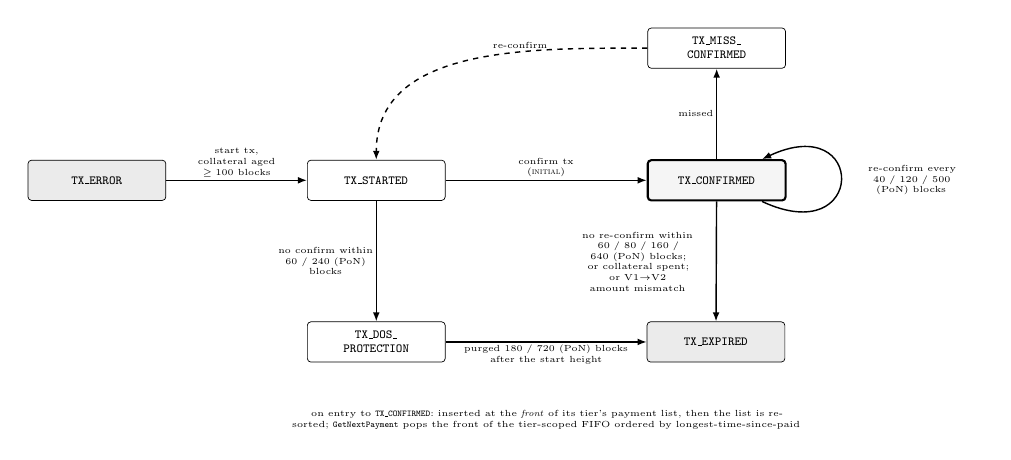
\begin{tikzpicture}[
  font=\scriptsize,
  st/.style={draw, rounded corners=2pt, align=center, minimum height=8mm, text width=26mm,
             inner xsep=2pt},
  term/.style={st, fill=black!8},
  live/.style={st, very thick, fill=black!4},
  arr/.style={-{Latex[length=1.8mm]}, thick},
  lbl/.style={font=\tiny, align=center, inner sep=1.5pt},
]
  \node[st]                                (start) {\texttt{TX\_STARTED}};
  \node[st,   below=24mm of start]         (dos)   {\texttt{TX\_DOS\_}\\\texttt{PROTECTION}};
  \node[live, right=40mm of start]         (conf)  {\texttt{TX\_CONFIRMED}};
  \node[term, right=40mm of dos]           (exp)   {\texttt{TX\_EXPIRED}};
  \node[st,   above=18mm of conf]          (miss)  {\texttt{TX\_MISS\_}\\\texttt{CONFIRMED}};
  \node[term, left=28mm of start]          (err)   {\texttt{TX\_ERROR}};

  \draw[arr] (err) -- node[lbl, above] {start tx,\\collateral aged\\$\ge 100$ blocks} (start);
  \draw[arr] (start) -- node[lbl, left, pos=0.5] {no confirm within\\60 / 240 (\PoN)\\blocks} (dos);
  \draw[arr] (start) -- node[lbl, above] {confirm tx\\(\textsc{initial})} (conf);
  \draw[arr] (dos) -- node[lbl, below] {purged 180 / 720 (\PoN) blocks\\after the start height} (exp);

  %% Self-loop kept on the right of TX_CONFIRMED so it clears TX_MISS_CONFIRMED above.
  \draw[arr] (conf) to[out=-25, in=25, looseness=7]
      node[lbl, right, pos=0.5, text width=27mm] {re-confirm every\\40 / 120 / 500 (\PoN) blocks} (conf);
  %% Both vertical edge labels sit on the left so nothing collides with the loop.
  \draw[arr] (conf) -- node[lbl, left, pos=0.5, text width=30mm]
      {no re-confirm within\\60 / 80 / 160 / 640 (\PoN) blocks;\\or collateral spent;\\or V1$\to$V2 amount mismatch} (exp);
  \draw[arr] (conf) -- node[lbl, left, pos=0.5] {missed} (miss);
  \draw[arr, dashed] (miss) to[out=180, in=90] node[lbl, above, pos=0.35] {re-confirm} (start);

  %% Spans the full width below both bottom states rather than sitting under TX_CONFIRMED,
  %% where it used to print on top of the conf-to-exp edge label.
  \node[lbl, below=13mm of $(dos)!0.5!(exp)$, text width=112mm]
    {on entry to \texttt{TX\_CONFIRMED}: inserted at the \emph{front} of its tier's payment list, then the
     list is re-sorted; \texttt{GetNextPayment} pops the front of the tier-scoped FIFO ordered by
     longest-time-since-paid};
  \end{tikzpicture}
\caption{The \FluxNode lifecycle state machine: states, transitions, and their governing height
constants \shipped \srccode{fluxd/\allowbreak{}src/\allowbreak{}fluxnode/\allowbreak{}fluxnode.h}{109--116}. Where two or more values are
shown, they are the successive versions of the constant selected by the active network upgrade, the
last being the \PoN-era value \srccode{fluxd/\allowbreak{}src/\allowbreak{}fluxnode/\allowbreak{}fluxnode.h}{23--44}. Only
\texttt{TX\_CONFIRMED} is in the paid set.}
\label{fig:fluxnode-lifecycle}
\end{figure}

\subsection{Tiers and collateral}
\label{sec:consensus-tiers}

\begin{table}[H]
\centering
\caption{\FluxNode collateral by tier and version, mainnet. Confirmation requirement is uniform across
tiers and versions.}
\label{tab:tiers}
\begin{tabular}{lrrll}
\toprule
Tier & V1 collateral & V2 collateral & Transition window $[\hgt_{\mathrm{start}},\hgt_{\mathrm{end}})$ & Confirmation \\
\midrule
Cumulus ($\tC$) & $\coll{\tC}=10{,}000\flux$ & $1{,}000\flux$ & $[1{,}076{,}532,\ 1{,}086{,}612)$ & 100 blocks \\
Nimbus ($\tN$)  & $\coll{\tN}=25{,}000\flux$ & $12{,}500\flux$ & $[1{,}081{,}572,\ 1{,}092{,}372)$ & 100 blocks \\
Stratus ($\tS$) & $\coll{\tS}=100{,}000\flux$ & $40{,}000\flux$ & $[1{,}087{,}332,\ 1{,}097{,}412)$ & 100 blocks \\
\bottomrule
\end{tabular}
\end{table}
\shipped \srccode{fluxd/\allowbreak{}src/\allowbreak{}fluxnode/\allowbreak{}fluxnode.h}{57--63} (V1/V2 amounts),
\srccode{fluxd/\allowbreak{}src/\allowbreak{}chainparams.cpp}{308--315} (transition windows),
\srccode{fluxd/\allowbreak{}src/\allowbreak{}fluxnode/\allowbreak{}fluxnode.h}{20} (100-block confirmation requirement,
\texttt{FLUXNODE\_MIN\_CONFIRMATION\_DETERMINISTIC}). Within a transition window, both the old and new
collateral amounts for that tier are accepted \shipped \srccode{fluxd/\allowbreak{}src/\allowbreak{}coins.cpp}{774--809}. The V2
amounts match the collateral recorded for every one of the 6{,}489 currently registered \FluxNodes in
the public registry \srcmeasured{api.runonflux.io/\allowbreak{}daemon/\allowbreak{}getzelnodecount}{2026-09-03}, i.e.\ the
migration is complete on mainnet as measured.

\subsection{Benchmarking and eligibility}
\label{sec:consensus-benchmark}

Confirming or re-confirming a \FluxNode requires a benchmark-signed transaction produced by
\fluxbench, a companion daemon that runs on the same host as \fluxd. \fluxbench measures CPU
throughput with \texttt{sysbench cpu -\allowbreak{}-\allowbreak{}cpu-\allowbreak{}max-\allowbreak{}prime=60000}
\shipped \srccode{fluxbench/\allowbreak{}src/\allowbreak{}fluxnode/\allowbreak{}benchmarks.cpp}{2066--2364}; disk write speed with three
\texttt{dd} runs per target, dropping the worst and averaging the remaining two, floored at
40 MB/s for reporting \shipped \srccode{fluxbench/\allowbreak{}src/\allowbreak{}fluxnode/\allowbreak{}benchmarks.h}{602--615,1020--1104},
\srccode{fluxbench/\allowbreak{}src/\allowbreak{}fluxnode/\allowbreak{}benchmarks.cpp}{1936}; bandwidth with the Ookla \texttt{speedtest} CLI,
combined with an \texttt{iftop} sample of bandwidth already in use
\shipped \srccode{fluxbench/\allowbreak{}src/\allowbreak{}fluxnode/\allowbreak{}benchmarks.cpp}{1358--1465,1980--2032}; and RAM headroom with
a \texttt{stress-ng} allocation test sized 8G/4G/2G for Stratus/Nimbus/Cumulus
\shipped \srccode{fluxbench/\allowbreak{}src/\allowbreak{}fluxnode/\allowbreak{}benchmarks.cpp}{3649--3667}.

\begin{table}[H]
\centering
\caption{Per-tier hardware thresholds enforced by \texttt{Validate\allowbreak{}Benchmark\allowbreak{}Requirements}, mainnet.}
\label{tab:benchmark-thresholds}
\begin{tabular}{lrrrrrrr}
\toprule
Tier & Cores & Threads & RAM & Storage & EPS & Disk write & Up/Down \\
\midrule
Cumulus & 2 & 4 & 7 GB & 220 GB & 240 & 180 MB/s & 25/25 Mbit/s \\
Nimbus  & 4 & 8 & 30 GB & 440 GB & 640 & 180 MB/s & 50/50 Mbit/s \\
Stratus & 8 & 16 & 61 GB & 880 GB & 1{,}520 & 400 MB/s & 100/100 Mbit/s \\
\bottomrule
\end{tabular}
\end{table}
\shipped \srccode{fluxbench/\allowbreak{}src/\allowbreak{}fluxnode/\allowbreak{}benchmarks.h}{58--84}. Cumulus's RAM requirement is 7 GB on
standard hardware and 3 GB on Jetson boards specifically
\shipped \srccode{fluxbench/\allowbreak{}src/\allowbreak{}fluxnode/\allowbreak{}benchmarks.h}{58--66}; measured bandwidth additionally
receives an additive tolerance bonus before the threshold check of $+2$/$+4$/$+9$ Mbit/s for
Cumulus/Nimbus/Stratus \shipped \srccode{fluxbench/\allowbreak{}src/\allowbreak{}fluxnode/\allowbreak{}benchmarks.h}{86--88}.

The result is signed by \texttt{BenchmarkSign}, which hashes the transaction's \texttt{sig},
\texttt{benchmarkTier}, \texttt{benchmark\allowbreak{}Sig\allowbreak{}Time}, and \texttt{ip} fields and signs with the fluxnode
key selected for the current time window
\shipped \srccode{fluxbench/\allowbreak{}src/\allowbreak{}fluxnode/\allowbreak{}benchmarks.cpp}{3439--3480}. The same verification routine,
\texttt{Check\allowbreak{}Benchmark\allowbreak{}Signature}, is linked into \fluxd and run as part of consensus validation of the
registration transaction \shipped \srccode{fluxbench/\allowbreak{}src/\allowbreak{}fluxnode/\allowbreak{}benchmarks.cpp}{3511--3522}. Three
further mechanisms can substitute a stored or historical value for a fresh measurement under specified
conditions — an enterprise-app short-circuit, a FluxOS-reported fallback, and a
single-thread-extrapolation fallback for the CPU test — and all three converge on the same
\texttt{Validate\allowbreak{}Benchmark\allowbreak{}Requirements()} acceptance gate
\shipped \srccode{fluxbench/\allowbreak{}src/\allowbreak{}fluxnode/\allowbreak{}benchmarks.cpp}{2178--2234,771--783,2883--3222}.

\paragraph{The property that does not hold.} On the \fluxd side, this same signature is verified
against \texttt{vec\allowbreak{}Benchmarking\allowbreak{}Public\allowbreak{}Keys} — five keys, each with a UNIX-timestamp validity window,
i.e.\ a rotating allowlist \shipped \srccode{fluxd/\allowbreak{}src/\allowbreak{}chainparams.cpp}{233--240}. These keys are
shared across the entire fleet: they identify "signed by something holding one of the five
network-wide benchmarking keys," not "signed by this specific operator's own key." \fluxd obtains the
benchmark result itself by shelling out — \texttt{popen()}-ing the local \texttt{fluxbench-cli}
process — and treats a returned \texttt{status:\allowbreak{}"complete"} field as sufficient to sign and broadcast
the registration transaction \shipped \srccode{fluxd/\allowbreak{}src/\allowbreak{}fluxnode/\allowbreak{}benchmarks.cpp}{74--102,227--291}.
The registration transaction must still match a valid on-chain collateral amount for the claimed tier
\shipped \srccode{fluxd/\allowbreak{}src/\allowbreak{}coins.cpp}{630--686}.

Put precisely: collateral binds the tier; the benchmark signature does not bind the hardware to the
tier it claims. An operator cannot register a tier they have not collateralized, but nothing beyond a
local, same-host process attests that the collateralized hardware in fact clears that tier's CPU/RAM
/disk/bandwidth thresholds in Table~\ref{tab:benchmark-thresholds}. \textbf{The correct claim is
benchmark-gating bypass, not tier forgery.} \S14 takes up the structurally identical problem one layer
up, for \ArcaneOS/\SAS attestation, and presents the planned bonded attestation network — where a bond
is put at stake rather than a shared secret being checked — as the mechanism intended to fix exactly
this property \planned \srcroadmap{timeline: new benchmark tool, signed node attestation}.

\subsection{The emergency-block path}
\label{sec:consensus-emergency}

A second, parallel block-authorization path exists outside \PoN sortition entirely, intended for
chain-halt recovery. A block whose \texttt{nodes\allowbreak{}Collateral} outpoint hash equals a fixed marker value
and whose index is 0 is treated as an \emph{emergency block}
\shipped \srccode{fluxd/\allowbreak{}src/\allowbreak{}emergencyblock.cpp}{24--30}. Such a block requires at least
\texttt{n\allowbreak{}Emergency\allowbreak{}Min\allowbreak{}Signatures} $= 2$ valid ECDSA signatures over \texttt{block.\allowbreak{}Get\allowbreak{}Hash()}, drawn from
a fixed set of 4 hardcoded public keys — a 2-of-4 multisignature, on mainnet and testnet alike
\shipped \srccode{fluxd/\allowbreak{}src/\allowbreak{}chainparams.cpp}{242--253}. Accepting an emergency block bypasses
\texttt{Check\allowbreak{}Proof\allowbreak{}Of\allowbreak{}Node} entirely \shipped \srccode{fluxd/\allowbreak{}src/\allowbreak{}pon/\allowbreak{}pon.cpp}{205--207} and bypasses the
per-node signature verification that an ordinary \PoN block requires
\shipped \srccode{fluxd/\allowbreak{}src/\allowbreak{}pon/\allowbreak{}pon.cpp}{236--252}.

The only gate on \emph{when} an emergency block may be produced is
\texttt{Is\allowbreak{}Emergency\allowbreak{}Block\allowbreak{}Allowed(n\allowbreak{}Height, n\allowbreak{}Time)}, which checks nothing beyond
\texttt{Is\allowbreak{}PONActive(n\allowbreak{}Height)} — there is no time-since-last-block check and no stall-detection logic
\shipped \srccode{fluxd/\allowbreak{}src/\allowbreak{}emergencyblock.cpp}{183--191} — despite a doc-comment on the type stating
"Can add additional restrictions like time delays"
\shipped \srccode{fluxd/\allowbreak{}src/\allowbreak{}emergencyblock.h}{41--44}. Concretely: any two holders of the four
emergency keys can mint a fully valid block at any height once \PoN is active, at any time, with no
on-chain evidence that the network was in fact stalled. This is a consensus-level centralization
surface, and it is stated here as one, not as a caveat.

The team intends to raise this threshold to \textbf{3-of-4 with a newly generated key set},
aligning consensus emergency-key governance with the bridge's 3-of-4 quorum (\S22), with no
activation height scheduled \planned \srcintent{design intake}. This is a stated direction of travel, not a deployed change: \texttt{n\allowbreak{}Emergency\allowbreak{}Min\allowbreak{}Signatures}
remains \textbf{2} against the current four-key set on mainnet and testnet today, which is why this
section states 2-of-4 \shipped \srccode{fluxd/\allowbreak{}src/\allowbreak{}chainparams.cpp}{242--253} above. Raising the
threshold does not change the shape of the disclosure just made: a 3-of-4 key set, like the 2-of-4
set it would replace, produces blocks outside \PoN{} eligibility and outside the per-node signature
check, with no time or stall-detection gating either before or after the change; what moves is only
the number of colluding or compromised keys required, from two of four to three of four. The absence
of any temporal or liveness constraint on \emph{when} an emergency block may be produced --- the more
consequential fact of the two --- is untouched by this parameter.

\subsection{What activation actually cost}
\label{sec:consensus-cost}

Activating \PoN required two emergency interventions visible directly in the code.
\texttt{MAX\_REORG\_LENGTH}, normally capped at 40 blocks
\shipped \srccode{fluxd/\allowbreak{}src/\allowbreak{}main.h}{74}, was overridden to 5{,}000 for heights
$[2{,}020{,}000,\ 2{,}025{,}000]$, commented "Temporary deep reorg limit during PON stabilization
period" \shipped \srccode{fluxd/\allowbreak{}src/\allowbreak{}main.cpp}{8983--8988}. A checkpoint cluster at heights
2{,}020{,}500; 2{,}021{,}000; 2{,}021{,}500; 2{,}022{,}000; and 2{,}029{,}000 was added, labelled "PON
activation and stabilization checkpoints - EMERGENCY FORK RECOVERY"
\shipped \srccode{fluxd/\allowbreak{}src/\allowbreak{}chainparams.cpp}{277--283}. \S\ref{sec:migration} returns to this as evidence for what a
consensus-level change actually requires of this network.

\subsection{Measured rotation}
\label{sec:consensus-rotation}

Under the front-of-list, longest-time-since-paid ordering described in
\S\ref{sec:consensus-lifecycle}, and given that each block pays one node from every tier, the expected
number of blocks between successive payments to a node in tier $x$ is $\rot{x} \defeq \ncount{x}$, the
tier's live node count. Table~\ref{tab:pon-rotation} compares this expectation against the maximum
observed gap in the public registry, chain tip height 2{,}917{,}115
\srcmeasured{api.runonflux.io/\allowbreak{}daemon/\allowbreak{}listzelnodes}{2026-09-03}.

\begin{table}[H]
\centering
\caption{Measured \PoN payment rotation vs. the deterministic per-tier model.}
\label{tab:pon-rotation}
\begin{tabular}{lrrrr}
\toprule
Tier & Nodes ($\ncount{\cdot}$) & Expected rotation ($\rot{\cdot}$, blocks) & Max blocks since paid & Duration at $\spacingpon$ \\
\midrule
Cumulus & 3{,}247 & 3{,}247 & 3{,}202 & 27.06 h \\
Nimbus  & 1{,}615 & 1{,}615 & 1{,}597 & 13.46 h \\
Stratus & 1{,}627 & 1{,}627 & 1{,}631 & 13.56 h \\
\bottomrule
\end{tabular}
\end{table}
\srcmeasured{api.runonflux.io/\allowbreak{}daemon/\allowbreak{}listzelnodes}{2026-09-03}. Stratus's observed maximum exceeds its
own node count by 4 blocks; this is consistent with the stale-entry skip loop in
\texttt{GetNextPayment} (\S\ref{sec:consensus-lifecycle}) rather than a violation of the FIFO ordering
rule. This measured rotation is the empirical confirmation on which \S7's fairness proposition for
\PNR depends: that proposition rests on the determinism of the \PoN \emph{payment} rotation, not on
placement determinism, and the two must not be conflated.

%% Drain this section's float queue before the next begins.
\FloatBarrier

\section{Monetary policy as deployed}
\label{sec:monetary-policy}

\Flux issues its native asset on a schedule fixed once, in \fluxd's consensus code, and not
adjusted by discretion afterward. Two different mechanisms have produced that schedule over the
chain's life: a Bitcoin-style halving curve during the proof-of-work era, and, since block height
$2{,}020{,}000$, a fixed initial block reward that decays by a constant fraction once a year under
Proof of Node. Neither curve reaches zero on any realistic horizon, and at least one of them was
adjusted by hand along the way rather than left to run the formula a reader might expect. This
section states the exact, currently-enforced arithmetic for both eras in the notation of
notation.tex, cross-checks the resulting figures against the network's own public reconciliation
of issued supply, and states plainly what the schedule implies for the long run: issuance never
stops, and only its rate settles to a small constant. Every subsequent economic claim in this
paper is denominated against the numbers derived here.

All amounts below are computed as integers over satoshi, $\mathrm{COIN} = 100{,}000{,}000\sat$ per
$\flux$ \shipped \srccode{fluxd/\allowbreak{}src/\allowbreak{}amount.h}{17}, matching \fluxd's \texttt{CAmount}
(\texttt{int64}) representation. ``$\lfloor\cdot\rfloor$'' denotes truncating (floor) integer
division throughout, exactly as C++ integer division behaves for non-negative operands
\srcdoc{flux-roadmap/supply/emission\_model.py:196-200, citing fluxd}. This distinction is
not cosmetic: the PoN reduction below is an $r$-fold sequence of \emph{independent} truncations,
not a single closed-form power, and the two are not interchangeable.

\subsection{The subsidy function}

\begin{definition}[Legacy proof-of-work subsidy]
\label{def:pow-subsidy}
For $0 \le \hgt < \hpon$,
$$
\subsidypow(\hgt) \;\defeq\;
\begin{cases}
0 & \hgt = 0 \\[4pt]
\premine = 13{,}020{,}000\flux & \hgt = 1 \\[4pt]
\floorfrac{150\,\mathrm{COIN}}{5000}\cdot \hgt & 2 \le \hgt < 2500 \\[6pt]
\floorfrac{150\,\mathrm{COIN}}{5000}\cdot (\hgt+1) & 2500 \le \hgt < 5000 \\[6pt]
\left\lfloor \dfrac{150\,\mathrm{COIN}}{2^{\,\min\left(\floorfrac{\hgt-2500}{655{,}350},\,2\right)}} \right\rfloor & 5000 \le \hgt < \hpon
\end{cases}
$$
\end{definition}
\shipped \srccode{fluxd/\allowbreak{}src/\allowbreak{}main.cpp}{2818-2852}, constants \srccode{fluxd/\allowbreak{}src/\allowbreak{}chainparams.cpp}{90-91}.
This is the literal transcription of \texttt{Get\allowbreak{}Block\allowbreak{}Subsidy}'s legacy branch as currently compiled
\shipped \srccode{flux-roadmap/\allowbreak{}supply/\allowbreak{}emission\_model.py}{207-218}. The chain's actual historical
payout for heights $1$--$4{,}999$ differs from this formula by one block index (an older binary
paid the premine at height $2$, not $1$, and shifted the slow-start ramp accordingly)
\shipped \srccode{flux-roadmap/\allowbreak{}supply/\allowbreak{}emission\_model.py}{220-229}; that discrepancy is the source
of the persistent offset discussed in \S\ref{sec:mp-discrepancy} below. The code's separate
$\text{halvings}\ge 64 \Rightarrow 0$ branch is never reached before $\hpon$ and so never fires on
the deployed chain \shipped \srccode{fluxd/\allowbreak{}src/\allowbreak{}main.cpp}{2839-2840}.

\begin{definition}[Proof-of-Node subsidy]
\label{def:pon-subsidy}
For $\hgt \ge \hpon$, let
\begin{gather*}
r(\hgt) \;\defeq\; \min\!\left(\floorfrac{\hgt-\hpon}{\redint},\ \redmax\right),
\qquad
s_0 \defeq 14\cdot\mathrm{COIN} = 1{,}400{,}000{,}000\sat, \\
s_{k+1} \defeq \left\lfloor s_k \cdot \redfac \right\rfloor,\ \ \redfac = \frac{9}{10},
\end{gather*}
for $k = 0,\dots,\redmax-1$. Then
$$
\subsidypon(\hgt) \;\defeq\; s_{r(\hgt)}.
$$
\end{definition}
\shipped \srccode{fluxd/\allowbreak{}src/\allowbreak{}main.cpp}{2799-2816}; $\hpon = 2{,}020{,}000$
\shipped \srccode{fluxd/\allowbreak{}src/\allowbreak{}chainparams.cpp}{153}; $\redint = 1{,}051{,}200$ blocks
($365\times24\times60\times2$, one year at the 30-second PoN spacing)
\shipped \srccode{fluxd/\allowbreak{}src/\allowbreak{}chainparams.cpp}{157}; $\redmax = 20$
\shipped \srccode{fluxd/\allowbreak{}src/\allowbreak{}chainparams.cpp}{158}. The combined block subsidy is
$\subsidy(\hgt) = \subsidypow(\hgt)$ for $\hgt < \hpon$ and $\subsidypon(\hgt)$ otherwise
\shipped \srccode{fluxd/\allowbreak{}src/\allowbreak{}main.cpp}{2796-2798}.

\textbf{Integer semantics.} $s_{r}$ is $r$ \emph{independently truncated} multiplications, not a
closed form: $s_r \neq \left\lfloor s_0 \cdot (9/10)^{r} \right\rfloor$ in general, because each
step's rounding error compounds on top of the previous step's rather than being computed once
against the original $s_0$ \shipped \srccode{fluxd/\allowbreak{}src/\allowbreak{}main.cpp}{2811-2813}. At $r=20$ the two
expressions already differ at the eight printed decimal places used below: the iterated value is
$1.70207313\flux$ against $1.70207316\flux$ for the closed form, and the two first diverge at $r=10$
\shipped \srccode{flux-roadmap/\allowbreak{}supply/\allowbreak{}emission\_model.py}{195-204}; the paper
states the iterated definition as the one \fluxd actually computes.

\subsection{The frozen halving}
\label{sec:mp-frozen-halving}

The $\min(\cdot,2)$ term in Definition~\ref{def:pow-subsidy} is not an idealization; it is a
hand-frozen consensus rule. \texttt{Get\allowbreak{}Block\allowbreak{}Subsidy}'s legacy branch reads
\texttt{if (halvings >= 2) \{ nSubsidy >>= 2; return nSubsidy; \}}, with an in-source comment
describing it as a ``temp solution while we work on the next blockchain improvement protocols''
\shipped \srccode{fluxd/\allowbreak{}src/\allowbreak{}main.cpp}{2842-2848}. Emission was therefore held at the second-halving
level, $37.5\flux$/block, rather than continuing to halve every $655{,}350$ blocks
\shipped \srccode{fluxd/\allowbreak{}src/\allowbreak{}chainparams.cpp}{91}. This was not merely a theoretical stopping point:
had halving continued, a third halving (to $18.75\flux$/block) would have taken effect at height
$1{,}968{,}550 = 2500 + 3\times655{,}350$, which is before $\hpon = 2{,}020{,}000$; instead, the
frozen floor held the reward at $37.5\flux$/block for the roughly $51{,}450$ blocks between that
point and PoN activation, at which point the entire legacy path was replaced by
Definition~\ref{def:pon-subsidy} \shipped \srccode{fluxd/\allowbreak{}src/\allowbreak{}main.cpp}{2845-2848}.

\subsection{Tier partition and the dev-fund remainder}
\label{sec:mp-tier-devfund}

\begin{definition}[PoN tier reward]
For tier $X \in \tiers = \{\tC,\tN,\tS\}$ and $\hgt \ge \hpon$,
$$
\mathrm{reward}_X(\hgt) \;\defeq\; \left\lfloor \subsidypon(\hgt) \cdot \frac{\tbase{X}}{14\flux} \right\rfloor,
$$
with $\tbase{\tC} = 1.0\flux$, $\tbase{\tN} = 3.5\flux$, $\tbase{\tS} = 9.0\flux$ --- ratios chosen
so that two Nimbus earn less than one Stratus while three earn more, and three Cumulus less than one
Nimbus while four earn more \citep{fluxrewardmodel} ---
\shipped \srccode{fluxd/\allowbreak{}src/\allowbreak{}main.cpp}{2892-2895}, applied against the current, possibly-reduced
$\subsidypon(\hgt)$, not against a value fixed at PoN activation
\shipped \srccode{fluxd/\allowbreak{}src/\allowbreak{}main.cpp}{2886-2939}.
\end{definition}

The $14\flux$ denominator is coded as \texttt{PON\_INITIAL\_TOTAL}, a separate local constant in
\texttt{Get\allowbreak{}Fluxnode\allowbreak{}Subsidy}, rather than read from the consensus parameter
\texttt{n\allowbreak{}PONInitial\allowbreak{}Subsidy} that fixes $s_0$ in Definition~\ref{def:pon-subsidy}
\shipped \srccode{fluxd/\allowbreak{}src/\allowbreak{}main.cpp}{2892}. A future upgrade that changed
\texttt{n\allowbreak{}PONInitial\allowbreak{}Subsidy} without also editing this literal would silently desynchronize the
tier ratios from the actual base subsidy; this is a maintenance hazard in the deployed code, stated
here because it bears on what a future constant change could do without touching the tier logic at
all \shipped \srccode{fluxd/\allowbreak{}src/\allowbreak{}main.cpp}{2892}.

\begin{definition}[Dev-fund remainder]
$$
\devfund(\hgt) \;\defeq\; \subsidypon(\hgt) - \mathrm{reward}_{\tC}(\hgt) - \mathrm{reward}_{\tN}(\hgt) - \mathrm{reward}_{\tS}(\hgt), \qquad \hgt \ge \hpon.
$$
\end{definition}
\shipped \srccode{fluxd/\allowbreak{}src/\allowbreak{}main.cpp}{2877-2884} (\texttt{Get\allowbreak{}Min\allowbreak{}Dev\allowbreak{}Fund\allowbreak{}Amount}). At $r=0$, the
unreduced $14\flux$ subsidy, $\devfund = 0.5\flux = 50{,}000{,}000\sat$, i.e.\ $1/28 \approx 3.57\%$
of PoN emission. Because $\devfund$ is defined as a remainder of the \emph{current} subsidy rather
than a fixed floor, this share decays proportionally as $\subsidypon$ reduces
\shipped \srccode{flux-roadmap/\allowbreak{}supply/\allowbreak{}emission\_model.py}{358-368}.

Payment is consensus-enforced twice, independently. Loosely: any post-PoN coinbase lacking an
output of at least $\devfund(\hgt)$ to the hardcoded address is rejected with
\texttt{"tx-\allowbreak{}coinbase-\allowbreak{}missing-\allowbreak{}dev-\allowbreak{}funding"} \shipped \srccode{fluxd/\allowbreak{}src/\allowbreak{}main.cpp}{1231-1249}.
Strictly: \texttt{Fluxnode\allowbreak{}Cache::\allowbreak{}Check\allowbreak{}Fluxnode\allowbreak{}Payout} independently requires the coinbase value not
already claimed by a tier payout to be at least $\devfund(\hgt)$
\shipped \srccode{fluxd/\allowbreak{}src/\allowbreak{}fluxnode/\allowbreak{}fluxnode.cpp}{837-875}. The mainnet address is
\texttt{t3h\allowbreak{}Pu1YDe\allowbreak{}GUCp8m7BQCnn\allowbreak{}NUm\allowbreak{}RMJBa5Rady\allowbreak{}A} \shipped \srccode{fluxd/\allowbreak{}src/\allowbreak{}chainparams.cpp}{306}.

No source comment names this remainder a ``dev fund'' at the point where the tier ratios
themselves are defined; the routing is discoverable only by following
\texttt{Get\allowbreak{}Min\allowbreak{}Dev\allowbreak{}Fund\allowbreak{}Amount}'s call graph out to the two enforcement sites above, not from any
single comment at the site of the constants \shipped \srccode{fluxd/\allowbreak{}src/\allowbreak{}main.cpp}{2877-2884}. That
is a documentation gap worth stating plainly rather than leaving for a reader to reconstruct.

\subsection{One-off and recurring fund payouts}
\label{sec:mp-fund-payouts}

Three further payments are enforced directly in coinbase validation, by exact scriptPubKey and
amount match, independent of the tier/dev-fund split above
\shipped \srccode{fluxd/\allowbreak{}src/\allowbreak{}main.cpp}{1252-1304}: two one-off payments and one recurring schedule.

\begin{table}[H]
\centering
\caption{One-off and recurring consensus-enforced fund payouts, mainnet. All entries \shipped,
cited directly to \fluxd.}
\label{tab:fund-payouts}
\begin{tabular}{@{}lllll@{}}
\toprule
Payment & Address & Height / schedule & Amount & Provenance \\
\midrule
Exchange fund & \texttt{t3PMbb\allowbreak{}A5YBMrj\allowbreak{}SD3d\allowbreak{}D16SSd\allowbreak{}XKu\allowbreak{}Kovwmj6t\allowbreak{}S} & $\hgt = 836{,}274$, one-off &
$7{,}500{,}000\flux$ & \srccode{fluxd/\allowbreak{}src/\allowbreak{}chainparams.cpp}{293-294} \\
Foundation fund & \texttt{t3Xj\allowbreak{}YMBvwxn\allowbreak{}XVv9jqg4Cgok\allowbreak{}Z3f7k\allowbreak{}Ao\allowbreak{}XPQL8} & $\hgt = 836{,}994$, one-off &
$2{,}500{,}000\flux$ & \srccode{fluxd/\allowbreak{}src/\allowbreak{}chainparams.cpp}{297-298} \\
Swap pool & \texttt{t3Thb\allowbreak{}Wog\allowbreak{}Do\allowbreak{}Aj\allowbreak{}Gu\allowbreak{}S6DEnm\allowbreak{}N1GWJBRb\allowbreak{}Vj\allowbreak{}SUK4T} & from $\hgt = 837{,}714$, every
$21{,}600$ blocks, $\times 10$ & $22{,}000{,}000\flux$ per tranche ($220{,}000{,}000\flux$ total) &
\srccode{fluxd/\allowbreak{}src/\allowbreak{}chainparams.cpp}{301-304} \\
\bottomrule
\end{tabular}
\end{table}

\subsection{The supply function}
\label{sec:mp-supply}

\begin{definition}[Cumulative supply]
\label{def:supply}
\begin{multline*}
\supply(\hgt) \;=\; \mathrm{premine}(\hgt) + \mathrm{pow\_slow\_start}(\hgt)
  + \mathrm{pow}_{150}(\hgt) + \mathrm{pow}_{75}(\hgt) + \mathrm{pow}_{37.5}(\hgt) \\
  {}+ \mathrm{exch}(\hgt) + \mathrm{found}(\hgt) + \mathrm{swap}(\hgt) + \mathrm{pon}(\hgt),
\end{multline*}
with
\begin{align*}
\mathrm{premine}(\hgt) &= \premine \cdot \indic{\hgt \ge 2} \\
\mathrm{pow\_slow\_start}(\hgt) &= \textstyle\sum_{k=2}^{\min(\hgt,\,4999)} \subsidypow(k) \\
\mathrm{pow}_{150}(\hgt) &= 150\flux \cdot \big|\{k : 5000 \le k \le \min(\hgt,657{,}849)\}\big| \\
\mathrm{pow}_{75}(\hgt) &= 75\flux \cdot \big|\{k : 657{,}850 \le k \le \min(\hgt,1{,}313{,}199)\}\big| \\
\mathrm{pow}_{37.5}(\hgt) &= 37.5\flux \cdot \big|\{k : 1{,}313{,}200 \le k \le \min(\hgt,2{,}019{,}999)\}\big| \\
\mathrm{exch}(\hgt) &= 7{,}500{,}000\flux \cdot \indic{\hgt \ge 836{,}274} \\
\mathrm{found}(\hgt) &= 2{,}500{,}000\flux \cdot \indic{\hgt \ge 836{,}994} \\
\mathrm{swap}(\hgt) &= 22{,}000{,}000\flux \cdot \textstyle\sum_{i=0}^{9} \indic{\hgt \ge 837{,}714 + 21{,}600\,i} \\
\mathrm{pon}(\hgt) &= \textstyle\sum_{k=\hpon}^{\hgt} \subsidypon(k) \cdot \indic{\hgt \ge \hpon}
\end{align*}
\end{definition}
\shipped \srccode{flux-roadmap/\allowbreak{}supply/\allowbreak{}emission\_model.py}{321-367}. The premine trigger height
above uses $2$ (the observed mode used for every current- and historical-supply figure in this
section); the literal code branch triggers at height $1$ instead
\shipped \srccode{fluxd/\allowbreak{}src/\allowbreak{}main.cpp}{2820-2822} — the one-block difference re-enters as part of
the discrepancy in \S\ref{sec:mp-discrepancy}. All nine terms are additive; the PoW and PoN
subsidy terms are mutually exclusive by height, and the premine, exchange, foundation and
swap-pool terms are new issuance layered on top of whichever subsidy term is active
\shipped \srccode{flux-roadmap/\allowbreak{}supply/\allowbreak{}emission\_model.py}{469-477}. The tier rewards and dev-fund
remainder of \S\ref{sec:mp-tier-devfund} are a display-only split of $\mathrm{pon}(\hgt)$; they are
never added on top of it \shipped \srccode{flux-roadmap/\allowbreak{}supply/\allowbreak{}emission\_model.py}{358-368}.

\begin{proposition}[No terminal supply]
\label{prop:no-terminal-supply}
$\supply$ does not converge at any height. For every $\hgt \ge \hgt_{20} \defeq \hpon + \redmax\cdot\redint = 23{,}044{,}000$,
$$
\subsidypon(\hgt) = s_{20} = 170{,}207{,}313\sat = 1.70207313\flux
$$
is constant, because the reduction loop in Definition~\ref{def:pon-subsidy} terminates after
$\redmax = 20$ iterations rather than continuing indefinitely
\shipped \srccode{fluxd/\allowbreak{}src/\allowbreak{}main.cpp}{2811-2816}. Consequently $\supply$ grows without bound at the
fixed asymptotic rate
$$
s_{20} \cdot \redint = 1.70207313\flux \times 1{,}051{,}200 = 1{,}789{,}219.274256\ \flux/\mathrm{year}, \quad \text{forever}.
$$
\end{proposition}
\shipped \srccode{flux-roadmap/\allowbreak{}supply/\allowbreak{}emission\_model.py}{514-546}, executed 2026-09-03.
Height $\hgt_{20} = 23{,}044{,}000$ is a direct consequence of the consensus constants above and is
exact; the corresponding calendar date, $\sim$2045-10-20, is a 30-second-spacing extrapolation from
the PoN-activation timestamp anchor, and the model itself validates that extrapolation only against
block $2{,}816{,}820$, about $800{,}000$ blocks after activation, not over horizons this long
\srcdoc{flux-roadmap/supply/emission\_model.py:389-391}.
One PoN year later, at height $24{,}095{,}199$ ($\sim$2046-10-20, same caveat), cumulative supply is
$548{,}043{,}625.860464\flux$ \shipped \srccode{flux-roadmap/\allowbreak{}supply/\allowbreak{}emission\_model.py}{321-367}.
This is not a cap; it is only the point at which the annual emission \emph{rate} has become
constant, per Proposition~\ref{prop:no-terminal-supply}. The team's own public statement is
consistent with this derivation: ``block rewards reduce 10\% a year for twenty years and then
continue at a small fixed amount indefinitely — about 1.79 million FLUX a year, forever''
\srcroadmap{flux-roadmap-public.md:189}.

\textbf{Current supply.} $\supply(2{,}912{,}015) = 429{,}466{,}823.9700\flux$, observed mode,
computed 2026-09-03 \shipped \srccode{flux-roadmap/\allowbreak{}supply/\allowbreak{}emission\_model.py}{321-367}. This is
consistent with the team's own public reconciliation — ``about 428.1 million FLUX, at block
$\sim$2,816,845 \dots reconciles with our emission model to within 0.0005\%'' —
\srcroadmap{flux-roadmap-public.md:185}, an earlier height on the same monotone curve.

\textbf{\maxmoney is not a supply cap.} $\maxmoney = 440{,}000{,}000\flux$ is defined in
\texttt{MoneyRange()} as a per-transaction/output sanity bound, not a chain-wide accumulator
\shipped \srccode{fluxd/\allowbreak{}src/\allowbreak{}amount.h}{22-31}. Cumulative issuance crosses this value at height
$3{,}730{,}295$ ($\sim$2027-06-11) \shipped \srccode{flux-roadmap/\allowbreak{}supply/\allowbreak{}emission\_model.py}{550-561},
and nothing in consensus checks or breaks when it does. The team states this publicly in the same
terms: ``Neither 440 million nor 560 million is a cap enforced by the protocol \dots issuance
passes it in 2027 without anything breaking \dots there is no hard cap today. We would rather say
that than repeat a number'' \srcroadmap{flux-roadmap-public.md:189,191}.

\subsection{Plots}
\label{sec:mp-plots}

\begin{figure}[H]
\centering
\begin{tikzpicture}
\begin{axis}[
    width=\linewidth, height=6cm,
    xlabel={Year},
    ylabel={Cumulative supply $\supply(\hgt)$ [\flux]},
    xmin=2026, xmax=2060,
    grid=major,
]
\addplot[thick, blue, mark=none] table[x index=0, y index=2] {../data/emission.dat};
\draw[densely dashed] ({axis cs:2045.8,0}|-{rel axis cs:0,1}) -- ({axis cs:2045.8,0}|-{rel axis cs:0,0})
    node[pos=0.08, right, font=\scriptsize] {$\hgt=23{,}044{,}000$: 20th reduction};
\end{axis}
\end{tikzpicture}
\caption{Cumulative issued \Flux supply, 2026--2060, mode=observed
\shipped \srccode{flux-roadmap/\allowbreak{}supply/\allowbreak{}emission\_model.py}{321-367}. Data: \texttt{paper/\allowbreak{}data/\allowbreak{}emission.\allowbreak{}dat}
(columns \texttt{year}, \texttt{height}, \texttt{cumulative\_supply}, \texttt{annual\_emission},
\texttt{pow\_emission}, \texttt{pon\_emission}). The dashed line marks the onset of the flat
tail rate, per Proposition~\ref{prop:no-terminal-supply}, read from
\texttt{paper/\allowbreak{}data/\allowbreak{}pon\_reductions.\allowbreak{}dat} row $n=20$.}
\label{fig:cumulative-supply}
\end{figure}

\begin{figure}[H]
\centering
\begin{tikzpicture}
\begin{axis}[
    width=\linewidth, height=6cm,
    xlabel={Year},
    ylabel={Annual emission [\flux/\text{yr}]},
    xmin=2026, xmax=2060,
    grid=major,
]
\addplot[thick, red!70!black, mark=none] table[x index=0, y index=3] {../data/emission.dat};
\end{axis}
\end{tikzpicture}
\caption{Annual \Flux emission by calendar year. \texttt{pow\_emission} is exactly zero for every
plotted year (all postdate \PoN activation) \shipped \srccode{flux-roadmap/\allowbreak{}supply/\allowbreak{}emission\_model.py}{299-318}.
Data: \texttt{paper/\allowbreak{}data/\allowbreak{}emission.\allowbreak{}dat}, column \texttt{annual\_emission}. From calendar year 2046
onward the series is $1{,}789{,}219.274256\flux$ per 365-day year, per
Proposition~\ref{prop:no-terminal-supply}; leap years (2048, 2052, \ldots) carry one more day of
blocks and read $1{,}794{,}121.2449\flux$.}
\label{fig:annual-emission}
\end{figure}
%% verified 2026-09-04: emission.dat header is "# year height cumulative_supply annual_emission
%% pow_emission pon_emission"; the cumulative-supply plots read y index=2 and the annual-emission
%% plot y index=3, both matching their axis labels. pon_reductions.dat is not consumed by any
%% plot. (Build note; not paper text.)

\subsection{A discrepancy in the published model}
\label{sec:mp-discrepancy}

The emission model's own docstring claims that its two computation modes — \texttt{observed}
(what mainnet actually paid) and \texttt{code} (a literal transcription of the current
\texttt{Get\allowbreak{}Block\allowbreak{}Subsidy}) — differ by $0.06\flux$ in total, and calls the choice between them
``irrelevant at publication precision'' \srcdoc{flux-roadmap/supply/emission\_model.py:105-106}.
Executing the model shows an exact, height-independent difference of $150.00000000\flux$ at every
tested height $\ge 5{,}000$, arising from the one-block index shift itself, which lowers the payout of
every one of the $4{,}996$ ramp blocks by $0.03\flux$ and of blocks $2$ and $2{,}500$ by $0.06\flux$
each, where the docstring's figure counts block $2$ alone
\shipped \srccode{flux-roadmap/\allowbreak{}supply/\allowbreak{}emission\_model.py}{207-229}. This is a
finding about the published emission model's own arithmetic, not about \fluxd's consensus code,
which is unaffected. This paper uses \texttt{observed} mode throughout, as the model's own default
for historical and current-supply claims; full derivation and reproduction steps are in
Appendix~C.

\subsection{Baseline for what follows}

The subsidy, tier, dev-fund and fund-payout functions given here are the quantities Section~7
measures Progressive Node Reward parity against, and every issuance, supply or operator-income
figure elsewhere in this paper is denominated against the schedule fixed in this section.

%% Drain this section's float queue before the next begins.
\FloatBarrier

\section{Parallel assets: the current multi-chain footprint and the case for consolidation}
\label{sec:parallel-assets}

A holder of \Flux is not necessarily holding anything on the \Flux main chain. Since early in the
project's life, tokens representing \flux have also been issued on other blockchains — a
``parallel asset'' is a token on a chain other than \Flux's own that is meant to track a \flux
balance, historically backed by reserves held at addresses the team controls rather than by a
supply-capped, on-chain-verifiable contract \srcroadmap{flux-roadmap-public.md:96}. Each such asset
adds a chain whose contract, custody keys, exchange relationships and accounting have to be kept in
sync with the main chain and with each other. This section inventories what actually exists today,
shows that the inventory has grown rather than shrunk even as the team has stated an intent to
consolidate it, describes the mechanism by which a parallel asset changes hands today and the trust
it requires, and states the settled but only partially resolved plan for reducing the footprint.
The bridging construction itself — mint-and-burn with attested proof-of-reserve — is specified in
\S\ref{sec:bridging}; this section establishes why that construction is needed and what it has to
replace.

\subsection{The inventory}
\label{sec:pa-inventory}

Table~\ref{tab:parallel-assets} lists every chain on which a \flux-denominated token is identified
by contract or account address in the surveyed code, together with the exact on-chain identifier
and its source. Ten entries are shipped by this definition: the address or module name appears in
code that a live, currently-operated service uses to read balances, construct transfers, or both.

\begin{table}[H]
\centering
\footnotesize
\caption{The parallel-asset footprint as read from the team's own indexing and swap tooling.
Ethereum, BNB Chain, Polygon and Avalanche C-Chain addresses agree between \texttt{holder-\allowbreak{}snapshot}
and \texttt{flux-\allowbreak{}supply-\allowbreak{}tracker}; Base appears only in the latter. \shipped for every row —
each identifier is consumed by code that treats it as a live contract or account, not asserted from
a roadmap or design note. None of these addresses was independently verified against the chain
itself by the evidence gathering this section relies on.}
\label{tab:parallel-assets}
\begin{tabular}{@{}llp{6.1cm}l@{}}
\toprule
Asset & Chain & Contract / account identifier & Provenance \\
\midrule
FLUX (ERC-20) & Ethereum &
\texttt{\scriptsize 0x720cd16b\allowbreak{}011b987d\allowbreak{}a3518fbf\allowbreak{}38c3071d\allowbreak{}4f0d1495} &
\srccode{holder-snapshot/\allowbreak{}index.js}{22}\srccode{flux-supply-tracker/\allowbreak{}index.html}{310} \\
FLUX (BEP-20) & BNB Chain &
\texttt{\scriptsize 0xaff9084f\allowbreak{}23745858\allowbreak{}79e8b434\allowbreak{}c399e29e\allowbreak{}80cce635} &
\srccode{holder-snapshot/\allowbreak{}index.js}{23}\srccode{flux-supply-tracker/\allowbreak{}index.html}{319} \\
FLUX (ERC-20-compatible) & Polygon &
\texttt{\scriptsize 0x\allowbreak{}A2bb7A68\allowbreak{}c46b53f6\allowbreak{}Bb\allowbreak{}F6c\allowbreak{}C91\allowbreak{}C865Ae24\allowbreak{}7A82E99B} &
\srccode{holder-snapshot/\allowbreak{}index.js}{26}\srccode{flux-supply-tracker/\allowbreak{}index.html}{328} \\
FLUX (ERC-20-compatible) & Avalanche C-Chain &
\texttt{\scriptsize 0xc4B06F17\allowbreak{}ECc\allowbreak{}B2215\allowbreak{}a5DBf042\allowbreak{}C672101F\allowbreak{}c20da\allowbreak{}F55} &
\srccode{holder-snapshot/\allowbreak{}index.js}{24}\srccode{flux-supply-tracker/\allowbreak{}index.html}{337} \\
FLUX (ERC-20-compatible) & Base &
\texttt{\scriptsize 0xb008bdcf\allowbreak{}9cdff9da\allowbreak{}684a1909\allowbreak{}41dc3dca\allowbreak{}8c2cdd44} &
\srccode{flux-supply-tracker/\allowbreak{}index.html}{346} (absent from \texttt{holder-\allowbreak{}snapshot}) \\
FLUX (SPL mint) & Solana &
\texttt{\scriptsize FLUX1wa2\allowbreak{}Gmbt\allowbreak{}SB6Z\allowbreak{}Gi2p\allowbreak{}TNb\allowbreak{}V\allowbreak{}Cw3z\allowbreak{}Ee\allowbreak{}Kn\allowbreak{}a\allowbreak{}PCk\allowbreak{}Pt\allowbreak{}FX\allowbreak{}xq\allowbreak{}Xe} &
\srccode{holder-snapshot/\allowbreak{}index.js}{20}\srccode{flux-supply-tracker/\allowbreak{}index.html}{355} \\
FLUX (ASA) & Algorand &
\texttt{\scriptsize 1029804829} &
\srccode{holder-snapshot/\allowbreak{}index.js}{27}\srccode{flux-supply-tracker/\allowbreak{}index.html}{364} \\
FLUX (Ergo token) & Ergo &
\texttt{\scriptsize e8b20745\allowbreak{}ee9d1881\allowbreak{}7305f32e\allowbreak{}b2101583\allowbreak{}1a48f02d\allowbreak{}40980de6\allowbreak{}e849f886\allowbreak{}dca7f807} &
\srccode{holder-snapshot/\allowbreak{}index.js}{25}\srccode{flux-supply-tracker/\allowbreak{}index.html}{373} \\
FLUX (TRC-20) & Tron &
\texttt{\scriptsize TWr6yzuk\allowbreak{}Rw\allowbreak{}Z53HDe\allowbreak{}3bzc\allowbreak{}C8RC\allowbreak{}Tbi\allowbreak{}Ka4Zz\allowbreak{}b6} &
\srccode{holder-snapshot/\allowbreak{}index.js}{21}\srccode{flux-supply-tracker/\allowbreak{}index.html}{382} \\
FLUX (Pact fungible-v2) & Kadena &
\texttt{\scriptsize runonflux.\allowbreak{}flux} &
\srccode{flux-kda/\allowbreak{}flux.pact}{1-3}\srccode{flux-supply-tracker/\allowbreak{}index.html}{391} \\
\bottomrule
\end{tabular}
\end{table}

The EVM entries (Ethereum, BNB Chain, Polygon, Avalanche C-Chain, Base) are read via each chain's
ERC-20 \texttt{Transfer} log topic by the same crawler code
\shipped \srccode{holder-snapshot/\allowbreak{}eth.js}{63-88}, so they are one contract shape deployed five
times rather than five independent designs; the Ethereum/BNB-Chain pair is additionally attested by
its own source repository as the same compiled bytecode on both chains
\srcdoc{flux-eth-bsc/README.md:1-14}. That repository's own Truffle build record, however,
contains no deployed network address for any chain — the \texttt{networks} field of
\texttt{flux-eth-bsc/\allowbreak{}bin/\allowbreak{}Flux.\allowbreak{}json} is absent or empty \srcdoc{flux-eth-bsc/bin/Flux.json,
\texttt{networks} field}. Every address in Table~\ref{tab:parallel-assets} is taken
from the team's own indexing tools, not from the contract-source repository itself.

\subsection{The trend is the wrong way}
\label{sec:pa-trend}

Three snapshots of the team's own tooling, taken at different times, give three different chain
counts, and the count only goes up. \texttt{holder-\allowbreak{}snapshot}'s \texttt{README} documents support
for six chains \srcdoc{holder-snapshot/README.md:4-10}; its own \texttt{index.js} code
handles eight, adding Polygon and Algorand beyond what the README claims
\shipped \srccode{holder-snapshot/\allowbreak{}index.js}{20-27}; and \texttt{flux-\allowbreak{}supply-\allowbreak{}tracker}'s live
\texttt{CHAINS} configuration, last touched 2026-08-05, carries ten, adding Base and folding Kadena
in as a tenth \shipped \srccode{flux-supply-tracker/\allowbreak{}index.html}{308-397}. Read plainly: documentation
said six, shipped code already did eight, and the newest measurement tool does ten. This is the
team's own data, gathered to run its own reserve and rich-list computations, and it is the single
strongest argument in this section for consolidation — not because any one parallel asset is
individually a problem, but because the footprint has been growing under a team that has also, in
the same period, stated a public non-goal of not adding new parallel-asset chains while the existing
ones are consolidated \srcroadmap{flux-roadmap-public.md:209}. The growth already happened before
that statement was made, which is exactly why consolidation is a live problem and not a preventative
one.

\begin{figure}[H]
\centering
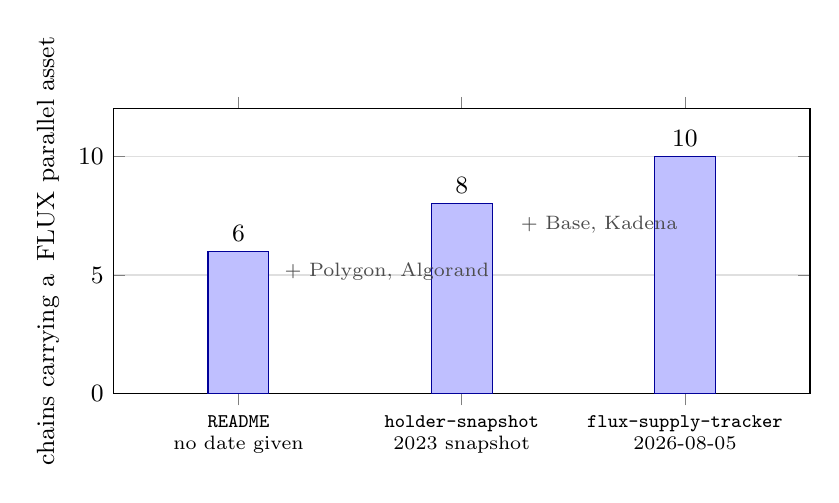
\begin{tikzpicture}[font=\small]
\begin{axis}[
  width=0.86\linewidth, height=5.2cm,
  ybar, bar width=22pt,
  ymin=0, ymax=12,
  ylabel={chains carrying a \flux{} parallel asset},
  symbolic x coords={README, snapshot, tracker},
  xtick=data,
  xticklabels={%
    {\texttt{README}\\{\scriptsize no date given}},
    {\texttt{holder-\allowbreak{}snapshot}\\{\scriptsize 2023 snapshot}},
    {\texttt{flux-\allowbreak{}supply-\allowbreak{}tracker}\\{\scriptsize 2026-08-05}}},
  xticklabel style={align=center, font=\scriptsize},
  nodes near coords, nodes near coords style={font=\small\bfseries},
  ymajorgrids, major grid style={gray!25},
  enlarge x limits=0.28,
]
\addplot[fill=blue!25, draw=blue!60!black] coordinates {(README,6) (snapshot,8) (tracker,10)};
\end{axis}
\node[anchor=west, font=\scriptsize, text=black!70] at (2.05,1.55) {$+$ Polygon, Algorand};
\node[anchor=west, font=\scriptsize, text=black!70] at (5.05,2.15) {$+$ Base, Kadena};
\end{tikzpicture}
\caption{The parallel-asset footprint grew between every source that documents it, and no single
source is current. The count is six in the repository README, eight in the \texttt{holder-\allowbreak{}snapshot}
code path, and ten in \texttt{flux-\allowbreak{}supply-\allowbreak{}tracker}; the two chains added at each step are annotated.
This is the measurement problem \S\ref{sec:pa-supply-accounting} addresses: a consolidation cannot be
scoped from a source that does not know how many chains exist. \shipped
\srcdoc{holder-snapshot/README.md:4-10}\srccode{holder-snapshot/\allowbreak{}index.js}{20--27}\srccode{flux-supply-tracker/\allowbreak{}index.html}{308--397}.}
\label{fig:pa-chain-growth}
\end{figure}

One further caveat belongs here rather than in a footnote: as of the most recent local state of
\texttt{holder-\allowbreak{}snapshot}, only its Ergo crawl is actually invoked — every other chain's
\texttt{start()} call is commented out \shipped \srccode{holder-snapshot/\allowbreak{}index.js}{29-36} — so the
tool that produced the ten-chain figure is not itself being run against ten chains today. That
does not change the ten-chain count in the newer tracker, which is the operative figure.

\subsection{How a parallel asset is acquired today}
\label{sec:pa-acquisition}

Two mechanisms exist for turning a claim on one chain into a balance on another, and both are
mediated by the same custodial system, \Fusion (\texttt{Zel\allowbreak{}Core-\allowbreak{}io/\allowbreak{}fusion}), an Express service the
team operates at \texttt{fusion.\allowbreak{}runonflux.\allowbreak{}io}
\shipped \srccode{fusion/\allowbreak{}config/\allowbreak{}default.js}{6}, \srccode{fluxswap/\allowbreak{}lib/\allowbreak{}api/\allowbreak{}services/\allowbreak{}swap\_service.dart}{10}.

\textbf{Cross-chain swap.} A holder deposits to a \Fusion-controlled address on the source chain
(one of eleven \texttt{swapsecrets} addresses, one per chain --- the main chain and the ten parallel chains ---
\shipped \srccode{fusion/\allowbreak{}config/\allowbreak{}default.js}{434-482}); \Fusion's automation loop detects the
deposit \shipped \srccode{fusion/\allowbreak{}src/\allowbreak{}services/\allowbreak{}swapAutomationService.js}{736-800}, and once
confirmation thresholds are met, its resolver signs and broadcasts the equivalent send on the
destination chain from that chain's own single hot-wallet key
\shipped \srccode{fusion/\allowbreak{}src/\allowbreak{}services/\allowbreak{}swapService.js}{997-1006}. Nothing is signed by the holder in
this path beyond the original deposit transaction.

\textbf{Snapshot claim.} For balances established by an earlier, offline snapshot (an operator runs
\texttt{flux-\allowbreak{}cli printsnapshot} and the resulting balances are loaded into \Fusion's database
\srcdoc{fusion/README.md:29}), the holder proves ownership by signing a
server-issued, single-use message phrase with the private key of the recorded source address
\shipped \srccode{fusion/\allowbreak{}src/\allowbreak{}services/\allowbreak{}claimSnapshotService.js}{202-207}. \Fusion verifies that
signature against the recorded address using a chain-specific signature-validation routine
\shipped \srccode{fusion/\allowbreak{}src/\allowbreak{}services/\allowbreak{}generalService.js}{349-563}, then pays out the claimed amount
from the same per-chain custodial hot wallet used for swaps
\shipped \srccode{fusion/\allowbreak{}src/\allowbreak{}services/\allowbreak{}claimSnapshotService.js}{250-286}.

In both paths, the trust assumption is the same at the point of payout: a single private key per
chain per role, held by the \Fusion operator, with no multisig, threshold signature, or on-chain
escrow gating the outbound send \shipped \srccode{fusion/\allowbreak{}src/\allowbreak{}coinLibs/\allowbreak{}eth.js}{66-101}. What a holder
signs proves ownership of a source-chain balance; it authorizes nothing about the destination-chain
payment, which is entirely at the operator's discretion once the claim is validated.

\textbf{Kadena is a distinct, additional case.} Kadena-denominated \flux increases only through the
Pact module's \texttt{fund} function, which is gated by a 2-of-3 multisig keyset held by the team
\shipped \srccode{flux-kda/\allowbreak{}flux.pact}{12-14,84-89}, \srccode{flux-kda/\allowbreak{}env}{2--9}. Eligibility for a Kadena node-reward payout is
computed off-chain: a node self-reports its status
\shipped \srccode{fluxstats/\allowbreak{}src/\allowbreak{}services/\allowbreak{}kadenaService.js}{119}, a team-run crawler polls that
status every two hours \shipped \srccode{fluxstats/\allowbreak{}src/\allowbreak{}services/\allowbreak{}kadenaService.js}{171-173}, and
nothing in the Pact contract itself constrains what a \texttt{fund} call may credit or on what basis
\shipped \srccode{flux-kda/\allowbreak{}flux.pact}{84-89}. The claim path that converts an eligibility figure into a credited balance
does exist, and it was located outside the repositories this section first examined. A holder proves
ownership of a main-chain address by signing a one-time server-issued phrase, verified against the
legacy Zelcash signature scheme \shipped \srccode{fusion/\allowbreak{}src/\allowbreak{}services/\allowbreak{}generalService.js}{378-390}.
Eligibility is then computed by \Fusion's backend from its own private index of \Flux daemon coinbase
transactions, at a flat 10\% per chain
\shipped \srccode{fusion/\allowbreak{}src/\allowbreak{}services/\allowbreak{}coinbaseService.js}{6-25,103-157}. Payout is not a mint: it is a
plain Pact \texttt{transfer} from a team treasury account, signed by a single team-held hot key
\shipped \srccode{fusion/\allowbreak{}src/\allowbreak{}coinLibs/\allowbreak{}kda.js}{231-300}, \srccode{fusion/\allowbreak{}config/\allowbreak{}default.js}{393-395}.

So the \texttt{fund} capability and the claim path are two separate mechanisms, and the claim path
never invokes the mint. Every step is team-mediated: a team-run database decides eligibility, a single
team-held key executes the payout, and the 2-of-3 team keyset alone can increase supply. The only step
not under team control is the holder's initial signature proving address ownership. What remains
undocumented in any surveyed repository is how and when the treasury account is replenished through
that 2-of-3 mint --- which is the one place where Kadena-denominated supply actually grows. The
repository named for this mechanism, \texttt{kadena-\allowbreak{}distribution-\allowbreak{}public}, still contains only a licence
and a two-line README \srcdoc{kadena-distribution-public/README.md:1-2}.

\subsection{The supply-accounting problem}
\label{sec:pa-supply-accounting}

Any published figure for how much \flux is in circulation, net of parallel-asset reserves the team
itself holds, depends on a list of which addresses count as ``team reserve.'' Three such lists exist
in the surveyed corpus, and only one of them is authoritative: \texttt{balance-\allowbreak{}checker}
(\texttt{RunOnFlux/\allowbreak{}balance-checker}), the repository the team itself runs to monitor its own
issuer-controlled addresses \shipped \srccode{balance-checker/\allowbreak{}config/\allowbreak{}default.js}{39-232} --- not
\texttt{fluxstats} and not \texttt{flux-\allowbreak{}supply-\allowbreak{}tracker}. \texttt{flux-\allowbreak{}supply-\allowbreak{}tracker}'s own source
comment corroborates this: it states that its locked-reserve figures come ``from the public Fusion
balance checker (github.com/RunOnFlux/balance-checker), which monitors the same set''
\shipped \srccode{flux-supply-tracker/\allowbreak{}index.html}{301--303}.

On Ethereum, \texttt{fluxstats}'s rich-list service excludes twelve addresses
\shipped \srccode{fluxstats/\allowbreak{}src/\allowbreak{}services/\allowbreak{}richListService.js}{146-153}, while
\texttt{flux-\allowbreak{}supply-\allowbreak{}tracker}'s reserve-wallet configuration for the same chain excludes seven
\shipped \srccode{flux-supply-tracker/\allowbreak{}index.html}{311-317}. An earlier reading of this gap in the
paper treated it as a genuine disagreement over what counts as reserve. \textbf{That reading is
superseded.} The root cause is known and it is benign: \texttt{fluxstats}'s Ethereum exclude list
still names the ETH \texttt{LOCKED} address as it stood before an August 2026 key rotation,
\texttt{0xa23702e9349fbf\allowbreak{}9939864da1245f5b\allowbreak{}358e7ef30b}, rather than the current address,
\texttt{0x3d1759846bbbde\allowbreak{}b7f71558d1fc6f00\allowbreak{}916006a795}
\shipped \srccode{fluxstats/\allowbreak{}src/\allowbreak{}services/\allowbreak{}richListService.js}{152}
\srccode{balance-checker/\allowbreak{}config/\allowbreak{}default.js}{98}. The same stale-rotation lag, not a deeper
disagreement, also accounts for \texttt{fluxstats}'s BSC \texttt{LOCKED} entry
\shipped \srccode{fluxstats/\allowbreak{}src/\allowbreak{}services/\allowbreak{}richListService.js}{171} and its \Flux main-chain
\texttt{COLD} entry \shipped \srccode{fluxstats/\allowbreak{}src/\allowbreak{}services/\allowbreak{}richListService.js}{74}, both of which
still name the address each replaced. Neither tool was conceptually wrong about what counts as a
reserve address; one was simply not updated when the addresses it tracks rotated.

Of the two addresses an earlier draft of this section left as disputed: \texttt{0x3d1759846bbbde\allowbreak{}b7f71558d1fc6f00\allowbreak{}916006a795}
is confirmed issuer-held --- it is \texttt{balance-\allowbreak{}checker}'s own current ETH \texttt{LOCKED} address
\shipped \srccode{balance-checker/\allowbreak{}config/\allowbreak{}default.js}{98} and holds \num{279000000}\flux
\shipped \srcmeasured{ethereum-rpc.publicnode.com}{2026-09-03}.
\texttt{0x9b77c6af70878c\allowbreak{}5c748d0ab456dcac\allowbreak{}1dfc01f962} (labelled ``fees'' in
\texttt{flux-\allowbreak{}supply-\allowbreak{}tracker} only) is absent from the authoritative registry on every chain and
holds zero on every EVM chain queried; it is dropped from this accounting
\shipped \srcmeasured{public RPC, per-chain endpoints}{2026-09-03}.

\paragraph{\texttt{totalSupply} is not the outstanding liability.} Every EVM parallel asset was
minted at the full nominal \num{440000000}\flux at contract construction: Ethereum, BNB Chain,
Avalanche C-Chain and Base each report a \texttt{totalSupply} of exactly \num{440000000}\flux, as do
the Algorand ASA and the Ergo token; the Solana mint reports \num{59999990.375}\flux
\shipped \srcmeasured{public RPC, per-chain endpoints}{2026-09-03}. \num{440000000} is also
\maxmoney in \fluxd, a per-transaction sanity bound rather than a supply cap
\srcroadmap{flux-roadmap-public.md:189,191} (\Cref{sec:monetary-policy}). Eight of the ten chains
(Table~\ref{tab:issuer-liability}) each holding
the entire nominal cap, against a main chain that has issued \num{429466823.97}\flux in total
(\Cref{sec:monetary-policy}), makes the point on its own: \texttt{totalSupply} measures what was
minted into a contract, not what remains outstanding. What becomes of the issuer-held remainder is
decided: the Foundation immobilises its own legacy holdings by transferring them to a published
per-chain dead address (\S\ref{sec:bridging-migration}; \planned
\srcintent{design intake}).

\paragraph{Measured outstanding liability, all ten chains resolved.} Using \texttt{balance-\allowbreak{}checker}'s
registry as the operand, the outstanding liability --- \texttt{totalSupply} minus the sum of the six
current, post-rotation issuer addresses per chain (\texttt{SNAPSHOT}, \texttt{MINING},
\texttt{SWAP}, \texttt{LOCKED}, \texttt{LOCKED SNAPSHOT}, \texttt{LOCKED MINING}) --- is now measured
for all ten legacy assets. Retrieved
2026-09-03T11:23:06Z (Ethereum, BNB Chain, Avalanche C-Chain, Base) and 2026-09-04 (Solana, Algorand, Polygon, Ergo, Tron, Kadena); reproducible
with \texttt{scripts/\allowbreak{}13-issuer-balances.\allowbreak{}sh}, \texttt{scripts/\allowbreak{}15-nonevm-liability.\allowbreak{}sh} and
\texttt{scripts/\allowbreak{}16-remaining-liability.\allowbreak{}sh},
\texttt{scripts/\allowbreak{}18-tron-final.\allowbreak{}sh} and \texttt{scripts/\allowbreak{}19-kadena-ledger.\allowbreak{}js}.

\begin{table}[H]
\centering\footnotesize
\caption{Outstanding parallel-asset liability by chain, using \texttt{balance-\allowbreak{}checker}'s registry of
issuer-controlled addresses as the operand. All ten legacy assets are measured from key-free public
endpoints. Nominal supply differs by chain: the eight EVM-style deployments were each minted at
\num{440000000}, Solana at \num{59999990.375}, and Kadena at \num{39998820.81}.
\shipped \srcmeasured{scripts/\allowbreak{}13-issuer-balances.sh}{2026-09-03};
\srcmeasured{scripts/\allowbreak{}15-nonevm-liability.sh, scripts/\allowbreak{}16-remaining-liability.sh,
scripts/\allowbreak{}18-tron-final.sh, scripts/\allowbreak{}19-kadena-ledger.js, scripts/\allowbreak{}20-kadena-issuer.js}{2026-09-04}.}
\label{tab:issuer-liability}
\begin{tabular}{@{}lrrr@{}}
\toprule
Chain & \texttt{totalSupply} (\flux) & Issuer-held (\flux) & Outstanding (\flux) \\
\midrule
\multicolumn{4}{@{}l}{\itshape Surviving --- snapshot-carried, no holder action} \\
Ethereum & \num{440000000.00000000} & \num{283782657.21951687} & \textbf{\num{156217342.78048313}} \\
BNB Chain & \num{440000000.00000000} & \num{379416462.37025207} & \textbf{\num{60583537.62974790}} \\
\addlinespace
\multicolumn{4}{@{}l}{\itshape Retiring --- holder-initiated redemption within the window} \\
Base & \num{440000000.00000000} & \num{437471141.57008934} & \textbf{\num{2528858.42991062}} \\
Polygon & \num{440000000.00000000} & \num{439352071.26584000} & \textbf{\num{647928.73416000}} \\
Avalanche C-Chain & \num{440000000.00000000} & \num{439371417.37793958} & \textbf{\num{628582.62206042}} \\
Ergo & \num{440000000.00000000} & \num{439513253.38117500} & \textbf{\num{486746.61882500}} \\
Algorand & \num{440000000.00000000} & \num{439610356.99374300} & \textbf{\num{389643.00625700}} \\
Solana & \num{59999990.37500000} & \num{59626923.17797100} & \textbf{\num{373067.19702900}} \\
Kadena & \num{39998820.80974744} & \num{39200613.15299041} & \textbf{\num{798207.65675703}} \\
Tron & \num{440000000.00000000} & \num{439626133.46693521} & \textbf{\num{373866.53306479}} \\
\midrule
Total (all 10) & \num{3619998811.18474744} & \num{3396971029.97645248} & \textbf{\num{223027781.20829496}} \\
\quad of which retiring & & & \textbf{\num{6226900.79806390}} \\
\bottomrule
\end{tabular}
\end{table}

Two chains required a different operand rather than resisting measurement. Tron is retrievable from
Tronscan without an API key, which the team's own checker already uses
\srccode{balance-checker/src/services/balanceService.js}{104}. Kadena's Pact module genuinely exposes
no total-supply function --- \texttt{describe-\allowbreak{}module} lists \texttt{get-balance},
\texttt{details}, \texttt{transfer}, \texttt{credit}, \texttt{debit} and \texttt{snapshot}, and no
supply accessor --- but its \texttt{ledger} table is enumerable in local execution, so the supply is
recoverable as the sum of all account balances across the twenty Chainweb chains rather than read
from a single call. That sum is \num{39998820.80974744}\flux over \num{14702} accounts, of which
all non-zero balances outside chain~0 total \num{405968.76}\flux \shipped
\srcmeasured{scripts/\allowbreak{}19-kadena-ledger.js, scripts/\allowbreak{}20-kadena-issuer.js}{2026-09-04}. The outstanding
liability across the full ten-chain footprint is therefore fully determined:
every one of the ten chains, including the two largest legacy balances by nominal supply, resolves to an exact,
measured figure.

The consequence is concrete: a stated supply figure that subtracts team reserves from a parallel
asset's total supply is only as well-defined as the exclusion list it used, and this section's
finding is that \texttt{balance-\allowbreak{}checker}'s registry is the list to use, not either of the other two
tools' independently hand-rolled lists. \S\ref{sec:monetary-policy} states the main chain's own
supply function exactly and cross-checks it against the team's published reconciliation; the
measurement above extends that same discipline to all ten parallel-asset chains. The roadmap's own Q3~2026 commitment to a live, public supply tracker \srcroadmap{flux-roadmap-public.md:36-37} is
\inprogress: it exists as the \texttt{flux-\allowbreak{}supply-\allowbreak{}tracker} repository
\srccode{flux-supply-tracker/\allowbreak{}README.md}{1--3}, whose source states that its reserve addresses
come from \texttt{balance-\allowbreak{}checker}'s registry \srccode{flux-supply-tracker/\allowbreak{}index.html}{301--303},
but whether it is deployed publicly this survey did not verify.

\subsection{The case for consolidation}
\label{sec:pa-case}

Cost here scales with the number of chains, not with the number of holders. Each additional parallel
asset in Table~\ref{tab:parallel-assets} means: another contract or module whose semantics must be
understood and kept correct (ten deployments across five EVM variants, an SPL mint, an
ASA, a Pact module, a TRC-20 contract and an Ergo token, per \S\ref{sec:pa-inventory}); another set
of custody keys — eleven chains times up to three role-specific secrets each, i.e. up to
thirty-three live private keys held by one operator
\shipped \srccode{fusion/\allowbreak{}config/\allowbreak{}default.js}{342-482}; another entry in the reserve-accounting
problem of \S\ref{sec:pa-supply-accounting}; and, plausibly, its own exchange-listing and liquidity
relationships \srcinferred (not directly evidenced in this corpus, but implied by the roadmap's
framing of consolidation as concentrating on ``chains where FLUX holders and DePIN users actually
are'' \srcroadmap{flux-roadmap-public.md:130-131}). Per-chain failure modes are not hypothetical:
\Fusion maintains at least three separate, mutually inconsistent tables of how many confirmations
count as ``enough'' for the same nominal purpose, one per code path
\shipped \srccode{fusion/\allowbreak{}src/\allowbreak{}services/\allowbreak{}swapService.js}{1085-1090,1181-1219}\srccode{fusion/\allowbreak{}src/\allowbreak{}services/\allowbreak{}swapAutomationService.js}{164-182} —
a direct, citable instance of the maintenance burden that having eleven independently-configured
chains imposes on the operating team.

The settled decision responds to that cost structure by shrinking the chain count and by treating
every survivor as a fresh build rather than a migration of the existing contract. Ethereum and BNB
Chain are mandatory at launch, with Solana following later
\srcintent{design intake}. Every surviving token — Ethereum and BNB Chain included, not only
Solana — is to receive a full contract relaunch rather than a continuation of the existing deployment
\srcintent{design intake}, with independent audit before deployment stated as a precondition,
alongside multi-signature administrative control, per-chain issuance caps, pausability, and published
reserve accounting \srcroadmap{flux-roadmap-public.md:96-97}. This is \planned in its entirety: no
relaunched contract, audit, or migration has occurred as of the evidence surveyed here.

Ethereum and BNB Chain are both EVM chains, and the design intake states this explicitly as a point
in the decision's favor: the mandatory pair at launch is one EVM codebase deployed twice, not two
independent contract designs, with a separate Solana program to follow later
\srcintent{design intake}. Against the ten-chain footprint of
Table~\ref{tab:parallel-assets}, that is a material reduction in the number of independent things an
auditor, an exchange, or the operating team has to reason about, even before the remaining eight
chains are formally retired.

\subsection{The Base question}
\label{sec:pa-base}

Two documents disagreed on which two chains ship alongside Solana. The public roadmap names Ethereum
and Base as the first pair, and later names ``Ethereum, Base and Solana'' as the chains consolidation
concentrates on \srcroadmap{flux-roadmap-public.md:97,131}. The design intake stated, twice, that the
mandatory launch pair is Ethereum and BNB Chain, with Solana following later
\srcintent{design intake}. Base (an Ethereum L2, OP Stack) and BNB Chain (an independent L1)
are not the same chain by any reading.

This is now settled directly by the team: \textbf{Base is retired, and no later re-addition is
contemplated} (\planned; \srcintent{design intake}). That closes the question in the
direction the design intake already implied — Base is not a survivor — rather than leaving open which
second chain accompanies Ethereum. The roadmap's naming of Base is recorded here because it is a real
divergence between the team's own public and internal statements, not because the paper adjudicates it
silently: the more recent, direct answer to this paper is the one the paper follows.

Base already carries a deployed \flux contract today \shipped
\srccode{flux-supply-tracker/\allowbreak{}index.html}{346}, per Table~\ref{tab:parallel-assets}, and that contract
does not get relaunched. Base's existing holders go through the same retirement and redemption path as
every other non-surviving chain, specified in \S\ref{sec:pa-requirements}: a published schedule, a
one-directional redemption window through the existing bridge at 1:1 --- open from $\hopen$ (March
2027) to shutdown at $\hclose$ (August 2027) --- and the same disposition for balances left unclaimed
when that window closes. Base's weight in that path is worth
stating, because it is not the weight its share of total liability suggests: its measured outstanding
balance of \num{2528858.42991062}\flux \shipped
\srcmeasured{scripts/\allowbreak{}13-issuer-balances.sh}{2026-09-03} is \SI{1.13}{\percent} of the ten-chain
total but \SI{40.6}{\percent} of the \num{6226900.80}\flux actually exposed to the window
\srcinferred. Base is most of the holder-initiated migration problem, which makes the divergence
between the roadmap's naming of Base as a survivor and its actual retirement a communication
liability concentrated on precisely the holders who must act.

\subsection{What consolidation requires}
\label{sec:pa-requirements}

The construction that replaces today's custodial \Fusion mechanism — canonical mint-and-burn with
attested proof-of-reserve — is specified in \S\ref{sec:bridging}. The migration's terms are now set, and
staged: the new Ethereum and BNB Chain contracts go live first, on readiness and before the cut; from
$\hopen$ (March 2027) the eight retiring chains become one-directional; the emission cut lands at PA
Depletion ($\hpa$, height 3{,}787{,}502, \S\ref{sec:pa-sequencing}); and the retiring chains shut
down at $\hclose$ (August 2027). Nothing is switched off without notice (\planned;
\srcintent{design intake}; \srcintent{08-answers-round-2.md, round 34}).

\paragraph{Two migration paths, and they are different mechanisms.} A holder's exposure to the
migration depends entirely on which of two paths that holder's chain is on, and the paper separates
them because conflating them misstates the exposure by two orders of magnitude
(\planned; \srcintent{design intake}).

\begin{description}
\item[Snapshot-and-carry, for Ethereum and BNB Chain only.] Ethereum and BNB Chain survive. Their contracts
  are nonetheless replaced (\S\ref{sec:pa-case}), so \textbf{their holders are carried across to the
  new contracts by a snapshot migration, coordinated with exchange partners and ecosystem
  integrators. They take no action.} The mechanism — a published snapshot height, a
  \texttt{Transfer}-log replay of the holder set, and an issuer-executed credit into the relaunched
  contract whose correctness any third party can check against the legacy contract at that height —
  is specified as Algorithm~\ref{alg:carry} in \S\ref{sec:bridging-migration}, together with the
  elements of it that are undecided. \textbf{This path covers exactly these two chains.} Solana is a
  survivor in the sense that a new deployment follows later, but its \emph{legacy} holders are not
  carried: they redeem through the second path below and re-enter the new Solana deployment later if
  they choose (\planned; \srcintent{design intake}). ``Surviving'' and
  ``snapshot-carried'' are therefore not the same set, and only the latter escapes the window.
\item[Holder-initiated redemption, for the retiring chains.] Avalanche C-Chain, Base, Polygon and
  the non-EVM assets are retired. From $\hopen$ (March 2027) until shutdown at $\hclose$ (August
  2027) --- about five months, spanning the emission cut --- a \textbf{redemption window} is open, during
  which \Fusion — the existing custodial swap and claim mechanism of \S\ref{sec:pa-acquisition} — is
  the stated route back to main-chain \flux, at 1:1 (\planned;
  \srcintent{design intake}). The holder must act. \textbf{That route is
  one-directional}: from $\hopen$ the retiring chains permit migrating \emph{to} the main chain and
  claiming mining entitlement --- on the chain itself or on the main chain --- and nothing inbound:
  no swap \emph{into} a retiring chain \srcintent{08-answers-round-2.md, round 35} (\planned;
  \srcintent{design intake}).
\end{description}

\textbf{Unclaimed balances at window close pass to the Flux Foundation to fund development}
(\planned; \srcintent{design intake}). That term reaches only the second path, so
it is stated next to the right number rather than next to the whole measured liability. Of the
\num{223027781.21}\flux measured across all ten chains in
Table~\ref{tab:issuer-liability}, \num{216800880.41}\flux sits on Ethereum and BNB Chain — surviving,
snapshot-migrated, no holder action, not exposed — and \num{6226900.80}\flux sits on the eight
retiring chains, which are therefore subject to the
window and the forfeiture term (\shipped; \srcmeasured{scripts/\allowbreak{}13-issuer-balances.sh}{2026-09-03};
\srcmeasured{scripts/\allowbreak{}15-nonevm-liability.sh, scripts/\allowbreak{}16-remaining-liability.sh,
scripts/\allowbreak{}18-tron-final.sh, scripts/\allowbreak{}19-kadena-ledger.js}{2026-09-04}).
\textbf{The amount exposed to the redemption window and the unclaimed-balance term is
\num{6226900.80}\flux across the eight retiring chains} (\S\ref{sec:pa-supply-accounting}). This is
no longer a lower bound: every legacy asset is now measured, and \SI{97.21}{\percent} of all
parallel-asset liability sits on the two chains that require no holder action at all. What fraction of that exposure fails to migrate
within the window is unknown, and this paper does not estimate it. The policy is a legitimate one —
unclaimed value must belong to someone, and a stated destination is better than an unstated one — but
it is also a transfer from holders who do not act within the window to the issuer, and the paper
names it in those terms rather than omitting it. What the snapshot path changes is not the term's
character but its reach: it is the reason the great majority of \flux holders on parallel chains are
unaffected by it.

A measurement prerequisite precedes any of this, and it is now partly satisfied. The bridge design's
conservation requirement --- that minted supply on a destination chain never exceed what is actually
backed --- forbids any migration mint before the per-asset legacy supply on each retiring chain, and
whether that chain's reserves actually cover it, has been confirmed \srcintent{mechanism specification}.
\Cref{sec:pa-supply-accounting} above supplies the first half of that confirmation --- the measured
outstanding liability itself --- for all ten chains in Table~\ref{tab:parallel-assets}:
all ten legacy assets, totalling \num{223027781.21}\flux outstanding
\shipped \srcmeasured{scripts/\allowbreak{}13-issuer-balances.sh}{2026-09-03};
\srcmeasured{scripts/\allowbreak{}15-nonevm-liability.sh, scripts/\allowbreak{}16-remaining-liability.sh,
scripts/\allowbreak{}18-tron-final.sh, scripts/\allowbreak{}19-kadena-ledger.js, scripts/\allowbreak{}20-kadena-issuer.js}{2026-09-04}.
Whether reserves sufficient to cover that figure actually exist is a separate question, addressed in
\Cref{sec:bridging-migration}; it remains a prerequisite task for the migration, not a gap in this
paper.

\subsection{Sequencing: one coordinated transition}
\label{sec:pa-sequencing}

The public roadmap and the design intake originally stated this differently, and an earlier draft of
this paper carried it as an open conflict (C1a). It is now settled directly by the team: \PNR
activation and the parallel-asset emission cut are \textbf{simultaneous}, both at PA Depletion,
height $\hpa = 3{,}787{,}502$ (2027-07-01) (\planned; \srcintent{design intake}). Around it the
parallel-asset schedule is staged \srcintent{08-answers-round-2.md, round 34}: Ethereum and BNB Chain
move to the new contracts earlier, on readiness; from $\hopen$ the eight retiring chains are
one-directional --- nothing can be swapped into them, while swapping back and claiming continue; the
chains shut down at $\hclose$,
after which unclaimed balances pass to the Foundation (\S\ref{sec:pa-requirements}).
\settlednote{$\hopen = \num{3450000}$ (2027-03-06) and $\hclose = \num{3880000}$ (2027-08-02):
proposed by this paper at the \SI{30}{\second} target for the author's months, March and August
2027, and confirmed \srcintent{08-answers-round-2.md, round 36}.}

\begin{remark}[``Depletion'' is the computed exhaustion height]
\label{rem:pa-depletion-is-a-cutoff}
The event's name is the design intake's, and it is literally accurate: $\hpa$ is the block at which
the parallel-asset coinbase pools are exhausted, and that block is computable exactly from the
emission schedule. Each chain was funded with \num{22000000}\flux{} by the main-chain
swap pool \srccode{flux-roadmap/supply/emission\_model.py}{165--172}, split three ways: a user
snapshot of \num{12313785.94991485}\flux{}, a \num{1000000}\flux{} development-and-exchange fund,
and a coinbase pool of \num{8686214.05008515}\flux{} \shipped
\srccode{insight-api/lib/status.js}{277--279}. From block \num{825001} every coinbase receiver is
entitled to a further \SI{10}{\percent} of each output on every parallel chain
\srcdoc{fusiondocs/openapi/openapi.yaml:667}, so the pool accrues at one tenth of the main-chain block
subsidy per block --- roughly \num{1.4}\flux{} after \PoN{}
\srccode{fusion/src/services/coinbaseService.js}{16--19,49--51}. Across the ten chains that is the
whole block subsidy again in claimable tokens, so until the cut an operator who claims earns about
twice the main-chain subsidy \srcinferred{}. Summing that accrual over the
emission schedule, the pool is exhausted at \textbf{block \num{3787502}}, about 1--4 July 2027
\srcinferred{} --- and three independent models agree on it to within a block: this paper's
emission model, the prior whitepaper's supply model, and that whitepaper's own stated remainder of
\num{2449214.05}\flux{} at block \num{2000000}. The intake's earlier figure of \num{3466630}
preceded this by \num{320872} blocks and was superseded on that ground
\srcintent{08-answers-round-2.md, round 33}; no consensus constant yet encodes the height.
Table~\ref{tab:pa-depletion-epochs} gives the sum epoch by epoch.
Claiming, however, is voluntary, per chain and fee-bearing, with a start height and no coded end
\srccode{fusion/config/default.js}{239}. Nor does a claim require touching the parallel chain at
all: the mining-claim endpoint accepts up to twelve \emph{main-chain} addresses, computes each one's
entitlement from its coinbase receipts, and pays the claim in main-chain \flux{} from a
Fusion-operated wallet \shipped
\srccode{fusion/src/services/claimMiningService.js}{1222--1235,1492}. The team confirms this is
the intended route \srcintent{08-answers-round-2.md, round 31}. Claiming on the retiring chains themselves continues until shutdown; what closes at $\hopen$
is the swap \emph{into} them \srcintent{08-answers-round-2.md, round 35}. Where a claim is paid on
the main chain it is paid from the per-chain swap pool, so its counterpart in that chain's
\texttt{MINING} and \texttt{LOCKED MINING} balances must be excluded at the snapshot or destroyed,
or the backing invariant of \S\ref{sec:bridging} fails \srcinferred{}. Two consequences follow. Unclaimed
entitlement is not stranded on a retiring chain, so the retirement cut-off interacts with
main-chain claiming and not only with the parallel-chain redemption window. And the main-chain
side must hold a balance to honour those claims; the wallet that pays them, and what backs it, are
not in the evidence corpus, so this paper records the payout path and not its reserve. Measured on 2026-09-07, between \num{3000322}\flux{} (Ethereum)
and \num{3782411}\flux{} (Tron) sits per chain in the \texttt{MINING} and \texttt{LOCKED MINING}
addresses \srcmeasured{scripts/13-issuer-balances.sh; public RPC}{2026-09-07}. That is more than
the \num{1112549.95}\flux{} not yet accrued at the measurement height, and the difference is
entitlement that has accrued and never been claimed --- on Ethereum about
\num{1887772}\flux{}, a quarter of everything accrued to date \srcinferred. Tron's
\texttt{MINING} address paid out \num{428}\flux{} per day over \num{74} days, about
\num{0.148}\flux{} per block against \num{1.4} accruing
\srcmeasured{apilist.tronscan.org token\_trc20/transfers}{2026-09-07}; claims lag accrual and
arrive in lumps. At $\hpa$ nothing is left to accrue; what the height does not settle is that
accrued-but-unclaimed quarter, and the round-7 provision that unclaimed balances pass to the
Foundation is what disposes of it. The prior whitepaper's ``2027--2028'' \cite{fluxpouw2} is
consistent with the computed July 2027 (conflicts C64, C65).
\end{remark}

\begin{table}[H]
\centering
\small
\begin{tabular}{lrrrrr}
\toprule
blocks & subsidy (\flux) & \SI{10}{\percent}/block & blocks in epoch & epoch accrual (\flux) & cumulative (\flux)\\
\midrule
825{,}001 -- 1{,}313{,}199     & 75.00 & 7.500 & 488{,}199   & 3{,}661{,}492.50 & 3{,}661{,}492.50\\
1{,}313{,}200 -- 2{,}019{,}999 & 37.50 & 3.750 & 706{,}800   & 2{,}650{,}500.00 & 6{,}311{,}992.50\\
2{,}020{,}000 -- 3{,}071{,}199 & 14.00 & 1.400 & 1{,}051{,}200 & 1{,}471{,}680.00 & 7{,}783{,}672.50\\
3{,}071{,}200 -- 3{,}787{,}501 & 12.60 & 1.260 & 716{,}302   & 902{,}540.52     & 8{,}686{,}213.02\\
\midrule
\multicolumn{6}{l}{block \textbf{3{,}787{,}502} completes the pool: 1.03008515\,\flux{} of 8{,}686{,}214.05008515 remained for it}\\
\bottomrule
\end{tabular}
\caption{Per-chain coinbase-pool accrual: \SI{10}{\percent} of the block subsidy per block from
block 825{,}001 \srccode{fusion/config/default.js}{239}, credited on every coinbase output, dev
fund included \srccode{fusion/src/services/coinbaseService.js}{113--118}, over the subsidy
schedule as coded \srccode{fluxd/src/main.cpp}{2796--2850}: halvings at 657{,}850 and
1{,}313{,}200 with the third suppressed; \PoN{} 14.0 at 2{,}020{,}000, $\times 9/10$ at
3{,}071{,}200. The pool is 22{,}000{,}000 less the 12{,}313{,}785.94991485 snapshot and the
1{,}000{,}000 chain fund \srccode{insight-api/lib/status.js}{277--279}. The second reduction
(11.34 at 4{,}122{,}400) lies 334{,}898 blocks past depletion and does not enter. Cross-check:
through block 2{,}000{,}000 this sum gives 6{,}236{,}996.25 against the prior whitepaper's
6{,}237{,}000 \cite{fluxpouw2}, one block of accrual apart. Block 3{,}787{,}502 falls on
2027-07-01 at the \SI{30}{\second} target and 2027-07-04 at the observed \SI{30.13}{\second}
spacing \srcinferred{}.}
\label{tab:pa-depletion-epochs}
\end{table}
This \textbf{supersedes} the roadmap's stated gate — that retirement of any parallel asset's mining
rewards ``comes only after PNR v2 is demonstrably paying operators,'' with retirement itself
scheduled in H2~2027, ``announced at least 90 days ahead'' \srcroadmap{flux-roadmap-public.md:133,159}
— a sequence that would have placed retirement a half-year after PNR v2's own H1~2027 rollout. The
team's direct answer to this paper is the more recent and more specific statement, and the paper
follows it.

The practical consequence is that this section and \S\ref{sec:migration} describe \emph{one}
coordinated transition rather than two phases with a proving interval between them: at $\hpa$, \PNR
begins paying operators, parallel-asset mining rewards are cut, and the redemption mechanics of
\S\ref{sec:pa-requirements} open, all at the same height. The absence of the proving period the
roadmap's original sequencing would have created — the interval in which \PNR could have been
observed actually paying operators before the parallel assets it was meant to justify retiring were
cut — is a risk-relevant fact in its own right, and is addressed as such in \S\ref{sec:26-risk}.

%% Drain this section's float queue before the next begins.
\FloatBarrier

\section{\PNR: revenue-funded operator compensation}
\label{sec:pnr}\label{sec:07-pnr}

Everything a tenant pays to run an application on \Flux today lands at a single transparent address,
and every satoshi a node operator earns is newly issued \shipped
\srcmeasured{api.runonflux.io/\allowbreak{}apps/\allowbreak{}deploymentinformation}{2026-09-03},
\srccode{fluxd/\allowbreak{}src/\allowbreak{}fluxnode/\allowbreak{}fluxnode.cpp}{892--936}. Progressive Node Rewards
(\PNR) is the planned change to the second half of that sentence, and it is designed so that the
first half would look unchanged to whoever is paying: the tenant would still make \emph{one}
payment, of the full price, to \emph{one} address, and consensus --- not the payer, not the wallet,
and not \FluxOS --- would divide what arrives there. A fixed fraction would accrue to a
protocol-held fee pool, and that pool would be paid out to node operators through the block
subsidy's existing payee rotation, one small increment per block \planned
\srcintent{evidence/design/08-answers-round-2.md}. The purpose of this section is to state that
mechanism precisely enough to implement, to
prove the fairness property the design rests on, to prove that the pooling defeats a timing attack
that would otherwise invert the mechanism, and --- with equal care --- to state the two things the
mechanism does \emph{not} do: it does not make operator income proportional to collateral, and it
creates no incentive whatsoever to host anything.

\paragraph{Terminology hazard, stated once and before anything else.}
\PoN (\emph{Proof of Node}) and \PNR (\emph{Progressive Node Rewards}) are different mechanisms, in
different layers, at different maturities, and the names are trivially confused. \PoN is the
deployed consensus rule that replaced hashing: it selects one payee per tier per block from a
collateral-gated queue and pays that payee out of the block subsidy \shipped
\srccode{fluxd/\allowbreak{}src/\allowbreak{}fluxnode/\allowbreak{}fluxnode.cpp}{713--778}. \PNR is the planned revenue-sharing rule
specified in this section: it takes a fraction of application payments and routes it to whichever
nodes \PoN has already selected \planned \srcintent{evidence/design/02-pnr.md}. \PNR consumes \PoN's
payee set and adds no selection mechanism of its own. Wherever this section says ``the rotation'' it
means \PoN's rotation; wherever it says ``the pool'' or ``the drip'' it means \PNR.

\paragraph{Symbols local to this section.}
Beyond \texttt{notation.tex} this section uses: $F_\hgt$ for the pool inflow of block $\hgt$ (in
$\sat$); $G_\hgt$ for the Foundation share of the same block's receipts; $D_\hgt$ for the drip paid
out of the coinbase of block $\hgt$ and $D_{\hgt,t}$ for its tier-$t$ part; $\epsilon_\hgt$ for the
integer partition residue and $U_\hgt$ for tier parts that find no payee; $A_F$ and $A_\Phi$ for the
Foundation and pool parts into which consensus divides a single received payment; $\mathsf{sink}$
for the consensus application-payment address, $\mathcal{O}_\hgt$ for the set of outputs paying it in
block $\hgt$ and $\mathrm{Rev}_\hgt$ for its balance at height $\hgt$; $m_\app$ for the canonical
serialisation of application $\app$'s specification and $H$ for the hash carried in the payment memo;
$q \defeq 1 - 1/\drip$; $r(\hgt) \defeq 100\,\nodeshare(\hgt)$ for the integer form of the operator
share; $V$ for annual application revenue in $\flux$ per year; $g$ for annual revenue growth; $m$
for an exogenous price multiple used only in the clearly-labelled secondary analysis of
\S\ref{sec:pnr:real}; and $w_{\adv}$ for an adversary's share of the drip. All consensus arithmetic
is over integers in $\sat$, with $10^{8}\sat = 1\flux$
\srccode{fluxd/\allowbreak{}src/\allowbreak{}amount.h}{17}.

% ---------------------------------------------------------------------------
\subsection{Assumptions}
\label{sec:pnr:assumptions}

\begin{assumption}[Model facts this section depends on]
\label{as:pnr}
All properties below are stated against the system and adversary model of \S2. Five of its facts are
load-bearing here and are restated so that no proof silently assumes more than the model gives.
\begin{enumerate}
  \item[\textbf{A1}] \emph{Deterministic payee selection.} For each tier $t \in \tiers$ the payee of
    block $\hgt$ is the front of a queue sorted by last-paid height ascending, with never-paid nodes
    keyed by confirmation height; the front entry is returned and stale entries purged \shipped
    \srccode{fluxd/\allowbreak{}src/\allowbreak{}fluxnode/\allowbreak{}fluxnode.h}{313--328},
    \srccode{fluxd/\allowbreak{}src/\allowbreak{}fluxnode/\allowbreak{}fluxnode.cpp}{713--778}. The selection is a public, deterministic
    function of chain state --- it is predictable to every observer, and \S\ref{sec:pnr:timing}
    treats that predictability as the adversary's capability, not as an oversight.
  \item[\textbf{A2}] \emph{Fixed chainwork.} Every \PoN block contributes a fixed $2^{40}$ to
    chainwork, so fork choice is a block-count race rather than a cumulative-work comparison
    \shipped \srccode{fluxd/\allowbreak{}src/\allowbreak{}pow.cpp}{284--290} (C14). No proof below may appeal to reorg cost
    scaling with hashing.
  \item[\textbf{A3}] \emph{Emergency block production exists.} A hardcoded 2-of-4 key set can
    produce a block outside the normal \PoN path, with no time or stall-detection gating, and the
    remainder output of its coinbase defaults to the dev-fund address while its tier outputs remain
    bound by the deterministic payout check \shipped
    \srccode{fluxd/\allowbreak{}src/\allowbreak{}emergencyblock.cpp}{183--191},
    \srccode{fluxd/\allowbreak{}src/\allowbreak{}rpc/\allowbreak{}emergencyblock.cpp}{64--77},
    \srccode{fluxd/\allowbreak{}src/\allowbreak{}miner.cpp}{487--489} (C9). This is an adversary capability the
    mechanism must be designed against, not a hypothetical.
  \item[\textbf{A4}] \emph{The eligibility gate is not operator-bound and not machine-bound.} The
    benchmark signature that admits a node to the payee set is produced by a process on the
    operator's own host under network-wide shared keys (C13), and the \ArcaneOS attestation
    signature is derived from values compiled identically into every binary (C22). Anything \PNR
    pays for is gated by exactly this, and by nothing stronger.
  \item[\textbf{A5}] \emph{Consensus can recognise only what it can parse --- and a payment to a
    fixed address is parseable.} Consensus can identify value received at an address it carries as a
    constant, and can therefore divide that value without the payer's cooperation and without any
    off-chain party's. What consensus cannot decide is whether a given application \emph{ought} to
    have been paid for: the admission rule that binds a payment to a deployment is a \FluxOS
    validation rule, and the \flux-denominated price table is Foundation policy. The precise scope
    of ``consensus-enforced'' is thus: \emph{the distribution of application revenue is a consensus
    rule; the obligation to pay, and the price, are policy} \srcdoc{plan/conflicts.md C38}.
\end{enumerate}
\end{assumption}

\begin{assumption}[Fleet and revenue baseline]
\label{as:pnr:fleet}
Fleet figures are $\ncount{\tC} = 3{,}247$, $\ncount{\tN} = 1{,}615$, $\ncount{\tS} = 1{,}627$,
total $6{,}489$ \srcmeasured{api.runonflux.io/\allowbreak{}daemon/\allowbreak{}listzelnodes}{2026-09-03}. The settlement model
and its generated data files were computed at $\ncount{\tC} = 3{,}246$
\srcdoc{scripts/07-pnr-settlement.py, run 2026-09-03}; the one-node difference changes nothing at
the precision reported. The activation-scale revenue figure $V_0 = 1{,}431{,}600 \flux$ per year is
the team's assumption of $1{,}193$ applications at $100\flux$ per month, \emph{not} a measured
receipt total \srcintent{evidence/design/02-pnr.md}; the census over the same window returned
$1{,}195$ application records and $7{,}486$ requested instances
\srcmeasured{api.runonflux.io/\allowbreak{}apps/\allowbreak{}globalappsspecifications}{2026-09-03}. Every absolute
\flux-denominated figure in \S\ref{sec:pnr:crossover} is linear in $V_0$; the growth-rate
conclusions are not.
\end{assumption}

% ---------------------------------------------------------------------------
\subsection{The payment, and where the split is applied}
\label{sec:pnr:tx}

Today an application is charged for by a transparent payment to a single policy-configured address,
\texttt{t3Nryf\allowbreak{}AQLGe\allowbreak{}Fs9j\allowbreak{}Eoeqsxm\allowbreak{}BN2QLRa\allowbreak{}RKFLUX}; \FluxOS checks that the payment exists and covers the
specification, and \fluxd sees an ordinary transfer \shipped
\srcmeasured{api.runonflux.io/\allowbreak{}apps/\allowbreak{}deploymentinformation}{2026-09-03},
\srccode{flux/\allowbreak{}ZelBack/\allowbreak{}src/\allowbreak{}services/\allowbreak{}appMessaging/\allowbreak{}messageVerifier.js}{734--763} (C9). The carrier that binds a
payment to what it buys is also already in the fleet: \CumulusVPN pays a fixed address with an
\texttt{OP\_RETURN} memo, and every gateway independently derives entitlement by scanning the chain
for correctly-memoed payments, with no account and no server-issued credential \shipped
\srccode{cumulusvpn/\allowbreak{}gateway/\allowbreak{}internal/\allowbreak{}entitle/\allowbreak{}entitle.go}{99--108,218--287},
\srccode{cumulusvpn/\allowbreak{}clients/\allowbreak{}core-ts/\allowbreak{}src/\allowbreak{}paymentCode.ts}{17--23} (C19).

\PNR would keep that shape at the payer and move the address into consensus. One output, one memo,
no second recipient, no fee component and no new transaction type: the settled decision is that the
tenant would pay the full price once, and the division would be performed by rules in which no
wallet, no agent and no \FluxOS release participates \planned
\srcintent{evidence/design/08-answers-round-2.md} \srcdoc{plan/conflicts.md C36}.

\begin{definition}[\PNR application payment, \planned]
\label{def:pnr:tx}
Fix the operator-share schedule
\[
  \mathrm{red}(\hgt) \defeq \min\!\left\{\redmax,\ \floorfrac{\hgt - \hpon}{\redint}\right\},
  \qquad
  \nodeshare(\hgt) \defeq
  \begin{cases}
    0, & \hgt < \hpa,\\[2pt]
    \min\!\big\{\nodesharecap,\ 0.20 + \rampstep\,(\mathrm{red}(\hgt) - 1)\big\}, & \hgt \ge \hpa,
  \end{cases}
\]
with $\hpon = 2{,}020{,}000$ \srccode{fluxd/\allowbreak{}src/\allowbreak{}chainparams.cpp}{153},
$\redint = 1{,}051{,}200$ blocks \srccode{fluxd/\allowbreak{}src/\allowbreak{}chainparams.cpp}{157},
$\redmax = 20$ \srccode{fluxd/\allowbreak{}src/\allowbreak{}chainparams.cpp}{158},
$\hpa = 3{,}466{,}630$, $\rampstep = 0.05$ and $\nodesharecap = 0.50$
\srcintent{evidence/design/02-pnr.md}. Write $r(\hgt) \defeq 100\,\nodeshare(\hgt) \in \mathbb{Z}$.

Let $\mathsf{sink}$ denote the \emph{application-payment address}: one transparent address carried
as a consensus constant from height $\hpa$ onward, whose identity is O14. Let $m_\app$ be the
canonical serialisation of the specification of application $\app$ and $H$ the hash already used for
application identity, so $H(m_\app) \in \{0,1\}^{256}$.

A \emph{\PNR application payment} for $\app$ at height $\hgt \ge \hpa$ is an ordinary transparent
transaction of the shape PS1--PS2, over an address governed by the consensus rules PS3--PS4. The
division of the four is itself the content of the design and is not cosmetic: PS1--PS2 are what a
payer constructs and what \FluxOS checks, PS3--PS4 are what \fluxd applies to \emph{everything} that
arrives at the address, memo or no memo.
\begin{description}
  \item[PS1 (one recipient, full price).] The transaction carries exactly one value-bearing output
    paying $\mathsf{sink}$, of value $v \in \mathbb{Z}_{\ge 0}$ in $\sat$, with
    $v \ge \price(\app,\hgt)$ (Definition~\ref{def:pnr:price}). The payer constructs one recipient
    and its own change, and performs no other arithmetic.
  \item[PS2 (memo).] The transaction carries one zero-value \texttt{OP\_RETURN} output whose data
    field is the \num{32}-byte value $H(m_\app)$. Consensus carries the memo and does not interpret
    it; \FluxOS reads it to attribute the payment to an application, and rejects a registration
    whose payment is missing, mis-memoed or short of $\price(\app,\hgt)$. A sink payment carrying no
    memo is still split by PS4 --- it simply buys nothing.
  \item[PS3 (the sink is unspendable).] No transaction may spend an output paying $\mathsf{sink}$;
    a block containing such a spend is invalid. Value paid to $\mathsf{sink}$ leaves circulation at
    the moment of payment.
  \item[PS4 (consensus split).] On connecting the block containing the payment at height $\hgt$,
    consensus divides the received value: $A_\Phi \defeq \floorfrac{r(\hgt)\,v}{100}$ is credited to
    the fee pool $\pool$, and $A_F \defeq v - A_\Phi$ is credited to the Foundation and paid through
    the \emph{existing} dev-fund coinbase output. The floor is taken once, over integers, per
    received output, and favours the Foundation by strictly less than $1\sat$ per payment.
\end{description}
Write $F_\hgt$ and $G_\hgt$ for the sums of $A_\Phi$ and of $A_F$ over the outputs paying
$\mathsf{sink}$ in block $\hgt$; gross receipts in that block are $F_\hgt + G_\hgt$, and
$\mathrm{Rev}_\hgt \defeq \sum_{j = \hpa}^{\hgt}\big(F_j + G_j\big)$ is the balance held at
$\mathsf{sink}$. The domain of PS3 and PS4 is $\hgt \ge \hpa$; below the activation height a payment
to the deployed sink is an ordinary spendable output, so if O14 retains the address in use today,
$\mathrm{Rev}$ is defined from $\hpa$ and not from that address's first receipt.
\end{definition}

The three decisions inside Definition~\ref{def:pnr:tx} that were open in the first draft of this
specification are now settled and are recorded here rather than left as parameters: the memo binds
$H(m_\app)$ and is carried in an \texttt{OP\_RETURN}, which closes O3; the payment is not a new
transaction type and needs no new serialisation, which closes half of O18; and the split is applied
by consensus rather than by the payer or by \FluxOS, which closes the other half
\srcintent{evidence/design/08-answers-round-2.md} \srcdoc{plan/conflicts.md C36, C38}.

\begin{remark}[O7 --- resolved by the retirement of the shielded pools]
\label{rem:o7-moot}
PS4 is computable only if the value received at $\mathsf{sink}$ is visible to consensus, and the
question was which of three regimes applied to shielded payers. It is answered by a decision taken
elsewhere: both shielded pools are to be retired (\S\ref{sec:shielded-retirement}), so
\textbf{all settlement is transparent} and PS4 is computable unconditionally. The domain collapses to
its first element, not by argument within this section but because the alternative ceases to exist.

Worth noting for the record: an intermediate answer had permitted shielded payers with a
revealed-amount output \srcintent{08-answers-round-2.md, round 9}, which would have made PS4
computable while hiding the payer. That is a coherent design and it is now moot. \PNR{} is
consequently simpler than any draft of this section assumed --- every receipt at $\mathsf{sink}$ is
publicly attributable, and the fee pool's inflow is auditable by anyone.
\end{remark}

The coinbase already carries four value-bearing outputs that consensus checks: a dev-fund minimum
paid to a hardcoded address, and one output per tier paid to that tier's \PoN payee \shipped
\srccode{fluxd/\allowbreak{}src/\allowbreak{}main.cpp}{2877--2884}, \srccode{fluxd/\allowbreak{}src/\allowbreak{}main.cpp}{1231--1249},
\srccode{fluxd/\allowbreak{}src/\allowbreak{}fluxnode/\allowbreak{}fluxnode.cpp}{837--875} (C9). Those four outputs would be the whole of
the machinery \PNR needs on the paying side.

\begin{property}[The split is a consensus rule, and the single output is why, \planned]
\label{prop:pnr:enforce}
Under Definition~\ref{def:pnr:tx} the \SI{80}{\percent}/\SI{20}{\percent} division would be applied
by \fluxd alone. Three consequences follow, and they are stated together because they follow from
one decision.
\begin{enumerate}
  \item[\textbf{E1}] \emph{The payer could not get it wrong.} There would be one recipient and one
    amount, so there would be no split for a wallet to compute, mis-round or omit, and no second
    recipient for a wallet that exposes only one to refuse. Any wallet that can pay an address and
    attach an \texttt{OP\_RETURN}, and any agent holding a bare wallet API, could construct a valid
    payment --- which is the property \S18's agent-native argument rests on, and which the deployed
    \CumulusVPN payment path cited above is the existence proof for.
  \item[\textbf{E2}] \emph{\FluxOS could not change it.} \FluxOS would check only that a payment
    exists, carries $H(m_\app)$ and covers $\price(\app,\hgt)$. The fraction $\nodeshare(\hgt)$, the
    tier partition $\tierratio{t}$ and the destination of either share would be alterable only by a
    consensus change, never by a \FluxOS release through the channel of \S12 and \S14.
  \item[\textbf{E3}] \emph{The coinbase would gain no output.} The Foundation share would be added
    to the dev-fund output and the drip to the three tier outputs, and nothing else would be added.
    The team's constraint that the coinbase must not grow \srcintent{evidence/design/02-pnr.md}
    would be met strictly, and met better than by any shape that adds an output.
\end{enumerate}
\end{property}

\begin{proof}[Justification]
E1 is immediate from PS1: the transaction has one $\mathsf{sink}$ output and the payer's change, and
PS4 is evaluated by the validator, not by the payer. E3 is immediate from PS4 and from
Definition~\ref{def:pnr:pool}, which route $G_\hgt$ and $D_{\hgt,t}$ into outputs that already
exist. E2 is the substantive one and is a statement about \emph{where a rule can be edited}. A
\FluxOS release can change any predicate \FluxOS evaluates; it cannot change a predicate evaluated
in \texttt{ConnectBlock}, because a node running the changed rule would be rejected by every other
node. Under Definition~\ref{def:pnr:tx} the division is evaluated in \texttt{ConnectBlock} and the
admission rule is evaluated in \FluxOS, so the two are separated by the strongest boundary the
system has. Note precisely what E2 does not say: it does not say the \emph{amount} is beyond policy.
The price table is Foundation-set (Definition~\ref{def:pnr:price}, O9) and which channels settle
through $\mathsf{sink}$ at all is a \FluxOS rule (O8). Consensus would fix the distribution; policy
would fix the base.
\end{proof}

\begin{property}[Supply neutrality, and a public revenue counter, \planned]
\label{prop:pnr:supply}
Let $\supply(\hgt)$ be the issuance function of \S5, and let $\supply'(\hgt)$ denote circulating
supply under \PNR --- issuance, less value locked at $\mathsf{sink}$ by PS3, plus the coinbase
re-issuance of PS4 and of the drip. Then for all $\hgt \ge \hpa$,
\[
  \supply'(\hgt) \;=\; \supply(\hgt) \;-\; \pool_\hgt .
\]
\PNR would therefore create no coin and destroy none; the only deviation from \S5's schedule would
be the pool balance in flight, which is bounded by $\drip F_{\max}$
(Property~\ref{prop:pnr:invariants}, I4) and equals $\SI{30}{\day}$ of the operator share at steady
state. Separately, $\mathrm{Rev}_\hgt$ --- the balance of a single address --- would be the
cumulative gross application revenue settled through this path since $\hpa$.
\end{property}

\begin{proof}
By PS3 the value at $\mathsf{sink}$, namely
$\mathrm{Rev}_\hgt = \mathrm{In}_\hgt + \sum_{j \le \hgt} G_j$ with
$\mathrm{In}_\hgt = \sum_{j \le \hgt}F_j$, is unspendable, so circulating supply is reduced by
exactly that amount. It re-enters through the coinbase in two streams: the Foundation share
$\sum_{j \le \hgt} G_j$ through the dev-fund output, and the operator share as the drip actually
placed in tier outputs, $\mathrm{Paid}_\hgt$ (Property~\ref{prop:pnr:invariants}). Hence
$\supply' - \supply = \sum_{j \le \hgt}G_j + \mathrm{Paid}_\hgt - \mathrm{Rev}_\hgt
 = \mathrm{Paid}_\hgt - \mathrm{In}_\hgt = -\pool_\hgt$, the last step by I1. For the counter: by
PS1 every settled payment pays $\mathsf{sink}$ and by PS3 nothing ever leaves it, so its balance is
the running sum of received values.
\end{proof}

\begin{remark}[What the counter is worth, and what it does not cover]
\label{rem:pnr:counter}
\S5 argues that supply should be verifiable by arithmetic rather than by trust. A
consensus-unspendable sink turns the application-revenue term of that arithmetic into a single
number anyone can query from a block explorer, with no party privileged to publish it and none able
to withhold it. The consequence for \S\ref{sec:evaluation} is concrete: that section presently reasons from an
\emph{assumed} $100\flux$ per application per month (Assumption~\ref{as:pnr:fleet})
\srcintent{evidence/design/02-pnr.md}, and after activation the same quantity would be measured
rather than assumed, which is also what would make O17 closable by observation. One qualification
travels with the counter and must not be dropped: it would measure what settles through this path,
so every channel excluded by O8 --- credits (\S16), \CumulusVPN, enterprise contracts --- is revenue
the counter would not see and the consensus split would not touch.
\end{remark}

\begin{definition}[Payment function, interface, \planned]
\label{def:pnr:price}
For an application $\app$ with resource vector
$\resvec = (\mathrm{cpu}, \mathrm{ram}, \mathrm{hdd}) \in \mathbb{R}_{\ge 0}^{3}$, instance count
$\ninst$, and duration $\dur \in [1,\ 1{,}056{,}000]$ blocks, the price
is a function
$\price\colon \mathcal{A} \times \mathbb{Z}_{\ge 0} \to \mathbb{Z}_{\ge 0}$, where $\mathcal{A}$
denotes the set of well-formed \appspec{}s, of the form
\[
  \price(\app, \hgt) \;=\; \max\!\Big\{\,p_{\min},\ \
    \ninst \cdot \frac{\dur}{L^{\ast}(\hgt)} \cdot
    \big(\pricevec_{\hgt}^{\!\top}\resvec + \mathrm{surcharges}(\app)\big)\Big\},
\]
where $\pricevec_\hgt$ is the height-scheduled price vector and $p_{\min} = 0.01\flux$. The
duration denominator carries a fork branch: $L^{\ast}(\hgt) = \blockslasting = 22{,}000$ blocks before
\PoN activation and $4\blockslasting = 88{,}000$ blocks from height $2{,}020{,}000$, because \PoN
quadrupled the block rate and the multiplier preserves wall-clock duration \shipped
\srccode{flux/\allowbreak{}ZelBack/\allowbreak{}src/\allowbreak{}services/\allowbreak{}appRequirements/\allowbreak{}appValidator.js}{864-869}, \srccode{fluxd/\allowbreak{}src/\allowbreak{}chainparams.cpp}{101,105}.
The instance count is bounded above at $100$; its lower bound is $3$ in general but $1$ for
\specv{8} applications from height $2{,}176{,}519$, which is the value consensus-side validation
enforces even though the published \texttt{deploymentinformation} endpoint continues to report $3$
\shipped \srccode{flux/\allowbreak{}ZelBack/\allowbreak{}src/\allowbreak{}services/\allowbreak{}appRequirements/\allowbreak{}appValidator.js}{818-828}, \srcdoc{plan/conflicts.md C33}. The duration floor is likewise $1$ block from height $1{,}964{,}447$ by the same validator, where the endpoint still reports $5{,}000$ \shipped \srccode{flux/\allowbreak{}ZelBack/\allowbreak{}src/\allowbreak{}services/\allowbreak{}appRequirements/\allowbreak{}appValidator.js}{852-863}, \srccode{flux/\allowbreak{}ZelBack/\allowbreak{}src/\allowbreak{}services/\allowbreak{}appQuery/\allowbreak{}deploymentInfoService.js}{41-46}. The deployed schedule has six rows, i.e.\ five revisions since genesis; the
current row, effective from height $1{,}597{,}156$, is
$\pricevec = (0.03,\ 0.01,\ 0.004)\flux$ per unit with surcharges
$(\text{port},\ \text{scope},\ \text{staticip}) = (0.4,\ 0.8,\ 0.4)\flux$ \shipped
\srcmeasured{api.runonflux.io/\allowbreak{}apps/\allowbreak{}deploymentinformation}{2026-09-03}. Settlement consumes
$\price$ and never recomputes it.
\end{definition}

\notestablished{the exact \FluxOS aggregation --- the units of the price table, the rounding, and
any enterprise or geolocation multipliers --- is not established by the evidence available to this
section. The price \emph{table} above is measured; the formula that consumes it is stated as an
interface and must be cited from the \FluxOS evidence before publication.}

Two consequences of Definition~\ref{def:pnr:price} deserve to be visible rather than discovered.
First, the pool would receive $\nodeshare(\hgt)\,v$ regardless of how $\price$ was computed:
consensus would divide whatever arrives at $\mathsf{sink}$, not check that what arrives is correct.
Second, any change to the price table would change pool inflow one-for-one with no consensus
involvement. The table is discretionary today and has been revised five times, the CPU rate falling
$100\times$ from $3$ to $0.03\flux$ per unit \shipped
\srcmeasured{api.runonflux.io/\allowbreak{}apps/\allowbreak{}deploymentinformation}{2026-09-03}. \emph{Consensus would fix the
distribution; policy would fix the base.} That sentence is the honest form of the decentralization
claim this mechanism supports --- it is now stronger on the first half than the first draft of this
specification could claim (Property~\ref{prop:pnr:enforce}, E2) and unchanged on the second, and
\S\ref{sec:pnr:openparams} records the two discretionary levers it leaves standing: the price table
itself (O9) and the set of channels required to settle through $\mathsf{sink}$ (O8).

% ---------------------------------------------------------------------------
\subsection{Settlement shapes not taken}
\label{sec:pnr:alternatives}

Two other shapes were considered against the same constraints --- the coinbase must not grow, not
every wallet exposes multiple recipients, adoption should be fast --- and both were rejected. They
are recorded because a reader will assume one of them was the easy option
\srcdoc{plan/conflicts.md C36}.

\paragraph{Not a blockchain fee.} Carrying the operator share as transaction fee is the shape that
looks free, and it is not, for four independent reasons. \emph{First}, fees accrue to the block
producer, so routing them into a pool instead would be a consensus change anyway --- the same
implementation cost as a sink, with worse properties, since a producer that includes a payment would
capture part of it in the same block, which is exactly what Theorem~\ref{thm:pnr:timing} exists to
remove. \emph{Second}, the paid amount would become
$\sum\text{inputs} - \sum\text{outputs}$, a quantity the sending wallet computes, so a change-output
calculation would silently determine what the tenant paid --- and a payment amount that no party
states explicitly is not a payment a tenant can audit. \emph{Third}, wallets clamp, warn on, or
refuse anomalously large fees, and no fee-estimation interface is designed for a fee that is
\SI{20}{\percent} of a deployment price, so the shape would fight the tooling on every payment.
\emph{Fourth}, an ordinary transaction carrying a large fee is indistinguishable from an application
payment except by its memo, so the memo would become load-bearing for \emph{consensus} rather than
for attribution --- a strictly stronger requirement than PS2 makes, and one that puts a
\FluxOS-defined field inside a money rule.

\paragraph{Not a new transaction type, at least not first.} A typed transaction is the most rigorous
shape, and \Flux has the in-house precedent: transaction versions 5 and 6 and the \FluxNode
start/confirm types \shipped \srccode{fluxd/\allowbreak{}src/\allowbreak{}fluxnode/\allowbreak{}activefluxnode.cpp}{409--427}. It was not
chosen as the primary path for two reasons. It would force every payer to link a \Flux-specific
library in order to pay, which is precisely the friction \S18 exists to remove and which no ordinary
wallet or agent runtime would carry; and it would have to be rolled out across every wallet, hosted
tool and agent before any payment could settle at all, making adoption serial rather than immediate.
It would remain available as a later addition carrying richer fields, and it would coexist with the
address-and-memo path without invalidating it \planned \srcdoc{plan/conflicts.md C36}.

% ---------------------------------------------------------------------------
\subsection{The pool as consensus state}
\label{sec:pnr:pool}

\begin{definition}[Fee pool and per-block transition, \planned]
\label{def:pnr:pool}
The \emph{fee pool} is a single consensus-state integer $\pool_\hgt \in \mathbb{Z}_{\ge 0}$ in
$\sat$, with $\pool_{\hpa - 1} \defeq 0$. Its value would be \emph{committed in the coinbase} of
block $\hgt$ and recomputed by every validator from the parent value and the block body (rule PC
below). Write $\Delta_\hgt \defeq \pool_\hgt - \pool_{\hgt-1}$ for the per-block delta, which an
implementation may cache against the block index but which carries no authority: the pool is a pure
function of the chain. Fix the \emph{drip constant} $\drip \in \mathbb{Z}_{\ge 1}$, denominated in
blocks and settled at $\drip = 86{,}400$ (\S\ref{sec:pnr:residual}), and write $\mathcal{O}_\hgt$
for the set of outputs paying $\mathsf{sink}$ in block $\hgt$. For every block $\hgt \ge \hpa$:
\begin{align}
  D_\hgt      &\defeq \floorfrac{\pool_{\hgt-1}}{\drip}
                 &&\text{(drip, taken from the \emph{parent} state)}, \label{eq:pnr:drip}\\
  D_{\hgt,t}  &\defeq \floorfrac{2\tbase{t}\,D_\hgt}{27}, \quad t \in \tiers
                 &&\text{(tier partition, over the integers $2\tbase{t} \in \{2,7,18\}$)},
                 \label{eq:pnr:tier}\\
  \epsilon_\hgt &\defeq D_\hgt - \textstyle\sum_{t \in \tiers} D_{\hgt,t} \in \{0,1,2\}\sat
                 &&\text{(partition residue, retained in the pool)}, \label{eq:pnr:eps}\\
  F_\hgt      &\defeq \textstyle\sum_{o \in \mathcal{O}_\hgt} A_\Phi(o)
                 &&\text{(inflow, over the $\mathsf{sink}$-paying outputs of block $\hgt$)},
                 \label{eq:pnr:inflow}\\
  G_\hgt      &\defeq \textstyle\sum_{o \in \mathcal{O}_\hgt} A_F(o)
                 &&\text{(Foundation share of the same receipts)}, \label{eq:pnr:found}\\
  \pool_\hgt  &\defeq \pool_{\hgt-1} - D_\hgt + \epsilon_\hgt + U_\hgt + F_\hgt
                 &&\text{(update)}. \label{eq:pnr:update}
\end{align}
For each tier $t$ with $\payees_\hgt^{t} \ne \varnothing$, the existing tier output to
$\payees_\hgt^{t}$ carries value $\subsidy_t(\hgt) + D_{\hgt,t}$; the existing dev-fund output
carries $\devfund(\hgt) + G_\hgt$. One further rule closes the state:
\begin{description}
  \item[PC (pool commitment).] The coinbase of every block $\hgt \ge \hpa$ carries $\pool_\hgt$ as
    an \num{8}-byte little-endian integer in $\sat$, in the coinbase's data-bearing field --- its
    input signature script, which holds data rather than value, so the coinbase gains no output
    (Property~\ref{prop:pnr:invariants}, I4). A validator recomputes $\pool_\hgt$ by
    \eqref{eq:pnr:drip}--\eqref{eq:pnr:update} and rejects the block if the committed value differs.
\end{description}
$U_\hgt$ is the sum of $D_{\hgt,t}$ over tiers with $\payees_\hgt^{t} = \varnothing$, retained in the
pool. The tier weights are $\tierratio{t} = \tbase{t}/\sum_{u}\tbase{u}$ with
$(\tbase{\tC}, \tbase{\tN}, \tbase{\tS}) = (1,\ 3.5,\ 9)\flux$
\srccode{fluxd/\allowbreak{}src/\allowbreak{}main.cpp}{2886--2939}, giving
$(\tierratio{\tC}, \tierratio{\tN}, \tierratio{\tS}) = (2/27,\ 7/27,\ 18/27)
 = (\SI{7.41}{\percent},\ \SI{25.93}{\percent},\ \SI{66.67}{\percent})$.
\end{definition}

\settlednote{Stays in $\pool$ (\Cref{tab:pnr-recommended}). O5 --- destination of $D_{\hgt,t}$ when tier $t$ has no confirmed node. Domain:
$\{\text{stays in pool}$, $\text{dev fund}$, $\text{redistributed to the other tiers}\}$.
Definition~\ref{def:pnr:pool} takes the conservation-trivial default (pool) so that the invariants
of \S\ref{sec:pnr:invariants} hold as written; the dev-fund option would mirror the subsidy fallback
reported for \PoN, and the redistribution option rewards concentration.}

\settlednote{Stays in $\pool$ (\Cref{tab:pnr-recommended}). O6 --- destination of the partition residue $\epsilon_\hgt \le 2\sat$ per block. Domain:
$\{\text{pool}, \text{dev fund}\}$. Worth at most $0.021\flux$ per year either way; it must be fixed
explicitly because an implementation difference here is a chain split
(\S\ref{sec:pnr:invariants}, I5).}

\settlednote{Drip from $\pool_{\hgt-1}$, the default kept (\Cref{tab:pnr-recommended}). O10 --- drip ordering. Domain: $\{\text{drip from } \pool_{\hgt-1},\ \text{drip after
applying } F_\hgt\}$. Definition~\ref{def:pnr:pool} drips from the parent state, which buys two
properties used later: the coinbase is checkable before the block body is executed, and a block
producer cannot influence its own drip. Dripping after inflow would remove one block of lag and
would reintroduce same-block recapture of $\tierratio{t}/\drip$.}

\begin{remark}[O21, settled: the division is applied on arrival]
\label{rem:pnr:o21}
The settlement decision created a question this specification had not needed to ask --- at which
height the Foundation share $G_\hgt$ is computed --- and it is answered here: \textbf{on arrival},
at the $\nodeshare$ in force at the receipt height, as PS4 states, and paid in the same block
\srcintent{evidence/design/08-answers-round-2.md, round 18}.

The alternative considered was to let the pool receive the entire receipt and apply the division to
the drip at payout, adding $\lfloor (100 - r(\hgt))\,D_\hgt/100 \rfloor$ to the existing dev-fund
output. It is attractive on its face: it needs \emph{one} consensus integer rather than two, and
every coinbase output would remain checkable from the parent state alone, because $D_\hgt$ depends
only on $\pool_{\hgt-1}$.

It is rejected for a reason that is easy to miss. $\nodeshare$ is not constant --- it ramps by
$\rampstep$ at each subsidy reduction --- and $\pool$ is a single integer that cannot carry the rate
that applied when each receipt arrived. Applying the division at payout therefore re-prices the
entire accumulated balance at every ramp step: of order $\rampstep\,\pool$, once per reduction,
moved from the Foundation to operators on revenue earned under the earlier share. The ramp is a
schedule for dividing revenue \emph{as it is earned}; deferring the division to payout silently
converts it into a schedule over \emph{distributions}. That is a different policy, and not the one
the ramp was specified to express.

What is given up is less than it appears. Parent-state checkability of the coinbase serves a
verifier that does not hold the block body, and \Cref{sec:bridge} establishes that no such verifier
is constructible for \Flux. A dev-fund output that depends on the receipts in its own block is in
any case the ordinary arrangement wherever transaction fees are paid.
\end{remark}

\begin{construction}[\PNR block connect, \planned]
\label{con:pnr:connect}
\textsc{Inputs}: parent pool $\pool_{\hgt-1}$, read from the parent block's coinbase commitment; the
block at height $\hgt$ with its transaction list; the \PoN payee tuple
$\payees_\hgt = (\payees_\hgt^{\tC}, \payees_\hgt^{\tN}, \payees_\hgt^{\tS})$ returned by the
existing queue; the constants $\drip$, $\{\tbase{t}\}$, $\mathsf{sink}$, $\nodeshare(\hgt)$.\\
\textsc{Invariant} (maintained across every call):
$\pool_\hgt = \sum_{j \le \hgt} F_j - \sum_{j \le \hgt}\big(D_j - \epsilon_j - U_j\big) \ge 0$.\\
\textsc{Failure mode}: any step that does not hold makes the block invalid; there is no partial
application. A divergent implementation is detected at $\hgt$ by step 6, not one block later. On
\texttt{Disconnect\allowbreak{}Block} the cached $\Delta_\hgt$ is subtracted, restoring $\pool_{\hgt-1}$ exactly;
if the cache is absent or suspect, $\pool_{\hgt-1}$ is read from the parent coinbase or recomputed
from $\hpa$, and there is no repair path to invoke because there is nothing that can diverge from
the chain.
\begin{enumerate}
  \item Read $\pool_{\hgt-1}$. If $\hgt < \hpa$, set $\Delta_\hgt \defeq 0$ and stop.
  \item Compute $D_\hgt$ by \eqref{eq:pnr:drip}, then $D_{\hgt,t}$ and $\epsilon_\hgt$ by
    \eqref{eq:pnr:tier}--\eqref{eq:pnr:eps}. All three depend only on the parent state and on
    constants.
  \item Scan the block's outputs for payments to $\mathsf{sink}$. For each such output of value $v$,
    compute $A_\Phi$ and $A_F$ by PS4 of Definition~\ref{def:pnr:tx} at this height; accumulate
    $F_\hgt$ and $G_\hgt$. Reject the block if any transaction in it spends an output paying
    $\mathsf{sink}$ (PS3).
  \item For each tier $t$: if $\payees_\hgt^{t} \ne \varnothing$, require the coinbase tier output
    to equal exactly $\subsidy_t(\hgt) + D_{\hgt,t}$; otherwise add $D_{\hgt,t}$ to $U_\hgt$.
    Require the dev-fund output to equal $\devfund(\hgt) + G_\hgt$.
  \item Set $\Delta_\hgt \defeq F_\hgt - D_\hgt + \epsilon_\hgt + U_\hgt$ and
    $\pool_\hgt \defeq \pool_{\hgt-1} + \Delta_\hgt$; cache $\Delta_\hgt$ against the block index.
  \item Require the coinbase commitment PC to equal $\pool_\hgt$; reject the block on mismatch.
  \item If the block is an emergency block (Assumption~\ref{as:pnr} A3), step 2 is skipped and
    $D_\hgt \defeq 0$, so $D_{\hgt,t} = \epsilon_\hgt = 0$ and the tier clause of step 4 reduces to
    today's rule --- see Property~\ref{prop:pnr:exported}.
\end{enumerate}
\end{construction}

\paragraph{Where the pool lives, and the two places it must not.} O2 asked whether $\pool_\hgt$ is
held as a per-index delta, a coinbase field or a header field; the answer is the coinbase field, PC
above, with every validator recomputing rather than trusting it \srcdoc{plan/conflicts.md C37}. Three
properties decide it. \emph{Reorg-exactness would come free}, because the pool is a pure function of
the chain: a reorg recomputes it, with no rollback journal and no possibility of the pool diverging
from the UTXO set. \emph{No new database would be needed}, because validators already parse the
coinbase for the dev-fund minimum and the three tier payouts \shipped
\srccode{fluxd/\allowbreak{}src/\allowbreak{}main.cpp}{1231--1249}, \srccode{fluxd/\allowbreak{}src/\allowbreak{}fluxnode/\allowbreak{}fluxnode.cpp}{837--875}, so the
parsing and enforcement path exists and is exercised every block. And \emph{anyone could check it
from chain data alone}, which is what \S5's supply-transparency argument and
Property~\ref{prop:pnr:supply} both require.

A \emph{separate LevelDB store} is rejected on this network's own precedent. The \FluxNode registry
lives in its own store and needed a dedicated crash-recovery marker, precisely because the coins
database and the node database can diverge after an unclean shutdown, together with a repair RPC to
rebuild it \shipped \srccode{fluxd/\allowbreak{}src/\allowbreak{}fluxnode/\allowbreak{}fluxnodecachedb.h}{22--24},
\srccode{fluxd/\allowbreak{}src/\allowbreak{}rpc/\allowbreak{}fluxnode.cpp}{2676}. That pattern is tolerable for a registry that can be
rebuilt from chain data. It is not tolerable for money, where a divergence between the store and the
chain is a wrong payout rather than a stale index.

A \emph{header field} is rejected for a different reason. It is the most rigorous option, but a
header change is the widest-blast-radius fork available to this chain, and it would further
complicate the light-client position of \S22 --- which is already foreclosed by the absence of a
node-set commitment, by fixed $2^{40}$ chainwork (Assumption~\ref{as:pnr} A2) and by the emergency
path (A3) (C26). One circumstance would reverse this: if a node-set commitment is ever added to the
header to make light clients constructible (\S8, \S22), that is the moment to reconsider carrying
the pool commitment alongside it, since the fork is being taken anyway.

\begin{proposition}[Closed form, steady state and half-life, \planned]
\label{prop:pnr:closed}
Relax the floors in \eqref{eq:pnr:drip}--\eqref{eq:pnr:eps} (they retain at most $3\sat$ per block in
the pool and therefore only \emph{understate} the pool). Write $q \defeq 1 - 1/\drip \in (0,1)$ for
$\drip \ge 2$. Then for all $\hgt \ge \hgt_0 \ge \hpa$,
\[
  \pool_\hgt \;=\; q^{\,\hgt - \hgt_0}\pool_{\hgt_0}
    \;+\; \sum_{j = \hgt_0+1}^{\hgt} q^{\,\hgt - j} F_j .
\]
Under constant inflow $F_j \equiv F$ this gives
$\pool_\hgt = q^{\hgt}\pool_0 + F\drip\,(1 - q^{\hgt})$, hence
\[
  \pool^{*} \;\defeq\; \lim_{\hgt \to \infty}\pool_\hgt \;=\; F\,\drip ,
  \qquad
  D^{*} \;=\; \pool^{*}/\drip \;=\; F .
\]
The half-life of a perturbation --- equivalently, of the pool under zero inflow --- is
\[
  \hgt_{1/2} \;=\; \frac{\ln 2}{-\ln(1 - 1/\drip)} \;=\; \drip \ln 2 + \tfrac12 \ln 2 + O(1/\drip).
\]
A single contribution $A_\Phi$ made in block $\hgt_0$ is paid out as $A_\Phi\,q^{j}/\drip$ in block
$\hgt_0 + 1 + j$ for $j \ge 0$, and $\sum_{j \ge 0} A_\Phi q^{j}/\drip = A_\Phi$.
\end{proposition}

\begin{proof}
With the floors relaxed, \eqref{eq:pnr:update} reads $\pool_\hgt = q\,\pool_{\hgt-1} + F_\hgt$;
unrolling from $\hgt_0$ gives the stated sum. For $F_j \equiv F$ the sum is geometric,
$F\sum_{i=0}^{\hgt - \hgt_0 - 1} q^{i} = F\drip(1 - q^{\hgt - \hgt_0})$ since
$1 - q = 1/\drip$. Letting $\hgt \to \infty$ with $|q| < 1$ gives $\pool^{*} = F\drip$, and
$D^{*} = \pool^{*}/\drip = F$. For the half-life, solve $q^{n} = 1/2$ for $n$, giving
$n = \ln 2 / (-\ln q)$; expanding $-\ln(1 - 1/\drip) = 1/\drip + 1/(2\drip^{2}) + O(\drip^{-3})$
gives $n = \drip\ln 2 \,(1 + 1/(2\drip) + O(\drip^{-2}))$, i.e.\ the stated expansion. The impulse
response is the $F_j$ term of the closed form with a single non-zero $F_{\hgt_0} = A_\Phi$, and its
sum over $j$ is $A_\Phi \cdot (1/\drip)\cdot (1-q)^{-1} = A_\Phi$.
\end{proof}

\begin{remark}[The pool is a delay line, not a treasury]
\label{rem:pnr:delayline}
Proposition~\ref{prop:pnr:closed} says that at steady state the drip equals the inflow: everything
paid in is paid out, with lag. Nothing accumulates permanently, nothing is burned, and there is no
balance that anyone could later choose how to spend --- the value held at $\mathsf{sink}$ is not a
treasury either, because PS3 makes it unspendable by every party including the Foundation, and its
only exit is the coinbase schedule. The pool is a delay line with time constant
$\drip$ blocks. This framing matters at scale: at parity-scale revenue
(\S\ref{sec:pnr:crossover}, $31.9$M$\flux$ per year at $\nodeshare = 0.5$) the accumulator would
hold about $1.31$M$\flux$ at the recommended $\drip$, and a reader who mistakes that number for a
treasury will draw exactly the wrong conclusion about who controls it. Nobody controls it; it is
$\SI{30}{\day}$ of pipeline.
\end{remark}

At $\drip = 86{,}400$ blocks and $\spacingpon = \SI{30}{\second}$
\srccode{fluxd/\allowbreak{}src/\allowbreak{}chainparams.cpp}{105}, the fill from zero would be
$D_\hgt/F = 1 - q^{\hgt - \hpa}$: \SI{3.3}{\percent} after one day, \SI{20.8}{\percent} after a
week, \SI{63.2}{\percent} after $\drip$ blocks, \SI{95.0}{\percent} after \SI{90}{\day}
\srcdoc{plan/mech-pnr.md \S1.5}. \PNR would therefore ramp over roughly a quarter rather than switch
on, and the paper should not describe activation as a switch.

\settlednote{No seed: $\pool_{\hpa-1}=0$ (\Cref{tab:pnr-recommended}). O11 --- initial seed $\pool_{\hpa-1}$. Domain: $\{0,\ \text{a Foundation-funded seed}\}$. A
seed removes the ninety-day ramp; it is also a one-off Foundation transfer to operators and would
have to be labelled as one.}

% ---------------------------------------------------------------------------
\subsection{Fairness over a rotation}
\label{sec:pnr:fairness}

\begin{proposition}[Rotation, \shipped]
\label{prop:pnr:rotation}
Under the queue rule of Assumption~\ref{as:pnr} A1, with a static confirmed set of $\ncount{t}$
nodes in tier $t$, the payee sequence of tier $t$ is periodic with period $\rot{t} = \ncount{t}$ and
every node in the tier is paid exactly once per period.
\end{proposition}

\begin{proof}
Order the tier's nodes by their sort key (last-paid height, or confirmation height for a node never
paid). The front node is paid at block $\hgt$ and its key becomes $\hgt$, which strictly exceeds
every other key, since every other node was either paid at some height $< \hgt$ or confirmed at some
height $< \hgt$. It therefore moves to the back, and the relative order of the remaining
$\ncount{t} - 1$ nodes is unchanged. Each block thus rotates the sequence by exactly one position;
after $\ncount{t}$ blocks the sequence is the original. Hence the period is $\ncount{t}$ and each
node is paid exactly once within it.
\end{proof}

\begin{remark}[Churn, and what the chain is actually doing]
\label{rem:pnr:churn}
A node joining is keyed by its confirmation height and enters at the back; a node leaving --- by
spending its collateral, or by failing to re-confirm within $640$ blocks --- shortens the cycle
\shipped \srccode{fluxd/\allowbreak{}src/\allowbreak{}fluxnode/\allowbreak{}fluxnode.h}{31--34}. In a window of $\ncount{t}$ blocks a node
is therefore paid at most $1 + (\text{departures})$ times. Proposition~\ref{prop:pnr:rotation} is
not a modelling assumption: at chain tip $2{,}917{,}115$ the maximum observed
$\text{tip} - \text{last-paid height}$ was $3{,}202$ against $3{,}247$ Cumulus nodes, $1{,}597$
against $1{,}615$ Nimbus, and $1{,}631$ against $1{,}627$ Stratus
\srcmeasured{api.runonflux.io/\allowbreak{}daemon/\allowbreak{}listzelnodes}{2026-09-03}. Cumulus and Nimbus sit inside one
rotation; Stratus exceeds it by four blocks, consistent with four joins during that cycle at the
measured median tenure of $\SI{67}{\day}$. Rotation lengths at $\SI{30}{\second}$ are
$\SI{27.06}{\hour}$, $\SI{13.46}{\hour}$ and $\SI{13.56}{\hour}$ respectively.
\end{remark}

\begin{proposition}[Equal income within a tier, \planned]
\label{prop:pnr:within}
Assume Proposition~\ref{prop:pnr:rotation} and zero churn. Over $M$ full rotations every node in
tier $t$ would receive exactly $M$ \PNR payments, and for any two nodes $i, j$ in the tier with
cumulative \PNR incomes $I_i, I_j$,
\[
  \frac{\big|I_i - I_j\big|}{\min(I_i, I_j)} \;\le\; s_t
  \;\defeq\; \max_{\text{rotation}} \frac{\max_{\hgt} D_\hgt}{\min_{\hgt} D_\hgt} - 1 ,
\]
where the maximum and minimum are taken over the blocks of one rotation. The mixing bound is one
rotation, i.e.\ $\rot{t}$ blocks.
\end{proposition}

\begin{proof}
By Proposition~\ref{prop:pnr:rotation} each rotation gives each node of tier $t$ exactly one payment,
of size $\tierratio{t} D_{\hgt}$ for the block $\hgt$ at which it is the payee. Within one rotation
any two such payments differ by at most a factor $1 + s_t$ by the definition of $s_t$. Summing $M$
rotations, $I_i = \sum_{k=1}^{M}\tierratio{t}D_{\hgt_k^{i}}$ and likewise for $j$, and a
term-by-term comparison preserves the factor. Dividing by $\min(I_i, I_j)$ gives the claim.
\end{proof}

\begin{remark}[The bound does not vanish with averaging]
\label{rem:pnr:phase}
A node's phase within the rotation is fixed --- it is paid at the same position every cycle --- so an
inflow pattern periodic with the rotation could favour one phase systematically. Averaging over many
rotations therefore does \emph{not} drive the difference to zero; it remains bounded by $s_t$ and no
better. This is why $s_t$ must be small in absolute terms, which is the subject of
\S\ref{sec:pnr:residual}, rather than small on average.
\end{remark}

\begin{proposition}[Cross-tier income is issuance-shaped, not collateral-proportional, \planned]
\label{prop:pnr:across}
Per-block-averaged \PNR income per node in tier $t$ is $\tierratio{t}\bar{D}/\ncount{t}$, where
$\bar{D}$ is the mean drip. Hence for tiers $t, t'$,
\[
  \frac{I_t}{I_{t'}} \;=\; \frac{\tbase{t}}{\tbase{t'}}\cdot\frac{\ncount{t'}}{\ncount{t}} ,
  \qquad\text{and}\qquad
  \frac{\text{\PNR income}}{\text{\PoN issuance income}}
  \;=\; \frac{\bar{D}}{\tfrac{13.5}{14}\,\subsidypon}
\]
for \emph{every} node, the same constant across all tiers.
\end{proposition}

\begin{proof}
By Proposition~\ref{prop:pnr:rotation} each node of tier $t$ is paid once every $\ncount{t}$ blocks,
and its payment is $\tierratio{t}$ of that block's drip; averaging over blocks gives
$\tierratio{t}\bar D/\ncount{t}$ per node per block. Taking the ratio for two tiers, $\bar D$
cancels and $\tierratio{t}/\tierratio{t'} = \tbase{t}/\tbase{t'}$ by
Definition~\ref{def:pnr:pool}. For the second identity, \PoN issuance income per node in tier $t$
is likewise $\tierratio{t}\cdot\tfrac{13.5}{14}\subsidypon/\ncount{t}$ per block, because the drip
and the subsidy are paid to the same payees in the same tier proportions and the dev-fund remainder
is $0.5/14$ of the subsidy \srccode{fluxd/\allowbreak{}src/\allowbreak{}main.cpp}{2877--2884}; the ratio of the two
expressions is independent of $t$.
\end{proof}

\begin{remark}[The correction, stated without softening]
\label{rem:pnr:c24}
Substituting the measured fleet into Proposition~\ref{prop:pnr:across}:
Nimbus-to-Cumulus is $3.5 \times 3{,}246/1{,}615 = 7.04$, and Stratus-to-Cumulus is
$9 \times 3{,}246/1{,}627 = 17.96$, i.e.\ \textbf{a Stratus node would earn $18.0\times$ a Cumulus
node while posting $40\times$ the collateral} ($\coll{\tC} = 1{,}000\flux$,
$\coll{\tN} = 12{,}500\flux$, $\coll{\tS} = 40{,}000\flux$
\srccode{fluxd/\allowbreak{}src/\allowbreak{}fluxnode/\allowbreak{}fluxnode.h}{57--63}). Return on collateral relative to Cumulus is
$7.04/12.5 = 0.563$ for Nimbus and $17.96/40 = 0.449$ for Stratus: \textbf{per \flux of collateral,
Cumulus is the better-compensated tier, by a factor of $2.23$ over Stratus.} The design intake's
phrase ``proportional to collateral across tiers'' is therefore incorrect and is not used anywhere
in this paper \srcintent{evidence/design/02-pnr.md} (C24). What \PNR income \emph{is} exactly
proportional to is \PoN issuance income --- it is issuance-shaped --- so the tilt toward Cumulus on a
return-on-collateral basis is a pre-existing property of \PoN that \PNR would inherit and reinforce.
\end{remark}

% ---------------------------------------------------------------------------
\subsection{Residual unfairness, quantified}
\label{sec:pnr:residual}

Proposition~\ref{prop:pnr:within} bounds within-tier inequality by $s_t$ but does not make it zero,
because the pool decays between the first and last payee of a rotation. Two effects set $s_t$.

\begin{proposition}[Intra-rotation spread, \planned]
\label{prop:pnr:spread}
Within a rotation of length $\rot{}$ under zero inflow, the node paid at position $i \in
\{0,\dots,\rot{}-1\}$ receives $\tierratio{t}\pool_{\hgt_0}q^{i}/\drip$, so first-versus-last payee
gives
\[
  s^{\downarrow} \;=\; q^{-(\rot{}-1)} - 1 \;\approx\; e^{\rot{}/\drip} - 1 .
\]
A single contribution $A_\Phi$ arriving mid-rotation raises the pool multiplicatively, so the node
paid just after it receives $(1 + A_\Phi/\pool)$ times the node paid just before; at steady state
$\pool^{*} = F\drip$ this upside jump is $\nodeshare\price/(F\drip)$. Combining both sides, with all
of a rotation's inflow arriving as a lump at its end,
\[
  s \;\le\; e^{\rot{}/\drip}\big(1 + \rot{}/\drip\big) - 1 \;\approx\; 2\rot{}/\drip .
\]
\end{proposition}

\begin{proof}[Proof sketch]
The decay term is Proposition~\ref{prop:pnr:closed} with $F \equiv 0$: $\pool$ is multiplied by $q$
each block, so payments at positions $0$ and $\rot{}-1$ stand in ratio $q^{-(\rot{}-1)}$, and
$q^{-n} = e^{-n\ln(1-1/\drip)} = e^{n/\drip + O(n/\drip^{2})}$. The upside term is immediate from
$D_\hgt = \pool_{\hgt-1}/\drip$ being linear in $\pool$. The combined bound multiplies the worst
decay factor by the worst single-lump jump $1 + \rot{} F/(F\drip)$ and is loose by construction: it
assumes the entire rotation's inflow arrives in one block at the least favourable moment. A tight
bound would require a distributional assumption on $F_\hgt$ that this specification does not make.
\end{proof}

Evaluated against the longest rotation, Cumulus at $\rot{\tC} = 3{,}246$ blocks
\srcdoc{paper/data/pnr\_drip.dat}:

\begin{table}[H]
\centering
\small
\begin{tabular}{rrrrrr}
\toprule
$\drip$ (blocks) & $\hgt_{1/2}$ (days) & pool decay per & $s^{\downarrow}$ (first vs.\ & loose steady- & upside jump of one\\
 & & Cumulus rotation & last, zero inflow) & state bound & $1{,}000\flux$ payment at $V_0$\\
\midrule
$3{,}246$   & $0.78$  & \SI{63.22}{\percent} & \SI{171.79}{\percent} & \SI{443.7}{\percent} & \SI{22.6}{\percent}\\
$10{,}000$  & $2.41$  & \SI{27.72}{\percent} & \SI{38.34}{\percent}  & \SI{83.3}{\percent}  & \SI{7.3}{\percent}\\
$32{,}460$  & $7.81$  & \SI{9.52}{\percent}  & \SI{10.51}{\percent}  & \SI{21.6}{\percent}  & \SI{2.3}{\percent}\\
$64{,}920$  & $15.62$ & \SI{4.88}{\percent}  & \SI{5.13}{\percent}   & \SI{10.4}{\percent}  & \SI{1.1}{\percent}\\
$\mathbf{86{,}400}$ & $\mathbf{20.79}$ & \textbf{\SI{3.69}{\percent}} & \textbf{\SI{3.83}{\percent}} & \SI{7.7}{\percent} & \textbf{\SI{0.85}{\percent}}\\
\bottomrule
\end{tabular}
\caption{Residual within-tier unfairness as a function of the drip constant $\drip$, against the
measured Cumulus rotation $\rot{\tC} = 3{,}246$ blocks. Steady-state pool at $V_0$ and
$\nodeshare = 0.20$: $\pool^{*} = F_0\drip$ with $F_0 = 0.27237\flux$ per block, giving
$884 / 2{,}724 / 8{,}841 / 17{,}683 / 23{,}533\flux$ down the column. Computed by
\texttt{scripts/\allowbreak{}07-pnr-settlement.\allowbreak{}py}, 2026-09-03.}
\label{tab:pnr:drip}
\end{table}

At activation-scale revenue the \emph{upside} term, not the decay term, would dominate the realised
spread: with $\pool^{*} \approx 23{,}533\flux$ at $\drip = 86{,}400$, a $100\flux$ payment moves the
drip \SI{0.085}{\percent}, a $1{,}000\flux$ payment \SI{0.85}{\percent}, a $10{,}000\flux$ payment
\SI{8.5}{\percent}, and a $100{,}000\flux$ payment \SI{85}{\percent} --- and deployments at the
upper end are constructible, since $\ninst \le 100$ and $\dur \le 1{,}056{,}000$ blocks
\srcmeasured{api.runonflux.io/\allowbreak{}apps/\allowbreak{}deploymentinformation}{2026-09-03}. The decay term is what a
larger $\drip$ controls; the upside term shrinks only as revenue and therefore $\pool^{*}$ grow. At
parity-scale revenue the same $10{,}000\flux$ payment would move the pool \SI{0.4}{\percent}. Both
statements belong together, and neither should be quoted without the other.

Fleet growth at fixed $\drip = 86{,}400$ raises $s^{\downarrow}$: \SI{3.83}{\percent} at $3{,}246$
Cumulus nodes, \SI{5.96}{\percent} at $5{,}000$, \SI{7.80}{\percent} at $2\times$,
\SI{11.93}{\percent} at $3\times$, \SI{16.21}{\percent} at $4\times$, and \SI{26.05}{\percent} at
$20{,}000$ \srcdoc{scripts/07-pnr-settlement.py}.

\paragraph{The value, and what it costs.} $\drip = 86{,}400$ blocks --- exactly $\SI{30}{\day}$ at
$\SI{30}{\second}$ spacing --- giving a decay-side spread of \SI{3.83}{\percent}, a
$\SI{20.79}{\day}$ half-life, and the recapture bound proved in \S\ref{sec:pnr:timing}, with
headroom for fleet growth. The costs are stated rather than netted: demand changes would reach
operators with a thirty-day time constant; \PNR would ramp from zero over about ninety days at
activation unless seeded; and the accumulator would hold roughly $1.3$M$\flux$ at parity-scale
revenue, which is a delay line and not a treasury (Remark~\ref{rem:pnr:delayline}). The value
$\drip = \rot{\tC}$ that the intake first suggested is rejected on the \SI{171.79}{\percent} figure
in Table~\ref{tab:pnr:drip}. $\drip$ is not to be adaptive to node count: node count is itself
gameable by registration, and a fixed constant with margin dominates
\srcintent{evidence/design/02-pnr.md}.

\paragraph{Ratified.} $\drip = 86{,}400$ blocks is settled and O1 is closed
\srcintent{evidence/design/08-answers-round-2.md}. The trade-off it resolves does not disappear with
the decision and is restated once so that a later revision starts from it: spread
$\approx \rot{\tC}/\drip$ and targeted recapture $\approx \tierratio{t}/\drip$ both fall with
$\drip$, while lag, activation ramp and steady-state pool size $F\drip$ all rise with it, over the
domain $[10^{4},\ 2\times10^{5}]$ blocks in which the constant was chosen. What remains open is not
the constant but the guard on it under fleet growth (O12), and the constant is fixed by consensus,
so revisiting it would be a network upgrade rather than a configuration change.

\settlednote{A documented review trigger at $2\times$, not an automatic rule (\Cref{tab:pnr-recommended}). O12 --- fleet-growth guard on $\drip$. Domain: $\{\text{none},\ \text{a documented
hard-fork review trigger}\}$. At $4\times$ the current Cumulus count the decay-side spread reaches
\SI{16}{\percent}. An automatic adaptive rule is excluded (it is a manipulation surface); a
documented trigger is not.}

% ---------------------------------------------------------------------------
\subsection{The timing attack, and why the drip defeats it}
\label{sec:pnr:timing}

\begin{definition}[Payout-timing attack, \planned]
\label{def:pnr:attack}
Let $\adv$ be an operator controlling $m_t$ confirmed nodes in tier $t$, with a capital budget
$\advbudget$ sufficient to have registered them, and let $\adv$ also be a tenant --- it deploys its
own applications and pays for them. By Assumption~\ref{as:pnr} A1 the payee sequence is a public
deterministic function of chain state, so $\adv$ knows every future height $\hgt$ at which one of its
nodes satisfies $\payees_\hgt^{t} \in \adv$. The \emph{payout-timing attack} is: submit a payment of
size $\price$ so that it is included in block $\hgt - 1$, where $\hgt$ is such an aligned height, and
collect whatever share of that payment the settlement rule returns at $\hgt$. The attack costs
nothing --- $\adv$ times a payment it would have made anyway --- and requires waiting at most one
rotation, i.e.\ at most $\SI{27.06}{\hour}$, for an aligned height.
\end{definition}

\begin{proposition}[Recapture under next-block payout, \planned]
\label{prop:pnr:nextblock}
Under the intake's first-cut settlement rule --- fees collected in block $\hgt-1$ distributed in
block $\hgt$ to $\payees_\hgt$ by tier ratio --- the attack of Definition~\ref{def:pnr:attack}
recaptures
\[
  \mathrm{recap}_{\mathrm{next}}
  \;=\; \nodeshare\,\price \sum_{t \in \tiers} \tierratio{t}\,
        \indic{\payees_\hgt^{t} \in \adv}.
\]
\end{proposition}

\begin{proof}
Immediate from the rule: the operator share $\nodeshare\price$ of the block-$(\hgt-1)$ payments is
split across the three tier payees of block $\hgt$ in proportions $\tierratio{t}$, and $\adv$
collects the terms whose payee it controls.
\end{proof}

\begin{table}[H]
\centering
\small
\begin{tabular}{lrrr}
\toprule
$\adv$ controls & of the \emph{operator share} & of the payment, $\nodeshare = 0.20$ & of the payment, $\nodeshare = 0.50$\\
\midrule
one Cumulus node          & \SI{7.41}{\percent}  & \SI{1.48}{\percent}  & \SI{3.70}{\percent}\\
one Nimbus node           & \SI{25.93}{\percent} & \SI{5.19}{\percent}  & \SI{12.96}{\percent}\\
one Stratus node          & \textbf{\SI{66.67}{\percent}} & \textbf{\SI{13.33}{\percent}} & \SI{33.33}{\percent}\\
one node of each tier, aligned & \textbf{\SI{100}{\percent}} & \textbf{\SI{20}{\percent}} & \SI{50}{\percent}\\
\bottomrule
\end{tabular}
\caption{Targeted-block recapture under next-block payout. \textbf{The intake's headline figures
of \SI{66.7}{\percent} and \SI{100}{\percent} are fractions of the \emph{operator share}, not of the
payment}; as fractions of what the tenant pays they are \SI{13.3}{\percent} and \SI{20}{\percent} at
activation, rising to \SI{33.3}{\percent} and \SI{50}{\percent} at the cap
\srcintent{evidence/design/02-pnr.md}.}
\label{tab:pnr:nextblock}
\end{table}

With corrected magnitudes the intake's conclusion stands: every operator holding a Stratus node
would obtain a \SIrange{13}{33}{\percent} discount on its own hosting, and an operator holding one
node of each tier would host free at activation. The operator share would become a rebate to
operator-tenants rather than income. Next-block payout must not ship.

\begin{theorem}[Timing resistance of the drip, \planned]
\label{thm:pnr:timing}
Under Definition~\ref{def:pnr:pool} the attack of Definition~\ref{def:pnr:attack} recaptures, in the
targeted block $\hgt$, exactly
\[
  \frac{\mathrm{recap}_{\mathrm{drip}}(\hgt)}{A_\Phi} \;=\; \frac{\tierratio{t}}{\drip},
  \qquad A_\Phi = \nodeshare\,\price .
\]
For a single Stratus node at $\drip = 86{,}400$ this is
$\tierratio{\tS}/\drip = (2/3)/86{,}400 = 7.72 \times 10^{-6}$, i.e.\
\textbf{\SI{0.00077}{\percent} of the operator share} and $1.54\times10^{-6}$ of the payment at
$\nodeshare = 0.20$. Requirement H5 of the mechanism --- targeted recapture below $10^{-4}$ of the
operator share for a single node --- is met with three orders of magnitude to spare. Moreover, the
advantage of \emph{perfect timing} over \emph{random timing} is at most
$1 - q^{\rot{t}} \approx \rot{t}/\drip$ of the long-run dividend, which for one Stratus node at
$\drip = 86{,}400$ is $\SI{1.9}{\percent} \times \SI{0.041}{\percent} \approx 8\times10^{-6}$ of the
operator share.
\end{theorem}

\begin{proof}
$\adv$'s payment is included in block $\hgt-1$, so by \eqref{eq:pnr:inflow}--\eqref{eq:pnr:update}
its contribution $A_\Phi$ is part of $\pool_{\hgt-1}$. By \eqref{eq:pnr:drip} block $\hgt$ drips
$D_\hgt = \lfloor\pool_{\hgt-1}/\drip\rfloor$, of which the tier-$t$ output receives
$\tierratio{t}D_\hgt$ up to the integer residue. The drip is linear in $\pool_{\hgt-1}$, so the part
of $D_\hgt$ attributable to $A_\Phi$ is $A_\Phi/\drip$ and the part reaching $\adv$'s tier-$t$ node
is $\tierratio{t}A_\Phi/\drip$. Substituting $\tierratio{\tS} = 18/27 = 2/3$ and $\drip = 86{,}400$
gives the numeric claim.

For the second statement: $\adv$'s node is paid again at heights $\hgt + j\rot{t}$, $j \ge 1$, and by
the impulse response of Proposition~\ref{prop:pnr:closed} recovers
$\tierratio{t}A_\Phi q^{\,j\rot{t}}/\drip$ each time. Summing,
\[
  \sum_{j \ge 0}\frac{\tierratio{t}A_\Phi q^{\,j\rot{t}}}{\drip}
  = \frac{\tierratio{t}A_\Phi}{\drip\,(1 - q^{\rot{t}})}
  \;\approx\; \frac{\tierratio{t}A_\Phi}{\rot{t}}
  = \frac{\tierratio{t}}{\ncount{t}}A_\Phi ,
\]
using $1 - q^{\rot{t}} \approx \rot{t}/\drip$ for $\rot{t} \ll \drip$ and
$\rot{t} = \ncount{t}$ from Proposition~\ref{prop:pnr:rotation}. This is exactly the un-timed
dividend of Proposition~\ref{prop:pnr:dividend} below. An operator who pays at a uniformly random
phase $U \sim \mathrm{Unif}[0, \rot{t})$ receives the same series delayed, i.e.\ multiplied by
$q^{U} \ge q^{\rot{t}}$. The ratio of best to worst phase is therefore at most
$q^{-\rot{t}}$, and the excess of perfect over random timing is bounded by
$1 - q^{\rot{t}} \approx \rot{t}/\drip = 3{,}246/86{,}400 = \SI{3.76}{\percent}$ of the dividend in
the worst case and \SI{1.9}{\percent} at the Stratus rotation $\rot{\tS} = 1{,}627$.
\end{proof}

The drip does not merely shrink the attack; it removes the value of knowing the schedule.
Knowing the schedule perfectly is worth less than one part in $10^{4}$ of the operator share of a
single payment.

\begin{proposition}[Long-run dividend, \planned]
\label{prop:pnr:dividend}
Because the pool pays out everything it takes in (Property~\ref{prop:pnr:invariants}, I1) in
proportion to the drip, a contributor recovers a fixed share of its own payment over the long run
\emph{regardless of timing}. Define the adversary's drip weight
\[
  w_{\adv} \;\defeq\; \sum_{t \in \tiers} \frac{m_t\,\tierratio{t}}{\ncount{t}}
  \;\in\; [0,1].
\]
Then the long-run recapture of a payment $\price$ is $w_{\adv}\,\nodeshare\,\price$.
\end{proposition}

\begin{proof}
By Proposition~\ref{prop:pnr:closed} every satoshi of $A_\Phi = \nodeshare\price$ is eventually
dripped. By Proposition~\ref{prop:pnr:rotation} node $i$ in tier $t$ receives a fraction
$\tierratio{t}/\ncount{t}$ of all drip in the long run, since it takes $\tierratio{t}$ of the drip
once every $\ncount{t}$ blocks. Summing over $\adv$'s nodes gives $w_{\adv}$, and multiplying by
$A_\Phi$ gives the claim. Since the weight is independent of the height at which the contribution is
made, timing cannot change it.
\end{proof}

\begin{table}[H]
\centering
\small
\begin{tabular}{lrrr}
\toprule
$\adv$ & $w_{\adv}$, of the operator share & of payment, $\nodeshare = 0.20$ & of payment, $\nodeshare = 0.50$\\
\midrule
one Cumulus node   & \SI{0.0023}{\percent} & \SI{0.0005}{\percent} & \SI{0.0011}{\percent}\\
one Nimbus node    & \SI{0.0161}{\percent} & \SI{0.0032}{\percent} & \SI{0.0080}{\percent}\\
one Stratus node   & \SI{0.0410}{\percent} & \SI{0.0082}{\percent} & \SI{0.0205}{\percent}\\
one node of each tier & \SI{0.0593}{\percent} & \SI{0.0119}{\percent} & \SI{0.0297}{\percent}\\
largest measured identity ($237$ Stratus) & \textbf{\SI{9.71}{\percent}} & \textbf{\SI{1.94}{\percent}} & \textbf{\SI{4.86}{\percent}}\\
worst case for the $479$-node identity, if all Stratus & \SI{19.63}{\percent} & \SI{3.93}{\percent} & \SI{9.81}{\percent}\\
\bottomrule
\end{tabular}
\caption{Long-run dividend $w_{\adv}$ by holding. The largest single identity in the measured
census holds $237$ nodes and \SI{10.71}{\percent} of collateral-weighted voting power; the most
nodes held by any one identity is $479$
\srcmeasured{api.runonflux.io/\allowbreak{}daemon/\allowbreak{}listzelnodes}{2026-09-03}.}
\label{tab:pnr:dividend}
\end{table}

The honest reading of Table~\ref{tab:pnr:dividend}: this is not an attack. It is the same fraction
that identity would receive of \emph{everyone else's} payments, it cannot be increased by timing
(Theorem~\ref{thm:pnr:timing}), and it does not distort placement, because placement is not
price-based (\S9). But it is a statement the paper should make plainly rather than leave for a
reader to derive: \textbf{\PNR would give the largest operators a \SIrange{1.9}{4.9}{\percent}
discount on their own hosting}, exactly as \PoN issuance already gives that same identity
\SI{9.71}{\percent} of block rewards \shipped
\srcmeasured{api.runonflux.io/\allowbreak{}daemon/\allowbreak{}listzelnodes}{2026-09-03}. The figure is small because
$\nodeshare \le \nodesharecap = 1/2$ and because the largest identity holds \SI{14.57}{\percent} of
one tier; it would not stay small under further concentration, and the concentration measurements of
\S3 --- a Gini coefficient of $0.8375$ over payment addresses, four identities reaching
\SI{25}{\percent} --- belong next to it.

\begin{proposition}[Wash deployment is a strict loss at every weight, \planned]
\label{prop:pnr:wash}
An adversary paying $\price$ to deploy to itself has net payoff
\[
  \Pi_{\mathrm{wash}} \;=\; -\price\,\big(1 - w_{\adv}\,\nodeshare\big)
  \;\le\; -\tfrac12\,\price
  \qquad\text{for every } w_{\adv} \le 1,\ \nodeshare \le \nodesharecap = \tfrac12 .
\]
\end{proposition}

\begin{proof}
By PS1 the whole of $\price$ leaves the adversary at $\mathsf{sink}$, and by PS4 the Foundation share
$A_F = (1-\nodeshare)\price$ is credited to the Foundation and never returns to it. By
Proposition~\ref{prop:pnr:dividend} it recovers $w_{\adv}\nodeshare\price$ of the pool share and
nothing else. Netting gives the expression; maximising the recovered term over $w_{\adv} \le 1$ and
$\nodeshare \le 1/2$ gives $\Pi_{\mathrm{wash}} \le -\price(1 - 1/2)$.
\end{proof}

\begin{remark}
Even an adversary owning \emph{every node on the network} would lose at least half of every wash
payment at the cap. The largest measured identity would lose \SI{95.14}{\percent} at the cap and
\SI{98.06}{\percent} at activation; a single Stratus operator loses \SI{99.98}{\percent}. The
defence is dilution, and the cap on $\nodeshare$ is what makes it a strict loss at every weight ---
note that the roadmap's original defence, ``rewards are funded only by that workload's own burn,''
presupposed a host-pays model and a burn, and neither exists in the settled design (C1). One
asymmetry survives and should be stated: a \emph{Foundation} workload paying $\price$ returns
$(1-\nodeshare)\price$ to the Foundation, so its effective cost would be $\nodeshare\price$ ---
\SI{20}{\percent} of list price at activation, \SI{50}{\percent} at the cap. Operators are
indifferent, since they receive $\nodeshare\price$ either way, so this is a distortion rather than a
leak: the party that sets the price table would be exposed to one fifth of it.
\end{remark}

% ---------------------------------------------------------------------------
\subsection{\PNR creates no incentive to host}
\label{sec:pnr:hosting}

This is the sharpest question about the design and it is answered here rather than buried.

\begin{property}[Zero marginal hosting incentive, \planned]
\label{prop:pnr:nohosting}
Under Definition~\ref{def:pnr:pool} a node's \PNR income is a function of its tier and its position
in the \PoN queue and of nothing else. In particular
\[
  \frac{\partial\,(\text{node $i$'s \PNR income})}{\partial\,(\text{applications hosted by node } i)}
  \;=\; 0 ,
\]
identically, at every parameter value. The marginal \emph{cost} of hosting --- CPU, memory,
bandwidth, disk, and under \S23 the operational burden of evictions --- is strictly positive.
Therefore the private incentive of every node is to remain in the paid set at minimum real cost.
\end{property}

\begin{proof}
By requirement H4 the \PNR payees of block $\hgt$ are exactly $\payees_\hgt$, and by
Assumption~\ref{as:pnr} A1 $\payees_\hgt$ is determined by the queue keys, which are functions of
last-paid and confirmation heights only. Neither \eqref{eq:pnr:drip} nor \eqref{eq:pnr:tier}
references any placement, metering or workload variable. Hence income is invariant to hosting, and
the derivative is zero.
\end{proof}

\begin{remark}[The collective incentive is real and individually negligible]
\label{rem:pnr:freeride}
Pool inflow depends on aggregate demand, and aggregate demand depends on the network hosting well,
so hosting is a public good among $6{,}489$ nodes. Quantify the private stake. Suppose one node's
refusal to host reduced network revenue by its $1/6{,}489$ share, i.e.\
$\Delta V = 220.7\flux$ per year at $V_0$. That node's own income would fall by
$w\,\nodeshare\,\Delta V$, which at $\nodeshare = 0.20$ is
$0.001\flux$ per year for a Cumulus node, $0.007$ for Nimbus and $0.018$ for Stratus; at
parity-scale revenue ($22\times$) and at the cap, $0.06$--$1.0\flux$ per year. \textbf{Under any
hosting cost above a few satoshis, free-riding dominates for every node at every parameter value in
range.} This is not a tuning problem; it is structural to the settled decision to pay all nodes.
\end{remark}

\begin{remark}[The correct framing, and the cross-section consequence]
\label{rem:pnr:framing}
\PNR is an incentive to \emph{be a node}, not an incentive to \emph{host}. That is a defensible
design --- the network wants capacity available, and availability is what collateral and eligibility
secure --- but it must be said, because a reader who assumes that revenue-funded rewards align
operators with tenants will be wrong.

\textbf{The decoupling is deliberate, and the reason is anti-gaming rather than expediency.} Asked
directly whether some fraction of \PNR should be conditioned on hosting, the team's position is that
it should not: the network decides placement, so paying only the nodes an application landed on
``would be a luck game and can be also misused by node ops that will try to play it trying to force
installation'' \srcintent{08-answers-round-2.md, round 11} (\planned). That reasoning is sound and
follows from a mechanism this paper documents elsewhere. Placement is opportunistic self-selection
with a \SI{90}{\second} broadcast collision wait resolved earliest-broadcast-wins
(\S\ref{sec:fluxos-placement}); attaching income to placement would convert that race into a
financially-motivated one, rewarding whoever is fastest to claim work rather than whoever serves it
best, and giving every operator a standing reason to manipulate what lands on them. Under
opportunistic placement, hosting-conditioned pay would select for latency and manipulation, not for
service quality.

So \Cref{prop:pnr:nohosting} should be read as a \emph{choice with a stated cost}, not as an
oversight. What the choice does not do is remove the cost, and the rest of this remark stands
unchanged: free-riding remains individually rational, and the whole hosting guarantee is transferred
onto the eligibility gate. What actually compels hosting is the \emph{eligibility gate}:
a node is a \PoN payee, and therefore a \PNR payee, only if it is confirmed with a
\fluxbench-signed transaction and, in the target architecture, attested (\S14). \PNR's hosting
guarantee is precisely the strength of that gate and nothing more.

By Assumption~\ref{as:pnr} A4 that gate is weaker than it looks in exactly the relevant way: the
benchmark is self-reported by a process on the operator's own host under network-wide shared keys
(C13), and the attestation signature is not machine-bound (C22). The two findings compose badly.
\textbf{\PNR would raise the payoff to passing the gate without doing the work, by exactly what it
pays} --- \SI{4.29}{\percent} of operator income at activation
(\S\ref{sec:pnr:crossover}), more as the ramp advances (C24). \S4 and \S14 establish the gate's
properties; \S\ref{sec:feasibility} classes the remaining attestation work; and \S\ref{sec:migration} must sequence the attestation fix
\emph{before or with} \PNR activation rather than after it. Attested execution is not adjacent to
\PNR; it is what would make \PNR pay for something. This specification records that as a hard
dependency.
\end{remark}

\begin{openproblem}[Hosting-conditioned eligibility, dependency D1]
\label{op:pnr:d1}
Specify a gate admitting a node to $\payees$ that is conditioned on hosting --- \FluxOS running,
resources real, placed applications actually executing --- and that is bound to a machine rather than
to a shared secret. Interfaces required: a per-node attestation whose signing key is derived from a
hardware root; a verifier reachable by a tenant, not only by loopback mTLS; and a liveness predicate
consumable by the confirmation transaction. The construction is open and belongs to \S14 and \S\ref{sec:feasibility};
without it \PNR pays for membership, and membership is only as real as the gate.
\end{openproblem}

\begin{conjecture}[No hosting incentive is reachable inside the settled constraints]
\label{conj:pnr:nohost}
Within the settled constraints --- beneficiaries are all confirmed nodes (H4), and there is no
metering or attestation dependency between payment and placement (P7) --- no modification of the
settlement rule creates a positive marginal hosting incentive. Payment-conditioned hosting is
excluded by P7; placement is opportunistic self-selection and carries no reputation signal; and no
collateral slashing for non-hosting exists anywhere in the evidence corpus. The conjecture is stated
rather than proved because a proof would require a formal characterisation of the admissible
settlement-rule space, which this specification does not give.
\end{conjecture}

% ---------------------------------------------------------------------------
\subsection{Invariants}
\label{sec:pnr:invariants}

\begin{property}[Settlement invariants, \planned]
\label{prop:pnr:invariants}
Let $\mathrm{In}_\hgt \defeq \sum_{j \le \hgt}F_j$ and
$\mathrm{Paid}_\hgt \defeq \sum_{j \le \hgt}(D_j - \epsilon_j - U_j)$, the drip actually placed in
coinbase outputs. Under Definition~\ref{def:pnr:pool} and Construction~\ref{con:pnr:connect}:
\begin{enumerate}
  \item[\textbf{I1}] \emph{Conservation.} $\pool_\hgt = \mathrm{In}_\hgt - \mathrm{Paid}_\hgt$
    exactly, for all $\hgt \ge \hpa$. Settlement would neither create nor destroy \flux; no term of
    the issuance function $\supply(\hgt)$ of \S5 changes, circulating supply differs from it by
    exactly $\pool_\hgt$ (Property~\ref{prop:pnr:supply}), and there is no burn.
  \item[\textbf{I2}] \emph{Non-negativity.} $\pool_\hgt \ge 0$ for all $\hgt$.
  \item[\textbf{I3}] \emph{The drip never empties the pool.} A positive pool remains positive
    forever, decaying under zero inflow toward a floor below $\drip\sat$
    ($= 0.000864\flux$ at $\drip = 86{,}400$). There is no epoch boundary and no ``last block of the
    pool''.
  \item[\textbf{I4}] \emph{Bounded coinbase.} The coinbase gains no outputs, and the pool commitment
    PC occupies a data field rather than one. Its \emph{operator-facing} value is bounded by
    $\subsidy(\hgt) + \pool_{\hgt-1}/\drip$, and with $\pool_{\hpa-1} = 0$, $F_j \le F_{\max}$ and
    $U_j = 0$ for all $j$, by $\subsidy(\hgt) + F_{\max}$. Its total value additionally carries $G_\hgt$,
    which passes through in one block and is therefore as spiky as demand.
  \item[\textbf{I5}] \emph{Determinism.} $\pool_\hgt$ is a pure function of the block sequence
    through $\hgt$; a disagreement between two implementations surfaces as rejection of the block at
    which it first arises, never as a silent fork.
  \item[\textbf{I6}] \emph{Reorg safety.} Disconnecting block $\hgt$ applies $-\Delta_\hgt$ and
    restores $\pool_{\hgt-1}$ exactly, and $\pool_{\hgt-1}$ is independently readable from the
    parent's coinbase commitment, so recovery needs no journal, no crash marker and no repair RPC.
    On any single chain no payee receives a drip twice for the same block.
  \item[\textbf{I7}] \emph{Liveness independent of demand.} No validity rule references
    $\pool > 0$. $D_\hgt = 0$ is a valid coinbase, identical to today's.
  \item[\textbf{I8}] \emph{No double claim.} A node receives \PNR value only as the increment of its
    \PoN tier output, only in a block in which it is that tier's payee, and at most once per block.
  \item[\textbf{I9}] \emph{Split invariant.} For every output of value $v$ paying $\mathsf{sink}$ in
    a block at height $\hgt$, $A_\Phi \le \nodeshare(\hgt)\,v < A_\Phi + 1\sat$.
\end{enumerate}
\end{property}

\begin{proof}
\textbf{I1} by induction on $\hgt$. Base: $\pool_{\hpa-1} = 0 = \mathrm{In} - \mathrm{Paid}$.
Step: \eqref{eq:pnr:update} gives
$\pool_\hgt = \pool_{\hgt-1} + F_\hgt - (D_\hgt - \epsilon_\hgt - U_\hgt)$, which is exactly the
increment of $\mathrm{In}_\hgt - \mathrm{Paid}_\hgt$. Every satoshi paid to $\mathsf{sink}$ leaves
circulation at payment (PS3) and re-enters through exactly one coinbase output --- $A_F$ through the
dev-fund output, $A_\Phi$ through a tier output as drip over the blocks that follow --- so a
tenant's $v = A_F + A_\Phi$ is fully accounted (PS4). The sum of coinbase values over the chain is
$\sum\subsidy + \sum_j G_j + \mathrm{Paid}_\hgt$, and $\sum_j G_j + \mathrm{Paid}_\hgt \le
\mathrm{Rev}_\hgt$ is value that already existed, so no term of $\supply$ changes;
Property~\ref{prop:pnr:supply} gives the exact circulating-supply identity.

\textbf{I2}: $D_\hgt = \lfloor\pool_{\hgt-1}/\drip\rfloor \le \pool_{\hgt-1}$ for $\drip \ge 1$, and
$\epsilon_\hgt, U_\hgt, F_\hgt \ge 0$, so
$\pool_\hgt \ge \pool_{\hgt-1} - D_\hgt \ge \pool_{\hgt-1}(1 - 1/\drip) \ge 0$.

\textbf{I3}: if $\pool_{\hgt-1} \ge \drip\sat$ then
$\pool_{\hgt-1} - D_\hgt \ge \pool_{\hgt-1}(1 - 1/\drip) > 0$; if $\pool_{\hgt-1} < \drip\sat$ then
$D_\hgt = \lfloor\pool_{\hgt-1}/\drip\rfloor = 0$ and the pool is unchanged. Hence positivity is
preserved in both regimes and the floor is $\drip\sat$.

\textbf{I4}: output count is unchanged because $G_\hgt$ is added to the dev-fund output and
$D_{\hgt,t}$ to the three tier outputs, all four of which already exist, and because PC writes into
a data field rather than creating an output. For the value bound,
$D_\hgt \le \pool_{\hgt-1}/\drip$ is immediate. For the second form, induct: if
$\pool_{\hgt-1} \le \drip F_{\max}$ then
$\pool_\hgt \le \pool_{\hgt-1}(1 - 1/\drip) + \drip F_{\max}/\drip \le \drip F_{\max}$, so
$D_\hgt \le F_{\max}$. Thus the drip never exceeds the largest single-block inflow ever observed,
and $F_{\max}$ is itself bounded by \texttt{MAX\_BLOCK\_SIZE} $= \num{2000000}$~bytes and by
\texttt{MoneyRange}. The $G_\hgt$ term is not smoothed and is not claimed to be: it is a pass-through
to the dev-fund output in the block that receives it, and it reaches no operator, so it affects the
coinbase's size but nothing in \S\ref{sec:pnr:fairness} or \S\ref{sec:pnr:timing}. \emph{Contrast}:
under next-block payout the coinbase would carry the entire \emph{operator} share of a block's
payments and would spike with demand, which is the property that would break fairness.

\textbf{I5}: $\pool_\hgt$ is defined by integer arithmetic on the block sequence, so any node with
the chain recomputes it. Two implementations that disagree at $\hgt$ disagree with the commitment PC
carried by that block (step 6 of Construction~\ref{con:pnr:connect}), so the block at which the
divergence arises is the block that is rejected --- a detected fault, localised, and one block
earlier than a per-index delta would have surfaced it.

\textbf{I6}: $\Delta_\hgt$ is subtracted on disconnect, which is exact because
\eqref{eq:pnr:update} is additive; and because $\pool_{\hgt-1}$ is committed in the parent's
coinbase, correctness does not depend on the cache surviving. A \PNR application payment in an
orphaned block returns to the mempool and re-enters the pool when re-mined; the orphaned coinbase
and its drip vanish with the block. \emph{Proof sketch only for the implementation obligation}: the
pool must not be a global mutable singleton. The documented reorg fragility of
\texttt{g\_fluxnode\allowbreak{}Cache} is the anti-pattern to avoid
\srccode{fluxd/\allowbreak{}src/\allowbreak{}fluxnode/\allowbreak{}fluxnode.cpp}{790--820}, and the in-tree precedent to follow is the
per-index shielded value-pool accumulator (\S20).

\textbf{I7}: no clause of Construction~\ref{con:pnr:connect} tests $\pool > 0$; step 2 yields
$D_\hgt = 0$ when $\pool_{\hgt-1} < \drip$, and step 4 then requires the tier outputs to equal
$\subsidy_t(\hgt)$, which is today's rule.

\textbf{I8}: the payee set is $\payees_\hgt$, one node per tier (Assumption~\ref{as:pnr} A1), and the
drip is added to that tier's single output. A node whose collateral moves re-enters the queue at the
back with last-paid reset and waits one full rotation; it carries no accumulated claim, so there is
nothing to double-claim.

\textbf{I9}: PS4 sets $A_\Phi = \lfloor r(\hgt)v/100\rfloor$ with
$r(\hgt) = 100\nodeshare(\hgt)$ an integer, and $\lfloor x \rfloor \le x < \lfloor x \rfloor + 1$.
\end{proof}

\begin{property}[Two security constraints the design exports, \planned]
\label{prop:pnr:exported}
The following two rules are not optimisations. Each is a defect if violated.
\begin{enumerate}
  \item[\textbf{S1}] \emph{Emergency blocks must not drip.} For any block produced through the
    2-of-4 emergency key path (Assumption~\ref{as:pnr} A3), $D_\hgt \defeq 0$ and $\pool_\hgt
    \defeq \pool_{\hgt-1} + F_\hgt$.
  \item[\textbf{S2}] \emph{Moderation forfeitures must never enter $\pool$.} If \S23 forfeits a
    removed tenant's prepaid balance, that balance must go anywhere other than the fee pool.
\end{enumerate}
\end{property}

\begin{proof}[Justification]
\textbf{S1}. An emergency block is produced outside the \PoN eligibility check, with no time or
stall gating \srccode{fluxd/\allowbreak{}src/\allowbreak{}emergencyblock.cpp}{183--191}, and the
remainder output of its coinbase defaults to the dev-fund address, as in every block
\srccode{fluxd/\allowbreak{}src/\allowbreak{}rpc/\allowbreak{}emergencyblock.cpp}{64--77},
\srccode{fluxd/\allowbreak{}src/\allowbreak{}pon/\allowbreak{}pon-minter.cpp}{288--306} (C9). Its
coinbase is nonetheless bound by the deterministic payout check, so its tier outputs go to the
queue's payees exactly as in any other block
\srccode{fluxd/\allowbreak{}src/\allowbreak{}miner.cpp}{487--489},
\srccode{fluxd/\allowbreak{}src/\allowbreak{}main.cpp}{3878--3884}. The capability the drip would
add to the emergency path is therefore not redirection but acceleration: the holders of two of four
hardcoded keys could produce blocks faster than the \SI{30}{\second} target and run the drip
forward, $\pool_{\hgt-1}/\drip$ per block --- at the recommended $\drip$ and parity-scale revenue,
$15.2\flux$ per block from a pool holding $1.31$M$\flux$ --- paid to whichever nodes stand at the
front of the queue, including any they operate, with no gating on how many such blocks are
produced. Setting $D_\hgt = 0$ removes that lever entirely while preserving I1 (nothing is paid, so
$\mathrm{Paid}$ does not advance) and I7 (a zero drip is a valid coinbase). The Foundation term
$G_\hgt$ needs no equivalent rule and is left to flow: an emergency block that contains sink
payments would pay their \SI{80}{\percent} to the dev-fund address, which is the destination that
rule already has, so the emergency path gains no capability it did not have. The drip is the only
term over which it would gain one, and S1 removes exactly that.

\textbf{S2}. Routing forfeitures into $\pool$ would give every node a positive expected payoff from
every eviction, since by Proposition~\ref{prop:pnr:dividend} each node receives
$\tierratio{t}/\ncount{t}$ of everything the pool takes in. Report brigading would then be paid for
by the settlement mechanism, and the moderation quorum of \S23 --- which is Sybil-resistant by
construction but, at the measured distribution, not censorship-resistant (C6) --- would acquire a
direct financial motive. The constraint is a requirement exported to \S23, not a preference; note
also that ``no burn'' is a \PNR decision and does not bind \S23's choice of destination.
\end{proof}

\settlednote{$D_\hgt = 0$ on emergency blocks (\Cref{tab:pnr-recommended}). O15 --- emergency blocks and the drip. Domain: $\{D_\hgt = 0\ \text{(required by S1)},\
\text{normal drip}\}$. Originally recorded as open because it is a consensus rule nobody has written; S1 states
what it must be.}

\begin{remark}[O16, destination of forfeited balances --- burn, and why the question matters]
\label{rem:o16-burn}
This is the one open parameter in this section whose \emph{wrong} answer creates an attack rather
than an inefficiency, so it is worth restating why it was asked before recording the recommendation.

Two forfeiture events exist and they are not the same. \textbf{Ordinary expiry} forfeits nothing: an
application's prepaid period is consumed as it runs, the application expires when it is exhausted,
its data is deleted, and there is no refund and no residue \srcintent{08-answers-round-2.md, round
5}. \textbf{Moderation eviction} is different, because it interrupts a period that has been paid for
and not yet consumed: an application evicted at height $\hgt_b$ with paid-through height
$e_\app > \hgt_b$ leaves an unearned remainder, and the author has settled that this remainder is
forfeited rather than refunded \srcintent{08-answers-round-2.md, round 5}. The question is where that
value goes.

\textbf{It must not go to $\pool$.} If forfeited balances flowed to the fee pool, the operators who
vote to evict an application would be paid, pro rata, out of the balance they voted to forfeit.
Under the \SI{25}{\percent} collateral-weighted threshold of \S\ref{sec:governance}, and given the
concentration measured there, that is a direct financial incentive to evict paying applications ---
strongest precisely against the largest prepaid balances, which are the most committed tenants. This
is why S2 forbids it, and it is the substance of the question rather than an accounting detail.

\textbf{Recommendation: burn.} Of the three admissible destinations, burning is the only one that
leaves no party with a financial interest in the outcome of a vote. A refund to the tenant is
excluded by the settled forfeiture decision. Routing to the Foundation is defensible --- the
Foundation does not vote, so the incentive is not created at the voter --- but it makes the
Foundation a beneficiary of network moderation, which is an association worth paying a small price to
avoid, and the amounts are small enough that the price is small: the enforcement floor is
\num{0.01}\flux\ per application (\S\ref{sec:governance}). Burning also composes correctly with the
supply argument of \S\ref{sec:monetary-policy}, since a burn is exactly representable in the supply
function whereas a Foundation transfer is not.

\settlednote{O16: \textbf{burn} the unearned remainder on moderation eviction, adopted
\srcintent{08-answers-round-2.md, round 11}. $\pool$ is excluded by S2, and refund by the settled
forfeiture position. The implementing choice --- an explicit output to a provably unspendable script,
or an omission from the coinbase --- belongs to \S\ref{sec:governance}, which owns the enforcement
path; both realise the same supply effect.}
\end{remark}

\paragraph{Failure modes not covered by the invariants.}
Three deserve naming. \emph{A scheduled payee that is offline at payout} resolves under the existing
rule: either it is still confirmed, in which case it is paid --- drip included, exactly as its
subsidy is --- or it has failed to re-confirm within $640$ blocks and is purged before payout
\shipped \srccode{fluxd/\allowbreak{}src/\allowbreak{}fluxnode/\allowbreak{}fluxnode.cpp}{790--820}. The consequence a reader should see is
that the drip, like the subsidy, would be paid for being in the set, not for being up at the block.
\emph{Sustained low demand} decays the pool geometrically to dust (I3) and the coinbase to today's,
with no liveness effect (I7); since \PNR would be \SI{4.29}{\percent} of operator income at
activation, low demand is the baseline rather than a failure mode. \emph{A deep reorg} --- normally
bounded at $40$ blocks, but temporarily $5{,}000$ during the \PoN stabilization window
\srccode{fluxd/\allowbreak{}src/\allowbreak{}main.cpp}{8983--8988} (C16) --- undoes drips and inflows together and is tolerated
by I6. The single-output shape removes an obligation that the two-output shape carried: because the
payer commits to no split, a payment returned to the mempool cannot become invalid at a new height.
It would simply be divided at the height at which it is re-mined, so a payment straddling a
reduction boundary changes the destination of $\rampstep = 0.05$ of its value and nothing else,
and \FluxOS's coverage check is unaffected.

% ---------------------------------------------------------------------------
\subsection{Activation schedule}
\label{sec:pnr:activation}

\begin{table}[H]
\centering
\small
\begin{tabular}{lrlrl}
\toprule
event & height & date & $\subsidy$ (\flux/block) & $\nodeshare$\\
\midrule
current tip (baseline, \shipped)      & $\sim$2{,}912{,}015 & 2026-09-03 & $14.0$   & ---\\
reduction 1 ($\times 9/10$)           & 3{,}071{,}200 & 2026-10-25 & $12.6$   & ---\\
\textbf{PA Depletion} ($\times 1/2$)  & \textbf{3{,}466{,}630} & \textbf{2027-03-12} & $\mathbf{6.3}$ & $\mathbf{0.20}$ --- \PNR begins\\
reduction 2                            & 4{,}122{,}400 & 2027-10-25 & $5.67$   & $0.25$\\
reduction 3                            & 5{,}173{,}600 & 2028-10-24 & $5.103$  & $0.30$\\
reduction 4                            & 6{,}224{,}800 & 2029-10-24 & $4.5927$ & $0.35$\\
reduction 5                            & 7{,}276{,}000 & 2030-10-24 & $4.1334$ & $0.40$\\
reduction 6                            & 8{,}327{,}200 & 2031-10-24 & $3.7201$ & $0.45$\\
reduction 7 (cap reached)              & 9{,}378{,}400 & 2032-10-23 & $3.3481$ & $\mathbf{0.50} = \nodesharecap$\\
annually thereafter                    & $+\redint$    &            & $\times 9/10$, $20$ times & $0.50$\\
\bottomrule
\end{tabular}
\caption{\PNR activation and ramp \planned. Heights lie exactly on the \PoN reduction grid
$\hpon + k\,\redint$ with $\hpon = 2{,}020{,}000$ and $\redint = 1{,}051{,}200$
\srccode{fluxd/\allowbreak{}src/\allowbreak{}chainparams.cpp}{153,157}; the subsidy column is the as-coded per-step-truncating
path $14\cdot(9/10)^{\mathrm{red}(\hgt)}$ multiplied by $1/2$ from $\hpa$
\srcintent{evidence/design/02-pnr.md}. Dates are $\SI{30}{\second}$ extrapolations from the \PoN
activation timestamp anchor and carry the drift documented in \S\ref{sec:evaluation} (about $\SI{0.8}{\day}$ over
$796{,}820$ blocks); the intake gives one of them a day later. The intake says the cap is reached
``$\sim$2033''; the grid gives October 2032.}
\label{tab:pnr:activation}
\end{table}

\settlednote{Uniform $\times 1/2$ (\Cref{tab:pnr-recommended}). O20 --- whether the PA-Depletion halving applies uniformly to the three tier bases and to
the dev-fund remainder. Domain: $\{\text{uniform } \times 1/2,\ \text{other}\}$.
Table~\ref{tab:pnr:activation} and every parity figure in \S\ref{sec:pnr:crossover} assume uniform;
a non-uniform cut changes operator issuance and therefore every crossover number.}

\settlednote{Fixed schedule plus a stated review (\Cref{tab:pnr-recommended}); see also \Cref{rem:pnr:contraction} on the contraction response. O13 --- ramp policy if demand undershoots. Domain: $\{\text{fixed schedule (settled as far
as it goes)},\ \text{a revision process}\}$. With $g = 0$ there is no crossover ever
(\S\ref{sec:pnr:crossover}); the schedule's behaviour in that case is unstated.}

\begin{remark}[Sequencing conflict C1a --- settled as simultaneous]
\label{rem:c1a-settled}
The design intake activated \PNR{} at PA~Depletion simultaneously with the parallel-asset emission
cut, while the public roadmap stated that parallel-asset mining retirement comes \emph{only after}
\PNR{} is demonstrably paying operators, ninety days announced, with the two in different halves of
2027. The team has settled it: activation is \textbf{simultaneous}, both at
$\hpa = \num{3466630}$ \srcintent{08-answers-round-2.md, round 5} (\planned), superseding the
roadmap's strictly-after ordering (\S\ref{sec:pa-sequencing}).

The consequence is recorded rather than smoothed over, because simultaneity removes a check the
roadmap's ordering provided: \textbf{no external observer can confirm that \PNR{} pays operators
before parallel-asset mining rewards are retired}, since both happen at one height. The roadmap's
sequence would have produced that evidence; the settled sequence does not. \S\ref{sec:end-to-end} carries
this as an accepted risk that should stay visible in any activation announcement rather than as an
oversight.
\end{remark}

% ---------------------------------------------------------------------------
\subsection{The crossover, in both denominations}
\label{sec:pnr:crossover}

\paragraph{Denomination discipline.} \flux terms are primary, because that is what consensus
governs. Real terms are a clearly-labelled secondary analysis with price treated as an exogenous
parameter. No price prediction, target, or investment framing appears anywhere in this section, and
a claim made in one denomination is never defended with reasoning from the other
\srcintent{evidence/design/07-pricing-and-price.md}. \textbf{Parity depends on demand growth, not on
price.}

\paragraph{Bases.} Operator issuance excludes the dev-fund remainder: it is
$\tfrac{13.5}{14}\,\subsidy\,\blocksyear$, not $\subsidy\,\blocksyear$, because $0.5/14$ of every
\PoN subsidy is a consensus-enforced dev-fund payment \shipped
\srccode{fluxd/\allowbreak{}src/\allowbreak{}main.cpp}{2877--2884} (C9). \textbf{The intake's own parity table is
\SI{3.7}{\percent} high} for exactly this reason: it reports $33{,}112{,}800\flux$ per year of parity
revenue at activation where the operator-only basis gives $31{,}930{,}200$, and
$6{,}622{,}560\flux$ per year of issuance where the operator-only basis gives $6{,}386{,}040$
\srcintent{evidence/design/02-pnr.md}. The generated data carries both bases
\srcdoc{paper/data/pnr\_crossover.dat}.

\paragraph{At activation.} With $\nodeshare = 0.20$ and $\subsidy = 6.3\flux$ per block, operator
issuance would be $6{,}386{,}040\flux$ per year and \PNR income at $V_0$ would be
$0.20 \times 1{,}431{,}600 = 286{,}320\flux$ per year. Defining the \PNR share of operator income as
$\text{\PNR}/(\text{issuance} + \text{\PNR})$,
\[
  \frac{286{,}320}{6{,}386{,}040 + 286{,}320} \;=\; \SI{4.29}{\percent}.
\]
Parity revenue --- the annual application revenue at which \PNR income equals operator issuance ---
would be $6{,}386{,}040/0.20 = 31{,}930{,}200\flux$ per year, or $22.3\times V_0$.

\subsubsection{\flux terms (primary)}
\label{sec:pnr:fluxterms}

\begin{table}[H]
\centering
\small
\begin{tabular}{rlrrrrr}
\toprule
stage start & date & $\subsidy$ & $\nodeshare$ & operator issuance & parity revenue & growth needed\\
(height) & & (\flux) & & (\flux/yr) & (\flux/yr) & from $V_0$\\
\midrule
3{,}466{,}630  & 2027-03-12 & $6.3000$ & $0.20$ & 6{,}386{,}040 & 31{,}930{,}200 & ---\\
4{,}122{,}400  & 2027-10-25 & $5.6700$ & $0.25$ & 5{,}747{,}436 & 22{,}989{,}744 & $16.1\times$\\
5{,}173{,}600  & 2028-10-24 & $5.1030$ & $0.30$ & 5{,}172{,}692 & 17{,}242{,}308 & $12.0\times$\\
6{,}224{,}800  & 2029-10-24 & $4.5927$ & $0.35$ & 4{,}655{,}423 & 13{,}301{,}209 & $9.3\times$\\
7{,}276{,}000  & 2030-10-24 & $4.1334$ & $0.40$ & 4{,}189{,}881 & 10{,}474{,}702 & $7.3\times$\\
8{,}327{,}200  & 2031-10-24 & $3.7201$ & $0.45$ & 3{,}770{,}893 & 8{,}379{,}762  & $5.9\times$\\
9{,}378{,}400  & 2032-10-23 & $3.3481$ & $\mathbf{0.50}$ & 3{,}393{,}803 & 6{,}787{,}607 & $4.7\times$\\
12{,}532{,}000 & 2035-10-23 & $2.4407$ & $0.50$ & 2{,}474{,}083 & 4{,}948{,}165  & $3.5\times$\\
17{,}788{,}000 & 2040-10-21 & $1.4412$ & $0.50$ & 1{,}460{,}921 & 2{,}921{,}842  & $2.0\times$\\
23{,}044{,}000 & 2045-10-20 & $0.8510$ & $0.50$ & 862{,}659     & 1{,}725{,}319  & $1.2\times$ (perpetual tail)\\
\bottomrule
\end{tabular}
\caption{Parity requirement in \flux terms \planned. The two levers compound as intended: the
requirement falls from $31.9$M to $6.8$M\flux\ per year in $5.6$ years and to $1.7$M on the
perpetual tail. The final row is the flat tail of \S5: after twenty reductions the subsidy freezes,
so operator issuance never reaches zero \srccode{fluxd/\allowbreak{}src/\allowbreak{}chainparams.cpp}{158}.
Source: \texttt{paper/\allowbreak{}data/\allowbreak{}pnr\_crossover.\allowbreak{}dat}.}
\label{tab:pnr:parity}
\end{table}

\begin{table}[H]
\centering
\small
\begin{tabular}{lllr}
\toprule
annual revenue growth $g$ & crossover & revenue at crossover (\flux/yr) & $\nodeshare$ at crossover\\
\midrule
\SI{0}{\percent}   & \textbf{never} & --- & ---\\
\SI{10}{\percent}  & 2038-10 & $4.33$M & $0.50$\\
\SI{25}{\percent}  & 2033-10 & $6.28$M & $0.50$\\
\SI{50}{\percent}  & 2031-10 & $9.33$M & $0.45$\\
\SI{100}{\percent} & 2030-10 & $17.6$M & $0.40$\\
\SI{200}{\percent} & 2029-10 & $25.6$M & $0.35$\\
\bottomrule
\end{tabular}
\caption{Crossover year under constant annual revenue growth from $V_0$, \flux terms \planned.
Required sustained growth to reach parity by a given year: 2029, \SI{134}{\percent};
2030, \SI{73}{\percent}; 2031, \SI{47}{\percent}; 2032, \SI{32}{\percent}; 2033, \SI{25}{\percent};
2035, \SI{16}{\percent}. Source: \texttt{paper/\allowbreak{}data/\allowbreak{}pnr\_crossover.\allowbreak{}dat}, columns
\texttt{pnr\_g000}\,\dots\,\texttt{pnr\_g200}.}
\label{tab:pnr:crossover}
\end{table}

\textbf{With flat demand there is no crossover, ever.} The perpetual tail issuance of
$862{,}659\flux$ per year to operators exceeds $\nodesharecap \cdot V_0 = 0.5 \times 1{,}431{,}600 =
715{,}800\flux$ per year, and the tail is perpetual because the subsidy freezes after twenty
reductions rather than going to zero (\S5, C7). So the correct statement, in these words: \emph{as
scheduled, \PNR would begin as a supplement; whether it becomes the main component of operator income
is a statement about demand, and this paper makes no such statement.}

\begin{remark}[The stated response to a demand shortfall is contraction, and it works]
\label{rem:pnr:contraction}
Asked what happens if demand does not arrive, the team's answer is that the network shrinks: hosting
that many FluxNodes stops being economic, some operators leave, ``which would mean more flux
allocation for other node ops'' \srcintent{08-answers-round-2.md, round 11} (\planned). The team
also reports the observed direction is the opposite --- demand rising, with faster growth
anticipated from AI-driven deployments --- and this paper records that as stated intent, not as a
measurement it can confirm.

The equilibrium argument is sound and worth making precise, because it is the mechanism's genuine
answer to its own worst case. \PoN{} pays a fixed per-block subsidy divided among confirmed nodes,
so per-node issuance income is inversely proportional to the confirmed node count. If total operator
income falls below the cost of operating a node, exit raises the income of every node that remains,
and exit continues until income again covers cost. The node count is therefore self-correcting
against demand: the network converges on the size its revenue plus issuance can support, with no
governance intervention and no parameter change. That is a stronger position than most
demand-funded designs hold, and it does not depend on demand materialising.

\textbf{The cost is a node count that falls exactly when the paper's other mechanisms need it to
rise}, and the two answers are in tension in a way neither alone reveals.
\Cref{sec:23:measurement} measures four owner identities reaching the \SI{25}{\percent}
moderation threshold, and the stated remedy for that concentration is growth: ``as network grows it
will be more decentralized'' \srcintent{08-answers-round-2.md, round 11}. But the stated response to
weak demand is contraction --- and contraction concentrates. Under the demand shortfall this
subsection describes, the operators who exit first are the marginal ones, which are disproportionately
single-node operators rather than the large holders whose collateral drives the concentration
measurement. The concentration ratio would therefore \emph{worsen} in precisely the scenario where
the mechanism relies on it improving.

Both answers are individually reasonable and the paper endorses neither as a prediction. What it
records is the dependency: \textbf{the moderation quorum's censorship-resistance is a function of
demand for Flux Cloud}, through node count, and no part of the moderation design references demand at
all. \Cref{sec:23:remedies} evaluates remedies on the measured distribution; none of them is robust
to that distribution getting worse.
\notestablished{the composition of exit under a demand shortfall --- whether marginal
operators are disproportionately single-node holders --- is not measured in this corpus. The
directional claim that contraction concentrates follows from the tier and collateral structure, but
its magnitude is not established.}
\end{remark}

\begin{figure}[H]
\centering
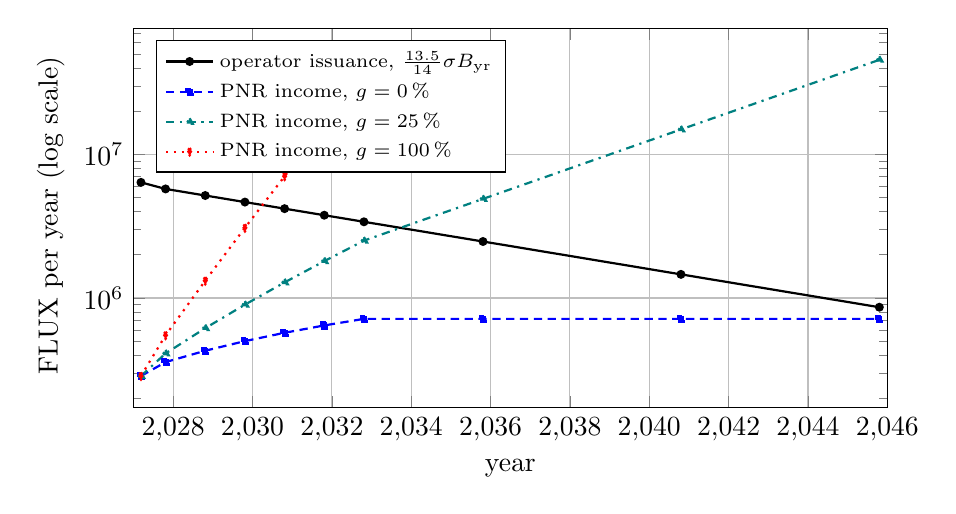
\begin{tikzpicture}
\begin{axis}[
  width=0.92\linewidth, height=6.4cm,
  xlabel={year},
  ylabel={\flux\ per year (log scale)},
  ymode=log,
  xmin=2027, xmax=2046,
  legend pos=north west,
  legend cell align=left,
  legend style={font=\scriptsize},
  grid=major,
  every axis plot/.append style={thick},
]
\addplot[black,mark=*,mark size=1.2pt] coordinates {
  (2027.19,6386040) (2027.81,5747436) (2028.81,5172692) (2029.81,4655423)
  (2030.81,4189881) (2031.81,3770893) (2032.81,3393803) (2035.81,2474083)
  (2040.80,1460921) (2045.80,862659)};
\addlegendentry{operator issuance, $\tfrac{13.5}{14}\subsidy\blocksyear$}
\addplot[blue,densely dashed,mark=square*,mark size=1.1pt] coordinates {
  (2027.19,286320) (2027.81,357900) (2028.81,429480) (2029.81,501060)
  (2030.81,572640) (2031.81,644220) (2032.81,715800) (2035.81,715800)
  (2040.80,715800) (2045.80,715800)};
\addlegendentry{\PNR income, $g=\SI{0}{\percent}$}
\addplot[teal,dashdotted,mark=triangle*,mark size=1.3pt] coordinates {
  (2027.19,286320) (2027.81,411010) (2028.81,616517) (2029.81,899102)
  (2030.81,1284395) (2031.81,1806178) (2032.81,2508521) (2035.81,4899436)
  (2040.80,14918700) (2045.80,45546000)};
\addlegendentry{\PNR income, $g=\SI{25}{\percent}$}
\addplot[red,dotted,mark=diamond*,mark size=1.3pt] coordinates {
  (2027.19,286320) (2027.81,550090) (2028.81,1320222) (2029.81,3081018)
  (2030.81,7041655) (2031.81,15844590) (2032.81,35210000)};
\addlegendentry{\PNR income, $g=\SI{100}{\percent}$}
\end{axis}
\end{tikzpicture}
\caption{Crossover in \flux terms \planned. Operator issuance falls on the reduction grid while the
operator share $\nodeshare$ ramps from $0.20$ to the cap $\nodesharecap = 0.50$; \PNR income is
$\nodeshare(\hgt)\,V_0(1+g)^{t}$. The $g = \SI{0}{\percent}$ series flattens at
$715{,}800\flux$ per year and never meets the issuance curve, whose perpetual tail is
$862{,}659\flux$ per year. Price does not appear on either axis and no price claim is made.}
\label{fig:pnr:crossover}
\end{figure}

\begin{remark}[Figure provenance]
The coordinates plotted in Figures~\ref{fig:pnr:crossover} and~\ref{fig:pnr:real} are the tabulated
output of \texttt{scripts/\allowbreak{}07-pnr-settlement.\allowbreak{}py} (run 2026-09-03), which also wrote
\texttt{paper/\allowbreak{}data/\allowbreak{}pnr\_crossover.\allowbreak{}dat} and \texttt{paper/\allowbreak{}data/\allowbreak{}pnr\_crossover\_real.\allowbreak{}dat}. Every
plotted point in Figure~\ref{fig:pnr:crossover} has been checked against the corresponding row of
that data file and agrees exactly; the data files carry their own \texttt{\#} provenance headers and
the figures are reproducible from them.
\end{remark}

\subsubsection{Real terms (secondary, price exogenous)}
\label{sec:pnr:real}

The \flux-denominated price table is revised by policy, and the revisions have historically tracked
real cost: the CPU rate has fallen $100\times$ across five revisions \shipped
\srcmeasured{api.runonflux.io/\allowbreak{}apps/\allowbreak{}deploymentinformation}{2026-09-03}. Under a continuation of that
rebasing policy, \flux inflow to the pool would be real demand divided by an exogenous price multiple,
$V^{\flux}_t = V_0(1+g)^{t}/m_t$, while issuance is fixed in \flux. Treating $m$ as an axis and not
as a forecast gives the following years-to-parity after activation.

\begin{table}[H]
\centering
\small
\begin{tabular}{lrrrrr}
\toprule
real growth $g$ $\backslash$ price multiple $m$ & $0.5$ & $1$ & $2$ & $5$ & $10$\\
\midrule
\SI{0}{\percent}   & $14.6$ & never & never & never & never\\
\SI{10}{\percent}  & $7.6$  & $11.6$ & $14.6$ & $19.6$ & $26.1$\\
\SI{25}{\percent}  & $5.6$  & $6.6$  & $9.6$  & $11.6$ & $13.6$\\
\SI{50}{\percent}  & $3.6$  & $4.6$  & $5.6$  & $7.6$  & $9.6$\\
\SI{100}{\percent} & $2.6$  & $3.6$  & $4.6$  & $5.6$  & $5.6$\\
\bottomrule
\end{tabular}
\caption{Years from activation to \flux-terms parity, as a function of real demand growth $g$ and an
exogenous price multiple $m$ \planned. $m$ is a sensitivity axis, not a projection.
Source: \texttt{paper/\allowbreak{}data/\allowbreak{}pnr\_crossover\_real.\allowbreak{}dat}.}
\label{tab:pnr:real}
\end{table}

\begin{figure}[H]
\centering
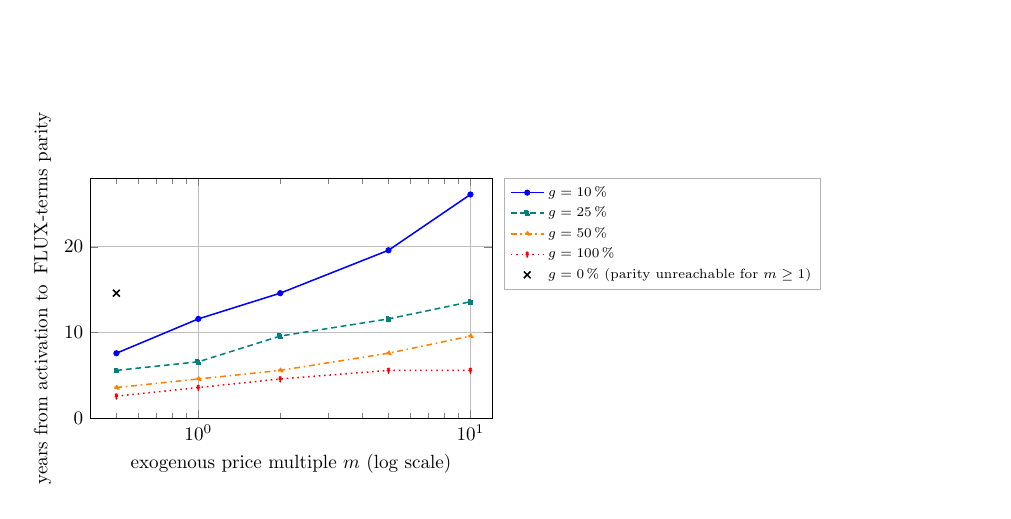
\begin{tikzpicture}
\begin{axis}[
  width=0.74\linewidth, height=6.0cm,
  xlabel={exogenous price multiple $m$ (log scale)},
  ylabel={years from activation to \flux-terms parity},
  xmode=log,
  log basis x=10,
  xmin=0.4, xmax=12,
  ymin=0, ymax=28,
  legend cell align=left,
  %% Outside the plot box: at north west the g=10% series ran straight through it.
  legend style={at={(1.03,1)}, anchor=north west, font=\scriptsize, draw=black!30},
  grid=major,
  every axis plot/.append style={thick},
]
\addplot[blue,mark=*,mark size=1.2pt] coordinates {
  (0.5,7.6) (1,11.6) (2,14.6) (5,19.6) (10,26.1)};
\addlegendentry{$g=\SI{10}{\percent}$}
\addplot[teal,densely dashed,mark=square*,mark size=1.1pt] coordinates {
  (0.5,5.6) (1,6.6) (2,9.6) (5,11.6) (10,13.6)};
\addlegendentry{$g=\SI{25}{\percent}$}
\addplot[orange,dashdotted,mark=triangle*,mark size=1.3pt] coordinates {
  (0.5,3.6) (1,4.6) (2,5.6) (5,7.6) (10,9.6)};
\addlegendentry{$g=\SI{50}{\percent}$}
\addplot[red,dotted,mark=diamond*,mark size=1.3pt] coordinates {
  (0.5,2.6) (1,3.6) (2,4.6) (5,5.6) (10,5.6)};
\addlegendentry{$g=\SI{100}{\percent}$}
\addplot[black,only marks,mark=x,mark size=2.5pt] coordinates {(0.5,14.6)};
\addlegendentry{$g=\SI{0}{\percent}$ (parity unreachable for $m \ge 1$)}
\end{axis}
\end{tikzpicture}
\caption{Real-terms sensitivity \planned, secondary analysis. Reading, and it is the point of the
figure: under a rebasing price policy, \emph{price appreciation delays \flux-terms parity} --- every
curve rises to the right. Appreciation can raise operator income in real terms while the
\flux-denominated ratio barely moves. The two statements live in different denominations and must
never be used to defend one another.}
\label{fig:pnr:real}
\end{figure}

\settlednote{Trailing receipts at $\mathsf{sink}$ (\Cref{tab:pnr-recommended}). O17 --- the measured revenue baseline that should replace ``$100\flux$ per application per
month''. Domain: $\{\text{trailing receipts at the payment sink } \texttt{t3Nryf\ldots}$,
$\text{list-price value of the measured resource totals}\}$; the census gives $8{,}972$ vCPU,
$17{,}544{,}229$~MB of RAM and $160{,}107$~GB of disk across $7{,}486$ instances
\srcmeasured{api.runonflux.io/\allowbreak{}apps/\allowbreak{}globalappsspecifications}{2026-09-03}. Every absolute figure in
this subsection scales linearly with it; the growth-rate conclusions do not.}

\settlednote{Rule-based rebasing (\Cref{tab:pnr-recommended}). The
decision is that rebasing follows a published rule rather than discretion or an oracle; the rule's
functional form is specified in \S\ref{sec:pnr:recommended} as trailing measured receipts adjusted at
fixed intervals, and its coefficients are a policy calibration rather than a mechanism choice. O9 --- price-table rebasing policy. Domain: $\{\text{discretionary (today)},\
\text{rule-based},\ \text{USD oracle}\}$. A rule removes a Foundation lever over pool inflow; an
oracle adds a trust dependency that would need its own treatment. The existence of a
\texttt{getappspecsusdprice} work item suggests movement here.}

% ---------------------------------------------------------------------------
\subsection{Open parameters}
\label{sec:pnr:openparams}

Of the twenty decisions this specification opened, four are now settled and are recorded in
Table~\ref{tab:pnr:closed}; the settlement decision created one more, O21, which \Cref{rem:pnr:o21} settles. Eleven more are
settled by the author's confirmation of \Cref{tab:pnr-recommended}, and O16 by \Cref{rem:o16-burn}; four therefore
remain open (O4, O8, O14 and O19), and the load-bearing one among them is \textbf{O8} --- which payment channels must
settle through $\mathsf{sink}$ --- because every channel outside it is revenue the consensus split
never touches and the counter of Property~\ref{prop:pnr:supply} never sees. None of the open values
is guessed anywhere in this section, and none of the closed ones is stated without its provenance.

\begin{table}[H]
\centering
\scriptsize
\begin{tabular}{llp{0.42\linewidth}l}
\toprule
id & decision & settled value & provenance\\
\midrule
O1 & drip constant $\drip$ & $86{,}400$ blocks, i.e.\ exactly \SI{30}{\day} at \SI{30}{\second} & \srcintent{evidence/design/08-answers-round-2.md}\\
O2 & commitment of $\pool_\hgt$ & committed in the coinbase (PC) and recomputed by every validator; no separate store, no header field & \srcintent{evidence/design/08-answers-round-2.md}, \srcdoc{plan/conflicts.md C37}\\
O3 & memo semantics & \texttt{OP\_RETURN} binding $H(m_\app)$, carried and not interpreted by consensus (PS2) & \srcintent{evidence/design/08-answers-round-2.md}\\
O18 & serialisation and enforcement boundary & one output of the full price to $\mathsf{sink}$ (PS1); consensus applies the split (PS4); \FluxOS checks only existence, memo and coverage & \srcintent{evidence/design/08-answers-round-2.md}, \srcdoc{plan/conflicts.md C36, C38}\\
\bottomrule
\end{tabular}
\caption{Decisions closed since the first draft of this specification \planned. All four are team
ratifications: O2 originated as this specification's recommendation and was subsequently adopted.
Each would be a consensus rule once activated, so changing any of them afterwards would be a network
upgrade.}
\label{tab:pnr:closed}
\end{table}

\begin{table}[H]
\centering
\scriptsize
\begin{tabular}{llp{0.30\linewidth}p{0.34\linewidth}}
\toprule
id & decision & domain & trade-off\\
\midrule
O4 & fee floor and spam resistance & $p_{\min} \ge 0.01\flux$; per-instance or per-deployment & dust-priced deployments contribute nothing yet occupy capacity; a floor prices out the micro-workloads \S18 wants\\
O5 & $D_{\hgt,t}$ with no payee in tier $t$ & stays in pool; dev fund; other tiers & pool: conservation-trivial; dev fund: one rule for subsidy and drip; other tiers: rewards concentration\\
O6 & partition residue $\epsilon_\hgt$ & pool; dev fund & $\le 2\sat$ per block either way; must be fixed to avoid divergence\\
O7 & shielded payers & transparent value required; Sapling with revealed amount; excluded & consensus needs the received value for PS4; the hide-payer/reveal-amount construction is \S21's\\
\textbf{O8} & scope of payments required to settle at $\mathsf{sink}$ & new deployments; renewals; credit top-ups (\S16); \CumulusVPN; enterprise & every excluded channel is revenue outside the consensus split and invisible to the revenue counter\\
O9 & price-table rebasing & discretionary; rule-based; USD oracle & a rule removes a Foundation lever; an oracle adds a trust dependency\\
O10 & drip ordering & from $\pool_{\hgt-1}$; after applying $F_\hgt$ & parent-state: coinbase checkable early, producer cannot influence own drip; post-inflow: one block less lag, same-block recapture returns\\
O11 & initial seed $\pool_{\hpa-1}$ & $0$; Foundation-funded seed & seed removes the $\sim$90-day ramp but is a one-off transfer and must be labelled one\\
O12 & fleet-growth guard on $\drip$ & none; documented hard-fork review trigger & at $4\times$ Cumulus the spread is \SI{16}{\percent}; an automatic rule is a manipulation surface\\
O13 & ramp policy if demand undershoots & fixed schedule; a stated revision process & with $g=0$ there is no crossover; the schedule's behaviour is unstated\\
O14 & identity of $\mathsf{sink}$ & keep \texttt{t3Nryf\ldots}; a fresh address; rotation/PQ path (\S8) & keeping it preserves tooling and one continuous history but mixes pre-$\hpa$ spendable receipts into the counter; a consensus-level address is a consensus-level commitment and rotation is a hard fork absent a mechanism\\
O15 & emergency blocks and the drip & $D_\hgt = 0$ (required, S1); normal drip & otherwise 2-of-4 keys, facing no time gating, can accelerate the release of accumulated fees\\
O16 & forfeited tenant balances (\S23) & anywhere but $\pool$ (required, S2) & routing to the pool pays for report brigading\\
O17 & measured revenue baseline for $V_0$ & explorer receipts; list-price of measured resources & \S\ref{sec:pnr:crossover} scales linearly with it; closable by observation once $\mathrm{Rev}$ exists\\
O19 & tier partition basis & \PoN bases $1 : 3.5 : 9$ & confirm only; must not be described as collateral-proportional (Remark~\ref{rem:pnr:c24})\\
O20 & PA cut applied uniformly & uniform $\times 1/2$; other & changes operator issuance and every parity figure\\
\bottomrule
\end{tabular}
\caption{Parameters of the \PNR settlement mechanism, after the closures of
Table~\ref{tab:pnr:closed}; the values since settled are in \Cref{tab:pnr-recommended}, and O4, O8,
O14 and O19 remain open. The bold row is the one that gates the rest. Mirrored in
\texttt{plan/\allowbreak{}decisions-needed.\allowbreak{}md}.}
\label{tab:pnr:open}
\end{table}

Three requirements are exported to other mechanisms and are restated here so that they are not lost
at a section boundary: to \S16, \emph{every application-hosting charge, whatever the payment channel,
settles as exactly one L1 payment to $\mathsf{sink}$, or the consensus split is void and the revenue
counter under-reports}; to \S23,
\emph{forfeited balances never enter $\pool$} (Property~\ref{prop:pnr:exported}, S2); and to \S14,
\emph{the eligibility gate admitting a node to $\payees$ must be hosting-conditioned}
(Open Problem~\ref{op:pnr:d1}).

% ---------------------------------------------------------------------------
\subsection{Recommended values for the remaining open parameters}
\label{sec:pnr:recommended}

Each parameter still open above is given a recommended value here, with the reasoning that produced
it. Each was proposed by this paper and \textbf{confirmed by the author}
\srcintent{08-answers-round-2.md, round 11}, and several are simply a
recommendation to keep the default that \Cref{def:pnr:pool} already takes --- which is worth stating
explicitly, because a default that nobody has ratified is not the same object as a default that has
been examined and kept.

\begin{table}[H]
\centering\footnotesize
\caption{Values for the open \PNR{} parameters. Proposed by this paper and \textbf{confirmed by the
author} \srcintent{08-answers-round-2.md, round 11}. \planned, \srcinferred{} for the derivations.}
\label{tab:pnr-recommended}
\begin{tabular}{@{}llp{0.46\linewidth}@{}}
\toprule
& \textbf{Recommended} & Reason \\
\midrule
O5 tier with no confirmed node & \textbf{stays in $\pool$} & conservation-trivial; self-correcting
when that tier next confirms \\
O6 partition residue & \textbf{stays in $\pool$} & \num{0.021}\flux/year does not justify dev-fund
plumbing \\
O7 shielded payers & \textbf{moot} & pools retired; all settlement transparent
(\Cref{rem:o7-moot}) \\
O9 price rebasing & \textbf{rule-based} & removes a Foundation lever without adding an oracle
dependency \\
O10 drip ordering & \textbf{from $\pool_{\hgt-1}$} & keep the default: coinbase checkable before the
block's own receipts \\
O11 initial seed & \textbf{0} & a seed is a one-off Foundation transfer to operators \\
O12 fleet-growth guard & \textbf{review trigger at $2\times$} & documented, not automatic \\
O13 undershoot policy & \textbf{fixed schedule $+$ stated review} & no silent re-cutting \\
O15 emergency blocks & \textbf{$D_\hgt = 0$} & required by S1 \\
O17 revenue baseline & \textbf{trailing sink receipts} & measured, not assumed \\
O20 halving uniformity & \textbf{uniform $\times 1/2$} & every parity figure in
\S\ref{sec:pnr:crossover} assumes it \\
\bottomrule
\end{tabular}
\end{table}

\paragraph{The three that are not housekeeping.}

\textbf{O11, no seed.} Seeding $\pool_{\hpa-1}$ above zero would remove the ninety-day ramp and give
operators income from the first post-activation block. It would also be a one-off Foundation transfer
to node operators, and it would have to be described as one --- in a section whose entire argument is
that \PNR{} replaces issuance with demand-side revenue. Starting at zero makes the ramp visible and
makes the first ninety days an honest measurement of whether demand exists. If the ramp is judged too
harsh, the correct instrument is the activation schedule, not a subsidy that muddies what the pool
balance means.

\textbf{O9, rule-based rebasing.} The price table is today a Foundation lever over pool inflow with
no consensus involvement, which sits awkwardly beside a mechanism whose legitimacy rests on operators
being paid from receipts rather than from discretion. Of the three options, an oracle imports a trust
dependency that would need its own threat model and its own section; discretion preserves the lever.
A rule --- rebasing on a published function of trailing measured receipts, adjusted at fixed
intervals --- removes the lever without adding a dependency, and it is the only option under which a
tenant can predict next period's price from public data. What the rule should be is left open; that
it should be a rule is the recommendation.

\textbf{O17, trailing receipts rather than list-price value.} The placeholder baseline of
``\num{100}\flux{} per application per month'' should be replaced by the trailing receipts actually
observed at $\mathsf{sink}$, not by the list-price value of the measured resource totals. The two
differ by exactly the utilisation gap, and \S\ref{sec:limitations} records that realised utilisation
is not measurable from public data. A baseline computed from list prices would therefore embed an
unmeasured assumption in the one number the crossover analysis is most sensitive to, and would do so
invisibly. Trailing receipts are smaller, real, and reproducible by anyone watching the sink address.

\subsection{Comparison with prior art}
\label{sec:pnr:related}

\begin{table}[H]
\centering
\scriptsize
\begin{tabular}{lp{0.16\linewidth}p{0.16\linewidth}p{0.38\linewidth}}
\toprule
system & who is paid & from what & what \Flux would do differently\\
\midrule
Ethereum, post-EIP-1559 & block proposer (priority fee); base fee burned & per-transaction fee, same block & no burn; the operator share is pooled and dripped to \emph{all} nodes through the rotation, and a producer gains nothing by including a payment. The same-block capture EIP-1559 grants the proposer by design is precisely what Theorem~\ref{thm:pnr:timing} removes\\
Filecoin \citep{filecoin2017} & the specific storage provider & per-deal escrow released on proof of storage, with slashing & payment strictly conditional on proven service there; unconditional and network-wide here (H4, P7). \Flux would trade the proof-of-service dependency for fairness and simplicity, and inherit the free-rider problem of \S\ref{sec:pnr:hosting} in exchange\\
Akash \citep{akash} & the winning provider & tenant escrow drawn down per block at the bid price, with a take rate to a community pool & no per-lease escrow to the host and no auction; the network take would be \SIrange{80}{50}{\percent} to a Foundation address rather than a governance-controlled pool. Stated without softening\\
Render \citep{render} & node operators in proportion to work & burn-and-mint: payments burned, emissions minted to workers & burn-and-mint ties reward to metered work. The settled design rejects both the burn and the metering, which is exactly the roadmap model superseded by C1\\
Dash masternodes & one masternode per block, longest-since-paid queue & block subsidy plus a treasury share & the nearest structural precedent for Proposition~\ref{prop:pnr:rotation}; Dash never routed application fees through the rotation. \Flux would be that rotation plus a fee pool \srcdoc{plan/mech-pnr.md \S9}\\
Cosmos SDK \texttt{x/distribution} & all validators in proportion to stake, every block, lazily accumulated & transaction fees, with a community tax & exact and immediate, but requires per-validator accumulators and withdraw transactions. \Flux would pay through three existing coinbase outputs with no per-node state and no claim transaction (P4, P5), accepting a bounded \SI{3.83}{\percent} spread and a twenty-day lag instead. This is the road not taken \srcdoc{plan/mech-pnr.md \S9}\\
\bottomrule
\end{tabular}
\caption{\PNR against fee-handling and work-payment prior art.}
\label{tab:pnr:related}
\end{table}

The combination specific to \Flux is: coinbase-only payment with no per-node accounting; a
deterministic rotation that makes network-wide distribution provably fair over one rotation
(Propositions~\ref{prop:pnr:rotation} and~\ref{prop:pnr:within}); and a proportional drip with no
epoch boundary (Property~\ref{prop:pnr:invariants}, I3) that converts a schedule everyone can read
into a schedule nobody can profit from reading (Theorem~\ref{thm:pnr:timing}). The cost is stated
once more because it is the design's real weakness, and because \S\ref{sec:feasibility} and \S\ref{sec:migration} both depend on it:
\textbf{\PNR would pay for membership, and membership is only as real as the gate}.

%% Drain this section's float queue before the next begins.
\FloatBarrier

\section{Chain operations and evolution: main-chain pruning, collateral maturity, and post-quantum migration}
\label{sec:chain-evolution}\label{sec:chain-ops}

The roadmap groups three chain-level changes under a single H1 2027 heading, and a reader could be
forgiven for assuming they are equally ready because they share a quarter
\srcroadmap{H1 2027 chain-changes section}. They are not. One of them, main-chain pruning, is
already-shipped software wired into \fluxd; the operational decision is what is new. The second,
collateral maturity, is a named consensus-rule proposal with an explicit open item that decides
whether it works at all. The third, post-quantum migration, has a deliverable for H1 2027 that is a
published plan, not a change to any key. This section keeps the three separate, states a maturity
tag and a feasibility class for each, and closes with the constraint all three share: none of them can
rotate a key the protocol does not itself control. Collateral maturity delays when an existing key may
spend; it does not replace that key. Post-quantum migration is precisely the case in which the
protocol would like to replace a key and structurally cannot without the key-holder's cooperation.

\begin{figure}[H]
\centering
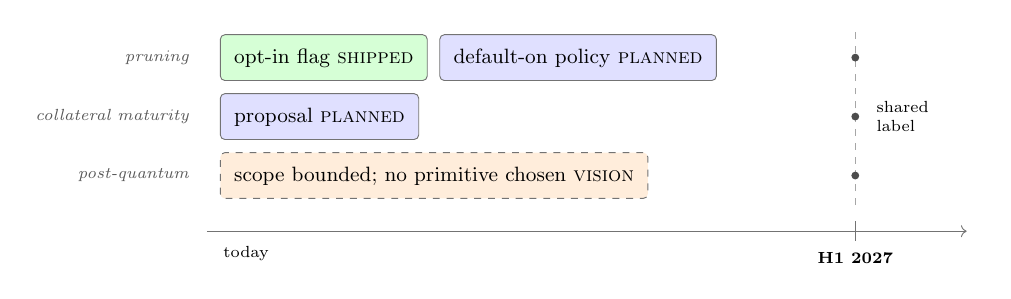
\begin{tikzpicture}[font=\small,
  track/.style={rounded corners=2pt, minimum height=7mm, text height=1.6ex, text depth=.4ex,
                draw=black!55, inner xsep=6pt},
  ship/.style={track, fill=green!16},
  plan/.style={track, fill=blue!12},
  vis/.style={track, fill=orange!14, dashed},
  lbl/.style={font=\scriptsize\itshape, text=black!65},
]
% shared time axis
\draw[->, black!55] (0,-0.1) -- (11.6,-0.1);
\node[font=\scriptsize, anchor=north] at (0.6,-0.2) {today};
\draw[black!55] (9.9,0.05) -- (9.9,-0.25);
\node[font=\scriptsize\bfseries, anchor=north] at (9.9,-0.3) {H1 2027};

% pruning
\node[lbl, anchor=east] at (-0.15,2.55) {pruning};
\node[ship, anchor=west, minimum width=2.9cm] at (0.2,2.55) {opt-in flag \shipped};
\node[plan, anchor=west, minimum width=3.4cm] at (3.55,2.55) {default-on policy \planned};

% collateral maturity
\node[lbl, anchor=east] at (-0.15,1.65) {collateral maturity};
\node[plan, anchor=west, minimum width=2.2cm] at (0.2,1.65) {proposal \planned};

% post-quantum
\node[lbl, anchor=east] at (-0.15,0.75) {post-quantum};
\node[vis, anchor=west, minimum width=5.4cm] at (0.2,0.75) {scope bounded; no primitive chosen \vision};

% the shared marker
\draw[black!35, dashed] (9.9,0.3) -- (9.9,3.0);
\foreach \y in {2.55,1.65,0.75} \fill[black!70] (9.9,\y) circle (1.7pt);

\node[anchor=west, font=\scriptsize, text width=1.5cm, align=left] at (10.1,1.65)
  {shared \\ label};
\end{tikzpicture}
\caption{Three chain-evolution tracks that the roadmap places under one ``H1 2027'' label, shaded by
\emph{maturity} rather than by calendar position. The label is shared; the readiness is not. Pruning
exists as an opt-in flag today and needs a policy decision to become a default; collateral maturity is
a proposal with no code path in \fluxd yet; post-quantum migration has a bounded scope and no chosen primitive, and is the only
one of the three whose hardest sub-problem (\Cref{rem:pq-disposition}) is unsolved industry-wide. A
reader who takes the shared date as shared readiness would mis-plan all three.}
\label{fig:chain-evolution-tracks}
\end{figure}

\subsection{Main-chain pruning: an operational decision, not a new capability}

\texttt{-prune} is standard, inherited Bitcoin/Zcash functionality and is fully wired in \fluxd today
\shipped\ \srccode{fluxd/\allowbreak{}src/\allowbreak{}init.cpp}{986--1064, 1919} \srccode{fluxd/\allowbreak{}src/\allowbreak{}main.cpp}{4312--4313, 5930}.
\texttt{n\allowbreak{}Prune\allowbreak{}After\allowbreak{}Height} is set to $100{,}000$ on mainnet \srccode{fluxd/\allowbreak{}src/\allowbreak{}chainparams.cpp}{181}. No
\PoN-specific pruning constraint was found in the code. So ``main-chain pruning'' as a roadmap item is
not the implementation of a new capability; it is the decision to turn on a capability that already
exists, together with the archival tier that has to sit beside it once history is no longer kept by
every node \srcroadmap{Main-chain pruning, H1 2027}.

The roadmap's own justification is that pruned nodes remain able to produce blocks:

\begin{quote}
``30-second blocks mean the chain grows quickly. Pruning cuts what a node must store and speeds up
syncing. Done properly, pruned nodes stay fully able to produce blocks, with designated archive nodes
preserving full history for explorers and the data services above.''
\srcdoc{flux-roadmap-public.md:121-122}
\end{quote}

Under \PoN\ this is a claim worth proving rather than restating, because block production requires two
things that a naive reading of ``pruning'' might endanger: evaluating slot eligibility
$H(\text{collateral} \Vert \text{prevHash} \Vert \tslot) \le \text{target}$ and signing
\srccode{fluxd/\allowbreak{}src/\allowbreak{}pon/\allowbreak{}pon.cpp}{70--86}, and validating the \FluxNode\ registry against which that
collateral outpoint is checked. The reason the claim holds is that the registry does not live inside
the block store it would otherwise be pruned along with: \FluxNode\ state is a single global structure,
\texttt{g\_fluxnode\allowbreak{}Cache}, persisted in its own LevelDB database keyed by datadir path
\texttt{determ\_zelnodes} \srccode{fluxd/\allowbreak{}src/\allowbreak{}fluxnode/\allowbreak{}fluxnodecachedb.cpp}{26}, and is rebuilt from that
store at every startup independently of how much of the block chain is retained
\srccode{fluxd/\allowbreak{}src/\allowbreak{}fluxnode/\allowbreak{}fluxnodecachedb.cpp}{49--79}.

\begin{property}
A pruned \PoN\ node retains block-production capability if and only if the \FluxNode\ registry and the
UTXO set for collateral outpoints are retained, regardless of pruning depth.
\end{property}

This is stateable precisely because the registry already lives outside the block store rather than
being derived from block history on demand; a chain whose node registry had to be replayed from full
block history would not have this property, and \fluxd's separation of the two stores is what makes
pruning and \PoN\ compatible without further engineering \shipped\
\srccode{fluxd/\allowbreak{}src/\allowbreak{}fluxnode/\allowbreak{}fluxnodecachedb.cpp}{26,49--79}.

\begin{remark}[Archival is a tenant product, not a node obligation --- settled]
\label{rem:archive-product}
The pruning-depth policy and the archival-redundancy target were carried as open. They are settled by
a decision that resolves both at once and relocates the problem: \textbf{archive nodes are
applications running on \FluxCloud}. The team deploys them as tenant workloads and sells access to
RPC and other node APIs as a product \srcintent{08-answers-round-2.md, round 16} (\planned).

Two consequences, and the second is the one worth stating carefully.

\emph{Pruning is unconstrained by any retention obligation.} If no node is obliged to keep history,
the pruning-depth policy is a storage-efficiency choice for ordinary operators rather than a
network-safety parameter, and it can be set as aggressively as operators want. The awkward coupling
that made this an open question --- how deep can we prune without endangering history --- dissolves,
because history is not being kept by the pruning nodes in the first place.

\emph{History availability becomes a function of demand for a product.} This is the honest form of
the trade and the paper states it plainly: if archival capacity is a paid service, then history
survives exactly as long as someone finds it worth paying for. That is a different guarantee from
``every node keeps everything'', and it is weaker in a specific way --- there is no protocol rule
setting a minimum number of archive nodes, so the redundancy target is a commercial decision, not a
consensus one. A chain whose full history rests on the commercial viability of an archive product
should say so, and this one does.
\notestablished{no redundancy target for archive deployments is stated in any artefact read
for this paper, and none is derivable from the decision that archival is a product. The number of
independent archive deployments required before history is durable is therefore not stated here.}
\end{remark}

The roadmap pairs pruning with a paid product built from the archive nodes pruning requires, describing
RPC, archive and indexing services as the network's ``first capacity-selling product'' and stating that
this ``pairs directly with chain pruning: the archive nodes pruning requires become the product''
\srcdoc{flux-roadmap-public.md:33-34}. This is the clearest instance in the deployed system of the
demand-funded thesis applied to the chain layer itself: an operational cost the network would otherwise
carry for free (full history) becomes a service the network sells, and the archive tier pruning makes
necessary is the same tier that generates the revenue. \srcroadmap{RPC, archive and indexing services,
Q3 2026}

See \Cref{rem:archive-product}: archival capacity \emph{is} a paid product, deployed as
\FluxCloud{} applications, and the consequence for history availability is stated there rather than
left conditional. \srcinferred

\textbf{Class: Extension.} The mechanism exists; what remains is the operational decision to enable it
and the archival-capacity policy above.

\subsection{Collateral maturity: a proposal, not yet a rule}

Collateral maturity is not deployed and has no code path in \fluxd today; the roadmap presents it
explicitly as a proposal that has not yet gone to operators \srcroadmap{Collateral maturity, H1 2027}
\planned. The stated rule is a rolling maturity on the collateral outpoint, modelled on coinbase
maturity:

\begin{quote}
``For attestation to carry real weight, a node's stake in the network has to outlast the window in
which its claims can be challenged. We will propose a consensus rule: a node-collateral UTXO becomes
spendable only 30 days after the node's last confirmed activity — a rolling maturity, like coinbase
maturity, applied prospectively and never to standing collateral. Moving collateral directly into a new
or upgraded node (including into multisig custody) stays instant; only leaving waits. There is no
confiscation and never will be.'' \srcdoc{flux-roadmap-public.md:143-144}
\end{quote}

Formally: for a collateral outpoint $o$ with last confirmed activity height $\hgt_{\mathrm{act}}(o)$,
spending $o$ would be valid at height $\hgt$ if and only if
\[
\hgt \;\ge\; \hgt_{\mathrm{act}}(o) + M
\qquad\text{or}\qquad
\mathrm{dest}(o) \in \mathcal{D}_{\text{node}},
\]
with $M = 86{,}400$ blocks — 30 days at the \PoN\ target spacing $\spacingpon = 30\,\mathrm{s}$ — and
$\mathcal{D}_{\text{node}}$ the set of destinations that constitute continued participation.

\notestablished{the definition of $\mathcal{D}_{\text{node}}$ --- which destinations count as
continued participation, so that a move into a new or upgraded node or into multisig custody stays
instant while an exit disguised as a move does not --- is stated in no artefact read for this paper.
It is the parameter on which the rule's acceptability rests: too permissive and the rule does
nothing, too restrictive and funds are held by a mechanism promised not to hold them.}

\proposednote{$M = \num{86400}$ blocks is this paper's recommendation, and the constraint that made
it non-free-standing is satisfiable: it must satisfy $M \ge \Delta_{\mathrm{chal}}$, and
\S\ref{sec:attested-execution} recommends $\Delta_{\mathrm{chal}} = \num{2880}$ blocks. With
$\num{86400} \ge \num{2880}$ the constraint holds with a factor of \num{30} in hand, so $M$ can be
treated as a free choice after all --- and it reuses the \PNR{} constant $K$, so one number serves
three mechanisms. \srcinferred.}

Non-retroactivity is stated as part of the proposal and is what makes it non-confiscatory:

\begin{property}
For every collateral outpoint existing before the activation height $\hgt_{\mathrm{act}}^{\star}$, the
maturity rule does not apply: no standing collateral is retroactively locked.
\end{property}

The roadmap also states a second-order effect openly rather than leaving it to be found later — a
maturity rule smooths collateral unlock waves — and frames this as a proposal that would ride an
already-planned network upgrade rather than force its own:

\begin{quote}
``We state the second-order effect ourselves rather than leaving it to be discovered: a maturity rule
also smooths collateral unlock waves. Both effects are the point. This is a proposal — it goes to
operators for discussion before any activation is scheduled, and it would ride an already-planned
network upgrade rather than forcing its own.'' \srcdoc{flux-roadmap-public.md:146}
\end{quote}

Stated honestly, the rule buys a bounded window rather than permanence: an operator willing to stop
operating and wait $M$ blocks can still exit with the collateral intact, exactly as before the rule
existed. What the maturity rule changes is the cost of lying about continued participation while
attempting to exit early; what makes lying about an attestation claim actually costly is the bond
described in Section~14, not the maturity window itself. Section~8 and Section~14 divide the labour
this way: the maturity window guarantees stake outlasts a challenge; the bond is what is at risk if the
challenge succeeds.

\textbf{Class: Engineering.} There is no unsolved technical problem in the maturity rule as stated; the
open item is the definition of $\mathcal{D}_{\text{node}}$, and the real cost is the political work of
operator consent the roadmap itself names as a prerequisite \srcroadmap{Collateral maturity, H1 2027}.

\subsection{Post-quantum migration: a scope decision and an open problem}

The H1 2027 deliverable is a published migration path, not a migration:

\begin{quote}
``The realistic threat is store-now-decrypt-later, not live breakage. We publish a migration path on
the NIST-standardised signature schemes. Migration itself is a multi-year effort — this is where
Bitcoin and Ethereum are too.'' \srcdoc{flux-roadmap-public.md:148-149}
\end{quote}

\vision\ \srcroadmap{Post-quantum roadmap, H1 2027}. Consistent with that, a repository-wide grep for
the obvious primitive names returns nothing: \srccode{fluxd/\allowbreak{}src}{repo-wide grep for
\texttt{quantum|dilithium|kyber|falcon|sphincs|schnorr}: zero hits outside a vendored
\texttt{secp256k1/\allowbreak{}.\allowbreak{}gitignore}}. No post-quantum code, comment, or dependency exists in \fluxd\ today.

\paragraph{What is at risk.} The signature primitives at risk are all classical-ECDSA over
secp256k1: transparent-address spending; \FluxNode\ registration and confirmation signing, via
\texttt{Sign\allowbreak{}Deterministic\allowbreak{}Start\allowbreak{}Tx} and \texttt{Build\allowbreak{}Deterministic\allowbreak{}Confirm\allowbreak{}Tx}
\srccode{fluxd/\allowbreak{}src/\allowbreak{}fluxnode/\allowbreak{}activefluxnode.cpp}{253--288,380--407}; the \PoN\ block header's own
\texttt{vchBlockSig} field, an ECDSA signature over the block hash carried in every post-activation
header alongside the winning collateral outpoint \srccode{fluxd/\allowbreak{}src/\allowbreak{}primitives/\allowbreak{}block.h}{44--45,64--96};
the 2-of-4 emergency-block key set \srccode{fluxd/\allowbreak{}src/\allowbreak{}chainparams.cpp}{242--253}; and the
benchmark-signing key allowlist \srccode{fluxd/\allowbreak{}src/\allowbreak{}chainparams.cpp}{233--240}, alongside the
attestation-signing keys discussed in Section~14. Hashing is a separate matter: SHA-256 and the
historical chain's Equihash instantiation degrade only quadratically under a quantum adversary, which
is a general property of quantum search against hash-based primitives rather than a Flux-specific
finding, and is not the part of the system this scope decision needs to address \srcinferred.

\paragraph{The scope decision.} The team has settled, as design intent, that the post-quantum scope is
deliberately bounded to consensus, transparent transactions, and the keys securing them, with the
shielded layer explicitly excluded and deferred as the field matures, on the grounds that privacy is
optional on \Flux\ and the transparent layer is the one every user and every consensus rule depends on
\srcintent{05-privacy-pq.md} \vision. This is presented as a considered position, not a gap, and it
carries a consequence the paper states plainly because a reviewer would otherwise find it: Groth16, the
proving system underlying the shielded pool described in Section~20, rests on a pairing assumption and
is not post-quantum secure. An unqualified ``quantum-ready \Flux'' claim made alongside a live shielded
pool built on Groth16 would therefore be an error; the bounded scope stated here is exactly what avoids
making it \srcintent{05-privacy-pq.md}.

\textbf{The retirement decision simplifies this considerably.} With both shielded pools retired
(\S\ref{sec:shielded-retirement}), Groth16 leaves the consensus path altogether, and with it the one
component whose presence made a ``quantum-ready \Flux'' claim require careful qualification. After
retirement the post-quantum scope is not \emph{bounded} to transparent transactions --- it is
\emph{coextensive} with the chain, because transparent transactions and the keys securing them are
all that remains. That is a genuine simplification of the migration problem stated in this section,
and it was not among the reasons given for the decision, which makes it worth recording as a
consequence rather than a justification.

A related and separate point, kept separate deliberately: adopting Halo2/Orchard-class proving would
remove the shielded layer's inherited trusted setup, which is a real, independently motivated
improvement discussed in Section~20 --- but it would not make the shielded pool post-quantum secure,
since Halo2 rests on discrete-log hardness rather than a quantum-hard assumption. Eliminating a trusted
setup and achieving post-quantum security are different properties, and this section, Section~14, and
Section~20 must not conflate them \srcintent{05-privacy-pq.md}.

\paragraph{The migration problem.} Signature migration on a UTXO chain is not an ordinary protocol
upgrade, because the protocol cannot move funds it does not hold the key to.

\begin{openproblem}
Let $U_{\mathrm{cls}}$ be the set of outputs spendable only by a classical signature. No consensus rule
can move an output in $U_{\mathrm{cls}}$ without the corresponding private key. A store-now-decrypt-later
adversary harvests public keys revealed at spend time and, once a capable quantum adversary exists,
spends any output in $U_{\mathrm{cls}}$ whose public key it has recorded. A migration must therefore
(i) offer a post-quantum output type, (ii) incentivize or compel movement of value into it, and
(iii) decide what happens to outputs in $U_{\mathrm{cls}}$ that never move.
\end{openproblem}

Item (iii) has no good answer anywhere in the industry today, and the honest statement is that \Flux\
is in the same position as Bitcoin and Ethereum, not ahead of them \srcdoc{flux-roadmap-public.md:149}.
The design space for the disposition of unmoved classical outputs has three known shapes, each with a
distinct trade-off:

\begin{enumerate}
\item \emph{A flag-day freeze.} After a fixed height, any output in $U_{\mathrm{cls}}$ whose owner has
not moved it becomes permanently unspendable. This forces the migration but is confiscatory by
construction for anyone who cannot act in time — lost keys, custodial delay, simple inattention — which
is exactly the property the collateral-maturity rule above was designed to avoid.
\item \emph{A permanent classical tail.} Nothing is ever frozen; the network accepts that any output in
$U_{\mathrm{cls}}$ whose public key becomes known remains at risk indefinitely once a capable adversary
exists. Nothing is confiscated, but the exposure never closes.
\item \emph{A hash-based commitment allowing a post-quantum proof of prior ownership.} An owner could
later prove, using a post-quantum-secure proof, that they controlled a given classical output before
some cutover, without needing a pre-committed post-quantum key at the time of the original output.
This is the least destructive of the three on its face, but so far as this section's sources establish,
no production-grade construction of this kind is deployed anywhere at the scale a base-layer chain
would require \srcinferred.
\end{enumerate}

\begin{remark}[\FluxNode{} collateral public keys are already public, by protocol design]
\label{rem:pq-collateral-exposed}
The three dispositions above are the general framing, and it is the framing Bitcoin and Ethereum
share. \Flux{} is not in the same position, and the difference is material enough that the
disposition question has to be answered per class rather than once.

On a Bitcoin-derived chain the structural mitigation for unmoved funds is that a P2PKH output commits
to $\mathsf{HASH160}(pk)$ rather than to $pk$: the public key is not on the chain until the output is
spent, so an adversary running Shor's algorithm has nothing to attack. That protection does not exist
for \FluxNode{} collateral. The \texttt{collateral\allowbreak{}Pubkey} field is serialised directly into the
\FluxNode{} START transaction and written to the chain at registration \shipped
\srccode{fluxd/src/primitives/transaction.h}{1038--1039};
\srccode{fluxd/src/fluxnode/activefluxnode.cpp}{368}. Every operating node has therefore
\emph{published} its collateral public key as a condition of operating, permanently and in the clear.

\begin{table}[H]
\centering\footnotesize
\caption{Collateral whose public keys are on-chain by protocol design. Node counts and tier split
\shipped \srcmeasured{\texttt{listzelnodes}}{2026-09-03}; supply from the emission model at height
\num{2912015}.}
\label{tab:pq-exposure}
\begin{tabular}{@{}lrrr@{}}
\toprule
Tier & Nodes & Collateral each (\flux) & Tier total (\flux) \\
\midrule
Cumulus & \num{3247} & \num{1000} & \num{3247000} \\
Nimbus & \num{1615} & \num{12500} & \num{20187500} \\
Stratus & \num{1627} & \num{40000} & \num{65080000} \\
\midrule
\textbf{Total} & \textbf{\num{6489}} & & \textbf{\num{88514500}} \\
\multicolumn{3}{@{}l}{Share of issued supply (\num{429466824}\flux)} & \textbf{\SI{20.61}{\percent}} \\
\bottomrule
\end{tabular}
\end{table}

\noindent \textbf{So roughly one fifth of issued supply sits in outputs that a cryptographically
relevant quantum computer could spend immediately}, without waiting for the owner to reveal anything,
and that fraction is not the result of user carelessness --- it is what the registration protocol
requires. This is a genuine architectural disadvantage relative to Bitcoin on this specific axis, and
the paper states it rather than inheriting Bitcoin's more comfortable framing.

\textbf{A correction this paper owes its own earlier reasoning.} An earlier draft concluded that
option (iii) --- a post-quantum proof of prior ownership --- was \emph{unavailable} for
\FluxNode{} collateral, on the argument that such a proof rests on the owner knowing a secret the
adversary cannot compute, which fails once $pk$ is published and Shor yields the private key. That
argument is wrong, and Bitcoin's own work shows why: the secret need not be the private key.
BIP-361 rests its rescue path on the knowledge asymmetry created by \textbf{BIP-32 hardened
derivation} \citep{bip361}. A hardened step derives the child key through a one-way function of the
parent seed, so recovering the child private key does not yield the seed. An owner can therefore
prove \emph{``I know a seed and a path that derive this key''} while a quantum adversary holding the
private key cannot. Option (iii) survives public-key exposure, provided the key was seed-derived
through a hardened step --- which is the normal case for wallet-generated keys and not the case for
raw imported ones.

So the design space for \FluxNode{} collateral does \emph{not} collapse to freeze-or-expose. It
collapses to something better, and \S\ref{sec:pq-frontier} builds on it.
\end{remark}

\subsection{The frontier: what Bitcoin is building, and the one move Flux can make that it cannot}
\label{sec:pq-frontier}

Bitcoin is the right comparison for this problem, because it faces the same one at larger scale and
its work is public, specified and adversarially reviewed. Two proposals define the current state of
that art, and \Flux{} should be read against them rather than against a generic notion of
``quantum readiness''.

\textbf{BIP-360} defines \emph{Pay-to-Merkle-Root} (P2MR): an output type offering nearly the
functionality of P2TR with the key-path spend removed, so that no internal public key is exposed and
a long-exposure attack by a cryptographically relevant quantum computer has nothing to work on. It is
Draft status, and it deliberately introduces \emph{no} post-quantum signature scheme --- the
algorithm choice is left to later work \citep{bip360}. \textbf{BIP-361} supplies the migration
policy: Phase~A, at \num{160000} blocks after activation, disallows sending funds \emph{to}
quantum-vulnerable addresses; Phase~B, two years later, tightens verification of ECDSA and Schnorr
signatures, freezing what has not moved. Its authors reject allowing theft outright, and its rescue
path rests on the hardened-derivation asymmetry described above --- with zk-STARK and commit-reveal
named as candidate proof systems and the honest admission that how much supply such a protocol could
cover ``remains to be seen'' \citep{bip361}. As of 2026-03-01, over \SI{34}{\percent} of all bitcoin
had revealed a public key on chain \srcinferred.

\paragraph{Where \Flux{} sits against that.} Two differences matter, and they point in opposite
directions.

\emph{Worse:} Bitcoin's exposed fraction is the product of user \emph{behaviour} --- spending, address
reuse --- and it grows monotonically because each spend reveals a key. \Flux's exposed fraction for
node collateral is the product of \emph{protocol mandate}: \SI{20.61}{\percent} of supply
(\Cref{tab:pq-exposure}) is exposed because the START transaction requires it, and an operator cannot
decline. No amount of careful user behaviour reduces it.

\emph{And a consequence Bitcoin's approach would not fix:} BIP-360's remedy is an output type that
hides the key in the \emph{scriptPubKey}. That does not help \Flux, because \Flux{}'s collateral
exposure is not in the output script at all --- it is in the \texttt{collateral\allowbreak{}Pubkey} field of the
\FluxNode{} transaction \srccode{fluxd/src/primitives/transaction.h}{1038--1039}. Adopting a
P2MR-equivalent output type would leave the exposure exactly where it is. \textbf{The registration
transaction format is what would have to change}, and that is a \Flux-specific problem with no
upstream solution to inherit.

\emph{Better, and decisively:} \textbf{\Flux{} has a mandatory, recurring, authenticated channel to
precisely the exposed set, and Bitcoin has none.} Bitcoin cannot reach a dormant holder; its only
instruments are to stop new exposure, to freeze, and to hope a rescue proof covers enough. Every
\Flux{} node, by contrast, must broadcast a START transaction to register and CONFIRM transactions to
keep being paid. The set with exposed keys \emph{is} the set transacting regularly and drawing income
--- and that turns an unreachable population into a reachable one.

\begin{remark}[Pre-staged commitment: the move the mandatory registration makes available]
\label{rem:pq-prestage}
The recommendation of \Cref{rem:pq-disposition} is eligibility-forced migration, and the team has
adopted it \srcintent{08-answers-round-2.md, round 15} (\planned). The frontier version of it exploits
a timing asymmetry that Bitcoin cannot use, and costs almost nothing to start now.

Extend the \FluxNode{} START and CONFIRM transactions with a \textbf{post-quantum key commitment}: a
pair $(\mathsf{alg\_id}, H(pk_{\mathrm{pq}}))$, the algorithm identifier and a hash of a
post-quantum public key the operator controls. Three properties make this the right shape.
\begin{enumerate}
  \item \textbf{It is nearly free to add, because the transaction is already mandatory.} These
  transactions already carry a public key and are already broadcast by every node on a schedule. A
  commitment field is marginal cost on a message that must be sent anyway --- which is exactly the
  cost structure Bitcoin does not have, because it has no mandatory message.
  \item \textbf{It commits to a hash, not a key, and names its algorithm.} Publishing
  $pk_{\mathrm{pq}}$ itself would recreate the long-exposure problem one algorithm later; publishing
  $H(pk_{\mathrm{pq}})$ does not. Carrying $\mathsf{alg\_id}$ keeps the scheme agile, so the NIST
  primitive can be chosen later without invalidating commitments made earlier --- and
  \S\ref{sec:pq-scope} is explicit that no primitive is chosen yet.
  \item \textbf{It inverts the migration.} If commitments are collected from today, then by the time
  a CRQC is credible every economically active node already has a post-quantum key committed on
  chain, and the cutover is a \emph{flag}, not a migration: consensus begins requiring a
  $pk_{\mathrm{pq}}$-authorised spend path, and the keys it needs are already there. Bitcoin's
  Phase~A/Phase~B schedule spends roughly five years doing what a mandatory registration channel can
  pre-stage silently.
\end{enumerate}

\textbf{And no collateral is ever frozen.} This is the substantive divergence from BIP-361, which
chooses freezing and defends the choice against the alternative of tolerated theft
\citep{bip361}. \Flux{} does not face that dilemma for its largest exposed class, because eligibility
does the work freezing does: a node that has not committed and migrated stops being confirmed and
stops earning, while its collateral stays spendable by its owner. The instrument is an income
incentive rather than a confiscation, and it applies continuously rather than at a flag day.

\paragraph{What this does not solve.} Two residues, stated rather than absorbed. Collateral held
behind \emph{raw imported} keys has no seed to prove derivation from, so the hardened-derivation
rescue does not reach it; those operators must migrate or lose eligibility, with no fallback. And
ordinary transparent outputs outside the collateral set --- class (c) of
\Cref{rem:pq-disposition} --- get no benefit from any of this, because their holders have no
registration channel. For that class \Flux{} is in exactly Bitcoin's position and should adopt
whatever BIP-361's rescue work establishes rather than invent a parallel scheme.
\proposednote{The pre-staged post-quantum key commitment of \Cref{rem:pq-prestage} is this
paper's construction. What is settled is the disposition it extends --- eligibility-forced migration
for \FluxNode{} collateral \srcintent{08-answers-round-2.md, round 15}. The commitment is separable
from it: eligibility-forced migration works without pre-staging, and pre-staging simply makes the
eventual cutover a flag rather than a migration. Its value of $\mathsf{alg\_id}$ is gated on NIST
primitive selection and is out of scope here; the height at which the commitment becomes mandatory
for confirmation is a scheduling decision that costs nothing to defer, because commitments collected
voluntarily before that height are equally useful.}
\end{remark}

\begin{remark}[The adopted disposition: per class, using eligibility rather than confiscation]
\label{rem:pq-disposition}
\textbf{The team has adopted the per-class disposition below} \srcintent{08-answers-round-2.md,
round 15} (\planned). It assigns a disposition per output class rather than choosing one of the three
globally, because the classes differ in exactly the property the dispositions turn on --- whether the
public key is already known.

\textbf{(a) \FluxNode{} collateral (\SI{20.61}{\percent} of supply): forced migration through
\emph{eligibility}, not through freezing.} This is where \Flux{} has an instrument Bitcoin does not,
and it is the recommendation this section rests on. Collateral is a \emph{registered} set: every
outpoint is enumerable from \texttt{g\_fluxnode\allowbreak{}Cache}
\srccode{fluxd/src/fluxnode/fluxnodecachedb.cpp}{26,49--79}, and continued operation already requires
periodic confirmation transactions. After a stated height, require that a node's collateral be held in
a post-quantum output type as a condition of \emph{confirmation}. A node that does not migrate stops
being confirmed, leaves $\payees$, and stops earning --- but \textbf{its funds are never frozen and
nothing is confiscated}. The operator faces a continuous economic incentive to migrate, applied
through a mechanism that already exists, with no new consensus concept and no flag day. For the class
that carries the largest exposure and the fewest options, this converts an unsolved industry problem
into an incentive-compatible one.

\textbf{(b) Ordinary transparent outputs whose public key has never appeared on chain: no flag-day
action.} These retain the $\mathsf{HASH160}$ protection. The honest characterisation is that Shor
breaks ECDSA outright, in polynomial time, whereas Grover only quadratically accelerates preimage
search --- so a \num{160}-bit hash retains roughly \num{80} bits of security against a quantum
adversary. That is far stronger than the exposed-key case and weak enough that it should not be
described as permanent safety; it buys time to specify a post-quantum spend path, which is the
correct use of it.

\textbf{(c) Ordinary transparent outputs with a revealed public key (address reuse, and any output
already spent from): permanent classical tail, stated as exposed.} Freezing this class is
confiscatory and its size is small relative to (a). The recommendation is to accept the exposure and
say so, rather than to confiscate. \notestablished{the size of class (c) --- transparent
outputs with revealed public keys outside \FluxNode{} collateral --- is not measured in this corpus.
It is computable from the chain by scanning spent scriptSigs and is a prerequisite for stating the
total exposed fraction rather than the collateral component alone.}

\settlednote{Eligibility-forced migration for \FluxNode{} collateral, per class as above
\srcintent{08-answers-round-2.md, round 15}. The finding it rests on ---
\Cref{rem:pq-collateral-exposed}, that collateral public keys are on-chain by design --- is verified
in source. Open: the height at which the confirmation requirement applies, the post-quantum output
type, and the pre-staged commitment of \Cref{rem:pq-prestage}. The primitive itself is gated on NIST
selection and is out of scope for this paper.}
\end{remark}

\textbf{Class: Research} for item (iii) above; \textbf{Class: Engineering} for items (i) and (ii) —
defining a post-quantum output type and a movement incentive are ordinary, if substantial, engineering
tasks once NIST-standardised primitives are chosen, whereas the disposition of unmoved funds is
unsolved in the field.

\paragraph{One advantage \Flux\ has that a general UTXO migration does not.} \FluxNode\ collateral
is a \emph{registered} set: every collateral outpoint and the operator behind it is enumerable from the
same \texttt{g\_fluxnode\allowbreak{}Cache}\slash\texttt{determ\_zelnodes} registry already cited in
Section~\ref{sec:chain-evolution}'s pruning discussion
\srccode{fluxd/\allowbreak{}src/\allowbreak{}fluxnode/\allowbreak{}fluxnodecachedb.cpp}{26,49--79}. A migration that targets node collateral
first is therefore tractable in a way a general transparent-UTXO migration is not — the set of
holders is known in advance, and node operators, who depend on continued participation for income, are
plausibly a more reachable and motivated constituency than an anonymous holder of an old address
\srcinferred. This narrows where migration effort would be spent first; it does not by itself resolve the
disposition question above, which \Cref{rem:pq-disposition} answers per class for collateral that is never moved.

\subsection{What the three share}

All three changes discussed in this section are consensus changes proposed for or riding on a chain
that completed its last major consensus transition roughly ten months before this writing and needed
emergency intervention to do it \srcinferred\ \srccode{fluxd/\allowbreak{}src/\allowbreak{}chainparams.cpp}{281,284}.
\texttt{MAX\_REORG\_LENGTH}, normally 40 blocks, was overridden to 5{,}000 for the height range
$[2{,}020{,}000, 2{,}025{,}000]$ \srccode{fluxd/\allowbreak{}src/\allowbreak{}main.cpp}{8983--8988}, alongside a checkpoint
cluster at heights $2{,}020{,}500$ through $2{,}029{,}000$ labelled ``PoN activation and stabilization
checkpoints -- EMERGENCY FORK RECOVERY'' in the source \srccode{fluxd/\allowbreak{}src/\allowbreak{}chainparams.cpp}{277--283}.
This is the empirical base rate for what a consensus change has cost this network so far, and it is the
frame Section~\ref{sec:migration} uses to weigh future risk.

Read against that history, the roadmap's decision to have collateral maturity go to operators for
discussion and ride an already-planned network upgrade, rather than force its own, is the correct
lesson drawn from it \srcroadmap{Collateral maturity, H1 2027}. Neither pruning nor post-quantum
migration is described as forcing a dedicated upgrade either: pruning needs no consensus change at all,
and post-quantum migration is explicitly a multi-year effort with no activation height proposed yet.

One further observation belongs here because it connects three otherwise separate sections rather than
staying inside this one. The \PoN\ block header commits to a single winning collateral outpoint, not to
the \FluxNode\ registry as a whole \srccode{fluxd/\allowbreak{}src/\allowbreak{}primitives/\allowbreak{}block.h}{44--45,64--96}, and every
\PoN\ block is assigned the same fixed chainwork contribution of $2^{40}$ regardless of its actual
difficulty target \srccode{fluxd/\allowbreak{}src/\allowbreak{}pow.cpp}{284--290}. Together with the 2-of-4 emergency-block path
described above, this means a light client cannot today verify \PoN\ block validity or compare
competing chains without the full registry — which forecloses the most trust-minimizing bridge
architecture discussed in Section~22. A future header change that commits to the node set as a whole
would reopen that possibility, and it is a natural candidate for the same network upgrade this section
already expects collateral maturity to ride \srcinferred.

%% Drain this section's float queue before the next begins.
\FloatBarrier


\fluxpart{Part III}{The cloud}
\section{FluxOS: orchestration, placement, and the application lifecycle}
\label{sec:fluxos}

\FluxOS is the Node.js daemon that every \FluxNode operator runs. It exposes the node's HTTP/HTTPS
API, keeps a gossip mesh open to other \FluxOS instances, and decides — locally, with no message
sent to any other component asking permission — whether to pull an image, start a container, leave
it running, redeploy it, or tear it down. There is no scheduler in the sense a reader from
conventional cluster orchestration would expect: no process anywhere holds a global view of node
load and assigns work to relieve it. Instead, every node runs the same loop over the same
gossiped state and reaches its own conclusion about which of the network's under-replicated
applications to attempt next. What keeps two thousand independent conclusions from producing three
thousand copies of the same container is not agreement — it is a fixed wait, a broadcast, and a
rule for breaking ties by whoever broadcast first. That mechanism, its guarantees, and its failure
mode are the center of this section. Everything below is \shipped and cited to the deployed
\FluxOS source unless a claim is explicitly marked otherwise; where the evidence gathered for this
paper itself records a code path as not fully traced, this section says so rather than smoothing
the gap into confident prose. Line numbers in \texttt{flux/\ldots} citations are read against the
organisation repository's working checkout at commit \texttt{933614b1c}, one unpublished commit
ahead of \texttt{master} --- the flagged \specv{9} schema gate described in \S\ref{sec:appspec-v9},
which also appends a price-table row at height \num{2950000} with unchanged rates; where a cited
construct exists only on that branch, the citation says so.

\subsection{Process architecture}
\label{sec:fluxos-process}

\subsubsection{Processes and ports}
\FluxOS starts as two entry points: \texttt{apiServer.js} (the HTTP/HTTPS API) and
\texttt{homeServer.js} (a static UI server) \srccode{flux/\allowbreak{}apiServer.js}{285}. \texttt{apiServer.js}
calls \texttt{serviceManager.\allowbreak{}startFluxFunctions()} only after both listeners are up
\srccode{flux/\allowbreak{}apiServer.js}{285}, so the boot sequence described below begins after the ports are
already bound.

\begin{table}[H]
\centering
\caption{\FluxOS process ports and adjacent service ports.}
\begin{tabular}{l l l}
\toprule
Listener & Value & Source \\
\midrule
API port (default) & 16127 & \srccode{flux/\allowbreak{}ZelBack/\allowbreak{}config/\allowbreak{}default.js}{28} \\
Allowed API ports (boot aborts otherwise) & \{16127,16137,16147,16157,16167,16177,16187,16197\} &
  \srccode{flux/\allowbreak{}ZelBack/\allowbreak{}config/\allowbreak{}default.js}{26} \\
API HTTPS port & apiPort $+$ 1 & \srccode{flux/\allowbreak{}apiServer.js}{38} \\
Home UI port & apiPort $-$ 1 & \srccode{flux/\allowbreak{}homeServer.js}{19} \\
Syncthing (by convention) & apiPort $+$ 2, absolute default 8384 & \srcdoc{flux/ZelBack/config/default.js:405} \\
MongoDB & 127.0.0.1:27017 & \srccode{flux/\allowbreak{}ZelBack/\allowbreak{}config/\allowbreak{}default.js}{31--32} \\
\fluxbench RPC / P2P port & 16224 / 16225 (testnet 26224 / 26225) & \srccode{flux/\allowbreak{}ZelBack/\allowbreak{}config/\allowbreak{}default.js}{102--106} \\
\fluxd P2P / RPC / ZMQ port & 16125 / 16124 / 16123 (testnet 26125 / 26124) & \srccode{flux/\allowbreak{}ZelBack/\allowbreak{}config/\allowbreak{}default.js}{109--115} \\
\bottomrule
\end{tabular}
\end{table}

The HTTPS listener uses a self-signed certificate generated on first boot by
\texttt{helpers/\allowbreak{}createSSLcert.\allowbreak{}sh} if \texttt{certs/v1.key} is absent
\srccode{flux/\allowbreak{}apiServer.js}{248--258}. Boot hard-blocks on \texttt{dbHelper.\allowbreak{}waitForMongo()} and
\texttt{dockerService.\allowbreak{}waitForDocker()} before any other service starts; the code's own comment
reads "hard dependencies — nothing starts until these are confirmed"
\srcdoc{flux/ZelBack/src/services/serviceManager.js:132} \srccode{flux/\allowbreak{}ZelBack/\allowbreak{}src/\allowbreak{}services/\allowbreak{}serviceManager.js}{133--134}.

\subsubsection{Boot sequence}
\texttt{serviceManager.\allowbreak{}startFluxFunctions} runs a long, mostly-\texttt{await}ed sequence
\srccode{flux/\allowbreak{}ZelBack/\allowbreak{}src/\allowbreak{}services/\allowbreak{}serviceManager.js}{126--572}. In order: (1) reject an
unsupported API port and exit \srccode{flux/\allowbreak{}ZelBack/\allowbreak{}src/\allowbreak{}services/\allowbreak{}serviceManager.js}{126--129}; (2)
start the enterprise node/owner map sync from \texttt{helpers/\allowbreak{}enterprisenodes.\allowbreak{}json}, then resync
from GitHub every 6\,h, with fetch failure swallowed by a \texttt{.catch} handler so boot proceeds
on stale data \srccode{flux/\allowbreak{}ZelBack/\allowbreak{}src/\allowbreak{}services/\allowbreak{}serviceManager.js}{130--136}; (3) hard-block on
Mongo and Docker availability (above); (4) start UPnP firewall maintenance if a router IP is
configured \srccode{flux/\allowbreak{}ZelBack/\allowbreak{}src/\allowbreak{}services/\allowbreak{}serviceManager.js}{138--153}; (5) start
\texttt{flux\allowbreak{}Node\allowbreak{}Service}, repair Docker log corruption, and start \texttt{systemService.\allowbreak{}monitorSystem()}
\srccode{flux/\allowbreak{}ZelBack/\allowbreak{}src/\allowbreak{}services/\allowbreak{}serviceManager.js}{158--163}; (6) drop the
\texttt{loggedusers}\slash\texttt{activeloginphrases}\slash\texttt{activesignatures} collections — every
restart invalidates all sessions — and (re)create TTL indexes: \texttt{loggedusers} 14\,d,
\texttt{activeloginphrases}\slash\texttt{activesignatures} 900\,s, \texttt{activepaymentrequests}
3{,}600\,s, \texttt{completedpayments} 7\,d, \texttt{apptamperingevents} 30\,d
\srccode{flux/\allowbreak{}ZelBack/\allowbreak{}src/\allowbreak{}services/\allowbreak{}serviceManager.js}{165--215}; (7) run tamper-reboot detection
and merge pre-unique-index duplicate runtime-state documents
\srccode{flux/\allowbreak{}ZelBack/\allowbreak{}src/\allowbreak{}services/\allowbreak{}serviceManager.js}{216--220}; (8) prepare global-apps indexes,
including TTL-by-\texttt{expireAt} on the location, event, and installing-broadcast collections
\srccode{flux/\allowbreak{}ZelBack/\allowbreak{}src/\allowbreak{}services/\allowbreak{}serviceManager.js}{227--260}; (9) run a one-off repair of a
legacy \texttt{valueSat: NaN} bug \srccode{flux/\allowbreak{}ZelBack/\allowbreak{}src/\allowbreak{}services/\allowbreak{}serviceManager.js}{265--267};
(10) schedule volume-mount validation at 45\,s and hardware-requirement validation (which removes
non-compliant apps) at 50\,s, explicitly "before boot reconciliation"
\srccode{flux/\allowbreak{}ZelBack/\allowbreak{}src/\allowbreak{}services/\allowbreak{}serviceManager.js}{285--297}; (11) migrate any container still
on Docker's native \texttt{unless-stopped}\slash\texttt{always} restart policy to \texttt{no}, "because
\FluxOS manages container startup after dbReady" \srcdoc{flux/ZelBack/src/services/serviceManager.js:301}
\srccode{flux/\allowbreak{}ZelBack/\allowbreak{}src/\allowbreak{}services/\allowbreak{}serviceManager.js}{299--302}; (12) start the container
reconciler and its Docker die-event bridge, which begin queuing triggers but do not yet drain them
\srccode{flux/\allowbreak{}ZelBack/\allowbreak{}src/\allowbreak{}services/\allowbreak{}serviceManager.js}{304--310}; (13) read boot context and, fire-and-forget,
reconcile apps on boot \srccode{flux/\allowbreak{}ZelBack/\allowbreak{}src/\allowbreak{}services/\allowbreak{}serviceManager.js}{312--319}; (14) build
the \fluxd client and block on \texttt{wait\allowbreak{}For\allowbreak{}Daemon\allowbreak{}Rpc()} — the code comment notes this daemon
must be running before \texttt{daemonReady} is set, and that boot reconciliation separately
enforces an internal 5-minute timeout on the same event
\srccode{flux/\allowbreak{}ZelBack/\allowbreak{}src/\allowbreak{}services/\allowbreak{}serviceManager.js}{321--328}; (15)--(19) wire the app-sync
orchestrator, adjust the firewall, remove any stray watchtower container, and start P2P discovery
unless \texttt{config.\allowbreak{}fluxapps.\allowbreak{}discoveryAutostart === false}
\srccode{flux/\allowbreak{}ZelBack/\allowbreak{}src/\allowbreak{}services/\allowbreak{}serviceManager.js}{319--414}; (20) register the long tail of
periodic monitors listed in Table~\ref{tab:monitors}. On any thrown exception anywhere in this function,
the entire function is retried after a flat 15{,}000\,ms — not an exponential backoff — with no
retry cap \srccode{flux/\allowbreak{}ZelBack/\allowbreak{}src/\allowbreak{}services/\allowbreak{}serviceManager.js}{568--572}; boot is therefore a
self-healing infinite retry loop rather than a circuit breaker, a property revisited in
\S\ref{sec:fluxos-trust}.

\begin{table}[H]
\centering
\caption{Representative periodic monitors registered at the end of boot.}
\label{tab:monitors}
\begin{tabular}{l l}
\toprule
Monitor & Interval \\
\midrule
Firewall/UFW re-check + mount test & 30\,s \\
Stop-non-\Flux-container sweep, app-availability monitor, port restore & 1\,min (port restore repeats every 600{,}000\,ms) \\
Enterprise identity resolution & every 5\,min until resolved \\
Node-status monitor & 1.5\,min \\
CPU-usage check (\texttt{cpu\allowbreak{}Check\allowbreak{}Interval\allowbreak{}Ms}) & 900{,}000\,ms (15\,min) \\
App-availability check & 3\,min \\
Image compliance sweep & 3{,}600{,}000\,ms (1\,h) \\
Forced-removal sweep & 30\,min, then every 2\,h \\
Daemon health monitor & 5\,min, then every 15\,min \\
Storage-space check & 20\,min \\
Local-backup cleanup & 25\,min \\
\bottomrule
\end{tabular}
\srccode{flux/\allowbreak{}ZelBack/\allowbreak{}src/\allowbreak{}services/\allowbreak{}serviceManager.js}{433--563}
\end{table}

\subsubsection{Databases and collections}
\FluxOS keeps five Mongo databases, all on the local instance bound above
\srccode{flux/\allowbreak{}ZelBack/\allowbreak{}config/\allowbreak{}default.js}{33--87}:
\begin{itemize}
\item \texttt{zelfluxlocal} — session and local-node bookkeeping: \texttt{loggedusers},
  \texttt{activeloginphrases}, \texttt{activesignatures}, \texttt{activepaymentrequests},
  \texttt{completedpayments}, \texttt{geolocation}, \texttt{benchmark}, \texttt{apptamperingevents},
  \texttt{nodestartuptracker}.
\item \texttt{zelcashdata} — a mirror of \fluxd chain-scan state: \texttt{scannedheight},
  \texttt{utxoindex}, \texttt{addresstransactionindex}, \texttt{zelnodetransactions},
  \texttt{zelappshashes}, \texttt{coinbasefusionindex}.
\item \texttt{localzelapps} — this node's own truth about its containers:
  \texttt{zelappsinformation} and \texttt{zelappsruntimestate} (the per-component controller state
  consumed by the reconciler in \S\ref{sec:fluxos-reconciler}: desired state, restart
  history/crash-backoff position, last exit).
\item \texttt{globalzelapps} — network-global truth, replicated by P2P gossip and not by consensus
  (\S\ref{sec:fluxos-p2p}): \texttt{zelappsmessages}, \texttt{zelappsinformation},
  \texttt{zelappstemporarymessages}, \texttt{zelappslocation}, \texttt{appsinstallinglocations},
  \texttt{apps\allowbreak{}Installing\allowbreak{}Errors\allowbreak{}Locations}, \texttt{appstateevents} (an event log of
  \texttt{apprunning}\slash\texttt{sigterm}\slash\texttt{appremoved}\slash\texttt{evicted} transitions),
  \texttt{fluxappinstallingbroadcasts}, \texttt{fluxappinstallingerrorsbroadcasts}.
\item \texttt{chainparams} — \texttt{chainmessages}: soft-fork price/parameter messages posted
  on-chain by the Foundation multisig, active from their occurrence height (\S\ref{sec:fluxos-pricing}).
\end{itemize}

\subsubsection{HTTP API surface and the privilege model}
The route table (\texttt{ZelBack/\allowbreak{}src/\allowbreak{}routes.\allowbreak{}js}) is organized into groups, each guarded by
\texttt{verificationHelper.\allowbreak{}verifyPrivilege(privilege, req, appName)}. Every check is keyed off a
\texttt{zelidauth} header \texttt{\{zelid,\allowbreak{} signature,\allowbreak{} loginPhrase\}} verified with
\texttt{bitcoinMessage.\allowbreak{}verify} against the ZelID, a base58 P2PKH-style address
\srccode{flux/\allowbreak{}ZelBack/\allowbreak{}src/\allowbreak{}services/\allowbreak{}verificationHelper.js}{17--48,90--106}.

\begin{table}[H]
\centering
\caption{Privilege tiers enforced by \texttt{verify\allowbreak{}Privilege}.}
\begin{tabular}{p{3.15cm} p{4.95cm} p{2.2cm} p{3cm}}
\toprule
Privilege & Definition & Freshness window & Representative endpoints \\
\midrule
\texttt{admin} & \texttt{zelid === userconfig.\allowbreak{}initial.\allowbreak{}zelid} — the node's own operator
  \srccode{flux/\allowbreak{}ZelBack/\allowbreak{}src/\allowbreak{}services/\allowbreak{}verificationHelperUtils.js}{19--46} & re-signed each call & \texttt{/daemon/stop}, \texttt{/\allowbreak{}daemon/\allowbreak{}reindex},
  \texttt{/\allowbreak{}daemon/\allowbreak{}createfluxnodekey}, \texttt{/\allowbreak{}daemon/\allowbreak{}signrawtransaction} \\
\texttt{fluxteam} & \texttt{zelid} $\in \{$\texttt{fluxTeamFluxID}, \texttt{flux\allowbreak{}Support\allowbreak{}Team\allowbreak{}Flux\allowbreak{}ID}$\}$
  \srccode{flux/\allowbreak{}ZelBack/\allowbreak{}src/\allowbreak{}services/\allowbreak{}verificationHelperUtils.js}{96--122} & re-signed each call & cross-node views spanning more than this node's own data \\
\texttt{adminandfluxteam} & union of the two above
  \srccode{flux/\allowbreak{}ZelBack/\allowbreak{}src/\allowbreak{}services/\allowbreak{}verificationHelperUtils.js}{130--156} & re-signed each call & \texttt{/daemon/start}, \texttt{/\allowbreak{}daemon/\allowbreak{}restart},
  \texttt{/daemon/ping}, \texttt{/\allowbreak{}daemon/\allowbreak{}startbenchmark}, \texttt{/\allowbreak{}flux/\allowbreak{}broadcastmessage*} \\
\texttt{appowner}/ \texttt{appownerabove} & caller matches the app's current owner as resolved by
  \texttt{registryManager.\allowbreak{}getApplicationOwner(appName)}; the \texttt{-above} variant also admits
  admin/fluxteam \srccode{flux/\allowbreak{}ZelBack/\allowbreak{}src/\allowbreak{}services/\allowbreak{}verificationHelperUtils.js}{164--248} & 2\,h & \texttt{/apps/appstart}, \texttt{/apps/appstop},
  \texttt{/\allowbreak{}apps/\allowbreak{}apprestart}, \texttt{/\allowbreak{}apps/\allowbreak{}appremove}, \texttt{/apps/redeploy},
  \texttt{/\allowbreak{}apps/\allowbreak{}redeploycomponent} \\
\texttt{user} & any ZelID with a valid signature over a \texttt{loginPhrase} carrying a 13-digit
  millisecond timestamp no older than 16\,h, unless already in \texttt{loggedusers}
  \srccode{flux/\allowbreak{}ZelBack/\allowbreak{}src/\allowbreak{}services/\allowbreak{}verificationHelperUtils.js}{54--88} & 16\,h & \texttt{/\allowbreak{}apps/\allowbreak{}appregister},
  \texttt{/\allowbreak{}apps/\allowbreak{}appupdate} (self), \texttt{/\allowbreak{}daemon/\allowbreak{}prioritisetransaction} \\
\bottomrule
\end{tabular}
\end{table}

All six checks re-verify the ECDSA signature over the login phrase even when a \texttt{loggedusers}
session document exists; the session document only relaxes the timestamp-freshness check, never the
signature check \srccode{flux/\allowbreak{}ZelBack/\allowbreak{}src/\allowbreak{}services/\allowbreak{}verificationHelperUtils.js}{54--248}. The route
groups themselves are: \texttt{/daemon/*} (a thin proxy to \fluxd's JSON-RPC surface, split across
public/cached, \texttt{user}, \texttt{admin}, and \texttt{adminandfluxteam} endpoints)
\srccode{flux/\allowbreak{}ZelBack/\allowbreak{}src/\allowbreak{}routes.js}{78--1408}; \texttt{/apps/*} (public/cached reads,
\texttt{appownerabove} lifecycle actions, a \texttt{user}-level \texttt{/\allowbreak{}apps/\allowbreak{}appregister}, and an
\texttt{/\allowbreak{}apps/\allowbreak{}appupdate} reachable by the owner or by \texttt{adminandfluxteam} on the owner's
behalf) \srccode{flux/\allowbreak{}ZelBack/\allowbreak{}src/\allowbreak{}routes.js}{372--1388}; \texttt{/id/*} (ZelID session
management) \srccode{flux/\allowbreak{}ZelBack/\allowbreak{}src/\allowbreak{}routes.js}{508--518}; \texttt{/benchmark/*} (a proxy to
\fluxbench RPC) \srccode{flux/\allowbreak{}ZelBack/\allowbreak{}src/\allowbreak{}services/\allowbreak{}benchmarkService.js}{126--427}; and
\texttt{/flux/*} (network-control endpoints, including the broadcast primitives used by
\S\ref{sec:fluxos-p2p}) \srccode{flux/\allowbreak{}ZelBack/\allowbreak{}src/\allowbreak{}routes.js}{1022}.

\subsection{The application lifecycle}
\label{sec:fluxos-lifecycle}

An application moves through eight named stages between a user's signature and a running
container. Table~\ref{tab:lifecycle-timing} collects the timing constants; the paragraphs below name
each stage and its transition.

\textbf{Construct and submit.} The client signs \texttt{\{appSpecification,\allowbreak{} timestamp,\allowbreak{} signature,\allowbreak{}
type,\allowbreak{} version\}}, where \texttt{type} must be \texttt{zelappregister} or \texttt{fluxappregister}
and the envelope \texttt{version} (distinct from \texttt{appSpecification.\allowbreak{}version}) must be 1
\srccode{flux/\allowbreak{}ZelBack/\allowbreak{}src/\allowbreak{}services/\allowbreak{}appDatabase/\allowbreak{}registryManager.js}{1755--1764}, and \texttt{POST}s
it to \texttt{/\allowbreak{}apps/\allowbreak{}appregister} at \texttt{user} privilege
\srccode{flux/\allowbreak{}ZelBack/\allowbreak{}src/\allowbreak{}services/\allowbreak{}appDatabase/\allowbreak{}registryManager.js}{1714--1737}.

\textbf{Verify.} The node rejects the request if it has fewer than 8 outbound or 4 inbound peers
("not enough peers for safe application registration")
\srccode{flux/\allowbreak{}ZelBack/\allowbreak{}src/\allowbreak{}services/\allowbreak{}appDatabase/\allowbreak{}registryManager.js}{1744--1750}; rejects a
\specv{9} spec unless \texttt{config.\allowbreak{}fluxapps.\allowbreak{}acceptV9} is set (default \texttt{false}; \S10
covers the version-gating scheme in full) --- a check that exists only on an unpublished working
branch, not in the deployed source (\inprogress)
\srcbranch{RunOnFlux/\allowbreak{}flux}{feat/appspec-v9}{ZelBack/src/services/appDatabase/registryManager.js:1766-1769};
rejects a timestamp more than 1\,h old or more than 5\,min in the future
\srccode{flux/\allowbreak{}ZelBack/\allowbreak{}src/\allowbreak{}services/\allowbreak{}appDatabase/\allowbreak{}registryManager.js}{1777--1781}; and, once the
daemon is confirmed synced, runs the full schema/version gate
(\texttt{appValidator.\allowbreak{}verifyAppSpecifications}; \S10 details the version-gating rules)
\srccode{flux/\allowbreak{}ZelBack/\allowbreak{}src/\allowbreak{}services/\allowbreak{}appDatabase/\allowbreak{}registryManager.js}{1783--1798}. For enterprise
apps the signature is verified against the \emph{unformatted} spec — the signature covers the
pre-encryption content — after which \texttt{contacts}\slash\texttt{compose} are zeroed out of the
object that is actually hashed and stored
\srccode{flux/\allowbreak{}ZelBack/\allowbreak{}src/\allowbreak{}services/\allowbreak{}appDatabase/\allowbreak{}registryManager.js}{1809--1824}. The node then
computes \texttt{messageHASH} = SHA-256(type $\Vert$ version $\Vert$ JSON(spec) $\Vert$ timestamp
$\Vert$ signature) \srccode{flux/\allowbreak{}ZelBack/\allowbreak{}src/\allowbreak{}services/\allowbreak{}appDatabase/\allowbreak{}registryManager.js}{1827--1829}.

\textbf{Broadcast (temporary).} The message is stored with a 1\,h TTL and broadcast to all peers
\srccode{flux/\allowbreak{}ZelBack/\allowbreak{}src/\allowbreak{}services/\allowbreak{}appDatabase/\allowbreak{}registryManager.js}{1831--1841}. The API call then
blocks through a fixed confirmation round-trip — \texttt{delay(1200)}, request the message back
from peers, \texttt{delay(1200)}, then poll for its own existence up to 20 times at 500\,ms — and
throws \emph{"Unable to register application on the network. Try again later."} if it is still
absent \srccode{flux/\allowbreak{}ZelBack/\allowbreak{}src/\allowbreak{}services/\allowbreak{}appDatabase/\allowbreak{}registryManager.js}{1843--1858}. On success
the API returns only the message hash: this endpoint never touches the chain, and the caller must
still pay (\S\ref{sec:fluxos-pricing}) for the registration to ever become permanent
\srccode{flux/\allowbreak{}ZelBack/\allowbreak{}src/\allowbreak{}services/\allowbreak{}appDatabase/\allowbreak{}registryManager.js}{1737}.

\textbf{On-chain confirmation.} \fluxd's chain scan (\texttt{explorerService.\allowbreak{}processInsight}, run
per block) recognizes a payment by its output address — \texttt{fluxapps.\allowbreak{}address} at any height, or
one of two height-gated multisig addresses — sums \texttt{valueSat} across matching outputs, and
extracts the temp-message hash from the transaction's \texttt{OP\_RETURN}
\srccode{flux/\allowbreak{}ZelBack/\allowbreak{}src/\allowbreak{}services/\allowbreak{}explorerService.js}{309--345}, queuing
\texttt{messageVerifier.\allowbreak{}checkAndRequestApp} \srccode{flux/\allowbreak{}ZelBack/\allowbreak{}src/\allowbreak{}services/\allowbreak{}explorerService.js}{444}.

\textbf{Promote to permanent global state.} \texttt{check\allowbreak{}And\allowbreak{}Request\allowbreak{}App} re-verifies update
signatures against the current permanent owner immediately before promotion — an explicit
anti-race measure against two updates racing the same base state
\srccode{flux/\allowbreak{}ZelBack/\allowbreak{}src/\allowbreak{}services/\allowbreak{}appMessaging/\allowbreak{}messageVerifier.js}{636--682} — computes the
PoN-fork-aware expiration height, and for a fresh registration requires
\texttt{valueSat} $\geq$ \texttt{appPrice}$\times 10^{8}$. \textbf{If underpaid, the registration is
silently dropped}: the code logs a warning and returns, with no error surfaced to the payer, no
retry, and no refund path visible in this repository
\srccode{flux/\allowbreak{}ZelBack/\allowbreak{}src/\allowbreak{}services/\allowbreak{}appMessaging/\allowbreak{}messageVerifier.js}{735--763}; updates have the
same silent-drop behavior on underpayment
\srccode{flux/\allowbreak{}ZelBack/\allowbreak{}src/\allowbreak{}services/\allowbreak{}appMessaging/\allowbreak{}messageVerifier.js}{797--828}. This is a
correctness gap, not a documented design choice, and \S16 takes up what a payer-facing signal
should look like. On success, \texttt{insert\allowbreak{}App\allowbreak{}Specifications} makes the spec part of
\texttt{globalzelapps}, and any updates queued while the registration was outstanding are flushed
\srccode{flux/\allowbreak{}ZelBack/\allowbreak{}src/\allowbreak{}services/\allowbreak{}appMessaging/\allowbreak{}messageVerifier.js}{735--763}.

\textbf{Placement.} Every node independently decides whether to install (\S\ref{sec:fluxos-placement}).

\textbf{Docker deployment and running.} \texttt{appInstaller.\allowbreak{}registerAppLocally} performs port
setup, image pull/verification, and Docker network creation before calling
\texttt{install\allowbreak{}Application\allowbreak{}Hard} or \texttt{install\allowbreak{}Application\allowbreak{}Soft}
\srccode{flux/\allowbreak{}ZelBack/\allowbreak{}src/\allowbreak{}services/\allowbreak{}appLifecycle/\allowbreak{}appInstaller.js}{415--746}; the evidence available
does not trace the exact Docker API calls (container-create options, network-attach order, volume
mount construction) inside those two functions beyond their call sites
\srcinferred. Container start/stop itself is centralized in the reconciler
(\S\ref{sec:fluxos-reconciler}), not in the installer.

\textbf{Monitoring and expiry.} While running, the app is subject to the node-health, benchmark,
and image-compliance gates of \S\ref{sec:fluxos-resources} and \S\ref{sec:fluxos-moderation}, and —
where the operator has opted the app into it — per-container telemetry shipped by
\texttt{flux-\allowbreak{}telemetryd} to a customer-chosen backend, sampled every 15\,s
\srccode{flux-telemetryd/\allowbreak{}src/\allowbreak{}identity.rs}{1--31,56--74}
\srccode{flux-telemetryd/\allowbreak{}src/\allowbreak{}collector.rs}{26} \srcdoc{flux-telemetryd/README.md:1-20} (\shipped, a
companion daemon evidenced among the node-level services surrounding \FluxOS rather than in
\FluxOS itself). A departing node's \texttt{fluxnodesigterm} broadcast extends its apps' location
TTL by \texttt{SIGTERM\_EXPIRY\_MS} = 420{,}000\,ms (7\,min) rather than expiring them immediately
(\S\ref{sec:fluxos-p2p}); a companion node-wide/per-app graceful-drain daemon,
\texttt{flux-shutdownd}, exists to broadcast a machine-readable termination reason to the container
before this happens, but only its signal-and-cleanup pipeline stages are wired to production
events today — drain-broadcast and \texttt{preStop} execution are modelled and unit-tested but not
yet reachable \srcdoc{flux-shutdownd/crates/shutdownd/src/pipeline/state\_machine.rs:3-7}
(\inprogress). An app's actual expiration height, once reached, is
enforced by a periodic expiry pass every \texttt{expire\allowbreak{}Flux\allowbreak{}Apps\allowbreak{}Period} = 100 blocks
\srccode{flux/\allowbreak{}ZelBack/\allowbreak{}config/\allowbreak{}default.js}{298}.

\begin{table}[H]
\centering
\caption{Lifecycle timing constants.}
\label{tab:lifecycle-timing}
\begin{tabular}{l l}
\toprule
Stage / constant & Value \\
\midrule
Registration timestamp window & $>1$\,h old or $>5$\,min future rejected \srccode{flux/\allowbreak{}ZelBack/\allowbreak{}src/\allowbreak{}services/\allowbreak{}appDatabase/\allowbreak{}registryManager.js}{1777--1781} \\
Temp-message TTL & 3{,}600\,s \srccode{flux/\allowbreak{}ZelBack/\allowbreak{}config/\allowbreak{}default.js}{314} \\
Registration confirmation round-trip & $2\times1{,}200$\,ms delay $+$ up to $20\times500$\,ms poll ($\approx$8--10\,s) \srccode{flux/\allowbreak{}ZelBack/\allowbreak{}src/\allowbreak{}services/\allowbreak{}appDatabase/\allowbreak{}registryManager.js}{1843--1858} \\
\texttt{minOutgoing} / \texttt{minIncoming} peers to register & 8 / 4 \srccode{flux/\allowbreak{}ZelBack/\allowbreak{}config/\allowbreak{}default.js}{262--265} \\
Location TTL & 7{,}500\,s \srccode{flux/\allowbreak{}ZelBack/\allowbreak{}config/\allowbreak{}default.js}{311} \\
Installing-broadcast TTL & 900\,s \srccode{flux/\allowbreak{}ZelBack/\allowbreak{}config/\allowbreak{}default.js}{312} \\
Install-error TTL & 3{,}600\,s \srccode{flux/\allowbreak{}ZelBack/\allowbreak{}config/\allowbreak{}default.js}{313} \\
SIGTERM grace window & 420{,}000\,ms (7\,min) \srccode{flux/\allowbreak{}ZelBack/\allowbreak{}src/\allowbreak{}services/\allowbreak{}utils/\allowbreak{}appConstants.js}{86} \\
\texttt{blocksLasting} (default lifetime) & 22{,}000 blocks ($\approx$1 month pre-\PoN, $\approx$1 week post-\PoN) \srccode{flux/\allowbreak{}ZelBack/\allowbreak{}config/\allowbreak{}default.js}{285} \\
Expiry sweep period & 100 blocks \srccode{flux/\allowbreak{}ZelBack/\allowbreak{}config/\allowbreak{}default.js}{298} \\
Update sweep / removal sweep period & 9 / 11 blocks \srccode{flux/\allowbreak{}ZelBack/\allowbreak{}config/\allowbreak{}default.js}{299--300} \\
\bottomrule
\end{tabular}
\end{table}

\subsection{Placement: opportunistic self-selection with broadcast collision-avoidance}
\label{sec:fluxos-placement}

There is no hash-seeded, deterministic node-selection algorithm, and no component that assigns an
application to a node. Every node runs the same self-looping procedure
(\texttt{appSpawner.\allowbreak{}trySpawningGlobalApplication}, invoked as \texttt{spawnLoop} with the delay
returned by its previous iteration) \srccode{flux/\allowbreak{}ZelBack/\allowbreak{}src/\allowbreak{}services/\allowbreak{}appLifecycle/\allowbreak{}appSpawner.js}{54--65,77--787},
against its own local read of the gossiped \texttt{globalzelapps} state. This is the mechanism the
outline's single claim is about, and Algorithm~\ref{alg:placement} states it in full.

\begin{definition}[Opportunistic self-selection]
A node that observes an application with fewer running instances than its specification requests
may attempt to become one of those instances. It decides to attempt \emph{unilaterally}: no other
node, and no on-chain transaction, grants or denies it that attempt in advance. Conflicts among
simultaneous attempts are resolved after the fact, by broadcast and a wait, not before the fact by
assignment.
\end{definition}

\begin{algorithm}[H]
\footnotesize
\DontPrintSemicolon
\caption{One iteration of the per-node placement loop
  \srccode{flux/\allowbreak{}ZelBack/\allowbreak{}src/\allowbreak{}services/\allowbreak{}appLifecycle/\allowbreak{}appSpawner.js}{77--787}}
\label{alg:placement}
\KwData{this node's local state; its local replica of \texttt{globalzelapps}}
\If{\textbf{not} (enterprise identity resolved \textbf{and} daemon synced \textbf{and} local DB
    ready \textbf{and} \textbf{not} DoS-flagged \textbf{and} node confirmed \textbf{and}
    \fluxbench not erroring \textbf{and} own external IP known \textbf{and} locally installed
    apps $<$ \texttt{maxAppsPerNode} = 200)}{
  \Return (retry after the loop's error-path delay) \tcp*{gate, \srccode{flux/\allowbreak{}ZelBack/\allowbreak{}src/\allowbreak{}services/\allowbreak{}appLifecycle/\allowbreak{}appSpawner.js}{78--150}}
}
$M \gets$ apps whose actual (\PoN-fork-aware) expiration height has not passed and whose running
  instance count is below \texttt{instances} $\lor 3$ \tcp*{Mongo aggregation, \srccode{flux/\allowbreak{}ZelBack/\allowbreak{}src/\allowbreak{}services/\allowbreak{}appLifecycle/\allowbreak{}appSpawner.js}{152--247}}
\eIf{a due entry exists in the deferred-recheck queue \texttt{apps\allowbreak{}To\allowbreak{}Be\allowbreak{}Checked\allowbreak{}Later}}{
  $\app \gets$ pop that entry \tcp*{deterministic, not random}
}{
  $C \gets \{a \in M : a.\texttt{nodes} \text{ names this node's own IP}\}$\;
  \eIf{$C \neq \emptyset$}{$\app \gets$ uniform-random draw from $C$}{$\app \gets$ uniform-random
    draw from $M$} \tcp*{\srccode{flux/\allowbreak{}ZelBack/\allowbreak{}src/\allowbreak{}services/\allowbreak{}appLifecycle/\allowbreak{}appSpawner.js}{254--336}: own-IP bias, then uniform}
}
\If{$\app$ fails a node-targeting or geolocation filter}{
  discard $\app$ this cycle, continue the loop
  \tcp*{enterprise \texttt{nodes} is strict at any version; non-enterprise \texttt{nodes} binds
  only versions $<8$; geolocation allow/deny by \texttt{ac<geo>}\slash\texttt{a!c<geo>} prefix match
  (exact encoding not fully traced) \srccode{flux/\allowbreak{}ZelBack/\allowbreak{}src/\allowbreak{}services/\allowbreak{}appLifecycle/\allowbreak{}appSpawner.js}{288--300} \srcinferred}
}
\If{$\app$ trips a soft-deferral condition (non-enterprise app on an \ArcaneOS node; static-IP
    mismatch; datacenter mismatch; targeted-\texttt{nodes} app not naming this
    node; a capacity-gap tier where this node is too large for a small app)}{
  push $\app$ onto \texttt{apps\allowbreak{}To\allowbreak{}Be\allowbreak{}Checked\allowbreak{}Later} with a condition- and enterprise-specific delay
  (Table~\ref{tab:spawn-deferrals}); \Return \tcp*{\srccode{flux/\allowbreak{}ZelBack/\allowbreak{}src/\allowbreak{}services/\allowbreak{}appLifecycle/\allowbreak{}appSpawner.js}{520--630}}
}
verify the image against the Docker Hub whitelist and pull it; verify port availability, including
  a public reachability probe relayed through peers
  \tcp*{\texttt{portManager.\allowbreak{}checkInstallingAppPortAvailable}}
broadcast \texttt{fluxappinstalling} $\{$type, version:\,1, name, own IP, \texttt{broadcastedAt}$\}$
  to all peers and store it locally\;
wait \texttt{install\allowbreak{}Collision\allowbreak{}Wait\allowbreak{}Ms} = 90{,}000\,ms \tcp*{\srccode{flux/\allowbreak{}ZelBack/\allowbreak{}config/\allowbreak{}default.js}{321}, comment: "give it 1.5m so messages are propagated"}
re-read the global installing $+$ running location lists for $\app$\;
\If{combined count $>$ required instances}{
  rank all installing nodes by \texttt{broadcastedAt} ascending\;
  \If{this node's rank does not fit within the remaining slots}{abandon $\app$; \Return}
  \tcp*{\srccode{flux/\allowbreak{}ZelBack/\allowbreak{}src/\allowbreak{}services/\allowbreak{}appLifecycle/\allowbreak{}appSpawner.js}{686--703}: earliest-broadcast wins — the entire conflict-resolution mechanism}
}
$\mathit{ok} \gets$ \texttt{appInstaller.\allowbreak{}registerAppLocally}($\app$) \tcp*{Docker deployment}
\If{\textbf{not} $\mathit{ok}$}{
  cache $\app$'s hash in \texttt{spawn\allowbreak{}Errors\allowbreak{}Longer\allowbreak{}App\allowbreak{}Cache} (no automatic retry until it expires);
  \Return \tcp*{\srccode{flux/\allowbreak{}ZelBack/\allowbreak{}src/\allowbreak{}services/\allowbreak{}appLifecycle/\allowbreak{}appSpawner.js}{730--743}}
}
wait 60\,s; re-read running locations for $\app$; rank by \texttt{runningSince} (nodes with none
  yet sort first)\;
\If{this node's rank $>$ \texttt{minInstances}}{
  uninstall $\app$ locally, immediately \tcp*{self-correction, \srccode{flux/\allowbreak{}ZelBack/\allowbreak{}src/\allowbreak{}services/\allowbreak{}appLifecycle/\allowbreak{}appSpawner.js}{745--775}}
}
\end{algorithm}

\begin{table}[H]
\centering
\caption{Soft-deferral delays (push back into \texttt{apps\allowbreak{}To\allowbreak{}Be\allowbreak{}Checked\allowbreak{}Later}, do not abandon).}
\label{tab:spawn-deferrals}
\begin{tabular}{l l l}
\toprule
Condition & Enterprise app & Standard app \\
\midrule
Non-enterprise app on an \ArcaneOS node & — & 120{,}000\,ms \srccode{flux/\allowbreak{}ZelBack/\allowbreak{}src/\allowbreak{}services/\allowbreak{}appLifecycle/\allowbreak{}appSpawner.js}{34} \\
Targeted \texttt{nodes} not naming this node & 1{,}800{,}000\,ms & 3{,}420{,}000\,ms \srccode{flux/\allowbreak{}ZelBack/\allowbreak{}config/\allowbreak{}default.js}{341} \\
Static-IP mismatch & 1{,}620{,}000\,ms & 3{,}420{,}000\,ms \srccode{flux/\allowbreak{}ZelBack/\allowbreak{}config/\allowbreak{}default.js}{342} \\
Datacenter mismatch & 1{,}620{,}000\,ms & 3{,}420{,}000\,ms \srccode{flux/\allowbreak{}ZelBack/\allowbreak{}config/\allowbreak{}default.js}{343} \\
Capacity gap, large/medium/small & 1{,}800{,}000 / 1{,}260{,}000 / 720{,}000\,ms & 7{,}020{,}000 / 5{,}220{,}000 / 3{,}420{,}000\,ms \srccode{flux/\allowbreak{}ZelBack/\allowbreak{}config/\allowbreak{}default.js}{345--347} \\
\bottomrule
\end{tabular}
\end{table}

The datacenter-mismatch row exists in the deferral table but the branch that would trigger it is
flagged by the code's own comment as currently unreachable: apps with \texttt{datacenter=\allowbreak{}true} are
routed through an ownership filter to enterprise nodes before this deferral chain runs, so
\texttt{datacenter} is always false by the time this check executes
\srcdoc{flux/ZelBack/src/services/appLifecycle/appSpawner.js:568}. A syncthing-specific tie-break
additionally picks the earliest broadcaster among nodes sharing a \texttt{/24}-like IP-prefix range
when several attempt installation concurrently, so replicated storage does not converge two masters
on the same subnet \srccode{flux/\allowbreak{}ZelBack/\allowbreak{}src/\allowbreak{}services/\allowbreak{}appLifecycle/\allowbreak{}appSpawner.js}{706--727}.

\begin{property}[Earliest-broadcast-wins is the entire conflict-resolution mechanism]
When more nodes attempt installation than an application's specification requests, the network
resolves the conflict by ranking the competing \texttt{fluxappinstalling} broadcasts by their
self-reported \texttt{broadcastedAt} timestamp and letting only the earliest ones proceed. There is
no leader election, no quorum, and no on-chain arbitration anywhere in this path
\srccode{flux/\allowbreak{}ZelBack/\allowbreak{}src/\allowbreak{}services/\allowbreak{}appLifecycle/\allowbreak{}appSpawner.js}{686--703}.
\end{property}

\textbf{Invariant and failure mode.} The mechanism's target property is that, given enough peer
connectivity for gossip to be reliable (the spawner is only active above an
\texttt{app\allowbreak{}Sync\allowbreak{}Peer\allowbreak{}Threshold} of 12 live peers and is explicitly paused below an
\texttt{app\allowbreak{}Sync\allowbreak{}Degraded\allowbreak{}Threshold} of 4, "gossip unreliable"
\srccode{flux/\allowbreak{}ZelBack/\allowbreak{}config/\allowbreak{}default.js}{268--269}, \S\ref{sec:fluxos-p2p}), the number of nodes
that both install and keep an application converges to its requested instance count within roughly
one 90-second wait plus one 60-second post-install check. The mechanism's honesty assumption is
exactly as narrow as that sentence: it depends on every competing node broadcasting an honest
\texttt{broadcastedAt} and actually backing off when its rank does not fit. Nothing in the code
paths read re-verifies \texttt{broadcastedAt} against the signed message envelope's own timestamp
for this specific message type \srcinferred; a node that broadcasts a forged early
\texttt{broadcastedAt}, or that never re-checks its rank, can over-claim install slots, and a
network partition that delays propagation past the fixed 90{,}000\,ms window can produce the same
effect without any dishonesty at all. There is no mechanism above this one — no on-chain record, no
elected coordinator — that would notice or correct such an outcome directly; the only correction is
the pair of independent loops described next.

\begin{remark}[Convergence by opposing correction, not by agreement]
The system does not converge on the target instance count because nodes agree on who should run an
application. It converges because two independent, opposing loops keep nudging the count back
toward the target from either side. First, immediately after its own install, a node re-checks its
rank by \texttt{runningSince} (nodes with no \texttt{runningSince} yet — i.e. still starting —
sort first) and uninstalls itself at once if it now ranks below \texttt{minInstances}
\srccode{flux/\allowbreak{}ZelBack/\allowbreak{}src/\allowbreak{}services/\allowbreak{}appLifecycle/\allowbreak{}appSpawner.js}{745--775}. Second, independently and
periodically, \texttt{advancedWorkflows.\allowbreak{}checkAndRemoveApplicationInstance} scans every locally
installed app whose live location count exceeds \texttt{instances}, ranks all running instances by
\texttt{runningSince} descending (newest first) with IP descending as a tiebreak, and removes
locally if this node ranks 0 — the newest — waiting \texttt{removal.delay} = 300\,s before
evaluating the next over-provisioned app "so we don't have more removals at the same time"
\srccode{flux/\allowbreak{}ZelBack/\allowbreak{}src/\allowbreak{}services/\allowbreak{}appLifecycle/\allowbreak{}advancedWorkflows.js}{2899--2966,2928--2963}. Both
loops correct over-installation; neither one, nor anything else in this design, corrects
under-installation faster than the next node's own random draw happens to land on the
under-replicated app. Under a network partition that produces two disjoint views of
\texttt{runningSince} ordering, both loops can independently conclude "I am over-ranked," causing
more removals than intended, or conclude the opposite and remove none, until gossip re-converges.
\end{remark}

\begin{figure}[H]
\centering
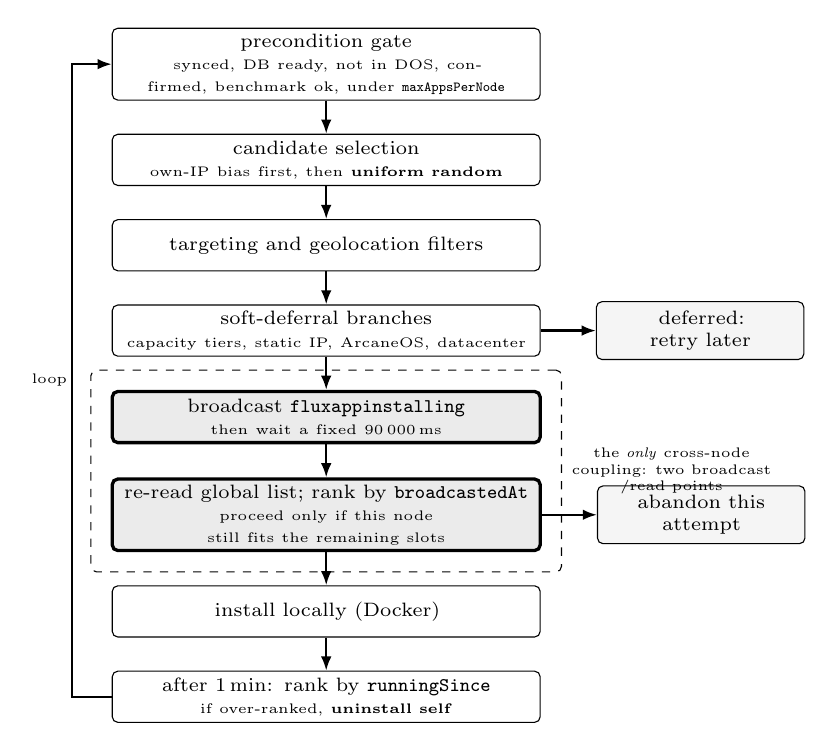
\begin{tikzpicture}[
  font=\scriptsize, node distance=4.2mm,
  stp/.style={draw, rounded corners=2pt, align=center, text width=52mm, minimum height=6.5mm,
              inner ysep=2pt},
  cross/.style={stp, very thick, fill=black!8},
  outbox/.style={draw, rounded corners=2pt, align=center, text width=24mm, fill=black!4,
              minimum height=6mm, font=\scriptsize},
  arr/.style={-{Latex[length=1.8mm]}, thick},
  lbl/.style={font=\tiny, inner sep=1.5pt, align=left},
]
  \node[stp]                     (gate)  {precondition gate\\{\tiny synced, DB ready, not in DOS, confirmed, benchmark ok, under \texttt{maxAppsPerNode}}};
  \node[stp, below=of gate]      (pick)  {candidate selection\\{\tiny own-IP bias first, then \textbf{uniform random}}};
  \node[stp, below=of pick]      (filt)  {targeting and geolocation filters};
  \node[stp, below=of filt]      (defer) {soft-deferral branches\\{\tiny capacity tiers, static IP, ArcaneOS, datacenter}};
  \node[cross, below=of defer]   (bcast) {broadcast \texttt{fluxappinstalling}\\{\tiny then wait a fixed \SI{90000}{\milli\second}}};
  \node[cross, below=of bcast]   (rank)  {re-read global list; rank by \texttt{broadcastedAt}\\{\tiny proceed only if this node still fits the remaining slots}};
  \node[stp, below=of rank]      (inst)  {install locally (Docker)};
  \node[stp, below=of inst]      (self)  {after \SI{1}{\minute}: rank by \texttt{runningSince}\\{\tiny if over-ranked, \textbf{uninstall self}}};

  \foreach \x/\y in {gate/pick, pick/filt, filt/defer, defer/bcast, bcast/rank, rank/inst, inst/self}
    \draw[arr] (\x) -- (\y);

  \node[outbox, right=7mm of defer] (dfr) {deferred: retry later};
  \node[outbox, right=7mm of rank]  (aba) {abandon this attempt};
  \draw[arr] (defer) -- (dfr);
  \draw[arr] (rank)  -- (aba);

  \draw[arr] (self.west) -- ++(-5mm,0) |- node[lbl, left, pos=0.25] {loop} (gate.west);

  \node[draw, dashed, rounded corners=2pt, inner sep=2.5mm, fit=(bcast)(rank),
        label={[font=\tiny, align=center]right:{the \emph{only} cross-node\\coupling: two broadcast\\/read points}}] {};
\end{tikzpicture}
\caption{Placement flow for one node's attempt at one application. The loop is private to a single
node: every step is a local decision, and the only coupling to other nodes is the broadcast/read pair
shown dashed. Conflicts are resolved by earliest-broadcast-wins, not by election or arbitration —
there is no scheduler in this picture, and that is the point \shipped
\srccode{flux/\allowbreak{}ZelBack/\allowbreak{}src/\allowbreak{}services/\allowbreak{}appLifecycle/\allowbreak{}appSpawner.js}{77--787}.}
\label{fig:placement-flow}
\end{figure}

\subsection{The reconciler: a single, level-based actuator}
\label{sec:fluxos-reconciler}

Once a container exists, everything that starts or stops it goes through one component,
documented in its own source as "the single, level-based actuator for app containers"
\srcdoc{flux/ZelBack/src/services/appMonitoring/appReconciler.js:20-27}. Every trigger — a Docker
\texttt{die} event, a stream reconnect, an hourly tick, boot, a post-install callback, or a
master/slave (syncthing) decision — only \emph{enqueues} a component identifier;
\texttt{reconcile()} is the only function that calls \texttt{appDockerStart}\slash\texttt{appDockerStop}
\srccode{flux/\allowbreak{}ZelBack/\allowbreak{}src/\allowbreak{}services/\allowbreak{}appMonitoring/\allowbreak{}appReconciler.js}{20--27}.

Desired state is resolved from four inputs, in strict priority order, highest wins
\srcdoc{flux/ZelBack/src/services/appMonitoring/appReconciler.js:29-45}:
\begin{enumerate}
\item \texttt{operator\allowbreak{}Stopped} — durable, persisted in \texttt{apps\allowbreak{}Runtime\allowbreak{}State}. The source calls
  this "user lock, wins over all."
\item \texttt{controller\allowbreak{}Desired} — in-memory only, re-derived every cycle by the master/slave and
  syncthing deciders. The source states why it is \emph{not} persisted: "a stale election after a
  reboot must not act."
\item \texttt{dataDesired} — an in-memory "clear" flag requesting an app-data wipe before the next
  run, also not persisted, for the same class of reason: "a stale wipe intent surviving a restart
  could delete the only good copy."
\item Restart policy and the last exit code, as the residual default.
\end{enumerate}
The syncthing/master-slave decider that feeds \texttt{controller\allowbreak{}Desired} is a second, large state
machine (\texttt{syncthingFolderStateMachine.\allowbreak{}js}, \texttt{syncthing\allowbreak{}Monitor.\allowbreak{}js}) that this evidence
pass did not read in depth; only its output channel into the reconciler is characterized here
\srcinferred.

Concurrency is single-flight per component identifier: an \texttt{inFlight} set prevents two
reconciles of the same component from running at once, and a \texttt{dirty} set forces one more
pass if the identifier was re-enqueued while a reconcile was already running
\srccode{flux/\allowbreak{}ZelBack/\allowbreak{}src/\allowbreak{}services/\allowbreak{}appMonitoring/\allowbreak{}appReconciler.js}{51--52}. A boot drain gate (an
\texttt{AsyncGate}) holds all boot-time triggers in \texttt{bootPending} until every boot-held
component has completed \emph{one} reconcile pass — not until all are running — capped at
\texttt{BOOT\_DRAIN\_SETTLE\_CAP\_MS} = 2\,min, so a single wedged reconcile can never indefinitely
suppress the node's own network-presence broadcast
\srccode{flux/\allowbreak{}ZelBack/\allowbreak{}src/\allowbreak{}services/\allowbreak{}appMonitoring/\allowbreak{}appReconciler.js}{55--64}. A container found
detached from its own Docker network — a stale libnetwork endpoint that a plain start cannot repair
— is force-removed and recreated rather than merely restarted
\srcdoc{flux/ZelBack/src/services/appMonitoring/appReconciler.js:24-26}. Crash recovery follows a
fixed backoff ladder, \texttt{crash\allowbreak{}Backoff\allowbreak{}Delays\allowbreak{}Ms} = [0, 30{,}000, 300{,}000, 900{,}000,
1{,}800{,}000]\,ms (0\,s, 30\,s, 5\,min, 15\,min, 30\,min), reset to the first rung after
\texttt{crash\allowbreak{}Backoff\allowbreak{}Stable\allowbreak{}Run\allowbreak{}Ms} = 600{,}000\,ms (10\,min) of stable running
\srccode{flux/\allowbreak{}ZelBack/\allowbreak{}config/\allowbreak{}default.js}{130--131}.

\subsection{Soft versus hard redeploy}
\label{sec:fluxos-redeploy}

Redeploy, removal, and installation are mutually exclusive with each other through four boolean
globals — \texttt{globalState.\allowbreak{}removalInProgress}, \texttt{installation\allowbreak{}In\allowbreak{}Progress},
\texttt{soft\allowbreak{}Redeploy\allowbreak{}In\allowbreak{}Progress}, \texttt{hard\allowbreak{}Redeploy\allowbreak{}In\allowbreak{}Progress} — checked at entry. If any is
already set, the call returns a warning and does nothing; it does not queue itself and does not
retry \srccode{flux/\allowbreak{}ZelBack/\allowbreak{}src/\allowbreak{}services/\allowbreak{}appLifecycle/\allowbreak{}advancedWorkflows.js}{1245--1281,1355--1383}.

\begin{table}[H]
\centering
\caption{Soft versus hard redeploy.}
\begin{tabular}{l l l}
\toprule
& Soft redeploy & Hard redeploy \\
\midrule
Teardown & \texttt{soft\allowbreak{}Remove\allowbreak{}App\allowbreak{}Locally}: stops/removes the container,
  \textbf{keeps} the app volume/data & \texttt{appUninstaller.\allowbreak{}removeAppLocally(force=false)}: full
  teardown, \textbf{drops} volumes \\
Wait & \texttt{config.\allowbreak{}fluxapps.\allowbreak{}redeploy.\allowbreak{}delay} = 30\,s & 30\,s (same constant) \\
Rebuild & \texttt{check\allowbreak{}App\allowbreak{}Requirements} then
  \texttt{soft\allowbreak{}Register\allowbreak{}App\allowbreak{}Locally} (recreate container against existing data) &
  \texttt{check\allowbreak{}App\allowbreak{}Requirements} then \texttt{appInstaller.registerAppLocally(...,\allowbreak{}
  sendRemovalMessage=true)} (full fresh install) \\
\bottomrule
\end{tabular}
\srccode{flux/\allowbreak{}ZelBack/\allowbreak{}src/\allowbreak{}services/\allowbreak{}appLifecycle/\allowbreak{}advancedWorkflows.js}{1313--1330,1394--1420}
\end{table}

\textbf{Automatic escalation.} For \specv{8}-and-later apps, if the installed component structure
differs from the target specification — component count or composition changed —
\texttt{softRedeploy} escalates itself to \texttt{hardRedeploy} instead of proceeding, "for
component structure safety" \srccode{flux/\allowbreak{}ZelBack/\allowbreak{}src/\allowbreak{}services/\allowbreak{}appLifecycle/\allowbreak{}advancedWorkflows.js}{1281--1305}.
If either path fails, the app is force-removed
(\texttt{removeAppLocally(.\allowbreak{}.\allowbreak{}.\allowbreak{}, force=true, sendMessage=true)}) as cleanup
\srccode{flux/\allowbreak{}ZelBack/\allowbreak{}src/\allowbreak{}services/\allowbreak{}appLifecycle/\allowbreak{}advancedWorkflows.js}{1332--1341,1422--1427}. Both
paths stream progress back over the original HTTP response (\texttt{res.write}) when one is
available: this is a synchronous, long-running HTTP call, not a job queue a client polls.

\subsection{The P2P layer}
\label{sec:fluxos-p2p}

\subsubsection{Wire format, dispatch, dedup}
Every \FluxOS-to-\FluxOS message is JSON over WebSocket, wrapped in a signed envelope
\texttt{\{version:\,\allowbreak{}1,\allowbreak{} timestamp,\allowbreak{} pubKey,\allowbreak{} signature (over version+message+timestamp),\allowbreak{} data\}}
\srccode{flux/\allowbreak{}ZelBack/\allowbreak{}src/\allowbreak{}services/\allowbreak{}utils/\allowbreak{}fluxBroadcastHelper.js}{11--26}. Observed
\texttt{data.type} values: \texttt{zelappregister}\slash\texttt{fluxappregister},
\texttt{zelappupdate}\slash\texttt{fluxappupdate}, \texttt{fluxapprequest} (a v1 single-hash form and a
v2 form batching up to 500 hashes), \texttt{fluxapprunning}, \texttt{fluxipchanged},
\texttt{fluxappremoved}, \texttt{fluxappinstalling}, \texttt{fluxappinstallingerror},
\texttt{fluxnodesigterm}, and four sync-round types
(\texttt{fluxapptempsync}, \texttt{fluxapprunningsync}, \texttt{fluxappinstallingsync},
\texttt{fluxappinstallingerrorssync}) \srccode{flux/\allowbreak{}ZelBack/\allowbreak{}src/\allowbreak{}services/\allowbreak{}fluxCommunication.js}{585--602,644--660}
\srccode{flux/\allowbreak{}ZelBack/\allowbreak{}src/\allowbreak{}services/\allowbreak{}fluxCommunicationMessagesSender.js}{53--74}. A separate raw,
non-JSON channel — \texttt{message\allowbreak{}Hash\allowbreak{}Present} (a 40-char hex hash) and
\texttt{request\allowbreak{}Message\allowbreak{}Hash} — bypasses the signed envelope entirely, because it only ever carries a
hash and never application data \srccode{flux/\allowbreak{}ZelBack/\allowbreak{}src/\allowbreak{}services/\allowbreak{}fluxCommunication.js}{511--536}.

Inbound dispatch (\texttt{dispatch\allowbreak{}Flux\allowbreak{}Message}) runs, per message: raw hash-gossip frames first,
handled and returned immediately, no signature check
\srccode{flux/\allowbreak{}ZelBack/\allowbreak{}src/\allowbreak{}services/\allowbreak{}fluxCommunication.js}{511--536}; a malformed envelope closes the
connection \srccode{flux/\allowbreak{}ZelBack/\allowbreak{}src/\allowbreak{}services/\allowbreak{}fluxCommunication.js}{538--546}; deduplication after
a random 1--75\,ms jitter delay against an in-memory \texttt{messageCache} keyed on
\texttt{hash(data)} — a seen hash is silently dropped
\srccode{flux/\allowbreak{}ZelBack/\allowbreak{}src/\allowbreak{}services/\allowbreak{}fluxCommunication.js}{549--554} (the exact TTL/eviction policy
of this cache was not traced to its definition in the evidence available \srcinferred); a blocklist
check against \texttt{wsPeerCache}
\srccode{flux/\allowbreak{}ZelBack/\allowbreak{}src/\allowbreak{}services/\allowbreak{}fluxCommunication.js}{556--563}; then signature/timestamp
verification, yielding \texttt{OK}, \texttt{NODE\_NOT\_FOUND} (originator not in the deterministic
node list — dropped without penalizing the relaying peer, "the relay peer is not at fault"), or a
bad-signature/malformed result, which is tracked per-peer in a rolling 10-minute window and closes
the connection at 5 or more bad messages in that window (the timestamp array is capped at 20
entries, truncated to the last 10, bounding memory from an adversarial peer)
\srccode{flux/\allowbreak{}ZelBack/\allowbreak{}src/\allowbreak{}services/\allowbreak{}fluxCommunication.js}{592--618}. A valid, fresh message is
dispatched by type via \texttt{setImmediate} — deferred one tick, not otherwise queued or
rate-limited per type \srccode{flux/\allowbreak{}ZelBack/\allowbreak{}src/\allowbreak{}services/\allowbreak{}fluxCommunication.js}{604--618}; a stale
but otherwise valid message gets a NAK rather than a silent drop
\srccode{flux/\allowbreak{}ZelBack/\allowbreak{}src/\allowbreak{}services/\allowbreak{}fluxCommunication.js}{601}. Four message types
(\texttt{fluxapprunning}, \texttt{fluxipchanged}, \texttt{fluxappremoved}, \texttt{fluxnodesigterm}) use a 240{,}000\,ms
(4\,min) freshness window \srccode{flux/\allowbreak{}ZelBack/\allowbreak{}src/\allowbreak{}services/\allowbreak{}fluxCommunication.js}{317,405,437,465}.

\subsubsection{Rebroadcast and convergence}
Rebroadcast follows one of two mutually exclusive strategies, selected by comparing daemon height
to \texttt{messages\allowbreak{}Broadcast\allowbreak{}Refactor\allowbreak{}Start} = 1{,}751{,}250 ("expected block at 13th October 2024"
per the code's own comment \srcdoc{flux/ZelBack/config/default.js:124}): below it,
\texttt{fluxCommunicationMessagesSender.\allowbreak{}relay(.\allowbreak{}.\allowbreak{}.\allowbreak{})} flood-fills the full signed message to every
other peer; at or above it, only the 40-character hash is gossiped
(\texttt{peerManager.\allowbreak{}broadcastHash}), and a receiver that lacks the body pulls it on demand via
\texttt{request\allowbreak{}Message\allowbreak{}Hash} \srccode{flux/\allowbreak{}ZelBack/\allowbreak{}src/\allowbreak{}services/\allowbreak{}fluxCommunication.js}{407--412,431--436,486--491}.
This is a live protocol transition keyed on chain height, not a node-local configuration flag. A
\texttt{fluxnodesigterm} broadcast extends the affected apps' \texttt{expireAt} in
\texttt{zelappslocation} to \texttt{broadcastedAt} $+$ \texttt{SIGTERM\_EXPIRY\_MS}
(420{,}000\,ms, 7\,min) rather than letting the location expire immediately
\srccode{flux/\allowbreak{}ZelBack/\allowbreak{}src/\allowbreak{}services/\allowbreak{}fluxCommunication.js}{472--478}
\srccode{flux/\allowbreak{}ZelBack/\allowbreak{}src/\allowbreak{}services/\allowbreak{}utils/\allowbreak{}appConstants.js}{86}. Beyond continuous gossip, a
periodic hash-sync protocol runs with its own bounded parameters — up to
\texttt{hash\allowbreak{}Sync\allowbreak{}Max\allowbreak{}Rounds} = 4 rounds, \texttt{hash\allowbreak{}Sync\allowbreak{}Peers\allowbreak{}Per\allowbreak{}Round} = 3,
\texttt{hash\allowbreak{}Sync\allowbreak{}Ephemeral\allowbreak{}Peers} = 5, \texttt{hash\allowbreak{}Sync\allowbreak{}Max\allowbreak{}Retries} = 3 at
\texttt{hash\allowbreak{}Sync\allowbreak{}Retry\allowbreak{}Ms} = 300{,}000\,ms, with a \texttt{hash\allowbreak{}Sync\allowbreak{}Settle\allowbreak{}Ms} = 4{,}000\,ms settle
window \srccode{flux/\allowbreak{}ZelBack/\allowbreak{}config/\allowbreak{}default.js}{355--363}; the exact message sequence of one full
round (who is asked, in what order, what happens on a partial response) was not traced beyond these
constants \srcinferred.

\textbf{This is gossip convergence, not consensus.} Global application state — which node is
running, installing, or has removed which application — lives in \texttt{globalzelapps}, is
propagated exclusively by the dedup/rebroadcast/hash-sync mechanism above, TTL-expires by the
constants in Table~\ref{tab:lifecycle-timing}, and is not committed to any block, checked against any
quorum, or given any finality. Two nodes with a partitioned or lagging gossip view can disagree
about the current state of an application for as long as the partition lasts; nothing above the
mesh corrects that disagreement faster than the mesh itself re-converges.

\subsubsection{Peer topology and liveness}
\texttt{Flux\allowbreak{}Peer\allowbreak{}Manager} is a single in-memory registry of inbound and outbound sockets, ephemeral
sync peers, a reconnect queue tracking per-peer attempts, an unstable-node tracker, IP-group/unique-IP
counters, and a bounded circular history buffer of peer lifecycle events
\srccode{flux/\allowbreak{}ZelBack/\allowbreak{}src/\allowbreak{}services/\allowbreak{}utils/\allowbreak{}FluxPeerManager.js}{31--77}. Inbound admission is capped at
the larger of \texttt{maxPeers} = $4\times$\texttt{minIncoming} and \texttt{max\allowbreak{}Number\allowbreak{}Of\allowbreak{}Connections}, which is normally
$9\times$\texttt{minIncoming} but scales down when \texttt{number\allowbreak{}Of\allowbreak{}Flux\allowbreak{}Nodes}/160 falls below that
figure, so small networks get a proportionally smaller inbound cap rather than a flat one, floored at \texttt{maxPeers}
\srccode{flux/\allowbreak{}ZelBack/\allowbreak{}src/\allowbreak{}services/\allowbreak{}utils/\allowbreak{}FluxPeerManager.js}{839--847}. Reconnect backoff follows
[120{,}000, 300{,}000, 600{,}000, 900{,}000]\,ms (2/5/10/15\,min)
\srccode{flux/\allowbreak{}ZelBack/\allowbreak{}src/\allowbreak{}services/\allowbreak{}utils/\allowbreak{}FluxPeerManager.js}{32}. Liveness is a WebSocket ping
every \texttt{ws\allowbreak{}Ping\allowbreak{}Interval\allowbreak{}Ms} = 15{,}000\,ms; a peer that misses 3 consecutive pongs
(\texttt{ws\allowbreak{}Max\allowbreak{}Missed\allowbreak{}Pongs}) is force-terminated
\srccode{flux/\allowbreak{}ZelBack/\allowbreak{}config/\allowbreak{}default.js}{18--19}
\srccode{flux/\allowbreak{}ZelBack/\allowbreak{}src/\allowbreak{}services/\allowbreak{}utils/\allowbreak{}FluxPeerSocket.js}{86--145,209--212,298}. Placement itself
is gated on this liveness signal: the spawner runs only above an \texttt{app\allowbreak{}Sync\allowbreak{}Peer\allowbreak{}Threshold} of
12 live peers and pauses below an \texttt{app\allowbreak{}Sync\allowbreak{}Degraded\allowbreak{}Threshold} of 4
\srccode{flux/\allowbreak{}ZelBack/\allowbreak{}config/\allowbreak{}default.js}{268--269}
\srccode{flux/\allowbreak{}ZelBack/\allowbreak{}src/\allowbreak{}services/\allowbreak{}appLifecycle/\allowbreak{}appSpawner.js}{38--52}.

\subsection{Resource accounting}
\label{sec:fluxos-resources}

\begin{table}[H]
\centering
\caption{Per-tier resource allowances (total / available to applications).}
\begin{tabular}{l l l l l}
\toprule
Tier & CPU (units of 0.1 core) & RAM (MB) & HDD (GB) & Collateral, current / legacy (\flux) \\
\midrule
Cumulus ($\tC$) & 40 / 30 & 7{,}000 / 5{,}000 & 220 / 180 & 1{,}000 / 10{,}000 \\
Nimbus ($\tN$) & 80 / 70 & 30{,}000 / 28{,}000 & 440 / 400 & 12{,}500 / 25{,}000 \\
Stratus ($\tS$) & 160 / 150 & 61{,}000 / 59{,}000 & 880 / 840 & 40{,}000 / 100{,}000 \\
\bottomrule
\end{tabular}
\srccode{flux/\allowbreak{}ZelBack/\allowbreak{}config/\allowbreak{}default.js}{380--403}
\end{table}

Resources locked by the host system, subtracted before any application allocation:
\texttt{cpu}: 10 (one core, in units of 0.1 core), \texttt{ram}: 2{,}000\,MB, \texttt{hdd}: 60\,GB,
\texttt{extrahdd}: 20\,GB \srccode{flux/\allowbreak{}ZelBack/\allowbreak{}config/\allowbreak{}default.js}{375--378}, with a further 0.95
usable-disk multiplier \srccode{flux/\allowbreak{}ZelBack/\allowbreak{}src/\allowbreak{}services/\allowbreak{}appRequirements/\allowbreak{}hwRequirements.js}{385}.
\texttt{hwRequirements.\allowbreak{}checkAppHWRequirements} enforces, per component:
\begin{multline*}
\text{usable HDD} = 0.95\cdot\text{total HDD} - 60 - 20, \\
\text{reject if } \text{app HDD} > \text{usable HDD} - \text{HDD locked by other apps};
\end{multline*}
\begin{multline*}
\text{usable CPU (}\times 10\text{)} = 10\cdot\text{cores} - 10, \\
\text{reject if } 10\cdot\text{app CPU} > \text{usable CPU} - 10\cdot\text{CPU locked by other apps};
\end{multline*}
\begin{multline*}
\text{usable RAM} = \text{total RAM} - 2{,}000, \\
\text{reject if app RAM} > \text{usable RAM} - \text{RAM locked by other apps}
\end{multline*}
\srccode{flux/\allowbreak{}ZelBack/\allowbreak{}src/\allowbreak{}services/\allowbreak{}appRequirements/\allowbreak{}hwRequirements.js}{370--408}. A separate,
enterprise-only check additionally rejects an install that would leave 4 or fewer free vCores after
it (\texttt{free\allowbreak{}Cores\allowbreak{}After\allowbreak{}Install} = cores $-$ 1 system-reserved core $-$ locked cores $-$ app
cores), reserved so the CFS CPU-burst feature always has spare capacity to draw on
\srccode{flux/\allowbreak{}ZelBack/\allowbreak{}src/\allowbreak{}services/\allowbreak{}appRequirements/\allowbreak{}hwRequirements.js}{411--437}. That burst feature
is enabled by default (\texttt{cpuBurst.\allowbreak{}enabled: true}, CFS period \texttt{periodUs} = 100{,}000
(100\,ms), 1 reserved core) \srccode{flux/\allowbreak{}ZelBack/\allowbreak{}config/\allowbreak{}default.js}{440--453}, with the per-host
caveat, stated in the source itself, that "multiple burstable apps on the same host can
collectively oversubscribe during simultaneous spikes"
\srcdoc{flux/ZelBack/config/default.js:441-449}.

\subsection{Pricing}
\label{sec:fluxos-pricing}

Price is computed from a per-component resource vector $\resvec$, the requested instance count
$\ninst$, and the requested duration $\dur$ (in blocks, against $\blockslasting$), evaluated at the
transaction's block height $\hgt$ against a height-scheduled price table
(\texttt{config.\allowbreak{}fluxapps.\allowbreak{}price[]}, overridable by \texttt{chainmessages} of type \texttt{p} posted
on-chain by the Foundation multisig) \srccode{flux/\allowbreak{}ZelBack/\allowbreak{}src/\allowbreak{}services/\allowbreak{}utils/\allowbreak{}chainUtilities.js}{9--52}.
Concretely, for a \specv{4}-or-later (composed) app, \texttt{cpuPrice} $= \sum$(CPU units)
$\times\,\text{table.cpu}\times 10$; \texttt{ramPrice} $=\sum$(RAM units)
$\times\,\text{table.ram}/100$; \texttt{hddPrice} $=\sum$(HDD units) $\times\,\text{table.hdd}$;
plus \texttt{table.scope} if the app declares \texttt{nodes} or is \texttt{enterprise}, plus
\texttt{table.staticip} if it declares \texttt{staticip}, plus \texttt{table.port} per enterprise
port; that sum is quoted per three instances --- divided by three, ceiled to two decimals, and, from
height \num{1890000}, scaled by the requested instance count $\ninst$, with a floor of $0.50$ per
additional instance for the cheapest specifications
\srccode{flux/\allowbreak{}ZelBack/\allowbreak{}src/\allowbreak{}services/\allowbreak{}utils/\allowbreak{}appUtilities.js}{89--134}. The registration price is then
scaled by $\dur/\text{defaultExpire}$, where \texttt{defaultExpire} is $\blockslasting$ or
$4\times\blockslasting$ post-\PoN fork, re-ceiled, and only then floored at \texttt{minPrice}
\srccode{flux/\allowbreak{}ZelBack/\allowbreak{}src/\allowbreak{}services/\allowbreak{}appMessaging/\allowbreak{}messageVerifier.js}{733--743}; an update is priced
at 90\% of the fresh price minus a further discount proportional to the unused life of the prior
spec, floored again at \texttt{minPrice} \srccode{flux/\allowbreak{}ZelBack/\allowbreak{}src/\allowbreak{}services/\allowbreak{}appMessaging/\allowbreak{}messageVerifier.js}{801--816}.
\S16 gives the full pricing mechanics and treats the credits/renewal layer built on top of them;
here it is enough to record the one finding that changes what a payer can rely on:
\textbf{an underpaid registration or update is silently dropped, with only a server-side log
warning and no signal of any kind returned to the payer}
(\S\ref{sec:fluxos-lifecycle}; \srccode{flux/\allowbreak{}ZelBack/\allowbreak{}src/\allowbreak{}services/\allowbreak{}appMessaging/\allowbreak{}messageVerifier.js}{735--763,797--828}).
\S16 takes up what a correct failure signal would require.

\subsection{Moderation, as it exists today}
\label{sec:fluxos-moderation}

Docker image compliance is enforced against a GitHub-hosted list, not an on-chain or
network-quorum one: \texttt{get\allowbreak{}Blocked\allowbreak{}Repositores()} fetches
\texttt{helpers/\allowbreak{}blockedrepositories.\allowbreak{}json} from \texttt{raw.\allowbreak{}githubusercontent.\allowbreak{}com/\allowbreak{}RunOnFlux/\allowbreak{}flux},
cached in \texttt{fluxCaching.\allowbreak{}blockedRepositoriesCache}
\srccode{flux/\allowbreak{}ZelBack/\allowbreak{}src/\allowbreak{}services/\allowbreak{}appSecurity/\allowbreak{}imageManager.js}{179--195}; a parallel
\texttt{vettedrepositories.\allowbreak{}json} lets listed apps bypass user-defined blocked ports and repositories
\srccode{flux/\allowbreak{}ZelBack/\allowbreak{}src/\allowbreak{}services/\allowbreak{}appSecurity/\allowbreak{}imageManager.js}{202--236,395--410}.
\texttt{check\allowbreak{}Applications\allowbreak{}Compliance} runs every \texttt{image\allowbreak{}Compliance\allowbreak{}Interval\allowbreak{}Ms} =
3{,}600{,}000\,ms (1\,h), removing any locally installed app that matches the blocklist and waiting
3\,min between removals "so we don't have more removals at the same time"
\srccode{flux/\allowbreak{}ZelBack/\allowbreak{}src/\allowbreak{}services/\allowbreak{}serviceManager.js}{529--531}
\srccode{flux/\allowbreak{}ZelBack/\allowbreak{}config/\allowbreak{}default.js}{319}
\srccode{flux/\allowbreak{}ZelBack/\allowbreak{}src/\allowbreak{}services/\allowbreak{}appSecurity/\allowbreak{}imageManager.js}{644--676}. The equivalent
GitHub-sourced enterprise node/owner map resyncs every 6\,h with fetch failure explicitly swallowed
by a \texttt{.catch} handler, proceeding on the last-cached value
\srccode{flux/\allowbreak{}ZelBack/\allowbreak{}src/\allowbreak{}services/\allowbreak{}serviceManager.js}{130--136}; the evidence gathered for this
paper did not separately trace a distinct failure-handling code path for the blocklist fetch itself
beyond its cache, but the two fetches share the same GitHub-hosted, silently-cached design.
\S23 analyzes what this means for censorship-resistance and for the roadmap's stated network-quorum
vision; this section states the mechanism and defers the analysis.

\subsection{Trust and failure model}
\label{sec:fluxos-trust}

\begin{enumerate}
\item \textbf{Placement convergence assumes peer honesty.} Instance-count convergence depends
  entirely on nodes honestly reporting and honoring \texttt{broadcastedAt} rank; nothing in the
  paths read re-verifies it against the signed envelope's own timestamp for this message type
  \srcinferred (\S\ref{sec:fluxos-placement}).
\item \textbf{Underpayment is swallowed, not rejected.} A registration or update that pays too
  little produces only a log warning; the payer receives no on-chain refund and no distinguishable
  failure signal \srccode{flux/\allowbreak{}ZelBack/\allowbreak{}src/\allowbreak{}services/\allowbreak{}appMessaging/\allowbreak{}messageVerifier.js}{735--763,797--828}.
\item \textbf{GitHub is the moderation trust root.} The image blocklist, vetted-repository list,
  and enterprise owner map are all fetched from one GitHub repository on a schedule, with fetch
  failure silently swallowed and the last-good value kept
  \srccode{flux/\allowbreak{}ZelBack/\allowbreak{}src/\allowbreak{}services/\allowbreak{}serviceManager.js}{130--136}; a GitHub outage or a compromise
  of that specific file is a single point of moderation trust for the whole network, not a
  network-quorum mechanism (\S\ref{sec:fluxos-moderation}).
\item \textbf{Boot is a flat-backoff infinite retry, not a circuit breaker.} Any uncaught exception
  in the boot function restarts it after a fixed 15{,}000\,ms with no retry cap and no escalation,
  so a persistently failing dependency retries forever rather than surfacing a fatal state
  \srccode{flux/\allowbreak{}ZelBack/\allowbreak{}src/\allowbreak{}services/\allowbreak{}serviceManager.js}{568--572}.
\item \textbf{Distributed enforcement trusts a synchronized local view.} The node-status monitor's
  network-wide eviction pass — which every confirmed node runs independently against every other
  node's claimed locations — trusts its own local copy of the deterministic node list; if that
  local view lags, it can evict still-valid locations or fail to evict dead ones \srcinferred.
\item \textbf{Self-correction can amplify churn under partition.} Because every node independently
  re-derives whether an application is over-replicated and removes itself on that basis, a
  partition that produces disjoint \texttt{runningSince} orderings can cause more nodes to remove
  an application than intended, or none, until gossip re-converges; there is no distributed lock
  (\S\ref{sec:fluxos-placement}, remark above).
\item \textbf{\texttt{admin} is a local file, not a bound credential.} \texttt{admin} privilege is
  granted to whoever controls \texttt{userconfig.\allowbreak{}initial.\allowbreak{}zelid} on that specific node's disk; there
  is no additional hardware or HSM binding checked at this privilege level
  \srccode{flux/\allowbreak{}ZelBack/\allowbreak{}src/\allowbreak{}services/\allowbreak{}verificationHelperUtils.js}{19--46}.
\end{enumerate}

%% Drain this section's float queue before the next begins.
\FloatBarrier

\section{FluxOS application specification v9}
\label{sec:appspec-v9}

Every application that runs on \Flux is described by a small, owner-signed JSON document: a
container image, how much CPU, memory and disk it needs, how many copies to run, and for how long.
Because \FluxOS has no central scheduler and instead relies on every node independently deciding
what to run (\S9), that document is closer to a consensus artifact than to an ordinary
application-programming detail — every node on the network must parse and validate it the same
way, which is why changing its shape is slow and height-gated, exactly like a price table. This
section describes the specification version currently enforced on the network, and a substantial,
actively-developed redesign that is not enforced anywhere yet. This paper calls the specification
version \emph{v9} throughout, written in full here and as \specv{9} from this point on; it is
unrelated to \daemonversion, the version number of the consensus daemon \fluxd, which is
maintained independently and is never the referent of ``v9'' in this document
\srcintent{design intake}. The reason this section exists is structural, not archival: three fields
\specv{9} adds — \texttt{paymentMemo}, \texttt{referralCode} and \texttt{machineType} — are the
substrate that \PNR (\S7), the referral program, and the VPS/datacenter tier (\S11) are each stated
to depend on, and as of this writing none of the three has any consumer code anywhere in \FluxOS.

\subsection{Version gating as deployed}

\FluxOS accepts an incoming specification $s$ at chain height \hgt only if its declared version does
not exceed the maximum version enforced at that height, its top-level and per-component fields are
drawn from that version's whitelist, and it otherwise satisfies that version's own validity rules:
$$
\mathrm{Accept}(s,\hgt) \;\equiv\; v(s) \le V(\hgt) \;\wedge\; \mathrm{Fields}(s) \subseteq
\mathcal{F}_{v(s)} \;\wedge\; \mathrm{Valid}_{v(s)}(s),
$$
with $V(\hgt)$ the highest specification version whose enforcement height has been reached. This is
the same height-scheduling mechanism the network uses for price-table changes, applied to the
specification schema itself: \texttt{verify\allowbreak{}App\allowbreak{}Specifications} runs type correctness, then
per-version restriction checks, then the enforcement-height gate, then object-key correctness
against a per-version field whitelist, in that fixed order, before anything is broadcast \shipped\ \srccode{flux/\allowbreak{}ZelBack/\allowbreak{}src/\allowbreak{}services/\allowbreak{}appRequirements/\allowbreak{}appValidator.js}{1243-1400}.

The enforcement-height table, as configured today, is:

\begin{table}[H]
\centering
\small
\begin{tabular}{@{}llp{6.5cm}@{}}
\toprule
Version & Enforcement height & Notes \\
\midrule
1 & 0 & no longer accepted for registration or update via the API \\
2 & 0 & \\
3 & 983{,}000 & \\
4 & 1{,}004{,}000 & composition (\texttt{compose} array) \\
5 & 1{,}142{,}000 & \texttt{contacts}, \texttt{geolocation} \\
6 & 1{,}300{,}000 & \texttt{expire}, price change \\
7 & 1{,}420{,}000 (mainnet) / 1{,}390{,}000 (dev) & \texttt{nodes} targeting, \texttt{secrets}, \texttt{staticip} \\
8 & \textbf{1{,}932{,}380} (mainnet) / \textbf{1{,}921{,}500} (dev) & enterprise / ArcaneOS apps \\
\bottomrule
\end{tabular}
\caption{Specification-version enforcement heights as shipped in \FluxOS. There is no row for
version 9: no enforcement height for it exists in the shipped configuration or the live pricing
endpoint (below).}
\end{table}

\shipped\ \srccode{flux/\allowbreak{}ZelBack/\allowbreak{}config/\allowbreak{}default.js}{231-240}, cross-checked against the live public
pricing endpoint, which returns the identical mainnet heights through version 8 and carries no key
for version 9 at all \srcmeasured{api.runonflux.io/\allowbreak{}apps/\allowbreak{}deploymentinformation}{2026-09-03}.
\specv{8}'s enforcement height is \textbf{1{,}932{,}380} on mainnet and \textbf{1{,}921{,}500} in the
development network \shipped\ \srccode{flux/\allowbreak{}ZelBack/\allowbreak{}config/\allowbreak{}default.js}{231-240}. Above that height, a
specification whose top-level keys are anything other than \texttt{version,\allowbreak{} name,\allowbreak{} description,\allowbreak{}
owner,\allowbreak{} compose,\allowbreak{} instances,\allowbreak{} contacts,\allowbreak{} geolocation,\allowbreak{} expire,\allowbreak{} nodes,\allowbreak{} staticip,\allowbreak{} datacenter,\allowbreak{} enterprise}
is rejected outright \shipped\ \srccode{flux/\allowbreak{}ZelBack/\allowbreak{}src/\allowbreak{}services/\allowbreak{}appRequirements/\allowbreak{}appValidator.js}{1063-1067}.

\inprogress\ The organisation's own working checkout additionally carries a single, unpublished
commit that begins to vendor a copy of the RFC-0 schema (\S\ref{sec:two-artifacts}) behind a feature flag
rather than a height: registering or updating a \texttt{version: 9} specification is rejected
before schema validation ever runs unless \texttt{config.\allowbreak{}fluxapps.\allowbreak{}acceptV9} is \texttt{true}, and
that flag defaults to \texttt{false} with no caller anywhere in the codebase that sets it
\srcbranch{RunOnFlux/\allowbreak{}flux}{feat/appspec-v9}{ZelBack/src/services/appDatabase/registryManager.js:1766-1769}.\footnote{%
This sits on a working checkout of the organisation repository that had not been pushed to
\texttt{RunOnFlux/flux}'s public remote at the time of writing, and it is a much smaller and
separate effort from the contributor fork discussed in \S\ref{sec:appspec-v9-scale}. It is cited
here as an unpublished working branch, not as a fetchable public artifact.} No node on the network
today enforces any rule for \texttt{version: 9} beyond ``reject it.''

\subsection{The migration baseline, measured}
\label{sec:migration-baseline}

The concrete cost of this gating scheme is visible in what is actually deployed. Of 1{,}195
applications registered on the network on 2026-09-03
\srcmeasured{api.runonflux.io/\allowbreak{}apps/\allowbreak{}globalappsspecifications}{2026-09-03}:

\begin{table}[H]
\centering
\begin{tabular}{@{}lrr@{}}
\toprule
Version & Applications & Share \\
\midrule
v8 & 873 & 73.1\% \\
v7 & 209 & 17.5\% \\
v6 & 70 & 5.9\% \\
v3 & 27 & 2.3\% \\
v4 & 11 & 0.9\% \\
v5 & 3 & 0.3\% \\
v2 & 2 & 0.2\% \\
\midrule
Total & 1{,}195 & 100\% \\
\bottomrule
\end{tabular}
\caption{Deployed-application count by specification version, ordered by share.}
\end{table}

\shipped\ \textbf{322 applications (26.9\%) are on a version older than \specv{8}.} Seven
specification versions — \specv{2} through \specv{8} — are live on the network simultaneously
\srcmeasured{api.runonflux.io/\allowbreak{}apps/\allowbreak{}globalappsspecifications}{2026-09-03}. The acceptance predicate
above has a ceiling ($v(s) \le V(\hgt)$) but no floor: nothing in it forces an already-running
application to move forward when a newer version becomes enforceable, and the measured coexistence
of seven versions is the direct, observable consequence. The network has not deprecated any
specification version to date; every version ever shipped is still validated, by every node, for as
long as an application on that version continues to exist. That is the real cost of
height-scheduled versioning with no deprecation mechanism, and it is the baseline against which
\specv{9}'s eventual migration has to be measured (\S\ref{sec:migration-mechanism}).

\subsection{What v9 changes}

\inprogress\ \specv{9} is defined, at present, only as a draft JSON Schema (RFC-0) in a standalone
repository \srccode{flux-spec/\allowbreak{}schema/\allowbreak{}v9.json}{1-350} — see \S\ref{sec:two-artifacts} for why that
draft and what \FluxOS actually consumes are not the same object. Table~\ref{tab:v9-changes}
summarises the delta against \specv{8}: four field renames, one removal, and five additions, each
against what depends on it and how far its implementation actually reaches.

\begin{table}[H]
\centering
\small
\begin{tabular}{@{}llp{3.6cm}p{4.4cm}@{}}
\toprule
Change & \specv{9} name (\specv{8} name) & Depends on & Implementation status \\
\midrule
Rename & \texttt{components} (\texttt{compose}) & --- & schema-level only; breaks every existing client, hence bundled with the other renames rather than dripped \\
Rename & \texttt{image} (\texttt{repotag}) & --- & schema-level only \\
Rename & \texttt{memory} (\texttt{ram}) & --- & schema-level only \\
Rename & \texttt{rootFsGb} (\texttt{hdd}) & --- & schema-level only \\
Removal & --- (\texttt{enterprise}; its envelope replacement named but not specified) & private/encrypted specifications & regression; see \S\ref{sec:envelope-regression} \\
Addition & \texttt{loadBalancing} & routing, health checks, backend TLS, connection draining & partially implemented: draining and per-app-CA TLS wired; config generation stays in \FDM (\S12) \\
Addition & \texttt{duration} & subscriptions and auto-renewal (\S16) & first-class in the schema; the fork's pricing engine reads the same concept off \texttt{spec.ttl}, and whether \texttt{duration} maps to it is unresolved (\S\ref{sec:app-interfaces}) \\
Addition & \texttt{paymentMemo} & \PNR (\S7) & \textbf{zero consumers in \FluxOS} \\
Addition & \texttt{referralCode} & referrals, preview environments & \textbf{zero consumers} \\
Addition & \texttt{machineType} & VPS/datacenter tier (\S11) & \textbf{zero consumers} \\
\bottomrule
\end{tabular}
\caption{\specv{8}$\to$\specv{9} field changes, their dependents, and implementation status.}
\label{tab:v9-changes}
\end{table}

Field shapes and required-field membership per \srccode{flux-spec/\allowbreak{}schema/\allowbreak{}v9.json}{40-46} (\texttt{components}),
\srccode{flux-spec/\allowbreak{}schema/\allowbreak{}v9.json}{47-61} (\texttt{loadBalancing}), \srccode{flux-spec/\allowbreak{}schema/\allowbreak{}v9.json}{62-82}
(\texttt{duration}, \texttt{paymentMemo}, \texttt{referralCode}, \texttt{machineType}), and
\srccode{flux-spec/\allowbreak{}schema/\allowbreak{}v9.json}{103-122} (\texttt{image}, \texttt{memory}, \texttt{rootFsGb}); the
removal of \texttt{enterprise}, with its envelope replacement deferred to a later revision, is stated in the draft's own README
\srcdoc{flux-spec/README.md:58-67,95-96}; the \texttt{paymentMemo}\slash\texttt{referralCode} dependency
mapping is drawn from the fork's own code comments (``basis for paying operators under PNR v2'',
``rewards paid as hosting credits'') \srcbranch{RunOnFlux/\allowbreak{}flux}{feat/appspec-v9}{ZelBack/src/services/appRequirements/appSpecV9.js}.

\subsection{The finding this section exists to deliver}
\label{sec:finding}

\inprogress\ Stated plainly and without spin: \texttt{paymentMemo}, \texttt{referralCode} and
\texttt{machineType} have \textbf{zero consumer code anywhere in \FluxOS} — no billing path, no
referral-reward path, no
capacity-tier scheduling path reads any of the three, confirmed by grepping every JavaScript file
under \texttt{ZelBack/} and \texttt{tests/} for all three field names
\srcbranch{MorningLightMountain713/\allowbreak{}flux}{feat/fluxos-v9}{(grep -rn "paymentMemo|referralCode|machineType" --include=*.js ZelBack tests)}.
Those are exactly the fields \PNR (\S7), the referral program, and the VPS tier (\S11) are stated to
depend on. The orchestration substrate of \specv{9} — placement, mesh identity, routing plumbing,
persistent storage, pricing — is built and tested (\S\ref{sec:appspec-v9-scale}); the economic
fields the roadmap's dependency chain actually rests on are declared in a schema and nothing more.
The dependency chain the roadmap draws between \specv{9} and \PNR, referrals and the VPS tier is
real at the level of the schema; it currently terminates in fields no code reads. \S\ref{sec:feasibility} returns to
this as one instance of a broader pattern in how far the remaining work actually reaches.

\subsection{The scale of the work, quantified}
\label{sec:appspec-v9-scale}

The overwhelming majority of \specv{9} engineering effort does not live in the organisation
repository. It lives on an individual contributor's fork\footnote{\texttt{MorningLightMountain713/\allowbreak{}flux},
branch \texttt{feat/fluxos-v9}, last pushed 2026-09-02 — an external fork of \texttt{RunOnFlux/flux},
not a branch of the organisation repository itself. Citations against it use
\textsf{[repo@branch:file:line]} notation for that reason, and none of them can be fetched from the
organisation's own remote.} that diffs 932 files against \texttt{upstream/\allowbreak{}master}, with
$+180{,}317/-49{,}561$ lines
\srcbranch{MorningLightMountain713/\allowbreak{}flux}{feat/fluxos-v9}{(git diff --stat upstream/master origin/feat/fluxos-v9)},
decomposing the old monolithic application-service layout into 23 focused service
packages, ten of them absent from \texttt{upstream/\allowbreak{}master} (\texttt{appMesh}, \texttt{appPlacement}, \texttt{pricing},
\texttt{quorumGrant}, and others)
\srcbranch{MorningLightMountain713/\allowbreak{}flux}{feat/fluxos-v9}{(find ZelBack/src -maxdepth 3 -type d)}.
This is \inprogress\ work, and it is substantial: 289 unit-test files containing 7{,}763 test cases
run on every push
\srcbranch{MorningLightMountain713/\allowbreak{}flux}{feat/fluxos-v9}{(find tests/unit -name *.test.js | wc -l = 289; grep count of it/test call sites in tests/unit = 7763)}
\srcbranch{MorningLightMountain713/\allowbreak{}flux}{feat/fluxos-v9}{.github/workflows/nodejs.yml:1-3,90-93},
alongside a from-scratch, 121-scenario integration harness that provisions up to 16 simulated nodes
with per-daemon stubs
\srcbranch{MorningLightMountain713/\allowbreak{}flux}{feat/fluxos-v9}{(ls test-infra/runner/tests); (find test-infra/config -maxdepth 1 -type d)}
— but that harness runs only on manual dispatch, on a self-hosted runner, and is not part of the
automatic merge gate
\srcbranch{MorningLightMountain713/\allowbreak{}flux}{feat/fluxos-v9}{.github/workflows/integration-harness.yml:1-38}.

This is an ordinary open-source pattern, not a criticism, but it is a fact about where development
authority currently sits for the largest in-flight change to how applications are described on
Flux: on a contributor's fork rather than in the organisation's own repository. \S23 returns to
this as a governance observation.

\subsection{The routing layer, precisely}

\srcroadmap{flux-roadmap-public.md:52-53} The public roadmap states that \specv{9}'s routing layer
has been ``rewritten.'' Read precisely against the fork, that claim is partially, not wholly,
supported. \inprogress\ Two mechanisms declared through the \texttt{loadBalancing} block are
genuinely wired: connection draining, served over a UNIX-socket
JSON-RPC endpoint that \texttt{flux-shutdownd} calls with \texttt{drain\_app}\slash\texttt{stop\_app} to
mark an application draining ahead of node shutdown
\srcbranch{MorningLightMountain713/\allowbreak{}flux}{feat/fluxos-v9}{ZelBack/src/services/appMessaging/drainServer.js:12-24,85-136,176-201};
and per-application-CA backend TLS, under which a node generates a local Ed25519 keypair, obtains a
30-day host certificate signed by the application's own certificate authority through \fluxbench,
and renews it automatically before expiry
\srcbranch{MorningLightMountain713/\allowbreak{}flux}{feat/fluxos-v9}{ZelBack/src/services/appLifecycle/backendTlsService.js:1-18,73-116}.
What is \emph{not} true is that \FluxOS now owns HAProxy configuration generation: grepping every
service file for the routing-layer vocabulary (\texttt{loadBalancing}, \texttt{healthCheck},
\texttt{stickySession}, \texttt{connection\allowbreak{}Drain}, \texttt{customDomain}) turns up three files, none
of them a route-table or config-generation engine
\srcbranch{MorningLightMountain713/\allowbreak{}flux}{feat/fluxos-v9}{(grep -rln "loadBalancing|healthCheck|stickySession|connectionDrain|customDomain" ZelBack/src/services)}.
That responsibility stays where it already sits, in \FDM (\S12). And the actual signal a routing
layer would consume when an application starts draining is not a new push protocol; marking a
component draining triggers an immediate presence rebroadcast, so the mechanism by which \FDM
would pull a backend out of rotation is the same gossip/presence-announcement path \FluxOS already
used before \specv{9}
\srcbranch{MorningLightMountain713/\allowbreak{}flux}{feat/fluxos-v9}{ZelBack/src/services/appMessaging/drainServer.js:79-91}.
So: the spec-side declaration and two real backend mechanisms are new and wired; the config-generation
engine the roadmap's phrase might suggest is not, and never was scoped to live here.

\subsection{Two artifacts, not one}
\label{sec:two-artifacts}

``\specv{9}'' currently names two different objects, and this section describes them separately
rather than presenting one as a stand-in for the other.

The first is \texttt{Run\allowbreak{}On\allowbreak{}Flux/\allowbreak{}flux-\allowbreak{}spec}, a standalone repository holding the RFC-0 draft schema:
two commits, both dated 2026-09-01, self-described as ``Status: RFC-0 — draft for comment
(2026-09-01). Not live on the network'' \srcdoc{flux-spec/README.md:3}, unpublished
(\texttt{"private":\allowbreak{} true}, no \texttt{bin}\slash\texttt{main}\slash\texttt{exports}), with no CI and no tags.
The second is the vendored copy the contributor fork actually consumes at runtime, which is pulled
not from this repository but from a different, private, monorepo-structured \texttt{flux-spec}
pinned at a specific commit hash
\srcbranch{MorningLightMountain713/\allowbreak{}flux}{feat/fluxos-v9}{test-infra/flux-spec/pin:1}; the two are
structurally different (the private monorepo has \texttt{packages/spec}, \texttt{spec-backend},
\texttt{spec-policy} subpackages that do not exist in the public draft) and, on the evidence
gathered, disagree on at least one field name — the draft's \texttt{duration}
\srccode{flux-spec/\allowbreak{}schema/\allowbreak{}v9.json}{15,62} versus the fork's internal \texttt{spec.ttl}
\srcbranch{MorningLightMountain713/\allowbreak{}flux}{feat/fluxos-v9}{ZelBack/src/services/pricing/v9PricingRegime.js:95,108,122,128,183,228,279,308}
— which this paper flags rather than resolves, since the vendored validator classes themselves
are not available to inspect.

\inprogress\ The public draft carries two specific defects worth naming, because a specification
whose entire purpose is that every node agrees on it should not have them. First, it has \textbf{no signature
field at all}: nothing in \texttt{schema/v9.json} names a field a submitter signs, and the only
``signature''/``signed'' references anywhere in the repository describe an unrelated \fluxbench
attestation workstream \srccode{flux-spec/\allowbreak{}schema/\allowbreak{}v9.json}{1-350}. A ``recommended'' canonicalize-then-
double-SHA256 fingerprint recipe exists for comparison purposes, but the draft offers it only as a
fingerprint and nowhere defines what gets signed for submission
authenticity \srcdoc{flux-spec/validation/canonicalization.md:53-63}. Second, the draft's own
canonicalization rules — array-sort ordering for fields such as \texttt{customDomains} and
\texttt{certificate\allowbreak{}Authorities}, and explicit materialization of defaulted fields — are stated as
\texttt{MUST} requirements in prose, with \textbf{no schema or code enforcement} anywhere in the
repository \srcdoc{flux-spec/validation/canonicalization.md:31-45}. JSON Schema has no array-sort
keyword, so nothing here can express these rules as validation; a document can be schema-valid and
canonically invalid at the same time, and nothing in the draft detects that. For a document meant to
be compared byte-for-byte across roughly 6{,}500 independent validators, that is the defect to name.

\subsection{The encryption-envelope regression}
\label{sec:envelope-regression}

\planned\ The public roadmap states that \specv{9} will deliver ``a cleaner encryption envelope for
private specs'' \srcroadmap{flux-roadmap-public.md:61}. \inprogress\ The RFC-0 draft does the
opposite of deliver it: it removes \specv{8}'s \texttt{enterprise} field outright, names the
encryption envelope as its replacement \textbf{without specifying it}, and
lists that envelope for private deployments as an explicitly open question deferred to a
future schema revision \srcdoc{flux-spec/README.md:58-67,95-96}. Concretely, \specv{9} as drafted
has no way to express a private or enterprise deployment at all. This is not a marginal population:
223 of the 1{,}195 deployed applications measured in \S\ref{sec:migration-baseline} (18.7\%) use
\texttt{enterprise} today \srcmeasured{api.runonflux.io/\allowbreak{}apps/\allowbreak{}globalappsspecifications}{2026-09-03}.
If the published draft is what ships, the roadmap's promise is currently unmet in it, and this gap
has to be closed before \texttt{enterprise} can be removed on any node (\S\ref{sec:migration-mechanism}).

\subsection{The migration mechanism: forced, not opt-in}
\label{sec:migration-mechanism}

\inprogress\ No mechanism for migrating deployed applications from \specv{8} (or older) to \specv{9}
exists in code today: the fork's own \texttt{migrations/} service registers exactly two node-runtime-state
migrations (node identity, container labels), neither of which touches application specifications
\srcbranch{MorningLightMountain713/\allowbreak{}flux}{feat/fluxos-v9}{ZelBack/src/services/migrations/index.js:39-51}.

\planned\ What is decided supersedes an earlier draft of this subsection, which proposed a
non-destructive version transition of this paper's own design: a version floor $v_{\min}$ with a
deprecation schedule, below which existing deployments would be refused renewal rather than
evicted. The team's design is a different one: migration to \specv{9} will be
\textbf{forced, not opt-in}. Every application will be migrated by an application-update message
carrying a special signature that compels the \specv{9} version; updates and upgrades on older
specification versions will then be disabled, and once the entire fleet is on \specv{9} the legacy
code paths will be removed \srcintent{design intake}. This paper states
the change rather than silently substituting it: the forced design is operationally cleaner than the
deprecation window it replaces, because it would remove the 322-application, 26.9\% legacy-version
tail (\S\ref{sec:migration-baseline}) in a single step, at the moment the forcing message is
broadcast, rather than letting it trail off across a schedule at each owner's own pace.

The invariant this section stated for the superseded design was that no deployed application is
evicted by a version change — it lapses under the rules it was created under. Forced migration is
intended to preserve non-eviction by a different route, and the difference is worth stating
precisely, as a design target rather than a shipped guarantee:

\begin{property}
No application is evicted by the migration to \specv{9}: instead of lapsing under the rules it was
created under, every application is rewritten forward onto the new version.
\end{property}

\planned\ What this would trade against the superseded invariant is consent: nothing in the design
gives an owner a way to remain on their signed specification, or to decline the rewrite
\srcintent{design intake}. Non-eviction would be preserved; opt-out
would not exist.

A key able to rewrite any tenant's application specification without that tenant's own signature
would be a privileged capability, and \srcinferred\ this paper places it, on that basis, in the same
class it already inventories elsewhere: the unsigned network policy (\S12), the OS release channel
(\S14), and the 2-of-4 emergency block keys (\S4). Naming it is the point; a capability of this
shape left unnamed is a finding, not a footnote. \planned\ Per the team's decision, three properties
are intended to bound it: it would be \textbf{single-use}, scoped to the migration rather than a
standing signing service; \textbf{migration-scoped}, existing only to perform this one version
transition and nothing else; and \textbf{hardcoded}, expected to be baked-in values rather than a
live signer that could be invoked again later
\srcintent{design intake}. Those three properties are what would make the
capability acceptable rather than alarming.

\planned\ The scope and the enforcement class are now decided rather than open. The scope is the
\textbf{version field and the required-field additions only} --- never the container image and never
the application's functionality --- and the stated purpose is strictly to bring the network into
alignment on one schema version, nothing more
\srcintent{design intake}. Enforcement is by \textbf{\FluxOS}, not by
\fluxd: every node validates the forced-update message against that scope, which is the same
enforcement class as specification validation generally --- the \texttt{verify\allowbreak{}App\allowbreak{}Specifications}
check described above --- checked by every node, but as a \FluxOS{} policy rule rather than a
consensus rule. That distinction bounds the capability's blast radius precisely: a future \FluxOS{}
release could in principle change what the forcing message is permitted to touch, in exactly the
sense that \S23's deployed policy channel is \FluxOS-enforced and not consensus state, and the two
capabilities belong to the same class for that reason. It also means the scope is a stated design
constraint rather than a proof: nothing in \fluxd{} itself rejects a forced-update message that
exceeded it, so the guarantee rests on the migration tooling matching its own specification rather
than on a rule \fluxd{} would enforce independently. Explicit retirement of the key once the
migration completes remains a step the team has not stated as a commitment, and leaving hardcoded
values live in a binary indefinitely after that point would be a departure from the single-use
property above.

\planned\ Under this design the four field renames (\texttt{compose}$\to$\texttt{components},
\texttt{repotag}$\to$\texttt{image}, \texttt{ram}$\to$\texttt{memory},
\texttt{hdd}$\to$\texttt{rootFsGb}) would need no separate compatibility shim: the same
forced-update message that compels the version bump would rewrite the renamed fields as part of the
same rewrite, so the translation question this section previously posed as open is resolved by the
mechanism itself rather than by added code.

\subsection{The v9 schema, for reference}

\inprogress\ Listing~\ref{lst:v9-schema} reconstructs the root object of the draft schema from the
field table gathered during evidence collection; it is not a verbatim excerpt of the source file;
the citations that follow it, not the listing itself, are the evidence that these fields exist.

\begin{lstlisting}[caption={Root object of the \specv{9} RFC-0 draft schema (reconstructed). Look at \texttt{additional\allowbreak{}Properties:\allowbreak{}false} together with the five new required fields: this combination is what makes an unrecognised key --- including v8's removed \texttt{enterprise} --- a hard validation failure rather than a silent drop, and what makes \texttt{paymentMemo}\slash\texttt{referralCode}\slash\texttt{machineType} required inputs to a document that \S\ref{sec:finding} shows no \FluxOS code yet reads.}, label={lst:v9-schema}]
{
  "type": "object",
  "additionalProperties": false,
  "required": ["version","name","description","owner",
               "components","loadBalancing","duration",
               "paymentMemo","referralCode","machineType"],
  "properties": {
    "version":      { "const": 9 },
    "duration":     { "type": "integer", "minimum": 1 },
    "paymentMemo":  { "type": "string", "minLength": 1, "maxLength": 512 },
    "referralCode": { "type": "string", "minLength": 1, "maxLength": 64 },
    "machineType":  { "enum": ["standard", "gpu", "vps"] }
  }
}
\end{lstlisting}

Root object, \texttt{additional\allowbreak{}Properties:\allowbreak{}false}, and the ten required top-level fields:
\srccode{flux-spec/\allowbreak{}schema/\allowbreak{}v9.json}{7-19}. \texttt{version}: \srccode{flux-spec/\allowbreak{}schema/\allowbreak{}v9.json}{21-24}.
\texttt{duration}: \srccode{flux-spec/\allowbreak{}schema/\allowbreak{}v9.json}{62-66}. \texttt{paymentMemo}:
\srccode{flux-spec/\allowbreak{}schema/\allowbreak{}v9.json}{67-72}. \texttt{referralCode}: \srccode{flux-spec/\allowbreak{}schema/\allowbreak{}v9.json}{73-78}.
\texttt{machineType}: \srccode{flux-spec/\allowbreak{}schema/\allowbreak{}v9.json}{79-82}.

\subsection{Open parameters}

\begin{remark}[\specv{9} timing: the quarter settled in round 11, the height in round 17]
\label{rem:v9-timing}
\specv{9} is in development and is to be \textbf{activated in Q4~2026, with the migration of
existing applications in the same quarter} \srcintent{design intake} (\planned).
That places $\hstar$ before $\hpa = \num{3787502}$ (2027-07-01), so the specification change
lands ahead of \PNR{} activation and the parallel-asset cut rather than with them --- which is the
right order, because \S\ref{sec:feasibility} places \PNR{}, credits, referrals, the VPS tier and the
provisioning API all downstream of the \specv{9} economic fields.

Round 11 fixed no height, and the constraint on it is unchanged: $\hstar$ must \emph{follow} the
implementation of the \texttt{paymentMemo}\slash\texttt{referralCode}\slash\texttt{machineType} trio
(\S\ref{sec:finding}), never precede it, or the height would activate a schema whose economic fields
are declared but inert. At the \SI{30}{\second} target a Q4~2026 activation corresponds to roughly
$\num{3000000}$--$\num{3260000}$, and the paper states that range as an implication of the stated
quarter rather than as a number the team has given.
\settlednote{$\hstar = \num{3050000}$ \srcintent{design intake},
approximately 2026-10-20 at the \SI{30}{\second} target --- inside the settled Q4~2026 window, about
\num{45} days beyond the 2026-09-05 tip of \num{2921193}, and about \num{256} days before
$\hpa = \num{3787502}$. That ordering is what \S\ref{sec:feasibility} requires: the \specv{9}
economic fields land, and are given roughly eight months to prove themselves, before \PNR{}, credits,
referrals, the VPS tier and the provisioning API activate on top of them. The constraint of
\Cref{rem:v9-timing} still binds and is now a scheduling obligation rather than an open question:
the \texttt{paymentMemo}\slash\texttt{referralCode}\slash\texttt{machineType} implementation must be
complete before this height, or the height activates a schema whose economic fields are inert.}
\end{remark}

\settlednote{\texttt{quorum\allowbreak{}Grant\allowbreak{}Activation\allowbreak{}Height} activates \emph{after} \specv{9}, once
\specv{9} is stable, at a height not fixed now
\srcintent{design intake}. This is a deliberate decoupling rather than an
unfinished decision: the mastership/active-standby quorum plane and the \specv{9} schema change have
unrelated failure modes, so binding them to one height would mean a fault in either forces a rollback
of both. The cost is a second upgrade event and a second announcement. The height is left unset
because the trigger is an observed condition --- \specv{9} running stably --- and a height chosen
today could only be a guess at when that condition will hold. Until it activates, the field remains
what \S\ref{sec:one-platform} measures it as: read by production code, set only in integration-test
fixtures, and inert on mainnet.}

%% Drain this section's float queue before the next begins.
\FloatBarrier

\section{One platform: \FluxCloud/\FluxEdge convergence, one provider runtime, and the datacenter tier}
\label{sec:one-platform}

The roadmap names Q4 2026 the quarter in which ``the platform becomes one product''
\srcroadmap{flux-roadmap-public.md:41}. Read literally, that is a claim about two products merging
their sign-up flows. Read structurally, it is a claim about two runtimes — one that places Docker
containers by gossip and self-selection, one that rents Kubernetes-scheduled compute by the second
— being asked to speak one protocol to the fleet they both run on. This section takes the second
reading and argues it on its own terms: today there are two products, two orchestration models, and
one network of collateralised machines underneath both. The interesting question is not whether the
two products get one web front end; it is whether a single runtime can advertise what a node can do
and let placement decide what runs where. The paper's claim is that convergence, properly stated, is
an architectural proposition about a capability-typed provider runtime, not a UI decision — and that
the concrete evidence for it is thin enough that the honest thing to do is describe exactly what
exists, what is drafted, and what has not been designed at all.

\subsection{What the two things actually are today}

\FluxOS is a per-node orchestration daemon: every Flux node runs an independent Node.js process that
exposes an HTTP/HTTPS API, gossips application state over a signed peer-to-peer mesh, and decides —
with no central scheduler — whether to pull and run a given application's Docker containers
(\shipped, \srccode{flux/\allowbreak{}ZelBack/\allowbreak{}src/\allowbreak{}services/\allowbreak{}appLifecycle/\allowbreak{}appInstaller.js}{415-746}). Placement is
opportunistic self-selection: a node scans for applications short of their required instance count,
picks among the eligible candidates largely at random, broadcasts an installing-intent message, waits
90 seconds for that message to propagate, and only proceeds if its own broadcast rank still fits the
remaining slots — earliest-broadcast-wins, with no leader election and no on-chain arbitration
(\shipped, \srccode{flux/\allowbreak{}ZelBack/\allowbreak{}src/\allowbreak{}services/\allowbreak{}appLifecycle/\allowbreak{}appSpawner.js}{254-336, 666-684}). This
runs today across a fleet measured at 6,489 nodes
(\srcmeasured{api.runonflux.io/\allowbreak{}daemon/\allowbreak{}listzelnodes}{2026-09-03}; Section~9 gives the full mechanism).

\FluxEdge, in code, is not a variant of this. It is \texttt{pouwbackend}, a Go monolith that
orchestrates rented compute through Rancher/Kubernetes: a documented OpenAPI~3.1.1 REST surface
(\texttt{GET~/gpus}, \texttt{POST~/\allowbreak{}rental/\allowbreak{}start}, \texttt{POST~/\allowbreak{}deployment/\allowbreak{}start}, and siblings),
bearer-token authentication with enumerated, per-key privileges (\texttt{start\_rental},
\texttt{stop\_rental}, \texttt{start\_deployment}, \texttt{stop\_deployment}, \texttt{get\_balance})
enforced against each request's path (\shipped,
\srccode{pouwbackend/\allowbreak{}rest\_api/\allowbreak{}v1/\allowbreak{}openapi.yaml}{2571-2581};
\srccode{pouwbackend/\allowbreak{}rest\_api/\allowbreak{}ratelimit.go}{375-390}), and GPU assignment via Kubernetes
device-plugin resources — a pod requests \texttt{nvidia.\allowbreak{}com/\allowbreak{}gpu:\allowbreak{}~N}, and the backend reconciles that
count against the rented machine's physical inventory by writing
\texttt{NVIDIA\_VISIBLE\_DEVICES} directly (\shipped,
\srccode{pouwbackend/\allowbreak{}rancher/\allowbreak{}deployment.go}{914-982}). Isolation is whole-device: there is no MIG,
vGPU or time-slicing code anywhere in the repository, and on contention the GPU resource request is
silently stripped from the pod spec rather than queued or refused — a workload can be scheduled
without the accelerator it asked for, with no error surfaced to the caller (Section~15 gives this its
own treatment).

These are two different orchestration models — gossip-and-self-select over Docker versus
API-driven Kubernetes rental — not two skins on one placement engine. That difference is exactly why
convergence is an architectural claim rather than a rebrand: unifying the interface a tenant sees does
not by itself unify how a workload gets a machine.

The two stacks are already physically coupled, though: \FluxEdge's own contractor-authored
GitOps repository packages \FluxAI's inference models (Llama~3.1, DeepSeek, FluxOne/Flux.1-dev) as
Kubernetes manifests deployed through an Argo workflow whose node-selection parameters are
documented as injected ``dynamically'' by \FluxEdge at submission time (\shipped,
\srccode{fluxai-fluxedge/\allowbreak{}custom-workflow-fluxone.yaml}{7-9,17-18}). \FluxAI's own inference capacity
runs as workloads on \FluxEdge nodes today (\shipped\ for the manifests and node-selection contract;
the exact system that submits the workflow was not independently confirmed against \FluxEdge's own
source, \srcinferred\ for that specific link). So the self-hosting relationship the roadmap gestures
at when it says the platform becomes one product is, in one narrow and already-shipped sense, real:
Flux's own AI product already depends on \FluxEdge capacity. What is not established is that a
tenant-facing workload can move between the two runtimes, or that either runtime knows the other's
resource model.

\subsection{``One provider runtime'', concretely}

The only concrete artifact for the convergence claim is a small, brand-new specification: the
\emph{Provider Runtime Contract v0}, in the \texttt{flux-spec} repository, alongside the unrelated
v9 application-specification schema described in Section~10. The repository's own README states its
status without qualification: ``Status: RFC-0 — draft for comment (2026-09-01). Not live on the
network'' (\inprogress, \srcdoc{flux-spec/README.md:3}). At the time of this survey the repository is
two days old — its entire git history is two commits, both on 2026-09-01
(\srccode{flux-spec (git log)}{706db1d, dbaf9cb, 2026-09-01}) — and the package manifest declares
\texttt{"private":\allowbreak{}~true} with no \texttt{bin}, \texttt{main} or \texttt{exports} field, meaning no
other Node.js project can currently \texttt{require} it (\inprogress, as a fact about the code today,
\srccode{flux-spec/\allowbreak{}package.json}{1-12}). Nothing in the corpus reads it: it is not the schema the
more mature \FluxOS \texttt{feat/fluxos-v9} fork actually vendors for its own application-spec
validation, which is a separate, private, commit-pinned monorepo
(\srcbranch{MorningLightMountain713/\allowbreak{}flux}{feat/fluxos-v9}{package.json:87-90}), and no repository in this survey imports
or calls into the provider-runtime schema specifically. \inprogress\ is the honest tag: it is a
complete, independently-executable artifact, not vision language, but it has no consumer.

The provider-registration schema names eleven fields, three of them nested inside
\texttt{capabilities} and two inside each entry of the optional \texttt{attestations} array
(\inprogress, \srccode{flux-spec/\allowbreak{}provider-runtime/\allowbreak{}provider-registration.schema.json}{7-80}):

\begin{center}
\begin{tabular}{ll}
\toprule
Field & Constraint \\
\midrule
\texttt{contract\allowbreak{}Version} & \texttt{const:~0}, not upwards-compatible \\
\texttt{providerId} & string, opaque to the platform, $\le$128 chars \\
\texttt{capabilities.\allowbreak{}bonded} & boolean \\
\texttt{capabilities.\allowbreak{}gpu} & boolean \\
\texttt{capabilities.\allowbreak{}staticIP} & boolean \\
\texttt{heartbeat\allowbreak{}Interval\allowbreak{}Seconds} & integer, $[10,300]$ \\
\texttt{attestations[]} & optional; absence = standard trust tier \\
\quad\texttt{.evidenceType} & open string token, not a closed enum \\
\quad\texttt{.reference} & string, $\le$512 chars \\
\texttt{payout\allowbreak{}Destination} & string, $\le$128 chars (a ZelID today) \\
\bottomrule
\end{tabular}
\end{center}

A provider that has registered is tracked by a heartbeat state machine, defined entirely in prose in
the companion contract document, with no implementation anywhere in the repository
(\inprogress, \srccode{flux-spec/\allowbreak{}provider-runtime/\allowbreak{}contract.md}{63-85}):

\begin{center}
\begin{tabular}{lll}
\toprule
State & Trigger in & Trigger out \\
\midrule
on-time & authenticated message within interval & interval expires with no heartbeat $\to$ \textsc{late} \\
\textsc{late} & recorded, no action taken & 3 consecutive expired intervals $\to$ \textsc{suspended} \\
\textsc{suspended} & no new work assigned; in-flight work runs to its booking boundary & 10 consecutive
expired intervals (total) $\to$ \textsc{lapsed} \\
\textsc{lapsed} & registration removed from scheduling & only path back is a fresh, full registration \\
\bottomrule
\end{tabular}
\end{center}

A heartbeat is defined payload-agnostically as ``any authenticated message from the provider within
the interval'' \srcdoc{flux-spec/provider-runtime/contract.md:67-69}, and ``clock authority is the
platform's'' \srcdoc{flux-spec/provider-runtime/contract.md:83} — a provider that declares too short
an interval only hurts itself. Attestation absence never blocks entry; it caps trust tier, a
permissive-by-absence rather than deny-by-default posture \srcdoc{flux-spec/provider-runtime/contract.md:39,121-123}.
The document also records a five-business-day sign-off window between the FluxCore team and the
operator submitting a contract, with the explicit fallback that an elapsed window without sign-off is
recorded as ``contract unilaterally published, sign-off pending'' rather than blocking work
\srcdoc{flux-spec/provider-runtime/contract.md:144-155} — a governance process, not a technical
guarantee, and one with no enforcement code anywhere.

\subsection{Capability flags as the architectural argument}

The claim worth making precisely is this: if one runtime advertises what a node can do — GPU
presence, machine class, network-grade, storage durability — placement stops being ``which of two
systems handles this request'' and becomes a constraint-satisfaction problem over one heterogeneous
fleet. That requires three things to exist together: a capability vocabulary a provider can declare
against, an advertisement protocol that gets the declaration (and its changes) to whoever places
work, and a placement algorithm that actually reads the vocabulary when it chooses a node. Only the
first two are drafted, and even the vocabulary is thinner than the full list above.

\textbf{Vocabulary: drafted, and narrow.} The provider-runtime contract's \texttt{capabilities} object
carries exactly three boolean flags — \texttt{bonded}, \texttt{gpu}, \texttt{staticIP} — and the v9
application schema separately carries a three-value \texttt{machineType} enum,
\texttt{standard}\,|\,\texttt{gpu}\,|\,\texttt{vps} (\inprogress,
\srccode{flux-spec/\allowbreak{}schema/\allowbreak{}v9.json}{79-82}). Nothing named ``datacenter-grade networking'' or
``persistent storage'' exists as a provider capability flag in either schema: persistent storage is
expressed today as a per-component \texttt{volumes} request on the tenant side, not as something a
provider advertises, and ``datacenter-grade'' is roadmap prose, not a schema token. A working
capability vocabulary for the fleet described in this section would need to grow considerably before
it covered what the roadmap's own language implies.

\textbf{Advertisement protocol: drafted.} Registration is the advertisement act, and the heartbeat
keeps it alive — but because a heartbeat is defined as payload-agnostic (any authenticated message
within the interval), the contract does not specify whether a provider updates its declared
capabilities by heartbeat or must re-register to change them. That is an open question the draft
leaves open, not a gap this paper is inventing.

\textbf{Placement algorithm: the one in Section~9, and it consumes none of this.} \FluxOS's spawn
loop selects candidate applications and candidate nodes with no reference to any capability schema.
Concretely: \texttt{paymentMemo}, \texttt{referralCode} and \texttt{machineType} — three of v9's five
required new fields — have zero occurrences anywhere in the \texttt{feat/fluxos-v9} fork's
\texttt{ZelBack/\allowbreak{}src/\allowbreak{}services} tree (\inprogress, as a fact about the current codebase,
\srcbranch{MorningLightMountain713/\allowbreak{}flux}{feat/fluxos-v9}{(grep across ZelBack: paymentMemo, referralCode, machineType:
0 hits)}). The only tier concept the placement code reads today is the pre-existing v8
Cumulus/Nimbus/Stratus \texttt{nodeTier()}, which is a collateral tier, not a capability declaration,
and is unrelated to the v9 \texttt{machineType} axis
(\srcbranch{MorningLightMountain713/\allowbreak{}flux}{feat/fluxos-v9}{ZelBack/\allowbreak{}src/\allowbreak{}services/\allowbreak{}generalService.js:55}). So of the three
requirements the architectural claim depends on, one is drafted-but-thin, one is drafted-but-loose,
and the third does not exist at all in the placement code that would have to consume it.

\begin{figure}[H]
\centering
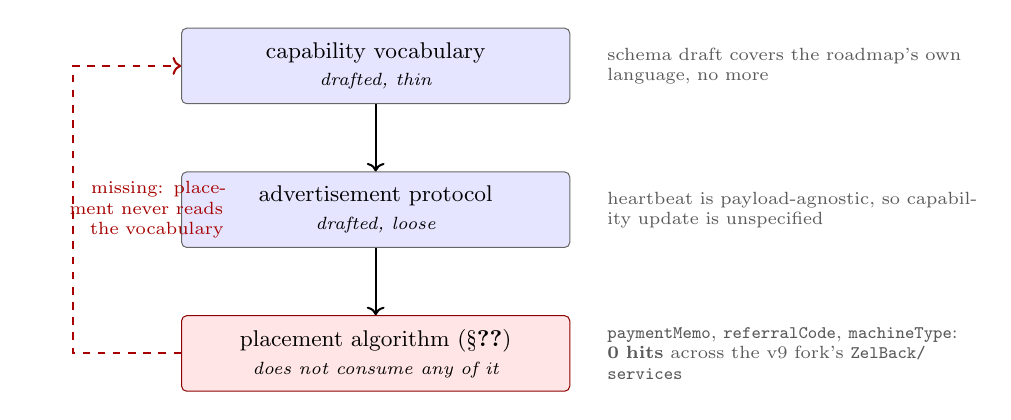
\begin{tikzpicture}[font=\small,
  box/.style={draw=black!60, rounded corners=2pt, minimum width=5.4cm, minimum height=1.05cm,
              align=center, inner sep=4pt},
  thin/.style ={box, fill=blue!10},
  loose/.style={box, fill=blue!10},
  none/.style ={box, fill=red!10, draw=red!55!black},
  note/.style ={font=\scriptsize, text=black!65, align=left, text width=5.1cm},
]
\node[thin]  (a) at (0,2.6) {capability vocabulary\\{\scriptsize\itshape drafted, thin}};
\node[loose] (b) at (0,0.6) {advertisement protocol\\{\scriptsize\itshape drafted, loose}};
\node[none]  (c) at (0,-1.4) {placement algorithm (\S\ref{sec:fluxos-placement})\\{\scriptsize\itshape does not consume any of it}};

\draw[->, thick] (a) -- (b);
\draw[->, thick] (b) -- (c);

% the missing feedback edge
%% Routed left: on the right it crossed the three grey annotation notes.
\draw[->, dashed, red!65!black, thick]
  (c.west) -- ++(-1.5,0) |- (a.west);
\node[font=\scriptsize, text width=2.6cm, align=right, text=red!65!black, anchor=east]
  at (-2.0,0.6) {missing: placement never reads the vocabulary};

\node[note, anchor=west] at (3.1,2.6)
  {schema draft covers the roadmap's own language, no more};
\node[note, anchor=west] at (3.1,0.6)
  {heartbeat is payload-agnostic, so capability update is unspecified};
\node[note, anchor=west] at (3.1,-1.4)
  {\texttt{paymentMemo}, \texttt{referralCode}, \texttt{machineType}: \textbf{0 hits} across the v9 fork's \texttt{Zel\allowbreak{}Back/\allowbreak{}services}};
\end{tikzpicture}

\caption{The three components a capability-typed provider runtime requires, and which of them exist
today.}
\end{figure}

\subsection{The datacenter tier and the field that names it}

The roadmap states its position on uniform capacity plainly, under the heading ``What we are not
doing'': ``\,`VPS on every node' in this cycle'' is rejected because ``home connections cannot serve
it reliably. The datacenter tier is what we can do properly now''
\srcroadmap{flux-roadmap-public.md:208}. That sentence has an architectural consequence the roadmap
does not spell out: a fleet that includes both home-connection Cumulus nodes and purpose-built
datacenter capacity is explicitly heterogeneous, and a specification that wants to route a workload
to one class and not the other has to say so. That is what \texttt{machineType} is for — a field on
the tenant side of the v9 schema that names \texttt{standard}, \texttt{gpu}, or \texttt{vps} as the
class of machine a deployment requires (\inprogress, \srccode{flux-spec/\allowbreak{}schema/\allowbreak{}v9.json}{79-82}).

The field is declared and unconsumed. As established above and in Section~10, \texttt{machineType}
has zero consumer code anywhere in \FluxOS, in either the organisation repository or its more mature
external fork. The VPS tier the roadmap schedules for H1~2027 is stated to depend on this exact flag
\srcroadmap{flux-roadmap-public.md:124-125}, and is itself gated behind the Q4~2026 operator-protection
work \srcroadmap{flux-roadmap-public.md:125}. So the tier has a name in the schema and nothing behind
it: no scheduling logic reads \texttt{machineType}, no node advertises which value it satisfies, and
no enforcement height is yet configured in \FluxOS{} for the specification version that carries the field, although one is now decided
(Section~10). Section~\ref{sec:feasibility} should carry this forward as one of the concrete, enumerable gaps between
the roadmap's dependency chain and what the code implements, rather than as a vague ``not yet
finished.''

\subsection{What convergence costs}

A single provider runtime is not free to build and would not be free to operate. The case for it is
real: one registration schema, one heartbeat mechanism, and one placement algorithm mean one code
path to secure and one place to add a new capability, instead of maintaining parity between \FluxOS's
gossip-based spawn loop and \FluxEdge's Kubernetes reconciler independently. A tenant who can express
\texttt{machine\allowbreak{}Type:\allowbreak{}~gpu} once and have it satisfied by whichever runtime currently holds the right
hardware gains something no product-level merge can deliver on its own — portability across a
heterogeneous fleet instead of a choice between two separately-billed products. The roadmap's ``payment
is the account, and per-second GPU without an account'' framing depends on exactly this: it is stated
to work ``with \FluxEdge folded into the platform'' \srcroadmap{flux-roadmap-public.md:79}, i.e. it
assumes the runtime-level unification this section has just shown is not yet designed.

The cost is that a single interface is shaped by its weakest supported node class. If the capability
vocabulary and placement algorithm are built to serve both a home-connection Cumulus node and a
datacenter-tier machine through one schema, either the interface degrades toward what the weaker class
can honestly promise, or the schema grows enough branching (as \texttt{machineType} already begins to
do) that ``one runtime'' becomes, in practice, several code paths gated by a flag — which is close to
where \FluxOS and \FluxEdge already are, just inside one repository instead of two. A home-connection
node and a datacenter node do not share a failure model: the roadmap's own reasoning for rejecting
``VPS on every node'' is precisely that home connectivity cannot be relied on for a workload class that
assumes always-on reachability \srcroadmap{flux-roadmap-public.md:208}. Any placement algorithm that
consumes capability flags has to encode that asymmetry correctly, or a tenant who requested
\texttt{vps} could in principle land on hardware whose network characteristics were never meant to
carry it — precisely the failure the tier distinction exists to prevent, and precisely the risk of
declaring a capability vocabulary before the placement algorithm that must honour it has been
designed.

\subsection{Vertical integration, argued both ways}

Flux controls the chain (\fluxd), the orchestration daemon (\FluxOS), and the attested host
(\ArcaneOS). One party controlling all three makes a guarantee reachable that no single-layer actor
could build alone: call it attested placement — a tenant's payment names a specific workload, \FluxOS
records which node placed it, and \ArcaneOS attests that the node booted a known-good image, with all
three artifacts meeting inside interfaces one party authors end to end.

No shipped mechanism assembles that chain today, and each leg is weaker than the phrase suggests.
The first leg does not yet exist: today a payment settles to a fixed transparent sink address and does
not reach the machine running the workload at all — the roadmap states this directly, ``today when
someone pays to run an application, that payment does not reach the machine running it''
\srcroadmap{flux-roadmap-public.md:111-112} — and binding a payment to a specific workload is exactly
what the PNR~v2 \texttt{paymentMemo} field is for (\planned; Section~7). The second leg is real but
off-chain: \FluxOS's placement decision is recorded in gossiped, signed messages, not on the chain
itself. The third leg exists but is weaker than ``attests the host'' implies: \ArcaneOS's attestation
service already defines a purpose-scoped signing key for exactly this use — a \texttt{purpose=app}
key sits alongside the existing, unconsumed \texttt{purpose=\allowbreak{}mesh} key
(\shipped, \srccode{fluxsas/\allowbreak{}src/\allowbreak{}api\_server.h}{411-481}) — but the signing material for every purpose
is derived by HKDF from salt and domain values compiled identically into every binary, not from
anything TPM- or machine-specific, so the attestation demonstrates that the signer holds a value
shipped in every copy of the software, not that a particular machine booted a particular image; there
is also no tenant-facing verification path today, since every attestation route requires an internal
mTLS client certificate bound to loopback. So ``attests the host'' is, at present, a Flux-operated
assurance a tenant cannot independently check, not a hardware-rooted one. The three names — the
payment-memo field, the placement gossip message, the attestation purpose token — are each Flux's own
schema decision; only a single controlling party is positioned to make them interoperate at all, which
is the sense in which the guarantee is uniquely reachable through vertical integration. Whether it is
actually reachable depends on work none of which has shipped: \vision, \srcinferred.

The same integration that makes this reachable has already foreclosed something else. The PoN block
header carries a fixed chainwork contribution per block regardless of difficulty
(\srccode{fluxd/\allowbreak{}src/\allowbreak{}pow.cpp}{284-290}), and a 2-of-4 emergency key set can produce a valid block
outside normal consensus rules. A header format chosen to make PoN's collateral-and-eligibility
sortition work is the same header format a light client on another chain would need to verify Flux
independently — and it cannot: without a commitment to the node set, without cumulative work to
compare forks by, and with an emergency path that can override normal validity, no light-client rule
derived from this header is sound. The most trust-minimising bridge architecture available to other
chains is closed to Flux until the header changes \srcintent{plan/mech-bridge.md, \S22}. That is the
same asymmetry as the attested-placement argument, run in the other direction: a design decision made
because one party controlled the whole stack, for one purpose, closed an option for a different
purpose that a less integrated system might have kept open. Integration is not, on this evidence, a
virtue or a defect on net; it is a set of coupled decisions with gains on one axis and closed doors on
another, and this section states both rather than choosing one.

\subsection{What would make convergence checkable}

Three things would turn this from an architectural claim into a testable one. First, a published
capability vocabulary — not the three-flag \texttt{capabilities} object and the three-value
\texttt{machineType} enum as they stand, but a vocabulary that actually covers GPU class, network
grade and storage durability, published somewhere a second implementation could target without
vendoring a private repository. Second, a placement algorithm — whether a revision of Section~9's
spawn loop or a successor — that reads that vocabulary when choosing a node, rather than the current
mechanism, which ignores every field convergence would depend on. Third, an enforcement height in the shipped configuration: v9 has
none today, though Section~10 records the one the team has settled on, and neither the provider-runtime contract nor the application schema that
carries \texttt{machineType} becomes binding on the network until one is set. Until all three exist,
``one platform'' describes an intent the roadmap has stated clearly and a runtime the code has not yet
built.

%% Drain this section's float queue before the next begins.
\FloatBarrier

\section{Networking and addressing: \FDM, \PDNS, mesh resolution, and private deployments}
\label{sec:networking}

An operator can point a browser or an API client at an application running somewhere on the
several-thousand-node \Flux fleet and get an answer. That works today, and the path by which it
works is worth naming precisely, because every hop on it is presently operated by the \Flux
Foundation. This is not a claim about node operators: the compute itself is dispersed across
independent Cumulus, Nimbus and Stratus operators exactly as advertised. It is a claim about
\emph{reachability} — DNS resolution, TLS termination, and the reverse proxy that decides which
container answers a given hostname all run on Foundation-controlled infrastructure, discovered
through a single Foundation-operated API with no on-chain or peer-to-peer fallback. Naming this
path precisely, hop by hop, is what makes the decentralization roadmap in \S\ref{sec:governance}
and elsewhere legible: a reader cannot evaluate a plan to decentralize a system without first
knowing exactly what is centralized in it today.

\subsection{The reachability path, end to end}
\label{sec:networking-path}

Application placement itself is decided elsewhere, by \FluxOS (\S\ref{sec:fluxos}); nothing in
this section governs \emph{where} an application runs. What this section governs is how a client
finds the IP:port that \FluxOS placed it on. \shipped

\begin{enumerate}
  \item \textbf{Discovery.} \FDM (\texttt{flux-\allowbreak{}domain-\allowbreak{}manager}) does not talk to \fluxd or to any
  peer-to-peer layer to learn what applications exist or where they run. It polls a single
  Flux-Foundation-operated REST API, \texttt{https:/\allowbreak{}/\allowbreak{}api.\allowbreak{}runonflux.\allowbreak{}io}, for
  \texttt{apps/\allowbreak{}globalappsspecifications} and \texttt{apps/locations}
  \srccode{flux-domain-manager/\allowbreak{}src/\allowbreak{}services/\allowbreak{}flux/\allowbreak{}dataFetcher.js}{47-71}. This is FDM's only
  source for "what apps exist and where"; no fallback source exists in the codebase
  \srccode{flux-domain-manager/\allowbreak{}src/\allowbreak{}services/\allowbreak{}flux/\allowbreak{}dataFetcher.js}{47-91}.
  \item \textbf{Polling cadence.} Three independent, self-rescheduling timers run per FDM process:
  \texttt{globalAppSpecs} at a default 30{,}000\,ms (conditional on HTTP \texttt{ETag}), \texttt{
  apps\allowbreak{}Locations} hardcoded to 10{,}000\,ms regardless of change, and \texttt{permMessages} at a
  default 120{,}000\,ms \srccode{flux-domain-manager/\allowbreak{}src/\allowbreak{}services/\allowbreak{}flux/\allowbreak{}dataFetcher.js}{47-91,409-417,689-721}.
  \item \textbf{Naming.} For a native application $\app$ with port $P$, FDM computes
  \texttt{$\app$\_$P$.app2.runonflux.io} (per port) and \texttt{$\app$.app2.runonflux.io} (main
  alias) by string concatenation — \texttt{app.} rather than \texttt{app2.} on the production
  shard \srccode{flux-domain-manager/\allowbreak{}src/\allowbreak{}services/\allowbreak{}domain/\allowbreak{}index.js}{9-32}. An operator may also
  set a custom domain in the application spec, which FDM verifies against its own IP via
  \texttt{dns.resolve4} before requesting a certificate for it
  \srccode{flux-domain-manager/\allowbreak{}src/\allowbreak{}services/\allowbreak{}domain/\allowbreak{}cert.js}{128-157}.
  \item \textbf{DNS.} A hostname is served either by Cloudflare, used strictly as authoritative
  "DNS-only" (grey-cloud) DNS — FDM actively deletes any record it finds with \texttt{proxied =\allowbreak{}=\allowbreak{}=\allowbreak{}
  true} — or by the self-hosted \PDNS zone service, selected per FDM host by
  \texttt{config.\allowbreak{}cloudflare.\allowbreak{}enabled}\slash\texttt{config.\allowbreak{}p\allowbreak{}DNS.\allowbreak{}enabled}
  \srccode{flux-domain-manager/\allowbreak{}src/\allowbreak{}services/\allowbreak{}domain/\allowbreak{}cert.js}{170-181}
  \srccode{flux-domain-manager/\allowbreak{}config/\allowbreak{}default.js}{32-47}. The evidence surveyed establishes how
  each backend behaves but not, from code alone, which one is authoritative for
  \texttt{runonflux.io} at any given moment: the checked-in default config is itself a
  certificate-only variant with \texttt{cloudflare.enabled:\ true}, and per-host Ansible
  templating can override this per fleet member \srccode{flux-domain-manager/\allowbreak{}config/\allowbreak{}default.js}{38,46}.
  \item \textbf{TLS termination and routing.} The FDM host's own \texttt{HAProxy} instance
  terminates TLS, binding \texttt{*:443} against every \texttt{.pem} file under
  \texttt{/\allowbreak{}etc/\allowbreak{}ssl/\allowbreak{}fluxapps/\allowbreak{}} \srccode{flux-domain-manager/\allowbreak{}src/\allowbreak{}services/\allowbreak{}haproxyTemplate.js}{81-134},
  then routes on the \texttt{Host} header via an ACL to the matching backend, forwarding to one of
  the application's container IPs at its declared port
  \srccode{flux-domain-manager/\allowbreak{}src/\allowbreak{}services/\allowbreak{}haproxyTemplate.js}{260-319}. Per-server health
  checks (\S\ref{sec:networking-runloop}) decide which of an application's IPs are actually in that
  backend at any moment.
  \item \textbf{Game-application shortcut.} For roughly two dozen "G-mode" game-server application
  types (Minecraft, Rust, Valheim, and similar), a separate, single-instance service,
  \texttt{flux-\allowbreak{}apps-\allowbreak{}dns-\allowbreak{}manager}, reads the master IP FDM already elected into its own
  \texttt{/appips} output and publishes it directly as an \texttt{A} record via the DNS Gateway
  (\S\ref{sec:networking-gateway}) — client traffic, often UDP, goes node-to-node and never passes
  through HAProxy \srccode{flux-apps-dns-manager/\allowbreak{}src/\allowbreak{}services/\allowbreak{}appsDnsManager.js}{202-255}
  \srcdoc{flux-apps-dns-manager/README.md:3-15}.
\end{enumerate}

\begin{figure}[H]
  \centering
  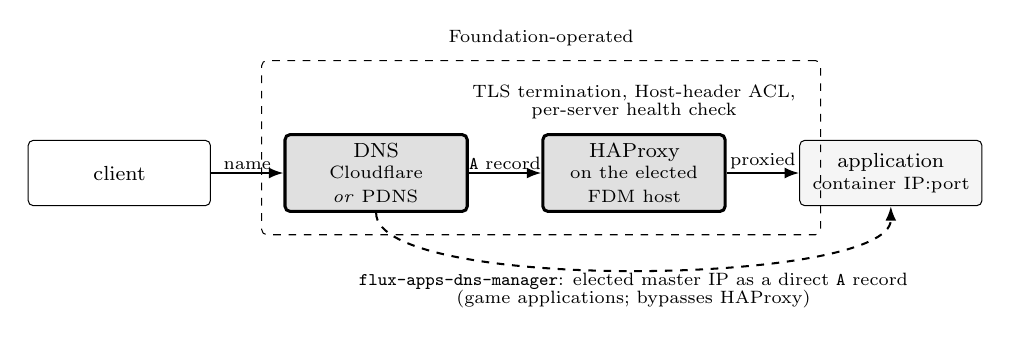
\begin{tikzpicture}[
    font=\footnotesize,
    node distance=6mm,
    box/.style={draw, rounded corners=2pt, minimum height=9mm, align=center,
                inner xsep=3pt, text width=23mm},
    flux/.style={box, fill=black!4},
    found/.style={box, fill=black!12, very thick},
    lbl/.style={font=\scriptsize, align=center, inner sep=1pt},
    arr/.style={-{Latex[length=2mm]}, thick},
  ]
    \node[box]   (client) {client};
    \node[found, right=10mm of client] (dns) {DNS\\[-1pt]{\scriptsize Cloudflare \emph{or} \PDNS}};
    \node[found, right=10mm of dns]    (ha)  {HAProxy\\[-1pt]{\scriptsize on the elected \FDM host}};
    \node[flux,  right=10mm of ha]     (app) {application\\[-1pt]{\scriptsize container IP:port}};

    \draw[arr] (client) -- node[lbl, above] {name} (dns);
    \draw[arr] (dns) -- node[lbl, above] {\texttt{A} record} (ha);
    \draw[arr] (ha)  -- node[lbl, above] {proxied} (app);

    % HAProxy-bypassing shortcut for game applications
    \draw[arr, dashed] (dns.south) .. controls +(0,-11mm) and +(0,-11mm) ..
      node[lbl, below, pos=0.5] {\texttt{flux-\allowbreak{}apps-\allowbreak{}dns-\allowbreak{}manager}: elected master IP as a direct
        \texttt{A} record\\[-1pt](game applications; bypasses HAProxy)} (app.south);

    %% Named and included in the fit: as a bare label above `ha' it printed on top of
    %% the dashed box's own "Foundation-operated" label, which sits at the same height.
    \node[lbl, above=1.5mm of ha] (tls) {TLS termination, Host-header ACL,\\[-1pt]per-server health check};
    \node[draw, dashed, rounded corners=2pt, inner sep=3mm, fit=(dns)(ha)(tls),
          label={[lbl, yshift=1.5mm]above:{Foundation-operated}}] {};
  \end{tikzpicture}
  \caption{The reachability path from client to a running application, and the game-application
  shortcut that bypasses \FDM's HAProxy entirely. Both intermediate hops are Foundation-operated
  \shipped; \S\ref{sec:networking-inventory} inventories what each depends on and what happens
  when it is unavailable.}
  \label{fig:reachability-path}
\end{figure}

The \texttt{*.\allowbreak{}app.\allowbreak{}runonflux.\allowbreak{}io}\slash\texttt{*.\allowbreak{}app2.\allowbreak{}runonflux.\allowbreak{}io} wildcard certificate that step 5
depends on is treated by \FDM's own code as always present — the presence check short-circuits to
\texttt{true} for any domain ending in these suffixes, so \FDM never calls \texttt{certbot} for
them \srccode{flux-domain-manager/\allowbreak{}src/\allowbreak{}services/\allowbreak{}domain/\allowbreak{}cert.js}{18-22}.
\decided{the wildcard certificate is managed by InFlux Technologies USA LLC and renewed
periodically against the \texttt{runonflux.io} domain \srcintent{08-answers-round-2.md, rounds
24--25}. This is less of a concentration than it first reads. Behind any certificate there must be
some company managing the domain --- that is a property of the web PKI rather than of \Flux{} --- and
what matters is whether the arrangement can be replicated. It can: \texttt{flux-domain-manager} is
public under AGPL-3.0, the application specification already admits tenant-set custom domains
\srccode{flux/\allowbreak{}ZelBack/\allowbreak{}src/\allowbreak{}services/\allowbreak{}appsService.js}{passim}, and any operator may run
their own \FDM{}, their own \PDNS{} and serve applications from a domain they control.

Discovery is replicable too, and this paper's earlier reading of
\texttt{api.\allowbreak{}runonflux.\allowbreak{}io} conflated two different claims. The endpoint is not a
Foundation-only service: \texttt{/apps/\allowbreak{}globalappsspecifications} is an ordinary \FluxOS{}
route served by \emph{every} node \shipped~\srccode{flux/\allowbreak{}ZelBack/\allowbreak{}src/\allowbreak{}routes.js}{402}, and
\FDM{} takes its host as a constructor parameter, \texttt{flux\allowbreak{}Api\allowbreak{}BaseUrl}, whose
shipped value merely happens to be that name
\shipped~\srccode{flux-domain-manager/\allowbreak{}src/\allowbreak{}services/\allowbreak{}flux/\allowbreak{}dataFetcher.js}{886}. Pointing an
independent \FDM{} at any of the \num{6489} nodes, or at a bare IP, is a configuration change rather
than a fork --- and the code is AGPL-3.0 if a fork is wanted anyway.

What survives is narrower and is a resilience property, not a centralisation one: as shipped there is
\emph{one} base URL and \emph{no automatic failover}, so an \FDM{} whose configured endpoint becomes
unreachable stalls on its last-known data rather than trying another node. That is worth fixing and
is recorded in \Cref{tab:centralization} on those terms. \textbf{What is centralised here is the
default, not the capability.}}

\subsection{\FDM's run loop}
\label{sec:networking-runloop}

\FDM's inputs are the three polled feeds above (application specs, locations, permanent
messages); its output is a generated \texttt{HAProxy} configuration file, validated with
\texttt{haproxy -\allowbreak{}f .\allowbreak{}.\allowbreak{}.\allowbreak{} -\allowbreak{}c} before it is ever installed — a failed validation leaves the
previously-loaded configuration serving, not a hard outage
\srccode{flux-domain-manager/\allowbreak{}src/\allowbreak{}services/\allowbreak{}domainService.js}{196-200,355-359}
\srccode{flux-domain-manager/\allowbreak{}src/\allowbreak{}services/\allowbreak{}haproxyTemplate.js}{626-646}. Reconfiguration of the
main HAProxy pool (the \texttt{home}\slash\texttt{api}\slash\texttt{cloud} UI/API backends) is driven purely
by a 30{,}000\,ms self-rescheduling timer, independent of any external event
\srccode{flux-domain-manager/\allowbreak{}src/\allowbreak{}services/\allowbreak{}domainService.js}{96-210}; that regeneration throws and
aborts the cycle if fewer than 10 Stratus candidates pass its 8-stage health chain, keeping the
old configuration running rather than publishing an under-populated pool
\srccode{flux-domain-manager/\allowbreak{}src/\allowbreak{}services/\allowbreak{}domainService.js}{110-183}. Reconfiguration of
per-application backends is driven by the \texttt{apps\allowbreak{}Locations\allowbreak{}Updated} event fired on every
10-second location poll, which re-checks every location IP with a per-application-type coded
health check and writes into the backend only the IPs that pass
\srccode{flux-domain-manager/\allowbreak{}src/\allowbreak{}services/\allowbreak{}domainService.js}{730-767}. \shipped

\begin{table}[H]
\centering
\small
\renewcommand{\arraystretch}{1.15}
\caption{\FDM/\PDNS reachability-path health-check and reconfiguration constants.}
\label{tab:fdm-health-constants}
\begin{tabular}{lll}
\toprule
Mechanism & Constants & Source \\
\midrule
Generic app backend, HAProxy-level & \texttt{inter 3s fall 2 rise 2 fastinter 500} & \srccode{flux-domain-manager/\allowbreak{}src/\allowbreak{}services/\allowbreak{}haproxyTemplate.js}{311} \\
\quad detection floor & $\approx$6\,s down (2$\times$3\,s) & \srccode{flux-domain-manager/\allowbreak{}src/\allowbreak{}services/\allowbreak{}haproxyTemplate.js}{311} \\
Main UI/API backend, HAProxy-level & \texttt{inter 10s fall 2 rise 3 maxconn 100} & \srccode{flux-domain-manager/\allowbreak{}src/\allowbreak{}services/\allowbreak{}haproxyTemplate.js}{384,408,427} \\
\quad detection floor & $\approx$20\,s down, 30\,s up & \srccode{flux-domain-manager/\allowbreak{}src/\allowbreak{}services/\allowbreak{}haproxyTemplate.js}{384,408,427} \\
G-mode sticky-master retries & 3 attempts, 3{,}000\,ms apart & \srccode{flux-domain-manager/\allowbreak{}src/\allowbreak{}services/\allowbreak{}domainService.js}{29-30} \\
G-mode sticky-unhealthy grace & 90{,}000\,ms since last healthy & \srccode{flux-domain-manager/\allowbreak{}src/\allowbreak{}services/\allowbreak{}domainService.js}{31} \\
\texttt{appsLocations} poll (control plane) & 10{,}000\,ms, hardcoded & \srccode{flux-domain-manager/\allowbreak{}src/\allowbreak{}services/\allowbreak{}flux/\allowbreak{}dataFetcher.js}{66,707} \\
Main HAProxy pool regeneration & 30{,}000\,ms, self-rescheduling & \srccode{flux-domain-manager/\allowbreak{}src/\allowbreak{}services/\allowbreak{}domainService.js}{201-208} \\
Main pool minimum candidates & 10 (throws below this) & \srccode{flux-domain-manager/\allowbreak{}src/\allowbreak{}services/\allowbreak{}domainService.js}{181-183} \\
CDM certificate obtain/renew loop & 15\,min (900{,}000\,ms) & \srccode{flux-domain-manager/\allowbreak{}src/\allowbreak{}services/\allowbreak{}domainService.js}{1046-1088} \\
\bottomrule
\end{tabular}
\end{table}

Because the G-mode control-plane grace window (90\,s) is a much slower mechanism than HAProxy's
own data-plane health check ($\approx$6\,s detection floor), an already-open connection to a dead
sticky IP typically stops receiving traffic within HAProxy's own $\approx$6--9\,s window; the 90\,s
constant instead bounds how long \FDM keeps re-publishing the same, possibly-dead IP into the
configuration before attempting election of a new one
\srccode{flux-domain-manager/\allowbreak{}src/\allowbreak{}services/\allowbreak{}domainService.js}{253-321}. \shipped

\subsection{Certificates}
\label{sec:networking-certs}

Every certificate in this path is issued by Let's Encrypt, exclusively, via \texttt{certbot
certonly -\allowbreak{}-\allowbreak{}standalone -\allowbreak{}-\allowbreak{}http-\allowbreak{}01-\allowbreak{}port=8787}
\srccode{flux-domain-manager/\allowbreak{}src/\allowbreak{}services/\allowbreak{}domain/\allowbreak{}cert.js}{38-46}; no wildcard issuance is coded —
only exact-domain HTTP-01 challenges. The ACME account state (keys, order history) lives wherever
\texttt{certbot} itself keeps it, under \texttt{/\allowbreak{}etc/\allowbreak{}letsencrypt/\allowbreak{}}, outside \FDM's own code. The
artifact \texttt{HAProxy} actually serves is a single, world-readable-by-haproxy file per domain,
\texttt{/etc/ssl/\{certFolder\}/\{domain\}.pem}, formed by concatenating \texttt{fullchain.pem}
and \texttt{privkey.pem} — public certificate and private key in one file
\srccode{flux-domain-manager/\allowbreak{}src/\allowbreak{}services/\allowbreak{}domain/\allowbreak{}cert.js}{38-46}
\srccode{flux-domain-manager/\allowbreak{}src/\allowbreak{}services/\allowbreak{}haproxyTemplate.js}{141-150}. \shipped

Issuance is technically permissionless: any host that can bind port 8787 for the HTTP-01
challenge and run \texttt{sudo certbot} can obtain a certificate for a domain it is authoritative
for. Operationally, in the deployed fleet, only the 16 Flux-Foundation-run \FDM/CDM hosts ever do
so; an ordinary Cumulus, Nimbus or Stratus node operator never runs \FDM or its certificate-only
sibling \srccode{flux-fdm-infrastructure/\allowbreak{}ansible/\allowbreak{}inventory/\allowbreak{}hosts.yaml}{1-100}. Two PM2 processes
run from the same repository on the per-shard app hosts: \texttt{FDM} itself
(\texttt{manage\allowbreak{}Certificate\allowbreak{}Only:\allowbreak{} false}, handles HAProxy) and, on the EU-private-network hosts, a
second clone named \texttt{CDM} ("cert-domain-manager", \texttt{manage\allowbreak{}Certificate\allowbreak{}Only:\allowbreak{} true}),
dedicated purely to issuance and renewal
\srccode{flux-domain-manager/\allowbreak{}deployment/\allowbreak{}fdm\_setup.yml}{1-9,140-259}. CDM's loop runs every
15\,min, classifying each custom domain into skip/obtain/renew — renewing when fewer than 30 days
of validity remain — and deleting any certificate that expired more than 30 days ago
\srccode{flux-domain-manager/\allowbreak{}src/\allowbreak{}services/\allowbreak{}domain/\allowbreak{}cert.js}{18-36,91-126,214-249,308-340}. \shipped

\subsection{\fluxdnsd mesh resolution: a local file-tail resolver, not a gossip protocol}
\label{sec:networking-dnsd}

The name \fluxdnsd invites a reading in which nodes discover each other's application members by
talking to one another — a gossip or peer-to-peer resolution protocol. That reading is wrong, and
the paper states this plainly because the mistake is an easy one to make from the name alone.
\fluxdnsd is a purely local, single-node process. It holds an in-memory view built from exactly one
JSON file, \texttt{/\allowbreak{}var/\allowbreak{}lib/\allowbreak{}flux-mesh/\allowbreak{}resolver/\allowbreak{}membership.\allowbreak{}json}, and answers
\texttt{*.mesh.flux} queries from that view, scoped to the querying container's source IP
\srccode{flux-dnsd/\allowbreak{}src/\allowbreak{}snapshot.rs}{319-363,79-84}. It never opens a connection to another
\fluxdnsd instance, never queries a central server at request time, and implements no notion of
node-to-node consensus \srccode{flux-dnsd/\allowbreak{}src/\allowbreak{}snapshot.rs}{319-363}. The file is written by
\FluxOS, which computes the per-node membership view and installs it with a temporary-file-then-
rename, an atomic operation \fluxdnsd's file watcher depends on: only an inotify
\texttt{IN\_MOVED\_TO} event whose destination is \texttt{membership.\allowbreak{}json} triggers a reload —
a plain write-in-place is inert by construction
\srccode{flux-dnsd/\allowbreak{}src/\allowbreak{}watcher.rs}{20-69}. As the component's own documentation states,
"FluxOS's database is the authority and rewrites it on boot-sync"
\srcdoc{flux-dnsd/README.md:75-85}. \shipped

The cross-node propagation that makes membership on one node visible to a container on another —
the actual mechanism a reader might expect "mesh" to name — happens entirely inside \FluxOS,
outside \fluxdnsd. From \fluxdnsd's own source this propagation mechanism is opaque: the daemon
"only accepts or rejects [the file] whole," never repairing, merging, or arbitrating between
disagreeing sources \srcdoc{flux-dnsd/README.md:83-85}
\srccode{flux-dnsd/\allowbreak{}src/\allowbreak{}snapshot.rs}{72-77}. A snapshot whose generation number does not strictly
exceed the currently loaded view's is rejected outright, so a stale or replayed file cannot
regress the served view \srccode{flux-dnsd/\allowbreak{}src/\allowbreak{}snapshot.rs}{397-416}. Answers carry a fixed
5-second TTL, justified in the source as "membership changes must propagate and nothing in the
path caches anyway" \srccode{flux-dnsd/\allowbreak{}src/\allowbreak{}main.rs}{57-60}. If no valid snapshot has ever
arrived, or the source IP is unscoped, the daemon answers \texttt{REFUSED} rather than
\texttt{SERVFAIL}\slash\texttt{NXDOMAIN}, so a client's stub resolver fails over to its secondary
nameserver \srccode{flux-dnsd/\allowbreak{}src/\allowbreak{}server.rs}{82-90}. \shipped

\subsection{flux-dns-gateway: an mTLS proxy in front of the \PDNS key}
\label{sec:networking-gateway}

\texttt{flux-\allowbreak{}dns-\allowbreak{}gateway} is an mTLS-fronted proxy that lets the 16 \FDM instances write DNS
records into \PDNS without any of them ever holding the \PDNS API key themselves
\srcdoc{flux-dns-gateway/README.md:1-29}. Nginx terminates and verifies the client certificate and
sets \texttt{X-\allowbreak{}SSL-\allowbreak{}Client-\allowbreak{}Verify}\slash\texttt{X-\allowbreak{}SSL-\allowbreak{}Client-\allowbreak{}CN} headers that the FastAPI backend trusts
unconditionally, with no re-verification of the certificate itself in the Python layer
\srccode{flux-dns-gateway/\allowbreak{}src/\allowbreak{}dns\_gateway/\allowbreak{}api/\allowbreak{}middleware/\allowbreak{}auth.py}{18-69}. Each client's ACL is
enforced by \texttt{client\_cn}, \texttt{allowed\_zones}, \texttt{allowed\_record\_types}, and
\texttt{allowed\_prefixes}, deny-by-default for any unrecognised \texttt{client\_cn}
\srccode{flux-dns-gateway/\allowbreak{}src/\allowbreak{}dns\_gateway/\allowbreak{}config/\allowbreak{}acl.py}{13-97,99-151}. \shipped

The README's example ACL configuration also documents two further safety fields,
\texttt{max\_records\_per\_zone} and \texttt{rate\_limit\_per\_minute}
\srcdoc{flux-dns-gateway/README.md:259-274}. Neither has any corresponding reader anywhere in the
source: the \texttt{ACLConfig}\slash\texttt{FDMPermissions} parser reads only the four fields listed
above \srccode{flux-dns-gateway/\allowbreak{}src/\allowbreak{}dns\_gateway/\allowbreak{}config/\allowbreak{}acl.py}{21-30}. A documented per-zone
record cap and a documented per-client rate limit are, as deployed, no-ops. \shipped

\subsection{flux-geo-cert: a citation trap}
\label{sec:networking-geocert}

\texttt{flux-geo-cert}'s name and its corpus label ("Certificate Orchestrator for Flux Geo CDN")
suggest node-location attestation. It is not that. It is a Python service that automates Let's
Encrypt DNS-01 certificate renewal for the geo-routed CDN domain and pushes the resulting
certificates over SSH to a small set of CDN nodes (Germany, US, Hong Kong)
\srcdoc{flux-geo-cert/README.md:1-13}
\srccode{flux-fdm-infrastructure/\allowbreak{}ansible/\allowbreak{}inventory/\allowbreak{}hosts.yaml}{155-177}. It has no inbound network
interface at all — "pure outbound service" \srcdoc{flux-geo-cert/ARCHITECTURE.md:54} — and
performs no measurement, claim, or signature about where any Flux node physically is. No code
anywhere in the repositories surveyed for this section implements cryptographic attestation of
node geography; the geolocation machinery that actually feeds placement decisions
(fault-domain counting, residential-versus-hosting classification) lives in
\texttt{fluxos-\allowbreak{}network-\allowbreak{}policy}'s \texttt{iplocation.\allowbreak{}bin.\allowbreak{}gz} artifact
(\S\ref{sec:networking-policy}), a build-time table sourced from RIR delegated-extended files and
commercial geolocation data, not from any on-node measurement. This paper does not cite
\texttt{flux-geo-cert} for, and makes no claim anywhere that, node geography is cryptographically
attested.

\subsection{fluxos-network-policy: the governance-relevant lever}
\label{sec:networking-policy}

\texttt{fluxos-\allowbreak{}network-\allowbreak{}policy} is a small set of JSON/binary documents — blocked repositories,
vetted repositories, a tampering blocklist, an enterprise-node owner allow-list, and a
$\sim$2.0-million-row IP$\to$(organisation, country, region) geolocation table — that every
\FluxOS node fetches on a fixed schedule over plain HTTPS and enforces immediately, fleet-wide,
with no staged rollout \srcdoc{fluxos-network-policy/README.md:1-9,11-17,30-44}. Fetch intervals
are 6\,h for the blocked-repositories and enterprise-node documents and 12\,h for the tampering
blocklist, with the geolocation table refreshed on a daily conditional check
\srcdoc{fluxos-network-policy/README.md:34-35}
\srccode{flux/\allowbreak{}ZelBack/\allowbreak{}src/\allowbreak{}services/\allowbreak{}utils/\allowbreak{}cacheManager.js}{126-129}
\srccode{flux/\allowbreak{}ZelBack/\allowbreak{}src/\allowbreak{}services/\allowbreak{}utils/\allowbreak{}enterpriseConfig.js}{12}
\srccode{flux/\allowbreak{}ZelBack/\allowbreak{}src/\allowbreak{}services/\allowbreak{}appTamperingBlocklistService.js}{11}. A node that cannot reach the repository keeps
enforcing whatever it last successfully fetched, indefinitely and across restarts — failure here
is neither fail-open nor fail-closed-to-empty but fail-frozen, and a node that has never
successfully fetched anything declines to answer rather than guess
\srcdoc{fluxos-network-policy/README.md:33-44}. \shipped

The documents are unsigned and served over plain HTTPS; by the component's own account, "their
authenticity rests on GitHub and on who can merge to this repo"
\srcdoc{fluxos-network-policy/README.md:320-326}. Write access is restricted to GitHub
organisation owners, and there is deliberately no second-reviewer requirement: CI runs a shape
validator and a dual-write mirror check only, reaching green in roughly 15 seconds, after which
the author of the pull request may merge their own change
\srcdoc{fluxos-network-policy/README.md:297-303}
\srccode{fluxos-network-policy/\allowbreak{}.github/\allowbreak{}CODEOWNERS}{1-7}
\srccode{fluxos-network-policy/\allowbreak{}.github/\allowbreak{}workflows/\allowbreak{}validate.yml}{1-27}. The stated reasoning is
explicit: "the moment you most need to change policy is during an incident, and a rule requiring a
second person is one that gets bypassed at 3am"
\srcdoc{fluxos-network-policy/README.md:300-302}. Once merged, every \FluxOS node enforces
the new document on its own next scheduled fetch — within 7--13\,h depending on the document, the
fetch interval plus the hourly sweep (\S\ref{sec:governance}), with
no canary and no staged rollout \srcdoc{fluxos-network-policy/README.md:3-5,34-35}. \shipped

Concretely, a single merged pull request can: block or unblock any container image, namespace,
owner address, or 64-hex application hash network-wide (\texttt{blockedrepositories.\allowbreak{}json},
\texttt{vettedrepositories.\allowbreak{}json}); grant or revoke which owner addresses may install applications
on which enterprise-designated nodes (\texttt{enterprisenodes.\allowbreak{}json}); mark a node's collateral
transaction hash as blocked for tampering (\texttt{tamperingblockednodes.\allowbreak{}json}), a mechanism the
evidence describes as able to DOS a node's collateral for that offense; and, via the monthly
geolocation-baseline pull request, reclassify which organisations or regions count as residential
versus hosting for placement fault-domain counting and enforcement purposes
\srcdoc{fluxos-network-policy/README.md:320-326,99-172}. This is, by the component's own
documentation, "the sharpest single point of centralized, unsigned control" identified across the
network- and addressing-plane components covered in this section
\srcdoc{fluxos-network-policy/README.md:320-326}; \S\ref{sec:governance} argues directly from this
lever when it assesses censorship- and Sybil-resistance at the measured node distribution. \shipped

\subsection{The centralization inventory}
\label{sec:networking-inventory}

Table~\ref{tab:centralization} states, without further comment, which surfaces described in this
section are Foundation-operated, what depends on each, and what happens if each is unavailable.

\begin{table}[H]
\centering
\small
\renewcommand{\arraystretch}{1.2}
\caption{Centralization surfaces in the reachability and naming path.}
\label{tab:centralization}
\begin{tabular}{p{2.6cm}p{2.1cm}p{4.4cm}p{4.6cm}}
\toprule
Surface & Operator & Depends on it & If unavailable \\
\midrule
\texttt{api.\allowbreak{}runonflux.\allowbreak{}io} (application discovery) --- the \emph{configured default},
not a unique source & Flux Foundation operates this endpoint; the route it serves is on every node & Every \FDM/CDM
control-plane loop reads app specs, locations and permanent messages from one configured base URL. The
route is an ordinary \FluxOS{} one served by all \num{6489} nodes \srccode{flux/\allowbreak{}ZelBack/\allowbreak{}src/\allowbreak{}routes.js}{402}
and the host is a constructor parameter \srccode{flux-domain-manager/\allowbreak{}src/\allowbreak{}services/\allowbreak{}flux/\allowbreak{}dataFetcher.js}{886},
so an independent operator repoints it by configuration & \textbf{Resilience, not centralisation:} no
automatic failover to another node is coded, so a loop whose configured endpoint is unreachable keeps
polling, logs errors and serves the last-known HAProxy configuration (fail-static)
\srccode{flux-domain-manager/\allowbreak{}src/\allowbreak{}services/\allowbreak{}flux/\allowbreak{}dataFetcher.js}{47-91} \\
\addlinespace
Foundation-private \texttt{10.100.0.0/24} (WireGuard hub, \PDNS masters, DNS Gateway, Arcane load
balancers, SAS decrypt endpoint) & Flux Foundation & All non-EU \FDM/CDM and
\texttt{flux-\allowbreak{}apps-\allowbreak{}dns-\allowbreak{}manager} instances, reachable outside the EU segment only through a single
WireGuard hub, \texttt{wireguard-\allowbreak{}eu-\allowbreak{}01} (\texttt{10.100.0.167}, public
\texttt{5.39.57.49:\allowbreak{}51000}) \srccode{flux-fdm-infrastructure/\allowbreak{}ansible/\allowbreak{}inventory/\allowbreak{}hosts.yaml}{180-185}
& Custom-domain certificate issuance, enterprise application-spec decryption, and game-application
DNS publication all stop for every host that reaches this segment only through that hub
\srccode{flux-domain-manager/\allowbreak{}src/\allowbreak{}services/\allowbreak{}domainService.js}{1099-1105} \\
\addlinespace
16-host \FDM/CDM fleet (6 EU direct-private, 6 US and 4 Singapore over WireGuard)
\srccode{flux-fdm-infrastructure/\allowbreak{}ansible/\allowbreak{}inventory/\allowbreak{}hosts.yaml}{1-100} & Flux Foundation & HAProxy
routing and TLS termination for every \texttt{app(2).\allowbreak{}runonflux.\allowbreak{}io} and custom-domain hostname
network-wide & Stale-but-serving: a failed configuration validation leaves the previous
configuration running, but no new application is routed or certified until a host recovers
\srccode{flux-domain-manager/\allowbreak{}src/\allowbreak{}services/\allowbreak{}domainService.js}{196-200} \\
\addlinespace
\texttt{flux-\allowbreak{}apps-\allowbreak{}dns-\allowbreak{}manager} (single, unreplicated instance on \texttt{flux-cert-1} =
\texttt{10.100.0.172}) & Flux Foundation & Direct node-to-node DNS for $\sim$26 G-mode
game-server application types
\srccode{flux-apps-dns-manager/\allowbreak{}config/\allowbreak{}gamesConfig.js}{30-57} & No coded high availability,
leader election, or standby process; game-application \texttt{A} records stop updating until the
single host/co-located DNS Gateway returns
\srccode{flux-apps-dns-manager/\allowbreak{}ansible/\allowbreak{}inventory.yaml}{6-7} \\
\addlinespace
Let's Encrypt (ACME certificate authority) & External (ISRG) & Every TLS-terminated
\texttt{app(2).\allowbreak{}runonflux.\allowbreak{}io} and custom-domain certificate; exclusively used, no alternate CA
coded \srccode{flux-domain-manager/\allowbreak{}src/\allowbreak{}services/\allowbreak{}domain/\allowbreak{}cert.js}{38-46} & No fallback CA; the CDM
renewal loop retries every 15\,min indefinitely, and the 30-day renewal floor provides slack, but
new domains cannot be certified at all during an outage \\
\addlinespace
Cloudflare (where \texttt{config.\allowbreak{}cloudflare.\allowbreak{}enabled}) & External (Cloudflare) & DNS resolution for
domains on the Cloudflare-selected path, used strictly DNS-only (grey-cloud), never as a proxy or
CDN \srccode{flux-domain-manager/\allowbreak{}src/\allowbreak{}services/\allowbreak{}domain/\allowbreak{}cert.js}{170-181} & No fallback registrar or
DNS backend is coded per domain; whichever hostnames are Cloudflare-hosted stop resolving \\
\bottomrule
\end{tabular}
\end{table}

\subsection{Node network configuration}
\label{sec:networking-nodeconfig}

At install and reconfiguration time, network interfaces are discovered automatically: a
\texttt{probert}-backed (netlink and udev) scan produces interface objects carrying type, name,
state, index, MAC, vendor, model, address, VLAN and bridge identifiers with no operator input
\srccode{fluxos-iso-networking-shared/\allowbreak{}src/\allowbreak{}flux\_networking\_shared/\allowbreak{}models/\allowbreak{}network.py}{326-388}.
What the operator configures, per interface, is the allocation mode — DHCP or static — through a
TUI screen; choosing static reveals a form for subnet, address, gateway and DNS that is
blur-validated before the change may be saved
\srccode{fluxos-iso-networking/\allowbreak{}src/\allowbreak{}flux\_iso\_networking/\allowbreak{}screens/\allowbreak{}interface\_modal\_screen.py}{54,79-84,200-284}.
Per-interface traffic shaping is likewise operator-set, from a closed set of rates
($\{35,75,135,250\}$\,Mbps), written to a policy file and applied by a separate, privileged D-Bus
helper because the configuring process itself runs without the capability to apply it directly
\srccode{fluxos-iso-networking-shared/\allowbreak{}src/\allowbreak{}flux\_networking\_shared/\allowbreak{}models/\allowbreak{}network.py}{77,83,139-161,224}.
\shipped

The stack is IPv4-only by construction, not merely by current deployment. Every network dataclass
— \texttt{Route}, \texttt{SourceAddress}, \texttt{NetworkInterface.\allowbreak{}address} — is typed
\texttt{IPv4Network}\slash\texttt{IPv4Address}\slash\texttt{IPv4Interface} and nothing else, and the shared
connectivity helper pins \texttt{TCPConnector(family=\allowbreak{}AF\_INET)} explicitly
\srccode{fluxos-iso-networking-shared/\allowbreak{}src/\allowbreak{}flux\_networking\_shared/\allowbreak{}models/\allowbreak{}network.py}{17-29,326-337}
\srccode{fluxos-iso-networking-shared/\allowbreak{}src/\allowbreak{}flux\_networking\_shared/\allowbreak{}helpers.py}{147,242}. The
measured fleet crawl underlying the network-wide baseline in \S\ref{sec:baseline} reports
2{,}322 IPv4 addresses and zero IPv6 or onion (Tor hidden-service) addresses
\srcmeasured{api.runonflux.io/\allowbreak{}daemon/\allowbreak{}getzelnodecount}{2026-09-03}. \shipped

A reachability design for NAT'd and non-public nodes exists only as a docstring. The helper
\texttt{is\_directly\_public()} states that a node with a globally-routable public IP bound to one
of its own interfaces would act as a "Tor SOCKS-only hub," while a NAT'd node would instead run a
"Tor hidden service" to become reachable
\srccode{fluxos-iso-networking-shared/\allowbreak{}src/\allowbreak{}flux\_networking\_shared/\allowbreak{}models/\allowbreak{}network.py}{461-479}.
No Tor-related code exists anywhere else in either the installer or the shared networking library;
the design is fully specified in prose and entirely unimplemented. \vision

\subsection{Private deployments (\VPON)}
\label{sec:networking-vpon}

The roadmap lists private deployments, referred to as \VPON s (private overlay networks), as a
Q4 2026 item, described as "the complement to private payments and chain privacy"
\srcroadmap{Private deployments (VPONs), Q4 2026}; the roadmap's own timeline artifact labels the
same item "Private overlay networks," sub-labelled "VPONs $\cdot$ private deployments"
\srcdoc{flux-roadmap/public/timeline.html:172-173}. No implementation of a \VPON was found in any
repository surveyed for this section or flagged elsewhere in the corpus; the roadmap evidence
itself notes no repository name observed anywhere in the codebase corresponds to a \VPON
\srcdoc{flux-roadmap/public/flux-roadmap-public.md:83}. \planned

Because no such system exists to describe, this section states what a \VPON would need to provide
rather than how one works. At minimum, consistent with the notation this paper uses for the term
and with the roadmap's framing of \VPON s as private overlays rather than a naming variant on the
public network:
\begin{itemize}
  \item \textbf{Membership by key, not by discoverability.} The reachability path in
  \S\ref{sec:networking-path} and the mesh namespace in \S\ref{sec:networking-dnsd} both resolve
  any application's members to any container scoped correctly on the querying node; a \VPON would
  need membership gated by possession of a private key rather than resolvable by any party who can
  reach the mesh namespace or the public API \srcinferred.
  \item \textbf{Reachability-plane confidentiality.} If a \VPON exists to complement private
  payment (\S\ref{sec:private-payment}) and chain privacy, then the infrastructure this section
  describes — the discovery API, \FDM, and \PDNS, all Foundation-operated — should not be
  positioned to learn which nodes host a private deployment or on whose behalf, since today's
  reachability path is Foundation-legible end to end by the construction in
  \S\ref{sec:networking-path} \srcinferred.
\end{itemize}
The roadmap sequences \VPON s alongside private payments and the chain-privacy work without
stating an explicit blocking dependency between them
\srcdoc{flux-roadmap/public/flux-roadmap-public.md:81,84}. Beyond this framing, no wire protocol,
key-management scheme, or placement-isolation mechanism for a \VPON is specified anywhere in the
roadmap or in the repositories surveyed. The construction is open.

What does ship, today, are WireGuard-based transports inside \CumulusVPN — a single VPN product,
not a general per-application private-overlay primitive — that a future \VPON design could draw
on as building blocks:
\begin{itemize}
  \item \textbf{AmneziaWG obfuscation.} A fork of \texttt{wireguard-go} that reshapes WireGuard's
  handshake framing without altering its cryptography, wired up as an additive listener sharing
  the vanilla gateway's server key. Gated off by default via an environment flag, but the fleet
  deployment manifest sets it on by default
  \srccode{cumulusvpn/\allowbreak{}gateway/\allowbreak{}internal/\allowbreak{}wg/\allowbreak{}device.go}{19,67-124}
  \srccode{cumulusvpn/\allowbreak{}deploy/\allowbreak{}countries.yaml}{23}. \shipped, disabled by default in code, enabled
  by default in the deployed fleet manifest.
  \item \textbf{WireGuard-over-TLS ("stealth" transport, port 443).} A TLS session terminated on a
  TCP port and bridged, byte-for-byte, to the local WireGuard UDP listener; the client does not
  verify the certificate chain, and trust is anchored entirely in the inner WireGuard handshake
  \srccode{cumulusvpn/\allowbreak{}gateway/\allowbreak{}internal/\allowbreak{}tlsrelay/\allowbreak{}relay.go}{1-16,229-236}. Also gated off by default
  in code, also on by default in the fleet manifest
  \srccode{cumulusvpn/\allowbreak{}deploy/\allowbreak{}countries.yaml}{24}. \shipped, same disabled-in-code/enabled-in-fleet
  pattern as above.
  \item \textbf{Multi-hop.} Implemented client-side only, with no corresponding change to the
  gateway protocol: the client runs two stacked WireGuard interfaces under the same key, and the
  entry hop decrypts only the outer layer before forwarding opaque ciphertext to the exit hop
  \srcdoc{cumulusvpn/docs/11-multihop.md:8-33}. Because both hops see the same tunnel key in this
  version, an adversary controlling both a user's chosen hops could correlate traffic by key — a
  gap the design documentation states and leaves open, not a hypothetical one
  \srcdoc{cumulusvpn/docs/11-multihop.md:47-58}. \shipped, client-side, with a stated unmitigated
  correlation risk.
\end{itemize}
Nothing in the evidence surveyed shows any of these three transports wired into a general,
per-application \VPON primitive; they are cited here only as the concrete pieces that exist and
that a future \VPON specification would not need to invent from nothing.

%% Drain this section's float queue before the next begins.
\FloatBarrier

\section{Managed services: databases, RPC, archive, and indexing}
\label{sec:managed-services}

A stateless application on \Flux tolerates a bad host: if the container dies, \FluxOS
reschedules it elsewhere and the workload resumes with no state to lose. A managed
database cannot make that trade. Its correctness is defined by what happens to data
that exists only on machines the operator does not control, that are geographically
dispersed, that may leave the network without notice, and that share none of a
datacenter's usual assumptions --- no shared storage fabric, no operator-trusted
network, no guaranteed clock, no assurance that the node reporting a given IP is the
node that was there a minute ago. Every other node-level daemon this paper describes
(telemetry shipping, coordinated shutdown, expiry notification) is stateless with
respect to the application: it observes or forwards, and if it fails the application's
own state is untouched. A managed database is the one place on \Flux where the
platform's usual escape hatch --- reschedule and move on --- is exactly the operation
that can destroy data. This section describes the two implementations that exist for
this problem today, states precisely what each one guarantees, and shows that the two
guarantees are not the same guarantee.

\subsection{\texttt{Flux-Shared-DB}: ad-hoc leader election over the \FluxOS location API}
\label{subsec:flux-shared-db}

\texttt{Flux-Shared-DB} (\shipped) is a Node.js ``Operator'' sidecar that clusters
independent MySQL/MariaDB engine instances running on separate \FluxNode s into one
logical database. It intercepts the MySQL wire protocol, sequences writes on an
elected master, and replays them on followers via its own replication log, called the
``backlog'' \srcdoc{Flux-Shared-DB/README.md:5}. It is deployed as an ordinary
tenant-deployable \FluxOS application component \srcdoc{Flux-Shared-DB/README.md:20-49}.

\paragraph{Leader election.} Membership and master selection are derived entirely from
the \FluxOS application-location API, not from a consensus protocol: there are no term
numbers, no quorum proof, and no Raft or Paxos implementation anywhere in the
repository. \texttt{findMaster()} fetches the app's instance IPs from
\texttt{https://api.runonflux.io/apps/location/\{appName\}}, polls every reachable
peer's status, and ranks candidates by (1) highest replication sequence number,
descending; (2) a static IP, true first; (3) OS uptime, descending
\srccode{Flux-Shared-DB/\allowbreak{}ClusterOperator/\allowbreak{}Operator.js}{1464-1489}. If the local node
ranks first, it does not declare itself master outright: it asks the second-ranked
candidate to confirm before doing so. If the local node does not rank first, it asks
the top-ranked candidate who the master is, and if that answer disagrees with the
candidate list, it asks the \emph{reported} master to confirm itself
\srccode{Flux-Shared-DB/\allowbreak{}ClusterOperator/\allowbreak{}Operator.js}{1494-1543}. Any ambiguous or null
response causes the routine to recurse with no fixed retry cap or backoff
\srccode{Flux-Shared-DB/\allowbreak{}ClusterOperator/\allowbreak{}Operator.js}{1508,1519,1538,1552}. This is a
self-built, ad-hoc leader-election protocol layered directly on an HTTP location
service, and it is the default, unconditional path --- there is no feature flag
selecting a different mechanism.

\paragraph{Failover detection.} A health-check timer runs every $120{,}000$~ms
(2~minutes) and re-derives the master if any of: more than one node reports a
conflicting master IP; the master fails three consecutive \texttt{getMaster} probes;
the master's IP disappears from the app's location list; or, on the master itself, the
Socket.IO server has zero connected clients
\srccode{Flux-Shared-DB/\allowbreak{}ClusterOperator/\allowbreak{}Operator.js}{1265-1338}
\srccode{Flux-Shared-DB/\allowbreak{}ClusterOperator/\allowbreak{}server.js}{1543-1544}. Independently of the
poll, a follower's WebSocket \texttt{disconnect}\slash\texttt{connect\_error} handler
triggers immediate re-election on that follower, so the effective failover-detection
latency is bounded above by the 2-minute poll but can be much shorter when the
transport itself notices the drop
\srccode{Flux-Shared-DB/\allowbreak{}ClusterOperator/\allowbreak{}Operator.js}{178-196}.

\paragraph{Write durability.} This is the load-bearing finding for the section.

\begin{property}[\texttt{Flux-Shared-DB} acknowledges before it replicates]
\label{prop:sharedb-durability}
A write reaches the connecting MySQL client as soon as the elected master finishes
executing that query against the tenant's own database on the master's local engine
\srccode{Flux-Shared-DB/\allowbreak{}ClusterOperator/\allowbreak{}Backlog.js}{145-149}. Only \emph{after} the
client has been told the write succeeded does the master broadcast it to connected
follower sockets, via \texttt{serverSocket.emit('query', \ldots)}; no follower
acknowledgment is awaited or required before that call returns
\srccode{Flux-Shared-DB/\allowbreak{}ClusterOperator/\allowbreak{}Operator.js}{379-389}. No code path awaiting
a follower ack was found anywhere in \texttt{Operator.js}, \texttt{Backlog.js}, or
\texttt{server.js}: this is fire-and-forget asynchronous replication, and there is no
synchronous mode in this codebase. If the master fails between acknowledging the
client and completing that broadcast, the write is gone: the next master is whichever
surviving node holds the highest \emph{already-replicated} sequence number
\srccode{Flux-Shared-DB/\allowbreak{}ClusterOperator/\allowbreak{}Operator.js}{1483-1489}, and a write that never
left the old master leaves no trace anywhere else in the code reviewed. The size of
this data-loss window is not bounded by anything in the codebase examined: in the best
case it is the single most recent write; under sustained load or follower lag it can be
an unbounded number of recent writes, limited only by how far behind the surviving
followers happened to be.
\end{property}

A second, compounding detail: even the master's own record of the write in its local
backlog table is not confirmed before the client is told the write succeeded. The
insert into \texttt{flux\_backlog.\allowbreak{}backlog} is issued without an \texttt{await}, and the
subsequent error check on its result is short-circuited by a literal
\texttt{if (false \&\& \ldots)} guard that can never fire
\srccode{Flux-Shared-DB/\allowbreak{}ClusterOperator/\allowbreak{}Backlog.js}{126-144}. Reads compound the
problem in the other direction: ordinary (non-write) queries execute directly against
whichever node the client happens to be connected to, regardless of replication lag,
so a client on a lagging follower can read stale data indefinitely and two clients on
two different followers can observe different states at the same instant
\srccode{Flux-Shared-DB/\allowbreak{}ClusterOperator/\allowbreak{}Operator.js}{720-733}. An
\texttt{AUTH\_MASTER\_ONLY} setting restricts DB connections to the master only, but it
is opt-in and defaults to \texttt{false} \srccode{Flux-Shared-DB/\allowbreak{}ClusterOperator/\allowbreak{}config.js}{24}.

\paragraph{Partition behavior.} There is no quorum requirement to elect a master. A
minority partition containing the node with the highest sequence number will elect
that node as master regardless of how much of the mesh it can actually reach, so a
classic split-brain --- two nodes simultaneously believing themselves master and
accepting writes --- is possible whenever the mesh disagrees about who the master is
for up to the 2-minute health-check interval; the code's only defense is detecting
that disagreement on the next cycle, not preventing it in the first place
\srccode{Flux-Shared-DB/\allowbreak{}ClusterOperator/\allowbreak{}Operator.js}{1265-1271}. No explicit
split-brain test or fencing mechanism was found in the repository, so this specific
scenario is stated here as a structural consequence of the mechanisms above, not as an
observed incident \srcinferred.

\paragraph{Maturity, honestly assessed.} \texttt{Flux-Shared-DB} is shipped: it is the
default, unconditional replication path, and a CI pipeline builds and pushes three
Docker Hub image variants (\texttt{latest}, \texttt{latest-mysql},
\texttt{latest-mariadb}) on every merge to \texttt{master}
\srccode{Flux-Shared-DB/\allowbreak{}.github/\allowbreak{}workflows/\allowbreak{}docker-image.yml}{1-33}, which is evidence of
active use, not merely of a working build. But none of the properties above --- leader
election correctness, split-brain avoidance, or the failover data-loss window in
Property~\ref{prop:sharedb-durability} --- has an automated test. The only test file in
the repository exercises Bitcoin-message-signature verification, unrelated to
replication, failover, or backup/restore
\srccode{Flux-Shared-DB/\allowbreak{}test/\allowbreak{}bitcoinMessage.test.js}{1-18}. The hardest properties of
this system are, in this precise sense, unverified.

Two further findings, stated as facts rather than as speculation about intent: (1) an
AES-256-CBC ``comm'' encryption layer for the internal cluster protocol exists in code
(\texttt{Security.\allowbreak{}encryptComm}, a \texttt{shareKeys} socket event), but the
key-exchange handshake that would populate the AES key and IV on the connecting side is
commented out, so this layer is not exercised on the path reviewed and internal cluster
traffic --- queries, keys, session tokens --- runs as plaintext Socket.IO by default
\srccode{Flux-Shared-DB/\allowbreak{}ClusterOperator/\allowbreak{}Operator.js}{151-168}. (2) The MySQL wire-protocol
proxy parses the client's username and password scramble at connection time but never
verifies the scramble against a password
\srccode{Flux-Shared-DB/\allowbreak{}lib/\allowbreak{}mysqlServer.js}{291-320}; the operator's actual
authorization gate is an IP allowlist (\texttt{WHITELIST}, the first \texttt{172.x}
address to connect, or membership in the app's own instance-IP list)
\srccode{Flux-Shared-DB/\allowbreak{}ClusterOperator/\allowbreak{}Operator.js}{324-359}. Authentication to this
managed database is, in the code reviewed, IP-allowlist-only.

\subsection{\texttt{flux-\allowbreak{}pg-\allowbreak{}cluster}: Patroni/etcd-backed PostgreSQL HA}
\label{subsec:flux-pg-cluster}

\texttt{flux-\allowbreak{}pg-\allowbreak{}cluster} (\shipped) is a Go agent (\texttt{flux-agent}) that turns three
or more \FluxOS application instances into a standard Patroni-managed PostgreSQL
high-availability cluster, adding \Flux-specific glue: membership discovery via the
\FluxOS location API, a primary-routing TCP proxy, and conservative bootstrap/recovery
logic intended to prevent split-brain across an unreliable, geographically dispersed,
possibly NAT'd node set \srcdoc{flux-pg-cluster/README.md:7}
\srccode{flux-pg-cluster/\allowbreak{}cmd/\allowbreak{}flux-agent/\allowbreak{}daemon.go}{25}.

\paragraph{Leader election: standard, not custom.} Unlike \texttt{Flux-Shared-DB}, this
system does not reimplement consensus. \texttt{etcd} holds the distributed
configuration store, and Patroni elects the primary via \texttt{etcd} leader keys with
\texttt{PATRONI\_TTL}$=30$\,s and \texttt{PATRONI\_LOOP\_WAIT}$=10$\,s, both defaults
\srccode{flux-pg-cluster/\allowbreak{}patroni.yml.tpl}{30-33}
\srccode{flux-pg-cluster/\allowbreak{}internal/\allowbreak{}config/\allowbreak{}config.go}{150-151}. The \Flux-specific code
renders Patroni's configuration template from discovered peer IPs and manages the
\texttt{etcd} process lifecycle and cluster-membership reconciliation; it does not
reimplement the election itself \srccode{flux-pg-cluster/\allowbreak{}cmd/\allowbreak{}flux-agent/\allowbreak{}init.go}{422}.

\paragraph{Primary-routing proxy.} A Go TCP proxy listening on port 5433 polls every
candidate node's Patroni \texttt{/primary} and \texttt{/replica} REST endpoints every
\texttt{PROXY\_HEALTH\_INTERVAL\_SECONDS}$=3$\,s (default) and forwards new TCP
connections to whichever node most recently answered 200 on \texttt{/primary}
\srccode{flux-pg-cluster/\allowbreak{}cmd/\allowbreak{}flux-agent/\allowbreak{}proxy.go}{64,114-154}
\srccode{flux-pg-cluster/\allowbreak{}internal/\allowbreak{}patroni/\allowbreak{}client.go}{49-57}. In-flight connections are
not killed on failover --- the documentation states this explicitly, and the code
performs no active disconnect \srccode{flux-pg-cluster/\allowbreak{}cmd/\allowbreak{}flux-agent/\allowbreak{}proxy.go}{26-27}
--- so an application holding an open connection across a failover must detect the stale
connection itself.

\paragraph{Bootstrap and recovery gating.} On a from-scratch or dead-DCS boot, the
agent probes every expected peer's HMAC-authenticated identity endpoint and requires
either (a) exactly one node reporting non-empty PostgreSQL data, or (b) unanimous
total-DCS-loss with matching PostgreSQL system IDs across every reachable peer, before
selecting a recovery authority; ties are broken by the most advanced replica's durable
WAL position, with deterministic node-name tie-breaking as a last resort
\srccode{flux-pg-cluster/\allowbreak{}cmd/\allowbreak{}flux-agent/\allowbreak{}bootstrap\_identity.go}{263-378}. Any
unreachable peer, membership mismatch, or multiple-primary condition blocks automatic
recovery outright \srcdoc{flux-pg-cluster/README.md:206}
\srccode{flux-pg-cluster/\allowbreak{}cmd/\allowbreak{}flux-agent/\allowbreak{}bootstrap\_identity.go}{271-368}. Separately,
a quorum-loss recovery path writes to a quorum-probe \texttt{etcd} key every reconcile
cycle; if that write fails for \texttt{Desired\allowbreak{}State\allowbreak{}Stability\allowbreak{}Cycles}$=3$ (default)
consecutive cycles while the local node still holds PostgreSQL data, the agent rebuilds
the \texttt{etcd} cluster with \texttt{-\allowbreak{}-\allowbreak{}force-\allowbreak{}new-\allowbreak{}cluster}, gated by a cooldown
\srccode{flux-pg-cluster/\allowbreak{}cmd/\allowbreak{}flux-agent/\allowbreak{}daemon.go}{121-153,388-427}. This path is
exercised end-to-end by \texttt{test\_ec3\_majority\_replacement.\allowbreak{}py}, which kills two of
three nodes and asserts recovery within a 300-second test budget
\srccode{flux-pg-cluster/\allowbreak{}tests/\allowbreak{}scenarios/\allowbreak{}test\_ec3\_majority\_replacement.py}{1-60}.
\texttt{ALLOW\_PG\_DATA\_WIPE} defaults to \texttt{false}; on a system-ID mismatch, data
is wiped only if this flag is explicitly \texttt{true} \emph{and} the live primary
confirms authority, otherwise the agent logs an error and leaves the data directory
intact \srccode{flux-pg-cluster/\allowbreak{}internal/\allowbreak{}config/\allowbreak{}config.go}{137-141}.

\begin{remark}[Default replication favors availability over guaranteed durability]
\label{rem:pgcluster-durability}
Default replication in \texttt{flux-\allowbreak{}pg-\allowbreak{}cluster} is asynchronous: ``the primary commits
writes without waiting for replicas'' \srcdoc{flux-pg-cluster/README.md:210},
confirmed by \texttt{Patroni\allowbreak{}Synchronous\allowbreak{}Mode} defaulting to \texttt{false}
\srccode{flux-pg-cluster/\allowbreak{}internal/\allowbreak{}config/\allowbreak{}config.go}{158} and templated directly into
Patroni's \texttt{bootstrap.dcs} configuration
\srccode{flux-pg-cluster/\allowbreak{}patroni.yml.tpl}{37-39}. This is a documented data-loss-on-failover
trade-off, not an oversight, and the durability semantics themselves are delegated
entirely to upstream Patroni/PostgreSQL streaming replication rather than reimplemented
in this codebase. Setting \texttt{PATRONI\_SYNCHRONOUS\_MODE=\allowbreak{}true} is an opt-in toggle
that makes every commit wait for \texttt{PATRONI\_SYNCHRONOUS\_NODE\_COUNT}$=1$
(default) replica acknowledgment before returning success, eliminating the
failover-data-loss window at the cost of write latency; with
\texttt{PATRONI\_SYNCHRONOUS\_MODE\_STRICT=\allowbreak{}true} it additionally blocks all writes when
no synchronous replica is reachable \srcdoc{flux-pg-cluster/README.md:164-232} (the
config plumbing for this is confirmed in code
\srccode{flux-pg-cluster/\allowbreak{}internal/\allowbreak{}config/\allowbreak{}config.go}{158-161}; the runtime
commit-blocking behavior itself lives inside Patroni/PostgreSQL, outside this
repository's Go code, and is asserted here only as configuration wiring, not as
directly observed runtime behavior). Even in the default asynchronous mode,
\texttt{PATRONI\_MAX\_LAG}$=33{,}554{,}432$ bytes (32~MiB, default) caps how far behind
a replica may fall and still be eligible for promotion during failover
\srccode{flux-pg-cluster/\allowbreak{}internal/\allowbreak{}config/\allowbreak{}config.go}{153}
\srccode{flux-pg-cluster/\allowbreak{}patroni.yml.tpl}{34}: the tolerance is generous, but it is
bounded.
\end{remark}

\paragraph{Test coverage.} In sharp contrast to \texttt{Flux-Shared-DB}, this repository
has a pytest integration-test suite (\texttt{tests/\allowbreak{}scenarios/\allowbreak{}}) that spins up
three-node Docker Compose clusters and a mock \FluxOS location API and asserts on real
failure injection: leader kill followed by election within 120~s
(\texttt{test\_normal\_failover.\allowbreak{}py}), unreachable-node and late-API-registration
handling, majority-node replacement recovering via \texttt{force-\allowbreak{}new-\allowbreak{}cluster} within a
300-second budget (\texttt{test\_ec3\_majority\_replacement.\allowbreak{}py}), and system-ID
mismatch handling
\srccode{flux-pg-cluster/\allowbreak{}tests/\allowbreak{}scenarios/\allowbreak{}}{test\_normal\_failover.py, test\_ec3\_majority\_replacement.py, et al.}. It also has Go unit tests colocated
with the agent code (\texttt{bootstrap\_identity\_test.\allowbreak{}go}, \texttt{recovery\_test.\allowbreak{}go},
\texttt{proxy\_test.go}, \texttt{init\_test.go}, \texttt{config\_test.\allowbreak{}go},
\texttt{etcdmgr\_test.\allowbreak{}go}, \texttt{fluxapi/\allowbreak{}client\_test.\allowbreak{}go}). The repository's only CI
workflow builds and pushes Docker images and does not invoke the pytest suite, so the
suite is not a merge gate
\srccode{flux-pg-cluster/\allowbreak{}.github/\allowbreak{}workflows/\allowbreak{}docker-image.yml}{1-55}.
\texttt{DEAD\_CLUSTER\_RECOVERY} and \texttt{ALLOW\_PG\_DATA\_WIPE} are both live,
tested safety toggles gating destructive recovery paths (the former on by default, the
latter off by default)
\srccode{flux-pg-cluster/\allowbreak{}internal/\allowbreak{}config/\allowbreak{}config.go}{136-141} --- concrete evidence that
split-brain and data-loss edge cases were found and hardened against, rather than left
theoretical.

\subsection{The comparison}
\label{subsec:managed-db-comparison}

Both systems are \shipped, as operators a tenant deploys with its own application
(\S\ref{subsec:managed-db-tenant}); neither is the managed-database \emph{product} the public
roadmap lists as planned --- ``Postgres and MongoDB as one step in the deployment flow, with
backup and restore attached'' \srcdoc{flux-roadmap/public/flux-roadmap-public.md:71-72}. Both
solve the same problem: keeping a database consistent
across nodes that are untrusted, dispersed, and may vanish. The engineering postures
are not comparable.

\begin{center}
\small
\begin{tabular}{|p{3.6cm}|p{5.6cm}|p{5.6cm}|}
\hline
& \textbf{\texttt{Flux-Shared-DB}} & \textbf{\texttt{flux-\allowbreak{}pg-\allowbreak{}cluster}} \\
\hline
Election protocol & Ad-hoc, hand-rolled over the \FluxOS location API; no term numbers, no quorum proof \srccode{Flux-Shared-DB/\allowbreak{}ClusterOperator/\allowbreak{}Operator.js}{1464-1489} & Patroni/\texttt{etcd}, standard leader-lease election, TTL 30~s, \texttt{loop\_wait} 10~s \srccode{flux-pg-cluster/\allowbreak{}internal/\allowbreak{}config/\allowbreak{}config.go}{150-151} \\
\hline
Failover detection & 2-min health-check poll + immediate reconnect-triggered re-election \srccode{Flux-Shared-DB/\allowbreak{}ClusterOperator/\allowbreak{}server.js}{1543-1544} & Patroni lease expiry (TTL 30~s) + proxy health poll every 3~s \srccode{flux-pg-cluster/\allowbreak{}internal/\allowbreak{}config/\allowbreak{}config.go}{165} \\
\hline
Default write durability & Ack after master's local write only; broadcast to followers is unawaited (Property~\ref{prop:sharedb-durability}) & Ack after primary's local commit; async streaming replication (Remark~\ref{rem:pgcluster-durability}) \\
\hline
Synchronous option & None found in the codebase & \texttt{PATRONI\_SYNCHRONOUS\_MODE=\allowbreak{}true}, opt-in \srccode{flux-pg-cluster/\allowbreak{}internal/\allowbreak{}config/\allowbreak{}config.go}{158} \\
\hline
Split-brain defenses & Detection only, on next 2-min cycle; no fencing found \srccode{Flux-Shared-DB/\allowbreak{}ClusterOperator/\allowbreak{}Operator.js}{1265-1271} & Quorum-loss gating, unanimous-identity bootstrap check, \texttt{force-\allowbreak{}new-\allowbreak{}cluster} cooldown \srccode{flux-pg-cluster/\allowbreak{}cmd/\allowbreak{}flux-agent/\allowbreak{}daemon.go}{121-153,388-427} \\
\hline
Automated failure-injection tests & None (only a signature-verification unit test exists) \srccode{Flux-Shared-DB/\allowbreak{}test/\allowbreak{}bitcoinMessage.test.js}{1-18} & pytest suite killing nodes and asserting recovery within stated time budgets \srccode{flux-pg-cluster/\allowbreak{}tests/\allowbreak{}scenarios/\allowbreak{}test\_ec3\_majority\_replacement.py}{1-60} \\
\hline
\end{tabular}
\end{center}

The lesson is not that one team is better than the other; it is that on a decentralized
substrate, the durability guarantee a managed service can offer is bounded by the
replication protocol beneath it, and the two protocols here are not equivalent. A
tenant choosing between \texttt{Flux-Shared-DB} and \texttt{flux-\allowbreak{}pg-\allowbreak{}cluster} is choosing
between different, precisely different, durability guarantees --- not between two
skins on the same underlying service --- and the platform should say which is which
rather than presenting both under a single ``managed database'' label.

\begin{figure}[H]
\centering

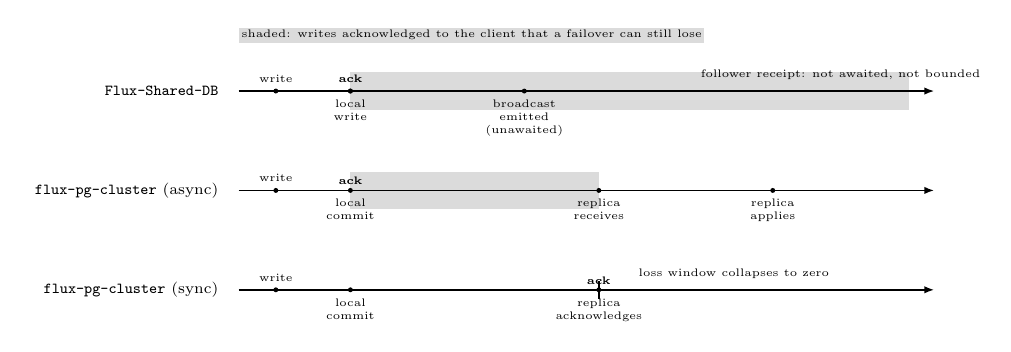
\begin{tikzpicture}[
  font=\scriptsize, x=1mm, y=1mm,
  ax/.style={-{Latex[length=1.6mm]}, thick},
  ev/.style={circle, fill=black, inner sep=0.8pt},
  lbl/.style={font=\tiny, align=center, inner sep=1pt},
  nm/.style={font=\scriptsize, anchor=east},
  loss/.style={fill=black!14},
]
  % ---- timeline 1: Flux-Shared-DB
  \fill[loss] (18,34) rectangle (108,40);
  \draw[ax] (0,37) -- (112,37);
  \node[nm] at (-2,37) {\texttt{Flux-Shared-DB}};
  \node[ev] (w1)  at (6,37)  {}; \node[lbl, above=0.5mm of w1] {write};
  \node[ev] (l1)  at (18,37) {}; \node[lbl, below=0.5mm of l1] {local\\write};
  \node[ev] (a1)  at (18,37) {}; \node[lbl, above=0.5mm of a1] {\textbf{ack}};
  \node[ev] (b1)  at (46,37) {}; \node[lbl, below=0.5mm of b1] {broadcast\\emitted\\(unawaited)};
  %% y=37.2 put this on the axis itself; the rule struck through the text.
  \node[lbl, anchor=west] at (74,39.6) {follower receipt: not awaited, not bounded};

  % ---- timeline 2: flux-pg-cluster, async
  \fill[loss] (18,18) rectangle (58,24);
  \draw[ax] (0,21) -- (112,21);
  \node[nm] at (-2,21) {\texttt{flux-\allowbreak{}pg-\allowbreak{}cluster} (async)};
  \node[ev] (w2)  at (6,21)  {}; \node[lbl, above=0.5mm of w2] {write};
  \node[ev] (c2)  at (18,21) {}; \node[lbl, below=0.5mm of c2] {local\\commit};
  \node[lbl, above=0.5mm] at (18,21) {\textbf{ack}};
  \node[ev] (r2)  at (58,21) {}; \node[lbl, below=0.5mm of r2] {replica\\receives};
  \node[ev] (p2)  at (86,21) {}; \node[lbl, below=0.5mm of p2] {replica\\applies};

  % ---- timeline 3: flux-pg-cluster, synchronous
  \draw[ax] (0,5) -- (112,5);
  \node[nm] at (-2,5) {\texttt{flux-\allowbreak{}pg-\allowbreak{}cluster} (sync)};
  \node[ev] (w3)  at (6,5)  {}; \node[lbl, above=0.5mm of w3] {write};
  \node[ev] (c3)  at (18,5) {}; \node[lbl, below=0.5mm of c3] {local\\commit};
  \node[ev] (r3)  at (58,5) {}; \node[lbl, below=0.5mm of r3] {replica\\acknowledges};
  \node[lbl, above=0.5mm] at (58,5) {\textbf{ack}};
  \draw[very thick] (58,3.6) -- (58,6.4);
  %% Same as the first timeline: 0.6 above a rule at y=5 still crosses the glyphs.
  \node[lbl, anchor=west] at (64,7.6) {loss window collapses to zero};

  \node[lbl, anchor=west, fill=black!14, inner sep=1.2pt] at (0,46)
    {shaded: writes acknowledged to the client that a failover can still lose};
\end{tikzpicture}

\caption{Write-acknowledgment timing relative to replication, compared across
\texttt{Flux-Shared-DB} and the two \texttt{flux-\allowbreak{}pg-\allowbreak{}cluster} replication modes.}
\label{fig:managed-db-ack-timing}
\end{figure}

\subsection{How a tenant uses these}
\label{subsec:managed-db-tenant}

\paragraph{\texttt{Flux-Shared-DB}.} A tenant registers two \FluxOS application
components --- a stock \texttt{mysql:latest}\slash\texttt{mariadb} engine and the
\texttt{runonflux/\allowbreak{}shared-\allowbreak{}db} Operator image --- or a single bundled image with the
engine baked in \srcdoc{Flux-Shared-DB/README.md:20-49,73-101}. Credentials are set at
first boot via \texttt{DB\_INIT\_PASS}\slash\texttt{DB\_USER} environment variables and are
not re-keyable afterward: ``changing it later will not re-key an already-initialized
\texttt{/app/db} datadir'' \srcdoc{Flux-Shared-DB/README.md:88}. The tenant application
connects with an ordinary MySQL connection string to the Operator's proxy port (default
3307) \srcdoc{Flux-Shared-DB/README.md:46-49}. As established in
\S\ref{subsec:flux-shared-db}, authorization at that proxy is IP-allowlist-based, not
credential-based, and internal cluster traffic (queries, keys, session tokens) is
plaintext Socket.IO by default, since the AES ``comm'' layer's key exchange is
commented out. The debug UI can optionally run over TLS with a self-signed certificate
if \texttt{SSL=true}, default \texttt{false}
\srccode{Flux-Shared-DB/\allowbreak{}ClusterOperator/\allowbreak{}Security.js}{163-185}
\srccode{Flux-Shared-DB/\allowbreak{}ClusterOperator/\allowbreak{}config.js}{25}. No at-rest encryption of the
MySQL/MariaDB data directory was found in the repository.

\paragraph{\texttt{flux-\allowbreak{}pg-\allowbreak{}cluster}.} A tenant registers a single \FluxOS application
component with a fixed port set (5432, 5433, 8008, 2379, 2380)
\srcdoc{flux-pg-cluster/README.md:78}. Superuser and replication credentials are
supplied as \texttt{POSTGRES\_SUPERUSER\_PASSWORD}\slash\texttt{POSTGRES\_REPLICATION\_PASSWORD}
environment variables and persisted, shell-quoted, to \texttt{/\allowbreak{}etc/\allowbreak{}cluster\_env} for
reuse by later agent subcommands
\srccode{flux-pg-cluster/\allowbreak{}internal/\allowbreak{}config/\allowbreak{}config.go}{331-332}. Tenants connect through
the primary-routing proxy on port 5433, which always routes writes to the current
primary across failovers, or bypass it to a specific node on 5432 for read-only access
to a replica \srcdoc{flux-pg-cluster/README.md:284-338}. Encryption is opt-in:
\texttt{SSL\_ENABLED} defaults to \texttt{false}
\srccode{flux-pg-cluster/\allowbreak{}internal/\allowbreak{}config/\allowbreak{}config.go}{117}; when set, a deterministic
self-signed CA and per-service TLS certificates are generated for PostgreSQL,
\texttt{etcd} peer/client traffic, and the Patroni REST API, and \texttt{pg\_hba}
accepts \texttt{hostssl}\slash\texttt{cert clientcert=verify-\allowbreak{}full} for replication
connections alongside plain \texttt{host} md5 entries that the template and the
reconciler retain in either mode \srccode{flux-pg-cluster/\allowbreak{}generate-certs.sh}{45-306}
\srccode{flux-pg-cluster/\allowbreak{}patroni.yml.tpl}{69-73}
\srccode{flux-pg-cluster/\allowbreak{}cmd/\allowbreak{}flux-agent/\allowbreak{}daemon.go}{452-457}. With \texttt{SSL\_ENABLED=\allowbreak{}false}, the
default, inter-node PostgreSQL replication and \texttt{etcd} traffic run over the
public internet in plaintext --- the project's own architecture documentation labels
this path ``Replication via Public Internet'' \srcdoc{flux-pg-cluster/README.md:55}.
As with \texttt{Flux-Shared-DB}, no at-rest encryption of the PostgreSQL data directory
was found in the repository.

\subsection{Backup and restore}
\label{subsec:managed-db-backup}

\paragraph{\texttt{Flux-Shared-DB}.} Backups are periodic full \texttt{mysqldump}
snapshots, taken as part of the log-compaction cycle described in the evidence,
written to \texttt{./dumps/*.sql} inside the container and retaining only the two most
recent files \srccode{Flux-Shared-DB/\allowbreak{}ClusterOperator/\allowbreak{}Operator.js}{504-548}. If the
application's declared container data includes \texttt{s:/app/dumps}, \FluxOS's own
directory-sync mechanism replicates that path across the app's instances --- this
sync is a \FluxOS-level feature, not code in the operator repository itself
\srcdoc{Flux-Shared-DB/README.md:76,81-83}. Anyone who can reach the debug UI and
authenticate via a Bitcoin-message-signature login tied to the application owner's
ZelID can list, download, or delete backups, or execute an uploaded or
URL-fetched \texttt{.sql} file directly into the live cluster via
\texttt{/executebackup}, which first rolls the database back to sequence zero --- i.e.,
wipes it --- before importing \srccode{Flux-Shared-DB/\allowbreak{}ClusterOperator/\allowbreak{}server.js}{653-715}.
No evidence of restore being exercised by an automated test was found; the only test
file in the repository covers signature verification, unrelated to backup or restore
\srccode{Flux-Shared-DB/\allowbreak{}test/\allowbreak{}bitcoinMessage.test.js}{1-18}.

\paragraph{\texttt{flux-\allowbreak{}pg-\allowbreak{}cluster}.} An opt-in (\texttt{BACKUP\_ENABLED=\allowbreak{}false} by
default \srcdoc{flux-pg-cluster/README.md:170}) backup agent runs \texttt{pg\_dumpall},
gzip-compresses the result, and overwrites a previous backup only after an integrity
check (valid gzip, and presence of the ``PostgreSQL database dump complete'' marker)
via a temp-file-then-atomic-rename pattern
\srccode{flux-pg-cluster/\allowbreak{}cmd/\allowbreak{}flux-agent/\allowbreak{}backup.go}{90-143,204-223}. Backups run only on
whichever node Patroni currently reports as the healthy running primary, avoiding
duplicate copies
\srccode{flux-pg-cluster/\allowbreak{}cmd/\allowbreak{}flux-agent/\allowbreak{}backup.go}{93-99,145-164}. Retention keeps the
newest \texttt{BACKUP\_RETENTION\_COUNT}$=1$ (default) files, then prunes further by a
total-size cap that is unlimited by default
\srccode{flux-pg-cluster/\allowbreak{}cmd/\allowbreak{}flux-agent/\allowbreak{}backup.go}{275-337}. Backup storage is
\texttt{/\allowbreak{}var/\allowbreak{}lib/\allowbreak{}postgresql/\allowbreak{}backups}, explicitly documented as \emph{not} covered by
persisting the main data-directory volume, and lost on reschedule unless separately
persisted \srcdoc{flux-pg-cluster/README.md:77,276}. Restore is a manual, documented
\texttt{gunzip~|~psql} command \srcdoc{flux-pg-cluster/README.md:280-282}; the README
itself instructs the operator to ``verify restores regularly'' as their own
responsibility \srcdoc{flux-pg-cluster/README.md:186}, which is a stronger honesty
signal than a silent absence of guidance but does not amount to an automated restore
guarantee. A file named \texttt{test\_restore\_reconciliation.\allowbreak{}py} exists in the same
test suite \srccode{flux-pg-cluster/\allowbreak{}tests/\allowbreak{}scenarios/\allowbreak{}}{test\_restore\_reconciliation.py},
but its contents were not reviewed for this section, so it is not counted here as
verified automated restore coverage.

For neither system, then, has restore been exercised in a way this section can verify
end to end: \texttt{Flux-Shared-DB} has no restore test at all, and
\texttt{flux-\allowbreak{}pg-\allowbreak{}cluster}'s restore path is documented as a manual operation with an
unreviewed test file of unknown scope.

\subsection{RPC, archive, and indexing (\planned)}
\label{subsec:rpc-archive-indexing}

The roadmap names RPC, archive, and indexing services the network's ``first
capacity-selling product,'' scheduled for Q3 2026
\srcroadmap{flux-roadmap-public.md:33-34}, and states that this product ``pairs
directly with chain pruning: the archive nodes pruning requires become the product''
\srcroadmap{flux-roadmap-public.md:34}. Main-chain pruning itself is treated at
reimplementation depth in \S8; the roadmap's own framing of pruning is that ``pruned
nodes stay fully able to produce blocks, with designated archive nodes preserving full
history for explorers and the data services above''
\srcroadmap{flux-roadmap-public.md:121-122}. The direction of dependency between the two
items is stated loosely (``pairs directly with''), not as a strict blocking gate
\srcinferred.

No RPC, archive, or indexing implementation was surveyed for this section: the evidence
available covers only the two managed-database operators above, and no repository
matching an RPC gateway, an archive-node service, or an indexing service was read. This
item is therefore reported here purely as a roadmap commitment, and its construction is
left explicitly open rather than described as a system that does not yet exist.
\begin{remark}[The shape of the RPC product --- settled at the architectural level]
\label{rem:rpc-shape}
The request-routing model was carried as undecided. Its architecture is now settled, and in a way
that answers the structural half of the question while leaving the commercial half open:
\textbf{archive nodes run as \FluxCloud{} applications}, deployed by the team, with access to RPC and
other node APIs sold as a product \srcintent{08-answers-round-2.md, round 16} (\planned).

That decides three things. Routing is to \emph{operator-deployed shared endpoints} rather than to
per-tenant archive deployments --- a tenant buys API access, not a node. The pruning-exempt storage
requirement does not interact with the tiering and collateral model of \S\ref{sec:consensus} at all,
because an archive node is a tenant workload subject to the application resource model, not a
\FluxNode{} tier: it needs no collateral and confers no eligibility. And history availability is
consequently a property of this product rather than of the node set
(\Cref{rem:archive-product}).

What remains commercial rather than architectural: the indexing schema and the pricing unit --- per
request, per method, per byte returned, or a flat subscription. Those do not constrain any mechanism
in this paper and are not stated here.
\end{remark}

Whatever this product becomes, it will inherit the same question this section has just
answered for the two managed-database implementations: what does the platform promise
about durability and consistency, and under what replication or storage protocol.
Archived chain history is, if anything, a harder case than a tenant's own database,
because it is by definition unrecoverable once lost from every archive node
simultaneously; the paper takes no position here on which of the two postures compared
above --- hand-rolled and untested, or consensus-backed and failure-tested --- an
archive service would follow, because no such service has been surveyed.

\subsection{Implication for lifecycle: eviction is where the guarantee is tested}
\label{subsec:managed-db-lifecycle}

The containers that implement both systems above are, from the node's point of view,
ordinary Docker containers, and they are stopped through the same generic pipeline as
any other application when a node evicts, redeploys, or is asked to stop an
application. In production today, that pipeline executes only its Signal and Cleanup
stages; the drain and pre-stop hook stages exist in the state machine and are
unit-tested, but are ``not yet reachable from real events''
\srccode{flux-shutdownd/\allowbreak{}crates/\allowbreak{}shutdownd/\allowbreak{}src/\allowbreak{}pipeline/\allowbreak{}state\_machine.rs}{3-7}, even
though the underlying mechanism already reads per-container
\texttt{shutdown.\{drain,prestop,graceful\}-s} labels intended to drive exactly this
behavior \srccode{flux-shutdownd/\allowbreak{}crates/\allowbreak{}shutdownd/\allowbreak{}src/\allowbreak{}config.rs}{41-65}. For a
stateless workload, skipping a drain step is a latency blip. For a managed database, it
is the difference between an orderly checkpoint and whatever durability guarantee ---
or absence of one --- \S\ref{subsec:managed-db-comparison} describes: an application
that is killed rather than quiesced is, from the perspective of
Property~\ref{prop:sharedb-durability}, indistinguishable from a crash.

This is the requirement §16 must carry forward: a managed database is a stateful
service whose eviction destroys data, so the grace, suspension, and eviction state
machine that governs how and when a node stops an application matters more here than
for any stateless workload this paper describes elsewhere.

%% Drain this section's float queue before the next begins.
\FloatBarrier

\section{Attested execution: \ArcaneOS, the \SAS, and the attestation network}
\label{sec:attested-execution}\label{sec:attestation}

A node that lies about its own hardware is one problem; a node that boots something other than
the image it claims to run is a different, sharper one. \ArcaneOS is Flux's answer to the second
problem: a hardened Linux image with measured boot, disk encryption tied to the host, and a
signed root filesystem, running a local service (\fluxsas, the \SAS) that other components query
before they trust a node. The chain from firmware to a locked-down running system does real,
verifiable work, and the update mechanism that ships new images is a carefully engineered,
deliberately centralized ceremony. What the resulting \emph{attestation} — the signed statement a
node can produce about itself — does not do is bind that statement to the specific machine that
produced it. This section describes the deployed chain first, states exactly where that binding
fails, and then specifies the bonded attestation network the roadmap proposes as the fix: an
approach that replaces "trust the key" with "trust the capital at risk," which is a primitive
Flux already has and a hardware root of trust is not.

\subsection{The deployed attestation stack}

\subsubsection{The boot chain}
\label{sec:boot-chain}

On a bare-metal or VPS install, \ArcaneOS's Secure Boot Platform Key (PK), Key Exchange Key (KEK)
and signature database (db) are written into the machine's live UEFI variables at install time
from \texttt{.auth} artifacts staged on the EFI system partition, replacing whatever keys were
present, after which the revocation database (dbx) is made immutable with \texttt{chattr~+i}
\shipped~\srccode{fluxos-iso/\allowbreak{}flux\_fs/\allowbreak{}fs\_scaffold/\allowbreak{}curtin/\allowbreak{}curtin-hooks}{26--43}. This is a
Flux-controlled Platform Key, not a hardware-vendor or Microsoft key: its SHA-256 hash is a
build-time constant (\texttt{FLUX\_PK\_SHA256SUM}) baked into the \texttt{fes} ("Flux Enrollment
Service") binary \shipped~\srccode{fluxos-iso/\allowbreak{}Makefile}{65}.

At boot, \texttt{fes} and \fluxsas independently re-derive that trust. \fluxsas's
\texttt{check\allowbreak{}Secure\allowbreak{}Boot()} reads the UEFI \texttt{SecureBoot} variable and calls a fatal
\texttt{terminateApp()} if Secure Boot is not enabled \shipped~\srccode{fluxsas/\allowbreak{}src/\allowbreak{}sas.cpp}{101--110}.
\texttt{fes} performs the identical check during first-boot enrollment and, on the initrd side,
\texttt{fes-wrapper} treats \texttt{fes}'s exit code as its entire contract: exit \texttt{50}
means Secure Boot is disabled, \texttt{51} means the enrolled Platform Key's hash did not match
the pinned value, \texttt{52} means no TPM2 device is present, and any other nonzero code is a
generic enrollment failure — on any of these, the initrd prints a warning to the console, waits
up to 30~seconds, and powers the machine off rather than continuing to boot
\shipped~\srccode{fluxos-iso-pkcs11/\allowbreak{}99flux-crypt/\allowbreak{}fes-wrapper}{1--45}. The fuller code set
(\texttt{53}--\texttt{57}, covering TPM2 enrollment failure, the VPS check, PKCS\#11 enrollment,
keystore failure and device-unlock failure) is defined alongside these in the same enrollment
tool \shipped~\srccode{fluxsas/\allowbreak{}secrets}{FES\_EXIT\_* block}. This is a real fail-closed boot gate,
correctly credited: a node that cannot prove Secure Boot is on, with the right key, and a TPM2
present, does not come up at all.

Where a TPM2 device exists, \texttt{fes} enrolls it against the system LVM volume with
\texttt{systemd-\allowbreak{}cryptenroll -\allowbreak{}-\allowbreak{}wipe-\allowbreak{}slot=all -\allowbreak{}-\allowbreak{}tpm2-\allowbreak{}device=auto -\allowbreak{}-\allowbreak{}tpm2-\allowbreak{}pcrs=7}
\shipped~\srccode{fluxsas/\allowbreak{}src/\allowbreak{}fes/\allowbreak{}fes.cpp}{173--186}. Only PCR~7 is sealed against — the PCR that
measures Secure Boot policy state (PK/KEK/db/dbx contents and the enabled flag), not the kernel,
initrd, or root filesystem image. The direct consequence, read from the enrollment code rather
than inferred, is that a TPM-sealed key unseals for \emph{any} kernel and initrd signed under the
pinned Platform Key, not specifically the build that was running when the key was sealed —
image-version binding is not something the TPM seal itself provides.

Root disk unlock is offered both hardware and software paths simultaneously:
\texttt{systemd-cryptsetup@root.\allowbreak{}service} attaches the root LUKS volume with
\texttt{tpm2-\allowbreak{}device=auto,pkcs11-\allowbreak{}uri=auto} set together
\shipped~\srccode{fluxos-iso-pkcs11/\allowbreak{}99flux-crypt/\allowbreak{}cryptsetup-wrapper}{5--7}. Where no TPM2 device
is present, \texttt{fes} first checks whether the host is a hosting/VPS IP via a third-party
lookup \shipped~\srccode{fluxsas/\allowbreak{}src/\allowbreak{}fes/\allowbreak{}fes.cpp}{205--236}, then falls back to a software PKCS\#11
token: an RSA-4096 key generated inside a SoftHSM2 store held in an encrypted loopback image
\shipped~\srccode{fluxsas/\allowbreak{}src/\allowbreak{}fes/\allowbreak{}fes.cpp}{102--141,244--276}, with a PIN derived from local machine values
and written in plaintext to \texttt{/\allowbreak{}etc/\allowbreak{}credstore/\allowbreak{}cryptsetup.\allowbreak{}pkcs11-pin} — a placement the source
comment itself flags as unresolved (\emph{"Move this to socket"})
\shipped~\srccode{fluxsas/\allowbreak{}src/\allowbreak{}fes/\allowbreak{}fes.cpp}{239--241,356}. \textbf{This fallback is where the
guarantee weakens}: the SoftHSM2 token database is protected at rest by a static key compiled into
every \fluxsas binary rather than by hardware, so per-machine sealing degrades to
per-machine-plus-anyone-who-reads-the-binary sealing. The fallback exists mainly for VPS hosts
that do not expose custom Secure Boot key enrollment to the guest, and the \ArcaneOS documentation
itself notes this population is shrinking as providers close that off
\srcdoc{fluxos-iso/README.md:289--296}.

Root filesystem integrity is enforced by dm-verity: \fluxsas parses \texttt{veritysetup status}
for the active root hash and its \texttt{verified} status
\shipped~\srccode{fluxsas/\allowbreak{}src/\allowbreak{}watchdog.h}{449--506}. This confirms the running rootfs is mounted
under dm-verity; the boot-time source of the \emph{expected} root hash consumed by the initrd is
not established by the evidence available for this section and is not asserted here. Finally, the
initrd mitigates the physical-access window between an unattended install and first boot: once a
disk-unlock token has been enrolled, \texttt{flux-\allowbreak{}init-\allowbreak{}cleanup} mounts the plaintext,
\texttt{root}-labelled filesystem and deletes everything on it except the current squashfs image,
its verity file, install logs, and small configuration files, specifically "to mitigate the
primary drive being mounted by an attacker after installation, but before first boot"
\shipped~\srccode{fluxos-iso-pkcs11/\allowbreak{}99flux-crypt/\allowbreak{}flux-init-cleanup}{20--60}. A real window remains
between install completion and that cleanup pass, during which the plaintext root and the
unencrypted EFI system partition are both mountable by anyone with physical access to the disk.

\subsubsection{The update channel}
\label{sec:update-channel}

The strongest link in the chain is how a new \ArcaneOS image reaches every node. Release signing
runs through a physically Flux-operated YubiHSM~2, whose objects include a dedicated Ed25519
release-signing key (\texttt{Flux\allowbreak{}Os\allowbreak{}Release\allowbreak{}Key}) alongside the Secure Boot signing keys
\shipped~\srccode{flux-iso-hsm/\allowbreak{}src/\allowbreak{}flux\_hsm/\allowbreak{}hsm\_manager.py}{178--544}. A human custodian
authenticates to the HSM with their own personal YubiKey via challenge-response key derivation, so
no raw password ever leaves the YubiKey \shipped~\srccode{flux-iso-hsm/\allowbreak{}src/\allowbreak{}flux\_hsm/\allowbreak{}hsm\_manager.py}{686--764},
and a build session's actual signing credentials are fresh, single-use authentication keys created
for that session and expected to be deleted afterward
\shipped~\srccode{flux-iso-hsm/\allowbreak{}src/\allowbreak{}flux\_hsm/\allowbreak{}hsm\_manager.py}{1064--1110}. The HSM's own master
wrap key is backed up by Shamir's Secret Sharing across an $M$-of-$N$ set of custodians, driven end
to end over a dedicated ceremony protocol
\shipped~\srccode{flux-iso-hsm/\allowbreak{}src/\allowbreak{}flux\_hsm/\allowbreak{}server/\allowbreak{}sss.py}{12--37}. A finished build is bundled
into a release tarball and signed with that Ed25519 key over a chunked SHA-256 digest of the whole
artifact \shipped~\srccode{fluxos-iso/\allowbreak{}flux-release-signer/\allowbreak{}src/\allowbreak{}flux\_release\_signer/\allowbreak{}main.py}{69--152};
every node verifies incoming updates against a single Ed25519 public key baked into the image at
build time \shipped~\srccode{fluxos-iso/\allowbreak{}flux\_fs/\allowbreak{}build\_target.sh}{81--84}.

Stated plainly: \textbf{only Flux can publish an \ArcaneOS update.} Every node verifies an incoming
update against exactly one embedded Ed25519 public key and no other
\shipped~\srccode{fluxos-iso/\allowbreak{}flux\_fs/\allowbreak{}build\_target.sh}{81--84}, and the only private key that
verifies against it lives inside the Flux-operated HSM behind the custodian ceremony described
above \shipped~\srccode{flux-iso-hsm/\allowbreak{}src/\allowbreak{}flux\_hsm/\allowbreak{}hsm\_manager.py}{336,1064--1110}; whoever holds
that HSM key can therefore produce an update every node's updater will accept. This is not an
oversight; the ceremony design — personal-YubiKey custodian authentication, single-use per-build
signing keys, and Shamir-split master-key recovery, all cited above — is a deliberate, carefully
engineered centralization of exactly one function. It should be read as such rather than
apologized for. (A WireGuard-tunneled fast path for the signing session exists alongside the
default SSH-tunneled one but is gated behind a flag documented as defaulting to off, and is tagged
\inprogress here rather than folded into the ceremony's shipped description
\srcdoc{flux-iso-hsm/docs/SETUP\_FLOW.md:333--353}.) The
one caveat worth stating alongside it: the same build scripts that produce production releases
also carry explicit debug bypasses (\texttt{SKIP\_RELEASE\_SIGNING}, \texttt{SKIP\_LIVE\_SIGNING})
that ship an unsigned tarball, UKI, or kernel module if set
\shipped~\srccode{fluxos-iso/\allowbreak{}build\_dist.sh}{101--114}
\srccode{fluxos-iso/\allowbreak{}flux\_fs/\allowbreak{}build\_kmss.sh}{50--53}
\srccode{fluxos-iso/\allowbreak{}live\_iso/\allowbreak{}build\_uki.sh}{47--48}; if either flag is set on a production
build, the signature chain for that artifact is void, and no code in these repositories checks
that a released artifact was actually signed before publication.

\subsubsection{The \fluxsas protocol}

\fluxsas serves a single listener at \texttt{https:/\allowbreak{}/\allowbreak{}127.\allowbreak{}0.\allowbreak{}0.\allowbreak{}1:16100}, bound to loopback, with
mutual TLS mandatory (\texttt{SSL\_VERIFY\_PEER\allowbreak\;|\;SSL\_VERIFY\_FAIL\_IF\_NO\_PEER\_CERT})
\shipped~\srccode{fluxsas/\allowbreak{}src/\allowbreak{}api\_server.h}{1042--1053,1020}. Authorization beyond the TLS
handshake is by client-certificate Common Name, checked once in a routing handler with no
per-route pinning at the TLS layer itself: the CN \fluxbench is authorized for every route
without exception, the CN \texttt{fdm-nginx} is authorized only for three routes
(\texttt{/v2/decrypt}, \texttt{/\allowbreak{}v2/\allowbreak{}ca\allowbreak{}Certificate}, \texttt{/v2/health}), and any other or missing
CN is rejected with HTTP~403 \shipped~\srccode{fluxsas/\allowbreak{}src/\allowbreak{}api\_server.h}{220--252}. Both
authorized callers are Flux-operated, node-local processes, not tenant-facing ones — a fact with
consequences below. Because \fluxbench carries blanket access, compromising it is
equivalent to compromising everything \fluxsas can sign, encrypt, or decrypt on that host, and
\fluxbench's own mTLS client identity toward \fluxsas is a hardcoded, network-wide Ed25519
keypair shipped in \fluxbench's source, not a per-node credential
\shipped~\srccode{fluxbench/\allowbreak{}src/\allowbreak{}fluxnode/\allowbreak{}sasclient.h}{73--99,80--84}.
The two checkouts read for this subsection do not interoperate: \fluxbench (\texttt{5504e5c},
2026-05-29) probes a plain-HTTP \texttt{localhost:\allowbreak{}16100} and sends its mTLS requests to
\texttt{https:/\allowbreak{}/\allowbreak{}localhost:16102}
\srccode{fluxbench/\allowbreak{}src/\allowbreak{}fluxnode/\allowbreak{}benchmarks.cpp}{4106}
\srccode{fluxbench/\allowbreak{}src/\allowbreak{}fluxnode/\allowbreak{}sasclient.h}{161,166}, while \fluxsas
(\texttt{711776d}, 2026-08-27) serves mTLS only, on 16100, and has no listener on 16102
\srccode{fluxsas/\allowbreak{}src/\allowbreak{}api\_server.h}{972--973,1046--1048}.
\notestablished{which \fluxbench and \fluxsas versions are paired on deployed nodes; the checkouts
read here are three months apart and incompatible as read, so the client behaviour in this
subsection is \fluxbench's and the listener behaviour is \fluxsas's, each at its own checkout.}

The route family of interest for attested execution is \texttt{/v2/attest} (Ed25519-signs a
caller-supplied message under a domain-separated key selected by a \texttt{purpose} argument —
absent, \texttt{cdn}, \texttt{mesh}, or \texttt{app}) and \texttt{/\allowbreak{}v2/\allowbreak{}attestationPublicKey} (returns
the corresponding public key) \shipped~\srccode{fluxsas/\allowbreak{}src/\allowbreak{}api\_server.h}{412--481,483--517}.
Adjacent routes cover a per-app transport key with its own domain-separated attestation
\shipped~\srccode{fluxsas/\allowbreak{}src/\allowbreak{}api\_server.h}{582--653} and a blob-upload signer
\shipped~\srccode{fluxsas/\allowbreak{}src/\allowbreak{}api\_server.h}{750--829}. Freshness is enforced unevenly: only the
\texttt{upload} and \texttt{manifest} kinds of \texttt{/\allowbreak{}v2/\allowbreak{}sign\allowbreak{}Blob\allowbreak{}Upload} check a $\pm300$-second
timestamp window at signing time \shipped~\srccode{fluxsas/\allowbreak{}src/\allowbreak{}api\_server.h}{183,780--829};
\texttt{/v2/attest} and \texttt{/\allowbreak{}v2/\allowbreak{}transportPublicKey} carry no server-enforced freshness at all,
so a verifier consuming either must supply its own staleness policy.

What a verifier learns from a successful \texttt{/v2/attest} call under \texttt{purpose=app} — the
route intended to bind a stored content hash to a validated envelope hash — is that some running
\fluxsas process produced a valid signature over that pair. Whether that constitutes evidence about
\emph{which} host produced it, and under what boot state, is exactly the question the next two
subsections answer.

\subsubsection{The trust root}

\begin{assumption}[The deployed attestation trust root]
\label{asm:trust-root}
The statement "this node booted something Flux considers legitimate" rests today on a compound
root that is entirely Flux-operated:
\begin{enumerate}
  \item a Flux-controlled UEFI Secure Boot Platform Key, pinned by hash inside the \texttt{fes}
  binary and checked against whatever key the firmware has enrolled
  \shipped~\srccode{fluxsas/\allowbreak{}src/\allowbreak{}fes/\allowbreak{}fes.cpp}{70--81};
  \item a Flux-operated pair of web services (\texttt{stats.\allowbreak{}runonflux.\allowbreak{}io} and
  \texttt{arcanehashes.\allowbreak{}app.\allowbreak{}runonflux.\allowbreak{}io}) that publish the set of dm-verity root hashes a node's
  watchdog treats as known-good, polled roughly once every 24--48 hours
  \shipped~\srccode{fluxsas/\allowbreak{}src/\allowbreak{}watchdog.h}{721--754}, and which \textbf{fail open}: if both
  endpoints are unreachable, the watchdog treats the running node as secure and takes no action
  \shipped~\srccode{fluxsas/\allowbreak{}src/\allowbreak{}watchdog.h}{566--596}; and
  \item a Flux-operated internal mTLS certificate authority that issues the client and server
  certificates every \fluxsas caller and listener presents.
\end{enumerate}
No independent hardware vendor, third-party attestation authority, or externally verified TPM
quote appears anywhere in this root.
\end{assumption}

None of this makes the boot chain worthless: measured boot, dm-verity, and LUKS unlock all impose
real, verifiable cost on a remote attacker with no local access. It does mean the assurance a node
offers is a Flux-operated one, not a hardware-rooted, independently verifiable one, and later
claims in this paper build on Assumption~\ref{asm:trust-root} exactly as stated, not on a stronger
reading of it.

\subsubsection{The property that does not hold}

\begin{property}[Attestation is not machine-bound]
\label{prop:not-machine-bound}
The Ed25519 signing key \texttt{/v2/attest} uses for the default, \texttt{cdn}, \texttt{mesh}, and
\texttt{app} purposes is derived by a key-derivation function from static values compiled
identically into every \fluxsas binary; none of the derivation's inputs depends on the TPM, on
Secure Boot state, or on any other per-machine value
\shipped~\srccode{fluxsas/\allowbreak{}src/\allowbreak{}api\_server.h}{411--481,466--469,503--506}. The one exception, the
node-identity key pair (\texttt{/\allowbreak{}v2/\allowbreak{}nodeIdentityPublicKey}, \texttt{/\allowbreak{}v2/\allowbreak{}nodeIdentitySign}), does
mix in a value derived from local machine identifiers, but the key that protects the random
component of that value at rest is itself a static value compiled into every binary
\shipped~\srccode{fluxsas/\allowbreak{}src/\allowbreak{}disk\_encryption.h}{200--228}. Consequently, a valid \fluxsas
attestation demonstrates possession of something every copy of the software contains — it does
not demonstrate that a particular machine booted a particular image. Compile-time obfuscation of
these constants changes what a casual binary scan reveals; it does not change this property.
\end{property}

This is stated as a property that fails, not as a procedure: no derivation input, salt, domain
value, or extraction path appears above or anywhere in this section, and none is needed to state
the property precisely. Property~\ref{prop:not-machine-bound} is the reason the bonded network
described in \S\ref{sec:bonded-network} exists, and it is the reason its Requirement~0 is written
the way it is.

\subsubsection{What a tenant can verify}
\label{sec:tenant-verify}

Today, nothing. Every \texttt{/v2/*} route on \fluxsas requires a client certificate issued by the
internal Flux mTLS CA and is reachable only on loopback
\shipped~\srccode{fluxsas/\allowbreak{}src/\allowbreak{}api\_server.h}{1042--1053,220--252}; an external tenant deploying an
application onto a \FluxOS node has no network path to \fluxsas at all, mTLS or otherwise. The
closest thing to a tenant-visible signal is the \texttt{purpose=app} attestation described above,
and no code path in the read repositories surfaces that signature to a tenant. Even if one did,
per Property~\ref{prop:not-machine-bound} it would prove "some \fluxsas process signed this," not
"this specific host booted a known-good image." There is no tenant-facing verification API, no
TPM-quote endpoint, and no remote-attestation client anywhere in \fluxsas or its provisioning
tooling.

\subsubsection{Residual trust surface}

Beyond the trust root of Assumption~\ref{asm:trust-root}, the deployed system asks a tenant to
accept the following, none of which \fluxsas measures or attests to:
\begin{itemize}
  \item \textbf{The container runtime.} Nothing in \fluxsas measures the Docker or Podman daemon;
  \texttt{are\allowbreak{}All\allowbreak{}Services\allowbreak{}Inactive()} checks that \texttt{containerd}, \texttt{docker.service}, and
  related units are \emph{inactive} before an unmount, which is a shutdown gate, not an integrity
  check \shipped~\srccode{fluxsas/\allowbreak{}src/\allowbreak{}disk\_encryption.h}{547--559,642}.
  \item \textbf{\FluxOS itself.} Application orchestration code runs outside \fluxsas's scope
  entirely; no file in the read evidence measures or attests to it.
  \item \textbf{Physical access.} Console access is explicitly exempted from the password-hash
  check applied to every other local account \shipped~\srccode{fluxsas/\allowbreak{}src/\allowbreak{}watchdog.h}{349--377},
  and the install-to-first-boot window described in \S\ref{sec:boot-chain} is a further,
  time-bounded physical exposure.
  \item \textbf{The update channel.} A single Flux-operated signing ceremony
  (\S\ref{sec:update-channel}) decides what code every node will accept as an upgrade; whoever
  holds that key can push code the entire fleet runs.
  \item \textbf{The hash allow-list service.} \texttt{stats.\allowbreak{}runonflux.\allowbreak{}io} and
  \texttt{arcanehashes.\allowbreak{}app.\allowbreak{}runonflux.\allowbreak{}io} decide what a running node considers a known-good image,
  fail open on outage, and are both Flux-operated.
  \item \textbf{The absence of a hypervisor boundary between tenants.} Application workloads run as
  containers directly on the \ArcaneOS host — the filesystem ships a
  \texttt{docker-to-podman-migration.\allowbreak{}service} unit, consistent with containers rather than
  per-tenant virtual machines as the isolation primitive on production nodes — and no evidence in
  the read repositories shows a per-tenant hypervisor-enforced boundary\srcinferred.
\end{itemize}

\subsection{The bonded attestation network}
\label{sec:bonded-network}

The roadmap's proposed fix would not be a better key; it would be a design that stops depending on
a key at all and depends on collateral instead. This subsection specifies a mechanism that does not
exist yet, and every claim in it is framed accordingly.

\begin{assumption}[Requirement 0]
\label{asm:requirement-zero}
A bonded attestation network would be meaningful only once two conditions hold that do not hold
today: the attestation signing key would need to be derived from, or sealed to, a per-machine
hardware root — TPM-sealed or Secure-Boot-bound, in a way Property~\ref{prop:not-machine-bound}
does not currently satisfy — and a tenant-reachable verification path would need to exist where
today there is none (\S\ref{sec:tenant-verify}). Absent the first condition, a bond would secure a
signature that anyone holding the \fluxsas software, not merely the bonded node, can produce today
(Property~\ref{prop:not-machine-bound}), which would make the bond forfeitable for statements the
bonded party never made. \srcintent{plan/mech-attestation-network.md, \S1}
\end{assumption}

\begin{construction}[The bonded network]
\label{cons:bonded-network}
A node $i$ would opt into the attested tier by posting a bond $\beta_i$ \emph{separate from} its
\FluxNode collateral. Base collateral would remain exactly as it is today — self-custodied,
refundable, untouched by any slashing path in this mechanism.

A \emph{claim} would be a tuple
$$
\mathsf{cl} = (\mathsf{subject}, \mathsf{predicate}, \mathsf{value}, \hgt, \mathsf{nonce}), \qquad
\sigma_{\mathsf{cl}} = \mathrm{Sign}_{sk_i}(H(\mathsf{cl})),
$$
where $\mathsf{subject}$ would name what is attested (an image digest, a reserve balance on a
foreign chain, a computation result, an observed state) and $\mathsf{predicate}$ would name the
assertion made about it. For each claim, a committee of $n$ bonded nodes would be sampled
deterministically from chain state,
$$
\mathcal{C}(\mathsf{cl}) = \mathrm{Top}_n\bigl(i \mapsto H(\mathsf{subject} \,\|\, \mathsf{prevHash}(\hgt) \,\|\, i)\bigr),
$$
reusing the sortition already implemented for \PoN slot eligibility in \fluxd — deterministic,
recomputable by any observer from chain state alone, and requiring no separate coordinator. A claim
would be \emph{accepted} once $k$ of the sampled $n$ nodes sign an identical $\mathsf{value}$,
\emph{disputed} if the committee splits, and \emph{challengeable} by any party for a window
$\Delta_{\mathrm{chal}}$ after acceptance. A challenger would post a bond $\beta_{\mathrm{chal}}$
alongside an assertion of the correct value; on a resolved challenge against the original signers,
each would be slashed by a fraction $s$ of $\beta_i$, and the challenger would be paid from the
slashed amount. A signer's bond would not be released while any claim it signed remains inside its
challenge window. \srcintent{plan/mech-attestation-network.md, \S2}
\end{construction}

Every slashing step above presumes that a bond can be forfeited on this chain at all, which
Bitcoin-derived script cannot express and which \Cref{op:slashing} leaves open.

\begin{openproblem}[Which claims a bond can actually secure]
\label{op:claim-classes}
The mechanism of Construction~\ref{cons:bonded-network} would be sound exactly over claims that are
\emph{objectively re-checkable}: an image digest, or a foreign-chain reserve balance at a stated
height, can be independently re-evaluated by any node, so a challenge would have an objective
resolution and slashing would be safe. "A computation the node ran," stated as a general claim
class, is not re-checkable in general — inputs may be gone, the computation may be
non-deterministic, or re-execution may itself be disputed — and slashing on a dispute with no
objective resolution would be a griefing vector against honest signers rather than a deterrent
against dishonest ones. The honest scope for a launch would be to restrict admissible claims to the
re-checkable class and leave general computation-integrity claims open until a resolution procedure
exists; this paper does not have one and does not invent one.
\srcintent{plan/mech-attestation-network.md, \S2.4} Reserve attestation for the
bridge (\S22) — the roadmap's own first customer for this mechanism — would fall inside the
re-checkable class, which is one reason to launch there first.
\proposednote{Re-checkable claims only at launch. A claim that cannot be re-evaluated has no
resolution procedure --- the dispute branch of \Cref{fig:challenge-protocol} terminates in nothing --- so
admitting one would mean accepting a bond that can never be adjudicated. Non-re-checkable classes can
be added once a resolution procedure exists for them; launching without that procedure would put the
mechanism's credibility on claims it cannot settle. \srcinferred.}
\end{openproblem}

A further constraint would be quantitative rather than procedural. For a reserve-attestation claim,
the gain from a successful false claim could be the entire balance being attested to, while the
cost of lying would be bounded by $s \cdot \beta_i$ times the probability of detection.
\textbf{A fixed bond cannot secure an unbounded reserve}: $\beta_i$ would need to scale with the
value being secured by the claims a node is sampled to sign, not with the node's \FluxNode
collateral tier, or the mechanism would be profitable to defeat exactly where it matters most — the
largest reserves.
\proposednote{$\beta_i$ is a function of value secured, not of tier: $\beta_i = \max(\beta_{\min},
\chi \cdot V_i)$ for value secured $V_i$, with $\chi$ the coverage ratio and $\beta_{\min}$ a floor
that keeps small claims worth adjudicating. Tier-based sizing is rejected because tier measures
collateral, not exposure --- a Cumulus node attesting a high-value claim would post less than a
Stratus node attesting a trivial one, which inverts the incentive. The coefficients $\chi$ and
$\beta_{\min}$ are calibration and are set with $(k,n)$ below. \srcinferred.} \proposednote{$n = \num{9}$, $k = \num{6}$, $\Delta_{\mathrm{chal}} = \num{2880}$ blocks
(\SI{24}{\hour}), slash fraction $s = 1$. Reasoning: $n=9$ keeps per-claim bandwidth and latency
modest while making a colluding majority expensive; $k/n = 2/3$ is the standard Byzantine threshold
and the smallest that tolerates $\lfloor (n-1)/3 \rfloor = 2$ faults; $\Delta_{\mathrm{chal}}$ of one
day gives a challenger a full business cycle to notice and act, and is the term $M \ge
\Delta_{\mathrm{chal}}$ in \S\ref{sec:chain-evolution} constrains. Full slashing rather than partial:
a partial slash prices dishonesty rather than deterring it, and the bond is already sized to the value
secured. \srcinferred.}

One seed of this mechanism already exists in the deployed system, \inprogress. The
\texttt{purpose=\allowbreak{}mesh} option on \texttt{/v2/attest} is described in \fluxsas's own source as "the
mesh membership voucher," with \FluxOS supplying \texttt{(mesh\allowbreak{}Ca, app\allowbreak{}Name, outpoint, recent block
hash)} as the payload for peers to verify against a mesh-purpose key
\srccode{fluxsas/\allowbreak{}src/\allowbreak{}api\_server.h}{438--445} — a node-to-node vouching primitive that is wired
into the API today with no caller anywhere in the read repositories that actually builds or checks
these vouchers. (The \FluxOS development fork's \texttt{wip/\allowbreak{}ingress-attestation} branch is
not a second seed: despite the name, the service it introduces attests the observed network source
of an \appspec submission, sealed to a team key and gossiped between nodes, and references \fluxsas
nowhere
\srcbranch{MorningLightMountain713/\allowbreak{}flux}{feat/fluxos-v9}{ZelBack/src/services/appMessaging/ingressAttestationService.js:1-40}.)
It is the
concrete starting point a bonded network would extend, not evidence that one exists.

\subsection{Figures}

\begin{figure}[H]
\centering
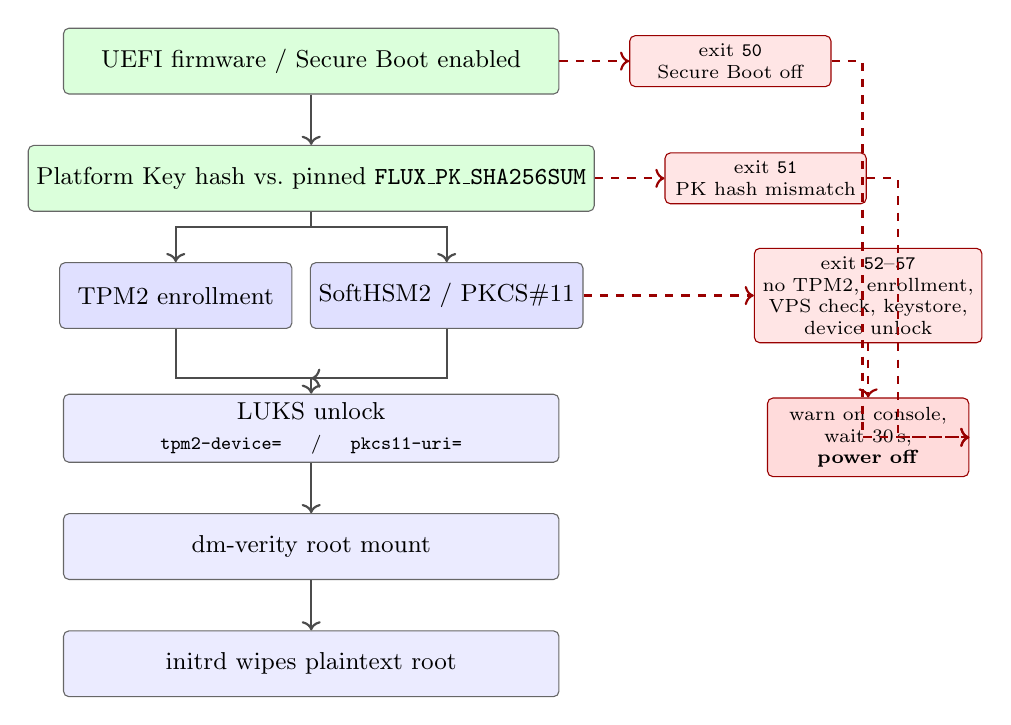
\begin{tikzpicture}[font=\small, node distance=6.5mm,
  stage/.style={draw=black!60, rounded corners=2pt, minimum width=6.4cm, minimum height=8.5mm,
                align=center, fill=blue!8, inner sep=3pt},
  gate/.style={stage, fill=green!14},
  br/.style={stage, fill=blue!12, minimum width=3.0cm},
  fail/.style={draw=red!60!black, fill=red!10, rounded corners=2pt, align=center,
               font=\scriptsize, inner sep=3pt, minimum width=2.6cm},
  ar/.style={->, thick, black!70},
  fa/.style={->, thick, red!60!black, dashed},
]
\node[gate] (sb) {UEFI firmware / Secure Boot enabled};
\node[gate, below=of sb] (pk) {Platform Key hash vs.\ pinned \texttt{FLUX\_PK\_SHA256SUM}};
\node[br, below=of pk, xshift=-1.75cm] (tpm) {TPM2 enrollment};
\node[br, below=of pk, xshift= 1.75cm] (p11) {SoftHSM2 / PKCS\#11};
\node[stage, below=8.5mm of pk, yshift=-1.5cm] (luks) {LUKS unlock \\ {\scriptsize\texttt{tpm2-device=\allowbreak{}} \quad / \quad \texttt{pkcs11-uri=}}};
\node[stage, below=of luks] (verity) {dm-verity root mount};
\node[stage, below=of verity] (wipe) {initrd wipes plaintext root};

\draw[ar] (sb) -- (pk);
\draw[ar] (pk.south) -- ++(0,-2mm) -| (tpm.north);
\draw[ar] (pk.south) -- ++(0,-2mm) -| (p11.north);
\draw[ar] (tpm.south) |- ($(luks.north)+(0,2mm)$) -- (luks.north);
\draw[ar] (p11.south) |- ($(luks.north)+(0,2mm)$);
\draw[ar] (luks) -- (verity);
\draw[ar] (verity) -- (wipe);

\node[fail, right=9mm of sb]  (f50) {exit \texttt{50}\\Secure Boot off};
\node[fail, right=9mm of pk]  (f51) {exit \texttt{51}\\PK hash mismatch};
\node[fail, right=22mm of p11] (f52) {exit \texttt{52}--\texttt{57}\\no TPM2, enrollment,\\VPS check, keystore,\\device unlock};
\draw[fa] (sb.east) -- (f50.west);
\draw[fa] (pk.east) -- (f51.west);
\draw[fa] (p11.east) -- (f52.west);

\node[draw=red!60!black, fill=red!14, rounded corners=2pt, below=7mm of f52,
      align=center, font=\scriptsize, minimum width=2.6cm] (off)
      {warn on console,\\wait \SI{30}{\second},\\\textbf{power off}};
\draw[fa] (f50.east) -- ++(4mm,0) |- (off.east);
\draw[fa] (f51.east) -- ++(4mm,0) |- (off.east);
\draw[fa] (f52) -- (off);
\end{tikzpicture}
\caption{The \ArcaneOS boot chain from firmware to a running, verity-protected root filesystem.}
\label{fig:boot-chain}
\end{figure}
%% Drafting note, not prose: the figure must show which stages terminate the boot on failure (Secure Boot, Platform Key,
%% TPM2 presence) versus which stages only degrade the guarantee (the SoftHSM2 fallback branch).

\begin{figure}[H]
\centering
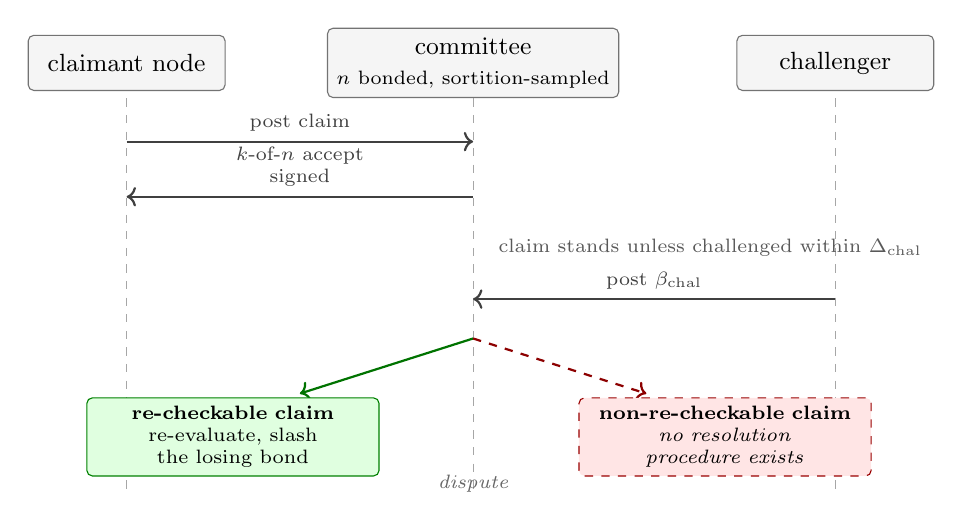
\begin{tikzpicture}[font=\small,
  life/.style={draw=black!55, fill=black!4, rounded corners=2pt, minimum width=2.5cm,
               minimum height=7mm, align=center, font=\small},
  msg/.style={->, thick, black!75},
  ok/.style={draw=green!50!black, fill=green!12, rounded corners=2pt, align=center,
             font=\scriptsize, inner sep=3pt, text width=3.5cm},
  open/.style={draw=red!60!black, fill=red!10, rounded corners=2pt, align=center,
               font=\scriptsize, inner sep=3pt, text width=3.5cm, dashed},
]
\node[life] (cl) at (0,0)  {claimant node};
\node[life] (cm) at (4.4,0) {committee\\{\scriptsize $n$ bonded, sortition-sampled}};
\node[life] (ch) at (9.0,0) {challenger};
\foreach \x in {0,4.4,9.0} \draw[black!35, dashed] (\x,-0.45) -- (\x,-5.5);

\draw[msg] (0,-1.0) -- node[above, font=\scriptsize] {post claim} (4.4,-1.0);
\draw[msg] (4.4,-1.7) -- node[above, font=\scriptsize, align=center]
  {$k$-of-$n$ accept\\{\scriptsize signed}} (0,-1.7);
\node[font=\scriptsize, text=black!65, anchor=west] at (4.6,-2.35)
  {claim stands unless challenged within $\Delta_{\mathrm{chal}}$};
\draw[msg] (9.0,-3.0) -- node[above, font=\scriptsize] {post $\beta_{\mathrm{chal}}$} (4.4,-3.0);

% divergence
\draw[->, thick, green!45!black] (4.4,-3.5) -- ++(-2.2,-0.7);
\draw[->, thick, red!55!black, dashed] (4.4,-3.5) -- ++(2.2,-0.7);
\node[ok]   at (1.35,-4.75) {\textbf{re-checkable claim}\\re-evaluate, slash the losing bond};
\node[open] at (7.6,-4.75) {\textbf{non-re-checkable claim}\\\textit{no resolution procedure exists}};
\node[font=\scriptsize\itshape, text=black!60] at (4.4,-5.35) {dispute};
\end{tikzpicture}
\caption{The bonded-network challenge protocol, showing where the mechanism's soundness depends on
the claim class.}
\label{fig:challenge-protocol}
\end{figure}
%% Drafting note, not prose: the figure must make the divergence between re-checkable and non-re-checkable claim
%% resolution visually explicit, since that divergence is Open Problem~\ref{op:claim-classes}, not a
%% detail.

%% Drain this section's float queue before the next begins.
\FloatBarrier


\fluxpart{Part IV}{Agents and value}
\section{Accelerated compute: GPUs and the AI workload path}
\label{sec:accelerated-compute}

An accelerator is not a fungible resource the way a CPU core or a gigabyte of RAM is: a GPU is
either present on a physical host or it is not, and whatever isolates one tenant's use of it from
another's is either enforced by the device driver and the orchestrator or it is not enforced at
all. This section asks two narrow questions about what \Flux actually ships today. First, what does
``pluggable GPU'' mean in code — is a GPU attached to a workload as a whole device, a slice of a
device, or something attachable and detachable at runtime? Second, what is the isolation boundary
between two tenants placed on the same machine? The answers are more restrictive than the roadmap's
language suggests, and one of the mechanisms below has a correctness defect worth stating plainly
rather than filing as a performance footnote. The evidence surveyed spans four repositories:
\texttt{fluxai} and \texttt{fluxai-\allowbreak{}enterprise} (an inference-as-a-service product), \texttt{pouwbackend}
(the \FluxEdge compute-rental marketplace), and \texttt{fluxai-\allowbreak{}fluxedge} (the GitOps glue between the
first two).

\subsection{GPU allocation as implemented}
\label{sec:accelerated-compute-allocation}

On the \FluxEdge marketplace, a rented workload's container requests a GPU the same way any
Kubernetes workload does: a resource quantity under the vendor device-plugin key \texttt{nvidia.com/gpu}
in the pod's \texttt{resources.\allowbreak{}limits}\slash\texttt{requests} \shipped\ \srccode{pouwbackend/\allowbreak{}rancher/\allowbreak{}deployment.go}{2155-2163}.
\texttt{set\allowbreak{}Resource\allowbreak{}Limit} reconciles the requested GPU \emph{count} against the rented computer's
actual GPU inventory, walking a bus-indexed enumeration of the machine's physical devices
(\texttt{newGPUIndexer}, NVIDIA-relative indexing) and appending each chosen bus index to the set of
GPUs already consumed by earlier containers of the same deployment \shipped\ \srccode{pouwbackend/\allowbreak{}rancher/\allowbreak{}deployment.go}{914-982},
\srccode{pouwbackend/\allowbreak{}rancher/\allowbreak{}deployment.go}{1245-1270}. Isolation between deployments sharing a rented
computer --- which on \FluxEdge belong to one renter, since a computer is rented exclusively
\srccode{pouwbackend/\allowbreak{}models/\allowbreak{}market\_place.sql.go}{1182-1190} --- is
then a single mechanism: the chosen bus indices are written into the container's
\texttt{NVIDIA\_VISIBLE\_DEVICES} environment variable \shipped\ \srccode{pouwbackend/\allowbreak{}rancher/\allowbreak{}deployment.go}{967-971}.
There is no further Flux-specific sandboxing layered on top of this; the isolation guarantee is
whatever the Kubernetes NVIDIA device plugin and the container runtime provide for an
environment-variable-scoped device list.

No time-slicing, no NVIDIA Multi-Instance GPU (MIG) partitioning, and no virtual-GPU (vGPU)
mechanism exists anywhere in the four repositories surveyed \shipped\ \srccode{pouwbackend/\allowbreak{}rancher/\allowbreak{}deployment.go}{914-982}.
This is a coherent design choice, not an oversight: whole-device passthrough with
environment-variable isolation is simple to reason about and gives strong isolation — a device
cannot be double-assigned across pods on the same node, because the device plugin never advertises
more \texttt{nvidia.com/gpu} resources than there are physical devices. The consequence is equally
direct: the granularity of what can be sold is fixed at one physical GPU. \FluxEdge cannot today
offer a fractional share of a GPU to two tenants concurrently; the only way to approximate a smaller
unit of accelerated compute is to dedicate an entire device to one renter and price accordingly.

\subsection{The contention defect: a resource request that disappears}
\label{sec:accelerated-compute-contention}

If none of a container's requested GPUs can be assigned --- the computer reports no NVIDIA
device, or every device is already taken by an earlier container of the same deployment ---
\texttt{set\allowbreak{}Resource\allowbreak{}Limit} does not reject the request and does not queue it for a computer with
sufficient capacity. It deletes the \texttt{nvidia.com/gpu} key from both \texttt{Limits} and
\texttt{Requests} on the container spec entirely \shipped\ \srccode{pouwbackend/\allowbreak{}rancher/\allowbreak{}deployment.go}{972-975}.
The workload is then scheduled and runs CPU-only, with no accelerator, and with no error surfaced to
the caller from this code path; the only trace is a log line from a failed resource-consumption
write, which is itself only logged rather than propagated \shipped\ \srccode{pouwbackend/\allowbreak{}rancher/\allowbreak{}deployment.go}{978-980}.
If only some of the requested GPUs can be assigned, the container receives that subset in
\texttt{NVIDIA\_VISIBLE\_DEVICES} while its declared limit is left unchanged, again with no error
\shipped\ \srccode{pouwbackend/\allowbreak{}rancher/\allowbreak{}deployment.go}{950-968}.

This is a correctness defect, not a performance characteristic. A caller who pays for and requests a
GPU-bearing deployment can receive a deployment silently missing the one resource that made the
request meaningful, and nothing in the API response distinguishes that outcome from a fully
provisioned rental. The correct behaviour, on contention, is to reject the rental request outright
or to queue it until a matching computer becomes available — either choice preserves the invariant
that a caller can trust an accepted request to mean what it says. Silently stripping the resource
line instead breaks that invariant in a way a paper describing this system should not pass over.

\subsection{``Pluggable'' or hot-attachable GPU: no code, no exception}
\label{sec:accelerated-compute-pluggable}

The roadmap's language of a ``pluggable'' or hot-attachable GPU has no counterpart in any of the
four repositories surveyed \srcdoc{plan/conflicts.md, C23}. An exhaustive search across all four
repositories for hot-attach, hot-plug, hot-swap, and pluggable terminology returns exactly one hit
outside vendor code, and it is unrelated: a \texttt{HotSwap} boolean field on OVH's public cloud
catalog API describing disk RAID hot-swap on dedicated servers, not GPU attachment
\srccode{pouwbackend/\allowbreak{}premium/\allowbreak{}ovh/\allowbreak{}ovh.go}{320}. There is no code anywhere in \texttt{fluxai},
\texttt{fluxai-\allowbreak{}enterprise}, \texttt{fluxai-\allowbreak{}fluxedge}, or \texttt{pouwbackend} that attaches a GPU to
an already-running container, or that reallocates a GPU between tenants without a pod
restart or reschedule. This is tagged \vision: it names a capability the roadmap gestures toward
that does not exist in code today, and the paper does not speculate about what a future
implementation might look like beyond that.

\subsection{Two product surfaces, easy to conflate}
\label{sec:accelerated-compute-surfaces}

The corpus contains two separate GPU-bearing product surfaces, and describing either as if it were
the other would misstate the system.

\texttt{fluxai} and \texttt{fluxai-\allowbreak{}enterprise} are an inference-as-a-service product — chat
completions, image generation, document intelligence — backed by a fixed, admin-provisioned pool of
GPU servers internally called ``RGP'' (Remote GPU). An administrator creates an RGP record, selects a
model, and triggers an asynchronous Ansible playbook that connects over SSH and stands up the
inference stack on the target rig \shipped\ \srccode{fluxai/\allowbreak{}fluxai\_admin/\allowbreak{}pages/\allowbreak{}views\_rgp.py}{36,468}.
There is no self-service provisioning path for an external caller in this product; capacity changes
only through this admin workflow, and \texttt{fluxai} is itself a tenant application deployed onto
\FluxCloud rather than part of the cloud substrate.

\texttt{pouwbackend} is the backend of \FluxEdge, a separate, Rancher/Kubernetes-orchestrated
compute-rental marketplace with its own OpenAPI-documented REST interface and its own CLI
\shipped\ \srccode{pouwbackend/\allowbreak{}rest\_api/\allowbreak{}v1/\allowbreak{}openapi.yaml}{1-4}. This is the mechanism described in
\S\ref{sec:accelerated-compute-allocation}--\S\ref{sec:accelerated-compute-contention}.

\texttt{fluxai-\allowbreak{}fluxedge} is the GitOps glue between the two: a repository of Kubernetes manifests and
Argo \texttt{Workflow} templates that clone the repository, build a \texttt{kustomize} overlay for a
given model, and \texttt{kubectl apply} it onto a node selected at submission time by \FluxEdge
\shipped\ \srccode{fluxai-fluxedge/\allowbreak{}custom-workflow-fluxone.yaml}{7-9,21-52}. In other words,
\texttt{fluxai}'s own inference pods are themselves provisioned as workloads on \FluxEdge — the two
product surfaces are physically coupled by self-hosting even though their APIs are independent
products, and a reader should not assume that describing one describes the other.

\begin{figure}[H]
\centering
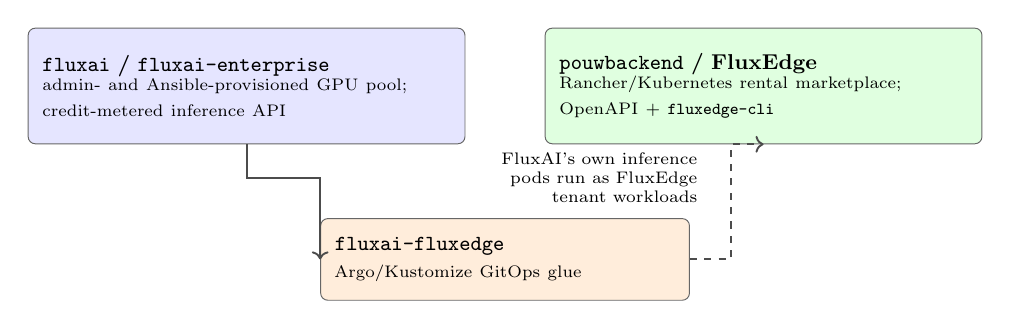
\begin{tikzpicture}[font=\small,
  b/.style={draw=black!60, rounded corners=3pt, align=left, inner sep=6pt, text width=6.0cm,
            minimum height=1.7cm},
  ai/.style ={b, fill=blue!10},
  edge/.style={b, fill=green!12},
  glue/.style={b, fill=orange!14, text width=5.0cm, minimum height=1.2cm},
]
\node[ai]   (ai)   at (0,3.1)  {\textbf{\texttt{fluxai} / \texttt{fluxai-\allowbreak{}enterprise}}\\
  {\scriptsize admin- and Ansible-provisioned GPU pool;\\credit-metered inference API}};
\node[edge] (fe)   at (7.6,3.1) {\textbf{\texttt{pouwbackend} / \FluxEdge{}}\\
  {\scriptsize Rancher/Kubernetes rental marketplace;\\OpenAPI ${+}$ \texttt{fluxedge-cli}}};
\node[glue] (glue) at (3.8,0.55) {\textbf{\texttt{fluxai-\allowbreak{}fluxedge}}\\
  {\scriptsize Argo/Kustomize GitOps glue}};

\draw[->, thick, black!70] (ai.south) -- ++(0,-0.5) -| (glue.west);
\draw[->, thick, dashed, black!70] (glue.east) -- ++(0.6,0) |- (fe.south);
%% Standalone, in the gap between the two boxes: on the edge at pos=0.72 it
%% printed on top of the pouwbackend/FluxEdge box.
\node[font=\scriptsize, text width=3.3cm, align=right, anchor=east] at (6.75,1.75)
  {FluxAI's own inference pods run as \FluxEdge{} tenant workloads};
\end{tikzpicture}
\caption{The two GPU-bearing product surfaces and the self-hosting relationship between them.}
\label{fig:accelerated-compute-surfaces}
\end{figure}

\subsection{A module name that is not a mechanism}
\label{sec:accelerated-compute-pouw}

\texttt{pouwbackend} is a mature compute-rental marketplace, and the paper describes it as exactly
that. Despite the name, ``Proof of Useful Work'' is not a designed consensus or verification
mechanism anywhere in this code. The only in-code hits for the term are a GPU mining-overclock
preset applied to a rig when its rental ends \shipped\ \srccode{pouwbackend/\allowbreak{}grpc\_server/\allowbreak{}market\_place/\allowbreak{}computer.go}{502,517},
and a Postgres schema documentation file that self-describes the database as the ``flux Prove Of
Useful Work Database (POUW)'' — branding, not a mechanism \shipped\ \srccode{pouwbackend/\allowbreak{}sql/\allowbreak{}.tbls.yml}{3}.
There is no submit-work, verify-work, or reward-work RPC triple; no on-chain anchoring of compute
results; and no linkage of any kind to \fluxd consensus. ``PoUW'' survives in this codebase only as a
Go module path and a database nickname. The paper does not describe \Flux as having a
proof-of-useful-work mechanism anywhere, and this section is where that is stated once, plainly, for
the record.

\subsection{The machine-facing surface: scoped tokens, forward to \S18}
\label{sec:accelerated-compute-machine-facing}

The \FluxEdge REST interface — OpenAPI 3.1.1, base path \texttt{/api/v1} — and its accompanying CLI,
\texttt{fluxedge-cli}, are the machine-facing surface this paper's agent-provisioning discussion in
\S18 depends on, not the fixed-credit inference API described above \shipped\ \srccode{pouwbackend/\allowbreak{}rest\_api/\allowbreak{}v1/\allowbreak{}openapi.yaml}{1-4}.
Authentication is by bearer token, and a key's privileges are enumerated rather than all-or-nothing:
\texttt{start\_rental}, \texttt{stop\_rental}, \texttt{start\_deployment}, \texttt{stop\_deployment},
and \texttt{get\_balance} \shipped\ \srccode{pouwbackend/\allowbreak{}rest\_api/\allowbreak{}v1/\allowbreak{}openapi.yaml}{2576-2581},
enforced in code by mapping each rental and deployment endpoint path to its required privilege
string --- the balance privilege is documented but has no entry in that map
\shipped\ \srccode{pouwbackend/\allowbreak{}rest\_api/\allowbreak{}ratelimit.go}{375-390}. Requests are rate-limited to two per
second per key and two per second per source IP \shipped\ \srccode{pouwbackend/\allowbreak{}rest\_api/\allowbreak{}ratelimit.go}{41-42};
a key or IP that accumulates five rate-limit violations within a five-minute window is automatically
revoked, its owner notified by email, and its cache entry evicted \shipped\ \srccode{pouwbackend/\allowbreak{}rest\_api/\allowbreak{}ratelimit.go}{43-45,203-222}.
This is a bounded, revocable \emph{action} authority — a human operator can mint a key that may start
rentals but not stop them, for example — suitable for handing to an autonomous agent with a defined
blast radius. No MCP server and no Terraform provider exist in any of these four repositories; the
MCP tools that do exist in the \Flux stack live elsewhere and are outside this section's scope, taken
up in \S18.

\subsection{Metering and the overdraft window, forward to \S16}
\label{sec:accelerated-compute-metering}

\texttt{fluxai}'s credit metering is asynchronous and eventually consistent rather than synchronous.
Each request is gated on a positive credit balance at call time, but usage is not deducted
immediately: token consumption accumulates in a Redis cache keyed per user with a 300-second expiry
\shipped\ \srccode{fluxai/\allowbreak{}api/\allowbreak{}cache.py}{9-32}, and a separate scheduled command later scans the
accumulated keys, applies the deduction to the persisted balance inside a locked transaction, and
clears the cache \shipped\ \srccode{fluxai/\allowbreak{}api/\allowbreak{}management/\allowbreak{}commands/\allowbreak{}process\_token\_usage.py}{41-99}.
The 300-second cache window is a real overdraft bound: a caller can spend up to that much usage
before the persisted balance reflects it, and the periodic flush job that closes the window is
itself scheduled through a live database-configured dispatcher rather than a fixed interval fixed in
source \shipped\ \srccode{fluxai/\allowbreak{}setup/\allowbreak{}crons/\allowbreak{}django\_cron}{2}. Any future product that prices
consumption rather than a subscription tier inherits this same window unless it is metered
differently; \S16's discussion of billing accuracy should carry this bound forward rather than
assume synchronous debiting.

\subsection{A gap for agent autonomy: key issuance}
\label{sec:accelerated-compute-key-issuance}

Nothing in \S\ref{sec:accelerated-compute-machine-facing} solves the problem of an agent obtaining
its own credential in the first place. API-key issuance is not exposed anywhere in the documented
REST v1 surface — only consumption is. The API's own quick-start documentation points a caller to the web
dashboard to obtain a key \shipped\ \srccode{pouwbackend/\allowbreak{}rest\_api/\allowbreak{}v1/\allowbreak{}openapi.yaml}{61}. A human must
mint a scoped key through that dashboard before an agent can use the \FluxEdge API autonomously; there
is no REST or CLI self-service path for an agent to request or rotate its own credential. This gap
is exactly the boundary \S17 and \S18 need to address for a fully autonomous provisioning workflow.

\subsection{Natural-language deployment: \texttt{DeploymentYAML}, forward to \S19}
\label{sec:accelerated-compute-nl-deploy}

\texttt{pouwbackend} exposes a gRPC method, \texttt{DeploymentYAML}, that generates Kubernetes YAML
from a natural-language prompt \shipped\ \srccode{pouwbackend/\allowbreak{}grpc\_server/\allowbreak{}market\_place/\allowbreak{}deployment.go}{1784-1812}.
The generation pipeline first performs a vector search over existing marketplace application YAMLs
to build retrieval-augmented context \shipped\ \srccode{pouwbackend/\allowbreak{}ai/\allowbreak{}fluxai.go}{188-191,241-244},
then dispatches a chat-completion request against a pinned model (``Llama 3.1 8B'') or, depending on
configuration, a third-party provider \shipped\ \srccode{pouwbackend/\allowbreak{}ai/\allowbreak{}fluxai.go}{212,266}. This is
the strongest existing evidence in the surveyed corpus for agent-native provisioning: a natural-language
deployment path is not a hypothetical for a future release, a form of it already ships. It is also,
for that reason, the concrete artifact \S19 should hold up when it takes up the question of whether a
generated specification is reviewable before it is signed and run.

\subsection{Resource accounting on the FluxOS side}
\label{sec:accelerated-compute-fluxos}

On the orchestration side, \FluxOS's per-tier resource allowances and its per-application hardware
check both express only the resource vector $\resvec = (\mathrm{cpu}, \mathrm{ram}, \mathrm{hdd})$:
the Cumulus/Nimbus/Stratus tier table gives total and application-available CPU (in tenths of a
core), RAM, and HDD per tier \shipped\ \srccode{flux/\allowbreak{}ZelBack/\allowbreak{}config/\allowbreak{}default.js}{380-403}, and the
per-application admission check (\texttt{check\allowbreak{}App\allowbreak{}HWRequirements}) validates a candidate application
against exactly those three dimensions \shipped\ \srccode{flux/\allowbreak{}ZelBack/\allowbreak{}src/\allowbreak{}services/\allowbreak{}appRequirements/\allowbreak{}hwRequirements.js}{370-408}.
No GPU resource class appears anywhere in this accounting. The v9 application specification (\S10)
adds a \texttt{machineType} enum with values \texttt{standard}, \texttt{gpu}, and \texttt{vps},
which is the field the specification intends to eventually carry a GPU-bearing workload declaration
\inprogress\ \srcbranch{flux}{feat/appspec-v9}{ZelBack/src/services/appRequirements/schemas/v9.json}.
As \S10 establishes, this field currently has no consumer code anywhere in \FluxOS
\srcdoc{plan/conflicts.md, C4}: it is declared in the schema and gated behind a feature flag that
nothing in the codebase flips, not wired to any placement, pricing, or admission logic.

\subsection{The workload class the substrate fits}
\label{sec:ac-workload-fit}

The preceding subsections describe what the accelerated-compute path can and cannot do. This one makes
an architectural claim about \emph{which kind of inference workload the network is structurally suited
to}, because the answer is not the one a reader primed by the frontier-model discourse would guess, and
because it bears directly on the thesis in \S\ref{sec:introduction}.

\paragraph{Why frontier inference centralises, and why that reason does not generalise.}
Serving a frontier model is not a single-device workload. Weights that exceed one accelerator's memory
are split across many, by tensor or pipeline parallelism, and every token generated requires
synchronous exchange between those devices. The interconnect carrying that exchange --- NVLink within
a chassis, InfiniBand across a rack --- is one to two orders of magnitude faster than commodity
wide-area networking, and the workload is latency-bound on it. This is why frontier inference
concentrates in single datacentres: it is a topology constraint, not a commercial preference, and no
amount of geographic distribution can be traded against it.

\begin{property}[The interconnect requirement is workload-specific]
\label{prop:ac-interconnect}
\srcinferred{} A model whose weights fit on one accelerator, or in host memory, requires no inter-device
communication during inference. Requests to such a model are mutually independent: there is no
synchronisation between concurrent users, and no state shared across nodes between requests.
Consequently the parallel efficiency of serving $n$ concurrent users across $n$ dispersed single-device
nodes is, to first order, the same as serving them from $n$ co-located devices.
\end{property}

\noindent The consequence is the section's substantive point. \textbf{For the workload class that fits
on one device, the structural advantage of centralisation disappears}, because the property that
creates it --- the interconnect --- is not exercised. A geographically dispersed, heterogeneous,
commodity fleet is not a compromised version of a datacentre for this class of work; it is an
appropriate substrate for it, and it brings two properties a datacentre does not: physical proximity to
the user, and per-tenant isolation that is a whole machine rather than a scheduler abstraction
(\S\ref{sec:accelerated-compute-allocation}).

\paragraph{What the network measurably has for it.}
Small quantised models are frequently served acceptably on CPU and host memory alone, with no
accelerator involved. The fleet's committed capacity is \num{8972} vCPU and \qty{17133.0}{\gibi\byte}
of RAM across \num{6489} nodes \srcmeasured{api.runonflux.io/\allowbreak{}apps/\allowbreak{}globalappsspecifications and
/\allowbreak{}daemon/\allowbreak{}getzelnodecount}{2026-09-03}, and that is capacity already committed to applications rather than
the fleet's ceiling. This is the part of the argument that needs no new engineering at all: the
CPU-served portion of this workload class is deployable on the substrate as it stands today, through the
ordinary application path of \S\ref{sec:fluxos}.

\paragraph{The tension, which is the honest half.}
\Flux's GPU allocation is whole-device passthrough, with no MIG partitioning, no vGPU and no
time-slicing anywhere in the surveyed code (\S\ref{sec:accelerated-compute-allocation}). \textbf{That is precisely the
wrong granularity for the workload this subsection argues the network suits.} A small quantised model
may need a fraction of a modern accelerator's memory and a fraction of its throughput; under
whole-device allocation it nonetheless occupies the entire device, and the economics of serving many
small models --- which depend on packing many of them per accelerator --- do not survive that. The
contention behaviour compounds it: a request that cannot be satisfied has its accelerator requirement
silently stripped rather than queued or refused (\S\ref{sec:accelerated-compute-contention}).

So the correct reading is not that the substrate is ready for this workload and merely lacks demand. It
is that \textbf{the substrate's shape fits the workload and its accelerator allocation model does
not}, and the allocation model is the thing that must change. That reframes the finding in
\S\ref{sec:accelerated-compute-allocation} from a defect report into a prerequisite: fractional allocation is not a
refinement of GPU support, it is the feature on which this workload class depends. \S\ref{sec:feasibility}
classes it as Engineering, not research --- MIG and time-slicing are vendor-supported and widely
deployed elsewhere --- but it is unbuilt here, and nothing in the surveyed code anticipates it.

\paragraph{How this composes with the rest of the paper.}
Three mechanisms specified elsewhere are, taken together, what would distinguish this from renting a
virtual machine somewhere cheap. Payment without an account (\S\ref{sec:paying-for-capacity}) lets a
caller buy inference per deployment or per period with no relationship to maintain, which is the
property an autonomous consumer needs. Attested execution (\S\ref{sec:attested-execution}), once the
attestation key is bound to a machine, would let a caller verify \emph{which model image} answered ---
an integrity property no inference API offers today, and one that matters more for a small specialised
model than for a frontier one, because the caller cannot easily tell from the output whether they got
the model they paid for. And the delegated-authority certificate of \S\ref{sec:agent-identity} is what
would let one principal operate many narrow agents under a bounded budget.

\begin{remark}[What this argument does and does not assert]
\label{rem:ac-scope}
It is a claim about architectural fit, not about demand. This paper takes no position on what fraction
of inference will be served by small task-specialised models rather than frontier ones; that is the same
bet the document declares in \S\ref{sec:introduction} and does not defend. What is argued here is
narrower and checkable: \emph{if} that workload class matters, the interconnect requirement that
centralises frontier inference does not apply to it, and a collateralised dispersed fleet is a
structurally appropriate substrate --- once accelerators can be subdivided. No claim is made about
price, capacity relative to any other provider, or market size.
\end{remark}

\subsection{What can be honestly sold today}
\label{sec:accelerated-compute-summary}

\FluxEdge can sell, today, a whole physical GPU rented for the duration of a deployment, provisioned
through a documented API and a CLI, gated by a bearer token whose action privileges are individually
scoped and automatically revoked on abuse. \texttt{fluxai} can sell fixed-catalog inference against a
credit balance, backed by a pool of GPU servers an administrator provisions by hand. What cannot
honestly be sold on this substrate today is a fractional or shared slice of a single GPU across
tenants — the isolation mechanism does not support it — nor a guarantee that a GPU-bearing rental
request either succeeds with the accelerator it asked for or fails cleanly, since contention
currently resolves by silently dropping the resource request rather than by rejecting or queuing it.
Nor can the network sell a hot-attachable or pluggable GPU, self-service agent key issuance, or
compute verified by any proof-of-useful-work mechanism: none of these exist in the surveyed code, and
the paper does not describe \Flux as though they did.

\subsection{Inference without a GPU: what the fleet can serve today}
\label{sec:cpu-inference}

The subsection above is about what cannot be sold. This one is about a capability the network already
has and does not advertise: \textbf{small-model inference on CPU}, at rates that are useful rather
than merely demonstrable.

Autoregressive decoding is memory-bandwidth-bound, not compute-bound: each token requires reading the
active parameters once, so throughput is approximately achievable bandwidth divided by bytes read per
token. On that model, and as the author's estimate rather than a measurement on \Flux{} hardware
\srcintent{08-answers-round-2.md, round 28} (\planned):

\begin{center}
\small
\begin{tabular}{@{}lrrrr@{}}
\toprule
\textbf{Model} & \textbf{Active params} & \textbf{GB/token} & \textbf{Dual-channel $\sim$30\,GB/s} & \textbf{8-channel EPYC} \\
\midrule
Qwen3-4B Q4 (dense)  & 4B   & $\sim$2.4 & $\sim$12 tok/s & $\sim$40 tok/s \\
gpt-oss-20b (MXFP4)  & 3.6B & $\sim$1.9 & $\sim$15 tok/s & $\sim$50 tok/s \\
Qwen3-30B-A3B Q4     & 3.3B & $\sim$1.9 & $\sim$15 tok/s & $\sim$50 tok/s \\
Qwen3-8B Q4 (dense)  & 8B   & $\sim$4.8 & $\sim$6 tok/s  & $\sim$20 tok/s \\
\bottomrule
\end{tabular}
\end{center}

\noindent The distinction that matters for this fleet is between \emph{active} and \emph{total}
parameters. Decode speed follows the active count; residency follows the total. A mixture-of-experts
model is therefore hungry for RAM and frugal with bandwidth --- Qwen3-30B-A3B reads 3.3B parameters
per token but must hold all 30B --- and RAM is exactly what the tiers of
\S\ref{sec:deployed-today} provide. The architecture the industry moved toward for its own reasons
happens to suit a fleet of many mid-sized machines better than it suits a few large ones.

Against the tenant-available RAM measured in \S\ref{sec:deployed-today}, the network could hold, as
an upper bound at full utilisation: \textbf{$\sim$\num{63300} concurrent Qwen3-4B, $\sim$\num{30800}
Qwen3-8B, $\sim$\num{11400} gpt-oss-20b, or $\sim$\num{6500} Qwen3-30B-A3B instances}
\srcdoc{scripts/23-network-capacity.py}. Those are capacity figures and not availability: roughly
\SI{9}{\percent} of fleet CPU is already committed to the workloads of
\S\ref{sec:sci-simulation}, and no claim is made here about demand.

Two honest qualifications. These throughputs are derived, not measured --- no benchmark of a
quantised model on a Cumulus, Nimbus or Stratus node was run for this paper, and the 8-channel column
describes server hardware that the tier minima do not require any node to have, so it is the ceiling
of the range rather than its centre. And nothing in the deployed stack schedules for memory
bandwidth: placement reads CPU, RAM and disk (\S\ref{sec:fluxos-placement}), so a tenant cannot
today request the property that actually determines inference speed.
\notestablished{measured token rates for quantised models on each tier's reference hardware. The
figures above are a bandwidth model, and the gap between that model and a real node --- memory
configuration, NUMA topology, and what else is resident --- is precisely what a benchmark would
close. \textbf{That benchmark is scheduled for Q4 2026} \srcintent{08-answers-round-2.md, round 29},
so this is a dated gap rather than an indefinite one: the estimate above is to be replaced by a
measurement, not defended.}

\paragraph{Where this is going.} \FluxCloud{} and \FluxEdge{} are to merge, offering accelerated
capacity through one interface \srcintent{08-answers-round-2.md, round 28} (\planned). Until then the
division is worth stating plainly, because it is a strength rather than an embarrassment:
\FluxEdge{} rents whole GPUs for work that needs them, and \FluxCloud{} runs the model classes that
do not --- which, as the table above shows, now includes models that were frontier-adjacent two years
ago.

\subsection{Scientific simulation: the workload class already here}
\label{sec:sci-simulation}

The largest single workload on the network by requested CPU is not an AI product. It is Monte Carlo
science. The 2026-09-03 application census carries \textbf{27 folding and Rosetta deployments across
\num{2409} requested instances and \num{2408} vCPU-equivalents} --- roughly \SI{9}{\percent} of the
fleet's aggregate core capacity of \S\ref{sec:deployed-today} --- of which 26 are configured under a
Foundation-held owner and one is third-party \shipped
\srcmeasured{api.runonflux.io/\allowbreak{}apps/\allowbreak{}globalappsspecifications}{2026-09-03}.
Whatever else this network is, it is already a Monte Carlo cluster.

That is not an accident of configuration. Independent-seed Monte Carlo is the workload a network of
this shape fits best, and the fit is structural rather than fortunate: runs are embarrassingly
parallel, so no inter-node bandwidth or latency guarantee is needed and \S\ref{sec:model}'s
eventually-consistent orchestration layer is sufficient; work partitions arbitrarily, so the unit of
scheduling can be made to match whatever a tier offers; and each run checkpoints naturally, so
eviction --- which on this network is ordinary, not exceptional --- costs a seed rather than a
campaign. Particle transport for dose distribution, radiation-protection shielding, protein folding
and molecular dynamics all sit in that class. The team intends to pursue it, with radiation-therapy
research and facilities such as ELI Beamlines named as targets \srcintent{08-answers-round-2.md,
round 20} (\planned).

Three constraints govern whether that can be honestly sold, and the first of them rules out the code
most often named for the purpose.

\paragraph{Licensing decides how a code may be shipped, not whether the network may run it.} The
constraint here is narrower than it first appears, and getting it wrong in either direction is
costly. FLUKA's Single User Licence forbids the licensee to ``make Available the Software to, or
allow the Use of the Software by, any other person or entity'' (\S5(a)), forbids transfer or
sublicence (\S5(e)), and forbids making the software available at all (\S2)
\srcdoc{fluka.cern/download/licences/fluka-single-user-licence, retrieved 2026-09-06}. Read at its
broadest that would forbid execution on any machine the licensee does not own --- but that reading
proves too much, because it would equally forbid running FLUKA on rented cloud capacity, which is
routine. The licence's own shared-installation rule shows where the line actually sits: a central
installation on a university cluster needs no Institutional Licence provided it uses the binary
libraries and \emph{every user of it} registers and accepts the Single User Licence individually
\srcdoc{fluka.cern/download/registration, retrieved 2026-09-06}. That rule binds \emph{users}. It
does not require the cluster's system administrators to register, though they hold root and can read
the binaries. Incidental technical access by whoever operates the hardware is not what \S5(a)
addresses; supplying the software to someone as a user is.

The distinction that governs \Flux{}, therefore, is not \emph{whose machine executes} but \emph{who
obtains and installs the code}, and it falls cleanly on the container boundary:

\begin{itemize}
  \item \textbf{Tenant-supplied, and defensible.} A registered licensee rents capacity and runs
        FLUKA in their own deployment, with the binaries fetched at run time under their own
        credentials or mounted from storage they control. They are the user; the node operator is an
        infrastructure provider in the same position as a cloud host or a university sysadmin. The
        network never possesses a copy.
  \item \textbf{Platform-supplied, and not defensible.} \Flux{} publishes, or a tenant pushes to a
        public registry, an image with FLUKA baked into a layer. That image is then available to
        every operator that pulls it and to anyone who pulls it from the registry, none of whom is a
        registered user. This is redistribution under \S5(e) and making-available under \S2, and no
        reading of the cluster rule reaches it.
\end{itemize}

\noindent The practical consequence is a product constraint rather than a technical one: \Flux{} can
host FLUKA workloads but cannot ship a FLUKA image, and a catalogue entry offering ``FLUKA on
\Flux{}'' would be the thing that breaches, not the computation. \notestablished{whether FLUKA's
Commercial Licence --- the fourth of its four licence types, obtained by contacting the collaboration
and whose terms are not published \srcdoc{fluka.cern/download/licences, retrieved 2026-09-06} ---
would permit a platform-supplied image, which is what a catalogue offering would need. The
tenant-supplied route above does not depend on that answer.}

There is one \Flux{}-specific wrinkle a cloud tenant does not face, and it is this paper's own
finding rather than a licensing question: two Foundation-held FluxIDs carry the \texttt{fluxteam}
privilege on every node's \FluxOS{} API (TB9, \Cref{tab:trust}), which confers rights including exec
into a running container. A licensee should know that before treating a \Flux{} deployment as
equivalent to a rented VM.

\textbf{Codes with no such constraint.} \textbf{Geant4} --- under the EU DataGrid Licence, which
permits use, modification and binary redistribution with attribution --- and \textbf{OpenMC}, under
MIT, can be shipped in a public image with no licensing question at all
\srcdoc{geant4.web.cern.ch/download/license; docs.openmc.org, retrieved 2026-09-06}. MCNP and MCNPX
add US export control and are a separate matter. For a catalogue product, Geant4 and OpenMC are the
codes to build on; ELI Beamlines runs Geant4 alongside its FLUKA and MCNPX work
\srcdoc{eli-beams.eu/facility/computing-simulations/simulation-codes, retrieved 2026-09-06}, so the
overlap is real.

\paragraph{Verification costs two to three times the compute, and this fleet makes it harder.} A
result returned by an operator this network does not know is not evidence of anything. The precedent
is explicit: volunteer-computing platforms treat returned results as untrusted because hardware
error, miscompiled builds and deliberate fabrication all occur in practice, and the established
remedy is replication to a quorum --- dispatch each job to two or more hosts, accept only agreeing
results, and re-replicate on disagreement \srcdoc{boinc.berkeley.edu, BOINC platform papers}. That is
a \numrange{2}{3}$\times$ multiplier on every priced core-hour, and it must appear in any comparison
against a commercial cloud rather than being netted out of one.

\Flux{} has the harder form of the problem. BOINC resolves the floating-point question with
\emph{homogeneous redundancy}, sending replicas only to numerically identical machines, because
different hardware does not produce identical floating-point output for the same input. This fleet is
deliberately heterogeneous --- that is what \S\ref{sec:consensus}'s tiering and the measured hardware
distribution describe --- so bitwise comparison across arbitrary nodes will not hold. Either the
image pins a reproducible numeric environment and placement is constrained to matching hardware, or
agreement is defined by a stated tolerance and the science is reported with that tolerance attached.
\notestablished{which of those two routes \Flux{} should take, and what tolerance a dose-distribution
or shielding result can accept before the replication quorum stops being evidence. Neither question
is answered by any artefact read for this paper, and both are prerequisites --- not follow-ons --- to
selling verified simulation. \S\ref{sec:attested-execution}'s attestation network is the mechanism
that would let a node's identity carry weight in that quorum rather than every replica costing full
price.}

\paragraph{The first workload is already standardised, and it needs no confidentiality at all.}
The concrete form this takes is not a research programme but an existing example. Geant4 ships the
ICRP110 adult reference voxel phantoms --- the international standard male and female computational
bodies --- as \texttt{ICRP110\_HumanPhantoms}, an Advanced Example that scores dose per voxel and per
organ, and is used for radiation protection, internal dosimetry and radiotherapy dosimetry alike
\srcdoc{geant4.web.cern.ch/docs/advanced\_examples\_doc/example\_ICRP110Phantom, retrieved
2026-09-06}. A dose-distribution campaign over those phantoms is a container carrying Geant4 and a
phantom definition, a seed, and a macro; the fleet runs $N$ seeds; the results sum. That is the
\emph{same} shape as the folding deployments already running on the network, and it is what a
``Folding@home for dose distribution'' would concretely mean here \srcintent{08-answers-round-2.md,
round 20} (\planned).

What makes it the right first workload is not its physics but its threat model: a reference phantom
is a published international standard, and the geometry, the beam and the scored dose are all
publishable. There is nothing to keep secret, so the confidentiality problem that governs the rest of
this subsection does not arise, and the only property the network must supply is that the returned
numbers are the numbers the code produced --- integrity, addressed by the replication quorum above
and by \S\ref{sec:attested-execution}, not by encryption.

\paragraph{Patient data is disqualified today, and phantom data is not.} Treatment-planning dose
calculation on real patient imaging cannot run on this network as it is built, and the reasons are
this paper's own findings rather than a general caution: two Foundation-held FluxIDs carry the
\texttt{fluxteam} privilege on \emph{every} node's \FluxOS{} API (TB9, \Cref{tab:trust}),
\texttt{fluxstorage} holds oversized environment variables and commands unencrypted at rest with no
write-side protection \srccode{fluxstorage/\allowbreak{}src/\allowbreak{}routes.js}{17--67}, and the
policy documents every node fetches and enforces are unsigned and served over plain HTTPS. No
data-protection regime governing clinical imaging is satisfiable against that trust boundary.

\ArcaneOS{}'s disk encryption does not close this, and it is worth being exact about why, because the
intuition that an encrypted node image protects tenant data from its operator is the natural one to
hold. \Cref{prop:not-machine-bound} establishes that the key protecting the random component of the
node-identity value at rest is a static constant compiled into every \fluxsas{} binary, and that the
attestation keys derive from values compiled identically into every copy with no TPM, Secure Boot or
per-machine input
\shipped~\srccode{fluxsas/\allowbreak{}src/\allowbreak{}disk\_encryption.h}{200--228},
\srccode{fluxsas/\allowbreak{}src/\allowbreak{}api\_server.h}{411--481}. Encryption whose key every copy
of the software contains defends against a stolen disk and a casual reader; it does not defend
against the operator of the machine, and the operator is precisely the adversary a confidentiality
claim over patient imaging has to exclude. The remedy is the attestation network of
\S\ref{sec:attested-execution} plus a per-machine root of trust, not the disk encryption that exists
today. Work on
phantoms, synthetic patients and published reference datasets carries none of that exposure, produces
the same physics, and is where a research offering should begin.

%% Drain this section's float queue before the next begins.
\FloatBarrier

\section{Paying for capacity: direct settlement, and a service built over it}
\label{sec:paying-for-capacity}

Buying capacity on \Flux is closer to buying a train ticket than to opening a utility account. A
tenant computes what a deployment costs, sends that many FLUX to a known address in one transaction,
and every node independently reads the chain and agrees that the deployment is funded until a
particular block height. Nobody issues a credential, nobody keeps a ledger of what the tenant owes,
and when the paid-for height arrives the entitlement simply stops. This section specifies that
mechanism first, because it is the protocol's settlement path and the one autonomous software should
use. It then describes something that is not part of the protocol at all: a centralized payment
service, operated by InFlux Technologies on top of \Flux
\srcintent{design intake}, which holds a person's keys, signs for them, and pays the
chain on their behalf in exchange for a card payment. The chain does not know that service exists,
and this section proves it: from consensus's point of view its payments are ordinary payments from
ordinary keys, and nothing in \fluxd or \FluxOS is aware that a custodian is involved
(Property~\ref{prop:chainindifferent}). Last, and separately, it specifies --- explicitly as unimplemented --- the deposited-balance layer
such a service would need in order to become a credit account. The three are kept apart throughout,
because they belong to different systems, carry different maturities, and fail in different ways.
The claim the section defends is narrow and falsifiable: \textbf{\Flux's settlement path is trustless
and ships today in two independent forms; a third party has built a convenience layer over it for
people who want to pay by card, and the protocol neither knows about that layer nor depends on it.}

\paragraph{Symbols introduced here.}
Not in \texttt{notation.tex}, used only in this section: $e_\app$ the paid-through height of
application $\app$; $L^{\ast}(\hgt)$ the effective default lifetime; $\iota(\hgt)$ the active
rate-table row; $\varpi$ the unused fraction of a previous term; $v^{\mathrm{obs}}$ an observed
on-chain payment. For the third-party service of Section~\ref{sec:paying:facilitator}: $\mathcal{F}$
the operator's facilitator service; $K_u$ the pair of private keys it holds in trust for user $u$ and
never discloses to $u$; $\mathcal{H}$ its set
of operator hot wallets; $T_{\mathrm{rec}}$ its record retention time; $\Delta_{\mathrm{adv}}$ its
early-renewal advance window in blocks; $\mathsf{A}_{\mathrm{orb}}, \mathsf{A}_{\mathrm{ren}},
\mathsf{A}_{\mathrm{paid}}$ its three hardcoded allowlists. For the unimplemented credits layer of
Section~\ref{sec:paying:creditspec}: $b_u$ a tenant's deposited balance in $\sat$;
$\mathrm{st}(\app,\hgt)$ the lifecycle state; $G_{\mathrm{g}}, G_{\mathrm{s}}$ the grace and
suspension windows in blocks; $\Delta_{\mathrm{pre}}$ the pre-authorisation lead in blocks;
$\price^{\mathrm{ren}}$ and $\price^{\mathrm{res}}$ the renewal and resumption charges;
$\Delta^{\mathrm{sub}}$ the suspension subsidy. The second group is candidate notation for an object
that does not exist and must not be absorbed into \texttt{notation.tex} unless it is built.

% =====================================================================
\subsection{Part A --- Direct settlement}
\label{sec:paying:direct}

Everything in this part is \shipped and is written in the present tense, and everything in it is a
property of the network itself --- what \fluxd and \FluxOS do, with no service standing in between.
It describes two deployed instances of the same idea: the application-hosting path in \FluxOS, and
the \CumulusVPN entitlement path. Both share one property --- the payment is the entitlement --- and
neither maintains any forward-looking claim against the payer.

\subsubsection{The price function and the rate schedule}

\begin{assumption}[Settlement environment]
\label{asm:settle}
As stated in the system model of Section~2: (i) every node holds the same confirmed chain prefix up
to the reorg bound (\texttt{MAX\_REORG\_LENGTH} $=40$ outside the PoN stabilisation window);
(ii) every node runs \FluxOS with the same compiled rate table, subject to on-chain
\texttt{chainparams} price messages of version \texttt{p} posted by the Foundation multisig, which
take effect from their occurrence height \srccode{flux/\allowbreak{}ZelBack/\allowbreak{}src/\allowbreak{}services/\allowbreak{}utils/\allowbreak{}chainUtilities.js}{9--52};
(iii) application payments are recognised by output address plus an \texttt{OP\_RETURN} message
carrying the temporary-message hash \srccode{flux/\allowbreak{}ZelBack/\allowbreak{}src/\allowbreak{}services/\allowbreak{}explorerService.js}{309--345}.
Assumption (ii) is a trust assumption on the Foundation and is carried as such in Section~7
(the price table is the base; consensus fixes only the split).
\end{assumption}

\begin{definition}[Height-scheduled rate table]
\label{def:ratetable}
The rate table is a finite sequence of segments indexed by activation height,
$\{(h_j, \pricevec^{(j)})\}_{j=0}^{5}$ with $h_0 = -1$ (genesis) and $h_1 < \dots < h_5$ as given in
Table~\ref{tab:pricetable}. Each row is
$\pricevec^{(j)} = \bigl(p_{\mathrm{cpu}}, p_{\mathrm{ram}}, p_{\mathrm{hdd}}, p_{\min},
p_{\mathrm{port}}, p_{\mathrm{scope}}, p_{\mathrm{sip}}\bigr)^{(j)} \in \mathbb{Q}_{>0}^{7}$,
denominated in FLUX. The active row at height $\hgt$ is $\pricevec(\hgt) \defeq
\pricevec^{(\iota(\hgt))}$ with $\iota(\hgt) \defeq \max\{\, j : h_j < \hgt \,\}$ (strict: the
code selects rows with \texttt{height < height}
\srccode{flux/\allowbreak{}ZelBack/\allowbreak{}src/\allowbreak{}services/\allowbreak{}utils/\allowbreak{}appUtilities.js}{32}).
\end{definition}

\begin{table}[H]
\centering\small
\caption{The deployment rate schedule: six segments, genesis plus five revisions. Values as
returned by the live endpoint and as compiled into \FluxOS.
\srcmeasured{api.runonflux.io/\allowbreak{}apps/\allowbreak{}deploymentinformation}{2026-09-03};
\srccode{flux/\allowbreak{}ZelBack/\allowbreak{}config/\allowbreak{}default.js}{133--209}. \shipped}
\label{tab:pricetable}
\begin{tabular}{@{}lrrrrrrr@{}}
\toprule
segment & height $h_j$ & $p_{\mathrm{cpu}}$ & $p_{\mathrm{ram}}$ & $p_{\mathrm{hdd}}$ &
$p_{\min}$ & $p_{\mathrm{port}}$ & $p_{\mathrm{scope}}$ \\
\midrule
genesis     & $-1$              & 3    & 1    & 0.5   & 1    & 2   & 6   \\
revision 1  & \num{983000}      & 0.3  & 0.1  & 0.05  & 0.1  & 2   & 6   \\
revision 2  & \num{1004000}     & 0.06 & 0.02 & 0.01  & 0.01 & 2   & 6   \\
revision 3  & \num{1288000}     & 0.15 & 0.05 & 0.02  & 0.01 & 2   & 6   \\
revision 4  & \num{1594832}     & 0.15 & 0.05 & 0.02  & 0.01 & 1.5 & 6   \\
revision 5  & \num{1597156}     & 0.03 & 0.01 & 0.004 & 0.01 & 0.4 & 0.8 \\
\bottomrule
\end{tabular}
\end{table}

Across the six segments the CPU rate falls from 3 to 0.03, a factor of \num{100}; the RAM rate falls
from 1 to 0.01 and the disk rate from 0.5 to 0.004. The static-IP surcharge $p_{\mathrm{sip}}$ is 3
in segments 0--4 and 0.4 in segment 5. A seventh segment is staged at height \num{2950000} with
values identical to segment 5, so that \specv{9} registrations price against a defined segment
\srcbranch{flux}{feat/appspec-v9}{ZelBack/config/default.js:196--209}; it is not a revision and is not counted here
(conflict C27). A parallel USD-denominated table and a \texttt{/\allowbreak{}apps/\allowbreak{}getappspecsusdprice} read
endpoint also exist in configuration \srccode{flux/\allowbreak{}ZelBack/\allowbreak{}config/\allowbreak{}default.js}{211--224}; which
denomination governs is a Foundation policy lever, discussed as such in Section~7, and this paper
makes no claim about it.

\begin{definition}[Deployment price]
\label{def:price}
Let $\app$ be an application with component set $C(\app)$ and per-component resources
$r_c = (r^{\mathrm{cpu}}_c, r^{\mathrm{ram}}_c, r^{\mathrm{hdd}}_c) \in \mathbb{Q}_{\ge 0} \times
\mathbb{N} \times \mathbb{N}$, in vCPU, \unit{\mega\byte} and \unit{\giga\byte} respectively, and let
$\resvec(\app) \defeq \sum_{c \in C(\app)} r_c$. Let $\ninst \in \{k_{\min}(\hgt), \dots, 100\}$ be
the instance count, $\dur \in \{d_{\min}(\hgt), \dots, \num{1056000}\}$ the duration in blocks, and
$\hgt \in \mathbb{N}$ the height at which the registration is priced. Write
$\lceil x \rceil_2$ for rounding up to two decimals and $\mathcal{E}(\app)$ for the set of
enterprise ports the specification requests. The \emph{base}, in FLUX per default lifetime, is
\begin{multline*}
B(\app,\hgt) \;\defeq\;
10\,p_{\mathrm{cpu}}\,\resvec^{\mathrm{cpu}}
\;+\; \tfrac{1}{100}\,p_{\mathrm{ram}}\,\resvec^{\mathrm{ram}}
\;+\; p_{\mathrm{hdd}}\,\resvec^{\mathrm{hdd}} \\
{}\;+\; p_{\mathrm{scope}}\,\indic{\text{targeted or enterprise}}
\;+\; p_{\mathrm{sip}}\,\indic{\text{static IP}}
\;+\; p_{\mathrm{port}}\,\lvert\mathcal{E}(\app)\rvert ,
\end{multline*}
all rates evaluated at $\pricevec(\hgt)$
\srccode{flux/\allowbreak{}ZelBack/\allowbreak{}src/\allowbreak{}services/\allowbreak{}utils/\allowbreak{}appUtilities.js}{89--122}. The base is quoted per
three instances: write $\beta(\app,\hgt) \defeq \lceil B(\app,\hgt)/3 \rceil_2$ for the per-instance
base. The charge per default lifetime is
\[
A(\app,\ninst,\hgt) \;\defeq\;
\begin{cases}
\beta, & \ninst = 1 \text{ or } \hgt < \num{1890000},\\[2pt]
\beta + 0.5\,(\ninst - 1), & \beta < 0.5 \text{ and } \ninst > 3,\\[2pt]
\bigl\lceil \beta\,(\ninst - 1)\bigr\rceil_2 + \beta, & \text{otherwise,}
\end{cases}
\]
\srccode{flux/\allowbreak{}ZelBack/\allowbreak{}src/\allowbreak{}services/\allowbreak{}utils/\allowbreak{}appUtilities.js}{123--134}
\srccode{flux/\allowbreak{}ZelBack/\allowbreak{}config/\allowbreak{}default.js}{306}; the USD-minimum branch that follows it, gated by
\texttt{apply\allowbreak{}Minimum\allowbreak{}Price\allowbreak{}On3Instances} \srccode{flux/\allowbreak{}ZelBack/\allowbreak{}src/\allowbreak{}services/\allowbreak{}utils/\allowbreak{}appUtilities.js}{136--138},
is inert on the FLUX path, since no row of the FLUX rate table carries \texttt{minUSDPrice}
\srccode{flux/\allowbreak{}ZelBack/\allowbreak{}src/\allowbreak{}services/\allowbreak{}utils/\allowbreak{}chainUtilities.js}{22--36}. The price of a fresh
registration is
\[
\price(\app,\ninst,\dur,\hgt) \;=\;
\max\Bigl\{\,p_{\min}(\hgt),\;
\Bigl\lceil\; \frac{\dur}{L^{\ast}(\hgt)} \cdot A(\app,\ninst,\hgt) \;\Bigr\rceil_2 \Bigr\} ,
\qquad
L^{\ast}(\hgt) \defeq \begin{cases}
\blockslasting, & \hgt < \hpon,\\[2pt]
4\,\blockslasting, & \hgt \ge \hpon,
\end{cases}
\]
with $\blockslasting = \num{22000}$ blocks \srccode{flux/\allowbreak{}ZelBack/\allowbreak{}config/\allowbreak{}default.js}{285} and
$\hpon = \num{2020000}$ \srccode{flux/\allowbreak{}ZelBack/\allowbreak{}config/\allowbreak{}default.js}{293}
\srccode{flux/\allowbreak{}ZelBack/\allowbreak{}src/\allowbreak{}services/\allowbreak{}appMessaging/\allowbreak{}messageVerifier.js}{736--745}. An \emph{update} is
priced at $\max\{p_{\min},\, 0.9\,(\price - \varpi\,\price_{\mathrm{prev}})\}$, where
$\varpi = (\dur_{\mathrm{prev}} - (\hgt - \hgt_{\mathrm{prev}}))/\dur_{\mathrm{prev}}$ is the unused
fraction of the previous term
\srccode{flux/\allowbreak{}ZelBack/\allowbreak{}src/\allowbreak{}services/\allowbreak{}appMessaging/\allowbreak{}messageVerifier.js}{797--828}.
\end{definition}

\noindent\textbf{Bounds and constants.}
$\blockslasting = \num{22000}$ blocks, which at the pre-\PoN{} \qty{2}{\minute} spacing is
\qty{30.6}{\day} \srccode{flux/\allowbreak{}ZelBack/\allowbreak{}config/\allowbreak{}default.js}{285};
$k_{\min} = 3$ in general and $1$ for \specv{8} applications from height \num{2176519}
\srccode{flux/\allowbreak{}ZelBack/\allowbreak{}config/\allowbreak{}default.js}{257--259}; $k_{\max} = 100$
\srccode{flux/\allowbreak{}ZelBack/\allowbreak{}config/\allowbreak{}default.js}{260}; the post-PoN duration ceiling is \num{1056000} blocks
($\approx$ \qty{367}{\day} at \qty{30}{\second}) \srccode{flux/\allowbreak{}ZelBack/\allowbreak{}config/\allowbreak{}default.js}{292} and
the floor $d_{\min}(\hgt)$ is height-gated by the validator: \num{5000} blocks, then \num{100} from height
\num{1630040}, then \num{1} from height \num{1964447}
\srccode{flux/\allowbreak{}ZelBack/\allowbreak{}src/\allowbreak{}services/\allowbreak{}appRequirements/\allowbreak{}appValidator.js}{852--862},
while the live endpoint still reports \num{5000}
\srcmeasured{api.runonflux.io/\allowbreak{}apps/\allowbreak{}deploymentinformation}{2026-09-03} (conflict C33).
The payment sink is the transparent address \texttt{t3Nryf\allowbreak{}AQLGe\allowbreak{}Fs9j\allowbreak{}Eoeqsxm\allowbreak{}BN2QLRa\allowbreak{}RKFLUX} from height
\num{1670000}, preceded by \texttt{t3a\allowbreak{}GJvdtd8NR6Grnqn\allowbreak{}Ru\allowbreak{}VEz\allowbreak{}H6Mbr\allowbreak{}Xu\allowbreak{}JFLUX} and, at any height, the
legacy \texttt{t1LUs6quf7TB2z\allowbreak{}VZmexq\allowbreak{}PQdnqmr\allowbreak{}FMGZGj\allowbreak{}V6}
\srccode{flux/\allowbreak{}ZelBack/\allowbreak{}config/\allowbreak{}default.js}{241--245}. All application revenue therefore lands at a
single transparent address by policy, which Section~2 records as a centralization surface and
Section~7 replaces with a consensus-enforced split. Measured, \num{439} of \num{1195} deployed
applications (\qty{36.7}{\percent}) sit at the three-instance floor and the maximum observed instance
count is exactly $k_{\max}$ \srcmeasured{api.runonflux.io/\allowbreak{}apps/\allowbreak{}globalappsspecifications}{2026-09-03}.
The minimum is re-applied \emph{after} the duration
scaling \srccode{flux/\allowbreak{}ZelBack/\allowbreak{}src/\allowbreak{}services/\allowbreak{}appMessaging/\allowbreak{}messageVerifier.js}{740--745},
so no registration settles below $p_{\min}$, which is why the floor sits outside the duration factor
in Definition~\ref{def:price}.

\begin{definition}[Expiry and entitlement]
\label{def:expiry}
Let $\hgt_0$ be the height of the block carrying the confirmed payment that promotes $\app$'s
temporary message to a permanent one, and $\dur$ its requested duration. The paid-through height is
\[
e_\app \;\defeq\;
\begin{cases}
\hgt_0 + \dur, & \hgt_0 \ge \hpon,\\[2pt]
\hpon + 4\,(\hgt_0 + \dur - \hpon), & \hgt_0 < \hpon \le \hgt_0 + \dur,
\end{cases}
\]
the second case being the post-fork recomputation applied to applications straddling PoN activation
\srccode{flux/\allowbreak{}ZelBack/\allowbreak{}src/\allowbreak{}services/\allowbreak{}appMessaging/\allowbreak{}messageVerifier.js}{711--724}. Entitlement is the
predicate $\mathrm{Ent}(\app, \hgt) \defeq \indic{\hgt \le e_\app}$, evaluated independently by every
node.
\end{definition}

\subsubsection{The property that makes direct settlement the default}

\begin{property}[No standing obligation]
\label{prop:nostanding}
\shipped. Under direct settlement, for every application $\app$ and every height $\hgt$, the value
$\mathrm{Ent}(\app,\hgt)$ is a function of the confirmed chain prefix at or before $\hgt$ alone.
Consequently: (i) the network holds no forward-looking claim against the tenant --- there exists no
height $\hgt' > \hgt$ at which the tenant owes anything; (ii) for all $\hgt' > \hgt$, the value of
$\mathrm{Ent}(\app,\hgt')$ is already determined at $\hgt$ up to the arrival of a further payment,
and is non-increasing in $\hgt'$ absent one; (iii) tenant and operator cannot hold divergent views of
the entitlement except by holding divergent views of the chain.
\end{property}

\begin{proof}
By Definition~\ref{def:expiry}, $e_\app$ is determined by $(\hgt_0, \dur)$, both of which are fields
of, or the height of, a block at or before $\hgt$; by Definition~\ref{def:price}, the promotion test
$v^{\mathrm{obs}} \ge \price(\app,\ninst,\dur,\hgt_0)$ is evaluated at promotion time against the
rate row $\iota(\hgt_0)$, and $\iota$ is monotone in height, so no later block changes it. Hence
$\mathrm{Ent}(\app,\cdot)$ factors through the prefix, giving (i) and (ii). For (iii): under
Assumption~\ref{asm:settle}(i) two honest nodes agree on the prefix, and $e_\app$ is computed by the
same integer arithmetic on both, so any disagreement is a disagreement about the chain and surfaces
as such.
\end{proof}

Property~\ref{prop:nostanding} is the reason this paper recommends direct settlement to autonomous
software. An agent needs no account, no stored credential and no relationship that outlives the
deployment; there is no balance to track, no charge to authorise, and no reconciliation step that can
fail while the agent is not watching. It is also the reason this path carries no grace, suspension or
eviction machinery: expiry is arithmetic, not a decision, so there is nothing for a policy to decide
and no state a policy could get wrong.

\begin{corollary}
\label{cor:noeviction}
No grace or suspension state is required on this path. Any such state would be keyed on a balance
or an outstanding obligation, and by Property~\ref{prop:nostanding}(i) neither exists.
\end{corollary}

\begin{construction}[\textsc{settle-direct} --- registration, payment, promotion, \shipped]
\label{alg:settle}
\emph{Inputs.} A formatted specification $\app$; a signature over it by the owner's ZelID; a duration
$\dur$; a funded wallet.\quad
\emph{State.} Per node: a temporary-message store (TTL \qty{3600}{\second}), a permanent-message
store, and the chain.
\begin{enumerate}\setlength{\itemsep}{1pt}
\item The tenant reads $\pricevec(\hgt)$ from \texttt{/\allowbreak{}apps/\allowbreak{}deploymentinformation} and computes
      $\price$ by Definition~\ref{def:price}.
\item The tenant \texttt{POST}s the signed message to any node's \texttt{/\allowbreak{}apps/\allowbreak{}appregister}; the node
      verifies the signature, the timestamp window ($\le$ \qty{1}{\hour} old, $\le$ \qty{5}{\minute}
      ahead), the schema for the declared specification version, and its own peer counts
      ($\ge 8$ outgoing, $\ge 4$ incoming), then broadcasts the message and returns only its hash
      \srccode{flux/\allowbreak{}ZelBack/\allowbreak{}src/\allowbreak{}services/\allowbreak{}appDatabase/\allowbreak{}registryManager.js}{1714--1888}.
\item The tenant broadcasts one transaction paying $v^{\mathrm{obs}} \ge \price$ to the sink address,
      carrying that hash in an \texttt{OP\_RETURN}.
\item Each node's explorer loop recognises the payment by output address, sums \texttt{valueSat}
      across matching outputs, decodes the hash, and calls the promotion routine
      \srccode{flux/\allowbreak{}ZelBack/\allowbreak{}src/\allowbreak{}services/\allowbreak{}explorerService.js}{309--345,444}.
\item Promotion stores the permanent message, recomputes $e_\app$ (Definition~\ref{def:expiry}), and
      admits the application to global state iff $v^{\mathrm{obs}} \ge \price$
      \srccode{flux/\allowbreak{}ZelBack/\allowbreak{}src/\allowbreak{}services/\allowbreak{}appMessaging/\allowbreak{}messageVerifier.js}{619--897}.
\end{enumerate}
\emph{Invariant.} After promotion, global state contains $\app$ with paid-through height $e_\app$
computed from the chain alone; before promotion it contains nothing about $\app$ that survives the
temporary-message TTL.\quad
\emph{Failure modes.} (a) The hash is not resolvable from peers within three attempts spaced
\qty{60}{\second}: the registration never promotes and the tenant sees a client-side error at step~2.
(b) $v^{\mathrm{obs}} < \price$: see Property~\ref{prop:silentunderpay} --- the payment is spent and
the tenant is told nothing.
\end{construction}

\subsubsection{\CumulusVPN: the worked example}

The second deployed instance of direct settlement is not an application-hosting charge at all, and it
is the more important of the two for this paper's thesis. \CumulusVPN is a WireGuard exit-gateway
product whose gateways run as ordinary \Flux applications. Its entitlement mechanism is this: the
client generates a WireGuard keypair on the device, derives a payment code
$\mathsf{code} = \mathsf{base58}\bigl(\mathrm{sha256}(pk)[0{:}20]\bigr)$ from its own public key, and
sends FLUX to a fixed address with the \texttt{OP\_RETURN} memo $\texttt{CVPN1:}\,\mathsf{code}$.
Gateway and client compute the code byte-identically
\srccode{cumulusvpn/\allowbreak{}gateway/\allowbreak{}internal/\allowbreak{}entitle/\allowbreak{}entitle.go}{99--108}
\srccode{cumulusvpn/\allowbreak{}clients/\allowbreak{}core-ts/\allowbreak{}src/\allowbreak{}paymentCode.ts}{17--23}. Every gateway then scans the chain
by itself and derives the map $\mathsf{paidUntil}[\mathsf{code}]$ from confirmed, correctly-memoed
payments, with no gateway-to-gateway coordination of any kind
\srccode{cumulusvpn/\allowbreak{}gateway/\allowbreak{}internal/\allowbreak{}entitle/\allowbreak{}entitle.go}{1--5,218--287}.

\textbf{There is no account, no token and no server-issued credential.} The WireGuard public key
\emph{is} the credential: the gateway checks the key it already sees on the tunnel against the map it
derived from the chain \srccode{cumulusvpn/\allowbreak{}gateway/\allowbreak{}internal/\allowbreak{}api/\allowbreak{}api.go}{246,374}. Authentication runs
in the other direction only --- the control API signs every response body with an ed25519 key derived
from the gateway's own WireGuard private key, so a client that learned the public key through
discovery can verify the responder without a TLS certificate
\srccode{cumulusvpn/\allowbreak{}gateway/\allowbreak{}internal/\allowbreak{}api/\allowbreak{}api.go}{563--585}. One payment covers every gateway,
including both hops of a multi-hop path, because entitlement is keyed by the client's key on all of
them \srcdoc{cumulusvpn/docs/11-multihop.md:47--58}. This is a deployed instance of ``payment is the
account'', which the roadmap lists as a future item \srcroadmap{Q4 2026}; it is not a plan, it is
running (conflict C19).

\begin{construction}[\textsc{derive-entitlement} --- the gateway chain scanner, \shipped]
\label{alg:cvpn}
\emph{Inputs.} A transaction source exposing \texttt{BlockCount} and \texttt{AddressTxs} (the host
node's daemon proxy, falling back to a public explorer); the payment address $A$; the price $P$ in
FLUX per \qty{30}{\day} period; an optional snapshot at \texttt{/\allowbreak{}data/\allowbreak{}entitle.\allowbreak{}state}.\quad
\emph{State.} $\mathsf{paidUntil} : \mathsf{code} \to \text{time}$, plus a scan cursor.
\begin{enumerate}\setlength{\itemsep}{1pt}
\item Backfill from the stored cursor, or from height $0$ if there is none.
\item Every \qty{15}{\second}, read \texttt{BlockCount}; on a new height, fetch the new transactions
      paying $A$.
\item Accept a transaction iff it carries exactly one \texttt{CVPN1:} memo and
      $30\,(v + 10^{-9}) \ge P$, i.e.\ at least one day's worth
      \srccode{cumulusvpn/\allowbreak{}gateway/\allowbreak{}internal/\allowbreak{}entitle/\allowbreak{}entitle.go}{270--287,296--323}.
\item Grant $\lfloor 30 v / P \rfloor$ days, stacking onto any existing
      $\mathsf{paidUntil}[\mathsf{code}]$, capped at $\text{now} + \qty{720}{\day}$
      \srccode{cumulusvpn/\allowbreak{}gateway/\allowbreak{}internal/\allowbreak{}entitle/\allowbreak{}entitle.go}{34--36,218--268}.
\item Checkpoint immediately on a real grant, otherwise at most once per \qty{60}{\second}; treat the
      snapshot as pure cache and discard it on any version, address or price mismatch
      \srccode{cumulusvpn/\allowbreak{}gateway/\allowbreak{}internal/\allowbreak{}entitle/\allowbreak{}snapshot.go}{14,29--31}.
\item Every \qty{15}{\second}, re-derive each enrolled peer's tier and retune its rate limiter in
      place, so a payment takes effect on in-flight flows with no reconnect
      \srccode{cumulusvpn/\allowbreak{}gateway/\allowbreak{}internal/\allowbreak{}limiter/\allowbreak{}limiter.go}{105--123}.
\end{enumerate}
\emph{Invariant.} $\mathsf{paidUntil}$ is a pure function of the confirmed transaction history of $A$;
two gateways with the same view of the chain and the same $(A,P)$ derive identical maps without
exchanging a message. Changing $P$ invalidates every cached snapshot by construction (step~5).\quad
\emph{Failure modes.} If the route to chain data is absent, the engine distinguishes ``route absent''
from ``no payments'' and retains the previous map rather than demoting every paying peer
\srcdoc{cumulusvpn/docs/03-gateway.md:135--138}. If \texttt{/data} is unwritable, the snapshot and the
peer table are lost on restart; a statically issued configuration then cannot re-enroll
\srccode{cumulusvpn/\allowbreak{}gateway/\allowbreak{}internal/\allowbreak{}wg/\allowbreak{}peercache.go}{17--24,47--51}. A migration of the gateway
instance to another node changes the server key and address, which invalidates an already-issued
configuration --- unavoidably so \srcdoc{cumulusvpn/docs/03-gateway.md:95--97}.
\end{construction}

\paragraph{The caveat that travels with it.}
Payment and usage are \textbf{linkable}. The memo is a one-way hash of the public key, but the
gateway a user enrolls with learns the real public key, recomputes the hash, and can then find the
paying address on a public chain. The repository states this itself as a known, unmitigated gap, with
payment-key indirection and blind-signature vouchers named as the intended fixes
\srcdoc{cumulusvpn/docs/04-payments.md:81--87}. \CumulusVPN is therefore simultaneously the best
existing demonstration of direct settlement and a concrete, shipped instance of the problem
Section~21 takes up: the network must be convinced that a workload is funded while learning neither
payer nor workload. Section~21 is written against this system, not against a hypothetical one.

\subsubsection{The defect on this path, stated as a requirement}

\begin{property}[Silent underpayment]
\label{prop:silentunderpay}
\shipped. If a registration's confirmed payment satisfies $v^{\mathrm{obs}} < \price$, the promotion
routine emits a log warning and drops the registration. No error is surfaced to the payer, no retry
is scheduled, and no refund path exists in the code
\srccode{flux/\allowbreak{}ZelBack/\allowbreak{}src/\allowbreak{}services/\allowbreak{}appMessaging/\allowbreak{}messageVerifier.js}{735--763}; the update path
behaves identically \srccode{flux/\allowbreak{}ZelBack/\allowbreak{}src/\allowbreak{}services/\allowbreak{}appMessaging/\allowbreak{}messageVerifier.js}{797--828}.
The funds are spent and the deployment does not exist.
\end{property}

\begin{proof}[Proof sketch]
By inspection of the promotion routine: the price comparison is the last gate before
\texttt{insert\allowbreak{}App\allowbreak{}Specifications}, and its false branch is a \texttt{log.warn} with no message emitted
on the P2P channel and no HTTP response outstanding to write to --- the tenant's only synchronous
interaction ended at step~2 of Construction~\ref{alg:settle}. From the payer's side the observable
state is indistinguishable from ``the message never propagated''.
\end{proof}

For a human tenant this is a support ticket. For an autonomous agent with nobody to escalate to it is
an unrecoverable silent failure, and it sits on exactly the path this paper recommends agents use.
That asymmetry, not the size of the loss, is what makes it the most important correctness gap in
Part~A.

\begin{remark}[Requirement R16.1 --- signed negative acknowledgement]
\label{req:nack}
Any node that declines to promote a registration or update for insufficient payment shall emit a
signed message
$\mathsf{nack} = (\mathsf{hash}, \hgt, \mathsf{txid}, \price^{\mathrm{req}}, v^{\mathrm{obs}},
\mathsf{reason})$
over the existing signed-envelope P2P channel, retrievable by hash from any node's read API. Three
properties are required and one is explicitly \emph{not}: the message must be verifiable against the
deterministic node list under the same rule as every other broadcast; it must carry both the computed
price and the observed payment, so the tenant can locate the discrepancy without a second round trip;
and it must be emitted on the same condition that triggers the drop, so that absence of a
\textsf{nack} is informative. Quorum is \emph{not} required: because $\price$ is a deterministic
public function of the chain (Definition~\ref{def:price}), a single valid \textsf{nack} from any
confirmed node is actionable evidence that the tenant can re-derive itself. The construction is
cheap; its absence is what makes Invariant~\ref{inv:nosilent} below fail on Part~A today.
\end{remark}

% =====================================================================
\subsection{Part B --- A service built on \Flux, and the credits layer that lives outside it}
\label{sec:paying:credits}

This part contains two kinds of object, a reader must not merge them, and \textbf{neither of them is
part of \Flux}. Section~\ref{sec:paying:facilitator} is \shipped and is written in the present tense
because it runs: a centralized payment service, operated by InFlux Technologies
\srcintent{design intake}, through which a person signs in with an email address,
pays by card, and has a deployment registered, funded and renewed for them. It is not a credit
account. It holds no user balance, offers no withdrawal, and keeps no record for longer than six
days; what it does hold is both of the user's private keys, which the user never sees
\srcintent{design intake}, and that is the subject of the subsection. Nearly every
fact stated there carries code provenance and the one that does not says so; and every one of them is
a fact about the operator's service rather than about the network, because the chain cannot observe
the service and does not depend on it (Property~\ref{prop:chainindifferent}). Section~\ref{sec:paying:creditspec} is \planned and is
written in the conditional: the deposited balance and lifecycle state machine a credits layer would
require, retained here as a specification because it is the object Section~\ref{sec:migration}'s dependency list waits
on, and marked throughout as unimplemented. Nothing in the second subsection describes the first.

\begin{remark}[Requirement R16.2 --- inherited from Section~7]
\label{req:pnr}
Section~7 exports one hard requirement to this section: after PNR activation at $\hpa$, every
application-hosting charge, \emph{whatever the payment channel}, must settle as exactly one PNR
transaction on L1, or the consensus-enforced split is void. A credit balance may therefore not become
an off-chain ledger of hosting charges; each charge it authorises must appear on-chain as one
settlement. This constrains the construction below at every point and is the reason
Invariant~\ref{inv:conservation} is stated as a conservation law rather than as bookkeeping. A second
requirement runs the other way: any balance forfeited on eviction must not be routed into the fee
pool $\pool$, or evicting a tenant becomes directly profitable for the fleet that votes (Section~23).
The operator's service already satisfies the first requirement by construction --- it settles each
card charge as exactly one transaction to the sink address (Construction~\ref{alg:prepay}, step~4)
--- which is worth recording, because it means a convenience layer of this shape does not obstruct
PNR. That is a statement about one operator's implementation, not a guarantee the protocol extracts
from any service built over it; the requirement binds the settlement shape, and any service that
violates it simply fails to produce a funded deployment.
\end{remark}

\subsubsection{What runs on top: a third-party prepay-and-forward payment facilitator}
\label{sec:paying:facilitator}

\begin{assumption}[Environment of a third-party payment service]
\label{asm:custodial}
In addition to Assumption~\ref{asm:settle}: (i) the facilitator is a single administrative party
operating server-side infrastructure outside the \FluxNode set, so Section~2's adversary model does
not cover it --- a node honest under that model stays honest while the facilitator misbehaves, and
the converse; (ii) the facilitator authenticates users by email PIN or by Google/Apple OAuth through
a hosted identity provider \srccode{console-api/\allowbreak{}src/\allowbreak{}services/\allowbreak{}auth/\allowbreak{}pin.ts}{4--7}
\srccode{fluxos-frontend/\allowbreak{}src/\allowbreak{}utils/\allowbreak{}firebase.js}{53--142}, and that authentication is orthogonal to
every key the network verifies; (iii) no consensus rule, on-chain record or contract binds the
facilitator's behaviour --- all of it is server-side code and operational discipline; (iv) the
network is not a party to the arrangement and takes no view of it: the accept/reject decision of
Construction~\ref{alg:settle} is invariant under the substitution of the facilitator for the tenant,
so no node can tell that a service was involved (Property~\ref{prop:chainindifferent}, proved below).
Clause (iii) is a trust assumption of exactly the kind Section~2 inventories, and it is carried in
Section~23 as a centralization surface \emph{of this service}; clause (iv) is why it is not a
centralization surface of the network.
\end{assumption}

\begin{definition}[Third-party custodial payment facilitator]
\label{def:facilitator}
Write $\mathrm{addr}(\cdot)$ for the address derived from a public key and $\mathrm{owner}(\app)$ for
the address carried in $\app$'s \texttt{owner} field. A \emph{facilitator} $\mathcal{F}$ is a
commercial operator --- here InFlux Technologies \srcintent{design intake} ---
running server-side infrastructure outside the \FluxNode set and holding, for each user $u$ it
serves, two private keys generated server-side at account creation and never disclosed to $u$
\srccode{console-api/\allowbreak{}src/\allowbreak{}services/\allowbreak{}flux/\allowbreak{}keypair.ts}{20--27}
\srcintent{design intake}:
\begin{itemize}\setlength{\itemsep}{1pt}
\item an \emph{identity} key $sk^{\mathrm{id}}_u$ over secp256k1, whose P2PKH address
$\mathrm{addr}(pk^{\mathrm{id}}_u)$ --- the user's ZelID --- is written into the \texttt{owner} field
of every specification $\mathcal{F}$ registers for $u$, and which signs the off-chain register
message;
\item a \emph{payment} key $sk^{\mathrm{pay}}_u$ on the \Flux transparent network, used to build and
broadcast on-chain transactions.
\end{itemize}
Write $K_u = (sk^{\mathrm{id}}_u, sk^{\mathrm{pay}}_u)$. $K_u$ is held \emph{in trust}: it is
generated by the operator, it stays with the operator, and $u$ is never shown either member of it
\srcintent{design intake}. Both members are stored
AES-256-GCM-encrypted at rest and WIF-encoded, and both are decrypted in the serving process
whenever a signature or a transaction is required
\srccode{console-api/\allowbreak{}src/\allowbreak{}db/\allowbreak{}models/\allowbreak{}FluxIdentity.ts}{13--28}; at most one active identity exists per
account, enforced by a unique index \srccode{console-api/\allowbreak{}src/\allowbreak{}db/\allowbreak{}models/\allowbreak{}FluxIdentity.ts}{40--43}.
$\mathcal{F}$ additionally holds a set $\mathcal{H} = \{h_{\mathrm{fiat}}, h_{\mathrm{free}},
h_{\mathrm{ren}}\}$ of three operator hot wallets, from which every registration and renewal it
performs is funded. Its durable per-payment record is
\[
r \;=\; \bigl(H(m_\app),\; v^{\mathrm{sat}},\; v^{\mathrm{usd}},\; t\bigr)
\;\in\; \{0,1\}^{256} \times \mathbb{Z}_{\ge 0} \times \mathbb{Q}_{\ge 0} \times \mathbb{N},
\]
keyed by \emph{application-message hash} rather than by user, carrying the satoshi amount settled on
chain and the USD amount charged to the card, and subject to a time-to-live index
$T_{\mathrm{rec}} = \qty{518400}{\second} = \qty{6}{\day}$ on every collection
\srccode{appsmonitor/\allowbreak{}config/\allowbreak{}default.js}{33}
\srccode{appsmonitor/\allowbreak{}src/\allowbreak{}services/\allowbreak{}appsFreeUpdatesMonitor.js}{67--71}. \textbf{There is no further
state.} In particular the record carries no user-held quantity, and the balance $b_u$ and lifecycle
label of Definition~\ref{def:creditstate} below have no referent here
(Property~\ref{prop:nobalance}).
\end{definition}

\begin{definition}[Prepay-and-forward settlement]
\label{def:prepayforward}
Let $\mathrm{bal} : \mathcal{H} \to \mathbb{Z}_{\ge 0}$ give the operator wallets' balances in
$\sat$. For a registration or renewal of $\app$ for user $u$ at height $\hgt$, the settlement action
of $\mathcal{F}$ is: charge $u$'s card instrument, held at the payment processor and not at \Flux,
for the corresponding USD amount; then broadcast one transaction from some $h \in \mathcal{H}$,
\[
\mathrm{Pay}_{\mathcal{F}}(u,\app,\hgt):\quad
\mathrm{bal}(h) \;\longmapsto\; \mathrm{bal}(h) - \price(\app,\ninst_\app,\dur_\app,\hgt);
\]
then acknowledge the charge to the processor as fulfilled. The debit falls on the \emph{operator's}
wallet. No user-held quantity is decremented, because none exists. This is the precise sense in
which the service is a \emph{prepay-and-forward payment facilitator} rather than a credit
account: value moves card~$\to$~operator and operator~$\to$~chain, never
card~$\to$~user~balance~$\to$~chain. Only the second leg is visible on chain, and it is visible as an
ordinary payment from an ordinary key.
\end{definition}

\begin{definition}[Discretionary free hosting]
\label{def:freehosting}
$\mathcal{F}$ also funds some applications from $\mathcal{H}$ with no card charge at all. Eligibility
is a predicate $\mathrm{Free}$ on the set of deployed applications, evaluated by the operator's own
daemon and by nothing else,
\[
\mathrm{Free}(\app) \;\defeq\;
\indic{\app \in \mathsf{A}_{\mathrm{orb}}} \;\vee\;
\indic{\mathrm{owner}(\app) \in \mathsf{A}_{\mathrm{ren}}} \;\vee\;
\indic{\mathrm{owner}(\app) \in \mathsf{A}_{\mathrm{paid}}} \;\vee\;
\mathrm{Cap}(\app),
\]
where $\mathsf{A}_{\mathrm{orb}}$ is a hardcoded list of nine grandfathered application names
\srccode{appsmonitor/\allowbreak{}src/\allowbreak{}services/\allowbreak{}appsMonitor.js}{36--46}; $\mathsf{A}_{\mathrm{ren}}$ a hardcoded
owner allowlist whose applications are renewed from $h_{\mathrm{ren}}$ once the adjusted expiry
falls within four days \srccode{appsmonitor/\allowbreak{}config/\allowbreak{}default.js}{60--72}
\srccode{appsmonitor/\allowbreak{}src/\allowbreak{}services/\allowbreak{}appsMonitor.js}{308,437--445}; $\mathsf{A}_{\mathrm{paid}}$ a
hardcoded two-address allowlist whose applications are subsidised in full and indefinitely
\srccode{appsmonitor/\allowbreak{}config/\allowbreak{}default.js}{92--94}
\srccode{appsmonitor/\allowbreak{}src/\allowbreak{}services/\allowbreak{}appsPaidForOwnersMonitor.js}{78--90}; and $\mathrm{Cap}(\app)$
holds iff $\app$ runs the single image \texttt{runonflux/\allowbreak{}orbit:latest} in one component at one
instance with $r^{\mathrm{cpu}} \le 0.5$ vCPU, $r^{\mathrm{ram}} \le \qty{1000}{\mega\byte}$ and
$r^{\mathrm{hdd}} \le \qty{5}{\giga\byte}$, and its owner runs no other such application
\srccode{appsmonitor/\allowbreak{}src/\allowbreak{}services/\allowbreak{}appsMonitor.js}{137--148,159--180}. A separate rule funds a
zero-price update --- one whose price delta is zero and whose requested expiry extension is at most
11 blocks --- at a flat \num{0.02}\flux from $h_{\mathrm{free}}$, after a \qty{2}{\minute} settle
delay \srccode{appsmonitor/\allowbreak{}src/\allowbreak{}services/\allowbreak{}appsFreeUpdatesMonitor.js}{133--137,157,174}
\srccode{appsmonitor/\allowbreak{}src/\allowbreak{}services/\allowbreak{}fluxService.js}{364--367}; and a further rule pays one month for
applications matching a marketplace listing
\srccode{appsmonitor/\allowbreak{}src/\allowbreak{}services/\allowbreak{}appsMarketplaceFreeFirstMonth.js}{342--344}. Every set and
constant above is operator-side configuration: none is on chain, none is user-settable, and no
appeal path exists.
\end{definition}

\begin{construction}[\textsc{prepay-forward} --- custodial registration, payment and renewal, \shipped]
\label{alg:prepay}
\emph{Inputs.} A user $u$ authenticated to $\mathcal{F}$ under Assumption~\ref{asm:custodial}(ii); a
specification $\app$; a card instrument, either a one-off checkout session or a stored
subscription.\quad
\emph{State.} $K_u$ and $\mathcal{H}$ as in Definition~\ref{def:facilitator}; the per-payment records
under $T_{\mathrm{rec}}$; the chain.
\begin{enumerate}\setlength{\itemsep}{1pt}
\item $\mathcal{F}$ decrypts $sk^{\mathrm{id}}_u$ in process and signs $m_\app$, whose \texttt{owner}
      field is $\mathrm{addr}(pk^{\mathrm{id}}_u)$
      \srccode{console-api/\allowbreak{}src/\allowbreak{}db/\allowbreak{}models/\allowbreak{}FluxIdentity.ts}{13--28}. In the legacy stack the
      equivalent step is a remote call that returns both a ZelID address and a signature over a
      network-issued login phrase, which \FluxOS's own \texttt{verifylogin} then accepts
      \srccode{fluxos-frontend/\allowbreak{}src/\allowbreak{}@core/\allowbreak{}components/\allowbreak{}Login.vue}{1039--1104}.
\item The signed message is submitted to a node exactly as in step~2 of
      Construction~\ref{alg:settle}; the node returns $H(m_\app)$ and nothing else.
\item The card is charged in USD.
\item A polling loop enumerates message hashes for which a card charge exists and an on-chain
      payment does not, computes $\price$ by Definition~\ref{def:price}, broadcasts \emph{one}
      transaction from $h_{\mathrm{fiat}}$ to the deployment sink carrying $H(m_\app)$ in
      \texttt{OP\_RETURN}, and acknowledges the charge
      \srccode{appsmonitor/\allowbreak{}src/\allowbreak{}services/\allowbreak{}appsPaidWithFiatMonitor.js}{93--190}
      \srccode{appsmonitor/\allowbreak{}src/\allowbreak{}services/\allowbreak{}fluxService.js}{345--362}.
\item Promotion proceeds exactly as in steps~4--5 of Construction~\ref{alg:settle}. No node
      distinguishes this payment from any other.
\item \emph{Renewal.} Every \qty{3600}{\second} the facilitator reads each active subscription's
      application from global state, computes the \PoN-adjusted remaining lifetime, and when
      $e_\app - \hgt < \Delta_{\mathrm{adv}} = \num{8640}$ blocks ($\approx$ \qty{3}{\day} at
      \qty{30}{\second}) triggers a card charge; the pending-payment loop then repeats steps~4--5
      every \qty{60}{\second}
      \srccode{appsmonitor/\allowbreak{}src/\allowbreak{}services/\allowbreak{}appsSubscriptionRenewalMonitor.js}{112--368,379--460,566--568}.
      The renewed term defaults to \num{88000} blocks and is capped at \num{1056000}
      \srccode{appsmonitor/\allowbreak{}src/\allowbreak{}services/\allowbreak{}appsSubscriptionRenewalMonitor.js}{18,213}.
\end{enumerate}
\emph{Invariant.} At every height, $\mathrm{Ent}(\app,\hgt)$ (Definition~\ref{def:expiry}) is the
same function of the confirmed chain prefix as on Part~A. The facilitator changes \emph{who signs}
and \emph{who pays}; it does not change how the network decides, and it cannot, because every step
above is a step of Construction~\ref{alg:settle} executed by a different party
(Property~\ref{prop:chainindifferent}).\quad
\emph{Failure modes.} (a) The card charge fails: a loop reads the processor's failure list every
\qty{21600}{\second} and, with a per-subscription cooldown of \qty{24}{\hour}, emails the
application's contact address; that is the entire remedy, and no code path revives an application
once expired \srccode{appsmonitor/\allowbreak{}src/\allowbreak{}services/\allowbreak{}appsSubscriptionRenewalMonitor.js}{19,463--575}.
(b) A renewal loop stops or is stopped: it fails closed to \emph{unrenewed}, and the application
expires by Definition~\ref{def:expiry} exactly as an unfunded direct-settlement one would.
(c) $t > T_{\mathrm{rec}}$: the on-chain payment persists and is public, but the operator-side
association between a card charge and an application ceases to exist.
(d) Underpayment: Property~\ref{prop:silentunderpay} applies unchanged, with the loss falling on
$h_{\mathrm{fiat}}$ rather than on the user \srcinferred.
\end{construction}

\begin{property}[Custodial signing and spending authority]
\label{prop:custody}
\shipped. For every user $u$ served by $\mathcal{F}$, the facilitator can (i) produce a valid
signature under $pk^{\mathrm{id}}_u$ over any message --- including any \texttt{appregister},
\texttt{appupdate} or expire message naming $u$'s address in the \texttt{owner} field --- and
(ii) spend any output controlled by $pk^{\mathrm{pay}}_u$; in both cases without a counter-signature
from $u$ and without $u$ being online. No threshold, policy engine, hardware element or second
factor stands between the serving process and either key. The correct description of $u$'s position
is therefore not that $u$ delegates authority to $\mathcal{F}$, but that \textbf{$\mathcal{F}$ is
the key holder and $u$ authenticates to it.}
\end{property}

\begin{proof}[Proof sketch]
For the current stack, by direct inspection: both private keys live in one record, encrypted under a
service-held master key with associated data the service itself supplies, and are decrypted in the
same worker that signs and broadcasts
\srccode{console-api/\allowbreak{}src/\allowbreak{}db/\allowbreak{}models/\allowbreak{}FluxIdentity.ts}{13--28}. Encryption at rest binds use of the key
to possession of the master key, not to any act of $u$; a key-provider abstraction with a
self-hosted KMS backend exists and hardens that binding without changing it \inprogress
\srccode{console-api/\allowbreak{}src/\allowbreak{}lib/\allowbreak{}crypto/\allowbreak{}keys.ts}{63--286}. For the legacy stack the conclusion follows
from the observed protocol rather than from a read of the signer, which is not in the corpus: the
login path sends a network-issued login phrase to a remote service and receives back both a ZelID
address and a signature over that phrase which \texttt{verifylogin} accepts
\srccode{fluxos-frontend/\allowbreak{}src/\allowbreak{}@core/\allowbreak{}components/\allowbreak{}Login.vue}{1039--1104}; producing that signature
requires the corresponding private key, so the service holds it \srcinferred.
\end{proof}

\begin{corollary}[There is nothing to delegate from, so Section~17 does not reach this path]
\label{cor:nodelegation}
\shipped. On this path the delegation object of Section~17 --- a principal $\principal$ granting an
agent $\agent$ a scope $\scopeset$ under a budget $\budget$ --- has no instantiation, because
$\principal$ never holds the key from which authority would be delegated. The correct reading is not
that Section~17's mechanism is present but unenforced here; it is that the mechanism has nowhere to
attach, and no certificate construction can bound an authority its putative grantor does not hold.
Section~19 identifies the same architecture behind its operator-signing path and observes that a
bearer token there is bounded by nothing; Property~\ref{prop:custody} sharpens that: the token does
not confer authority, it authenticates the user to the party that already holds it. Whatever bounds
that path is therefore operator-side policy, not a protocol mechanism, and this paper specifies none
for it. Section~19's local-signing path --- \SSP and Zelcore, where the signature is produced on the
user's own device --- is the path Section~17 is written for, and every property proved there
continues to hold there.
\end{corollary}

\begin{property}[No balance, no withdrawal, no durable record]
\label{prop:nobalance}
\shipped. In the deployed facilitator: (i) no field of the data model denotes a user-held quantity
of FLUX or of fiat, the record being keyed per application-message hash rather than per user
(Definition~\ref{def:facilitator}); (ii) every collection carries a TTL index of
$T_{\mathrm{rec}} = \qty{6}{\day}$, so no payment record older than six days exists
\srccode{appsmonitor/\allowbreak{}config/\allowbreak{}default.js}{33}; (iii) a targeted search of the three repositories that
implement the path found no code path returning FLUX or fiat to a user, hence no withdrawal
\srccode{appsmonitor, fluxos-frontend, console-api}{targeted search, no match}; (iv) the newer
stack's billing endpoint aggregates an on-chain wallet balance with two read-only legacy sources and
marks unconfirmed deposits \texttt{shadow:\allowbreak{}true, credited:\allowbreak{}false} so that they are never summed into a
spendable balance, and exposes no write path at all \inprogress
\srccode{console-api/\allowbreak{}src/\allowbreak{}routes/\allowbreak{}billing.ts}{44--61,63--165}. Consequently $b_u$ of
Definition~\ref{def:creditstate} has no deployed referent, and neither has any state in
$\{\textsf{funded},\textsf{grace},\textsf{suspended},\textsf{evicted}\}$.
\end{property}

\unsupported{A repository named \texttt{withdrawalservice} exists, with a generic claim-intake schema
(\texttt{coin}, \texttt{network}, \texttt{address}, optional \texttt{fluxid}) that reads as a
multi-product claim path rather than as this layer's ledger
\srccode{withdrawalservice/\allowbreak{}src/\allowbreak{}controllers/\allowbreak{}claimController.js}{1--58}. Whether it is wired to the
facilitator at all was not determined. Property~\ref{prop:nobalance}(iii) is the result of a negative
search across the three implementing repositories and must be re-checked against that service before
publication.}

\begin{property}[Payer and owner are independent]
\label{prop:payersep}
\shipped. The promotion test of Construction~\ref{alg:settle} is a function of the paying
transaction's \emph{outputs} only: recognition is by output address and by the temporary-message
hash decoded from \texttt{OP\_RETURN}, and the amount is the sum of \texttt{valueSat} over matching
outputs \srccode{flux/\allowbreak{}ZelBack/\allowbreak{}src/\allowbreak{}services/\allowbreak{}explorerService.js}{309--345}. No input, and no property
of the spending key, is examined. Hence for any application $\app$, the party that pays
$\price(\app,\ninst,\dur,\hgt)$ need not be the party whose key signs $m_\app$ and appears in the
\texttt{owner} field.
\end{property}

\begin{proof}[Proof sketch]
The register message is authenticated by the owner's signature at step~2 of
Construction~\ref{alg:settle} and carries no payer field; the payment is authenticated by nothing
beyond being confirmed on chain, and is bound to the message only through the hash in its
\texttt{OP\_RETURN}. The two authentications are therefore over disjoint objects, and the promotion
routine composes them without a cross-check. The converse capability --- a third party altering an
owner's expiry --- exists only through the separate hardcoded \texttt{usersToExtend} allowlist
\srccode{flux/\allowbreak{}ZelBack/\allowbreak{}config/\allowbreak{}default.js}{229}, which is a distinct mechanism and is not needed here.
\end{proof}

Property~\ref{prop:payersep} is why the custody of Property~\ref{prop:custody} is not forced by the
protocol. Fronting the FLUX for a tenant --- the economically useful half of what $\mathcal{F}$ does
--- requires only the ability to broadcast one transaction naming a message hash. Holding the
tenant's identity key --- the half that carries the trust --- is what card checkout and email login
currently require, not what payment requires. The two halves are separable in the deployed protocol
today; nothing in the corpus separates them. The same fact, read the other way, gives the property
that fixes this subsection's place in the paper.

\begin{property}[The chain is indifferent to the service]
\label{prop:chainindifferent}
\shipped. Fix an application $\app$, a duration $\dur$ and a height $\hgt_0$. Consider two executions
of Construction~\ref{alg:settle}: one in which $u$ signs $m_\app$ on their own device and broadcasts
the paying transaction, and one in which $\mathcal{F}$ signs under $K_u$ and broadcasts from
$h_{\mathrm{fiat}} \in \mathcal{H}$ (Construction~\ref{alg:prepay}). If both signatures verify
against $\mathrm{owner}(\app)$ and both payments satisfy $v^{\mathrm{obs}} \ge \price$, then every
node's observable behaviour is identical in the two executions: the same message is stored, the same
$e_\app$ is computed, and $\mathrm{Ent}(\app,\cdot)$ is the same function. Consequently, across the
registration, promotion, pricing and entitlement paths --- which are the whole of what a node does
with an application payment --- no consensus rule, no \FluxOS validation step and no piece of node
state distinguishes a registration made through a payment service from one made by a tenant alone.
The service is invisible to the protocol, and the protocol's guarantees neither improve nor degrade
in its presence.
\end{property}

\begin{proof}[Proof sketch]
Three inputs, each already established. (a) Promotion is a function of the paying transaction's
outputs only --- recognition by output address, amount by summing \texttt{valueSat} over matching
outputs, binding by the hash decoded from \texttt{OP\_RETURN} --- and examines no input and no
property of the spending key (Property~\ref{prop:payersep}
\srccode{flux/\allowbreak{}ZelBack/\allowbreak{}src/\allowbreak{}services/\allowbreak{}explorerService.js}{309--345}). So the identity of the broadcaster
is not an input to any node's decision. (b) The register message is admitted on verification of a
signature against the address in the \texttt{owner} field
\srccode{flux/\allowbreak{}ZelBack/\allowbreak{}src/\allowbreak{}services/\allowbreak{}appDatabase/\allowbreak{}registryManager.js}{1714--1888}; signature
verification is a predicate on $(\text{message}, \text{signature}, \text{address})$ and takes no
argument describing who holds the corresponding private key, so it cannot separate the two
executions. (c) $\price$ and $e_\app$ are functions of $(\app, \ninst, \dur, \hgt_0)$ alone
(Definitions~\ref{def:price} and~\ref{def:expiry}), and none of those four is a property of the payer
or the signer. The two executions therefore agree on every input to every node-side decision, hence
on every output. The argument is a statement about what the deployed code reads, not about what it
intends to permit; it would be falsified by any node-side branch on payer identity, and none exists
in the cited paths.
\end{proof}

This is the property that fixes what the rest of the subsection is about. The service of
Definition~\ref{def:facilitator} is not a \Flux capability with a trust caveat attached; it is a
company's product sitting on top of a settlement path that would work exactly the same way if the
company shut it down tomorrow. Everything enumerated below is therefore a fact about that product.
None of it is a fact about \Flux, and a reader assessing the network's trust model should discount
all of it.

\paragraph{The trust surface of the operator's service, enumerated.}
Each item is a property of the operator's service only. None of it is a property of \Flux, and none
of it applies to Part~A. Items~1--5 are \shipped on code provenance; item~6 rests on a stated
behaviour and says so.

\begin{enumerate}\setlength{\itemsep}{2pt}
\item \textbf{The operator can sign and spend as the user.} Property~\ref{prop:custody}. There is no
counter-signature, no bound on what may be signed, and no user-side revocation --- revoking would
require holding a key the user does not have.

\item \textbf{The operator decides unilaterally who is hosted for free.}
Definition~\ref{def:freehosting}: three hardcoded allowlists and one resource-cap rule, all in
operator-side configuration. A user cannot read the lists, cannot appeal an exclusion, and cannot
determine from the chain why one application renews for free and another does not; no appeal path
exists in code \srccode{appsmonitor}{targeted search, no match}.

\item \textbf{On payment failure the only remedy is email.} Construction~\ref{alg:prepay}, failure
mode (a): a message to the application's contact address, rate-limited to one per \qty{24}{\hour} per
subscription, with no in-band signal, no user override, and no path that revives an expired
application \srccode{appsmonitor/\allowbreak{}src/\allowbreak{}services/\allowbreak{}appsSubscriptionRenewalMonitor.js}{19,463--575}.

\item \textbf{The record of what was paid does not survive a week.}
$T_{\mathrm{rec}} = \qty{6}{\day}$ on every collection \srccode{appsmonitor/\allowbreak{}config/\allowbreak{}default.js}{33}.
The on-chain leg is permanent and public; the association between it and a card charge is neither.

\item \textbf{Every owner-keyed capability runs through the custodian.} Because
$\mathrm{addr}(pk^{\mathrm{id}}_u)$ is the specification's \texttt{owner}
(Definition~\ref{def:facilitator}), update, expire, and any future mechanism that reads the owner
field are exercisable by $\mathcal{F}$ and not by $u$.

\item \textbf{A lapse destroys the data, and only the operator can avert it.} Application data at
expiry is always deleted: expiry removes the application from the network and nothing --- volumes
included --- is retained past $e_\app$ \srcintent{design intake}. That behaviour is
the network's and is the same on Part~A, where a tenant can always avert it by signing one more
message and paying for it. Here they cannot: a renewal requires a signature under
$pk^{\mathrm{id}}_u$ (Construction~\ref{alg:settle}, step~2), which only $\mathcal{F}$ can produce
(Property~\ref{prop:custody}), so a declined card and an unread dunning email are together sufficient
to destroy a tenant's data with no action the tenant can take. That composition of item~3 with
deletion, rather than deletion itself, is the trust surface.
\end{enumerate}

\noindent The deletion behaviour in item~6 is stated by the team as current and unconditional
\srcintent{design intake}; no file in this extraction was read that establishes it
independently, so it carries intent provenance and is not tagged \shipped. It is nonetheless a
definite answer and it replaces the \emph{Unclear} this list previously carried. Note that
Invariant~\ref{inv:datasurvives} (``data survives suspension'') remains a property of the
unimplemented layer of Section~\ref{sec:paying:creditspec} alone and must not be read across: on
every deployed path, expiry deletes.

\paragraph{A consequence for Section~23.}
This is the one place where a service outside the protocol leaves a mark inside it. Because
$\mathrm{addr}(pk^{\mathrm{id}}_u)$ is written into the specification's \texttt{owner} field
(Definition~\ref{def:facilitator}), some fraction of the network's nominal application owners are
operator-held keys standing for many unrelated users rather than end users. The measured owner
distribution is consistent with this: one owner identity holds \num{246} of the \num{1195} deployed
applications, \qty{20.6}{\percent} of the set
\srcmeasured{api.runonflux.io/\allowbreak{}apps/\allowbreak{}globalappsspecifications}{2026-09-03}. The measurement cannot
distinguish a custodian from a single large tenant, and this paper does not claim which it is. What
follows regardless is a constraint on every mechanism keyed on ``the owner'': the
owner-concentration statistics of Section~23, moderation standing, and the delegation object of
Section~17 all read a field that may name a service rather than a party, and each must say which it
means. For Section~17 the resolution is already fixed by Corollary~\ref{cor:nodelegation}: wherever
that field names an operator, there is no principal-held key, and the delegation object does not
apply rather than applying weakly.

\paragraph{Whose service this is.}
The framing used throughout this subsection is the team's own, and it is both cleaner and more
accurate than treating custody as a \Flux option with a caveat: \textbf{the user never sees the key;
it is server-held in trust; and this is a centralized service run by a third-party operator, not a
feature of the chain} \srcintent{design intake}. The paper adopts it without apology
and without criticism, because it is what makes the central claim precise rather than defensive.
Part~A is the protocol's settlement path: trustless, shipping today in two independent forms, and an
autonomous agent uses it and meets none of the trust surface above --- no account, no card, no email
address, no operator (Property~\ref{prop:nostanding}, Invariant~\ref{inv:pathindep}). What the
service buys is card payment and the removal of key management for humans; it buys no access that
direct settlement does not already give, and by Property~\ref{prop:chainindifferent} the network
cannot tell whether it exists. The team describes it as a good middle step until an on-chain
mechanism exists \srcintent{design intake}.

The observable direction of travel inside the operator's own stack is currently toward consolidating
custody rather than away from it, and the paper records that beside the stated intent rather than in
place of it: one identity per account, one unified read-only balance view, and a key-provider
abstraction that hardens how the held key is protected without removing custody \inprogress
\srccode{console-api/\allowbreak{}src/\allowbreak{}lib/\allowbreak{}crypto/\allowbreak{}keys.ts}{63--286}
\srccode{console-api/\allowbreak{}src/\allowbreak{}routes/\allowbreak{}billing.ts}{63--165}.

\begin{remark}[The operator's option, which is not a protocol matter]
\label{rem:operatoroption}
The operator may choose to expose $K_u$ to users --- that is, to stop being a custodian --- and
states that it may \srcintent{design intake}. That would be a change to one
company's product and to nothing else: no consensus rule, no \FluxOS release and no \appspec field
would move, and by Property~\ref{prop:chainindifferent} the network could not observe the difference
either before or after. This paper records the option, attributes the decision to the operator, and
does not track it. Nothing in Part~A, in Section~17 or in Section~19 depends on which way it goes.
\end{remark}

\settlednote{A non-custodial construction offering the same convenience is not designed here, and
after \Cref{rem:no-protocol-renewal} it is not a gap in this paper's scope: the protocol offers no
recurring authorisation at all, so there is no protocol object a non-custodial alternative would be an
alternative \emph{to}. What is not open, and is worth restating: the direct settlement path of
Part~A is already non-custodial, already deployed, and already usable by an autonomous agent. What
custody buys is card payment and the removal of key management for humans --- convenience, not
capability (Property~\ref{prop:chainindifferent}).}

\subsubsection{The credits layer, and why it is a service object rather than a protocol one}
\label{sec:paying:creditspec}

\textbf{Nothing in this subsection is a consensus mechanism.} By \Cref{rem:balance-location} the
deposited balance lives in a third-party operator's backend, and by \Cref{rem:no-protocol-renewal}
the protocol offers no automatic renewal to attach it to. What follows is therefore the
specification an \emph{operator} would implement --- the state it carries, the transitions it takes,
and the cost of the one guarantee that distinguishes a credit balance from plain expiry --- and not
a proposal for what nodes should evaluate. It is retained at this depth for two reasons: the
lifecycle is genuinely intricate and no public description of it exists, and a reader evaluating such
a service should be able to check it against a written specification. Every statement is \planned and
written in the conditional, and none of it describes the facilitator of
Section~\ref{sec:paying:facilitator}, which holds no balance and has no lifecycle state
(Property~\ref{prop:nobalance}).

\begin{definition}[Credit state --- \planned, no implementation exists]
\label{def:creditstate}
For a tenant $u$, let $b_u \in \mathbb{Z}_{\ge 0}$ denote a deposited balance in $\sat$; no deployed
system maintains such a quantity (Property~\ref{prop:nobalance}). For each
application $\app$ owned by $u$, let $e_\app \in \mathbb{N}$ denote the paid-through height as in
Definition~\ref{def:expiry} and let
\[
\mathrm{st}(\app, \hgt) \;\in\; \{\textsf{funded},\ \textsf{grace},\ \textsf{suspended},\
\textsf{evicted}\}
\]
denote the lifecycle state at height $\hgt$. Let $\price^{\mathrm{ren}}(\app,\hgt) \defeq
\price(\app, \ninst_\app, \dur_\app, \hgt)$ be the cost of one renewal period under
Definition~\ref{def:price}, $\price^{\mathrm{res}}$ a resumption charge, and $G_{\mathrm{g}},
G_{\mathrm{s}}, \Delta_{\mathrm{pre}} \in \mathbb{N}$ the grace window, suspension window and
pre-authorisation lead, all in blocks. Transitions would be as in Table~\ref{tab:transitions}; every
transition would be evaluated by the operator from chain state plus its own balance store
(\Cref{rem:balance-location}).
\end{definition}

\begin{table}[H]
\centering\small
\caption{Specified transitions of $\mathrm{st}(\app,\hgt)$. \planned --- no implementation exists.}
\label{tab:transitions}
\begin{tabular}{@{}llp{0.27\linewidth}p{0.19\linewidth}p{0.15\linewidth}@{}}
\toprule
from & to & condition & effect on workload & effect on data \\
\midrule
\textsf{funded} & \textsf{funded} &
$\hgt = e_\app - \Delta_{\mathrm{pre}}$ and $b_u \ge \price^{\mathrm{ren}}$; then
$b_u \mathrel{-}= \price^{\mathrm{ren}}$, $e_\app \mathrel{+}= \dur_\app$ &
none & none \\
\textsf{funded} & \textsf{grace} &
$\hgt \ge e_\app$ and $b_u < \price^{\mathrm{ren}}$ &
keeps running & retained \\
\textsf{grace} & \textsf{funded} &
$b_u \ge \price^{\mathrm{ren}}$ while $\hgt \le e_\app + G_{\mathrm{g}}$ &
none & none \\
\textsf{grace} & \textsf{suspended} &
$\hgt > e_\app + G_{\mathrm{g}}$ &
containers stopped, not removed & \textbf{retained}, volumes intact \\
\textsf{suspended} & \textsf{funded} &
$b_u \ge \price^{\mathrm{ren}} + \price^{\mathrm{res}}$ while
$\hgt \le e_\app + G_{\mathrm{g}} + G_{\mathrm{s}}$ &
restarted in place & intact \\
\textsf{suspended} & \textsf{evicted} &
$\hgt > e_\app + G_{\mathrm{g}} + G_{\mathrm{s}}$ &
removed & \textbf{destroyed} \\
\bottomrule
\end{tabular}
\end{table}

The design commitment that matters here is the separation of \emph{stopping} from \emph{deleting}.
Suspension would halt compute without destroying state, so that a lapse recoverable in hours would
not cost the tenant their data; only eviction, after $G_{\mathrm{g}} + G_{\mathrm{s}}$ blocks, would
destroy anything. That guarantee has a price, and the price is quantifiable in the same units as
everything else in this section.

\begin{property}[Bounded suspension subsidy]
\label{prop:subsidy}
\planned. A suspended application would consume disk but neither CPU nor bandwidth, because its
containers would be stopped rather than removed and its volumes retained
(Table~\ref{tab:transitions}). The revenue forgone by the network over the suspension window
(after grace, during which the workload still runs at full reservation),
valued at the list rates of Definition~\ref{def:price}, would therefore be bounded above by
\[
\Delta^{\mathrm{sub}} \;\le\; \ninst_\app \cdot p_{\mathrm{hdd}}(\hgt) \cdot
\resvec^{\mathrm{hdd}}(\app) \cdot \frac{G_{\mathrm{s}}}{L^{\ast}(\hgt)}
\quad \text{FLUX},
\]
which is linear in the declared disk footprint and in the window, and independent of the tenant's CPU
and RAM reservation.
\end{property}

\begin{proof}[Proof sketch]
By Table~\ref{tab:transitions}, from the entry into \textsf{suspended} the workload contributes no CPU or
network load once stopped, and the only resource held is the volume, whose declared size is
$\resvec^{\mathrm{hdd}}(\app)$ per instance. Definition~\ref{def:price} prices that footprint at
$p_{\mathrm{hdd}}\resvec^{\mathrm{hdd}}$ per default lifetime $L^{\ast}$, so a window of
$G_{\mathrm{s}}$ blocks costs that fraction of it. The bound is an over-estimate
because compute is not consumed during the window, because the surcharge terms of $B$ do not
apply, and because $B$ is quoted per three instances while the bound charges it per instance. It is
exact only in the sense that the network cannot re-let the disk while it is held.
\end{proof}

The operational reading is that the guarantee ``a lapse does not delete your data'' costs the network
a disk reservation for a bounded, computable number of blocks after grace, and nothing else beyond the
full reservation already conceded during grace. That is why the
choice of $G_{\mathrm{s}}$ is a genuine parameter with a trade-off rather than a matter of taste
(Section~\ref{sec:paying:open}).

\subsubsection{What would authorise a recurring charge}

A recurring charge needs an authority that outlives the tenant's presence. Three constructions are
available and their costs differ sharply.

\begin{enumerate}\setlength{\itemsep}{2pt}
\item \textbf{Custody.} The simplest construction, and the one the third-party service uses today ---
in a form that does not even require a balance. It is not a protocol mechanism and the network takes
no part in it (Property~\ref{prop:chainindifferent}): the operator holds the tenant's identity and
payment keys and fronts the on-chain payment (Section~\ref{sec:paying:facilitator}), so no
authorisation object is needed at all, there being nothing to authorise when the authoriser already
holds the key. \texttt{usersToExtend}
separately lets one hardcoded address submit expire-only extensions on behalf of any owner
\srccode{flux/\allowbreak{}ZelBack/\allowbreak{}config/\allowbreak{}default.js}{229}. The cost is the trust surface enumerated in
Section~\ref{sec:paying:facilitator} and a key set whose compromise is a fleet-wide event.
\item \textbf{On-chain allowance.} A consensus-level primitive under which the tenant authorises a
bounded draw. Not available on the \Flux L1, for the reason given in Section~17; it would require an
L1 consensus change, which places it in the same class as the header change of Section~22.
\item \textbf{Standing signature or session key.} The tenant pre-signs a bounded renewal authority:
exactly the delegation object specified in Section~17, with $\agent$ instantiated as a renewal
service and $\scopeset$ restricted to \emph{renew this application at no more than this price}, under
budget $\budget$.
\end{enumerate}

\noindent\textbf{Recommendation: option (3)}, because it makes credits a special case of the
delegation of Section~17 rather than a second, parallel mechanism, and because it is the only option
that removes the custodian rather than relocating it. It inherits the enforcement limits of that
section unchanged --- in particular, a delegation is only as bounded as the party that checks the
bound, and Section~17 states where that check would live and where it currently does not exist at
all. One consequence is worth naming: because payer and owner are already independent in the
deployed protocol (Property~\ref{prop:payersep}), option~(3) plus a third-party payer would reproduce
the card-payment convenience of Section~\ref{sec:paying:facilitator} without reproducing its custody.
The obstacle is the authorisation object, not the payment rail.
\begin{remark}[Recurring authorisation is out of protocol scope --- settled]
\label{rem:no-protocol-renewal}
This paper previously carried the choice among custody, an on-chain allowance and a standing
signature as an open construction blocking a credits specification. It is settled, and settled by
exclusion rather than by selection: \textbf{the protocol offers no automatic renewal at all}. A
tenant renews by signing and paying for each period, or delegates that to a third-party operator who
does it on their behalf \srcintent{design intake} (\planned).

The consequence is worth stating plainly rather than treating as a gap. There is no consensus-level
allowance object, no session-key construction in the protocol, and no standing authority a node
evaluates. The recurring-payment problem is moved wholly into the service layer described in
\S\ref{sec:paying:facilitator}, where it is solved by custody --- and where its trust surface is
already enumerated. This is a smaller protocol, not a deferred one, and it removes an entire class of
consensus change from the target architecture. What it costs is stated in
\Cref{rem:agent-must-hold-keys}: an autonomous tenant that wants to renew without a human must hold
a key and sign, or accept a custodian.
\end{remark}

\subsubsection{Metering, billing accuracy and dispute}

The central design fact is easy to state and easy to underrate: \textbf{\Flux prices reservation, not
consumption.} The charge of Definition~\ref{def:price} is a function of the \emph{requested} resource
vector and duration, never of what the workload actually used. There is consequently no metering on
the application path at all --- no counter to read, no counter to attest, and no counter to dispute.
This is the same reasoning that Section~7 applies one layer down: PNR pays all nodes through the PoN
rotation rather than the hosting node precisely so that settlement carries no metering or attestation
dependency (requirement P7 there). The two choices are the same choice made twice, and the
consequence is worth stating plainly: reservation pricing eliminates an entire class of
operator-versus-tenant dispute, because there is no usage record for the two parties to disagree
about.

What remains disputable is a single binary fact --- \emph{did the application run} --- and that fact
is observable by third parties: \FluxOS location records, \FDM health checks, and the tenant's own
probes all speak to it independently. The dispute surface is small by construction. This paper does
not invent an arbitration mechanism, because none exists and none is required to make the above true.

Where metering does exist in the wider stack, it is already inexact, and any future
consumption-priced product would inherit the problem.

\begin{property}[FluxAI metering overdraft]
\label{prop:overdraft}
\shipped. FluxAI gates each request on $\texttt{api\_credit} > 0$ and returns HTTP 402 otherwise, but
deducts usage asynchronously: increments accumulate in Redis under a per-user key with a TTL of
\qty{300}{\second}, and a separate scheduled command applies them to the durable balance inside a
locked transaction and deletes the key
\srccode{fluxai/\allowbreak{}api/\allowbreak{}v1/\allowbreak{}api\_client.py}{1210--1214}
\srccode{fluxai/\allowbreak{}api/\allowbreak{}cache.py}{9--32}
\srccode{fluxai/\allowbreak{}api/\allowbreak{}management/\allowbreak{}commands/\allowbreak{}process\_token\_usage.py}{41--99}.
Two consequences follow. (i) A caller can consume beyond their balance for the whole interval between
flushes, since the gate reads only the durable balance --- a real overdraft window. (ii) If the flush
interval ever exceeds the key TTL, the accumulated usage expires and is never billed at all. The
bound on (i) is the flush cadence, which is \emph{not} determinable from source: the dispatcher runs
per minute, but the job's schedule is stored in the database rather than in the repository
\srcdoc{fluxai/setup/crons/django\_cron:1}.
\end{property}

\begin{proof}[Proof sketch]
The admission check and the deduction read and write different stores, and the only synchronisation
between them is the scheduled flush; therefore the interval between flushes bounds the divergence.
The TTL is set on the accumulator key, not on the durable row, so expiry of the key discards the
pending debit rather than deferring it. Both follow directly from the two cited code paths; neither
requires an adversarial caller.
\end{proof}

The honest statement for a future consumption-priced product is therefore that the overdraft bound is
a scheduling parameter, not a cryptographic one, and that it must be pinned in code before it can be
quoted.

\subsubsection{Service levels and refunds}

No refund or credit mechanism exists in any repository in this corpus. The deployed behaviour on node
failure is \emph{redeployment}, not compensation: when an instance disappears, other nodes observe
that the application is below its declared instance count and one of them installs it, subject to the
broadcast-and-wait collision rule
\srccode{flux/\allowbreak{}ZelBack/\allowbreak{}src/\allowbreak{}services/\allowbreak{}appLifecycle/\allowbreak{}appSpawner.js}{152--247,666--703}; a node that loses
confirmation has its locations evicted from global state by every other node independently
\srccode{flux/\allowbreak{}ZelBack/\allowbreak{}src/\allowbreak{}services/\allowbreak{}appMonitoring/\allowbreak{}nodeStatusMonitor.js}{78--141}. Stated plainly:
\textbf{the remedy is replacement, not refund.}

This is a coherent position rather than an omission, and the reason is the one above. An SLA credit
is a function of measured availability, so paying one would require exactly the metering the design
has deliberately avoided --- and it would reintroduce the attestation dependency that Section~7
removed. Promising a refund path that nothing implements would be worse than saying so.
\begin{remark}[No protocol availability remedy --- settled]
\label{rem:no-sla}
Whether the target architecture should acquire an availability remedy --- a refund or credit when a
node fails to serve a paid deployment --- is settled: \textbf{it should not, at the protocol layer}.
Any such remedy is a service-layer product, offered commercially by an operator if at all
\srcintent{design intake} (\planned).

This is the consistent choice rather than a gap, and it follows from a fact this section already
establishes: \Flux{} prices \emph{reservation}, not consumption (\S\ref{sec:paying:open}). A
tenant buys reserved capacity, so there is no delivered-uptime quantity for a remedy to be computed
against, and no third-party-observable availability signal exists from which one could be. Building
that signal would mean building the attestation network first --- which \S\ref{sec:feasibility}
classes as Research --- and then defining an oracle that decides when a deployment was unserved.
Deciding not to have a protocol remedy avoids inventing both.

It composes with the settled positions on credits and renewal (\Cref{rem:balance-location},
\Cref{rem:no-protocol-renewal}): convenience, custody and commercial guarantees all sit in the
service layer, and the protocol keeps one job --- deciding whether a deployment was paid for.
\end{remark}

\subsubsection{Invariants}
\label{sec:paying:invariants}

Stated for all three objects --- the protocol's direct settlement (Part~A), the operator's deployed
service (Section~\ref{sec:paying:facilitator}), and the unimplemented credits layer
(Section~\ref{sec:paying:creditspec}). Where an invariant holds on one and not another, that is said.
Only the first is a claim about \Flux; the second is a claim about one company's product and binds
nobody else who builds over Part~A.

\begin{enumerate}\setlength{\itemsep}{3pt}
\item\label{inv:conservation} \textbf{Conservation.} $b_u$ decreases only by renewals actually
applied, and every debit corresponds to exactly one extension of exactly one $e_\app$ and, after
$\hpa$, to exactly one PNR transaction on L1 (Requirement~\ref{req:pnr}). No debit exists without an
on-chain settlement; no settlement exists without a debit. \planned as stated, since $b_u$ has no
deployed referent (Property~\ref{prop:nobalance}). On Part~A it holds trivially, the payment and the
extension being the same event; on the operator's service it holds in the degenerate form that each card
charge is settled by exactly one transaction to the sink and no ledger stands between them
(Construction~\ref{alg:prepay}, step~4).

\item\label{inv:nosilent} \textbf{No silent expiry.} Every transition out of \textsf{funded} shall be
observable by the tenant before it takes effect. On Part~A the \emph{expiry} half holds by
Property~\ref{prop:nostanding} --- $e_\app$ is public and computable in advance by anyone --- but the
\emph{entry} half fails: an underpaid registration never becomes \textsf{funded} and the tenant is
not told (Property~\ref{prop:silentunderpay}). Requirement~\ref{req:nack} is what would repair it,
and it is a requirement on every path. On the operator's service the impending lapse \emph{is} signalled,
but by email only, on the operator's schedule, at most once per \qty{24}{\hour}, with no in-band
channel and no user override (Construction~\ref{alg:prepay}, failure mode (a)); that is weaker than
this invariant asks and is recorded as such rather than counted as satisfying it.

\item\label{inv:datasurvives} \textbf{Data survives suspension.} \planned, and a property of
Section~\ref{sec:paying:creditspec} alone. No transition into \textsf{suspended} destroys tenant
data; only \textsf{evicted} does, and only after $G_{\mathrm{g}} + G_{\mathrm{s}}$ blocks. By
construction of Table~\ref{tab:transitions}; the cost is bounded by Property~\ref{prop:subsidy}. The
deployed network has no suspension state at all, and application data at expiry is always deleted
\srcintent{design intake}; this invariant must not be read across to it. The
contrast is the point: on every deployed path expiry is destructive, so ``data survives suspension''
would be a guarantee a credits layer \emph{introduces}, not one it preserves.

\item\label{inv:pathindep} \textbf{Path independence.} For every deployment reachable through the
operator's service or through a credits layer, the same deployment is reachable through direct
payment with an explicit transaction.
\emph{Proof.} \textbf{Deployed case.} By the invariant of Construction~\ref{alg:prepay}, the
facilitator's whole action reduces to (a) a signature over $m_\app$ under the key named in the
specification's \texttt{owner} field and (b) one transaction paying $\price$ to the sink carrying
$H(m_\app)$ --- that is, exactly steps~2 and~3 of Construction~\ref{alg:settle}. A tenant holding
their own key performs both and obtains the identical $e_\app$ by Definition~\ref{def:expiry}.
\textbf{Specified case.} A credit-path renewal at height $\hgt$ debits
$\price^{\mathrm{ren}}(\app,\hgt)$ and extends $e_\app$ by $\dur_\app$; by
Requirement~\ref{req:pnr} it does so through one L1 settlement of that amount, which the tenant may
broadcast themselves at the same height for the identical $e_\app$, since the promotion test depends
only on $(v^{\mathrm{obs}}, \hgt, \app)$ and on no property of the payer
(Property~\ref{prop:payersep}). Hence the reachable sets coincide in both cases. $\square$
\textbf{Neither the operator's service nor a credits layer adds capability}, and a user who uses
neither loses none. Together with Property~\ref{prop:chainindifferent} --- the network cannot see the
service --- this is what places the service strictly on top of \Flux rather than inside it: it adds
no reach downward and imposes no requirement upward. It is the load-bearing item in this list, and
the reason the framing of Section~\ref{sec:paying:facilitator} is a description rather than a
defence.

\item\label{inv:monotone} \textbf{Monotone expiry.} $e_\app$ is non-decreasing while
$\mathrm{st}(\app,\hgt) \ne \textsf{evicted}$. Immediate from Table~\ref{tab:transitions}, in which
the only writes to $e_\app$ are increments. Note that the deployed system does \emph{not} satisfy the
analogous property under the expire-only update path, where a Foundation-held key can submit a
\emph{reducing} expire value with no ``new expire must be larger'' check
\srccode{appsmonitor/\allowbreak{}fixOverExtendedAppExpiry.js}{1--24}; that is an operational tool, and any
credits implementation must not inherit the exemption.
\end{enumerate}

\subsubsection{Open parameters}
\label{sec:paying:open}

These are service-layer parameters by \Cref{rem:balance-location}: an operator chooses them, and
nothing in consensus depends on them. The paper nonetheless recommends values, because an operator
building this needs a defensible starting point and because the trade-offs are the same whoever
implements them. Each was proposed by this paper and has been confirmed by the author
(Table~\ref{tab:credit-params}).

\begin{table}[H]
\centering\footnotesize
\caption{Lifecycle parameters for a credits operator. Proposed by this paper and \textbf{confirmed
by the author} \srcintent{design intake}. Block counts assume the
\SI{30}{\second} post-\PoN target, i.e.\ \num{2880} blocks per day
\srccode{fluxd/src/chainparams.cpp}{105}. \planned.}
\label{tab:credit-params}
\begin{tabular}{@{}llll@{}}
\toprule
Parameter & Domain & \textbf{Recommended} & Reasoning \\
\midrule
$G_{\mathrm{g}}$ grace & $[240, 2880]$ & \textbf{\num{2880}} (\SI{24}{\hour}) & covers a full
business day \\
$G_{\mathrm{s}}$ suspension & $[2880, 43200]$ & \textbf{\num{20160}} (\SI{7}{\day}) & one week of
stored, unpaid data \\
$\Delta_{\mathrm{pre}}$ pre-auth lead & $[20, \infty)$ & \textbf{\num{120}} (\SI{1}{\hour}) &
$\gg$ confirmation depth \\
$\price^{\mathrm{res}}$ resumption & $[0, \infty)$ & \textbf{one renewal period} & prices the
subsidy exactly \\
\bottomrule
\end{tabular}
\end{table}

\paragraph{Why these values.}
$G_{\mathrm{g}} = \num{2880}$ blocks, one day, is chosen so that a funding failure occurring at any
hour is recoverable within one business day without the tenant losing service. The shorter end of the
domain (\SI{2}{\hour}) converts an overnight bridge delay into a suspension, which is the routine
failure this window exists to absorb; the cost of the longer setting is one day of unpaid load at
full occupancy, i.e.\ $G_{\mathrm{g}}/L^{\ast}$ of one renewal period, which lies outside the disk-only
bound of Property~\ref{prop:subsidy}.

$G_{\mathrm{s}} = \num{20160}$ blocks, seven days, is the willingness-to-subsidise statement. The
question this parameter really asks is how long the network stores data nobody is paying for. A week
is long enough that a tenant returning from an outage, a holiday or a payment-method failure finds
their deployment intact, and short enough that the storage subsidy stays bounded at one week per
evicted application rather than accumulating indefinitely. Note that the fifteen-day end of the
domain doubles the subsidy to buy little: recovery that has not happened within a week is
overwhelmingly abandonment rather than delay.

$\Delta_{\mathrm{pre}} = \num{120}$ blocks, one hour, sits an order of magnitude above the binding
constraint. The floor is confirmation depth plus specification propagation; propagation in
Construction~\ref{alg:settle} is seconds and confirmation dominates. One hour leaves room for a
congested mempool and a re-sent transaction without approaching the upper risk, which is that a
renewal authorised too far ahead is priced against a stale segment of
Definition~\ref{def:price}.

$\price^{\mathrm{res}}$ equal to \emph{one renewal period at the application's own price} is the
only anchor that is correct by construction rather than by taste. Property~\ref{prop:subsidy} prices
the suspension window as a subsidy; charging exactly one period on resumption returns that subsidy
from the tenant who consumed it, scales automatically with the resources the application actually
reserved, and needs no separate schedule to maintain. Zero would make the suspension window free cold
storage, which is the abuse the property identifies; a flat fee would misprice small and large
applications in opposite directions.

\begin{remark}[Where a deposited balance lives --- settled: nowhere on the chain]
\label{rem:balance-location}
The location of a deposited balance was the architectural choice this section could not make. It is
now settled, and the answer is that the object is not a protocol object at all. Credit balances are
held \textbf{off-chain, per user, in the backend of a third-party operator} --- the team names InFlux
Technologies, building on Flux Cloud, as such an operator. That service is account-based: a user may
sign in with SSO or email, the backend derives a ZelID for them, they are logged in under it, and the
operator holds a per-user balance which the user tops up and authorises spend from
\srcintent{design intake} (\planned).

Three consequences follow, and the paper states them rather than the convenience.
\begin{enumerate}
  \item \textbf{Invariant~\ref{inv:conservation} is enforced by the operator's bookkeeping.} Not by
  consensus, not by a node quorum, not by the tenant's device. A credit balance is a claim against an
  operator, redeemable at that operator's discretion and subject to its solvency.
  \item \textbf{The chain cannot see it, and by Property~\ref{prop:chainindifferent} does not need
  to.} What reaches the chain is an ordinary payment for a deployment, indistinguishable from one a
  tenant signs directly. Credits are therefore invisible to \PNR, to the fee pool, and to every
  property proved in \S\ref{sec:pnr}.
  \item \textbf{The specification below is retained as a description of the service-layer object},
  not as a protocol proposal. Its state machine is what such an operator must implement correctly;
  it is not what nodes evaluate.
\end{enumerate}
\end{remark}

\begin{remark}[\specv{9} replaces \texttt{blocksLasting} with \texttt{duration} --- settled from source]
\label{rem:v9-duration}
This was carried as an open question. It is answered by the schema itself: in the \specv{9} schema
\texttt{duration} is a \textbf{top-level required} property --- \texttt{\{"type":"integer",\allowbreak{}
"minimum":1\}}, documented as ``requested deployment duration in seconds (first-class in v9; the
foundation the subscription and auto-renew work builds on)'' --- and \textbf{\texttt{blocksLasting}
does not appear in the \specv{9} schema at all}, nor does \texttt{expire}
\srcbranch{flux}{feat/appspec-v9}{ZelBack/src/services/appRequirements/schemas/v9.json}.

Two consequences follow. \emph{First}, $L^{\ast}(\hgt)$ in Definition~\ref{def:price} becomes a unit
conversion rather than a fork-dependent constant, and the post-\PoN{} $4\times$ recomputation of
Definition~\ref{def:expiry} becomes dead code on the \specv{9} path --- lifetime is expressed in
seconds, so it no longer moves when block spacing changes. That is a simplification, and it removes
a class of error the $4\times$ branch has already caused once (\S\ref{sec:pnr}).

\emph{Second, and this is the caveat that keeps the claim honest}: the field is declared and required
but \textbf{not yet consumed}. A search of \texttt{app\allowbreak{}Requirements/\allowbreak{}} and \texttt{appLifecycle/} on the
same branch finds \texttt{duration} only in comments; \texttt{blocksLasting} is still what the
deployed v8 install path reads \srcbranch{flux}{feat/appspec-v9}{ZelBack/src/services/appLifecycle/appInstaller.js}.
So \specv{9} \emph{specifies} the replacement and does not yet \emph{implement} it --- the same
declared-but-inert pattern \S\ref{sec:one-platform} documents for \texttt{paymentMemo},
\texttt{referralCode} and \texttt{machineType}, and the reason \Cref{rem:v9-timing} constrains
$\hstar$ to follow the implementation rather than precede it.
\end{remark}

\subsubsection{Comparison}

\textbf{Akash} escrows a lease account and streams payment per block, closing the lease when the
escrow empties \citep{akash}; that is the closest analogue to the credits layer specified in
Section~\ref{sec:paying:creditspec}, with the balance on-chain and the state machine in consensus
rather than in an orchestrator or in a custodian's database. Its answer to ``where does the balance
live'' is the opposite of the one settled here --- off-chain, in an operator's backend
(\Cref{rem:balance-location}) --- and it pays for that answer with a consensus-level
account primitive the \Flux L1 does not have. \textbf{Filecoin} deals prepay and collateralise, with
provider slashing for failure \citep{filecoin2017}; \Flux has no equivalent slashing on the
application path, which is precisely why its remedy is replacement rather than compensation --- there
is no bonded party to take value from. \textbf{Hyperscaler billing} is post-paid,
consumption-metered, and correspondingly dispute-heavy; reservation pricing is the deliberate
opposite, trading utilisation efficiency for verifiability, and Property~\ref{prop:overdraft} is a
small demonstration of what the metered path costs even inside \Flux's own stack.
\textbf{Lightning invoices} are the closest match to Part~A's ``the payment is the entitlement''
property \citep{poon2016lightning}: a payment preimage is the proof of settlement and no account
mediates it. \CumulusVPN's memo-derived entitlement is effectively an on-chain invoice with a public
settlement record --- which is exactly the property that makes it work without a server and exactly
the property that makes it the problem statement for Section~21.

%% Drain this section's float queue before the next begins.
\FloatBarrier

\section{Agent identity and delegated authority}
\label{sec:agent-identity}

Two different things are called an \emph{agent} in this paper, and the difference decides what each
one needs. The first is the human-facing assistant of \S19: it turns a sentence into an \appspec,
renders it for review, and hands the signing to the person's own device. That assistant holds no key
and needs no delegated authority, because the human's signature \emph{is} the authorisation; its open
problem is reviewability, not delegation. The second is autonomous software — a process that
provisions capacity, pays for it, renews it and retires it on its own schedule, with no person in the
loop at any step, on timescales where waiting for a human tap is itself the failure. Only the second
needs a delegation primitive. This section is about the second, exclusively, and the two must not be
allowed to blur: a property proved about a keyless assistant says nothing about a process that holds
a signing key, and the deployed system already contains one of each.

The section opens on a statement about what is deployed, and it is not a comfortable one.
\textbf{Authority in the deployed system is bounded by action and unbounded by value.} There exists,
today, a real scoped and revocable delegation of \emph{actions}; there exists no bound whatsoever on
\emph{value}; and there is already in production a bearer credential that confers unbounded signing
authority over a user's Flux identity. What follows is therefore a specification for a capability
that already ships without one, not a description of a mechanism the network has.

\subsection{What exists today}
\label{sec:agent-identity:today}

\Cref{tab:agent-today} is the baseline. Every row is \shipped and carries code provenance; the one
row that records an absence carries the search that established it.

\begin{table}[H]
\centering\footnotesize
\begin{tabular}{@{}p{0.235\textwidth} p{0.72\textwidth}@{}}
\toprule
\textbf{Capability} & \textbf{What is deployed} \\
\midrule
Human key custody, UTXO &
\shipped 2-of-2 ECDSA over secp256k1 in a sorted \texttt{OP\_CHECKMULTISIG} script. The wallet
builds and partially signs; the Key device signs the remaining input, finalises, and broadcasts
directly to a chain backend. The relay never sees a complete UTXO transaction.
\srccode{ssp-wallet/\allowbreak{}src/\allowbreak{}lib/\allowbreak{}constructTx.ts}{242--298},
\srccode{ssp-key/\allowbreak{}src/\allowbreak{}lib/\allowbreak{}constructTx.ts}{157--169} \\[2pt]

Human key custody, EVM &
\shipped Two-round MuSig-style Schnorr aggregation, verified on chain inside an ERC-4337 smart
account through the \texttt{ecrecover} trick, at an address made identical on all seven chains of the
deployment manifest by \texttt{CREATE2}.
\srccode{account-abstraction/\allowbreak{}contracts/\allowbreak{}schnorr/\allowbreak{}Schnorr.sol}{7--26},
\srccode{account-abstraction/\allowbreak{}contracts/\allowbreak{}MultiSigSmartAccount.sol}{145--159},
\srcdoc{account-abstraction/deployments.md:5--13} \\[2pt]

Human key custody, Solana &
\shipped 2-of-2 Ed25519 over a program-derived vault. Registration is permissionless — the vault
address is a PDA over $(\mathrm{sorted\ members}, \mathrm{threshold})$ — and the threshold is checked
only at execution.
\srccode{Solana-Multisig/\allowbreak{}programs/\allowbreak{}solana-multisig/\allowbreak{}src/\allowbreak{}lib.rs}{89--152,468--471},
\srccode{ssp-wallet/\allowbreak{}src/\allowbreak{}lib/\allowbreak{}wallet.ts}{489} \\[2pt]

Relay capability &
\shipped The relay holds no private key and cannot sign on any chain. It can read, store and
\emph{withhold} every payload it forwards. Several coordination endpoints and both socket
\texttt{join} paths still accept unauthenticated requests, marked in the shipped source as
\texttt{TODO:\allowbreak{} Make auth required after clients are updated}.
\srccode{ssp-relay/\allowbreak{}src/\allowbreak{}lib/\allowbreak{}socket.ts}{31--38},
\srccode{ssp-relay/\allowbreak{}src/\allowbreak{}routes.ts}{253--301} \\[2pt]

\textbf{Action} delegation &
\shipped The \FluxEdge API issues bearer tokens whose privileges are enumerated per key
(\texttt{start\_rental}, \texttt{stop\_rental}, \texttt{start\_deployment}, \texttt{stop\_deployment},
\texttt{get\_balance}) and enforced per route; \SI{2}{\per\second} per key and per IP; five
rate-limit violations inside \SI{5}{\minute} revoke the key automatically and notify its owner.
\srccode{pouwbackend/\allowbreak{}rest\_api/\allowbreak{}ratelimit.go}{41--45,203--222,375--390} \\[2pt]

\textbf{Value} delegation &
\emph{Absent.} No session key, spending cap, allowance, time-lock, guardian or social-recovery
construct exists in the wallet, key, relay, account-abstraction or Solana-multisig code.
\srccode{ssp-wallet, ssp-key, ssp-relay, account-abstraction, Solana-Multisig}{targeted search, no
match} \\[2pt]

Policy engine &
\shipped The enterprise M-of-N vault has priority-ordered rules with actions
\texttt{allow}\slash\texttt{block}\slash\texttt{require\_approval}\slash\texttt{timelock}, schedule windows,
rolling 24\,h/7\,d/30\,d transaction-count velocity limits, whitelists and named approval groups. It
decides whether a \emph{proposal} needs approval; it never signs, and every allowed proposal still
requires the vault's device signatures.
\srccode{ssp-relay-enterprise/\allowbreak{}src/\allowbreak{}services/\allowbreak{}policyEngineService.ts}{9--45},
\srccode{ssp-relay/\allowbreak{}src/\allowbreak{}routes.ts}{644--649} \\[2pt]

Gas sponsorship hook &
\shipped \texttt{IPaymaster} and \texttt{paymaster\allowbreak{}And\allowbreak{}Data} are fully wired through the account; no
contract in the repository implements a paymaster.
\srccode{account-abstraction/\allowbreak{}contracts/\allowbreak{}erc4337/\allowbreak{}interfaces/\allowbreak{}IPaymaster.sol}{1--49} \\[2pt]

De-facto delegation, in production &
\shipped A Firebase bearer token authorises remote signing at
\texttt{service.\allowbreak{}fluxcore.\allowbreak{}ai/\allowbreak{}api/\allowbreak{}signMessage}, which signs on the user's behalf. The shipped MCP tools
\texttt{deploy\_app}, \texttt{update\_app} and \texttt{renew\_app} use exactly this path; their own
description is ``Revalidate, Firebase-sign, register''.
\srccode{deploy-with-git-frontend/\allowbreak{}server/\allowbreak{}flux/\allowbreak{}fluxSession.js}{60--73},
\srccode{deploy-with-git-frontend/\allowbreak{}server/\allowbreak{}mcp/\allowbreak{}createServer.js}{174--266} \\
\bottomrule
\end{tabular}
\caption{Authority primitives in the deployed system. \shipped rows carry code provenance; the
absence row carries the search that established it.}
\label{tab:agent-today}
\end{table}

Three notes on that table, because each of them constrains what the rest of the section may claim.

First, the EVM contracts are reported audited by Halborn with the engagement finalised in February
2025, with findings in code since removed \srcdoc{account-abstraction/aa-schnorr-multisig-sdk/README.md:76--83};
that is documentation provenance and is not independently verified here. In-repo deployment
artifacts were observed for four of the manifest's networks, the fifth directory being a local
\texttt{hardhat} network
\srccode{account-abstraction/\allowbreak{}deployments/\allowbreak{}}{directory listing}, so ``identical on seven chains'' is a
manifest claim, not an artifact count.

Second, the \FluxEdge token model is a genuine bounded, revocable delegation, and the section must
not pretend otherwise. It has an enumerated privilege set, a per-key rate limit, and automatic
revocation on abuse with the owner notified. Two gaps keep it from being sufficient for an
autonomous agent: key issuance is not part of the documented REST surface, so a human must mint a key
through the web dashboard before an agent can use the API at all
\srcdoc{pouwbackend/rest\_api/v1/openapi.yaml:61}; and the privileges it scopes are actions on a
custodial credit balance, not signatures on a chain.

Third — and this is the row the whole section exists because of — the deployed delegation on the
\FluxCore path is unbounded. A holder of a valid Firebase bearer token can construct, sign and submit
a registration or update message end to end, with no client-side wallet interaction. There is
\textbf{no per-transaction cap, no rate limit, no cumulative budget, no scope over what may be
deployed, and no revocation short of invalidating the token}. The bound on a compromised token today
is whatever the underlying identity can authorise, which is everything that identity can authorise.
The local-signing paths (\SSP\ extension, ZelCore deep link) do not have this property, because the
key never leaves the user's device \srccode{deploy-with-git-frontend/\allowbreak{}src/\allowbreak{}services/\allowbreak{}deployService.js}{697--772};
the property is per-path, and \S19 states it per-path.

\subsection{The two authorities}
\label{sec:agent-identity:two}

The structural claim of this section is stated early because it organises everything after it. A
deployment involves \emph{two separable authorities}, and they are enforced in different places by
different parties, so they have different feasibility.

\begin{itemize}
  \item \textbf{Deployment authority (A)} --- what may run, at what resource vector, in how many
  instances, where, and under whose name. It is enforced by every \FluxOS node, at the moment the
  node validates the owner signature over an \appspec.
  \item \textbf{Spending authority (B)} --- how much \flux\ may move, to whom, and how fast. It is
  enforced by \Flux\ L1 consensus rules, which are those of a Zcash-derived UTXO chain.
\end{itemize}

\Cref{tab:two-authorities} sets them side by side. Conflating them is what makes agent delegation
look uniformly hard. Separated, (A) is tractable with the machinery that already runs and (B) is not
tractable at all on the \Flux\ L1 without either a new trusted party or new consensus state. The rest
of this section treats them separately and never averages them.

\begin{table}[H]
\centering\footnotesize
\begin{tabular}{@{}p{0.19\textwidth} p{0.36\textwidth} p{0.36\textwidth}@{}}
\toprule
 & \textbf{(A) Deployment authority} & \textbf{(B) Spending authority} \\
\midrule
Object bounded & the \appspec\ an agent may submit & the value an agent may move \\
Enforcement point & \FluxOS\ specification validation & \Flux\ L1 script validation \\
Enforcing party & every validating node, independently & consensus \\
Inputs available at enforcement & the message, the certificate, chain state at $\hgt$ & the spending
transaction and the outputs it consumes, only \\
Can enforce history-dependent limits? & yes --- a node sees the chain & no --- see
\cref{prop:budget-balance} \\
Feasibility class (\S\ref{sec:feasibility}) & Extension (row 12) & Research (row 13) \\
\bottomrule
\end{tabular}
\caption{The two authorities, their enforcement points, and why they have different feasibility.}
\label{tab:two-authorities}
\end{table}

\subsection{The delegation certificate}
\label{sec:agent-identity:cert}

Everything from here to \cref{sec:agent-identity:compare} is \planned. Nothing in it is deployed, no
part of it is scheduled to a height, and no claim below should be read in the present tense as a
statement about the network.

\begin{definition}[Delegation certificate]
\label{def:cert}
Let $\principal$ be the human principal, holding the 2-of-2 key set $(k_1,k_2)$ split across the
wallet and key devices of \cref{tab:agent-today}. Let $\agent$ be an autonomous agent holding a
single key pair $(sk_\agent, pk_\agent)$ generated on the agent's own host. A \emph{delegation
certificate} is the tuple
\[
  \mathsf{cert} \;=\; \bigl(pk_\agent,\; \scopeset,\; \budget,\; [t_0,t_1],\; \mathsf{rev},\; \nu\bigr),
  \qquad
  \sigma_{\mathsf{cert}} \;=\; \mathrm{Sign}_{k_1 \wedge k_2}\bigl(H(\mathsf{cert})\bigr),
\]
where
$\scopeset$ is the scope of permitted deployments (\cref{def:scope});
$\budget = (b_{\mathrm{tx}}, b_{\mathrm{rate}}, b_{\mathrm{total}}) \in
(\mathbb{R}_{\ge 0}\flux) \times (\mathbb{R}_{\ge 0}\flux\,\text{per block}) \times
(\mathbb{R}_{\ge 0}\flux)$ is the intended value bound, being respectively a per-transaction cap, a
rate limit and a cumulative budget;
$[t_0,t_1] \subset \mathbb{N}$ is a validity window in block heights with $t_0 < t_1$;
$\mathsf{rev}$ is a revocation anchor, an outpoint on the \Flux\ L1 controlled by $\principal$ and
unspent at $t_0$ (\cref{def:revoked});
and $\nu \in \mathbb{N}$ is a monotone certificate counter, so that re-issue to the same
$pk_\agent$ is unambiguous and an older certificate can never be presented as a newer one.
$H$ is the canonicalising hash of the \appspec\ fingerprint recipe (\S10) and
$\mathrm{Sign}_{k_1 \wedge k_2}$ denotes the full 2-of-2 ceremony, not a single-device signature.
\end{definition}

\begin{assumption}[Model, from \S2]
\label{ass:agent}
The specification of this section is stated against the following, each of which is fixed in the
system model of \S2 and not re-argued here.
\begin{enumerate}
  \item[(A1)] \emph{Principal custody.} Producing $\sigma_{\mathsf{cert}}$ requires both $k_1$ and
  $k_2$. Compromise of one device does not yield a certificate.
  \item[(A2)] \emph{Node validation.} Every \FluxOS\ node independently validates owner signatures
  over \appspec s and has read access to \fluxd\ chain state at the height it validates. This is the
  deployed behaviour described in \S9 and \S10.
  \item[(A3)] \emph{Chain state.} The \Flux\ L1 is a Zcash-derived UTXO chain with no covenant
  opcodes, no transaction introspection, and no account abstraction. Reorganisations are bounded by
  \texttt{MAX\_REORG\_LENGTH} $=40$ blocks
  \srccode{fluxd/\allowbreak{}src/\allowbreak{}main.cpp}{8983--8988}, with the historical override to $5{,}000$ over heights
  $[2{,}020{,}000,\,2{,}025{,}000]$ noted in \S5.
  \item[(A4)] \emph{No escrow.} $sk_\agent$ is generated on the agent's host and is never
  transmitted. Any variant in which a service can sign for $\agent$ is a custody design and is
  labelled one.
  \item[(A5)] \emph{Adversary.} The adversary $\adv$ of \S2 may compromise the agent host, may
  operate or coerce the relay, and is computationally bounded so that signature forgery is
  infeasible. $\adv$ does not hold $k_1$ and $k_2$ simultaneously.
\end{enumerate}
\end{assumption}

\subsection{Deployment authority}
\label{sec:agent-identity:deploy}

\planned. Deployment authority is the half of the problem that composes with machinery the network
already runs.

\begin{definition}[Scope and containment]
\label{def:scope}
The scope is the tuple
\[
  \scopeset \;=\; \bigl(\mathcal{N},\; \resvec^{\max},\; \ninst^{\max},\; \mathcal{I},\;
  \dur^{\max},\; \mathcal{G}\bigr),
\]
where $\mathcal{N}$ is a finite set of permitted application names;
$\resvec^{\max} \in \mathbb{R}^3_{>0}$ is a componentwise ceiling on the resource vector
$\resvec = (\text{cpu}, \text{memory}, \text{rootFs})$;
$\ninst^{\max} \in \mathbb{N}$ bounds the instance count $\ninst$;
$\mathcal{I}$ is a finite set of permitted container images, each identified by content digest and
not by tag;
$\dur^{\max} \in \mathbb{N}$ bounds the requested duration $\dur$ in blocks;
and $\mathcal{G}$ is a set of permitted geolocation constraints in \FluxOS's \texttt{acXX}\slash\texttt{a!cXX}
form.
A specification $s$ is \emph{contained} in $\scopeset$, written $s \in \scopeset$, iff its name lies
in $\mathcal{N}$, its resource vector satisfies $\resvec(s) \le \resvec^{\max}$ componentwise, its
instance count satisfies $\ninst(s) \le \ninst^{\max}$, every image digest named by $s$ lies in
$\mathcal{I}$, $\dur(s) \le \dur^{\max}$, and the geolocation constraints of $s$ lie in $\mathcal{G}$.
Containment is a predicate on $s$ and $\scopeset$ alone: it reads nothing else.
\end{definition}

\begin{definition}[Acceptance]
\label{def:accept}
A node evaluating an agent-submitted specification $s$, carrying an agent signature $\sigma_s$, a
certificate $\mathsf{cert}$ and its principal signature $\sigma_{\mathsf{cert}}$, at height $\hgt$,
computes
\begin{multline*}
  \mathrm{Accept}(s,\hgt) \;\equiv\;
  \mathrm{Verify}_{pk_\agent}\bigl(H(s), \sigma_s\bigr) \;\wedge\;
  \mathrm{Verify}_{\mathsf{owner}}\bigl(H(\mathsf{cert}), \sigma_{\mathsf{cert}}\bigr) \\
  {}\wedge\; t_0 \le \hgt \le t_1 \;\wedge\;
  s \in \scopeset \;\wedge\;
  \neg\,\mathrm{Revoked}(\mathsf{cert},\hgt),
\end{multline*}
where $\mathsf{owner}$ is the owner identity already carried by the specification and
$\mathrm{Revoked}$ is \cref{def:revoked}.
\end{definition}

\begin{algorithm}[H]
\DontPrintSemicolon
\KwIn{message $m = (s, \sigma_s, \mathsf{cert}, \sigma_{\mathsf{cert}})$; local height $\hgt$;
local UTXO set $U(\hgt)$; owner public key set for $\mathsf{owner}$}
\KwOut{\textsc{accept} or \textsc{reject}}
\tcp{Invariant: the result is a deterministic function of $(m, \hgt, U(\hgt))$ alone.
No network fetch, no registry, no service.}
\lIf{$\neg\,\mathrm{Verify}_{\mathsf{owner}}(H(\mathsf{cert}), \sigma_{\mathsf{cert}})$}{\Return
\textsc{reject}}
\lIf{$\hgt < t_0 \vee \hgt > t_1$}{\Return \textsc{reject}}
\tcp{revoked, or anchor never existed --- both fail closed}
\lIf{$\mathsf{rev} \notin U(\hgt)$}{\Return \textsc{reject}}
\lIf{$\neg\,\mathrm{Verify}_{pk_\agent}(H(s), \sigma_s)$}{\Return \textsc{reject}}
\lIf{$\mathsf{owner}(s) \neq \mathsf{owner}(\mathsf{cert})$}{\Return \textsc{reject}}
\ForEach{clause $c$ of \cref{def:scope}}{
  \lIf{$s$ violates $c$}{\Return \textsc{reject}}
}
\Return \textsc{accept}\;
\caption{\textsc{AcceptDelegatedSpec}. \textbf{Failure mode:} every branch fails closed. A node that
cannot evaluate $\mathsf{rev} \in U(\hgt)$ --- for instance one whose local state does not reach the
anchor's height --- rejects rather than accepts, so a partially-synced node under-accepts and never
over-accepts. \planned}
\label{alg:accept}
\end{algorithm}

\begin{property}[Local enforceability]
\label{prop:local}
$\mathrm{Accept}(s,\hgt)$ is computable by any validating node from the submitted message, the
node's own chain state at $\hgt$, and nothing else. It requires no consensus change and introduces
no trusted party beyond those \S2 already names.
\end{property}

\begin{proof}
Take the conjuncts of \cref{def:accept} in turn. The two $\mathrm{Verify}$ terms are signature checks
over data carried in the message, against $pk_\agent$ (carried in $\mathsf{cert}$, which is itself
signed) and against the owner key set the node already resolves in order to validate any \appspec\
(A2). The window test compares $\hgt$, which the node holds by definition, against two integers in
the message. Containment $s \in \scopeset$ is by \cref{def:scope} a predicate on $s$ and $\scopeset$
alone. $\mathrm{Revoked}$ is by \cref{lem:utxo-rev} a membership test in the node's own UTXO set at
$\hgt$. Every input is therefore either in the message or in chain state the node already maintains,
which establishes the first claim. For the second: the check is performed at the same point, by the
same code path, and on the same inputs as the owner-signature validation \FluxOS\ already performs
(A2), so it changes no consensus rule and adds no party --- the only new authority is $\principal$'s
own key set, which already authorises the specification today. \qedhere
\end{proof}

Deployment authority would fit \specv{9} cleanly: the certificate is one additional specification
field, validated where it is enforced, in a version that is already adding fields (\S10). That is the
recommended placement, and it is why \S\ref{sec:feasibility} classes this as Extension (row 12) rather than Engineering.

\begin{remark}[Digest pinning is necessary, and against a generic runner it is not sufficient]
\label{rem:digest}
$\mathcal{I}$ is defined over digests rather than tags for a concrete reason. The deployed tooling
emits \texttt{runonflux/\allowbreak{}orbit:latest}, an unpinned mutable tag, into every generated specification
\srccode{deploy-with-git-frontend/\allowbreak{}src/\allowbreak{}services/\allowbreak{}deployService.js}{462,453--490}. A scope that permits
a mutable tag permits whatever that tag resolves to at node pull time, which is to say arbitrary
code, and the delegation is then vacuous: the acceptance predicate would be satisfied by a
specification whose behaviour the principal never bounded.

Pinning the digest closes that hole and opens a second one, which the specification must name rather
than hide. The pinned image in question is a \emph{generic runner}: the Orbit container clones
whatever repository \texttt{GIT\_REPO\_URL} names and builds and runs it
\srccode{orbit/\allowbreak{}entrypoint.sh}{1--9,29}. Against such an image, fixing the digest fixes the
\emph{runtime} and not the \emph{workload}, so an agent whose scope permits one pinned generic-runner
digest can still cause arbitrary code to execute by varying an environment parameter. Bounding that
requires $\scopeset$ to constrain the environment-parameter set as well as the image set, and the
scope tuple of \cref{def:scope} does not. The requirement is stated; the construction is not.
\proposednote{The scope tuple gains a seventh component: an allowed-key set for the
environment-parameter map, with values unconstrained. Rationale: the keys are what a node can check
cheaply and deterministically at deployment, and they are what carries the risk --- an agent that can
set an arbitrary environment key can often reach configuration the owner never intended. Constraining
values as well would require the verifier to understand each application's semantics, which no node
can do. \srcinferred{} --- proposed by this paper on the same basis as \Cref{rem:cert-location}.}
\end{remark}

\subsection{Revocation}
\label{sec:agent-identity:revoke}

\begin{definition}[Revocation anchor]
\label{def:revoked}
$\mathsf{rev}$ is an outpoint on the \Flux\ L1 spendable by $\principal$ and required to be unspent
at $t_0$. The certificate is revoked at the first height at which that outpoint is spent:
\[
  \mathrm{Revoked}(\mathsf{cert},\hgt) \;\equiv\;
  \exists\, \hgt' \le \hgt \;:\; \mathsf{rev} \in \mathrm{Spent}(\hgt').
\]
\end{definition}

\begin{lemma}[UTXO-set formulation]
\label{lem:utxo-rev}
Let $U(\hgt)$ be the unspent-output set at height $\hgt$. Given the issuance precondition that
$\mathsf{rev} \in U(t_0)$, and given that a spent outpoint cannot be recreated,
\[
  \mathrm{Revoked}(\mathsf{cert},\hgt) \;\equiv\; \mathsf{rev} \notin U(\hgt)
  \qquad \text{for all } \hgt \ge t_0 .
\]
\end{lemma}

\begin{proof}
If $\mathsf{rev}$ is spent at some $\hgt' \le \hgt$ then it leaves $U$ at $\hgt'$ and, by
non-recreatability, does not re-enter, so $\mathsf{rev} \notin U(\hgt)$. Conversely, if
$\mathsf{rev} \notin U(\hgt)$ then, since $\mathsf{rev} \in U(t_0)$ and $t_0 \le \hgt$, the only way
to leave $U$ between $t_0$ and $\hgt$ is to be consumed by a transaction, i.e. spent at some
$\hgt' \le \hgt$. \qedhere
\end{proof}

The lemma matters for implementation rather than for theory: it turns revocation into a UTXO-set
membership test, which is exactly the state a pruned node retains (\S8), so revocation checking does
not force any node to keep history it would otherwise discard. A node that finds
$\mathsf{rev} \notin U(\hgt)$ without being able to distinguish ``spent'' from ``never existed''
rejects, which is the fail-closed direction.
\begin{remark}[Outpoint non-recreatability --- verified]
\label{rem:outpoint-verified}
\Cref{lem:utxo-rev} depends on a spent collateral outpoint not being recreatable, which was
previously assumed from inherited Bitcoin behaviour rather than checked. \fluxd{} enforces BIP-30
unconditionally in \texttt{ConnectBlock}: a block containing a transaction whose txid already exists
with unspent outputs is rejected as \texttt{bad-txns-BIP30}, with no height gate and no activation
flag \shipped \srccode{fluxd/src/main.cpp}{3868--3875}.

One nuance is worth stating precisely rather than glossing, because the rule permits overwrite when
the prior coins are \emph{completely} spent. For a non-coinbase outpoint, recreating the same txid
requires replaying a transaction with identical inputs, and those
inputs are by construction already spent, so the recreation cannot be built. The lemma therefore
holds for non-coinbase anchors on the deployed rules.
\end{remark}

\begin{property}[Monotone revocation, and its latency]
\label{prop:monotone}
Once $\mathrm{Revoked}(\mathsf{cert},\hgt)$ holds it holds at every $\hgt' > \hgt$, except under a
reorganisation deeper than $\hgt' - \hgt$. Revocation takes effect after one confirmation of the
spending transaction plus specification-propagation time.
\end{property}

\begin{proof}
Monotonicity is immediate from \cref{def:revoked}: the existential quantifier ranges over a set that
only grows with $\hgt$. The exception is equally immediate: if a reorganisation removes the block at
$\hgt'$ containing the spend, the existential no longer witnesses, and the certificate is live again
on the new chain. By (A3) this is bounded by \texttt{MAX\_REORG\_LENGTH} $=40$ blocks in normal
operation. Latency: the predicate becomes true for a node at the height at which that node accepts
the block containing the spend, so one confirmation, plus the time for a specification submitted
before that height to stop propagating --- during which a node that has not yet seen the spending
block will still accept. \qedhere
\end{proof}

At the tooling's figure of $2{,}880$ blocks per day
\srccode{deploy-with-git-frontend/\allowbreak{}src/\allowbreak{}services/\allowbreak{}deployService.js}{105}, one confirmation is
approximately \SI{30}{\second} \srcinferred. The honest statement of the guarantee is therefore
\emph{revocation is effective within one confirmation, and is reversible for up to $40$ blocks
thereafter}, and a principal revoking in response to a live compromise should assume the agent can
act for at least that long.

Two weaker designs were considered and rejected. \emph{Expiry alone} --- relying on $t_1$ and issuing
short certificates --- cannot stop an in-progress compromise: between detection and $t_1$ the agent
retains full scope, and shortening $t_1$ to make that window small multiplies re-issue traffic
against a 2-of-2 ceremony that requires two human devices. \emph{A revocation list served over
HTTPS} is operationally trivial and reintroduces a Flux-operated dependency in the validation path of
every node, which is precisely the class of dependency \S12 already inventories too many of; it would
also make revocation checking fail-open on service outage unless every node hard-fails on an
unreachable list, which is worse.

\subsection{Spending authority, and the honest result}
\label{sec:agent-identity:spend}

\begin{proposition}[Budget reduces to balance]
\label{prop:budget-balance}
On the \Flux\ L1 as deployed, delegating spending authority to a key not held by $\principal$ bounds
$\agent$'s spending by exactly the balance of the outputs that key can spend, and by nothing else.
Neither $b_{\mathrm{rate}}$ nor $b_{\mathrm{total}}$ of \cref{def:cert} is enforceable by consensus.
\end{proposition}

\begin{proof}[Proof sketch]
Enforcing $b_{\mathrm{rate}}$ or $b_{\mathrm{total}}$ requires a validation predicate that is a
function of the agent's \emph{transaction history} at spend time: whether the agent has already spent
$x$ in the preceding $n$ blocks, or $y$ in total since $t_0$. Script validation on a Bitcoin-derived
chain is a pure function of the spending transaction and the outputs it consumes; a script sees its
own input, its own transaction, and nothing about which other outputs the same key has spent. By
(A3), \Flux\ inherits this via Zcash with no covenant opcode, no introspection opcode and no account
abstraction, so no script can express the predicate, and no consensus rule in \fluxd\ supplies it
outside script. What remains enforceable is the trivial bound: a key can spend at most the outputs it
can spend. Hence the only real bound is the funded balance, which is $b_{\mathrm{tx}}$ collapsed into
$b_{\mathrm{total}}$ and both collapsed into the balance. \qedhere
\end{proof}

\Cref{prop:budget-balance} is the reason \S\ref{sec:feasibility} classes bounded agent spending as Research (row 13) and
not as an increment. The deployable construction is correspondingly modest, and is presented as such.

\begin{construction}[Funded allowance]
\label{con:allowance}
\planned. $\principal$ funds an address controlled solely by $sk_\agent$ with $b_{\mathrm{total}}$,
and tops it up on a schedule of the principal's choosing. The agent's maximum spending loss is that
balance. Revocation of spending authority is a sweep: $\principal$ spends the funded outputs back to
an address of their own. The sweep races any in-flight agent transaction, and the race is bounded by
one confirmation --- the same bound as \cref{prop:monotone}, and for the same reason.
\end{construction}

Three richer constructions exist. They are given as the design space, with costs, not as a
recommendation.

\begin{enumerate}
  \item \textbf{2-of-3 with a policy co-signer.} $\agent$ holds one key, $\principal$ a second, and a
  policy service the third; the service co-signs only transactions inside $\budget$. This is
  enforceable with what runs today, and the enterprise policy engine of \cref{tab:agent-today} is the
  obvious substrate --- it already evaluates velocity limits and schedule windows. \emph{Cost: a new
  trusted party.} The co-signer cannot steal, since it is one key of three, but it can refuse; and for
  an autonomous agent, refusal is a liveness failure that arrives precisely when the agent most needs
  to act. A design whose safety property is ``a third party can stop you'' has, for an unattended
  process, converted a theft risk into an availability risk rather than removing a risk.
  \item \textbf{Pre-signed rate-limited chain.} $\principal$ pre-signs a sequence of payments with
  increasing \texttt{nLockTime}, handing $\agent$ a spend schedule it cannot accelerate. No new trust
  is introduced and nothing new is required of consensus. \emph{Cost:} the amounts and the schedule
  are fixed at issue, which does not fit demand-driven provisioning --- an agent that needs
  \SI{40}{\percent} more capacity at hour three cannot buy it --- and revocation requires
  $\principal$ to broadcast a conflicting spend, which races the agent in the mempool.
  \item \textbf{Consensus-level delegation registry.} A new transaction type binding $pk_\agent$ to a
  budget held as consensus state, decremented as the agent spends. This is the clean answer: it makes
  $\budget$ real, it needs no third party, and it makes $b_{\mathrm{rate}}$ and $b_{\mathrm{total}}$
  the enforceable objects \cref{prop:budget-balance} says they cannot otherwise be. \emph{Cost:} a
  consensus change and new consensus state, on a chain that has just completed one major transition
  --- not cleanly (\S5) --- and has three further changes queued (\S8).
\end{enumerate}

The paper's position is: \cref{con:allowance} is the deployable baseline; (c) is the principled
endpoint; the choice between them is not made here.
\proposednote{\Cref{con:allowance} only --- the funded-allowance construction, with no co-signer,
pre-signed chain or consensus registry. This follows directly from \Cref{prop:budget-balance}: on this
chain the only enforceable bound is the balance of the key the agent holds, so the three richer
endpoints buy expressiveness the consensus layer cannot honour. A co-signer additionally reintroduces
a trusted third party, which is what the agent-native claim exists to remove
(\Cref{rem:agent-must-hold-keys}).}

\textbf{The asymmetry with the EVM path should be stated precisely rather than smoothed over.} On the
parallel-chain accounts, (B) is not hard: the ERC-4337 account already in production is a program
with persistent state, and it admits a session-key validator module and the sponsorship hook that
\texttt{IPaymaster} already declares. The account as deployed does not use it --- \texttt{\_validate\allowbreak{}Signature}
returns valid-with-no-time-bound or failure, never packing \texttt{validUntil}\slash\texttt{validAfter} into
\texttt{validationData} even though the base class supports it
\srccode{account-abstraction/\allowbreak{}contracts/\allowbreak{}MultiSigSmartAccount.sol}{145--159} --- but the substrate is
there. The \Flux\ L1's is not, and no amount of design closes that gap.

\subsection{Invariants}
\label{sec:agent-identity:invariants}

The specification is required to maintain the following. \planned throughout.

\begin{enumerate}
  \item \textbf{No escrow.} $sk_\agent$ is generated on the agent's host and never transmitted
  (A4). Any variant in which a service holds or can reconstruct $sk_\agent$ is a custody design and
  must be labelled one --- which is exactly what the \FluxCore\ signing path is, and is why
  \cref{tab:agent-today} names it.
  \item \textbf{Certificate authenticity.} Every accepted agent action traces to exactly one
  certificate signed by the full 2-of-2 principal key set. Single-device issuance is forbidden:
  a delegation issued more weakly than the custody it delegates from would make the delegation, not
  the custody, the attack surface.
  \item \textbf{Monotone revocation.} \Cref{prop:monotone}, with the reorg caveat stated and not
  hidden.
  \item \textbf{Scope containment.} $s \in \scopeset$ is evaluated by every validating node from the
  specification and the certificate alone, with no external lookup (\cref{prop:local}).
  \item \textbf{Loss bound.} \Cref{prop:loss} below.
\end{enumerate}

\begin{proposition}[Loss bound under full agent compromise]
\label{prop:loss}
Let $\adv$ fully compromise $\agent$ at height $\hgt_c \in [t_0,t_1]$, and let $\hgt_r \ge \hgt_c$ be
the height at which $\principal$'s revocation confirms. Under invariants 1--4 and
\cref{con:allowance}, the loss is bounded by
\[
  \mathrm{Loss}(\adv) \;\le\;
  \mathrm{bal}\bigl(sk_\agent, \hgt_c\bigr) \;+\;
  \price^{\max}\!\bigl(\scopeset,\, \min(t_1,\hgt_r) - \hgt_c\bigr),
\]
where $\mathrm{bal}(sk_\agent,\hgt_c)$ is the balance of outputs $sk_\agent$ can spend at
$\hgt_c$ and $\price^{\max}(\scopeset,\Delta)$ is the maximum cost of deployments admissible under
$\scopeset$ over $\Delta$ blocks. In words: \emph{the maximum loss from full compromise is the
balance the agent's key controls, plus the cost of any in-scope deployment for the remaining validity
window.}
\end{proposition}

\begin{proof}
By (A4) and invariant 1, $\adv$ obtains $sk_\agent$ and nothing else; by (A5) $\adv$ cannot produce
$\sigma_{\mathsf{cert}}$ for any certificate $\principal$ did not sign, and cannot forge
$\sigma_s$ for a different key. So $\adv$'s capabilities are exactly $\agent$'s. Spending: by
\cref{prop:budget-balance} and \cref{con:allowance}, $\adv$ can move at most the outputs
$sk_\agent$ controls, i.e. $\mathrm{bal}(sk_\agent,\hgt_c)$, plus any top-up $\principal$ makes after
$\hgt_c$ --- which the statement excludes by evaluating the balance at $\hgt_c$ and which a principal
responding to a detected compromise will not make. Deployment: by \cref{def:accept} every accepted
specification satisfies $s \in \scopeset$ and $t_0 \le \hgt \le t_1$ and
$\neg\mathrm{Revoked}$, so the admissible set is bounded by $\scopeset$ and the window closes at
$\min(t_1,\hgt_r)$ --- at $t_1$ by expiry, at $\hgt_r$ by \cref{prop:monotone}. Summing the two
disjoint capabilities gives the bound. \qedhere
\end{proof}

Two qualifications travel with \cref{prop:loss} and must not be dropped when it is quoted. First, the
deployment term is only as tight as $\scopeset$, and by \cref{rem:digest} a scope containing a
generic-runner image is not tight at all. Second, $\hgt_r$ is not under the principal's full control:
it depends on detection, on a 2-of-2 ceremony requiring two devices, and on one confirmation.

\subsection{Attack analysis}
\label{sec:agent-identity:attacks}

\paragraph{Compromised agent.} Covered by \cref{prop:loss}. The worst case is that $\adv$ spends the
funded balance and deploys anything inside $\scopeset$ until revocation confirms, each such deployment
then running to its own paid-through height (\Cref{rem:revoke-vs-lifecycle}). Digest-pinned
$\mathcal{I}$ is what stops ``anything inside $\scopeset$'' from meaning arbitrary code, subject to
\cref{rem:digest}. Revocation latency is bounded and stateable, which is the property that makes the
exposure quantifiable rather than open-ended.

\paragraph{Compromised assistant holding no key.} An assistant of the \S19 kind can propose a bad
specification and can do nothing else: it cannot deploy and it cannot spend, because the acceptance
predicate requires a signature it cannot produce. \textbf{This property holds only on the
local-signing path.} On the \FluxCore/Firebase path the assistant's bearer token \emph{is} signing
authority, and the property fails completely --- there is no key the assistant lacks. Any statement
of the form ``the assistant configures but never signs'' is a statement about one of two deployed
paths, and \S19 states it per path. This section's contribution to that discussion is narrow and
concrete: the delegated path is not a defect so much as an undocumented instance of exactly the
delegation specified here, running without any of the bounds specified here.

\paragraph{Malicious principal.} $\principal$ issues a certificate, lets $\agent$ act, then claims no
authorisation was given. The certificate is signed under (A1) and anchored on chain through
$\mathsf{rev}$, whose creation and spend are both public and heighted, so the claim is
non-repudiable up to compromise of both principal devices. No additional mechanism is required, and
none is specified.

\paragraph{Griefing the agent.} $\principal$ revokes mid-operation and strands a running deployment.
This is deliberate and is not treated as an attack: the principal must always be able to stop the
agent, and any design that lets an agent resist its principal is worse than the problem it solves.
Nothing happens to the \emph{workload} at that moment: it continues to its paid-through height under
the state machine of \S16, which is not restated here (\Cref{rem:revoke-vs-lifecycle}).
\begin{remark}[Reconciling revocation with \S16's lifecycle: they are orthogonal, and must stay so]
\label{rem:revoke-vs-lifecycle}
Revocation and the payment lifecycle both bear on a deployment's lifetime, so the case they must agree on is a
\textbf{revoked-but-paid} application: the owner has revoked the certificate under which the agent
deployed it, but the application's paid-through height has not been reached. Neither section
previously stated the transition, and the reconciliation is this: \textbf{the two state machines are
orthogonal; revocation gates acceptance, and \S\ref{sec:paying-for-capacity} alone governs a deployment once accepted.}

\S\ref{sec:paying-for-capacity}'s states $\{\textsf{funded},\textsf{grace},\textsf{suspended},\textsf{evicted}\}$
answer \emph{has this been paid for}. Revocation answers \emph{was this authorised}, and it is evaluated
once, by \cref{alg:accept} on a submitted message; nothing in this section re-evaluates it for a running
application. A specification is accepted only while both hold, so a revoked-but-paid application
\textbf{continues to its paid-through height $e_\app$ like any other paid application, and what
revocation stops is every further registration, update or renewal under that certificate}. It does not
pass through \textsf{grace} or \textsf{suspended} either: those two states exist to absorb transient
funding failures --- a bridge delay, a wallet outage --- and to give a paying tenant time to recover,
and nothing about the deployment's funding has changed. The cost of this narrowing is stated rather
than hidden: an owner who revokes a compromised agent's authority does not stop the deployments that
agent already had accepted; they run out their paid terms, and their cost is the $\price^{\max}$ term
of \cref{prop:loss}. Stopping them sooner would require every node to re-check
$\mathsf{rev} \in U(\hgt)$ for running applications at each height, a mechanism this paper does not
specify.

Two consequences follow, and both are stated rather than left implicit.
\begin{enumerate}
  \item \textbf{Nothing is forfeited on revocation.} Unlike moderation eviction
  (\Cref{rem:o16-burn}), revocation is the owner's own act against their own agent, not against the
  deployment: the paid term is consumed as for any other paid application, and there is no
  counterparty and no forfeiture event.
  \item \textbf{Revocation cannot be used to escape a moderation ban.} Because revocation touches
  acceptance and nothing else, an owner revoking their own certificate after a ban has been carried
  changes nothing: the application was already stopped by the ban, and revocation is not a path back
  to any state.
\end{enumerate}
\end{remark}

\paragraph{The relay as a withholding adversary.} The relay cannot sign (\cref{tab:agent-today}), so
it cannot forge a certificate. It can withhold, and for an autonomous agent withholding is a liveness
attack against certificate \emph{issuance}. The mitigation is structural rather than added:
certificates are issued once and used many times, and by \cref{prop:local} a node validating an
agent's specification consults no relay, so a withholding relay delays a new delegation and does not
interrupt a running one. Separately, and more urgently: the unauthenticated coordination endpoints
flagged in the shipped source \srccode{ssp-relay/\allowbreak{}src/\allowbreak{}routes.ts}{253--301} let a party who learns a
\texttt{wkIdentity} string join that identity's room and post payloads for it. Delegation should not
be built on top of those endpoints until they are closed, and this section treats closing them as a
precondition rather than as a parallel improvement.

\paragraph{Sybil agents.} Irrelevant by construction. Authority flows from a certificate, not from an
identity, so $\adv$ generating $n$ agent key pairs holds $n$ keys and zero authority; each would
require its own signature under (A1). This is the one adversary in \S2's catalogue that this
mechanism defeats for free, and the reason is worth naming: nothing in the design is per-identity
rate-limited or per-identity funded, so there is nothing for extra identities to multiply.

\subsection{Open parameters}
\label{sec:agent-identity:open}

\begin{remark}[Certificate encoding and location --- resolved by splitting the two authorities]
\label{rem:cert-location}
The three candidate locations --- a \specv{9} specification field, a separate broadcast message, or an
on-chain commitment with off-chain retrieval --- were carried as an undecided choice. They are
resolvable once the certificate's two halves are separated, because the halves have different
enforceability and therefore different homes.

\textbf{Deployment authority belongs in a \specv{9} specification field.} It is genuinely
enforceable: a node validating a deployment already holds the specification, so it can check the
scope tuple against what is being deployed at exactly the point where the constraint bites, with no
new message type, no second propagation path, and no retrieval availability problem. The cost is
real and bounded --- it binds the mechanism to the \specv{9} enforcement height (\S\ref{sec:appspec-v9})
--- and is worth paying, because the alternatives buy schedule independence with a permanent
consistency obligation between two propagation paths.

\textbf{Spending authority has no home, because it has no enforcement.}
\Cref{prop:budget-balance} shows that neither $b_{\mathrm{rate}}$ nor $b_{\mathrm{total}}$ is
enforceable by consensus on a Bitcoin-derived chain without covenants or introspection; the only
bound that survives is the balance of the key the agent can spend. Encoding an unenforceable bound
on-chain would state a guarantee the chain does not provide, which is worse than stating none. The
spending half of the certificate is therefore advisory: meaningful to an operator or a wallet that
chooses to honour it, and invisible to consensus.

This split is also what the team's own settled position implies. The protocol offers no automatic
renewal and no standing spend authority (\Cref{rem:no-protocol-renewal}); convenience of that kind
is a service-layer product. A certificate scheme that tried to carry enforceable spending limits
would be reintroducing at the consensus layer precisely what that decision removed.
\end{remark}

\begin{remark}[What this costs the agent-native claim, stated plainly]
\label{rem:agent-must-hold-keys}
Two settled decisions --- no protocol auto-renewal, and spending bounds that collapse to balance ---
have a consequence for the thesis that should be stated rather than left for a reader to derive. An
autonomous tenant that provisions, pays and renews without a human \textbf{must hold a signing key
and use it}, and the only way to bound its exposure is to fund that key with no more than the
operator is willing to lose. There is no protocol object that says ``this agent may spend at most
$x$ per day''; \Cref{prop:budget-balance} shows there cannot be one on this chain without a
consensus change of the class \S\ref{sec:feasibility} calls Research.

The alternative --- delegating to a custodial operator that renews on the tenant's behalf --- works
today and is what the team expects most users to choose \srcintent{design intake},
but it reintroduces exactly the intermediary the agent-native claim is about removing. The honest
statement of the target architecture is therefore narrower than ``agents transact without
intermediaries'': agents transact without intermediaries \emph{if they hold keys}, and the risk of
holding them is bounded only by funding discipline. The paper makes that claim and not the broader
one.
\end{remark}

\proposednote{Whether the scope $\scopeset$ also constrains where value may be sent: it does not.
\cref{def:scope} bounds what may be deployed and says nothing about
where value may go, and that asymmetry is kept deliberately. A destination constraint would be
unenforceable for the same reason a spending cap is (\Cref{prop:budget-balance}): script validation
cannot observe where a future transaction sends value. Writing an unenforceable constraint into the
scope tuple would state a guarantee the chain does not provide, which is worse than stating none.}

\proposednote{$t_1 - t_0 = \num{8640}$ blocks, i.e.\ \SI{3}{\day} at the tooling's \num{2880}
blocks per day. Reasoning: the window is the exposure period after a compromise the owner has not
noticed, so it should be short; but it is also the re-issuance cadence an autonomous agent must
survive, so an over-short window converts routine key rotation into a liveness dependency on the
owner being awake. Three days spans a weekend, which is the shortest interval that does not require
weekend attention, and it bounds undetected-compromise exposure at three days of the agent's funded
balance --- a quantity the owner already controls directly. \srcinferred.}

\begin{remark}[\FluxEdge{} scoped tokens fold into the certificate scheme --- settled]
\label{rem:fold-scoped-tokens}
\FluxEdge{}'s scoped-token model is to be \textbf{folded into this certificate scheme} rather than
kept as a separate API-layer authority \srcintent{design intake} (\planned). One
delegation object covers the platform: the same scope tuple, the same revocation semantics, and one
thing to audit rather than two systems with different trust properties to explain and keep aligned.

The cost is a real coupling and the paper states it: folding binds \FluxEdge{}'s API-layer
authorisation to the \specv{9} enforcement height (\Cref{rem:cert-location}), because the certificate
travels in a \specv{9} specification field. Until $\hstar$, \FluxEdge{} necessarily keeps its
existing tokens, so the convergence is a target state rather than a description of today. The
alternative --- decoupled schedules --- was available and was not taken, which means the two systems
must not be allowed to drift apart in the interval.
\end{remark}

\proposednote{The tooling changes, not the requirement. \Cref{rem:digest} requires $\mathcal{I}$ to
hold image digests, and the deployed tooling emits a tag; the resolution is that the tooling resolves
the tag to a digest at specification time and emits the digest. Enforcing at the node instead would
mean nodes resolving tags themselves at install time, which reintroduces exactly the mutable-reference
problem digest pinning exists to remove --- two nodes resolving the same tag at different moments can
legitimately obtain different images. \srcinferred.}

\subsection{Comparison with prior art}
\label{sec:agent-identity:compare}

\textbf{ERC-4337 session keys} \citep{erc4337} solve authority (B) directly, and the reason they can
is worth stating precisely rather than gesturing at: an EVM account is a program with persistent
state, so a validation function can read how much a session key has already spent and refuse the next
transaction on that basis. The predicate that \cref{prop:budget-balance} shows is inexpressible in
Bitcoin script is an ordinary storage read in an EVM account. \Flux's parallel-chain accounts inherit
this capability and do not currently use it; the \Flux\ L1 cannot inherit it at all. The asymmetry is
not a gap in \Flux's engineering, it is a property of the two execution models, and the paper is more
useful stating it than pretending to a uniform design across both.

\textbf{Macaroons} \citep{birgisson2014macaroons} are the closest analogue for authority (A), and the
correspondence is close enough to be worth taking seriously as a design check. A macaroon is a bearer
credential carrying attenuable caveats that a verifier checks locally, without a lookup against an
issuing service. \Cref{def:cert} is a macaroon whose caveats are specification predicates
(\cref{def:scope}), whose verification is \cref{alg:accept}, and whose revocation --- the part
macaroons conventionally handle worst, since local verification and central revocation pull against
each other --- is a UTXO spend that every verifier can already see. That is the one place where
sitting on a chain buys something a general-purpose authorisation scheme does not get for free.

\textbf{Bitcoin covenant proposals} (\texttt{OP\_CHECKTEMPLATEVERIFY}, \texttt{OP\_VAULT}) are the
primitive that would make (B) enforceable on a UTXO chain \emph{without} a new trusted party, by
letting an output constrain the transactions that spend it. \Flux\ does not have them. They are the
correct reference for what construction (c) of \cref{sec:agent-identity:spend} would cost and for what
it would buy, and they are also the reason the honest framing of row 13 in \S\ref{sec:feasibility} is ``not possible
here'' rather than ``not possible''.

\textbf{Filecoin} \citep{filecoin2017} payment channels and \textbf{Akash} \citep{akash} lease escrow
bound a client's spend by pre-funding a channel or an escrow account, which is
\cref{con:allowance} with better ergonomics and a settlement path attached. The honest framing is
that \Flux's deployable answer for spending is the same as theirs --- fund a dedicated balance, and
the balance is the bound --- and that \Flux's advantage is not there. It is in (A): collateralised
nodes, each independently validating a signed scope predicate over the specification they are about
to run, is a stronger enforcement story for deployment authority than a marketplace whose provider
accepts a lease because a broker told it to. That is the claim this section is willing to make, and
it is deliberately narrower than the one a reader might expect.

%% Drain this section's float queue before the next begins.
\FloatBarrier

\section{The agent-native cloud}\label{sec:agent-native}\label{sec:agent-native-cloud}

The roadmap states its destination without hedging, and it is worth quoting rather than
paraphrasing:
\begin{quote}
``The destination this roadmap builds toward is specific: a cloud that serves software agents
as first-class customers. An AI agent holding a wallet should be able to deploy compute on
Flux, pay per second, verify what it bought, and eventually do all of it privately --- no
account, no card, no human in the loop.'' \srcroadmap{flux-roadmap-public.md:7}
\end{quote}
That sentence names four capabilities: provisioning without a human, payment without an
account, verification of what was purchased, and eventually privacy over all of it. It is a
\vision statement --- the roadmap's own framing, not a description of the deployed system --- and
this section's job is to take it apart claim by claim rather than repeat it. Two of the four
capabilities already exist as running code. The other two are specified, not shipped, and this
paper's answer to each lives in \S14 and \S17 respectively. The distance between the sentence
above and the deployed system is smaller than a skeptical reader would guess, and the missing
piece is not an interface problem.

\paragraph{What an agent can already do.} A caller that never touches a browser can, today,
provision Flux capacity, hold a scoped and revocable credential while doing it, and pay for a
service with no account at all. Three shipped surfaces establish this.

First, an MCP (Model Context Protocol) server ships as part of the Deploy-from-Git tooling and
exposes \texttt{deploy\_app}, \texttt{update\_app} and \texttt{renew\_app} as tool calls an AI
agent can invoke directly \shipped
\srccode{deploy-with-git-frontend/\allowbreak{}server/\allowbreak{}mcp/\allowbreak{}router.js}{13-44}. These are not read-only
introspection calls: \texttt{deploy\_app}'s own description is ``Revalidate, Firebase-sign,
register, and test-install an Orbit app''
\srccode{deploy-with-git-frontend/\allowbreak{}server/\allowbreak{}mcp/\allowbreak{}createServer.js}{174-177}, and given a valid
Firebase bearer token an agent can drive a specification from draft to a signed, submitted,
on-chain registration transaction with no client-side wallet interaction and no human signing
step \srccode{deploy-with-git-frontend/\allowbreak{}server/\allowbreak{}mcp/\allowbreak{}createServer.js}{66-266}.

Second, and separately, \FluxEdge exposes a fully documented OpenAPI 3.1.1 interface branded
the ``FluxEdge API'' \shipped \srccode{pouwbackend/\allowbreak{}rest\_api/\allowbreak{}v1/\allowbreak{}openapi.yaml}{1-4}, plus a
dedicated cross-platform CLI, \texttt{fluxedge-cli}, whose machine-readable \texttt{-o json}
output mode is explicitly recommended for scripting
\srccode{pouwbackend/\allowbreak{}rest\_api/\allowbreak{}v1/\allowbreak{}openapi.yaml}{81-83,124-140}. Authority on this surface is a
bearer token, and the token's privileges are enumerated rather than all-or-nothing: a key can be
scoped to any subset of \texttt{start\_rental}, \texttt{stop\_rental}, \texttt{start\_deployment},
\texttt{stop\_deployment} and \texttt{get\_balance}
\srccode{pouwbackend/\allowbreak{}rest\_api/\allowbreak{}v1/\allowbreak{}openapi.yaml}{2571-2581}, enforced in the Go backend by a
function that maps the five rental and deployment routes to the privilege each requires and passes
every other route --- premium rental, deployment update and redeploy, failover --- for any valid key
\srccode{pouwbackend/\allowbreak{}rest\_api/\allowbreak{}ratelimit.go}{378-394}
\srccode{pouwbackend/\allowbreak{}rest\_api/\allowbreak{}api.go}{135-170}. The surface additionally rate-limits every
key and every source IP to two requests per second \srccode{pouwbackend/\allowbreak{}rest\_api/\allowbreak{}ratelimit.go}{41-42,79-88}
and automatically revokes a key or IP that accumulates five rate-limit violations inside a
five-minute window --- the key is disabled, its owner is emailed, and it is evicted from cache,
with no human review in the loop \srccode{pouwbackend/\allowbreak{}rest\_api/\allowbreak{}ratelimit.go}{143-153,158-179,203-222}.
This is a real, working instance of bounded and revocable \emph{action} authority; \S17 records
it precisely for that reason.

Third, \CumulusVPN pays for entitlement with a payment alone. A client generates a WireGuard
keypair on its own device and attaches an \texttt{OP\_RETURN} memo,
\texttt{CVPN1:\allowbreak base58(sha256(pubkey)[0{:}20])}, to an ordinary \Flux payment
\shipped \srccode{cumulusvpn/\allowbreak{}gateway/\allowbreak{}internal/\allowbreak{}entitle/\allowbreak{}entitle.go}{99-108}. Every gateway
independently scans the chain and derives entitlement from confirmed, correctly-memoed payments
\srccode{cumulusvpn/\allowbreak{}gateway/\allowbreak{}internal/\allowbreak{}entitle/\allowbreak{}entitle.go}{218-287}; there is no user database, no
login, and no server-issued token --- the public key the client already holds \emph{is} the
credential \srccode{cumulusvpn/\allowbreak{}gateway/\allowbreak{}internal/\allowbreak{}entitle/\allowbreak{}entitle.go}{1-19}. An autonomous payer
needs nothing this system does not already give it.

\paragraph{The four capabilities, scored against the evidence.} Read as a checklist against the
roadmap's own sentence, the honest score is two shipped and two not, and the two that are missing
are not symmetric with the two that ship.

\begin{itemize}
  \item \emph{Provision without a human} --- yes. The MCP tool surface and the \FluxEdge API
    both accept and act on a request with no human step in between, as above \shipped.
  \item \emph{Pay without an account} --- yes. \CumulusVPN's memo-derived entitlement ships, and
    direct per-deployment application payment is the same shape: a signed message and a
    confirmed payment, no account, no stored credential (\S16) \shipped.
  \item \emph{Verify what was bought} --- no. No tenant-facing attestation path exists today; a
    tenant cannot check that the host running its workload booted the image it was promised to
    boot. \S14 states the mechanism and the reason this is missing; it is not restated here
    \planned.
  \item \emph{Bounded spending authority} --- no. Nothing bounds the value a compromised bearer
    token can move. The action-scoping described above is real, but it scopes \emph{what} a
    token may do, never \emph{how much} it may spend; \S17 specifies the gap and the deployable
    construction that closes it \planned.
\end{itemize}

Two of four ship. The two that do not are exactly the two that decide whether an agent is merely
able to buy compute or can additionally be trusted with a budget. An agent that can provision and
pay but cannot verify or bound its own authority is a capable customer and an unsupervised
liability at the same time, and the paper does not paper over which one it currently is.

\paragraph{The interface, as a listing.} The clearest way to show what the machine-facing
interface actually looks like is to show one call, not to describe it. \FluxEdge's
\texttt{POST~/\allowbreak{}rental/\allowbreak{}start} takes a criteria object --- what kind of machine, not which machine
--- and returns a bound rental:

%% float=htbp keeps the request and its response on one page; as an inline listing
%% it broke across the page boundary mid-JSON.
\begin{lstlisting}[float=htbp, floatplacement=htbp,
  caption={\FluxEdge \texttt{POST /\allowbreak{}rental/\allowbreak{}start}: a representative agent-facing
request and response \srccode{pouwbackend/\allowbreak{}rest\_api/\allowbreak{}v1/\allowbreak{}openapi.yaml}{1330-1338,1358-1382}. The
request names criteria, not a specific machine, and \texttt{max\_price\_per\_hour} bounds this
one call. Nothing in the request, the response, or the bearer token that authorized the call
bounds what the same credential may spend across repeated calls --- the gap \S17
specifies.},label={lst:fluxedge-rental}]
// POST /rental/start
{"min_memory":16,"min_storage":500,"gpu":"RTX3080","nb_gpu":1,
 "region":"NorthAmerica","max_price_per_hour":0.5,
 "nb_computers":3,"premium":"none"}

// 200 OK
{"rentals":[{"rental_id":8782678,"price_per_hour":0.5,
  "status":"active",
  "computer":{"hash":"e5b37bd2716472","memory":16,
    "storage":500,"gpus":["RTX3080"],"nb_gpu":1,
    "region":"NorthAmerica","cluster_name":"us-east-1",
    "price_per_hour":0.5}}]}
\end{lstlisting}

\paragraph{What is missing for full autonomy.} Four gaps stand between the deployed interface and
an agent that never needs a human, and each is small enough to name precisely rather than wave at.

\begin{itemize}
  \item \emph{No self-service key issuance.} \FluxEdge's own OpenAPI surface documents
    consumption of a bearer token but not its issuance; the API's own quick-start documentation
    points a caller at a web dashboard to obtain one, and the dashboard path is the only one that ships
    \shipped \srccode{pouwbackend/\allowbreak{}rest\_api/\allowbreak{}v1/\allowbreak{}openapi.yaml}{61}. A human must mint the credential an
    agent then uses; no programmatic issuance endpoint exists anywhere on the documented surface
    \srccode{pouwbackend/\allowbreak{}rest\_api/\allowbreak{}v1/\allowbreak{}openapi.yaml}{463-2193}.
  \item \emph{No spend bound.} As above; \S17 specifies the construction.
  \item \emph{No verification path.} As above; \S14 specifies the construction.
  \item \emph{Silent underpayment on the direct-payment path.} A registration or update whose
    payment is short of the computed price is dropped with a log line and no rejection signal
    returned to the payer \srccode{flux/\allowbreak{}ZelBack/\allowbreak{}src/\allowbreak{}services/\allowbreak{}appMessaging/\allowbreak{}messageVerifier.js}{777,835}
    \srcintent{mechanism specification}. For a human this is a
    support ticket. For an unattended agent it is the one failure mode with no recovery path at
    all: the funds are already spent, the deployment does not exist, and nothing tells the caller
    either fact.
\end{itemize}

None of these four is a redesign. Self-service key issuance is an API endpoint behind the same
authorization logic that already exists; a spend bound has a deployable baseline that needs no
new consensus rule (\S17); a rejection signal is a message the network is already computing the
inputs for. The honest and more interesting claim is not that agent-native provisioning requires
new invention --- it is that four specific, narrow, already-scoped omissions are standing between
the interface as it exists today and the interface the roadmap's sentence describes.

\paragraph{Per-second GPU without an account.} The roadmap states the next step directly:
\begin{quote}
``Per-second GPU without an account. With FluxEdge folded into the platform, GPU capacity is
bought the same way: pay, run, stop. We are not fighting the GPU marketplaces on headline price;
we are the place an agent can rent a GPU without a human signing anything.''
\srcroadmap{flux-roadmap-public.md:79}
\end{quote}
This is \planned, gated on the FluxCloud/\FluxEdge merge \srcroadmap{flux-roadmap-public.md:79}.
\S15 has already established what matters here: GPU passthrough today is whole-device, granted
via Kubernetes' \texttt{nvidia.com/gpu} resource request and \texttt{NVIDIA\_VISIBLE\_DEVICES}
bus-index isolation, with no MIG, vGPU or time-slicing anywhere in the stack
\srccode{pouwbackend/\allowbreak{}rancher/\allowbreak{}deployment.go}{914-982} \srcdoc{reconciliation record}. The
consequence for this section, stated once and not re-derived: a per-second \emph{price} does not
require a per-second \emph{allocation} primitive, and nothing here blocks quoting or billing a
whole GPU by the second. What per-second billing cannot yet mean, on the allocation primitive
\S15 describes, is fractional-GPU multi-tenancy --- a device is sold whole or not at all
\srcinferred.

\paragraph{The composite picture.} An agent today can obtain \Flux capacity and pay for it with
no account and no human step; \FluxEdge's scoped bearer tokens and \CumulusVPN's memo-derived
entitlement are both running code, not proposals. What that same agent cannot do is confirm that
the host it paid actually booted the image it was promised, and it cannot hold a credential whose
worst-case loss is anything less than the full balance behind it. Both gaps have specifications
elsewhere in this paper --- \S14 for the first, \S17 for the second --- and \S\ref{sec:feasibility}
classes neither as Extension: attested execution is Research$\to$Engineering (row 4), and bounded
spending is Research (row 13) because the L1 cannot enforce $\budget$
(\Cref{prop:budget-balance}, \Cref{tab:two-authorities}). What is deployable today is the funded
allowance of \Cref{con:allowance} --- a funded key with a swept revocation address, which the
mechanism specification classes as Extension \srcintent{mechanism specification} --- whose
bound is the balance behind the key, not a budget the chain enforces.

\paragraph{Why this matters architecturally rather than commercially.} The properties an
autonomous customer needs --- no account, no card, no human in the loop, verifiable delivery, a
bounded worst-case loss --- are exactly the properties a careful, distrustful human customer
wants as well. A human who reads a memo-derived entitlement scheme correctly does not want a
password database holding their identity either; a human who deploys a container wants to know
what booted it just as much as an agent does; a human handing a long-lived API key to a CI
pipeline wants that key's blast radius bounded for the same reason a delegated agent needs one.
Building the interface this section describes for agents is not a separate product from building
it for people who do not want to trust the platform by default --- it is the same interface,
and this paper makes no claim about how many agents will use it.

\subsection{What such an agent would run}
\label{sec:agent-native-workload}

The interface question of this section --- how an agent obtains capacity --- is separable from what it
then does with it, but the two meet at one point worth stating. The workloads an agent runs on behalf of
an ordinary person are, in the main, small task-specialised models rather than frontier ones, and
\S\ref{sec:ac-workload-fit} argues that this class of work has no interconnect requirement and therefore
no structural reason to centralise. That is the reason the agent-native argument and the accelerated
compute argument are the same argument seen from two ends: the network that can be bought from without
an account is also the network whose dispersion stops being a handicap for the work being bought.

Two of this section's four capabilities are what make that composition real rather than rhetorical.
Payment without an account means a caller with no relationship to maintain can buy inference for one
task and stop. Verification of what was bought --- absent today (\S\ref{sec:attested-execution}) ---
matters disproportionately for a small specialised model, because a caller usually cannot tell from an
answer whether the model that produced it was the one they paid for. Neither property is peculiar to
autonomous callers; both are simply more visible when there is no human to absorb the ambiguity.

%% Drain this section's float queue before the next begins.
\FloatBarrier

\section{Natural-language deployment: who holds the signing key}
\label{sec:nl-deployment}

A user can already describe what they want running in a sentence and a short paragraph
of configuration, and something on \Flux will turn that description into a running
application. What differs sharply, and matters to anyone deciding how much to trust the
result, is which of two \emph{different systems} turns the description into a signed,
on-chain transaction. One is the protocol's own path: the string to be signed goes to a
device the user holds, the user's key signs it there, and a fully compromised assistant
is limited to proposing something bad. The other is a third-party operator's service:
the operator holds the key, the operator signs, and what stands between an autonomous
caller and a live deployment is a bearer token that authenticates the caller to the party
already holding the key (\S\ref{sec:paying:facilitator}). These are not two modes of one
product, and this section does not present them as a choice the protocol offers — the
protocol offers exactly one of them and is indifferent to the existence of the other
(Property~\ref{prop:chainindifferent}). The section states each precisely, gives each its
own security property rather than one property for ``the system,'' and argues that for
the protocol's path the open problem is not custody at all — it is whether the artifact
placed in front of the signer can actually be understood before it is signed.

\subsection{What ships today}

Three pieces of tooling turn a natural-language or near-natural-language description into
a deployment. All three are \shipped.

\textbf{Orbit.} A wizard (React front end plus an Express server, publicly reachable at
\texttt{orbit.\allowbreak{}runonflux.\allowbreak{}com} per its own configuration) walks a user through a Git
repository URL, a resource plan and a small number of deployment options, then emits a
\specv{8} application specification whose single compose component runs the shared image
\texttt{runonflux/\allowbreak{}orbit:latest} \shipped
\srccode{deploy-with-git-frontend/\allowbreak{}config/\allowbreak{}defaults.js}{3}
\srccode{deploy-with-git-frontend/\allowbreak{}src/\allowbreak{}services/\allowbreak{}deployService.js}{453--490}.
That specification is not a pointer to a build the Flux team performs on the user's
behalf: once FluxOS places it on a node, the container itself clones the target
repository, auto-detects its language and framework by an ordered set of file-presence
checks, installs dependencies, builds and runs it, and continues to manage releases,
rollback and webhook-triggered redeploys from inside the running instance \shipped
\srccode{orbit/\allowbreak{}README.md}{5,20} \srccode{orbit/\allowbreak{}entrypoint.sh}{6--9}
\srccode{orbit/\allowbreak{}lib/\allowbreak{}build.sh}{304--431}. Orbit is not a separate build farm; the
container \emph{is} the workload, running on whichever node FluxOS happens to place that
application instance on \shipped \srccode{orbit/\allowbreak{}entrypoint.sh}{1--9}
\srccode{orbit/\allowbreak{}README.md}{39--57}.

\textbf{Deploy-from-Git.} The end-to-end path from a repository to a running application
is: a user or agent supplies a Git URL and configuration; the frontend server analyzes
the repository (provider, public/private access, branches, a detected port, monorepo
layout, an imported \texttt{flux.json}\slash\texttt{flux.yaml}) \shipped
\srccode{deploy-with-git-frontend/\allowbreak{}server/\allowbreak{}orbit/\allowbreak{}repositoryService.js}{16--53}; a \specv{8}
specification is built around the Orbit image \shipped
\srccode{deploy-with-git-frontend/\allowbreak{}src/\allowbreak{}services/\allowbreak{}deployService.js}{453--489}; the
specification is sent to Flux's own \texttt{POST /\allowbreak{}apps/\allowbreak{}verifyap\allowbreak{}pregistr\allowbreak{}ationspe\allowbreak{}cificati\allowbreak{}ons}
for normalization \shipped
\srccode{deploy-with-git-frontend/\allowbreak{}src/\allowbreak{}services/\allowbreak{}deployService.js}{521--539}; it is signed
(mechanism below); and the signed transaction is submitted directly to
\texttt{api.\allowbreak{}runonflux.\allowbreak{}io} via \texttt{POST /\allowbreak{}apps/\allowbreak{}appregister} \shipped
\srccode{deploy-with-git-frontend/\allowbreak{}src/\allowbreak{}services/\allowbreak{}deployService.js}{547--565}. Neither the
frontend server nor Orbit itself ever clones or builds the user's code before that point
— that work happens later, inside the Orbit container, once placement has occurred.

\textbf{\texttt{DeploymentYAML}.} A gRPC method,
\texttt{DeploymentYAML(YAMLPrompt) $\to$ YAMLResponse}, generates Kubernetes YAML from a
natural-language prompt \shipped
\srccode{pouwbackend/\allowbreak{}grpc\_server/\allowbreak{}market\_place/\allowbreak{}deployment.go}{1784--1812}. The
generator first vector-searches existing marketplace application YAMLs for
retrieval-augmented context \shipped
\srccode{pouwbackend/\allowbreak{}ai/\allowbreak{}fluxai.go}{188--191,241--244}, then issues a chat-completion
request against a hard-coded system preamble instructing the model to emit only raw YAML,
with the model pinned to ``Llama 3.1 8B'' and dispatched either to FluxAI's own
\texttt{/\allowbreak{}v1/\allowbreak{}chat/\allowbreak{}completions} endpoint or to Google AI \shipped
\srccode{pouwbackend/\allowbreak{}ai/\allowbreak{}yaml.go}{30--41} \srccode{pouwbackend/\allowbreak{}ai/\allowbreak{}fluxai.go}{101,116,212,219--225,266,278--284}.
Natural-language deployment, in other words, is not hypothetical; a form of it ships
today as a retrieval-augmented, LLM-backed generator. What the extraction did
\emph{not} find is a code path chaining that generated YAML directly into
\texttt{/\allowbreak{}deployment/\allowbreak{}start} — whether the output is ever auto-submitted or always
requires a human or agent to copy it forward is unresolved from the evidence available,
and the claim made here is limited to generation, not to confirmed unattended
submission \srcinferred.

\subsection{Two signing paths, belonging to two systems}
\label{sec:nl:paths}

The three pieces of tooling above all converge on one signing step, and that step does
not have one answer — it depends on how the caller authenticated, and therefore on which
system produces the signature.

\begin{definition}[Local signing and operator signing]
\label{def:nl:paths}
A \emph{local-signing path} is one on which the string to be signed is built by a
frontend and relayed to a device that holds the private key, with the signature
computed and returned by that device. An \emph{operator-signing path} is one on which a
remote service that itself holds the private key computes the signature and returns it,
authorized by a bearer credential that authenticates the caller to that service. The word
\emph{delegated} does not fit the second and this paper does not use it as a description
of authority there: delegation presupposes a principal holding the authority being
delegated, and on this path the user never holds the key
(\S\ref{sec:paying:facilitator}, Property~\ref{prop:custody},
Corollary~\ref{cor:nodelegation}).
\end{definition}

The first is a path of the protocol: \Flux verifies a signature against an address and
takes no view of where the corresponding key sits, so a key on a user's own device is
exactly what the network expects and requires no service anywhere. The second is a path
of a company's product; the network cannot see it and does not depend on it
(Property~\ref{prop:chainindifferent}). The remainder of this subsection states each
separately, and it does not average them.

On the local-signing path, a user connected through the \SSP wallet extension or through
ZelCore has the frontend build the string-to-sign and relay it to \texttt{window.ssp.request('sign', \ldots)}
or to a ZelCore deep link plus a WebSocket channel; the private key never leaves the
user's own device, and the frontend only ever sees the resulting signature \shipped
\srccode{deploy-with-git-frontend/\allowbreak{}src/\allowbreak{}services/\allowbreak{}deployService.js}{697--706,717--772}.
Here the trust boundary really is the signing step: a fully compromised assistant can
construct and propose an arbitrary specification, but it cannot produce a valid signature
over it, and therefore cannot deploy or spend. That is the property this section's opening
claims for the protocol's path, and here it holds.

On the operator-signing path — a \FluxCore SSO login authenticated by Firebase — the
frontend server does not hold or see a Flux private key at any point. It POSTs the message
and the user's Firebase ID token to a remote service,
\texttt{https:/\allowbreak{}/\allowbreak{}service.\allowbreak{}fluxcore.\allowbreak{}ai/\allowbreak{}api/\allowbreak{}signMessage},
and receives a signature back; the service signs \emph{on the user's behalf} \shipped
\srccode{deploy-with-git-frontend/\allowbreak{}src/\allowbreak{}services/\allowbreak{}deployService.js}{677--691}
\srccode{deploy-with-git-frontend/\allowbreak{}server/\allowbreak{}flux/\allowbreak{}fluxSession.js}{60--73}. That remote service
is the third-party payment facilitator of \S\ref{sec:paying:facilitator}: the same
architecture, in which the operator generates and holds both of a user's private keys and
the user never sees either \srcintent{design intake}
\srccode{console-api/\allowbreak{}src/\allowbreak{}db/\allowbreak{}models/\allowbreak{}FluxIdentity.ts}{13--28}; the identification of the two
services follows from the observed protocol rather than from a read of this signer, which
is not in the corpus \srcinferred. This is the path
every server-side call uses, including registration
(\texttt{DeploymentService.\allowbreak{}register()} calling \texttt{sessions.\allowbreak{}signMessage(session, message)},
authenticated only by the caller's bearer token) and updates
(\texttt{UpdateService.\allowbreak{}submit()}) \shipped
\srccode{deploy-with-git-frontend/\allowbreak{}server/\allowbreak{}orbit/\allowbreak{}deploymentService.js}{158--173}
\srccode{deploy-with-git-frontend/\allowbreak{}server/\allowbreak{}orbit/\allowbreak{}updateService.js}{68--79}. It is also the
path the shipped Model Context Protocol (MCP) tools \texttt{deploy\_app},
\texttt{update\_app} and \texttt{renew\_app} use \shipped
\srccode{deploy-with-git-frontend/\allowbreak{}server/\allowbreak{}mcp/\allowbreak{}createServer.js}{13--53,66--266}
\srccode{deploy-with-git-frontend/\allowbreak{}server/\allowbreak{}mcp/\allowbreak{}router.js}{13--44}. The \texttt{deploy\_app}
tool's own description states the mechanism plainly: ``Revalidate, Firebase-sign,
register, and test-install an Orbit app'' \shipped
\srccode{deploy-with-git-frontend/\allowbreak{}server/\allowbreak{}mcp/\allowbreak{}createServer.js}{174--177}. These tools, along
with \texttt{control\_instance} and \texttt{trigger\_build}, are marked
\texttt{destructive\allowbreak{}Hint:\allowbreak{}true} and execute against live Flux state given only a valid
bearer token \shipped \srccode{deploy-with-git-frontend/\allowbreak{}server/\allowbreak{}mcp/\allowbreak{}createServer.js}{170--266}.
Given such a token, an agent can construct, sign and submit a deployment end to end with
no human in the loop and no separate signing step \shipped
\srccode{deploy-with-git-frontend/\allowbreak{}server/\allowbreak{}mcp/\allowbreak{}createServer.js}{66--266}
\srccode{deploy-with-git-frontend/\allowbreak{}server/\allowbreak{}orbit/\allowbreak{}services.js}{91--104}.

\begin{table}[H]
\centering
\begin{tabular}{p{2.7cm}p{4.6cm}p{5.2cm}}
\hline
\textbf{Path, and whose it is} & \textbf{Who produces the signature} & \textbf{Bound on a fully compromised signing credential} \\
\hline
Local signing (\SSP, ZelCore)\newline\emph{the protocol's path} &
The user's own device; the frontend only builds the string-to-sign and relays the
resulting signature. \shipped\newline
\srccode{deploy-with-git-frontend/\allowbreak{}src/\allowbreak{}services/\allowbreak{}deployService.js}{697--706,717--772} &
A compromised assistant can propose a bad specification; it cannot deploy or spend,
because it never holds a key capable of producing a valid signature over it. \shipped\newline
\srccode{deploy-with-git-frontend/\allowbreak{}src/\allowbreak{}services/\allowbreak{}deployService.js}{697--706,717--772} \\
\hline
Operator signing (\FluxCore SSO)\newline\emph{a third party's service, built on \Flux} &
A remote service, \texttt{service.\allowbreak{}fluxcore.\allowbreak{}ai/\allowbreak{}api/\allowbreak{}signMessage}, which holds the key and
is authorized only by a Firebase bearer token. \shipped\newline
\srccode{deploy-with-git-frontend/\allowbreak{}src/\allowbreak{}services/\allowbreak{}deployService.js}{677--691}
\srccode{deploy-with-git-frontend/\allowbreak{}server/\allowbreak{}flux/\allowbreak{}fluxSession.js}{60--73} &
Nothing: no per-transaction cap, no rate limit, no budget, no scope, and no revocation
beyond invalidating the token itself. \srcinferred\newline
\srcintent{mechanism specification} \\
\hline
\end{tabular}
\caption{The bound on a fully compromised signing credential, by path. The two rows are
properties of two different systems and do not compose into a property of ``the system''.}
\end{table}

Non-custody is a property of the protocol's path. It is not a property of the operator's
service, and the operator's service is not part of \Flux. Stating the claim at the level
of ``the assistant configures, the user signs, therefore a compromised assistant cannot
spend'' would be false as a description of the operator path, because there an assistant
holding a Firebase bearer token \emph{is} the signer, indirectly, through a service that
will sign whatever it is asked to sign.

Two consequences, and the second is the one readers get wrong. First, the bound on that
token today is nothing at all, and nothing in the protocol could have made it otherwise:
the token is not a delegation and confers no authority — it authenticates a caller to the
party that already holds the key (\S\ref{sec:paying:facilitator},
Property~\ref{prop:custody}). Second, and therefore, \textbf{\S17's construction does not
apply to this path.} A delegation certificate bounds an authority a principal holds and
grants; here the principal holds nothing, so there is no grant to bound and the
certificate has nowhere to attach (Corollary~\ref{cor:nodelegation}). What would bound the
operator path is operator-side policy — rate limits, per-token caps, an approval step —
which is a product decision belonging to the operator, and this paper specifies none of it
and does not track it. \S17 is written for the other case: a principal \(\principal\) who
holds a key on the protocol's path and grants an agent \(\agent\) a scope \(\scopeset\)
under a budget \(\budget\) — where \S17 also states why enforcing \(\budget\) on the
\Flux L1 as deployed is not currently possible without a new trusted party or a consensus
change.

The operator may choose to hand users the keys it holds for them — \(K_u\) in the notation
of \S\ref{sec:paying:facilitator} — at which point its path becomes a local-signing one;
it states that it may
\srcintent{design intake}. That is the operator's decision and not a
protocol change — no consensus rule, no \FluxOS release and no \appspec field moves either
way — and this paper records it without tracking it
(\S\ref{sec:paying:facilitator}, Remark~\ref{rem:operatoroption}).

\subsection{Reviewability: the question that remains}

On the protocol's path the security boundary is exactly the signing step, and
that boundary is only as strong as the signer's ability to understand what is being
signed. Everything in this subsection is about that path; on the operator's service the
question does not arise, because the party that reviews and the party that signs are the
same party and it is not the user. For that review to be a meaningful check rather than a formality, the interface
would need to surface, at minimum: the total cost and duration of the deployment; every
port the specification exposes; the provenance of every image \emph{by content digest,
not by mutable tag}; the resource commitments (cpu, memory, storage) the specification
requests; the data-retention consequences of eviction or non-renewal (\S16); and any
node-targeting or geolocation constraint the specification carries. \planned. These are
not arbitrary — they are structurally the same fields \S17's delegation scope
\(\scopeset = (\mathcal{N}, \resvec^{\max}, \ninst^{\max}, \mathcal{I}, \dur^{\max}, \mathcal{G})\)
already names, because a human reviewing a specification before signing it and a
delegation certificate bounding an agent's authority to construct one are answering the
same question. \planned \srcintent{mechanism specification}.

The concrete failure this addresses is not hypothetical. The deployed tooling emits
\texttt{runonflux/\allowbreak{}orbit:latest} — a mutable tag, not a content digest — with nothing in
the specification-construction code pinning a \texttt{sha256:} digest \shipped
\srccode{deploy-with-git-frontend/\allowbreak{}src/\allowbreak{}services/\allowbreak{}deployService.js}{453--490}. A user
signing that specification is not reviewing the code that will run; they are reviewing
a name that resolves to whatever the tag currently points to at the moment a Flux node
pulls it. The review surface itself compounds this: the wizard's final confirmation step
renders a reconstructed summary object — name, ports, domain, polling interval, runtime,
geolocation, environment-variable \emph{keys} only — and not the literal \specv{8}
payload that gets signed, which omits the image reference, owner, contacts, expiry and
the full environment-variable array present in the actual signed string
\shipped \srccode{deploy-with-git-frontend/\allowbreak{}src/\allowbreak{}components/\allowbreak{}wizard/\allowbreak{}Step4Review.jsx}{280--338}.
The literal artifact signed is only ever visible as the \texttt{dataToSign} string passed
to the signer, and nothing in the extraction found it rendered to the user anywhere
\shipped \srccode{deploy-with-git-frontend/\allowbreak{}src/\allowbreak{}services/\allowbreak{}deployService.js}{667--670}. An
unreviewable specification presented for signature reduces the security boundary to
theatre: the signing step still cryptographically binds the signer to \emph{something},
but not demonstrably to the thing the signer believes they approved.

It is worth noting, briefly, that the draft \specv{9} application specification already
carries several of the fields a meaningful review would need — a required top-level
\texttt{duration} field, per-component \texttt{cpu}\slash\texttt{memory}\slash\texttt{rootFsGb}, and
an explicit \texttt{ports} map — none of which existed as required fields in \specv{8}
\inprogress \srccode{flux-spec/\allowbreak{}schema/\allowbreak{}v9.json}{62--66,103--117,129--150}. What that draft
does not yet specify, as of this writing, is any signature field at all: its
canonicalization and fingerprint recipe is described only as ``recommended,'' not
enforced, and no signature or signer-identity field appears anywhere in the schema
\inprogress \srccode{flux-spec/\allowbreak{}validation/\allowbreak{}canonicalization.md}{53--63}. The reviewability
question this section raises is therefore not one \specv{9} answers by construction; it
is a gap the next specification version inherits along with the fields it would need to
close it.

\begin{property}
The signing step is a meaningful trust boundary if and only if the signer can, from the
artifact presented for signature alone, determine (i) the set of programs that may
execute as a result of that signature, and (ii) the maximum value that may be spent as a
result of it.
\end{property}

The deployed interface fails condition (i) outright: the image reference a signed
specification authorizes is a mutable tag rather than a fixed digest, so two signatures
over ``the same'' specification, at different times, can authorize different code
\shipped \srccode{deploy-with-git-frontend/\allowbreak{}src/\allowbreak{}services/\allowbreak{}deployService.js}{453--490}, and
the object rendered for review is a reconstruction rather than the literal payload being
signed \shipped \srccode{deploy-with-git-frontend/\allowbreak{}src/\allowbreak{}components/\allowbreak{}wizard/\allowbreak{}Step4Review.jsx}{280--338}.
Condition (ii) fares somewhat better in structure — plan, resource ceiling and billing
period are concrete fields the tooling computes before submission, including an explicit
blocks-from-months expiry calculation \shipped
\srccode{deploy-with-git-frontend/\allowbreak{}src/\allowbreak{}services/\allowbreak{}deployService.js}{102,108--110} — but
because the rendered review is, again, a reconstruction, a signer confirms the wizard's
arithmetic rather than reading the number that will actually be signed. Digest pinning
is the cheapest available remedy for condition (i), because it requires no protocol
change, no consensus change and no new specification field: it only requires
substituting a resolved digest for a mutable tag at the point where the tooling already
constructs the specification, which is a change confined entirely to the tooling that
already runs today.

\subsection{Self-hosting}

The tooling that performs natural-language deployment does not sit outside the network
it targets. Orbit is deployed as an ordinary \Flux application and performs its own
clone/build/run cycle inside that application's own container, on whichever node
FluxOS happens to place it — it is explicitly not a separate, team-operated build farm
\shipped \srccode{orbit/\allowbreak{}README.md}{5,20} \srccode{orbit/\allowbreak{}entrypoint.sh}{1--9}. The
language model behind \texttt{DeploymentYAML} is served from FluxAI's own inference
capacity, and that capacity is itself deployed as workloads onto \FluxEdge nodes through
the same GitOps pipeline used for any other model \shipped
\srccode{fluxai-fluxedge/\allowbreak{}custom-workflow-fluxone.yaml}{1--52}. An assistant that deploys
applications on \Flux is, in this narrow sense, expected to run as an ordinary tenant of
the network rather than as privileged infrastructure. That is a pleasing property, worth
stating once — but it is not a security property, and it should not be dressed up as
one. Nothing about running as an ordinary tenant bounds what a compromised
operator-signing credential can do; the bound in \S\ref{sec:nl:paths} is unaffected by
where the assistant itself happens to run.

\subsection{Toward bounded automation}

A principal \emph{who holds a key} and explicitly delegates under \S17's certificate
construction would obtain automation whose worst case is bounded rather than open-ended:
the certificate fixes a scope \(\scopeset\) — permitted application names, a resource
ceiling, a digest-pinned image set, a maximum duration and permitted geolocation
constraints — and, where enforceable, a spending budget \(\budget\). \planned
\srcintent{mechanism specification}. The qualifier is load-bearing and is
the reason this paragraph sits under the protocol's path: the construction presupposes a
principal-held key, so it is available to a user on the local-signing path and to
autonomous software holding its own key, and it is not available on the operator-signing
path at all (Corollary~\ref{cor:nodelegation}). This section does not restate that
construction; it only notes the relationship — that construction is what would let a
natural-language deployment flow run end to end without the two open failures described
above, an unpinned image and an unbounded bearer token, both being in force at once.

\subsection{What would make the boundary real}

Three changes, taken together, would make the trust boundary on the protocol's path
correspond to what it is presented as being — and, incidentally, would give an operator
that chose to bound its own service something worth enforcing: digest pinning by default,
so that \(\mathcal{I}\)
names fixed content rather than a mutable tag; a specification diff presented before
signature, so the artifact a signer reviews is the literal payload being signed rather
than a reconstructed summary of it; and a cost estimate the signer can check against the
specification's own fields rather than trust from a wizard screen. \planned \srcinferred.
None of the three requires a consensus change or a new trusted party; all three are
changes to tooling that already runs today.

%% Drain this section's float queue before the next begins.
\FloatBarrier

\section{Shielded value on Flux}
\label{sec:shielded-value}\label{sec:privacy}

\fluxd is a Zcash fork, and its privacy layer is not something Flux built: it is Zcash's Sprout and
Sapling shielded-transaction machinery, carried forward through an intermediate ``Zel'' rebrand,
compiled into the node today, and only partially wired up for Flux's own chain. Every subsection
below states, component by component, whether what is described is inherited from Zcash unmodified,
inherited and then modified by Flux, or original to Flux. Almost nothing in this section is the last
category: the cryptography is Zcash's, and Flux's own work here is mostly a set of consensus-level
switches layered on top of it — some left on, several left off.

\fluxd's consensus rules and wallet support two address and transaction types side by side today:
transparent (\taddr) and shielded (\zaddr) (\shipped, \srccode{fluxd/\allowbreak{}src/\allowbreak{}primitives/\allowbreak{}transaction.h}{684-686,967-969}).
\textbf{That coexistence is ending.} Earlier drafts of this paper recorded it as permanent, on the
strength of three consistent statements: ``Optional at the protocol level, never mandatory. A
transparent layer stays permanently'' \srcroadmap{flux-roadmap-public.md:171}; the non-goals list
ruling out ``Making privacy mandatory'' for the same reason
\srcroadmap{flux-roadmap-public.md:206}; and the design intake's ``Both payment types stay,
permanently'' \srcintent{design intake}. Those statements are accurately reported and were
accurate when made. They have been superseded: the team has decided to \textbf{retire both shielded
pools} \srcintent{design intake} (\planned). The transparent layer stays; the
shielded layer does not.

This section is therefore written in two registers, and the reader should know which is which. Every
subsection up to and including \S\ref{sec:rpc-surface} describes the machinery \emph{as deployed
today} --- \shipped, present tense, accurate at the time of writing, and live on mainnet holding real
value. \S\ref{sec:shielded-retirement} states the decision to remove it, the measurement that
motivated it, and the schedule. The descriptive half is retained in full rather than cut: a reference
description of Flux that omitted a mechanism currently running would be incomplete, and a retirement
plan is only auditable against a precise account of what is being retired.

\subsection{Lineage: Bitcoin, Zcash, Zel, Flux}
\label{sec:shielded-lineage}

The in-repository license chain states the lineage plainly: \texttt{COPYING} carries copyright
headers running Bitcoin Core developers (2009--2019) $\to$ Zcash developers (2016--2019) $\to$ Zel
developers (2017--2019) $\to$ Flux Developers (2018--2022) (\shipped,
\srccode{fluxd/\allowbreak{}COPYING}{1-5}). That is the authoritative lineage as the code itself records it, and
it is stated here as a fact about provenance, not as an apology: a large fraction of \fluxd is
inherited Zcash code, and the paper treats every claim below accordingly.

The renaming from Zcash's \texttt{libzcash} to Flux's \texttt{libflux} was not applied uniformly.
Most files under \texttt{src/flux/} carry only a Flux copyright line (e.g.\
\srccode{fluxd/\allowbreak{}src/\allowbreak{}flux/\allowbreak{}Note.hpp}{1}, \srccode{fluxd/\allowbreak{}src/\allowbreak{}flux/\allowbreak{}NoteEncryption.hpp}{1},
\srccode{fluxd/\allowbreak{}src/\allowbreak{}flux/\allowbreak{}Proof.hpp}{1}, \srccode{fluxd/\allowbreak{}src/\allowbreak{}flux/\allowbreak{}Address.hpp}{1},
\srccode{fluxd/\allowbreak{}src/\allowbreak{}flux/\allowbreak{}JoinSplit.hpp}{1}), while \srccode{fluxd/\allowbreak{}src/\allowbreak{}flux/\allowbreak{}zip32.h}{1-2} retains both
the original Zcash and the added Flux copyright line — the header rewrite was partial. Under
\texttt{src/}, 395 files carry \texttt{"The Flux Developers"} and 24 still contain the literal string
\texttt{"Zelcash"}; repository-wide, 58 files still carry \texttt{"The Zcash developers"} with no Flux
line added (\shipped, \srccode{fluxd}{repo-wide grep}). The historical header \texttt{src/\allowbreak{}flux/\allowbreak{}Zelcash.\allowbreak{}h}, which
defines the shielded protocol's size constants (Table~\ref{tab:shielded-components}), still bears that
name and is directly \texttt{\#include}d by \texttt{Note.hpp}, \texttt{Note\allowbreak{}Encryption.\allowbreak{}hpp} and
\texttt{Address.hpp} (\shipped, \srccode{fluxd/\allowbreak{}src/\allowbreak{}flux/\allowbreak{}Note.hpp}{9}). Other rebrand artifacts persist
unmodified: the standalone consensus library's pkg-config template still emits
\texttt{-\allowbreak{}lzelcashconsensus} and \texttt{"Zelcash consensus library"} against an actual build target
named \texttt{libfluxconsensus.\allowbreak{}la} (\shipped, \srccode{fluxd/\allowbreak{}libfluxconsensus.pc.in}{7,9} vs.\
\srccode{fluxd/\allowbreak{}src/\allowbreak{}Makefile.am}{52}); the client name compiled in is the unmodified upstream
\texttt{"MagicBean"} (\shipped, \srccode{fluxd/\allowbreak{}src/\allowbreak{}clientversion.cpp}{17}); and the startup log still
prints \texttt{"Zelcash version \%s (\%s)"} (\shipped, \srccode{fluxd/\allowbreak{}src/\allowbreak{}init.cpp}{918}). These are
stated as discrepancies in an incomplete rebrand, not as deliberate design.

The fork point itself cannot be read off a version string, because \fluxd carries no explicit
record of the upstream \texttt{zcashd} release it branched from. It can nonetheless be bracketed
from consensus evidence rather than guessed. The vendored \texttt{doc/\allowbreak{}zcash-release-notes/}
tops out at the v2.1.0 series (\texttt{release-notes-2.\allowbreak{}1.\allowbreak{}0.\allowbreak{}md} and
\texttt{release-\allowbreak{}notes-\allowbreak{}2.1.0-\allowbreak{}1.\allowbreak{}md}), the former announcing Blossom's mainnet activation
\srcdoc{fluxd/doc/zcash-release-notes/release-notes-2.1.0.md:1-15}; and the network-upgrade
table contains no Heartwood, Canopy, NU5 or Orchard entry
\srccode{fluxd/\allowbreak{}src/\allowbreak{}consensus/\allowbreak{}params.h}{25-38}, \srccode{fluxd/\allowbreak{}src/\allowbreak{}consensus/\allowbreak{}upgrades.cpp}{11-65},
while only the old-style \texttt{librustzcash\_sapling\_*} FFI is called and never
\texttt{orchard} or \texttt{halo2} \srccode{fluxd/\allowbreak{}src/\allowbreak{}main.cpp}{1447}. \Flux therefore derives
from \textbf{\texttt{zcashd} v2.1.0 (Blossom), at or after that release and before v2.1.2
(Heartwood)}. One caution for anyone re-deriving this: the pinned revision in
\texttt{depends/\allowbreak{}packages/\allowbreak{}librustzcash.\allowbreak{}mk} is a 2018 commit, but it is the same commit
\texttt{zcashd} v2.1.0 itself pins, so it corroborates the bracket above rather than dating the fork
earlier \srcbranch{zcash}{v2.1.0}{depends/packages/librustzcash.mk:7}.

Flux's own consensus-upgrade naming diverges completely from Zcash's. \fluxd's \texttt{UpgradeIndex}
enumerates \texttt{BASE\_SPROUT}, \texttt{UPGRADE\_TESTDUMMY}, \texttt{UPGRADE\_LWMA},
\texttt{UPGRADE\_EQUI144\_5}, \texttt{UPGRADE\_ACADIA}, \texttt{UPGRADE\_KAMIOOKA},
\texttt{UPGRADE\_KAMATA}, \texttt{UPGRADE\_FLUX}, \texttt{UPGRADE\_HALVING},
\texttt{UPGRADE\_P2SHNODES}, \texttt{UPGRADE\_PON} (\shipped,
\srccode{fluxd/\allowbreak{}src/\allowbreak{}consensus/\allowbreak{}params.h}{24-39}). There is no dedicated Overwinter- or Sapling-named
entry; Sapling-era rules are instead gated on \texttt{UPGRADE\_ACADIA} (\S\ref{sec:shielded-machinery}
below). \texttt{BASE\_SPROUT} is \texttt{ALWAYS\_ACTIVE} from genesis on mainnet (\shipped,
\srccode{fluxd/\allowbreak{}src/\allowbreak{}chainparams.cpp}{108-110}).

The cryptographic backend is pinned, not vendored fresh. \texttt{librustzcash} is pulled at build time
from \url{https://github.com/zcash/librustzcash/archive/} at git commit
\texttt{06da3b9ac8f278e5\allowbreak{}d4ae13088cf0a4c0\allowbreak{}3d2c13f5}, version \texttt{0.1} (\shipped,
\srccode{fluxd/\allowbreak{}depends/\allowbreak{}packages/\allowbreak{}librustzcash.mk}{2-8}). The Rust crates it depends on are pinned at
their original 2018-era Zcash-project versions: \texttt{bellman} (the Groth16 R1CS prover) at
\texttt{0.1.0} (\shipped, \srccode{fluxd/\allowbreak{}depends/\allowbreak{}packages/\allowbreak{}crate\_bellman.mk}{2-3}) and \texttt{pairing}
(BLS12-381 curve arithmetic) at \texttt{0.14.2} (\shipped,
\srccode{fluxd/\allowbreak{}depends/\allowbreak{}packages/\allowbreak{}crate\_pairing.mk}{2-3}). Nothing in the tree indicates a later
\texttt{librustzcash}, \texttt{bellman}, or \texttt{pairing} upgrade was ever pulled forward.

\subsection{The shielded machinery}
\label{sec:shielded-machinery}

The primitives that make a shielded transaction work — a \note, its commitment $\cm$, its nullifier
$\nf$, the note commitment tree $\tree$ that anchors membership proofs, and the zero-knowledge proof
$\zkproof$ that a spend is valid without revealing which note it spends — are Zerocash-family
constructions~\citep{bensasson2014zerocash} as specified for Zcash's Sprout and Sapling shielded
pools~\citep{zcashprotocol}. \fluxd's implementation lives under \texttt{src/flux/} (namespace
\texttt{libflux}, historically \texttt{libzcash}) plus \texttt{src/\allowbreak{}primitives/\allowbreak{}transaction.\allowbreak{}h}, and it
is compiled into \texttt{libfluxconsensus}/\fluxd for both protocol versions
(\shipped, \srccode{fluxd/\allowbreak{}src/\allowbreak{}Makefile.am}{92-101,542-550}). Table~\ref{tab:shielded-components}
states, per component, whether the code is Zcash's cryptography carried forward unmodified (beyond the
\texttt{libzcash}$\to$\texttt{libflux} rename) or a Flux-added policy layered on top of it; every
Flux-original item in this section is a consensus switch, never a change to the underlying scheme.

\begin{itemize}
\item \textbf{Notes.} \texttt{Note.hpp}\slash\texttt{.cpp} implements \texttt{SproutNote} (fields
  $a_{pk},\rho,r$; $\cm$ computed as $\mathrm{SHA256}(0\mathrm{xb0} \| a_{pk} \| \mathrm{value}_{LE}
  \| \rho \| r)$, \shipped, \srccode{fluxd/\allowbreak{}src/\allowbreak{}flux/\allowbreak{}Note.cpp}{24-41}; $\nf$ via \texttt{PRF\_nf},
  \shipped, \srccode{fluxd/\allowbreak{}src/\allowbreak{}flux/\allowbreak{}Note.cpp}{43-45}) and \texttt{SaplingNote} (fields $d, pk_d, r$;
  $\cm$/$\nf$ delegated to \texttt{librustzcash\_sapling\_compute\_cm}\slash\texttt{\_compute\_nf}, \shipped,
  \srccode{fluxd/\allowbreak{}src/\allowbreak{}flux/\allowbreak{}Note.cpp}{55-93}), with explicit plaintext lead-byte tags \texttt{0x00}
  (Sprout) / \texttt{0x01} (Sapling) (\shipped, \srccode{fluxd/\allowbreak{}src/\allowbreak{}flux/\allowbreak{}Note.hpp}{97-101,156-161}) and
  an outgoing-viewing-key plaintext for sender-side recovery (\shipped,
  \srccode{fluxd/\allowbreak{}src/\allowbreak{}flux/\allowbreak{}Note.hpp}{172-204}). Inherited unmodified.
\item \textbf{Note encryption.} \texttt{Note\allowbreak{}Encryption.\allowbreak{}hpp}\slash\texttt{.cpp} implements
  \texttt{Sapling\allowbreak{}Note\allowbreak{}Encryption} (one-shot, ephemeral $epk$/$esk$; the class comment itself notes it
  is not thread-safe, \srccode{fluxd/\allowbreak{}src/\allowbreak{}flux/\allowbreak{}NoteEncryption.hpp}{30}), trial-decryption routines
  \texttt{Attempt\allowbreak{}Sapling\allowbreak{}Enc\allowbreak{}Decryption}\slash\texttt{Attempt\allowbreak{}Sapling\allowbreak{}Out\allowbreak{}Decryption}, a templated Sprout
  AEAD scheme sized to \texttt{NOTEENCRYPTION\_AUTH\_BYTES}$=16$ bytes, and a
  \texttt{Payment\allowbreak{}Disclosure\allowbreak{}Note\allowbreak{}Decryption} variant used by the payment-disclosure RPCs
  (\S\ref{sec:rpc-surface}) (\shipped, \srccode{fluxd/\allowbreak{}src/\allowbreak{}flux/\allowbreak{}NoteEncryption.hpp}{176-195}).
  Inherited unmodified.
\item \textbf{Note commitment tree ($\tree$).} A generic incremental Merkle tree,
  \texttt{Incremental\allowbreak{}Merkle\allowbreak{}Tree<Depth,Hash>}, instantiated twice: \texttt{Sprout\allowbreak{}Merkle\allowbreak{}Tree} at depth
  29 over SHA-256 compression, and \texttt{Sapling\allowbreak{}Merkle\allowbreak{}Tree} at depth 32 over a Pedersen hash
  (\shipped, \srccode{fluxd/\allowbreak{}src/\allowbreak{}flux/\allowbreak{}IncrementalMerkleTree.hpp}{253-263}). Inherited unmodified.
\item \textbf{Addresses and viewing keys ($\viewkey$).} \texttt{Address.hpp} defines
  \texttt{Sprout\allowbreak{}Payment\allowbreak{}Address}\slash\texttt{ViewingKey}\slash\texttt{SpendingKey} and
  \texttt{Sapling\allowbreak{}Payment\allowbreak{}Address} (diversifier $d$ + $pk_d$), \texttt{Sapling\allowbreak{}Incoming\allowbreak{}Viewing\allowbreak{}Key},
  \texttt{Sapling\allowbreak{}Full\allowbreak{}Viewing\allowbreak{}Key} ($ak,nk,ovk$), and \texttt{Sapling\allowbreak{}Expanded\allowbreak{}Spending\allowbreak{}Key}
  ($ask,nsk,ovk$) (\shipped, \srccode{fluxd/\allowbreak{}src/\allowbreak{}flux/\allowbreak{}Address.hpp}{32-222}).
  \texttt{zip32.h}\slash\texttt{.cpp} implements ZIP-32 hierarchical-deterministic derivation for Sapling
  extended keys (\shipped, \srccode{fluxd/\allowbreak{}src/\allowbreak{}flux/\allowbreak{}zip32.h}{16-18,53-136}). Inherited unmodified.
\item \textbf{Proving system ($\zkproof$).} \texttt{Proof.hpp}\slash\texttt{.cpp} carries the legacy Sprout
  \texttt{PHGRProof} pairing-based proof format (\shipped,
  \srccode{fluxd/\allowbreak{}src/\allowbreak{}flux/\allowbreak{}Proof.hpp}{159-185}) alongside a strict/disabled verifier toggle used at
  reindex time (\shipped, \srccode{fluxd/\allowbreak{}src/\allowbreak{}flux/\allowbreak{}Proof.hpp}{222-229}). \texttt{JoinSplit.hpp} fixes
  \texttt{GROTH\_PROOF\_SIZE}$=48+96+48=192$ bytes — a BLS12-381 compressed $G_1\|G_2\|G_1$ layout —
  and defines \texttt{SproutProof} as a tagged variant of \texttt{PHGRProof} and \texttt{GrothProof}
  (\shipped, \srccode{fluxd/\allowbreak{}src/\allowbreak{}flux/\allowbreak{}JoinSplit.hpp}{22-29}); \texttt{transaction.h} carries the
  Sapling \texttt{Spend\allowbreak{}Description} and \texttt{Output\allowbreak{}Description} wire structures, each holding a
  \texttt{Groth\allowbreak{}Proof zkproof} field (\shipped, \srccode{fluxd/\allowbreak{}src/\allowbreak{}primitives/\allowbreak{}transaction.h}{155-242}).
  Inherited unmodified; see \S\ref{sec:trusted-setup} for the parameters this proving system consumes.
\end{itemize}

\begin{table}[H]
\centering
\small
\begin{tabular}{lll}
\toprule
Component & Provenance & Maturity \\
\midrule
Note ($\note$), commitment ($\cm$), nullifier ($\nf$) & inherited, unmodified (renamed) & \shipped \\
Note encryption & inherited, unmodified (renamed) & \shipped \\
Note commitment tree ($\tree$) & inherited, unmodified (renamed) & \shipped \\
Addresses, viewing keys ($\viewkey$), ZIP-32 & inherited, unmodified (renamed) & \shipped \\
Groth16 proving system ($\zkproof$) & inherited, unmodified (renamed) & \shipped \\
Turnstile enforcement (ZIP-209) & inherited, Flux-disabled & \srccode{fluxd/\allowbreak{}src/\allowbreak{}chainparams.h}{200} \\
Coinbase-must-be-shielded & inherited, Flux-disabled post-height & \srccode{fluxd/\allowbreak{}src/\allowbreak{}main.cpp}{3228-3237} \\
New-inflow restriction at \texttt{UPGRADE\_FLUX} & Flux-original policy & \srccode{fluxd/\allowbreak{}src/\allowbreak{}main.cpp}{1398-1408} \\
Sprout$\to$Sapling migration RPC & inherited, Flux-disabled & \srccode{fluxd/\allowbreak{}src/\allowbreak{}wallet/\allowbreak{}rpcwallet.cpp}{4110-4114} \\
\bottomrule
\end{tabular}
\caption{Provenance of the shielded-value components discussed in this section. ``Flux-disabled''
means the code path is compiled in and reachable but a Flux-added switch keeps it inactive; see
\S\ref{sec:switched-off}.}
\label{tab:shielded-components}
\end{table}

Two shielded protocol versions are active on \fluxd today, and a third is not present at all.
\textbf{Sprout} is active from genesis (\texttt{BASE\_SPROUT} is \texttt{ALWAYS\_ACTIVE}) and accepts
both the legacy \texttt{PHGRProof} and \texttt{GrothProof} encodings, tag-selected per transaction
version (\shipped, \srccode{fluxd/\allowbreak{}src/\allowbreak{}primitives/\allowbreak{}transaction.h}{244-289}). \textbf{Sapling} is gated on
\texttt{Consensus::\allowbreak{}UPGRADE\_ACADIA}, active on mainnet from height 250{,}000 (\shipped,
\srccode{fluxd/\allowbreak{}src/\allowbreak{}chainparams.cpp}{122-125}), with enforcement of the Overwinter flag,
\texttt{SAPLING\_VERSION\_GROUP\_ID}, and the version-4 transaction bounds inside
\texttt{Contextual\allowbreak{}Check\allowbreak{}Transaction} (\shipped, \srccode{fluxd/\allowbreak{}src/\allowbreak{}main.cpp}{1223,1344-1380}). As already
noted, there is no separate Overwinter- or Sapling-named upgrade entry; Flux folded both into
\texttt{ACADIA}. \textbf{Orchard is absent}: no occurrence of the string \texttt{Orchard} appears
anywhere under \texttt{src/} (\shipped, \srccode{fluxd/\allowbreak{}src}{grep -rn Orchard, zero matches}), which is
consistent with the fork point established above — the NU5/Halo2/Orchard-era \texttt{zcashd} code was
never merged. \S\ref{sec:orchard-migration} returns to what adopting it later would and would not
change.

\subsection{The trusted setup, stated exactly}
\label{sec:trusted-setup}

Groth16, as deployed here, requires a one-time per-circuit parameter-generation ceremony whose
output — the proving and verifying keys — must not leak the ceremony's intermediate randomness (the
``toxic waste'')~\citep{groth2016size,bensasson2014zerocash}. \fluxd does not run its own ceremony.

\begin{assumption}[Sapling trusted setup]
\fluxd's Groth16 proving parameters — \texttt{sapling-spend.\allowbreak{}params}, \texttt{sapling-output.\allowbreak{}params},
and \texttt{sprout-groth16.\allowbreak{}params} — are fetched, not generated, by the inherited
\texttt{zcutil/\allowbreak{}fetch-params.\allowbreak{}sh} tool, packaged in the Flux build with a man page still named
\texttt{zcash-\allowbreak{}fetch-\allowbreak{}params} (\shipped, \srccode{fluxd/\allowbreak{}zcutil/\allowbreak{}fetch-params.sh}{5-15}; \srccode{fluxd/\allowbreak{}doc/\allowbreak{}man/\allowbreak{}zcash-fetch-params.1}{4}).
They are re-hosted on a Flux-operated mirror (\texttt{download.\allowbreak{}runonflux.\allowbreak{}io}) and on IPFS, downloaded
in two parts and checked against fixed sha256 pins before use (\shipped,
\srccode{fluxd/\allowbreak{}zcutil/\allowbreak{}fetch-params.sh}{104-141,220-222}). At startup, \texttt{ZC\_Load\allowbreak{}Params()}
requires all three files to exist or calls \texttt{Start\allowbreak{}Shutdown()} (\shipped,
\srccode{fluxd/\allowbreak{}src/\allowbreak{}init.cpp}{754-806,762-775}), then passes independent SHA-512 hash strings for each
file into \texttt{librustzcash\_init\_zksnark\_params()} (\shipped,
\srccode{fluxd/\allowbreak{}src/\allowbreak{}init.cpp}{791-801}). Flux therefore inherits the original \textbf{Zcash Sapling
parameter-generation MPC} — the 2018 ``Powers of Tau''/Sapling ceremony run by the Zcash project
together with outside participants~\citep{bowe2017mpc} — verbatim: it re-hosts the identical
parameter files under their original filenames and role, and performs no additional or independent
ceremony of its own.
\end{assumption}

The claim that the re-hosted files are byte-identical to the ones \texttt{zcashd} itself ships rests
on the filenames, roles, and hash pins matching the well-known public Zcash Sapling parameter set,
together with the crate pins in \S\ref{sec:shielded-lineage} being the original 2018 \texttt{librustzcash}\slash\texttt{bellman}
versions; it was not independently re-derived against a \texttt{zcashd} source tree in the evidence
this section draws on \srcinferred. The paper states it as a strongly supported inference rather than
an independently re-verified fact, and flags the direct hash diff as the bounded check that would
close it.

Table~\ref{tab:trusted-setup} gives the fetch-time integrity pins exactly, since a reviewer checking a
trusted-setup claim will want the exact values rather than a description of them.

\begin{table}[H]
\centering
\small
\begin{tabular}{lll}
\toprule
Parameter file & sha256 (fetch-time pin) & Location \\
\midrule
\texttt{sapling-spend.\allowbreak{}params} & \texttt{8e48ffd2\ldots7efc13} & \srccode{fluxd/\allowbreak{}zcutil/\allowbreak{}fetch-params.sh}{220} \\
\texttt{sapling-output.\allowbreak{}params} & \texttt{2f0ebbcb\ldots f3fb0e4} & \srccode{fluxd/\allowbreak{}zcutil/\allowbreak{}fetch-params.sh}{221} \\
\texttt{sprout-groth16.\allowbreak{}params} & \texttt{b685d700\ldots0ee55b50} & \srccode{fluxd/\allowbreak{}zcutil/\allowbreak{}fetch-params.sh}{222} \\
\bottomrule
\end{tabular}
\caption{Fetch-time sha256 pins for the three Groth16 parameter files \fluxd requires at startup
(hashes elided to their leading/trailing bytes here; full values in
\srccode{fluxd/\allowbreak{}zcutil/\allowbreak{}fetch-params.sh}{220-222}). Runtime loading additionally checks independent
SHA-512 hashes of each file (\srccode{fluxd/\allowbreak{}src/\allowbreak{}init.cpp}{791-801}).}
\label{tab:trusted-setup}
\end{table}

What this assumption buys, and what it costs if it is false, should be stated as plainly as the
assumption itself. If the toxic waste from the original Sapling ceremony was retained by any
participant rather than destroyed, that party could construct false Groth16 proofs that pass
verification while creating shielded value that no spent note ever committed to — that is, forge
notes and mint counterfeit shielded value without breaking any wallet's transparent balance or the
transparent supply at all~\citep{groth2016size,bensasson2014zerocash}. The forgery would be
\emph{undetectable} from inside the shielded pool by construction, because the proof system gives no
signal distinguishing a validly spent note from a forged one; the only external check available is
exactly the pool-balance invariant discussed next, and \S\ref{sec:switched-off} states that this check
is currently disabled on Flux's own chain. The multi-party design of the original ceremony was
specifically intended to make this failure require collusion across many independent
participants~\citep{bowe2017mpc}; Flux's inheritance of the parameters carries that same assumption
forward unchanged, since it is not a party to the ceremony and cannot strengthen or re-verify it after
the fact.

\subsection{What is switched off}
\label{sec:switched-off}

The honest core of this section is that several of the safeguards this machinery was built to
provide are compiled into \fluxd but not active on Flux's live networks.

\begin{description}
\item[The shielded pool has been closed to new entrants since \texttt{UPGRADE\_FLUX}.] This is the
  strongest item in this subsection: the other three restrict or disable a safeguard, this one means
  the pool cannot be funded from the transparent side at all. \texttt{Contextual\allowbreak{}Check\allowbreak{}Transaction}
  rejects any transaction that has transparent inputs (\texttt{tx.vin.size()} nonempty) together with
  a nonempty \texttt{vJoinSplit} or \texttt{v\allowbreak{}Shielded\allowbreak{}Output}, with reject reason
  \texttt{bad-\allowbreak{}txns-\allowbreak{}fluxrebrand-\allowbreak{}vprivacy-\allowbreak{}not-\allowbreak{}empty} (\shipped, \srccode{fluxd/\allowbreak{}src/\allowbreak{}main.cpp}{1398-1408}),
  once \texttt{UPGRADE\_FLUX} is active — mainnet height 835{,}554 (\shipped,
  \srccode{fluxd/\allowbreak{}src/\allowbreak{}chainparams.cpp}{137-139}). The in-source comment states the intent directly:
  ``If flux rebrand is active, we no longer want to allow coins to go into the privacy pool''
  (\srccode{fluxd/\allowbreak{}src/\allowbreak{}main.cpp}{1398-1400}). This is a \textbf{Flux-original consensus policy, not a
  Zcash ZIP} — nothing in the Sprout or Sapling specification restricts shielding transparent value
  this way. The check never inspects \texttt{vShieldedSpend}, so shielded-to-shielded (z$\to$z) and
  shielded-to-transparent (z$\to$t) transactions remain unrestricted; only the transparent-to-shielded
  (t$\to$z) and mixed t/z$\to$z paths that would add new value to the pool are blocked. The pool is
  therefore closed and monotonically non-increasing in value: value can leave for
  the transparent side or move among existing shielded holders, but no new unit can enter.

  At chain tip 2{,}917{,}115 the pool holds 77{,}188.759\,213\,24\flux in Sapling and 19{,}291.177\,350\,41\flux in
  Sprout — 96{,}479.936\,563\,65\flux total (0.0225\% of issued supply) —
  \srcmeasured{\texttt{api.\allowbreak{}runonflux.\allowbreak{}io/\allowbreak{}daemon/\allowbreak{}getblockchaininfo}, field \texttt{valuePools}, at \texttt{blocks}~$=$~2{,}917{,}115}{2026-09-03}.
  \texttt{UPGRADE\_FLUX} activated at height 835{,}554, approximately 10~April~2021 — the calendar
  date is carried only as a source comment, ``Around 10th April 2021''
  (\srccode{fluxd/\allowbreak{}src/\allowbreak{}chainparams.cpp}{138}) — so as of this
  writing (2026-09-03) the pool has been closed to new entrants for approximately 5.4 years. This
  also bounds what the paper can say about shielded privacy in practice: the anonymity set a shielded
  transaction hides within — the notes and holders it is indistinguishable from — cannot grow from new
  participants while the pool stays closed, and neither its note count nor its holder count is exposed
  by any RPC surface this section documents (\S\ref{sec:rpc-surface}), so neither is measured here.
\item[Turnstile enforcement (ZIP-209) is compiled in but dormant.] \texttt{ConnectBlock()} contains
  the inherited check that rejects a block if the running chain-wide Sprout or Sapling balance would
  go negative — the mechanism that would catch exactly the counterfeiting scenario in
  \S\ref{sec:trusted-setup} (\shipped, \srccode{fluxd/\allowbreak{}src/\allowbreak{}main.cpp}{3838-3862}). It is gated by
  \texttt{fZIP209Enabled}, whose class default is \texttt{false} (\shipped,
  \srccode{fluxd/\allowbreak{}src/\allowbreak{}chainparams.h}{200}); the mainnet checkpoint block and Sprout balance-checkpoint
  values that would turn it on are present in the source but left commented out, and the values they
  carry are the unmodified upstream Zcash-mainnet numbers, never adapted to Flux's own chain (\shipped,
  \srccode{fluxd/\allowbreak{}src/\allowbreak{}chainparams.cpp}{322-327}; same pattern on testnet at
  \srccode{fluxd/\allowbreak{}src/\allowbreak{}chainparams.cpp}{527-530}). Only regtest turns it on explicitly (\shipped,
  \srccode{fluxd/\allowbreak{}src/\allowbreak{}chainparams.cpp}{732}). Turnstile enforcement is precisely the mechanism that
  makes the roadmap's own commitment true — ``Supply stays publicly verifiable, with pool totals
  visible so the arithmetic always checks out'' \srcroadmap{flux-roadmap-public.md:174} — and on
  mainnet and testnet it is off. Per G9, the paper states this as the gap between the commitment and
  the deployed system rather than resolving it: turning \texttt{fZIP209Enabled} on, with checkpoint
  values recomputed for Flux's own chain history rather than copied from Zcash's, is what would make
  the sentence true.
\item[Coinbase-must-be-shielded is disabled from \texttt{UPGRADE\_FLUX} onward.] Mainnet and testnet
  set \texttt{f\allowbreak{}Coinbase\allowbreak{}Must\allowbreak{}Be\allowbreak{}Protected = true}; regtest sets it \texttt{false} (\shipped,
  \srccode{fluxd/\allowbreak{}src/\allowbreak{}chainparams.cpp}{89,341,545}). Enforcement inside
  \texttt{Consensus::\allowbreak{}Check\allowbreak{}Tx\allowbreak{}Inputs} is itself gated by whether the ``Flux rebrand'' upgrade is active:
  before height 835{,}554, a coinbase output could only be spent to a shielded address; from that
  height on, the restriction is lifted and coinbase output may be spent transparently (\shipped,
  \srccode{fluxd/\allowbreak{}src/\allowbreak{}main.cpp}{3200,3228-3237}), mirrored on the wallet side (\shipped,
  \srccode{fluxd/\allowbreak{}src/\allowbreak{}wallet/\allowbreak{}wallet.cpp}{3506}). This is a narrower, separate switch from the pool-closure
  restriction discussed first in this subsection: the two share an activation height but not a
  mechanism, and coinbase transparency does not by itself reopen the shielded pool to new value.
\item[\texttt{z\_setmigration} unconditionally throws post-\texttt{UPGRADE\_FLUX}.] The inherited
  ZIP-308 Sprout$\to$Sapling migration RPCs, \texttt{z\_setmigration} and
  \texttt{z\_getmigrationstatus}, are backed by a still-compiled
  \texttt{Async\allowbreak{}RPCOperation\_saplingmigration} (\shipped,
  \srccode{fluxd/\allowbreak{}src/\allowbreak{}wallet/\allowbreak{}asyncrpcoperation\_saplingmigration.h}{11}). But once the Flux-rebrand
  upgrade is active, \texttt{z\_setmigration} immediately throws
  \texttt{"Flux fork active:\allowbreak{} z\_setmigration has been deprecated"} (\shipped,
  \srccode{fluxd/\allowbreak{}src/\allowbreak{}wallet/\allowbreak{}rpcwallet.cpp}{4110-4114}), and \texttt{UPGRADE\_FLUX} activates at mainnet
  height 835{,}554 (\shipped, \srccode{fluxd/\allowbreak{}src/\allowbreak{}chainparams.cpp}{137-139}). The migration operation
  code is reachable only through an internal wallet flag that is itself settable only via this
  now-error-throwing RPC — the migration path has been dead code on mainnet since that height, and
  Sprout value has no in-wallet path to Sapling.
\item[Sapling is gated on \texttt{UPGRADE\_ACADIA}, not a named Overwinter/Sapling upgrade.] As stated
  in \S\ref{sec:shielded-machinery}, this is a naming divergence rather than a functional gap, but it
  means a reader looking for ``Sapling activation'' in \fluxd's upgrade table by Zcash's own naming
  convention will not find it (\shipped, \srccode{fluxd/\allowbreak{}src/\allowbreak{}consensus/\allowbreak{}params.h}{24-39}).
\end{description}

The roadmap's privacy commitments should be read against this closure rather than independently of
it. ``Flux descends from the Zcash lineage. The shielded machinery is part of what we inherited, and
we are bringing private transactions back'' \srcroadmap{flux-roadmap-public.md:167} and ``Shielded by
default in the wallets we make'' \srcroadmap{flux-roadmap-public.md:172} read, taken on their own, like
wallet-integration tasks — pick a construction, ship it in Zelcore and SSP, default new addresses to
\zaddr. Given the closure above, they are not only that. The t$\to$z restriction is a consensus rule
enforced in \texttt{Contextual\allowbreak{}Check\allowbreak{}Transaction}, not a wallet setting, so no wallet change can place
new value in the pool while that rule stands. \textbf{Reopening the pool to new entrants would itself be a
consensus change, and it is not going to happen}: the pools are to be retired instead
(\S\ref{sec:shielded-retirement}, \srcintent{design intake}). An earlier round of
the intake had confirmed reopening as part of a privacy update, and this paper carried it as a
sequenced dependency ahead of wallet integration; that is superseded. The consensus change now in
prospect is the opposite one --- invalidating shielded spends after a sunset height --- and
\S\ref{sec:private-payment} and \S\ref{sec:migration} are updated accordingly. This is a narrower
decision than the choice of successor shielded construction discussed in
\S\ref{sec:orchard-migration}: the roadmap's position that it will not date a cryptographic change
before its audit is scoped concerns which construction to adopt next (Orchard/Halo2 or otherwise), not
the reopening of the already-deployed Sapling and Sprout pools to new transparent value, which needs no
new circuit. It also bears directly on \S21: a private-payment construction can be specified against
the shielded primitives in \S\ref{sec:shielded-machinery}, but with reopening cancelled and both pools
retiring, \S21's constructions are inapplicable to the target architecture, and that section is
retained for its requirement set and its measurements (\Cref{rem:pp-status}).

\begin{figure}[H]
\centering
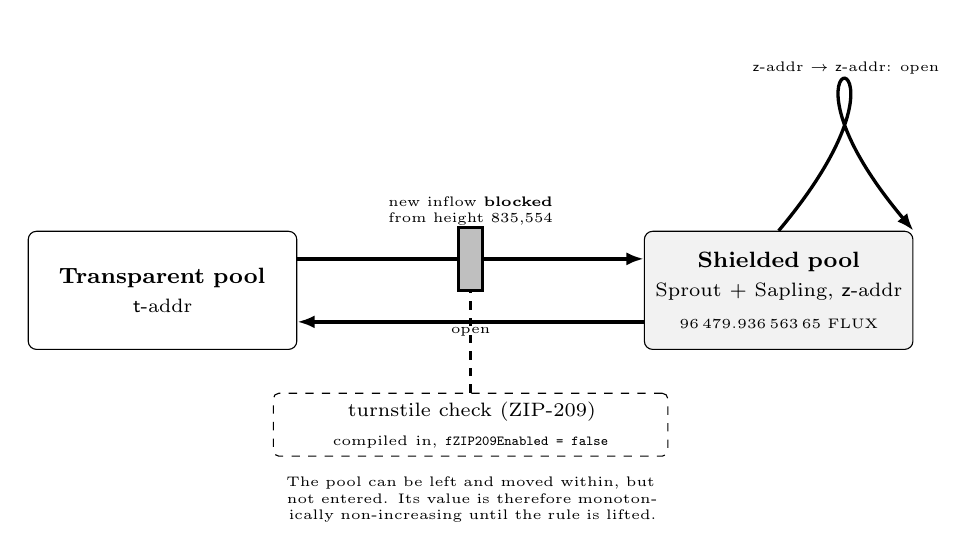
\begin{tikzpicture}[
  font=\footnotesize,
  pool/.style={draw, rounded corners=3pt, minimum height=15mm, text width=32mm, align=center,
               inner sep=3pt},
  arr/.style={-{Latex[length=2.2mm]}, very thick},
  lbl/.style={font=\tiny, align=center, inner sep=1.5pt},
]
  \node[pool] (t) {\textbf{Transparent pool}\\[1pt]{\scriptsize \taddr}};
  \node[pool, right=44mm of t, fill=black!5] (z)
     {\textbf{Shielded pool}\\[1pt]{\scriptsize Sprout + Sapling, \zaddr}\\[2pt]
      {\tiny \num{96479.93656365}\,\flux}};

  % t -> z : blocked
  %% yshift clears the 8mm blocking bar drawn at the same midpoint, which used to
  %% print straight through this label.
  \draw[arr] ([yshift=4mm]t.east) -- node[lbl, above, pos=0.5, yshift=3.5mm]
      {new inflow \textbf{blocked}\\from height 835{,}554} ([yshift=4mm]z.west);
  \node[draw, very thick, minimum width=3mm, minimum height=8mm, fill=black!25]
      at ($([yshift=4mm]t.east)!0.5!([yshift=4mm]z.west)$) {};

  % z -> t : open
  \draw[arr] ([yshift=-4mm]z.west) -- node[lbl, below, pos=0.5]
      {open} ([yshift=-4mm]t.east);

  % z -> z loop
  \draw[arr] (z.north) to[out=50, in=130, looseness=5]
      node[lbl, above] {\zaddr $\to$ \zaddr: open} (z.north east);

  % turnstile gate, present but inactive
  \node[draw, dashed, rounded corners=2pt, below=13mm of $(t)!0.5!(z)$, text width=48mm,
        align=center, inner sep=3pt] (ts)
      {\scriptsize turnstile check (ZIP-209)\\[1pt]{\tiny compiled in, \texttt{f\allowbreak{}ZIP209Enabled = false}}};
  \draw[dashed, thick] (ts) -- ($(t.east)!0.5!(z.west)$);

  \node[lbl, below=2mm of ts, text width=62mm]
      {The pool can be left and moved within, but not entered. Its value is therefore
       monotonically non-increasing until the rule is lifted.};
\end{tikzpicture}
\caption{Value flow between \fluxd's transparent and shielded pools, showing the turnstile check as
present in code but inactive, and the height-835{,}554 restriction on new transparent-to-shielded
inflow. \shipped, \srccode{fluxd/\allowbreak{}src/\allowbreak{}main.cpp}{1398-1408,3838-3862}; \srccode{fluxd/\allowbreak{}src/\allowbreak{}chainparams.h}{200}.}
\label{fig:shielded-value-flow}
\end{figure}

\subsection{Supply accounting}
\label{sec:supply-accounting}

\fluxd exposes shielded-pool accounting through a \texttt{valuePools} array on the
\texttt{getblockchaininfo} and \texttt{getblockheader} RPCs, with one entry per pool (\texttt{id}
\texttt{"sprout"} or \texttt{"sapling"}), each carrying \texttt{monitored}, \texttt{chainValue},
\texttt{chainValueZat}, \texttt{valueDelta}, and \texttt{valueDeltaZat} (\shipped,
\srccode{fluxd/\allowbreak{}src/\allowbreak{}rpc/\allowbreak{}blockchain.cpp}{84-101}), reported both per block
(\srccode{fluxd/\allowbreak{}src/\allowbreak{}rpc/\allowbreak{}blockchain.cpp}{279-282}) and at the chain tip
(\srccode{fluxd/\allowbreak{}src/\allowbreak{}rpc/\allowbreak{}blockchain.cpp}{1068-1071}). These fields are what a supply audit would read
from: the total issued supply $\supply$ that \S5 defines is, by the roadmap's own description, ``the
transparent set plus the shielded pools'' \srcroadmap{flux-roadmap-public.md:185}, and the roadmap
states that this reconciles with the emission model to within 0.0005\%
\srcroadmap{flux-roadmap-public.md:185}.

The accounting fields are computed and exposed regardless of the turnstile switch discussed in
\S\ref{sec:switched-off}. What the disabled switch removes is not the numbers themselves but the
consensus-enforced invariant that would make a negative pool balance — the signature of exactly the
kind of undetected forgery discussed in \S\ref{sec:trusted-setup} — impossible to sustain on-chain
without triggering block rejection. \texttt{valuePools} is a reporting surface; turnstile enforcement
is the check that would make the report trustworthy on its own. With \texttt{f\allowbreak{}ZIP209Enabled = false}
on both live networks, \fluxd today performs no automated on-chain detection of a negative Sprout or
Sapling pool balance outside of whatever manual monitoring an operator does against the
\texttt{valuePools} field (\shipped, \srccode{fluxd/\allowbreak{}src/\allowbreak{}chainparams.h}{200}). This is the same gap
named in \S\ref{sec:switched-off} and G9, restated here in its supply-accounting form because it is
what connects this section to \S5's supply function: $\supply$ as defined there is only as trustworthy
as the pool-balance fields that compose it, and those fields currently carry no consensus-level
non-negativity guarantee.

\subsection{The RPC surface}
\label{sec:rpc-surface}

The wallet RPC command table exposes the full set of z-address operations
(\shipped, \srccode{fluxd/\allowbreak{}src/\allowbreak{}wallet/\allowbreak{}rpcwallet.cpp}{4994-5021}). This is the toolkit \S21's
private-payment construction is built on, and it is enumerated here precisely rather than by example:

\begin{description}
\item[Key and address management] \texttt{z\_getnewaddress}, \texttt{z\_listaddresses},
  \texttt{z\_exportkey}, \texttt{z\_importkey}, \texttt{z\_exportviewingkey},
  \texttt{z\_importviewingkey} ($\viewkey$), \texttt{z\_exportwallet}, \texttt{z\_importwallet}
  (\shipped, \srccode{fluxd/\allowbreak{}src/\allowbreak{}wallet/\allowbreak{}rpcwallet.cpp}{4994-5018}). Full and incoming Sapling viewing
  keys ($ak,nk,ovk$ and the incoming-viewing-key form) are the objects these last two RPCs move
  (\shipped, \srccode{fluxd/\allowbreak{}src/\allowbreak{}flux/\allowbreak{}Address.hpp}{32-222}), and \texttt{zip32.h} carries the
  ZIP-32 seed fingerprint and parent-FVK tag fields that identify derived keys (\shipped,
  \srccode{fluxd/\allowbreak{}src/\allowbreak{}flux/\allowbreak{}zip32.h}{32,55,101}).
\item[Balance inspection] \texttt{z\_listreceivedbyaddress}, \texttt{z\_listunspent},
  \texttt{z\_getbalance}, \texttt{z\_gettotalbalance} (\shipped,
  \srccode{fluxd/\allowbreak{}src/\allowbreak{}wallet/\allowbreak{}rpcwallet.cpp}{4994-5018}).
\item[Value movement] \texttt{z\_sendmany}, \texttt{z\_shieldcoinbase},
  \texttt{z\_setmigration}\slash\texttt{z\_getmigrationstatus} (dead post-height-835{,}554, \S\ref{sec:switched-off}),
  and \texttt{z\_mergetoaddress} — the last gated behind an explicit \texttt{-\allowbreak{}zmergetoaddress} flag
  (\shipped, \srccode{fluxd/\allowbreak{}src/\allowbreak{}wallet/\allowbreak{}rpcwallet.cpp}{4463-4466}; \srccode{fluxd/\allowbreak{}src/\allowbreak{}init.cpp}{905-906}).
\item[Asynchronous operation tracking] \texttt{z\_getoperationstatus}, \texttt{z\_getoperationresult},
  \texttt{z\_listoperationids} (\shipped, \srccode{fluxd/\allowbreak{}src/\allowbreak{}wallet/\allowbreak{}rpcwallet.cpp}{4994-5018}).
\item[Raw Sprout operations] \texttt{zcbenchmark}, \texttt{zcrawkeygen}, \texttt{zcrawjoinsplit},
  \texttt{zcrawreceive}, \texttt{zcsamplejoinsplit} (\shipped,
  \srccode{fluxd/\allowbreak{}src/\allowbreak{}wallet/\allowbreak{}rpcwallet.cpp}{4994-5021}).
\item[Payment disclosure] \texttt{z\_getpaymentdisclosure} and \texttt{z\_validatepaymentdisclosure}
  are registered under the RPC category \texttt{"disclosure"} (\shipped,
  \srccode{fluxd/\allowbreak{}src/\allowbreak{}wallet/\allowbreak{}rpcwallet.cpp}{5020-5021}), backed by the note-decryption path described
  in \S\ref{sec:shielded-machinery}. They are compiled in but off by default: both require
  \texttt{f\allowbreak{}Experimental\allowbreak{}Mode}, whose global default is \texttt{false} (\inprogress,
  \srccode{fluxd/\allowbreak{}src/\allowbreak{}main.cpp}{77}), set only via \texttt{-\allowbreak{}experimentalfeatures}, plus their own
  per-feature flag; enabling one without the other aborts startup with an explicit error
  (\inprogress, \srccode{fluxd/\allowbreak{}src/\allowbreak{}init.cpp}{895,903-904}). Payment disclosure is present code, not
  an active default.
\end{description}

Payment disclosure and viewing-key export together give a selective-disclosure capability — reveal a
transaction, or a stream of incoming payments, to a chosen third party without revealing anything
else — that is exactly the primitive \S21's payer/network problem needs; \S21 states the construction
it builds from this surface, or states precisely where the surface stops short of it.

\subsection{Post-quantum scope: what is bounded, and why}
\label{sec:pq-scope}

Groth16 as deployed here is a pairing-based SNARK over BLS12-381 — the 192-byte proof format fixed by
\texttt{GROTH\_PROOF\_SIZE} is exactly the compressed $G_1\|G_2\|G_1$ encoding this construction
uses~\citep{groth2016size} (\shipped, \srccode{fluxd/\allowbreak{}src/\allowbreak{}flux/\allowbreak{}JoinSplit.hpp}{22-26}). Its soundness
rests on pairing- and discrete-log-type hardness assumptions over that curve, which a
sufficiently large quantum computer running Shor's algorithm breaks. This is a property of the
scheme itself, not of Flux's use of it, and it holds regardless of who ran the trusted setup in
\S\ref{sec:trusted-setup}: \textbf{the Sapling shielded layer, as deployed, is not post-quantum
secure.} No post-quantum-related code, comment, or TODO exists anywhere under \texttt{src/} —
a repository-wide search for \texttt{quantum} returns zero hits (\shipped, \srccode{fluxd/\allowbreak{}src}{grep -rn quantum, zero matches}).

Given that, the team's stated position is to bound the post-quantum migration deliberately rather
than claim more than the deployed cryptography supports. What is to become post-quantum is
consensus, transparent transactions, and the keys securing them; the shielded layer is explicitly
placed out of scope for now, with post-quantum privacy construction to follow later as the field
matures \srcintent{design intake} (\vision; after the retirement decision of
\S\ref{sec:shielded-retirement}, any such construction is a future option, not a scheduled item).
This scope decision is presented in the design intake
as coherent and defensible rather than as an admitted gap, on the reasoning that privacy is already
optional at the protocol level (the roadmap's own position, quoted at the head of this section), so a
transparent-layer-first migration does not leave the
part of the system that everyone must use exposed while the part that is opt-in waits. The paper
adopts that framing because the alternative is worse: an unqualified ``quantum-ready'' claim made
while a live Groth16-based shielded pool sits underneath it would be a claim a reviewer familiar with
the scheme would immediately falsify. A scope statement this specific — consensus and transparent
keys first, shielded privacy deferred and named as deferred — is the position that survives that
scrutiny; a blanket claim is not.

One distinction has to be kept strict, because it is the likeliest error in this area. Removing a
trusted setup and achieving post-quantum security are two different properties, and a future
construction can have either without the other. Halo2, the proof system behind Zcash's Orchard
pool, eliminates the per-circuit trusted setup entirely by replacing it with a transparent, universal
setup~\citep{bowe2019halo} — but it does so by resting on discrete-log hardness over a different
curve, which is exactly as vulnerable to a quantum adversary as the pairing assumption Groth16 uses.
Adopting Halo2/Orchard, discussed next, would answer the trusted-setup question and would do nothing
for the post-quantum question. The two must not be conflated in either direction.

\subsection{What a migration to Orchard/Halo2 would, and would not, buy}
\label{sec:orchard-migration}

Orchard is absent from \fluxd today (\S\ref{sec:shielded-machinery}), and no committed timeline or
specific target construction exists yet: the roadmap places ``Chain privacy implementation'' in H2
2027, explicitly ``on the schedule set by the Q4 2026 plan''
\srcroadmap{flux-roadmap-public.md:158} (\planned), and states that the Q4 2026 privacy groundwork
work is where ``which shielded construction to adopt'' is still to be settled
\srcroadmap{flux-roadmap-public.md:177} (\planned). Whether that construction turns out to be
Orchard/Halo2 specifically, some other Zcash-lineage successor, or something else is not yet decided
by the team's own account, so this subsection is stated as \vision rather than as a scheduled item.

The argument for making that move is specific, not generic, and worth stating precisely: adopting a
Halo2-class proving system removes the inherited trusted setup described in
\S\ref{sec:trusted-setup} entirely, and that directly serves the stated decentralization requirement
— a chain whose privacy layer's soundness depends on a multi-party ceremony run once, by a fixed set
of participants, in 2018, is not decentralized in the same sense the rest of the design intake asks
for \srcintent{design intake} (\vision). That argument stands on its own regardless of the
post-quantum question, and the paper states it as such rather than bundling it with a PQ claim it
does not support (\S\ref{sec:pq-scope}).

What it would not buy is equally specific: no candidate successor construction under discussion is
post-quantum secure, so a migration to Orchard/Halo2 closes the trusted-setup gap while leaving the
shielded layer's long-term cryptographic exposure to a quantum adversary exactly where it is today.
The team's stated position on timing is to not pin one: ``We will not pin a date on a cryptographic
change before its audit is scoped. The direction is not in question''
\srcroadmap{flux-roadmap-public.md:177} (\planned). The paper records that position rather than
supplying a date the source does not give.

\subsection{Retiring the pools: the decision, and the measurements behind it}
\label{sec:shielded-retirement}

\textbf{Both shielded pools are to be retired} \srcintent{design intake}
(\planned). The team raised the possibility alongside reopening and migrating --- destroying the
existing pool outright to simplify the chain, reduce maintained code and obtain a more thorough audit
of what remains, with a stated preference for C++ over Rust
\srcintent{design intake} --- and, presented with the analysis below, took it.

This subsection records the measurement that motivated the decision, the constraint that made it
sharper than it first appears, and the schedule. The argument is retained in full rather than
compressed to its outcome, because a decision to destroy a live mechanism holding user value should
remain auditable against the reasoning that produced it.

\paragraph{What is actually in the pools.} Both legacy pools are live and both are small.

\begin{table}[H]
\centering\footnotesize
\caption{Shielded pool balances at height \num{2917115}, from \fluxd's own \texttt{valuePools}
reporting surface. Circulating supply is the emission model's value at that height
(\Cref{sec:monetary-policy}). \shipped
\srcmeasured{api.runonflux.io/daemon/getblockchaininfo, field \texttt{valuePools}}{2026-09-03}.}
\label{tab:pool-balances}
\begin{tabular}{@{}lrr@{}}
\toprule
Pool & Balance (\flux) & Share of circulating supply \\
\midrule
Sprout (JoinSplit lineage) & \num{19291.17735041} & \SI{0.0045}{\percent} \\
Sapling & \num{77188.75921324} & \SI{0.0180}{\percent} \\
\midrule
Total shielded & \textbf{\num{96479.93656365}} & \textbf{\SI{0.0225}{\percent}} \\
\bottomrule
\end{tabular}
\end{table}

\noindent Three facts follow, and together they carry the argument. First, the combined shielded
balance is about one part in \num{4500} of circulating supply. Second, the balance is
\emph{monotonically non-increasing}: the transparent-input gate of
\S\ref{sec:switched-off} rejects any transaction carrying both a transparent input and a
shielded output, so value has been unable to enter either pool since height \num{835554}
\srccode{fluxd/src/main.cpp}{1398--1408}. Third --- and this is the fact most often missed --- the
gate keys on \texttt{tx.vin.size()} alone, so \zaddr${}\to{}$\zaddr and
\zaddr${}\to{}$\taddr transactions remain fully valid. The pools are sealed from outside and
unimpaired within: existing holders retain full use and can exit at will.

\paragraph{The constraint that decides it.} The stated preferences --- newest Zcash work, less code,
a more thorough audit, and C++ over Rust --- cannot all be satisfied, because they point in opposite
directions. Sapling proving and verification in \fluxd run through \texttt{librustzcash}
(\S\ref{sec:shielded-machinery}), which is Rust. Orchard's Halo2 proving system exists as a Rust
implementation and has no production C++ equivalent. Zcash's own trajectory has been to move
consensus-critical cryptography \emph{into} Rust, not out of it. So ``port the newest Zcash work''
and ``prefer C++'' are not jointly achievable: adopting newer Zcash cryptography means more Rust in
the consensus path, not less \srcinferred.

That leaves exactly three self-consistent positions, and the preference set selects among them
cleanly:

\begin{table}[H]
\centering\footnotesize
\caption{The three coherent options, against the team's own stated preferences.}
\label{tab:shielded-options}
\begin{tabular}{@{}lllll@{}}
\toprule
Option & Chain privacy & Rust in consensus & Trusted setup & Audit surface \\
\midrule
(A) Reopen Sapling & yes & retained & inherited, two ceremonies & unchanged, large \\
(B) Retire both pools & \textbf{none} & \textbf{removable} & \textbf{none} & \textbf{smallest} \\
(C) Retire, later adopt Orchard & deferred & increased & none (Halo2) & large, later \\
\bottomrule
\end{tabular}
\end{table}

\paragraph{Option (B) is the decision; (C) remains available later.} Four arguments, in order of
weight.

\begin{enumerate}
  \item \textbf{A shielded pool does not buy what the thesis needs.} The workload is public by
  construction. A Flux application specification is a permanent on-chain message, and the
  control plane serves the global specification set over a public endpoint
  \srccode{flux-domain-manager/src/services/flux/dataFetcher.js}{47-71}. What a tenant deploys, the
  resources it claims and the owner it binds to are therefore public whatever the payment rail does.
  Shielding the payment hides the \emph{funding source}, not the workload graph. That is a real but
  narrow benefit, and \S\ref{sec:private-payment} shows it is also the harder half to construct
  correctly.
  \item \textbf{Every stated preference points the same way.} (A) and (C) both keep or expand Rust in
  the consensus path; only (B) permits removing \texttt{librustzcash}, the JoinSplit and Sapling
  circuits, the note-commitment trees and the nullifier sets from the daemon. If a smaller,
  C++-centred, thoroughly audited consensus layer is the goal, (B) is the only option that delivers
  it.
  \item \textbf{It closes a supply-accounting gap the paper already documents.}
  \Cref{sec:supply-accounting} records that \texttt{valuePools} is a reporting surface with no
  consensus enforcement behind it: a negative pool balance --- the signature of an inflation bug in
  the shielded code --- would not by itself cause block rejection, because ZIP-209 turnstile
  enforcement is compiled in but dormant against unmodified upstream-Zcash checkpoint constants
  \srccode{fluxd/src/chainparams.cpp}{322-327}. Removing the pools removes that entire class of
  unauditable supply risk, and makes total supply exactly reconstructible from transparent UTXOs.
  For a design whose monetary section rests on supply transparency, that is a direct gain.
  \item \textbf{The value at risk is bounded and measured.} \num{96479.94}\flux, in a pool that
  cannot grow. This is the number the decision should be made against, and it is small enough that
  a generous migration window costs little and dishonours no one.
\end{enumerate}

\paragraph{The retirement schedule.} The decision is settled; the heights below were the paper's
recommendation and are confirmed by the author (Remark~\ref{rem:shield-schedule-confirmed}).

\begin{itemize}
  \item \textbf{Announcement at publication}, i.e. with this paper (2026-09-07), alongside the notice
  of the parallel-asset one-way switch at $\hopen$ (\S\ref{sec:pa-sequencing}). One consolidation
  message covering both is better than two, and the holder sets barely overlap.
  \item \textbf{Sunset at $\hshield = \num{3600000}$}, about 2027-04-27 at the \SI{30}{\second}
  target: \num{232} days after publication, \num{150000} blocks after $\hopen$ and \num{187502}
  blocks \emph{before} $\hpa$ \srcintent{08-answers-round-2.md, round 37}. After this height,
  transactions carrying \texttt{vShieldedSpend} or \texttt{vJoinSplit} are invalid; notes not swept
  are permanently unspendable. Seven and a half months is deliberately longer than the roughly
  five-month parallel-asset window (\S\ref{sec:bridging-migration}): that window ends in forfeiture
  to a named recipient, whereas this one ends in destruction, which warrants more notice for less
  value. The height is a consensus rule and must ship in a \texttt{fluxd} release ahead of it.
  \proposednote{Carry it in the \texttt{fluxd} upgrade the roadmap already plans for H1 2027
  (collateral maturity, \S\ref{sec:migration}), so that retirement adds no release of its own before
  \PNR{}.}
  \item \textbf{No change to exit paths during the window.} \zaddr${}\to{}$\taddr already works and
  needs no consensus change to keep working; the window requires an announcement, not a code change.
  \item \textbf{Activate ZIP-209 turnstile enforcement with Flux-correct constants for the duration
  of the window.} Whatever is decided about the pools' future, the current state --- enforcement
  code compiled in but dormant, parameterised by another chain's checkpoints --- is the worst of the
  available positions, because it carries the maintenance cost of the mechanism without its
  guarantee. During a drain-only window the turnstile is a cheap and exactly-correct safety net: the
  pool balance must only decrease, which is precisely what the turnstile checks.
  \item \textbf{Direct outreach, not announcement alone.} The holder set is small enough to make
  this tractable and small enough that a purely passive notice would be a poor effort.
\end{itemize}

\begin{remark}[Schedule confirmed]
\label{rem:shield-schedule-confirmed}
The heights above were proposed by this paper and are \textbf{confirmed by the author}
\srcintent{design intake}; the sunset was then brought forward to $\hshield = \num{3600000}$ and the
announcement to publication \srcintent{08-answers-round-2.md, round 37}. Activating ZIP-209 turnstile enforcement with Flux-correct constants for
the window remains this paper's recommendation, not a confirmed decision: round 11 confirmed the
numbers, and a switch is not a number \srcintent{design intake}. The retirement
decision and its heights are settled, and \S\ref{sec:private-payment}'s construction questions are
consequently not live (\Cref{rem:pp-conditional}).
\end{remark}

\begin{remark}[What retirement costs, stated without softening]
\label{rem:retirement-cost}
Three things are given up, and the paper names them rather than letting the argument above stand
unopposed.

\textbf{Flux will have no chain-level privacy.} Not reduced privacy --- none. Every transfer, every
balance and every payment for a deployment will be publicly linkable for anyone willing to do the
analysis, exactly as on Bitcoin. The design intake asked for privacy-preserving settlement rails
\srcintent{design intake}; after retirement the honest description is that Flux settles
transparently and treats payment privacy as an unsolved problem rather than a delivered feature.
\Cref{sec:pq-scope} and \S\ref{sec:private-payment} are the two places this paper previously
claimed otherwise, and both are now corrected.

\textbf{Value will be destroyed at $\hshield$.} Notes not swept before the sunset become
permanently unspendable. The bound is \num{96479.94}\flux{} and shrinking, and the window is long,
but this is confiscation by inaction and calling it anything softer would be dishonest. It is the
reason the schedule recommends direct outreach rather than announcement alone.

\textbf{The option is one-directional in practice.} Rebuilding a shielded pool later means adopting
Orchard/Halo2 or an equivalent --- a multi-year cryptographic project, in Rust, against the stated
language preference. Option~(C) remains formally available and should not be described as though it
were cheap.
\end{remark}

%% Drain this section's float queue before the next begins.
\FloatBarrier

\section{Private payment with public obligation}
\label{sec:private-payment}\label{sec:private-renewal}

Every node on the network must be able to decide, on its own and without asking anyone, whether the
workload it is about to run has been paid for. That decision has to be reproducible by thousands of
mutually distrusting machines from public data alone, which is precisely why the payment that answers
it is, today, a transparent transaction whose inputs name its sender. The tension this section
addresses is one sentence long: \emph{the network must be convinced that a deployment is funded while
learning neither who paid nor which payer belongs to which workload.} The workload itself is public
and must stay public --- a node cannot run a container whose image it is not told --- so the object to
hide is not the obligation but the payer, and the edge between the payer and the obligation. What
follows states that requirement formally, shows which parts of it the deployed Sapling toolkit already
satisfies, shows which part is unsatisfiable by construction and says so rather than omitting it,
measures the anonymity set that actually exists rather than assuming one, and names the single
consensus rule that gates the whole thing. The most important result in this section is a
\emph{negative scope} result: the general problem is smaller than it looks, and the part that remains
genuinely open is confined to one optional path.

\begin{remark}[Status of this section after the retirement decision]
\label{rem:pp-status}
\textbf{Flux is retiring both shielded pools} (\Cref{sec:shielded-retirement},
\srcintent{08-answers-round-2.md, round 10}). Every \emph{construction} in this section is therefore
inapplicable to the target architecture: there will be no pool to pay into, no Sapling output to
build a payment from, no anonymity set to grow, and no proving system to select. The section is
retained, unmodified in its technical content, for three reasons, and a reader should hold all three
in mind while reading it.

\begin{enumerate}
  \item \textbf{The requirement survives the decision.} \Cref{def:pp-pi} and \Cref{def:pp-ru} state what private
  payment for a public obligation must satisfy. That statement is independent of any construction and
  independent of whether Flux carries a shielded pool. If Flux ever revisits privacy --- via
  Orchard/Halo2 or otherwise --- this is the specification the work must meet, and it is written
  down here rather than needing to be rediscovered.
  \item \textbf{Two of its results are why retirement is defensible.}
  \S\ref{sec:pp-amount} proves amount hiding is unsatisfiable under \PNR{}, and
  \S\ref{sec:pp-scope} shows the residual problem is confined to one optional path. Together they
  establish that a shielded pool was buying considerably less than it appears to --- which is a load-
  bearing input to the decision, not a consolation after it.
  \item \textbf{The measurement is a permanent record.} \S\ref{sec:pp-anonymity} measures the
  anonymity set that actually existed on Flux. After retirement that measurement cannot be repeated,
  and it is the honest empirical answer to how much privacy the deployed pool ever provided.
\end{enumerate}

Read the constructions below as \emph{what would have been required}, not as what is planned. Where
the text says \planned{} of a shielded construction, that tag is now superseded by the retirement
decision and should be read as conditional on a pool existing.
\end{remark}

\begin{remark}[Symbols introduced here]
This section uses, in addition to \texttt{notation.tex}: $m_\app$ for the registration or update
message of application $\app$; $H_\app \defeq \mathsf{SHA256}(m_\app)$ for its hash, the value FluxOS
places in \texttt{OP\_RETURN}; $e_\app$ for the paid-through height; $A_{\mathrm{sink}}$ for the
payment sink, \S7's $\mathsf{sink}$; $v$ for a paid amount in \sat; $v_{\mathrm{bal}}$ for a Sapling \texttt{valueBalance};
$u$ for an individual FluxOS node; $\mathsf{AS}$ for an anonymity set; $\epsilon_{\mathrm{sc}}$ for a
side-channel advantage; $\tree_{\mathrm{ent}}$ and $\mathsf{rt}$ for an entitlement tree and its root;
$s$ for a credential secret; $j$ for an epoch index and $T_{\mathrm{ep}}$ for an epoch length; and
$\mathsf{xsk}$ for a ZIP-32 child spending key. These are proposed additions to the notation index
(Appendix~D) and are used nowhere else in the paper.
\end{remark}

\subsection{The verifier, and the requirement pair}
\label{sec:pp-requirements}

\subsubsection{What is public by construction}

Three things are public because the system cannot function otherwise, and it is worth separating them
before any privacy claim is made.

\begin{enumerate}
  \item \textbf{The workload.} An application's public part
    $\mathsf{spec}_{\mathrm{pub}}(\app) = (\mathsf{name}, H_\app, \mathsf{owner}, \ninst, \dur,
    \hgt_0, \mathsf{enterprise?})$ is stored by every node, because placement is opportunistic
    self-selection and any node may be the one that runs $\app$ (\shipped, \srccode{flux/\allowbreak{}ZelBack/\allowbreak{}src/\allowbreak{}services/\allowbreak{}appDatabase/\allowbreak{}registryManager.js}{1714}).
    Content is a separate matter: of the \num{1195} deployed applications, \num{972} publish their
    \texttt{compose} block in the clear and \num{223} (\qty{18.7}{\percent}) are enterprise records
    whose \texttt{compose} and \texttt{contacts} are stored zeroed
    \srcmeasured{api.runonflux.io/\allowbreak{}apps/\allowbreak{}globalappsspecifications}{2026-09-03}.
  \item \textbf{The paid-through height.} $e_\app$ must be a public function of the chain, or nodes
    disagree about whether to keep running a container.
  \item \textbf{The amount, under \PNR.} This is derived rather than chosen, and
    \S\ref{sec:pp-amount} proves it.
\end{enumerate}

What is \emph{not} required to be public is the identity of the party that moved the value, and the
association between that party and the application. That is the whole of the privacy goal here, and
stating it this narrowly is what makes the rest of the section tractable.

\subsubsection{The verifier}

\begin{definition}[Funding scheme and verifier]
\label{def:pp-scheme}
Let $\mathsf{Apps}$ be the set of application identifiers, $\mathcal{C}$ the set of chain prefixes,
$\mathsf{Tx}$ the set of transactions and $\mathsf{Msg}$ the set of FluxOS messages. A \emph{funding
scheme} is a pair $(\mathsf{Fund}, \mathsf{Verify})$ with
\[
  \mathsf{Fund} : \principal \times \mathsf{Apps} \longrightarrow \mathsf{Tx} \times (\mathsf{Msg} \cup \{\varepsilon\}),
  \qquad
  \mathsf{Verify}_u : \mathsf{Apps} \times \mathbb{N} \times \mathcal{C} \longrightarrow \mathbb{N} \cup \{\bot\},
\]
where $\mathsf{Fund}$ is run by a principal and $\mathsf{Verify}_u$ is run by FluxOS node $u$ on its
local chain prefix $C_{\le\hgt}$ and its local message store, returning a paid-through height $e_\app$
or $\bot$. Funded status is $\mathsf{Funded}(\app,\hgt) \defeq \indic{\hgt \le e_\app}$.
\end{definition}

\begin{assumption}[Verifier model, from \S2]
\label{ass:pp-verifier}
Node $u$ holds $C_{\le\hgt}$, the FluxOS temporary and permanent message sets, and \emph{no secret}:
no shared key, no issuer key, and no viewing key it did not derive from public data. Node $u$ needs no
message from any other verifier to evaluate $\mathsf{Verify}_u$. This is a description of the deployed
system, not a design preference: \texttt{explorerService.\allowbreak{}processInsight} recognises a payment by output
address and \texttt{OP\_RETURN} and \texttt{messageVerifier.\allowbreak{}checkAndRequestApp} promotes the
registration message, on every node, from chain data alone (\shipped,
\srccode{flux/\allowbreak{}ZelBack/\allowbreak{}src/\allowbreak{}services/\allowbreak{}explorerService.js}{309--345},
\srccode{flux/\allowbreak{}ZelBack/\allowbreak{}src/\allowbreak{}services/\allowbreak{}appMessaging/\allowbreak{}messageVerifier.js}{619--897}); CumulusVPN states the same property
of its gateways --- ``every gateway runs the same deterministic scan and therefore reaches the same
\texttt{paid\_until} map [\ldots] with no server-to-server coordination'' (\shipped, \srccode{cumulusvpn/\allowbreak{}gateway/\allowbreak{}internal/\allowbreak{}entitle/\allowbreak{}entitle.go}{1--5}).
\end{assumption}

\begin{assumption}[Adversary, from \S2]
\label{ass:pp-adversary}
The adversary $\adv$ is a node operator. It sees the whole chain, the public specification of every
application, all FluxOS gossip, and the client traffic arriving at the nodes it runs; it may run any
number of nodes (the measured maximum under one signing key is \num{237}, \qty{3.7}{\percent} of the
fleet \srcmeasured{api.runonflux.io/\allowbreak{}daemon/\allowbreak{}listzelnodes}{2026-09-03}); it may be the \emph{owner} of
the application whose payer it wants to identify; and it may hold shielded funds. It is bounded by
$\advbudget$ for anything requiring capital and is otherwise probabilistic polynomial time.
\end{assumption}

\subsubsection{The hard requirements}

\begin{definition}[Public obligation]
\label{def:pp-obligation}
A funding scheme satisfies \emph{public obligation} if:
\begin{description}
  \item[V0 (no secret).] $\mathsf{Verify}_u$ is a deterministic function of $C_{\le\hgt}$ and public
    messages, for every $u$.
  \item[S (soundness).] For every PPT payer $\adv$,
    \[
      \Pr\!\left[\mathsf{Verify}_u(\app,\hgt,C_{\le\hgt}) = e > \hgt
      \ \wedge\ \textstyle\sum \text{value confirmed to } A_{\mathrm{sink}} \text{ bound to } H_\app \text{ by } \hgt < \price(\app)\right]
      \le \mathrm{negl}.
    \]
  \item[C (consistency).] Honest $u, u'$ with the same chain prefix return the same $e_\app$.
  \item[L (liveness under partition).] $\mathsf{Verify}_u$ requires no message from any other party; a
    partitioned node evaluates on its local prefix and converges when the prefix does.
  \item[D (no double-funding).] One confirmed transfer contributes to at most one pair
    $(\app,\text{period})$.
\end{description}
\end{definition}

\begin{definition}[Payer indistinguishability, PI]
\label{def:pp-pi}
$\adv$ names two principals $\principal_0,\principal_1$, each able to fund, and an application $\app$;
$\adv$ may own $\app$ and any set of nodes. The challenger draws $b \in \{0,1\}$ uniformly and runs
$\mathsf{Fund}(\principal_b,\app)$; $\adv$ observes the resulting chain and network state and outputs
$b'$. Define
\[
  \mathrm{Adv}^{\mathrm{PI}}(\adv) \defeq \left|\Pr[b'=b] - \tfrac12\right| \in [0,\tfrac12].
\]
The scheme has \emph{cryptographic} PI if $\mathrm{Adv}^{\mathrm{PI}}(\adv) \le \mathrm{negl}$ whenever
$\principal_0$ and $\principal_1$ fund from the same pool, at the same time, with the same amount. Its
\emph{effective} advantage is $\mathrm{negl} + \epsilon_{\mathrm{sc}}$, where $\epsilon_{\mathrm{sc}}$
collects timing, amount and network-metadata leakage. \S\ref{sec:pp-anonymity} measures
$\epsilon_{\mathrm{sc}}$'s inputs rather than assuming them away.
\end{definition}

\begin{definition}[Renewal unlinkability, RU]
\label{def:pp-ru}
\emph{Payer-side:} for two funding events of the same $\app$ at periods $i \ne j$, $\adv$ cannot
distinguish whether one principal produced both. \emph{Cross-application:} for $\app \ne \app'$,
$\adv$ cannot distinguish whether one principal funded both. Two renewals of the same $\app$ are
linked by $H_\app$ by construction --- that is the obligation being public --- so RU never denotes
hiding \emph{that} $\app$ was renewed.
\end{definition}

\begin{definition}[Amount hiding, AH]
\label{def:pp-ah}
$\adv$ learns nothing about $v$ beyond $v \ge \price(\app)$.
\end{definition}

\begin{definition}[Forward secrecy, FS]
\label{def:pp-fs}
Compromise at period $i$ of all key material used to produce funding events of periods $\ge i$ does
not increase $\mathrm{Adv}^{\mathrm{PI}}$ and does not break RU for periods $< i$.
\end{definition}

Definitions~\ref{def:pp-obligation} and~\ref{def:pp-pi} are the \emph{hard} requirements;
Definitions~\ref{def:pp-ru}--\ref{def:pp-fs} are desirable, and \S\ref{sec:pp-shapes} states which are
achievable in which shape. Content privacy --- the hiding of $\mathsf{spec}_{\mathrm{priv}}(\app)$
from non-selected nodes by enterprise encryption --- is owned by \S10 and constrained here only in
that a funding scheme must not reduce it beyond what $\price(\app)$ already reveals. AH is the sole
point at which the two interact, which brings us to the first result.

\subsection{Amount hiding is unsatisfiable under PNR}\label{sec:pp-amounthiding}
\label{sec:pp-amount}

This is stated early because it is a genuine conflict between two of this paper's own mechanisms, and
because a reader who expects Zcash-style amount privacy on hosting payments should be disabused before
reading a construction that does not deliver it.

\begin{property}[Amount recovery from the fee pool]
\label{prop:pp-amount}
Let $\nodeshare(\hgt) \in (0,1]$ be the operator share at height $\hgt$ and write
$r(\hgt) = 100\,\nodeshare(\hgt) \in \{1,\dots,100\}$. Under \PNR{} (\S7, PT1--PT5), a hosting payment
of price $\price \in \mathbb{N}$ \sat{} credits
$A_\Phi = \left\lfloor r(\hgt)\,\price / 100 \right\rfloor$ \sat{} to the consensus fee pool $\pool$,
and the per-block drip $D_\hgt = \floorfrac{\pool_{\hgt-1}}{\drip}$ appears in the coinbase. Then
$A_\Phi$ is a public function of the chain, and consequently
\[
  \price \in \left[\ \frac{100\,A_\Phi}{r(\hgt)},\ \frac{100\,(A_\Phi+1)}{r(\hgt)} \right),
  \qquad \text{an interval of width } \frac{100}{r(\hgt)} \sat.
\]
At $\nodeshare = 0.20$ the price is recoverable to within \num{5}\sat; at the $\nodesharecap = 0.50$
ceiling, to within \num{2}\sat. Therefore \textbf{no funding scheme that settles through \PNR{}
satisfies AH} (Definition~\ref{def:pp-ah}).
\end{property}

\begin{proof}
Every node must compute $\pool_\hgt$ exactly in order to validate the coinbase, since $D_\hgt$ is a
consensus-checked function of $\pool_{\hgt-1}$ and a node that cannot compute the pool cannot decide
block validity. Hence $\pool_\hgt$ is a deterministic public function of $C_{\le\hgt}$, and so is each receipt's
$A_\Phi$: under PS4 of \S7 it is computed from the value of a transparent output paying
$A_{\mathrm{sink}}$, and the block's inflow $F_\hgt$ is the sum of these. Inverting the floor gives the stated
interval, whose width is $100/r$. Any scheme achieving AH would have to hide $A_\Phi$ from at least
one honest verifier, contradicting checkability of the coinbase; a hidden pool cannot drip a checkable
coinbase.
\end{proof}

\begin{remark}[\S7 and \S21 cannot both have what they want]
\label{rem:pp-conflict}
The resolution recorded in this paper is that amount privacy is \textbf{out of scope for
\PNR-typed payments, by construction rather than by omission}. The cost is asymmetric: for the
\num{972} public-content applications it is nil, because $\price$ is already a public function of a
public specification; for the \num{223} enterprise applications the price reveals
$\langle \pricevec, \resvec \rangle$, a coarse size fingerprint of encrypted content. The only escape
--- exempting a payment class from \PNR{} --- contradicts \S7's requirement that all hosting revenue
settle through the split, and is left as an open decision (Q5, Table~\ref{tab:pp-open}).
\end{remark}

\subsection{Three shapes, kept apart}
\label{sec:pp-shapes}

Most of the difficulty attributed to ``private payment on Flux'' comes from conflating three problems
whose hardness differs sharply. Table~\ref{tab:pp-shapes} separates them, and every later claim in
this section is scoped to one of the three.

\begin{table}[H]
\centering
\small
\caption{The three shapes of the private-payment problem. Only shapes B and C carry a standing object
that must be re-proved; shape A does not, which is the content of
Proposition~\ref{prop:pp-scope}.}
\label{tab:pp-shapes}
\begin{tabular}{@{}p{0.06\linewidth}p{0.20\linewidth}p{0.24\linewidth}p{0.20\linewidth}p{0.18\linewidth}@{}}
\toprule
& \textbf{The obligation names} & \textbf{Example} & \textbf{What must be hidden} & \textbf{Maturity} \\
\midrule
\textbf{A} & a public workload $H_\app$, which every node must know in order to run it &
application registration and renewal; the direct path of \S16 &
the payer &
\planned; deployed circuits, gated on \S\ref{sec:pp-blocker} \\
\addlinespace
\textbf{B} & a private user: a pseudonym whose only public attribute is ``paid until $e$'' &
CumulusVPN, memo $=\mathsf{base58}(\mathsf{SHA256}(pk_t)[0{:}20])$ &
the link pseudonym\,$\leftrightarrow$\,payment, \emph{and} pseudonym\,$\leftrightarrow$\,payer &
\vision; needs a circuit Flux does not have \\
\addlinespace
\textbf{C} & a standing balance debited over time &
deposited credits with auto-renewal, the credit path of \S16 &
the payer, and the link between successive debits &
\planned; reduces to A when the renewer is the payer's own agent \\
\bottomrule
\end{tabular}
\end{table}

Table~\ref{tab:pp-props} then states, per shape, which requirement is hard, which is desirable, and
which cannot be had. It is the map for the rest of the section.

\begin{table}[H]
\centering
\small
\caption{Requirements per shape. ``hard'' = a mechanism is not acceptable without it; ``desirable'' =
wanted, and its absence is stated rather than hidden.}
\label{tab:pp-props}
\begin{tabular}{@{}lllll@{}}
\toprule
\textbf{Property} & \textbf{A, direct} & \textbf{C, own agent} & \textbf{C, third-party renewer} & \textbf{B, CumulusVPN-class} \\
\midrule
V0, S, C, L & hard & hard & hard & hard \\
D & hard & hard & hard & vacuous (time-based) \\
PI vs.\ the network & hard & hard & hard & hard, vs.\ the gateway \\
PI vs.\ the renewer & n/a & n/a & desirable; \textbf{open} (R2) & n/a \\
PI, transparent payer & impossible & --- & --- & desirable; needs A \\
RU payer-side & from PI per event & hard & hard & hard, across epochs \\
RU cross-application & desirable & desirable & desirable & --- \\
AH & \textbf{unsatisfiable} (Prop.~\ref{prop:pp-amount}) & unsatisfiable & unsatisfiable & n/a, fixed price \\
FS & desirable & desirable & desirable & desirable \\
\bottomrule
\end{tabular}
\end{table}

\subsection{The scope result}
\label{sec:pp-scope}

The proposition below is the most consequential finding in this section, because it decides how much
of the paper's agent-native argument depends on an unsolved problem. It says: not much.

\begin{proposition}[No new relation is required for shape A]
\label{prop:pp-scope}
Let $\mathsf{Verify}_u$ be the deployed FluxOS funding rule of \S\ref{sec:pp-deployed}. Then:
\begin{enumerate}
  \item[(i)] $\mathsf{Verify}_u(\app,\hgt,C_{\le\hgt})$ depends on $C_{\le\hgt}$ only through the set
    of confirmed \emph{funding events}, where a funding event is a confirmed transaction carrying a
    transparent output $(A_{\mathrm{sink}}, v)$ together with $\mathsf{OP\_RETURN} = H_\app$. Between
    funding events, no predicate over hidden state is evaluated.
  \item[(ii)] There exists a funding scheme satisfying V0, S, C, L, D and cryptographic PI
    (Definitions~\ref{def:pp-obligation}, \ref{def:pp-pi}) whose only zero-knowledge component is the
    Sapling spend statement and the Sapling output statement, both already verified by every
    \fluxd{} node at consensus (\shipped,
    \srccode{fluxd/\allowbreak{}src/\allowbreak{}main.cpp}{1447--1482}, \srccode{fluxd/\allowbreak{}src/\allowbreak{}primitives/\allowbreak{}transaction.h}{155--242}).
  \item[(iii)] Consequently no relation outside the deployed circuits is required for shape A, and in
    particular ``a statement proving that a note was spent to a known application address without
    revealing the sender'' is not a new circuit: it is the Sapling spend statement with a transparent
    recipient.
\end{enumerate}
\end{proposition}

\begin{proof}[Proof sketch]
\emph{(i)} By inspection of the deployed rule (\S\ref{sec:pp-deployed}): $e_\app$ is assigned once per
funding event from $(v, \hgt', \dur(m_\app))$ and is never re-derived; $\mathsf{Verify}_u$ thereafter
compares two integers. There is therefore no standing obligation and nothing to prove repeatedly.
\emph{(ii)} Take Construction~\ref{con:pp-a} below. Its verifier is unchanged from the deployed one
because the FluxOS scanner keys on outputs and \texttt{OP\_RETURN} and never on inputs; V0, S, C, L, D
hold by the same argument as for the transparent path, since the value transfer is still a confirmed
transparent output to $A_{\mathrm{sink}}$. Cryptographic PI reduces to Sapling spend
indistinguishability: two funding transactions produced by $\principal_0$ and $\principal_1$ spending
notes of sufficient value differ only in $\nf$, $\mathsf{cv}$, $\mathsf{rk}$, $\zkproof$ and the
change-note ciphertext, each of which is hiding under Sapling's stated assumptions
\citep{zcashprotocol}; the number of spend and output descriptions, the anchor and the fee are not
hidden, so the builder must hold them equal across payers or they fall under $\epsilon_{\mathrm{sc}}$.
\emph{(iii)} Immediate from (i) and (ii): the verifier needs $v \ge \price$,
the binding of the transfer to $H_\app$, and that $v$ actually moved. The first two are transparent
fields; the third is exactly what the binding signature and the spend statement establish. No
statement \emph{about the application} is proved in zero knowledge, because the application is public.
\end{proof}

\begin{corollary}[Agent-native direct payment]
\label{cor:pp-agent}
When the renewing party is the tenant's own agent, shape C reduces to shape A composed with ZIP-32
child-key derivation (\shipped, \srccode{fluxd/\allowbreak{}src/\allowbreak{}flux/\allowbreak{}zip32.h}{53--136}): the ``balance'' is the
value of the notes held under a derived child key, it exists nowhere as protocol state, and each
renewal is an independent shape-A funding event. \textbf{Agent-native direct payment therefore
collapses to a plain Sapling spend plus ZIP-32.}
\end{corollary}

\begin{corollary}[Blast radius]
\label{cor:pp-blast}
The hard version of the problem --- repeated unlinkable proofs against a hidden standing object ---
arises only when something hidden must be \emph{reused} by a party that must not learn the link. That
is (a) shape C with a \emph{third-party} renewer, and (b) shape B for payers who cannot or will not
use the shielded pool. The agent-native argument of \S18 survives with the general problem still open,
and the exposure is limited to the optional credit path of \S16.
\end{corollary}

\begin{remark}[Constructible is not private]
\label{rem:pp-constructible}
Proposition~\ref{prop:pp-scope} is a statement about the \emph{relation to be proved}, not about
deployability or about realised privacy. Construction~\ref{con:pp-a} is constructible over deployed
circuits; whether it is private in practice depends on the size of the payer's anonymity set
(\S\ref{sec:pp-anonymity}) and on a consensus rule that currently forbids entering the pool at all
(\S\ref{sec:pp-blocker}). The paper claims only the first until the measurement M1 is taken. The
limitation is a result, not a consolation: knowing that three-quarters of the problem needs no new
cryptography is worth more than a construction for all of it that nobody has.
\end{remark}

\subsection{The blocker: the shielded pool cannot be entered}
\label{sec:pp-blocker}

\begin{assumption}[The pool is closed --- \shipped, and it gates everything below]
\label{ass:pp-closed}
Since \texttt{UPGRADE\_FLUX} at mainnet height \num{835554},
\texttt{Contextual\allowbreak{}Check\allowbreak{}Transaction} rejects any transaction that carries transparent inputs
($\mathtt{tx.vin.size()} > 0$) together with any new shielded output --- any non-empty
\texttt{vJoinSplit} or \texttt{v\allowbreak{}Shielded\allowbreak{}Output} --- with reject reason
\texttt{bad-\allowbreak{}txns-\allowbreak{}fluxrebrand-\allowbreak{}vprivacy-\allowbreak{}not-\allowbreak{}empty}
(\shipped, \srccode{fluxd/\allowbreak{}src/\allowbreak{}main.cpp}{1398--1408}). The in-source comment states the intent: ``we no
longer want to allow coins to go into the privacy pool''. The rule does not inspect
\texttt{tx.\allowbreak{}v\allowbreak{}Shielded\allowbreak{}Spend}, so $\zaddr \to \zaddr$ and $\zaddr \to \taddr$ transactions remain valid.
\textbf{Shielded value can move and can leave; it cannot enter.} This is a Flux-original consensus
policy, not an inherited Zcash ZIP --- a distinction \S20 must preserve.
\end{assumption}

\begin{corollary}[Who can use construction A today]
\label{cor:pp-who}
Construction~\ref{con:pp-a} would be available only to holders of value shielded before
Assumption~\ref{ass:pp-closed} took effect in April 2021: \num{77188.75921324}\flux{} in the Sapling
pool and \num{19291.17735041}\flux{} in the Sprout pool at chain tip \num{2917115}, totalling
\num{96479.93656365}\flux{}
\srcmeasured{api.runonflux.io/\allowbreak{}daemon/\allowbreak{}getblockchaininfo (valuePools)}{2026-09-03}. Against issued
supply of \num{429466823.97}\flux{} (\S5) that is \qty{0.0225}{\percent}. The pool has been closed for
\num{2081561} blocks, approximately \num{5.4} years of wall clock, and its value is
monotonically non-increasing: every $\zaddr \to \taddr$ hosting payment removes a participant's value
from it and can never be replaced.
\end{corollary}

Two consequences deserve to be stated plainly rather than buried. First, the roadmap's privacy items
--- ``we are bringing private transactions back'', ``shielded by default in the wallets we make'' ---
were \textbf{never wallet-integration tasks}: re-opening $\taddr \to \zaddr$ is a consensus change.
That distinction outlives the decision that followed it, because it is what made the roadmap's
sequencing wrong rather than merely optimistic. \textbf{Reopening is now cancelled}: both pools are
to be retired instead \srcintent{08-answers-round-2.md, round 10} (\planned,
\S\ref{sec:shielded-retirement}). Second, capacity was never the constraint and membership was: at
the list-price revenue of the entire measured population --- \num{3817.62}\flux{} per
\num{30.56}-day period under \Cref{def:price} as corrected, of which \num{1784.97}\flux{}
(\SI{46.8}{\percent}, over \num{247} applications) is deployed by the Foundation's own identities and
\num{2032.65}\flux{} (\SI{53.2}{\percent}, over \num{948}) is third-party
\srcdoc{scripts/21-private-renewal.py} --- the Sapling pool alone would have funded the whole
network's hosting for \num{1.69} years, or \num{3.18} years of third-party hosting alone.

The split is taken on the specification's \texttt{owner} field --- the ZelID --- and not on the
address that paid, and the distinction is load-bearing rather than pedantic. Under the custodial path
of \S\ref{sec:paying-for-capacity} the service holds both the user's ZelID key and their payment key
and signs on their behalf (C42), so a card-paid customer deployment settles \emph{from a
Foundation-held address while belonging to the customer's ZelID}. Attributing by payer would count
every such deployment as the Foundation's own and understate third-party demand by however much of it
arrives that way. \settlednote{attribution is by \texttt{owner} ZelID. Of the four
Foundation-configured identities, three own nothing or nearly nothing --- \texttt{usersToExtend}
(current) and \texttt{fluxTeamFluxID} own no applications and \texttt{fluxSupportTeamFluxID} owns one
--- which is what the configuration implies, since \texttt{usersToExtend} confers permission to
extend an application \emph{on behalf of its owner} rather than ownership
\srccode{flux/\allowbreak{}ZelBack/\allowbreak{}config/\allowbreak{}default.js}{229}. The entire
Foundation share therefore rests on one address, \texttt{196GJWyLxzAw\ldots}, holding 246 of the
\num{1195} applications. Its composition supports the attribution --- \texttt{FluxWhitepaper},
\texttt{FluxWordPress} and \texttt{FluxRosettaServer} alongside \texttt{BitcoinWhitepaper},
\texttt{Aave}, \texttt{Electrum}, \texttt{EthereumNodeLight}, \texttt{Firod} and the 26 folding
deployments --- and the author confirms it as the team ZelID
\srcintent{08-answers-round-2.md, round 21}. The configuration itself names that address only as a
former extension-permission holder, so the identification rests on that confirmation rather than on
any declaration in code.} A pool
used for hosting by a handful of pre-2021 holders identifies them as the only possible payers, which
is a smaller anonymity set than the transparent path offers.

That second point is what survives retirement, and it deserves emphasis because it bears directly on
how much was given up. \Cref{cor:pp-who} shows the anonymity set of the deployed pool was bounded by
who held shielded value before 2021 --- a set that could not grow while $\taddr \to \zaddr$ stayed
closed, and that reopening would have grown only slowly and only for new entrants. The practical
privacy on offer at the moment the decision was taken was therefore thin: not zero, but a set small
enough that using it to pay for hosting would in many cases have been self-identifying. A reader
weighing this decision should weigh it against that measured set, not against the privacy a mature
shielded pool would provide.

\begin{remark}[Q1 and Q2 --- both resolved by retirement, in opposite directions]
\label{rem:q1q2-resolved}
Q1 asked \emph{when} $\taddr \to \zaddr$ would reopen, having been narrowed from \emph{whether}. Q2
asked whether ZIP-209 turnstile enforcement --- compiled in but dormant against unmodified
upstream-Zcash checkpoint constants --- should be activated, and in what order relative to Q1.

\textbf{Q1 is withdrawn.} There is no activation height to choose, because there is no reopening.

\textbf{Q2 is answered yes, and becomes more urgent rather than less.}
\S\ref{sec:shielded-retirement} recommends activating turnstile enforcement with Flux-correct
constants for the duration of the drain-only window. In that window the turnstile's check is exactly
the invariant that must hold --- the pool balance may only decrease --- so it is both cheap and
precisely correct, and it is the only period in which the pools shrink under a published deadline
with no offsetting inflow. Leaving enforcement dormant through the one window in which it is
trivially correct would be the worst of the available choices.
\end{remark}

\proposednote{Live for the drain-only window and moot after it (\Cref{rem:pp-status}, \Cref{rem:q1q2-resolved}). Q2. ZIP-209 turnstile enforcement, compiled in and dormant with unmodified upstream-Zcash
checkpoint constants (\srccode{fluxd/\allowbreak{}src/\allowbreak{}chainparams.cpp}{322--327}, \srccode{fluxd/\allowbreak{}src/\allowbreak{}chainparams.h}{200}).
Domain: \{on with Flux-computed checkpoints; off\}. Recommended: on, for the duration of the window;
round 11 confirmed the window's heights, not this switch \srcintent{08-answers-round-2.md, round 18}.
Trade-off --- on: a soundness failure in the
inherited 2018 parameters is bounded to the pool's declared value, and \S5's supply-verifiability
claim becomes true; off: a hosting payment could be printed from a forged proof undetectably. \S20
makes the same recommendation.}

\subsection{Why the naive construction fails: CumulusVPN, worked through}
\label{sec:pp-naive}

CumulusVPN is the shipped instance of the problem in this corpus, and it fails in the exact way the
abstract statement predicts. Its flow is (all \shipped):

\begin{enumerate}
  \item The client generates a WireGuard keypair $(sk_t, pk_t)$ on-device.
  \item \texttt{POST /v1/enroll \{pubkey, pow\_nonce\}} returns
    \texttt{\{payment\_address,\allowbreak{} payment\_memo,\allowbreak{} price\_flux,\allowbreak{} \dots\}}
    (\srccode{cumulusvpn/\allowbreak{}gateway/\allowbreak{}internal/\allowbreak{}api/\allowbreak{}api.go}{177,185--198}). \emph{The gateway now holds
    $pk_t$ and the client's IP address.}
  \item The client pays \texttt{price\_flux} --- \num{20}\flux{} per month as documented --- to
    \texttt{payment\_address} with \texttt{OP\_RETURN} memo \texttt{CVPN1:code}, where
    $\mathsf{code} = \mathsf{base58}(\mathsf{SHA256}(pk_t)[0{:}20])$, computed byte-identically in
    gateway and client (\srccode{cumulusvpn/\allowbreak{}gateway/\allowbreak{}internal/\allowbreak{}entitle/\allowbreak{}entitle.go}{99--108},
    \srccode{cumulusvpn/\allowbreak{}clients/\allowbreak{}core-ts/\allowbreak{}src/\allowbreak{}paymentCode.ts}{17--23}).
  \item Every gateway scans the chain independently; \texttt{ValidPayment} requires
    $30(v + 10^{-9}) \ge \mathsf{price}$ and exactly one \texttt{CVPN1:} memo, and grants
    $\lfloor 30 v / \mathsf{price}\rfloor$ days, capping \texttt{paid\_until[code]} at \num{720} days
    (\srccode{cumulusvpn/\allowbreak{}gateway/\allowbreak{}internal/\allowbreak{}entitle/\allowbreak{}entitle.go}{218--287}).
\end{enumerate}

As a public-obligation scheme this is correct and complete: V0 holds (chain only), S holds (value to
the address with the memo), C holds (identical derived maps), L holds (local scan), and D holds (the
memo resolves to one code; stacking is additive). It is the privacy half that fails, and it fails
totally.

\begin{property}[Enrolment collapses the payer anonymity set to one]
\label{prop:pp-cvpn}
Let $\adv$ be a gateway with which the client has enrolled, and let $\principal_0,\principal_1$ pay
from distinguishable transparent input sets. Then $\mathrm{Adv}^{\mathrm{PI}}(\adv) = \tfrac12$; that
is, $\adv$ wins the game of Definition~\ref{def:pp-pi} with probability $1$.
\end{property}

\begin{proof}
$\mathsf{code}$ is a deterministic function of $pk_t$ evaluated by the same code path in the client
and in the gateway's scanner. $\adv$ received $pk_t$ at step~2, so it computes $\mathsf{code}$; the
chain index is public and \texttt{ValidPayment} requires exactly one \texttt{CVPN1:} memo per
transaction, so the lookup returns a unique confirmed transaction; that transaction's transparent
inputs are public and identify the payer's wallet cluster under the ordinary common-input-ownership
and change-detection heuristics. $\adv$ therefore recovers $b$ with certainty.
\end{proof}

The one-way hash protects exactly the parties who never see its preimage. In a service whose verifier
must see the preimage in order to serve, it protects nobody who matters. What the gateway holds per
enrolled user is, concretely: $pk_t$; the client IP; last-handshake times, persisted to disk at
\texttt{/\allowbreak{}data/\allowbreak{}peers.\allowbreak{}cache} (\srccode{cumulusvpn/\allowbreak{}gateway/\allowbreak{}internal/\allowbreak{}wg/\allowbreak{}peercache.go}{47--51});
destination IPs and traffic timing; the code; and the paying address. Multi-hop does not help in v1,
because the same key is used on both hops, so the entry node computes the same code.

\begin{property}[Generalisation: it is the co-location, not the hash]
\label{prop:pp-general}
Every naive construction publishes one object with two sides: an \emph{identifying input side}
(transparent spends, which name a wallet cluster) and an \emph{identifying obligation side} (an
address or memo that names the workload or the user). The link between them is the transaction itself,
and it is public because the obligation must be checkable by parties holding no secret (V0). The leak
is therefore not the hash function, not the address format and not the memo encoding; it is the
co-location of the two sides in one public object. Exactly one of the two sides must be made
non-identifying, and the obligation side cannot be omitted.
\end{property}

Flux's own deployment path is the same object with different labels: transparent inputs, an output to
$A_{\mathrm{sink}}$ = \texttt{t3Nryf\allowbreak{}AQLGe\allowbreak{}Fs9j\allowbreak{}Eoeqsxm\allowbreak{}BN2QLRa\allowbreak{}RKFLUX}
\srcmeasured{api.runonflux.io/\allowbreak{}apps/\allowbreak{}deploymentinformation}{2026-09-03}, an \texttt{OP\_RETURN} carrying
$H_\app$, and a registration message signed by the owner key. Payer cluster, owner identity and
workload are all public and all linked.

\begin{property}[Payment-key indirection alone does not remove the leak]
\label{prop:pp-v15}
CumulusVPN's planned v1.5 separates a payment key $pk_p$ from the tunnel key $pk_t$
(\planned, no code found, \srcdoc{cumulusvpn/docs/04-payments.md:81--83}). This defeats an adversary
that sees only $pk_t$ --- a multi-hop entry node, a passive network observer --- because it cannot
compute $\mathsf{H}(pk_p)$. But the gateway must still decide whether $pk_t$ is entitled, and the only
way for the client to demonstrate that is to present $pk_p$ or a signature under it, which returns the
preimage to the gateway. Indirection therefore moves the linkage from enrolment to the entitlement
check; it does not remove it. It removes it only when the entitlement check is \emph{itself}
non-identifying, which requires either Construction~\ref{con:pp-b} or an issuer-signed voucher.
\end{property}

The paper states this so that ``v1.5 closes the gap'' is not printed anywhere. The two remedies
Property~\ref{prop:pp-general} permits are developed in \S\ref{sec:pp-consta} (blind the input side)
and \S\ref{sec:pp-constb} (blind the obligation side).

\subsection{The deployed rule, and construction A}
\label{sec:pp-deployed}

\subsubsection{What is deployed}

Per node, FluxOS holds the chain $C_{\le\hgt}$, a message store with temporary messages (1\,h TTL) and
permanent messages, and, per application name, a stored specification and $e_\app$. On observing a
funding event at height $\hgt'$, node $u$ runs \texttt{check\allowbreak{}And\allowbreak{}Request\allowbreak{}App}: it fetches $m_\app$ from
local temporary storage or from peers (up to three attempts), re-verifies the owner signature,
recomputes $\price(m_\app,\hgt')$ from the height-scheduled price table, and sets
\[
  e_\app \leftarrow
  \begin{cases}
    \hgt' + \dur(m_\app), & v \ge \price(m_\app,\hgt'), \\[2pt]
    \text{unchanged, warning logged}, & \text{otherwise,}
  \end{cases}
  \qquad
  \mathsf{Verify}_u(\app,\hgt,C_{\le\hgt}) = \indic{\hgt \le e_\app}.
\]
The second branch is the silent-underpayment defect of \S16: an underpaying transaction is consumed,
not refunded, and no signed rejection reaches the payer (\shipped,
\srccode{flux/\allowbreak{}ZelBack/\allowbreak{}src/\allowbreak{}services/\allowbreak{}appMessaging/\allowbreak{}messageVerifier.js}{619--897}). A shielded payer has no return
address, so the negative acknowledgement \S16 requires must be published on the FluxOS message layer
keyed by $H_\app$ for the payer to poll --- an interface requirement (I4 below), not a new mechanism.

From a transparent funding event a node learns everything: the inputs and hence the payer's address
cluster; $v$; $H_\app$; $m_\app$ in full; and, if it is the API node through which the registration
was submitted, the client's IP.

\subsubsection{Construction A}
\label{sec:pp-consta}

\begin{construction}[Shielded direct payment over the deployed toolkit --- \planned]
\label{con:pp-a}
A funding transaction for $\app$ would be a Sapling v4 transaction
(\texttt{SAPLING\_TX\_VERSION}~$=4$, \texttt{SAPLING\_VERSION\_GROUP\_ID}~$= \mathtt{0x892F2085}$)
with:
\begin{itemize}
  \item $\mathsf{vin} = \varnothing$;
  \item one or more \texttt{Spend\allowbreak{}Description}s spending the payer's notes;
  \item one \texttt{Output\allowbreak{}Description} returning change to a payer-controlled \zaddr;
  \item transparent outputs $(A_{\mathrm{sink}}, v)$ and $(\mathsf{OP\_RETURN}\ H_\app, 0)$;
  \item $v_{\mathrm{bal}} = v + \mathsf{fee}$, and a \texttt{bindingSig} over the value commitments.
\end{itemize}
Under \PNR{} ($\hgt \ge \hpa$) the same transaction would be unchanged in shape: its single sink
output $(A_{\mathrm{sink}}, v)$ is divided by consensus under PS4 of \S7, and $H_\app$ stays in the
\texttt{OP\_RETURN} (PS2). Computed serialized size:
\qty{1500}{\byte} for one spend and one change output, against approximately \qty{286}{\byte} for the
transparent equivalent.
\end{construction}

\paragraph{Statement proved, public inputs, witness.} Nothing beyond Sapling's own two statements
\citep{zcashprotocol}, which \fluxd{} already verifies for every shielded transaction (\shipped,
\srccode{fluxd/\allowbreak{}src/\allowbreak{}primitives/\allowbreak{}transaction.h}{155--242}, \srccode{fluxd/\allowbreak{}depends/\allowbreak{}packages/\allowbreak{}librustzcash.mk}{2--8}).

\begin{description}
  \item[Spend statement.] Public inputs $(\mathsf{rt}, \mathsf{cv}, \nf, \mathsf{rk})$; witness the
    Merkle path and position in $\tree$ (the Sapling note commitment tree, depth \num{32}) together
    with $(g_d, pk_d, v_{\note}, \mathsf{rcv}, \cm, \mathsf{rcm}, \alpha, \mathsf{ak}, \mathsf{nsk})$.
    It proves: the note commitment opens to $(g_d, pk_d, v_{\note}, \mathsf{rcm})$; $\cm$ lies in
    $\tree$ under root $\mathsf{rt}$; $\mathsf{cv}$ commits to $v_{\note}$; $\nf$ is the nullifier of
    $(\cm,\mathrm{pos})$ under $\mathsf{nk}$; $\mathsf{rk}$ re-randomises the spend authority
    $\mathsf{ak}$; and the address is diversified from $\viewkey$. Groth16 proof
    \citep{groth2016size}, \qty{192}{\byte}.
  \item[Output statement.] Public inputs $(\mathsf{cv}, \cm, \mathsf{epk})$; witness
    $(g_d, pk_d, v_{\note}, \mathsf{rcv}, \mathsf{rcm}, \mathsf{esk})$. It proves commitment and
    value-commitment integrity and $\mathsf{epk} = [\mathsf{esk}]\,g_d$. Groth16 proof,
    \qty{192}{\byte}.
  \item[Binding signature.] Under
    $\sum \mathsf{cv}_{\mathrm{spend}} - \sum \mathsf{cv}_{\mathrm{out}} -
    \mathsf{ValueCommit}(v_{\mathrm{bal}},0)$, it proves
    $\sum v_{\mathrm{spent}} - \sum v_{\mathrm{out}} = v_{\mathrm{bal}}$ exactly, with
    $v_{\mathrm{bal}}$ public.
\end{description}

\paragraph{Roles.} \emph{Prover:} the payer, or its agent. \emph{Verifiers:} every \fluxd{} node at
consensus, checking the two proofs, the binding signature and nullifier non-membership; and every
FluxOS node at the application layer, running $\mathsf{Verify}_u$ unchanged.

\paragraph{What a verifier learns.} $H_\app$ and everything $m_\app$ contains, as before; $v$ and
$v_{\mathrm{bal}}$; one nullifier per spent note, unlinkable to any commitment without $\mathsf{nk}$;
the anchor, which is a recent tree root and therefore a coarse ``this wallet had synced past height
$h$'' signal; and the change note's ciphertext. \textbf{What it does not learn:} which note was spent,
that note's value, the change value, or any key.

\begin{palgorithm}[H]
\caption{$\mathsf{Fund}_A(\principal, \app)$ --- payer side. \planned.}
\label{alg:pp-fund}
\DontPrintSemicolon
\KwIn{spending key $\mathsf{xsk}_\app$ (ZIP-32 child); registration or renewal message $m_\app$; current height $\hgt$; price table; sink address $A_{\mathrm{sink}}$}.
\KwOut{a transaction $\mathrm{tx}$ that, once confirmed, sets $e_\app \ge \hgt + \dur(m_\app)$}.
\medskip\noindent \textbf{Invariant.} $\mathrm{tx}$ has $\mathsf{vin} = \varnothing$ at all times, so Assumption~\ref{ass:pp-closed} never applies to it, and $\sum v_{\mathrm{spent}} - \sum v_{\mathrm{out}} = v_{\mathrm{bal}} = v + \mathsf{fee}$ holds by the binding signature.\medskip
$H_\app \gets \mathsf{SHA256}(m_\app)$\;
$\price \gets$ price of $m_\app$ at $\hgt$ under the height-scheduled table (\S16)\;
$v \gets \price$, or $\lceil \price/g\rceil\, g$ if a denomination grid $g$ is in force (Q6)\;
select notes under $\mathsf{xsk}_\app$ with total value $\ge v + \mathsf{fee}$\;
build \texttt{Spend\allowbreak{}Description}s; build one \texttt{Output\allowbreak{}Description} for change to a \zaddr{} derived from $\mathsf{xsk}_\app$ \tcp*{or from the next period's child (Q13)}\;
append transparent outputs $(A_{\mathrm{sink}}, v)$ and $(\mathsf{OP\_RETURN}\ H_\app, 0)$\;
set $v_{\mathrm{bal}} \gets v + \mathsf{fee}$; sign \texttt{bindingSig}\;
broadcast $\mathrm{tx}$; broadcast $m_\app$ to a FluxOS API node\;
\medskip\noindent \textbf{Failure modes.} (a) Insufficient shielded value: abort before broadcast; there is no partial-payment state. (b) $v < \price$ because the price table changed between steps 2 and 8: the payment is consumed and $e_\app$ is not advanced (the silent-underpayment defect); recovery depends on interface I4. (c) $m_\app$ does not reach a node before the funding event is scanned: the node retries the fetch up to three times, then drops the event. (d) A wallet that cannot emit an \texttt{OP\_RETURN} output alongside a Sapling spend cannot execute step 6 at all: interface I2.\medskip
\end{palgorithm}

\begin{palgorithm}[H]
\caption{$\mathsf{Verify}_u(\app, \hgt, C_{\le\hgt})$ --- node side. \shipped{} for transparent
funding events; the shielded case is covered by the same scan (interface I1, M5 resolved).}
\label{alg:pp-verify}
\DontPrintSemicolon
\KwIn{local chain prefix $C_{\le\hgt}$; local message store; the price table}.
\KwOut{$e_\app \in \mathbb{N}\cup\{\bot\}$, identical across all honest nodes with the same prefix}.
\medskip\noindent \textbf{Invariant.} No secret is read (V0); no message from another verifier is awaited (L).\medskip
\For{each confirmed $\mathrm{tx}$ at height $\hgt' \le \hgt$ with an output to $A_{\mathrm{sink}}$}{
$H \gets \mathsf{OP\_RETURN}(\mathrm{tx})$; \textbf{if} $H$ is absent \textbf{then continue}\;
fetch $m$ with $\mathsf{SHA256}(m) = H$ from local or peer message store\;
verify the owner signature on $m$; \textbf{if} invalid \textbf{then continue}\;
\textbf{if} $\mathrm{value}(\mathrm{tx}, A_{\mathrm{sink}}) \ge \price(m, \hgt')$ \textbf{then} $e_\app \gets \hgt' + \dur(m)$ \textbf{else} log a warning\;
}
\Return{} $e_\app$\;
\medskip\noindent \textbf{Failure modes.} (a) \emph{Resolved, and favourably.} The concern was that a shielded funding event would be invisible to an address-index scanner because it has an empty \texttt{vin}. It is not: \texttt{ConnectBlock}'s \texttt{vout} indexing loop runs unconditioned by \texttt{tx.vin} or coinbase status, so a z$\to$t transaction's transparent output is written to the address index regardless, and \texttt{getaddressdeltas}\slash\texttt{getaddresstxids} read it back without re-filtering \srccode{fluxd/\allowbreak{}src/\allowbreak{}main.cpp}{4072-4090}, \srccode{fluxd/\allowbreak{}src/\allowbreak{}rpc/\allowbreak{}misc.cpp}{812,1010}. A node with \texttt{-addressindex} scanning the sink address sees the payment, so Construction~\ref{con:pp-a} is not gated here --- it is gated only on reopening t$\to$z. (b) Message-store miss on all three fetch attempts: the event is dropped and the payer must re-broadcast $m_\app$. (c) A reorg past $\hgt'$: $e_\app$ is recomputed on the new prefix, which is exactly the consistency property C.\medskip
\end{palgorithm}

\paragraph{Preconditions and interface requirements.} None of these is a new cryptographic primitive.

\begin{description}
  \item[P1.] Assumption~\ref{ass:pp-closed} would have to be lifted. It will not be: the pools are
    to be retired instead (\S\ref{sec:shielded-retirement}, \Cref{rem:q1q2-resolved}), so
    Construction~\ref{con:pp-a} remains usable only by holders of pre-2021 shielded value
    (Corollary~\ref{cor:pp-who}) and only until the sunset height. \textbf{This precondition is
    unsatisfiable in the target architecture}, which is why \Cref{rem:pp-status} classes the
    constructions here as inapplicable rather than pending.
  \item[P2.] ZIP-209 turnstile enforcement, recommended on with Flux-computed checkpoints (Q2).
  \item[I1.] \texttt{processInsight} must index transactions with empty \texttt{vin} and a Sapling
    spend paying $A_{\mathrm{sink}}$ exactly as it indexes transparent ones. By construction it keys
    on \texttt{vout}; the daemon-proxy address index does return such transactions, verified in
    the indexing code \srccode{fluxd/\allowbreak{}src/\allowbreak{}main.cpp}{4072-4090} (M5, resolved).
  \item[I2.] No wallet in the corpus constructs a Sapling spend carrying an \texttt{OP\_RETURN}
    output: \SSP{} has no shielded code path, and \texttt{z\_sendmany} attaches memos only to
    \zaddr{} recipients (\shipped, \srccode{fluxd/\allowbreak{}src/\allowbreak{}wallet/\allowbreak{}rpcwallet.cpp}{3939}). Consensus
    would accept the transaction; the \texttt{Transaction\allowbreak{}Builder} needs an \texttt{OP\_RETURN} output
    path. This is small, and it is the difference between ``possible'' and ``usable''.
  \item[I3.] Under \S7's settlement nothing further is needed: PS4 divides the value of the sink
    output, which is transparent in Construction~\ref{con:pp-a}, and O7 is moot (\Cref{rem:o7-moot}).
  \item[I4.] The negative acknowledgement of \S16 is published on the FluxOS message layer keyed by
    $H_\app$. Payment disclosure (\texttt{z\_getpaymentdisclosure}, \inprogress, gated behind
    \texttt{-\allowbreak{}experimentalfeatures} plus \texttt{-\allowbreak{}paymentdisclosure},
    \srccode{fluxd/\allowbreak{}src/\allowbreak{}wallet/\allowbreak{}rpcdisclosure.cpp}{42,149}) is the right tool for the \emph{dispute}
    that follows, letting a payer prove to a chosen party what it paid. It is a disclosure tool, not a
    privacy tool, and \S20's characterisation should be read that way.
\end{description}

\subsubsection{Construction C: a shielded balance with delegated renewal}

\begin{construction}[Shielded credit balance --- \planned]
\label{con:pp-c}
The principal $\principal$ would derive a ZIP-32 child $\mathsf{xsk}_{\app}$, or
$\mathsf{xsk}_{\app,i}$ per period, and fund notes to its address --- $\zaddr \to \zaddr$ from
existing shielded value today, $\taddr \to \zaddr$ only once P1 is lifted. The ``balance'' is the
value of those notes and exists nowhere as protocol state. The renewer $\agent$ holds
$\mathsf{xsk}_{\app}$ and, at $e_\app - \Delta_{\mathrm{pre}}$, produces a
Construction~\ref{con:pp-a} transaction. The delegated budget $\budget$ is exactly the notes' value,
with scope $\scopeset = \{\text{renew }\app\text{ at no more than }\price\}$ enforced by which notes
the child key controls rather than by a protocol rule. Revocation: $\principal$ re-derives the child
and sweeps its notes, racing $\agent$ in the same way \S17 describes. Monitoring without spending:
$\principal$ retains the child's full viewing key.
\end{construction}

What holds: V0, S, C, L, D, PI against the network, RU (each renewal is an unlinkable spend; the
balance never appears on chain), and FS with per-period children. What does not hold is PI against
$\agent$, which holds the key and therefore the link. When $\agent$ is the tenant's own agent this is
not a loss and Corollary~\ref{cor:pp-agent} applies. When $\agent$ is a third-party renewer acting for
human users, it is a privacy trust point exactly as a custodial balance is, though with bounded
exposure of funds. Whether a renewer can act \emph{without} learning the link is open problem R2
(\S\ref{sec:pp-open}); this paper does not claim an answer.

\settlednote{Conditional --- inapplicable unless a shielded pool exists, and both pools are being retired (\Cref{rem:pp-status}). Q12. Renewer model for the credit path. Domain: \{own agent; third-party renewer holding
per-period child keys; custodial balance\}. Trade-off --- own agent: PI complete, but requires the
tenant to run an always-on agent; child keys: PI against the network only, with funds bounded by the
notes the child controls; custodial: neither PI nor bounded funds. Mirrors \S16's open decision on
the credit path.}

\subsection{Shape B: what a real construction would need}
\label{sec:pp-constb}

Shape B is the one place in this section where a construction outside the deployed circuits is
genuinely required, and it is stated as a \vision-maturity proposal with every parameter open. It is
given because the alternative on the table --- blind vouchers --- moves soundness off the chain, and
that trade deserves to be named rather than absorbed.

\begin{construction}[Issuer-free chain-derived entitlement --- proposed, \vision]
\label{con:pp-b}
\emph{Payment.} \texttt{OP\_RETURN} would carry \texttt{CVPN2:}~$\|~\cm$ with
$\cm = \mathsf{H}(s \| r)$ for $s, r \in \{0,1\}^{256}$ generated on-device; the amount is unchanged.
Gateways would compute \texttt{paid\_until}$[\cm]$ exactly as they compute \texttt{paid\_until}[code]
today, keyed by $\cm$ instead of by a hash of the tunnel key. Composed with
Construction~\ref{con:pp-a}, the payer is hidden on the chain as well.

\emph{Entitlement tree.} Each gateway would maintain $\tree_{\mathrm{ent}}$, a sparse Merkle tree of
depth $d_{\mathrm{ent}}$ keyed by $\cm$ with leaf
$\ell = \mathsf{H}(\cm \,\|\, \texttt{paid\_until}[\cm])$, updated in chain order. Its root
$\mathsf{rt}_\hgt$ is a deterministic function of $C_{\le\hgt}$ and the gateway's
$(\text{address},\text{price})$ configuration, hence identical on every gateway with the same chain
--- V0 and C are preserved, and L is preserved with a root-history window. The root would be published
at \texttt{/v1/info}.

\emph{Enrolment.} The client would send $(pk_t, j, \nf, \mathsf{rt}, \zkproof)$ with epoch
$j = \lfloor t / T_{\mathrm{ep}} \rfloor$ and $\nf = \mathsf{PRF}_s(j)$, where $\zkproof$ is a proof
for the relation
\begin{multline*}
  \mathcal{R}_{\mathrm{ent}} = \Big\{\,
    \big((\mathsf{rt}, j, \nf, \eta);\ (s, r, w, \mathrm{path})\big) \ :\
    \mathsf{Leaf}(\mathsf{H}(s\|r), w) \in \tree_{\mathrm{ent}} \text{ under } \mathsf{rt} \\
    {}\ \wedge\ w \ge j\,T_{\mathrm{ep}}
    \ \wedge\ \nf = \mathsf{PRF}_s(j)
  \,\Big\}
\end{multline*}
with public inputs $(\mathsf{rt}, j, \nf, \eta)$ where $\eta = \mathsf{H}(pk_t)$, witness
$s, r \in \{0,1\}^{256}$, $w \in \mathbb{N}$ (the paid-through time), and
$\mathrm{path} \in (\{0,1\}^{256})^{d_{\mathrm{ent}}}$. The public input $\eta$ is bound into the
proof to prevent proof theft --- the Semaphore ``signal'' pattern.

\emph{Gateway.} Accept if $\mathsf{rt}$ is among the gateway's last $N_{\mathsf{rt}}$ published roots
and the proof verifies; set \texttt{tier}$[pk_t] \gets$ premium; key the rate limiter by $\nf$, so
that all tunnel keys presenting the same $\nf$ within epoch $j$ share one limiter --- \emph{the same
sharing bound the per-\texttt{pubkey} limiter enforces today}
(\shipped, \srccode{cumulusvpn/\allowbreak{}gateway/\allowbreak{}internal/\allowbreak{}limiter/\allowbreak{}limiter.go}{105--123}). D therefore needs no
global spent set: entitlement is time-based rather than consumable, and sharing across gateways is
already permitted in the shipped model.

\emph{Epoch rotation.} A fresh $pk_t$ and a fresh $\nf$ per epoch make sessions unlinkable across
epochs and linkable within one.
\end{construction}

\paragraph{What the gateway learns.} $(pk_t, \nf, j, \mathrm{IP}, \text{traffic})$ and the fact that
some active subscriber is present. Not $\cm$, not the payment, not the payer; linking $\nf$ to $\cm$
requires $s$. The anonymity set is the set of leaves with $w \ge j\,T_{\mathrm{ep}}$ --- every active
subscriber --- refined downward by first-use timing correlation between a new leaf appearing on chain
and a new enrolment arriving (\S\ref{sec:pp-attacks}), whose magnitude is CumulusVPN's payment rate
and is unmeasured (M3).

\paragraph{What it requires that Flux does not have.} Four things, and the interfaces are stated so
the construction can be evaluated even though it is not built.

\begin{enumerate}
  \item \textbf{The circuit.} Approximately $d_{\mathrm{ent}}$ hash evaluations for the Merkle path,
    two for the leaf, one PRF evaluation and one range check --- of order $10^4$ constraints with a
    SNARK-friendly hash, which is small next to Sapling's spend circuit.
  \item \textbf{A proving key.} Under Groth16 this means a circuit-specific ceremony
    \citep{groth2016size,bowe2017mpc}, which would be the first ceremony this project has ever run:
    \S20 documents that \fluxd{} re-hosts the 2018 Zcash Sapling parameters verbatim and performs no
    ceremony of its own (\shipped, \srccode{fluxd/\allowbreak{}zcutil/\allowbreak{}fetch-params.sh}{220--222},
    \srccode{fluxd/\allowbreak{}src/\allowbreak{}init.cpp}{754--806}).
  \item \textbf{Or a move to a ceremony-free system.} Halo-class recursive arguments remove the
    trusted setup \citep{bowe2019halo}. \textbf{Two properties must be kept strictly apart here:}
    no-trusted-setup is not post-quantum. Halo2 rests on discrete-log hardness on a pairing-friendly
    or Pasta-style curve and is no more post-quantum than Groth16 over BLS12-381. Removing the
    inherited ceremony serves the decentralization requirement of \S20; it does not serve the
    post-quantum requirement of \S8, which by settled scope excludes the shielded layer entirely.
  \item \textbf{Client and gateway code.} A WASM prover in the TypeScript and React Native clients,
    and a BLS12-381 verifier in the Go gateway.
\end{enumerate}

\unsupported{Proving time for $\mathcal{R}_{\mathrm{ent}}$ in a browser or mobile client is asserted
nowhere measurable; the ``sub-second'' figure in the mechanism design is an order-of-magnitude
inference from circuit size, not a measurement. Either measure it on target client hardware or drop
the claim.}

\settlednote{Conditional --- inapplicable unless a shielded pool exists, and both pools are being retired (\Cref{rem:pp-status}). Q8. Proving system for any new Flux circuit. Domain: \{Groth16 with a Flux-run ceremony;
a Halo2/PLONK-class system with universal or no setup, undated; defer shape B\}. Trade-off: every new
Groth16 statement needs its own ceremony and this project has never run one; a ceremony-free system
removes that political cost and adds a proving-system migration that is scheduled nowhere.}

\settlednote{Conditional --- inapplicable unless a shielded pool exists, and both pools are being retired (\Cref{rem:pp-status}). Q10 and Q11, construction B parameters. Epoch length $T_{\mathrm{ep}} \in [\qty{1}{\hour},
\qty{30}{\day}]$: shorter gives less intra-epoch linkability at the cost of more re-enrolment and
proving; longer lets the nullifier $\nf$ decay into a stable pseudonym. Root-history window
$N_{\mathsf{rt}} \in [10, 10^4]$ roots: larger tolerates staler clients at the cost of gateway state.
Tree depth $d_{\mathrm{ent}}$ is fixed by the target subscriber population, which is unmeasured (M3).}

\begin{remark}[The voucher alternative, and what it costs]
\label{rem:pp-voucher}
CumulusVPN's stated v2 is blind-signature vouchers with quorum signing (\vision,
\srcdoc{cumulusvpn/docs/04-payments.md:84--87}). Blind signatures give unlinkability by construction
and, for the Chaum--RSA variant, information-theoretically. But they require an \emph{issuer} holding
a secret key, and nothing on the chain binds tokens issued to payments received: \textbf{soundness
moves from the chain to the issuer.} Definition~\ref{def:pp-obligation}'s V0 forbids a secret in
\emph{verification} only, so an issuer is admissible --- but it becomes the party whose honesty S
depends on. Threshold or quorum issuance bounds the availability risk and does not restore
chain-anchored soundness. That is the real trade, and both options should be presented with it:
Construction~\ref{con:pp-b} keeps soundness on the chain and pays for it with a circuit and a
ceremony; vouchers avoid the circuit and pay for it with an issuer.
\end{remark}

\subsection{The anonymity set, measured}
\label{sec:pp-anonymity}

No construction manufactures an anonymity set. This subsection measures the one that exists, and the
numbers are the section's most load-bearing empirical content.

\subsubsection{The population is not the payer's anonymity set}

For shape A the payment names $H_\app$, so the \emph{workload-side} anonymity set is $1$ by
construction and the \num{1195} deployed applications are not the anonymity set of anything. The
question that matters is whether the (amount, time) pair leaks more than the name already does. For
public-content applications it does not, because $\price$ is a deterministic function of the public
specification. Table~\ref{tab:pp-classes} gives the partition structure.

\begin{table}[H]
\centering
\small
\caption{Price-class structure over the \num{1195} deployed applications
\srcmeasured{api.runonflux.io/\allowbreak{}apps/\allowbreak{}globalappsspecifications}{2026-09-03}. The tuple partition
$(\mathrm{cpu},\mathrm{ram},\mathrm{hdd},\ninst,\dur,\mathsf{enterprise},\mathsf{staticip},
\mathsf{nodes})$ is a lower bound on class size under \emph{any} deterministic price function; the
period-price partitions are upper bounds up to rare collisions.}
\label{tab:pp-classes}
\begin{tabular}{@{}lrrrr@{}}
\toprule
\textbf{Partition} & \textbf{Classes} & \textbf{Singletons} & \textbf{Median class} & \textbf{Largest} \\
\midrule
resource tuple (lower bound)        & 778 & 698 (\qty{58.4}{\percent}) & 1 & 57 \\
period price, base only (lower bound) & 349 & 201 (\qty{16.8}{\percent}) & 7 & 63 \\
period price, $\ninst/3$ variant (upper bound) & 381 & 229 (\qty{19.2}{\percent}) & 6 & 62 \\
\textbf{period price, \Cref{def:price} as corrected} & \textbf{370} & \textbf{222} (\qty{18.6}{\percent}) & \textbf{8} & \textbf{61} \\
monthly price only, ignoring $\dur$ & 170 & \phantom{0}86 (\qty{7.2}{\percent})  & 66 & 210 \\
\addlinespace
price \emph{and} same block         & 1{,}195 & 1{,}195 (\qty{100}{\percent}) & 1 & 1 \\
price and same hour                 & --- & 976 (\qty{81.7}{\percent}) & 1 & 11 \\
price and same day                  & --- & 669 (\qty{56.0}{\percent}) & 1 & 18 \\
price and same week                 & --- & 439 (\qty{36.7}{\percent}) & 2 & 35 \\
\bottomrule
\end{tabular}
\end{table}

If every application renews on schedule, renewal volume is \num{0.0123} per block, \num{1.48} per
hour, \textbf{\num{35.4} per day} and \num{248} per week; the next 30 days carry a median of \num{24}
and a maximum of \num{98} expiries per day. That figure is an upper bound, because churn is unmeasured
(M2). The median period price is \num{1.13}\flux, the range \numrange{0.02}{79.85}\flux;
\num{459} applications (\qty{38.4}{\percent}) sit at the default \num{88000}-block period and
\num{107} (\qty{9.0}{\percent}) at the \num{1056000}-block maximum.

The reading is this. \textbf{At \num{35.4} renewals per day a renewal is a singleton within its block
\qty{100}{\percent} of the time and within its day \qty{56.0}{\percent} of the time.} A payment ``of a
distinctive size just before a distinctive deployment'' is not an attack scenario, it is the normal
case. For shape A that identifies the application, which the \texttt{OP\_RETURN} already does, and
says nothing about the payer. For any coupon-style or Construction~\ref{con:pp-b} scheme paying exact
amounts, it identifies the entitlement and defeats the scheme --- which is why such schemes require
\emph{denominated} amounts, at a measurable cost.

\begin{table}[H]
\centering
\small
\caption{Denomination trade-off, computed on Flux's own application population. Overpayment is
expressed as a share of list revenue; under \PNR{} it would flow to the Foundation and the fee pool
by the standard split, i.e.\ a privacy fee paid to the network.}
\label{tab:pp-denom}
\begin{tabular}{@{}lrrrrr@{}}
\toprule
\textbf{Grid $g$} & \textbf{Classes} & \textbf{Singletons} & \textbf{Median class} & \textbf{Largest} & \textbf{Overpayment} \\
\midrule
none (exact)      & 349 & 201 (\qty{16.8}{\percent}) & 7 & 63 & \qty{0}{\percent} \\
\num{0.5}\flux    & 43 & 15 (\qty{1.3}{\percent}) & 118 & 291 & \qty{9.0}{\percent} \\
\num{1}\flux      & 30 & 13 (\qty{1.1}{\percent}) & 227 & 559 & \qty{17.3}{\percent} \\
\num{2}\flux      & 21 & \phantom{0}7 (\qty{0.6}{\percent}) & 786 & 786 & \qty{39.0}{\percent} \\
powers of two     & 13 & \phantom{0}0 & 227 & 268 & \qty{51.4}{\percent} \\
\num{5}\flux      & 12 & \phantom{0}4 (\qty{0.3}{\percent}) & 1{,}037 & 1{,}037 & \qty{119.7}{\percent} \\
\bottomrule
\end{tabular}
\end{table}

\begin{figure}[H]
\centering
\begin{tikzpicture}
\begin{axis}[
  width=0.80\linewidth, height=6.2cm,
  xlabel={denomination grid $g$ (FLUX); $g=0$ denotes exact pricing},
  ylabel={median price-class size},
  ymode=log, log basis y={10},
  xmin=-0.3, xmax=5.3, ymin=4, ymax=3000,
  xtick={0,0.5,1,2,5},
  xticklabels={exact,0.5,1,2,5},
  axis y line*=left, axis x line*=bottom,
  grid=major, major grid style={draw=gray!20},
  mark size=2pt,
]
\addplot[thick, mark=*] table[x index=0, y index=1] {../data/private_renewal_denom.dat};
\end{axis}
\begin{axis}[
  width=0.80\linewidth, height=6.2cm,
  axis y line*=right, axis x line=none,
  ylabel={overpayment (\% of list revenue)},
  xmin=-0.3, xmax=5.3, ymin=0, ymax=130,
  mark size=2pt,
]
\addplot[thick, dashed, mark=square] table[x index=0, y index=2] {../data/private_renewal_denom.dat};
\end{axis}
\end{tikzpicture}
\caption{The denomination trade-off measured on the \num{1195}-application population. Solid, left
axis, logarithmic: median price-class size. Dashed, right axis, linear: overpayment as a share of
list revenue. A \num{1}\flux{} grid buys a median class of \num{227} at \qty{17.3}{\percent}
overpayment; a \num{0.5}\flux{} grid buys \num{118} at \qty{9.0}{\percent}. This is the classical
fixed-denomination trade-off, evaluated on Flux's own demand rather than assumed.}
\label{fig:pp-denom}
\end{figure}

\settlednote{Conditional --- inapplicable unless a shielded pool exists, and both pools are being retired (\Cref{rem:pp-status}). Q6. Denomination grid $g \in \{\text{none}, 0.5, 1, 2, 5\}$\flux{} or powers of two, plus
the destination of the overpayment (\PNR{} split, or credited forward to the next period). Trade-off
is Table~\ref{tab:pp-denom} exactly: median class $7 \to 118 \to 227 \to 786$ against overpayment
$0 \to \qty{9.0}{\percent} \to \qty{17.3}{\percent} \to \qty{39.0}{\percent}$. Note that denomination
buys nothing for shape A, where the workload is named anyway; it is a shape-B and coupon-scheme
parameter.}

\subsubsection{The payer's anonymity set is a closed pool of unknown membership}

\textbf{This is the number the section must print.} The payer-side anonymity set for
Construction~\ref{con:pp-a} is not the application population; it is the holder set of the Sapling
pool: \num{77188.75921324}\flux{} of value (plus \num{19291.17735041}\flux{} in Sprout), closed since
height \num{835554}, with \emph{note count and holder count unmeasured}. The
\texttt{commitments} field of \texttt{getblockchaininfo} (\num{815736} at tip) is, in the zcashd-2.x
lineage, the \emph{Sprout} tree size and does not answer the question.

\begin{openproblem}[M1: the effective size of a closed pool]
\label{op:pp-m1}
Determine the number of unspent Sapling notes at the tip --- tree size minus nullifier-set size ---
and any defensible holder-count estimate that chain analysis permits. Until this is measured, the
paper claims the \emph{mechanism} of Construction~\ref{con:pp-a} and does not claim realised privacy
for it. Interpreting the measurement (which notes are plausibly spendable, how holders cluster) is
chain-analysis research with no standard answer, and is listed separately as R3.
\end{openproblem}

\subsection{Cost, and the binding limit on shielded throughput}
\label{sec:pp-cost}

\begin{table}[H]
\centering
\small
\caption{Serialized sizes, derived from the deployed constants (\shipped,
\srccode{fluxd/\allowbreak{}src/\allowbreak{}flux/\allowbreak{}Zelcash.h}{8--24}, \srccode{fluxd/\allowbreak{}src/\allowbreak{}flux/\allowbreak{}JoinSplit.hpp}{22--26},
\srccode{fluxd/\allowbreak{}src/\allowbreak{}primitives/\allowbreak{}transaction.h}{155--242}).}
\label{tab:pp-sizes}
\begin{tabular}{@{}lrl@{}}
\toprule
\textbf{Object} & \textbf{Bytes} & \textbf{Derivation} \\
\midrule
Sapling note plaintext / \texttt{encCiphertext} & 564 / 580 & $1+11+8+32+512$, then $+16$ \\
\texttt{outCiphertext} & 80 & $32+32+16$ \\
\texttt{Spend\allowbreak{}Description} & 384 & $4\times 32 + 192 + 64$ \\
\texttt{Output\allowbreak{}Description} & 948 & $3\times 32 + 580 + 80 + 192$ \\
Construction~\ref{con:pp-a} renewal & \textbf{1{,}500} & header, counts, two vouts, one spend, one output, \texttt{bindingSig} \\
transparent renewal (1 P2PKH input) & $\approx 286$ & --- \\
Construction~\ref{con:pp-b} proof (off-chain) & 192 & Groth16 \\
\bottomrule
\end{tabular}
\end{table}

A shielded renewal is \qty{1500}{\byte} against approximately \qty{286}{\byte} transparent, a factor
of \num{5.24}. With \texttt{MAX\_BLOCK\_SIZE} $=$ \qty{2000000}{\byte}, block capacity is
$\lfloor 2{,}000{,}000/1{,}500 \rfloor = \num{1333}$ such transactions per block, \num{44.4} per
second, implying \num{2666} Groth16 verifications per block.

\begin{property}[Block space is not the constraint]
\label{prop:pp-space}
At measured demand of \num{0.0123} renewals per block, Construction~\ref{con:pp-a} would consume
\qty{0.0009}{\percent} of \texttt{MAX\_BLOCK\_SIZE}. At \numlist{10;100;1000} times measured demand
the figures are \qty{0.01}{\percent}, \qty{0.09}{\percent} and \qty{0.92}{\percent}. Even if all
\num{7486} requested instances were re-registered as separate applications \emph{daily}, the load
would be \num{2.6} transactions per block.
\end{property}

\begin{property}[Verification is the constraint]
\label{prop:pp-verify}
Let $t_{G16}$ be single-core Groth16 verification time and $N_{\mathrm{proofs}}$ the proof count in a
block; verification cost is $T_{\mathrm{verify}} = N_{\mathrm{proofs}}\cdot t_{G16}$ on one core. A
block filled with Construction~\ref{con:pp-a} transactions carries $N_{\mathrm{proofs}} = \num{2666}$;
a pathological all-\texttt{Spend\allowbreak{}Description} block carries
$\lfloor 2{,}000{,}000/384\rfloor = \num{5208}$. Against the \qty{30}{\second} \PoN{} interval:
\[
  \num{2666}\cdot t_{G16} > \qty{30}{\second} \iff t_{G16} > \qty{11.3}{\milli\second},
  \qquad
  \num{5208}\cdot t_{G16} > \qty{30}{\second} \iff t_{G16} > \qty{5.8}{\milli\second}.
\]
Concretely, at \qtylist{2;5;10}{\milli\second} the pathological block takes
\qtylist{10.4;26.0;52.1}{\second} to verify. \textbf{\texttt{MAX\_BLOCK\_SIZE} was sized for
transparent transactions; for shielded traffic the binding limit on throughput is single-core proof
verification, not block space.} At ordinary demand the point is moot --- at $1000\times$ demand,
\num{24.6} proofs per block, or \qty{0.25}{\second} at \qty{10}{\milli\second} --- but the
adversarially-full block would become reachable once shielded traffic was encouraged, which is what a
reopening of $\taddr \to \zaddr$ would have done. With reopening cancelled (\S\ref{sec:pp-blocker}),
no such activation height arrives and the bound remains a ceiling on a pool that can only drain.
\end{property}

\unsupported{$t_{G16}$ on Cumulus, Nimbus and Stratus hardware is a parameter here, not a
measurement (M4). It must be measured with \texttt{zcbenchmark}, whose \texttt{verifysaplingspend}
and \texttt{verifysaplingoutput} types the fork retains
(\srccode{fluxd/\allowbreak{}src/\allowbreak{}wallet/\allowbreak{}rpcwallet.cpp}{2972--2979}). Likewise, the claim that the 2018-era \texttt{librustzcash} pin
\texttt{06da3b9a} predates batch verification is an inference from the pin date, not from reading the
crate.}

\settlednote{Conditional --- inapplicable unless a shielded pool exists, and both pools are being retired (\Cref{rem:pp-status}). Q17. Response to Property~\ref{prop:pp-verify}. Domain: \{no change; a consensus cap
$N_{\mathrm{proofs}}$ per block; a \texttt{librustzcash} upgrade enabling batch verification\}.
Trade-off: a cap is a one-constant consensus change that bounds worst-case validation time and
also caps legitimate shielded throughput; an upgrade removes the cap's need but moves the fork's
pinned cryptography forward by several years of upstream changes, which is a much larger review
surface. Only a reopening of $\taddr \to \zaddr$ would have let shielded volume grow past today's
zero, and reopening is cancelled (\S\ref{sec:pp-blocker}).}

Two further cost notes. Verifying keys are already present on every node --- \texttt{ZC\_LoadParams}
refuses to start without all three parameter files (\shipped,
\srccode{fluxd/\allowbreak{}src/\allowbreak{}init.cpp}{754--806}) --- so \num{6489} nodes verify Sapling proofs today at zero
marginal deployment cost. And Sprout value, the \num{19291.18}\flux{} half of the pool, requires the
\qty{725}{\mega\byte} \texttt{sprout-groth16.\allowbreak{}params} and gigabyte-class proving memory; the paper
treats it as legacy.

\subsection{Invariants}
\label{sec:pp-invariants}

Table~\ref{tab:pp-invariants} states which invariants hold under which construction. Each is stated so
that a violation is observable.

\begin{table}[H]
\centering
\small
\caption{Invariants by construction. A: shielded direct payment; C$_{\mathrm{own}}$: credit balance
renewed by the payer's own agent; C$_{3\mathrm{p}}$: credit balance renewed by a third party;
B: issuer-free entitlement.}
\label{tab:pp-invariants}
\begin{tabular}{@{}llcccc@{}}
\toprule
& \textbf{Invariant} & \textbf{A} & \textbf{C}$_{\mathrm{own}}$ & \textbf{C}$_{3\mathrm{p}}$ & \textbf{B} \\
\midrule
I1 & Conservation: $\sum v_{\mathrm{spent}} - \sum v_{\mathrm{out}} = v_{\mathrm{bal}}$, pool value falls by exactly $v_{\mathrm{bal}}$ & yes & yes & yes & n/a \\
I2 & Non-negativity of $\pool$, $e_\app$ and note values & yes & yes & yes & yes \\
I3 & No double-funding from one payment (D) & yes & yes & yes & vacuous \\
I4 & No forgery of funded status (S) & yes$^\dagger$ & yes$^\dagger$ & yes$^\dagger$ & yes \\
I5 & No linkage across renewals of one deployment (RU) & yes$^\ddagger$ & yes$^\ddagger$ & \emph{no} & yes \\
I6 & Forward secrecy of the payer across periods (FS) & partial & partial & \emph{no} & yes \\
I7 & Liveness under partition (L) & yes & yes & yes & yes$^\S$ \\
I8 & No double-claim across an instance migration & yes & yes & yes & n/a \\
\bottomrule
\end{tabular}
\end{table}

\begin{description}
  \item[I1, conservation.] Construction~\ref{con:pp-a} moves value through the existing Sapling
    turnstile arithmetic: the binding signature forces
    $\sum v_{\mathrm{spent}} - \sum v_{\mathrm{out}} = v_{\mathrm{bal}}$, and the pool's
    \texttt{chainValue} falls by exactly $v_{\mathrm{bal}}$. The coinbase is untouched, so \S7's
    bounded-coinbase requirement is trivially preserved: this mechanism adds no coinbase output.
  \item[I2, non-negativity.] A $\zaddr \to \taddr$ transaction with $v_{\mathrm{bal}}$ exceeding the
    pool's value is rejected \emph{only when turnstile enforcement is on}; today it is monitored and
    not enforced (Q2). The invariant is conditional on that decision and the paper states the
    dependency rather than the invariant alone.
  \item[I3, no double-funding.] $H_\app$ is resolved once --- \texttt{check\allowbreak{}And\allowbreak{}Request\allowbreak{}App} returns
    early when the permanent message already exists --- so a second payment carrying an
    already-resolved hash is \emph{ignored}, that is, lost. This joins the silent-underpayment defect
    as a failure mode that interface I4 must report. Under Construction~\ref{con:pp-c} each renewal
    is a distinct $m_\app$ with a distinct hash. Under Construction~\ref{con:pp-b} the nullifier keys
    the limiter and D is vacuous, because entitlement is time-based rather than consumable.
  \item[I4, no forgery of funded status.] Requires a confirmed transfer bound to $H_\app$; forging one
    requires forging a Sapling proof or the binding signature. $\dagger$: under Groth16 with the
    \emph{inherited 2018 parameters}, this is exactly the counterfeiting scenario \S20 documents, and
    it is bounded to the pool's declared value only if turnstile enforcement is on.
  \item[I5, no linkage across renewals.] Consecutive Construction~\ref{con:pp-a} transactions share
    the name (via each period's $H_\app$), the amount (same price) and the periodicity --- all public
    by design --- and nothing else: fresh $\nf$, $\mathsf{cv}$, $\mathsf{rk}$ and ciphertext.
    $\ddagger$ marks the residual: if period $i$'s change note is spent in period $i+1$ and the
    period-$(i{+}1)$ child key is compromised, the adversary decrypts that note and learns it was
    created by period $i$'s renewal --- linking two renewals that $H_\app$ already links, and
    revealing how many periods the sub-wallet has funded. No payer identity is exposed. Forwarding
    change to the next period's child confines the residual to one step (Q13).
  \item[I6, forward secrecy.] With per-period ZIP-32 children and parents discarded on the agent,
    compromise at period $i$ yields keys for periods $\ge i$ only. ``Partial'' because the chain
    retains every ciphertext forever, so compromise of the principal's \emph{master} seed reveals all
    periods --- inherent to hierarchical-deterministic shielded wallets and shared with Zcash.
  \item[I7, liveness under partition.] $\mathsf{Verify}_u$ depends only on the local prefix; a
    partitioned node evaluates on its own view and reconciles by the same disconnect logic reorgs use
    today. $\S$: for Construction~\ref{con:pp-b}, a gateway with a stale root rejects proofs against
    newer roots and the client re-proves against the published root, one extra round trip, with
    $N_{\mathsf{rt}}$ bounding staleness tolerance.
  \item[I8, no double-claim across migration.] Funded status is chain-derived and node-independent, so
    when FluxOS redeploys instances to other nodes there is no per-node claim to duplicate. Across the
    dead Sprout$\to$Sapling migration path, Sprout value remains spendable by a joinsplit with
    \texttt{vpub\_new} and empty \texttt{vin} --- therefore not caught by
    Assumption~\ref{ass:pp-closed} --- at higher proving cost; nothing is claimed twice.
\end{description}

\subsection{Attack analysis}
\label{sec:pp-attacks}

\paragraph{Timing and amount correlation.} Renewal heights are public and periodic,
$\hgt_0 + i\,\dur$. An adversary with a network vantage watches for a shielded transaction entering
the mempool in the window before each renewal height of $\app$ and records the first-seen peer. Over
$i$ renewals the intersection of first-seen peer sets converges on the payer's broadcast point.
The mitigation is behavioural, not cryptographic: prepay, which the deployed
\texttt{max\allowbreak{}Blocks\allowbreak{}Allowance} of \num{1056000} blocks (\num{366.7} days) already permits and which
reduces events from \num{11.95} to \num{1.00} per year; randomise the submission lead within
$[\Delta_{\mathrm{pre}}, \dur]$; and broadcast through a node the tenant does not otherwise use --- or
through the VPN the network itself sells. \fluxd{} has no Dandelion-style relay and inherits
Bitcoin-era transaction propagation, so this attack is not addressed at the P2P layer.

\paragraph{The intersection attack across renewals.} On chain, Construction~\ref{con:pp-a} gives the
adversary nothing to intersect: each renewal exposes a fresh nullifier and no persistent identifier.
The attack lives entirely at the network layer, as above. Against a payer broadcasting from a fixed
vantage it converges in a handful of periods; against one who prepays a year it has a single sample.
The interaction with \S23 should be stated: a tenant who prepays a year privately --- the cheapest
mitigation --- carries a larger forfeitable remainder if the application is later removed by the
moderation quorum. At the median period price that is \num{13.5}\flux{} for a year; at the maximum
measured period price of \num{79.85}\flux{} it is \num{955}\flux.

\paragraph{A node operator who is also the payer.} On chain, no advantage: its own transactions look
like anyone's. At the FluxOS layer it can submit its own registrations through its own node and
broadcast its own transactions from it, eliminating the metadata trust point \emph{for itself};
conversely, as an adversary it observes the metadata of every tenant that uses its nodes, and with
\num{237} nodes under one identity that is \qty{3.7}{\percent} of API entry points. Self-dealing gains
nothing economically --- \S7's timing recapture is structural and independent of whether the fee's
origin is visible --- but privacy removes the \emph{audit trail} that would let anyone notice a
wash-deployment pattern. The defence against wash deployment is \PNR's economics, not observability,
and \S7 should be read as carrying that weight.

\paragraph{What the transparent layer leaks even when the payment is shielded.} Measured on the
specification set itself, which no payment scheme touches
\srcmeasured{api.runonflux.io/\allowbreak{}apps/\allowbreak{}globalappsspecifications}{2026-09-03}:

\begin{itemize}
  \item \textbf{Owner pseudonyms.} \num{659} distinct \texttt{owner} identifiers; \num{588} own
    exactly one application; the largest owns \num{246} (\qty{20.6}{\percent}) and is a
    Foundation-operated address. Excluding it, \num{949} applications across \num{658} owners, of whom
    \num{15} hold five or more (\num{223} applications in total). Owner-key reuse links applications
    across renewals and across deployments \emph{regardless of payment privacy}. The agent-native
    default should be one owner key per application (Q15).
  \item \textbf{Contacts.} \num{688} applications (\qty{57.6}{\percent}) publish at least one
    non-blank contact string in the public specification. Any such string is a direct identity leak
    that dominates payment privacy for the application carrying it (Q14).
  \item \textbf{The registration message} carries the owner's signature and reaches the network
    through one API node, which sees the client's IP address and is identifiable to peers as the
    broadcast origin. This is a metadata trust point independent of the chain (Q7).
  \item \textbf{Amount and timing}, per \S\ref{sec:pp-anonymity}; the \textbf{anchor}, a coarse wallet
    sync height; the \textbf{fee}; and \textbf{\texttt{valueBalance}}, which equals $v + \mathsf{fee}$
    and is public anyway.
\end{itemize}

\paragraph{Griefing and denial of service.} Invalid Sapling proofs cost the submitter nothing --- they
are rejected before any fee --- and cost each verifying node one Groth16 verification; this is bounded
by P2P DoS scoring as in Zcash. Block-filling is Property~\ref{prop:pp-verify}. For
Construction~\ref{con:pp-b}, a gateway that publishes a root it will not accept denies service to
anonymous clients only, leaves free-tier clients unaffected, and is detectable by clients but not by
the network.

\paragraph{Byzantine and colluding node sets.} A byzantine minority cannot forge funded status
(I4: every node verifies independently) and cannot deny it (L); it can withhold or delay a tenant's
registration message, as it can today, with the client retrying against another node; it can log
metadata at the nodes it runs. A colluding majority can rewrite the chain, at which point the
funded-status question is moot. Short of that, a majority of \emph{API entry points} still cannot
break PI cryptographically; it widens the metadata view above. A colluding majority of
Construction~\ref{con:pp-b} gateways learns nothing more than one gateway does, because gateways hold
no secret --- which is the point of making the construction issuer-free.

\paragraph{Sustained low demand.} This is the operative failure mode and it is present now:
\num{35.4} renewals per day, of which zero are shielded. Privacy degrades continuously with volume;
there is no threshold below which it stops working, only a shrinking $\mathsf{AS}$. The paper does not
claim privacy at current volume. It claims the mechanism and prints the population figures.

\paragraph{Post-quantum scope.} Every construction here rests on BLS12-381 pairings and Jubjub
discrete logarithms, and none is post-quantum --- by the settled scope decision of \S8, which places
the shielded layer outside post-quantum migration. The one interaction worth stating: a quantum
adversary breaks \emph{hiding retroactively}, since it can decrypt stored ciphertexts and recover
keys, so PI for payments made today does not survive that adversary. This is Zcash's position as well,
and \S20 states it.

\subsection{Open problems, and open parameters}
\label{sec:pp-open}

The two categories are kept apart deliberately. A research problem has no known good answer, or no
answer without a new trust assumption; an engineering item is a substantial build with no unsolved
question. \S\ref{sec:feasibility} must class them separately and must not collapse them.

\begin{openproblem}[R1: unlinkable exact-amount payment at low volume]
\label{op:pp-r1}
With \num{35.4} renewals per day and \num{349} price classes, the pair (amount, time) is identifying
(Table~\ref{tab:pp-classes}). The only known remedies are denomination, which costs overpayment
(Table~\ref{tab:pp-denom}), and batching or delay, which costs latency; both are policies, not
constructions. Whether a mechanism exists that is simultaneously exact-amount, unlinkable and
\PNR-compatible is open. Property~\ref{prop:pp-amount} shows that amount hiding is not that
mechanism. \textbf{This is a property of the population, not of any construction} --- which is why no
circuit fixes it.
\end{openproblem}

\begin{openproblem}[R2: third-party renewal without the renewer learning the link]
\label{op:pp-r2}
Construction~\ref{con:pp-c} hands the renewer the spending key and therefore the link. A renewer that
spends value bound to $\app$ without learning which principal funded it is the
delegatable-anonymous-credential / anonymous-e-cash-with-delegation setting. No issuer-free instance
for \emph{this} setting --- many independent verifiers, no shared secret, soundness anchored on the
chain --- is known to this author, and this paper does not invent one. For autonomous agents the
problem is moot (Corollary~\ref{cor:pp-agent}); it binds only for human users delegating to a
third-party renewal service.
\end{openproblem}

\begin{openproblem}[R3: the effective anonymity set of a closed pool]
\label{op:pp-r3}
M1 (Open Problem~\ref{op:pp-m1}) is a measurement. \emph{Interpreting} it --- which notes are
plausibly still spendable, how holders cluster, what a realistic adversary can exclude --- is
chain-analysis research with no standard answer, and it is made harder, not easier, by the pool being
closed: a pool that can only lose value admits elimination arguments that a growing pool does not.
\end{openproblem}

Everything else is engineering: (E1) the P1 network upgrade and P2 turnstile activation with
Flux-computed checkpoints; (E2) interfaces I1 and I3, the FluxOS scanner and \PNR{} validation for
empty-\texttt{vin} payments; (E3) interface I2, a \texttt{Transaction\allowbreak{}Builder} \texttt{OP\_RETURN} path
and a wallet or agent SDK that uses it; (E4) interface I4, the negative acknowledgement on the message
layer with payment disclosure as the dispute tool; (E5) Construction~\ref{con:pp-c} as a ZIP-32
child-key delegation object composed with \S17's delegation primitive; (E6) Construction~\ref{con:pp-b}
--- circuit, ceremony or Halo2, client prover, gateway verifier; and (E7) the denominated-pricing
option and the response to Property~\ref{prop:pp-verify}. \textbf{The feasibility assessment of \S\ref{sec:feasibility}
should therefore read: shape A is Engineering; shape C with the payer's own agent is Engineering;
shape B is Engineering plus a ceremony; and the Research content is R1--R3, of which R1 is a property
of the population rather than of any construction.}

\begin{table}[H]
\centering
\scriptsize
\caption{Decisions, open unless marked. None is guessed anywhere in this section; each is mirrored in the
decisions register. ``Affects'' names the construction.}
\label{tab:pp-open}
\begin{tabular}{@{}llp{0.26\linewidth}p{0.36\linewidth}@{}}
\toprule
\textbf{Id} & \textbf{Affects} & \textbf{Domain} & \textbf{Trade-off} \\
\midrule
Q1 & A, C & withdrawn: no reopening (\Cref{rem:q1q2-resolved}) & pool unreachable until activation versus turnstile-bound soundness at reopening \\
Q2 & A, C & answered: on, for the drain window (\Cref{rem:q1q2-resolved}) & bounded soundness failure versus none \\
Q3 & A & settled: $H(m_\app)$ in \texttt{OP\_RETURN} \srcintent{08-answers-round-2.md, round 2} & binding $H(m_\app)$ is what nodes must act on; blinding belongs to shape B \\
Q4 & A & moot by retirement: transparent only (\S7, \Cref{rem:o7-moot}) & exclusion makes this section vacuous; hidden amount is impossible (Prop.~\ref{prop:pp-amount}) \\
Q5 & A & amount hiding for non-\PNR{} classes: none / an exempt class & an exempt class restores AH for enterprise workloads at the cost of revenue outside \S7's split \\
Q6 & A, B & denomination grid, Table~\ref{tab:pp-denom} & median class versus overpayment \\
Q7 & A, C & submission path: any node / own node / VPN / no-logging rule & metadata trust point; a logging rule is policy and unenforceable \\
Q8 & B & Groth16 with a ceremony / Halo2-class / defer & first-ever ceremony versus an undated proving-system move \\
Q9 & B & Construction~\ref{con:pp-b} / single issuer / threshold issuer & soundness on chain versus soundness at an issuer \\
Q10 & B & $T_{\mathrm{ep}} \in [\qty{1}{\hour}, \qty{30}{\day}]$ & intra-epoch linkability versus re-enrolment cost \\
Q11 & B & $N_{\mathsf{rt}} \in [10, 10^4]$ & stale-client liveness versus gateway state \\
Q12 & C & own agent / third-party renewer / custodial & PI complete / PI versus the network only / neither \\
Q13 & C & change forwarding to per-period children: yes / no & free on chain; confines I5's residual to one step \\
Q14 & all & contacts: keep / encrypt / strip from the hashed object & \num{688} applications leak an identifier today and no payment scheme fixes it \\
Q15 & A & one owner key per application: policy / wallet UX & cross-application RU; \num{15} owners hold \num{223} applications \\
Q16 & A, C & which wallet implements $\zaddr\to\taddr$ with \texttt{OP\_RETURN} & determines who can actually use Construction~\ref{con:pp-a} \\
Q17 & A & proof-count cap / \texttt{librustzcash} upgrade / none & Property~\ref{prop:pp-verify} \\
\bottomrule
\end{tabular}
\end{table}

\begin{remark}[Every question in this section is conditional on the pool surviving]
\label{rem:pp-conditional}
Of Table~\ref{tab:pp-open}'s seventeen rows, Q1 is withdrawn and Q2 answered
(\Cref{rem:q1q2-resolved}), Q3 is settled (\S7, O3) and Q4 is mooted by retirement; the rest remain
open decisions in form, and Q6, Q8, Q12 and Q17 are called out separately above because they gate
constructibility, cost or a security property. No
value in this section was chosen by this drafter, and that remains deliberate --- but the reason has
changed, and the change is worth stating rather than leaving implicit.

\Cref{sec:shielded-retirement} records the option the team has since taken: retiring both shielded
pools outright, which the measurements there favour \srcintent{08-answers-round-2.md, round 10}.
\textbf{With that option taken, this entire section is moot} --- not deferred, but inapplicable,
because there is no pool to pay into, no proving system to choose, no denomination grid to design
and no turnstile question beyond the drain window. Q1's ``reopening is decided, only the height is
open'' framing was recorded before that option was on the table and is now withdrawn.

The paper therefore does not fill these parameters, and would not be improved by filling them: every
value would be conditional on a pool that will not exist. What this section provides regardless is
the requirement set --- what a
private payment for a public obligation must satisfy --- and that is independent of whether Flux
carries a shielded pool. The construction is what depends on the answer.
\end{remark}

Four measurements are also outstanding and are not decisions: \textbf{M1}, the Sapling pool in notes
and holders (Open Problem~\ref{op:pp-m1}); \textbf{M2}, renewal churn, which converts
\S\ref{sec:pp-anonymity}'s upper-bound rate into a rate; \textbf{M3}, CumulusVPN's payment rate, which
is the anonymity set for Construction~\ref{con:pp-b}; and \textbf{M4}, $t_{G16}$ on tier hardware,
which converts Property~\ref{prop:pp-verify} from a parameter to a number. \textbf{M5}, whether the
daemon-proxy address index returns empty-\texttt{vin} Sapling transactions paying $A_{\mathrm{sink}}$,
is resolved, favourably: it does (\S\ref{sec:pp-deployed}, interface I1), so it gates
Construction~\ref{con:pp-a} only on reopening (P1) and no longer stands as an open test.

\subsection{Comparison with prior art}
\label{sec:pp-related}

\begin{table}[H]
\centering
\scriptsize
\caption{Prior art against the requirement pair of \S\ref{sec:pp-requirements}. The column that
separates the field is \emph{where soundness is anchored}: on a chain, or at an issuer.}
\label{tab:pp-related}
\begin{tabular}{@{}lp{0.20\linewidth}p{0.22\linewidth}lp{0.22\linewidth}@{}}
\toprule
\textbf{System} & \textbf{What it hides} & \textbf{How the obligation is verified} & \textbf{Soundness} & \textbf{What Flux does differently} \\
\midrule
Zerocash / Zcash Sapling \citep{bensasson2014zerocash,zcashprotocol} &
sender, receiver and amount for $\zaddr\to\zaddr$; sender for $\zaddr\to\taddr$ &
no notion of an obligation beyond the transfer; no recurring-payment primitive &
chain &
attaches a \emph{public} obligation $H_\app$ to a $\zaddr\to\taddr$ and lets \num{6489} independent
verifiers act on it; the shielded-subscription problem Zcash never solved is shape C, and the answer
here is child-key delegation, not a protocol primitive \\
\addlinespace
Groth16 and its ceremony \citep{groth2016size,bowe2017mpc} &
--- &
--- &
--- &
Flux inherits the 2018 Zcash Sapling parameters verbatim and has run no ceremony of its own; every
\emph{new} statement would need one (Q8) \\
\addlinespace
Halo, no trusted setup \citep{bowe2019halo} &
--- &
--- &
--- &
removes the inherited ceremony, which directly serves \S20's decentralization argument; it is
\textbf{not} post-quantum and the two claims are kept separate \\
\addlinespace
Fixed-denomination mixers &
the link deposit\,$\leftrightarrow$\,withdrawal within a denomination &
on-chain nullifier set plus Merkle membership &
chain &
the identical trade-off, measured here on Flux's own demand (Table~\ref{tab:pp-denom}); shape A needs
no separate pool because Sapling \emph{is} one \\
\addlinespace
Semaphore-style membership signalling &
which member signalled &
Merkle membership plus a per-external-nullifier nullifier &
chain or verifier-side &
Construction~\ref{con:pp-b} is this shape with the membership set derived from \emph{payments on
chain}, so the set needs no admission authority \\
\addlinespace
Lightning \citep{poon2016lightning} &
the payer from third parties (onion routing); the payment from non-participants &
the recipient alone; the preimage is a receipt &
channel counterparties &
Lightning has no \emph{public} obligation: a receipt convinces one party. Flux needs \num{6489}
independent verifiers holding no secret, which is precisely what point-to-point payment privacy
cannot provide \\
\addlinespace
Chaumian blind signatures; Privacy-Pass-style tokens &
the link issuance\,$\leftrightarrow$\,redemption &
the issuer's public key, with a per-verifier or shared spent set &
\textbf{issuer} &
admissible under V0, which constrains \emph{verification} only --- but soundness leaves the chain
(Remark~\ref{rem:pp-voucher}); Construction~\ref{con:pp-b} replaces the issuer with the chain and pays
a circuit for it \\
\addlinespace
Anonymous credentials (CL-style; algebraic-MAC keyed-verification) &
multi-show unlinkability with provable attributes such as \texttt{paid\_until} &
the issuer's key; keyed-verification requires the \emph{verifier} to hold the issuer secret &
issuer &
keyed-verification violates V0 outright for \num{6489} independent verifiers --- fine for a
single-gateway model, wrong for this node model \\
\addlinespace
Compact e-cash / rechargeable anonymous wallets &
which coin, which recharge &
bank-issued coins with double-spend detection &
the bank &
the closest prior art for shape C: the shielded notes are the coins and the chain is the bank, but
delegation to a renewer (R2) is where the analogy stops \\
\bottomrule
\end{tabular}
\end{table}

The prior art named in the last four rows of Table~\ref{tab:pp-related} is
\citet{chaum1982blind} for blind signatures, the Privacy Pass line of anonymous authorization tokens
\citep{privacypass}, \citet{camenisch2001credentials} for anonymous credentials and the
keyed-verification line that follows it, and \citet{camenisch2005ecash} for compact e-cash.

The combination that is specific to Flux is worth stating in one sentence, because it is what makes
this section a contribution rather than a survey: \textbf{a public obligation that must be checkable
by thousands of independent verifiers holding no shared secret, paid out of a shielded pool that
already exists but cannot be entered, at a demand level where the anonymity set rather than the
cryptography is the binding constraint.} Two of the three difficulties are not cryptographic. The
construction for the common case is short and uses circuits that have been running on this network
since 2019; the honesty about the set, and about the consensus rule that closed the pool in 2021, is
the part that took work.

%% Drain this section's float queue before the next begins.
\FloatBarrier

\section{Bounded, publicly verifiable bridging --- replacing \Fusion, chain consolidation, and why not atomic swaps}
\label{sec:bridging}\label{sec:bridge}

A bridge lets FLUX that lives on the \Flux chain be used on Ethereum or BNB Smart Chain. Today that
works because a single server holds one private key per chain and sends tokens out of a hot wallet
when it observes an inbound payment. The replacement specified in this section locks FLUX in a
publicly visible multi-key reserve on the \Flux L1 and lets one contract per foreign chain issue
exactly that much FLUX there --- never more, because the contract itself refuses. Anyone with a
\Flux node and a public RPC endpoint per chain would be able to check, at any moment, that the
tokens in circulation on every chain add up to what is locked at home. The governing constraint is
the team's own \srcintent{03-parallel-assets.md}: decentralization is the requirement, ``but done
right'' --- \emph{a decentralized design that is exploitable is worse than the custodial
incumbent}. This section takes that literally. It does not attempt to remove every trusted party.
It makes every failure mode bounded by a contract, observable by anyone, and attributable to named
signers, and it states plainly which requirements cannot be met without a \Flux L1 consensus
change.

\medskip
\noindent\textbf{What is now decided, and the numbers that follow.} Six quantities that earlier
drafts of this section carried as open parameters are fixed \srcintent{08-answers-round-2.md, rounds
5--7, 13}: a \emph{global} supply cap of \num{560000000}\flux{} across all chains, enforced by
the reserve invariant under honest-minority operation rather than by any contract (\Cref{rem:global-cap}); a mint rate limit of \num{10000000}\flux per
\SI{24}{\hour} \emph{per chain}, with a matching burn ceiling of \num{10000000}\flux per chain per
window; a 3-of-4 quorum for mint, release and administration alike, held by the four named
co-founders; a guardian pause executable by \emph{any one} of four, with a bounded pause window; no
premine on any surviving chain, the contracts being mint-and-burn so that supply on a chain is only
what has been minted against locked reserve; and limits that are fixed at deployment and not
adjustable --- against contracts that are nonetheless \emph{upgradable} under the same 3-of-4.
Three consequences follow, and this section states all three rather than leaving them to the reader.

\emph{First, the cap is a long-horizon backstop and the rate limit is the bound.}
\num{560000000}\flux is where the emission curve arrives in the early 2050s
(\Cref{sec:monetary-policy}), against a present measured liability of \num{223027781.21}\flux across
all ten legacy assets \srcmeasured{scripts/\allowbreak{}13-issuer-balances.sh}{2026-09-03};
\srcmeasured{scripts/\allowbreak{}15-nonevm-liability.sh, scripts/\allowbreak{}16-remaining-liability.sh}{2026-09-04}; reaching the cap on one
chain at the permitted rate takes \SI{25}{\day}. So the security claim rests on the rate limit, and
because the limit is per chain the worst case scales with the number of live chains: the sustained
figure is \num{20000000}\flux at a \SI{24}{\hour} reaction time over the launch set
$\{\mathrm{ETH}, \mathrm{BSC}\}$ and \num{30000000}\flux once Solana is added
(\Cref{prop:worst-case}). $T_{\mathrm{react}}$, the time to detect a compromise and throw the pause,
is therefore the single most important operational parameter in the bridge.

\emph{Second, one quorum for mint, release and administration collapses the separation the
construction is built around.} The design distinguishes those three roles precisely so that no
single set can both mint and release; with 3-of-4 everywhere, a compromise of three keys obtains
every one of them at once and the rate limit is the only control that still binds. What the 1-of-4
pause preserves is exactly the thing that makes $T_{\mathrm{react}}$ finite: the fourth key can stop
issuance without the other three (\Cref{cor:pause}). That is a single trust assumption bounded by a
rate limit and a pause, and \Cref{sec:bridging-assumption} presents it as such rather than as a
separation of powers.

\emph{Third, and this was the load-bearing open item in the design until $\Delta_A$ was decided
(\Cref{rem:timelock-decided}): an upgradable contract can remove its own rate limit.} A quorum that has been compromised is not obliged to respect a limit it can
delete, and step one of a competent attack is to upgrade the contract rather than to mint under it.
The bound of \Cref{prop:worst-case} therefore holds only if the upgrade path is slower than the
reaction time --- formally, only under the timelock condition $\Delta_A > T_{\mathrm{react}}$ of
\Cref{rem:upgrade-voids}. Without that condition this section can state the cap and cannot state a
worst-case bound at all. \planned

\medskip
\noindent\textbf{Notation used in this section.} \texttt{notation.tex} originally carried no bridge symbols.
The symbols below were local to \Cref{sec:bridging} and were proposed as additions to the canonical macro
file. Three deliberately diverge from the internal mechanism specification to avoid collisions with
symbols that are already canonical: reserve slack is $\varsigma$ (because $\sigma$ is the block
subsidy \subsidy), the mint rate limit is $\varrho$ (because $\rho$ is the \PNR operator
share \nodeshare), and cumulative bridge fees are $F_\bullet$ (because $\Phi$ is the \PNR fee pool
\pool). Cumulative lock and release value are $V_{\mathrm{lock}}$ and $V_{\mathrm{rel}}$ (because
$L$ is the default application lifetime \blockslasting). Existing macros are used wherever they
apply: \hgt, \supply, \flux, \sat, \adv, \advbudget, \defeq, \maxmoney.
These symbols have since been merged into \texttt{notation.tex} as
\texttt{\textbackslash bslack}, \texttt{\textbackslash brate}, \texttt{\textbackslash bcap},
\texttt{\textbackslash breserve}, \texttt{\textbackslash bminted}, \texttt{\textbackslash bflow},
\texttt{\textbackslash bvalue} and \texttt{\textbackslash bquorum}, and appear in the notation index
(\Cref{sec:app-notation}). The cap macro is \texttt{\textbackslash bcap}, rendering $\bcap{c}$;
$\kappa$ is the collusion-set size of \Cref{sec:governance} and is not used in this section.

\begin{table}[H]
\centering\footnotesize
\begin{tabular}{@{}llp{5.6cm}@{}}
\toprule
symbol & domain & meaning \\
\midrule
$\mathcal{C}$, $c$ & --- & the set of canonical parallel chains, and a member of it \\
$M_c$ & $\mathbb{Z}_{\ge 0}$ \sat & minted supply of the canonical token on $c$ \\
$\mathcal{S}_R$ & --- & the published set of L1 reserve scripts (transparent P2SH) \\
$\mathsf{R}$, $\mathsf{R}_{\mathrm{hot}}$, $\mathsf{R}_{\mathrm{cold}}$ & $\mathbb{Z}_{\ge 0}$ \sat & reserve balance, and its hot/cold split \\
$\varsigma$ & $\mathbb{Z}$ \sat & reserve slack, $\varsigma \defeq \mathsf{R} - \sum_c M_c$ \\
$\bcap{c}$ & $\mathbb{Z}_{\ge 0}$ \sat & per-chain contract constant, defence-in-depth only; the \num{560000000}\flux{} cap is \emph{global} and enforced by \Cref{thm:reserve-dominance} under honest-minority operation (\Cref{rem:global-cap}) \\
$\varrho_c$, $\varrho^{\mathrm{burn}}_c$, $T_{\mathrm{win}}$ & $\mathbb{Z}_{\ge 0}$ \sat, time & chain $c$'s contract-enforced mint rate limit and burn ceiling, each decided at \num{10000000}\flux per window; the sliding window, decided at \SI{24}{\hour}. Both are per chain: there is no bridge-wide quantity $\varrho$ \\
$D_{L1}$, $D_c$ & blocks / finality & required confirmation depth on the L1 and on $c$ \\
$(n_M, k_M)$, $(n_R, k_R)$ & $\mathbb{Z}_{>0}^2$ & mint-authorisation quorum; L1 release quorum; both decided at $(4,3)$ \\
$(n_A, k_A)$, $\Delta_A$ & $\mathbb{Z}_{>0}^2$, time & administrative quorum, decided at $(4,3)$, and its timelock \\
$\mathcal{G}$, $\Delta_g$ & set, time & guardian set, and the maximum guardian pause \\
$(n_{\mathrm{att}}, k_{\mathrm{att}})$, $\beta_{\mathrm{att}}$ & $\mathbb{Z}_{>0}^2$, \flux & bonded attester set and per-attester bond \\
$T_{\mathrm{att}}$, $T_{\mathrm{silence}}$, $T_{\mathrm{react}}$ & time & attestation cadence, silence timeout, reaction time \\
$\Lambda_c$, $\Lambda$ & $\mathbb{Z}_{\ge 0}$ \sat & legacy circulating supply on $c$ at the snapshot; $\Lambda = \sum_c \Lambda_c$ \\
$R_0$ & $\mathbb{Z}_{\ge 0}$ \sat & initial L1 backing locked before migration opens \\
$\mathcal{I}_c$ & --- & issuer-held (Foundation) address set on $c$, published before $\hsnap$; its balances are excluded from $\Lambda_c$ \\
$\hsnap$, $h^{\mathrm{mig}}_{\mathrm{close}}$ & height & migration snapshot height; the close of the redemption window, decided at six months from \hpa{} ($\approx \num{3992230}$) \\
$\ell$, $\mathsf{used}_c$ & --- & lock identifier $(\mathrm{txid}, \mathrm{vout})$; consumed lock set on $c$ \\
$n_b$, $B_c$ & $\mathbb{Z}_{\ge 0}$ & a burn nonce; the next burn nonce on $c$ \\
$\varphi_{\mathrm{mint}}$, $\varphi_{\mathrm{rel}}$ & $\mathbb{Z}_{\ge 0}$ \sat & per-operation bridge fees; $F_{\mathrm{mint}}, F_{\mathrm{rel}}$ their cumulative sums \\
$V_{\mathrm{lock}}$, $V_{\mathrm{rel}}$, $V_{\mathrm{top}}$, $V_{\mathrm{out}}$ & $\mathbb{Z}_{\ge 0}$ \sat & cumulative locks, releases paid, other reserve inflows, other outflows \\
\bottomrule
\end{tabular}
\caption{Symbols local to \Cref{sec:bridging}. Every quantity is read at a stated pair of heights
$(\hgt, \{h_c\}_{c \in \mathcal{C}})$.}
\label{tab:bridge-symbols}
\end{table}

\subsection{The incumbent, stated factually}
\label{sec:bridging-incumbent}

Everything in this subsection is \shipped, bar the unfinished rewrite marked \inprogress, and is cited to the deployed source. The system has worked
for years and its operators have recovered from failures by hand. The argument that follows is not
that it has failed; it is that its worst case is unbounded and unobservable, and that a design
exists whose worst case is neither.

\paragraph{What it is.} \Fusion is a Node.js service listening on port \num{9876}
\srccode{fusion/\allowbreak{}config/\allowbreak{}default.js}{6}, backed by MongoDB, that moves FLUX between eleven chains ---
main, KDA, ETH, BSC, TRX, SOL, AVAX, ERG, ALGO, MATIC and BASE
\srccode{fusion/\allowbreak{}config/\allowbreak{}default.js}{106,110}. It has three sub-systems: a snapshot/claim engine that
pays out balances captured by an operator manually running \texttt{flux-\allowbreak{}cli printsnapshot}
\srcdoc{fusion/README.md:27--29}; a swap engine with the state machine
$\textit{new} \to \textit{waiting} \to \textit{confirming} \to \textit{exchanging} \to
\textit{finished}$ and side-states \textit{hold}, \textit{expired}, \textit{dust}
\srccode{fusion/\allowbreak{}src/\allowbreak{}services/\allowbreak{}swapService.js}{861--871}; and a coinbase-claim path. \shipped

\paragraph{Custody.} For each of the eleven chains, \texttt{config/\allowbreak{}default.\allowbreak{}js} holds up to three
role-specific secrets --- \texttt{snapshotsecrets}, \texttt{miningsecrets}, \texttt{swapsecrets} ---
each a single address with a single raw private key, loaded into the process and used to sign
in-process \srccode{fusion/\allowbreak{}config/\allowbreak{}default.js}{342--482}. That is $10 + 11 + 11 = 32$ hot keys, \texttt{main} having no snapshot secret. There
is no MPC, no threshold signature and no multisig anywhere on the path that moves funds out on any
chain \srccode{fusion/\allowbreak{}src/\allowbreak{}coinLibs/\allowbreak{}eth.js}{22,70--101}
\srccode{fusion/\allowbreak{}src/\allowbreak{}coinLibs/\allowbreak{}main.js}{12--22}. The one function whose name contains ``multisig'',
\texttt{signature\allowbreak{}Valid\allowbreak{}Flux\allowbreak{}Multisig}, verifies a \emph{user's} ownership of a P2SH address as a claim
precondition; it says nothing about how outgoing funds are authorised
\srccode{fusion/\allowbreak{}src/\allowbreak{}services/\allowbreak{}generalService.js}{413--432}. What the operator can therefore do
unilaterally is move any balance held under any of the 32 keys to any address, at any time, with no
second party. Whether a cold/hot split exists operationally is indicated only by three named
addresses in a snapshot-exclusion list --- ``Flux Swap Pool LOCKED/HOT/COLD''; no code in the
repository moves funds between them
\srccode{fusion/\allowbreak{}snapshotScriptsMATIC/\allowbreak{}createFluxMainChainSnapshotMATIC.js}{60--70}. \shipped

\paragraph{The in-progress rewrite does not change the model.} In \texttt{fusion-bridge},
\texttt{Bridge\allowbreak{}ZUSDC.\allowbreak{}sol} lets either \texttt{owner} or \texttt{withdrawer} --- plain \texttt{address}
state variables --- call \texttt{release\allowbreak{}USDC(to, amount)} for an arbitrary recipient and amount, with
no proof-of-burn and no Merkle check inside the contract
\srccode{fusion-bridge/\allowbreak{}packages/\allowbreak{}eth-contracts/\allowbreak{}contracts/\allowbreak{}BridgeZUSDC.sol}{13--14,97--102}. The Kadena
side's mint requires a keyset of one public key under a \texttt{keys-all} predicate, i.e.\ 1-of-1
\srccode{fusion-bridge/\allowbreak{}packages/\allowbreak{}kda-contracts/\allowbreak{}src/\allowbreak{}deploy/\allowbreak{}define\_keyset/\allowbreak{}ks.ktpl}{4--7}. The signer
microservice reads its key from a plain environment variable, with Vault integration present only as
commented-out code \srccode{fusion-bridge/\allowbreak{}apps/\allowbreak{}fusion-signer/\allowbreak{}src/\allowbreak{}config/\allowbreak{}keys.ts}{1--2,14--27}.
\inprogress

\paragraph{Correctness of the state machine.} Four facts, each a live code path. \shipped

\begin{enumerate}
\item A swap is written to the database as \texttt{status:\allowbreak{} 'finished'} with
      \texttt{txidTo: 'Sent.\allowbreak{} Awaiting blockchain confirmation.\allowbreak{}.\allowbreak{}.\allowbreak{}'} \emph{before} the outbound send is
      attempted \srccode{fusion/\allowbreak{}src/\allowbreak{}services/\allowbreak{}swapService.js}{893--902}; the real txid is written back
      only under the guard \texttt{if (txid \&\& typeof txid === 'string')}
      \srccode{fusion/\allowbreak{}src/\allowbreak{}services/\allowbreak{}swapService.js}{997--1006}; and every \texttt{send<Chain>()}
      returns the \texttt{Error} object itself on failure
      \srccode{fusion/\allowbreak{}src/\allowbreak{}coinLibs/\allowbreak{}eth.js}{106--112}. A failed send therefore leaves a
      \textit{finished} record carrying a placeholder txid, with no retry, no alert and no rollback.
\item Concurrency guards are module-level booleans (\texttt{swapNotSafe},
      \texttt{some\allowbreak{}Claim\allowbreak{}In\allowbreak{}Process<CHAIN>}, \texttt{automation\allowbreak{}In\allowbreak{}Progress}) and an in-memory
      \texttt{Set}; none survives a restart or a second process instance
      \srccode{fusion/\allowbreak{}src/\allowbreak{}services/\allowbreak{}swapService.js}{443--461}
      \srccode{fusion/\allowbreak{}src/\allowbreak{}services/\allowbreak{}claimSnapshotService.js}{181--190}. The swap-creation guard is a
      busy-wait that proceeds anyway after \SI{8}{\second}
      \srccode{fusion/\allowbreak{}src/\allowbreak{}services/\allowbreak{}swapService.js}{454--458}.
\item Three different confirmation-multiplier tables exist for nominally the same ``enough
      confirmations'' decision \srccode{fusion/\allowbreak{}src/\allowbreak{}services/\allowbreak{}swapService.js}{1085--1090,1181--1219}
      \srccode{fusion/\allowbreak{}src/\allowbreak{}services/\allowbreak{}swapAutomationService.js}{164--182}.
\item Recovery is manual: roughly fifty chain-pair-specific rollback scripts
      (\texttt{helpers/\allowbreak{}adjusToPreviousClaimState*}, \texttt{unholdSwap.js},
      \texttt{remove\allowbreak{}Swap\allowbreak{}TXID.\allowbreak{}js}) and a \textit{hold} state with no automated exit
      \srccode{fusion/\allowbreak{}src/\allowbreak{}services/\allowbreak{}swapService.js}{1216--1219}
      \srccode{fusion/\allowbreak{}helpers/\allowbreak{}processTransactionManual.js}{4--5}.
\end{enumerate}

\paragraph{Gating that exists, and where it lives.} Swap amounts above \num{100000}\flux
(\num{1000000}\flux for a hardcoded premium list) are refused outright
\srccode{fusion/\allowbreak{}src/\allowbreak{}services/\allowbreak{}swapService.js}{150--157}
\srccode{fusion/\allowbreak{}config/\allowbreak{}default.js}{160--195}; swaps still \textit{new} after 90
confirmations go to \textit{hold} \srccode{fusion/\allowbreak{}config/\allowbreak{}default.js}{111}; the blacklist and the
premium list are source-code literals requiring a redeploy to change
\srccode{fusion/\allowbreak{}config/\allowbreak{}blackList.js}{1--27} \srccode{fusion/\allowbreak{}config/\allowbreak{}premiumList.js}{1--12}. The fee is
\SI{0.2}{\percent} plus a flat per-chain amount \srccode{fusion/\allowbreak{}config/\allowbreak{}default.js}{223--236}.
Rate limiting is IP- and user-agent-based with hardcoded Origin/Referer bypass rules
\srccode{fusion/\allowbreak{}src/\allowbreak{}lib/\allowbreak{}server.js}{29,39,54,65,80,91}. All of this gating is enforced in JavaScript
inside one process, not on any chain. \shipped

\paragraph{Reserve accounting.} The EVM tokens were created by minting \num{440000000}\flux to the
deployer in the constructor, at \texttt{decimals =\allowbreak{} 8}
\srccode{flux-eth-bsc/\allowbreak{}flux.sol}{6--13}. Circulating parallel supply is therefore measured as
\texttt{totalSupply()} minus the sum of reserve wallets, and the two team-maintained
reserve-wallet exclusion lists disagree --- neither is a superset of the other, so any such figure
depends on which list is used (see \Cref{sec:parallel-assets}). \shipped

\paragraph{Terminology.} Three separate systems share the name. This paper fixes the usage, and uses
it consistently from here on:

\begin{itemize}
\item \Fusion is the incumbent custodial bridge backend --- the \texttt{Zel\allowbreak{}Core-\allowbreak{}io/\allowbreak{}fusion} service
      described above, plus the unfinished \texttt{fusion-bridge} rewrite that shares its custody
      model. This is what the construction in \Cref{sec:bridging-construction} would replace.
\item \FusionX is the user-facing exchange and redemption product
      \srcdoc{fusion-exchange-frontend/DISCLAIMER.md:1}, whose backend in the corpus is a
      pass-through proxy to environment-configured third-party URLs
      \srccode{fusion-exchange-backend/\allowbreak{}routes/\allowbreak{}trading/\allowbreak{}exchange.js}{96--100}. Its custody model is
      outside the corpus and this paper makes no claim about it.
\end{itemize}

\noindent They are different things, and the distinction matters for
\Cref{sec:bridging-alternatives}: atomic swaps are a plausible mechanism for \FusionX's product and
are not a mechanism for \Fusion's.
\notestablished{the actual custody model behind \FusionX's production backend host is not in the
evidence corpus. The frontend's own ``non-custodial'' claim is unverified and is not repeated here.}

\subsection{Requirements}
\label{sec:bridging-requirements}

The requirements below are derived from the failure modes of \Cref{sec:bridging-incumbent} plus the
team constraint. They reference the participant and adversary definitions of
\Cref{sec:02-system-model}. \textbf{H} denotes hard, \textbf{D} desirable.

\begin{definition}[Dominance over the incumbent, H0]
\label{def:h0}
A replacement design \emph{dominates} the incumbent if, for every participant compromise the design
admits, the worst-case loss is (i) strictly less than the incumbent's --- the entire balance held
under all 32 hot keys, unbounded --- and (ii) publicly observable within a stated bound
$T_{\mathrm{react}}$. A design that fails H0 at any point is rejected regardless of how decentralized
it is.
\end{definition}

\noindent H0 is the team constraint made checkable, and it is the reason the construction leans on
contract-enforced bounds rather than on the number of parties involved. The remaining hard
requirements:

\begin{description}
\item[H1 --- supply is capped by the contract.] On every $c \in \mathcal{C}$, $M_c \le \overline{M}_c$ is
  enforced by the contract, not by an operator, and $M_c$ is readable by anyone.
\item[H2 --- no mint without a lock; no release without a burn.] Every unit minted on $c$
  corresponds to a specific, confirmed, single-use lock on the L1; every unit released on the L1
  corresponds to a specific, confirmed, single-use burn on some $c$.
\item[H3 --- no single key moves funds.] No operation that increases $M_c$ or decreases $\mathsf{R}$
  is authorisable by fewer than $k \ge 2$ independently held keys, and every such authorisation is
  attributable on-chain to the signers that produced it.
\item[H4 --- bounded failure under quorum compromise.] If $k_M$ mint signers collude, the loss is
  bounded by the contract's rate limit and cap, not by the signers' restraint. If $k_R$ release
  signers collude, the loss is bounded by $\mathsf{R}_{\mathrm{hot}}$. H4 is meaningful only against
  a contract the colluding signers cannot rewrite: an upgrade path reachable by the same $k_M$ keys
  reduces H4 to the signers' restraint, which is what \Cref{rem:upgrade-voids} states and what the
  timelock condition there is for.
\item[H5 --- burn is unconditional.] No role --- admin, guardian or attester --- can prevent a holder
  from burning canonical tokens and thereby publishing a claim on the L1 reserve. Pausability applies
  to mint only.
\item[H6 --- auditability from outside.] The reserve invariant of \Cref{sec:bridging-invariant} is
  verifiable by anyone with a \Flux node and public RPC access to each chain, with no privileged data
  and no trust in any team-maintained wallet list. The migration carry alone takes a published
  issuer-held set $\mathcal{I}_c$ as an input, checkable against the legacy contract
  (Algorithm~\ref{alg:carry}); steady-state verification takes none
  \srcintent{08-answers-round-2.md, round 18}.
\item[H7 --- audit before deploy.] Every deployed contract and program has a published independent
  audit of the exact deployed bytecode; migration and sink contracts are in scope
  \srcintent{03-parallel-assets.md}.
\item[H8 --- migration conserves value.] Each legacy unit is redeemable 1:1 into main-chain FLUX
  \srcroadmap{flux-roadmap-public.md:133}; no legacy unit is redeemed twice; and $R_0 \ge \Lambda$
  holds --- the L1 backing for the whole legacy circulating supply exists --- before any migration
  mint occurs.
\item[H9 --- every failure is a stall, not a silent success.] The incumbent's first failure mode ---
  recording success before it happens --- is forbidden by construction: no off-chain record is
  authoritative; chain state is.
\end{description}

\noindent Desirable, not hard: \textbf{D1} redemption liveness under an uncooperative operator
(stated as desirable because \Cref{sec:bridging-open} shows it cannot be made unconditional);
\textbf{D2} minimal admin surface --- the admin cannot mint, transfer, freeze accounts or change
code, and every admin action that weakens a bound is timelocked and public; \textbf{D3}
immutability --- deployed contracts are not upgradeable in place, replacement is by holder-initiated
migration; \textbf{D4} a path to bonded attestation --- pause authority transferable from named
guardians to the attestation network of \Cref{sec:attested-execution} without redeploying the token;
\textbf{D5} one codebase --- ETH and BSC deployments are byte-identical source with chain-specific
constructor parameters only \srcintent{03-parallel-assets.md}.

\paragraph{Tensions, named rather than resolved silently.} Raising $k/n$ makes theft need more
colluders and censorship need fewer refusers; at the decided $(n,k) = (4,3)$ theft needs 3 signers
and censorship needs 2 \srcinferred. No setting maximises both. The design resolves this by making
the \emph{consequences} asymmetric: theft is bounded by the contract (H4) and censorship is bounded
by time, so $k$ may lean toward theft-resistance --- at the cost, at $n = 4$, that the censorship
side is thin, which is why \Cref{op:liveness} is stated as widely as it is. Second, a rate limit
tight enough to bound attacker damage also blocks an exchange migrating tens of millions of tokens at
once, so the migration path is specified to bypass $\varrho_c$ and to be bounded instead by
$\Lambda_c$ and a closing height --- which makes the migrator the largest single mint authority in
the design and puts it squarely in audit scope. Third, H3 asks that no operation moving funds be
authorisable by fewer than $k \ge 2$ \emph{independently held} keys; the decided configuration meets
the arithmetic ($k = 3$) and not the independence, and \Cref{as:admin} says so rather than letting
the requirement appear satisfied. Fourth, D3 asks that a bug be fixed by deploying again and migrating
rather than by upgrading in place --- the price of an audit whose conclusions stay true, and
\Cref{sec:bridging-incidents} records what an in-place upgrade cost Nomad. \textbf{D3 is not
satisfied by the decided configuration}: the contracts are upgradable under the same 3-of-4
\srcintent{08-answers-round-2.md, round 7}, so the construction below specifies immutability while
the decision retains an upgrade path. \Cref{rem:upgrade-voids} states the consequence for
\Cref{prop:worst-case}; it is not a drafting inconsistency to be smoothed over, because the bound
this section exists to state depends on which of the two is deployed.

\subsection{The construction}
\label{sec:bridging-construction}

Everything in this subsection is \planned. Nothing described here is deployed, and no sentence about
it should be read in the present tense.

\begin{definition}[Canonical parallel asset]
\label{def:canonical}
For a chain $c \in \mathcal{C}$, the \emph{canonical} FLUX token on $c$ is the unique contract or
program that is the sole issuer of FLUX on $c$: it has no pre-mint, no owner mint, no proxy, and
issuance only against a signed authorisation referencing a single-use L1 lock, subject to a cap
$\overline{M}_c$ and a rate limit $\varrho_c$ that the contract enforces itself. Its unit is the satoshi
(\texttt{decimals} $=8$ on every chain, matching the legacy EVM tokens
\srccode{flux-eth-bsc/\allowbreak{}flux.sol}{11--13}), so the supply invariant is an integer identity. The decided
launch set is $\mathcal{C}_0 = \{\mathrm{ETH}, \mathrm{BSC}\}$ with
$\mathcal{C}_1 = \mathcal{C}_0 \cup \{\mathrm{SOL}\}$ following \srcintent{03-parallel-assets.md};
one EVM codebase would be deployed twice, plus one Solana program later. \planned
\end{definition}

\begin{definition}[L1 reserve]
\label{def:reserve}
The reserve is a published set $\mathcal{S}_R = \{s_{\mathrm{hot}}, s_{\mathrm{cold},1}, \dots\}$ of
transparent P2SH scripts on the \Flux L1, published together with their redeem scripts so that any
party can recompute both the addresses and the key sets. Its balance is
$\mathsf{R} \defeq \sum_{o \in \mathrm{UTXO}(\mathcal{S}_R)} \mathrm{value}(o)
= \mathsf{R}_{\mathrm{hot}} + \mathsf{R}_{\mathrm{cold}}$. P2SH is used because it is the only
multi-party spending condition \Flux's inherited script offers; the reserve cannot be shielded, both
because a shielded reserve would defeat H6 and because the relevant shielded path is closed after
height \num{835554} \srccode{fluxd/\allowbreak{}src/\allowbreak{}main.cpp}{1398--1408}. Three L1 ledgers are derivable from a
full node: the \emph{lock ledger} (outputs to $s_{\mathrm{hot}}$ whose transaction carries an
\texttt{FLXB1} memo), the \emph{release ledger} (spends from $\mathcal{S}_R$ carrying an
\texttt{FLXR1} memo), and the \emph{top-up ledger} (all other inflows). No off-chain database is a
source of truth (H9). \planned
\end{definition}

\begin{construction}[Canonical mint-and-burn with attested proof-of-reserve, \planned]
\label{con:bridge}
Lock-and-mint from the L1 to $c$; burn-and-release from $c$ to the L1. Four authorities are
separated by role, as in \Cref{tab:bridge-roles}. The contract state on each $c$ is
\begin{align*}
&M_c,\ \overline{M}_c,\ \varrho_c,\ \varrho^{\mathrm{burn}}_c,\ T_{\mathrm{win}},\ \mathsf{bucket}_c,\ \mathsf{bucket}^{\mathrm{burn}}_c
  &&\text{supply, caps, limits, window, buckets}\\
&\mathsf{used}_c \subseteq \{0,1\}^{256} &&\text{consumed lock identifiers}\\
&\mathsf{rem}_c &&\text{unminted remainder per pending lock}\\
&B_c,\ \mathsf{cumBurn}_c,\ \mathsf{cumMint}_c,\ \mathsf{cumMig}_c &&\text{burn counter, cumulative totals}\\
&\Lambda_c,\ h^{\mathrm{mig}}_{\mathrm{close}} &&\text{migration allowance and closing block}\\
&Q_M,\ k_M,\ Q_A,\ k_A,\ \Delta_A,\ \mathsf{queue} &&\text{quorums, timelock, queued changes}\\
&\mathcal{G},\ \mathsf{pausedUntil} &&\text{guardians; mint pause expiry}\\
&\mathsf{migrationTarget},\ \mathsf{predecessor} &&\text{set at most once; fixed at construction}
\end{align*}
with no \texttt{owner}, no \texttt{withdrawer} and no proxy admin slot. The five messages are:

\smallskip
\noindent\textbf{Lock} (L1 transaction). Output $o_1$ pays $v$ \sat to $s_{\mathrm{hot}}$; output
$o_2$ is an \texttt{OP\_RETURN} carrying
$\texttt{"FLXB1"} \| \mathrm{ver}(1) \| \mathrm{chainId}_c(4) \| \mathrm{recipient}(32)$, with
exactly one output to $\mathcal{S}_R$. The lock identifier is
$\ell \defeq (\mathrm{txid}, \mathrm{index}(o_1))$. The transaction is ordinary and needs no
cooperation from any party. The \CumulusVPN entitlement memo \texttt{CVPN1:} is the deployed
precedent for an \texttt{OP\_RETURN}-carried binding on this chain
\srccode{cumulusvpn/\allowbreak{}gateway/\allowbreak{}internal/\allowbreak{}entitle/\allowbreak{}entitle.go}{99--108}.

\smallskip
\noindent\textbf{MintAuth} (off-chain, self-authenticating). For $i \in Q_M$,
\[
\mathrm{sig}_i \;=\; \mathrm{Sign}_{sk_i}\!\Big(H\big(\texttt{"FLXMINT"} \,\|\, \mathrm{chainId}_c
\,\|\, \mathrm{addr}(\mathrm{contract}_c) \,\|\, \ell \,\|\, v \,\|\, \mathrm{recipient}\big)\Big).
\]
The digest is domain-separated by chain identifier \emph{and} contract address, so an authorisation
for one chain cannot be replayed on another or on a successor contract.

\smallskip
\noindent\textbf{Mint} (transaction on $c$). \texttt{mint($\ell$, v, recipient, sigs[])}, submittable
by anyone, admitted by Algorithm~\ref{alg:mint}.

\smallskip
\noindent\textbf{Burn} (transaction on $c$). \texttt{burn(v, flux\allowbreak{}Addr)} emits
$\mathrm{Burn}(n_b, v, \mathrm{fluxAddr}, \mathrm{sender})$ with $n_b \defeq B_c$, then
$B_c \leftarrow B_c + 1$. It is permissionless, has no allowlist, and is never pausable by any role
(H5). On Solana the mint's \texttt{freeze\_authority} is set to \texttt{None} at creation,
irrevocably, for the same reason. The decided configuration adds a burn ceiling
$\varrho^{\mathrm{burn}}_c = \num{10000000}\flux$ per window
\srcintent{08-answers-round-2.md, round 7}, metered by a second leaky bucket
$\mathsf{bucket}^{\mathrm{burn}}_c$ on the same $T_{\mathrm{win}}$. A ceiling on burn is not the same
kind of object as a ceiling on mint --- mint is the direction that can create unbacked value, burn is
the direction that lets a holder leave --- so its interaction with H5 has to be stated rather than
assumed benign, and \Cref{rem:burn-ceiling} does so.

\smallskip
\noindent\textbf{Release} (L1 transaction). Inputs are $k_R$-of-$n_R$ spends of $s_{\mathrm{hot}}$
UTXOs; outputs pay $v_j - \varphi_{\mathrm{rel}}$ to each \texttt{fluxAddr}$_j$ with change to
$s_{\mathrm{hot}}$; an \texttt{OP\_RETURN} carries
$\texttt{"FLXR1"} \| \mathrm{chainId}_c \| n_b^{\mathrm{from}}(8) \| n_b^{\mathrm{to}}(8)$ for a
\emph{contiguous} nonce range. Batches are constructed by Algorithm~\ref{alg:release}.
\end{construction}

\begin{table}[H]
\centering\footnotesize
\begin{tabular}{@{}lp{3.9cm}p{5.4cm}@{}}
\toprule
role & may & may not \\
\midrule
MINT quorum $(n_M,k_M)$ & authorise a mint for a confirmed lock &
  mint beyond $\overline{M}_c$ or $\varrho_c$; mint a used lock; pause; change parameters \\
RELEASE quorum $(n_R,k_R)$ & co-sign L1 spends of $\mathsf{R}_{\mathrm{hot}}$ to burners &
  anything on $c$ \\
GUARDIAN $\mathcal{G}$ (any single member, 1-of-4) & pause mint for $\le \Delta_g$; cancel a
  queued admin action or upgrade \srcintent{08-answers-round-2.md, round 18} &
  pause burn or transfer; mint; release; change parameters \\
ADMIN $(n_A,k_A)$, timelock $\Delta_A$ & change $\overline{M}_c$, $\varrho_c$, quorum sets, $\mathcal{G}$;
  set \texttt{migration\allowbreak{}Target} once; \emph{upgrade the contract}
  \srcintent{08-answers-round-2.md, round 7} & mint; transfer; freeze \\
\bottomrule
\end{tabular}
\caption{The four authorities of \Cref{con:bridge}. The role separation is a property of the
\emph{contract}: the MINT role cannot pause and the ADMIN role cannot mint directly, whoever holds
the keys. It is \emph{not} a property of the signer sets at launch, because the MINT, RELEASE and
ADMIN rows are held by the same 3-of-4 quorum (\Cref{tab:bridge-decided}), so three compromised keys
hold all three at once. The GUARDIAN row is the exception that makes \Cref{prop:worst-case}
evaluable: at 1-of-4 it is reachable by a key the attacker does not hold. The ADMIN row's upgrade
power, however, reaches every other row indirectly --- see \Cref{rem:upgrade-voids}.
\Cref{as:admin} and \Cref{rem:sets-coincide} state the consequence rather than the table implying
otherwise. \planned}
\label{tab:bridge-roles}
\end{table}

\begin{figure}[H]
\centering
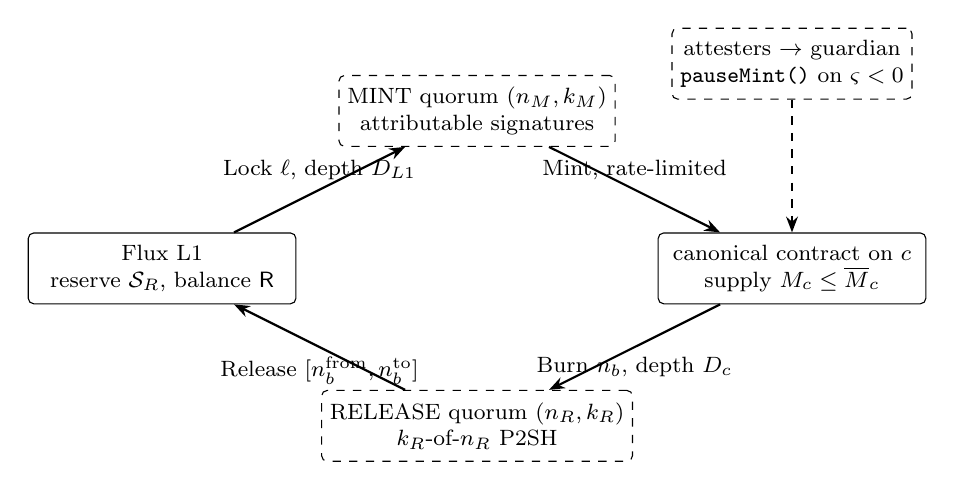
\begin{tikzpicture}[
  font=\footnotesize,
  box/.style={draw, rounded corners=2pt, align=center, minimum height=9mm, inner sep=3pt},
  ar/.style={-{Stealth[length=2mm]}, thick}
]
\node[box, minimum width=34mm] (l1) at (0,0) {\Flux L1\\reserve $\mathcal{S}_R$, balance $\mathsf{R}$};
\node[box, minimum width=34mm] (c) at (8,0) {canonical contract on $c$\\supply $M_c \le \overline{M}_c$};
\node[box, minimum width=26mm, dashed] (q) at (4,2.0) {MINT quorum $(n_M,k_M)$\\attributable signatures};
\node[box, minimum width=26mm, dashed] (r) at (4,-2.0) {RELEASE quorum $(n_R,k_R)$\\$k_R$-of-$n_R$ P2SH};
\node[box, minimum width=30mm, dashed] (att) at (8,2.6) {attesters $\to$ guardian\\\texttt{pauseMint()} on $\varsigma<0$};
\draw[ar] (l1) -- node[above, pos=0.5]{Lock $\ell$, depth $D_{L1}$} (q);
\draw[ar] (q) -- node[above, pos=0.5]{Mint, rate-limited} (c);
\draw[ar] (c) -- node[below, pos=0.5]{Burn $n_b$, depth $D_c$} (r);
\draw[ar] (r) -- node[below, pos=0.5]{Release $[n_b^{\mathrm{from}},n_b^{\mathrm{to}}]$} (l1);
\draw[ar, dashed] (att) -- (c);
\end{tikzpicture}
\caption{The two directions of \Cref{con:bridge}. Burn is permissionless and never pausable; mint is
capped, rate-limited and pausable. \planned}
\label{fig:bridge-cycle}
\end{figure}

\paragraph{The decided constants.} \Cref{tab:bridge-decided} fixes the parameters on which every
quantitative claim in this section turns. All nine are decisions, not findings; the provenance is
three intake rounds and the paper carries no independent confirmation of any of them. \planned

\begin{table}[H]
\centering\footnotesize
\begin{tabular}{@{}llp{6.0cm}@{}}
\toprule
parameter & decided value & enforcement point \\
\midrule
$\bcap{c}$ & \num{250000000}\flux & contract constant on each $c$, checked on every mint path; the global \num{560000000}\flux{} cap is enforced by the reserve under honest-minority operation, not here (\Cref{rem:global-cap}) \\
$\varrho_c$ & \num{10000000}\flux \emph{per chain} & leaky bucket inside each contract, Algorithm~\ref{alg:mint} \\
$\varrho^{\mathrm{burn}}_c$ & \num{10000000}\flux \emph{per chain} & second bucket on the burn path (\Cref{rem:burn-ceiling}) \\
$T_{\mathrm{win}}$ & \SI{24}{\hour} & leaky-bucket drain interval for both buckets \\
$(n_M,k_M) = (n_R,k_R) = (n_A,k_A)$ & $(4,3)$ & one signer set for all three, the four named co-founders \\
$\mathcal{G}$ & the same four, \textbf{1-of-4} & any single member pauses mint for $\le \Delta_g$ (\Cref{cor:pause}), or cancels a queued admin action or upgrade \srcintent{08-answers-round-2.md, round 18} \\
limit adjustability & none & $\varrho_c$, $\varrho^{\mathrm{burn}}_c$ fixed at deployment \\
upgrade path & \textbf{present}, under $(4,3)$, behind $\Delta_A = \qty{48}{\hour}$ & admin quorum may replace contract code after a \qty{48}{\hour} public queue (\Cref{rem:upgrade-voids}, \Cref{rem:timelock-decided}) \\
premine & $0$ on every $c$ & no constructor mint; $M_c$ begins at zero \\
\bottomrule
\end{tabular}
\caption{Decided bridge parameters \srcintent{08-answers-round-2.md, rounds 5--7}. The quorum figures
supersede the $(n,k)$ recommendations that \Cref{as:admin} previously carried as open. The guardian
row is no longer marked for confirmation: the pause is decided at 1-of-4, which is what makes
\Cref{prop:worst-case} a bound rather than a restatement of the cap. The last two rows are in
tension with each other --- limits that cannot be adjusted sit inside code that can be replaced ---
and \Cref{rem:upgrade-voids} is where that tension is resolved or not. \planned}
\label{tab:bridge-decided}
\end{table}

\paragraph{Why the limit is per chain and not per address, which is the team's argument and is
correct.}
A per-address mint limit is not a limit. Addresses on every $c \in \mathcal{C}$ are free to create:
an EVM address is the hash of a locally generated public key and costs nothing to produce, so an
adversary subject to a limit of $x$ per address obtains $nx$ by naming $n$ recipients, at the cost of
$n$ transactions and nothing else \srcintent{08-answers-round-2.md, round 5} \srcinferred. Nothing in
the Lock memo or the MintAuth digest of \Cref{con:bridge} binds \texttt{recipient} to an identity, and
no such binding is available on any chain in $\mathcal{C}$ without an identity registry the design
does not have and does not want. A rate control is only a control when the resource it meters cannot
be manufactured by the party being metered; the bucket in Algorithm~\ref{alg:mint} meters issuance
itself, which cannot be. The same reasoning rules out a per-lock or per-transaction ceiling, which an
adversary splits the same way.

\paragraph{Where the limit is enforced, and why a per-chain limit makes that question disappear.}
The contracts are one per chain and cannot read each other's storage, so a limit defined over
$\sum_{c} M_c$ would have no single enforcement point: it could only be a signing policy the mint
quorum observes voluntarily, which bounds nothing in the case the limit exists for, since the party
applying the policy is by hypothesis the compromised party. \textbf{The decision removes that
problem rather than solving it.} $\varrho_c$ is a per-chain constant, and a statement about chain
$c$'s own issuance over $c$'s own clock is exactly what $c$'s contract can check about itself. The
bound therefore holds \emph{under quorum compromise}, because the contract applies it whatever the
signatures say, and no allocation of a shared budget across $\mathcal{C}$ has to be decided,
enforced or revisited. Two consequences are worth naming. Honest throughput is $|\mathcal{C}|
\varrho_c$ rather than a shared $\varrho$, so capacity does not have to be predicted per market ---
which was the operational argument against a fixed split. And the adversary's bound scales the same
way: it is additive in the number of live chains (\Cref{prop:worst-case}), so \emph{adding a chain
raises the worst case by \num{10000000}\flux per reaction window}, which makes chain count a security
parameter and not only a product decision.

\paragraph{No premine, and why that makes the cap unreachable by honest use.} The legacy EVM tokens
were created by minting \num{440000000}\flux to the deployer in the constructor
\srccode{flux-eth-bsc/\allowbreak{}flux.sol}{6--13}. The canonical contracts mint nothing at construction, so
$M_c = 0$ at deployment and every unit on $c$ traces to a specific L1 lock or to a migration deposit
(\Cref{def:canonical}, H2). Combined with \Cref{thm:reserve-dominance} this has a consequence worth
stating: honest issuance is bounded by the reserve, $\sum_c M_c \le \mathsf{R}$, and $\mathsf{R}$
cannot exceed issued main-chain supply, which was \num{429466823.97}\flux at height \num{2912015}
\srcmeasured{emission model, observed mode}{2026-09-03} (\Cref{sec:app-emission}). The cap of
\num{560000000}\flux --- global, and enforced by \Cref{thm:reserve-dominance} rather than by a
contract constant (\Cref{rem:global-cap}) --- therefore cannot bind on any honest path for as long as
issued supply is below it. On the deployed schedule that is the early 2050s: issued supply reaches \num{548043625.86}\flux
at the end of \PoN year 20 (height \num{24095199}, approximately 2046-10) and then grows at a
constant \num{1789219.274256}\flux per year, so \num{560000000}\flux is first issued about
$\num{11956374}/\num{1789219} \approx 6.7$ years later, in 2053 \srcinferred
(\Cref{sec:app-emission}). Only the per-chain constant $\bcap{c}$ binds on the unbacked path, and it
is reached in \SI{25}{\day} at the permitted rate. That is the precise sense in which the cap is a backstop and not
a bound.

\SetKwInput{KwBrInv}{Invariant}
\SetKwInput{KwBrFail}{Failure mode}

\begin{algorithm}[H]
\caption{Contract-side admission of \texttt{mint} on chain $c$. \planned}
\label{alg:mint}
\KwIn{$(\ell, v, \mathrm{recipient}, \mathrm{sigs}[])$; contract state of \Cref{con:bridge}; wall
clock \texttt{now}.}
\KwOut{$v' = v - \varphi_{\mathrm{mint}}$ minted to \texttt{recipient}, or revert.}
\KwBrInv{On any successful return: $M_c \le \overline{M}_c$, $\ell \in \mathsf{used}_c$ once
$\mathsf{rem}_c[\ell] = 0$, $\mathsf{bucket}_c \le \varrho_c$, and $\mathsf{cumMint}_c$ increased by
exactly $u$.}
\KwBrFail{Revert. Execution on $c$ is atomic per transaction, so no partial state change is
possible; the caller may resubmit. No off-chain record is written anywhere (H9).}
\BlankLine
\lIf{$\mathrm{now} < \mathsf{pausedUntil}$}{\Return revert (paused)}
$S \leftarrow$ the set of distinct members of $Q_M$ with a valid signature in $\mathrm{sigs}[]$ over
the MintAuth digest for \emph{this} chain identifier and \emph{this} contract address\;
\lIf{$|S| < k_M$}{\Return revert (quorum)}
\lIf{$\ell \in \mathsf{used}_c$}{\Return revert (lock fully consumed)}
$v' \leftarrow \mathsf{rem}_c[\ell]$ if set, else $v - \varphi_{\mathrm{mint}}$
\tcp*{unminted remainder of a pending lock}
\lIf{$v' \le 0$ \textbf{or} $v < v_{\min}$}{\Return revert (dust)}
$\mathsf{bucket}_c \leftarrow \max\!\big(0,\ \mathsf{bucket}_c - \varrho_c \cdot \Delta t / T_{\mathrm{win}}\big)$
\tcp*{leak since last update}
$u \leftarrow \min\!\big(v',\ \overline{M}_c - M_c,\ \varrho_c - \mathsf{bucket}_c\big)$
\tcp*{admissible now}
\lIf{$u \le 0$}{\Return revert (cap or rate limit; $\ell$ stays pending)}
$\mathsf{rem}_c[\ell] \leftarrow v' - u$;\quad
\lIf{$\mathsf{rem}_c[\ell] = 0$}{$\mathsf{used}_c \leftarrow \mathsf{used}_c \cup \{\ell\}$}
$\mathsf{bucket}_c \mathrel{+}= u$;\quad
$\mathsf{cumMint}_c \mathrel{+}= u$\;
mint $u$ to \texttt{recipient}\;
\end{algorithm}

\paragraph{Why a sliding window and not an epoch counter.} The bucket in
Algorithm~\ref{alg:mint} drains linearly over $T_{\mathrm{win}}$ rather than resetting at fixed epoch
boundaries. With fixed epochs, an adversary who times a compromise at a boundary obtains
$2\varrho_c$ instantly, before any reaction is possible; with a sliding window the total admitted over
an interval of length $T$ is the headroom left in the bucket at the start plus the leak over $T$,
which is at most $\varrho_c(1 + T/T_{\mathrm{win}})$ and is the accounting
\Cref{prop:worst-case} rests on \srcinferred. This is the same class of timing attack that a
deterministic payout schedule admits, and the leaky bucket removes it.

\paragraph{The mint path in full.} A holder broadcasts a Lock. Each mint-quorum signer, from
\emph{its own} L1 node rather than a shared RPC, waits until the lock is at depth $\ge D_{L1}$. The
floor is $D_{L1} \ge 40 = \texttt{MAX\_REORG\_LENGTH}$ \srccode{fluxd/\allowbreak{}src/\allowbreak{}main.h}{74}, because a
reorganisation deeper than 40 blocks is rejected by consensus and the lock is then irreversible for
every node following the rules; at the \PoN target spacing this is
$40 \times \SI{30}{\second} = \SI{20}{\minute}$ \srcinferred. The signer checks memo
well-formedness, that $o_1$ is the only reserve output, and that $\ell \notin \mathsf{used}_c$ read
from its own node on $c$, then publishes its signature. Anyone may then submit the mint; the fee
$\varphi_{\mathrm{mint}}$ was locked and never minted, so it remains in $\mathsf{R}$ as surplus and
requires no fee key. A lock whose value exceeds the bucket's headroom --- including any single lock
above $\varrho_c$ --- is neither refused nor refunded: it stays pending and is minted in instalments
across successive windows, and no admin refund power exists
\srcintent{08-answers-round-2.md, round 18}. Algorithm~\ref{alg:mint} is written for the whole-lock
case; the instalment form keeps an unminted remainder per $\ell$ in place of the binary
$\mathsf{used}_c$ and admits $\min(v',\ \varrho_c - \mathsf{bucket}_c,\ \bcap{c} - M_c)$ per call,
and every bound below is unchanged by it because each instalment passes the same tests.
\settlednote{$D_{L1} = \num{40}$ (\Cref{tab:22-recommended}). $D_{L1} \ge 40$ blocks. Raising it above 40 adds latency and buys nothing against the
2-of-4 emergency-block path \srccode{fluxd/\allowbreak{}src/\allowbreak{}emergencyblock.cpp}{183--191}, which bypasses
eligibility but not the reorg limit. Trade-off: user-visible mint latency against nothing;
40 is both the floor and the chosen value: it is exactly the consensus reorg bound, and exceeding it buys nothing.}
\settlednote{$v_{\min} = \num{10}\flux$, $\varphi_{\mathrm{mint}} = 0$, $\varphi_{\mathrm{rel}} =$ the batch's gas share, recipient Foundation operations (\Cref{tab:22-recommended}). $v_{\min}$ and the fee schedule $(\varphi_{\mathrm{mint}}, \varphi_{\mathrm{rel}})$, plus
the fee recipient. Domain: $v_{\min} > $ L1 dust threshold $+\ \varphi_{\mathrm{rel}}$. Trade-off:
griefing resistance and release-batch size against small-holder access. Constraint: fees must not
scale a signer's income with volume that signer can itself generate.}
\settlednote{A Flux-hosted feed plus a mandatory IPFS mirror (\Cref{tab:22-recommended}). Transport for MintAuth signatures. A Flux-hosted feed is acceptable on the merits ---
signatures are self-authenticating and anyone may relay them, so the feed can withhold but cannot
forge --- but the choice of transport and whether a Flux-independent mirror is mandatory were the
open items, settled as above. Trade-off: operational simplicity against a withholding vector that delays holders who
rely on one relayer.}

\begin{algorithm}[H]
\caption{Release-batch construction, executed independently by each release signer. \planned}
\label{alg:release}
\KwIn{The burn log of chain $c$ up to depth $D_c$; the L1 release ledger for $c$; the UTXO set of
$s_{\mathrm{hot}}$; batch cadence $T_{\mathrm{rel}}$.}
\KwOut{A signature share on a Release transaction covering a contiguous nonce range, or abstention.}
\KwBrInv{The set of nonce ranges released for $c$ is pairwise disjoint and every released nonce is
$< B_c$. Value paid never exceeds $\sum_c \mathsf{cumBurn}_c$ minus what was already released.}
\KwBrFail{Fewer than $k_R$ signers sign $\Rightarrow$ the batch is not broadcast and exits
\emph{stall visibly}; no partial payment occurs and no burn is lost, because the claim remains
on-chain on $c$. A signer that detects an overlapping range abstains, which is the enforcement
point for the disjointness invariant --- the L1 does not check it. A malformed address forfeits its
own burn and blocks no other \srcintent{08-answers-round-2.md, round 18}.}
\BlankLine
$\mathcal{N} \leftarrow$ nonces $n_b$ of burns on $c$ at depth $\ge D_c$, ordered\;
$\mathsf{released}_c \leftarrow$ union of nonce ranges appearing in \texttt{FLXR1} memos for $c$ on the L1\;
$[n^{\mathrm{from}}, n^{\mathrm{to}}] \leftarrow$ the maximal contiguous prefix of
$\mathcal{N} \setminus \mathsf{released}_c$\;
\lIf{$[n^{\mathrm{from}}, n^{\mathrm{to}}] \cap \mathsf{released}_c \ne \emptyset$}{\Return abstain (double
release)}
\lIf{$n^{\mathrm{to}} \ge B_c$}{\Return abstain (nonce beyond counter)}
\ForEach{burn $j$ in the range}{
  verify \texttt{fluxAddr}$_j$ is a well-formed transparent address\;
  \lIf{malformed}{$v_j \leftarrow 0$ (the nonce stays inside the range and is paid nothing; the
  memo records it as \emph{unpayable}, so the prefix advances)}
}
choose inputs $i$ and burners $b$ subject to $34b + 401i + 60 \le \num{2000000}$ bytes
\tcp*{$\le$ \texttt{MAX\_TX\_SIZE\_AFTER\_SAPLING} at the decided 3-of-4}
\Return signature share on the resulting transaction\;
\end{algorithm}

\begin{remark}[The burn ceiling never refuses, and H5 therefore holds --- recommended, not decided]
\label{rem:burn-ceiling}
The burn ceiling $\varrho^{\mathrm{burn}}_c$ admitted two implementations that are indistinguishable
in a parameter table and are not the same object. Under a \emph{refusing} implementation
\texttt{burn} reverts once the window's bucket is full, and a holder is then prevented by a contract
rule from publishing a claim on the reserve --- which is exactly what H5 forbids, and which makes
\Cref{op:liveness} worse rather than better. Under a \emph{delaying} implementation the exit is
deferred to a later window but never refused across the sequence of windows.

\proposednote{A burn is never refused: the delaying implementation, recommended by this paper.
Round 7 decided the \num{10000000}\flux{} ceiling and not which of the two implementations carries
it \srcintent{08-answers-round-2.md, round 7}; no later round chooses, so the choice is recorded here
as a recommendation rather than a decision \srcintent{08-answers-round-2.md, round 18}. Under it H5
holds in the form \emph{no role can prevent a burn from eventually succeeding}, and whether the
implementation carries an explicit deferral queue or simply declines to rate-limit burns at all is
not consequential to any property in this section.}

The reasoning is worth recording, because it also explains why the asymmetry between the two ceilings
is correct rather than an oversight. A mint ceiling protects the reserve: it bounds how much
unbacked supply a compromised quorum can issue, which is the whole content of
\Cref{prop:worst-case}. A burn does the opposite --- it destroys parallel supply and strictly
\emph{improves} the conservation position of \Cref{thm:reserve-dominance}. Limiting it therefore protects
nothing while creating a liveness risk, and the risk lands at the worst possible moment: a burn
ceiling binds during a loss-of-confidence exit, which is precisely the scenario in which holders most
need the exit to work. A refusing ceiling would additionally be cheap to weaponise --- an adversary
could saturate the window with small burns to trap other holders inside it --- so the refusing
reading is not merely worse on principle, it is exploitable.
\end{remark}

\paragraph{The burn path in full.} A holder calls \texttt{burn}; no role can block it. Each release
signer waits for finality on $c$, not a confirmation count: on Ethereum the finalized checkpoint at
two epochs is $2 \times 32 \times \SI{12}{\second} = \SI{768}{\second} = \SI{12.8}{\minute}$, or
\SI{19.2}{\minute} if a third epoch is needed \srcinferred. Signers then co-sign a batch covering a
contiguous nonce range. Contiguity is what makes double-release auditable from the two public
ledgers. Sizing is a bounded, stated quantity rather than an emergent one, and the decided quorum
makes it generous: at $(n_R,k_R) = (4,3)$ the redeem script is $4 \times 34 + 3 = \num{139}$ bytes and
one P2SH input is approximately \num{401} bytes --- three signatures plus the script --- against
\texttt{MAX\_TX\_SIZE\_AFTER\_SAPLING} of \num{2000000} bytes, so one release paying roughly
\num{1000} burners in about \SI{34}{\kilo\byte} of outputs can still consume on the order of
\num{4900} reserve inputs \srcinferred. The same computation at the previously recommended 9-of-15
gave approximately \num{1215} bytes per input and roughly \num{1600} inputs; the small set costs
independence and buys transaction capacity, which is the honest way round to state the trade.
\settlednote{Each chain's own finality tag, never a confirmation count (\Cref{tab:22-recommended}). $D_{\mathrm{ETH}}, D_{\mathrm{BSC}}, D_{\mathrm{SOL}}$ must each be set \emph{at finality},
not at a confirmation count --- the latter is the error class that the BNB Bridge incident belongs
to. Ethereum's value follows from the protocol constant above; BSC's depth under fast finality and
Solana's \texttt{finalized} commitment are deploy-time parameters, set to each chain's own finality predicate rather than to a count. Trade-off:
redemption latency against reorg exposure bounded by $\mathsf{R}_{\mathrm{hot}}$.}
\settlednote{$T_{\mathrm{rel}} = \SI{4}{\hour}$ (\Cref{tab:22-recommended}). Release cadence $T_{\mathrm{rel}}$, domain $[\SI{1}{\hour}, \SI{24}{\hour}]$. Trade-off:
user-visible exit latency against batch efficiency and signer operational load.}
\settlednote{$\mathsf{R}_{\mathrm{hot}} = \num{500000}\flux$, top-up when hot ${<}\ \num{200000}\flux$ (\Cref{tab:22-recommended}). $\mathsf{R}_{\mathrm{hot}}$ target, the cold-reserve threshold, and the cold$\to$hot top-up
cadence. Domain: $\mathsf{R}_{\mathrm{hot}} \approx$ several days of expected redemption volume.
Trade-off: this quantity \emph{is} the L1-side loss bound under H4, against release latency when the
hot balance is exhausted. Sharpened by the quorum decision: the three keys that reach the mint bound
of \Cref{prop:worst-case} are the same three that reach this one, so the exposure of a single 3-key
compromise is $\mathcal{L}(T_{\mathrm{react}}) + \mathsf{R}_{\mathrm{hot}}$ and this target is a
security parameter, not only an operational one.}

\paragraph{Administration, guardianship, and the upgrade path the decision retains.} Any single
$g \in \mathcal{G}$ may call \texttt{pauseMint()}, setting
$\mathsf{pausedUntil} \leftarrow \max(\mathsf{pausedUntil}, \mathrm{now} + \Delta_g)$; the call is
attributable to $g$, and the decided rule is 1-of-4 \srcintent{08-answers-round-2.md, round 7}. The
admin quorum may extend by $\Delta_A$ per signed extension, each on-chain. Burn, transfer and
\texttt{migrate} are never paused, so a pause that is never lifted is a public, attributable,
repeatedly-renewed act by named individuals, which is the whole defence against
pause-as-censorship --- and the bounded window $\Delta_g$ is what keeps a single malicious guardian
able to stall the mint path but not to halt it, since the pause lapses unless renewed and renewal is
again public and attributable. Admin parameter changes are queued on-chain and visible for
$\Delta_A$; \emph{tightening} (lowering $\overline{M}_c$ or $\varrho_c$, removing a signer) executes
immediately, \emph{loosening} waits. Any single $g \in \mathcal{G}$ may also call
\texttt{cancel($q$)} on a queued admin action or upgrade $q$, removing it from $\mathsf{queue}$
before it executes \srcintent{08-answers-round-2.md, round 18}; the call is attributable to $g$, as
the pause is.

\textbf{The construction specifies no proxy, no \texttt{upgradeTo} and no \texttt{delegatecall} to
mutable code (D3); the decided configuration keeps an upgrade path under the same 3-of-4}
\srcintent{08-answers-round-2.md, round 7}. Under D3, replacement on EVM would be by migration:
ADMIN sets \texttt{migration\allowbreak{}Target} once, holders call \texttt{migrate(v)}, which burns on the old
contract and calls \texttt{mintMigrated} on the new one whose \texttt{predecessor} is fixed at
construction; the old contract keeps \texttt{burn} live forever, so a holder who never migrates can
still exit to the L1. The predecessor path is uncapped by $\Lambda_c$ and capped by $\bcap{c}$, and
the burn inside \texttt{migrate} takes no nonce and emits no \texttt{Burn}, so it enters no release
range \srcintent{08-answers-round-2.md, round 18}: were it a nonced burn, Algorithm~\ref{alg:release}
would pay a claim whose value had already been reissued on the successor and $\varsigma$ would go
negative. Under the decided configuration the same replacement is available without
holder action and without notice, which is convenient for repair and is the attack step of
\Cref{rem:upgrade-voids}. The two are not reconcilable by drafting; they are reconcilable only by
the timelock $\Delta_A$, and only if $\Delta_A > T_{\mathrm{react}}$.

Guardian membership at launch is decided: the same four co-founders
\srcintent{08-answers-round-2.md, round 5}, with the single-member pause of \Cref{con:bridge}
retained and now confirmed at source --- \Cref{cor:pause} shows why that retention is load-bearing
rather than incidental. $(n_A, k_A) = (4,3)$ is likewise decided, so the previously open clauses
$n_A \le n_R$ and $k_A \ge k_R$ are satisfied trivially and vacuously: they hold because the sets are
identical, which is not what they were written to secure (\Cref{rem:sets-coincide}).
\settlednote{$\Delta_g = \SI{48}{\hour}$ (\Cref{tab:22-recommended}). $\Delta_g$, domain $[\SI{6}{\hour}, \SI{7}{\day}]$. Note that $\Delta_g > T_{\mathrm{react}}$
is \emph{not} a constraint here: \Cref{prop:worst-case} needs the pause to begin, not to persist, so
what $\Delta_g$ must outlast is only the time to convene the admin quorum and decide what to do.
Trade-off: at 1-of-4 the pause is cheap to trigger by design, so $\Delta_g$ is
exactly the cost a single malicious or mistaken guardian can impose per call. Longer is a stronger
stop and a longer stall; the bound on abuse is that stalling is repeated, public and attributable,
while halting outright is not available at any $\Delta_g$.}
The parameter timelock is likewise $\qty{48}{\hour}$ (\Cref{rem:timelock-decided}), which
satisfies $\Delta_A > T_{\mathrm{react}}$ for any reaction time under two days and leaves a holder
that long to complete a burn-and-release round trip before a parameter change binds them.

\paragraph{Which multisig implementation, and why not the audited one.} On EVM the mint check would
be per-signer ECDSA verification inside the bridge contract --- a distinct-signer bitmap and
\texttt{ecrecover} against $Q_M$ --- and specifically \emph{not} the Halborn-audited Schnorr
\texttt{Multi\allowbreak{}Sig\allowbreak{}Smart\allowbreak{}Account} \srcdoc{account-abstraction/aa-schnorr-multisig-sdk/README.md:76}. Two
evidence-based reasons. First, the aggregated Schnorr signature is verified as a single combined
address, so the contract never learns \emph{which} $k$ signers participated
\srccode{account-abstraction/\allowbreak{}contracts/\allowbreak{}schnorr/\allowbreak{}Schnorr.sol}{7--26}, which defeats H3. Second, its
X-of-Y semantics are realised by enumerating every qualifying signer subset as a separate owner
address \srccode{account-abstraction/\allowbreak{}aa-schnorr-multisig-sdk/\allowbreak{}src/\allowbreak{}helpers/\allowbreak{}schnorr-helpers.ts}{129--152},
i.e.\ $\sum_{j \ge k}\binom{n}{j}$ role grants --- 29 for $(7,5)$ but \num{4944} for $(15,10)$, on the
order of \num{124e6} gas of grants at initialisation \srcinferred --- while the SDK's nonce-reuse
protection is process-local and the documented consequence of reuse is private-key exposure
\srcdoc{account-abstraction/aa-schnorr-multisig-sdk/README.md:14--16}. The Schnorr account is the
right tool for a 2-of-2 wallet and the wrong tool for a bridge quorum. On Solana, the SSP
\texttt{Solana-\allowbreak{}Multisig} program keeps \texttt{approvals:\allowbreak{} Vec<Pubkey>} on-chain and is therefore
attributable \srccode{Solana-Multisig/\allowbreak{}programs/\allowbreak{}solana-multisig/\allowbreak{}src/\allowbreak{}lib.rs}{880--918}, with the
threshold enforced at spend time \srccode{Solana-Multisig/\allowbreak{}programs/\allowbreak{}solana-multisig/\allowbreak{}src/\allowbreak{}lib.rs}{468--471};
it is a candidate for the ADMIN and upgrade authority, but only after an external audit --- none is
recorded in the corpus --- and after its own mainnet upgrade authority is moved off the single
keypair it is on today \srcdoc{Solana-Multisig/docs/MAINNET\_RUNBOOK.md:1--13}. The bridge program's
Solana mint check would verify $k_M$ Ed25519 signatures through the native Ed25519 program with
instruction introspection: precisely the code path whose sysvar check was the Wormhole vector
(\Cref{sec:bridging-incidents}), and therefore a named audit focus.

\noindent\textbf{The quorum question is closed.} $(n_M, k_M) = (n_R, k_R) = (4,3)$, one set, the four
named co-founders \srcintent{08-answers-round-2.md, round 5}. Both sets sit well inside the P2SH
ceiling --- standardness caps the redeem script at 520 bytes, which is 15 compressed keys
\srcinferred --- so the constraint that bounded $n_R$ from above is not active. The theft/censorship
trade-off resolves as follows at $(4,3)$: theft needs 3 colluders and censorship needs 2 refusers, so
the release path is easier to stall than to rob, and \Cref{op:liveness} is correspondingly wider than
it would be at a larger $n_R$. \Cref{sec:bridging-assumption} states what the shared membership costs.
\settlednote{The named hardware class and procedure of \S\ref{sec:22:recommended}. Custody standard for the four keys: dedicated signing hardware, keys never on a host
running a relayer, an RPC or the incumbent service, and a documented key-generation ceremony.
Domain: a named hardware class plus a published procedure. Trade-off: a stricter standard slows
signing and reduces the chance that one compromise of a general-purpose host yields a key --- which
under a single 3-of-4 set yields every capability at once. Note that the clauses about
\emph{organisational} distribution and jurisdictional spread are not open parameters any more; they
are not satisfied at all, and \Cref{as:admin} says so.}

\subsection{The supply invariant}
\label{sec:bridging-invariant}

\begin{theorem}[Reserve dominance]
\label{thm:reserve-dominance}
Let all quantities be read at a stated pair of heights $(\hgt, \{h_c\})$, and assume
(i) every mint on every $c$ passed the checks of Algorithm~\ref{alg:mint};
(ii) at most $k_M - 1$ mint signers and at most $k_R - 1$ release signers are corrupt on each chain;
(iii) $R_0 \ge \Lambda$ (H8); and
(iv) $V_{\mathrm{out}} = 0$, i.e.\ no reserve outflow occurs other than releases.
Then
\begin{align*}
\varsigma \;\defeq\; \mathsf{R} - \sum_{c \in \mathcal{C}} M_c
\;=\;& \underbrace{\Big(\Lambda - \sum_c \mathsf{cumMig}_c\Big)}_{\text{(1) unmigrated legacy}}
\;+\; \underbrace{\Big(V_{\mathrm{lock}} - \sum_c \mathsf{cumMint}_c - F_{\mathrm{mint}}\Big)}_{\text{(2) locks not yet minted}} \\[0.6em]
{}+\;& \underbrace{\Big(\sum_c \mathsf{cumBurn}_c - V_{\mathrm{rel}} - F_{\mathrm{rel}}\Big)}_{\text{(3) burns not yet released}}
\;+\; \underbrace{\Big((R_0 - \Lambda) + V_{\mathrm{top}} + F_{\mathrm{mint}} + F_{\mathrm{rel}} - V_{\mathrm{out}}\Big)}_{\text{(4) surplus}}
\end{align*}
and every bracket is non-negative; hence $\varsigma \ge 0$, i.e.\ $\mathsf{R} \ge \sum_c M_c$, at
every pair of heights. \planned
\end{theorem}

\begin{proof}[Proof sketch]
The contract's arithmetic admits exactly three mutators of \texttt{totalSupply}, so
$M_c = \mathsf{cumMig}_c + \mathsf{cumMint}_c - \mathsf{cumBurn}_c$. UTXO accounting over
$\mathcal{S}_R$ gives $\mathsf{R} = R_0 + V_{\mathrm{lock}} + V_{\mathrm{top}} - V_{\mathrm{rel}}
- V_{\mathrm{out}}$, where $V_{\mathrm{rel}}$ counts only value paid to burners --- fees withheld at
release never leave the reserve and are therefore counted once, in bracket~(4). Substituting and
grouping yields the displayed identity by cancellation of $\Lambda$, $F_{\mathrm{mint}}$ and
$F_{\mathrm{rel}}$.

Non-negativity, bracket by bracket. (1) The migration mint path is bounded by
$\mathsf{cumMig}_c + v \le \Lambda_c$ inside the contract, and $\sum_c \Lambda_c = \Lambda$. (2)
Each public mint consumes a distinct $\ell$ from the lock ledger and mints $v' = v -
\varphi_{\mathrm{mint}} \le v$; single-use is enforced by $\mathsf{used}_c$ under consensus on $c$,
and value correctness by the honest signer that assumption (ii) guarantees is present in any set of
$k_M$ valid signatures. (3) Each release pays a nonce range contained in $[0, B_c)$, and
disjointness is enforced by the abstention rule of Algorithm~\ref{alg:release}, which runs whenever
at least one of the $k_R$ required signers is honest --- again assumption (ii). (4) $R_0 - \Lambda
\ge 0$ by assumption (iii), $V_{\mathrm{top}} \ge 0$ and $F_\bullet \ge 0$ by construction, and
$V_{\mathrm{out}} = 0$ by assumption (iv).

Two dynamic cases. \emph{Across the migration}: bracket~(1) drains into $\sum_c M_c$ while $R_0$
stays in $\mathsf{R}$, so $\varsigma$ decreases monotonically toward the surplus and never below it.
\emph{Across a successor contract}: \texttt{migrate} burns on the predecessor and mints on the
successor within one transaction, so $\sum_c M_c$ is unchanged and $\varsigma$ is invariant; neither
leg is a nonced burn or a migration mint, so brackets~(1) and~(3) are unchanged as well.
\end{proof}

\begin{corollary}[The quiescent form, and what the roadmap says]
\label{cor:quiescent}
Write $\supply_{\mathrm{main}} \defeq \supply(\hgt) - \mathsf{R}$ for main-chain circulating supply.
In the quiescent state --- no operation in flight, migration complete
($\sum_c \mathsf{cumMig}_c = \Lambda$), surplus swept --- every bracket vanishes, so $\varsigma = 0$
and therefore $\sum_c M_c + \supply_{\mathrm{main}} = \supply(\hgt)$. That identity is the roadmap's
phrasing, ``minted supply across every chain plus main-chain supply equals total issuance''
\srcroadmap{flux-roadmap-public.md:99}. The live form is the inequality $\varsigma \ge 0$ with the
decomposition of \Cref{thm:reserve-dominance}, which is strictly more useful: it is what makes a
\emph{negative} $\varsigma$ diagnosable, because each bracket going negative names a distinct
failure --- migrator overrun, unbacked mint, unbacked release, or reserve theft --- and each is
attributable to exactly one role in \Cref{tab:bridge-roles}. \planned
\end{corollary}

\begin{algorithm}[H]
\caption{Public verification of the reserve invariant. Runnable by anyone. \planned}
\label{alg:verify}
\KwIn{A \Flux full node; one RPC endpoint per $c \in \mathcal{C}$; the published $\mathcal{S}_R$ with
redeem scripts; a chosen height pair $(\hgt, \{h_c\})$.}
\KwOut{$\varsigma$ and the four brackets of \Cref{thm:reserve-dominance}.}
\KwBrInv{The computation reads only public chain state. It requires \textbf{no} team-maintained
wallet list and no privileged endpoint.}
\KwBrFail{If any bracket is negative, report it together with the role it implicates. If an RPC is
unreachable, the run aborts rather than substituting a cached value --- a partial read must not
produce a reassuring number.}
\BlankLine
recompute each address in $\mathcal{S}_R$ from its published redeem script; abort on mismatch\;
$\mathsf{R} \leftarrow$ sum of unspent outputs to $\mathcal{S}_R$ at height $\hgt$\;
$V_{\mathrm{lock}} \leftarrow$ sum over the \texttt{FLXB1} lock ledger;\quad
$V_{\mathrm{rel}} \leftarrow$ sum paid to burners over the \texttt{FLXR1} release ledger\;
\ForEach{$c \in \mathcal{C}$}{
  read $M_c, \mathsf{cumMint}_c, \mathsf{cumMig}_c, \mathsf{cumBurn}_c, B_c$ from contract storage at
  $h_c$\;
  check the released nonce ranges for $c$ are pairwise disjoint and all $< B_c$\;
}
$\varsigma \leftarrow \mathsf{R} - \sum_c M_c$; evaluate brackets (1)--(4)\;
\Return $\varsigma$ and the brackets\;
\end{algorithm}

\paragraph{Who can verify, and why the absence of a wallet list matters.} Anyone. $\mathsf{R}$ and
the three L1 ledgers are transparent chain facts by \Cref{def:reserve}; $M_c$ and the four
cumulative counters are public contract storage on $c$. A verifier needs a \Flux full node and one
RPC endpoint per chain, and needs \emph{no} team-maintained wallet list. This is not a stylistic
point. \Cref{sec:parallel-assets} establishes that two team-maintained reserve-wallet exclusion
lists exist today and that they disagree --- neither is a superset of the other --- so any current
circulating-supply figure that nets out team reserves depends on which list the reader happens to
use. Having exactly one published $\mathcal{S}_R$, recomputable from published redeem scripts,
removes that dependency entirely. Total issuance $\supply(\hgt)$ is itself verifiable from
\texttt{gettxoutsetinfo} together with \texttt{valuePools}, with the standing caveat that ZIP-209
turnstile enforcement is compiled in but dormant
\srccode{fluxd/\allowbreak{}src/\allowbreak{}chainparams.cpp}{322--327}; note that \Cref{thm:reserve-dominance} does not
depend on that caveat, because it compares $\mathsf{R}$ against $\sum_c M_c$ and never against
$\supply(\hgt)$.

\begin{proposition}[Bounded loss under full mint-quorum compromise]
\label{prop:bounded-mint}
Drop assumption (ii) of \Cref{thm:reserve-dominance} and suppose $k_M$ or more mint signers on chain
$c$ are corrupt from time $t_0$, with a pause first effective at $t_0 + T_{\mathrm{react}}$. Write
$b_c(t) \in [0, \varrho_c]$ for the bucket fill. Then the unbacked issuance they can produce on $c$
is at most
\[
\big(\varrho_c - b_c(t_0)\big) \;+\; \varrho_c \cdot \frac{T_{\mathrm{react}}}{T_{\mathrm{win}}}
\;\le\; \varrho_c\Big(1 + \frac{T_{\mathrm{react}}}{T_{\mathrm{win}}}\Big),
\]
and at most $\bcap{c} - M_c(t_0)$ in total; every such mint is an on-chain transaction from which the
colluding signers' identities are recoverable. \planned
\end{proposition}

\begin{proof}[Proof sketch]
Algorithm~\ref{alg:mint} applies the cap and bucket checks after the quorum check and regardless of
its outcome, so no set of signatures can exceed them; corruption removes only the guarantee that a
lock exists, never the guarantee that the bounds hold. For the bucket term, every admitted mint of
$v'$ increases $b_c$ by exactly $v'$ and the only decrease is the leak at rate
$\varrho_c / T_{\mathrm{win}}$, so the total admitted over $[t_0, t_0 + T]$ equals
$b_c(t_0 + T) - b_c(t_0) + \varrho_c T / T_{\mathrm{win}}$, and $b_c(t_0+T) \le \varrho_c$ by the
admission test. Mints authorised before $t_0$ and submitted after it consume the same bucket, so they
displace rather than add to the adversary's share; the earlier phrasing ``plus in-flight
authorisations'' overstated the bound and is withdrawn. Attributability follows from per-signer
ECDSA verification against $Q_M$: the signatures are contract inputs and are therefore permanently
public.
\end{proof}

\noindent With the parameters of \Cref{tab:bridge-decided} this becomes a number, and it is the
number on which the section's security claim now rests. Two hypotheses have to be carried
explicitly, because each of them is a decision that can be taken either way and the property is
false without them.

\begin{property}[Worst-case loss of the replacement bridge]
\label{prop:worst-case}
Let $\varrho^\star \defeq \num{10000000}\flux$ be the decided per-chain mint rate limit, so
$\varrho_c = \varrho^\star$ for every $c \in \mathcal{C}$, with
$T_{\mathrm{win}} = \SI{24}{\hour}$ (\Cref{tab:bridge-decided}). Suppose the 3-of-4 quorum of
\Cref{as:admin} is compromised at $t_0$ and the adversary mints as fast as
Algorithm~\ref{alg:mint} admits on every $c$. Assume
\begin{description}
\item[(P)] a pause is first effective at $t_0 + T_{\mathrm{react}}$ with $T_{\mathrm{react}}$ finite,
  which is what the 1-of-4 guardian rule of \Cref{cor:pause} supplies; and
\item[(U)] the adversary cannot replace the contract's code inside $T_{\mathrm{react}}$, which
  requires an upgrade timelock $\Delta_A > T_{\mathrm{react}}$ (\Cref{rem:upgrade-voids}).
\end{description}
Then the unbacked issuance over $[t_0,\, t_0 + T_{\mathrm{react}}]$ is
\[
\mathcal{L}(T_{\mathrm{react}})
\;\le\;
\underbrace{|\mathcal{C}|\,\varrho^\star \cdot \frac{T_{\mathrm{react}}}{T_{\mathrm{win}}}}_{\text{sustained}}
\;+\;
\underbrace{\textstyle\sum_{c \in \mathcal{C}}\big(\varrho^\star - b_c(t_0)\big)}_{\text{headroom at } t_0,\ \le\ |\mathcal{C}|\,\varrho^\star}
\qquad\text{and}\qquad
\mathcal{L} \;\le\; \sum_{c \in \mathcal{C}}\big(\bcap{c} - M_c(t_0)\big).
\]
The sustained term is additive in the number of live chains and evaluates as in
\Cref{tab:worst-case}. The headroom term adds at most one further $|\mathcal{C}|\,\varrho^\star$ ---
\num{20000000}\flux over the launch set --- and is largest exactly when the bridge is idle at the
moment of compromise. The cap term does not bind on any chain for
$T_{\mathrm{react}} < \SI{25}{\day}$. \planned
\end{property}

\begin{proof}
Sum the per-chain bound of \Cref{prop:bounded-mint} over $c \in \mathcal{C}$ with
$\varrho_c = \varrho^\star$ on both the sustained and the headroom term; the cap bound is the check
$M_c + v' \le \bcap{c}$, which Algorithm~\ref{alg:mint} applies on every path. Hypothesis (P) is what
makes $T_{\mathrm{react}}$ a finite quantity to substitute, and \Cref{cor:pause} discharges it.
Hypothesis (U) is what makes Algorithm~\ref{alg:mint} the code that runs for the whole of
$[t_0, t_0 + T_{\mathrm{react}}]$; \Cref{prop:bounded-mint} bounds what \emph{that} algorithm admits
and says nothing about a successor contract, so without (U) the sum is over an empty set of
enforced checks. For the numbers, with $|\mathcal{C}_0| = 2$ at launch:
$2\varrho^\star \cdot (24/24) = \num{20000000}\flux$, $2\varrho^\star \cdot (48/24) =
\num{40000000}\flux$, and $3\varrho^\star \cdot (24/24) = \num{30000000}\flux$ once
$\mathcal{C}_1 = \mathcal{C}_0 \cup \{\mathrm{SOL}\}$; and
$\bcap{c} / \varrho^\star = \num{250000000}/\num{10000000} = 25$ windows of \SI{24}{\hour}, so from
an empty contract the cap on one chain is first reached at \SI{25}{\day}, which exceeds any
$T_{\mathrm{react}}$ the design contemplates \srcinferred.
\end{proof}

\begin{table}[H]
\centering\footnotesize
\begin{tabular}{@{}llr@{}}
\toprule
chains live & $T_{\mathrm{react}}$ & sustained worst-case mint \\
\midrule
$\mathcal{C}_0 = \{\mathrm{ETH}, \mathrm{BSC}\}$ (launch) & \SI{24}{\hour} & \num{20000000}\flux \\
$\mathcal{C}_0 = \{\mathrm{ETH}, \mathrm{BSC}\}$ & \SI{48}{\hour} & \num{40000000}\flux \\
$\mathcal{C}_1 = \mathcal{C}_0 \cup \{\mathrm{SOL}\}$ & \SI{24}{\hour} & \num{30000000}\flux \\
\bottomrule
\end{tabular}
\caption{The sustained term of \Cref{prop:worst-case} at the decided per-chain limit
$\varrho^\star = \num{10000000}\flux$ per \SI{24}{\hour}
\srcintent{08-answers-round-2.md, round 7}. Headroom at $t_0$ adds at most a further
$|\mathcal{C}|\,\varrho^\star$. These figures hold under hypotheses (P) and (U) and not otherwise.
\planned}
\label{tab:worst-case}
\end{table}

\begin{corollary}[The pause is reachable by a party outside any 3-key compromise]
\label{cor:pause}
\Cref{prop:worst-case} is a statement about $T_{\mathrm{react}}$, so it would be vacuous if the
adversary also held the pause. The adversary does not. The decided rule is that \texttt{pauseMint()} is a
\textbf{single-member action of $\mathcal{G}$ at $|\mathcal{G}| = 4$} --- 1-of-4, with the bounded
window $\Delta_g$ \srcintent{08-answers-round-2.md, round 7}. An adversary holding three of the four
keys therefore does not control the pause: one guardian remains able to act, and
$T_{\mathrm{react}}$ is bounded above by that member's detection-and-response time. Hypothesis (P)
of \Cref{prop:worst-case} is discharged, and the worst-case bound holds rather than collapsing to
the cap. \planned
\end{corollary}

\begin{proof}[Proof sketch]
$T_{\mathrm{react}}$ enters \Cref{prop:worst-case} only through the time at which
$\mathsf{pausedUntil}$ first exceeds \texttt{now} in Algorithm~\ref{alg:mint}. That state is written
only by \texttt{pauseMint()}, whose authorisation predicate is the guardian rule. Under the decided
single-member rule the predicate is satisfiable by any one of four keys; an adversary holding three
cannot prevent the fourth from broadcasting, because the call is a permissionless transaction on $c$
once signed, and nothing in Algorithm~\ref{alg:mint} lets a mint consume or reset
$\mathsf{pausedUntil}$. The bound is on $T_{\mathrm{react}}$ as a \emph{human} latency, not a
protocol one: the honest guardian must notice, decide and sign, which is the subject of the
paragraph after \Cref{rem:upgrade-voids}. Note what the proof does \emph{not} establish --- that the
pause holds. It expires at $\Delta_g$ unless renewed, and renewal against a compromised admin quorum
is a repeated race the guardian wins only by repeating the call.
\end{proof}

\paragraph{Why the pause is cheap and the mint is not, which is the design reason and not a
compromise.} Pausing and minting have opposite requirements. \textbf{Pausing is a safety action that
should be cheap to trigger and expensive to abuse; minting is a value-creating action that should be
expensive to trigger and is not abusable at all if the trigger holds.} A high threshold on the mint
quorum buys exactly what a high threshold is for --- more colluders needed to create value from
nothing. The same threshold on the pause buys nothing and costs the bound, because the set that must
be unable to mint is the set that would then also be able to refuse to stop. So the two thresholds
are set in opposite directions, 3-of-4 and 1-of-4, and the asymmetry is the point rather than an
inconsistency. What makes the cheap trigger tolerable is the bounded window: a single malicious or
mistaken guardian can impose $\Delta_g$ of stalled minting per call, publicly and attributably, and
cannot halt the bridge, because burn, transfer and \texttt{migrate} are never pausable (H5) and the
pause lapses on its own.

\paragraph{Why the bound is proved against quorum compromise at all, since the objection is fair.}
A reader may reasonably ask why the section spends its central property on a scenario in which three
of four named co-founders' keys are in an attacker's hands --- a bar that is high, and this section
says so. Two answers, and the section states them rather than assuming the reader shares the
premise. First, \textbf{a bound that holds only when nobody is compromised is not a security
property.} It is a description of normal operation, which the contract's ordinary behaviour already
supplies. The entire value of a rate limit is what it guarantees in the case one hopes never happens;
evaluated against an honest quorum it guarantees nothing that was in doubt. Second, \textbf{the case
is not hypothetical in this domain.} Ronin was a 5-of-9 validator compromise, and
\Cref{tab:bridge-incidents} lists it alongside other multi-signer quorums that were taken whole. The
bar being high is a real and stateable mitigation, and it is the reason the design is defensible at
launch (\Cref{sec:bridging-assumption}); it is not a reason to leave the case unmodelled. \planned

\begin{remark}[Upgradability voids the rate limit unless the upgrade is slower than the reaction]
\label{rem:upgrade-voids}
The limits are fixed at deployment and not adjustable --- and the contracts are upgradable under the
same 3-of-4 \srcintent{08-answers-round-2.md, round 7}. An adversary holding three keys is not
obliged to mint under a limit it can delete: \textbf{step one of the attack is to upgrade the
contract and remove the limit}, after which the bound of \Cref{prop:worst-case} constrains code that
is no longer running. As specified today the rate limit therefore bounds nothing under exactly the
scenario it exists to bound, and the strongest true statement available is the cap term,
$\sum_c(\bcap{c} - M_c(t_0))$ --- a quantity starting from $\bcap{c} = \num{250000000}\flux$ per
chain against a present outstanding liability of \num{223027781.21}\flux across all ten measured
legacy chains \srcmeasured{scripts/\allowbreak{}13-issuer-balances.sh}{2026-09-03}, and therefore more than an
order of magnitude weaker than \Cref{tab:worst-case}. Note that the 1-of-4 pause does not rescue
this on its own: an upgrade that removes the limit can remove the guardian rule in the same
transaction.

\textbf{The fix composes with what is already decided and costs nothing new.} Put the upgrade path
behind the admin timelock $\Delta_A$ and require
\[
\Delta_A \;>\; T_{\mathrm{react}},
\]
which is hypothesis (U). Then a malicious upgrade is queued on-chain and publicly visible before it
takes effect; the 1-of-4 pause can fire during the delay; the limit is still the code that runs for
the whole reaction window; and the rate limit binds again. The mechanism is the one the construction
already specifies for loosening parameter changes, applied to the code as well as to the constants.
Cancellation of a queued upgrade or admin change is likewise a single-member guardian action
\srcintent{08-answers-round-2.md, round 18}; without it the pause would defer the upgrade's effect
only until $\Delta_g$ lapses, the queued upgrade would execute at $t_0 + \Delta_A$ regardless, and
the bound of \Cref{prop:worst-case} would end there with $\sum_c \bcap{c}$ as the only ceiling
after it.
\textbf{Without a timelock on the upgrade path, this section can state the cap and cannot state a
worst-case bound at all}, and every figure in \Cref{tab:worst-case} is conditional on it. This was
the load-bearing open item in the bridge design; the decision follows. \planned
\begin{remark}[$\Delta_A$ decided: \qty{48}{\hour}]
\label{rem:timelock-decided}
The upgrade timelock is set at $\Delta_A = \qty{48}{\hour}$, with upgrades remaining $3$-of-$4$
\srcintent{evidence/design/08-answers-round-2.md}. Unanimity was considered and rejected for a
reason worth recording, because it is the opposite of the one that first suggests itself: $4$-of-$4$
would indeed prevent an adversary holding three keys from upgrading, but it has no fault tolerance
at all --- a single lost, destroyed or unavailable key would make the contract permanently
unupgradable, converting a key-theft risk into a key-loss risk, and for signer sets this small key
loss is the more common failure. The recovery path from that state is a fresh deployment and another
migration, which is precisely the event upgradability exists to avoid.

\textbf{Upgradability is a bring-up mechanism with immutability as its stated destination.} The
team's reasoning for keeping it, and for keeping the quorum at 3-of-4, is that a management path is a
safety net while the system is being verified to work without bugs, and that ``it's easier to upgrade
contract rather than releasing a new one and doing migration''; as the network evolves the intent is
to move to non-upgradable contracts and automate what the quorum does today
\srcintent{08-answers-round-2.md, round 11} (\vision). The paper records this because it changes what
the trust assumption \emph{is}: not a permanent property of the design, but an explicitly temporary
one whose removal is intended and undated.

That framing is coherent, and the honest statement of its weakness is a matter of sequencing rather
than of principle. An upgradable contract under a 3-of-4 quorum is, for as long as it lasts, a
contract whose rules those three signers can rewrite --- the \SI{48}{\hour} timelock bounds the speed
of that rewrite, not its scope (\S\ref{sec:bridging-assumption}). A commitment to eventual immutability
constrains nothing until it has a trigger, and none is stated: no value threshold, no elapsed-time
condition, no audit milestone. \Cref{tab:22-recommended} does not assign one, because a date the
team has not chosen would be an invention. What the paper can say is what a trigger would need to
look like --- a published condition, checkable by a third party, after which the upgrade path is
renounced on chain --- and that until such a condition exists, the bridge should be described as
administered rather than trust-minimized, which is how \S\ref{sec:bridging-assumption} describes it.
\paragraph{The renunciation trigger: stated in shape, proposed here in checkable form.} Two
preconditions for locking immutability are settled: a \textbf{third-party security audit}, and a
\textbf{proven operating record across edge scenarios --- chain reorganizations named explicitly}
\srcintent{08-answers-round-2.md, round 12} (\planned). Separately, the team states that code will
primarily be written and audited using state-of-the-art AI models, with the third-party audit as an
additional and distinct requirement rather than a substitute
\srcintent{08-answers-round-2.md, round 12}. The paper records that as the stated development
practice; it is a claim about process, and this document takes no position on the assurance it
provides, which is why the separate third-party requirement is the load-bearing one here.

Both preconditions are the right ones, and neither is yet a trigger, because a trigger has to be
checkable by someone who does not work on the project. ``A proven time record'' is not falsifiable
without a duration, and --- more importantly --- \textbf{elapsed time proves nothing on a bridge
nobody uses}. A contract that sits idle for a year has demonstrated nothing about its behaviour
under load, under reorganization, or under an adversary; it has demonstrated only that it was idle.
Any time-based condition therefore needs a volume condition beside it, or it can be satisfied by
inactivity. The following formulation is this paper's proposal, chosen so that every clause is
verifiable from public data:

\begin{enumerate}
  \item \textbf{Audit.} A third-party security audit of the \emph{deployed bytecode} --- not of a
  source tree that was later modified --- published in full, with every critical and high finding
  either resolved in a deployed upgrade or publicly accepted with reasoning.
  \item \textbf{Duration.} At least \num{1051200} L1 blocks ($\approx$ 12 months at the
  \SI{30}{\second} target) of continuous mainnet operation \emph{after} the audit's publication.
  \item \textbf{Exercise.} Cumulative bridged volume over that period of at least
  \num{10000000}\flux{} --- one day of a single chain's rate limit, and enough that the record reflects
  use rather than idleness.
  \item \textbf{Clean record.} Within that period: zero emergency pauses invoked, and zero upgrades
  executed to correct a contract defect. Upgrades for unrelated feature work do not reset the clock;
  an upgrade fixing a correctness bug does, because the record being demonstrated is precisely that
  no such bug remains.
  \item \textbf{Reorganization evidence.} A published log of reorganizations observed on each
  connected chain during the period, with the deepest handled on each, demonstrating that the
  finality parameters of \Cref{tab:22-recommended} were exercised rather than merely configured.
  \item \textbf{Renunciation on chain.} The upgrade path is then removed by transaction --- the
  admin role renounced, not merely unused --- so that the change is verifiable by reading the
  contract rather than by trusting a statement about it.
\end{enumerate}

Clause~5 is the one that speaks directly to the stated concern, and it is also the one most likely to
be unsatisfiable on schedule: reorganizations on the connected chains are not events the project can
schedule, and a quiet year produces no evidence. If the record is thin when the other clauses are
met, the honest options are to wait or to state that the reorganization evidence is absent --- not to
treat silence as proof.

\proposednote{The six renunciation criteria above are this paper's construction. What is settled
is their \emph{shape}: a third-party security audit plus a proven operating record across edge
scenarios including chain reorganizations \srcintent{08-answers-round-2.md, round 12}. The
quantities --- twelve months, \num{10000000}\flux{} of cumulative volume, zero defect-fixing upgrades
--- are proposed so that the stated shape becomes checkable by a third party rather than asserted;
they can be changed without changing the shape. One element is a design point rather than a number and
should not be dropped when the numbers are revised: renunciation must be executed \emph{on chain}, by
removing the admin role, so that it is verifiable by reading the contract rather than by trusting a
statement about it.}

At \qty{48}{\hour} the hypothesis (U) of \Cref{prop:worst-case} is discharged for any
$T_{\mathrm{react}} < \qty{48}{\hour}$, and the value sits at the low end of the interval this
specification gave, matching common practice for governance timelocks. Two consequences follow and
neither is enforced by code, so both are stated as conditions rather than assumed.

\emph{First, the timelock bounds the attack only if the upgrade queue is watched.} A malicious
upgrade announced and unnoticed for \qty{48}{\hour} takes effect, the rate limit is deleted, and the
loss reverts to being bounded only by the cap. Monitoring the queue is therefore a security control
of the same standing as $T_{\mathrm{react}}$, not an operational nicety.

\emph{Second, \qty{48}{\hour} is sized for the bound rather than for notice.} A timelock does two
jobs: it bounds a compromise, and it gives holders time to exit before a rule change binds them. Two
days is adequate for the first and thin for the second on a bridge carrying a nine-figure balance ---
a holder who does not look over a weekend misses the window entirely. A longer delay on changes that
affect holders, with \qty{48}{\hour} retained for security fixes, would serve both; the paper notes
this once and does not press it.
\end{remark}
\end{remark}

\paragraph{$T_{\mathrm{react}}$ is now the most important operational parameter in the bridge, and
this is not obvious from the construction.} $\mathcal{L}$ is linear in $T_{\mathrm{react}}$ with
slope $|\mathcal{C}|\,\varrho^\star / T_{\mathrm{win}}$, so over the launch set every hour of
detection-and-response latency is worth $2 \times \num{10000000}\flux / 24 \approx
\num{833333}\flux$, rising to approximately \num{1250000}\flux per hour once Solana is live
\srcinferred. Three things change that slope and the design should be read as choosing among them:
the number of live chains, the per-chain limit, and $T_{\mathrm{react}}$ itself. Several things
that look as though they should do not. The cap does not: it is \SI{25}{\day} away. The quorum does
not: it is compromised by hypothesis. The audit does not: \Cref{prop:worst-case} assumes the
contract behaves as specified, and an audit is what makes that assumption true rather than what
makes the loss smaller. Reserve custody does not, because the mint side never touches $\mathsf{R}$.
What does compress $T_{\mathrm{react}}$ is monitoring cadence,
alert routing, who is on call, whether a guardian key is reachable at 03:00 local time, and how long
a human takes to believe an alarm --- none of which are contract parameters and all of which are the
operational questions this bound turns into first-order security questions. The attestation link of
\Cref{sec:bridging-attestation} exists to compress $T_{\mathrm{react}}$, and its fail-closed silence
timeout $T_{\mathrm{silence}}$ is the mechanism that puts a ceiling on it without a human in the loop.
\planned

\begin{proposition}[Dominance over the incumbent, H0, with a number on one side]
\label{prop:dominance}
Under \Cref{tab:bridge-decided} and hypotheses (P) and (U) of \Cref{prop:worst-case}, the
replacement's worst-case loss over a reaction window is $\mathcal{L}(T_{\mathrm{react}})$, which is
\num{20000000}\flux over the launch set at $T_{\mathrm{react}} = \SI{24}{\hour}$ --- a quantity fixed
by contract constants before any compromise occurs, and the same for every compromise class that can
reach the mint path, since
Algorithm~\ref{alg:mint} applies the bucket regardless of which signatures it saw. The other
directions are bounded separately and also in advance: the release side by
$\mathsf{R}_{\mathrm{hot}}$, and the guardian and relayer roles by nothing they can move. Every
bound-consuming event is a public
transaction that Algorithm~\ref{alg:verify} reads, so H0(ii) is satisfied with $T_{\mathrm{react}}$
as the stated observability bound. The incumbent's corresponding worst case is the entire balance
held under 32 single-signature hot keys across eleven chains at the moment of compromise
\srccode{fusion/\allowbreak{}config/\allowbreak{}default.js}{342--482}: a quantity fixed by nobody, published nowhere, and
detectable only by an operator reading its own records, since an unauthorised outgoing transfer from
a hot wallet is indistinguishable on-chain from an authorised one. \planned
\end{proposition}

\begin{proof}[Proof sketch]
The replacement half is \Cref{prop:worst-case} for the mint direction, the hot/cold custody split for
the release direction, and \Cref{tab:bridge-roles} for the remaining roles, none of which can mint,
transfer or freeze. The observability half follows because each bound-consuming event is a
transaction on a public chain and Algorithm~\ref{alg:verify} reads exactly those transactions from
public state, with no team-maintained list. The incumbent half is \Cref{sec:bridging-incumbent}:
single-key in-process signing on all eleven chains, with every gate --- amount ceiling, blacklist,
rate limit --- enforced in the same process that holds the keys
\srccode{fusion/\allowbreak{}src/\allowbreak{}services/\allowbreak{}swapService.js}{150--157} \srccode{fusion/\allowbreak{}src/\allowbreak{}lib/\allowbreak{}server.js}{29,38}.
\end{proof}

\noindent\textbf{What the comparison is, stated exactly.} H0(ii) is met outright: a stated
$T_{\mathrm{react}}$ (\SI{24}{\hour}, \Cref{tab:22-recommended}) against no detection bound at all. H0(i) is met in the form that matters --- a
finite bound fixed in advance against an exposure bounded by nothing in the design --- and this is
the substantive change from earlier drafts, which could state only the shape of the bound and not its
value. It is \emph{not} a comparison of two measured numbers, because the incumbent's side has never
been measured.
\notestablished{the incumbent's current hot-wallet balances across the 32 keys are not in
the evidence corpus. \Cref{prop:dominance} therefore compares a stated finite bound against an
unbounded exposure. Should that balance ever be measured and found below
$\mathcal{L}(T_{\mathrm{react}})$, H0(i) would need restating in per-window rather than absolute
terms; the measurement is a prerequisite task, not a paper gap.}

\subsection{The attestation link}
\label{sec:bridging-attestation}

\begin{definition}[Attestation]
\label{def:attestation}
An attestation is the tuple
\begin{multline*}
\mathsf{A} = \big(\hgt,\ \mathrm{hash}_{L1}(\hgt),\ \mathsf{R}_{\mathrm{hot}},\ \mathsf{R}_{\mathrm{cold}}, \\
\{(c, h_c, \mathrm{hash}_c(h_c), M_c, \mathsf{cumMint}_c, \mathsf{cumMig}_c, \mathsf{cumBurn}_c, B_c)\}_{c \in \mathcal{C}}, \\
V_{\mathrm{lock}},\ V_{\mathrm{rel}},\ \varsigma,\ \mathsf{flags}\big)
\end{multline*}
signed by attester $j$ as $\mathrm{Sign}_{sk_j}\!\big(H(\texttt{"FLXATT1"} \| \mathsf{A})\big)$.
Every field is an objective chain fact at a stated height --- the roadmap's ``states they observed''
category \srcroadmap{flux-roadmap-public.md:135--136} --- so a false attestation is provably false to
anyone holding the relevant block. $\mathsf{flags}$ carries the signer's verdicts on the two policy
invariants the L1 cannot enforce: that every \texttt{FLXR1} range is disjoint and below $B_c$, and
that every release corresponds to a burn at depth $\ge D_c$. An attestation is \emph{valid} when
$\ge k_{\mathrm{att}}$ distinct bonded attesters sign the same $\mathsf{A}$. \planned
\end{definition}

\paragraph{Where it lives, and the cost finding that decides it.} Attestations would be published
off-chain on a public feed, with only the \emph{consequence} on-chain. Posting every attestation to
Ethereum is not viable: at one attestation per L1 block, \num{2880} per day, and
$k_{\mathrm{att}} = 9$ signatures each, the cost is approximately \num{346e6} gas per day ---
between eight and twelve Ethereum blocks' worth of gas daily for one bridge's bookkeeping
\srcinferred. At $k_{\mathrm{att}} = 5$ it is \num{276e6} and at $15$ it is \num{449e6}. The
on-chain component is therefore a single guardian contract, \texttt{Attester\allowbreak{}Guardian}, one per
chain, added to $\mathcal{G}$ alongside the four named guardians of \Cref{tab:bridge-decided} once
the attestation network exists --- which is exactly the D4 transfer path, and the only mechanism in
the design by which pause authority reaches a party outside the four: it stores the attester key set
and $k_{\mathrm{att}}$, and
exposes \texttt{pause\allowbreak{}On\allowbreak{}Attestation(A, sigs[])}, which pauses mint if and only if the signatures are
valid and $\mathsf{A}$ asserts $\varsigma < 0$ or a false policy flag. It would additionally
\emph{fail closed on silence}: if no valid attestation is submitted within $T_{\mathrm{silence}}$,
the guardian pauses mint for $\Delta_g$. That direction is deliberate. The deployed \SAS watchdog
fails \emph{open} on hash-service outage --- if both hash endpoints are unreachable it treats the
node as secure and does nothing \srccode{fluxsas/\allowbreak{}src/\allowbreak{}watchdog.h}{566--596} --- and under the team
constraint an attester outage should stop issuance rather than continue it. Burn is unaffected in
either case, so the degraded bridge is exit-only, which is the correct degradation.
\settlednote{$T_{\mathrm{att}} = \num{120}$ blocks, $T_{\mathrm{silence}} = \SI{6}{\hour}$, fail-closed adopted (\Cref{tab:22-recommended}). $T_{\mathrm{att}}$ (natural domain: one attestation per L1 block, \num{2880} per day, down
to one per hour), $T_{\mathrm{silence}}$, and whether fail-closed is adopted. Trade-off: a shorter
cadence and a shorter silence timeout detect faster and make an availability failure of the feed
into a liveness failure of the bridge.}
\settlednote{The independent mirror is mandatory (\Cref{tab:22-recommended}). The feed itself and whether a Flux-independent mirror is mandatory. IPFS is the precedent
the project already uses for parameter distribution
\srccode{fluxd/\allowbreak{}zcutil/\allowbreak{}fetch-params.sh}{17}. Trade-off: a single Flux-operated feed can withhold
but not forge; an independent mirror removes the withholding vector at operational cost.}

\paragraph{Detecting a false attestation, and what the bond is at risk for.} A false attestation is
one whose fields do not match the canonical chains at the stated heights, or whose flags assert a
policy invariant the ledgers contradict. Detection is by any party running Algorithm~\ref{alg:verify}
--- the same computation, no privileged access --- and the proof of falsity is the relevant block
header plus a Merkle inclusion or storage proof for the contradicting value. Equivocation, meaning
two different $\mathsf{A}$ for the same heights, is proven by the two signatures alone and needs no
chain data. The bond $\beta_{\mathrm{att}}$ would be at risk for signing a false $\mathsf{A}$, for
equivocation, and (minor, to keep the set honest) for sustained non-participation. The economic
condition that makes collusion unprofitable is
\begin{equation}
\label{eq:bond-condition}
k_{\mathrm{att}} \cdot \beta_{\mathrm{att}} \;>\; \varrho_c \cdot
\left\lceil \frac{T_{\mathrm{react}}}{T_{\mathrm{win}}} \right\rceil
\qquad \text{for every } c \in \mathcal{C},
\end{equation}
i.e.\ the forfeited bonds must exceed what a false ``all is well'' can cover for, which is exactly
the bound of \Cref{prop:bounded-mint}.

\medskip
\noindent\textbf{The decided rate limit makes \eqref{eq:bond-condition} very expensive, and this is
worth stating rather than discovering later.} The condition is per chain, so the per-chain limit
decision leaves it unchanged in form and in magnitude: substituting
$\varrho_c = \varrho^\star = \num{10000000}\flux$ and
$T_{\mathrm{react}} = T_{\mathrm{win}} = \SI{24}{\hour}$ gives
$k_{\mathrm{att}} \cdot \beta_{\mathrm{att}} > \num{10000000}\flux$. Using the deployed Stratus tier
collateral of \num{40000}\flux purely as a yardstick and not as a recommendation, that is
$k_{\mathrm{att}} > 250$ bonded attesters --- against $k_{\mathrm{att}} = 9$, which would put only
\num{360000}\flux at risk, short of the condition by a factor of about 28 \srcinferred. Three
responses exist and the design does not yet choose between them: raise $\beta_{\mathrm{att}}$, which
concentrates the attester set and is the failure the network exists to avoid; lower $\varrho^\star$,
which lowers the bound of \Cref{prop:worst-case} and the honest throughput ceiling together; or
accept that
the attester layer is a \emph{detector} that compresses $T_{\mathrm{react}}$ rather than a
\emph{deterrent} that makes collusion unprofitable, and say so. The third is the honest description
of any attester set small enough to operate, and it is consistent with the fail-closed pause being
the attesters' only on-chain power. \planned
\notestablished{$(n_{\mathrm{att}}, k_{\mathrm{att}})$ --- the size and threshold of the attester
set. Round 23's ruling that nothing is ever slashed changes the character of this gap rather than
merely deferring it. $\beta_{\mathrm{att}}$ is \emph{void}: a bond that cannot be forfeited is a
deposit, so there is no bond to size, and \eqref{eq:bond-condition} is withdrawn rather than left
unparameterised. What remains is an ordinary quorum choice over an accountability-based attester set
--- how many named attesters, and how many must agree --- undetermined because nobody has picked the
numbers, not because the construction is unsolved. That is a materially smaller gap than this marker
previously recorded, and it closes by decision whenever the author makes one.}

\noindent The cap, the rate limit and the window are no longer open:
$\bcap{c} = \num{250000000}\flux$, $\varrho_c = \num{10000000}\flux$ per chain and
$T_{\mathrm{win}} = \SI{24}{\hour}$ (\Cref{tab:bridge-decided}). Two constraints that the open form of
those parameters carried should be checked against the decided values rather than dropped. The first,
$\bcap{c} \ge \Lambda_c$, holds with room: the measured legacy liability on the largest chain is
\num{156217342.78}\flux on Ethereum \srcmeasured{scripts/\allowbreak{}13-issuer-balances.sh}{2026-09-03}, well
below \num{250000000}\flux. The second, $\varrho_c \ll \bcap{c}$, holds at exactly a factor of 25 and
is what makes \Cref{prop:worst-case}'s cap term inactive.

\begin{remark}[The \num{560000000}\flux{} cap is global, and no contract can enforce it]
\label{rem:global-cap}
This paper read \num{560000000}\flux{} as a per-chain contract constant $\bcap{c}$, because that is
the only reading a per-chain construction can enforce by itself. That reading is wrong: the figure is
a \textbf{global cap across all chains} \srcintent{08-answers-round-2.md, round 13} (\planned).
The correction matters, because it relocates the enforcement rather than the number.

\textbf{No contract can enforce a global cap.} A contract on chain $c$ can read its own
\texttt{totalSupply} and nothing else; it cannot observe supply on the other chains or on the L1, so
it cannot evaluate the global constraint it would need to enforce. Setting $\bcap{c} =
\num{560000000}$ on every chain yields an aggregate contract-enforced ceiling of $|\mathcal{C}|
\times \num{560000000}\flux$, which for the surviving pair is \num{1120000000}\flux{} --- twice
the intended global cap. As a backstop the constant is therefore \emph{inert}: it is set far above
any level at which it could bind.

\textbf{What actually enforces the global cap is the reserve invariant.}
\Cref{thm:reserve-dominance} establishes $\mathsf{R} \ge \sum_c M_c$: minted supply on the parallel
chains is dominated by value locked on the L1, so the global total is bounded by L1 supply and cannot
exceed it however many chains exist. This is the correct and sufficient mechanism, it is already
specified, and it is exactly the mint-and-burn discipline the team describes --- ``if we mint on some
chain, another chain is burning it or locking somewhere''
\srcintent{08-answers-round-2.md, round 8}. The global cap is a property of the reserve, not of the
contracts. That holds under honest-minority operation, assumption~(ii) of the theorem; under the
quorum compromise \Cref{prop:worst-case} models, the only contract-enforced aggregate is
$\sum_c \bcap{c}$ --- \num{500000000}\flux{} at launch, \num{750000000}\flux{} with Solana --- and
$\bcap{c}$ is not lowered for that, because the guardian's cancel over queued upgrades
(\Cref{rem:upgrade-voids}) removes the path by which the aggregate was reachable
\srcintent{08-answers-round-2.md, round 18}.

\textbf{Recommendation: set $\bcap{c}$ far lower, so it is a real backstop rather than a decoration.}
A per-chain constant is genuinely useful as defence-in-depth --- it bounds the damage from a mint-path
bug or a compromised quorum on one chain, and it does so without needing cross-chain visibility. But
it only does that work if it can bind. The largest measured per-chain liability is
\num{156217342.78}\flux{} on Ethereum (\Cref{tab:issuer-liability}), so a constant of
\num{250000000}\flux{} leaves roughly \SI{60}{\percent} headroom over the largest realistic
requirement while capping single-chain damage at under half the global supply. That is this paper's
recommendation; \num{560000000} on each chain is not a cap, it is the absence of one.
\textbf{Settled at \num{250000000}\flux{}} \srcintent{08-answers-round-2.md, round 14}
(\planned): the per-chain constant binds at a level that bounds single-chain damage below half the
global supply, while leaving roughly \SI{60}{\percent} headroom over the largest measured per-chain
liability.
\end{remark}

\paragraph{The dependency, stated honestly.} An attestation network built on today's primitives
would inherit a defect that voids its central security claim, and \Cref{sec:attested-execution}
states the same finding from the other side. The \fluxsas attestation signing seed for every purpose
is derived by HKDF over salt and domain values compiled identically into every binary; none of the
inputs depends on the TPM, on Secure Boot state, or on any per-machine value
\srccode{fluxsas/\allowbreak{}src/\allowbreak{}api\_server.h}{411--481,466--469,503--506}. A signature from that key therefore
demonstrates that the signer holds a value shipped in every copy of the software. It does not
demonstrate that a particular machine observed a particular chain state. \textbf{A key that everyone
holds cannot be slashed, and a signature it produces cannot be attributed to a bond.} The
node-identity key does mix machine-derived values, but the key protecting its random component is
itself a baked-in constant \srccode{fluxsas/\allowbreak{}src/\allowbreak{}disk\_encryption.h}{200--228}. What
\Cref{sec:attested-execution} calls Requirement~0 --- per-node attester keys, generated on the node,
whose public half is committed on the L1 in the bonded-tier registration transaction so that a
signature is attributable to a specific bond outpoint --- must be met before any of
\Cref{sec:bridging-attestation} is more than a specification. The \texttt{purpose=\allowbreak{}mesh} voucher
already present in \fluxsas with no consumer \srccode{fluxsas/\allowbreak{}src/\allowbreak{}api\_server.h}{438--445} is the
natural place for such a key to land once it is per-node. Note also that the same finding applies to
the benchmark signing path, so a bonded-tier registration must not reuse it.

\begin{openproblem}[Slashing on the \Flux L1]
\label{op:slashing}
A bond held as a plain UTXO cannot be taken from its owner by consensus, and \Flux's inherited
Bitcoin script cannot express a slashing condition. The two options are (a) a consensus change
introducing a bonded-tier transaction type with a slashing rule verified by \fluxd, or (b) bonds
escrowed in a $k$-of-$n$ that adjudicates --- which reintroduces exactly the trusted quorum the
network exists to replace. This is the load-bearing hole in the attestation link. Until it is
filled, the ``bonded'' tier is a \emph{registered} tier: attributable but not slashable, and its
attestations should be weighted in $\mathcal{G}$ accordingly.
\decided{there is no slashing, here or anywhere in \Flux{}: no mechanism destroys or forfeits a
holder's \flux{} \srcintent{08-answers-round-2.md, round 23}. That closes the construction question
by removing the mechanism rather than by supplying one, and the consequence has to be carried rather
than absorbed. \textbf{An attester bond that cannot be forfeited is a deposit, not a stake}, so
\eqref{eq:bond-condition} cannot rest on it and the cryptoeconomic form of the security argument is
unavailable. What remains is accountability: a named, non-anonymous attester set whose members can be
excluded from future participation and who answer for their attestations personally, in the same
shape as the key custody of \Cref{sec:model}. That is a materially weaker claim than a bonded one,
and this paper does not dress it as equivalent --- an attester who lies loses future income and
standing, not principal, and what bounds a dishonest quorum is the rate limit and the reserve
invariant of \Cref{con:bridge}, not a forfeiture.}
\end{openproblem}

\subsection{Why not the alternatives}
\label{sec:bridging-alternatives}

\paragraph{Atomic swaps --- the question is closed, not open.} An HTLC atomic swap exchanges an
asset one party holds on chain A for an asset a counterparty holds on chain B, atomically, with no
custodian \citep{herlihy2018atomic}. \Flux's inherited script carries the primitives. But an atomic
swap cannot do what a bridge does: \textbf{it cannot issue FLUX on Ethereum}, only exchange FLUX for
something that already exists there. Everything else is secondary and still disqualifying: it
requires a counterparty holding the other asset, a discovery layer to find them, both parties online
for the duration, and it hands the initiator a free option to abort if the price moves during the
timelock. The correct conclusion is not that atomic swaps are a rejected bridge design but that they
address a different problem --- the \emph{exchange} of FLUX against ETH, USDC or another asset
against a market maker, which is \FusionX's product (\Cref{sec:bridging-incumbent}), not the
bridge's. Atomic swaps are a settled construction in the literature \citep{herlihy2018atomic}; the boundary drawn here is a product decision, not a doubt about the primitive.

\paragraph{Light-client verification --- not constructible for \Flux, and here is exactly why.} The
trust-minimizing answer would be an Ethereum contract that verifies \Flux headers directly, as IBC
does between Tendermint chains \citep{cosmosibc} and as the interoperability literature identifies as
the strongest available class \citep{zamyatin2021sok}. It is not constructible from the current
\PoN header, for three compounding reasons:

\begin{enumerate}
\item The \PoN block header carries \texttt{nodes\allowbreak{}Collateral} and \texttt{vchBlockSig} but
      \textbf{no commitment to the confirmed node set}
      \srccode{fluxd/\allowbreak{}src/\allowbreak{}primitives/\allowbreak{}block.h}{44--45,64--96}, so a verifier cannot check that a
      block's signer was eligible without the full \FluxNode registry --- which is to say, without
      being a full node.
\item Chainwork is a fixed $2^{40}$ per block regardless of difficulty target
      \srccode{fluxd/\allowbreak{}src/\allowbreak{}pow.cpp}{284--290}, so fork choice degenerates to a block-count race and
      there is no cumulative-work heuristic by which a light client could prefer one chain over
      another.
\item The 2-of-4 emergency-block path can produce a valid block outside the normal rules, with no
      time or stall-detection gating \srccode{fluxd/\allowbreak{}src/\allowbreak{}emergencyblock.cpp}{183--191}, so no
      light-client rule derived from \PoN eligibility is sound; a perfect light client would still
      be trusting those four keys.
\end{enumerate}

\noindent A future header commitment to the deterministic node list's Merkle root would reopen the
question --- after which verifying \num{2880} headers a day on Ethereum becomes a cost question, one
\texttt{ecrecover} plus a $\lceil \log_2 6489 \rceil = 13$-hash Merkle proof per header
\srcinferred --- and \Cref{sec:chain-evolution} should treat it as a candidate for the same network
upgrade that carries collateral maturity. \textbf{This is the paper's clearest instance of vertical
integration cutting both ways.} Controlling the L1 is what lets \Flux put an entitlement memo in an
\texttt{OP\_RETURN}, freeze a halving by hand, and change the reorg limit to launch \PoN; it is also
what produced a header format that forecloses the most trust-minimizing bridge architecture
available to other chains. Owning the stack does not automatically mean the stack was designed for
what you later want from it. The same tension runs through \Cref{sec:fluxos}. The reverse direction
--- \fluxd verifying Ethereum --- would need an EVM and BLS light client inside the daemon, a
consensus change of a different order.

\paragraph{Threshold-signature and MPC bridges.} One aggregate key, signed by a threshold of parties
holding shares. \emph{Trust assumption:} fewer than the threshold of share-holders collude, and the
share distribution is what it is claimed to be. \emph{Failure mode:} on-chain the contract sees a
single signer, so who participated is invisible and the claimed distribution is unfalsifiable from
outside; if the shares sit on one organisation's servers the threshold is cosmetic, which is
precisely the Multichain outcome (\Cref{sec:bridging-incidents}). \emph{Why not chosen:}
attributability is a hard requirement here (H3), and the construction additionally declines to rely
on the threshold alone --- the contract bounds the damage whatever the signing scheme. A TSS could
still be used \emph{inside} one signer organisation to protect its own key.

\paragraph{External validator sets.} A named set signs mint messages; the contract mints on
$k$ signatures. \emph{Trust assumption:} fewer than $k$ collude or are compromised.
\emph{Failure mode:} the contract does whatever $k$ signatures say, without bound --- Wormhole's 19
guardians at 13 and Ronin's 9 validators at 5 both failed this way, for different reasons.
\emph{Why not chosen, and the honest statement:} at the signing layer this construction \emph{is} a
validator-set bridge with a smaller set than either --- 4 signers at a threshold of 3, against
Wormhole's 19 at 13 and Ronin's 9 at 5 --- and pretending otherwise would be dishonest. What differs
is not the size or the independence of the set but that the cap, the per-chain rate limit, the
1-of-4 guardian pause and the admin timelock are intended to make $k$-collusion bounded and slow
rather than total and instant: \num{20000000}\flux per \SI{24}{\hour} of reaction time over the
launch set (\Cref{prop:worst-case}) instead of the pooled value. That sentence is true only under
the timelock condition of \Cref{rem:upgrade-voids}; an upgradable contract without one puts this
construction back in the same row as the systems it is being distinguished from, which is why that
item was the section's load-bearing open one until \Cref{rem:timelock-decided}. The
collateral-backed alternative in the literature --- overcollateralized vaults with automatic
liquidation \citep{zamyatin2019xclaim} --- removes the trusted set at the cost of locking capital
worth more than the bridged value on the destination chain, and of a price oracle for the
collateral-to-asset ratio. That trade is available and was not taken; the reason is that it
substitutes an oracle dependency and a capital cost for a signer dependency, and does not remove the
need for the L1-side release quorum, which is where \Cref{sec:bridging-open} shows the residual
trust actually sits.

\paragraph{Canonical rollup bridges and IBC, for completeness.} Optimism's and Arbitrum's canonical
bridges derive security from the L1 verifying the L2 through fraud or validity proofs with a
challenge window; neither \Flux nor Ethereum can verify the other, so this is not available.
Their \emph{operational} pattern --- guardian pause, security-council timelock, no silent upgrades
--- is adopted wholesale. IBC requires cheap, fast-final header verification on both ends
\citep{cosmosibc}; \Flux has neither cheap header verification nor a node-set commitment, so it is
not applicable without the header change above.

\paragraph{Issuer-attested burn-and-mint, which is the model chosen.} Circle's CCTP signs burn
messages with an issuer-operated attestation service; destination contracts mint only against
attested, nonce-bound messages, and no pooled liquidity exists to steal \citep{cctp}. Its trust
assumption is the issuer's attester key --- which, for USDC, belongs to the same party that can mint
USDC anyway, so the bridge adds no new trust. \Flux is the closest analogue and this is the chosen
model. Two differences follow from the fact that \Flux's attesters are \emph{not} already trusted for
the whole supply: an explicit $k$-of-$n$ with on-chain attribution rather than a single issuer
signature, and contract-level cap and rate limit, which CCTP does not need.

\subsection{The launch trust assumption: one quorum, bounded by a rate limit}
\label{sec:bridging-assumption}

\begin{assumption}[Single attributable quorum, bounded by contract]
\label{as:admin}
At launch the MINT, RELEASE and ADMIN authorities of \Cref{tab:bridge-roles} are held by \emph{one}
set: $n_M = n_R = n_A = 4$ and $k_M = k_R = k_A = 3$, the four keys held by the four named
co-founders --- Tadeas Kmenta, Daniel Keller, Jeremy Anderson, Valter Silva
\srcintent{08-answers-round-2.md, round 5} --- with $\mathcal{G}$ the same four individuals but at a
threshold of \textbf{one} (\Cref{tab:bridge-decided}). The assumption is that fewer than three of
those four keys are compromised or collude. It is one assumption, not four independent ones. What
supports it:
(i) each key is per-signer, so every authorisation is attributable on-chain to the key that produced
it, and the signer set is published;
(ii) each key is generated and held on dedicated signing hardware and never on a host that runs a
relayer, an RPC, or the incumbent service --- co-locating the key with the process that decides is
the incumbent's defining mistake (\Cref{sec:bridging-incumbent});
(iii) $k/n = 3/4 \ge \lceil 2n/3 \rceil / n$, so the threshold ratio is at or above the shape the
requirements recommended.
What is \emph{not} satisfied, and was written into the earlier form of this assumption precisely
because it matters: signers are named individuals rather than independent named organisations; one
organisation's founders hold every key in every set, so no clause bounding a single organisation's
share of a quorum can hold; the four memberships coincide exactly; and jurisdictional spread is
whatever those four individuals happen to have rather than a design parameter.
If the assumption fails, the contract still bounds unbacked issuance to
$\mathcal{L}(T_{\mathrm{react}})$ (\Cref{prop:worst-case}) --- the pause remains reachable at 1-of-4
(\Cref{cor:pause}), and the bound additionally requires the upgrade timelock of
\Cref{rem:upgrade-voids} --- and the L1 side to $\mathsf{R}_{\mathrm{hot}}$. \planned
\end{assumption}

\begin{remark}[The separation of powers is not available at launch, and saying otherwise would be false]
\label{rem:sets-coincide}
Three compromised keys can, in one sequence and with no second party: authorise mints up to the rate
limit; co-sign L1 spends of $\mathsf{R}_{\mathrm{hot}}$; queue an admin change raising $\bcap{c}$ and
$\varrho_c$ and replacing $Q_M$ with keys of their own; and \emph{upgrade the contract}, which
reaches every rule in \Cref{tab:bridge-roles} at once including the guardian rule
(\Cref{rem:upgrade-voids}). What they cannot do is throw the pause on the honest guardian's behalf,
prevent that guardian from throwing it, or prevent that guardian from cancelling what they queue,
because the pause and the cancel are 1-of-4 (\Cref{cor:pause}) --- and
that single exception is what the whole quantitative claim of this section rests on. The $\Delta_A$
notice period survives for parameter changes --- an admin change is still visible for $\Delta_A$
before it executes --- but the exit it is supposed to protect runs through a release quorum
consisting of the same three keys, so a holder who burns during the notice period has a public claim
and the same adversary decides whether it is paid (\Cref{op:liveness}). The total exposure of a
3-key compromise is therefore $\mathcal{L}(T_{\mathrm{react}}) + \mathsf{R}_{\mathrm{hot}}$, with
the cold reserve as the last line and $\sum_c \bcap{c}$ as the ceiling if the upgrade path is not
timelocked or a queued upgrade is not cancelled within $\Delta_A$. This is stated as a property of
the launch configuration, not as a hypothetical: the
earlier draft of this remark described the collapse as the reason separation was a requirement, and
the configuration that has been decided is the collapsed one everywhere except the pause.
\end{remark}

\paragraph{Why this is defensible, on the team's own constraint --- and what would make it not.} The
governing constraint of this section is that \emph{a decentralized design that is exploitable is
worse than the custodial incumbent} \srcintent{03-parallel-assets.md}. Taken seriously, it settles
the launch question. A more distributed signer set would have to be assembled from parties who can be
held to their signatures; the mechanism for holding them --- a bond that can be forfeited --- does
not exist on this chain (\Cref{op:slashing}), and the attestation keys that would identify them are
today fleet-shared rather than per-node (\Cref{sec:bridging-attestation}). A fifteen-key set
recruited without either property is not obviously more decentralized than four named founders: it is
the same trust assumption spread across more people who are harder to identify and cannot be
penalised, which is the shape the Ronin and Multichain rows describe
(\Cref{tab:bridge-incidents}). Against that, the decided
configuration takes the trust concentration as given and spends its design effort on making the
consequence bounded and public: the contract refuses beyond $\varrho_c$ and $\bcap{c}$ whatever the
three keys say, and anyone can run Algorithm~\ref{alg:verify} without asking the signers for
anything. \textbf{The accurate description is a custodial bridge with contract-enforced bounds and
public verification, moving toward autonomy} --- not a decentralized bridge, and not a separation of
powers. The intent on record is explicit about the direction and about the fallback: full autonomy
afterwards, and ``if the autonomous design is not ready in time, ship 3-of-4 and take a second fork
for the autonomous bridge'' \srcintent{08-answers-round-2.md}. Two things would make the position
indefensible rather than defensible, and both are checkable. \textbf{If the upgrade path ships
without a timelock satisfying $\Delta_A > T_{\mathrm{react}}$, the bound is the cap rather than
\num{20000000}\flux, and the argument above does not survive the substitution}
(\Cref{rem:upgrade-voids}) --- the contract that ``refuses beyond $\varrho_c$ and $\bcap{c}$
whatever the three keys say'' is then a contract those same three keys can replace before it
refuses anything. And if the second fork does not follow, what is described here as a launch
configuration becomes the design, at which point the honest comparison is no longer against the
incumbent but against a competently run custodian. \planned

\paragraph{The path off the single quorum, specified as requirements because the construction is
open.} The intent is autonomy, and no design for it exists in the evidence corpus. What replaces the
3-of-4 must satisfy, at minimum: \textbf{(R1)} authorisation attributable to a set whose membership
is derivable from public chain state rather than from a published list, so that an observer can
recompute who was entitled to sign at a height; \textbf{(R2)} a penalty that can actually be applied
to a misbehaving member, which on this L1 means \Cref{op:slashing} is answered first; \textbf{(R3)}
per-member keys generated on the member's own machine, which means \Cref{sec:attested-execution}'s
Requirement~0 is met first; \textbf{(R4)} liveness under member churn, since a set derived from the
node registry changes between blocks while an L1 P2SH redeem script does not; and \textbf{(R5)} a
migration path from the 3-of-4 that does not require holders to act, which under D3 means the ADMIN
role rotating $Q_M$ and $Q_R$ rather than a contract replacement. The interfaces are already fixed by
\Cref{con:bridge} and do not change: the MintAuth digest, the $k$-of-$n$ check inside
Algorithm~\ref{alg:mint}, and the P2SH release path. \textbf{The construction that meets R1--R5 is
open}, and R2 and R4 are the binding pair on this chain specifically: R2 requires a consensus change
(\Cref{op:slashing}), and R4 is in direct tension with a release path whose signer set is frozen into
a P2SH redeem script at funding time and capped at 15 keys.
\proposednote{The autonomous replacement for the 3-of-4 quorum --- requirements R1--R5 above,
interfaces unchanged --- is not constructed here, and the reason is now specific rather than
general: it is gated on the same slashing problem that leaves $\beta_{\mathrm{att}}$ undeterminable,
because any replacement that removes the quorum must put something forfeitable in its place. What
\emph{is} settled is the intent and the exit condition: the quorum is an explicitly temporary
bring-up mechanism, and immutability is the stated destination, reachable through the criteria above
\srcintent{08-answers-round-2.md, rounds 11--12}.}

\subsection{Migration and consolidation}
\label{sec:bridging-migration}

\Cref{sec:parallel-assets} inventories ten chains carrying FLUX today. All ten legacy contracts
would be retired, including the legacy Ethereum, BSC and Solana tokens, because the survivors are
\emph{relaunched} rather than kept \srcintent{03-parallel-assets.md}; three new deployments would
follow, ETH and BSC at launch and Solana later. \planned

\begin{remark}[Two migration paths, and ``surviving'' is not the same set as ``carried'']
\label{rem:two-paths}
The distinction matters more than the phrasing suggests, and conflating the two sets is the easiest
mistake a reader could make here. \textbf{Only Ethereum and BSC are snapshot-and-distributed}: their
balances are captured at $\hsnap$ and reissued $1{:}1$ into the new contracts, coordinated
with exchange partners and ecosystem integrators, and their holders take no action at all
\srcintent{evidence/design/08-answers-round-2.md}. \textbf{Every other chain redeems through the
incumbent bridge} to the main chain during the six-month window, with unclaimed balances passing to
the Foundation at close.

\textbf{Solana sits in both descriptions and belongs to the second.} It is a surviving chain in the
sense that a new Solana deployment follows the launch pair --- but its \emph{legacy} holders are not
carried across. They redeem to the main chain like the holders of any retired chain, and re-enter the
new Solana deployment later if they choose. So the snapshot-carried set is exactly
$\{\mathrm{ETH}, \mathrm{BSC}\}$, and the redeeming set is the other eight chains, Solana included.

This has a measurement consequence \Cref{sec:bridging-migration} states below rather than leaves
implicit. An earlier draft of this remark cautioned that Solana might prove the largest single
component of the redeeming set, on the reasoning that its legacy \texttt{totalSupply} measures
\num{59999990.375} \srcmeasured{api.mainnet-beta.solana.com \texttt{getTokenSupply}}{2026-09-03}.
That caution was wrong, and measuring it is what showed so: \SI{99.4}{\percent} of that supply is
issuer-held --- \num{54000000} in the \texttt{LOCKED} account alone --- leaving
\num{373067.20}\flux{} outstanding, the \emph{smallest} component of the redeeming set rather than
the largest \srcmeasured{scripts/\allowbreak{}15-nonevm-liability.sh}{2026-09-04}. Supply is not liability, and
the gap between them on Solana is a factor of \num{161}. The general point survives the specific
error: an unmeasured chain contributes an unknown, not a small, quantity, and the direction of the
surprise is not predictable in advance --- which is why the redesign requires
$\Lambda_c$ measured rather than assumed.
\end{remark}

\paragraph{The measurement prerequisite: partly done.} Before any migration mint, $\Lambda_c$ must be
measured for each of the ten legacy assets at a published snapshot height $\hsnap$ by
transfer-log replay, and the available backing $R_0$ (\Cref{def:reserve}) must be established and
shown to satisfy $R_0 \ge \Lambda$. $\Lambda_c$ is now measured for all ten legacy assets
(\Cref{tab:issuer-liability}), totalling \num{223027781.21}\flux outstanding \shipped
\srcmeasured{scripts/\allowbreak{}13-issuer-balances.sh}{2026-09-03};
\srcmeasured{scripts/\allowbreak{}15-nonevm-liability.sh, scripts/\allowbreak{}16-remaining-liability.sh}{2026-09-04}. The
distribution matters more than the total: \num{216800880.41}\flux --- \SI{97.21}{\percent} --- is on
the two surviving chains and is carried by snapshot, and the eight retiring chains that require
holder action carry \num{6226900.80}\flux between them --- \SI{2.79}{\percent} of the total.
Kadena required a different operand: its Pact module exposes no total-supply accessor, so supply was
recovered by summing the \texttt{ledger} table across all twenty Chainweb chains
\srcmeasured{scripts/\allowbreak{}19-kadena-ledger.js}{2026-09-04}. What remains needed before a migration mint is
confirmation that reserves cover \num{223027781.21}\flux. H8 forbids opening migration at 1:1 on any
chain until both the measurement and its coverage confirmation are in hand for that chain.
\notestablished{the composition and balance of $R_0$ against the now fully-measured
\num{223027781.21}\flux of legacy liability; and per-chain holder counts are not established anywhere in the evidence
corpus. This is a prerequisite task blocking \Cref{sec:bridging-migration} and
\Cref{sec:parallel-assets}, not a gap the paper can close by argument. If the measurement shows a
shortfall, the migration cannot open at 1:1 until it is covered, and the paper must say so.}

\paragraph{Two migration mechanisms, not one, and the difference decides who is exposed.} The
decided plan uses \emph{different} mechanisms for the surviving and the retiring chains
\srcintent{08-answers-round-2.md, round 7}, and conflating them is what produced the
two-orders-of-magnitude error in earlier drafts of this subsection and of
\Cref{sec:parallel-assets}. \textbf{Surviving chains are carried by snapshot; retiring chains are
redeemed by the holder.} The first requires no holder action and therefore no holder is at risk of
the forfeiture term; the second requires an act within a six-month window and therefore every
non-acting holder is. \planned

\smallskip
\noindent\emph{Snapshot-and-carry (ETH, BSC --- surviving).} Because the surviving contracts are
\emph{relaunched} rather than kept (\Cref{sec:parallel-assets}), holders of the legacy token are
moved to the new contract by the issuer rather than by themselves. The holder set is reconstructed
off-chain at a published height $\hsnap$ by \texttt{Transfer}-log replay --- the same
computation the team's own crawler already performs on four of the five EVM chains
\srccode{holder-snapshot/\allowbreak{}eth.js}{63--88} --- and written into the new contract by
Algorithm~\ref{alg:carry}, which consumes the same $\Lambda_c$ migration allowance that
\texttt{mintMigrated} does, so bracket~(1) of \Cref{thm:reserve-dominance} and the conservation
argument are unchanged. What changes is only who acts. The exercise is coordinated in advance with
exchange partners and ecosystem integrators \srcintent{08-answers-round-2.md, round 7}, which is not
a courtesy: a custodian's users hold no address of their own on the legacy contract, so a credit to
the custodian's address is the only carry available for them and the custodian's internal ledger is
what makes it reach a user.

\begin{algorithm}[H]
\caption{Snapshot carry onto the relaunched contract for a surviving chain $c$. \planned}
\label{alg:carry}
\KwIn{The published snapshot height $\hsnap$; the published issuer-held address set
$\mathcal{I}_c \subseteq \mathcal{A}_c$, whose balances are excluded from $\Lambda_c$
(\Cref{tab:issuer-liability}) \srcintent{08-answers-round-2.md, round 18}; the balance map
$\mathsf{bal}: \mathcal{A}_c \to \mathbb{Z}_{>0}$ reconstructed by \texttt{Transfer}-log replay of
the legacy contract at $\hsnap$, over the address set $\mathcal{A}_c$; the migration
allowance $\Lambda_c$; the new contract with $M_c = 0$, public mint paused.}
\KwOut{Each $a \in \mathcal{A}_c \setminus \mathcal{I}_c$ credited exactly $\mathsf{bal}(a)$, then
$\mathsf{snapshotComplete}_c \leftarrow \mathsf{true}$.}
\KwBrInv{$\mathsf{cumMig}_c = \sum_{a \,\mathrm{credited}} \mathsf{bal}(a) \le \Lambda_c$ at every
point, and no $a$ is credited twice --- enforced by a per-address
$\mathsf{carried}_c \subseteq \mathcal{A}_c$ set in contract storage, not by the caller's
bookkeeping. Transfers and public mint stay disabled until
$\mathsf{snapshotComplete}_c$, so no partially-carried supply is ever tradeable.}
\KwBrFail{A batch reverts atomically and is resubmitted; a batch naming an already-carried address
reverts rather than double-crediting. If the replay is wrong, the error is public and diffable
against the legacy contract at $\hsnap$ by anyone, which is the only reason this path is
acceptable at all --- it is an issuer-executed mint whose correctness is checkable by third
parties.}
\BlankLine
publish $\hsnap$, $\mathcal{I}_c$, the reconstructed $\mathsf{bal}$ and its Merkle root before executing\;
\ForEach{batch $\mathcal{K} \subseteq \mathcal{A}_c \setminus (\mathsf{carried}_c \cup \mathcal{I}_c)$}{
  \lIf{$\mathsf{cumMig}_c + \sum_{a \in \mathcal{K}} \mathsf{bal}(a) > \Lambda_c$}{\Return revert (allowance)}
  credit each $a \in \mathcal{K}$; $\mathsf{carried}_c \mathrel{\cup}= \mathcal{K}$;
  $\mathsf{cumMig}_c \mathrel{+}= \sum_{a \in \mathcal{K}} \mathsf{bal}(a)$\;
}
\lIf{$\mathsf{carried}_c \ne \mathcal{A}_c \setminus \mathcal{I}_c$}{\Return abort (incomplete carry; do not enable transfers)}
$\mathsf{snapshotComplete}_c \leftarrow \mathsf{true}$; enable transfers and public mint\;
\end{algorithm}

\begin{remark}[The snapshot carry --- two elements settled, one specified here]
\label{rem:snapshot-settled}
\textbf{(i) Contract-held balances: resolve through to the beneficial holder.} A legacy balance held
by an AMM pair, a lending market or a third-party bridge cannot be carried by crediting the
contract's address --- the new token is a different address and the position does not follow it. The
settled treatment is to read the position and credit the actual holder: ``from LP, staking we can see
from the LP positions who is the actual holder and that we will distribute to the actual holder like
we did in the past'' \srcintent{08-answers-round-2.md, round 9} (\planned). This is a stronger
commitment than any of the three options previously listed, and the team reports precedent for
having done it before. Two obligations follow and the paper states them: the resolution is
\emph{per-protocol} work --- an AMM pair, a lending market and a bridge each expose beneficial
ownership differently, and some expose it only at a block height, not retrospectively --- and it must
be published as a list before $\hsnap$, because a holder cannot check a resolution they
cannot see. \decided{the contract-held positions are not measured in this paper, and that is a scoping choice
rather than a limit. Balances held in liquidity-pool and staking contracts on Ethereum and BSC are
public on-chain, readable by the same holder-enumeration method already used for the parallel-asset
snapshots of \Cref{sec:parallel-assets}, and the team has performed that measurement before
\srcintent{08-answers-round-2.md, round 24}. What matters for the migration argument is that the
quantity is \emph{obtainable}: a holder-address snapshot alone will miss these positions, and the
carry of \Cref{sec:bridging-migration} must therefore resolve them per protocol before
$h_{\mathrm{snap}}$ --- work this paper specifies but does not perform, because running it belongs to
the migration rather than to the survey.}

\textbf{(ii) Announcement: $\hsnap$ is announced in advance} \srcintent{08-answers-round-2.md,
round 9} (\planned). This is the right choice and the paper does not hedge it: it lets holders
arrange their balances, and it is the only option compatible with publishing a contract-held
resolution list beforehand. It does admit the griefing vector previously noted --- an adversary may
fragment a balance across many addresses to inflate the carry's gas cost --- and that vector has no
defence in this construction. It is cheap for the adversary and merely expensive for the issuer, so
the paper records it as an accepted cost rather than an open problem, and \Cref{rem:batch-carry}
sizes the exposure.

\textbf{(iii) Batch size and gas: specified below} (\Cref{rem:batch-carry}), as a recommendation.
\end{remark}

\begin{remark}[Batch sizing for the carry --- recommendation]
\label{rem:batch-carry}
The carry is $|\mathcal{A}_c|$ storage writes and the issuer pays the gas. A cold \texttt{SSTORE} on
an EVM chain costs \num{20000} gas, plus per-call overhead and calldata; at a \num{30000000} gas
block limit, a batch of \num{500} credits consumes roughly \SI{35}{\percent} of one block and leaves
headroom for the base transaction and calldata \srcinferred. The paper recommends
\textbf{batches of \num{500} recipients}, submitted sequentially with each batch's completion
confirmed before the next is sent, and an idempotent \texttt{claimed} flag per recipient so a
reverted or re-sent batch cannot double-credit.

The trade-off is stated exactly: larger batches are cheaper per recipient and put more value at risk
in a single reverted transaction. At \num{500} the worst case is one reverted batch of \num{500}
credits, which is recoverable by resubmission because the flag makes the operation idempotent; the
gas is lost, the entitlements are not. Smaller batches buy little, because the per-recipient cost is
dominated by the \texttt{SSTORE}, not the per-transaction overhead.
\end{remark}

\smallskip
\noindent\emph{Holder-initiated redemption (Avalanche, Base, Polygon, and the non-EVM retirees).}
The holder must act, within the window, or lose the claim. This is the path the forfeiture term
applies to, and it is the only one it applies to. \emph{Retired EVM chains} (the disposal construction
this section first specified; it will not be deployed, \Cref{rem:no-legacysink}): a
\texttt{LegacySink} contract per chain holds legacy tokens forever with no withdraw function --- the
legacy ERC-20 has no \texttt{burn} \srccode{flux-eth-bsc/\allowbreak{}flux.sol}{6--13}, so a sink is the only
irreversible disposal --- and
\texttt{deposit(v, flux\allowbreak{}Addr)} emits an event the RELEASE quorum treats exactly as a Burn --- depth
$D_c$, contiguous nonce ranges, \texttt{FLXR1} memo --- paying L1 FLUX 1:1. \emph{Retired non-EVM
chains} (legacy Solana, Kadena, Tron, Algorand, Ergo): the holder makes the legacy balance provably
unspendable and binds the disposal to a \texttt{fluxAddr}; Solana has a self-custodial SPL
\texttt{Burn}, and Ergo admits a \texttt{sigma\allowbreak{}Prop(false)} box.
\settlednote{Moot: no disposal contract is deployed on any chain (\Cref{rem:no-legacysink}), so no sink construction is required for Kadena, Tron or Algorand. Retained as a pointer because \S\ref{sec:22:recommended} records what the three constructions would be if a sink is ever wanted.}

\paragraph{The decided migration terms.} Four terms are settled
\srcintent{08-answers-round-2.md, rounds 5 and 7}, and they replace the window and disposition
parameters this subsection previously carried as open. \planned

\begin{enumerate}
\item \textbf{Effective date.} The contract changes are prepared now and take effect at PA Depletion,
      $\hpa = \num{3466630}$ (approximately 2027-03), \emph{simultaneously} with the swap contract
      and with \PNR activation (\Cref{sec:pnr}, \Cref{sec:migration}). Nothing takes effect earlier
      and there is no phased cutover.
\item \textbf{Redemption window.} Six months from $\hpa$ --- \SI{182.5}{\day} nominal, approximately
      \num{525600} L1 blocks at the \PoN target spacing \srcinferred --- so
      $h^{\mathrm{mig}}_{\mathrm{close}} \approx \num{3992230}$. During the window, redemption
      back to main-chain FLUX runs at 1:1 through the \textbf{existing bridge}.
\item \textbf{The redemption route is one-directional.} During the window the existing bridge permits
      migrating \emph{to} the main chain and claiming \emph{on} the main chain, and nothing else:
      holders can move to the main chain and nowhere else
      \srcintent{08-answers-round-2.md, round 7}.
\item \textbf{Unclaimed balances.} At window close, \textbf{unclaimed balances pass to the Flux
      Foundation to fund development.}
\end{enumerate}

\noindent The fourth term is stated here in those words because it is a transfer from non-acting
holders to the issuer, and naming it, its window and its destination is what makes it defensible.
Unclaimed value must belong to someone; a stated destination is better than an unstated one; and the
alternative --- an open migration authority honoured forever --- keeps the largest single mint
authority in the design alive indefinitely, which is a cost paid by everyone rather than by the
non-acting holder. What passes is not the legacy tokens themselves, which sit on foreign chains and
cannot be recalled by anyone (see \emph{The long tail} below); it is the residual main-chain backing
$\Lambda - \sum_c \mathsf{cumMig}_c - V^{\mathrm{mig}}_{\mathrm{rel}}$, which is an explicit public
number at every height and is computed by Algorithm~\ref{alg:verify} without privileged data.

\medskip
\noindent\textbf{The amount actually exposed to the window, which is two orders of magnitude below
the measured liability.} The forfeiture term applies only to the holder-initiated path, so the
exposed quantity is the outstanding balance on the \emph{retiring} chains and not the ten-chain
total. Of the \num{223027781.21}\flux measured across all ten chains
\srcmeasured{scripts/\allowbreak{}13-issuer-balances.sh}{2026-09-03}:

\begin{table}[H]
\centering\footnotesize
\begin{tabular}{@{}llr@{}}
\toprule
chains & migration path & outstanding (\flux) \\
\midrule
Ethereum, BNB Chain & snapshot-and-carry; \textbf{no holder action}; not exposed & \num{216800880.41} \\
\midrule
Base & holder-initiated redemption; \textbf{exposed to the window} & \num{2528858.43} \\
Polygon & \textit{as above} & \num{647928.73} \\
Avalanche C-Chain & \textit{as above} & \num{628582.62} \\
Ergo & \textit{as above} & \num{486746.62} \\
Algorand & \textit{as above} & \num{389643.01} \\
Solana & \textit{as above} & \num{373067.20} \\
Kadena & \textit{as above} & \num{798207.66} \\
Tron & \textit{as above} & \num{373866.53} \\
\midrule
eight retiring chains & --- & \textbf{\num{6226900.80}} \\
all ten chains & --- & \num{223027781.21} \\
\bottomrule
\end{tabular}
\caption{Exposure to the six-month window and the unclaimed-balance term, by migration path.
Surviving-chain holders are carried across by \Cref{alg:carry} and take no action, so they are not
at risk of forfeiture; only the retiring chains are. Figures are
\srcmeasured{scripts/\allowbreak{}13-issuer-balances.sh}{2026-09-03} and
\srcmeasured{scripts/\allowbreak{}15-nonevm-liability.sh, scripts/\allowbreak{}16-remaining-liability.sh,
scripts/\allowbreak{}18-tron-final.sh, scripts/\allowbreak{}19-kadena-ledger.js, scripts/\allowbreak{}20-kadena-issuer.js}{2026-09-04},
the exact measured values of \Cref{tab:issuer-liability}, not rounded to make the point. All ten
legacy assets are measured; no component of this table is an estimate.}
\label{tab:migration-exposure}
\end{table}

\noindent So the amount exposed to the six-month window and the unclaimed-balance term is
\textbf{\num{6226900.80}\flux across the eight retiring chains}. That is \SI{2.79}{\percent} of
the \num{223027781.21}\flux measured across all ten chains: the overwhelming majority of parallel-asset supply is
issuer-held and never left the treasury, and the overwhelming majority of what did is on the two
chains that survive and are carried across without holder action. \textbf{The fraction of that which fails to migrate
within six months is unknown, and this paper does not estimate it}: there is no holder-count or
dormancy measurement for any of the ten legacy assets in the evidence corpus, and a number produced
without one would be a guess placed next to a real measurement.
\srcintent{08-answers-round-2.md, round 7}

\paragraph{Three consequences of routing redemption through the incumbent, one of which is a real
mitigation.} First, the incumbent's custody model is not retired at $\hpa$ but at window close six
months later. For that interval the bound of \Cref{prop:worst-case} applies to the new
lock-and-mint path and \emph{not} to the redemption path, whose exposure remains the balance under
the 32 hot keys with no bound and no on-chain attribution (\Cref{prop:dominance}). The section's
dominance claim is therefore a claim about the steady state after window close, and about the new
path from $\hpa$; it is not a claim about the window. \textbf{Second, and this materially narrows
the first: the route is one-directional} \srcintent{08-answers-round-2.md, round 7}. The incumbent's
residual role during the window is an \emph{exit to the main chain}, not general two-way traffic, so
the swap engine's chain-pair matrix, its several disagreeing confirmation tables and its
finished-before-sent state machine (\Cref{sec:bridging-incumbent}) are not all in use for it. The
exposure that remains is real --- the same single hot key per chain authorises the outbound main-chain
payment --- but it is the exposure of one direction rather than of eleven chains' worth of pairs, and
the section states it that way rather than repeating the stronger earlier framing. Third, the
\texttt{LegacySink}-plus-RELEASE-quorum path specified above becomes a \emph{disposal} mechanism for
retired units rather than the redemption route, which changes what has to exist at $\hpa$ and what
may follow later.
\begin{remark}[\texttt{LegacySink} is not deployed --- settled]
\label{rem:no-legacysink}
\texttt{LegacySink} was a construction proposed by this paper, not an existing component: a contract
with a \texttt{deposit} function and no withdraw function, supplying the irreversible disposal that
the legacy ERC-20 lacks, since it has no \texttt{burn}
\srccode{flux-eth-bsc/flux.sol}{6--13}. Its purpose was to prevent a unit being redeemed for L1 FLUX
and then sold on to a buyer who does not know the claim has already been made.

\textbf{It will not be deployed} \srcintent{08-answers-round-2.md, round 14} (\planned), and the
reasoning is a cost comparison the decision to route redemption through the incumbent makes decisive.
Building, auditing and deploying a disposal contract on eight retiring chains --- including the three
non-EVM constructions that have no common shape (\S\ref{sec:22:recommended}) --- is substantial work
whose only benefit is preventing resale of already-claimed units. Against it: the entire retiring
exposure is \num{6226900.80}\flux{} (\Cref{tab:migration-exposure}), the contracts are being
abandoned in any case, and audit A1 would have to cover a contract deployed only to be discarded.

\textbf{The mitigation is therefore the public record alone, and the paper says so rather than
implying more.} A redemption is an on-chain event on both the legacy chain and the L1, so a
prospective buyer of a legacy unit \emph{can} check whether it has been claimed --- but they must
know to look, and nothing in the token prevents the transfer. The residual risk is borne by
uninformed secondary buyers of retired-chain units during and after the window. That risk is real,
it is not mitigated by any mechanism, and its bound is the retiring exposure above.
\end{remark}

\paragraph{Reaching holders --- which now means reaching the holders who must act.} The snapshot path
removes ETH and BSC holders from this problem entirely, so the outreach target is the retiring
chains: \num{6226900.80}\flux, now measured across all eight of them
(\Cref{tab:migration-exposure}). That is a smaller and better-defined communication problem than the
one earlier drafts described, and it should be stated as smaller rather than left overstated. The
roadmap's own precedent for a parallel-asset change is announcement at least \SI{90}{\day} ahead
\srcroadmap{flux-roadmap-public.md:159}, which is \num{259200} L1 blocks \srcinferred;
$\hsnap$ would be published at announcement, i.e.\ no later than
$\hpa - \num{259200}$, together with each chain's issuer-held set $\mathcal{I}_c$ and the per-chain
dead addresses to which the Foundation transfers its own holdings, since both are needed before
$\hsnap$ \srcintent{08-answers-round-2.md, round 18}. Holders would be reached through per-asset redemption statistics
published from the snapshot, relabelled explorer token pages, exchange notices, wallet banners, and
the incumbent \Fusion endpoints answering with migration instructions for the whole window. The
single most important public act is that the Foundation immobilises its own
legacy holdings first, by transferring them to a published per-chain dead address
\srcintent{08-answers-round-2.md, round 18} --- the bulk of five EVM contracts' \num{440000000}-unit pre-mint each,
\num{2.2e9} units in total \srcinferred --- because after it, a legacy contract's remaining
\texttt{totalSupply} is public holdings only, the two disagreeing reserve-wallet lists stop
mattering, and the residual that passes to the Foundation at close is a number about third-party
holders rather than a number dominated by the Foundation's own unmoved supply.
\settlednote{Zero, gasless via \texttt{permit} (\Cref{tab:22-recommended}). Migration fee (zero recommended --- holders should not pay for a consolidation they did
not ask for), and whether \texttt{permit}/gasless migration is offered.}
\proposednote{Direct notice by zero-value calldata to holder addresses above a threshold
(approximately \num{21000} gas per holder) is this paper's proposal, with the threshold and whether
to send the notices at all unchosen; who pays for the gasless \texttt{permit} path is likewise not
recorded as decided \srcintent{08-answers-round-2.md, round 18}.}

\paragraph{Base, explicitly.} Base carries a deployed FLUX contract today
\srccode{flux-supply-tracker/\allowbreak{}index.html}{346}, added after the 2023 holder-snapshot tooling and
absent from it. The public roadmap names Base a survivor twice
\srcroadmap{flux-roadmap-public.md:97,131}; the settled decision recorded for this paper names ETH
and BSC \srcintent{03-parallel-assets.md}. Base is not BSC --- it is an Ethereum L2, and they differ
in finality, bridging architecture, audit surface and holder base. Three statements follow, and the
paper makes all three. First, under the settled decision Base is retired at $\hpa$ and its holders
redeem through the route of the preceding paragraphs. Second, \textbf{the decision is final and no later
re-addition is contemplated} \srcintent{08-answers-round-2.md, round 5} --- this closes a question
earlier drafts left open. The engineering observation that made it worth leaving open remains true
and is now only an observation: because the canonical contract is one EVM codebase, a later Base
deployment would carry near-zero marginal audit surface, so retirement is a decision about
consolidation and liquidity rather than an engineering necessity, and it should be read as such.
Third, the supersession of a published roadmap statement must be stated explicitly in the paper and
in the migration notice, because Base holders were told otherwise, and Base's measured outstanding
balance is \num{2528858.42991062}\flux
\srcmeasured{scripts/\allowbreak{}13-issuer-balances.sh}{2026-09-03} --- \SI{1.13}{\percent} of the ten-chain
total, but \SI{40.6}{\percent} of the balance actually exposed to the redemption window
(\Cref{tab:migration-exposure}) \srcinferred. Base is therefore not a rounding error in the
migration: it is most of the holder-initiated migration problem. That is a communication liability,
not an engineering one, and it is discharged by saying so.

\paragraph{Sequencing against audits and exchanges.} The order below is a hard ordering, and nothing
in it permits a public mint before the audit, before the backing is locked, or before the exchanges
hold the new address. \planned

\begin{enumerate}
\item \textbf{Audit A1} (hard gate, H7): the EVM bridge contract, the migrator
      path and \texttt{Attester\allowbreak{}Guardian} --- one codebase, published report, deployed bytecode
      matched to the audited commit.
\item \textbf{Measure} $\Lambda_c$ at $\hsnap$ and $R_0$; publish; confirm
      $R_0 \ge \Lambda$.
\item \textbf{Lock} $R_0$ into $\mathcal{S}_R$ in a public L1 transaction, with the reserve and
      redeem scripts published the same day.
\item \textbf{Deploy} ETH and BSC contracts with public mint \emph{paused}, transfers disabled
      pending $\mathsf{snapshotComplete}_c$, migrator \emph{enabled}, and the signer set published as
      four named individuals with their per-key public halves (\Cref{as:admin}), together with the
      per-chain limit $\varrho_c$ each contract enforces.
\item \textbf{Carry the snapshot} on ETH and BSC (Algorithm~\ref{alg:carry}), with exchange partners
      and ecosystem integrators coordinated in advance
      \srcintent{08-answers-round-2.md, round 7}. A custodian must know before $\hsnap$
      which of its addresses will be credited and must have decided how the credit reaches its users;
      contract-held balances are the open item of the note above. Transfers enable only when the
      carry is complete.
\item \textbf{Foundation immobilises its legacy reserves} on the retiring chains, by transfer to
      the published per-chain dead addresses \srcintent{08-answers-round-2.md, round 18}.
\item \textbf{Open} holder-initiated migration on the retiring assets and public lock-to-mint on ETH
      and BSC.
\item \textbf{Solana}: audit A2 --- the bridge program \emph{and} the SSP multisig program, the
      latter already roadmap-gated --- then steps 4--7 for Solana.
\item \textbf{Close} the window at $h^{\mathrm{mig}}_{\mathrm{close}} \approx \num{3992230}$; the
      migrator dies; the residual backing --- against the \num{6226900.80}\flux measured exposure of
      \Cref{tab:migration-exposure}, not against the ten-chain total --- passes to the Flux
      Foundation.
\end{enumerate}

\noindent Steps 3--7 land at $\hpa = \num{3466630}$, since the contract changes take effect there and
not before; steps 1 and 2 must complete earlier, and step 2 is not complete: $\Lambda_c$ is measured
for all ten legacy assets, and $R_0$ is not yet established. \textbf{Whether public mint opens under the named quorum or waits for a bonded
attester feed is settled by the same decision:} the launch configuration is 3-of-4 with autonomy to
follow, and the fallback on record is to ship 3-of-4 and take a second fork
\srcintent{08-answers-round-2.md}, so public mint opens under named signers and the attestation link
of \Cref{sec:bridging-attestation} arrives afterwards. The interval during which the pause authority
is four named individuals rather than a bonded set is therefore not an accident of sequencing; it is
the design until the second fork, and \Cref{cor:pause} is what bounds it.
\settlednote{Exchange swaps sequence \emph{before} the public window (\Cref{tab:22-recommended}). Sequencing of exchange contract swaps relative to the public window --- before, or
simultaneous. Trade-off: stranded custodial users against coordination cost with venues the project
does not control.}

\paragraph{The long tail.} Legacy contracts cannot be paused or destroyed: a plain ERC-20 has no
such function \srccode{flux-eth-bsc/\allowbreak{}flux.sol}{6--13}. They remain transferable and tradeable forever.
After the Foundation immobilises its reserves and the window closes, the remaining legacy supply is
\emph{declared} worthless but is still a token someone may sell to someone who has not read the
notice. The adversary's gain in that case is bounded by the buyer's capital and touches no bridge
state; the mitigation is the public record --- immobilised balances, the closed window, and per-chain
statistics --- which is what an explorer or an aggregator uses to mark the legacy token as migrated.

\subsection{Recommended values for the open parameters}
\label{sec:22:recommended}

The construction above leaves nineteen parameters open. Seventeen are recommended here; two are left
open because they are genuinely undetermined rather than merely unchosen, and the section says which
and why. Each was proposed by this paper and \textbf{confirmed by the author}
\srcintent{08-answers-round-2.md, round 11}, the $T_{\mathrm{react}}$ target in round 18.

\begin{table}[H]
\centering\footnotesize
\caption{Bridge parameters. Proposed by this paper and \textbf{confirmed by the author}
\srcintent{08-answers-round-2.md, round 11}, the $T_{\mathrm{react}}$ target in round 18; the two
marked \emph{open} remain so. \planned,
\srcinferred{} for the derivations except where cited.}
\label{tab:22-recommended}
\begin{tabular}{@{}llp{0.42\linewidth}@{}}
\toprule
Parameter & \textbf{Recommended} & Reason \\
\midrule
$D_{L1}$ & \textbf{\num{40} blocks} & exactly \texttt{MAX\_REORG\_LENGTH}
\srccode{fluxd/src/main.h}{74}; more adds latency and buys nothing \\
$D_{\mathrm{ETH}},D_{\mathrm{BSC}},D_{\mathrm{SOL}}$ & \textbf{each chain's finality tag} & a
confirmation \emph{count} is the BNB Bridge error class \\
$v_{\min}$ & \textbf{\num{10}\flux} & exceeds dust $+\ \varphi_{\mathrm{rel}}$ with margin; keeps a
batch entry worth its gas share \\
$\varphi_{\mathrm{mint}}$ & \textbf{0} & do not tax entry \\
$\varphi_{\mathrm{rel}}$ & \textbf{actual gas share of the batch} & cost recovery, not revenue \\
fee recipient & \textbf{Foundation operations} & not $\pool$: bridge fees must not pay node rewards \\
$T_{\mathrm{rel}}$ release cadence & \textbf{\SI{4}{\hour}} & 6 batches/day; bounded exit latency,
modest signer load \\
$\mathsf{R}_{\mathrm{hot}}$ (window) & \textbf{\num{500000}\flux} & $\approx$ 14 days at the measured
mean; covers front-loading \\
cold$\to$hot top-up & \textbf{when hot $<\ $\num{200000}\flux} & $\approx$ 6 days' cover at trigger \\
$\Delta_g$ pause guard & \textbf{\SI{48}{\hour}} & reuses the agreed upgrade timelock; one
operational constant \\
MintAuth transport & \textbf{Flux feed $+$ mandatory IPFS mirror} & IPFS is existing project
precedent \srccode{fluxd/zcutil/fetch-params.sh}{17} \\
$T_{\mathrm{att}}$ & \textbf{\num{120} blocks} (\SI{1}{\hour}) & attestation cost is per-post; hourly
is ample for a daily-scale limit \\
$T_{\mathrm{silence}}$ & \textbf{\SI{6}{\hour}} & 6 missed attestations before fail-closed \\
fail-closed on silence & \textbf{yes} & a bridge that mints while blind is the failure being designed
against \\
$T_{\mathrm{react}}$ (launch operating target) & \textbf{\SI{24}{\hour}} & the value at which
\Cref{tab:worst-case} and \Cref{prop:dominance} are evaluated; a published operational target, not a
contract constant \srcintent{08-answers-round-2.md, round 18} \\
migration fee & \textbf{0}, gasless via \texttt{permit} & holders did not ask for this consolidation \\
exchange sequencing & \textbf{before the public window} & venues need lead time; stranded custodial
users are the larger harm \\
\midrule
$(n_{\mathrm{att}}, k_{\mathrm{att}}), \beta_{\mathrm{att}}$ & \emph{open} & determined by the
slashing construction below \\
slashing construction & \emph{open} & Research-class \\
\bottomrule
\end{tabular}
\end{table}

\paragraph{Where the reserve number comes from.} $\mathsf{R}_{\mathrm{hot}}$ is the one parameter
here that can be derived rather than judged, and \Cref{tab:issuer-liability} now supplies the
operand. The measured redeeming set is \num{6226900.80}\flux{} across the eight retiring chains, and
the migration window is six months, so the \emph{mean} redemption rate over the window is
$\num{6226900.80}/180 \approx \num{34594}\flux$ per day \srcinferred. Redemption will not be uniform
--- announcement-driven flows are front-loaded, and the \SI{40.6}{\percent} of the set sitting on
Base concentrates it further --- so a hot reserve sized at the mean would be drained by the first
week. \num{500000}\flux{} is roughly fourteen days at the mean, which absorbs a first-week surge of
several times the average without a cold-storage round trip, and the \num{200000}\flux{} top-up
trigger leaves about six days of cover at the point the top-up is initiated. Both figures should be
re-derived once real redemption data exists; they are sized from the only measurement available.

\paragraph{Finality, not confirmations.} $D_{\mathrm{ETH}}$, $D_{\mathrm{BSC}}$ and
$D_{\mathrm{SOL}}$ should be expressed as each chain's own finality predicate --- Ethereum's
\texttt{finalized} block tag, BNB Chain's fast-finality tag, Solana's \texttt{finalized} commitment
--- and never as a block count. A count is a guess about reorg depth that is wrong precisely when it
matters, which is the error class the BNB Bridge incident belongs to. Using the finality gadget makes
the bridge's safety argument inherit each chain's own, which is the strongest available statement and
also the only one that stays correct when those chains change their parameters.

\paragraph{Burn-sink constructions --- superseded, and recorded for the record.} An earlier draft of
this section specified disposal constructions for the three non-EVM retiring chains: a Pact module
guard that unconditionally fails on Kadena, an unconditionally-rejecting \texttt{LogicSig} account on
Algorand, and, on Tron, the token contract's own \texttt{burn} entry point if one exists. That work is
superseded by the decision not to deploy \texttt{LegacySink} at all
(\Cref{rem:no-legacysink}): with redemption running through the incumbent for the window, no
disposal contract is deployed on any chain, EVM or otherwise, and the residual risk is carried by the
public record as that remark states. The constructions are recorded here because they remain the
right answers if a sink is ever wanted, and because the Tron case illustrates why the three chains
were not equivalent: Kadena and Algorand both admit a spending condition that is provably
unsatisfiable from the chain's own rules, whereas a Tron sink would have rested either on a
\texttt{burn} entry point whose presence this paper could not establish --- the deployed contract's
ABI is not returned by Tronscan's public contract endpoint --- or on the weaker convention that no
key exists for the zero address.

\paragraph{Custody standard for the four keys.} The recommendation is a named class rather than a
principle: keys generated and held in FIPS~140-2 Level~3 hardware or equivalent, one signer per
physical location, no signing key ever resident on a host that runs a relayer, an RPC endpoint or the
incumbent bridge service, a key-generation ceremony with published witness attestations, and a
documented rotation procedure exercised at least once before the bridge holds material value. The
last clause matters more than it looks: a rotation procedure that has never been executed is a plan,
not a control, and the first time it is attempted should not be during an incident.

\paragraph{What is left open, and why.} $(n_{\mathrm{att}}, k_{\mathrm{att}})$ and
$\beta_{\mathrm{att}}$ cannot be fixed independently of the slashing construction, because
\eqref{eq:bond-condition} is vacuous if no bond can actually be forfeited: a bond that cannot be
slashed is a deposit, and sizing it is a decision about optics rather than security. The slashing
construction is Research-class (\S\ref{sec:feasibility}), so both remain open and are not given
recommended values here. Assigning a number to $\beta_{\mathrm{att}}$ before that is settled would
be exactly the kind of plausible-looking fill this paper exists to avoid.

\subsection{What cannot be achieved}
\label{sec:bridging-open}

\begin{openproblem}[Unconditional redemption liveness against a refusing quorum]
\label{op:liveness}
Every holder can always execute \texttt{burn}: no role can prevent it, and the resulting claim is
on-chain, public and provable (H5). But the corresponding release requires $k_R$ signatures on an L1
transaction, and \Flux's inherited Bitcoin script can enforce nothing beyond ``$k_R$ of these $n_R$
keys signed'' --- it cannot enforce a rate limit, a cap, or a proof of burn. Consequently, if
$n_R - k_R + 1$ or more release signers refuse, for any reason, the holder has a provable, public,
outstanding claim and \emph{no cryptographic recourse}. At the decided $(n_R, k_R) = (4,3)$ that
number is \textbf{two}: any two of the four co-founders, by refusal, absence, incapacity or legal
order, stop every redemption to the L1 indefinitely. One refuser does not, so D1 survives against a
single uncooperative party --- but by a margin of one key, and no longer for the reason the earlier
form of this argument gave. That reason was that the Foundation holds at most $n_R - k_R$ keys and so
cannot block alone; it is not available now, because the Foundation's founders hold all four
(\Cref{as:admin}), and a correlated unavailability of two of them is a single event rather than two
independent ones. \textbf{D1 is therefore satisfied against one uncooperative party, with no margin
beyond that, and cannot be satisfied against a refusing quorum without an L1
consensus change} --- a covenant, or a bridge-vault transaction type verified by \fluxd. No such
primitive exists today. The same limitation holds for every lock-and-mint bridge whose home chain
cannot verify the foreign chain, including the incumbent, where it holds with $k = 1$.
\end{openproblem}

\noindent Two related items are open rather than solved and are recorded here so that later sections
can reference them: \Cref{op:slashing} (slashing on the L1), and the light-client construction of
\Cref{sec:bridging-alternatives}, which is closed by the header format rather than by cost. All
three are Research-class in the sense of \Cref{sec:chain-evolution}: each requires a consensus
change, not an implementation.

\subsection{Comparison with real incidents and with designs that held}
\label{sec:bridging-incidents}

Each row of \Cref{tab:bridge-incidents} is a design that the language of a bridge roadmap could be
mistaken for, together with what actually broke. The thread through the failures is not ``too
centralized''. It is \textbf{unbounded consequence}: in every failed row, once the check was defeated
--- by a bug, by a key, or by an upgrade --- the contract paid out whatever it was told to pay. The
construction's claim is correspondingly narrower than trustlessness, and defensible for that reason:
whatever is defeated, the contract issues at most $\varrho_c$ per window and at most $\bcap{c}$ ever,
visibly, and to signers whose identities are recoverable from the transaction. With the decided
parameters that ``whatever is defeated'' clause carries a number --- \num{20000000}\flux per
\SI{24}{\hour} of reaction time across the launch set of two chains (\Cref{prop:worst-case}) --- and
the third column below should be read as claiming that and nothing more. In particular, the launch
configuration does \emph{not} differ from the Ronin and Multichain rows in signer distribution; it
differs in what the contract permits after the distribution has failed. \textbf{That distinction
survives only under \Cref{rem:upgrade-voids}}: an upgradable contract without a timelock permits
whatever its next version permits, which is the Nomad row's mechanism arriving by intent rather than
by mistake.

%% longtable: nine incidents overran the fixed float's page.
{\footnotesize
\begin{longtable}{@{}p{2.0cm}p{4.6cm}p{6.4cm}@{}}
\toprule
system & what failed & how \Cref{con:bridge} differs \\
\midrule
\endfirsthead
\multicolumn{3}{@{}l}{\emph{(Table \ref{tab:bridge-incidents} continued)}}\\
\toprule
system & what failed & how \Cref{con:bridge} differs \\
\midrule
\endhead
\bottomrule
\endfoot
\textbf{Poly Network} \newline Aug 2021 &
The cross-chain manager contract could call the data contract holding the trusted keeper set, so a
crafted cross-chain message replaced the keepers with the attacker's key. \emph{The bridge's own
message path could alter its trust root.} &
No message path can touch $Q_M$, $Q_A$ or $\mathcal{G}$; only ADMIN, under $\Delta_A$, on-chain.
Mint authorisations are domain-separated by chain identifier and contract address. \\
\addlinespace
\textbf{Wormhole} \newline Feb 2022 &
Solana signature verification accepted a spoofed sysvar because a deprecated instruction-loading
function did not check the account; guardian signatures were never actually verified.
\emph{Implementation bug, not key compromise.} &
$\varrho_c$ and $\overline{M}_c$ bound what \emph{any} verification bug can issue before a pause
(\Cref{prop:bounded-mint}); the Solana Ed25519 introspection path is a named audit focus. \\
\addlinespace
\textbf{Ronin} \newline Mar 2022 &
5-of-9 validators, four run by one company plus a DAO key delegated to that same company and never
revoked; one organisation was socially engineered; undetected for six days. \emph{Threshold nominal,
concentration real, no monitoring.} &
\textbf{Not by distribution.} At launch all four keys sit with one organisation's founders
(\Cref{as:admin}), which is the Ronin concentration and this paper says so. This row is also the
answer to why \Cref{prop:worst-case} models a 3-of-4 compromise at all: a 5-of-9 quorum was taken
whole. What differs: every signature is attributable to a named key; the pause is 1-of-4, so a
3-key compromise does not control it (\Cref{cor:pause}); and issuance after a full compromise is
bounded to \num{20000000}\flux per \SI{24}{\hour} of detection latency across two chains
(\Cref{prop:worst-case}) rather than to the whole reserve. Ronin's six undetected days exceed
$\Delta_A$: the rate limit would have held the loss to $2 \times \num{20000000}\flux$ for the
\qty{48}{\hour} until a queued upgrade landed, and the contract-enforced ceiling thereafter is
$\sum_c \bcap{c}$ (\Cref{rem:global-cap}), not the rate limit's number. \\
\addlinespace
\textbf{Harmony Horizon} \newline Jun 2022 &
2-of-5 multisig; two keys compromised. \emph{Threshold too low for the value at risk.} &
$(n,k) = (4,3)$ decided (\Cref{tab:bridge-decided}): a higher threshold ratio than Harmony's on a
smaller set, so two independent key compromises are survivable and three are not. The loss is
bounded by \Cref{prop:worst-case} or $\mathsf{R}_{\mathrm{hot}}$ regardless. \\
\addlinespace
\textbf{Nomad} \newline Aug 2022 &
An upgrade initialised the trusted root to zero, so every unproven message verified and anyone could
copy the exploit. \emph{An in-place upgrade regressed a security invariant.} &
\textbf{This row is answered only by the timelock.} The construction specifies no upgradeability (D3), with
replacement only by holder-initiated migration to a separately audited contract; the decided
configuration keeps an upgrade path under the same 3-of-4
\srcintent{08-answers-round-2.md, round 7}. Under D3 the Nomad mechanism is unavailable; under the
decision it is available to three keys, and the \qty{48}{\hour} timelock of \Cref{rem:timelock-decided} is what
makes it slow and public instead. \\
\addlinespace
\textbf{BNB Bridge} \newline Oct 2022 &
A flaw in the IAVL Merkle-proof verification used by the light client let a forged proof pass;
validators halted the chain to stop it. \emph{Even a light client is only as good as its proof
verifier, and there was no rate limit.} &
$\varrho_c$ per window makes an equivalent forgery worth $\varrho_c$ rather than the cap, and the
pause is a contract action rather than a chain halt. \\
\addlinespace
\textbf{Multichain} \newline Jul 2023 &
MPC ``nodes'' whose keys and servers were under one person's sole control; his arrest left the
bridge inoperable, then drained. \emph{A threshold with one holder is one key.} &
Per-signer keys held by four separately named individuals, not shares of one aggregate key, so the
contract sees which three signed and a single holder cannot produce a valid authorisation. The
concentration risk is not removed --- see the Ronin row --- and the incumbent's 32-key model is the
same failure class, which this paper says rather than implies. \\
\midrule
\textbf{Circle CCTP} \citep{cctp} \newline held &
Issuer-attested burn-and-mint; no liquidity pool to steal; nonce-bound messages. Trust is the
issuer, who is already trusted for the whole supply. &
Adopted as the model. Adds explicit $k$-of-$n$ attribution and contract-level bounds, because
\Flux's attesters are \emph{not} already trusted for the whole supply. \\
\addlinespace
\textbf{Optimism / Arbitrum} \newline held &
L1 verifies L2; challenge window; guardian pause; security-council timelock. &
Cross-verification is unavailable (\Cref{sec:bridging-alternatives}); the guardian, timelock and
no-silent-upgrade pattern is adopted. \\
\addlinespace
\textbf{IBC} \citep{cosmosibc} \newline held &
Light clients in both directions on fast-finality chains. &
Not applicable without a node-set commitment in the \PoN header --- the constraint of
\Cref{sec:bridging-alternatives}, not a preference. \\
\caption{Bridge incidents and designs that held, against \Cref{con:bridge}. Loss figures are omitted
deliberately: they are widely reported, they vary by source and by the price used, and the argument
does not depend on them. What the argument depends on is the failure mechanism in the middle column.
\srcinferred, from published incident post-mortems; see \Cref{sec:bridging-alternatives} for the
design references.}
\label{tab:bridge-incidents}\\
\end{longtable}
}

\paragraph{Feasibility, in one paragraph.} The canonical EVM contract, the migrator, and the
off-chain attestation feed with its on-chain guardian are \emph{engineering}: standard Solidity and
standard verification, where the novelty is discipline rather than cryptography. The L1 reserve as a
published P2SH set, the memo-carried ledgers, and the anyone-verifiable $\varsigma$ of
Algorithm~\ref{alg:verify} are \emph{extensions} of primitives the chain already has and the project
already uses. Per-node, L1-registered attester keys are engineering, but they replace a fleet-shared
derivation and their registration transaction is new design. Two items are Research:
\Cref{op:slashing}, and a \Flux light client on an EVM chain, which is gated by the header format
rather than by cost. One item --- \Cref{op:liveness} --- is not achievable at all without a consensus
change. A third is not classified here at all: the autonomous replacement for the 3-of-4 quorum has
no construction in the corpus, so it is neither engineering nor Research until R1--R5 of
\Cref{sec:bridging-assumption} have a candidate answer. \Cref{sec:chain-evolution} carries the header
question and \Cref{sec:attested-execution} carries the attester-key question; this section carries
the rest.

%% Drain this section's float queue before the next begins.
\FloatBarrier

\section{Governance: decentralization, operator protection, and the content-reporting quorum}
\label{sec:23-governance}\label{sec:governance}

Every network that executes other people's software eventually has to answer a question that
storage networks can defer and payment networks can ignore: who may stop a workload from running,
and by what procedure. Flux answers it twice. There is an answer that is deployed — a small set of
JSON documents in a GitHub repository that every node fetches on a timer and enforces without
argument — and there is an answer that is designed but not built: a collateral-weighted vote,
conducted entirely in chain transactions, in which a node operator reports an application and an
absolute fraction of total voting weight decides whether it is banned. This section states the
deployed answer as a mechanism rather than as an implementation detail, specifies the designed one
at the depth a reimplementer would need, proves what can be proved about it, and then reports the
measurement that decides its worth.

The single claim the section carries is this: \textbf{collateral weighting makes the quorum
Sybil-resistant by construction and, at the distribution measured on 2026-09-03, not
censorship-resistant.} Four owner identities hold enough collateral-weighted voting power to evict any
application by themselves --- three, once addresses linked by a shared node key or a shared collateral
funding transaction are merged. That is a serious finding about
the proposal. It is also, and simultaneously, an improvement on what is deployed, where the
corresponding number is one, the decision carries no signature, and no node can verify that it was
ever made. Both statements are true and the section makes both.

A second property of the specified design is worth stating in the same breath, because it is what
makes the first one auditable: \textbf{nothing is tallied off-chain.} The report is a transaction,
each vote is a transaction, the count is a function \fluxd{} evaluates from those transactions, and
the ban is a memo in a coinbase. Every step is a chain fact that any node can recompute from block
data alone, with no tallier, no publisher key and no API in the trust path.

\begin{remark}[Local notation]
This section uses, beyond \texttt{notation.tex}: $\vtotal^{\!\star}$ for the trailing-maximum total
weight, $\kappa(\vthresh)$ for the size of the smallest colluding set that reaches threshold
$\vthresh$, $Y_r$ for a report's tally, $\mathrm{own}_j$ for a node's \emph{owner} (collateral) key
and $\mathrm{pk}_j$ for its VPS message-signing key --- these are different keys and only the first
is an identity here (\Cref{def:23:electorate}) --- $X_i$ for an identity's proposal capacity, $s_i$
for a node's share of the \PNR pool, $m$ and $T$ for the identity-chamber count and tenure, and
$\Delta_{\mathrm{vote}}, \Delta_{\mathrm{exec}}, \Delta_{W}$ for windows measured in blocks. All are
proposed additions to the notation file; none overloads an existing symbol. Note in particular that
$\kappa$ denotes a \emph{collusion-set size} throughout and never a key. The report bond $\bond$
declared in \texttt{notation.tex} is \emph{not} used: the specified design has no bond, and prices
reporting by collateral instead (\Cref{def:23:capacity}).
\end{remark}

% =====================================================================
\subsection{Governance as it operates today}
\label{sec:23:today}

Flux already has content governance. It is not a quorum, it is not on-chain, and it is not
described in the public roadmap. It is a publisher.

\begin{definition}[Deployed network-policy channel, \shipped]
\label{def:23:policy-channel}
The channel is the tuple $\bigl(\mathcal{D}, \mathcal{O}_{\mathrm{pub}}, \mathrm{fetch},
\mathrm{enforce}\bigr)$ where:
\begin{itemize}
  \item $\mathcal{D}$ is the document set $\{$\texttt{blockedrepositories.\allowbreak{}json},
    \texttt{vettedrepositories.\allowbreak{}json}, \texttt{enterprisenodes.\allowbreak{}json},
    \texttt{tamperingblockednodes.\allowbreak{}json}, \texttt{iplocation.\allowbreak{}bin.\allowbreak{}gz}$\}$, served as unsigned
    documents over plain HTTPS from a GitHub repository
    \srccode{fluxos-network-policy/\allowbreak{}README.md}{1--9};
  \item $\mathcal{O}_{\mathrm{pub}}$ is the publisher set: the owners of the \texttt{RunOnFlux}
    GitHub organisation, of whom the repository states ``everyone who has it is an admin'', with
    branch protection forbidding direct pushes to \texttt{main} but \emph{deliberately} no
    second-reviewer requirement — the stated reasoning being that a rule requiring a second person
    ``gets bypassed at 3am'' \srccode{fluxos-network-policy/\allowbreak{}.github/\allowbreak{}CODEOWNERS}{1--15}
    \srccode{fluxos-network-policy/\allowbreak{}README.md}{297--311};
  \item $\mathrm{fetch}$ is a per-node scheduled retrieval — \SI{6}{\hour} for
    \texttt{blockedrepositories.\allowbreak{}json} and \texttt{enterprisenodes.\allowbreak{}json}, \SI{12}{\hour} for
    \texttt{tamperingblockednodes.\allowbreak{}json} \srccode{fluxos-network-policy/\allowbreak{}README.md}{30--32}, and ---
    on the \specv{9} branch only --- a daily conditional fetch for the geolocation table
    \srcbranch{MorningLightMountain713/\allowbreak{}flux}{feat/fluxos-v9}{ZelBack/config/default.js:779--784} — followed by shape validation
    (\texttt{isStringArray}, \texttt{isNodeOwnerMap}; row/country/org/region floors for the
    geolocation artifact) \srccode{fluxos-network-policy/\allowbreak{}scripts/\allowbreak{}validate.js}{22--60};
  \item $\mathrm{enforce}$ is the per-node compliance sweep: \FluxOS{} fetches
    \texttt{helpers/\allowbreak{}blockedrepositories.\allowbreak{}json} from the raw-content URL of \texttt{RunOnFlux/flux},
    caches it \srccode{flux/\allowbreak{}ZelBack/\allowbreak{}src/\allowbreak{}services/\allowbreak{}appSecurity/\allowbreak{}imageManager.js}{179--195}, and every
    \texttt{image\allowbreak{}Compliance\allowbreak{}Interval\allowbreak{}Ms} $=$ \SI{1}{\hour}
    \srccode{flux/\allowbreak{}ZelBack/\allowbreak{}config/\allowbreak{}default.js}{319}
    \srccode{flux/\allowbreak{}ZelBack/\allowbreak{}src/\allowbreak{}services/\allowbreak{}serviceManager.js}{529--531} removes every locally installed
    application whose image, owner address or specification hash matches, spacing removals
    \SI{3}{\minute} apart
    \srccode{flux/\allowbreak{}ZelBack/\allowbreak{}src/\allowbreak{}services/\allowbreak{}appSecurity/\allowbreak{}imageManager.js}{644--676}. A parallel
    \texttt{vettedrepositories.\allowbreak{}json} exempts listed applications from blocked ports and blocked
    repositories \srccode{flux/\allowbreak{}ZelBack/\allowbreak{}src/\allowbreak{}services/\allowbreak{}appSecurity/\allowbreak{}imageManager.js}{202--236,395--410}.
\end{itemize}
The node-local state machine is fail-frozen. A fetch that fails or fails shape validation leaves
the previous copy in force indefinitely and across restarts; an empty document (\texttt{[]}) is
honoured as ``nothing is blocked'' and is explicitly distinguished from an unreachable one; a node
that has never fetched successfully declines to answer rather than guessing
\srccode{fluxos-network-policy/\allowbreak{}README.md}{33--44}.
\end{definition}

\begin{algorithm}[H]
\caption{Deployed policy fetch-and-enforce loop, per node (\shipped)}
\KwIn{document set $\mathcal{D}$; publisher URL; per-document fetch interval; local application set $A_{\mathrm{loc}}$}
\KwOut{$A_{\mathrm{loc}}$ with policy-matching applications removed}
\tcc{Invariant: a node never enforces a document it has not itself shape-validated, and never
downgrades to ``nothing blocked'' because of a transport failure.}
\tcc{Failure mode: fetch failure freezes the last valid copy indefinitely (stale enforcement, and
stale geolocation for placement); never-fetched nodes decline to answer. There is no signature to
check, so a MITM or a compromised publisher account is indistinguishable from a legitimate update.}
\ForEach{$d \in \mathcal{D}$ due for refresh}{
  $x \leftarrow$ \texttt{HTTPS GET}$(d)$\;
  \lIf{transport error}{keep cached $d$; \textbf{continue}}
  \lIf{$\neg\,\mathrm{shapeValid}(x)$}{reject $x$; keep cached $d$; \textbf{continue}}
  cache $x$ as the current copy of $d$\;
}
\ForEach{application $\app \in A_{\mathrm{loc}}$ (hourly sweep)}{
  \If{image, owner address or specification hash of $\app$ matches \texttt{blockedrepositories}
      \textbf{and} $\app$ is not in \texttt{vettedrepositories}}{
    remove $\app$ locally; wait \SI{3}{\minute} before considering the next removal\;
  }
}
\end{algorithm}

A change to any of these documents takes effect on every node at its next scheduled fetch — no
staged rollout, no canary, no version negotiation \srccode{fluxos-network-policy/\allowbreak{}README.md}{3--5}.
What such a change can do is broad and precise: block any container image or namespace, any
application owner address, or any application hash network-wide; grant or revoke which owner
addresses may install on which enterprise node; mark a node's collateral transaction hash as DOSed
for tampering; exempt an owner, hash or repository from user-level blocks; and, through the monthly
baseline pull request, change which organisations and regions are treated as residential rather
than hosting for placement and enforcement purposes
\srccode{fluxos-network-policy/\allowbreak{}README.md}{99--196,320--326}. The documents are unsigned; the
repository states the position plainly — ``their authenticity rests on GitHub and on who can merge
to this repo'' — and records signed documents with a rollback-resistant sequence number as the
intended next step rather than a finished one \srccode{fluxos-network-policy/\allowbreak{}README.md}{320--326}.

A second lever sits in the reachability plane. The Foundation-operated \FDM{} fleet carries a
configuration-level wildcard blacklist and whitelist by application name, plus an
\texttt{ownersApps} restriction that can confine an entire \FDM{} instance to one owner's
applications \srccode{flux-domain-manager/\allowbreak{}config/\allowbreak{}appsConfig.js}{2--6}
\srccode{flux-domain-manager/\allowbreak{}src/\allowbreak{}services/\allowbreak{}application/\allowbreak{}subset.js}{25--47}, and a hardcoded
\texttt{forbidden-\allowbreak{}backend} hostname list shipped to every \FDM{} instance in the HAProxy template
\srccode{flux-domain-manager/\allowbreak{}src/\allowbreak{}services/\allowbreak{}haproxyTemplate.js}{499--512}. This lever is exercised:
the commit history contains ``forbid domains'' and three ``ban phishing website'' changes. A third
sits at consensus level: a hardcoded 2-of-4 key set can produce blocks outside normal consensus,
with no time gating and no stall detection, despite a source comment saying gating was planned
\srccode{fluxd/\allowbreak{}src/\allowbreak{}emergencyblock.cpp}{24--30,183--190}
\srccode{fluxd/\allowbreak{}src/\allowbreak{}emergencyblock.h}{40--44}; the deployed threshold is
\texttt{n\allowbreak{}Emergency\allowbreak{}Min\allowbreak{}Signatures} $=2$ against a four-key set
\srccode{fluxd/\allowbreak{}src/\allowbreak{}chainparams.cpp}{253,522}, and the team states 3-of-4 with a newly generated key
set as the intended configuration, aligning consensus emergency-key governance with the bridge's
3-of-4 quorum (\S22), with no activation scheduled
\srcintent{evidence/design/08-answers-round-2.md, round 5 answers} (\planned). That key set is not a
content lever, but it is a governance lever, and a section on who
can do what to this network must list it. Under the mechanism specified below it acquires a second
significance, because that mechanism's enforcement rides in the coinbase
(\Cref{sec:23:enforcement}).

\begin{assumption}[Trust boundaries invoked here]
\label{ass:23:today}
As fixed in the system-model section: node operators are mutually distrusting and independently
operated; the \FluxOS{} message layer is a gossip mesh with per-peer bad-message accounting
(five malformed or badly signed messages in ten minutes closes the connection)
\srccode{flux/\allowbreak{}ZelBack/\allowbreak{}src/\allowbreak{}services/\allowbreak{}fluxCommunication.js}{597--618}; \fluxd's deterministic node set
is consensus state; and the policy channel, the \FDM{} fleet and the application-discovery API are
Flux-Foundation-operated. Nothing in \Cref{def:23:policy-channel} is consensus state, and no
transition of it is verifiable by a node against the chain.
\end{assumption}

\begin{property}[The collusion measure of the deployed mechanism, \shipped]
\label{prop:23:kappa-today}
For the channel of \Cref{def:23:policy-channel}: the number of parties whose agreement is required
to remove an arbitrary application from every node is $\kappa_{\mathrm{deployed}} = 1$; the
authentication on the decision is $\varnothing$ (TLS to a code-hosting provider, no document
signature); the record available to a node for verifying that the decision was authorised is
$\varnothing$; and the latency from decision to fleet-wide effect is bounded by the fetch interval
plus the sweep interval, i.e.\ within \SI{7}{\hour} for the repository blocklist and \SI{13}{\hour}
for the tampering list.
\end{property}

\begin{proof}[Proof sketch]
A single organisation owner opens and merges a pull request adding an image, owner address or
application hash to \texttt{blockedrepositories.\allowbreak{}json}; CI checks shape only and no second reviewer
is required \srccode{fluxos-network-policy/\allowbreak{}README.md}{297--308}. Every node fetches on its own
schedule and enforces the new document without any authentication step, because none exists
\srccode{fluxos-network-policy/\allowbreak{}README.md}{320--326}. The bound on latency follows from the
\SI{6}{\hour}/\SI{12}{\hour} fetch intervals and the \SI{1}{\hour} sweep. That the record is not
node-verifiable follows from the absence of a signature: a node observing the document cannot
distinguish a legitimate merge from a substituted document.
\end{proof}

This is the baseline against which the quorum must be judged, and it is the strongest argument for
building the quorum at all. The proposed mechanism, with every defect catalogued below, would
require four parties rather than one --- three under the strongest linkage computable from public
data --- would leave a permanent chain record naming exactly which keys produced the eviction, and
would freeze its electorate at a chain height. It would be a large
decentralization improvement over what is deployed. It would still not be censorship-resistant.
The section says both, in that order, because presenting the quorum as a solution to a problem the
network does not have would be the more comfortable and the less honest framing.

% =====================================================================
\subsection{The roadmap principle, and the tension the quorum creates}
\label{sec:23:c5}

The public roadmap does not contain a content-eviction vote. What it contains is a principle
pointing the other way:

\begin{quote}
``The principle: defence as protection from harm, not veto over content. \textbf{Behaviour, not
content.}'' \srcroadmap{flux-roadmap-public.md:94}
\end{quote}

Under the heading of operator protection the roadmap lists an application oracle, resource
guardrails, an optional egress profile, and an evidence pack — operator-side defences that let a
node refuse or contain a workload. It does not list a network vote that removes an application from
every node. The mechanism specified below is therefore not an elaboration of a published
commitment; it is a design-intake item \srcintent{evidence/design/04-moderation.md} that must be
reconciled with a published principle, and this paper does the reconciling in the open rather than
letting a reader find the gap.

The reconciliation has one hinge, and it is an open parameter: the category taxonomy. If the
reportable categories are behavioural — harm to third parties, harm to operators, harm to the
network's own infrastructure — then the quorum is an enforcement path for the roadmap's own
principle and the two documents agree. If the categories are about what an application says or
serves, the quorum is a content veto and the two documents contradict each other. Nothing in the
mechanism forces either reading; the taxonomy does, and while its enumeration is still undecided,
its scope has since been ruled on (\Cref{rem:content-veto}).

\begin{remark}[The scope is a network-level content veto --- settled, and it supersedes the roadmap]
\label{rem:content-veto}
This paper asked directly whether the report taxonomy should be restricted to behavioural categories
--- harm to third parties, to operators, to the network --- so as to reconcile the quorum with the
roadmap's published ``behaviour, not content'' principle, noting that any content-referring category
turns the quorum into a network-level content veto. The answer is that it is a network-level veto
\srcintent{08-answers-round-2.md, round 9} (\planned).

The paper records this as a deliberate decision and states its consequences without softening them,
because they are the consequences that matter to anyone evaluating Flux as infrastructure.

\begin{enumerate}
  \item \textbf{It supersedes a published position.} The roadmap's ``behaviour, not content'' framing
  \srcroadmap{flux-roadmap-public.md} described a narrower mechanism than the one now intended. Where
  this paper previously reasoned from that principle --- including in
  \Cref{sec:23:priorart}'s comparison with IPFS, Filecoin and Arweave --- the comparison still
  holds on the facts but no longer on the stated intent: Flux is choosing a stronger power than those
  systems exercise, deliberately.
  \item \textbf{It makes concentration the load-bearing property.} A behavioural taxonomy limits the
  damage a captured quorum can do, because the categories themselves resist misuse. A content veto
  has no such internal limit: what the quorum may remove is bounded only by what the quorum will
  vote for. The measurement in \Cref{sec:23:measurement} --- four owner identities reaching the
  \SI{25}{\percent} threshold, three of them under the strongest linkage computable from public data
  --- therefore stops being a background statistic and becomes the mechanism's principal risk.
  \item \textbf{It does not change the deterrence analysis.} Removal plus forfeiture of a prepaid
  balance still has essentially no deterrent value against a determined deployer who redeploys under
  a new name; the author confirms there is no reinstatement and that redeployment as a fresh
  application is expected \srcintent{08-answers-round-2.md, round 5}.
\end{enumerate}

What remains genuinely open is not the scope but the enumeration: which categories exist, so that a
report is a well-formed object with a fixed domain rather than free text. That is a specification
task, not a policy question, and \Cref{sec:23:mechanism} states the requirement it must satisfy.
\end{remark}

There is a second, quieter tension. The mechanism's enforcement is removal, and its financial
consequence for the deployer is forfeiture of an unused prepaid balance whose floor is
\num{0.01}\flux\ (\Cref{sec:23:enforcement}). The purpose is to stop harm, not to fine, and under
either scope that is the right design. It also means the mechanism has essentially no
deterrent value against a determined deployer, who redeploys under a new name for the price of one
transaction. The paper states this as a property of the design rather than as a criticism of it,
because it follows directly from the principle the design is trying to honour.

% =====================================================================
\subsection{The content-reporting quorum, specified}
\label{sec:23:mechanism}

Everything in this subsection is \planned. No part of it exists in any repository surveyed for this
paper; the settled inputs are the design intake \srcintent{evidence/design/04-moderation.md}, the
on-chain construction supplied by the team
\srcintent{evidence/design/08-answers-round-2.md} and the measured node set
\srcmeasured{api.runonflux.io/\allowbreak{}daemon/\allowbreak{}listzelnodes}{2026-09-03}. Settled and not re-litigated here:
collateral weighting at one unit per \num{1000}\flux; votes signed with node owner keys;
$\vthresh = 0.25$ as an \emph{absolute} fraction of total weight; abstention counts as ``no'';
enforcement is cancellation and removal with forfeiture of the tenant's prepaid balance; node
collateral is never slashed.

Settled additionally, and this is the part that decides the section's verifiability requirement:
the report is an on-chain transaction shaped after the deployed \FluxNode{} start and confirm
types, carrying the application hash to be banned and indexed so that any node can find it; a
\SI{24}{\hour} window (\num{2880} blocks at \SI{30}{\second} spacing) opens on its confirmation;
each vote is a second special transaction; \fluxd{} counts the quorum internally from those
transactions; on the threshold being reached the block template changes and the \PoN{} producer
carries a ban memo in the coinbase, at most one per block; \FluxOS{} observes the ban and purges
the application; vote transactions are fee-less; an unmet report expires and the application may be
re-reported immediately; and a key may hold at most as many concurrently open proposals as it
operates nodes \srcintent{evidence/design/08-answers-round-2.md}.

One consequence of that shape should be stated before the construction rather than after it. This
design puts moderation into \emph{consensus}. It needs two new transaction types, a new coinbase
rule and new chain-derived state in \fluxd, which is a network upgrade; the message-layer
alternative it replaces needed only a \FluxOS{} release. The consensus route buys exact
determinism and independent verifiability (\Cref{thm:23:verifiable}) and pays for them in
deployment cost, and this network's own history of what a consensus change costs --- the \PoN{}
activation required a temporary deep-reorg allowance and a cluster of emergency checkpoints
\srccode{fluxd/\allowbreak{}src/\allowbreak{}main.cpp}{8983--8988} \srccode{fluxd/\allowbreak{}src/\allowbreak{}chainparams.cpp}{277--283} --- is the
right reference class for estimating it.

\subsubsection{Electorate and weight}

\begin{definition}[Electorate, identity, weight, reference total, \planned]
\label{def:23:electorate}
Let $N(\hgt)$ be the deterministic confirmed \FluxNode{} set at height $\hgt$, which is consensus
state in \fluxd. Each node $j \in N(\hgt)$ carries a tier $t_j \in \tiers$, collateral
$\coll{t_j} \in \{\num{1000},\ \num{12500},\ \num{40000}\}\flux$, and \emph{two distinct keys}: the
owner key $\mathrm{own}_j$, which is the collateral public key and from which the record's
\texttt{payment\_address} is derived
\srccode{fluxd/\allowbreak{}src/\allowbreak{}rpc/\allowbreak{}fluxnode.cpp}{1512--1520}, and the node key $\mathrm{pk}_j$, which
\fluxd{} documents as ``\texttt{Pubkey used for VPS signature verification}''
\srccode{fluxd/\allowbreak{}src/\allowbreak{}fluxnode/\allowbreak{}fluxnode.h}{154} and which signs \PoN{} blocks and \FluxOS{} P2P
envelopes. Because the settled rule is that votes are signed with node \emph{owner} keys, an
\emph{identity} here is an owner key and never a node key; the identity set is
$I(\hgt) = \{\mathrm{own}_j : j \in N(\hgt)\}$, publicly proxied by \texttt{payment\_address}, which
is the observable the measurement of \Cref{sec:23:measurement} uses. Define
$\vweight{\cdot} : I(\hgt) \to \mathbb{R}_{\ge 0}$ and $\vtotal : \mathbb{N} \to \mathbb{R}_{>0}$ by
\[
\vweight{i}(\hgt) \;\defeq\; \sum_{j \in N(\hgt):\ \mathrm{own}_j = i}
  \frac{\coll{t_j}}{\num{1000}\flux},
\qquad
\vtotal(\hgt) \;\defeq\; \sum_{i \in I(\hgt)} \vweight{i}(\hgt)
  \;=\; \sum_{t \in \tiers} \ncount{t}(\hgt)\,\frac{\coll{t}}{\num{1000}\flux}.
\]
Per node the weights are $\tC \mapsto 1$, $\tN \mapsto 12.5$, $\tS \mapsto 40$. The
\emph{reference total} is a trailing maximum,
\[
\vtotal^{\!\star}(\hgt_0) \;\defeq\; \max_{\hgt \in [\hgt_0 - \Delta_W,\ \hgt_0]} \vtotal(\hgt),
\qquad \Delta_W \in \mathbb{N}\ \text{open}.
\]
All weights in a report are evaluated at the height $\hgt_0$ at which the report transaction
confirms and never re-evaluated: a node confirmed after $\hgt_0$ would carry weight $0$ in that
report.
\end{definition}

Two design points deserve their reasons. The \emph{electorate freeze} exists because collateral
maturity is 100 blocks (\SI{50}{\minute} at \SI{30}{\second} spacing)
\srccode{fluxd/\allowbreak{}src/\allowbreak{}fluxnode/\allowbreak{}fluxnode.h}{20}; without the freeze a report
could be answered by nodes created in response to it. The \emph{trailing maximum} exists because
the reporter chooses $\hgt_0$: node confirmations expire after 640 blocks (\SI{5.3}{\hour}), so an
incident that leaves a large share of weight temporarily unconfirmed would lower $\vtotal(\hgt_0)$
and raise every remaining share. Taking a maximum rather than a mean is the safe direction — it can
only make eviction harder.

\settlednote{$\Delta_W = \num{20160}$ blocks, as a trailing maximum (\Cref{tab:23-recommended}). $\Delta_W$, the trailing window for $\vtotal^{\!\star}$. Domain: $[0,\ \num{20160}]$
blocks. Trade-off: $\Delta_W = 0$ reduces to the plain total and admits the electorate-timing attack
of \Cref{sec:23:attacks}; large values leave $\vtotal^{\!\star}$ stale after a genuine fleet
contraction, which raises the bar to evict and is therefore safe but costs liveness.}

At the measurement height \num{2917115}: $\ncount{\tC} = \num{3247}$, $\ncount{\tN} = \num{1615}$,
$\ncount{\tS} = \num{1627}$, so $\vtotal = \num{3247} + \num{20187.5} + \num{65080} = \num{88514.5}$
units, i.e.\ \num{88514500}\flux\ of locked collateral, with tier shares
\SI{3.67}{\percent} / \SI{22.81}{\percent} / \SI{73.52}{\percent}
\srcmeasured{api.runonflux.io/\allowbreak{}daemon/\allowbreak{}listzelnodes}{2026-09-03}.

\subsubsection{Three transaction types}

\begin{definition}[Report transaction, \planned]
\label{def:23:report}
A report is a \fluxd{} transaction of a new \FluxNode-family type $\mathsf{MOD\_REPORT}$, carrying
\[
r \;=\; \bigl(\mathsf{app\_hash},\ \mathsf{category},\ \mathsf{evidence},\ \mathrm{own}_r\bigr),
\qquad
\sigma_r \;=\; \mathrm{Sign}_{\mathrm{own}_r}\bigl(H(r)\bigr),
\]
where $\mathsf{app\_hash} \in \{0,1\}^{256}$ is the application hash to be banned, $\mathsf{category}$
is drawn from the taxonomy left open above, $\mathsf{evidence}$ is a content hash of supporting
material, and $\mathrm{own}_r \in I(\hgt_0)$ is the reporter's owner key. The report identifier is
$H(r)$; the transaction is indexed by $\mathsf{app\_hash}$ and by $H(r)$, so that any node can
enumerate the open reports on an application from its own chain state. It carries no fee and no
bond, and it is valid only if no report on the same $\mathsf{app\_hash}$ is open at its confirmation
height (\Cref{def:23:decision}) and $\mathsf{app\_hash}$ is not already in the ban set
(\Cref{def:23:ban}) \srcintent{evidence/design/08-answers-round-2.md, round 18}. Its confirmation
height defines $\hgt_0$ and opens the window
$[\hgt_0,\ \hgt_0 + \Delta_{\mathrm{vote}}]$ with $\Delta_{\mathrm{vote}} = \num{2880}$ blocks,
\SI{24}{\hour} at \SI{30}{\second} spacing.
\end{definition}

The transaction shape is not new: \fluxd{} already carries two special \FluxNode{} types --- the
start transaction, signed by the collateral key
\srccode{fluxd/\allowbreak{}src/\allowbreak{}fluxnode/\allowbreak{}activefluxnode.cpp}{253--288}, and the confirm transaction, signed by
the node key and then benchmark-signed \srccode{fluxd/\allowbreak{}src/\allowbreak{}fluxnode/\allowbreak{}activefluxnode.cpp}{290--332,59--68} ---
carried at transaction versions 5 and 6
\srccode{fluxd/\allowbreak{}src/\allowbreak{}fluxnode/\allowbreak{}activefluxnode.cpp}{409--427}. The report and vote types would be a
third and fourth member of that family.

Two boundaries of what a chain can check follow immediately, and both are properties of the design
rather than defects in it. First, \fluxd{} holds no application registry: the \FluxOS{} global
specification set is not consensus state. Consensus can therefore validate a report's \emph{form}
(type, signature, capacity) and never its \emph{referent}; a report naming a hash that corresponds
to no deployed application is perfectly valid on-chain and simply unenforceable off it. Second,
$\reporters$ --- reporter eligibility, an open parameter in every earlier draft of this mechanism ---
is settled by the anti-spam rule below rather than chosen: a key that operates no nodes has
capacity $0$, so $\reporters = I(\hgt_0)$ falls out of \Cref{def:23:capacity}.

\settlednote{$(\mathsf{app\_name}, \mathsf{owner})$ (\Cref{tab:23-recommended}). What $\mathsf{app\_hash}$ hashes, which is also the enforcement scope. Domain:
$\{$the permanent-message hash of one specification version; a hash of the application identity
$(\mathsf{app\_name}, \mathsf{owner})$; $+$ all applications of the same owner; $+$ image$\}$.
Trade-off: if the ban key is a specification-version hash, an application updated during the
\SI{24}{\hour} window acquires a new hash and the ban, when it lands, names a version no longer
deployed --- the escape that keying on name-and-owner was chosen to close, and the invariant
``an update during the window is neither an escape nor a second claim'' holds only under the
identity reading. Owner scope is evaded by registering a new address at zero cost while widening
the blast radius of a mistaken ban; image scope is what the deployed blocklist does and is defeated
by re-tagging. The team's specification says ``the application hash'' and does not disambiguate.}

\begin{definition}[Vote transaction, \planned]
\label{def:23:vote}
A vote is a \fluxd{} transaction of type $\mathsf{MOD\_VOTE}$ carrying
\[
v \;=\; \bigl(H(r),\ \hgt_0,\ \mathsf{app\_hash},\ i,\ \mathsf{decision}\bigr),
\qquad
\sigma_v \;=\; \mathrm{Sign}_{i}\bigl(H(v)\bigr),
\]
with $i \in I(\hgt_0)$ and $\mathsf{decision} \in \{\mathsf{evict}, \mathsf{keep}\}$. It carries no
fee. It is valid iff its signer is in the frozen electorate $I(\hgt_0)$, its confirmation height
$\hgt_v$ satisfies $\hgt_0 \le \hgt_v \le \hgt_0 + \Delta_{\mathrm{vote}}$, and no earlier vote
from $i$ on $H(r)$ is already in the chain. Votes are therefore \emph{irrevocable within a report}:
the first confirmed vote from an identity is the only one that counts, and a later one is invalid
rather than overriding.
\end{definition}

What is signed binds the vote to one report and one electorate, so it cannot be replayed against a
later report on the same application (different $\hgt_0$) or against a re-registration. Two things
change relative to the message-layer construction this replaces, and both are improvements. The
window is measured on \emph{confirmation} height, which is a canonical clock rather than a
self-declared envelope timestamp, so two honest nodes cannot disagree about whether a vote arrived
in time --- at the cost that a vote broadcast near the boundary and confirmed after it is simply
void, which the \SI{24}{\hour} window makes an edge case rather than a hazard. And irrevocability
is now a consequence of chain order rather than a rule imposed to make an off-chain certificate
checkable. Under the settled rule $\mathsf{keep}$ votes are never counted.

\settlednote{Evict-only, with a per-identity mempool quota as the relay policy (\Cref{tab:23-recommended}). Whether the vote type carries a $\mathsf{decision}$ field at all, and the relay policy for
fee-less transactions. Domains: $\mathsf{decision} \in \{$evict-only; evict/keep with keep recorded
and uncounted$\}$; relay policy $\in \{$admit up to the capacity bound; per-identity mempool
quota; \ldots$\}$. Trade-off: under abstention-as-no a $\mathsf{keep}$ vote changes no outcome and
costs block space, so recording one buys only a public record and an input to a possible
early-termination rule; and because these transactions pay no fee there is no price signal to order
a mempool by, so admission must be bounded by the capacity rule and by one-vote-per-identity
instead. A node that drops fee-less transactions under pressure delays a vote but cannot invalidate
it, since 2{,}880 slots remain in the window.}

\begin{definition}[Tally, decision rule, expiry, \planned]
\label{def:23:decision}
Let $V_r(\hgt) \subseteq I(\hgt_0)$ be the set of identities whose valid $\mathsf{evict}$ vote on
$r$ is \emph{confirmed at or before} height $\hgt$, and let
$Y_r : \mathbb{N} \to \mathbb{R}_{\ge 0}$, $Y_r(\hgt) \defeq \sum_{i \in V_r(\hgt)}
\vweight{i}(\hgt_0)$. Every validator evaluates $Y_r$ from block data; there is no tallier. The
report is \emph{carried} iff
\[
\mathsf{carried}(r) \iff \exists\, \hgt_c \in [\hgt_0,\ \hgt_0 + \Delta_{\mathrm{vote}}]
:\quad Y_r(\hgt_c) \;\ge\; \vthresh \cdot \vtotal^{\!\star}(\hgt_0),
\qquad \vthresh = 0.25 ,
\]
and $\hgt_c$ denotes the least such height, the \emph{crossing height}. If no such $\hgt_c$ exists,
the report \emph{expires} at $\hgt_0 + \Delta_{\mathrm{vote}}$: it is removed from the open set, its
reporter's capacity is released, and $\mathsf{app\_hash}$ becomes immediately reportable again by
any identity with free capacity. There is no cooldown.
\end{definition}

\begin{definition}[Proposal capacity, the anti-spam rule, \planned]
\label{def:23:capacity}
For $i \in I(\hgt)$ define the capacity $X_i : \mathbb{N} \to \mathbb{N}$,
$X_i(\hgt) \defeq \lvert\{\,j \in N(\hgt) : \mathrm{own}_j = i\,\}\rvert$, the number of confirmed
nodes the identity operates, counted without regard to tier. A report transaction from $i$ is valid
only if the number of $i$'s reports that are open at $\hgt_0$ --- neither expired nor banned --- is
strictly less than $X_i(\hgt_0)$.
\end{definition}

This rule is the whole of the anti-spam design, and it deserves precision rather than praise.
It introduces no new economic primitive: there is no bond, no custody script, no adjudicator that
must learn the outcome to release funds, and therefore none of the open parameters --- size,
custody, destination of a forfeiture --- that a bond drags in. It prices reporting in exactly the
resource that already prices voting, and it inherits the quorum's Sybil resistance without a
separate argument, as follows.

\begin{proposition}[The capacity rule is Sybil-neutral, \planned]
\label{prop:23:capacity}
Let a party $p$ control the node set $N_p \subseteq N(\hgt)$ and partition it arbitrarily among the
owner keys it controls, writing $I_p \defeq \{\mathrm{own}_j : j \in N_p\} \subseteq I(\hgt)$ for
that key set. Then $p$'s total concurrent proposal capacity is
$\sum_{i \in I_p} X_i(\hgt) = \lvert N_p \rvert$, independent of the partition. Increasing it
requires confirming an additional node, hence locking at least $\coll{\tC} = \num{1000}\flux$.
\end{proposition}

\begin{proof}
Each confirmed node has exactly one owner key, so the sets $\{j : \mathrm{own}_j = i\}$ for
$i \in I_p$ partition $N_p$ and their cardinalities sum to $\lvert N_p \rvert$. Re-keying or
re-addressing moves nodes between blocks of the partition and changes no cardinality sum. A node
enters $N(\hgt)$ only through a start transaction against a matured collateral UTXO of a valid tier
amount \srccode{fluxd/\allowbreak{}src/\allowbreak{}coins.cpp}{630--686}, the smallest of which is $\coll{\tC}$.
\end{proof}

\begin{corollary}[Network capacity and sustained report rate, \planned]
\label{cor:23:capacity}
$\sum_{i \in I(\hgt)} X_i(\hgt) = \lvert N(\hgt) \rvert$. At the measured height the network admits
at most \num{6489} concurrently open reports, and --- because capacity is released on expiry and a
report occupies its slot for at most $\Delta_{\mathrm{vote}}$ blocks --- at most \num{6489} reports
per \SI{24}{\hour} in the steady state.
\end{corollary}

The corollary that matters for this section's argument is the unflattering one. Capacity is
distributed as \emph{node counts}, so it is concentrated in the same way and for the same reason
voting power is: the largest node key operates \num{480} of \num{6489} nodes
(\SI{7.40}{\percent} of all capacity; \num{479} under the owner-identity model), and the Gini of node counts is \num{0.716} against
\num{0.839} for weight \srcmeasured{api.runonflux.io/\allowbreak{}daemon/\allowbreak{}listzelnodes}{2026-09-03}. The rule
bounds spam by collateral, which is right; it does not distribute the ability to report any more
evenly than the collateral is distributed, and the concentration measurement of
\Cref{sec:23:measurement} already quantifies exactly how unevenly that is.

It also fixes the price of sustained nuisance, which is worth computing because the number is small.
Keeping one application under a permanently renewed report costs one node --- \num{1000}\flux\ of
\emph{locked, fully recoverable} collateral, not a fee. Keeping every one of the \num{1195}
applications in the deployed registry
\srcmeasured{api.runonflux.io/\allowbreak{}apps/\allowbreak{}globalappsspecifications}{2026-09-03} under permanent report
therefore costs \num{1195000}\flux\ of locked collateral, which is \SI{5.4}{\percent} of the
\num{22128625}\flux\ the eviction threshold itself requires. What that buys is not eviction ---
abstention is ``no'' --- but operator attention and voter fatigue, and the second of those degrades
the liveness the mechanism already has least of.

\begin{theorem}[Public verifiability: nothing is tallied off-chain, \planned]
\label{thm:23:verifiable}
There is a function $\mathrm{Ban}$ from finite chain prefixes to subsets of $\{0,1\}^{256}$,
computable by any node from block data alone, such that under
\Cref{def:23:report,def:23:vote,def:23:decision,def:23:ban} an honest node's enforcement set at
height $\hgt$ equals $\mathrm{Ban}$ applied to its canonical chain at $\hgt - \Delta_{\mathrm{exec}}$.
In particular, two honest nodes holding the same canonical chain hold the same enforcement set
exactly, and no message outside the chain is an input.
\end{theorem}

\begin{proof}
Each of the four objects is a field of a block. Reports and votes are transactions, so
$V_r(\hgt)$ is the set of signers of the valid $\mathsf{MOD\_VOTE}$ transactions in blocks
$[\hgt_0, \hgt]$ and is a function of the prefix. $N(\cdot)$ is consensus state, so
$\vweight{\cdot}(\hgt_0)$ and $\vtotal^{\!\star}(\hgt_0)$ are functions of the prefix; hence so is
$Y_r$, being a finite sum of them, and so is the predicate $Y_r(\hgt_c) \ge
\vthresh\vtotal^{\!\star}(\hgt_0)$. Ban memos are coinbase fields, and their validity condition
(\Cref{def:23:ban}) is that predicate. $\mathrm{Ban}$ is therefore the set of $\mathsf{app\_hash}$
values carried by valid ban memos in the prefix, and enforcement is its image after the
confirmation delay.
\end{proof}

This is the property the section's own verifiability requirement asked for and the property the
message-layer construction could not supply. There, a node holding the chain but not the gossiped
certificate body could not evaluate the predicate at all, so determinism held only ``up to gossip
delay'' and a partitioned node's enforcement set was a function of what it had received. Here the
qualifier disappears. It is also the property the deployed channel of
\Cref{def:23:policy-channel} lacks completely: there the record available to a node for verifying
that a removal was authorised is $\varnothing$.

\subsubsection{Enforcement}
\label{sec:23:enforcement}

\begin{definition}[Ban memo, \planned]
\label{def:23:ban}
A \emph{ban memo} is a field $\mathsf{BAN}\,\|\,H(r)\,\|\,\mathsf{app\_hash}$ carried in the
coinbase transaction of a \PoN{} block at height $\hgt_b$. A block is valid only if it carries
\textbf{at most one} ban memo, and a ban memo is valid only if the report $H(r)$ was carried at
some crossing height $\hgt_c \le \hgt_b - 1$ within its own window, and no valid ban memo for
$H(r)$ appears at any earlier height. The \emph{first eligible height} for a carried report is
therefore $\hgt_c + 1$. Inclusion is \textbf{consensus-required, not discretionary}: every block at
a height at which at least one carried report remains unbanned is invalid unless it carries the
memo for the first such report in the settled order --- least crossing height, then least $H(r)$
\srcintent{evidence/design/08-answers-round-2.md, round 5 and round 18 answers}
(\Cref{prop:23:inclusion-required}). A valid ban memo adds $\mathsf{app\_hash}$ to the ban set,
closes the report, and releases the reporter's capacity.
\end{definition}

\begin{property}[Bounded enforcement throughput and bounded coinbase, \planned]
\label{prop:23:throughput}
At most one application is banned per block, hence at most $\num{2880}$ per \SI{24}{\hour} at
\SI{30}{\second} spacing, and the coinbase grows by at most one fixed-size memo per block
regardless of how many reports are open. This is the same constraint \Cref{sec:07-pnr} respects
when it routes the application-revenue split through the coinbase outputs that already exist rather
than adding new ones.
\end{property}

\begin{property}[The ban set is monotone, \planned]
\label{prop:23:monotone}
No transition specified above removes an entry from the ban set. It is non-decreasing in height,
growing by at most one \SI{32}{\byte} entry per block, and a ban is a chain fact that survives
every future block. \Cref{op:23:reinstatement} is the consequence.
\end{property}

\begin{definition}[Enforcement transition, \planned]
\label{def:23:enforcement}
At every height $\hgt \ge \hgt_b + \Delta_{\mathrm{exec}}$, every \FluxOS{} node that observes a
valid ban memo would: (i) resolve $\mathsf{app\_hash}$ against its global application registry;
(ii) mark the application \texttt{BANNED} and issue the cancel message; (iii) remove any local
instance, reusing the removal path that already exists for the blocklist sweep
\srccode{flux/\allowbreak{}ZelBack/\allowbreak{}src/\allowbreak{}services/\allowbreak{}appSecurity/\allowbreak{}imageManager.js}{644--676}; (iv) refuse to install,
redeploy or soft-redeploy it; (v) stop broadcasting its location. The deployer's prepaid balance
would not be refunded. A memo whose hash resolves to nothing is a no-op.
\end{definition}

Note that the non-refund clause is presently vacuous under deployed code — there is no refund
path at all, and an underpaid registration is silently dropped \srcdoc{\_fluxos.md~\S3.3} — so the
clause acquires content only if the credits and renewal work gives refunds a meaning.

\begin{property}[Ban-memo inclusion is consensus-required, \planned]
\label{prop:23:inclusion-required}
This closes what an earlier draft of this mechanism carried as the single unresolved question about
the enforcement path. The team's decision is that inclusion is obligatory rather than left to
producer discretion: at every height at which a carried report remains unbanned, a producer must
carry the ban memo for the first such report in the settled order, and \Cref{def:23:ban} states the
corresponding validity rule
\srcintent{evidence/design/08-answers-round-2.md, round 5 and round 18 answers}. What it buys is stated plainly:
enforcement latency after the crossing height is bounded by one block for a report with no other
carried report queued ahead of it, not by how long a reluctant or colluding set of producers is
willing to withhold it. Which \emph{one} report's memo a block
must carry, when more than one crosses in the same slot, is the ordering question
immediately below, and the obligation binds over that order.
\end{property}

\settlednote{Least crossing height, then least $H(r)$; the memo is carried in the coinbase (\Cref{tab:23-recommended}). Ordering when several reports are carried at the same height, and the carriage of the memo
in the coinbase. Domains: ordering $\in \{$least $H(r)$; least $\hgt_0$; least crossing height then
least $H(r)$; producer's choice$\}$; carriage $\in \{$a zero-value \texttt{OP\_RETURN} output; a
field in the coinbase \texttt{scriptSig}$\}$. Trade-off: with one memo per block a queue forms
whenever two reports cross in the same slot, and the settled obligatory-inclusion rule cannot be
enforced without a deterministic order over that queue; on carriage, an extra coinbase \emph{output}
interacts with the two independent checks that already scan coinbase outputs --- the dev-fund
minimum \srccode{fluxd/\allowbreak{}src/\allowbreak{}main.cpp}{1231--1249} and the tier-payout check
\srccode{fluxd/\allowbreak{}src/\allowbreak{}fluxnode/\allowbreak{}fluxnode.cpp}{837--875} --- while a \texttt{scriptSig} field does not.}

The lower bound on the penalty follows from the deployed pricing table. The forfeited amount is the
unused fraction of the deployment price, floored at \texttt{minPrice} $=$ \num{0.01}\flux\ per
month-equivalent and pro-rated to the validator's height-gated minimum term --- \num{5000} blocks,
then \num{100} from height \num{1630040}, then \num{1} from height \num{1964447}
\srccode{flux/\allowbreak{}ZelBack/\allowbreak{}src/\allowbreak{}services/\allowbreak{}appRequirements/\allowbreak{}appValidator.js}{852--862},
while the live endpoint still reports \num{5000}
\srcmeasured{api.runonflux.io/\allowbreak{}apps/\allowbreak{}deploymentinformation}{2026-09-03} (conflict C33) --- against a
post-\PoN{} default of \num{88000}, then re-ceiled to two decimals. A minimally provisioned
application would therefore forfeit \num{0.01}\flux\ under either minimum.

\begin{property}[Delay is fixed at one slot under the settled rule, \planned]
\label{prop:23:inclusion}
Under \Cref{prop:23:inclusion-required}, enforcement latency after a report crosses threshold does
not depend on which node produces the next block: the block at the first eligible height is invalid
without the memo, so $\delta = 1$ whenever no other carried report is queued ahead of it (one memo
per block, \Cref{def:23:ban}). This replaces what a discretionary rule would have
cost. Assuming \PoN{} slot eligibility is uniform over confirmed nodes and tier-independent
\srccode{fluxd/\allowbreak{}src/\allowbreak{}pon/\allowbreak{}pon.cpp}{400--433} and that successive slots' producers are drawn
independently, a discretionary rule under which a fraction $f$ of confirmed nodes decline to include
a due memo would have produced a geometric delay --- expected $1/(1-f)$ slots,
$\Pr[\text{delay} > k] = f^{\,k}$ --- diverging only as $f \to 1$. At the measured distribution's
largest identity, $f = 0.074$, that would have been \num{1.08} slots in expectation, about
\SI{32}{\second}; at $f = 0.5$, two slots. The counterfactual shows the discretionary rule would not
have been a practical censorship vector at the measured distribution either, which makes the settled
rule the more conservative choice rather than a strictly necessary one --- it removes the dependence
on $f$ entirely instead of merely making it small.
\end{property}

The vote-transaction censorship question is separate and is unaffected by
\Cref{prop:23:inclusion-required}: a vote needs only one non-declining producer across the whole
\num{2880}-slot window to be included, so under the same independence assumption a coalition holding
fraction $f$ of nodes excludes a given vote from the entire window with probability
$f^{\num{2880}}$, negligible for every $f < 1$. That the \emph{window}, not any single slot, is what
protects a vote is a different, and looser, guarantee than the exact one-slot bound the ban memo now
has by consensus rule.

One constraint this subsection exports to consensus, in the same class as the constraint
\Cref{sec:07-pnr} carries on the fee pool. The 2-of-4 emergency key set can produce a block outside
normal \PoN{} eligibility \srccode{fluxd/\allowbreak{}src/\allowbreak{}emergencyblock.cpp}{24--30,183--190}, and that block carries a
coinbase. \textbf{The ban-memo validity rule of \Cref{def:23:ban} must therefore bind on the
emergency path as well}, or those keys acquire the ability to ban an application with no report,
no votes and no threshold --- a capability materially larger than the one the emergency path exists
to provide.

\begin{remark}[Emergency blocks are subject to the coinbase rules --- verified]
\label{rem:emergency-coinbase}
This was carried as an open verification, because a ban memo carried in the coinbase is only as
sound as the weakest block-production path, and the emergency path bypasses eligibility entirely
(\S\ref{sec:consensus}). It is now checked against source and the answer is favourable:
\texttt{Is\allowbreak{}Emergency\allowbreak{}Block} is consulted in six places in consensus code, all of them header
validation --- to permit a larger block signature and to skip the proof-of-node check in
\texttt{Check\allowbreak{}Block\allowbreak{}Header} \srccode{fluxd/src/main.cpp}{5333,5339}, in the equivalent header path
\srccode{fluxd/src/main.cpp}{2778}, when reloading headers from disk
\srccode{fluxd/src/txdb.cpp}{557}, and in the \PoN{} header checks that skip the proof of node and
validate the emergency signatures and activation gate \srccode{fluxd/src/pon/pon.cpp}{205,236--250}.
It appears \emph{nowhere} in \texttt{ConnectBlock},
\texttt{Contextual\allowbreak{}Check\allowbreak{}Block} or \texttt{Contextual\allowbreak{}Check\allowbreak{}Transaction} \shipped.

\textbf{So the emergency bypass is narrow and does not reach the coinbase.} An emergency block skips
the proof of node and the ordinary signature-size limit, and is otherwise validated by every rule a
normal block is: BIP-30 duplicate-transaction rejection
\srccode{fluxd/src/main.cpp}{3868--3875}, the deterministic FluxNode payout check
\srccode{fluxd/src/main.cpp}{3877--3880}, and the full contextual transaction checks. A ban memo
specified as a coinbase constraint is therefore enforced on emergency blocks too, and the constraint
in \Cref{sec:23:mechanism} can be stated as a claim about deployed behaviour rather than as a
requirement awaiting confirmation.
\end{remark}

\subsubsection{Placement, and what fee-lessness costs}

\begin{table}[H]
\centering
\small
\begin{tabular}{@{}p{3.1cm}p{4.0cm}p{7.4cm}@{}}
\toprule
object & location & reason \\
\midrule
report & \textbf{chain}, indexed & canonical $\hgt_0$; freezes the electorate; discoverable by any node \\
votes & \textbf{chain}, fee-less & one transaction per identity per report; confirmation height is the canonical clock \\
tally $Y_r$ & \textbf{chain-derived}, in \fluxd{} & a pure function of the block sequence; recomputed, never journaled \\
decision & \textbf{chain-derived} & the predicate of \Cref{def:23:decision}, evaluated by every validator \\
ban & \textbf{chain}, coinbase memo & one per block; canonical $\hgt_b$, hence a canonical enforcement height \\
enforcement & \FluxOS{}, at $\hgt_b + \Delta_{\mathrm{exec}}$ & where removal already happens \\
\bottomrule
\end{tabular}
\caption{Placement of each object in the specified mechanism (\planned). Nothing in the decision
path leaves the chain, which is the difference between this design and the message-layer
construction it replaces.}
\end{table}

An earlier draft of this mechanism rejected on-chain voting for two reasons: it would cost a
fee-bearing transaction per voter, and it would require every voting key to hold spendable \flux,
which is a key-hygiene hazard the network does not currently have. \textbf{The fee-less rule
retires both objections.} An operator with no spendable balance at the key that carries their
collateral can still vote, so no operator is disenfranchised by their own treasury arrangements ---
which is not a small point for a mechanism whose safety argument already depends on the dispersed
majority being able to participate at all.

\begin{remark}[Fee-lessness is structural, not a premise --- verified]
\label{rem:feeless-verified}
The fee-less rule was carried as resting on the team's stated premise that \FluxNode{} start and
confirm transactions pay no fee. It is stronger than a premise: it is enforced by consensus.
\texttt{Check\allowbreak{}Transaction} rejects any \FluxNode{} transaction whose \texttt{vin}, \texttt{vout},
\texttt{vJoinSplit}, \texttt{v\allowbreak{}Shielded\allowbreak{}Output} or \texttt{vShieldedSpend} is non-empty, with reject
reason \texttt{bad-\allowbreak{}txns-\allowbreak{}fluxnode-\allowbreak{}tx-\allowbreak{}not-\allowbreak{}empty} \shipped
\srccode{fluxd/src/main.cpp}{1751--1755}. A transaction with no inputs and no outputs
\emph{cannot} pay a fee, since a fee is the difference between them.

So a vote following the start-transaction shape (\Cref{tab:23-recommended}) inherits fee-lessness by
construction rather than by policy, and cannot be made fee-bearing without changing the transaction
shape itself. That is why the relay policy needs a non-fee scarcity term --- the per-identity mempool
quota recommended in \Cref{tab:23-recommended} --- and why no fee-based anti-spam mechanism is
available here even in principle.
\end{remark}

What fee-lessness costs is the price signal that would otherwise bound volume, so the bound must
come from the capacity rule instead, and it is worth seeing the worst case. With every capacity
slot used --- \num{6489} concurrently open reports by \Cref{cor:23:capacity} --- and every one of
the \num{869} owner identities voting on every report, the window carries
$\num{6489} \times \num{869} = \num{5638941}$ vote transactions, about \num{1958} per block. At an
assumed \SI{250}{\byte} per vote transaction that is \SI{0.49}{\mega\byte} per block against a
\SI{2}{\mega\byte} block-size limit \srccode{fluxd/\allowbreak{}src/\allowbreak{}consensus/\allowbreak{}consensus.h}{23}, or
\SI{1.41}{\giga\byte} of the \SI{5.76}{\giga\byte} a day of blocks can carry --- roughly a quarter
of the chain's entire capacity, contributed by transactions that pay nothing \srcinferred. The
transaction format is not specified, so the \SI{250}{\byte} figure is an assumption and the
conclusion is a shape rather than a number: \emph{the concurrent-proposal cap is load-bearing for
block space, not merely for operator attention}, and it should be chosen with that in mind.

\subsubsection{State machine and node-side procedure}

\begin{table}[H]
\centering
\small
\begin{tabular}{@{}p{2.0cm}p{5.6cm}p{1.9cm}p{4.6cm}@{}}
\toprule
from & guard & to & effect \\
\midrule
\textsc{submitted} & report tx confirms at $\hgt_0$; $\sigma_r$ verifies;
  $\mathrm{own}_r \in I(\hgt_0)$; open reports of $\mathrm{own}_r < X_{\mathrm{own}_r}(\hgt_0)$;
  no \textsc{open} report on $\mathsf{app\_hash}$; $\mathsf{app\_hash} \notin \mathcal{B}$
  & \textsc{open} & electorate frozen at $\hgt_0$; one capacity slot consumed \\
\textsc{submitted} & any guard fails & \textsc{invalid} & the transaction is rejected; nothing
  is spent, since there is no fee and no bond \\
\textsc{open} & $Y_r(\hgt_c) \ge \vthresh\vtotal^{\!\star}(\hgt_0)$, $\hgt_c \le \hgt_0 +
  \Delta_{\mathrm{vote}}$ & \textsc{carried} & first eligible ban height is $\hgt_c + 1$ \\
\textsc{open} & $\hgt > \hgt_0 + \Delta_{\mathrm{vote}}$, threshold not reached & \textsc{expired}
  & capacity released; $\mathsf{app\_hash}$ immediately re-reportable; no cooldown \\
\textsc{carried} & the first block at $\hgt_b \ge \hgt_c + 1$ at which the report is first in the
  settled order carries its ban memo, consensus-required (at most one per block) & \textsc{banned}
  & $\mathsf{app\_hash}$ enters the ban set; capacity released \\
\textsc{banned} & $\hgt \ge \hgt_b + \Delta_{\mathrm{exec}}$ & \textsc{enforced} &
  \Cref{def:23:enforcement} \\
\textsc{enforced} & --- & --- & no transition exists (\Cref{op:23:reinstatement}) \\
\bottomrule
\end{tabular}
\caption{Report lifecycle (\planned). Every guard is a predicate over the canonical chain, so every
transition is evaluated identically by every validator; there is no state that a node can be
missing.}
\end{table}

\begin{algorithm}[H]
\caption{Consensus-side validation and tally, per block (\planned, \fluxd)}
\KwIn{block $B$ at height $\hgt$; the confirmed node set $N(\cdot)$ and its per-block undo data
\srccode{fluxd/\allowbreak{}src/\allowbreak{}fluxnode/\allowbreak{}fluxnodecachedb.cpp}{14--17}; the open-report table $\mathcal{O}$ and
ban set $\mathcal{B}$ as recomputed from the chain prefix}
\KwOut{accept or reject $B$; updated $\mathcal{O}$ and $\mathcal{B}$}
\tcc{Invariant: $\mathcal{O}$ and $\mathcal{B}$ are pure functions of the chain prefix ending at
$B$. Nothing is written that a resyncing node could not recompute, and no input comes from outside
the chain — which is what makes a separate moderation database unnecessary, and, per the fee-pool
recommendation of \Cref{sec:07-pnr}, undesirable.}
\tcc{Failure mode: consensus validates form and authorisation, never the referent — a report naming
a hash with no application behind it is valid here and a no-op in \FluxOS. Fee-less transactions
carry no price signal, so mempool admission must be bounded by capacity, not by fee. On a reorg,
$\mathcal{O}$ and $\mathcal{B}$ are recomputed with the chain and need no repair path.}
\ForEach{transaction $\mathrm{tx} \in B$}{
  \If{$\mathrm{tx}$ is $\mathsf{MOD\_REPORT}$}{
    \lIf{$\sigma_r$ invalid \textbf{or} $\mathrm{own}_r \notin I(\hgt)$ \textbf{or}
      $\lvert\{\text{open reports of } \mathrm{own}_r\}\rvert \ge X_{\mathrm{own}_r}(\hgt)$
      \textbf{or} an open report exists on $\mathsf{app\_hash}$
      \textbf{or} $\mathsf{app\_hash} \in \mathcal{B}$}{\textbf{reject} $B$}
    insert $H(r)$ into $\mathcal{O}$ with $\hgt_0 \leftarrow \hgt$;\quad
      $Y_r \leftarrow 0$;\quad $V_r \leftarrow \varnothing$\;
  }
  \If{$\mathrm{tx}$ is $\mathsf{MOD\_VOTE}$ on $H(r)$ by $i$}{
    \lIf{$H(r) \notin \mathcal{O}$ \textbf{or} $\sigma_v$ invalid \textbf{or} $i \notin I(\hgt_0)$
      \textbf{or} $\hgt > \hgt_0 + \Delta_{\mathrm{vote}}$ \textbf{or} $i \in V_r$}{\textbf{reject} $B$}
    $V_r \leftarrow V_r \cup \{i\}$;\quad
      \lIf{$\mathsf{decision} = \mathsf{evict}$}{$Y_r \leftarrow Y_r + \vweight{i}(\hgt_0)$}
  }
}
\ForEach{$H(r) \in \mathcal{O}$ with $\hgt > \hgt_0 + \Delta_{\mathrm{vote}}$ and
  $Y_r < \vthresh\,\vtotal^{\!\star}(\hgt_0)$}{
  delete $H(r)$ from $\mathcal{O}$ (\textsc{expired}); release one capacity slot of
    $\mathrm{own}_r$\;
}
\lIf{some $H(r) \in \mathcal{O}$ is carried with crossing height ${} \le \hgt - 1$ \textbf{and} the
  coinbase of $B$ carries no ban memo for the first such report in the settled order (least crossing
  height, then least $H(r)$)}{\textbf{reject} $B$}
\If{the coinbase of $B$ carries a ban memo for $H(r)$}{
  \lIf{$B$ carries more than one memo \textbf{or} $H(r) \notin \mathcal{O}$ \textbf{or}
    $Y_r < \vthresh\,\vtotal^{\!\star}(\hgt_0)$ \textbf{or} the crossing height is not
    ${} \le \hgt - 1$ \textbf{or} $\mathsf{app\_hash} \in \mathcal{B}$}{\textbf{reject} $B$}
  $\mathcal{B} \leftarrow \mathcal{B} \cup \{\mathsf{app\_hash}\}$; delete $H(r)$ from
    $\mathcal{O}$; release the capacity slot\;
}
\end{algorithm}

\begin{algorithm}[H]
\caption{Ban observation and purge, per node (\planned, \FluxOS)}
\KwIn{canonical chain; confirmation delay $\Delta_{\mathrm{exec}}$; local application set
$A_{\mathrm{loc}}$; the global specification registry}
\KwOut{registry state and $A_{\mathrm{loc}}$ for every banned $\mathsf{app\_hash}$}
\tcc{Invariant (exact determinism): enforcement is a function of the canonical chain alone, so two
honest nodes on the same chain reach the same enforcement set — not merely up to gossip delay, as
in the message-layer construction this replaces.}
\tcc{Failure mode (fail-safe, with one asymmetry): a memo whose hash resolves to no registry entry
is a no-op, and a node that has not yet reached $\hgt_b + \Delta_{\mathrm{exec}}$ leaves the
application up. The asymmetry is that purging is not locally reversible: a reorg deeper than
$\Delta_{\mathrm{exec}}$ that removes the ban block leaves an application deleted that the chain no
longer bans, and it must be redeployed. This is why $\Delta_{\mathrm{exec}}$ is a reorg parameter
and not a policy one.}
\ForEach{valid ban memo observed at height $\hgt_b$}{
  \lIf{$\hgt < \hgt_b + \Delta_{\mathrm{exec}}$}{\textbf{wait}}
  \lIf{$\mathsf{app\_hash}$ resolves to no registry entry}{record and \textbf{continue} (no-op)}
  mark the application \texttt{BANNED}; issue the cancel message\;
  \lIf{an instance is installed locally}{remove it by the deployed removal path; refuse subsequent
    install, redeploy and soft-redeploy; stop location broadcasts}
}
\end{algorithm}

The voting window is settled at $\Delta_{\mathrm{vote}} = \num{2880}$ blocks
\srcintent{evidence/design/08-answers-round-2.md}, and the reason given is worth recording because
it cuts against turnout: removal often needs to be fast, and a \SI{24}{\hour} window is the shortest
one that still lets an operator who checks daily participate. Everything \Cref{sec:23:safety} says
about liveness is said against that number.

\settlednote{$\Delta_{\mathrm{exec}} = \num{120}$ blocks (\Cref{tab:23-recommended}). $\Delta_{\mathrm{exec}}$, the delay between the ban block $\hgt_b$ and enforcement.
Domain: $[0,\ \num{2880}]$ blocks. Trade-off: it must exceed plausible reorg depth --- \PoN{} fork
choice is a block-count race because every block carries fixed $2^{40}$ chainwork
\srccode{fluxd/\allowbreak{}src/\allowbreak{}pow.cpp}{284--290}, and the deployed reorg bound outside the activation window is
40 blocks \srccode{fluxd/\allowbreak{}src/\allowbreak{}main.h}{74} --- because a purge is not locally reversible, while every
block of delay is a block of harm uptime. It is also the mechanism's only post-decision safety
margin, the analogue of a governance timelock (\Cref{sec:23:related}). Note that
$\Delta_{\mathrm{exec}} = 0$ is a defensible choice only if a purged application returning after a
reorg is acceptable.}

\begin{assumption}[Model assumptions for the specified mechanism]
\label{ass:23:mechanism}
As fixed in the system-model section, and specialised here. (A1) \fluxd's deterministic node set at
any height is consensus state and is agreed by all honest nodes. (A2) Owner keys are controlled by
the parties the mechanism intends to enfranchise; the consequence of this failing is treated in
\Cref{sec:23:measurement}. (A3) A transaction broadcast during the window is included by some
producer before the window closes --- which \Cref{prop:23:inclusion} shows requires only that not
every producer censors it, over \num{2880} slots. (A4) A chain reorg deeper than
$\Delta_{\mathrm{exec}}$ does not occur. (A5) Signature forgery is infeasible. No assumption is made
about turnout; that is the point of \Cref{thm:23:turnout}. Note what is \emph{not} assumed, and was
assumed by the construction this replaces: no property of the \FluxOS{} gossip mesh is needed
anywhere in the decision path.
\end{assumption}

The mechanism's invariants follow directly and are stated without separate proof: $Y_r$ is
non-negative and non-decreasing within the window; weights and the reference total are functions of
$\hgt_0$ alone; one vote per identity per report, enforced by chain order; a vote verifies against
exactly one $(H(r), \hgt_0)$; each report resolves exactly once, into \textsc{expired} or
\textsc{banned}, and releases exactly one capacity slot when it does; a node that cannot resolve a
ban hash does not remove anything; the ban set is monotone (\Cref{prop:23:monotone}); the coinbase
grows by at most one memo per block; and no transition reads or writes a collateral UTXO, the node
set, or a node's payment rank. That last one is the settled promise that node collateral is never
slashed, and it is what removes the most obvious griefing concern — and, as \Cref{sec:23:dilution}
shows, what makes voting close to costless. One invariant of the earlier draft does \emph{not}
survive unconditionally: that an update during the window is neither an escape nor a second claim
holds only under the identity reading of $\mathsf{app\_hash}$ --- which is now the settled one,
$(\mathsf{app\_name}, \mathsf{owner})$ (\Cref{tab:23-recommended}), so the invariant does hold on the
settled configuration. It is stated conditionally because it is a property of that choice rather than
of the mechanism.

\begin{property}[No reinstatement: a ban is final, \planned]
\label{op:23:reinstatement}
The specified design contains no transition that removes an application from the ban set and no
transition that returns a forfeited prepaid balance, and this is a settled position rather than a
gap: the team's decision is that a ban is final, and the remedy is redeployment as a \textbf{new}
application \srcintent{evidence/design/08-answers-round-2.md, round 5 answers}. Both absences are
irreversible by construction, which is what makes the decision coherent rather than merely
convenient: the forfeiture is a non-event for a pool that was credited at payment time
(\Cref{prop:23:neutral}), and the ban is a chain fact carried in a coinbase that no later block
retracts (\Cref{prop:23:monotone}). If a quorum is wrong --- honestly wrong on mistaken evidence, or
dishonestly wrong under \Cref{thm:23:collusion} --- redeployment under a new name is the entire
remedy, and it preserves none of the old instance's reachability, since \FDM{} and \PDNS{} names are
keyed per application name. A construction that reversed a ban would in any case have to satisfy the
requirements an earlier draft of this section raised --- a chain object, so
\Cref{thm:23:verifiable} is not lost for the reversal direction; not a symmetric quorum over the
same electorate, or the coalition that can ban can also block reinstatement
(\Cref{sec:23:remedies}); and an interaction with the forfeiture, since reinstating an application
whose term was consumed reinstates it into nothing --- which is a substantial part of why the
team's simpler position is defensible rather than merely a shortcut.

One residual is worth stating precisely rather than absorbing into the decision silently. If
$\mathsf{app\_hash}$ resolves to the application's \emph{content} --- a specification or image hash
--- rather than to its $(\mathsf{app\_name}, \mathsf{owner})$ \emph{identity}, a redeployment that is
otherwise identical carries the same hash and is therefore immediately re-bannable: the hash is
already in the ban set, with no fresh report and no fresh vote required. Whether that is the
intended reading or an accident of the keying choice is exactly the enforcement-scope question left
open earlier in this section (``What $\mathsf{app\_hash}$ hashes, which is also the enforcement
scope,'' \Cref{sec:23:mechanism}); this paper cross-references it here rather than deciding it
twice, since what a ban targets and what redeployment resets are the same question asked from
opposite ends.
\end{property}

% =====================================================================
\subsection{Safety and liveness, separated}
\label{sec:23:safety}

\begin{definition}[Safety and liveness for this mechanism]
\label{def:23:safety-liveness}
\emph{Safety} (against wrongful eviction): an application is not banned unless a set of identities
of combined weight at least $\vthresh\vtotal^{\!\star}(\hgt_0)$ has confirmed $\mathsf{evict}$ votes
on one report. \emph{Liveness}: an application that a set of identities of combined weight at least
$\vthresh\vtotal^{\!\star}$ wishes to remove is removed within
$\Delta_{\mathrm{vote}} + \Delta_{\mathrm{exec}} + \delta$ blocks, where $\delta$ is the number of
slots between the crossing height and the block that carries the memo. Under the settled,
consensus-required inclusion rule $\delta$ is one plus the number of unbanned carried reports ahead
of it in the settled order, so $\delta = 1$ whenever no other carried report is queued ahead of
it (\Cref{prop:23:inclusion-required,prop:23:inclusion}).
\end{definition}

\begin{lemma}[Turnout bound]
\label{lem:23:turnout}
Let $P_r \subseteq I(\hgt_0)$ be the set of identities whose vote on $r$ confirms within the window.
Then $Y_r(\hgt) \le \sum_{i \in P_r} \vweight{i}(\hgt_0)$ for all $\hgt$ in the window, and if
$\sum_{i \in P_r} \vweight{i}(\hgt_0) < \vthresh\,\vtotal^{\!\star}(\hgt_0)$ then the report cannot
be carried and expires.
\end{lemma}

\begin{proof}
$V_r(\hgt) \subseteq P_r$ by construction and all weights are non-negative, so
$Y_r(\hgt) = \sum_{i \in V_r(\hgt)} \vweight{i} \le \sum_{i \in P_r} \vweight{i}$. Carrying requires
$Y_r(\hgt_c) \ge \vthresh\vtotal^{\!\star}$ for some $\hgt_c$ in the window, which the displayed
inequality forbids; \Cref{def:23:decision} then expires the report.
\end{proof}

\begin{theorem}[Turnout is a liveness parameter and never a safety parameter]
\label{thm:23:turnout}
Under \Cref{ass:23:mechanism}, for any report $r$ and any participation set $P_r$: adding a
non-voter to the electorate can only increase $\vtotal^{\!\star}(\hgt_0)$ and hence the weight
required for a certificate; removing a voter can only decrease $Y_r$. Consequently low turnout
makes eviction strictly harder, never easier, and no low-turnout election can produce an eviction
that a full-turnout election with the same $\mathsf{evict}$ votes would not also produce.
\end{theorem}

\begin{proof}
The decision predicate is $Y_r(\hgt_c) \ge \vthresh\,\vtotal^{\!\star}(\hgt_0)$. The right-hand side
depends on the electorate at $\hgt_0$ and not at all on who votes; adding an identity $i'$ to
$I(\hgt_0)$ increases $\vtotal(\hgt_0)$ by $\vweight{i'} \ge 0$ and hence weakly increases
$\vtotal^{\!\star}$ and the required threshold. The left-hand side is a sum over the identities that
actually voted $\mathsf{evict}$; deleting one removes a non-negative term. Therefore the predicate
is monotone decreasing in the electorate and monotone increasing in the $\mathsf{evict}$ set, and
the two are independent. Fixing the $\mathsf{evict}$ set and varying turnout among the remaining
identities changes neither side.
\end{proof}

The contrast is the point. Had the threshold been defined over votes cast — that is,
$Y_r / \sum_{i \in P_r} \vweight{i} \ge \vthresh$ — then a single identity of any weight could evict
any application by being the only voter, and low turnout would convert from a liveness limitation
into a safety hole. The settled rule excludes this. Stated in the design's own terms: the
\SI{25}{\percent} figure is a liveness/safety dial, abstention counts against removal, and the
design deliberately errs toward leaving content up rather than removing it wrongly. That is the
defensible position for a censorship-resistant network, and it is the strongest property this
mechanism has.

It is paid for in liveness, and the bill is legible.

\begin{proposition}[Liveness]
\label{prop:23:liveness}
If identities of combined weight at least $\vthresh\vtotal^{\!\star}(\hgt_0)$ broadcast
$\mathsf{evict}$ votes on $r$ and those transactions confirm by
$\hgt_0 + \Delta_{\mathrm{vote}}$, then the report is carried at some
$\hgt_c \le \hgt_0 + \Delta_{\mathrm{vote}}$, and the application is removed by
$\hgt_c + \delta + \Delta_{\mathrm{exec}}$ with $\delta$ as in
\Cref{def:23:safety-liveness}.
\end{proposition}

\begin{proof}
By hypothesis $Y_r$ reaches $\vthresh\vtotal^{\!\star}(\hgt_0)$ at the height at which the last of
those votes confirms, which is within the window; that height is $\hgt_c$ or later than the least
such height, and \Cref{def:23:decision} takes the least. A producer at some height
$\hgt_b = \hgt_c + \delta$ carries the memo, valid by \Cref{def:23:ban}; by (A4) it is not reorged
out, and by \Cref{thm:23:verifiable} every honest node computes the same ban set and applies
\Cref{def:23:enforcement} at $\hgt_b + \Delta_{\mathrm{exec}}$.
\end{proof}

Note what dropped out of the hypothesis. The message-layer construction needed a party willing to
assemble a certificate and pay for an anchoring transaction --- a coordination step with no assigned
actor and no incentive attached to it. Here there is nothing to assemble: the votes are already in
the chain, and the count is a function every validator already evaluates. That is a genuine
liveness improvement and it comes from the same choice that delivers
\Cref{thm:23:verifiable}.

What that hypothesis costs at the measured distribution:

\begin{table}[H]
\centering
\small
\begin{tabular}{@{}lrr@{}}
\toprule
who abstains & weight remaining & share of the remainder that must vote $\mathsf{evict}$ \\
\midrule
nobody & \SI{100}{\percent} & \SI{25.0}{\percent} \\
the 3 largest keys & \SI{74.9}{\percent} (\num{66314.5} units) & \textbf{\SI{33.4}{\percent}} \\
the 16 largest keys & \SI{49.9}{\percent} (\num{44193.0} units) & \textbf{\SI{50.1}{\percent}} \\
\bottomrule
\end{tabular}
\caption{Turnout required among the remainder to reach $\vthresh = 0.25$, by abstaining prefix,
computed from the measured weight distribution
\srcmeasured{api.runonflux.io/\allowbreak{}daemon/\allowbreak{}listzelnodes}{2026-09-03}.}
\end{table}

The design intake's own premise is that most operators do not vote and will not follow votes
continuously \srcintent{evidence/design/04-moderation.md}. Combined with
\Cref{lem:23:turnout}, the operational reading is that at $\vthresh = 0.25$ liveness depends on the
large keys participating, because the dispersed remainder is unlikely to reach a third of itself.
The same identities that would make the mechanism unsafe are the ones that would make it live.

The \SI{24}{\hour} window makes that bill due in one day rather than seven, and the honest way to
present the consequence is not as a defect.

\begin{proposition}[Expiry is the mechanism working]
\label{prop:23:expiry}
Carrying a report requires identities holding at least
$\vthresh\vtotal^{\!\star}(\hgt_0) = \num{22128.6}$ units at the measured distribution --- the
equivalent of \num{554} Stratus nodes --- to get $\mathsf{evict}$ transactions \emph{confirmed}
inside \num{2880} blocks. Whenever that does not happen the report expires, and by
\Cref{lem:23:turnout} expiry is exactly the event ``no set of the required weight voted''. An
expired report removes nothing, penalises nobody, and returns the capacity slot; the application
stays up.
\end{proposition}

Against the abstention-counts-as-no rule this is a safety property, not a failure. A missed window
is the mechanism declining to act on insufficient agreement, which is the direction the settled dial
points, and the design's own premise about operator participation implies that most reports will
end this way. The paper states the expectation in those terms rather than presenting a
low-success-rate mechanism as a broken one: what a \SI{24}{\hour} window at
$\vthresh = 0.25$ buys is a fast path for the cases where the large holders agree quickly, and
nothing else. The cost of that choice is stated in \Cref{prop:23:liveness}'s hypothesis and in the
table above; the benefit is that a genuinely harmful workload can be gone in a day rather than a
week.

% =====================================================================
\subsection{The measurement}
\label{sec:23:measurement}

Collateral weighting is deliberate and settled, and it is settled for a good reason: voting power
tracks economic stake because collateral is what is at risk. It delivers Sybil resistance as a
property of the construction rather than as a hope.

\begin{property}[Sybil resistance]
\label{prop:23:sybil}
Voting weight cannot be increased without locking additional collateral. Re-keying, re-addressing,
splitting one node's collateral across many node records, or registering additional identities
never changes $\sum_i \vweight{i}$ under one party's control, because $\vweight{i}$ is a sum over
collateral amounts attested by consensus state and each collateral UTXO backs exactly one confirmed
node \srccode{fluxd/\allowbreak{}src/\allowbreak{}fluxnode/\allowbreak{}fluxnode.cpp}{445--453}.
\end{property}

This is the resource-cost answer to the identity-multiplication attack of
\citet{douceur2002sybil}, and it is the reason the weighting is settled.
\Cref{prop:23:capacity} is the identical argument applied to proposal capacity, which is why the
anti-spam rule inherits this property instead of needing one of its own: both quantities are sums
over confirmed nodes, and a confirmed node costs collateral. The same choice is what
concentrates the mechanism, and the concentration is measurable.

\begin{definition}[Collusion set]
\label{def:23:collusion}
For a threshold $\vthresh \in (0,1]$,
\[
\kappa(\vthresh) \;\defeq\; \min\Bigl\{\,\lvert S\rvert \ :\ S \subseteq I(\hgt_0),\
\textstyle\sum_{i \in S} \vweight{i}(\hgt_0) \;\ge\; \vthresh\,\vtotal(\hgt_0)\,\Bigr\}.
\]
Because weights are fixed and non-negative, the minimum is attained by a greedy prefix of
identities in decreasing weight order.
\end{definition}

\begin{theorem}[Safety is exactly a collusion bound]
\label{thm:23:collusion}
Under \Cref{ass:23:mechanism}, an application can be wrongly evicted only if some set of at
least $\kappa(\vthresh)$ identities all sign $\mathsf{evict}$: no smaller set can, at any turnout.
Conversely, the $\kappa(\vthresh)$ heaviest identities can, at any turnout, whenever
$\vtotal^{\!\star}(\hgt_0) = \vtotal(\hgt_0)$.
\end{theorem}

\begin{proof}
($\Rightarrow$) The voter set that carries a report is a set $S$ with $\sum_{i \in S}\vweight{i} \ge
\vthresh\vtotal^{\!\star} \ge \vthresh\vtotal$, so $\lvert S\rvert \ge \kappa(\vthresh)$ by
minimality in \Cref{def:23:collusion}. ($\Leftarrow$) The greedy prefix of size $\kappa(\vthresh)$
has weight at least $\vthresh\vtotal = \vthresh\vtotal^{\!\star}$ under the stated condition, so its
confirmed $\mathsf{evict}$ votes carry the report whatever every other identity does, since by \Cref{lem:23:turnout} other identities can
only add to $Y_r$ and never subtract from it, and the threshold does not depend on them. The claim
``at any turnout'' is \Cref{thm:23:turnout}.
\end{proof}

The mechanism therefore has the safety property ``no coalition smaller than $\kappa(\vthresh)$ can
censor''. Whether that is a property or an assumption about people depends entirely on the number.
Computed from the \num{6489} raw node records:

\begin{table}[H]
\centering
\small
\begin{tabular}{@{}lrrrrr@{}}
\toprule
$\vthresh$ & required weight (units) & $\kappa$ by owner identity (869)
  & $\kappa$ by node key (819) & Stratus nodes alone & of Stratus set \\
\midrule
\SI{10}{\percent}   & \num{8851.5}  & \textbf{1} & \textbf{1} & 222 & \SI{13.6}{\percent} \\
\SI{15}{\percent}   & \num{13277.2} & 2 & 2 & 332 & \SI{20.4}{\percent} \\
\SI{20}{\percent}   & \num{17702.9} & 3 & 2 & 443 & \SI{27.2}{\percent} \\
\textbf{\SI{25}{\percent}} & \textbf{\num{22128.6}} & \textbf{4} & \textbf{3} & \textbf{554}
  & \textbf{\SI{34.1}{\percent}} \\
\SI{30}{\percent}   & \num{26554.4} & 6 & 5 & 664 & \SI{40.8}{\percent} \\
\SI{33.3}{\percent} & \num{29475.3} & 8 & 6 & 737 & \SI{45.3}{\percent} \\
\SI{40}{\percent}   & \num{35405.8} & 12 & 10 & 886 & \SI{54.5}{\percent} \\
\SI{50}{\percent}   & \num{44257.3} & 19 & 16 & \num{1107} & \SI{68.0}{\percent} \\
\SI{51}{\percent}   & \num{45142.4} & 20 & 17 & \num{1129} & \SI{69.4}{\percent} \\
\bottomrule
\end{tabular}
\caption{$\kappa(\vthresh)$ under the settled weighting, by identity proxy, from
\srcmeasured{api.runonflux.io/\allowbreak{}daemon/\allowbreak{}listzelnodes}{2026-09-03} (\num{6489} records, chain tip
\num{2917115}; this table and every other figure this section computes from that snapshot are
reproduced by \texttt{scripts/\allowbreak{}22-moderation-tables.\allowbreak{}py}). The operative column is the first: the vote is signed with the owner key, whose
public proxy is \texttt{payment\_address}. The node-key column is retained only because it is the
lower of the two and therefore the conservative reading; \texttt{pubkey} is the VPS message-signing
key and is not the vote key \srccode{fluxd/\allowbreak{}src/\allowbreak{}fluxnode/\allowbreak{}fluxnode.h}{154}. Merging addresses into
clusters by shared node key or shared collateral funding transaction (797 clusters) gives
$1 / 2 / 3 / 16$ at \SI{10}{\percent} / \SI{15}{\percent} / \SI{25}{\percent} / \SI{50}{\percent};
the intermediate rows were not computed for that model. Nimbus alone cannot reach
\SI{25}{\percent} — it would need \num{1771} of \num{1615} nodes — and Cumulus in its entirety
holds \SI{3.67}{\percent}.}
\end{table}

The largest single identity holds \SI{10.71}{\percent} of voting weight across 237 Stratus nodes
under both identity models. Decomposed by node key, the three largest hold \num{9480} units across
those 237 nodes (\SI{10.71}{\percent}), \num{9360} across 234 nodes (\SI{10.57}{\percent}), and
\num{3360} across 84 nodes (\SI{3.80}{\percent}), summing to \SI{25.08}{\percent} — that is
\num{22200000}\flux\ of collateral held by three keys. Under the owner-identity model the same
threshold takes four addresses. The Gini coefficient of voting weight is \num{0.8375} across payment
addresses and \num{0.839} across node keys. 47 keys pay to more than one address and 5 addresses
receive from more than one key; no collateral funding transaction pays more than one address
(0 of \num{6178}), so funding-transaction grouping fragments rather than merges and is not by itself
a party model. The fleet is bimodal: 107 keys with ten or more nodes hold \SI{72.5}{\percent} of all
weight, while 334 keys hold exactly one node and are electorally irrelevant. That 819 node keys
serve \num{6489} nodes is a separate observation with two consequences: operators routinely reuse
one node key across many machines, which is a linkage signal here and a key-hygiene matter
elsewhere.

\begin{corollary}[The measured verdict]
\label{cor:23:verdict}
At $\vthresh = 0.25$ and the measured distribution, $\kappa(0.25) = 4$ by payment address --- the
owner-linked proxy, and therefore the operative figure --- and $3$ by node key. Merging addresses
linked by a shared node key or a shared collateral funding transaction into single clusters gives
797 identities and $\kappa(0.25) = 3$ as well. Safety against wrongful eviction is therefore not a
property of the mechanism but the assumption that three or four specific parties do not agree, and
the figure is stable across every identity model computable from public data.
\end{corollary}

Both counts are \textbf{lower bounds} on concentration. They assume every distinct key is a
distinct party; one party holding several keys makes the true number smaller, never larger. They
are not upper bounds on anything. This limitation is structural rather than a gap in the
measurement: a figure that reflects \emph{parties} rather than keys cannot be obtained from public
data.

\begin{corollary}[The graduated tiers are unilateral]
\label{cor:23:tiers}
The proposed graduated-penalty tier at approximately \SI{10}{\percent} is reachable by the largest
single identity alone, which holds \SI{10.71}{\percent} across 237 Stratus nodes under one key. The
tier at approximately \SI{15}{\percent} is reachable by two identities. Any action attached to those
tiers is therefore an action that one or two parties can take at will.
\end{corollary}

\settlednote{Removed --- one threshold, at \SI{25}{\percent} (\Cref{tab:23-recommended}). Actions at the graduated \SI{10}{\percent} and \SI{15}{\percent} tiers, or their removal.
Domain: $\{$none, flag, warn, restrict egress, \ldots$\}$. Trade-off: by \Cref{cor:23:tiers} any
\emph{destructive} action at those tiers is one party's decision; non-destructive, reversible
actions remain consistent with the fail-safe direction. The design intake proposes the tiers without
specifying their effects.}

\begin{corollary}[Raising the threshold does not rescue the property]
\label{cor:23:threshold}
$\kappa \ge 10$ requires $\vthresh \ge 0.40$; $\kappa \ge 16$ requires $\vthresh \ge 0.50$. Even
$\vthresh = 0.51$, the value the design rejected as unreachable in practice, corresponds to
seventeen identities.
\end{corollary}

Raising $\vthresh$ trades liveness (\Cref{prop:23:liveness}) for a larger but still small coalition.
It does not produce a $\kappa$ that could honestly be called a property rather than a promise.

\begin{conjecture}[Custodial dispersion]
\label{conj:23:custody}
If a substantial fraction of the largest owner identities are custodial hosting providers holding
collateral for many distinct beneficial owners, then the number of \emph{parties} behind the four
identities that reach \SI{25}{\percent} is larger than four, and $\kappa(0.25) = 4$ overstates
concentration by however much beneficial ownership is dispersed behind those addresses. Note what
the measurement already rules out: the gain cannot come from separating the node key from the
owner, because the measurement is already taken at the owner --- \texttt{payment\_address} is
derived from the collateral public key
\srccode{fluxd/\allowbreak{}src/\allowbreak{}rpc/\allowbreak{}fluxnode.cpp}{1512--1520} --- and moving between the two identity models
changes $\kappa(0.25)$ only between 3 and 4.
\end{conjecture}

This is a conjecture and not a result, and unlike the other open items in this section it is not
convertible into one: beneficial ownership behind a transparent address is not exposed by any public
data. $\kappa(0.25) = 4$ is therefore the number that stands and the number the paper prints. Note
also that the conjecture cuts both ways — a custodial identity votes with its customers' stake,
which is a different and worse problem than concentration, and it is invisible in the same data.

\notestablished{Open measurement, now narrowed rather than open: the earlier draft of this section
called for concentration by collateral-spending script. That measurement is subsumed, because
\texttt{payment\_address} is derived from the collateral key, so the owner-identity column of the
table above \emph{is} the collateral-key measurement. What remains is beneficial ownership behind
those addresses, which is not computable from public data and which decides
\Cref{conj:23:custody}. No claim about dispersion may be made from public data.}

\settlednote{The start-transaction shape, signed by the collateral (owner) key (\Cref{tab:23-recommended}). Which existing transaction shape the vote follows, and hence which key signs it. Domain:
$\{$the start-transaction shape, signed by the collateral (owner) key
\srccode{fluxd/\allowbreak{}src/\allowbreak{}fluxnode/\allowbreak{}activefluxnode.cpp}{253--288}; the confirm-transaction shape, signed by
the node key \srccode{fluxd/\allowbreak{}src/\allowbreak{}fluxnode/\allowbreak{}activefluxnode.cpp}{290--332}; either, via an on-chain
delegation$\}$. Trade-off: the settled rule says node \emph{owner} keys, which selects the
start-transaction shape --- stake-bound, cold, and the identity every figure in this section is
computed against --- at the cost of asking operators to sign with a cold key on a \SI{24}{\hour}
deadline. The confirm-transaction shape is operationally far easier because that key is already hot
and already signs every 500 blocks, but it is the VPS key, it may be custodial, and choosing it
would require recomputing the entire concentration measurement against the node-key column and
restating $\kappa(0.25)$ as 3.}

% =====================================================================
\subsection{The negative result}
\label{sec:23:negative}

\begin{remark}[The measured concentration is accepted, not disputed]
\label{rem:23:accepted}
Before the negative result, the team's position on it. Presented with the measurement --- four owner
identities reaching the \SI{25}{\percent} threshold, three under the strongest linkage computable
from public data --- the response was to accept it: if four parties hold a quarter of the network's
collateral then those parties should be able to remove an application, and ``as network grows it will
be more decentralized'' \srcintent{08-answers-round-2.md, round 11} (\planned).

The paper records this as a deliberate acceptance rather than an unrecognised risk, which changes how
the rest of this section should be read: what follows is not an objection the design has failed to
answer, but a property the design has been told about and kept. Two observations remain load-bearing
even so, and neither is a criticism of the choice.

\textbf{First, growth dilutes concentration only if new collateral is new parties.} The measurement
is a ratio, not a count. If the network doubles and the four largest owners double with it, the ratio
is unchanged; dilution requires that marginal entrants be new and independent, which is an empirical
question this corpus cannot settle either way. \textbf{Second, and more sharply, the mechanism the
paper elsewhere identifies as the response to weak demand runs the other way.}
\Cref{rem:pnr:contraction} records that a demand shortfall is answered by contraction --- operators
exit, the survivors earn more --- and contraction concentrates. Growth as a remedy and contraction as
a stabiliser cannot both be relied on; which one obtains depends on demand for Flux Cloud, and no part
of this section's design references demand at all.
\end{remark}

The natural response to \Cref{cor:23:verdict} is to change the weight function. It does not work,
and the reason it does not work is worth stating precisely, because it is the section's
contribution.

Capping per-identity weight at some $c$ is defeated at negligible cost: an address is free, each
node's collateral can be respent to its own, and the 237-node identity becomes 237 identities. The
cost of that split is one collateral respend, 100 blocks of maturity and one start transaction per
node \srccode{fluxd/\allowbreak{}src/\allowbreak{}coins.cpp}{630--686} — real, but bounded by a few hours of missed rotation
against the \num{22128625}\flux\ the threshold requires, so it is not a barrier to anyone who can
reach the threshold in the first place. This is exactly the Sybil that
collateral weighting was chosen to prevent, reintroduced with the cap itself as the incentive.
Quadratic weighting per identity is defeated identically and more sharply — the same holder is
worth $\sqrt{9480} \approx 97.4$ as one identity and $237\sqrt{40} \approx 1498.9$ as 237, a
fifteenfold reward for splitting. Only weightings applied \emph{per node} are Sybil-neutral, and
those are tier reweightings, not concentration fixes:

\begin{table}[H]
\centering
\small
\begin{tabular}{@{}lrrrrrrr@{}}
\toprule
weighting & Stratus & top key & top 3 & $\kappa(0.25)$ & $\kappa(0.51)$ & Gini
  & cost of \SI{25}{\percent} (\flux) \\
\midrule
collateral (settled) & \SI{73.5}{\percent} & \SI{10.71}{\percent} & \SI{25.08}{\percent}
  & \textbf{3} & 17 & \num{0.839} & \num{22128625} \\
tier base $1:3.5:9$ & \SI{62.2}{\percent} & \SI{9.06}{\percent} & \SI{21.23}{\percent}
  & 5 & 22 & \num{0.793} & --- \\
$\sqrt{\coll{t}/\num{1000}}$ per node & \SI{53.5}{\percent} & \SI{7.79}{\percent}
  & \SI{18.31}{\percent} & 6 & 26 & \num{0.770} & --- \\
one node, one vote & \SI{25.1}{\percent} & \SI{7.40}{\percent} & \SI{17.58}{\percent}
  & 6 & 38 & \num{0.716} & \num{1623000} \\
\bottomrule
\end{tabular}
\caption{Sybil-neutral reweightings, computed over the same \num{6489} records
\srcmeasured{api.runonflux.io/\allowbreak{}daemon/\allowbreak{}listzelnodes}{2026-09-03}. Every row costs
\num{1000}\flux\ to add one Cumulus node, so none reopens the Sybil vector; the last column is the
capital needed to \emph{buy} the threshold outright, and only the two extreme rows were computed.
Dashes are uncomputed, not zero.}
\end{table}

\begin{remark}[Which identity model this table uses, and how to read it]
\label{rem:23-table-identity}
Every row above is computed under the \textbf{node-key} model, in which the settled weighting gives
$\kappa(0.25) = 3$ rather than the operative $4$ that the owner-identity model yields. The
owner-identity recomputation has not been run for the per-row figures.

This is a caveat about reading individual rows, not a defect in the conclusion. The recomputation
would shift each row by the same one-or-two identities that \Cref{sec:23:measurement} measures between
the two models --- it moves every row in the same direction by roughly the same amount, which is why
the open problem below is stated as \emph{no row approaches a $\kappa$ that could be called a
property} rather than as a claim about any particular row. The aggregate conclusion is robust to the
model choice; a single row quoted on its own is not, and should be recomputed under the owner-identity
model first.
\end{remark}

\begin{openproblem}[No reweighting, threshold or listed remedy raises $\kappa$ meaningfully]
\label{op:23:negative}
At the measured distribution and $\vthresh = 0.25$: no weight function in the Sybil-neutral design
space raises $\kappa(0.25)$ above 6, and the best of them --- one node, one vote --- reduces the
capital required to buy the threshold from \num{22128625}\flux\ to \num{1623000}\flux, a factor of
\num{13.6}, which is a strictly worse trade. Raising $\vthresh$ to \num{0.51} yields
$\kappa = 17$ at a liveness cost the design has already rejected (\Cref{cor:23:threshold}). None of
the remedies listed in \Cref{sec:23:remedies} changes $\kappa$ at all, and neither does the on-chain
shape of \Cref{sec:23:mechanism}: moving the tally into consensus changes who can \emph{verify} the
decision, not who can \emph{make} it. \emph{Open:} whether any
mechanism consistent with the settled decisions --- collateral weighting, absolute threshold,
abstention-as-no, no collateral slashing --- achieves a $\kappa^{\star}$ at $\vthresh = 0.25$
materially above the measured 4 (3 under the node-key model)
without reintroducing a Sybil vector. This paper does not have one, and the two-chamber rule of
\Cref{sec:23:remedies} explicitly does not claim to be one.
\end{openproblem}

The reason is not subtle once stated: concentration lives in node \emph{ownership}, not in the
weight function. The largest key holds \SI{7.4}{\percent} of nodes by count, so even one-node-one-vote
leaves it above the \SI{5}{\percent} mark; the weight function only decides how much worse than
that the ownership distribution is allowed to make things.

% =====================================================================
\subsection{Dilution: why the honesty incentive does not bind}
\label{sec:23:dilution}

The design's argument for why free voting is not a vulnerability is that operators are paid from
application revenue, so evicting applications reduces their own income and they are therefore
incentivised to be honest \srcintent{evidence/design/04-moderation.md}. The argument is correct in
aggregate and wrong at the margin, which is the standard shape of a collective-action problem. It
fails in three steps, each independently sufficient.

\subsubsection{The current term is already paid}

\begin{proposition}[Eviction is income-neutral to the fleet for the current term]
\label{prop:23:neutral}
Under \PNR{} as specified in \Cref{sec:07-pnr}, hosting is prepaid for $\dur$ blocks and the price
$\price$ is split by consensus at payment time: $\foundshare\price$ to the Foundation and
$\nodeshare\price$ into the pool $\pool$, which pays all nodes a drip of $\pool/\drip$ per block
regardless of which applications run. Eviction of $\app$ leaves $\pool$ unchanged. Therefore the
fleet's income for the current term is invariant under eviction, and for a node currently hosting
$\app$ the effect is strictly positive: unchanged pay, released resources.
\end{proposition}

\begin{proof}
$\pool$ is credited at payment and drained by a per-block drip that is a function of $\pool$ and
$\drip$ only; no term of the drip references the set of running applications. Removing $\app$ alters
no argument of that function. A hosting node's payment is likewise independent of hosting, so its
income is unchanged while its committed CPU, RAM and disk are freed.
\end{proof}

What the fleet loses is the \emph{future}: renewals of $\app$, and the demand effect of a network
where eviction is capricious. Let $R_\app$ be expected future renewal revenue in \flux, $g_i \ge 0$
the resource relief to a hosting node, and $b_i \ge 0$ any private benefit to identity $i$ from
$\app$'s removal. With $s_i$ node $i$'s share of the pool, node $i$ prefers eviction iff
$b_i + g_i > \nodeshare\, s_i\, R_\app$.

\subsubsection{Dilution}

\PNR{} splits the drip across tiers in the ratio $1 : 3.5 : 9$ and then equally within a tier, so
$s_i = (\tbase{t_i}/13.5)/\ncount{t_i}$:

\begin{table}[H]
\centering
\small
\begin{tabular}{@{}lrrr@{}}
\toprule
tier & $s_i$ (\PNR{} tier-base split) & $s_i$ (collateral share) & cost of evicting $\app$ at $\nodeshare = 0.20$ \\
\midrule
Cumulus & \SI{0.0023}{\percent} & \SI{0.0011}{\percent} & \SI{0.00046}{\percent} of $R_\app$ \\
Nimbus  & \SI{0.0161}{\percent} & \SI{0.0141}{\percent} & \SI{0.0032}{\percent} of $R_\app$ \\
Stratus & \textbf{\SI{0.0410}{\percent}} & \textbf{\SI{0.0452}{\percent}} & \textbf{\SI{0.0082}{\percent}} of $R_\app$ \\
\bottomrule
\end{tabular}
\caption{Per-node pool share and the private cost of destroying an application's future revenue.}
\end{table}

A bloc of 554 Stratus nodes — the \SI{25}{\percent} threshold — internalises
$554/\num{1627} \times 9/13.5 = \SI{22.7}{\percent}$ of the operator share, i.e.\
\SI{4.54}{\percent} of $R_\app$ at $\nodeshare = 0.20$. The largest single identity internalises
\SI{1.94}{\percent}. The social cost of a wrong eviction is $\nodeshare R_\app$ to operators, plus
$\foundshare R_\app$ to the Foundation, plus the tenant's unused prepayment, plus the loss to the
application's users; the decisive coalition bears under \SI{5}{\percent} of the first term alone.

This is a collective-action problem in textbook form: the fleet collectively wants applications and
no individual member is deterred from destroying one. The two design decisions that produce it are
each correct on their own terms. Paying \emph{all} nodes is the fair rule — placement is
luck-driven and over a rotation every node is paid equally — and it is precisely what makes
$s_i \approx 4 \times 10^{-4}$. Paying only hosting nodes would concentrate the deterrent where the
workload sits, and would reintroduce exactly the placement-metering dependency \PNR{} was designed
to avoid. The team should see the interaction plainly: \textbf{fairness in \PNR{} and honesty in
moderation pull on the same rope in opposite directions.}

\subsubsection{The deterrent is weakest at launch}

\begin{proposition}[Launch-time deterrent]
\label{prop:23:launch}
At \PNR{} activation, with $\nodeshare = 0.20$, operator emission of \num{6386040}\flux\ per year
and application revenue at approximately \SI{4.3}{\percent} of operator income, the expected future
revenue a Stratus operator forgoes by destroying one average application is approximately
\num{0.10}\flux\ per year.
\end{proposition}

\begin{proof}[Proof sketch]
Application revenue at \SI{4.3}{\percent} of total operator income against \num{6386040}\flux\ of
emission gives \num{286320}\flux\ per year from all applications (\Cref{sec:07-pnr}). The Stratus
tier receives $9/13.5$ of the operator share, i.e.\ about \num{190880}\flux\ per year, spread over
\num{1627} nodes, i.e.\ about \num{117.3}\flux\ per node per year. Divided across the \num{1193} priced
applications in the \PNR{} demand baseline \srcintent{plan/mech-pnr.md} — the registry returns
\num{1195} specifications
\srcmeasured{api.runonflux.io/\allowbreak{}apps/\allowbreak{}globalappsspecifications}{2026-09-03} — that is
\num{0.10}\flux\ per Stratus node per application per year.
\end{proof}

Against a forfeiture floor of \num{0.01}\flux\ on the tenant's side, that is the entire economic
content of the honesty argument at launch. It rises with the ramp toward $\nodesharecap = 0.50$ and
with demand, and it is smallest on the day the mechanism would ship. Note also the self-dealing
case, which is worse than neutral: an operator who also hosts $\app$ has $g_i > 0$ by
\Cref{prop:23:neutral}, so under \PNR{} there is a small positive incentive to evict one's own
tenants, bounded only by the threshold.

Finally, a constraint this section exports to the revenue mechanism. \Cref{sec:07-pnr} must
guarantee that \textbf{forfeitures from eviction never enter the fee pool}. If they did, evicting an
application would pay the fleet that voted to evict it, converting a socialised cost into a
distributed gain and inverting the incentive this subsection has just shown to be weak.

\settlednote{Burn pro-rata (\Cref{tab:23-recommended}, \Cref{rem:o16-burn}). Disposition of the pool's unearned remainder on eviction. Domain: $\{$keep in $\pool$
(status quo); burn pro-rata$\}$. Trade-off: burning the unearned fraction is the only construction
identified that gives voters a non-zero \emph{current-term} cost of eviction and thereby repairs
\Cref{prop:23:neutral}; it requires \PNR{} payments to be bound to individual applications, which
the private-payment section notes may leak the workload under shielded payment. Keeping the
remainder preserves \Cref{prop:23:neutral} exactly as measured.}

% =====================================================================
\subsection{Remedies, evaluated}
\label{sec:23:remedies}

Each remedy below is assessed on three axes: what it fixes, what it costs, and what it does not
fix. The first is adopted by the specified design and the rest are not; the third column is the
same in every one of them, and it is the actual problem.

\paragraph{Proposal capacity bounded by collateral (adopted, \Cref{def:23:capacity}).}
\emph{Fixes:} report spam, at a price of \num{1000}\flux\ of locked collateral per concurrently open
report; block-space exhaustion by fee-less transactions, which nothing else in the design bounds;
and, as a side effect, reporter eligibility, which stops being a parameter. \emph{Costs:} nothing
new — no bond, no custody script, no adjudicator that must learn the outcome to release funds, and
no forfeiture destination to argue about. It is a validity predicate over data \fluxd{} already
holds. \emph{Does not fix:} capacity is distributed as node counts, so the ability to occupy the
report channel is concentrated in the same hands as everything else (Gini \num{0.716}); and it
prices nuisance in \emph{locked} rather than \emph{spent} capital, so a determined griefer pays
only opportunity cost. Concentration.

\paragraph{Refundable report bond (evaluated, not adopted).} \emph{Would fix:} frivolous reports,
by making $n$ failed reports cost $n\bond$ outright rather than $n$ node-slots of locked capital.
\emph{Costs:} a refundable bond needs an adjudicator that can read the outcome — a consensus change,
a release key, or a non-refundable fee that taxes honest reporters — and each of those is a new
trusted or new consensus object. The capacity rule obtains a comparable bound with none of them,
which is why the design has no bond and why $\bond$ appears nowhere in this section's arithmetic.
\emph{Does not fix:} any report that succeeds is free either way, so a coalition at threshold pays
nothing. Concentration.

\paragraph{Rate limiting.} \emph{Fixes:} denial of service against operator attention; serial
re-reporting of one tenant. \emph{Costs:} per-key limits multiply with keys — a 480-node operator
who gives each node its own key obtains $480\,r_{\max}$ at zero collateral cost, and per-node limits
are the same thing. This is precisely the failure the capacity rule avoids by counting
\emph{nodes} rather than \emph{keys}: by \Cref{prop:23:capacity} the total is invariant under any
re-keying, so the rule is a genuine bound where a per-key rate limit is not. \emph{Does not fix:}
anything about who can reach threshold. Concentration.

\paragraph{Eligibility gating.} \emph{Fixes:} excludes dead and unbenchmarked nodes, and — because
confirmation in $N(\hgt)$ already requires a benchmark-bearing confirmation transaction within the
last 640 blocks — makes ``confirmed at $\hgt_0$'' the on-chain proxy for benchmark-passing, which is
also what keeps the tally verifiable against consensus state rather than against a
\FluxOS{}-local status. \emph{Costs:} the benchmark signature is not operator-bound, as the
system-model section establishes, so the gate is only as strong as the benchmark; any stricter
``good standing'' test that is not on-chain breaks verifiability. \emph{Does not fix:} the largest
keys are benchmark-passing nodes in good standing. Concentration.

\paragraph{Reinstatement (rejected: the team's decision is that a ban is final;
\Cref{op:23:reinstatement}).} \emph{Would fix:}
a symmetric reinstatement quorum gives an honest majority a path to reverse a wrongful ban; a
\emph{sunset}, under which a ban expires unless renewed by a fresh report and a fresh quorum, puts
the liveness burden on the side that has already demonstrated it can reach quorum — a persistent bad
application is re-banned each period, a wrongly banned one returns by default. \emph{Costs:} a
symmetric quorum inherits \Cref{lem:23:turnout} and is asymmetric in
exactly the wrong direction, since the dispersed honest majority faces the \SIrange{33}{50}{\percent}
turnout problem while the coalition that banned can reinstate at will; a sunset gives a harmful
application a periodic window of uptime, costs the banning side a renewed quorum every period, and
converts the ban set from monotone (\Cref{prop:23:monotone}) into state that must be re-derived at
every height. \emph{Does not fix:} under a symmetric quorum the same four identities decide both
directions. The specified design adopts neither, consistent with the team's decision that a ban is
final and the remedy is redeployment (\Cref{op:23:reinstatement}).
Concentration.

\paragraph{Opt-in delegation.} \emph{Fixes:} liveness. Turnout rises without operators following
every report, and a higher, safer $\vthresh$ becomes reachable later. \emph{Costs:} delegation
concentrates weight in delegates by construction, which is the documented trajectory of every
delegated token-vote system, and makes delegates the target of the coalition. \emph{Does not fix:}
concentration — it measurably worsens it.

\settlednote{Evidence is an optional content hash, and a report counts as its reporter's vote at $\hgt_0$ (\Cref{tab:23-recommended}). The report's descriptive fields, and whether a report is itself a vote. Domains:
$\mathsf{evidence} \in \{$absent; optional; a mandatory content hash$\}$; $\mathsf{category}$ as
left open in \Cref{sec:23:c5}; and whether $\mathrm{own}_r$'s own weight is added to $Y_r$ at
$\hgt_0$ or requires a separate vote transaction. Trade-offs: an evidence hash is unverifiable by
any node and costs bytes in a fee-less transaction, and its only real consumer is a future
adjudication of the kind the team's fallback contemplates; counting the report as a vote saves one
transaction and makes the report's author's weight implicit rather than explicit in the chain
record, which is a small loss of the attribution the design otherwise provides. Note that three
parameters the earlier draft carried here are now \emph{settled} by the on-chain shape rather than
chosen: the per-application cooldown is zero, the network-wide cap on open reports is
$\lvert N(\hgt) \rvert$ (\Cref{cor:23:capacity}), and reporter eligibility is $I(\hgt_0)$.}

\subsubsection{The recommended construction, and exactly what it buys}

\begin{definition}[Two-chamber decision rule]
\label{def:23:twochamber}
Let $\mathrm{tenure}_i(\hgt) \defeq \hgt - \min_{j\,:\,\mathrm{own}_j = i}
\mathrm{added\_height}_j$, the age of the identity's oldest node. Carry the report iff \emph{both}
\[
Y_r \;\ge\; \vthresh\,\vtotal^{\!\star}(\hgt_0)
\qquad\text{and}\qquad
\bigl\lvert\{\, i \in V_r \ :\ \mathrm{tenure}_i(\hgt_0) \ge T \,\}\bigr\rvert \;\ge\; m,
\]
with $m \in \mathbb{N}$ and $T \in \mathbb{N}$ (blocks) open.
\end{definition}

\begin{proposition}[The two-chamber rule preserves everything settled and lowers nothing]
\label{prop:23:twochamber}
Adding the second conjunct leaves weights, threshold, abstention rule and enforcement untouched;
\Cref{lem:23:turnout}, \Cref{thm:23:turnout} and \Cref{thm:23:collusion} continue to hold verbatim
for the first chamber; the vote transactions are unchanged, with validation extended by a
tenure lookup against $N(\hgt_0)$, which is data \fluxd{} already holds. In particular
$\kappa(0.25) = 4$ is unchanged.
\end{proposition}

\begin{proof}
The rule is a conjunction, so the set of evictable configurations shrinks weakly; every statement of
the form ``no set smaller than $X$ can evict'' is preserved and no statement of that form is
strengthened, because the second conjunct is satisfiable by any coalition that has positioned $m$
tenured identities. \Cref{lem:23:turnout} and \Cref{thm:23:turnout} concern the first conjunct only
and are untouched.
\end{proof}

The tenure gate is not optional. Without it the second chamber counts identities, and an identity is
nearly free: a four-identity coalition re-addresses $m-4$ of its own nodes and satisfies the chamber
at no collateral cost at all. Re-addressing requires a collateral respend and a new start
transaction and, \srcinferred, resets \texttt{added\_height} and the node's position in the payment
rotation — one missed Stratus rotation
is \num{9}\flux, about \SI{0.155}{\percent} of that node's annual subsidy income. That inference
is load-bearing for the parameter choice and is not verified in this survey; it must be confirmed in
\fluxd{} before $m$ and $T$ are set.

Tenure eligibility at the measured distribution:

\begin{table}[H]
\centering
\small
\begin{tabular}{@{}lrrrr@{}}
\toprule
$T$ & nodes with tenure $\ge T$ & distinct keys & tenured weight & top-3 keys' tenured weight \\
\midrule
\SI{7}{\day} (\num{20160} blocks)   & \num{5639} (\SI{86.9}{\percent}) & 744 & \SI{90.1}{\percent} & \SI{24.05}{\percent} \\
\SI{30}{\day} (\num{86400})         & \num{4149} (\SI{63.9}{\percent}) & 607 & \SI{77.0}{\percent} & \SI{23.95}{\percent} \\
\SI{90}{\day} (\num{259200})        & \num{2824} (\SI{43.5}{\percent}) & 412 & \SI{57.2}{\percent} & \SI{19.66}{\percent} \\
\SI{180}{\day} (\num{518400})       & \num{1516} (\SI{23.4}{\percent}) & 286 & \SI{31.5}{\percent} & \SI{9.49}{\percent} \\
\bottomrule
\end{tabular}
\caption{Tenure distribution \srcmeasured{api.runonflux.io/\allowbreak{}daemon/\allowbreak{}listzelnodes}{2026-09-03}. The
last column is the weight, as a share of all weight, of the three largest keys among those with
tenure $\ge T$; it is informational — the tenure gate applies to the identity chamber only — but
that the three largest keys' nodes are mostly younger than \SI{180}{\day} says the concentration is
recent.}
\end{table}

What the rule buys is precise and limited. A reactive eviction — ``these four identities sign now'' —
would no longer be possible unless $m-4$ other tenured identities also sign. A \emph{pre-planned}
eviction would remain possible for any coalition that positioned $m - \kappa(\vthresh)$ tenured
identities at least $T$ blocks earlier, at a cost of $(m-4) \times \num{1000}\flux$ in Cumulus
collateral, or nothing at all by re-addressing nodes it already owns, and in either case
\textbf{visible on-chain in advance}. At the settled
$m = 21$ the collateral route costs \num{17000}\flux, which is \SI{0.077}{\percent} of the
\num{22100000}\flux\ the first chamber already requires; at $m = 100$, the top of the domain, it
costs \num{96000}\flux, \SI{0.43}{\percent}. The rule is therefore not a capital
barrier. It is a time-and-visibility barrier, and its entire value lies in composition with
publishing $\kappa(\vthresh)$, the top-$N$ shares and the Gini at every reduction height: a burst of
re-addressing, or of new single-node identities from a large operator, becomes a public, datable
warning.

It costs liveness in the second chamber — $m$ distinct tenured identities must actually vote. With
the settled $T = \SI{30}{\day}$ and $m = 21$, \SI{3.5}{\percent} of eligible keys must participate
(\SI{16.5}{\percent} at $m = 100$); with $T = \SI{90}{\day}$, \SI{5.1}{\percent}. Median node
tenure is \num{193620} blocks, about
\SI{67}{\day}, so any $T$ beyond roughly \SI{60}{\day} disenfranchises the median node from the
second chamber.

\settlednote{$m = \num{21}$, $T = \num{86400}$ blocks (\Cref{tab:23-recommended}). $m$, the identity-chamber count, and $T$, the identity tenure. Domains:
$m \in [5,\ 100]$; $T \in [\num{20160}\ (\SI{7}{\day}),\ \num{259200}\ (\SI{90}{\day})]$ blocks.
Trade-offs: larger $m$ raises the Sybil cost of pre-positioning to $(m-\kappa)\times\num{1000}\flux$
or to $T$ blocks of waiting, and raises the number of tenured identities that must actually vote;
larger $T$ raises the attacker's required lead time and disenfranchises younger honest identities
against a median tenure of \SI{67}{\day}. The second chamber counts the same owner identities as the
first (\Cref{def:23:electorate}); it is the tenure gate, not the identity definition, that does the
work, because every identity definition available here is cheap to multiply.}

This is the honest ceiling. Raising the cost of \emph{surprise} rather than the cost of
\emph{capture} is what mechanism design can do here, and the section says so rather than presenting
a bicameral rule as a safety proof it is not.

% =====================================================================
\subsection{Attacks and failure surface}
\label{sec:23:attacks}

\paragraph{Report brigading.} $n$ colluding reporters filing $n$ reports on one application would
achieve nothing beyond one report: at most one report per application hash is open, and the tally is
per identity, not per report. Brigading the \emph{vote} is simply the coalition of
\Cref{thm:23:collusion}; it costs nothing at all, because there is no bond and no fee. Brigading the
\emph{report channel} is bounded by \Cref{prop:23:capacity} at one concurrent report per node
operated, which is the whole of the anti-spam design. Cost to the network per brigade: one fee-less
transaction per report, plus whatever vote traffic the reports attract, against the block-space
budget computed in \Cref{sec:23:mechanism}.

\paragraph{A competitor evicting a rival.} Requires $\vthresh\vtotal^{\!\star}$ of weight. If the
competitor is one of the four largest owner identities, the other three suffice with it. If not, it
must acquire \num{22100000}\flux\ of collateral, wait 100 blocks of maturity plus confirmation,
and — under the two-chamber rule — pre-position tenure; or it must rent the signatures. Its payoff
is the rival's diverted demand less $\nodeshare s_i R_\app$, which for the largest identity is about
\SI{2}{\percent} of $R_\app$. Nothing is staked and nothing is forfeited on either outcome. The
record is public, so the deterrent is reputational and, under the fallback below, retrospective.

\paragraph{A censoring bloc.} Four owner identities — three under the strongest linkage computable
from public data — would ban any application at will within
$\Delta_{\mathrm{vote}} + \delta + \Delta_{\mathrm{exec}}$ blocks at zero cost, and at
\SI{50}{\percent} (nineteen identities) they would satisfy any two-chamber rule they had prepared
for. Nothing in the mechanism prevents this, and under \Cref{op:23:reinstatement} nothing reverses
it: a wrongful ban is a permanent chain fact. What the mechanism does is make it
\emph{attributable}, and the on-chain shape strengthens exactly this: the evidence is not a
gossiped certificate that a node may or may not hold but a set of confirmed, height-stamped
transactions that every archival node has, in an order the chain fixes.

\paragraph{Producer-level censorship.} New with the on-chain shape, and the reason the inclusion
rule of \Cref{prop:23:inclusion-required} was made consensus-required rather than left to producer
discretion. Under the settled rule a producer cannot decline to include a due ban memo and still
produce a valid block, so this vector is closed by a consensus rule rather than merely made
statistically unlikely: the delay is one slot for a report with no carried report queued ahead of it,
regardless of $f$, the fraction of nodes that would have preferred to withhold it
(\Cref{prop:23:inclusion}). What remains subject to producer
discretion is \emph{vote} censorship: a coalition holding a fraction $f$ of nodes can decline to
include a given vote, but it needs every one of \num{2880} slots to succeed, so vote censorship
fails with probability $1 - f^{\num{2880}}$. Putting the decision on-chain now makes both the vote
and the memo robust to an individual producer --- the vote by the size of the window, the memo by an
explicit consensus rule --- which is the reverse of the asymmetry an earlier draft of this section
anticipated.

\paragraph{Electorate timing.} The reporter chooses $\hgt_0$. Without the trailing maximum of
\Cref{def:23:electorate}, a reporter would choose a height at which many nodes are temporarily
unconfirmed. The largest two keys hold \SI{21.28}{\percent} and reach \SI{25}{\percent} of any
$\vtotal(\hgt_0) \le 0.851\,\vtotal$; the largest alone reaches it if
$\vtotal(\hgt_0) \le 0.428\,\vtotal$. Confirmation expiry is 640 blocks, so an incident that leaves
\SI{15}{\percent} of weight unconfirmed for a few hours is the attack window, and $\Delta_W$ closes
it. Racing a vote to the window boundary is not an attack — a vote confirming after
$\hgt_0 + \Delta_{\mathrm{vote}}$ is simply invalid — but a reorg across the ban block is, and
$\Delta_{\mathrm{exec}}$ absorbs it.

\paragraph{Griefing, and what actually bounds it.} The specified design's answer is
\Cref{def:23:capacity} and nothing else: a griefer's sustained report rate is its node count per
\SI{24}{\hour}, and its concurrent footprint is its node count, priced at \num{1000}\flux\ of
locked and recoverable collateral per slot. Holding every deployed application under permanent
report therefore costs \num{1195000}\flux\ of locked capital and buys operator attention rather than
eviction. Compare the alternatives the design did not take: a bond would charge per \emph{failed}
report and nothing to a griefer with a whale's backing; a per-key rate limit would be multiplied by
free keys, since a 480-node operator has 480 of them; eligibility gating alone requires
\num{1000}\flux, which is already true of every operator. Under the two-chamber rule, a griefer
who reaches the first chamber must also find $m$ tenured identities.

\paragraph{Wash-deployment.} A deployer who registers and then reports their own application spends
$\price$ and, on success, forfeits the unused remainder of it; on expiry, spends nothing further,
because reporting is free and the only cost was the capacity slot. There is no state in which the
cycle yields more than it costs, because the mechanism has no pool a wash could farm — which is
exactly the property that the \Cref{sec:07-pnr} constraint on forfeitures preserves.

\paragraph{The quorum is simply wrong.} An honest coalition bans a legitimate application on
mistaken evidence. Recourse, in order of availability: redeployment under a new name, always
available, costing one fee and preserving none of the old instance's reachability, since \FDM{} and
\PDNS{} names are keyed per application name; and the public chain record, which names the voters.
Reinstatement is \emph{not} on that list, because the design has none
(\Cref{op:23:reinstatement}). When redeployment does not suffice, \textbf{the design bounds the
damage rather than preventing the error}: the maximum loss is one prepaid term (floor
\num{0.01}\flux, typically the unused fraction of $\price$), the redeployment fee, and
$\Delta_{\mathrm{vote}} + \delta + \Delta_{\mathrm{exec}}$ blocks plus redeployment time of
downtime. That bound is the ``err toward leaving content up'' dial applied to the cost of the other
error, and it is the design's actual guarantee. It is also the whole of the guarantee: the ban
itself is permanent.

\paragraph{Byzantine minority and colluding majority.} A minority below $\vthresh$ can report
(bounded by its node count), can vote, cannot ban, cannot forge or replay votes, cannot keep a vote
out of the chain for a whole window (\Cref{prop:23:inclusion}), and cannot produce a valid ban memo,
because a block carrying one for an uncrossed report is invalid and is rejected like any other
invalid block. A coalition at or above $\vthresh$ is the censoring bloc above. Sustained low demand
shrinks $\pool$ and drives the already-negligible \PNR{} deterrent toward zero without affecting
safety. Sustained low participation means genuinely harmful applications stay up, which is a
liveness failure and not a safety failure (\Cref{prop:23:expiry}).

\paragraph{The team's stated fallback.} If malicious reporting appears, the chain is to be forked to
introduce penalties for malicious submissions \srcintent{evidence/design/04-moderation.md}. This is
a legitimate governance answer and the paper states it plainly, with its limits. It is
\emph{reactive}, acting after the ban. It requires a \emph{hard fork} of \fluxd, with the
coordination that implies — and the consensus section's history of what a consensus change costs
this network is directly relevant. It requires \emph{distinguishing malicious from mistaken reports
after the fact}, for which no oracle exists and which the mechanism does not attempt. And because
collateral is never slashed, the penalty must be something other than collateral, which is not
specified. What the mechanism does contribute is the record: a future fork would have signed,
height-stamped, chain-resident evidence of every vote to act on, and would not have to trust anyone
to have kept it. Without that the fallback would have nothing. It is worth noting that a fork is
also the only route the specified design leaves for undoing a wrongful ban, which makes
\Cref{op:23:reinstatement} and this paragraph the same problem seen from two sides.

% =====================================================================
\subsection{The decentralization endgame}
\label{sec:23:endgame}

A section on governance owes the reader an inventory of what is team-operated today and must not be
at target. Drawing on the networking and addressing section's centralization table and on the
node-services extraction, the components are: \texttt{api.\allowbreak{}runonflux.\allowbreak{}io} as the sole
application-discovery source, with no on-chain fallback and no independent replica
\srccode{flux-domain-manager/\allowbreak{}src/\allowbreak{}services/\allowbreak{}flux/\allowbreak{}dataFetcher.js}{47--91}; the Foundation-operated
private \texttt{10.100.0.0/24} carrying the WireGuard hub, the DNS gateway, the Arcane load
balancers and both PowerDNS masters
\srccode{flux-fdm-infrastructure/\allowbreak{}ansible/\allowbreak{}inventory/\allowbreak{}hosts.yaml}{102--206}; the 16-host \FDM{} fleet
\srccode{flux-fdm-infrastructure/\allowbreak{}ansible/\allowbreak{}inventory/\allowbreak{}hosts.yaml}{8--100},
none of which runs on a node operator's machine; the \texttt{fluxos-\allowbreak{}network-\allowbreak{}policy} channel of
\Cref{def:23:policy-channel}; the single-instance \texttt{fluxstorage} service, which holds
oversized environment variables and commands unencrypted at rest with no write-side protection at
all \srccode{fluxstorage/\allowbreak{}src/\allowbreak{}routes.js}{17--67}; the release API, which performs no cryptographic
verification of what it serves as the latest release
\srccode{fluxos-release-api/\allowbreak{}src/\allowbreak{}flux\_release\_api/\allowbreak{}api.py}{176--229}; the Foundation-held application
owner keys used for auto-renewal \srccode{appsmonitor/\allowbreak{}config/\allowbreak{}default.js}{1--3}; and a
\texttt{fluxteam} privilege level in the node UI strictly above a node owner's own \texttt{admin}
\srccode{fluxos-frontend/\allowbreak{}src/\allowbreak{}navigation/\allowbreak{}vertical/\allowbreak{}fluxadmin.js}{39--43}. To that list the consensus
layer adds the 2-of-4 emergency-block key set \srccode{fluxd/\allowbreak{}src/\allowbreak{}emergencyblock.cpp}{24--30,183--190} —
3-of-4 with fresh keys intended, aligning with the bridge quorum (\S22), unscheduled, \planned
\srcintent{evidence/design/08-answers-round-2.md, round 5 answers} — the
consensus-enforced dev-fund remainder paid to a hardcoded address
\srccode{fluxd/\allowbreak{}src/\allowbreak{}main.cpp}{2877--2884}, and the single transparent address to which all
application payments land today by policy
\srcmeasured{api.runonflux.io/\allowbreak{}apps/\allowbreak{}deploymentinformation}{2026-09-03}.

One further fact belongs here rather than being left for a reader to discover. The largest in-flight
change to how applications are described on Flux — the \specv{9} work — currently lives on an
individual contributor's fork rather than in the organisation's repository: \num{1167} commits ahead
of the organisation's development branch, and 932
changed files with $+\num{180317}/-\num{49561}$ lines against upstream master, actively pushed
\srcmeasured{gh api repos/\allowbreak{}RunOnFlux/\allowbreak{}flux/\allowbreak{}compare/\allowbreak{}development...MorningLightMountain713:feat/\allowbreak{}fluxos-v9}{2026-09-03}.
That is an ordinary open-source pattern and not a criticism. For a paper arguing progressive
decentralization it is nonetheless a fact about where development authority sits, and the paper
states it rather than omitting it.

The order in which these move matters, and one ordering constraint is already visible: the policy
channel's own stated next step — signed documents with a rollback-resistant sequence number
\srccode{fluxos-network-policy/\allowbreak{}README.md}{323--326} — is strictly cheaper than the quorum, requires
no consensus change, and would raise the deployed mechanism from ``no authentication'' to
``authenticated by a named key''. It would not raise $\kappa_{\mathrm{deployed}}$ above 1. A
threshold over publisher keys would, and is the obvious intermediate step between
\Cref{prop:23:kappa-today} and the quorum.

% =====================================================================
\subsection{Recommended values for the open parameters}
\label{sec:23:recommended}

Every parameter this section left open is collected here with a value. Each was proposed by this
paper and \textbf{confirmed by the author} \srcintent{08-answers-round-2.md, round 11}; the reasoning
is retained so that any of them can be overridden with a number rather than re-argued from the
beginning. Block counts assume the \SI{30}{\second}
post-\PoN{} target, i.e.\ \num{2880} blocks per day \srccode{fluxd/src/chainparams.cpp}{105}.

\begin{table}[H]
\centering\footnotesize
\caption{Parameter values for the content-reporting quorum. Proposed by this paper and
\textbf{confirmed by the author} \srcintent{08-answers-round-2.md, round 11}. \planned,
\srcinferred{} for the derivations except where a citation is given.}
\label{tab:23-recommended}
\begin{tabular}{@{}llp{0.44\linewidth}@{}}
\toprule
Parameter & \textbf{Recommended} & Reason \\
\midrule
$\Delta_W$ trailing window & \textbf{\num{20160}} (\SI{7}{\day}) & trailing \emph{maximum}; an
attacker must wait a week after any contraction, and staleness fails safe \\
$\mathsf{app\_hash}$ scope & \textbf{$(\mathsf{app\_name}, \mathsf{owner})$} & a spec-version hash is
evaded by re-broadcasting a trivially edited spec \\
$\mathsf{decision}$ field & \textbf{evict-only} & a recorded-but-uncounted ``keep'' is chain bloat
with no effect \\
relay policy & \textbf{per-identity mempool quota} & fee-less votes need a non-fee scarcity term \\
ordering at one height & \textbf{least crossing height, then least $H(r)$} & deterministic, and
first-to-quorum is the defensible priority \\
memo carriage & \textbf{coinbase field} & settled: consensus requires the ban memo
\srcintent{08-answers-round-2.md, round 5} \\
$\Delta_{\mathrm{exec}}$ & \textbf{\num{120}} (\SI{1}{\hour}) & $3\times$ the \num{40}-block consensus
reorg limit \srccode{fluxd/src/main.h}{74} \\
\SI{10}{\percent}/\SI{15}{\percent} tiers & \textbf{remove} & any destructive action there is one
party's decision (\Cref{cor:23:tiers}) \\
vote signing key & \textbf{collateral (owner) key} & weight derives from collateral; a node key is
VPS-resident (C32) \\
pool remainder & \textbf{burn pro-rata} & the only option giving voters a current-term cost
(\Cref{rem:o16-burn}) \\
$\mathsf{evidence}$ & \textbf{optional content hash} & mandatory evidence is unverifiable on chain;
absent evidence is unreviewable \\
report counts as vote & \textbf{yes, at $\hgt_0$} & a separate confirming vote from the reporter is
a redundant transaction \\
$m$ identity chamber & \textbf{\num{21}} & odd (no ties); Sybil pre-positioning costs
$(21-\kappa)\times\num{1000}\flux$ \\
$T$ identity tenure & \textbf{\num{86400}} (\SI{30}{\day}) & reuses the \PNR{} constant $K$
(\Cref{sec:pnr}); one tenure constant, two mechanisms \\
\bottomrule
\end{tabular}
\end{table}

\paragraph{The four that carry real weight.} Most of the table is mechanical. Four are not, and the
reasoning is given rather than compressed into a cell.

\textbf{$\Delta_W$ as a trailing maximum, not a mean.} The electorate-timing attack of
\Cref{sec:23:attacks} works by voting while $\vtotal^{\!\star}$ is transiently low, since the
\SI{25}{\percent} threshold is a fraction of it. A trailing maximum over seven days means the
denominator cannot be made to dip on the attacker's schedule: they must wait out the window. The
cost is that after a genuine fleet contraction the threshold stays high --- eviction becomes
temporarily harder --- and that is the correct direction for the error to point.

\textbf{Enforcement scope is the application identity, not a specification version.} If
$\mathsf{app\_hash}$ commits to one specification version, a deployer evades the ban by
re-broadcasting the same application with any trivial edit, and the quorum has to vote again for each
edit. If it extends to \emph{all} applications of the same owner, the mechanism becomes collective
punishment keyed on a field whose binding to a real party is exactly what \Cref{sec:23:measurement}
shows is weak. $(\mathsf{app\_name}, \mathsf{owner})$ is the smallest scope that is not trivially
evadable, and it matches the settled position that a banned deployer may return as a genuinely fresh
application \srcintent{08-answers-round-2.md, round 5}.

\textbf{Remove the graduated tiers.} \Cref{cor:23:tiers} is the argument: at \SI{10}{\percent} and
\SI{15}{\percent}, the measured concentration means a single party can reach the threshold alone. A
destructive action there is therefore one party's decision wearing the costume of a quorum, which is
worse than no mechanism because it carries the mechanism's legitimacy. Non-destructive actions ---
flagging, warning --- survive that objection but do no work: they neither stop harm nor inform anyone
who is not already watching the chain. One threshold, at \SI{25}{\percent}, is the honest design.

\textbf{The owner key signs, not the node key.} Voting weight is collateral-weighted, and the
collateral is controlled by the owner key; the node's \texttt{pubkey} is a VPS-resident signing key
(conflict C32). If the node key could vote, compromising $n$ virtual machines would deliver $n$
nodes' voting weight without touching a single unit of collateral --- which would make the security
of a collateral-weighted vote depend on the security of the least-hardened VPS in the fleet. The
start-transaction shape \srccode{fluxd/src/fluxnode/activefluxnode.cpp}{253--288} already carries an
owner-key signature and is the right template, which is also the shape the team described
\srcintent{08-answers-round-2.md, round 5}.

% =====================================================================
\subsection{Comparison with prior art}
\label{sec:23:priorart}
\label{sec:23:related}

\paragraph{Stake-weighted governance.} Compound and MakerDAO weight votes by token balance against
an absolute quorum expressed as a fraction of supply — the same shape as
$\vthresh\vtotal$ — and both have exhibited the plutocracy failure measured above. In Compound's
Proposal 289 (July 2024) a coordinated holder group won a majority of votes cast --- \num{682190}
COMP for against \num{633640} --- for moving \num{499000} COMP into a vault it controlled, and the
proposal was canceled before execution following community pressure rather than defeated by the
mechanism \citep{compound289}; in MakerDAO's October 2020 incident a participant used
flash-borrowed MKR, roughly \$7M worth, to pass a whitelisting vote and returned the tokens in the
same transaction, after which Maker extended its governance security module delay from
\SI{12}{\hour} to \SI{72}{\hour} \citep{makerflashloan2020}. \emph{What transfers:} that stake-weighting
concentrates decision power in proportion to capital; that delegation concentrates it further; and
that a post-decision delay — Compound's timelock, Maker's pause — is the cheapest available safety
margin, which here is $\Delta_{\mathrm{exec}}$. \emph{What does not transfer:} flash-loan capture.
Voting weight here would be \emph{locked} collateral with 100-block maturity and a confirmation
requirement, and the electorate would be frozen at $\hgt_0$, so weight cannot be borrowed into a
vote after the report exists. That is a genuine advantage of collateral weighting and the paper
claims it. The plutocracy failure, by contrast, transfers exactly. In both incidents the decisive
set was small — a coordinated holder group in one case, a single flash-borrowing participant in the
other — which is the same shape as $\kappa(0.25) = 4$, with one difference that cuts against Flux:
here the decisive set is a standing property of the collateral distribution rather than something
assembled for one vote.

\paragraph{Sybil resistance.} \citet{douceur2002sybil} establishes that without a trusted identity
authority or a resource cost, a single party can present arbitrarily many identities — which is
exactly why the settled weighting binds voting power to locked collateral and why every
concentration remedy that decouples them (weight caps, per-identity quadratic weighting) is defeated
at zero cost (\Cref{sec:23:negative}). Personhood-based approaches do not transfer: Flux operators
are businesses and machines, and no personhood attestation is available to a \FluxOS{} node. What
does transfer is the \emph{bicameral} shape used where token weight is paired with an
attested-identity house; \Cref{def:23:twochamber} is that structure with tenure standing in for
personhood — a much weaker identity, which is precisely why it claims detectability rather than
resistance.

\paragraph{Content moderation in peer-to-peer systems.} \citet{benet2014ipfs} describes a
content-addressed store; the surrounding ecosystem publishes an opt-in denylist of hashed
identifiers that each node \emph{may} apply. Freenet has no removal at all by design; the fediverse
moderates per instance by defederation; Tor exit policies and relay policies are per operator.
\emph{What transfers:} the per-node denylist is exactly the shape of Flux's deployed blocklist —
except that Flux's is \emph{mandatory} on every node and centrally authored, which makes Flux more
centralised than IPFS in this one respect. \emph{What does not:} every system above stores or relays
\emph{bytes}. Flux runs \emph{processes} with network egress that can phish, command, spam and
attack third parties, which is why a network-wide removal — stronger than anything those systems do
— is on the table at all. Note that the intended scope is broader still: by
\Cref{rem:content-veto} the quorum is a content veto, so Flux is choosing a power that none of the
comparison systems exercises, and choosing it knowingly. It is also why concentration matters more here: a denylist a node may ignore is a
recommendation; a ban carried in the chain that every node must honour is a power.

\paragraph{Filecoin, Arweave, Akash.} \citet{filecoin2017} specifies a market in which storage
providers choose which deals to accept; the protocol itself removes nothing. Arweave nodes run local
content policies over what they store and serve, and the protocol cannot remove. Akash providers set
per-provider acceptance attributes, and no network-wide eviction exists \citep{akash}. \emph{What
transfers:} the position that the protocol should not hold a content veto — which is the roadmap's
own principle and which the quorum contradicts unless the taxonomy is confined to behaviour.
\emph{What does not:} their tenants' data is inert and Flux's tenants' processes are not, and a
provider-level ``I will not host this'' is categorically different from a network-level ``nobody may
host this''. The quorum is the latter. The paper presents it as a deliberate departure from the
Filecoin and Arweave position, justified by the difference between storing and executing, rather
than as an industry norm.

% =====================================================================
\subsection{Open parameters}
\label{sec:23:open}

The on-chain shape settles six things the earlier specification carried as parameters, and it is
worth listing them as gains: the voting window ($\Delta_{\mathrm{vote}} = \num{2880}$ blocks), the
per-application cooldown after an unmet report (zero), reporter eligibility
($\reporters = I(\hgt_0)$, by \Cref{def:23:capacity}), the network-wide cap on concurrently open
reports ($\lvert N(\hgt) \rvert$, by \Cref{cor:23:capacity}), the entire bond question, which
disappears with the bond, and producer obligation --- ban-memo inclusion, over the first unbanned
carried report in the settled order, is consensus-required rather than discretionary
(\Cref{prop:23:inclusion-required}). Eleven
further elements were carried as open parameters through the earlier drafts, each marked in place
above with its domain and its trade-off, and all but the first are now settled at the values of
\Cref{tab:23-recommended}: the category taxonomy, which remains open as an enumeration task
(\Cref{rem:content-veto}); $\Delta_W$; what $\mathsf{app\_hash}$ hashes, which is
also the enforcement scope; the $\mathsf{decision}$ field and the relay policy for fee-less
transactions; the ordering rule when two reports cross in
one slot, and how the memo is carried in the coinbase; $\Delta_{\mathrm{exec}}$; the actions at the
graduated \SI{10}{\percent} and \SI{15}{\percent} tiers; which transaction shape the vote follows
and hence which key signs it; the report's evidence field and whether a report is itself a vote;
$(m, T)$ for the identity chamber; and the disposition of the pool's unearned remainder.

Three further items are recorded here rather than marked in place, because they are not parameters of
this mechanism. Whether opt-in delegation is adopted, and with what revocation semantics
(\Cref{sec:23:remedies}). Whether \FDM{} and \PDNS{} honour bans by dropping routes at
$\hgt_b + \Delta_{\mathrm{exec}}$ — without which a banned application would remain reachable at its
name until the last node had removed it, and with which the Foundation-operated reachability plane
acquires a new dependency on moderation state. And the sequencing question this section
inherits from \Cref{sec:23:endgame}: signing the deployed policy documents is strictly cheaper than
the quorum, requires no consensus change, and should not wait for it. Whether the ban set is ever
pruned is no longer open: \Cref{prop:23:monotone} and \Cref{op:23:reinstatement} together settle it
as no --- a ban is final, and the ban set only grows.

Three items cannot be set by parameter choice. Two are \emph{verifications} in \fluxd{}: whether
the emergency-block path is subject to the coinbase rules the ban memo would rely on --- now checked
against source and answered favourably (\Cref{rem:emergency-coinbase}) --- and whether re-addressing
resets \texttt{added\_height}, which decides whether the tenure gate of \Cref{def:23:twochamber} does
any work at all and remains unverified. The third cannot be resolved at all from public data:
beneficial ownership behind the payment addresses that carry the voting weight
(\Cref{conj:23:custody}). The first two are prerequisites, not refinements. The third is the reason
$\kappa(0.25) = 4$ is printed as a measurement of \emph{identities} and never as a count of
\emph{people}.

%% Drain this section's float queue before the next begins.
\FloatBarrier


\fluxpart{Part IV.5}{The complete network}
\section{End-to-end: how \Flux works, today and at target}
\label{sec:end-to-end}

Every preceding section has described one layer in isolation, at the depth that layer deserves. This
section does the opposite: it takes a single application through its whole life --- constructed,
paid for, validated, placed, attested, made reachable, run, renewed, possibly reported, and
ultimately the reason somebody gets paid --- and follows it across every layer at once. It does that
twice. The first pass is the network as deployed on 2026-09-03, written in the present tense
and tagged \shipped throughout. The second pass is the target architecture specified in Parts~II
through~IV, written in the conditional and tagged \planned throughout, with the same twelve steps in
the same order so that the two can be read side by side and differenced step by step. The two passes
never mix within a paragraph, and where the deployed answer is thin --- there is no fee pool, there
is no attestation a tenant can check, there is no grace period, there is no quorum --- this section
says so at the step, not in a footnote at the end.

Nothing here is derived. Every constant, mechanism and measurement is cited to the section that
established it, and where two sections disagree about a constant this section says which two and
marks the disagreement rather than picking one.

\begin{figure}[H]
\centering
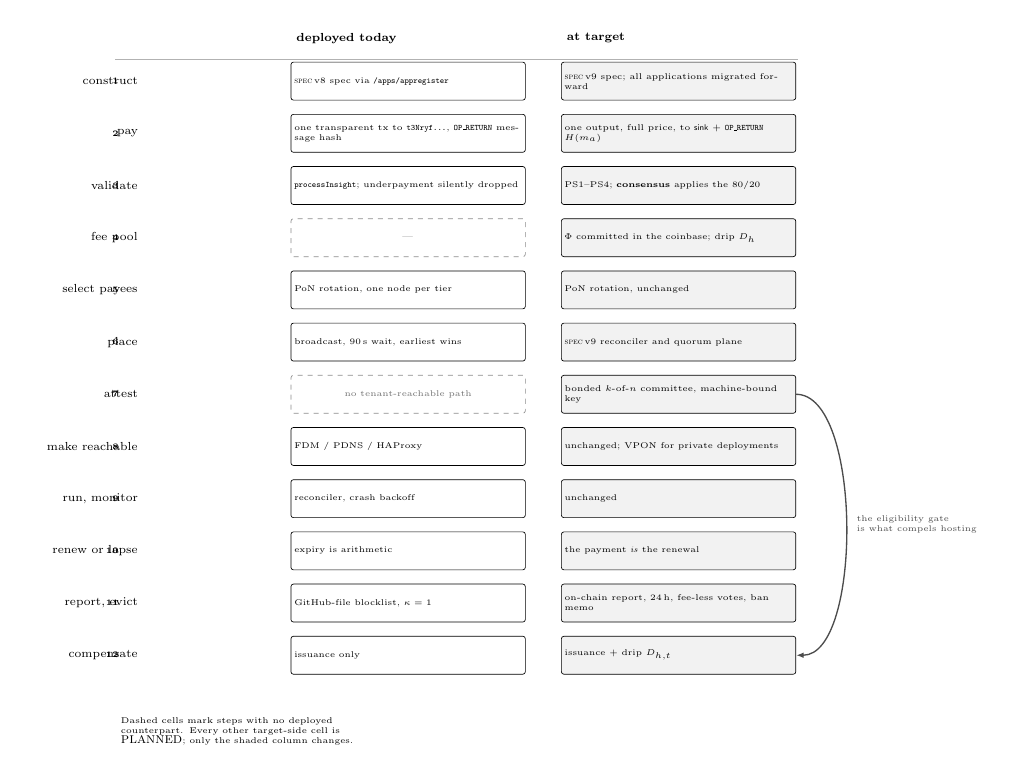
\begin{tikzpicture}[
  font=\tiny, x=1mm, y=1mm,
  cell/.style={draw, rounded corners=1.5pt, text width=48mm, align=left, inner sep=2pt,
               minimum height=8mm, anchor=west},
  tcell/.style={cell, fill=black!5},
  dead/.style={cell, draw=black!45, dashed, text=black!55, align=center},
  stepno/.style={font=\tiny\bfseries, anchor=east},
  stepname/.style={font=\scriptsize, anchor=east, text width=22mm, align=right},
  hdr/.style={font=\scriptsize\bfseries, anchor=west},
]
  \node[hdr] at (5,9)  {deployed today};
  \node[hdr] at (62,9) {at target};
  \draw[black!30] (-32,4.5) -- (112,4.5);

  \node[stepno] at (-30,0) {1};
  \node[stepname] at (-26,0) {construct};
  \node[cell] (d1) at (5,0) {\specv{8} spec via \texttt{/\allowbreak{}apps/\allowbreak{}appregister}};
  \node[tcell] (t1) at (62,0) {\specv{9} spec; all applications migrated forward};
  \node[stepno] at (-30,-11) {2};
  \node[stepname] at (-26,-11) {pay};
  \node[cell] (d2) at (5,-11) {one transparent tx to \texttt{t3Nryf\ldots}, \texttt{OP\_RETURN} message hash};
  \node[tcell] (t2) at (62,-11) {one output, full price, to $\mathsf{sink}$ + \texttt{OP\_RETURN} $H(m_\app)$};
  \node[stepno] at (-30,-22) {3};
  \node[stepname] at (-26,-22) {validate};
  \node[cell] (d3) at (5,-22) {\texttt{processInsight}; underpayment silently dropped};
  \node[tcell] (t3) at (62,-22) {PS1--PS4; \textbf{consensus} applies the 80/20};
  \node[stepno] at (-30,-33) {4};
  \node[stepname] at (-26,-33) {fee pool};
  \node[dead] (d4) at (5,-33) {---};
  \node[tcell] (t4) at (62,-33) {$\pool$ committed in the coinbase; drip $D_\hgt$};
  \node[stepno] at (-30,-44) {5};
  \node[stepname] at (-26,-44) {select payees};
  \node[cell] (d5) at (5,-44) {\PoN{} rotation, one node per tier};
  \node[tcell] (t5) at (62,-44) {\PoN{} rotation, unchanged};
  \node[stepno] at (-30,-55) {6};
  \node[stepname] at (-26,-55) {place};
  \node[cell] (d6) at (5,-55) {broadcast, \SI{90}{\second} wait, earliest wins};
  \node[tcell] (t6) at (62,-55) {\specv{9} reconciler and quorum plane};
  \node[stepno] at (-30,-66) {7};
  \node[stepname] at (-26,-66) {attest};
  \node[dead] (d7) at (5,-66) {no tenant-reachable path};
  \node[tcell] (t7) at (62,-66) {bonded $k$-of-$n$ committee, machine-bound key};
  \node[stepno] at (-30,-77) {8};
  \node[stepname] at (-26,-77) {make reachable};
  \node[cell] (d8) at (5,-77) {\FDM{} / \PDNS{} / HAProxy};
  \node[tcell] (t8) at (62,-77) {unchanged; \VPON{} for private deployments};
  \node[stepno] at (-30,-88) {9};
  \node[stepname] at (-26,-88) {run, monitor};
  \node[cell] (d9) at (5,-88) {reconciler, crash backoff};
  \node[tcell] (t9) at (62,-88) {unchanged};
  \node[stepno] at (-30,-99) {10};
  \node[stepname] at (-26,-99) {renew or lapse};
  \node[cell] (d10) at (5,-99) {expiry is arithmetic};
  \node[tcell] (t10) at (62,-99) {the payment \emph{is} the renewal};
  \node[stepno] at (-30,-110) {11};
  \node[stepname] at (-26,-110) {report, evict};
  \node[cell] (d11) at (5,-110) {GitHub-file blocklist, $\kappa=1$};
  \node[tcell] (t11) at (62,-110) {on-chain report, \SI{24}{\hour}, fee-less votes, ban memo};
  \node[stepno] at (-30,-121) {12};
  \node[stepname] at (-26,-121) {compensate};
  \node[cell] (d12) at (5,-121) {issuance only};
  \node[tcell] (t12) at (62,-121) {issuance $+$ drip $D_{\hgt,t}$};

  % the one cross-track coupling
  \draw[-{Latex[length=1.6mm]}, thick, black!70]
    (t7.east) .. controls +(14mm,0) and +(14mm,0) ..
    node[font=\tiny, right, align=left, pos=0.5, xshift=1mm]
      {the eligibility gate\\is what compels hosting} (t12.east);

  \node[font=\tiny, anchor=west, text width=52mm] at (-32,-137)
    {Dashed cells mark steps with no deployed counterpart. Every other target-side cell is
     \planned; only the shaded column changes.};
\end{tikzpicture}
\caption{The twelve-step application lifecycle, deployed and at target, on a shared step axis. Two steps have no deployed counterpart at all --- there is no fee pool, and no attestation a tenant can reach. The single cross-track edge is \Cref{prop:e2e-gate}: because \PNR{} pays every node regardless of what it hosts, the eligibility gate of step~7 is the only thing that makes step~12 compensate hosting rather than mere presence.}
\label{fig:e2e-twelve-steps}
\end{figure}

% =====================================================================
\subsection{Pass one: the deployed system}
\label{sec:e2e:deployed}

Everything in this subsection is \shipped and is written in the present tense.

\paragraph{1. A tenant constructs a specification.}
The document is a small owner-signed JSON object, and the version it may declare is fixed by chain
height: \specv{8} is enforced from mainnet height \num{1932380}, and above that height a
specification whose top-level keys are anything other than
\texttt{version,\allowbreak{} name,\allowbreak{} description,\allowbreak{} owner,\allowbreak{} compose,\allowbreak{} instances,\allowbreak{} contacts,\allowbreak{} geolocation,\allowbreak{} expire,\allowbreak{} nodes,\allowbreak{}
staticip,\allowbreak{} datacenter,\allowbreak{} enterprise} is rejected outright (\S10)
\srccode{flux/\allowbreak{}ZelBack/\allowbreak{}config/\allowbreak{}default.js}{231--240}
\srccode{flux/\allowbreak{}ZelBack/\allowbreak{}src/\allowbreak{}services/\allowbreak{}appRequirements/\allowbreak{}appValidator.js}{1063--1067}. Seven versions are simultaneously live on the
network --- \specv{2} through \specv{8}, with \num{322} of \num{1195} deployed applications
(\SI{26.9}{\percent}) below \specv{8} --- because the acceptance predicate has a ceiling and no floor
(\S10) \srcmeasured{api.runonflux.io/\allowbreak{}apps/\allowbreak{}globalappsspecifications}{2026-09-03}. The tenant signs the
envelope $\{\texttt{app\allowbreak{}Specification}, \texttt{timestamp}, \texttt{signature}, \texttt{type},
\texttt{version}\}$, where \texttt{type} is \texttt{zelappregister}\slash\texttt{fluxappregister} and the
envelope version --- distinct from the specification version --- is $1$, and \texttt{POST}s it to any
node's \texttt{/\allowbreak{}apps/\allowbreak{}appregister} at \texttt{user} privilege, which is a \texttt{bitcoinMessage}
signature over a login phrase no more than \SI{16}{\hour} old (\S9)
\srccode{flux/\allowbreak{}ZelBack/\allowbreak{}src/\allowbreak{}services/\allowbreak{}appDatabase/\allowbreak{}registryManager.js}{1755--1764}. The receiving node
refuses the request if it holds fewer than $8$ outbound or $4$ inbound peers, refuses a timestamp
more than \SI{1}{\hour} old or more than \SI{5}{\minute} ahead, and refuses a \texttt{version: 9}
specification outright unless \texttt{config.\allowbreak{}fluxapps.\allowbreak{}acceptV9} is set, which defaults to
\texttt{false} with no caller anywhere that sets it (\S9, \S10). It then computes
$\texttt{messageHASH} = \mathrm{SHA\text{-}256}(\texttt{type} \| \texttt{version} \|
\mathrm{JSON}(\texttt{spec}) \| \texttt{timestamp} \| \texttt{signature})$, stores the message with a
\SI{3600}{\second} TTL, broadcasts it, blocks through a fixed confirmation round trip of
$2 \times \SI{1200}{\milli\second}$ plus up to $20 \times \SI{500}{\milli\second}$ of polling, and
returns the hash and nothing else \srccode{flux/\allowbreak{}ZelBack/\allowbreak{}src/\allowbreak{}services/\allowbreak{}appDatabase/\allowbreak{}registryManager.js}{1827--1858}.
The specification carries no \texttt{duration} field and no \texttt{paymentMemo} field; lifetime is
expressed as \texttt{expire} in blocks, and there is no field anywhere in \specv{8} that binds a
payment to a specification other than the hash the tenant is about to put in an
\texttt{OP\_RETURN}.

\paragraph{2. The tenant pays.}
Price is a pure function of the specification and the height, evaluated against a height-scheduled
table with six segments --- genesis plus five revisions --- whose current row takes effect from
height \num{1597156} at $\pricevec = (0.03,\ 0.01,\ 0.004)\flux$ per unit of
$(\mathrm{cpu}, \mathrm{ram}, \mathrm{hdd})$ with surcharges
$(p_{\mathrm{port}}, p_{\mathrm{scope}}, p_{\mathrm{sip}}) = (0.4,\ 0.8,\ 0.4)\flux$ and
$p_{\min} = 0.01\flux$ (\S16) \srcmeasured{api.runonflux.io/\allowbreak{}apps/\allowbreak{}deploymentinformation}{2026-09-03}.
The base is $B(\app,\hgt) = 10\,p_{\mathrm{cpu}}\resvec^{\mathrm{cpu}} +
\tfrac{1}{100}p_{\mathrm{ram}}\resvec^{\mathrm{ram}} + p_{\mathrm{hdd}}\resvec^{\mathrm{hdd}}$ plus
the surcharge terms, quoted per three instances --- $\beta = \lceil B/3 \rceil_2$ per instance,
scaled by the instance count from height \num{1890000} in the three-case form of \Cref{def:price}
--- then scaled by $\dur/L^{\ast}(\hgt)$ with $L^{\ast} = 4\blockslasting = \num{88000}$ blocks at
post-\PoN heights, ceiled to two decimals and only then floored at $p_{\min}$
(\S16) \srccode{flux/\allowbreak{}ZelBack/\allowbreak{}src/\allowbreak{}services/\allowbreak{}utils/\allowbreak{}appUtilities.js}{89--134}
\srccode{flux/\allowbreak{}ZelBack/\allowbreak{}src/\allowbreak{}services/\allowbreak{}appMessaging/\allowbreak{}messageVerifier.js}{736--745}. Duration is bounded to
$\dur \in \{\num{1},\dots,\num{1056000}\}$ blocks --- the floor is height-gated by the validator at
\num{5000}, then \num{100} from height \num{1630040}, then \num{1} from height \num{1964447}, while
the published endpoint still reports \num{5000}
\srccode{flux/\allowbreak{}ZelBack/\allowbreak{}src/\allowbreak{}services/\allowbreak{}appRequirements/\allowbreak{}appValidator.js}{852--862} --- and instance count to
$\ninst \in \{\num{1},\dots,\num{100}\}$ for \specv{8} applications from height \num{2176519}
(\S16). The tenant then broadcasts exactly one transparent transaction paying at least that amount to
the sink address \texttt{t3Nryf\allowbreak{}AQLGe\allowbreak{}Fs9j\allowbreak{}Eoeqsxm\allowbreak{}BN2QLRa\allowbreak{}RKFLUX}, in force from height \num{1670000},
carrying \texttt{messageHASH} in an \texttt{OP\_RETURN} (\S16)
\srccode{flux/\allowbreak{}ZelBack/\allowbreak{}config/\allowbreak{}default.js}{241--245}. All application revenue on the network lands at
that one transparent address, by policy and not by consensus (\S12, \S16).

Both apparent disagreements here are resolved. The duration denominator carries a \PoN{} fork branch --- $22{,}000$ blocks before activation, $88{,}000$ from height $2{,}020{,}000$, the multiplier preserving wall-clock duration --- and \S7's definition now states it. The instance lower bound is $3$ in general and $1$ for \specv{8} applications from height $2{,}176{,}519$; the published endpoint reports $3$ regardless, which is a defect in the endpoint rather than a disagreement between sections \srcdoc{reconciliation record}.

\paragraph{3. The payment is validated.}
No consensus rule sees any of this. Each node's own chain-scan loop,
\texttt{explorerService.\allowbreak{}processInsight}, runs per block, recognises the payment by its output
address, sums \texttt{valueSat} across matching outputs, decodes the temporary-message hash from the
\texttt{OP\_RETURN}, and queues \texttt{messageVerifier.\allowbreak{}checkAndRequestApp} (\S9, \S16)
\srccode{flux/\allowbreak{}ZelBack/\allowbreak{}src/\allowbreak{}services/\allowbreak{}explorerService.js}{309--345,444}. Promotion re-verifies update
signatures against the current permanent owner as an explicit anti-race measure, recomputes the
\PoN-fork-aware expiration height $e_\app$, and admits the specification to \texttt{globalzelapps}
if and only if $v^{\mathrm{obs}} \ge \price \cdot 10^{8}\sat$. If the payment is short, the
registration is \textbf{silently dropped}: a server-side log warning, no error surfaced to the payer,
no retry, and no refund path anywhere in the repository (\S9, \S16)
\srccode{flux/\allowbreak{}ZelBack/\allowbreak{}src/\allowbreak{}services/\allowbreak{}appMessaging/\allowbreak{}messageVerifier.js}{735--763}. The funds are spent
and the deployment does not exist. \S16 records this as the most important correctness gap on the
path this paper otherwise recommends to autonomous software, and states the signed negative
acknowledgement that would repair it as requirement R16.1.

\paragraph{4. Value enters the fee pool.}
\textbf{This step does not exist today.} There is no fee pool. There is no consensus object of any
kind mediating between what a tenant pays and what an operator receives: the payment lands at a
transparent address controlled by policy, and every satoshi any node operator earns is newly issued
(\S7). The step is listed here, empty, so that the two passes stay aligned and so that the reader
sees the gap in the same position in both.

\paragraph{5. Consensus selects the payees.}
Independently of everything above, and with no reference to it, \fluxd awards block production every
\SI{30}{\second}. The \PoN slot is $\tslot(t) = \lfloor (t - t_0)/\spacingpon \rfloor$ with
$\spacingpon = \SI{30}{\second}$, and a confirmed \FluxNode with collateral outpoint $c$ is eligible
for slot $\tslot$ iff $H(c \| h_{\mathrm{prev}} \| \tslot) \le T_\tslot$ --- sortition over the
confirmed-node set, not weighted by collateral amount beyond confirmation (\S4)
\srccode{fluxd/\allowbreak{}src/\allowbreak{}pon/\allowbreak{}pon.cpp}{70--93}. Each block pays one node from each of the three tiers,
selected from a per-tier queue ordered by \texttt{n\allowbreak{}Last\allowbreak{}Paid\allowbreak{}Height} ascending, which is a strict
longest-time-since-paid FIFO (\S4) \srccode{fluxd/\allowbreak{}src/\allowbreak{}fluxnode/\allowbreak{}fluxnode.h}{313--328}. The measured
rotation lengths are $\rot{\tC} = \num{3247}$, $\rot{\tN} = \num{1615}$ and $\rot{\tS} = \num{1627}$
blocks, i.e.\ \SI{27.06}{\hour}, \SI{13.46}{\hour} and \SI{13.56}{\hour}
\srcmeasured{api.runonflux.io/\allowbreak{}daemon/\allowbreak{}listzelnodes}{2026-09-03}. The payee set of the block that
confirms a tenant's payment has nothing to do with that tenant, that payment, or that application.

\paragraph{6. The application is placed across nodes.}
There is no scheduler. Every node runs the same loop against its own gossiped replica of
\texttt{globalzelapps} and reaches its own conclusion (\S9). A node first clears a precondition gate
--- enterprise identity resolved, daemon synced, local database ready, not DoS-flagged, node
confirmed, \fluxbench not erroring, own external IP known, and fewer than
$\texttt{maxAppsPerNode} = 200$ applications installed --- then draws a candidate from the set of
non-expired, under-replicated applications, biased first to those naming its own IP and otherwise
uniformly at random \srccode{flux/\allowbreak{}ZelBack/\allowbreak{}src/\allowbreak{}services/\allowbreak{}appLifecycle/\allowbreak{}appSpawner.js}{78--336}. After
targeting and geolocation filters and a set of soft-deferral branches, it verifies the image against
the Docker Hub whitelist, pulls it, probes port availability through its peers, broadcasts a
\texttt{fluxappinstalling} message carrying its own IP and a self-reported \texttt{broadcastedAt},
and then waits $\texttt{install\allowbreak{}Collision\allowbreak{}Wait\allowbreak{}Ms} = \SI{90}{\second}$
\srccode{flux/\allowbreak{}ZelBack/\allowbreak{}config/\allowbreak{}default.js}{321}. It re-reads the global installing and running lists,
ranks all installing nodes by \texttt{broadcastedAt} ascending, and abandons the attempt if its rank
does not fit the remaining slots. \textbf{Earliest-broadcast-wins is the entire conflict-resolution
mechanism}: no leader election, no quorum, no on-chain arbitration
\srccode{flux/\allowbreak{}ZelBack/\allowbreak{}src/\allowbreak{}services/\allowbreak{}appLifecycle/\allowbreak{}appSpawner.js}{686--703}. Installation proceeds
through \texttt{register\allowbreak{}App\allowbreak{}Locally} into Docker, and from that point every start and stop of the
container goes through one component, the reconciler, described in its own source as the single
level-based actuator, with a crash-backoff ladder of $[0,\ \num{30000},\ \num{300000},\
\num{900000},\ \num{1800000}]\,\si{\milli\second}$ reset after \SI{600000}{\milli\second} of stable
running (\S9) \srccode{flux/\allowbreak{}ZelBack/\allowbreak{}config/\allowbreak{}default.js}{130--131}. Sixty seconds after installing, the
node re-ranks itself by \texttt{runningSince} and uninstalls immediately if it is now surplus.
Convergence is not agreement; it is two opposing correction loops, and both of them correct
over-installation while neither corrects under-installation faster than the next node's random draw
(\S9).

\paragraph{7. The host is attested.}
Nothing a tenant can check. \fluxsas, the attestation service, serves a single listener on
\texttt{127.0.0.1:\allowbreak{}16100} with mutual TLS mandatory and authorisation by client-certificate common
name --- \fluxbench for every route, \texttt{fdm-nginx} for three --- so an external tenant has no
network path to it at all (\S14) \srccode{fluxsas/\allowbreak{}src/\allowbreak{}api\_server.h}{1042--1053,220--252}. Even with
a path, the signature would not say what a tenant needs: the Ed25519 key used by \texttt{/v2/attest}
for the default, \texttt{cdn}, \texttt{mesh} and \texttt{app} purposes is derived from static values
compiled identically into every \fluxsas binary, so a valid attestation demonstrates possession of
something every copy of the software contains rather than that a particular machine booted a
particular image (\S14) \srcprivate{\SAS{} API server}. One layer down, the eligibility
gate that admits a node to the paid set at all is a benchmark signature produced by a process on the
operator's own host and verified against \texttt{vec\allowbreak{}Benchmarking\allowbreak{}Public\allowbreak{}Keys}, five network-wide keys
with timestamp validity windows --- collateral binds the tier, and the benchmark signature does not
bind the hardware to it (\S4) \srccode{fluxd/\allowbreak{}src/\allowbreak{}chainparams.cpp}{233--240}. What \emph{does} do real
work is the boot chain: a Flux-controlled Secure Boot Platform Key pinned by hash inside \texttt{fes},
fail-closed exit codes \num{50}--\num{57} that power the machine off rather than continue, a TPM2
seal against PCR~7, and a dm-verity root filesystem (\S14). But the allow-list of known-good verity
root hashes is served by two Flux-operated web endpoints that \textbf{fail open} --- if both are
unreachable, the watchdog treats the node as secure and does nothing
\srcprivate{\SAS{} watchdog}. The honest summary of this step is that measured boot
imposes real cost on a remote attacker, and that the assurance a node offers is a Flux-operated one
rather than a hardware-rooted, tenant-verifiable one.

\paragraph{8. \FDM and \PDNS make the application reachable.}
The reverse path from a hostname to a container is Foundation-operated end to end (\S12). \FDM does
not talk to \fluxd or to any peer-to-peer layer: it polls one Foundation-operated REST API,
\texttt{api.\allowbreak{}runonflux.\allowbreak{}io}, for \texttt{apps/\allowbreak{}globalappsspecifications} every \SI{30}{\second} under an
\texttt{ETag}, \texttt{apps/locations} every \SI{10}{\second} unconditionally, and permanent messages
every \SI{120}{\second}, and no fallback source exists anywhere in the codebase
\srccode{flux-domain-manager/\allowbreak{}src/\allowbreak{}services/\allowbreak{}flux/\allowbreak{}dataFetcher.js}{47--91}. Names are computed by string
concatenation --- \texttt{$\app$\_$P$.app2.runonflux.io} per port and \texttt{$\app$.app2.runonflux.io}
as the main alias --- and served either by Cloudflare in strict DNS-only mode or by the self-hosted
\PDNS zone service. The \FDM host's own HAProxy terminates TLS against every \texttt{.pem} under
\texttt{/\allowbreak{}etc/\allowbreak{}ssl/\allowbreak{}fluxapps/\allowbreak{}} and routes on the \texttt{Host} header to one of the application's
container IPs, with per-server health checks of \texttt{inter 3s fall 2 rise 2 fastinter 500},
i.e.\ an approximately \SI{6}{\second} detection floor
\srccode{flux-domain-manager/\allowbreak{}src/\allowbreak{}services/\allowbreak{}haproxyTemplate.js}{260--319}. Sixteen Foundation-run
\FDM/CDM hosts serve this path for the whole network; roughly two dozen game-server application types
bypass HAProxy entirely through a single, unreplicated \texttt{flux-\allowbreak{}apps-\allowbreak{}dns-\allowbreak{}manager} instance
(\S12). Inside the fleet, container-to-container names resolve through \fluxdnsd, which despite the
name is a purely local file-tail resolver over a \texttt{membership.\allowbreak{}json} that \FluxOS writes, with a
fixed \SI{5}{\second} answer TTL and \texttt{REFUSED} rather than \texttt{SERVFAIL} when it holds no
snapshot (\S12).

\paragraph{9. It runs and is monitored.}
The reconciler holds the container to its desired state, resolved from four inputs in strict priority
order with the operator's own lock winning over all (\S9). Around it run the periodic monitors: a
node-status monitor every \SI{1.5}{\minute}, an application-availability check every
\SI{3}{\minute}, a CPU-usage check every \SI{900000}{\milli\second}, an image-compliance sweep every
\SI{3600000}{\milli\second}, and a storage check every \SI{20}{\minute} (\S9)
\srccode{flux/\allowbreak{}ZelBack/\allowbreak{}src/\allowbreak{}services/\allowbreak{}serviceManager.js}{433--563}. Location records carry a
\SI{7500}{\second} TTL, and a departing node's \texttt{fluxnodesigterm} broadcast extends its
applications' location TTL by $\texttt{SIGTERM\_EXPIRY\_MS} = \SI{420000}{\milli\second}$ rather than
expiring them at once. Where the operator has opted an application in, \texttt{flux-\allowbreak{}telemetryd} ships
per-container telemetry to a customer-chosen backend every \SI{15}{\second}. Crucially, none of this
is metering: \Flux prices reservation, not consumption, so there is no usage counter to read, to
attest, or to dispute (\S16). The only disputable fact is the binary one --- did the application run
--- and that is observable by third parties from location records, \FDM health checks, and the
tenant's own probes.

\paragraph{10. It renews or lapses.}
Expiry is arithmetic, not a decision. Entitlement is the predicate
$\mathrm{Ent}(\app,\hgt) = \indic{\hgt \le e_\app}$, where $e_\app$ was fixed at promotion from
$(\hgt_0, \dur)$ and is a function of the confirmed chain prefix alone (\S16). Every node evaluates
it independently and reaches the same answer, and a periodic pass every
$\texttt{expire\allowbreak{}Flux\allowbreak{}Apps\allowbreak{}Period} = 100$ blocks removes what has passed
\srccode{flux/\allowbreak{}ZelBack/\allowbreak{}config/\allowbreak{}default.js}{298}. A renewal is an update, priced at
$\max\{p_{\min},\ 0.9\,(\price - \varpi\price_{\mathrm{prev}})\}$ where $\varpi$ is the unused fraction
of the previous term (\S16). \textbf{There is no grace window, no suspension state, and no
data-retention guarantee}: when the paid-through height arrives the entitlement stops, and the
removal path is the ordinary one. That is a consequence of the design rather than an omission ---
Property ``No standing obligation'' in \S16 shows that any grace state would have to be a function of
information not in the chain prefix --- but it is a real difference from what a tenant used to
hyperscaler billing expects. The only automatic renewal that exists is
\texttt{appsmonitor}, a Foundation-operated daemon that renews applications whose owner keys the
Foundation itself holds, alongside a hardcoded single-address \texttt{usersToExtend} allow-list
permitted to submit expire-only extensions on any owner's behalf (\S16).

\paragraph{11. It may be reported and evicted.}
There is no quorum. Moderation is a publisher: \FluxOS fetches
\texttt{helpers/\allowbreak{}blockedrepositories.\allowbreak{}json} from \texttt{raw.\allowbreak{}githubusercontent.\allowbreak{}com/\allowbreak{}RunOnFlux/\allowbreak{}flux},
caches it, and every \SI{1}{\hour} removes every locally installed application whose image, owner
address or specification hash matches, spacing removals \SI{3}{\minute} apart (\S9, \S23)
\srccode{flux/\allowbreak{}ZelBack/\allowbreak{}src/\allowbreak{}services/\allowbreak{}appSecurity/\allowbreak{}imageManager.js}{179--195,644--676}. The wider
\texttt{fluxos-\allowbreak{}network-\allowbreak{}policy} channel carries the same shape for blocked and vetted repositories,
the enterprise-node owner map, a node-tampering blocklist and a $\sim$2.0-million-row geolocation
table, fetched every \SI{6}{\hour} or \SI{12}{\hour} and enforced fleet-wide with no canary and no
staged rollout (\S12). The documents are unsigned; by the component's own account their authenticity
rests on GitHub and on who can merge, and branch protection deliberately imposes no second-reviewer
requirement. \S23 states the resulting measure exactly: the number of parties whose agreement removes
an arbitrary application from every node is $\kappa_{\mathrm{deployed}} = 1$, the authentication on
the decision is nothing, the record a node can verify is nothing, and the latency to fleet-wide
effect is bounded by \SI{7}{\hour} (\SI{13}{\hour} for the tampering list).

\paragraph{12. Operators are compensated.}
From issuance alone. For $\hgt \ge \hpon = \num{2020000}$ the block subsidy is
$\subsidypon(\hgt) = s_{r(\hgt)}$ with $s_0 = 14\flux$, $s_{k+1} = \lfloor s_k \cdot 9/10 \rfloor$,
and $r(\hgt) = \min(\lfloor (\hgt - \hpon)/\redint \rfloor,\ \redmax)$ for
$\redint = \num{1051200}$ blocks and $\redmax = 20$ (\S5)
\srccode{fluxd/\allowbreak{}src/\allowbreak{}main.cpp}{2799--2816}. Of that, the three tier payees receive
$\lfloor \subsidypon(\hgt)\,\tbase{X}/14\flux \rfloor$ with
$(\tbase{\tC},\tbase{\tN},\tbase{\tS}) = (1,\ 3.5,\ 9)\flux$, and the remainder
$\devfund(\hgt) = 0.5\flux$ at $r = 0$ --- $1/28$, or \SI{3.57}{\percent}, of \PoN emission --- is a
consensus-enforced payment to the hardcoded address \texttt{t3h\allowbreak{}Pu1YDe\allowbreak{}GUCp8m7BQCnn\allowbreak{}NUm\allowbreak{}RMJBa5Rady\allowbreak{}A}
(\S5) \srccode{fluxd/\allowbreak{}src/\allowbreak{}main.cpp}{2877--2895}. Emission does not stop: after twenty reductions the
subsidy freezes at $\num{1.70207313}\flux$ per block, i.e.\ $\num{1789219.274256}\flux$ per year,
indefinitely (\S5). \textbf{Nothing the tenant paid in step~2 reaches any of these payees.} The
tenant's money is at one address and the operator's money is newly minted, and the only thing
connecting them is that both happen on the same chain.

% =====================================================================
\subsection{Pass two: the target architecture}
\label{sec:e2e:target}

Everything in this subsection is \planned. Nothing in it is deployed, no part of it is scheduled to a
height except where a height is explicitly named as proposed, and no sentence below should be read as
a statement about the network as it runs. Where the target depends on something unbuilt or undecided
that dependency is named at the step, in the same paragraph.

\paragraph{1. A tenant would construct a specification.}
The document would be a \specv{9} specification carrying \texttt{duration} as a first-class field, a
\texttt{paymentMemo} of up to \num{512} characters in the draft schema, a \texttt{referralCode}, and
a \texttt{machineType} drawn from $\{\texttt{standard}, \texttt{gpu}, \texttt{vps}\}$, with the four
\specv{8} renames applied and \texttt{enterprise} removed (\S10). Applications already deployed would
not be left behind on older versions and would not be offered the choice: the settled migration is
\textbf{forced}, an application-update message carrying a special signature that rewrites every
application forward onto \specv{9}, after which updates on older specification versions would be
disabled and, once the fleet had moved, the legacy validation paths removed (\S10)
\srcintent{design intake}. That supersedes the version-floor-plus-deprecation
design and is the better answer to the \num{322}-application, \SI{26.9}{\percent} legacy tail of
step~1 of the first pass, because it would clear the tail at one moment rather than letting it trail
off at each owner's own pace. It also creates a capability this paper names rather than lets a reader
find: a key able to rewrite a tenant's signed specification without that tenant's signature, which
\S10 places in the same class as the unsigned network policy, the release channel and the
emergency-block keys, and which the team's decision bounds as single-use, migration-scoped and
hardcoded --- with no opt-out for an owner who would rather remain on the document they signed
(\S10, C40).

Five things are undecided or unbuilt at this step and each is load-bearing. \specv{9} has no
enforcement height in shipped configuration or on the live pricing endpoint --- the height itself is
now settled at $\hstar = \num{3050000}$ (\S10) but is not yet shipped --- and \S10 states the
ordering constraint that the height must \emph{follow} implementation of the three economic fields
rather than precede it. \texttt{paymentMemo}, \texttt{referralCode} and \texttt{machineType} have
\textbf{zero consumer code anywhere in \FluxOS} (\S10) --- they are exactly the fields \PNR,
referrals and the VPS tier are each stated to depend on. The RFC-0 draft has no signature field at
all and states its canonicalization rules as prose \texttt{MUST}s with no schema or code enforcement,
which for a document meant to be compared byte-for-byte across roughly \num{6500} independent
validators is the defect to name (\S10). The removal of \texttt{enterprise} arrives with no declared
replacement, so \specv{9} as drafted cannot express a private deployment at all, against
\SI{18.7}{\percent} of currently deployed applications that use it (\S10). And the migration key's
scope --- whether \fluxd itself would reject a forced update touching anything beyond the version
field and the four renames, or whether that restraint would live only in the tooling that constructs
the message --- is open in \S10, as is whether the key is retired when the migration completes rather
than left live in a binary. Where the submitter is autonomous software rather than a person, the
specification would travel with a delegation certificate
$\mathsf{cert} = (pk_\agent, \scopeset, \budget, [t_0,t_1], \mathsf{rev}, \nu)$ signed by the
principal's full 2-of-2 ceremony, and a node would accept it by a predicate computable from the
message, its own chain state at $\hgt$, and nothing else (\S17). The deployment half of that
authority composes with machinery that already runs; the spending half does not, and \S17 classes it
as not achievable on the \Flux L1 without either a new trusted party or new consensus state.

\paragraph{2. The tenant would pay.}
One transaction, one recipient, one memo. The settled shape is a single transparent output paying the
full price $\price(\app,\hgt)$ to $\mathsf{sink}$ --- one application-payment address carried as a
consensus constant from $\hpa$ onward --- together with one zero-value \texttt{OP\_RETURN} whose data
field is the \num{32}-byte $H(m_\app)$; these are rules PS1 and PS2 of \S7
\srcintent{design intake} \srcdoc{reconciliation record}. There would be no
second output, no fee component and no new transaction type. The payer would construct one recipient
and its own change and would perform no other arithmetic, so any wallet able to pay an address and
attach a memo --- and any agent holding a bare wallet API --- could construct a valid payment without
linking a \Flux-specific library or waiting for tooling to be rolled out. \S7 records the deployed
\CumulusVPN entitlement path as the existence proof for exactly that shape, and records the two
shapes not taken and why: a fee-carried share would make the amount a function of the sending
wallet's change calculation, and a typed transaction would put a library dependency in front of every
payer. Direct per-deployment settlement would remain the default and the recommended path for
autonomous software, for the reason \S16 proves: entitlement is a function of the confirmed chain
prefix alone, so no account, no stored credential and no relationship outliving the deployment would
be involved. The alternative would be the custodial path \S16 documents as \shipped, in which a
facilitator holds the user's keys and pays the chain for them, and over which \S16 recommended that a
recurring charge be authorised by a \S17 certificate whose scope $\scopeset$ is restricted to
\emph{renew this application at no more than this price} under budget $\budget$, because that is the
only one of the three candidate authorities that removes the custodian rather than relocating it ---
a recommendation the settlement has since overtaken, since the protocol is to offer no automatic
renewal at all and recurrence stays in the service layer, by custody (\Cref{rem:no-protocol-renewal}).
Two of this step's open decisions were closed by the settlement: O3, the
memo's semantics, is $H(m_\app)$ in an \texttt{OP\_RETURN}, and O18, the serialisation and the
enforcement boundary, is the single-output shape with the split applied by consensus. Two remain.
O14, the identity of $\mathsf{sink}$, is unfixed --- keeping the address in use today preserves
tooling and one continuous history but mixes pre-$\hpa$ spendable receipts into the counter of
step~4, and a consensus-level address is a consensus-level commitment. O8, which payment channels
must settle through $\mathsf{sink}$ at all, is the load-bearing one, because every channel outside it
is revenue the consensus split never touches. Where a deposited balance would live --- on-chain,
\FluxOS-held or wallet-held --- was the architectural choice \S16 could not make, alongside the
authorisation object; both are now settled out of protocol scope, the balance held off-chain by a
third-party operator and no authorisation object existing at the protocol level at all
(\Cref{rem:balance-location}, \Cref{rem:no-protocol-renewal}).

\paragraph{3. The payment would be validated.}
Two consensus rules would run at $\hgt \ge \hpa$, and neither would involve the payer. PS3 makes any
output paying $\mathsf{sink}$ unspendable, so a block containing such a spend would be invalid and
the value would leave circulation at the moment of payment. PS4 divides what arrived:
$A_\Phi = \lfloor r(\hgt)\,v/100 \rfloor$ with $r(\hgt) = 100\,\nodeshare(\hgt) \in \mathbb{Z}$ is
credited to the fee pool, and $A_F = v - A_\Phi$ is credited to the Foundation, the single floor
taken once per received output and favouring the Foundation by strictly less than $1\sat$ (\S7).
\FluxOS would check three things and no others: that a payment exists, that it carries $H(m_\app)$,
and that it covers $\price(\app,\hgt)$. \textbf{The payer splits nothing and can therefore get
nothing wrong, and \FluxOS has no split to police.} That is the point \S7 makes about the decision
rather than about the outcome: choosing the single-output shape for \emph{wallet compatibility} also
removed the \emph{enforcement} ambiguity, and both properties came from one choice (C38). Three
consequences follow and \S7 proves them together. A wallet could not mis-round or omit a share that
it never computes. A \FluxOS release could not alter $\nodeshare(\hgt)$, the tier partition or the
destination of either share, because those would be evaluated in \texttt{ConnectBlock} rather than in
\FluxOS, and a node running a changed rule would be rejected by every other node. And the coinbase
would gain no output, because both shares would be added to outputs that already exist. What consensus
would \emph{not} fix is the amount: \FluxOS would still compute $\price$ from the height-scheduled
table, and \S7's formulation is the honest one --- \emph{consensus would fix the distribution, policy
would fix the base}, against a table revised five times with the CPU rate falling \num{100}-fold.
O7 --- whether received value can be visible to consensus while the payer is shielded --- is moot:
both shielded pools are to be retired (\S\ref{sec:shielded-retirement}), so all settlement is
transparent. Whether the table's rebasing becomes rule-based or oracle-driven is O9, settled as rule-based in
\S\ref{sec:pnr:recommended}, which leaves what the rule is open.
The signed negative acknowledgement of requirement R16.1, which would make an underpaid registration
observable to its payer, is specified in \S16 and is not built --- and it is the one repair this step
still owes an autonomous payer.

\paragraph{4. Value would enter the fee pool.}
This is the step with no deployed counterpart, and it is the mechanism the whole target economy rests
on. The fee pool would be a single consensus-state integer $\pool_\hgt \in \mathbb{Z}_{\ge 0}$ in
$\sat$ with $\pool_{\hpa-1} = 0$, \emph{committed in the coinbase} of every block from $\hpa$ and
recomputed by every validator from the parent value and the block body as
\[
  \pool_\hgt \;=\; \pool_{\hgt-1} \;-\; D_\hgt \;+\; \text{receipts}_\hgt ,
\]
with a block whose committed value differs from the recomputation being invalid (\S7, rule PC)
\srcintent{design intake} \srcdoc{reconciliation record}. That closes O2, and
the reasons \S7 gives for it are the ones that matter to a reimplementer rather than to a reader:
reorg-exactness would come free, because the pool would be a pure function of the chain, so a reorg
would recompute it with no rollback journal and no way for the pool to diverge from the UTXO set; no
new database would be introduced, because the coinbase parsing and enforcement path the commitment
needs is the one \fluxd runs every block for the dev-fund minimum and the three tier payouts
\shipped; and a divergent implementation would be rejected at the block where it first arises rather
than one block later. \S7 rejects a separate store on this network's own
precedent --- the \FluxNode registry needed a crash-recovery marker and a repair RPC precisely
because a side database can diverge from the coins database --- and rejects a header field as the
widest-blast-radius fork available.

Nothing would be added to the coinbase at any point in the mechanism. The Foundation's
\SI{80}{\percent} would flow through the \emph{existing} dev-fund output, the operator drip would be
added to the \emph{existing} three tier outputs, and the pool commitment itself would occupy the
coinbase's data-bearing field rather than a value-bearing one (\S7, I4). Supply would be conserved by
construction and not by bookkeeping: PS3 removes what is paid to $\mathsf{sink}$ from circulation and
the coinbase re-issues it, so circulating supply would differ from \S5's issuance schedule by exactly
the pool balance in flight, $\supply'(\hgt) = \supply(\hgt) - \pool_\hgt$, which at steady state is
\SI{30}{\day} of the operator share. The same rule turns the sink's balance into a
\emph{public cumulative-revenue counter}: the gross application revenue settled through this path
since $\hpa$ would be the balance of one address, queryable by anyone, publishable by no party in
particular and withholdable by none --- which is what would let \S\ref{sec:evaluation} replace an assumed $100\flux$
per application per month with a measurement, and what would make O17 closable by observation rather
than by disclosure. One qualification travels with the counter and must not be dropped: it would
measure only what settles through this path, so every channel left outside it by O8 is revenue the
counter would not see and the split would not touch.

Four things about the pool were undecided, all four are now settled (three at
\Cref{tab:pnr-recommended}, O21 at \Cref{rem:pnr:o21}), and two hard security requirements stand
regardless. O11, whether the pool is seeded at activation,
decided whether the mechanism ramps over roughly ninety days or switches on --- it is settled at no
seed, because a seed would be a one-off Foundation transfer to operators and would have to be
labelled one. O5 and O6, the destinations of a tier share with no payee and of the $\le 2\sat$
partition residue, are worth almost nothing per block and are nonetheless fixed explicitly --- both
stay in $\pool$ --- because an implementation difference in either is a chain split. O21, created by
the settlement itself, is settled on the same-block option (\Cref{rem:pnr:o21}): the division is
applied on arrival, at the $\nodeshare$ in force at the receipt height, and the Foundation share is
paid through the dev-fund output of the block that receives it, which needs no second accumulator
and imposes no lag but makes that output depend on the block body rather than on the parent state
alone --- a property the one-block deferral would have restored, and which is given up because it
serves a verifier \S\ref{sec:bridge} establishes cannot exist for \Flux. The requirements are S1 and
S2. An emergency block, produced through the hardcoded 2-of-4 key path with no time or stall gating,
must not drip, or the holders of two of four keys could accelerate the release of accumulated fees
--- $\pool_{\hgt-1}/\drip$ per block, paid to whichever nodes head the queue, including any they
operate --- on every block they produce; they could not redirect it, because an emergency block
still fills the deterministic tier payout (\S7). And forfeitures from the moderation mechanism of
step~11 must never enter $\pool$ (\S7).

\paragraph{5. Consensus would select the payees, and the pool would drip to them.}
The rotation would be unchanged: \PNR would consume \PoN's payee set and add no selection mechanism
of its own (\S7). Each block would drip $D_\hgt = \lfloor \pool_{\hgt-1}/\drip \rfloor$ from the
\emph{parent} state, partitioned by tier as
$D_{\hgt,t} = \lfloor 2\tbase{t}D_\hgt/27 \rfloor$ over the integers $2\tbase{t} \in \{2,7,18\}$,
giving $(\tierratio{\tC}, \tierratio{\tN}, \tierratio{\tS}) = (2/27,\ 7/27,\ 18/27) =
(\SI{7.41}{\percent},\ \SI{25.93}{\percent},\ \SI{66.67}{\percent})$, and the existing tier output
would carry $\subsidy_t(\hgt) + D_{\hgt,t}$ rather than a new output. The pool would update as
$\pool_\hgt = \pool_{\hgt-1} - D_\hgt + \epsilon_\hgt + U_\hgt + F_\hgt$. Two properties follow and
both matter for how a reader should read this step. At steady state the drip equals the inflow, so
the pool is a delay line with time constant $\drip$ blocks and not a treasury that anyone could
choose how to spend (\S7). And because the drip is taken from the parent state and is linear in it,
an operator who is also a tenant and times a payment to land the block before its own node is paid
recaptures exactly $\tierratio{t}/\drip$ of its contribution --- $7.72 \times 10^{-6}$ for a Stratus
node at the settled $\drip$, three orders of magnitude inside the design's own requirement (\S7). The
drip constant is settled at $\drip = \num{86400}$ blocks, exactly \SI{30}{\day} at \SI{30}{\second}
spacing, which closes O1 \srcintent{design intake}. The trade-off it resolves
does not disappear with the decision, and \S7 restates it so that a later revision starts from it:
within-tier spread $\approx \rot{\tC}/\drip$ and targeted recapture $\approx \tierratio{t}/\drip$
both fall with $\drip$, while lag, activation ramp and steady-state pool size $F\drip$ all rise with
it, over the domain $[10^{4},\ 2\times10^{5}]$ blocks in which the constant was chosen. Because
$\drip$ would be a consensus constant, revisiting it would be a network upgrade rather than a
configuration change --- so what accompanies the value is O12, settled as a documented review
trigger at $2\times$ the current Cumulus count rather than an automatic rule, since at $4\times$ the
decay-side spread reaches \SI{16}{\percent}.

\paragraph{6. The application would be placed across nodes.}
Placement would run under the \specv{9} reconciler: roughly \num{25} focused service packages
including \texttt{appLifecycle}, \texttt{appMesh} and \texttt{appPlacement}, a drain server exposing
\texttt{drain\_app}\slash\texttt{stop\_app} over a UNIX-socket JSON-RPC endpoint, and per-application-CA
backend TLS under which a node generates a local Ed25519 keypair and obtains a \SI{30}{\day} host
certificate signed by the application's own certificate authority through \fluxbench, renewed
automatically (\S10). That substrate is built and tested --- \num{289} unit-test files with
\num{7763} test cases run on every push --- and it lives on an individual contributor's fork rather
than in the organisation repository, which \S10 and \S23 both record as a fact about where
development authority sits (\S10). Two things are inert. \texttt{quorum\allowbreak{}Grant\allowbreak{}Activation\allowbreak{}Height}, the
height gate for the fork's mastership and active-standby quorum plane, is read by production code but
set only in integration-test fixtures and is absent from shipped configuration (\S10). And the
conflict-resolution rule itself would be unchanged: nothing in any drafted section replaces
earliest-broadcast-wins, so the target inherits both the \SI{90}{\second} wait and the honesty
assumption on \texttt{broadcastedAt} that \S9 states.

\proposednote{Earliest-broadcast-wins is retained at target. No section of this paper specifies a
replacement, and on reflection none is needed for the reason \Cref{rem:pnr:framing} gives: because
\PNR{} pays no marginal reward for hosting, winning a placement race carries no direct income, so the
race has no financial stakes and the incentive to game it is weak. A deterministic scheduler would be
preferable on other grounds --- predictability, capacity balancing --- but it is a \FluxOS{} design
question, not a consensus one, and replacing a mechanism that is not currently being gamed is not a
prerequisite for anything else in this paper. \srcinferred.}

\paragraph{7. The host would be attested.}
The proposed answer is not a better key but a design that stops depending on a key and depends on
collateral instead (\S14). A node would opt into the attested tier by posting a bond $\beta_i$
\emph{separate from} its \FluxNode collateral, which would remain self-custodied and untouched by any
slashing path. A claim would be a tuple
$\mathsf{cl} = (\mathsf{subject}, \mathsf{predicate}, \mathsf{value}, \hgt, \mathsf{nonce})$ signed under
the node's key; a committee of $n$ bonded nodes would be sampled deterministically as
$\mathcal{C}(\mathsf{cl}) = \mathrm{Top}_n(i \mapsto H(\mathsf{subject} \| \mathsf{prevHash}(\hgt) \| i))$,
reusing the sortition \fluxd already implements for \PoN slot eligibility; a claim would be accepted
at $k$ of $n$ identical signatures, challengeable for a window $\Delta_{\mathrm{chal}}$ by any party
posting $\beta_{\mathrm{chal}}$, and a resolved challenge would slash each original signer by a
fraction $s$ (\S14). Requirement~0 gates the entire construction: the attestation signing key would
have to be derived from or sealed to a per-machine hardware root, which
Property~``Attestation is not machine-bound'' in \S14 says it is not, and a tenant-reachable
verification path would have to exist where today there is none. Absent the first condition a bond
would secure a signature anyone holding the software can produce, making it forfeitable for
statements the bonded party never made. The four committee parameters are recommended by \S14 at
$n = 9$, $k = 6$, $\Delta_{\mathrm{chal}} = \num{2880}$ blocks and $s = 1$, and the bond-sizing
function at a floor $\beta_{\min}$ or a fixed fraction of the value secured, whichever is larger,
with both coefficients still to calibrate: $\beta_i$ must scale with the value secured by the claims
a node is sampled to sign, not with its \FluxNode tier, because a fixed bond cannot secure an
unbounded reserve (\S14). Admissible claim classes are likewise recommended as the objectively
re-checkable class only at launch, \S14 explicitly declining to invent a resolution procedure for
general computation-integrity claims.

\paragraph{8. \FDM and \PDNS would make the application reachable.}
This is the step where the target is least specified, and the paper should not pretend otherwise. The
requirement is legible from \S12's centralization inventory: \texttt{api.\allowbreak{}runonflux.\allowbreak{}io} is the sole
application-discovery source with no on-chain or peer-to-peer fallback coded anywhere, so any
decentralization of reachability starts with a discovery fallback that does not exist. Two further
interfaces would be needed and neither is designed. First, \S23 records as open whether \FDM and
\PDNS honour a ban by dropping routes at $\hgt_b + \Delta_{\mathrm{exec}}$, where $\hgt_b$ is the
height of the coinbase carrying the ban memo of step~11 --- without which a banned application would
remain reachable at its name until the last node had removed it, and with which the
Foundation-operated reachability plane acquires a new dependency on moderation state. Second, private overlay deployments (\VPON s) are a roadmap item with no wire
protocol, key-management scheme or placement-isolation mechanism specified anywhere; \S12 states the
two requirements a \VPON would have to meet --- membership gated by possession of a private key
rather than by resolvability, and a reachability plane not positioned to learn which nodes host a
private deployment or on whose behalf --- and states that the construction is open. The shipped
\CumulusVPN transports (AmneziaWG obfuscation, WireGuard-over-TLS, client-side multi-hop) are cited
by \S12 as building blocks a future design would not have to invent, not as a design.

\paragraph{9. It would run and be monitored.}
The target changes less here than anywhere else, and deliberately. Reservation pricing would remain,
so there would still be no metering on the application path, no counter to attest and no counter to
dispute; \S16 notes that this is the same choice \S7 makes one layer down when it removes any
metering or attestation dependency between payment and placement. What \specv{9} would add is
drain-aware shutdown: marking a component draining would trigger an immediate presence rebroadcast,
so the signal a routing layer consumes rides the gossip path \FluxOS already uses (\S10). The
companion \texttt{flux-shutdownd} pipeline is \inprogress --- its signal-and-cleanup stages are wired
to production events, while drain-broadcast and \texttt{preStop} execution are modelled and
unit-tested but not yet reachable (\S9). Whether the target architecture should acquire an
availability remedy at all is settled by \S16 as no, at the protocol layer (\Cref{rem:no-sla}): the
minimum viable input would be a third-party-observable availability record, which does not exist, and the
cost would be reintroducing the metering dependency the design removed.

\paragraph{10. It would renew or lapse.}
Two paths, and conflating them is the error this step exists to prevent. On the default path there
would be nothing to renew, because \textbf{the payment is the renewal}: a tenant wanting another term
would send another payment of the shape of step~2, and entitlement would remain what \S16 proves it
to be --- a function of the confirmed chain prefix alone. There would be no standing obligation, no
balance to track, no charge to authorise, and \emph{no lifecycle state machine at all}, so there
would be nothing for a policy to decide and no state a policy could get wrong. That is a consequence
of the design and not a gap in it: \S16's corollary is that a grace or suspension state would have to
be a function of information absent from the chain prefix, so the direct path cannot carry one
without surrendering the property that makes it the recommended path for autonomous software. Expiry
would stay arithmetic.

The second path would remain custodial, and \S16 documents what it is as \shipped rather than
projecting what it might become: a \emph{prepay-and-forward facilitator} that holds both of a user's
private keys --- the identity key whose address is written into the specification's \texttt{owner}
field, and the payment key --- charges a card, and pays the chain on the user's behalf, keeping no
user balance and no withdrawal path (C42). The four-state machine
$\mathrm{st}(\app,\hgt) \in \{\textsf{funded}, \textsf{grace}, \textsf{suspended}, \textsf{evicted}\}$
belongs to something else: a deposited-balance credits layer that \S16 specifies in full and marks
explicitly as unimplemented. Were it built, a renewal would fire at
$\hgt = e_\app - \Delta_{\mathrm{pre}}$ if the balance covers $\price^{\mathrm{ren}}$; a lapse would
move the application to \textsf{grace}, where it would keep running and keep its data; after
$G_{\mathrm{g}}$ blocks it would move to \textsf{suspended}, containers stopped but not removed and
volumes retained; and only after a further $G_{\mathrm{s}}$ blocks would it be \textsf{evicted} and
its data destroyed. The separation of stopping from deleting is that layer's design commitment and it
has a price \S16 bounds exactly: revenue forgone over the whole window is at most
$\ninst_\app\,p_{\mathrm{hdd}}(\hgt)\,\resvec^{\mathrm{hdd}}(\app)\,(G_{\mathrm{s}} +
G_{\mathrm{g}})/L^{\ast}(\hgt)$, linear in the declared disk footprint and independent of the CPU and
RAM reservation. Its four parameters are settled at \Cref{tab:credit-params} --- $G_{\mathrm{g}} =
\num{2880}$ blocks from the domain $[240, 2880]$, $G_{\mathrm{s}} = \num{20160}$ from
$[2880, 43200]$, $\Delta_{\mathrm{pre}} = \num{120}$ from $[20,\infty)$, bounded below by
confirmation depth plus propagation, and the resumption charge $\price^{\mathrm{res}}$ at one renewal
period from $[0,\infty)\flux$ --- and all four are service-layer values, because the two
architectural choices they were downstream of are settled out of protocol scope: a deposited balance
lives off-chain with a third-party operator, and nothing in the protocol authorises a recurring
charge (\Cref{rem:balance-location}, \Cref{rem:no-protocol-renewal}). One requirement crosses from
\S7 and constrains any answer: after $\hpa$ every
application-hosting charge, whatever the payment channel, must settle as exactly one L1 payment to
$\mathsf{sink}$, or the consensus split is void and the revenue counter of step~4 under-reports ---
which is why a credit balance may not become an off-chain ledger of hosting charges. And whichever
path a tenant took, the invariant that makes the custodial one optional rather than structural would
hold: for every deployment reachable through a custodian or through credits, the same deployment is
reachable at the same height through an explicit transaction the tenant signs and broadcasts itself
(\S16).

\paragraph{11. It could be reported and evicted.}
Every step of the decision would be a chain fact, and that is the whole difference from step~11 of
the first pass. A report would be a \fluxd transaction of a new \FluxNode-family type carrying the
application hash to be banned, shaped after the deployed start and confirm transactions and
\emph{indexed}, so that any node could enumerate the open reports on an application from its own
chain state; it would carry no fee and no bond, and its confirmation height $\hgt_0$ would fix the
canonical clock and \emph{freeze the electorate} (\S23)
\srcintent{design intake}. A window of
$\Delta_{\mathrm{vote}} = \num{2880}$ blocks --- \SI{24}{\hour} at \SI{30}{\second} spacing, chosen
short on the team's reasoning that removal often needs to be fast --- would open on that
confirmation. Each vote would be a second special transaction, signed with a node \emph{owner} key
and \textbf{fee-less}, which is what removes the disenfranchisement objection: no operator would need
spendable \flux at the key that carries its collateral in order to vote. \fluxd would count the
quorum internally from those transactions, so there would be \textbf{no off-chain tallier}, no
certificate for anyone to assemble and no gossiped object anywhere in the decision path --- the
property \S23 proves as public verifiability, under which two honest nodes holding the same canonical
chain hold the same enforcement set exactly rather than up to gossip delay. Weight would be
collateral-weighted at one unit per $\num{1000}\flux$, so per node $\tC \mapsto 1$,
$\tN \mapsto 12.5$, $\tS \mapsto 40$ against a measured total $\vtotal = \num{88514.5}$ units, and
the rule would be $Y_r(\hgt_c) \ge \vthresh \cdot \vtotal^{\!\star}(\hgt_0)$ with $\vthresh = 0.25$
as an \emph{absolute} fraction of total weight and abstention counting as ``no''.

On the threshold being crossed the block template would change: the \PoN producer would carry a
\emph{ban memo} in the coinbase, \textbf{at most one per block}, so bans would serialise at one per
\SI{30}{\second} slot and the coinbase would grow by at most one fixed-size memo however many reports
were open --- the same constraint \S7 respects when it routes the revenue split through outputs that
already exist. \FluxOS would observe the memo and purge, reusing the removal path the deployed
blocklist sweep already exercises, after a confirmation delay $\Delta_{\mathrm{exec}}$ that exists
because a purge is not locally reversible. A report that did not reach threshold inside its window
would simply expire: nothing removed, nobody penalised, the reporter's capacity released, and the
same application immediately re-reportable with no cooldown --- which \S23 argues is the mechanism
working rather than failing, because abstention counts against removal and most reports are expected
to end this way. Anti-spam would be priced in the resource that already prices voting: an identity
could hold at most as many concurrently open reports as it operates confirmed nodes, which is
Sybil-neutral because re-keying moves nodes between owner keys without changing the sum, caps the
network at $\lvert N(\hgt)\rvert = \num{6489}$ concurrent reports, and prices sustained nuisance at
$\num{1000}\flux$ of locked, recoverable collateral per slot --- with no bond, no custody script and
no forfeiture destination to argue about.

Two properties are worth carrying into this composition. Turnout is a liveness parameter and never a
safety parameter, because the threshold depends on the electorate and not on who votes, so low
turnout makes eviction strictly harder (\S23). And the safety property is exactly a collusion bound,
which at the measured distribution is $\kappa(0.25) = 4$ by owner identity --- the operative figure,
since votes are signed with owner keys --- falling to $3$ once addresses linked by a shared node key
or a shared collateral funding transaction are merged: safety against wrongful eviction would not be
a property of the mechanism but the assumption that three or four specific parties do not agree
(\S23). The category taxonomy was the single open parameter on which the mechanism's consistency with
the roadmap's own published ``behaviour, not content'' principle depended; its scope is now ruled on
--- the taxonomy is confined to behavioural harm, so the principle stands and the quorum is an
enforcement path for it (\Cref{rem:content-veto}) --- and only its enumeration remains open. The rest of what this composition first carried as
undecided is settled at the values of \Cref{tab:23-recommended}: the banned hash is over
$(\mathsf{app\_name}, \mathsf{owner})$, which is also the enforcement scope; inclusion of the ban
memo is consensus-required at every height at which a carried report remains unbanned, over the
first such report in the order least crossing height, then least $H(r)$, and a report on a hash
already in the ban set is invalid \srcintent{design intake};
$\Delta_{\mathrm{exec}} = \num{120}$ and $\Delta_W = \num{20160}$ blocks;
the relay policy for fee-less transactions is a per-identity mempool quota; the graduated
\SI{10}{\percent} and \SI{15}{\percent} tiers, each of which one or two identities can reach alone,
are removed; and $(m, T) = (21, \num{86400})$ for the recommended second chamber, which \S23 is
careful to say raises the cost of \emph{surprise} rather than the cost of \emph{capture}.
Reinstatement has no path at all, and \S23 states that as an open problem with requirements rather
than inventing one. Two questions could not be settled by choosing a parameter and had to be
verified in \fluxd, because the mechanism rests on them: whether the emergency-block path is subject
to the coinbase rules the ban memo would rely on --- if it were not, two of four hardcoded keys could
ban an application with no report, no votes and no threshold; it is, checked against source
(\Cref{rem:emergency-coinbase}) --- and whether re-addressing a node resets its recorded age, which
decides whether the tenure gate does any work and remains unverified. And one requirement crosses
back to \S7: forfeited tenant balances must never enter $\pool$, or
evicting an application would pay the fleet that voted to evict it.

The notation collision this composition exposed has been resolved: $\kappa$ now denotes \S23's collusion-set size and nothing else. \S14's claim object is written $\mathsf{cl}$ and the bridge's per-chain cap is $\overline{M}_c$ \srcdoc{reconciliation record}.

\paragraph{12. Operators would be compensated.}
From issuance \emph{and} revenue. At the proposed activation height $\hpa = \num{3466630}$ the
subsidy would be cut to $6.3\flux$ per block and the operator share would begin at
$\nodeshare = 0.20$, rising by $\rampstep = 0.05$ at each subsequent reduction to the cap
$\nodesharecap = 0.50$ at height \num{9378400} (\S7). At activation, operator issuance would be
$\num{6386040}\flux$ per year on the operator-only basis --- excluding the dev-fund remainder, which
is why \S7 corrects the design intake's own parity table downward by \SI{3.7}{\percent} --- and \PNR
income at the intake's activation-scale revenue assumption $V_0 = \num{1431600}\flux$ per year would
be $\num{286320}\flux$ per year, i.e.\ \SI{4.29}{\percent} of operator income. Parity revenue would
be $\num{31930200}\flux$ per year, $22.3\times V_0$. \S7 states the conclusion without softening:
\textbf{with flat demand there is no crossover, ever}, because the perpetual tail of
$\num{862659}\flux$ per year to operators exceeds $\nodesharecap V_0 = \num{715800}\flux$ per year
and the tail is perpetual by \S5. Two things were open at this step and both would have changed the
arithmetic; both are now settled. The sequencing of \PNR activation against the parallel-asset
emission cut, contested between the design intake and the public roadmap, is settled below, and O20
--- whether the PA-Depletion halving applies uniformly to the three tier bases and to the dev-fund
remainder --- is settled as uniform (\Cref{tab:pnr-recommended}), which is the basis every parity
figure above assumes. And the property that reorders the rest of this paper belongs here:
under the specified rule, a node's \PNR income would be a function of its tier and its queue position
and of nothing else, so its derivative with respect to applications hosted would be identically zero
(\S7).

Sequencing conflict C1a, which the transition table below depends on, is settled: \PNR{} activation
and the parallel-asset emission cut are \textbf{simultaneous} at $\hpa = \num{3466630}$
\srcintent{design intake} (\planned), superseding the roadmap's strictly-after
ordering (\Cref{rem:c1a-settled}). The accepted cost is stated with the decision rather than beneath
it: simultaneity means no external observer can confirm that \PNR{} pays operators before
parallel-asset mining rewards are retired, because there is no interval in which one has happened and
the other has not.

A numeric disagreement this composition exposed has been resolved in favour of \S7's basis: operator issuance at \PNR{} activation is $\num{6386040}\flux$ per year on the operator-only basis, and \S23's launch-deterrent proposition now uses it. The derived per-node deterrent of about $\num{0.10}\flux$ per Stratus node per application per year is unaffected at the precision stated \srcdoc{reconciliation record}.

\begin{remark}[The two retrieval heights are not a disagreement]
The measured chain tip appears as \num{2917115} in \S4, \S7's rotation remark, \S20 and \S23, and as
\num{2912015} in \S5's supply figure and \S7's activation-table baseline, both dated 2026-09-03.
C30 resolves this: the live API snapshot was taken at the first height and the emission model
evaluated at the second, roughly \num{5100} blocks earlier on the same date, so neither is wrong.
The convention this section follows, and which \S3's methodology paragraph states, is that every
figure names its own height rather than the paper fixing one.
\end{remark}

% =====================================================================
\subsection{What changes, and what does not}
\label{sec:e2e:diff}

%% longtable rather than table[H]: the twelve rows plus caption exceed one text page (162pt
%% overfull vbox, caption pushed off the page). Same header pattern as Appendix B. Round 18, G30.
\begingroup
\scriptsize
\renewcommand{\arraystretch}{1.2}
\begin{longtable}{@{}p{0.055\linewidth}p{0.265\linewidth}p{0.29\linewidth}p{0.30\linewidth}@{}}
\caption{The twelve steps, deployed against target, with the transition condition for each. The last
column is the one to read: since rounds 11--18 most rows terminate in a settled value awaiting code
or a network upgrade, and the rows that still end in a decision nobody has taken are 1 (the
migration key's scope and the envelope replacing \texttt{enterprise}), 2 (O14 and O8), 3 (R16.1,
specified and unbuilt, and the rebasing rule left open under O9) and 8 (a discovery fallback and a
\VPON{} construction).}
\label{tab:e2e-diff}\\
\toprule
step & deployed (\shipped) & target (\planned) & what has to be true for the transition \\
\midrule
\endfirsthead
\multicolumn{4}{l}{\small\itshape (Table~\ref{tab:e2e-diff} continued)}\\
\toprule
step & deployed (\shipped) & target (\planned) & what has to be true for the transition \\
\midrule
\endhead
\bottomrule
\endfoot
1 & \specv{8} enforced from height \num{1932380}; seven versions live; no \texttt{duration}, no
\texttt{paymentMemo} & \specv{9} with \texttt{duration}, \texttt{paymentMemo},
\texttt{referralCode}, \texttt{machineType}; \texttt{enterprise} removed; every application rewritten
forward by a one-off forced migration; agent submission under a \S17 certificate &
consumers written for the three economic fields; an enforcement height set \emph{after} them; an
encryption envelope replacing \texttt{enterprise}; the migration key's scope enforced in \fluxd
rather than by convention, and its retirement stated; a signature field and enforced canonicalization
in the schema \\
\addlinespace
2 & one transparent transaction to \texttt{t3Nryf\ldots}; hash in \texttt{OP\_RETURN}; price from a
six-segment table & \emph{same shape, moved into consensus}: one output of the full price to
$\mathsf{sink}$ plus one \texttt{OP\_RETURN} carrying $H(m_\app)$ (PS1--PS2); no second output, no new
transaction type & O14 ($\mathsf{sink}$'s identity) fixed; O8 (which channels must settle there)
fixed; O7 (shielded payers) moot after retirement; balance location and recurring-charge
authority settled as out of protocol scope \\
\addlinespace
3 & \FluxOS-only validation; underpayment silently dropped & PS3 makes $\mathsf{sink}$ unspendable
and PS4 applies the \SI{80}{\percent}/\SI{20}{\percent} split; \FluxOS checks only existence, memo and
coverage & a network upgrade; requirement R16.1 (signed \textsf{nack}) implemented; O9 (price-table
rebasing) decided \\
\addlinespace
4 & \textbf{does not exist} & $\pool_\hgt$ committed in the coinbase and recomputed by every
validator as $\pool_{\hgt-1} - D_\hgt + \text{receipts}_\hgt$; no new coinbase output; the sink
balance is a public revenue counter & O11 (no seed) and O5/O6 (both stay in $\pool$) settled; O21
(division on arrival, Foundation share paid in the same block) settled; S1 --- emergency blocks must
not drip; S2 --- forfeitures must not enter $\pool$ \\
\addlinespace
5 & \PoN sortition; one payee per tier per block; FIFO by last-paid height & unchanged rotation, plus
$D_\hgt = \lfloor\pool_{\hgt-1}/\drip\rfloor$ split by
$(\tierratio{\tC},\tierratio{\tN},\tierratio{\tS})$ & $\drip = \num{86400}$ is settled (O1 closed),
with O12 a documented review trigger at $2\times$ the Cumulus count and O10 drip ordering from the
parent state, both settled \\
\addlinespace
6 & opportunistic self-selection; broadcast, \SI{90}{\second}, earliest wins; Docker; reconciler &
\specv{9} reconciler, $\sim$\num{25} service packages, drain server, per-app-CA TLS &
\texttt{quorum\allowbreak{}Grant\allowbreak{}Activation\allowbreak{}Height} set in shipped configuration; earliest-broadcast-wins
retained (recommended above) \\
\addlinespace
7 & loopback mTLS only; key not machine-bound; benchmark not operator-bound; hash allow-list fails
open & bonded attestation network: bond $\beta_i$, committee $k$-of-$n$, challenge window
$\Delta_{\mathrm{chal}}$, slash $s$ & \textbf{Requirement 0}: hardware-sealed per-machine key and a
tenant-reachable verifier; $(n, k, \Delta_{\mathrm{chal}}, s) = (9, 6, \num{2880}, 1)$, $\beta_i$
scaling with value secured and re-checkable claims only are recommended, the bond coefficients still to
calibrate \\
\addlinespace
8 & \texttt{api.\allowbreak{}runonflux.\allowbreak{}io} sole source; 16-host \FDM fleet; HAProxy; Cloudflare or \PDNS &
requirements only: a discovery fallback; ban-honouring routes; \VPON membership by key &
a non-Foundation discovery source; a decision on \FDM/\PDNS honouring bans; a
\VPON construction, which is open \\
\addlinespace
9 & reconciler plus periodic monitors; reservation pricing; no metering & unchanged in kind; drain
signal over the existing presence path & \texttt{flux-shutdownd} drain-broadcast and
\texttt{preStop} reachable; no protocol availability remedy (settled, \S16) \\
\addlinespace
10 & expiry is arithmetic; no grace, no suspension, no data retention & \emph{unchanged on the
default path} --- the payment is the renewal, so no standing obligation and no state machine; funded
$\to$ grace $\to$ suspended $\to$ evicted specified for a credits layer and not deployed & for the
default path, nothing beyond step~2; for a credits layer, both architectural choices settled out of
protocol scope (balance off-chain with a third-party operator; no protocol renewal) and
$G_{\mathrm{g}}, G_{\mathrm{s}}, \Delta_{\mathrm{pre}}, \price^{\mathrm{res}}$ settled at
\Cref{tab:credit-params}; R16.2 honoured \\
\addlinespace
11 & unsigned GitHub file; $\kappa_{\mathrm{deployed}} = 1$; no record; \SIrange{7}{13}{\hour} to
fleet-wide effect & indexed report transaction; \SI{24}{\hour} window; fee-less votes; \fluxd counts
the quorum internally; ban memo in the coinbase, one per block; \FluxOS purges. $\vthresh = 0.25$
absolute, $\kappa(0.25) = 4$ & category enumeration fixed (its scope is settled as behavioural
harm); the remaining parameters settled at \Cref{tab:23-recommended}; both \fluxd{} verifications now
closed --- re-addressing does reset a node's age, and the emergency-path coinbase rules hold \\
\addlinespace
12 & issuance only; $\subsidypon$, tier bases $1{:}3.5{:}9$, dev fund $0.5\flux$ & issuance plus
revenue; $\nodeshare$ from $0.20$ to $\nodesharecap = 0.50$; \SI{4.29}{\percent} of operator income
at activation & demand growth, not price (parity at $22.3\times V_0$); C1a sequencing and O20
(uniform PA cut) both settled; and step~7 hardened first \\
\end{longtable}
\endgroup

\paragraph{The dependency that shapes everything.}
Read the table down the ``target'' column and the mechanisms look independent; read it down the last
column and one edge dominates all the others. \PNR would pay every confirmed node through the \PoN
rotation regardless of \emph{which} applications that node hosts, so the private stake any single
node has in aggregate network demand would be between $0.001\flux$ and $0.018\flux$ per year at
activation scale (\S7). That is not a free-riding opportunity --- placement is the network's choice
and an operator cannot decline it (\S7) --- but it does mean \PNR{} supplies no gradient rewarding
good hosting, and this is structural to the settled decision to pay all nodes rather than a tuning
error. What actually compels performance is not the payment but the \emph{eligibility gate}: a node
is a \PoN payee, and hence a \PNR payee, only if it is confirmed with a \fluxbench-signed transaction
and, at target, attested. \S4 establishes that the benchmark
signature is verified against five network-wide shared keys and is produced by a process on the
operator's own host, so it is not operator-bound; \S14 establishes that the attestation signature is
derived from constants compiled identically into every binary, so it is not machine-bound. The two
compose badly, and the composition is the reason this section exists.

\begin{property}[Revenue-funded compensation raises an existing exposure rather than creating one]
\label{prop:e2e-gate}
\planned. Under the settled \PNR constraints --- beneficiaries are all confirmed nodes, and there is
no metering or attestation dependency between payment and placement --- activating \PNR strictly
increases the expected payoff to occupying the paid set without providing capacity, by exactly the
amount \PNR pays: \SI{4.29}{\percent} of operator income at activation, rising as $\nodeshare$ ramps
toward $\nodesharecap$. The complementary bound is the one that decides the schedule. The other
\SI{95.71}{\percent} of that payoff is issuance already paid through the same gate today, so the
exposure is a property of \PoN{} and \PNR{} is a \SI{4.5}{\percent} increment on it. Hardening the
gate afterwards does not undo the interval; the interval it fails to undo is one twenty-third of the
standing one.
\end{property}

\begin{proof}[Proof sketch]
By \S7's zero-marginal-hosting property, a node's \PNR income is a function of its tier and its queue
position only, so the payoff to membership rises by the full drip while the payoff to hosting rises
by nothing. By \S4 and \S14 the predicate admitting a node to that queue is a benchmark signature the
operator's own host can produce under network-wide keys, together with an attestation that
demonstrates possession of a value every copy of the software contains. Hence the cost of satisfying
the predicate without providing the underlying capacity is unchanged by \PNR while the reward for
satisfying it rises, and the difference is the increase in expected payoff. The complementary bound
is arithmetic: operator issuance at $\hpa$ is \num{6386040}\flux\ per year against \PNR's
\num{286320}\flux\ (\S7), and both pass the same predicate. The step is a sketch and not a proof because it does not quantify
the cost side --- what it takes to occupy the paid set without providing capacity is not measured
anywhere in this paper, and \S7's Open Problem on hosting-conditioned eligibility is the construction
that would close it.
\end{proof}

The sequencing consequence is therefore not a preference, but it is also not the blocking dependency
an earlier draft of this paragraph asserted. Two things follow, and \S\ref{sec:migration} states the
schedule in these terms. Hardening the gate is the network's most urgent security work
\emph{independent of \PNR}, because almost all of the exposure it addresses is standing exposure that
\PNR{} did not create and will not remove. And \PNR's \emph{ramp} --- not its activation --- is what
should track that hardening, because the ramp is where the share of operator income sitting behind an
unbound gate actually grows. Placing the fix ``before or with activation, never after'' overstates
what the arithmetic supports and prices a \SI{4.3}{\percent} supplement as though it were the whole
exposure.

\paragraph{What the reader should notice about the two passes.}
Read as one document, the two passes make a single claim, and it is the thesis this paper has been
earning for twenty-three sections. \Flux today is a working decentralized cloud --- several thousand
independently operated machines, in dozens of countries, running \num{1195} tenants' containers, paid
for on-chain, with a consensus layer that produces a block every thirty seconds without a miner ---
whose \emph{trust}, as opposed to whose compute, is concentrated in operated infrastructure and
shared keys: one discovery API with no fallback, sixteen Foundation-run reachability hosts, one
Foundation-private network segment, one GitHub file as the moderation root, five network-wide
benchmarking keys, one release-signing key inside one HSM, a hardcoded 2-of-4 key set that can
produce blocks with no gating, and one transparent address that receives every tenant payment on the
network. The target architecture does not add capacity, features or throughput to that picture in any
material way; what it does, step by step, is move each of those trust concentrations into one of
three things the protocol can enforce --- \emph{collateral} (the quorum's weight, the report-capacity
bound, the attestation bond), \emph{attestation} (a machine-bound key and a verifier a tenant can
reach), and \emph{consensus rules} (the split as a rule instead of a promise, the pool as consensus
state committed in the coinbase, the eviction as a tally every validator recomputes from block data
and a memo in a coinbase rather than a document somebody publishes). That is the whole architectural
bet, stated once: not that the cloud gets bigger, but that the trust moves from parties into rules.
Every open parameter in the last column of Table~\ref{tab:e2e-diff} is a place where that move is
specified but not yet made.

\paragraph{The sequence the second pass can state and the first cannot.}
\planned. One consequence of the settlement decision is concrete enough to write as a sequence, and
it is the agent-native argument of \S18 reduced to three steps with nothing left implicit. A tenant
holding \emph{any} wallet and \emph{no account} would complete steps~1 to~3 unaided: construct a
\specv{9} specification and sign it with a key it generated itself; broadcast one ordinary
transparent transaction paying one address, with one \texttt{OP\_RETURN} attached; and have consensus
divide the proceeds, at which point every node independently agrees the deployment is funded to a
particular height. No second recipient to compute, no split to get right, no Flux-specific library to
link, no credential to be issued, no custodian, no relationship that outlives the deployment. Each
step's dependency is named where it falls rather than accumulated here --- step~1 needs consumers for
the three economic fields and an enforcement height after them, step~2 needs $\mathsf{sink}$ fixed by
O14, and step~3 needs R16.1 so that a short payment produces a signed answer rather than silence,
which for software with nobody to escalate to is the difference between a retry and an unrecoverable
loss. The first pass cannot state the same sequence, and the reason is recorded at its own step~3.

\paragraph{What would falsify it.}
A thesis that cannot fail is not research, so the specific, datable observations that would show the
transition is not working are named here rather than left implicit. \emph{First}, \PNR remaining a
rounding error: application revenue staying near the intake's $V_0 = \num{1431600}\flux$ per year, so
that \PNR stays close to \SI{4.29}{\percent} of operator income and the $g = \SI{0}{\percent}$ row of
\S7's crossover table holds --- under which there is no crossover ever, and revenue-funded
compensation remains a supplement rather than the mechanism. The settlement decision is what makes
this the cheapest item on the list to check: after activation the quantity is the balance of one
consensus-known, consensus-unspendable address, read from any block explorer, rather than a figure
anyone has to publish. \emph{Second}, the attestation key staying non-machine-bound:
\texttt{/v2/attest} continuing to derive its signing key from values compiled identically into every
binary at the point where bonds are first posted, which would mean Requirement~0 was declared met
without being met and that a bond secures a signature anyone with the software can produce
(\S14). \emph{Third}, \specv{9} never receiving an enforcement height: the public pricing endpoint
continuing to return no key for version~9 while \texttt{paymentMemo}, \texttt{referralCode} and
\texttt{machineType} keep zero consumers, and no forced-migration message appearing on any owner's
application --- which would strand \PNR, credits, referrals, the VPS tier and the provisioning API
together, since \S\ref{sec:feasibility} places all five on the same critical path. \emph{Fourth}, the shielded pools not
being retired: \texttt{Contextual\allowbreak{}Check\allowbreak{}Transaction} still rejecting transparent-to-shielded
transactions with \texttt{bad-\allowbreak{}txns-\allowbreak{}fluxrebrand-\allowbreak{}vprivacy-\allowbreak{}not-\allowbreak{}empty}, pool totals still at or near the
measured $\num{96479.94}\flux$, and no sunset height announced, at any date past
$\hshield$ (\S\ref{sec:shielded-retirement}). Note that this test was inverted by the
retirement decision: an earlier draft made \emph{failure to reopen} the falsifying observation, and
the observable that would have confirmed the old commitment --- a transparent-to-shielded transaction
confirming on mainnet --- would now falsify the new one. The paper records the inversion rather than
quietly re-aiming the test, because a prediction that changes direction is exactly where a reader
should check that the paper is tracking decisions rather than rationalising them.
\emph{Fifth}, a moderation capture event: a ban
memo in a coinbase whose crossing tally is carried by owner identities that are a subset of the four
largest --- three under the strongest linkage computable from public data --- or, equally decisive
and easier to observe, an application disappearing from the fleet with no report transaction, no
votes and no ban memo behind it, at any date after the quorum is said to be live. Each of these is
checkable from public data by a third party, on a stated date,
without access to any repository. That is the standard this section holds itself to, and it is the
standard by which the rest of the paper should be judged.

%% Drain this section's float queue before the next begins.
\FloatBarrier


\fluxpart{Part V}{Assessment}
\section{Feasibility and distance to target}
\label{sec:feasibility}

The position this paper has been asked to test is that Flux's substrate is already good and the
remaining work is extension rather than invention. That is a testable claim, and this section tests
it rather than repeating it. The result is mixed in a specific and useful way: the cloud layer
largely supports the claim, and four mechanisms do not.

\subsection{Method}

Every mechanism tagged \planned or \vision elsewhere in this paper appears below with what exists
today (cited), what is missing, the hardest unsolved sub-problem, and a risk class. Classes are
assigned from the evidence gathered in Parts II--IV, not from schedule optimism:

\begin{description}
  \item[Extension] composes components that exist, on paths that already run.
  \item[Engineering] a substantial new build, with no unsolved research problem.
  \item[Research] an open problem with no known good answer, or a property that cannot be obtained
    without a new trust assumption.
\end{description}

A note on what an honest assignment costs. If every row came out \emph{Extension}, the exercise would
have failed. Four rows are \emph{Research}, and three of those four are load-bearing for the thesis in
\S\ref{sec:introduction}.

\subsection{The table}

{\footnotesize
\begin{longtable}{@{}p{0.5cm}p{3.0cm}p{3.3cm}p{3.3cm}p{2.0cm}@{}}
\toprule
\# & Mechanism & Exists today & Hardest sub-problem & Class \\
\midrule
\endhead
1 & \PNR settlement and fee pool & \PoN payment rotation, deterministic and \emph{measured} to equalise within one rotation per tier; consensus-enforced coinbase splits already exist & Pool as consensus state with a reorg-exact serialisation (settled: coinbase-committed) and $\drip$ (settled: 86{,}400 blocks) --- \S\ref{sec:pnr} & Engineering \\
2 & Parallel-asset consolidation & Ten deployed contracts; audited Schnorr \mbox{ERC-4337} account on seven EVM chains & Reaching holders of retired assets and handling unclaimed balances --- coordination, not code & Engineering \\
3 & Bounded, publicly verifiable bridge & Audited Schnorr account; Solana multisig live on mainnet & Keeping administrative control decentralized \emph{and} bounded & Engineering \\
4 & Bonded attestation network & Measured boot, dm-verity, LUKS, fail-closed \texttt{fes}; \texttt{purpose=\allowbreak{}mesh} implemented with no consumer & The attestation key is not machine-bound, so a bond would secure a signature anyone with the software can produce & Research $\rightarrow$ Engineering \\
5 & \appspec \specv{9} & 932 files changed, 7{,}763 test cases per push, draining and per-app-CA TLS wired & Migrating 322 deployed applications across six legacy versions without evicting any & Extension \\
6 & Main-chain pruning & \texttt{-prune} fully wired and inherited; \FluxNode registry already in a separate store & Retaining registry and collateral UTXOs across pruning depth & Extension \\
7 & Collateral maturity & Coinbase-maturity precedent; registry enumerable & Defining ``continued participation'' so upgrades stay instant while exits wait & Engineering \\
8 & Post-quantum migration & Nothing: a repo-wide search returns zero hits & Primitive unchosen; residue classes outside collateral. Collateral path designed (\S\ref{sec:pq-frontier}) & Research \\
9 & Moderation quorum & Node owner keys and collateral weights; a \mbox{GitHub-file} blocklist as today's mechanism & Four owner identities (three under linkage) reach the 25\% threshold; no mechanism change fixes concentration & Research \\
10 & Direct per-deployment payment & \emph{Shipped twice}: application registration, and \CumulusVPN's memo-derived entitlement & None; this is the mature path & Extension \\
11 & Deposited credits and renewal & \texttt{appsmonitor} auto-renewal with Foundation-held keys & Authorising a recurring charge without a custodian and without an allowance primitive --- placed outside protocol scope: the protocol offers no auto-renewal, and credits are a third-party custodial service built on \Flux{} \srcintent{08-answers-round-2.md, round 9} & Engineering \\
12 & Agent deployment authority & \FluxOS validates owner signatures over specifications on every node & None; it composes with existing validation & Extension \\
13 & Agent \emph{spending} authority, bounded & \mbox{ERC-4337} session-key substrate on EVM chains; scoped revocable FluxEdge tokens (action-bounded) & Not possible on the \Flux L1 without a new trusted party or new consensus state & Research \\
14 & Agent-native provisioning API & Shipped MCP tools; OpenAPI 3.1.1 FluxEdge API with scoped tokens and auto-revocation & Inherits row 13 for its bounds & Extension \\
15 & Natural-language deployment & \texttt{DeploymentYAML}: retrieval-augmented generation producing Kubernetes YAML; Orbit specification generation & Whether a human can meaningfully audit a generated specification before signing & Engineering \\
16 & Shielded value & Sapling notes, encryption, commitment tree, nullifiers, Groth16 --- all deployed and inherited & None; it runs & Extension \\
17 & Shielded payment for deployments & The primitives above & \emph{Withdrawn}: both pools are to be retired \srcintent{08-answers-round-2.md, round 10} & --- \\
18 & Proving a shielded payment funds a \emph{specific} deployment unlinkably & Note commitments and nullifiers & An application address is itself a workload identifier; at 35.4 renewals/day a payment is a singleton in its block & Research (moot after retirement) \\
19 & Orchard/Halo2 migration & Sapling/Groth16 deployed; no Orchard present & Consensus change plus audit scoping; now a future option rather than a migration & Engineering \\
19b & Shielded-pool retirement & Both pools live, closed to entry, 96{,}479.94\,FLUX & Sunset height, outreach, and removal of the Rust proving stack & Engineering \\
20 & GPU tenancy & Whole-device passthrough via Kubernetes & No MIG, vGPU or time-slicing; requests silently stripped on contention & Engineering \\
21 & \FluxCloud/\FluxEdge convergence & Two runtimes and two products & Organisational as much as technical & Engineering \\
22 & Decentralizing the reachability path & \FDM, \PDNS, gateway and certificates all working & \texttt{api.\allowbreak{}runonflux.\allowbreak{}io} is the sole application-discovery source, with no on-chain or P2P fallback & Engineering \\
\bottomrule
\caption{Distance from the deployed system to the target architecture. Citations for every ``exists
today'' entry are given in the section that describes it.}
\label{tab:feasibility}
\end{longtable}
}

\noindent Tally: \textbf{Extension 6, Engineering 11, Research$\rightarrow$Engineering 1, Research 4.}

\subsection{The four Research items, which are not equally hard}

\paragraph{Post-quantum migration (row 8).}
Hard for everyone, and \Flux{} starts from a \emph{worse} position than Bitcoin on one axis and a
better one on another. Worse: \SI{20.61}{\percent} of supply sits in \FluxNode{} collateral whose
public keys are published by protocol mandate, not by user behaviour
(\Cref{rem:pq-collateral-exposed}) --- and BIP-360's remedy, an output type that hides the key in the
scriptPubKey \citep{bip360}, does not reach it, because the exposure is in the registration
transaction rather than the output script.

Better, and it is the axis that decides the disposition: collateral is a \emph{registered} set with a
mandatory recurring transaction, so \Flux{} has an authenticated channel to exactly the exposed
population. That is what makes eligibility-forced migration possible
(\Cref{rem:pq-disposition}, adopted) and what lets \Flux{} avoid the freeze-or-tolerate-theft dilemma
BIP-361 must resolve for Bitcoin \citep{bip361}. The row stays \textbf{Research} because the
primitive is unchosen and the residue classes are unsolved, not because the collateral path is
undesigned --- that path is specified in \S\ref{sec:pq-frontier}.

\paragraph{Bounded agent spending on the \Flux L1 (row 13).}
Hard for a precise and stateable reason established in \S\ref{sec:agent-identity}: script validation
is a pure function of the spending transaction and the outputs it consumes, so no rule can enforce a
rate limit or a cumulative cap. The deployable answer --- fund a dedicated key, and the budget is the
balance --- is honest and unglamorous. Everything richer requires a co-signer, which is a new trusted
party, or new consensus state.

\paragraph{Unlinkable payment for a specific deployment (row 18).}
The paper's most interesting problem, and the one whose difficulty is easiest to overstate. It must
be classed in three parts and never collapsed: the shielded primitives are inherited and shipped
(Extension); applying them to deployment payment is Engineering, gated on row 17; and proving a
shielded payment funds a \emph{particular} deployment without linking payer to workload is Research.
Crucially, \textbf{it applies only to the optional credit path and to shielded funding proofs}. The
default direct-payment path is unaffected, because the payment \emph{is} the renewal and there is no
standing obligation to prove --- so the agent-native argument of \S\ref{sec:agent-native} survives
even with this problem open. That limitation of blast radius is a real result and not a consolation.

\paragraph{The moderation quorum (row 9).}
Classed Research not because the mechanism is hard to build --- it is straightforward --- but because
\textbf{the property it is meant to provide cannot be obtained by building it}. Four owner identities
--- three under the strongest linkage computable from public data --- clear the 25\% threshold at the
measured distribution. No bond, rate limit or eligibility gate changes
that. The open question is whether a two-chamber rule requiring both a weight threshold and a
distinct-identity count can preserve Sybil resistance while adding censorship resistance, and that is
genuinely open.

\subsection{Where the claim holds, and where it does not}

For the cloud layer the claim holds well. \specv{9}, pruning, deployment authority, direct payment and
the provisioning API are all Extension, and the \specv{9} substrate is demonstrably built and tested.
The proposition that \Flux can extend rather than invent its way to an agent-serving cloud is
\emph{largely correct, for everything except payment bounds and payment privacy}.

Where it does not hold, row 4 is the load-bearing case. The roadmap treats the bonded attestation
network as an extension of an existing attestation service, but the existing service does not provide
the property the bonded design needs to build on: an attestation demonstrates possession of a value
shipped in every copy of the software, not that a given machine booted a given image
(\S\ref{sec:attested-execution}). That is a prerequisite, not an increment, and it should be sequenced
as one.

\subsection{The dependency that reorders the schedule}

One edge in the dependency graph deserves to be lifted out of the table, because it changes what
should ship first.

\PNR pays all nodes from a shared pool, so a node's income does not depend on hosting; marginal
hosting income is exactly zero and free-riding dominates at every parameter value
(\S\ref{sec:pnr}). What compels hosting is therefore the eligibility gate --- and rows 4 and 9
establish that the gate is neither operator-bound nor machine-bound. \textbf{\PNR raises the payoff to
passing that gate without doing the work, by exactly what it pays.} Hardening attestation is thus a
\emph{precondition} for \PNR activation rather than a parallel workstream; sequencing it afterwards
would deploy an incentive to fake eligibility before the mechanism that detects faking exists. This
single edge raises the practical difficulty of row 1 above its own construction class, and
\S\ref{sec:migration} treats it as the schedule's binding constraint.

A second, milder dependency: rows 1, 5, 11, 14 and 21 all wait on \specv{9} fields that currently have
no consumers --- \texttt{paymentMemo}, \texttt{referralCode} and \texttt{machineType}
(\S\ref{sec:appspec-v9}). \specv{9} is therefore the critical path for most of Part IV, and its
enforcement height, since settled at $\hstar = \num{3050000}$ (\S\ref{sec:appspec-v9}), is the
single most schedule-relevant date in this document.

%% Drain this section's float queue before the next begins.
\FloatBarrier

\section{Evaluation}
\label{sec:evaluation}

A reader who has followed the specification chapters this far has seen what \Flux claims to be.
This section checks the claim against the running network on one day, and against a small,
reproducible model of the monetary policy and of the not-yet-shipped \PNR mechanism. Three kinds
of number appear below, and each is labelled as it appears: a \emph{measured} number comes from a
live public endpoint queried on the date given; a \emph{modelled} number comes from executing a
pinned, deterministic script against consensus constants and is a projection, not an observation;
a \emph{derived} number is arithmetic performed on measured inputs (a percentage, a Gini
coefficient) and carries the same endpoint and date as the inputs it is computed from. Nothing
below is estimated from intuition, and where a quantity a reader might want is not obtainable at
all, that absence is stated rather than filled in.

\subsection{Methodology}
\label{sec:eval-methodology}

All measured figures in this section are read from \texttt{api.\allowbreak{}runonflux.\allowbreak{}io}, retrieved
2026-09-03, and are reproduced by \texttt{scripts/\allowbreak{}05-network-analysis.\allowbreak{}py}. Three endpoints are
used: \texttt{/\allowbreak{}daemon/\allowbreak{}getzelnodecount} and \texttt{/\allowbreak{}daemon/\allowbreak{}listzelnodes} for the fleet census,
payment rotation and operator-concentration figures (\S\ref{sec:eval-fleet}--\S\ref{sec:eval-concentration});
\texttt{/\allowbreak{}apps/\allowbreak{}globalappsspecifications} and \texttt{/\allowbreak{}apps/\allowbreak{}deploymentinformation} for the deployed
application set (\S\ref{sec:eval-apps}); and \texttt{/\allowbreak{}daemon/\allowbreak{}getblockchaininfo} for the shielded
value pools (\S\ref{sec:eval-shielded}). Chain tip at the time of the node-record query was height
2,917,115; the emission-model reference height, queried separately, was 2,912,015. The two differ
because they were captured at different points in the same collection run; both are stated
explicitly wherever they are used, and the difference (5,100 blocks, about 42.5 hours at 30 s
spacing) is immaterial to every figure below.

Modelled figures come from two independent, stdlib-only Python scripts, both executed
2026-09-03, both deterministic given the pinned constants they read, and both citable in full in
Appendix C: \texttt{flux-\allowbreak{}roadmap/\allowbreak{}supply/\allowbreak{}emission\_model.\allowbreak{}py} (with its generator
\texttt{\_gen\_dat.py}) for the supply and emission figures of \S\ref{sec:eval-supply}, and
\texttt{scripts/\allowbreak{}07-pnr-settlement.\allowbreak{}py} for the \PNR crossover and drip figures of
\S\ref{sec:eval-pnr-crossover}--\S\ref{sec:eval-drip}. The emission model reproduces already-shipped
consensus arithmetic (\PoN subsidy, halving history) and is stated in present tense; the \PNR
model projects a mechanism that is settled in design but not deployed, and is stated in future
tense throughout \S\ref{sec:eval-pnr-crossover}--\S\ref{sec:eval-drip}, consistent with its
\planned maturity.

Two absences are stated once here and not re-derived below. First, no public endpoint reports
realised utilisation, bandwidth, or latency of the deployed fleet — only the resources
\emph{requested} in application specifications are visible, and \S\ref{sec:eval-apps} reports
exactly that, with no estimate of what fraction is actually used. Second, the two identity proxies
available for operator concentration (\texttt{payment\_address}, \texttt{pubkey}) are lower bounds
on concentration by \emph{party}; no public endpoint links either to a real-world operator, so
every concentration figure in \S\ref{sec:eval-concentration} is stated as a lower bound, every time
it is used, not once and then dropped.

\subsection{The fleet}
\label{sec:eval-fleet}

This is a measured quantity, \shipped \srcmeasured{api.runonflux.io/\allowbreak{}daemon/\allowbreak{}getzelnodecount}{2026-09-03}.
The fleet has \textbf{6,489} nodes, all reported \texttt{stable}: 3,247 \FluxNode{}s enabled at
Cumulus, 1,615 at Nimbus, 1,627 at Stratus. \texttt{listzelnodes} returns 6,489 node records with
the same tier split; matched against per-tier collateral, the fleet locks \textbf{88,514,500 FLUX}
(Table~\ref{tab:eval-fleet}). Of the fleet, 2,322 nodes report an IPv4 address; none report IPv6 or
an onion address (0 of each), \shipped \srcmeasured{api.runonflux.io/\allowbreak{}daemon/\allowbreak{}getzelnodecount}{2026-09-03}.

\begin{table}[H]
\centering
\small
\begin{tabular}{lrrrr}
\toprule
tier & nodes & collateral each (FLUX) & tier collateral (FLUX) & share of voting power \\
\midrule
Cumulus & 3,247 & 1,000 & 3,247,000 & 3.67\% \\
Nimbus & 1,615 & 12,500 & 20,187,500 & 22.81\% \\
Stratus & 1,627 & 40,000 & 65,080,000 & 73.52\% \\
\midrule
total & 6,489 & --- & 88,514,500 & 100\% \\
\bottomrule
\end{tabular}
\caption{Fleet census by tier, measured 2026-09-03 at chain height 2,917,115. Voting weight is
collateral-weighted at one unit per 1,000 FLUX (88,514.5 weight units total).
\srcmeasured{api.runonflux.io/\allowbreak{}daemon/\allowbreak{}listzelnodes}{2026-09-03}.}
\label{tab:eval-fleet}
\end{table}

Node tenure, measured as blocks since \texttt{added\_height} across all 6,489 nodes
\shipped \srcmeasured{api.runonflux.io/\allowbreak{}daemon/\allowbreak{}listzelnodes}{2026-09-03}: median 193,620 blocks
(approximately 67 days at 30 s spacing), 10th percentile 12,909 blocks, 90th percentile 881,770
blocks, maximum 1,648,700 blocks. The fleet therefore contains both nodes confirmed within the
last collection window and nodes that predate \PoN activation by a wide margin; no further
resolution of the tenure distribution (a full histogram) is available from this endpoint.

\subsection{The payment rotation, measured}
\label{sec:eval-rotation}

Under \PoN, each tier's payment queue is ordered by ascending last-paid height, so a
deterministic rotation is a testable prediction: every node in a tier of $\ncount{t}$ nodes should
be paid at least once every $\ncount{t}$ blocks. Table~\ref{tab:eval-rotation} tests it directly
against the live payment queue \shipped \srcmeasured{api.runonflux.io/\allowbreak{}daemon/\allowbreak{}listzelnodes}{2026-09-03},
at tip height 2,917,115, by computing $\text{tip} - \text{last\_paid\_height}$ for every node.

\begin{table}[H]
\centering
\small
\begin{tabular}{lrrrrrr}
\toprule
tier & nodes & expected rotation (blocks) & max blocks since paid & median & 95th pct & rotation at 30 s \\
\midrule
Cumulus & 3,247 & 3,247 & 3,202 & 1,592 & 3,041 & 27.06 h \\
Nimbus & 1,615 & 1,615 & 1,597 & 800 & 1,517 & 13.46 h \\
Stratus & 1,627 & 1,627 & 1,631 & 807 & 1,545 & 13.56 h \\
\bottomrule
\end{tabular}
\caption{\PoN payment rotation, measured 2026-09-03 at chain tip 2,917,115.
\srcmeasured{api.runonflux.io/\allowbreak{}daemon/\allowbreak{}listzelnodes}{2026-09-03}.}
\label{tab:eval-rotation}
\end{table}

Cumulus and Nimbus stay strictly inside one rotation (max blocks-since-paid below the tier's node
count). Stratus exceeds its rotation length by 4 blocks (1,631 against 1,627), consistent with a
small number of nodes joining mid-cycle — at the measured median tenure of 67 days, roughly 1--2\%
of a tier's nodes join within any rotation-length window, and a join lengthens the cycle by exactly
one node without breaking the underlying period-$\ncount{t}$ structure. This measurement confirms
the deterministic one-node-per-tier-per-block rotation as a property of the deployed queue, not as
a model assumption: every node in a tier is paid within one rotation of that tier's node count,
equalising within 27.06 h (Cumulus), 13.46 h (Nimbus) and 13.56 h (Stratus). It is the empirical
basis for the fairness proposition of \S7 (that cumulative operator income within a tier is bounded
over one rotation) and is cited there directly.

\subsection{Operator concentration}
\label{sec:eval-concentration}

This is a derived quantity, computed from the fleet census
\shipped \srcmeasured{api.runonflux.io/\allowbreak{}daemon/\allowbreak{}listzelnodes}{2026-09-03}. Collateral-weighted
voting power (one unit per 1,000 FLUX) is aggregated by two identity proxies present in the public
record: \texttt{payment\_address}, where a node's rewards are sent, and \texttt{pubkey}, the node
key. Neither is proof of common ownership — one operator can use many addresses, and a shared
custodian can serve many operators — so \textbf{every figure in this subsection is a lower bound on
true concentration by party}, stated as such at each use, per the unresolved gap recorded as G12.

By \texttt{payment\_address}: 869 distinct identities control the full 88,514.5 weight units
(88,514,500 FLUX). A removal threshold of 25\% of total voting power is reached by the 4 largest
addresses (of 869, 0.46\%); 50\% by 19 addresses (2.19\%). The Gini coefficient of voting weight
across \texttt{payment\_address} is \textbf{0.8375}. By \texttt{pubkey}: 819 distinct identities
control the same total; 25\% is reached by the 3 largest keys (of 819, 0.37\%); 50\% by 16
(1.95\%). The Gini coefficient across \texttt{pubkey} is \textbf{0.8389}. Table~\ref{tab:eval-concentration}
gives both top-$N$ share curves in full.

\begin{table}[H]
\centering
\small
\begin{tabular}{rrr}
\toprule
top-$N$ identities & share, by \texttt{payment\_address} & share, by \texttt{pubkey} \\
\midrule
1 & 10.71\% & 10.71\% \\
5 & 28.07\% & 31.73\% \\
10 & 37.99\% & 41.56\% \\
20 & 51.19\% & 53.91\% \\
50 & 67.92\% & 69.31\% \\
100 & 78.88\% & 79.60\% \\
250 & 91.18\% & 91.84\% \\
\bottomrule
\end{tabular}
\caption{Cumulative share of collateral-weighted voting power held by the top-$N$ identities, by
two lower-bound proxies for operator identity. Measured 2026-09-03 at chain height 2,917,115.
\srcmeasured{api.runonflux.io/\allowbreak{}daemon/\allowbreak{}listzelnodes}{2026-09-03}.}
\label{tab:eval-concentration}
\end{table}

The largest single identity, by either proxy, holds 9,480.0 weight units (10.71\% of total voting
power) across 237 nodes; the most nodes held by any one identity is 479 (by \texttt{payment\_address})
or 480 (by \texttt{pubkey}). Restricting to Stratus alone, the same largest identity holds 14.57\%
of Stratus-only voting weight (9,480.0 of 65,080.0 weight units) and its node count there is exactly
237 — the largest identity's 237 nodes are entirely Stratus. Stratus-only concentration is somewhat
lower in Gini terms (0.7375 across 220 distinct \texttt{payment\_address} identities) than the
fleet-wide figures, but its top-1 share (14.57\%) is higher than the fleet-wide top-1 share (10.71\%)
because Stratus carries 73.52\% of total voting power in far fewer nodes.
Figure~\ref{fig:eval-concentration} plots the two fleet-wide cumulative-share curves of
Table~\ref{tab:eval-concentration}.

\begin{figure}[H]
\centering
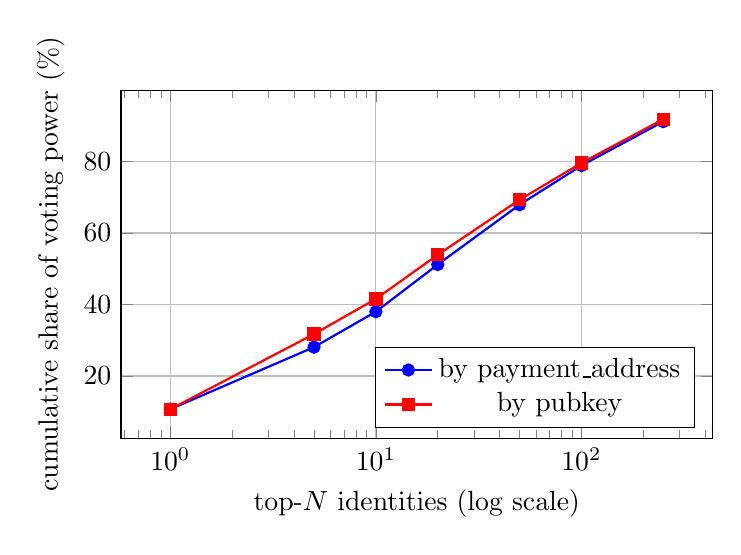
\begin{tikzpicture}
\begin{axis}[
  width=0.75\linewidth, height=6cm,
  xmode=log,
  xlabel={top-$N$ identities (log scale)},
  ylabel={cumulative share of voting power (\%)},
  legend pos=south east,
  grid=major,
]
\addplot[thick, blue, mark=*] coordinates {(1,10.71) (5,28.07) (10,37.99) (20,51.19) (50,67.92) (100,78.88) (250,91.18)};
\addplot[thick, red, mark=square*] coordinates {(1,10.71) (5,31.73) (10,41.56) (20,53.91) (50,69.31) (100,79.60) (250,91.84)};
\legend{by payment\_address, by pubkey}
\end{axis}
\end{tikzpicture}
\caption{Cumulative share of collateral-weighted voting power held by the top-$N$ operator
identities, by two lower-bound proxies. The curve is sampled at the seven $N$ values reported in
Table~\ref{tab:eval-concentration}, not at every $N$. Measured 2026-09-03 at chain height 2,917,115;
data underlying \texttt{paper/\allowbreak{}data/\allowbreak{}concentration\_payment\_address.\allowbreak{}dat} and
\texttt{paper/\allowbreak{}data/\allowbreak{}concentration\_pubkey.\allowbreak{}dat}. \srcmeasured{api.runonflux.io/\allowbreak{}daemon/\allowbreak{}listzelnodes}{2026-09-03}.}
\label{fig:eval-concentration}
\end{figure}

\subsection{Deployed applications}
\label{sec:eval-apps}

This is a measured quantity, \shipped \srcmeasured{api.runonflux.io/\allowbreak{}apps/\allowbreak{}globalappsspecifications}{2026-09-03}.
The endpoint returns \textbf{1,195} application specification records, comprising 1,371 components
(compose entries) and a total of \textbf{7,486} requested instances across all applications.
Instances per application: median 2, mean 6.26, maximum 100, minimum 0; 439 applications (36.7\%)
sit at the platform's 3-instance minimum. Table~\ref{tab:eval-appspec} gives the specification-version
distribution and Table~\ref{tab:eval-registry} the container-registry distribution.

\begin{table}[H]
\centering
\small
\begin{tabular}{lrr}
\toprule
spec version & applications & share \\
\midrule
v2 & 2 & 0.2\% \\
v3 & 27 & 2.3\% \\
v4 & 11 & 0.9\% \\
v5 & 3 & 0.3\% \\
v6 & 70 & 5.9\% \\
v7 & 209 & 17.5\% \\
v8 & 873 & 73.1\% \\
\bottomrule
\end{tabular}
\caption{Application specification version distribution, measured 2026-09-03.
\srcmeasured{api.runonflux.io/\allowbreak{}apps/\allowbreak{}globalappsspecifications}{2026-09-03}. \specv{9} does not yet
appear (\S10).}
\label{tab:eval-appspec}
\end{table}

\begin{table}[H]
\centering
\small
\begin{tabular}{lr}
\toprule
image registry & components \\
\midrule
\texttt{docker.io} (implicit) & 1,332 \\
\texttt{ghcr.io} & 31 \\
\texttt{quay.io} & 3 \\
\texttt{lscr.io} & 2 \\
\texttt{public.ecr.aws} & 1 \\
\texttt{ttl.sh} & 1 \\
\texttt{codeberg.org} & 1 \\
\bottomrule
\end{tabular}
\caption{Container registry distribution across 1,371 components, measured 2026-09-03.
\srcmeasured{api.runonflux.io/\allowbreak{}apps/\allowbreak{}globalappsspecifications}{2026-09-03}.}
\label{tab:eval-registry}
\end{table}

Summed committed resources across all 7,486 requested instances: 8,972.0 vCPU-equivalents,
17,544,229 MB of RAM (17,133.0 GiB), and 160,107 GB of disk. These are the resources declared in
application specifications and enforced at deployment time by the platform's own minimum/maximum
bounds (\texttt{minimum\allowbreak{}Instances}: 3, \texttt{maximum\allowbreak{}Instances}: 100,
\texttt{blocksLasting}: 22,000 blocks per default lifetime,
\srcmeasured{api.runonflux.io/\allowbreak{}apps/\allowbreak{}deploymentinformation}{2026-09-03}) — they are \emph{requested},
not realised. No public endpoint reports realised CPU, memory, disk or network utilisation of the
deployed fleet, and this section does not estimate it (G13); the committed-resource figures above
are the complete measurement available.

Feature usage across the 1,195 applications: \texttt{geolocation} 556 (46.5\%), \texttt{staticip}
50 (4.2\%), \texttt{nodes} (pinned placement) 11 (0.9\%), \texttt{enterprise} 223 (18.7\%),
\texttt{expire} 1,152 (96.4\%), \texttt{owner} 1,195 (100.0\%), \texttt{contacts} 699 (58.5\%),
\shipped \srcmeasured{api.runonflux.io/\allowbreak{}apps/\allowbreak{}globalappsspecifications}{2026-09-03}.

\subsection{Shielded value pools}
\label{sec:eval-shielded}

This is a measured quantity, \shipped \srcmeasured{api.runonflux.io/\allowbreak{}daemon/\allowbreak{}getblockchaininfo}{2026-09-03}.
At chain height 2,917,115, the \texttt{valuePools} field reports a Sapling pool of
\textbf{77,188.75921324 FLUX} and a Sprout pool of \textbf{19,291.17735041 FLUX}, both monitored,
for a combined shielded value of 96,479.93656365 FLUX. Consensus has rejected transparent-to-shielded
transfers since height 835,554 (\srccode{fluxd/\allowbreak{}src/\allowbreak{}main.cpp}{1398--1408}), so both pools have been
closed to new entrants since that height — 2,081,561 blocks before the measurement tip — and every
satoshi in them was shielded before the turnstile closed. Against the total issued supply of
429,466,823.9700 FLUX at height 2,912,015 (\S\ref{sec:eval-supply}), the shielded pools hold
\textbf{0.0225\%} of issued supply (derived). Note count and holder count of either pool are
\textbf{not obtainable} from this or any public endpoint and are not estimated here.

\subsection{Supply, modelled}
\label{sec:eval-supply}

This is a modelled quantity: it reproduces already-shipped \PoN consensus arithmetic
(\srccode{flux-roadmap/\allowbreak{}supply/\allowbreak{}emission\_model.py}{195--243}, itself a transcription of
\PoN's \texttt{Get\allowbreak{}Block\allowbreak{}Subsidy}) rather than a new mechanism, so it is stated \shipped and in
present tense, executed 2026-09-03 by \texttt{flux-\allowbreak{}roadmap/\allowbreak{}supply/\allowbreak{}emission\_model.\allowbreak{}py}
(\srcdoc{flux-roadmap/supply/emission\_model.py, run 2026-09-03}). Current issued supply at height
2,912,015 (mode \texttt{observed}, the model's default and the mode this paper uses for every
current-supply figure) is \textbf{429,466,823.9700 FLUX}. Mode \texttt{code} — a literal
transcription of \texttt{Get\allowbreak{}Block\allowbreak{}Subsidy()} — gives 429,466,973.9700 FLUX at the same height: a
persistent, height-independent offset of exactly \textbf{150.00000000 FLUX}, not the 0.06 FLUX the
model's own docstring claims, traced to a double-counted slow-start block in the \texttt{code}-mode
formula. This discrepancy, its derivation, and the reproduction instructions are given in full in
Appendix~C.

The \PoN subsidy started at \textbf{14 FLUX} per block at activation (height 2,020,000) and is
reduced by a factor of $9/10$ (with per-step integer truncation, so the reduction is not exactly
$0.9^r$) every $\redint = 1{,}051{,}200$ blocks — one year at 30 s spacing — for a maximum of
$\redmax = 20$ reductions (\srccode{flux-roadmap/\allowbreak{}supply/\allowbreak{}emission\_model.py}{149--150}). After the
20th reduction, the subsidy is frozen and does not decay further: at the onset of the tail (height
23,044,000, a 30-second-spacing extrapolation to approximately 2045-10-20; see
\S\ref{sec:eval-threats}), the block subsidy is fixed at 1.70207313 FLUX, and cumulative supply
grows without bound at a constant \textbf{1,789,219.274256 FLUX per year, forever}
(\srccode{flux-roadmap/\allowbreak{}supply/\allowbreak{}emission\_model.py}{514--546}). \textbf{There is no terminal supply.}
Supply at the end of PON year 20 (height 24,095,199, the last block before the flat-rate regime
begins) is 548,043,625.860464 FLUX; this is not a cap, only the point at which the annual emission
\emph{rate} becomes constant. The currently-issued 429,466,823.9700 FLUX is 78.36\% of that
year-20-onset level — a proxy for "how far along" the schedule is, stated explicitly as a proxy
rather than a fraction of a terminal supply, because no terminal supply exists to be a fraction of.
\texttt{MAX\_MONEY} (440,000,000 FLUX) is crossed by cumulative issuance at height 3,730,295
(approximately 2027-06-11); this is not a consensus failure, since \texttt{MAX\_MONEY} bounds a
single transaction's value, never the chain-wide supply accumulator.

\begin{figure}[H]
\centering
\begin{tikzpicture}
\begin{axis}[
  width=0.8\linewidth, height=6.5cm,
  xlabel={year}, ylabel={cumulative issued supply (FLUX)},
  grid=major,
  scaled y ticks=false, yticklabel style={/pgf/number format/fixed, /pgf/number format/1000 sep=\,},
]
\addplot[thick, blue] table[x index=0, y index=2] {../data/emission.dat};
\end{axis}
\end{tikzpicture}
\caption{Cumulative issued FLUX supply, 2026--2060, mode \texttt{observed}. The curve is a
straight line in the flat tail from approximately 2045 onward (1,789,219.274256 FLUX/yr) and never
asymptotes. \srcdoc{flux-roadmap/supply/emission\_model.py, run 2026-09-03}; data in
\texttt{paper/\allowbreak{}data/\allowbreak{}emission.\allowbreak{}dat} (columns: year, height, cumulative\_supply, annual\_emission,
pow\_emission, pon\_emission).}
\label{fig:eval-supply}
\end{figure}

\begin{figure}[H]
\centering
\begin{tikzpicture}
\begin{axis}[
  width=0.8\linewidth, height=6.5cm,
  xlabel={year}, ylabel={modelled annual operator income per node (FLUX/yr)},
  legend pos=north east,
  grid=major,
]
\addplot[thick, blue] table[x index=0, y index=1] {../data/tier_income.dat};
\addplot[thick, red] table[x index=0, y index=2] {../data/tier_income.dat};
\addplot[thick, black] table[x index=0, y index=3] {../data/tier_income.dat};
\legend{Cumulus, Nimbus, Stratus}
\end{axis}
\end{tikzpicture}
\caption{Modelled per-node \PoN issuance income by tier, 2026--2060, at a fixed fleet
(3,246 / 1,615 / 1,627 nodes, held constant; fleet growth and churn are not modelled). Per-node
income scales with tier subsidy share and inversely with tier node count, not with collateral
(\Cref{prop:pnr:across}). \srcdoc{flux-roadmap/supply/emission\_model.py, run 2026-09-03}; data in
\texttt{paper/\allowbreak{}data/\allowbreak{}tier\_income.\allowbreak{}dat} (columns: year, cumulus\_per\_node, nimbus\_per\_node,
stratus\_per\_node, cumulus\_total, nimbus\_total, stratus\_total, total).}
\label{fig:eval-tier-income}
\end{figure}

\subsection{The PNR crossover, modelled, in both denominations}
\label{sec:eval-pnr-crossover}

\PNR does not exist in deployed code. As of the measurement tip (height 2,917,115), the chain is
549,515 blocks short of the planned activation height $\hpa = 3{,}466{,}630$ (approximately
2027-03-12 at 30 s spacing). Everything in this subsection is therefore a \planned projection —
\srcintent{design intake} for the settled design (an 80\%/20\% Foundation/operator
split at activation, ramping by 5 percentage points at each \PoN reduction to a cap of 50\%), and
\srcdoc{scripts/07-pnr-settlement.py, run 2026-09-03} for every number computed from it — and is
stated in future tense throughout. It is stated in both FLUX terms (primary, because FLUX is what
consensus governs) and real terms (secondary, with a price multiple treated as an exogenous axis,
not a forecast); the two must never be used to defend one another. This paper makes no price
prediction anywhere in what follows.

The crossover model uses a fleet fixed at 3,246 / 1,615 / 1,627 nodes (6,488 total) — one Cumulus
node fewer than \S\ref{sec:eval-fleet}'s measured 3,247 / 1,615 / 1,627 (6,489), a one-node
difference between census windows that changes nothing at the precision reported below. It also
uses a \emph{planned} subsidy path distinct from the as-coded schedule of Figure~\ref{fig:eval-supply}:
from $\hpa$, the \PoN subsidy is additionally halved on top of the ordinary $9/10$ reduction
schedule (14 $\to$ 12.6 $\to$ 6.3 FLUX at $\hpa$, then 5.67, 5.103, \ldots), a change that
\texttt{paper/\allowbreak{}data/\allowbreak{}emission.\allowbreak{}dat} does not contain.

\textbf{At activation}, with $\nodeshare(\hpa) = 0.20$ and subsidy 6.3 FLUX, modelled operator
issuance (excluding the dev-fund remainder) would be 6,386,040 FLUX/yr. Under the team's activation-scale
revenue assumption $V_0 = 1{,}431{,}600$ FLUX/yr (1,193 applications $\times$ 100 FLUX/month
$\times$ 12 — a modelling assumption, not a measured receipt total; O17 in \S7), \PNR income would
be $0.20 \times V_0 = 286{,}320$ FLUX/yr. \textbf{\PNR would be 4.29\% of total operator income at
activation} (\PNR as a share of \PoN issuance plus \PNR combined: $286{,}320 / 6{,}672{,}360$).
"Parity" — the point at which \PNR income would equal \PoN issuance income — would require annual
application revenue of \textbf{31,930,200 FLUX/yr}, 22.3$\times$ $V_0$, at activation.

\begin{table}[H]
\centering
\small
\begin{tabular}{lllrrrr}
\toprule
stage start ($\hgt$) & date & subsidy (FLUX) & $\nodeshare$ & operator issuance (FLUX/yr) & parity revenue (FLUX/yr) & growth from $V_0$ \\
\midrule
3,466,630 & 2027-03-12 & 6.3000 & 0.20 & 6,386,040 & 31,930,200 & --- \\
4,122,400 & 2027-10-25 & 5.6700 & 0.25 & 5,747,436 & 22,989,744 & 16.1$\times$ \\
5,173,600 & 2028-10-24 & 5.1030 & 0.30 & 5,172,692 & 17,242,308 & 12.0$\times$ \\
6,224,800 & 2029-10-24 & 4.5927 & 0.35 & 4,655,423 & 13,301,209 & 9.3$\times$ \\
7,276,000 & 2030-10-24 & 4.1334 & 0.40 & 4,189,881 & 10,474,702 & 7.3$\times$ \\
8,327,200 & 2031-10-24 & 3.7201 & 0.45 & 3,770,893 & 8,379,762 & 5.9$\times$ \\
9,378,400 & 2032-10-23 & 3.3481 & 0.50 (cap) & 3,393,803 & 6,787,607 & 4.7$\times$ \\
12,532,000 & 2035-10-23 & 2.4407 & 0.50 & 2,474,083 & 4,948,165 & 3.5$\times$ \\
17,788,000 & 2040-10-21 & 1.4412 & 0.50 & 1,460,921 & 2,921,842 & 2.0$\times$ \\
23,044,000 & 2045-10-20 & 0.8510 & 0.50 & 862,659 & 1,725,319 & 1.2$\times$ (perpetual tail) \\
\bottomrule
\end{tabular}
\caption{Planned \PNR schedule in FLUX terms (primary), modelled 2026-09-03. Dates are 30-second-spacing
extrapolations (\S\ref{sec:eval-threats}). \srcintent{design intake};
\srcdoc{scripts/07-pnr-settlement.py, run 2026-09-03}.}
\label{tab:eval-pnr-flux}
\end{table}

The two levers (falling subsidy, rising $\nodeshare$) would together bring the parity requirement
down from 31.9 M to 6.8 M FLUX/yr over 5.6 years and to 1.7 M FLUX/yr on the perpetual tail. Whether
demand ever reaches that requirement is a separate question, answered only under explicit,
stated assumptions about revenue growth $g$ — never as a forecast. Table~\ref{tab:eval-pnr-growth}
gives the modelled crossover year under six such assumptions ($g \in \{0\%, 10\%, 25\%, 50\%,
100\%, 200\%\}$ per year, constant from $V_0$); these are scenario axes chosen to span a wide
range, not predictions of which growth rate, if any, will occur.

\begin{table}[H]
\centering
\small
\begin{tabular}{lccc}
\toprule
$g$ (per year) & crossover & revenue at crossover (FLUX/yr) & $\nodeshare$ at crossover \\
\midrule
0\% & never & --- & --- \\
10\% & 2038-10 & 4.33 M & 0.50 \\
25\% & 2033-10 & 6.28 M & 0.50 \\
50\% & 2031-10 & 9.33 M & 0.45 \\
100\% & 2030-10 & 17.6 M & 0.40 \\
200\% & 2029-10 & 25.6 M & 0.35 \\
\bottomrule
\end{tabular}
\caption{Modelled crossover year under constant annual revenue growth from $V_0$.
\srcdoc{scripts/07-pnr-settlement.py, run 2026-09-03}; data in \texttt{paper/\allowbreak{}data/\allowbreak{}pnr\_crossover.\allowbreak{}dat}
(columns \texttt{pnr\_g000}\ldots\texttt{pnr\_g200}).}
\label{tab:eval-pnr-growth}
\end{table}

\textbf{Under flat demand ($g = 0\%$), there is no crossover, ever.} The perpetual tail issuance
(862,659 FLUX/yr) exceeds $\nodesharecap \cdot V_0 = 715{,}800$ FLUX/yr, so even at the ramp's cap
of 50\%, \PNR income at flat $V_0$ would never reach \PoN issuance income; the parity requirement
falls over time only because the subsidy keeps falling, and reaching it is a statement about demand
growth, never about the subsidy schedule alone. Sustained growth required to reach parity by a
given year: 134\%/yr by 2029, 73\%/yr by 2030, 47\%/yr by 2031, 32\%/yr by 2032, 25\%/yr by 2033,
16\%/yr by 2035. As scheduled, \PNR would begin as a supplement to operator income; whether it ever
becomes the dominant component is a statement about demand that this paper does not make.

\begin{table}[H]
\centering
\small
\begin{tabular}{lccccc}
\toprule
$g$ \textbackslash\ $m$ & 0.5 & 1 & 2 & 5 & 10 \\
\midrule
0\% & 14.6 & never & never & never & never \\
10\% & 7.6 & 11.6 & 14.6 & 19.6 & 26.1 \\
25\% & 5.6 & 6.6 & 9.6 & 11.6 & 13.6 \\
50\% & 3.6 & 4.6 & 5.6 & 7.6 & 9.6 \\
100\% & 2.6 & 3.6 & 4.6 & 5.6 & 5.6 \\
\bottomrule
\end{tabular}
\caption{Modelled years to \PNR parity, real terms (secondary), under real demand growth $g$
(rows) and an exogenous FLUX price multiple $m$ (columns; $m > 1$ denotes FLUX-price appreciation
against the rebased price table, $m$ is a modelling axis, not a forecast). Under rebasing, price
appreciation \emph{delays} FLUX-terms parity even as real operator income rises — the two
statements are made in different denominations and this paper does not use one to defend the other.
\srcdoc{scripts/07-pnr-settlement.py, run 2026-09-03}; data in
\texttt{paper/\allowbreak{}data/\allowbreak{}pnr\_crossover\_real.\allowbreak{}dat}.}
\label{tab:eval-pnr-real}
\end{table}

\subsection{The drip trade-off}
\label{sec:eval-drip}

This subsection is also \planned and modelled, \srcdoc{scripts/07-pnr-settlement.py, run 2026-09-03},
and supports the settled value \drip = 86,400 blocks (30 days at 30 s spacing) of \S7. The
drip constant $\drip$ trades intra-rotation income spread and activation lag against timing-attack
resistance and pool size. Table~\ref{tab:eval-drip} gives the trade-off at the five candidate values
computed in \texttt{paper/\allowbreak{}data/\allowbreak{}pnr\_drip.\allowbreak{}dat}, against the longest rotation in the fleet (Cumulus,
3,246 nodes in the settlement model).

\begin{table}[H]
\centering
\small
\begin{tabular}{rrrrrr}
\toprule
$\drip$ (blocks) & half-life (days) & decay-side spread$^{\downarrow}$ & one-Stratus recapture & ramp to 95\% (days) & pool at parity (FLUX) \\
\midrule
3,246 & 0.78 & 171.79\% & 0.0205\% & 3.4 & 49,000 \\
10,000 & 2.41 & 38.34\% & 0.0067\% & 10.4 & 152,000 \\
32,460 & 7.81 & 10.51\% & 0.0021\% & 33.7 & 493,000 \\
64,920 & 15.62 & 5.13\% & 0.0010\% & 67.6 & 986,000 \\
\textbf{86,400} & \textbf{20.79} & \textbf{3.83\%} & \textbf{0.00077\%} & \textbf{90} & \textbf{1,310,000} \\
\bottomrule
\end{tabular}
\caption{Modelled drip trade-off at the measured Cumulus rotation length. Decay-side spread is the
first-versus-last-payee income ratio within one Cumulus rotation under zero inflow; recapture is
the fraction of its own \PNR payment a single Stratus node could recover by timing that payment,
against the $10^{-4}$ threshold of requirement H5. Ramp is the time to reach 95\% of steady-state
drip from a zero pool at activation. Pool at parity is the modelled steady-state pool at
parity-scale revenue and $\nodeshare = 0.50$. \srcdoc{scripts/07-pnr-settlement.py, run 2026-09-03};
data in \texttt{paper/\allowbreak{}data/\allowbreak{}pnr\_drip.\allowbreak{}dat}.}
\label{tab:eval-drip}
\end{table}

The settled $\drip = 86{,}400$ would leave one Stratus operator able to recover at most
0.00077\% of its own operator share by timing a payment to its own payout — three orders of
magnitude below the $10^{-4}$ threshold this paper sets for a negligible timing attack — at the
cost of a 20.79-day half-life and a roughly 90-day ramp to steady state after activation, since the
pool is not seeded (settled, O11 in \S7). At parity-scale revenue, the modelled steady-state
pool would hold approximately 1.31 M FLUX; this paper states plainly, per \S7's own framing, that
this balance would be a delay line with a 30-day time constant, not a treasury.

\subsection{Threats to validity}
\label{sec:eval-threats}

The measurements of \S\ref{sec:eval-fleet}--\S\ref{sec:eval-shielded} are a \textbf{single-day
snapshot}, taken 2026-09-03; fleet size, rotation state, application counts and concentration all
change continuously, and no time series is reported here beyond the node-tenure distribution.
Operator-concentration figures (\S\ref{sec:eval-concentration}) are, by construction, \textbf{lower
bounds}: \texttt{payment\_address} and \texttt{pubkey} are the only public identity proxies, and
true concentration by economic party is not obtainable from any public endpoint (G12); this paper
does not claim to know it. Application resource figures (\S\ref{sec:eval-apps}) are
\textbf{requested, not realised}: no public endpoint reports actual CPU, memory, disk, bandwidth or
latency utilisation of the deployed fleet, and none of the committed-resource figures should be
read as a utilisation claim (G13). The supply and \PNR projections of
\S\ref{sec:eval-supply}--\S\ref{sec:eval-drip} assume a \textbf{constant 30-second block spacing}
for every height and date beyond the current tip; the emission model's own validation states this
assumption is accurate to within approximately 0.8 days after 796,820 blocks, and is explicitly
unquantified over the multi-decade horizons (the year-20 tail onset, approximately 2045) that this
section cites — real \PoN spacing may drift, and every calendar date attached to a future height
carries that uncertainty. Finally, the \PNR crossover figures rest on a single, team-supplied
activation-scale revenue assumption ($V_0 = 1{,}431{,}600$ FLUX/yr; O17 in \S7) rather than a
measured receipt total, and the growth rates $g$ and price multiples $m$ used to project beyond it
are modelling axes chosen to span a range, not forecasts of what will occur — this paper makes no
claim about which, if any, will be realised.

%% Drain this section's float queue before the next begins.
\FloatBarrier

\section{Migration and rollout: sequencing, dependencies, and risk}\label{sec:26-migration}\label{sec:migration}

\PoN replaced \PoW at height \hpon, and the transition was not clean: it needed an emergency
reorg-depth override and a checkpoint cluster to stabilize (\S\ref{sec:26-basrate} below). The
roadmap's next transition is not one change but roughly a dozen — \PNR, chain consolidation,
attested hosting, and privacy re-entry — several of which share a load-bearing v9 field, a
consensus-change slot, or a stated precondition that the public roadmap and the design intake do
not always order the same way. This section makes that ordering explicit: which edges the roadmap
states, which this paper infers, and where the two source documents disagree on sequence rather
than on substance. The headline finding is that the riskiest edge in the graph is not a technical
unknown but a sequencing one. \PNR's payoff to hosting is provably zero at the margin
(\S\ref{sec:pnr}), so the mechanism's integrity depends entirely on an eligibility gate that
\S\ref{sec:consensus} and \S\ref{sec:attestation} already show is bound neither to the operator nor
to the machine that passes it. Activating \PNR before hardening that gate is not a parallel
workstream; it is deploying an incentive to defeat a check that does not yet exist. A second,
independent finding — that most of Part~IV waits on three v9 fields with no consumer code today —
makes the v9 enforcement height, since settled at $\hstar = \num{3050000}$
(\S\ref{sec:appspec-v9}), the single most schedule-relevant date in this document.
Everything below is \planned or \vision unless stated otherwise; no date appears here that the
roadmap or the design intake did not state, and quarter labels are reproduced verbatim.

\subsection{The dependency graph}\label{sec:26-depgraph}

Table~\ref{tab:dep-graph} lists dependency edges among the roadmap's chain- and platform-level
items that bear on rollout sequencing, reproduced with the roadmap's own verbatim quarter labels
(\planned; \srcroadmap{flux-roadmap-public.md, dependency edge list, \S3}). Most edges are stated
directly by the roadmap's prose; two are the roadmap's own inferred directionality rather than a
stated gate, and are marked so; one row, previously carried as an open sequencing conflict (C1a), is
now resolved as a simultaneity rather than a precedence and is marked with $=$ rather than $\to$
(\S\ref{sec:26-schedule}); the final row is this section's own argued dependency — it does not
appear in the roadmap's edge list at all — and is discussed in \S\ref{sec:26-precondition} below.

\begin{table}[H]
\centering
\footnotesize
\begin{tabular}{@{}p{5.1cm}p{2.1cm}p{2.0cm}p{3.4cm}@{}}
\toprule
Edge ($A \to B$, $B$ waits on $A$) & Quarter(s) (verbatim) & Status & Source \\
\midrule
\specv{9} spec RFC publication $\to$ \specv{9} rollout & Q4 2026 & stated & \srcroadmap{flux-roadmap-public.md:66} \\
\specv{9} payment-memo field $\to$ PNR v2 (workload-identifying payments) & Q4 2026 $\to$ H1 2027 & stated & \srcroadmap{flux-roadmap-public.md:64,119} \\
\specv{9} \texttt{machineType} flag $\to$ VPS tier & Q4 2026 $\to$ H1 2027 & stated & \srcroadmap{flux-roadmap-public.md:64,125} \\
\specv{9} Duration field $\to$ One balance / auto-renew & Q4 2026 & stated & \srcroadmap{flux-roadmap-public.md:62} \\
Operator protection $\to$ VPS tier launch & Q4 2026 $\to$ H1 2027 & stated & \srcroadmap{flux-roadmap-public.md:125} \\
Bridge redesign (mint-and-burn) $\to$ independent audit (gate before deploy) & Q4 2026 & stated & \srcroadmap{flux-roadmap-public.md:97} \\
Bridge redesign contracts $\to$ attestation / proof-of-reserve work & Q4 2026 & stated & \srcroadmap{flux-roadmap-public.md:99} \\
Q4 2026 bridge attestation work $\to$ attestation network's ``first customer'' & Q4 2026 $\to$ H1 2027 & stated & \srcroadmap{flux-roadmap-public.md:138} \\
PNR v2 testnet $\to$ pilot (CumulusVPN payments) $\to$ mainnet $\to$ per-tier before/after examples published before activation & H1 2027 & stated & \srcroadmap{flux-roadmap-public.md:119} \\
\PNR mainnet activation $=$ parallel-asset mining-reward retirement (simultaneous, at $\hpa$) & roadmap labels H1 2027 / H2 2027 (superseded); resolved date 2027-07-01, with the retiring chains one-directional from March 2027 and shut down in August 2027 (round 34) & resolved: simultaneity, not the roadmap's sequential gate & \srcintent{design intake}, superseding \srcroadmap{flux-roadmap-public.md:133,159} \\
Q4 2026 privacy groundwork (technical/legal/exchange plan) $\to$ chain privacy implementation & Q4 2026 $\to$ H2 2027 & stated & \srcroadmap{flux-roadmap-public.md:102,158} \\
Collateral-maturity proposal $\to$ operator discussion $\to$ activation scheduling, riding an already-planned upgrade & H1 2027 & stated & \srcroadmap{flux-roadmap-public.md:146} \\
Main-chain pruning $\leftrightarrow$ RPC/archive/indexing product & Q3 2026 (product) / H1 2027 (pruning) & inferred (roadmap's own directionality) & \srcroadmap{flux-roadmap-public.md:34,121-122} \\
Attestation hardening (machine-binding the key to the PCR policy already generated) $\to$ \PNR's \emph{ramp} toward $\nodesharecap$ & not dated by the roadmap & inferred (this paper, \S\ref{sec:26-precondition}) & \srcinferred \\
\bottomrule
\end{tabular}
\caption{Dependency edges among roadmap items bearing on rollout sequencing. Quarter labels are
verbatim; ``waits on'' direction is $A \to B$. One row is marked $A = B$ rather than $A \to B$ to
record that the two events are now simultaneous rather than sequential (\S\ref{sec:26-schedule}).}
\label{tab:dep-graph}
\end{table}

\begin{figure}[H]
\centering
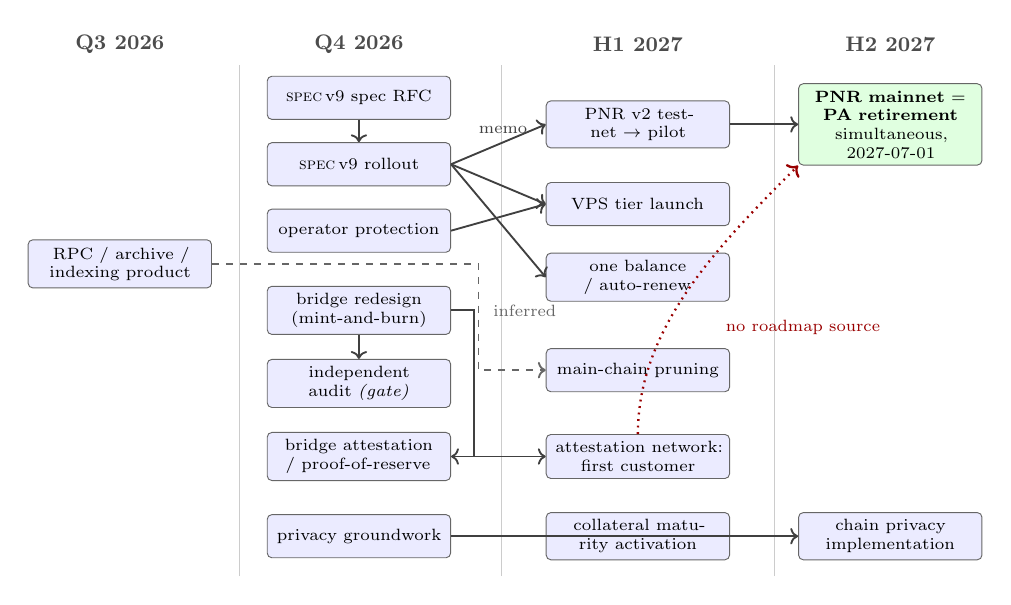
\begin{tikzpicture}[font=\scriptsize,
  n/.style={draw=black!60, rounded corners=2pt, fill=blue!8, align=center, inner sep=3pt,
            text width=2.55cm, minimum height=6.5mm},
  lane/.style={font=\small\bfseries, text=black!70},
  st/.style={->, thick, black!75},
  inf/.style={->, thick, black!60, dashed},
  unc/.style={->, thick, red!60!black, dotted, line width=1pt},
]
\node[lane] at (0,7.4)   {Q3 2026};
\node[lane] at (3.6,7.4) {Q4 2026};
\node[lane] at (7.8,7.4) {H1 2027};
\node[lane] at (11.6,7.4){H2 2027};
\draw[black!20] (1.8,-0.6) -- (1.8,7.1);
\draw[black!20] (5.75,-0.6) -- (5.75,7.1);
\draw[black!20] (9.85,-0.6) -- (9.85,7.1);

% Q3
\node[n] (rpc)  at (0,4.1) {RPC / archive / indexing product};
% Q4
\node[n] (rfc)  at (3.6,6.6) {\specv{9} spec RFC};
\node[n] (v9)   at (3.6,5.6) {\specv{9} rollout};
\node[n] (opro) at (3.6,4.6) {operator protection};
\node[n] (brd)  at (3.6,3.4) {bridge redesign (mint-and-burn)};
\node[n] (aud)  at (3.6,2.3) {independent audit \emph{(gate)}};
\node[n] (att4) at (3.6,1.2) {bridge attestation / proof-of-reserve};
\node[n] (priv) at (3.6,0.0) {privacy groundwork};
% H1
\node[n] (pnr)  at (7.8,6.2) {\PNR{} v2 testnet $\to$ pilot};
\node[n] (vps)  at (7.8,5.0) {VPS tier launch};
\node[n] (bal)  at (7.8,3.9) {one balance / auto-renew};
\node[n] (attn) at (7.8,1.2) {attestation network: first customer};
\node[n] (prun) at (7.8,2.5) {main-chain pruning};
\node[n] (coll) at (7.8,0.0) {collateral maturity activation};
% H2 / resolved
\node[n, fill=green!12] (act) at (11.6,6.2)
  {\textbf{\PNR{} mainnet $=$ PA retirement}\\{\scriptsize simultaneous, 2027-07-01}};
\node[n] (chpr) at (11.6,0.0) {chain privacy implementation};

\draw[st] (rfc) -- (v9);
\draw[st] (v9.east) -- node[above, pos=.55] {memo} (pnr.west);
\draw[st] (v9.east) -- (vps.west);
\draw[st] (v9.east) -- (bal.west);
\draw[st] (opro.east) -- (vps.west);
\draw[st] (brd) -- (aud);
\draw[st] (brd.east) -- ++(0.35,0) |- (att4.east);
\draw[st] (att4.east) -- (attn.west);
\draw[st] (priv.east) -- (chpr.west);
\draw[st] (pnr.east) -- (act.west);
%% The straight rpc->prun line crossed x=3.6 at y=3.36, i.e. through the middle of
%% `brd', and carried its label there. Routed instead along the clear corridor at
%% y=4.1 between `opro' (4.6) and `brd' (3.4), with the label on the vertical leg.
\draw[inf] (rpc.east) -- (5.4,4.1) -- (5.4,2.5) -- (prun.west);
\node[anchor=west, text=black!60] at (5.5,3.4) {inferred};
\draw[unc] (attn.north) .. controls +(0,1.6) and +(-1.2,-1.2) .. (act.south west);
\node[text=red!60!black, anchor=west] at (9.0,3.15) {no roadmap source};
\end{tikzpicture}
\caption{Roadmap dependency graph, oriented by quarter.}
\label{fig:dep-graph}
\end{figure}

\subsection{The edge that shapes the schedule: attestation alongside revenue}\label{sec:26-precondition}

\PNR pays all nodes from a shared fee pool through the \PoN rotation rather than paying the node
that hosts a given application (\planned; \srcintent{design intake}). A node's income is therefore
independent of \emph{which} applications it hosts. That is not free-riding, because an operator
cannot decline placement --- \FluxOS{}'s spawner selects at random from the network-wide list and no
opt-out exists (\shipped;
\srccode{flux/\allowbreak{}ZelBack/\allowbreak{}src/\allowbreak{}services/\allowbreak{}appLifecycle/\allowbreak{}appSpawner.js}{311}) ---
but it does mean \PNR supplies no gradient that rewards hosting well
(\planned; \srcintent{mechanism specification} \srcdoc{reconciliation record}). What compels a node to perform, in this design, is not \PNR — it is the eligibility gate
that lets a node participate in the \PoN rotation in the first place: benchmarking and attestation
(\S\ref{sec:consensus}, \S\ref{sec:attestation}). Those sections already establish that this gate is
weaker than it looks. The benchmark result \fluxd\ accepts is signed by network-wide shared keys
compiled into every copy of \fluxbench, not by a key bound to the operator who ran it (\shipped;
\srccode{fluxd/\allowbreak{}src/\allowbreak{}chainparams.cpp}{233--238}). The attestation key \fluxsas\ produces is derived
by HKDF from static salt and domain values compiled identically into every binary, with no input
that depends on a TPM, on Secure Boot state, or on any other per-machine value (\shipped;
\srcprivate{\SAS{} API server}). Neither signature is bound to the operator or the
machine that produced it.

These two findings compose badly, and the composition has to be sized before it can be turned into a
schedule. Because \PNR raises the value of holding an eligible, paying slot in the rotation, and
because passing the eligibility gate does not currently require possessing the hardware or operator
identity the gate is supposed to attest, \PNR raises the payoff to passing that gate without doing the
work, by exactly what it pays (\planned; \srcdoc{reconciliation record}).

\textbf{By how much is the question, and the answer bounds the conclusion.} At activation \PNR would
pay \num{286320}\flux\ per year. Operator issuance through the same gate at the same height is
\num{6386040}\flux\ per year (\S\ref{sec:pnr}). \PNR would raise the prize by \SI{4.5}{\percent}. An
earlier draft of this subsection concluded from the qualitative composition that hardening attestation
is a \emph{precondition} for \PNR mainnet activation; that conclusion does not survive the
arithmetic, and this paper withdraws it in favour of two statements that do.

\begin{enumerate}
  \item \textbf{Attestation hardening is the schedule's highest-priority security item on its own
  merits.} \SI{95.7}{\percent} of the income flowing through the unbound gate at activation is
  issuance that flows through it today. Treating the work as a \PNR dependency understates its
  urgency by more than an order of magnitude, and invites the reply --- correctly --- that a
  \SI{4.3}{\percent} supplement is not worth blocking a network upgrade for.
  \item \textbf{\PNR's ramp, not its activation, is what should track that work.} $\nodeshare$ rises
  from \num{0.20} to \num{0.50} over six reductions, and each step moves a larger share of operator
  income behind the gate. Coupling the ramp to attestation's completion prices the dependency where
  it actually grows, costs nothing at activation, and does not hand an opponent of \PNR a principled
  veto over it.
\end{enumerate}

What makes the coupling achievable rather than rhetorical is a finding recorded in
\S\ref{sec:attestation}: the image-bound TPM policy the hardening needs is \emph{already generated} on
every capable machine and simply has no consumer. The dependency is therefore not the roadmap's
opt-in bonded network with $k$-of-$n$ challengeable claims (\planned;
\srcroadmap{flux-roadmap-public.md:135-138}), which is a larger and later object, but the narrower
piece of work of binding the attestation key to that policy and serving a verifiable quote. Stated
that way the dependency and \PNR's own March-2027 activation height are compatible; stated as a
dependency on the bonded network, they are not, and the paper would be committing to two things that
conflict. The final row of Table~\ref{tab:dep-graph} is read accordingly.

\subsection{The second critical path: \specv{9}}\label{sec:26-v9}

FluxOS \specv{9} is the second critical path, and it is broader than \PNR alone. \PNR's fee-pool
memo depends directly on the v9 \texttt{paymentMemo} field (\planned; \srcroadmap{flux-roadmap-public.md:64,119}).
Deposited credits depend on the same substrate through the v9 \texttt{duration} field, and both
credits and the provisioning API's spending bounds depend further on a bounded-spending primitive
that \specv{9} does not by itself supply (\planned; \srcdoc{feasibility assessment, rows 1, 11, 14}). The
datacenter tier and the one-provider-runtime convergence depend on the v9 \texttt{machineType} flag
(\planned; \srcroadmap{flux-roadmap-public.md:64,125}; \srcdoc{feasibility assessment, row 21}).

Three of the fields this depends on have zero consumer code anywhere in \FluxOS today:
\texttt{paymentMemo}, \texttt{referralCode}, and \texttt{machineType} (\inprogress;
\srcdoc{reconciliation record}). The orchestration substrate of v9 is built and tested — 932 changed
files and a regression suite of 289 unit-test files running 7,763 test cases on every push
(\inprogress; \srcdoc{reconciliation record}) — but the economic fields the roadmap's own dependency
chain rests on are declared in the schema and unimplemented beneath it. The currently enforced
specification version remains \specv{8}, and 322 of 1{,}195 deployed applications (26.9\%) sit on
six versions older than that (\inprogress; \srcdoc{reconciliation record}; \srcmeasured{network census, \S5}{2026-09-03}).

The v9 enforcement height, settled at $\hstar = \num{3050000}$ (\S\ref{sec:appspec-v9}), is
therefore the most schedule-relevant date in this document (\srcdoc{feasibility assessment}). Meeting it
requires two things that do not exist yet: implemented consumers for the payment-memo, referral, and
machine-type fields, and \texttt{latest\allowbreak{}Supported\allowbreak{}Spec\allowbreak{}Version} raised in lockstep with a fleet-wide
version floor. The mastership/active-standby quorum plane, whose gating field
(\texttt{quorum\allowbreak{}Grant\allowbreak{}Activation\allowbreak{}Height}) is read by production code today but set only in test fixtures
(\inprogress; \srcdoc{reconciliation record}), is deliberately decoupled from $\hstar$ and activates
later, once \specv{9} is stable (\S\ref{sec:appspec-v9}). \settlednote{Partly. \specv{9} activation
and the migration of existing applications are both stated for \textbf{Q4~2026}
\srcintent{design intake}, the enforcement height is $\hstar = \num{3050000}$
\srcintent{design intake}, constrained to follow the economic-field implementation
(\Cref{rem:v9-timing}), and the migration policy is that all applications are migrated automatically
rather than by owner action \srcintent{design intake}. What remains open is the
mechanism by which the 322 applications on legacy versions are rewritten --- an automatic migration
still needs a specified transformation per source version, and none is stated in any artefact read
for this paper.}

\subsection{The privacy prerequisite}\label{sec:26-privacy}

Since height 835{,}554, \fluxd\ rejects any transaction that combines transparent inputs with a
shielded output or joinsplit, with the in-source comment stating the intent directly — the shielded
pool has accepted no new value in approximately 5.4 years (\shipped; \srccode{fluxd/\allowbreak{}src/\allowbreak{}main.cpp}{1398-1408}).
Value can leave the pool ($z \to t$) or move within it ($z \to z$), but it cannot enter.

\textbf{This prerequisite has been withdrawn, not scheduled.} An earlier round of the design intake
recorded that $t \to z$ would be reopened as part of a privacy update, and this paper carried it as a
scheduled dependency for wallet integration and for the payment path of
\S\ref{sec:private-payment}. That has been superseded: the team has decided to \textbf{retire both
shielded pools} rather than reopen either \srcintent{design intake} (\planned).
The reasoning and the schedule are in \S\ref{sec:shielded-retirement}; the consequence for this
section is that reopening leaves the migration path entirely.

Three items therefore leave the dependency graph rather than moving within it: the reopening
activation height, wallet integration for shielded sends in Zelcore and SSP, and the construction in
\S\ref{sec:private-payment} that would have consumed newly-entered value. One item is added: a
sunset height $\hshield = \num{3600000}$ after which shielded spends are invalid, together
with the outreach that must precede it (\S\ref{sec:shielded-retirement}). The roadmap's published direction --- ``we are bringing private
transactions back'' \srcroadmap{flux-roadmap-public.md:167}, and ``chain privacy implementation'' in
H2 2027 \srcroadmap{flux-roadmap-public.md:158} --- is superseded by this decision, and the paper
records the supersession rather than silently reinterpreting the roadmap. What the roadmap says about
not pinning a date on a cryptographic change before its audit is scoped
\srcroadmap{flux-roadmap-public.md:177} still applies, and now applies to a possible \emph{future}
shielded construction (\S\ref{sec:orchard-migration}) rather than to a reopening.

\subsection{The activation schedule}\label{sec:26-schedule}

Table~\ref{tab:activation-schedule} reproduces the design intake's activation schedule: block
height, calendar date, \PoN subsidy $\subsidypon$, and node share $\nodeshare$ through the ramp
toward the cap $\nodesharecap = 50\%$ (\planned; \srcintent{design intake}).

\begin{table}[H]
\centering
\small
\begin{tabular}{@{}lrlrl@{}}
\toprule
Event & Height & Date & Subsidy ($\subsidypon$, \flux) & Node share ($\nodeshare$) \\
\midrule
Current & $\sim$2{,}912{,}015 & 2026-09-03 & 14.0 & --- \\
Reduction 1 ($-10\%$) & 3{,}071{,}200 & 2026-10-25 & 12.6 & --- \\
PA Depletion ($-50\%$), $\hpa$ & \textbf{3{,}787{,}502} & \textbf{2027-07-01} & \textbf{6.3} & \textbf{20\% --- \PNR begins} \\
Reduction 2 ($-10\%$) & 4{,}122{,}400 & 2027-10-25 & 5.67 & 25\% \\
Reduction 3 ($-10\%$) & 5{,}173{,}600 & 2028-10-24 & 5.103 & 30\% \\
annually thereafter & $+1{,}051{,}200$ & --- & $\times 0.9$ & $+5$pp \\
\bottomrule
\end{tabular}
\caption{\PNR activation schedule from the design intake. PA Depletion ($\hpa$) is simultaneous with
the parallel-asset mining-reward cut and the swap contract taking effect
(\S\ref{sec:26-schedule}; \srcintent{design intake}), not a half-year ahead of it as
the public roadmap's superseded sequencing would have had it. Node share $\nodeshare$ ramps to a
declared cap $\nodesharecap = 50\%$, reached around 2033 on the stated annual step
(\srcintent{design intake}).}
\label{tab:activation-schedule}
\end{table}

\PNR activation and the parallel-asset emission cut occur at the \emph{same} event: height
$\hpa = 3{,}787{,}502$, 2027-07-01, is when the node share $\nodeshare$ first becomes nonzero and when
parallel-asset mining-reward emission is cut (\planned; \srcintent{design intake}). This resolves what
earlier drafts of this paper carried as an open sequencing conflict (C1a). The public roadmap had
stated a different, sequential plan — ``retirement of any parallel asset's mining rewards comes only
after PNR v2 is demonstrably paying operators'' and, more specifically, ``parallel-asset mining
retirement — only after PNR v2 is paying operators on mainnet, announced at least 90 days ahead'' — a
step the roadmap placed in H2 2027, one half-year after PNR v2's own H1 2027 slot
(\srcroadmap{flux-roadmap-public.md:133,159}). That sequencing is \textbf{superseded} by the team's
direct answer to this paper: activation is simultaneous, at $\hpa$ (\planned;
\srcintent{design intake}). This section and \S\ref{sec:parallel-assets} both now
describe one coordinated transition rather than two phases separated by an interval.

The consequence is not merely notational. The roadmap's sequential design existed to create a
checkpoint: a proving period, of up to a stated half-year with 90 days' advance notice, in which
\PNR could be observed actually paying operators before the parallel assets whose retirement it was
meant to justify were cut. With simultaneous activation, that checkpoint does not exist —
deliberately, by the team's own later decision, not by oversight. \S\ref{sec:26-risk} carries this as
a named risk rather than treating the superseded roadmap language as still in force.

\subsection{An empirical base rate for consensus change}\label{sec:26-basrate}

The transition this paper's thesis rests on was not clean, and the fact belongs in a risk analysis
rather than a footnote. \fluxd's normal reorg-depth limit, \texttt{MAX\_REORG\_LENGTH}, is 40
blocks, but it was overridden to 5{,}000 for the height range $[2{,}020{,}000,\ 2{,}025{,}000]$, an
override the source comments describe as a ``[t]emporary deep reorg limit during PON stabilization
period'' (\shipped; \srccode{fluxd/\allowbreak{}src/\allowbreak{}main.cpp}{8983-8988}). Alongside it sits a checkpoint cluster
at heights 2{,}020{,}500 / 2{,}021{,}000 / 2{,}021{,}500 / 2{,}022{,}000 / 2{,}029{,}000, labelled in
the source ``PON activation and stabilization checkpoints -- EMERGENCY FORK RECOVERY'' (\shipped;
\srccode{fluxd/\allowbreak{}src/\allowbreak{}chainparams.cpp}{277-283}). The \PoW$\to$\PoN transition, in other words, required
active emergency intervention after activation despite having been planned.

The roadmap itself draws two lessons from this kind of history, applied prospectively to the next
consensus change it proposes (collateral maturity): first, that a proposal should ride an
already-planned network upgrade rather than force its own — ``it would ride an already-planned
network upgrade rather than forcing its own'' (\planned; \srcroadmap{flux-roadmap-public.md:146});
second, that proposals go to operators for discussion before any activation is scheduled, not after
— stated for collateral maturity (\srcroadmap{flux-roadmap-public.md:146}) and echoed in \PNR's own
staged sequence, which ends with ``per-tier before-and-after examples published to operators before
activation'' (\planned; \srcroadmap{flux-roadmap-public.md:119}). Three further consensus-adjacent
changes are queued behind \PoN and sit in \S\ref{sec:chain-ops}: main-chain pruning (\planned;
\srcroadmap{flux-roadmap-public.md:121-122}), collateral maturity (\planned;
\srcroadmap{flux-roadmap-public.md:143-146}), and the post-quantum migration roadmap (\planned;
\srcroadmap{flux-roadmap-public.md:148-149}) — the last of which the roadmap is explicit is a
multi-year effort beyond publishing a path. Against the C16 base rate, this is why sequencing them
into as few network upgrades as possible matters: each additional independently-forced consensus
change is, by the network's own recent history, an occasion on which stabilization measures of the
kind seen at \PoN activation may again be needed.

\subsection{Risk register}\label{sec:26-risk}

Table~\ref{tab:risk-register} lists the risks this section's dependency analysis surfaces, the
mechanism each threatens, the evidence behind its likelihood, and the mitigation that exists or does
not.

%% longtable rather than table[H]: the [H] tabular ran 272pt past the text block (log: overfull
%% vbox), so its last row was cut and its caption never rendered. Same header pattern as Appendix B.
\begingroup
\footnotesize
\begin{longtable}{@{}p{2.9cm}p{2.1cm}p{4.3cm}p{3.6cm}@{}}
\caption{Risk register for the sequencing and dependencies described in this section.}
\label{tab:risk-register}\\
\toprule
Risk & Threatens & Likelihood basis (evidence) & Mitigation \\
\midrule
\endfirsthead
\multicolumn{4}{l}{\small\itshape (Table~\ref{tab:risk-register} continued)}\\
\toprule
Risk & Threatens & Likelihood basis (evidence) & Mitigation \\
\midrule
\endhead
\bottomrule
\endfoot
Demand growth undershoots; \PNR stays a supplement & \PNR (\S\ref{sec:pnr}) &
At $\hpa$, parity needs $\sim$31.9M\flux/yr (\S\ref{sec:eval-pnr-crossover}) against assumed demand
of $\sim$1.43M\flux/yr (the team's assumption of 1{,}193 applications at 100\flux/month; the census
counts 1{,}195 applications and 7{,}486 instances, \S\ref{sec:eval-apps}); \PNR is $\sim$4.3\% of
operator income at activation; under flat demand there is no crossover, ever (\srcintent{design intake};
\srcdoc{reconciliation record}) &
Ramp lowers the parity threshold to $\sim$6.8M\flux/yr by 2032-10, $\sim$5.6 years post-$\hpa$
(\S\ref{sec:eval-pnr-crossover}); no stated policy if demand still undershoots (O13, open) \\
\addlinespace
Simultaneous activation removes the roadmap's proving-period checkpoint & \PNR credibility;
parallel-asset retirement (\S\ref{sec:pa-sequencing}, \S\ref{sec:26-schedule}) &
\PNR activation and the parallel-asset emission cut are simultaneous at $\hpa = 3{,}787{,}502$
(\srcintent{design intake}), superseding the roadmap's plan to retire parallel
assets only after \PNR is ``demonstrably paying operators,'' announced 90 days ahead
(\srcroadmap{flux-roadmap-public.md:133,159}) &
None stated; a deliberate simplification by the team, not an oversight, but it means no external
observer can verify \PNR is paying operators before the parallel assets it justifies retiring are cut \\
\addlinespace
Eligibility-gate exploitation once \PNR pays & \PNR's only hosting compulsion (\S\ref{sec:consensus},
\S\ref{sec:attestation}) &
Benchmark keys are shared constants, not per-operator (\srccode{fluxd/\allowbreak{}src/\allowbreak{}chainparams.cpp}{233--238});
attestation key derivation has no machine-bound input (\srcprivate{\SAS{} API server});
\PNR{} adds no gradient rewarding good hosting (\srcdoc{reconciliation record}), though it adds only
\SI{4.5}{\percent} to a payoff the same gate already carries &
Machine-binding the attestation key to the PCR 4/7/11 policy \ArcaneOS{} already generates
(\S\ref{sec:attestation}) --- narrower and nearer than the roadmap's opt-in bonded network, k-of-n,
planned H1 2027 (\srcroadmap{flux-roadmap-public.md:135-138}); \S\ref{sec:26-precondition} couples it
to \PNR's ramp rather than blocking activation on it \\
\addlinespace
A bridge audit finding delays consolidation & Bridge redesign, chain consolidation (\S\ref{sec:bridge}) &
Audit is an explicit hard gate before deploy (\srcroadmap{flux-roadmap-public.md:97}); the network's
only prior consensus-adjacent transition needed emergency intervention despite planning
(\S\ref{sec:26-basrate}) &
Audit-before-deploy is itself the stated mitigation; no contingency schedule exists for a finding
that requires rework (open) \\
\addlinespace
\specv{9} migration strands legacy applications & \PNR, credits, provisioning API, datacenter tier
(\S\ref{sec:26-v9}) &
322 of 1{,}195 deployed applications (26.9\%) sit on six versions older than \specv{8}
(\srcdoc{reconciliation record}; \srcmeasured{network census, \S5}{2026-09-03}); the enforcement
height is settled at $\hstar = \num{3050000}$ but no per-version transformation or eviction
policy exists &
Forced automatic migration at $\hstar$ \srcintent{design intake}; the
transformation per source version is unspecified (\S\ref{sec:26-v9}) \\
\addlinespace
Moderation-quorum capture event & Content-reporting quorum (\S\ref{sec:governance}) &
4 owner identities (\texttt{payment\_address}) reach the 25\% eviction threshold, falling to 3 once addresses linked by a shared node key or collateral funding transaction are merged; the largest holds 10.71\% of collateral-weighted
voting power; Gini 0.8375 (\srcmeasured{network census, \S2}{2026-09-03}; \srcdoc{reconciliation record}) &
Two-chamber rule (weight threshold plus distinct-identity count with tenure) raises the cost of a
surprise capture but does not lower $\kappa$; does not reach censorship resistance (\srcdoc{reconciliation record}) \\
\addlinespace
Shielded-pool sunset destroys notes not swept in time & Holders of the 96{,}479.94\flux{} still in
the pools (\S\ref{sec:privacy}, \S\ref{sec:shielded-retirement}) &
$t \to z$ closed since height 835{,}554, approximately 5.4 years (\srccode{fluxd/\allowbreak{}src/\allowbreak{}main.cpp}{1398-1408});
reopening is cancelled and both pools are to be retired
(\srcintent{design intake}); roadmap will not pin a date on a cryptographic
change before its audit is scoped (\srcroadmap{flux-roadmap-public.md:177}) &
Sunset settled at $\hshield = \num{3600000}$ (2027-04-27), announced at publication and \num{187502} blocks before $\hpa$
(\srcintent{design intake}); ZIP-209 turnstile enforcement active for the window
and direct holder outreach are this paper's recommendations, not confirmed decisions
(\S\ref{sec:shielded-retirement}) \\
\addlinespace
Archival capacity becomes demand-dependent once history is a paid product & Pruning, archive/RPC/indexing
(\S\ref{sec:chain-ops}, \S\ref{sec:managed-services}) &
Roadmap pairs the Q3 2026 archive product directly with H1 2027 pruning, but states the direction
loosely and marks it \srcinferred\ in its own dependency list rather than as a strict gate
(\srcroadmap{flux-roadmap-public.md:34,121-122}) &
None stated; if the archive product does not attract paying demand, the operator incentive to run
archive nodes once pruning removes the default full-history requirement is untested \\
\end{longtable}
\endgroup

\subsection{What would have to be true}\label{sec:26-conditions}

This is not a schedule with a confidence interval attached; it is a set of conditions, stated
explicitly, under which the sequencing above resolves into a working rollout rather than a stalled
or exploited one.

\begin{itemize}
\item \textbf{Demand, not price, must grow.} The number of deployed applications, instances, and
resources sold must grow roughly in line with the compounding schedule in
Table~\ref{tab:activation-schedule} for \PNR to become more than a $\sim$4\% supplement to operator
income; this is a claim about deployment counts and resources sold, never about price
(\srcintent{design intake}; \srcdoc{reconciliation record}).
\item \textbf{Attestation hardening must precede or coincide with \PNR mainnet activation, not
follow it.} If the bonded attestation network is not operational by the time \PNR begins paying
operators, the eligibility gate — already shown not to be operator- or machine-bound
(\S\ref{sec:26-precondition}) — becomes a directly monetized target rather than a weak but
unexploited assumption.
\item \textbf{\specv{9}'s three economic fields need implemented consumers before any of their
dependents activate.} \texttt{paymentMemo}, \texttt{referralCode}, and \texttt{machineType} must
each acquire consumer code, and \texttt{latest\allowbreak{}Supported\allowbreak{}Spec\allowbreak{}Version} must rise in lockstep with a
fleet-wide version floor, before \PNR,
credits, the provisioning API's bounds, or the datacenter tier can activate on the schedule the
roadmap implies (\srcdoc{reconciliation record}).
\item \textbf{The shielded-pool sunset must be executed as settled.} Reopening $t \to z$ is cancelled and
both pools are to be retired \srcintent{design intake}; what replaces the old open
question is a sunset height $\hshield = \num{3600000}$, confirmed
\srcintent{design intake}, together with ZIP-209 turnstile enforcement for the
drain-only window and the direct outreach preceding it, both this paper's recommendations
(\S\ref{sec:shielded-retirement}, \S\ref{sec:26-privacy}).
\item \textbf{The removed proving period is an accepted risk, not an oversight, and should stay
visible.} Simultaneous activation (\S\ref{sec:26-schedule}) means no external observer can confirm
\PNR pays operators before parallel-asset mining rewards are retired; any activation announcement
should say so rather than let a reader assume the roadmap's original 90-day-notice checkpoint still
applies.
\item \textbf{Consensus changes need to be batched into as few network upgrades as possible},
following the roadmap's own stated preference to ride an already-planned upgrade rather than force a
new one; every additional independently-forced consensus change is, by the measured base rate of the
\PoW$\to$\PoN transition, an occasion on which unplanned stabilization measures may again be needed
(\S\ref{sec:26-basrate}).
\item \textbf{The bridge audit and the moderation quorum's residual capture risk need to be treated
as live constraints, not formalities}, since neither has a stated contingency for an adverse finding
or a captured vote (Table~\ref{tab:risk-register}).
\end{itemize}

%% Drain this section's float queue before the next begins.
\FloatBarrier

\section{Related work}\label{sec:related-work}

\Flux's claim in this paper is architectural, not comparative marketing: a network in which an
autonomous agent can rent capacity, pay for it, and leave, without an account, a payment card, or a
human in the loop, using an operator set that is capital-bonded and enumerable rather than merely
reputational. Positioning that claim requires comparing mechanisms, not brands. This section takes
each mechanism the paper specifies elsewhere — a decentralized resource market, a consensus protocol,
a bridge, an attestation root, a shielded payment pool, a delegation primitive, and a machine-facing
interface — and states the prior art for that mechanism specifically, what \Flux inherits from it, and
where \Flux's design departs. Claims about other systems describe only what those systems have
published, with no maturity judgement about their roadmaps; claims about \Flux itself carry the same
maturity and provenance discipline as the rest of this paper.

\subsection{Decentralized compute markets}

Akash \citep{akash} and Golem \citep{golem} are open compute marketplaces: a tenant posts a resource
request, providers bid or advertise matching capacity, and a match is made without the marketplace
itself verifying that a provider's declared hardware exists or performs as advertised; both settle
payment in the network's own token, escrowed from the tenant and released to the winning provider over
the deployment's life. Render \citep{render} and io.net \citep{ionet} apply the same open-bidding
structure to a single resource class — GPU rendering and GPU compute for machine-learning workloads,
respectively — aggregating capacity from an unbonded, self-reported pool of node operators. Aethir
\citep{aethir} targets the same GPU-cloud niche with an enterprise framing. In all five, the trust a
tenant extends to a provider is reputational: nothing in the protocol requires a provider to lock
capital against non-delivery, and nothing verifies a provider's declared specification beyond the
provider's own attestation of it.

\Flux departs from this class in one specific way: every \FluxNode operator posts a tier-scaled
collateral that consensus checks against the registration transaction before a node is eligible to run
anything \shipped\ \srccode{fluxd/\allowbreak{}src/\allowbreak{}coins.cpp}{630--686}, and the resulting registry is directly
enumerable from chain state — 6{,}489 records at the most recent measurement \shipped\
\srcmeasured{api.runonflux.io/\allowbreak{}daemon/\allowbreak{}listzelnodes}{2026-09-03}. Two properties follow that an open,
self-reported marketplace cannot offer by construction. First, the same registry that gates eligibility
is what \PoN's block-production sortition ranks and rotates \shipped\
\srccode{fluxd/\allowbreak{}src/\allowbreak{}pon/\allowbreak{}pon-minter.cpp}{78--104}, and it is the substrate §7's fairness argument for
revenue-funded compensation is built on \planned\ \srcintent{§7}. Second, an enumerable operator set is
a tractable target for a future key migration in a way an open, unbonded pool cannot be: collateral is
already a registered set on \Flux, so a migration that starts there is a narrower problem than a
general UTXO migration \vision\ \srcintent{feasibility assessment}. This is also what makes the resulting
eviction quorum Sybil-resistant by construction \citep{douceur2002sybil} — a property §23 relies on and
this section returns to below. Neither property is free: collateral is capital locked against no
guaranteed return, and an enumerable registry is also a measurably concentrated one — the largest single
collateral-weighted identity in the registry holds 10.71\% of voting power across 237 Stratus nodes
under one key \shipped\ \srcmeasured{api.runonflux.io/\allowbreak{}daemon/\allowbreak{}listzelnodes}{2026-09-03}, a fact §23 uses
directly.

\subsection{Hyperscalers}

Hyperscale clouds occupy an adjacent but distinct point in the design space, and there is no hostility
in stating the difference plainly. They price by metered consumption rather than by reservation, offer
deep managed-service catalogs, and back regional deployments with contractual latency and availability
guarantees; none of that is disputed here \citep{wust2018blockchain}. What \Flux offers that a
hyperscaler does not is orthogonal rather than superior: no account, no payment card, and no human
approval step stand between a payment and a running deployment — already true, concretely, of
\CumulusVPN's entitlement path, where a WireGuard public key is itself the credential and no
server-issued account exists \shipped\ \srccode{cumulusvpn/\allowbreak{}gateway/\allowbreak{}internal/\allowbreak{}entitle/\allowbreak{}entitle.go}{218--287}
— and the operator fulfilling the deployment is drawn from the capital-bonded, enumerable set described
above rather than an opaque corporate fleet. Concretely, \Flux prices a reservation: a deployment's
price is a function $\price(\resvec,\ninst,\dur)$ of a resource vector, an instance count and a duration fixed at request time,
not a metered function of realized usage \shipped\
\srccode{flux/\allowbreak{}ZelBack/\allowbreak{}src/\allowbreak{}services/\allowbreak{}utils/\allowbreak{}appUtilities.js}{89--134}
\srcmeasured{api.runonflux.io/\allowbreak{}apps/\allowbreak{}deploymentinformation}{2026-09-03} (§16). That is the architectural
difference that matters more than any feature count: a reservation price is settled once, at deployment
time, and the only subsequent dispute surface is whether the reserved resources were delivered, not how
much of them was consumed.

\subsection{Storage and content networks}

Filecoin \citep{filecoin2017} and IPFS \citep{benet2014ipfs} are the closest prior art for hosting
rather than compute. Filecoin's storage deals are prepaid by the client and backed by provider-posted
collateral that the protocol can slash if the provider fails to prove continued possession of the
stored data; the remedy for non-performance is financial, enforced against the provider's own stake.
\Flux's stated remedy for a host that fails to deliver a paid-for deployment is different in kind:
replacement rather than refund — the network moves the workload to another eligible host rather than
returning payment to the tenant \planned\ \srcintent{§16}. IPFS carries no equivalent mechanism at
either layer: content addressing guarantees that a hash resolves to the bytes it names, but the network
has no built-in remedy for a bad actor and no protocol-level way to remove content once published —
persistence is a function of who chooses to pin it, not of any consensus process. \Flux's proposed
content-reporting quorum (§23) is the opposite kind of mechanism: a collateral-weighted vote to evict a
specific application from the fleet \planned\ \srcintent{§23}. Placed side by side, the three positions
are distinct: Filecoin slashes a provider's stake for failing to keep data available; IPFS has no
mechanism to make content unavailable at all; \Flux's quorum is built expressly to make a specific
application unavailable network-wide, which is not the same problem as either.

\subsection{Consensus}

\PoN replaces Bitcoin-style proof of work \citep{nakamoto2008bitcoin} with collateral-gated sortition
over the \FluxNode registry described above: eligibility to produce the next block is a function of
tier and collateral rather than of hashing power. The precise point a reader should not have to infer
is in the fork-choice rule. Every \PoN block contributes a fixed chainwork value of $2^{40}$ regardless
of its actual difficulty target \shipped\ \srccode{fluxd/\allowbreak{}src/\allowbreak{}pow.cpp}{284--290}, so fork choice is not a
race for the chain with the most accumulated work in the sense Nakamoto consensus assumes
\citep{nakamoto2008bitcoin} and the security analyses built on that assumption use
\citep{gervais2016security,eyal2014majority} — it is a block-count race, resolved by which chain
extended first and furthest. That places \PoN's security argument closer to proof-of-stake sortition
schemes such as Algorand \citep{gilad2017algorand}, which likewise select a block producer by a
verifiable, stake-weighted draw rather than by cumulative work, than to Nakamoto consensus or to
chain-based proof-of-stake protocols such as Ouroboros \citep{kiayias2017ouroboros} that still
accumulate a work-like quantity along the chain \srcinferred. Two differences from Algorand are worth
stating rather than eliding: \PoN's eligibility draw is public and registry-based rather than a private
per-round cryptographic sortition, and, so far as the material available to this paper shows, \PoN has
no finality gadget layered over its fork-choice rule, unlike systems that pair a longest-chain-style
base protocol with an explicit finality overlay \citep{buterin2017casper} \srcinferred.
\citep{bonneau2015sok} frames exactly this kind of comparison — what a consensus protocol's security
argument actually rests on, rather than which family it is conventionally filed under — and is the
right lens for reading \PoN this way.

\subsection{Bridging}

Cross-chain interoperability designs separate broadly into light-client verification, trusted or
federated attestation, and atomic exchange of assets that already exist on both chains
\citep{zamyatin2021sok}. IBC \citep{cosmosibc} is the clearest instance of the first category: a
receiving chain runs a light client of the sending chain, verifying block headers and validator
signatures directly, so no third party is trusted beyond the sending chain's own consensus. XCLAIM
\citep{zamyatin2019xclaim} generalizes the idea to chains, like Bitcoin, that cannot be light-client
verified cheaply on the receiving side, using over-collateralized vaults and SPV-style proofs instead.
CCTP \citep{cctp} sits in the second category: an attestation service observes a burn on the source
chain and signs a message authorizing a mint on the destination chain, substituting a designated
attester for a light client. Atomic swaps \citep{herlihy2018atomic} sit outside both categories: they
exchange assets that already exist on both chains using hashed time-locks, but they cannot
\emph{issue} an asset on a chain where it does not yet exist.

Neither of the first two categories is presently constructible for \Flux, and the reason is the header,
not the will. A light client needs three things \PoN's header does not give it. First, per the bridge
design's own analysis, the header carries no commitment to the \FluxNode registry, so a verifier cannot
check that a block's signer was an eligible operator without holding the full registry itself \planned\
\srcintent{mechanism specification}. Second, chainwork is fixed at $2^{40}$ per block regardless of
difficulty \shipped\ \srccode{fluxd/\allowbreak{}src/\allowbreak{}pow.cpp}{284--290}, so there is no cumulative-work quantity a
light client could use to prefer one candidate chain over another the way an SPV client does. Third, a
2-of-4 emergency key set can produce a valid block outside \PoN's normal eligibility rule, with no time
or stall-detection gate on when it may act \shipped\ \srccode{fluxd/\allowbreak{}src/\allowbreak{}emergencyblock.cpp}{183--191}, so no
light-client rule derived from \PoN eligibility alone would be sound even if the first two problems were
solved. The consequence is concrete: the most trust-minimized bridge architecture available to
IBC-style systems is closed to \Flux until the header changes to commit to the registry, and that is a
consensus change, not a bridge-layer one, and a candidate for the same network upgrade that would carry
collateral maturity \planned\ \srcintent{§8}.

Atomic swaps do not fill this gap either, for a reason independent of the header: a swap exchanges FLUX
that already exists on \Flux for an asset that already exists on the destination chain. It cannot mint
FLUX on a chain where none yet exists, which is exactly what parallel-asset issuance requires \planned\
\srcintent{mechanism specification}. Swaps are the right primitive for \FusionX's exchange product, where
both assets already exist on both sides; they are not a candidate for the bridge itself. \Flux's
remaining option, and the one §22 specifies, is canonical mint-and-burn under a bonded, capped
custodian — closer to CCTP's trusted-attester model than to IBC's light client, with per-chain caps
$\bcap{c}$ and reserve slack $\bslack = \breserve - \sum_c \bminted{c}$ (§22) doing the work a light
client would otherwise do \planned\ \srcintent{§22}.

\subsection{Attestation and bonded assertions}

ArcaneOS's measured boot and Secure-Boot platform-key pinning \shipped\ \srccode{fluxsas/\allowbreak{}src/\allowbreak{}fes/\allowbreak{}fes.cpp}{70--81},
its dm-verity root-hash verification \shipped\ \srcprivate{\SAS{} watchdog}, and its
LUKS-backed disk encryption \shipped\ \srcprivate{\SAS{} disk encryption} do real work
against a remote attacker without any special hardware trust anchor. The question this section
positions is not whether that machinery works but what the resulting attestation is rooted in. One line
of prior art roots attestation in silicon: Intel SGX \citep{costan2016sgx} ties an attestation to a
hardware-manufacturer-signed key that a remote verifier can check without trusting the party running
the enclave. A second line roots it in capital: EigenLayer \citep{eigenlayer} lets operators post
slashable stake against off-chain assertions, so an assertion is trusted because a bond would be lost
if it is false, not because of where it was computed. \Flux's planned attestation network is a version
of the second model — a bond rather than a chip is what would secure the claim that a machine booted a
particular image \planned\ \srcroadmap{new benchmark tool, signed node attestation,
timeline.html:295--296}.

The honest state of the current system is that neither model is yet in place. The \fluxsas signing key
for the default, \texttt{cdn}, \texttt{mesh} and \texttt{app} attestation purposes is derived from
static salt and domain values compiled identically into every binary; none of its inputs depends on TPM
state, Secure Boot state, or any other per-machine value \shipped\
\srcprivate{\SAS{} API server}. What that attestation demonstrates is that the signer
holds a value shipped in every copy of the software, not that a particular machine booted a particular
image. The trust root behind "this node booted something \Flux considers legitimate" is today entirely
\Flux-operated, composed of the platform key above and a pair of \Flux-operated web services publishing
allowed dm-verity root hashes that the watchdog polls roughly daily and treats as secure if unreachable
\shipped\ \srcprivate{\SAS{} watchdog}. Neither SGX's hardware root nor EigenLayer's
economic root is present yet; the \texttt{purpose=\allowbreak{}mesh} attestation type already compiled into
\fluxsas with no consumer \shipped\ \srcprivate{\SAS{} API server} is the stated seed of
the bonded design that would supply one \planned\ \srcintent{§14}.

\subsection{Privacy}

\Flux's shielded pool is Sapling — encrypted notes, a note commitment tree $\tree$, nullifiers $\nf$,
and Groth16 proofs \citep{groth2016size} verifying spend and output statements over $\zaddr$-typed
value — specified by the Zcash protocol \citep{zcashprotocol} and tracing to the original Zerocash
construction \citep{bensasson2014zerocash}, and it is live on-chain today \shipped\
\srccode{fluxd/\allowbreak{}src/\allowbreak{}main.cpp}{1398--1408}. The trusted setup behind those proofs was produced by a
multi-party ceremony in the random-beacon model \citep{bowe2017mpc}; a newer construction removing the
need for any such ceremony exists in the literature \citep{bowe2019halo} but has not been ported into
\Flux's shielded pool, which remains on Sapling and Groth16 \shipped\ \srccode{fluxd/\allowbreak{}src/\allowbreak{}main.cpp}{1450--1468}.

\textbf{The comparison changes direction going forward.} Both pools are to be retired
(\S\ref{sec:shielded-retirement}), so \Flux{} is moving \emph{away} from the Zcash lineage on this
axis while the systems it is compared against move toward stronger privacy. The resulting position is
unusual and should be stated as such rather than blurred: on settlement privacy \Flux{} will be
comparable to Bitcoin rather than to Zcash, and weaker than every privacy-focused chain in this
survey. What it gains is a consensus layer with no proving system, no trusted-setup inheritance and
no unenforced turnstile --- a smaller and more auditable object, which is the trade the team has
chosen \srcintent{design intake}.
None of this machinery is \Flux's invention, and this paper does not claim otherwise: the cryptography,
the setup, and the protocol are inherited in full.

Where \Flux does make an original decision is consensus policy, not cryptography: since height
835{,}554, the same consensus path cited above rejects any transaction that mixes a transparent input
with a shielded output or joinsplit, closing the pool to new value from the transparent side \shipped\
\srccode{fluxd/\allowbreak{}src/\allowbreak{}main.cpp}{1398--1408}. Value already inside the pool can still move
$\zaddr\to\zaddr$ or leave $\zaddr\to\taddr$, but nothing enters; the pool's value has been
monotonically non-increasing for approximately 5.4 years, holding 77{,}188.76 FLUX in Sapling and 19{,}291.18 FLUX in
Sprout at last measurement \shipped\ \srcmeasured{fluxd chain tip 2{,}917{,}115}{2026-09-03}. That
single fact reorders how privacy commitments elsewhere should be read: reopening the pool would have
been a consensus change and the prerequisite for every downstream privacy item, not a
wallet-integration task --- and it is now cancelled in favour of retirement (\S\ref{sec:shielded-retirement}).

Payment channels are the other well-known route to transactional privacy — Lightning
\citep{poon2016lightning} keeps individual payments off-chain entirely, trading on-chain settlement for
a channel-liquidity trust assumption. \Flux does not take this route for deployment payment; §16 works
over on-chain transparent settlement and §21 was specified over on-chain shielded settlement \srcintent{§16}, so a channel network's
liquidity and routing assumptions are not this paper's problem, but neither is its privacy benefit
available for free. The specific problem §21 identifies is narrower and, so far as this corpus
establishes, open: proving that a shielded payment funds a \emph{particular} deployment without
revealing which one is hard precisely because an application's address is itself a workload identifier,
so a spend statement naming that address defeats the purpose of hiding it \vision\
\srcintent{feasibility assessment}. This has the shape of a blind-credential problem — proving membership
in, or payment toward, a class without revealing which member —
and the relevant literature is well developed: blind signatures \citep{chaum1982blind},
anonymous credentials \citep{camenisch2001credentials}, compact e-cash
\citep{camenisch2005ecash}, anonymous authorization tokens \citep{privacypass}, and
zero-knowledge group membership with per-epoch nullifiers \citep{semaphore}. What none of it
supplies directly is the combination \S\ref{sec:private-payment} needs: a public obligation
checkable by thousands of independent verifiers holding no shared secret, settled from a pool that
already exists but cannot be entered, at a demand level where the anonymity set rather than the
cryptography is the binding constraint.

\subsection{Delegated authority}\label{sec:rw-delegation}

ERC-4337 \citep{erc4337} answers the delegation problem by putting a smart-contract account between a
session key and the assets it can move: a paymaster or account contract can enforce a spending policy
on-chain, because the account itself is a program the chain executes. That answer is not available on
\Flux's L1, which is a UTXO chain: script validation is a pure function of a spending transaction and
its own inputs, with no access to spending history, so no script-level rule can enforce a rate limit or
a cumulative cap on a delegated key (§17; \srcintent{feasibility assessment}). Macaroons
\citep{birgisson2014macaroons} fit the UTXO setting better than account abstraction does, because they
push attenuation into the credential itself rather than into on-chain account state: a macaroon's
caveats are checked by whoever verifies the credential, not by a ledger, which matches how deployment
specifications are already validated off-chain against owner signatures on every node (§19;
\srcintent{feasibility assessment}). That correspondence is the basis for §17's specification of bounded
deployment authority \planned\ \srcintent{§17}. It is worth stating precisely what already exists and
what does not: a scoped, revocable, rate-limited bearer token already governs \emph{actions} — start,
stop, deploy, renew — through the FluxEdge API (§17; \srcintent{feasibility assessment}), and an
MCP-exposed tool set can already sign and submit a deployment end to end on a custodial path with no
bound on \emph{value} at all \shipped\
\srccode{deploy-with-git-frontend/\allowbreak{}server/\allowbreak{}mcp/\allowbreak{}createServer.js}{174--266}. §17 is therefore not inventing
delegation from nothing; it specifies the value bound that today's action-scoped delegation does not
have.

\subsection{Agent interfaces}

The Model Context Protocol \citep{mcp} is an emerging, vendor-published convention for exposing tools
to a language-model agent over a uniform interface, rather than a bespoke API per application. \Flux
already exposes deployment operations this way: \texttt{deploy\_app}, \texttt{update\_app} and
\texttt{renew\_app} are registered as MCP tools today \shipped\
\srccode{deploy-with-git-frontend/\allowbreak{}server/\allowbreak{}mcp/\allowbreak{}createServer.js}{174--266}. §18 gives the fuller listing
and states what the interface does not yet bound, which is the same value-bound gap \S\ref{sec:rw-delegation} describes.

\subsection{What this paper adds}

Set against this prior art, three results in this paper are, to the corpus available here, original
rather than inherited, and each is narrow. First, the fee-pool drip construction in §7 — paying the
entire \PoN rotation from a shared pool $\pool$ at a fixed per-block rate $\pool/\drip$ under \PNR — is
offered as a specific defence against a timing attack that a naive next-block payout admits; the
mechanism composes an existing rotation with a new payment rule, and the fairness argument is this
paper's, not inherited from any cited system \planned\ \srcintent{§7}. Second, §23's finding is a
measurement, not a mechanism: collateral-weighted moderation is Sybil-resistant by construction
\citep{douceur2002sybil}, and, at the measured distribution — a Gini coefficient of 0.8375, with four
owner identities (three under linkage) alone clearing the 25\% eviction threshold — it is not censorship-resistant,
and no reweighting inside the design space closes that gap \shipped\
\srcmeasured{api.runonflux.io/\allowbreak{}daemon/\allowbreak{}listzelnodes}{2026-09-03}. Third, §22 and §4 together identify a
foreclosure rather than a new construction: a header format chosen for \PoN's own consensus reasons —
fixed chainwork, no registry commitment, an ungated emergency path — rules out the light-client bridge
architecture standard for account-based chains, a cost of that consensus design not stated elsewhere.
None of the shielded pool, the Sapling proof system, the collateral-sortition idea itself, MCP, or
macaroons is claimed as this paper's contribution; each is prior art this paper positions \Flux
against, mechanism by mechanism.

%% Drain this section's float queue before the next begins.
\FloatBarrier

\section{Limitations, non-goals, and open problems}
\label{sec:limitations}

The preceding sections describe what \Flux does, does not yet do, and is specified to do. This
section closes the description with three different kinds of boundary, and the three should not be
confused with one another. First, what the network's own roadmap states it will deliberately not
build, and why — a set of self-imposed limits on scope, not a gap in the argument. Second, what this
paper itself could not establish from the evidence available to it — measurements never taken,
provenance that cannot be pinned to a line of code, mechanisms documented nowhere in the assigned
repositories. Third, what remains genuinely unsolved: properties argued not to hold in earlier
sections, and research problems for which this paper states what a solution would have to look like
without supplying one. None of the three categories is filler; each is load-bearing for how a reader
should weigh the rest of the document.

\subsection{Stated non-goals}

The public roadmap carries its own section titled ``What we are not doing,'' positioned as a
top-level section immediately after the roadmap's discussion of supply and immediately before its
account of how it reports progress — not a subsection of anything else
\srcdoc{flux-roadmap/public/flux-roadmap-public.md:203}. It is reproduced below in full, item by
item, with its own stated reasoning and nothing added.

\begin{enumerate}
\item \textbf{``Reopening base emission upward.''} Reasoning given: ``\PNR v2 operates on revenue,
  not issuance.'' (\planned; \srcroadmap{What we are not doing, item 1; flux-roadmap-public.md:205})
\item \textbf{``Making privacy mandatory.''} Reasoning given: ``The transparent layer stays
  permanently.'' (\planned; \srcroadmap{What we are not doing, item 2; flux-roadmap-public.md:206})
\item \textbf{``Reselling operators' bandwidth or IP addresses'' for scraping.} Reasoning given in
  full: ``It is a real revenue idea and other networks do it. It exposes operators to risk they did
  not agree to. The answer is no, permanently.'' (\planned;
  \srcroadmap{What we are not doing, item 3; flux-roadmap-public.md:207})
\item \textbf{``\,`VPS on every node' in this cycle.''} Reasoning given: ``home connections cannot
  serve it reliably. The datacenter tier is what we can do properly now.'' (\planned;
  \srcroadmap{What we are not doing, item 4; flux-roadmap-public.md:208})
\item \textbf{``Adding new parallel-asset chains.''} Reasoning given: ``while we consolidate the ones
  we have.'' (\planned; \srcroadmap{What we are not doing, item 5; flux-roadmap-public.md:209})
\item \textbf{``Marketing a funnel we have not fixed.''} Reasoning given: ``The interface work comes
  first.'' (\planned; \srcroadmap{What we are not doing, item 6; flux-roadmap-public.md:210})
\end{enumerate}

No other list of non-goals appears anywhere else in the public roadmap corpus
\srcdoc{flux-roadmap/public/timeline.html; flux-roadmap/public/flux-roadmap-web.html}. A publicly
dated commitment not to do six specific things, each with its own stated reason, is unusual in the
systems-and-token-network literature surveyed for this paper, and among everything read for it, it is
the single piece of evidence that most directly argues for engineering judgment rather than messaging
setting the roadmap \srcinferred.

\subsection{Limitations of this paper}

Every entry below is recorded in \srcdoc{plan/gaps.md} as a claim the drafting process considered and
could not support, together with what the paper does instead of asserting it.

\paragraph{No realised measurement.} Two limitations are limits of public data, not of effort. First,
no public endpoint reports bandwidth, latency, or realised utilisation of the deployed fleet — only
requested resources from application specifications are visible. \S\ref{sec:evaluation} reports committed capacity
(8,972 vCPU, 17.1\,TiB RAM, 160\,TB disk) and states plainly that realised utilisation is not
measurable from public data, rather than estimating it (\srcdoc{plan/gaps.md, G13}). Second, operator
concentration is measurable only through the identities public chain data exposes. The owner-linked
proxy is \texttt{payment\_address}; \texttt{pubkey} is the node's VPS message-signing key and not the
owner key a vote would carry \srccode{fluxd/\allowbreak{}src/\allowbreak{}fluxnode/\allowbreak{}fluxnode.h}{154}. All such figures are lower
bounds, since every distinct identity is counted as a distinct party. §23 and \S\ref{sec:evaluation} state the figures as lower bounds
explicitly, and this section restates the true concentration measurement, by party rather than by
key, as an open problem below (\srcdoc{plan/gaps.md, G12}).

\paragraph{No competitive price comparison.} No pricing data for hyperscalers or peer networks was
gathered, and constructing a comparison would itself be exactly the kind of price claim the paper's
register constraint forbids. \S\ref{sec:related-work} compares architectures against related systems, never prices
(\srcdoc{plan/gaps.md, G14}).

\paragraph{Provenance the corpus could not settle.} Four specific facts resisted a citable,
unambiguous source when drafting began; two have since closed. The upstream \fluxd fork point cannot
be read off a version string, but is now bracketed from consensus evidence --- at or after
\texttt{zcashd} v2.1.0 (Blossom) and before v2.1.2 (Heartwood) --- rather than inferred from a
release-notes directory listing (§20; \srcdoc{plan/gaps.md, G15, closed}). The
\PoN activation height $\hpon = 2{,}020{,}000$ is a consensus fact, but the commonly cited activation
date does not appear anywhere in source; the nearest in-repository evidence is a checkpoint timestamp
that brackets, without establishing, the date, so the height is cited from code and the date only as
measured from a block explorer with a retrieval date (\srcdoc{plan/gaps.md, G16}). The Kadena parallel
asset's claim and payout mechanism was absent from the repository named for it, which contains no
code, and was located on a second pass in \texttt{fusion} and \texttt{flux-kda}; §6 now cites the
claim path and the single-key treasury transfer, and what remains undocumented is how that treasury
is replenished (\srcdoc{plan/gaps.md, G17, closed}).
And whether \FluxOS actually consumes the \texttt{flux-spec} schema could not be determined from
within \texttt{flux-spec} itself, which publishes no package and exports nothing, so §10 describes the
two artifacts as separate rather than presenting them as one specification
(\srcdoc{plan/gaps.md, G18}).

\paragraph{Claims tested and rejected.} Eleven further claims were considered during drafting and
found unsupportable; each is recorded in \srcdoc{plan/gaps.md} with the claim, why it fails, and what
the relevant section states instead. Four of them — that nodes vouch for what they serve, that
benchmarking establishes hardware fitness, that \PoN inherits Nakamoto-style reorg cost, and that
placement is deterministic — restate system properties argued fully in earlier sections and are not
re-argued here; they appear again, as properties rather than as refused claims, in the list of system
properties below (\srcdoc{plan/gaps.md, G1--G4}). The remaining seven are stated once, here, and nowhere else in
this paper: that the deployment assistant never signs is false on the default server-side path, so §19
states the property per signing path rather than as one property of the system
(\srcdoc{plan/gaps.md, G5}); that supply reaches a terminal value is false, so §5 gives the supply
function as unbounded with a vanishing rate and states its tail explicitly
(\srcdoc{plan/gaps.md, G6}); that \Flux implements a proof-of-useful-work mechanism is false — the
name survives only as a module name with no work-submission, verification, or reward protocol — so §15
describes the compute-rental marketplace as what it is and never invokes the term
(\srcdoc{plan/gaps.md, G7}); that GPUs are hot-attachable is unsupported by any code in the four
GPU-adjacent repositories, so §15 states whole-device passthrough as the deployed mechanism and tags
hot-attach \vision{} (\srcdoc{plan/gaps.md, G8}); that shielded supply is fully publicly verifiable is
weakened by turnstile enforcement being compiled in but disabled, so §20 states pool accounting as it
is and names turnstile activation as the condition that would make the claim true
(\srcdoc{plan/gaps.md, G9}); that application data survives a payment lapse is unsupported because no
grace, suspension, or eviction state machine exists in code, so §16 specifies one as \planned{} with
open parameters and states the deployed baseline — expiry arithmetic with no grace — separately
(\srcdoc{plan/gaps.md, G10}); and that the network compensates a tenant for node failure is
unsupported because no refund or SLA-credit mechanism exists anywhere, so §16 states that the remedy on
offer is replacement, not refund (\srcdoc{plan/gaps.md, G11}).

\subsection{Properties that do not hold}

The following are limitations of the deployed and specified system, not of this paper's evidence.
Each has already been argued in the section cited; they are collected here rather than re-argued.

\begin{itemize}
\item Benchmark results are not cryptographically bound to the operator or the host that produced
  them (§4). \shipped; \srccode{fluxbench/\allowbreak{}src/\allowbreak{}chainparams.cpp}{46--71}.
\item Attestations are not bound to the machine that produced them, and no tenant-facing verification
  path exists (§14). \shipped; \srccode{fluxsas/\allowbreak{}src/\allowbreak{}api\_server.h}{411--481}.
\item \PoN fork choice is a block-count race, not cumulative work: every block carries a fixed
  $2^{40}$ chainwork contribution regardless of its difficulty target (§4). \shipped;
  \srccode{fluxd/\allowbreak{}src/\allowbreak{}pow.cpp}{284--290}.
\item A 2-of-4 emergency key set can produce blocks with no time or stall-detection gating (§4).
  The set is intended to move to 3-of-4 with fresh keys \planned, which changes the threshold and
  not the property: the gating is absent at either size.
  \shipped; \srccode{fluxd/\allowbreak{}src/\allowbreak{}emergencyblock.cpp}{183--191}.
\item Placement is opportunistic self-selection with a 90-second broadcast collision wait, not
  deterministic scheduling (§9). \shipped; \srccode{flux/\allowbreak{}ZelBack/\allowbreak{}src/\allowbreak{}services/\allowbreak{}appLifecycle/\allowbreak{}appSpawner.js}{54--65,77--787}.
\item \texttt{fluxos-\allowbreak{}network-\allowbreak{}policy} is unsigned and takes fleet-wide effect within 7--13 hours,
  changeable without a required review step (§12). \shipped; \srccode{fluxos-network-policy/\allowbreak{}README.md}{30-32};
  \srccode{fluxos-network-policy/\allowbreak{}.github/\allowbreak{}CODEOWNERS}{1-15}.
\item \texttt{api.\allowbreak{}runonflux.\allowbreak{}io} is the sole application-discovery source, with no on-chain or
  peer-to-peer fallback (§12). \shipped; \srccode{flux-domain-manager/\allowbreak{}src/\allowbreak{}services/\allowbreak{}flux/\allowbreak{}dataFetcher.js}{47-91}.
\item The shielded pool cannot be entered: transparent value has been blocked from joining it since
  height 835,554 (§20). \shipped; \srccode{fluxd/\allowbreak{}src/\allowbreak{}main.cpp}{1398--1408}.
\item As specified, \PNR would create no marginal incentive to host, because payment reaches every
  node through the \PoN rotation independent of what that node runs (§7). \planned;
  \srcintent{mech-pnr.md}.
\item Four owner identities (three under linkage) reach the moderation eviction threshold at the measured
  collateral distribution (§23). \shipped; \srcmeasured{api.runonflux.io/\allowbreak{}daemon/\allowbreak{}listzelnodes}{2026-09-03}.
\item A \Flux light client is not constructible on an external chain under the current header format,
  which forecloses light-client bridging (§22). \shipped, as a consequence of the header facts above;
  \srccode{fluxd/\allowbreak{}src/\allowbreak{}pow.cpp}{284--290}; \srcintent{mech-bridge.md}.
\item GPU resource requests are silently stripped, rather than queued or rejected, when a host is
  contended (§15). \shipped; established in §15.
\item \texttt{Flux-Shared-DB} acknowledges a write before it has replicated (§13). \shipped;
  \srccode{Flux-Shared-DB/\allowbreak{}ClusterOperator/\allowbreak{}Operator.js}{1265-1338};
  \srccode{Flux-Shared-DB/\allowbreak{}ClusterOperator/\allowbreak{}server.js}{1543-1544}.
\end{itemize}

\subsection{Open problems}

The following four items are classed \emph{Research} in the feasibility assessment: each names an
open problem with no known good answer under the constraints \Flux operates within, rather than a
build that merely has not happened yet \srcdoc{plan/feasibility.md}. Each is stated with what would
have to be true of a solution, not merely that a solution is hard to find.

\begin{openproblem}[Post-quantum migration of outputs the protocol cannot move]
A repository-wide search of \fluxd's source returns no post-quantum primitive of any kind
\srcdoc{plan/feasibility.md, row 8}. The roadmap states the realistic threat as store-now-decrypt-later
rather than live breakage, and frames migration as a multi-year effort, explicitly placing \Flux where
Bitcoin and Ethereum are today: ``The realistic threat is store-now-decrypt-later, not live breakage.
We publish a migration path on the NIST-standardised signature schemes. Migration itself is a
multi-year effort — this is where Bitcoin and Ethereum are too.''
\srcroadmap{flux-roadmap-public.md:148--149}. A solution would have to address two different
populations of value separately. Node collateral is a registered, enumerable set, so a migration
targeting it first is tractable in a way a general UTXO migration is not — that is a structural
advantage, not a solved problem, and the paper states it rather than claiming credit for it
\srcdoc{plan/feasibility.md, per-mechanism notes}. Value sitting in ordinary transparent or shielded
outputs the protocol has no authority to move is the harder case: a solution there would need either
a voluntary, incentivised migration window before a cryptographically relevant quantum adversary is
credible, or an accepted statement that some outputs will simply not migrate.
\end{openproblem}

\begin{openproblem}[Bounded agent spending on a UTXO chain without a new trusted party]
Script validation on \fluxd is a pure function of the spending transaction and its own inputs; it
cannot observe transaction history, so no script-level rule can enforce a rate limit or a cumulative
spending cap \srcdoc{plan/feasibility.md, row 13}. The deployable answer available today — fund a
dedicated key and let its balance be the budget — is honest but coarse: it bounds total exposure, not
rate, and it cannot be revoked partway through a spend. A solution that bounds spending more richly
than a funded sub-key would have to supply either a co-signer, which reintroduces a trusted party the
rest of this paper's delegation design (§17) is built to avoid, or new consensus state that lets a
script condition on cumulative spend over a window — a Flux L1 consensus change with its own audit and
activation cost. Progress here means stating explicitly which of those two costs a design accepts, not
finding a way to avoid both.
\end{openproblem}

\begin{openproblem}[Unlinkable payment for a specific deployment]
An application's on-chain address is itself a workload identifier, so a construction proving that a
payment funded \emph{that} address defeats its own purpose the moment it succeeds
\srcdoc{plan/feasibility.md, row 18}. Two further constraints, drawn from the formal §21 design,
narrow what a solution could look like. First, amount hiding is unsatisfiable for any payment typed
by \PNR, because the fee pool is a public consensus integer and the payment amount is recoverable
from it to within a few satoshi — a solution has to be scoped to exclude \PNR-typed payments from
the start, not attempt to hide their amount. Second, the anonymity set is small by construction: at a
measured renewal rate, a renewal payment is a singleton within its own block essentially always and
within its own day the majority of the time, so a solution built on payer/workload unlinkability alone
starts from a small crowd, not a large one. A solution would have to be either a zero-knowledge
statement and circuit proving membership in a set of valid, unconsumed entitlements without naming
which one, verified within the existing block-interval budget, or a blind-credential design with a
third-party renewer that moves the trust assumption rather than removing it — and it would have to say
which of those two it is, rather than presenting payment-key indirection alone as a solution, since
indirection does not close the linkage on its own.
\end{openproblem}

\begin{openproblem}[Censorship resistance under measured collateral concentration]
At the measured ownership distribution, four owner identities (distinct \texttt{payment\_address}
values) already clear the 25\% eviction threshold, falling to three once addresses linked by a shared
node key or a shared collateral funding transaction are merged; the largest single identity holds
10.71\% of collateral-weighted voting power across 237 Stratus nodes
\srcdoc{plan/decisions-needed.md, item 11}. No reweighting, threshold change, or remedy within the
moderation quorum's design space lowers that number: the best available reweighting moves the
threshold from three colluding identities to six while making the threshold itself up to 13.6$\times$
cheaper to buy, which is a worse trade, not a better one. A solution is therefore not a mechanism-design
exercise inside the quorum; it is one of two things. Either it is a construction, such as the two-chamber
rule this paper's design work recommends, that raises the cost of a \emph{surprise} capture — requiring
a coalition to be pre-positioned and visible on-chain in advance — without claiming to raise the cost of
capture itself, since no such claim would be true; or it is an independent remeasurement of concentration
keyed to collateral-spending scripts rather than to node-signing keys, which could show the true
party-level concentration is lower than this lower bound suggests, and which has not been done. Progress
on this problem means one of those two things happening, not a better-tuned threshold.
\end{openproblem}

\subsection{Open decisions}

\srcdoc{plan/decisions-needed.md} records roughly eighty parameters that were open when drafting
began across the mechanisms this paper specifies. Reproducing all of them here would not be a
limitations section; it would be an appendix. Eighteen rounds of the design intake
\srcintent{08-answers-round-2.md} have since settled most of them, each in the section that uses the
value; the table below gives what is still open --- decisions no round has ruled on, and values this
paper proposed that the author has not confirmed, which round 18 requires to be marked as
recommendations rather than settled --- ordered by the section that carries each. Where the source does not
name who is responsible for a decision, the table says so rather than inventing a role.

%% longtable rather than table[H]: the previous [H] tabular ran 164pt past the text block (log:
%% overfull vbox), so its last row was cut and its caption never rendered. Same header pattern as
%% Appendix B. Re-cut around what is still open: round 18, G19.
\begingroup
\small
\begin{longtable}{@{}p{0.42\linewidth}p{0.28\linewidth}p{0.18\linewidth}@{}}
\caption{The decisions still open after rounds 2--18 of the design intake, ordered by the section
that carries each: items no round has ruled on, and values this paper proposed that the author has
not confirmed, each marked in place as \emph{Proposed by this paper}. The settled items this table
formerly listed are recorded in the sections that apply them.}
\label{tab:open-decisions}\\
\toprule
\textbf{Decision} & \textbf{Who decides} & \textbf{Blocks} \\
\midrule
\endfirsthead
\multicolumn{3}{l}{\small\itshape (Table~\ref{tab:open-decisions} continued)}\\
\toprule
\textbf{Decision} & \textbf{Who decides} & \textbf{Blocks} \\
\midrule
\endhead
\bottomrule
\endfoot
Emergency-block governance: the threshold moves to 3-of-4 with fresh keys, but whether the missing time or stall-detection gating is itself remedied
(time-lock, stall detection, retirement after \PoN stabilisation) & the author, explicitly & §4, §8, \S\ref{sec:migration} \\
\addlinespace
\PNR settlement: the four parameters still open after the author's confirmation of
\Cref{tab:pnr-recommended} --- O4 (fee floor and spam resistance), O8 (which payment channels must
settle through $\mathsf{sink}$, the load-bearing one), O14 (the identity of $\mathsf{sink}$) and O19
(the tier partition basis, to confirm only) & not named in source & §7, §16 \\
\addlinespace
The transformation per source version for the 322 applications on \specv{2}--\specv{7} under forced
automatic migration at $\hstar = \num{3050000}$; none is stated in any artefact read for this paper &
not named in source & §10, \S\ref{sec:migration} \\
\addlinespace
\texttt{quorum\allowbreak{}Grant\allowbreak{}Activation\allowbreak{}Height}: the observed \specv{9}-stability condition that triggers it and
the resulting height, deliberately decoupled from $\hstar$ \srcintent{08-answers-round-2.md, round 17}
& not named in source & §10 \\
\addlinespace
Bonded attestation network parameters --- $n = 9$, $k = 6$, $\Delta_{\mathrm{chal}} = \num{2880}$
blocks, full slashing, $\beta_i$ scaled to the value secured, re-checkable claims only at launch ---
are this paper's recommendations, unconfirmed & the author & §8, §14 \\
\addlinespace
Delegation certificate values --- the allowed-key set as a seventh scope component, a funded
allowance with no co-signer, no destination constraint, a re-issuance window of \num{8640} blocks,
digest resolution in the tooling --- are this paper's recommendations, unconfirmed & the author &
§17, §18 \\
\addlinespace
Two signing-path architecture: describe the local-signing and operator-signing paths, as §19 does, or
scope §19 to local signing alone; listed as still to be discussed
\srcintent{08-answers-round-2.md, round 2} and not returned to since & the author (editorial framing
decision) & §17, §18, §19 \\
\addlinespace
ZIP-209 turnstile enforcement with \Flux-correct constants for the drain-only window: recommended by
this paper; round 11 confirmed the window's heights, not the switch
\srcintent{08-answers-round-2.md, round 18} & the author & §5, §20, §21 \\
\addlinespace
Bridge: the checkable renunciation criteria (twelve months, \num{10000000}\flux{} of cumulative
volume, zero defect-fixing upgrades), the delaying implementation of never-refused burns, and direct
calldata notice to legacy holders are this paper's proposals; settled beneath them are the
audit-plus-operating-record shape (round 12) and the \num{10000000}\flux{} per-chain daily ceiling
(round 7) & the author & §22 \\
\addlinespace
Contract-held legacy balances on Ethereum and BSC: the set of LP, lending and bridge positions and
their per-protocol resolution to beneficial holders, to be published before $\hsnap$; the treatment
is settled \srcintent{08-answers-round-2.md, round 9} and the enumeration is not measured in this
corpus & Foundation and exchange partners & §22 \\
\addlinespace
Moderation category taxonomy: the enumeration of reportable categories, whose scope is ruled a
network-level content veto \srcintent{08-answers-round-2.md, round 9} and whose members are undecided
& not named in source & §23 \\
\end{longtable}
\endgroup

\subsection{What the next revision must do}

Some of this has closed on a schedule already stated elsewhere in this paper: the shielded pools'
sunset height and the $\specv{9}$ enforcement height are both settled (§20, §10), the fork point is
bracketed from consensus evidence (§20), and the activation-date provenance gap is a bounded task
— a corroborated explorer citation — rather than an open problem. Some of it
is not expected to close by the next revision, and should not be presented as though it will: the four
Research items above are open because the field does not have an answer, not because this paper did
not look hard enough, and a future draft that quietly drops one of them without a cited construction
should be read as having weakened its claim, not strengthened it. The standard by which a reader should
judge the next version of this document is not whether its count of open parameters and
\emph{not established} notes reaches zero. It is whether every claim that moved from \planned{} to \shipped{} did so because a
\texttt{[code:]} citation now exists for it, whether every \srcinferred{} claim that remains is still
visibly hedged, and whether the non-goals list above is still true.

%% Drain this section's float queue before the next begins.
\FloatBarrier

\section{Conclusion}
\label{sec:conclusion}

This paper set out two documents in one. The first is a description, at reimplementation depth, of
\Flux as it runs today: a consensus layer that gates block production on collateral rather than
hashpower, an orchestration layer that places 1,195 deployed applications across 6,489 collateralised
nodes by opportunistic self-selection (§3, \S\ref{sec:evaluation}), and the addressing, attestation and settlement
machinery that keeps that placement reachable and paid. The second is a specification, at the same
depth, of the architecture that follows if autonomous callers become the network's principal tenant:
demand-funded compensation, delegated agent authority, transparent settlement after the shielded
pools are retired, bounded and publicly verifiable bridging, and a hardened attestation substrate (Part IV). The two halves are written to the same standard: every
element of the second that is undecided is named as an open parameter or an open problem (\S\ref{sec:limitations}) rather
than filled with a plausible default.

The thesis under test, stated in §1, is a bet, not a finding: that autonomous software becomes the
dominant consumer of cloud capacity, and that \Flux's redesign follows from taking that bet seriously.
This paper does not argue the bet itself. What it argues is conditional and checkable --- given the
bet, whether the remaining work is extension of what already exists or invention of what does not ---
and \S\ref{sec:feasibility} answers it by classifying every mechanism in Part IV against that distinction: of twenty-two
assessed, six are Extension, eleven are Engineering, one moves from Research toward Engineering, and
four remain Research (\S\ref{sec:feasibility}, tally). Most of what the bet requires, this paper finds, \Flux can build by
extending components already in production. Four things it cannot.

The four are these, without re-arguing them here: post-quantum migration of outputs the protocol
cannot move; bounded agent spending on a chain whose script cannot observe history; unlinkable payment
for a specific deployment; and censorship resistance under measured collateral concentration
(\S\ref{sec:feasibility}, \S\ref{sec:limitations}).

One finding among these is the most consequential for how the remaining work should be ordered.
\PNR, as specified, would pay every node through the \PoN rotation independent of what that node
hosts, so the eligibility gate --- not the payment --- is what compels hosting (§7). That gate is
presently bound to neither the operator who ran the benchmark nor the machine that produced the
attestation (§4, §14). Activating \PNR before that binding exists would raise the payoff to passing
the gate without doing the work, by exactly what \PNR pays; hardening attestation is therefore a
precondition for \PNR, not a parallel workstream or a follow-on (\S\ref{sec:feasibility}, \S\ref{sec:migration}).

The argument is falsifiable in two independent places. The bet itself fails if, once the delegated
authority and machine-facing interfaces this paper specifies are wired and enforced (§17, §18), the
share of deployments attributable to autonomous callers rather than interactive operators stays
negligible --- the redesign would then be solving a problem the network does not have, and no property
argued in Parts II--IV would rescue that. The sequencing claim above fails on a narrower and
nearer-term observation: if \PNR activates while the benchmark and attestation signatures remain
unbound (§4, §14), and the network subsequently observes eligible nodes growing faster than any measure
of what they host, that is exactly the gaming this paper's ordering was written to prevent, and it
would show the priority argument of \S\ref{sec:migration}, not merely one component, to be wrong.

The open markers scattered through this document --- open parameters, open problems, and the notes
marked \emph{not established by this survey} --- are not a defect awaiting a final edit; they record decisions that a human must make and
that this paper deliberately left to a human rather than making silently. The next version of this
document should be judged by how many of them closed and whether closing them changed the mechanisms
it specifies, not by whether their count reached zero.

%% Drain this section's float queue before the next begins.
\FloatBarrier

\section*{Acknowledgements}
\addcontentsline{toc}{section}{Acknowledgements}
\label{sec:acknowledgements}

Nothing described in the first half of this paper was built by its author alone, and most of it was
not built by its author at all. \Flux{} has produced blocks since January 2018 and run an
orchestration layer on top of them since 2019; eight years of that work is what made a document of
this kind possible, because a specification can only be checked against a system that exists.

My co-founders --- \textbf{Daniel Keller}, \textbf{Jeremy Anderson} and \textbf{Valter Silva} ---
have carried this project alongside me since the beginning, and their contribution runs across the
whole of the \Flux{} ecosystem rather than any one component of it: the chain, the cloud, the
products built on both, and eight years of keeping all of it operating.

The same is true of the developers who built what this paper documents. \textbf{David White} is
principally responsible for \ArcaneOS, the measured-boot operating system that
\Cref{sec:attested-execution} spends most of its length examining; the substrate that section
describes is his design. \textbf{Kamil Piekarski}, \textbf{Ali Mahdavi} and \textbf{Vasilis
Magkoutis} have built and operated large parts of the ecosystem across its layers, and the reader
who encounters a component in Parts~III and~IV that simply works is encountering their work rather
than any argument of mine.

More broadly, the engineering, operations and support teams at InFlux Technologies wrote, deployed
and have kept running nearly every component described here: \fluxd, \FluxOS, \fluxbench, \ArcaneOS,
\FDM, \PDNS, the attestation service, the wallets and the tooling around them. Where this paper reads
a design and finds it sound, that is their work.

\textbf{The node operators are the network.} At the census this paper measures, \num{6489} machines
were run by people who chose to post collateral and keep hardware online, in more than sixty
countries, answerable to no one for doing so. Every capacity figure in \Cref{sec:deployed-today},
every concentration measurement in \Cref{sec:governance}, and the entire argument of
\Cref{sec:pnr} is a statement about their machines and their decisions. A decentralized network is
an assertion until somebody runs the nodes.

To the wider \Flux{} community --- the operators who have tested releases, the developers who have
built on the platform, and everyone who has argued with the roadmap in public --- thank you. Several
of the sharpest questions this paper tries to answer were asked first by people who do not work here.

\paragraph{Responsibility.} The findings in this paper are the author's own, and so are its
criticisms. It records places where the deployed system is weaker than it appears --- trust
boundaries that concentrate more than a reader would expect, an incentive that does not do what its
name suggests, an attestation that does not bind to a machine --- and no one named above has
endorsed those conclusions or is answerable for them. Errors of fact, of reasoning and of judgement
are mine.


\bibliographystyle{plainnat}
\bibliography{refs}

\appendix
\clearpage
\section{Complete Constant Tables}
\label{app:constants}\label{sec:app-constants}\label{sec:A-constants}

This appendix collects, without rounding or normalisation, every consensus, policy, and
operational constant cited elsewhere in this paper, plus the constants that did not fit
in the main text. Every row carries a provenance column: \srccode{repo/\allowbreak{}file}{line} for a
constant read directly from source, or \srcmeasured{endpoint}{date} for a value read from
a live API response. Identifiers are reproduced exactly as they appear in source,
including capitalisation and underscores. Where two evidence sources disagree, or where a
single named constant takes different effective values at different chain heights, both
values are given and the disagreement is marked rather than resolved silently. Maturity
tags (\shipped/\inprogress/\planned/\vision) are omitted from this appendix: every row is
a fact about shipped code or a live measurement, not a claim about product maturity.

%% =====================================================================
\subsection{Chain identity and network}

\Cref{tab:chain-identity} covers \fluxd's magic bytes, P2P/RPC ports, pruning height, and
client-version fields across mainnet, testnet, and regtest.

\begin{longtable}{@{}p{0.34\linewidth}p{0.22\linewidth}p{0.36\linewidth}@{}}
\caption{Chain identity and network constants (\fluxd).}\label{tab:chain-identity}\\
\toprule
\textbf{Constant} & \textbf{Value} & \textbf{Provenance} \\
\midrule
\endfirsthead
\caption[]{\itshape continued from previous page}\\
\toprule
\textbf{Constant} & \textbf{Value} & \textbf{Provenance} \\
\midrule
\endhead
\bottomrule
\endfoot
\texttt{pch\allowbreak{}Message\allowbreak{}Start} (mainnet) & \texttt{\{0x24,\allowbreak{}0xe9,\allowbreak{}0x27,\allowbreak{}0x64\}} & \srccode{fluxd/\allowbreak{}src/\allowbreak{}chainparams.cpp}{175--178} \\
\texttt{pch\allowbreak{}Message\allowbreak{}Start} (testnet) & \texttt{\{0xfa,\allowbreak{}0x1a,\allowbreak{}0xf9,\allowbreak{}0xbf\}} & \srccode{fluxd/\allowbreak{}src/\allowbreak{}chainparams.cpp}{407--410} \\
\texttt{pch\allowbreak{}Message\allowbreak{}Start} (regtest) & \texttt{\{0xaa,\allowbreak{}0xe8,\allowbreak{}0x3f,\allowbreak{}0x5f\}} & \srccode{fluxd/\allowbreak{}src/\allowbreak{}chainparams.cpp}{626--629} \\
P2P port (mainnet) & 16125 & \srccode{fluxd/\allowbreak{}src/\allowbreak{}chainparams.cpp}{180} \\
P2P port (testnet) & 26125 & \srccode{fluxd/\allowbreak{}src/\allowbreak{}chainparams.cpp}{414} \\
P2P port (regtest) & 26126 & \srccode{fluxd/\allowbreak{}src/\allowbreak{}chainparams.cpp}{631} \\
RPC port (mainnet) & 16124 & \srccode{fluxd/\allowbreak{}src/\allowbreak{}chainparamsbase.cpp}{21} \\
RPC port (testnet) & 26124 & \srccode{fluxd/\allowbreak{}src/\allowbreak{}chainparamsbase.cpp}{34} \\
RPC port (regtest) & 26124 & \srccode{fluxd/\allowbreak{}src/\allowbreak{}chainparamsbase.cpp}{48} \\
\texttt{n\allowbreak{}Prune\allowbreak{}After\allowbreak{}Height} (mainnet) & 100000 & \srccode{fluxd/\allowbreak{}src/\allowbreak{}chainparams.cpp}{181} \\
\texttt{n\allowbreak{}Prune\allowbreak{}After\allowbreak{}Height} (testnet) & 1000 & \srccode{fluxd/\allowbreak{}src/\allowbreak{}chainparams.cpp}{416} \\
\texttt{n\allowbreak{}Prune\allowbreak{}After\allowbreak{}Height} (regtest) & 1000 & \srccode{fluxd/\allowbreak{}src/\allowbreak{}chainparams.cpp}{632} \\
\texttt{CLIENT\_VERSION\_MAJOR} & 9 & \srccode{fluxd/\allowbreak{}src/\allowbreak{}clientversion.h}{19--25} \\
\texttt{CLIENT\_VERSION\_MINOR} & 1 & \srccode{fluxd/\allowbreak{}src/\allowbreak{}clientversion.h}{19--25} \\
\texttt{CLIENT\_VERSION\_REVISION} & 0 & \srccode{fluxd/\allowbreak{}src/\allowbreak{}clientversion.h}{19--25} \\
\texttt{CLIENT\_VERSION\_BUILD} & 50 & \srccode{fluxd/\allowbreak{}src/\allowbreak{}clientversion.h}{19--25} \\
\texttt{CLIENT\_VERSION} (computed: $1000000\cdot9+10000\cdot1+100\cdot0+50$) & 9010050 & \srccode{fluxd/\allowbreak{}src/\allowbreak{}clientversion.h}{19--25} \\
\texttt{IS\_RELEASE} & \texttt{true} & \srccode{fluxd/\allowbreak{}src/\allowbreak{}clientversion.h}{19--25} \\
\texttt{COPYRIGHT\_YEAR} (stale, not updated since) & 2022 & \srccode{fluxd/\allowbreak{}src/\allowbreak{}clientversion.h}{31} \\
\daemonversion (package version string) & \texttt{9.1.0} & \srccode{fluxd/\allowbreak{}configure.ac}{3--11} \\
\end{longtable}

%% =====================================================================
\subsection{Network upgrades}

\Cref{tab:upgrades} lists every entry of \fluxd's \texttt{Consensus::\allowbreak{}Upgrade\allowbreak{}Index} table
in activation order (mainnet), together with its activation-block hash where the
consensus code sets one; \texttt{UPGRADE\_PON} is the only entry with no
\texttt{hash\allowbreak{}Activation\allowbreak{}Block} set.

\begin{longtable}{@{}p{0.20\linewidth}p{0.12\linewidth}p{0.46\linewidth}p{0.14\linewidth}@{}}
\caption{Network upgrade activation heights and block hashes (mainnet, \fluxd).}\label{tab:upgrades}\\
\toprule
\textbf{Upgrade} & \textbf{Height} & \textbf{Activation-block hash} & \textbf{Provenance} \\
\midrule
\endfirsthead
\caption[]{\itshape continued from previous page}\\
\toprule
\textbf{Upgrade} & \textbf{Height} & \textbf{Activation-block hash} & \textbf{Provenance} \\
\midrule
\endhead
\bottomrule
\endfoot
\texttt{BASE\_SPROUT} & \texttt{ALWAYS\_ACTIVE} & --- & \srccode{fluxd/\allowbreak{}src/\allowbreak{}chainparams.cpp}{108--110} \\
\texttt{UPGRADE\_TESTDUMMY} & \texttt{NO\_ACTIVATION\_HEIGHT} & --- & \srccode{fluxd/\allowbreak{}src/\allowbreak{}chainparams.cpp}{112--114} \\
\texttt{UPGRADE\_LWMA} & 125000 & (none set) & \srccode{fluxd/\allowbreak{}src/\allowbreak{}chainparams.cpp}{116--117} \\
\texttt{UPGRADE\_EQUI144\_5} & 125100 & (none set) & \srccode{fluxd/\allowbreak{}src/\allowbreak{}chainparams.cpp}{119--120} \\
\texttt{UPGRADE\_ACADIA} & 250000 & \texttt{0000001d65fa78f2\allowbreak{}f6c172a51b5aca59\allowbreak{}ee1927e51f728647\allowbreak{}fca21b180becfe59\allowbreak{}} & \srccode{fluxd/\allowbreak{}src/\allowbreak{}chainparams.cpp}{122--125} \\
\texttt{UPGRADE\_KAMIOOKA} & 372500 & \texttt{00000052e2ac144c\allowbreak{}2872ff641c646e41\allowbreak{}dac166ac577bc9b0\allowbreak{}837f501aba19de4a\allowbreak{}} & \srccode{fluxd/\allowbreak{}src/\allowbreak{}chainparams.cpp}{127--130} \\
\texttt{UPGRADE\_KAMATA} & 558000 & \texttt{000000a33d38f37f\allowbreak{}586b843a9c8cf6d1\allowbreak{}ff1269e6114b3460\allowbreak{}4cabcd14c44268d4\allowbreak{}} & \srccode{fluxd/\allowbreak{}src/\allowbreak{}chainparams.cpp}{132--135} \\
\texttt{UPGRADE\_FLUX} & 835554 & \texttt{000000ce99aa6765\allowbreak{}bdaae673cdf41f66\allowbreak{}1ff20a116eb6f2fe\allowbreak{}0843488d8061f193\allowbreak{}} & \srccode{fluxd/\allowbreak{}src/\allowbreak{}chainparams.cpp}{137--140} \\
\texttt{UPGRADE\_HALVING} & 1076532 & \texttt{000000111f8643ce\allowbreak{}24d9753dbc324220\allowbreak{}877299075a8a6102\allowbreak{}da61ef4460296325\allowbreak{}} & \srccode{fluxd/\allowbreak{}src/\allowbreak{}chainparams.cpp}{142--145} \\
\texttt{UPGRADE\_P2SHNODES} & 1549500 & \texttt{00000009f9178347\allowbreak{}f3dea495a0894000\allowbreak{}50c3388e07f9c871\allowbreak{}fb1ebddcab1f8044\allowbreak{}} & \srccode{fluxd/\allowbreak{}src/\allowbreak{}chainparams.cpp}{147--150} \\
\texttt{UPGRADE\_PON} (mainnet) & 2020000 & \emph{none set} & \srccode{fluxd/\allowbreak{}src/\allowbreak{}chainparams.cpp}{152--153} \\
\texttt{UPGRADE\_PON} (testnet) & 800 & \emph{none set} & \srccode{fluxd/\allowbreak{}src/\allowbreak{}chainparams.cpp}{394} \\
\texttt{UPGRADE\_PON} (regtest) & \texttt{NO\_ACTIVATION\_HEIGHT} & \emph{none set} & \srccode{fluxd/\allowbreak{}src/\allowbreak{}chainparams.cpp}{610--611} \\
\end{longtable}

Each upgrade also carries a fixed \texttt{n\allowbreak{}Protocol\allowbreak{}Version} and a \texttt{nBranchId}
\texttt{=\allowbreak{} 0x76b809bb} shared by all post-LWMA upgrades except Sprout/testdummy
\srccode{fluxd/\allowbreak{}src/\allowbreak{}consensus/\allowbreak{}upgrades.cpp}{12--68}. The exact wall-clock timestamp of
\texttt{UPGRADE\_PON}'s activation is not stored in \fluxd as a literal; the closest
available evidence is the checkpoint at height 2022000, timestamp \texttt{1761701944}
(2025-10-29), which only brackets the activation \srccode{fluxd/\allowbreak{}src/\allowbreak{}chainparams.cpp}{281,284}
\srcinferred.

%% =====================================================================
\subsection{Emission}

\Cref{tab:emission} covers \fluxd's monetary-policy constants for both the legacy
proof-of-work slow-start/halving path and the post-\PoN emission path; \maxmoney is a
per-transaction sanity bound enforced by \texttt{MoneyRange()}, not a supply cap
\srccode{fluxd/\allowbreak{}src/\allowbreak{}amount.h}{24--31}. Values were cross-checked against an independent
Python re-derivation, \texttt{flux-\allowbreak{}roadmap/\allowbreak{}supply/\allowbreak{}emission\_model.\allowbreak{}py}, which reproduces
every figure below identically from its own transcription of the same \fluxd source
\srccode{flux-roadmap/\allowbreak{}supply/\allowbreak{}emission\_model.py}{133--172}.

\begin{longtable}{@{}p{0.36\linewidth}p{0.24\linewidth}p{0.32\linewidth}@{}}
\caption{Emission and monetary-policy constants (\fluxd).}\label{tab:emission}\\
\toprule
\textbf{Constant} & \textbf{Value} & \textbf{Provenance} \\
\midrule
\endfirsthead
\caption[]{\itshape continued from previous page}\\
\toprule
\textbf{Constant} & \textbf{Value} & \textbf{Provenance} \\
\midrule
\endhead
\bottomrule
\endfoot
\texttt{COIN} & 100000000 sat/\flux & \srccode{fluxd/\allowbreak{}src/\allowbreak{}amount.h}{17} \\
\maxmoney (per-tx sanity bound, \emph{not} a supply cap) & $440000000\cdot\text{COIN}$ = 440000000\flux & \srccode{fluxd/\allowbreak{}src/\allowbreak{}amount.h}{31} \\
\texttt{n\allowbreak{}Subsidy\allowbreak{}Slow\allowbreak{}Start\allowbreak{}Interval} & 5000 blocks & \srccode{fluxd/\allowbreak{}src/\allowbreak{}chainparams.cpp}{90} \\
\texttt{n\allowbreak{}Subsidy\allowbreak{}Halving\allowbreak{}Interval} & 655350 blocks (``2.5 years'', comment) & \srccode{fluxd/\allowbreak{}src/\allowbreak{}chainparams.cpp}{91} \\
Base pre-slow-start-end subsidy & $150\cdot\text{COIN}$ = 150\flux & \srccode{fluxd/\allowbreak{}src/\allowbreak{}main.cpp}{2818} \\
Premine (per code: height 1) & $13020000\cdot\text{COIN}$ = 13020000\flux & \srccode{fluxd/\allowbreak{}src/\allowbreak{}main.cpp}{2820--2822} \\
Premine height (per code, \texttt{Get\allowbreak{}Block\allowbreak{}Subsidy}) & 1 & \srccode{fluxd/\allowbreak{}src/\allowbreak{}main.cpp}{2820--2822} \\
Premine height (as observed on mainnet) & 2 -- \textbf{disagrees with the code-path height above; not independently re-verified against the chain by this survey} & \srccode{flux-roadmap/\allowbreak{}supply/\allowbreak{}emission\_model.py}{142} (model's own claim, ``verified on chain'') \\
Hardcoded halving freeze & \texttt{halvings >=\allowbreak{} 2} $\Rightarrow$ \texttt{nSubsidy >>=\allowbreak{} 2} (locked at the 2nd-halving level, i.e.\ 37.5\flux, rather than continuing to halve every \texttt{n\allowbreak{}Subsidy\allowbreak{}Halving\allowbreak{}Interval} blocks) & \srccode{fluxd/\allowbreak{}src/\allowbreak{}main.cpp}{2842--2848} \\
\texttt{UPGRADE\_FLUX} fluxnode-tier multiplier & \texttt{fMultiple} $1.0\to2.0$ & \srccode{fluxd/\allowbreak{}src/\allowbreak{}main.cpp}{2926--2939} \\
\texttt{n\allowbreak{}PONInitial\allowbreak{}Subsidy} (mainnet/testnet/regtest, all equal) & 14\flux/block & \srccode{fluxd/\allowbreak{}src/\allowbreak{}chainparams.cpp}{156,397,614} \\
\texttt{n\allowbreak{}PONSubsidy\allowbreak{}Reduction\allowbreak{}Interval} (mainnet) & 1051200 blocks ($=365\cdot24\cdot60\cdot2$, ``\textasciitilde1 year in 30s blocks'') & \srccode{fluxd/\allowbreak{}src/\allowbreak{}chainparams.cpp}{157} \\
\texttt{n\allowbreak{}PONSubsidy\allowbreak{}Reduction\allowbreak{}Interval} (testnet) & 525600 blocks (``\textasciitilde6 months'') & \srccode{fluxd/\allowbreak{}src/\allowbreak{}chainparams.cpp}{398} \\
\texttt{n\allowbreak{}PONSubsidy\allowbreak{}Reduction\allowbreak{}Interval} (regtest) & 100 blocks & \srccode{fluxd/\allowbreak{}src/\allowbreak{}chainparams.cpp}{615} \\
\texttt{n\allowbreak{}PONMax\allowbreak{}Reductions} (mainnet/testnet) & 20 & \srccode{fluxd/\allowbreak{}src/\allowbreak{}chainparams.cpp}{158,399} \\
\texttt{n\allowbreak{}PONMax\allowbreak{}Reductions} (regtest) & 10 & \srccode{fluxd/\allowbreak{}src/\allowbreak{}chainparams.cpp}{616} \\
Reduction factor (applied once per elapsed reduction interval) & \texttt{nSubsidy = nSubsidy*9/\allowbreak{}10} (10\% reduction, C++ integer truncation, per-step compounding) & \srccode{fluxd/\allowbreak{}src/\allowbreak{}main.cpp}{2811--2813} \\
\texttt{n\allowbreak{}Pon\allowbreak{}Target\allowbreak{}Spacing} (all three networks) & 30 seconds & \srccode{fluxd/\allowbreak{}src/\allowbreak{}chainparams.cpp}{105,358,565} \\
\texttt{n\allowbreak{}Pow\allowbreak{}Target\allowbreak{}Spacing} (legacy PoW) & 120 seconds & \srccode{fluxd/\allowbreak{}src/\allowbreak{}chainparams.cpp}{101} \\
\texttt{n\allowbreak{}Pon\allowbreak{}Difficulty\allowbreak{}Window} (mainnet) & 30 blocks (``= 15 minutes'') & \srccode{fluxd/\allowbreak{}src/\allowbreak{}chainparams.cpp}{106} \\
\texttt{n\allowbreak{}Pon\allowbreak{}Difficulty\allowbreak{}Window} (testnet, regtest) & 60 blocks & \srccode{fluxd/\allowbreak{}src/\allowbreak{}chainparams.cpp}{359,566} \\
\texttt{ponLimit} (mainnet) & \texttt{0x0fff...ff} (``\textasciitilde1/16 chance minimum'') & \srccode{fluxd/\allowbreak{}src/\allowbreak{}chainparams.cpp}{103} \\
\texttt{ponLimit} (testnet) & \texttt{0x0fff...ff} & \srccode{fluxd/\allowbreak{}src/\allowbreak{}chainparams.cpp}{356} \\
\texttt{ponLimit} (regtest) & \texttt{0x0f0f...0f} & \srccode{fluxd/\allowbreak{}src/\allowbreak{}chainparams.cpp}{561} \\
\texttt{ponStartLimit} (mainnet) & \texttt{0x000bff...ff} (``\textasciitilde1/10000 chance'') & \srccode{fluxd/\allowbreak{}src/\allowbreak{}chainparams.cpp}{104} \\
\texttt{ponStartLimit} (testnet, regtest) & \texttt{0x7fff...ff} (trivially easy) & \srccode{fluxd/\allowbreak{}src/\allowbreak{}chainparams.cpp}{357,562} \\
\texttt{PON\_CUMULUS\_BASE} (of \texttt{PON\_INITIAL\_TOTAL} $=14\cdot\text{COIN}$) & $1.0\cdot\text{COIN}$ = 1.0\flux & \srccode{fluxd/\allowbreak{}src/\allowbreak{}main.cpp}{2892--2895} \\
\texttt{PON\_NIMBUS\_BASE} & $3.5\cdot\text{COIN}$ = 3.5\flux & \srccode{fluxd/\allowbreak{}src/\allowbreak{}main.cpp}{2892--2895} \\
\texttt{PON\_STRATUS\_BASE} & $9.0\cdot\text{COIN}$ = 9.0\flux & \srccode{fluxd/\allowbreak{}src/\allowbreak{}main.cpp}{2892--2895} \\
Tier-base sum vs.\ \texttt{n\allowbreak{}PONInitial\allowbreak{}Subsidy} & $1.0+3.5+9.0=13.5$\flux of 14\flux; remainder 0.5\flux/block is a consensus-enforced minimum coinbase payment to the dev-fund address (\Cref{tab:funds}), not unallocated emission & \srccode{fluxd/\allowbreak{}src/\allowbreak{}main.cpp}{2877--2884} \\
\end{longtable}

%% =====================================================================
\subsection{Consensus-level addresses and funds}

\Cref{tab:funds} covers the dev-fund address and its remainder-based payout mechanism,
the one-off exchange and foundation funds, and the swap-pool payment schedule, each with
its activation height; only mainnet addresses/heights/amounts were found in evidence for
the exchange fund, foundation fund, and swap pool (the dev-fund address is given for all
three networks).

\begin{longtable}{@{}p{0.30\linewidth}p{0.32\linewidth}p{0.30\linewidth}@{}}
\caption{Consensus-level addresses and funds (\fluxd).}\label{tab:funds}\\
\toprule
\textbf{Constant} & \textbf{Value} & \textbf{Provenance} \\
\midrule
\endfirsthead
\caption[]{\itshape continued from previous page}\\
\toprule
\textbf{Constant} & \textbf{Value} & \textbf{Provenance} \\
\midrule
\endhead
\bottomrule
\endfoot
Dev-fund address (mainnet) & \texttt{t3h\allowbreak{}Pu1YDe\allowbreak{}GUCp8m7BQCnn\allowbreak{}NUm\allowbreak{}RMJBa5Rady\allowbreak{}A} & \srccode{fluxd/\allowbreak{}src/\allowbreak{}chainparams.cpp}{306} \\
Dev-fund address (testnet) & \texttt{t2Gox\allowbreak{}S2SRm\allowbreak{}LQDn\allowbreak{}Ty\allowbreak{}We\allowbreak{}PHj\allowbreak{}KD3izv\allowbreak{}Fs\allowbreak{}KUAjr\allowbreak{}H} & \srccode{fluxd/\allowbreak{}src/\allowbreak{}chainparams.cpp}{499} \\
Dev-fund address (regtest) & \texttt{t2Gox\allowbreak{}S2SRm\allowbreak{}LQDn\allowbreak{}Ty\allowbreak{}We\allowbreak{}PHj\allowbreak{}KD3izv\allowbreak{}Fs\allowbreak{}KUAjr\allowbreak{}H} & \srccode{fluxd/\allowbreak{}src/\allowbreak{}chainparams.cpp}{701} \\
Dev-fund mechanism (\texttt{Get\allowbreak{}Min\allowbreak{}Dev\allowbreak{}Fund\allowbreak{}Amount}) & \texttt{nBlockSubsidy} $-$ (Cumulus + Nimbus + Stratus tier rewards); coinbase must pay $\geq$ this remainder to the dev-fund address post-\PoN or the block is rejected with \texttt{REJECT\_INVALID "tx-\allowbreak{}coinbase-\allowbreak{}missing-\allowbreak{}dev-\allowbreak{}funding"} & \srccode{fluxd/\allowbreak{}src/\allowbreak{}main.cpp}{1231--1249,2877--2884} \\
Exchange fund address & \texttt{t3PMbb\allowbreak{}A5YBMrj\allowbreak{}SD3d\allowbreak{}D16SSd\allowbreak{}XKu\allowbreak{}Kovwmj6t\allowbreak{}S} & \srccode{fluxd/\allowbreak{}src/\allowbreak{}chainparams.cpp}{292--294} \\
Exchange fund height & 836274 & \srccode{fluxd/\allowbreak{}src/\allowbreak{}chainparams.cpp}{292--294} \\
Exchange fund amount & $7500000\cdot\text{COIN}$ = 7500000\flux & \srccode{fluxd/\allowbreak{}src/\allowbreak{}chainparams.cpp}{292--294} \\
Foundation fund address & \texttt{t3Xj\allowbreak{}YMBvwxn\allowbreak{}XVv9jqg4Cgok\allowbreak{}Z3f7k\allowbreak{}Ao\allowbreak{}XPQL8} & \srccode{fluxd/\allowbreak{}src/\allowbreak{}chainparams.cpp}{297--298} \\
Foundation fund height & 836994 & \srccode{fluxd/\allowbreak{}src/\allowbreak{}chainparams.cpp}{297--298} \\
Foundation fund amount & $2500000\cdot\text{COIN}$ = 2500000\flux & \srccode{fluxd/\allowbreak{}src/\allowbreak{}chainparams.cpp}{297--298} \\
Swap-pool address & \texttt{t3Thb\allowbreak{}Wog\allowbreak{}Do\allowbreak{}Aj\allowbreak{}Gu\allowbreak{}S6DEnm\allowbreak{}N1GWJBRb\allowbreak{}Vj\allowbreak{}SUK4T} & \srccode{fluxd/\allowbreak{}src/\allowbreak{}chainparams.cpp}{301--304} \\
Swap-pool start height (\texttt{n\allowbreak{}Swap\allowbreak{}Pool\allowbreak{}Start\allowbreak{}Height}) & 837714 & \srccode{fluxd/\allowbreak{}src/\allowbreak{}chainparams.cpp}{301--304} \\
Swap-pool per-payment amount & $22000000\cdot\text{COIN}$ = 22000000\flux per interval & \srccode{fluxd/\allowbreak{}src/\allowbreak{}chainparams.cpp}{301--304} \\
Swap-pool interval (\texttt{n\allowbreak{}Swap\allowbreak{}Pool\allowbreak{}Interval}) & 21600 blocks & \srccode{fluxd/\allowbreak{}src/\allowbreak{}chainparams.cpp}{301--304} \\
Swap-pool max count (\texttt{n\allowbreak{}Swap\allowbreak{}Pool\allowbreak{}Max\allowbreak{}Times}) & 10 & \srccode{fluxd/\allowbreak{}src/\allowbreak{}chainparams.cpp}{301--304} \\
Swap-pool total across schedule (derived) & $\leq 220000000\cdot\text{COIN}$ = 220000000\flux & \srccode{fluxd/\allowbreak{}src/\allowbreak{}chainparams.cpp}{301--304} \\
Exchange fund (testnet) & \texttt{\scriptsize tmRucHD8\allowbreak{}5zgSigtA\allowbreak{}4sJJBDbP\allowbreak{}kMUJDcw5\allowbreak{}XDE}, height \num{4100}, \num{7500000}\flux & \srccode{fluxd/\allowbreak{}src/\allowbreak{}chainparams.cpp}{484--487} \\
Foundation fund (testnet) & same address, height \num{4200}, \num{2500000}\flux & \srccode{fluxd/\allowbreak{}src/\allowbreak{}chainparams.cpp}{488--491} \\
Swap pool (testnet) & same address, start \num{4300}, \num{2200000}\flux, interval \num{100}, max 10 & \srccode{fluxd/\allowbreak{}src/\allowbreak{}chainparams.cpp}{492--496} \\
Dev fund (testnet) & \texttt{\scriptsize t2GoxS2S\allowbreak{}RmLQDnTy\allowbreak{}WePHjKD3\allowbreak{}izvFsKUA\allowbreak{}jrH} & \srccode{fluxd/\allowbreak{}src/\allowbreak{}chainparams.cpp}{497} \\
Exchange fund (regtest) & \texttt{\scriptsize tmRucHD8\allowbreak{}5zgSigtA\allowbreak{}4sJJBDbP\allowbreak{}kMUJDcw5\allowbreak{}XDE}, height 10, \num{3000000}\flux & \srccode{fluxd/\allowbreak{}src/\allowbreak{}chainparams.cpp}{687--689} \\
Foundation fund (regtest) & \texttt{\scriptsize t2DFGpj2\allowbreak{}tciojsGK\allowbreak{}KrGVwQ92\allowbreak{}hUwAxWQQ\allowbreak{}gJ9}, height 10, \num{2500000}\flux & \srccode{fluxd/\allowbreak{}src/\allowbreak{}chainparams.cpp}{691--693} \\
Swap pool (regtest) & \texttt{\scriptsize t2Dsexh4\allowbreak{}v5g2dpL2\allowbreak{}LLCsR1p9\allowbreak{}TshMm63j\allowbreak{}SBM}, start 10, \num{2100000}\flux, interval 10, max 5 & \srccode{fluxd/\allowbreak{}src/\allowbreak{}chainparams.cpp}{695--699} \\
\end{longtable}

%% =====================================================================
\subsection{Node tiering and lifecycle}

\Cref{tab:tiering} covers V1/V2 collateral per tier, the collateral-transition windows,
the deterministic-registration confirmation and expiration constants across their
successive versions, and the legacy (pre-\PoN) payout percentages.

\begin{longtable}{@{}p{0.36\linewidth}p{0.28\linewidth}p{0.28\linewidth}@{}}
\caption{Node tiering and lifecycle constants (\fluxd).}\label{tab:tiering}\\
\toprule
\textbf{Constant} & \textbf{Value} & \textbf{Provenance} \\
\midrule
\endfirsthead
\caption[]{\itshape continued from previous page}\\
\toprule
\textbf{Constant} & \textbf{Value} & \textbf{Provenance} \\
\midrule
\endhead
\bottomrule
\endfoot
V1 collateral: Cumulus / Nimbus / Stratus & $10000\cdot\text{COIN}$ / $25000\cdot\text{COIN}$ / $100000\cdot\text{COIN}$ (10000 / 25000 / 100000\flux) & \srccode{fluxd/\allowbreak{}src/\allowbreak{}fluxnode/\allowbreak{}fluxnode.h}{57--63} \\
V2 collateral: Cumulus / Nimbus / Stratus & $1000\cdot\text{COIN}$ / $12500\cdot\text{COIN}$ / $40000\cdot\text{COIN}$ (1000 / 12500 / 40000\flux) & \srccode{fluxd/\allowbreak{}src/\allowbreak{}fluxnode/\allowbreak{}fluxnode.h}{57--63} \\
Transition window, Cumulus (mainnet) & $[1076532, 1086612)$ -- both old and new collateral amounts accepted inside the window & \srccode{fluxd/\allowbreak{}src/\allowbreak{}chainparams.cpp}{308--315} \\
Transition window, Nimbus (mainnet) & $[1081572, 1092372)$ & \srccode{fluxd/\allowbreak{}src/\allowbreak{}chainparams.cpp}{308--315} \\
Transition window, Stratus (mainnet) & $[1087332, 1097412)$ & \srccode{fluxd/\allowbreak{}src/\allowbreak{}chainparams.cpp}{308--315} \\
\texttt{FLUXNODE\_MIN\_CONFIRMATION\_DETERMINISTIC} & 100 blocks (collateral maturity before a start-tx is accepted) & \srccode{fluxd/\allowbreak{}src/\allowbreak{}fluxnode/\allowbreak{}fluxnode.h}{20} \\
\texttt{COINBASE\_MATURITY} & 100 blocks & \srccode{fluxd/\allowbreak{}src/\allowbreak{}consensus/\allowbreak{}consensus.h}{34} \\
\texttt{FLUXNODE\_START\_TX\_EXPIRATION\_HEIGHT} & 60 blocks (pre-\PoN) & \srccode{fluxd/\allowbreak{}src/\allowbreak{}fluxnode/\allowbreak{}fluxnode.h}{23--44} \\
\texttt{FLUXNODE\_START\_TX\_EXPIRATION\_HEIGHT\_V2} & 240 blocks (\PoN) & \srccode{fluxd/\allowbreak{}src/\allowbreak{}fluxnode/\allowbreak{}fluxnode.h}{23--44} \\
\texttt{FLUXNODE\_DOS\_REMOVE\_AMOUNT} & 180 blocks (pre-\PoN) & \srccode{fluxd/\allowbreak{}src/\allowbreak{}fluxnode/\allowbreak{}fluxnode.h}{23--44} \\
\texttt{FLUXNODE\_DOS\_REMOVE\_AMOUNT\_V2} & 720 blocks (\PoN) & \srccode{fluxd/\allowbreak{}src/\allowbreak{}fluxnode/\allowbreak{}fluxnode.h}{23--44} \\
\texttt{FLUXNODE\_CONFIRM\_UPDATE\_EXPIRATION\_HEIGHT\_V1} & 60 blocks & \srccode{fluxd/\allowbreak{}src/\allowbreak{}fluxnode/\allowbreak{}fluxnode.h}{23--44} \\
\texttt{FLUXNODE\_CONFIRM\_UPDATE\_EXPIRATION\_HEIGHT\_V2} & 80 blocks & \srccode{fluxd/\allowbreak{}src/\allowbreak{}fluxnode/\allowbreak{}fluxnode.h}{23--44} \\
\texttt{FLUXNODE\_CONFIRM\_UPDATE\_EXPIRATION\_HEIGHT\_V3} & 160 blocks & \srccode{fluxd/\allowbreak{}src/\allowbreak{}fluxnode/\allowbreak{}fluxnode.h}{23--44} \\
\texttt{FLUXNODE\_CONFIRM\_UPDATE\_EXPIRATION\_HEIGHT\_V4} & 640 blocks (\PoN) & \srccode{fluxd/\allowbreak{}src/\allowbreak{}fluxnode/\allowbreak{}fluxnode.h}{23--44} \\
\texttt{FLUXNODE\_CONFIRM\_UPDATE\_MIN\_HEIGHT\_V1} & 40 blocks & \srccode{fluxd/\allowbreak{}src/\allowbreak{}fluxnode/\allowbreak{}fluxnode.h}{23--44} \\
\texttt{FLUXNODE\_CONFIRM\_UPDATE\_MIN\_HEIGHT\_V2} & 120 blocks & \srccode{fluxd/\allowbreak{}src/\allowbreak{}fluxnode/\allowbreak{}fluxnode.h}{23--44} \\
\texttt{FLUXNODE\_CONFIRM\_UPDATE\_MIN\_HEIGHT\_V3} & 500 blocks (\PoN) & \srccode{fluxd/\allowbreak{}src/\allowbreak{}fluxnode/\allowbreak{}fluxnode.h}{23--44} \\
\texttt{FLUXNODE\_CONFIRM\_UPDATE\_MIN\_HEIGHT\_IP\_CHANGE\_V1} & 5 blocks (out-of-band IP-change re-confirm, post-\texttt{UPGRADE\_FLUX}) & \srccode{fluxd/\allowbreak{}src/\allowbreak{}fluxnode/\allowbreak{}fluxnode.h}{23--44} \\
\texttt{FLUXNODE\_CONFIRM\_TX\_IP\_ADDRESS\_SIZE\_V1} & 40 bytes & \srccode{fluxd/\allowbreak{}src/\allowbreak{}fluxnode/\allowbreak{}fluxnode.h}{23--44} \\
\texttt{FLUXNODE\_CONFIRM\_TX\_IP\_ADDRESS\_SIZE\_V2} & 60 bytes & \srccode{fluxd/\allowbreak{}src/\allowbreak{}fluxnode/\allowbreak{}fluxnode.h}{23--44} \\
\texttt{FLUXNODE\_MAX\_SIG\_TIME} & 3600 seconds (mempool-only signature freshness) & \srccode{fluxd/\allowbreak{}src/\allowbreak{}fluxnode/\allowbreak{}fluxnode.h}{23--44} \\
\texttt{n\allowbreak{}Start\allowbreak{}Fluxnode\allowbreak{}Payments\allowbreak{}Height} (mainnet) & 560000 & \srccode{fluxd/\allowbreak{}src/\allowbreak{}chainparams.cpp}{230} \\
\texttt{n\allowbreak{}Start\allowbreak{}Fluxnode\allowbreak{}Payments\allowbreak{}Height} (testnet) & 350 & \srccode{fluxd/\allowbreak{}src/\allowbreak{}chainparams.cpp}{463} \\
\texttt{n\allowbreak{}Start\allowbreak{}Fluxnode\allowbreak{}Payments\allowbreak{}Height} (regtest) & 100 & \srccode{fluxd/\allowbreak{}src/\allowbreak{}chainparams.cpp}{655} \\
\texttt{V1\_FLUXNODE\_PERCENT\_CUMULUS} (legacy, pre-\PoN) & 0.0375 (of block value; sums to 0.25 pre-\texttt{UPGRADE\_FLUX}, $\times2$ after) & \srccode{fluxd/\allowbreak{}src/\allowbreak{}fluxnode/\allowbreak{}fluxnode.h}{71--74} \\
\texttt{V1\_FLUXNODE\_PERCENT\_NIMBUS} & 0.0625 & \srccode{fluxd/\allowbreak{}src/\allowbreak{}fluxnode/\allowbreak{}fluxnode.h}{71--74} \\
\texttt{V1\_FLUXNODE\_PERCENT\_STRATUS} & 0.15 & \srccode{fluxd/\allowbreak{}src/\allowbreak{}fluxnode/\allowbreak{}fluxnode.h}{71--74} \\
\end{longtable}

%% =====================================================================
\subsection{Block and consensus limits}

\Cref{tab:limits} covers block-format and reorg-depth limits, including
\texttt{MAX\_REORG\_LENGTH}'s temporary override during the \PoN launch window, and the
emergency-block governance thresholds.

\begin{longtable}{@{}p{0.36\linewidth}p{0.30\linewidth}p{0.28\linewidth}@{}}
\caption{Block and consensus limits (\fluxd).}\label{tab:limits}\\
\toprule
\textbf{Constant} & \textbf{Value} & \textbf{Provenance} \\
\midrule
\endfirsthead
\caption[]{\itshape continued from previous page}\\
\toprule
\textbf{Constant} & \textbf{Value} & \textbf{Provenance} \\
\midrule
\endhead
\bottomrule
\endfoot
\texttt{MIN\_BLOCK\_VERSION} & 4 & \srccode{fluxd/\allowbreak{}src/\allowbreak{}consensus/\allowbreak{}consensus.h}{11} \\
\texttt{MAX\_BLOCK\_SIZE} & 2000000 bytes & \srccode{fluxd/\allowbreak{}src/\allowbreak{}consensus/\allowbreak{}consensus.h}{23} \\
\texttt{MAX\_BLOCK\_SIGOPS} & 20000 & \srccode{fluxd/\allowbreak{}src/\allowbreak{}consensus/\allowbreak{}consensus.h}{25} \\
\texttt{MAX\_BLOCK\_SIG\_SIZE} & 73 bytes & \srccode{fluxd/\allowbreak{}src/\allowbreak{}consensus/\allowbreak{}consensus.h}{27} \\
\texttt{MAX\_EMERGENCY\_BLOCK\_SIG\_SIZE} & 512 bytes & \srccode{fluxd/\allowbreak{}src/\allowbreak{}consensus/\allowbreak{}consensus.h}{29} \\
\texttt{MAX\_TX\_SIZE\_BEFORE\_SAPLING} & 100000 bytes & \srccode{fluxd/\allowbreak{}src/\allowbreak{}consensus/\allowbreak{}consensus.h}{31} \\
\texttt{TX\_EXPIRY\_HEIGHT\_THRESHOLD} & 500000000 & \srccode{fluxd/\allowbreak{}src/\allowbreak{}consensus/\allowbreak{}consensus.h}{36} \\
\texttt{MAX\_REORG\_LENGTH} (normal) & 40 blocks & \srccode{fluxd/\allowbreak{}src/\allowbreak{}main.h}{74} \\
\texttt{MAX\_REORG\_LENGTH} (temporary override) & 5000 blocks, for heights $[2020000, 2025000]$ (``Temporary deep reorg limit during PON stabilization period'') & \srccode{fluxd/\allowbreak{}src/\allowbreak{}main.cpp}{8983--8988} \\
Emergency-block signature threshold, \texttt{n\allowbreak{}Emergency\allowbreak{}Min\allowbreak{}Signatures} (mainnet, testnet) & 2 (of a 4-key set, i.e.\ 2-of-4) & \srccode{fluxd/\allowbreak{}src/\allowbreak{}chainparams.cpp}{253,522} \\
Emergency-block signature threshold (regtest) & 1 & \srccode{fluxd/\allowbreak{}src/\allowbreak{}chainparams.cpp}{717} \\
\texttt{vec\allowbreak{}Emergency\allowbreak{}Public\allowbreak{}Keys} key-set size (all networks) & 4 & \srccode{fluxd/\allowbreak{}src/\allowbreak{}chainparams.cpp}{242--253} \\
\end{longtable}

%% =====================================================================
\subsection{Difficulty}

\Cref{tab:difficulty} covers the Digishield, LWMA, and LWMA3 retarget parameters used
before \PoN activation, and the \PoN retarget clamp used after.

\begin{longtable}{@{}p{0.40\linewidth}p{0.28\linewidth}p{0.26\linewidth}@{}}
\caption{Difficulty-retarget constants (\fluxd).}\label{tab:difficulty}\\
\toprule
\textbf{Constant} & \textbf{Value} & \textbf{Provenance} \\
\midrule
\endfirsthead
\caption[]{\itshape continued from previous page}\\
\toprule
\textbf{Constant} & \textbf{Value} & \textbf{Provenance} \\
\midrule
\endhead
\bottomrule
\endfoot
\texttt{n\allowbreak{}Digishield\allowbreak{}Averaging\allowbreak{}Window} & 17 & \srccode{fluxd/\allowbreak{}src/\allowbreak{}chainparams.cpp}{96} \\
\texttt{n\allowbreak{}Digishield\allowbreak{}Max\allowbreak{}Adjust\allowbreak{}Down} & 32\% & \srccode{fluxd/\allowbreak{}src/\allowbreak{}chainparams.cpp}{98} \\
\texttt{n\allowbreak{}Digishield\allowbreak{}Max\allowbreak{}Adjust\allowbreak{}Up} & 16\% & \srccode{fluxd/\allowbreak{}src/\allowbreak{}chainparams.cpp}{99} \\
Digishield dampening factor & 1/4 (damped-median timespan) & \srccode{fluxd/\allowbreak{}src/\allowbreak{}pow.cpp}{99--131} \\
\texttt{n\allowbreak{}Pow\allowbreak{}Target\allowbreak{}Spacing} (legacy) & 120 seconds & \srccode{fluxd/\allowbreak{}src/\allowbreak{}chainparams.cpp}{101} \\
\texttt{n\allowbreak{}Zawy\allowbreak{}LWMAAveraging\allowbreak{}Window} & 60 & \srccode{fluxd/\allowbreak{}src/\allowbreak{}chainparams.cpp}{160} \\
\texttt{eh\_epoch\_fade\_length} & 11 & \srccode{fluxd/\allowbreak{}src/\allowbreak{}chainparams.cpp}{161} \\
LWMA3 per-block clamp vs.\ previous target & $+50\%$ / $-33\%$ & \srccode{fluxd/\allowbreak{}src/\allowbreak{}pow.cpp}{175--218} \\
\PoN retarget clamp (Digishield-style, over \texttt{n\allowbreak{}Pon\allowbreak{}Difficulty\allowbreak{}Window}) & $[\text{targetTimespan}\cdot4/5,\ \text{targetTimespan}\cdot5/4]$ (i.e.\ $-20\%$ / $+25\%$) & \srccode{fluxd/\allowbreak{}src/\allowbreak{}pon/\allowbreak{}pon.cpp}{152--157} \\
\PoN fixed chain-work per block (\texttt{GetBlockProof}) & $2^{40}$, independent of actual difficulty target & \srccode{fluxd/\allowbreak{}src/\allowbreak{}pow.cpp}{284--290} \\
\end{longtable}

%% =====================================================================
\subsection{Benchmarking}

\Cref{tab:fluxbench} covers every threshold, interval, timeout, buffer size, and port
constant in \fluxbench, plus the per-tier hardware requirement constants it enforces.

\begin{longtable}{@{}p{0.38\linewidth}p{0.28\linewidth}p{0.28\linewidth}@{}}
\caption{Benchmarking constants (\fluxbench).}\label{tab:fluxbench}\\
\toprule
\textbf{Constant} & \textbf{Value} & \textbf{Provenance} \\
\midrule
\endfirsthead
\caption[]{\itshape continued from previous page}\\
\toprule
\textbf{Constant} & \textbf{Value} & \textbf{Provenance} \\
\midrule
\endhead
\bottomrule
\endfoot
\texttt{DEFAULT\_PORT} (FluxOS port, as seen by \fluxbench) & 16127 & \srccode{fluxbench/\allowbreak{}src/\allowbreak{}fluxnode/\allowbreak{}benchmarks.h}{43} \\
\texttt{ACCEPT\_PORT\_2.\allowbreak{}.\allowbreak{}8} & 16137, 16147, 16157, 16167, 16177, 16187, 16197 & \srccode{fluxbench/\allowbreak{}src/\allowbreak{}fluxnode/\allowbreak{}benchmarks.h}{44--50} \\
\texttt{DEFAULT\_HIGH\_INT} (tier-unset sentinel requirement) & 999999 & \srccode{fluxbench/\allowbreak{}src/\allowbreak{}fluxnode/\allowbreak{}benchmarks.h}{53} \\
\texttt{SPEEDTEST\_NOT\_REACHABLE\_REQUIREMENTS} & 0 & \srccode{fluxbench/\allowbreak{}src/\allowbreak{}fluxnode/\allowbreak{}benchmarks.h}{56} \\
Cumulus hardware requirement (cores / threads / RAM std / RAM Jetson / storage GB / EPS / writespeed MB/s / upload / download Mbit/s) & 2 / 4 / 7 / 3 / 220 / 240 / 180 / 25 / 25 & \srccode{fluxbench/\allowbreak{}src/\allowbreak{}fluxnode/\allowbreak{}benchmarks.h}{58--66} \\
Nimbus hardware requirement (same fields, no Jetson RAM value) & 4 / 8 / 30 / --- / 440 / 640 / 180 / 50 / 50 & \srccode{fluxbench/\allowbreak{}src/\allowbreak{}fluxnode/\allowbreak{}benchmarks.h}{68--75} \\
Stratus hardware requirement (same fields, no Jetson RAM value) & 8 / 16 / 61 / --- / 880 / 1520 / 400 / 100 / 100 & \srccode{fluxbench/\allowbreak{}src/\allowbreak{}fluxnode/\allowbreak{}benchmarks.h}{77--84} \\
Internet-speed tolerance bonus: Cumulus & +2 Mbit/s & \srccode{fluxbench/\allowbreak{}src/\allowbreak{}fluxnode/\allowbreak{}benchmarks.h}{86--88} \\
Internet-speed tolerance bonus: Nimbus & +4 Mbit/s & \srccode{fluxbench/\allowbreak{}src/\allowbreak{}fluxnode/\allowbreak{}benchmarks.h}{86--88} \\
Internet-speed tolerance bonus: Stratus & +9 Mbit/s & \srccode{fluxbench/\allowbreak{}src/\allowbreak{}fluxnode/\allowbreak{}benchmarks.h}{86--88} \\
\texttt{SYSTEM\_BENCH\_MIN\_*\_VERSION} (sysbench minimum) & 0.4.1 & \srccode{fluxbench/\allowbreak{}src/\allowbreak{}fluxnode/\allowbreak{}benchmarks.cpp}{40--42} \\
\texttt{SYSTEM\_SPEEDTESTCLI\_MIN\_*\_VERSION} (Ookla CLI minimum) & 1.2.0 & \srccode{fluxbench/\allowbreak{}src/\allowbreak{}fluxnode/\allowbreak{}benchmarks.cpp}{44--46} \\
Ookla speedtest pinned build & 1.2.0 (\texttt{ookla-speedtest-1.2.0-linux-\{x86\_64,aarch64\}.tgz}) & \srccode{fluxbench/\allowbreak{}src/\allowbreak{}fluxnode/\allowbreak{}benchmarks.cpp}{1676,1690,1704} \\
\texttt{fluxbenchd} RPC port (mainnet) & 16224 & \srccode{fluxbench/\allowbreak{}src/\allowbreak{}chainparamsbase.cpp}{20} \\
\texttt{fluxbenchd} RPC port (testnet, regtest) & 26224 & \srccode{fluxbench/\allowbreak{}src/\allowbreak{}chainparamsbase.cpp}{33,47} \\
SAS plain-HTTP port, as addressed by \fluxbench (\fluxsas itself serves no plain-HTTP listener; \Cref{tab:attestation}) & 16100 & \srccode{fluxbench/\allowbreak{}src/\allowbreak{}fluxnode/\allowbreak{}benchmarks.cpp}{4106} \\
SAS mTLS port, as addressed by \fluxbench (\fluxsas has no listener on this port; \Cref{tab:attestation}) & 16102 & \srccode{fluxbench/\allowbreak{}src/\allowbreak{}fluxnode/\allowbreak{}sasclient.h}{161,166} \\
\texttt{SYSTEM\_SECURE\_CACHE\_TTL\_S} & 60 s & \srccode{fluxbench/\allowbreak{}src/\allowbreak{}fluxnode/\allowbreak{}benchmarks.cpp}{4084} \\
\texttt{SYSTEM\_SECURE\_TLS\_CACHE\_TTL\_S} & 60 s & \srccode{fluxbench/\allowbreak{}src/\allowbreak{}rpc/\allowbreak{}fluxnode.cpp}{773} \\
\texttt{getpublicip} RPC cache & 69 s & \srccode{fluxbench/\allowbreak{}src/\allowbreak{}rpc/\allowbreak{}fluxnode.cpp}{442} \\
Benchmark loop poll sleep & 1000 ms & \srccode{fluxbench/\allowbreak{}src/\allowbreak{}fluxnode/\allowbreak{}benchmarks.cpp}{529} \\
Tier-not-set wait & 180000 ms (3 min) & \srccode{fluxbench/\allowbreak{}src/\allowbreak{}fluxnode/\allowbreak{}benchmarks.cpp}{704} \\
Multiport sync offset & +180 s & \srccode{fluxbench/\allowbreak{}src/\allowbreak{}fluxnode/\allowbreak{}benchmarks.cpp}{678} \\
Retry backoff, attempts 1--3 & 5 min ($60\times5$) & \srccode{fluxbench/\allowbreak{}src/\allowbreak{}fluxnode/\allowbreak{}benchmarks.cpp}{591} \\
Retry backoff, attempts $\geq4$ & 30 min ($60\times30$) & \srccode{fluxbench/\allowbreak{}src/\allowbreak{}fluxnode/\allowbreak{}benchmarks.cpp}{594} \\
Re-benchmark cadence after success & 30 min ($60\times30$) & \srccode{fluxbench/\allowbreak{}src/\allowbreak{}fluxnode/\allowbreak{}benchmarks.cpp}{597} \\
EPS-clear maintenance cadence & every 192 \texttt{benchmarkRun}s (comment: ``\textasciitilde4 days'') & \srccode{fluxbench/\allowbreak{}src/\allowbreak{}fluxnode/\allowbreak{}benchmarks.cpp}{636} \\
Disk/speedtest-reinstall maintenance cadence & every 480 \texttt{benchmarkRun}s (comment: ``\textasciitilde10 days'') & \srccode{fluxbench/\allowbreak{}src/\allowbreak{}fluxnode/\allowbreak{}benchmarks.cpp}{639} \\
sysbench single-thread test duration & \texttt{--time=20} (\texttt{strEpsCommand}, 57 chars) & \srccode{fluxbench/\allowbreak{}src/\allowbreak{}fluxnode/\allowbreak{}benchmarks.h}{361} \\
sysbench multi-thread duration (normal / multiport) & \texttt{--time=20} / \texttt{--time=60} & \srccode{fluxbench/\allowbreak{}src/\allowbreak{}fluxnode/\allowbreak{}benchmarks.h}{363--364} \\
sysbench \texttt{-\allowbreak{}-\allowbreak{}cpu-\allowbreak{}max-\allowbreak{}prime} & 60000 & \srccode{fluxbench/\allowbreak{}src/\allowbreak{}fluxnode/\allowbreak{}benchmarks.h}{361--364} \\
EPS retry count / wait & \texttt{MAX\_RETRIES=\allowbreak{}3}, \texttt{RETRY\_WAIT\_MS=\allowbreak{}15000} & \srccode{fluxbench/\allowbreak{}src/\allowbreak{}fluxnode/\allowbreak{}benchmarks.cpp}{2069--2070} \\
Single-thread fallback bonus & \texttt{SINGLE\_THREAD\_BONUS=\allowbreak{}1.10} (10\%) & \srccode{fluxbench/\allowbreak{}src/\allowbreak{}fluxnode/\allowbreak{}benchmarks.cpp}{2071} \\
\texttt{dd} block size / count & \texttt{bs=\allowbreak{}64k count=\allowbreak{}16k} & \srccode{fluxbench/\allowbreak{}src/\allowbreak{}fluxnode/\allowbreak{}benchmarks.h}{602,1027} \\
\texttt{dd} timeout & 25 s & \srccode{fluxbench/\allowbreak{}src/\allowbreak{}fluxnode/\allowbreak{}benchmarks.h}{602,1027} \\
\texttt{dd} runs / averaging & 3 runs, drop worst, average remaining 2 & \srccode{fluxbench/\allowbreak{}src/\allowbreak{}fluxnode/\allowbreak{}benchmarks.h}{662--668,1090--1100} \\
Disk-speed floor for reporting & 40 MB/s & \srccode{fluxbench/\allowbreak{}src/\allowbreak{}fluxnode/\allowbreak{}benchmarks.cpp}{1936} \\
Raspberry-Pi Cumulus disk-speed bonus & +40 MB/s (if measured $>120$) & \srccode{fluxbench/\allowbreak{}src/\allowbreak{}fluxnode/\allowbreak{}benchmarks.cpp}{1937--1940} \\
Available-space threshold before write test & 2 GiB (2147483648 bytes) & \srccode{fluxbench/\allowbreak{}src/\allowbreak{}fluxnode/\allowbreak{}benchmarks.h}{1073} \\
\texttt{dstat} disk-in-use sampling & \texttt{--disk 1 30} (1s interval, 30s) & \srccode{fluxbench/\allowbreak{}src/\allowbreak{}fluxnode/\allowbreak{}benchmarks.h}{354} \\
Disk-in-use scale factor & $\times1.1$ & \srccode{fluxbench/\allowbreak{}src/\allowbreak{}fluxnode/\allowbreak{}benchmarks.cpp}{2024} \\
\texttt{iftop} bandwidth-in-use sampling & timeout 35 s, \texttt{-s 30} & \srccode{fluxbench/\allowbreak{}src/\allowbreak{}fluxnode/\allowbreak{}benchmarks.h}{355--356} \\
speedtest CLI timeout & 120 s & \srccode{fluxbench/\allowbreak{}src/\allowbreak{}fluxnode/\allowbreak{}benchmarks.cpp}{1427} \\
CPU-usage threshold to skip real disk/memory test & 75\% (\texttt{cpuUsagePercent > 75.\allowbreak{}0} / \texttt{<= 75.0}) & \srccode{fluxbench/\allowbreak{}src/\allowbreak{}fluxnode/\allowbreak{}benchmarks.cpp}{1891,1903} \\
Memory-test wait after detach & 60000 ms & \srccode{fluxbench/\allowbreak{}src/\allowbreak{}fluxnode/\allowbreak{}benchmarks.cpp}{1894} \\
stress-ng memory test size (Stratus / Nimbus / Cumulus) & 8G / 4G / 2G (or available $\times0.90$ if less) & \srccode{fluxbench/\allowbreak{}src/\allowbreak{}fluxnode/\allowbreak{}benchmarks.cpp}{3649--3667} \\
stress-ng memory test timeout & 120 s & \srccode{fluxbench/\allowbreak{}src/\allowbreak{}fluxnode/\allowbreak{}benchmarks.cpp}{3644} \\
SpeedTest setup poll & initial 30000 ms, then every 10000 ms & \srccode{fluxbench/\allowbreak{}src/\allowbreak{}fluxnode/\allowbreak{}benchmarks.cpp}{858,861} \\
\texttt{RunCommand} shutdown SIGTERM$\to$SIGKILL grace & 100000 \textmu s (100 ms) & \srccode{fluxbench/\allowbreak{}src/\allowbreak{}fluxnode/\allowbreak{}benchmarks.cpp}{1230} \\
\texttt{RunCommand} \texttt{select()} timeout & 100000 \textmu s (100 ms) & \srccode{fluxbench/\allowbreak{}src/\allowbreak{}fluxnode/\allowbreak{}benchmarks.cpp}{1245} \\
SAS response buffer cap & 536870912 bytes (512 MiB) & \srccode{fluxbench/\allowbreak{}src/\allowbreak{}fluxnode/\allowbreak{}sasclient.h}{49} \\
SAS curl timeout & 15 s & \srccode{fluxbench/\allowbreak{}src/\allowbreak{}fluxnode/\allowbreak{}sasclient.h}{133} \\
Curl timeouts (FluxOS/SAS plain queries, most call sites) & \texttt{-m 15} (15 s) & \srccode{fluxbench/\allowbreak{}src/\allowbreak{}fluxnode/\allowbreak{}benchmarks.cpp}{2434,2525,2616,2709} \\
Private-IP prefixes checked (count) & 18 (\texttt{10.}, \texttt{172.16.}--\texttt{172.31.}, \texttt{192.168.}) & \srccode{fluxbench/\allowbreak{}src/\allowbreak{}fluxnode/\allowbreak{}benchmarks.cpp}{187--189} \\
\texttt{getbenchmarks}/RPC-reported version & \texttt{"6.3.1"} & \srccode{fluxbench/\allowbreak{}src/\allowbreak{}rpc/\allowbreak{}fluxnode.cpp}{423} \\
\texttt{CLIENT\_VERSION\_MAJOR.\allowbreak{}MINOR.\allowbreak{}REVISION.\allowbreak{}BUILD} & 6.3.1.50 & \srccode{fluxbench/\allowbreak{}src/\allowbreak{}clientversion.h}{18--21} \\
Benchmarking key rotation activation times (mainnet, 5 keys) & 0, 1618113600, 1647262800, 1706209200, 1743534000 & \srccode{fluxbench/\allowbreak{}src/\allowbreak{}chainparams.cpp}{52--71} \\
App-signing key count (mainnet, no rotation) & 1 & \srccode{fluxbench/\allowbreak{}src/\allowbreak{}chainparams.cpp}{73--81} \\
Testnet/regtest benchmarking key rotation & 2 keys each, second activates 1617508800 & \srccode{fluxbench/\allowbreak{}src/\allowbreak{}chainparams.cpp}{119--127,157--165} \\
OS end-of-life list & Ubuntu 20.04, Debian 11 & \srccode{fluxbench/\allowbreak{}src/\allowbreak{}fluxnode/\allowbreak{}benchmarks.cpp}{4168--4180} \\
System uptime threshold for FluxOS speed-fallback attempt & 3600 s (1 hour) & \srccode{fluxbench/\allowbreak{}src/\allowbreak{}fluxnode/\allowbreak{}benchmarks.cpp}{829} \\
\end{longtable}

%% =====================================================================
\subsection{\FluxOS}

\Cref{tab:fluxos} covers \FluxOS's ports, MongoDB collections, timeouts, intervals,
spawn deferrals, the crash-backoff ladder, the install-collision wait, per-tier resource
allowances, locked system resources, CPU burst, and version pins, grouped by subject as
in the source configuration file.

\begin{longtable}{@{}p{0.14\linewidth}p{0.30\linewidth}p{0.24\linewidth}p{0.24\linewidth}@{}}
\caption{\FluxOS constants, by category.}\label{tab:fluxos}\\
\toprule
\textbf{Category} & \textbf{Constant} & \textbf{Value} & \textbf{Provenance} \\
\midrule
\endfirsthead
\caption[]{\itshape continued from previous page}\\
\toprule
\textbf{Category} & \textbf{Constant} & \textbf{Value} & \textbf{Provenance} \\
\midrule
\endhead
\bottomrule
\endfoot
Ports & \texttt{server.apiport} (default) & 16127 & \srccode{flux/\allowbreak{}ZelBack/\allowbreak{}config/\allowbreak{}default.js}{28} \\
Ports & \texttt{server.\allowbreak{}allowed\allowbreak{}Ports} & [16127,16137,16147,16157,16167,16177,16187,16197] & \srccode{flux/\allowbreak{}ZelBack/\allowbreak{}config/\allowbreak{}default.js}{26} \\
Ports & \texttt{apiPortHttps} & \texttt{apiPort + 1} & \srccode{flux/\allowbreak{}apiServer.js}{38} \\
Ports & \texttt{homePort} & \texttt{apiPort - 1} & \srccode{flux/\allowbreak{}homeServer.js}{19} \\
Ports & \texttt{syncthing.port} (ip \texttt{127.0.0.1}) & 8384 & \srccode{flux/\allowbreak{}ZelBack/\allowbreak{}config/\allowbreak{}default.js}{407} \\
Ports & \texttt{database.port} (MongoDB) & 27017 & \srccode{flux/\allowbreak{}ZelBack/\allowbreak{}config/\allowbreak{}default.js}{32} \\
Ports & \texttt{benchmark.port} / \texttt{.rpcport} (mainnet) & 16225 / 16224 & \srccode{flux/\allowbreak{}ZelBack/\allowbreak{}config/\allowbreak{}default.js}{102--106} \\
Ports & \texttt{benchmark.port} / \texttt{.rpcport} (testnet) & 26225 / 26224 & \srccode{flux/\allowbreak{}ZelBack/\allowbreak{}config/\allowbreak{}default.js}{102--106} \\
Ports & \texttt{daemon.port} / \texttt{.rpcport} / \texttt{.zmqport} (mainnet) & 16125 / 16124 / 16123 & \srccode{flux/\allowbreak{}ZelBack/\allowbreak{}config/\allowbreak{}default.js}{109--115} \\
Ports & \texttt{daemon.port} / \texttt{.rpcport} (testnet) & 26125 / 26124 & \srccode{flux/\allowbreak{}ZelBack/\allowbreak{}config/\allowbreak{}default.js}{109--115} \\
Ports & \texttt{peers.\allowbreak{}wsPingIntervalMs} & 15000 & \srccode{flux/\allowbreak{}ZelBack/\allowbreak{}config/\allowbreak{}default.js}{18} \\
Ports & \texttt{peers.\allowbreak{}wsMaxMissedPongs} & 3 & \srccode{flux/\allowbreak{}ZelBack/\allowbreak{}config/\allowbreak{}default.js}{19} \\
Ports & \texttt{fluxapps.\allowbreak{}portMinLegacy}\slash\texttt{portMaxLegacy} & 31000 / 39999 (30000--30999 reserved for local apps) & \srccode{flux/\allowbreak{}ZelBack/\allowbreak{}config/\allowbreak{}default.js}{248--249} \\
Ports & \texttt{fluxapps.\allowbreak{}port\allowbreak{}Min}\slash\texttt{portMax} (current) & 1 / 65535 & \srccode{flux/\allowbreak{}ZelBack/\allowbreak{}config/\allowbreak{}default.js}{251--252} \\
Ports & \texttt{fluxapps.\allowbreak{}portBlockheightChange} & \texttt{is\allowbreak{}Development ? 1390000 :\allowbreak{} 1420000} & \srccode{flux/\allowbreak{}ZelBack/\allowbreak{}config/\allowbreak{}default.js}{250} \\
Ports & \texttt{fluxapps.\allowbreak{}bannedPorts} & \texttt{['16100-16299',\allowbreak{}'26100-26299',\allowbreak{}'30000-30099',\allowbreak{}8384,\allowbreak{}27017,\allowbreak{}22,\allowbreak{}23,\allowbreak{}25,\allowbreak{}3389,\allowbreak{}5900,\allowbreak{}5800,\allowbreak{}161,\allowbreak{}512,\allowbreak{}513,\allowbreak{}5901,\allowbreak{}3388,\allowbreak{}4444,\allowbreak{}123,\allowbreak{}53]} & \srccode{flux/\allowbreak{}ZelBack/\allowbreak{}config/\allowbreak{}default.js}{253} \\
Ports & \texttt{fluxapps.\allowbreak{}enterprisePorts} & \texttt{['0-\allowbreak{}1023',8080,8081,8443,6667]} & \srccode{flux/\allowbreak{}ZelBack/\allowbreak{}config/\allowbreak{}default.js}{254} \\
Ports & \texttt{server.\allowbreak{}fluxNodeServiceAddress} & \texttt{169.254.43.43} & \srccode{flux/\allowbreak{}ZelBack/\allowbreak{}config/\allowbreak{}default.js}{29} \\
DB collections & \texttt{zelfluxlocal} (local) & \texttt{loggedusers,\allowbreak{} activeloginphrases,\allowbreak{} activesignatures,\allowbreak{} activepaymentrequests,\allowbreak{} completedpayments,\allowbreak{} geolocation,\allowbreak{} benchmark,\allowbreak{} apptamperingevents,\allowbreak{} nodestartuptracker} & \srccode{flux/\allowbreak{}ZelBack/\allowbreak{}config/\allowbreak{}default.js}{33--45} \\
DB collections & \texttt{zelcashdata} (daemon mirror) & \texttt{scannedheight,\allowbreak{} utxoindex,\allowbreak{} addresstransactionindex,\allowbreak{} zelnodetransactions,\allowbreak{} zelappshashes,\allowbreak{} coinbasefusionindex} & \srccode{flux/\allowbreak{}ZelBack/\allowbreak{}config/\allowbreak{}default.js}{47--55} \\
DB collections & \texttt{localzelapps} (per-node local truth) & \texttt{zelappsinformation,\allowbreak{} zelappsruntimestate} & \srccode{flux/\allowbreak{}ZelBack/\allowbreak{}config/\allowbreak{}default.js}{57--64} \\
DB collections & \texttt{globalzelapps} (network-global, P2P-replicated) & \texttt{zelappsmessages,\allowbreak{} zelappsinformation,\allowbreak{} zelappstemporarymessages,\allowbreak{} zelappslocation,\allowbreak{} appsinstallinglocations,\allowbreak{} appsInstallingErrorsLocations,\allowbreak{} appstateevents,\allowbreak{} fluxappinstallingbroadcasts,\allowbreak{} fluxappinstallingerrorsbroadcasts} & \srccode{flux/\allowbreak{}ZelBack/\allowbreak{}config/\allowbreak{}default.js}{65--75} \\
DB collections & \texttt{chainparams} & \texttt{chainmessages} & \srccode{flux/\allowbreak{}ZelBack/\allowbreak{}config/\allowbreak{}default.js}{78--87} \\
Chain/height forks & \texttt{daemon.\allowbreak{}chainValidHeight} & 1062000 & \srccode{flux/\allowbreak{}ZelBack/\allowbreak{}config/\allowbreak{}default.js}{110} \\
Chain/height forks & \texttt{deterministic\allowbreak{}Nodes\allowbreak{}Start} & 558000 & \srccode{flux/\allowbreak{}ZelBack/\allowbreak{}config/\allowbreak{}default.js}{123} \\
Chain/height forks & \texttt{messages\allowbreak{}Broadcast\allowbreak{}Refactor\allowbreak{}Start} & 1751250 & \srccode{flux/\allowbreak{}ZelBack/\allowbreak{}config/\allowbreak{}default.js}{124} \\
Chain/height forks & \texttt{fluxapps.\allowbreak{}daemonPONFork} & 2020000 (chain 4$\times$ faster after) & \srccode{flux/\allowbreak{}ZelBack/\allowbreak{}config/\allowbreak{}default.js}{293} \\
Chain/height forks & \texttt{fluxapps.\allowbreak{}multisigAddressChange} & 1670000 & \srccode{flux/\allowbreak{}ZelBack/\allowbreak{}config/\allowbreak{}default.js}{245} \\
Chain/height forks & \texttt{fluxapps.\allowbreak{}epochstart} / \texttt{publicepochstart} & 694000 / 705000 & \srccode{flux/\allowbreak{}ZelBack/\allowbreak{}config/\allowbreak{}default.js}{246--247} \\
Chain/height forks & \texttt{fluxapps.\allowbreak{}newMinBlocksAllowanceBlock} & 1630040 & \srccode{flux/\allowbreak{}ZelBack/\allowbreak{}config/\allowbreak{}default.js}{288} \\
Chain/height forks & \texttt{fluxapps.\allowbreak{}cancel1BlockMinBlocksAllowanceBlock} & 1964447 & \srccode{flux/\allowbreak{}ZelBack/\allowbreak{}config/\allowbreak{}default.js}{290} \\
Chain/height forks & \texttt{fluxapps.\allowbreak{}removeBlocksAllowanceIntervalBlock} & 1625000 & \srccode{flux/\allowbreak{}ZelBack/\allowbreak{}config/\allowbreak{}default.js}{295} \\
Chain/height forks & \texttt{fluxapps.\allowbreak{}applyMinimumPriceOn3Instances} & 1691000 & \srccode{flux/\allowbreak{}ZelBack/\allowbreak{}config/\allowbreak{}default.js}{305} \\
Chain/height forks & \texttt{fluxapps.\allowbreak{}applyMinimumForExtraInstances} & 1890000 & \srccode{flux/\allowbreak{}ZelBack/\allowbreak{}config/\allowbreak{}default.js}{306} \\
Chain/height forks & \texttt{fluxapps.\allowbreak{}minimumInstancesV8Block} & 2176519 & \srccode{flux/\allowbreak{}ZelBack/\allowbreak{}config/\allowbreak{}default.js}{259} \\
Chain/height forks & \texttt{app\allowbreak{}Specs\allowbreak{}Enforcement\allowbreak{}Heights} v1--v8 & 0, 0, 983000, 1004000, 1142000, 1300000, 1390000/1420000, 1921500/1932380 & \srccode{flux/\allowbreak{}ZelBack/\allowbreak{}config/\allowbreak{}default.js}{232--239} \\
Chain/height forks & v9 price-segment height & 2950000 & \srcbranch{RunOnFlux/\allowbreak{}flux}{feat/appspec-v9}{ZelBack/config/default.js:201} \\
App lifecycle & \texttt{fluxapps.\allowbreak{}minimumInstances} & 3 & \srccode{flux/\allowbreak{}ZelBack/\allowbreak{}config/\allowbreak{}default.js}{257} \\
App lifecycle & \texttt{fluxapps.\allowbreak{}minimumInstancesV8} & 1 & \srccode{flux/\allowbreak{}ZelBack/\allowbreak{}config/\allowbreak{}default.js}{258} \\
App lifecycle & \texttt{fluxapps.\allowbreak{}maximumInstances} & 100 & \srccode{flux/\allowbreak{}ZelBack/\allowbreak{}config/\allowbreak{}default.js}{260} \\
App lifecycle & \texttt{fluxapps.\allowbreak{}maxAppsPerNode} & 200 & \srccode{flux/\allowbreak{}ZelBack/\allowbreak{}config/\allowbreak{}default.js}{261} \\
App lifecycle & \texttt{fluxapps.\allowbreak{}minOutgoing} / \texttt{min\allowbreak{}Unique\allowbreak{}Ips\allowbreak{}Outgoing} & 8 / 7 & \srccode{flux/\allowbreak{}ZelBack/\allowbreak{}config/\allowbreak{}default.js}{262--263} \\
App lifecycle & \texttt{fluxapps.\allowbreak{}minIncoming} / \texttt{min\allowbreak{}Unique\allowbreak{}Ips\allowbreak{}Incoming} & 4 / 3 & \srccode{flux/\allowbreak{}ZelBack/\allowbreak{}config/\allowbreak{}default.js}{264--265} \\
App lifecycle & \texttt{fluxapps.\allowbreak{}minHashSyncPeers} & 12 & \srccode{flux/\allowbreak{}ZelBack/\allowbreak{}config/\allowbreak{}default.js}{266} \\
App lifecycle & \texttt{fluxapps.\allowbreak{}min\allowbreak{}Up\allowbreak{}Time} & 1800 s (30 min) & \srccode{flux/\allowbreak{}ZelBack/\allowbreak{}config/\allowbreak{}default.js}{267} \\
App lifecycle & \texttt{fluxapps.\allowbreak{}appSyncPeerThreshold} / \texttt{Degraded} & 12 / 4 & \srccode{flux/\allowbreak{}ZelBack/\allowbreak{}config/\allowbreak{}default.js}{268--269} \\
App lifecycle & \texttt{fluxapps.\allowbreak{}appSyncMinPeerUptime} & 7500 s & \srccode{flux/\allowbreak{}ZelBack/\allowbreak{}config/\allowbreak{}default.js}{270} \\
App lifecycle & \texttt{fluxapps.\allowbreak{}appSyncMinCompletions} & 3 & \srccode{flux/\allowbreak{}ZelBack/\allowbreak{}config/\allowbreak{}default.js}{271} \\
App lifecycle & \texttt{fluxapps.\allowbreak{}installation.\allowbreak{}probability}\slash\texttt{.delay} & 100 (1\%) / 120 s & \srccode{flux/\allowbreak{}ZelBack/\allowbreak{}config/\allowbreak{}default.js}{273--274} \\
App lifecycle & \texttt{fluxapps.\allowbreak{}removal.\allowbreak{}probability}\slash\texttt{.delay} & 25 (4\%) / 300 s & \srccode{flux/\allowbreak{}ZelBack/\allowbreak{}config/\allowbreak{}default.js}{277--278} \\
App lifecycle & \texttt{fluxapps.\allowbreak{}redeploy.\allowbreak{}probability}\slash\texttt{.delay}\slash\texttt{.composedDelay} & 2 (50\%) / 30 s / 5 s & \srccode{flux/\allowbreak{}ZelBack/\allowbreak{}config/\allowbreak{}default.js}{281--283} \\
App lifecycle & \texttt{fluxapps.\allowbreak{}blocksLasting} & 22000 & \srccode{flux/\allowbreak{}ZelBack/\allowbreak{}config/\allowbreak{}default.js}{285} \\
App lifecycle & \texttt{fluxapps.\allowbreak{}minBlocksAllowance} & 5000 & \srccode{flux/\allowbreak{}ZelBack/\allowbreak{}config/\allowbreak{}default.js}{286} \\
App lifecycle & \texttt{fluxapps.\allowbreak{}newMinBlocksAllowance} & 100 (active $\geq$ height 1630040) & \srccode{flux/\allowbreak{}ZelBack/\allowbreak{}config/\allowbreak{}default.js}{287} \\
App lifecycle & \texttt{fluxapps.\allowbreak{}cancel1BlockMinBlocksAllowance} & 1 (active $\geq$ height 1964447 -- \textbf{the live \texttt{deploymentinformation} endpoint nonetheless reports \texttt{min\allowbreak{}Blocks\allowbreak{}Allowance:\allowbreak{} 5000} at height 2917115, past both height gates}: the validator applies the three constants by height --- 5000 below 1630040, 100 below 1964447, 1 thereafter --- while the endpoint returns the static \texttt{fluxapps.\allowbreak{}minBlocksAllowance} regardless of height, so the reported 5000 is a stale minimum and the enforced floor is 1) & \srccode{flux/\allowbreak{}ZelBack/\allowbreak{}config/\allowbreak{}default.js}{289}; \srccode{flux/\allowbreak{}ZelBack/\allowbreak{}src/\allowbreak{}services/\allowbreak{}appRequirements/\allowbreak{}appValidator.js}{852--863}; \srccode{flux/\allowbreak{}ZelBack/\allowbreak{}src/\allowbreak{}services/\allowbreak{}appQuery/\allowbreak{}deploymentInfoService.js}{44}; \srcmeasured{api.runonflux.io/\allowbreak{}apps/\allowbreak{}deploymentinformation}{2026-09-03} \\
App lifecycle & \texttt{fluxapps.\allowbreak{}maxBlocksAllowance} (pre-PON) & 264000 & \srccode{flux/\allowbreak{}ZelBack/\allowbreak{}config/\allowbreak{}default.js}{291} \\
App lifecycle & \texttt{fluxapps.\allowbreak{}postPonMaxBlocksAllowance} & 1056000 & \srccode{flux/\allowbreak{}ZelBack/\allowbreak{}config/\allowbreak{}default.js}{292} \\
App lifecycle & \texttt{fluxapps.\allowbreak{}blocksAllowanceInterval} & 1000 & \srccode{flux/\allowbreak{}ZelBack/\allowbreak{}config/\allowbreak{}default.js}{294} \\
App lifecycle & \texttt{fluxapps.\allowbreak{}ownerAppAllowance} & 1000 blocks & \srccode{flux/\allowbreak{}ZelBack/\allowbreak{}config/\allowbreak{}default.js}{296} \\
App lifecycle & \texttt{fluxapps.\allowbreak{}temporaryAppAllowance} & 200 blocks & \srccode{flux/\allowbreak{}ZelBack/\allowbreak{}config/\allowbreak{}default.js}{297} \\
App lifecycle & \texttt{fluxapps.\allowbreak{}expireFluxAppsPeriod} & 100 blocks & \srccode{flux/\allowbreak{}ZelBack/\allowbreak{}config/\allowbreak{}default.js}{298} \\
App lifecycle & \texttt{fluxapps.\allowbreak{}updateFluxAppsPeriod} & 9 blocks & \srccode{flux/\allowbreak{}ZelBack/\allowbreak{}config/\allowbreak{}default.js}{299} \\
App lifecycle & \texttt{fluxapps.\allowbreak{}removeFluxAppsPeriod} & 11 blocks & \srccode{flux/\allowbreak{}ZelBack/\allowbreak{}config/\allowbreak{}default.js}{300} \\
App lifecycle & \texttt{fluxapps.\allowbreak{}reconstr\allowbreak{}uctAppMe\allowbreak{}ssagesHa\allowbreak{}shPeriod} & 3600 blocks (comment: ``every 5 days'', i.e.\ at the 120\,s pre-\PoN spacing) & \srccode{flux/\allowbreak{}ZelBack/\allowbreak{}config/\allowbreak{}default.js}{301} \\
App lifecycle & \texttt{fluxapps.\allowbreak{}benchUpnpPeriod} & 6480 blocks (comment: ``every 9 days'', i.e.\ at the 120\,s pre-\PoN spacing) & \srccode{flux/\allowbreak{}ZelBack/\allowbreak{}config/\allowbreak{}default.js}{302} \\
App lifecycle & \texttt{fluxapps.\allowbreak{}hddFileSystemMinimum} & 10 GB & \srccode{flux/\allowbreak{}ZelBack/\allowbreak{}config/\allowbreak{}default.js}{303} \\
App lifecycle & \texttt{fluxapps.\allowbreak{}defaultSwap} & 2 GB & \srccode{flux/\allowbreak{}ZelBack/\allowbreak{}config/\allowbreak{}default.js}{304} \\
App lifecycle & \texttt{fluxapps.\allowbreak{}maxImageSize} & 5000000000 (5000 MB) & \srccode{flux/\allowbreak{}ZelBack/\allowbreak{}config/\allowbreak{}default.js}{256} \\
App lifecycle & \texttt{fluxapps.\allowbreak{}installCollisionWaitMs} & 90000 ms & \srccode{flux/\allowbreak{}ZelBack/\allowbreak{}config/\allowbreak{}default.js}{321} \\
App lifecycle & \texttt{fluxapps.\allowbreak{}crashBackoffDelaysMs} & [0, 30000, 300000, 900000, 1800000] (0s, 30s, 5min, 15min, 30min ladder) & \srccode{flux/\allowbreak{}ZelBack/\allowbreak{}config/\allowbreak{}default.js}{130} \\
App lifecycle & \texttt{fluxapps.\allowbreak{}crashBackoffStableRunMs} & 600000 ms (10 min stable run resets the ladder) & \srccode{flux/\allowbreak{}ZelBack/\allowbreak{}config/\allowbreak{}default.js}{131} \\
App lifecycle & \texttt{fluxapps.\allowbreak{}nonEnterpriseSpawnDelayMs} (fallback) & $2\times60\times1000$ ms & \srccode{flux/\allowbreak{}ZelBack/\allowbreak{}src/\allowbreak{}services/\allowbreak{}appLifecycle/\allowbreak{}appSpawner.js}{34} \\
Spawn deferrals & \texttt{fluxapps.\allowbreak{}spawnDeferrals.\allowbreak{}targetedNodesMs} & enterprise 1800000 / standard 3420000 & \srccode{flux/\allowbreak{}ZelBack/\allowbreak{}config/\allowbreak{}default.js}{341} \\
Spawn deferrals & \texttt{fluxapps.\allowbreak{}spawnDeferrals.\allowbreak{}staticIpMs} & enterprise 1620000 / standard 3420000 & \srccode{flux/\allowbreak{}ZelBack/\allowbreak{}config/\allowbreak{}default.js}{342} \\
Spawn deferrals & \texttt{fluxapps.\allowbreak{}spawnDeferrals.\allowbreak{}datacenterMs} & enterprise 1620000 / standard 3420000 & \srccode{flux/\allowbreak{}ZelBack/\allowbreak{}config/\allowbreak{}default.js}{343} \\
Spawn deferrals & \texttt{fluxapps.\allowbreak{}spawnDeferrals.\allowbreak{}capacityGap.\allowbreak{}large/\allowbreak{}medium/\allowbreak{}smallMs} & enterprise 1800000/1260000/720000; standard 7020000/5220000/3420000 & \srccode{flux/\allowbreak{}ZelBack/\allowbreak{}config/\allowbreak{}default.js}{345--347} \\
Timeouts/intervals & \texttt{fluxapps.\allowbreak{}locationTtlS} & 7500 s & \srccode{flux/\allowbreak{}ZelBack/\allowbreak{}config/\allowbreak{}default.js}{311} \\
Timeouts/intervals & \texttt{fluxapps.\allowbreak{}installingTtlS} & 900 s & \srccode{flux/\allowbreak{}ZelBack/\allowbreak{}config/\allowbreak{}default.js}{312} \\
Timeouts/intervals & \texttt{fluxapps.\allowbreak{}installErrorTtlS} & 3600 s & \srccode{flux/\allowbreak{}ZelBack/\allowbreak{}config/\allowbreak{}default.js}{313} \\
Timeouts/intervals & \texttt{fluxapps.\allowbreak{}tempMsgTtlS} & 3600 s & \srccode{flux/\allowbreak{}ZelBack/\allowbreak{}config/\allowbreak{}default.js}{314} \\
Timeouts/intervals & \texttt{fluxapps.\allowbreak{}hashSyncIntervalMs} & 1800000 ms & \srccode{flux/\allowbreak{}ZelBack/\allowbreak{}config/\allowbreak{}default.js}{315} \\
Timeouts/intervals & \texttt{fluxapps.\allowbreak{}peerNotifyIntervalMs} & 3600000 ms & \srccode{flux/\allowbreak{}ZelBack/\allowbreak{}config/\allowbreak{}default.js}{316} \\
Timeouts/intervals & \texttt{fluxapps.\allowbreak{}cpuCheckIntervalMs} & 900000 ms & \srccode{flux/\allowbreak{}ZelBack/\allowbreak{}config/\allowbreak{}default.js}{317} \\
Timeouts/intervals & \texttt{fluxapps.\allowbreak{}portRestoreIntervalMs} & 600000 ms & \srccode{flux/\allowbreak{}ZelBack/\allowbreak{}config/\allowbreak{}default.js}{318} \\
Timeouts/intervals & \texttt{fluxapps.\allowbreak{}imageComplianceIntervalMs} & 3600000 ms & \srccode{flux/\allowbreak{}ZelBack/\allowbreak{}config/\allowbreak{}default.js}{319} \\
Timeouts/intervals & \texttt{fluxapps.\allowbreak{}forceRemovalIntervalMs} & 7200000 ms & \srccode{flux/\allowbreak{}ZelBack/\allowbreak{}config/\allowbreak{}default.js}{320} \\
Timeouts/intervals & \texttt{fluxapps.\allowbreak{}portTestBindDelayMs}\slash\texttt{Propagation\allowbreak{}Delay\allowbreak{}Ms}\slash\texttt{PeerTimeoutMs}\slash\texttt{MaxAttempts} & 5000 / 10000 / 30000 / 5 & \srccode{flux/\allowbreak{}ZelBack/\allowbreak{}config/\allowbreak{}default.js}{322--325} \\
Timeouts/intervals & \texttt{fluxapps.\allowbreak{}nodeMonitorRemovalDelayMs} & 60000 ms & \srccode{flux/\allowbreak{}ZelBack/\allowbreak{}config/\allowbreak{}default.js}{335} \\
Timeouts/intervals & \texttt{fluxapps.\allowbreak{}nodeMonitorDosRecoveryDelayMs} & 600000 ms & \srccode{flux/\allowbreak{}ZelBack/\allowbreak{}config/\allowbreak{}default.js}{336} \\
Timeouts/intervals & \texttt{fluxapps.\allowbreak{}nodeMonitorConfirmationLossDelayMs} & 1200000 ms & \srccode{flux/\allowbreak{}ZelBack/\allowbreak{}config/\allowbreak{}default.js}{337} \\
Timeouts/intervals & \texttt{fluxapps.\allowbreak{}nodeMonitorErrorRecoveryDelayMs} & 120000 ms & \srccode{flux/\allowbreak{}ZelBack/\allowbreak{}config/\allowbreak{}default.js}{338} \\
Timeouts/intervals & \texttt{fluxapps.\allowbreak{}nodeMonitorCheckTimeoutMs} & 10000 ms & \srccode{flux/\allowbreak{}ZelBack/\allowbreak{}config/\allowbreak{}default.js}{339} \\
Timeouts/intervals & \texttt{fluxapps.\allowbreak{}hashSyncMaxRetries}\slash\texttt{RetryMs}\slash\texttt{SettleMs}\slash\texttt{Response\allowbreak{}Time\allowbreak{}Per\allowbreak{}Hash\allowbreak{}Ms}\slash\texttt{BufferMs}\slash\texttt{MaxRounds}\slash\texttt{PeersPerRound}\slash\texttt{EphemeralPeers}\slash\texttt{Fallback\allowbreak{}Recheck\allowbreak{}Blocks} & 3 / 300000 / 4000 / 150 / 5000 / 4 / 3 / 5 / 100 & \srccode{flux/\allowbreak{}ZelBack/\allowbreak{}config/\allowbreak{}default.js}{355--363} \\
Timeouts/intervals & \texttt{fluxapps.\allowbreak{}syncResponseThrottleMs} & 300000 ms & \srccode{flux/\allowbreak{}ZelBack/\allowbreak{}config/\allowbreak{}default.js}{364} \\
Timeouts/intervals & \texttt{fluxapps.\allowbreak{}wsHandshakeTimeoutMs} & 10000 ms & \srccode{flux/\allowbreak{}ZelBack/\allowbreak{}config/\allowbreak{}default.js}{365} \\
Timeouts/intervals & \texttt{fluxapps.\allowbreak{}imageUpdateCheckIntervalMs} & 21600000 ms (6 h) & \srccode{flux/\allowbreak{}ZelBack/\allowbreak{}config/\allowbreak{}default.js}{366} \\
Timeouts/intervals & \texttt{fluxapps.\allowbreak{}imageUpdateInitialDelayMin/\allowbreak{}MaxMs} & 600000 / 1800000 & \srccode{flux/\allowbreak{}ZelBack/\allowbreak{}config/\allowbreak{}default.js}{367--368} \\
Timeouts/intervals & \texttt{fluxapps.\allowbreak{}imageUpdateDelayBetweenAppsMs} & 5000 ms & \srccode{flux/\allowbreak{}ZelBack/\allowbreak{}config/\allowbreak{}default.js}{369} \\
Timeouts/intervals & \texttt{fluxapps.\allowbreak{}imageUpdateDelayAfterRedeployMs} & 120000 ms & \srccode{flux/\allowbreak{}ZelBack/\allowbreak{}config/\allowbreak{}default.js}{370} \\
Timeouts/intervals & \texttt{fluxapps.\allowbreak{}imageUpdateDelayBetweenComponentsMs} & 1000 ms & \srccode{flux/\allowbreak{}ZelBack/\allowbreak{}config/\allowbreak{}default.js}{371} \\
Timeouts/intervals & \texttt{fluxapps.\allowbreak{}masterSlaveIntervalMs} & 30000 ms & \srccode{flux/\allowbreak{}ZelBack/\allowbreak{}config/\allowbreak{}default.js}{372} \\
Timeouts/intervals & \texttt{SIGTERM\_EXPIRY\_MS} & 420000 ms & \srccode{flux/\allowbreak{}ZelBack/\allowbreak{}src/\allowbreak{}services/\allowbreak{}utils/\allowbreak{}appConstants.js}{86} \\
Timeouts/intervals & \texttt{system.\allowbreak{}heartbeatIntervalMs} & 30000 ms & \srccode{flux/\allowbreak{}ZelBack/\allowbreak{}config/\allowbreak{}default.js}{14} \\
Timeouts/intervals & \texttt{system.\allowbreak{}bootSyncTimeoutMs}\slash\texttt{boot\allowbreak{}Daemon\allowbreak{}Timeout\allowbreak{}Ms} & 300000 / 300000 & \srccode{flux/\allowbreak{}ZelBack/\allowbreak{}config/\allowbreak{}default.js}{15--16} \\
Timeouts/intervals & \texttt{confirmation.\allowbreak{}pollIntervalMs} & 30000 ms & \srccode{flux/\allowbreak{}ZelBack/\allowbreak{}config/\allowbreak{}default.js}{21} \\
Timeouts/intervals & \texttt{confirmation.\allowbreak{}daemonStaleMs} & 7500000 ms & \srccode{flux/\allowbreak{}ZelBack/\allowbreak{}config/\allowbreak{}default.js}{22} \\
Timeouts/intervals & \texttt{confirmation.\allowbreak{}daemonExpiredMs} & 19200000 ms & \srccode{flux/\allowbreak{}ZelBack/\allowbreak{}config/\allowbreak{}default.js}{23} \\
Timeouts/intervals & \texttt{syncthing.\allowbreak{}monitorIntervalMs} & 30000 ms & \srccode{flux/\allowbreak{}ZelBack/\allowbreak{}config/\allowbreak{}default.js}{408} \\
Timeouts/intervals & \texttt{syncthing.\allowbreak{}stallNudgeAfterMs}\slash\texttt{stall\allowbreak{}Nudge\allowbreak{}Max\allowbreak{}Interval\allowbreak{}Ms}\slash\texttt{stall\allowbreak{}Remove\allowbreak{}Min\allowbreak{}Window\allowbreak{}Ms}\slash\texttt{stall\allowbreak{}Remove\allowbreak{}Min\allowbreak{}Nudges} & 180000 / 900000 / 1200000 / 3 & \srccode{flux/\allowbreak{}ZelBack/\allowbreak{}config/\allowbreak{}default.js}{412--415} \\
Timeouts/intervals & \texttt{Flux\allowbreak{}Peer\allowbreak{}Manager.\allowbreak{}CONNECTION\_BACKOFF\_MS} (default) & [120000, 300000, 600000, 900000] & \srccode{flux/\allowbreak{}ZelBack/\allowbreak{}src/\allowbreak{}services/\allowbreak{}utils/\allowbreak{}FluxPeerManager.js}{32} \\
Tier resources & Cumulus: CPU total (apps avail.) / RAM MB total (apps) / HDD GB total (apps) / collateral current-old & 40 (30) / 7000 (5000) / 220 (180) / 1000--10000 & \srccode{flux/\allowbreak{}ZelBack/\allowbreak{}config/\allowbreak{}default.js}{380--403} \\
Tier resources & Nimbus: same fields & 80 (70) / 30000 (28000) / 440 (400) / 12500--25000 & \srccode{flux/\allowbreak{}ZelBack/\allowbreak{}config/\allowbreak{}default.js}{380--403} \\
Tier resources & Stratus: same fields & 160 (150) / 61000 (59000) / 880 (840) / 40000--100000 & \srccode{flux/\allowbreak{}ZelBack/\allowbreak{}config/\allowbreak{}default.js}{380--403} \\
Locked resources & \texttt{lockedSystemResources.\allowbreak{}cpu} & 10 (1 core, $\times10$ units) & \srccode{flux/\allowbreak{}ZelBack/\allowbreak{}config/\allowbreak{}default.js}{375--378} \\
Locked resources & \texttt{lockedSystemResources.\allowbreak{}ram} & 2000 MB & \srccode{flux/\allowbreak{}ZelBack/\allowbreak{}config/\allowbreak{}default.js}{375--378} \\
Locked resources & \texttt{lockedSystemResources.\allowbreak{}hdd} & 60 GB & \srccode{flux/\allowbreak{}ZelBack/\allowbreak{}config/\allowbreak{}default.js}{375--378} \\
Locked resources & \texttt{lockedSystemResources.\allowbreak{}extrahdd} & 20 GB & \srccode{flux/\allowbreak{}ZelBack/\allowbreak{}config/\allowbreak{}default.js}{375--378} \\
Locked resources & Usable disk multiplier & 0.95 & \srccode{flux/\allowbreak{}ZelBack/\allowbreak{}src/\allowbreak{}services/\allowbreak{}appRequirements/\allowbreak{}hwRequirements.js}{385} \\
Locked resources & CPU-burst headroom floor & $\leq4$ free vCores rejected & \srccode{flux/\allowbreak{}ZelBack/\allowbreak{}src/\allowbreak{}services/\allowbreak{}appRequirements/\allowbreak{}hwRequirements.js}{432} \\
CPU burst & \texttt{cpu\allowbreak{}Burst.\allowbreak{}enabled} & \texttt{true} & \srccode{flux/\allowbreak{}ZelBack/\allowbreak{}config/\allowbreak{}default.js}{440--453} \\
CPU burst & \texttt{cpu\allowbreak{}Burst.\allowbreak{}period\allowbreak{}Us} & 100000 (CFS 100 ms period) & \srccode{flux/\allowbreak{}ZelBack/\allowbreak{}config/\allowbreak{}default.js}{440--453} \\
CPU burst & \texttt{cpuBurst.\allowbreak{}reservedCores} & 1 & \srccode{flux/\allowbreak{}ZelBack/\allowbreak{}config/\allowbreak{}default.js}{440--453} \\
Payment addresses & \texttt{fluxapps.\allowbreak{}address} & \texttt{t1LUs6quf7TB2z\allowbreak{}VZmexq\allowbreak{}PQdnqmr\allowbreak{}FMGZGj\allowbreak{}V6} & \srccode{flux/\allowbreak{}ZelBack/\allowbreak{}config/\allowbreak{}default.js}{241--244} \\
Payment addresses & \texttt{address\allowbreak{}Multisig} & \texttt{t3a\allowbreak{}GJvdtd8NR6Grnqn\allowbreak{}Ru\allowbreak{}VEz\allowbreak{}H6Mbr\allowbreak{}Xu\allowbreak{}JFLUX} & \srccode{flux/\allowbreak{}ZelBack/\allowbreak{}config/\allowbreak{}default.js}{241--244} \\
Payment addresses & \texttt{address\allowbreak{}Multisig\allowbreak{}B} & \texttt{t3Nryf\allowbreak{}AQLGe\allowbreak{}Fs9j\allowbreak{}Eoeqsxm\allowbreak{}BN2QLRa\allowbreak{}RKFLUX} & \srccode{flux/\allowbreak{}ZelBack/\allowbreak{}config/\allowbreak{}default.js}{241--244} \\
Payment addresses & \texttt{address\allowbreak{}Development} & \texttt{t1Mzja9i\allowbreak{}Jc\allowbreak{}EYe\allowbreak{}W5B4m4s1t\allowbreak{}JG8M42od\allowbreak{}FZ16A} & \srccode{flux/\allowbreak{}ZelBack/\allowbreak{}config/\allowbreak{}default.js}{241--244} \\
Payment addresses & \texttt{fluxTeamFluxID} & \texttt{1hjy4b\allowbreak{}CYBJr4mny4z\allowbreak{}CE85J94RXa8W6q37} & \srccode{flux/\allowbreak{}ZelBack/\allowbreak{}config/\allowbreak{}default.js}{121--122} \\
Payment addresses & \texttt{flux\allowbreak{}Support\allowbreak{}Team\allowbreak{}Flux\allowbreak{}ID} & \texttt{16i\allowbreak{}Jqi\allowbreak{}Vb\allowbreak{}Hpt\allowbreak{}Cx87q6XQw\allowbreak{}Np\allowbreak{}Kdg\allowbreak{}EZn\allowbreak{}Ft\allowbreak{}Kcy\allowbreak{}P} & \srccode{flux/\allowbreak{}ZelBack/\allowbreak{}config/\allowbreak{}default.js}{121--122} \\
Payment addresses & \texttt{team\allowbreak{}Support\allowbreak{}Address} (height-gated) & \texttt{\{height:1851659,\allowbreak{} address:'16iJqiVb\allowbreak{}HptCx87q\allowbreak{}6XQwNpKd\allowbreak{}gEZnFtKc\allowbreak{}yP'\}} & \srccode{flux/\allowbreak{}ZelBack/\allowbreak{}config/\allowbreak{}default.js}{225--228} \\
Payment addresses & \texttt{usersToExtend} & \texttt{['1MCBJn6qsy3YRY2Yasd\allowbreak{}YMYd\allowbreak{}Jcdhy1ev8Rd']} (append-only allow-list) & \srccode{flux/\allowbreak{}ZelBack/\allowbreak{}config/\allowbreak{}default.js}{229} \\
Version pins & \texttt{minimum\allowbreak{}Flux\allowbreak{}Bench\allowbreak{}Allowed\allowbreak{}Version} & \texttt{'6.2.0'} & \srccode{flux/\allowbreak{}ZelBack/\allowbreak{}config/\allowbreak{}default.js}{117--120} \\
Version pins & \texttt{minimum\allowbreak{}Flux\allowbreak{}OSAllowed\allowbreak{}Version} & \texttt{'8.13.1'} & \srccode{flux/\allowbreak{}ZelBack/\allowbreak{}config/\allowbreak{}default.js}{117--120} \\
Version pins & \texttt{minimum\allowbreak{}Syncthing\allowbreak{}Allowed\allowbreak{}Version} & \texttt{'2.0.10'} & \srccode{flux/\allowbreak{}ZelBack/\allowbreak{}config/\allowbreak{}default.js}{117--120} \\
Version pins & \texttt{minimum\allowbreak{}Docker\allowbreak{}Allowed\allowbreak{}Version} & \texttt{'26.1.2'} & \srccode{flux/\allowbreak{}ZelBack/\allowbreak{}config/\allowbreak{}default.js}{117--120} \\
Version pins & \texttt{fluxapps.\allowbreak{}latestSupportedSpecVersion} & 8 & \srccode{flux/\allowbreak{}ZelBack/\allowbreak{}config/\allowbreak{}default.js}{126} \\
Version pins & \texttt{fluxapps.\allowbreak{}latestAppSpecification} & 8 & \srccode{flux/\allowbreak{}ZelBack/\allowbreak{}config/\allowbreak{}default.js}{307} \\
Version pins & \texttt{fluxapps.\allowbreak{}accept\allowbreak{}V9} & \texttt{false} & \srcbranch{RunOnFlux/\allowbreak{}flux}{feat/appspec-v9}{ZelBack/config/default.js:127} \\
\end{longtable}

%% =====================================================================
\subsection{Application pricing and deployment}

\Cref{tab:pricing} gives the height-scheduled price table (genesis plus five revisions),
the payment sink address, instance and blocks-allowance bounds, the maximum image size,
the port range, and the \specv{1}--\specv{8} enforcement heights, all read from the
\texttt{deploymentinformation} endpoint's live response.

\begin{longtable}{@{}p{0.34\linewidth}p{0.32\linewidth}p{0.30\linewidth}@{}}
\caption{Application pricing and deployment constants.}\label{tab:pricing}\\
\toprule
\textbf{Constant} & \textbf{Value} & \textbf{Provenance} \\
\midrule
\endfirsthead
\caption[]{\itshape continued from previous page}\\
\toprule
\textbf{Constant} & \textbf{Value} & \textbf{Provenance} \\
\midrule
\endhead
\bottomrule
\endfoot
Price table row, height $-1$ (genesis) (cpu/ram/hdd/minPrice/port/scope/staticip) & 3 / 1 / 0.5 / 1 / 2 / 6 / 3 & \srcmeasured{api.runonflux.io/\allowbreak{}apps/\allowbreak{}deploymentinformation}{2026-09-03} \\
Price table row, height 983000 & 0.3 / 0.1 / 0.05 / 0.1 / 2 / 6 / 3 & \srcmeasured{api.runonflux.io/\allowbreak{}apps/\allowbreak{}deploymentinformation}{2026-09-03} \\
Price table row, height 1004000 & 0.06 / 0.02 / 0.01 / 0.01 / 2 / 6 / 3 & \srcmeasured{api.runonflux.io/\allowbreak{}apps/\allowbreak{}deploymentinformation}{2026-09-03} \\
Price table row, height 1288000 & 0.15 / 0.05 / 0.02 / 0.01 / 2 / 6 / 3 & \srcmeasured{api.runonflux.io/\allowbreak{}apps/\allowbreak{}deploymentinformation}{2026-09-03} \\
Price table row, height 1594832 (soft fork 1) & 0.15 / 0.05 / 0.02 / 0.01 / 1.5 / 6 / 3 & \srcmeasured{api.runonflux.io/\allowbreak{}apps/\allowbreak{}deploymentinformation}{2026-09-03} \\
Price table row, height 1597156 (soft fork 2) & 0.03 / 0.01 / 0.004 / 0.01 / 0.4 / 0.8 / 0.4 & \srcmeasured{api.runonflux.io/\allowbreak{}apps/\allowbreak{}deploymentinformation}{2026-09-03} \\
Cross-check: same six rows, static config & identical values at the same six heights & \srccode{flux/\allowbreak{}ZelBack/\allowbreak{}config/\allowbreak{}default.js}{133--209} \\
v9 price-segment row, height 2950000 (not one of the six live-scheduled revisions; gated by \texttt{acceptV9} feature flag, not chain height) & identical to the 1597156 row (``income-never-falls rule'') & \srccode{flux/\allowbreak{}ZelBack/\allowbreak{}config/\allowbreak{}default.js}{196--209} \\
Payment sink address & \texttt{t3Nryf\allowbreak{}AQLGe\allowbreak{}Fs9j\allowbreak{}Eoeqsxm\allowbreak{}BN2QLRa\allowbreak{}RKFLUX} & \srcmeasured{api.runonflux.io/\allowbreak{}apps/\allowbreak{}deploymentinformation}{2026-09-03} \\
\texttt{portMin} / \texttt{portMax} & 1 / 65535 & \srcmeasured{api.runonflux.io/\allowbreak{}apps/\allowbreak{}deploymentinformation}{2026-09-03} \\
\texttt{enterprise\allowbreak{}Ports} & [0--1023, 8080, 8081, 8443, 6667] & \srcmeasured{api.runonflux.io/\allowbreak{}apps/\allowbreak{}deploymentinformation}{2026-09-03} \\
\texttt{bannedPorts} & [16100--16299, 26100--26299, 30000--30099, 8384, 27017, 22, 23, 25, 3389, 5900, 5800, 161, 512, 513, 5901, 3388, 4444, 123, 53] & \srcmeasured{api.runonflux.io/\allowbreak{}apps/\allowbreak{}deploymentinformation}{2026-09-03} \\
\texttt{maxImageSize} & 5000000000 & \srcmeasured{api.runonflux.io/\allowbreak{}apps/\allowbreak{}deploymentinformation}{2026-09-03} \\
\texttt{minimum\allowbreak{}Instances} & 3 (the endpoint's static report; the validator enforces 1 for \specv{8} and later from height 2176519, \Cref{tab:fluxos}) & \srcmeasured{api.runonflux.io/\allowbreak{}apps/\allowbreak{}deploymentinformation}{2026-09-03} \\
\texttt{maximum\allowbreak{}Instances} & 100 & \srcmeasured{api.runonflux.io/\allowbreak{}apps/\allowbreak{}deploymentinformation}{2026-09-03} \\
\texttt{blocksLasting} & 22000 & \srcmeasured{api.runonflux.io/\allowbreak{}apps/\allowbreak{}deploymentinformation}{2026-09-03} \\
\texttt{min\allowbreak{}Blocks\allowbreak{}Allowance} & 5000 (the endpoint's static report; the validator's floor is 1 from height 1964447, \Cref{tab:fluxos}) & \srcmeasured{api.runonflux.io/\allowbreak{}apps/\allowbreak{}deploymentinformation}{2026-09-03} \\
\texttt{max\allowbreak{}Blocks\allowbreak{}Allowance} & 1056000 (matches the code's \texttt{fluxapps.\allowbreak{}postPonMaxBlocksAllowance}, \Cref{tab:fluxos}, not the pre-\PoN \texttt{fluxapps.\allowbreak{}maxBlocksAllowance}=264000) & \srcmeasured{api.runonflux.io/\allowbreak{}apps/\allowbreak{}deploymentinformation}{2026-09-03} \\
\texttt{blocks\allowbreak{}Allowance\allowbreak{}Interval} & 1000 & \srcmeasured{api.runonflux.io/\allowbreak{}apps/\allowbreak{}deploymentinformation}{2026-09-03} \\
\texttt{app\allowbreak{}Specs\allowbreak{}Enforcement\allowbreak{}Heights}, \specv{1} & 0 & \srcmeasured{api.runonflux.io/\allowbreak{}apps/\allowbreak{}deploymentinformation}{2026-09-03} \\
\texttt{app\allowbreak{}Specs\allowbreak{}Enforcement\allowbreak{}Heights}, \specv{2} & 0 & \srcmeasured{api.runonflux.io/\allowbreak{}apps/\allowbreak{}deploymentinformation}{2026-09-03} \\
\texttt{app\allowbreak{}Specs\allowbreak{}Enforcement\allowbreak{}Heights}, \specv{3} & 983000 & \srcmeasured{api.runonflux.io/\allowbreak{}apps/\allowbreak{}deploymentinformation}{2026-09-03} \\
\texttt{app\allowbreak{}Specs\allowbreak{}Enforcement\allowbreak{}Heights}, \specv{4} & 1004000 & \srcmeasured{api.runonflux.io/\allowbreak{}apps/\allowbreak{}deploymentinformation}{2026-09-03} \\
\texttt{app\allowbreak{}Specs\allowbreak{}Enforcement\allowbreak{}Heights}, \specv{5} & 1142000 & \srcmeasured{api.runonflux.io/\allowbreak{}apps/\allowbreak{}deploymentinformation}{2026-09-03} \\
\texttt{app\allowbreak{}Specs\allowbreak{}Enforcement\allowbreak{}Heights}, \specv{6} & 1300000 & \srcmeasured{api.runonflux.io/\allowbreak{}apps/\allowbreak{}deploymentinformation}{2026-09-03} \\
\texttt{app\allowbreak{}Specs\allowbreak{}Enforcement\allowbreak{}Heights}, \specv{7} & 1420000 & \srcmeasured{api.runonflux.io/\allowbreak{}apps/\allowbreak{}deploymentinformation}{2026-09-03} \\
\texttt{app\allowbreak{}Specs\allowbreak{}Enforcement\allowbreak{}Heights}, \specv{8} & 1932380 & \srcmeasured{api.runonflux.io/\allowbreak{}apps/\allowbreak{}deploymentinformation}{2026-09-03} \\
\end{longtable}

%% =====================================================================
\subsection{Networking}

\Cref{tab:networking} covers \FDM and \PDNS intervals, TTLs, timeouts, retry counts, and
ports, plus the network-policy fetch interval enforced fleet-wide by \FluxOS.

\begin{longtable}{@{}p{0.38\linewidth}p{0.28\linewidth}p{0.28\linewidth}@{}}
\caption{Networking constants (\FDM, \PDNS, and related network/addressing services).}\label{tab:networking}\\
\toprule
\textbf{Constant} & \textbf{Value} & \textbf{Provenance} \\
\midrule
\endfirsthead
\caption[]{\itshape continued from previous page}\\
\toprule
\textbf{Constant} & \textbf{Value} & \textbf{Provenance} \\
\midrule
\endhead
\bottomrule
\endfoot
\FDM HTTP port (16131 if \texttt{manage\allowbreak{}Certificate\allowbreak{}Only}) & 16130 & \srccode{flux-domain-manager/\allowbreak{}config/\allowbreak{}default.js}{7} \\
\texttt{globalAppSpecs} poll interval (default) & 30000 ms & \srccode{flux-domain-manager/\allowbreak{}src/\allowbreak{}services/\allowbreak{}flux/\allowbreak{}dataFetcher.js}{54} \\
\texttt{appsLocations} poll interval (hardcoded, always) & 10000 ms & \srccode{flux-domain-manager/\allowbreak{}src/\allowbreak{}services/\allowbreak{}flux/\allowbreak{}dataFetcher.js}{66,707} \\
\texttt{permMessages} poll interval (default) & 120000 ms & \srccode{flux-domain-manager/\allowbreak{}src/\allowbreak{}services/\allowbreak{}flux/\allowbreak{}dataFetcher.js}{82} \\
Main HAProxy (home/api/cloud) regen interval & 30000 ms & \srccode{flux-domain-manager/\allowbreak{}src/\allowbreak{}services/\allowbreak{}domainService.js}{201--208} \\
Main pool minimum node count (throws below) & 10 & \srccode{flux-domain-manager/\allowbreak{}src/\allowbreak{}services/\allowbreak{}domainService.js}{181--183} \\
Main pool maximum size & 100 & \srccode{flux-domain-manager/\allowbreak{}src/\allowbreak{}services/\allowbreak{}domainService.js}{114,173--176} \\
G-app health retry count / delay & 3 attempts / 3000 ms & \srccode{flux-domain-manager/\allowbreak{}src/\allowbreak{}services/\allowbreak{}domainService.js}{29--30} \\
G-app sticky-unhealthy threshold & 90000 ms (90 s) & \srccode{flux-domain-manager/\allowbreak{}src/\allowbreak{}services/\allowbreak{}domainService.js}{31} \\
HAProxy generic-app health check & \texttt{inter 3s fall 2 rise 2 fastinter 500} & \srccode{flux-domain-manager/\allowbreak{}src/\allowbreak{}services/\allowbreak{}haproxyTemplate.js}{311} \\
HAProxy main UI/API health check & \texttt{inter 10s fall 2 rise 3 maxconn 100} & \srccode{flux-domain-manager/\allowbreak{}src/\allowbreak{}services/\allowbreak{}haproxyTemplate.js}{384,408,427} \\
Certificate renewal threshold & $<30$ days remaining & \srccode{flux-domain-manager/\allowbreak{}src/\allowbreak{}services/\allowbreak{}domain/\allowbreak{}cert.js}{108,241} \\
Stale-cert deletion threshold & $<-30$ days (expired $>30$ days ago) & \srccode{flux-domain-manager/\allowbreak{}src/\allowbreak{}services/\allowbreak{}domain/\allowbreak{}cert.js}{337--339} \\
CDM certificate obtain/renew loop interval & 15 min ($15\times60\times1000$ ms) & \srccode{flux-domain-manager/\allowbreak{}src/\allowbreak{}services/\allowbreak{}domainService.js}{1079--1086} \\
Cert operation concurrency limit & 10 & \srccode{flux-domain-manager/\allowbreak{}src/\allowbreak{}services/\allowbreak{}domain/\allowbreak{}cert.js}{16,270} \\
ACME HTTP-01 challenge port & 8787 & \srccode{flux-domain-manager/\allowbreak{}src/\allowbreak{}services/\allowbreak{}domain/\allowbreak{}cert.js}{40} \\
DNS backoff cooldowns (failures 1/2/3/4+) & 0 / 30 min / 1 h / capped 2 h & \srccode{flux-domain-manager/\allowbreak{}src/\allowbreak{}services/\allowbreak{}domain/\allowbreak{}dnsCache.js}{7--21} \\
flux-apps-dns-manager service port & 16140 & \srccode{flux-apps-dns-manager/\allowbreak{}config/\allowbreak{}default.js}{6} \\
flux-apps-dns-manager polling interval & 60000 ms & \srccode{flux-apps-dns-manager/\allowbreak{}config/\allowbreak{}default.js}{81} \\
flux-apps-dns-manager deletion grace period & 24 h & \srccode{flux-apps-dns-manager/\allowbreak{}config/\allowbreak{}default.js}{84} \\
DNS record TTL (\texttt{app.}\slash\texttt{app2.\allowbreak{}runonflux.\allowbreak{}io}) & 300 s & \srccode{flux-apps-dns-manager/\allowbreak{}config/\allowbreak{}default.js}{25,40} \\
Placeholder record TTL & 60 s & \srccode{flux-apps-dns-manager/\allowbreak{}config/\allowbreak{}default.js}{27,42} \\
flux-dnsd bind address & \texttt{169.254.43.53:\allowbreak{}53} (UDP+TCP) & \srccode{flux-dnsd/\allowbreak{}src/\allowbreak{}main.rs}{37--39} \\
flux-dnsd mesh answer TTL & 5 s & \srccode{flux-dnsd/\allowbreak{}src/\allowbreak{}main.rs}{57--60} \\
flux-dnsd TCP idle timeout & 5 s & \srccode{flux-dnsd/\allowbreak{}src/\allowbreak{}main.rs}{102} \\
flux-dnsd max in-flight TCP responses/conn & 32 & \srccode{flux-dnsd/\allowbreak{}src/\allowbreak{}main.rs}{102} \\
flux-pdns PowerDNS version & 5.0.6 & \srccode{flux-pdns/\allowbreak{}vars.yaml}{19--21} \\
flux-pdns cache-ttl / negquery-cache-ttl & 60 s each & \srccode{flux-pdns/\allowbreak{}templates/\allowbreak{}pdns.conf.j2}{27--28} \\
flux-pdns query-cache-ttl & 20 s & \srccode{flux-pdns/\allowbreak{}templates/\allowbreak{}pdns.conf.j2}{29} \\
flux-pdns webserver (API) port & 8081 & \srccode{flux-pdns/\allowbreak{}templates/\allowbreak{}pdns.conf.j2}{43} \\
flux-pdns DNS port & 53 & \srccode{flux-pdns/\allowbreak{}templates/\allowbreak{}pdns.conf.j2}{61} \\
flux-pdns xfr-cycle-interval & 10 s & \srccode{flux-pdns/\allowbreak{}templates/\allowbreak{}pdns.conf.j2}{104} \\
flux-pdns app-zone TTL & 3600 s & \srccode{flux-pdns/\allowbreak{}vars.yaml}{69,111} \\
flux-pdns geo-zone TTL & 300 s & \srccode{flux-pdns/\allowbreak{}vars.yaml}{49,90} \\
flux-pdns geo health check timeout / \texttt{minimum\allowbreak{}Failures} / \texttt{interval} & 3 s / 3 / 15 s & \srccode{flux-pdns/\allowbreak{}templates/\allowbreak{}geo\_routing.lua.j2}{55--57} \\
flux-dns-gateway server port (behind Nginx 8443) & 8080 & \srccode{flux-dns-gateway/\allowbreak{}src/\allowbreak{}dns\_gateway/\allowbreak{}config/\allowbreak{}settings.py}{18--19} \\
flux-dns-gateway request timeout & 30 s & \srccode{flux-dns-gateway/\allowbreak{}src/\allowbreak{}dns\_gateway/\allowbreak{}config/\allowbreak{}settings.py}{37} \\
flux-dns-gateway max retries / retry delay & 3 / 2.0 s (linear backoff) & \srccode{flux-dns-gateway/\allowbreak{}src/\allowbreak{}dns\_gateway/\allowbreak{}config/\allowbreak{}settings.py}{40--41} \\
flux-dns-gateway DNS-state cache TTL & 3600.0 s (1 h) & \srccode{flux-dns-gateway/\allowbreak{}src/\allowbreak{}dns\_gateway/\allowbreak{}managers/\allowbreak{}dns\_manager.py}{36} \\
flux-dns-gateway record TTL bounds & 60--86400 s & \srccode{flux-dns-gateway/\allowbreak{}src/\allowbreak{}dns\_gateway/\allowbreak{}api/\allowbreak{}routes/\allowbreak{}dns.py}{26,38,54} \\
flux-geo-cert certbot subprocess timeout & 300 s (5 min) & \srccode{flux-geo-cert/\allowbreak{}files/\allowbreak{}cert\_orchestrator/\allowbreak{}src/\allowbreak{}cert\_orchestrator/\allowbreak{}managers/\allowbreak{}cert\_manager.py}{327} \\
flux-geo-cert DNS propagation poll interval & 15 s & \srccode{flux-geo-cert/\allowbreak{}files/\allowbreak{}cert\_orchestrator/\allowbreak{}src/\allowbreak{}cert\_orchestrator/\allowbreak{}managers/\allowbreak{}dns\_manager.py}{275,283--300} \\
flux-geo-cert renewal threshold (default, validated $1..89$) & 30 days before expiry & \srccode{flux-geo-cert/\allowbreak{}files/\allowbreak{}cert\_orchestrator/\allowbreak{}src/\allowbreak{}cert\_orchestrator/\allowbreak{}config/\allowbreak{}settings.py}{100,119--126} \\
fluxos-network-policy fetch interval: blocked repos, enterprise nodes & 6 h & \srccode{fluxos-network-policy/\allowbreak{}README.md}{30} \\
fluxos-network-policy fetch interval: tampering blocklist & 12 h & \srccode{fluxos-network-policy/\allowbreak{}README.md}{30} \\
fluxos-network-policy iplocation baseline fetch & daily, conditional & \srccode{fluxos-network-policy/\allowbreak{}.github/\allowbreak{}workflows/\allowbreak{}monthly-baseline.yml}{82} \\
\end{longtable}

%% =====================================================================
\subsection{Attestation and boot}

\Cref{tab:attestation} covers \fluxsas ports and intervals, the watchdog poll period, and
the ArcaneOS release/build constants.

\begin{longtable}{@{}p{0.40\linewidth}p{0.28\linewidth}p{0.26\linewidth}@{}}
\caption{Attestation and boot constants (\fluxsas, \ArcaneOS).}\label{tab:attestation}\\
\toprule
\textbf{Constant} & \textbf{Value} & \textbf{Provenance} \\
\midrule
\endfirsthead
\caption[]{\itshape continued from previous page}\\
\toprule
\textbf{Constant} & \textbf{Value} & \textbf{Provenance} \\
\midrule
\endhead
\bottomrule
\endfoot
\fluxsas mTLS listen port (single listener; a stale doc comment names a second, non-existent port 16102) & 16100 & \srccode{fluxsas/\allowbreak{}src/\allowbreak{}api\_server.h}{972--999,1042--1053}; \srccode{fluxsas/\allowbreak{}secrets}{225} \\
\texttt{MAX\_REQUEST\_BODY\_SIZE} & 16777216 bytes (16 MiB) & \srccode{fluxsas/\allowbreak{}src/\allowbreak{}api\_server.h}{55} \\
\texttt{MAX\_APP\_NAME\_LENGTH} / \texttt{MAX\_FLUX\_ID\_LENGTH} / \texttt{MAX\_MESSAGE\_LENGTH} & 63 / 64 / 20000 & \srccode{fluxsas/\allowbreak{}src/\allowbreak{}api\_server.h}{56--58} \\
\texttt{BLOB\_SIGN\_FRESHNESS\_SECONDS} & 300 s & \srccode{fluxsas/\allowbreak{}src/\allowbreak{}api\_server.h}{183} \\
Per-app leaf certificate validity & 30 days (default) & \srccode{fluxsas/\allowbreak{}src/\allowbreak{}crypto/\allowbreak{}ca.h}{60--65,132--134} \\
Per-app CA self-signed validity window & \texttt{notBefore}=1767225600 (2026-01-01), \texttt{notAfter}=4922899200 (2126-01-01) -- a 100-year window & \srccode{fluxsas/\allowbreak{}src/\allowbreak{}crypto/\allowbreak{}ca.h}{239--240} \\
TPM PCR sealed by \texttt{systemd-\allowbreak{}cryptenroll} & PCR 7 only (\texttt{--tpm2-pcrs=\allowbreak{}7}) -- Secure Boot policy state, not kernel/initrd/rootfs identity & \srccode{fluxsas/\allowbreak{}src/\allowbreak{}fes/\allowbreak{}fes.cpp}{174} \\
Watchdog poll interval & two 5 s sleeps per loop iteration ($\approx$10 s/iteration) & \srccode{fluxsas/\allowbreak{}src/\allowbreak{}watchdog.h}{734--744} \\
Watchdog periodic hash-check period & \texttt{timer > 8600 + random[1,\allowbreak{}8600]} loop-iterations at $\approx$10 s/iteration $\Rightarrow$ $\approx$24--48 h (in-code comment says a fixed 24 h, which undercounts) & \srccode{fluxsas/\allowbreak{}src/\allowbreak{}watchdog.h}{721--725,745--748} \\
Unlock/rotate retry policy & 3 retries, 10 s apart & \srccode{fluxsas/\allowbreak{}src/\allowbreak{}disk\_encryption.h}{701--717,723--731,742--750} \\
\texttt{sas} version & 1.2.1 & \srccode{fluxsas/\allowbreak{}src/\allowbreak{}sas.cpp}{183} \\
\texttt{fes} version & 1.0.0 & \srccode{fluxsas/\allowbreak{}src/\allowbreak{}fes/\allowbreak{}fes.cpp}{376} \\
FES exit codes: Secure Boot disabled / PK validation failed / TPM2 absent / TPM2-enroll failed / VPS-check failed / PKCS11-enroll failed / keystore failed / device-unlock failed & 50 / 51 / 52 / 53 / 54 / 55 / 56 / 57 & \srccode{fluxsas/\allowbreak{}secrets}{FES\_EXIT\_* block} \\
Countdown before poweroff on enrollment failure (\texttt{fes-wrapper}) & 30 s & \srccode{fluxos-iso-pkcs11/\allowbreak{}99flux-crypt/\allowbreak{}fes-wrapper}{36,39} \\
\texttt{FLUX\_PK\_SHA256SUM} (hash of the DER-encoded custom UEFI platform key) & \texttt{820ddf304e3cff16\allowbreak{}13603f529dc6d558\allowbreak{}2343b90b8b1750ce\allowbreak{}e188b25d609ccff0\allowbreak{}} & \srccode{fluxos-iso/\allowbreak{}Makefile}{65} \\
Ubuntu base release for FluxOS/ArcaneOS images & \texttt{resolute} / 26.04 (``Resolute Raccoon'') & \srccode{fluxos-iso/\allowbreak{}release\_config.env}{1--3} \\
\texttt{KERNEL\_PIN} (pinned image/kmss kernel) & \texttt{7.0.0-\allowbreak{}29-\allowbreak{}generic} & \srccode{fluxos-iso/\allowbreak{}release\_config.env}{9} \\
Ed25519 release-signing signature / trailer length & 64 bytes / 4 bytes & \srccode{fluxos-iso/\allowbreak{}flux-release-signer/\allowbreak{}src/\allowbreak{}flux\_release\_signer/\allowbreak{}main.py}{20--21} \\
Release-tarball hashing/signing chunk size & 268435456 bytes (256 MiB) & \srccode{fluxos-iso/\allowbreak{}flux-release-signer/\allowbreak{}src/\allowbreak{}flux\_release\_signer/\allowbreak{}main.py}{19} \\
HSM signing-client TCP port & 38678 & \srccode{flux-iso-hsm/\allowbreak{}docs/\allowbreak{}PIN\_FLOW\_EFI\_SIGNING.md}{63} \\
HSM WireGuard-tunnel forwarder port & 8888 & \srccode{flux-iso-hsm/\allowbreak{}src/\allowbreak{}flux\_hsm/\allowbreak{}server/\allowbreak{}socket\_server.py}{1198} \\
Root CA / FluxOS Devices PK/KEK/DB / Release-signing key object IDs & 0x1200/0x1210, 0x1500/0x1510, 0x1501/0x1511, 0x1502/0x1512, 0x1400 & \srccode{flux-iso-hsm/\allowbreak{}src/\allowbreak{}flux\_hsm/\allowbreak{}hsm\_manager.py}{181--336} \\
Two-CA-slot rotation (\PoN attestation-analogue for FDM) & \texttt{SAS\_TLS\_CA\_CERT} / \texttt{SAS\_TLS\_CA\_CERT\_PREV} & \srccode{fluxsas/\allowbreak{}src/\allowbreak{}api\_server.h}{978--999} \\
FDM-arcane / DNS-gateway CA certificate validity & 3650 days (10 years) & \srccode{flux-fdm-infrastructure/\allowbreak{}ansible/\allowbreak{}playbooks/\allowbreak{}apps-dns-manager/\allowbreak{}README.md}{29} \\
\end{longtable}

%% =====================================================================
\subsection{Measured network state}

\Cref{tab:measured} gives the fleet census, locked collateral, deployed application
counts, committed resources, and shielded value pools, each read from the live public
API at chain height 2917115, retrieval date 2026-09-03.

\begin{longtable}{@{}p{0.40\linewidth}p{0.30\linewidth}p{0.24\linewidth}@{}}
\caption{Measured network state.}\label{tab:measured}\\
\toprule
\textbf{Quantity} & \textbf{Value} & \textbf{Provenance} \\
\midrule
\endfirsthead
\caption[]{\itshape continued from previous page}\\
\toprule
\textbf{Quantity} & \textbf{Value} & \textbf{Provenance} \\
\midrule
\endhead
\bottomrule
\endfoot
Fleet total (\texttt{getzelnodecount}) & 6489 nodes, all \texttt{stable} & \srcmeasured{api.runonflux.io/\allowbreak{}daemon/\allowbreak{}getzelnodecount}{2026-09-03} \\
Cumulus nodes / collateral each / tier collateral & 3247 / 1000\flux / 3247000\flux & \srcmeasured{api.runonflux.io/\allowbreak{}daemon/\allowbreak{}listzelnodes}{2026-09-03} \\
Nimbus nodes / collateral each / tier collateral & 1615 / 12500\flux / 20187500\flux & \srcmeasured{api.runonflux.io/\allowbreak{}daemon/\allowbreak{}listzelnodes}{2026-09-03} \\
Stratus nodes / collateral each / tier collateral & 1627 / 40000\flux / 65080000\flux & \srcmeasured{api.runonflux.io/\allowbreak{}daemon/\allowbreak{}listzelnodes}{2026-09-03} \\
Total locked collateral & 88514500\flux (88514.5 voting-weight units at 1 unit/1000\flux) & \srcmeasured{api.runonflux.io/\allowbreak{}daemon/\allowbreak{}listzelnodes}{2026-09-03} \\
IPv4 / IPv6 / onion node addresses & 2322 / 0 / 0 & \srcmeasured{api.runonflux.io/\allowbreak{}daemon/\allowbreak{}getzelnodecount}{2026-09-03} \\
Deployed application specifications (\texttt{globalappsspecifications}) & 1195 records & \srcmeasured{api.runonflux.io/\allowbreak{}apps/\allowbreak{}globalappsspecifications}{2026-09-03} \\
Deployed apps by spec version: v2/v3/v4/v5/v6/v7/v8 & 2 / 27 / 11 / 3 / 70 / 209 / 873 & \srcmeasured{api.runonflux.io/\allowbreak{}apps/\allowbreak{}globalappsspecifications}{2026-09-03} \\
Total requested instances / compose components & 7486 / 1371 & \srcmeasured{api.runonflux.io/\allowbreak{}apps/\allowbreak{}globalappsspecifications}{2026-09-03} \\
Committed CPU (vCPU-equivalents, summed over instances) & 8972.0 & \srcmeasured{api.runonflux.io/\allowbreak{}apps/\allowbreak{}globalappsspecifications}{2026-09-03} \\
Committed RAM (summed over instances) & 17544229 MB (17133.0 GiB) & \srcmeasured{api.runonflux.io/\allowbreak{}apps/\allowbreak{}globalappsspecifications}{2026-09-03} \\
Committed HDD (summed over instances) & 160107 GB & \srcmeasured{api.runonflux.io/\allowbreak{}apps/\allowbreak{}globalappsspecifications}{2026-09-03} \\
Chain tip at time of measurement & height 2917115 & \srcmeasured{api.runonflux.io/\allowbreak{}daemon/\allowbreak{}getblockchaininfo}{2026-09-03} \\
Shielded value pool: \texttt{sprout} & 19291.17735041\flux (1929117735041 zat) & \srcmeasured{api.runonflux.io/\allowbreak{}daemon/\allowbreak{}getblockchaininfo}{2026-09-03} \\
Shielded value pool: \texttt{sapling} & 77188.75921324\flux (7718875921324 zat) & \srcmeasured{api.runonflux.io/\allowbreak{}daemon/\allowbreak{}getblockchaininfo}{2026-09-03} \\
Total shielded value & 96479.93656365\flux (9647993656365 zat) & \srcmeasured{api.runonflux.io/\allowbreak{}daemon/\allowbreak{}getblockchaininfo}{2026-09-03} \\
Shielded share of issued supply (against 429466823.97\flux at height 2912015) & 0.0225\% & \srcmeasured{api.runonflux.io/\allowbreak{}daemon/\allowbreak{}getblockchaininfo}{2026-09-03} \\
\end{longtable}

%% =====================================================================
\subsection*{Reproduction note}

The values in this appendix were current at the time of this survey (evidence
collected through 2026-09-03; measured-network figures retrieved 2026-09-03 at chain
height 2917115). Consensus constants (\Cref{tab:chain-identity,tab:upgrades,tab:emission,tab:funds,tab:tiering,tab:limits,tab:difficulty})
change only by network upgrade, whereas policy constants such as the application price
table (\Cref{tab:pricing}) change by height-scheduled revision or live configuration
update without a consensus-level upgrade; the reproduction instructions for every
measured and computed value in this appendix are given in Appendix C.


\clearpage
\section{Interface specifications}\label{sec:app-interfaces}\label{sec:B-interfaces}

This appendix collects the interface surfaces cited elsewhere in the paper: the \appspec
that a workload's owner submits and signs, the provisioning APIs an autonomous \agent uses
to act on it, and the HTTP/RPC surfaces of the running node. A table or listing in this
appendix shows the \emph{shape} of an interface — its fields, routes, or methods, as they
appear in the schema or the code that parses it; the claim that a field, route, or method is
actually exercised by a live consumer rests entirely on the citation printed beside it, never
on the listing itself, and several rows below are explicitly marked where no such consumer was
found.

\subsection{The application specification}
\label{app:appspec}

\subsubsection{The deployed version (\specv{8})}
\shipped

The evidence establishes \specv{8}'s permitted top-level and per-component keys as an
explicit whitelist enforced in code — any other key is a hard validation failure — together
with the chain height at which several fields became legal and two numeric constraints
(name length, minimum instance count). It does \emph{not} include a machine-readable
\specv{8} JSON Schema, so the \emph{Type} and \emph{Required} columns below are left blank
except where a constraint is independently evidenced; where evidence gives a field but not
its type, required/optional status, or introducing version, the corresponding cell is left
blank rather than guessed, consistent with this appendix's rule.

\begingroup
\footnotesize
\begin{longtable}{@{}p{1.0cm}p{2.1cm}p{1.1cm}p{3.6cm}p{0.9cm}p{1.3cm}p{3.4cm}@{}}
\caption{\specv{8} field table (deployed FluxOS application specification). ``Introduced''
gives the enforcement height's version per Table~\ref{tab:v8-heights}, where evidence dates
the field.}
\label{tab:v8-fields}\\
\toprule
Scope & Field & Type & Constraint & Req. & Introduced & Source \\
\midrule
\endfirsthead
\multicolumn{7}{l}{\small\itshape (Table~\ref{tab:v8-fields} continued)}\\
\toprule
Scope & Field & Type & Constraint & Req. & Introduced & Source \\
\midrule
\endhead
\bottomrule
\endfoot
root & \texttt{version} & --- & height-gated 1--8, see Table~\ref{tab:v8-heights} & --- & v1 (core)\srcinferred & \srccode{flux/\allowbreak{}ZelBack/\allowbreak{}src/\allowbreak{}services/\allowbreak{}appRequirements/\allowbreak{}appValidator.js}{1063-1067} \\
root & \texttt{name} & --- & max length 63 (\specv{8}+), 32 (older) & --- & v1 (core)\srcinferred & \srccode{flux/\allowbreak{}ZelBack/\allowbreak{}src/\allowbreak{}services/\allowbreak{}appRequirements/\allowbreak{}appValidator.js}{577,713,1063-1067} \\
root & \texttt{description} & --- & --- & --- & v1 (core)\srcinferred & \srccode{flux/\allowbreak{}ZelBack/\allowbreak{}src/\allowbreak{}services/\allowbreak{}appRequirements/\allowbreak{}appValidator.js}{1063-1067} \\
root & \texttt{owner} & --- & --- & --- & v1 (core)\srcinferred & \srccode{flux/\allowbreak{}ZelBack/\allowbreak{}src/\allowbreak{}services/\allowbreak{}appRequirements/\allowbreak{}appValidator.js}{1063-1067} \\
root & \texttt{compose} & array & array of components (see below) & --- & v4, 1{,}004{,}000 & \srccode{flux/\allowbreak{}ZelBack/\allowbreak{}config/\allowbreak{}default.js}{231-240} \\
root & \texttt{instances} & --- & minimum 1 (\specv{8}+, height $\ge$ 2{,}176{,}519), else minimum 3 & --- & not dated in evidence & \srccode{flux/\allowbreak{}ZelBack/\allowbreak{}src/\allowbreak{}services/\allowbreak{}appRequirements/\allowbreak{}appValidator.js}{820-831} \\
root & \texttt{contacts} & --- & --- & --- & v5, 1{,}142{,}000 & \srccode{flux/\allowbreak{}ZelBack/\allowbreak{}config/\allowbreak{}default.js}{231-240} \\
root & \texttt{geolocation} & --- & \texttt{acXX}\slash\texttt{a!cXX} allow/deny prefix codes & --- & v5, 1{,}142{,}000 & \srccode{flux/\allowbreak{}ZelBack/\allowbreak{}config/\allowbreak{}default.js}{231-240} \\
root & \texttt{expire} & --- & --- & --- & v6, 1{,}300{,}000 & \srccode{flux/\allowbreak{}ZelBack/\allowbreak{}config/\allowbreak{}default.js}{231-240} \\
root & \texttt{nodes} & array & IP allow-list; strict for enterprise apps, advisory only for non-enterprise \specv{8}+ apps & --- & v7 & \srccode{flux/\allowbreak{}ZelBack/\allowbreak{}config/\allowbreak{}default.js}{231-240}; \srccode{flux/\allowbreak{}ZelBack/\allowbreak{}src/\allowbreak{}services/\allowbreak{}appLifecycle/\allowbreak{}appSpawner.js}{288-296,295} \\
root & \texttt{staticip} & --- & --- & --- & v7 & \srccode{flux/\allowbreak{}ZelBack/\allowbreak{}config/\allowbreak{}default.js}{231-240} \\
root & \texttt{datacenter} & --- & routes to enterprise-owner nodes; the deferral branch written for it is dead code per one code comment & --- & not dated in evidence & \srccode{flux/\allowbreak{}ZelBack/\allowbreak{}src/\allowbreak{}services/\allowbreak{}appLifecycle/\allowbreak{}appSpawner.js}{568} \\
root & \texttt{enterprise} & boolean & gates the encryption envelope; ArcaneOS apps & --- & v8, 1{,}932{,}380 & \srccode{flux/\allowbreak{}ZelBack/\allowbreak{}config/\allowbreak{}default.js}{231-240} \\
component & \texttt{name} & --- & --- & --- & --- & \srccode{flux/\allowbreak{}ZelBack/\allowbreak{}src/\allowbreak{}services/\allowbreak{}appRequirements/\allowbreak{}appValidator.js}{1068-1071} \\
component & \texttt{description} & --- & --- & --- & --- & \srccode{flux/\allowbreak{}ZelBack/\allowbreak{}src/\allowbreak{}services/\allowbreak{}appRequirements/\allowbreak{}appValidator.js}{1068-1071} \\
component & \texttt{repotag} & --- & Docker Hub \texttt{repo:tag}; whitelist, existence and architecture checked (\texttt{imageManager.\allowbreak{}verifyRepository}) & --- & --- & \srccode{flux/\allowbreak{}ZelBack/\allowbreak{}src/\allowbreak{}services/\allowbreak{}appRequirements/\allowbreak{}appValidator.js}{1068-1071,1243-1400} \\
component & \texttt{ports} & --- & --- & --- & --- & \srccode{flux/\allowbreak{}ZelBack/\allowbreak{}src/\allowbreak{}services/\allowbreak{}appRequirements/\allowbreak{}appValidator.js}{1068-1071} \\
component & \texttt{containerPorts} & --- & --- & --- & --- & \srccode{flux/\allowbreak{}ZelBack/\allowbreak{}src/\allowbreak{}services/\allowbreak{}appRequirements/\allowbreak{}appValidator.js}{1068-1071} \\
component & \texttt{environment\allowbreak{}Parameters} & --- & --- & --- & --- & \srccode{flux/\allowbreak{}ZelBack/\allowbreak{}src/\allowbreak{}services/\allowbreak{}appRequirements/\allowbreak{}appValidator.js}{1068-1071} \\
component & \texttt{commands} & --- & --- & --- & --- & \srccode{flux/\allowbreak{}ZelBack/\allowbreak{}src/\allowbreak{}services/\allowbreak{}appRequirements/\allowbreak{}appValidator.js}{1068-1071} \\
component & \texttt{containerData} & string & persistent-storage mount path (contrast \texttt{volumes} in \specv{9}, Table~\ref{tab:v9-fields}) & --- & --- & \srccode{flux/\allowbreak{}ZelBack/\allowbreak{}src/\allowbreak{}services/\allowbreak{}appRequirements/\allowbreak{}appValidator.js}{1068-1071} \\
component & \texttt{domains} & --- & --- & --- & --- & \srccode{flux/\allowbreak{}ZelBack/\allowbreak{}src/\allowbreak{}services/\allowbreak{}appRequirements/\allowbreak{}appValidator.js}{1068-1071} \\
component & \texttt{repoauth} & --- & private-image credential; when set, skips the Docker Hub whitelist/existence check path & --- & v7 & \srccode{flux/\allowbreak{}ZelBack/\allowbreak{}config/\allowbreak{}default.js}{231-240}; \srccode{flux/\allowbreak{}ZelBack/\allowbreak{}src/\allowbreak{}services/\allowbreak{}appRequirements/\allowbreak{}appValidator.js}{1243-1400} \\
component & \texttt{cpu} & --- & --- & --- & --- & \srccode{flux/\allowbreak{}ZelBack/\allowbreak{}src/\allowbreak{}services/\allowbreak{}appRequirements/\allowbreak{}appValidator.js}{1068-1071} \\
component & \texttt{ram} & --- & --- & --- & --- & \srccode{flux/\allowbreak{}ZelBack/\allowbreak{}src/\allowbreak{}services/\allowbreak{}appRequirements/\allowbreak{}appValidator.js}{1068-1071} \\
component & \texttt{hdd} & --- & --- & --- & --- & \srccode{flux/\allowbreak{}ZelBack/\allowbreak{}src/\allowbreak{}services/\allowbreak{}appRequirements/\allowbreak{}appValidator.js}{1068-1071} \\
\end{longtable}
\endgroup

\begin{table}[H]
\centering
\footnotesize
\begin{tabular}{@{}lllp{6.5cm}@{}}
\toprule
Version & Mainnet height & Dev height & Notes \\
\midrule
1 & 0 & 0 & deprecated for fresh submissions \\
2 & 0 & 0 & --- \\
3 & 983{,}000 & 983{,}000 & \specv{1}/\specv{2} still submittable by users; UI allows only \specv{2}/\specv{3} \\
4 & 1{,}004{,}000 & 1{,}004{,}000 & \texttt{compose} array (composition) \\
5 & 1{,}142{,}000 & 1{,}142{,}000 & \texttt{contacts}, \texttt{geolocation} \\
6 & 1{,}300{,}000 & 1{,}300{,}000 & \texttt{expire}, app price change, tier \texttt{t3} \\
7 & 1{,}420{,}000 & 1{,}390{,}000 & \texttt{nodes} targeting, \texttt{secrets}, \texttt{repoauth}, \texttt{staticip} \\
8 & 1{,}932{,}380 & 1{,}921{,}500 & \texttt{enterprise}/ArcaneOS apps \\
\bottomrule
\end{tabular}
\caption{\specv{1}--\specv{8} enforcement heights,
\srccode{flux/\allowbreak{}ZelBack/\allowbreak{}config/\allowbreak{}default.js}{231-240}.}
\label{tab:v8-heights}
\end{table}

\subsubsection{The draft \specv{9} schema}
\inprogress

The \specv{9} draft is a JSON Schema (draft 2020-12), and unlike \specv{8} its full field-level
type and constraint information is available \srccode{flux-spec/\allowbreak{}schema/\allowbreak{}v9.json}{2-3}. Every
object in the schema sets \texttt{additionalProperties:\allowbreak false}, so an unlisted key
at any level is a validation failure, not a silent drop
\srccode{flux-spec/\allowbreak{}schema/\allowbreak{}v9.json}{7}. Ten fields are required at the root; three of them
(\texttt{paymentMemo}, \texttt{referralCode}, \texttt{machineType}) have zero occurrences
anywhere in the \FluxOS fork that otherwise implements most of \specv{9}'s substrate — no
billing, referral, or capacity-tier code reads them
\srcbranch{MorningLightMountain713/\allowbreak{}flux}{feat/fluxos-v9}{ZelBack/src/services/pricing/v9PricingRegime.js
(grep: zero hits for paymentMemo, referralCode, machineType)}. If \texttt{route.protocol} is
\texttt{tcp}, the fields \texttt{scheme}, \texttt{httpsRedirect}, \texttt{customDomains} and
\texttt{managed\allowbreak{}Certificates} are structurally forbidden by an \texttt{if}\slash\texttt{then} block,
not merely ignored \srccode{flux-spec/\allowbreak{}schema/\allowbreak{}v9.json}{336-350}.

\begingroup
\footnotesize
\begin{longtable}{@{}p{1.1cm}p{2.3cm}p{5.4cm}p{1.3cm}p{2.6cm}@{}}
\caption{\specv{9} draft field table (\texttt{flux-spec/\allowbreak{}schema/\allowbreak{}v9.\allowbreak{}json}, RFC-0). \texttt{\$defs.component}
values sit under \texttt{components.*}; \texttt{\$defs.route} values sit under
\texttt{loadBalancing.\allowbreak{}routes.\allowbreak{}*}.}
\label{tab:v9-fields}\\
\toprule
Scope & Field & Type / constraint & Req. & Source (schema/v9.json) \\
\midrule
\endfirsthead
\multicolumn{5}{l}{\small\itshape (Table~\ref{tab:v9-fields} continued)}\\
\toprule
Scope & Field & Type / constraint & Req. & Source (schema/v9.json) \\
\midrule
\endhead
\bottomrule
\endfoot
root & \texttt{version} & \texttt{const: 9} & yes & \srccode{flux-spec/\allowbreak{}schema/\allowbreak{}v9.json}{21-24} \\
root & \texttt{name} & pattern \texttt{\^{}[a-zA-Z0-9](?:[a-zA-Z0-9-]*[a-zA-Z0-9])?\$}, maxLength 63 & yes & \srccode{flux-spec/\allowbreak{}schema/\allowbreak{}v9.json}{25-28,85-90} \\
root & \texttt{description} & string, minLength 1, maxLength 256 & yes & \srccode{flux-spec/\allowbreak{}schema/\allowbreak{}v9.json}{29-34} \\
root & \texttt{owner} & string, minLength 1 & yes & \srccode{flux-spec/\allowbreak{}schema/\allowbreak{}v9.json}{35-39} \\
root & \texttt{components} & object map, minProperties 1, keys=\texttt{dnsLabel} & yes & \srccode{flux-spec/\allowbreak{}schema/\allowbreak{}v9.json}{40-46} \\
root & \texttt{loadBalancing} & object, \texttt{additional\allowbreak{}Properties:\allowbreak{}false}, requires \texttt{routes} & yes & \srccode{flux-spec/\allowbreak{}schema/\allowbreak{}v9.json}{47-61} \\
root & \texttt{loadBalancing.\allowbreak{}routes} & object map, minProperties 1, keys=\texttt{dnsLabel} & yes (nested) & \srccode{flux-spec/\allowbreak{}schema/\allowbreak{}v9.json}{53-59} \\
root & \texttt{duration} & integer, minimum 1 (seconds; example 2{,}592{,}000 = 30 days) & yes, new & \srccode{flux-spec/\allowbreak{}schema/\allowbreak{}v9.json}{62-66} \\
root & \texttt{paymentMemo} & string, minLength 1, maxLength 512 (provisional) & yes, new & \srccode{flux-spec/\allowbreak{}schema/\allowbreak{}v9.json}{67-72} \\
root & \texttt{referralCode} & string, minLength 1, maxLength 64 (provisional) & yes, new & \srccode{flux-spec/\allowbreak{}schema/\allowbreak{}v9.json}{73-78} \\
root & \texttt{machineType} & enum \texttt{standard\char`|gpu\char`|vps} & yes, new & \srccode{flux-spec/\allowbreak{}schema/\allowbreak{}v9.json}{79-82} \\
component & \texttt{image} & string, minLength 1 (replaces \texttt{repotag}) & yes & \srccode{flux-spec/\allowbreak{}schema/\allowbreak{}v9.json}{103-107} \\
component & \texttt{cpu} & number, exclusiveMinimum 0 (cores, decimal) & yes & \srccode{flux-spec/\allowbreak{}schema/\allowbreak{}v9.json}{108-112} \\
component & \texttt{memory} & integer, exclusiveMinimum 0 (MiB; replaces \texttt{ram}) & yes & \srccode{flux-spec/\allowbreak{}schema/\allowbreak{}v9.json}{113-117} \\
component & \texttt{rootFsGb} & integer, minimum 1 (GiB; replaces \texttt{hdd}) & yes & \srccode{flux-spec/\allowbreak{}schema/\allowbreak{}v9.json}{118-122} \\
component & \texttt{replicas} & integer, minimum 1, default 1 & yes & \srccode{flux-spec/\allowbreak{}schema/\allowbreak{}v9.json}{123-128} \\
component & \texttt{ports} & object map, keys=\texttt{dnsLabel} & no & \srccode{flux-spec/\allowbreak{}schema/\allowbreak{}v9.json}{129-150} \\
component & \texttt{ports.\allowbreak{}*.\allowbreak{}containerPort} & integer, 1--65535 & yes (in obj) & \srccode{flux-spec/\allowbreak{}schema/\allowbreak{}v9.json}{138-142} \\
component & \texttt{ports.\allowbreak{}*.\allowbreak{}protocol} & enum \texttt{tcp\char`|http} & no & \srccode{flux-spec/\allowbreak{}schema/\allowbreak{}v9.json}{144-147} \\
component & \texttt{volumes} & object map, keys=\texttt{dnsLabel} (replaces \texttt{containerData} string) & no & \srccode{flux-spec/\allowbreak{}schema/\allowbreak{}v9.json}{151-172} \\
component & \texttt{volumes.\allowbreak{}*.\allowbreak{}size\allowbreak{}Gb} & integer, minimum 1 & yes (in obj) & \srccode{flux-spec/\allowbreak{}schema/\allowbreak{}v9.json}{160-163} \\
component & \texttt{volumes.\allowbreak{}*.\allowbreak{}mount\allowbreak{}Path} & string, pattern \texttt{\^{}/} & yes (in obj) & \srccode{flux-spec/\allowbreak{}schema/\allowbreak{}v9.json}{165-168} \\
component & \texttt{placement} & object, \texttt{additional\allowbreak{}Properties:\allowbreak{}false} & no & \srccode{flux-spec/\allowbreak{}schema/\allowbreak{}v9.json}{173-188} \\
component & \texttt{placement.mode} & enum \texttt{active-standby\char`|active-active} & no & \srccode{flux-spec/\allowbreak{}schema/\allowbreak{}v9.json}{178-181} \\
component & \texttt{placement.\allowbreak{}syncBeforeStart} & boolean, default false & no & \srccode{flux-spec/\allowbreak{}schema/\allowbreak{}v9.json}{182-185} \\
route & \texttt{protocol} & enum \texttt{http\char`|tcp} & yes & \srccode{flux-spec/\allowbreak{}schema/\allowbreak{}v9.json}{197-200} \\
route & \texttt{targetPort} & string, pattern \texttt{<component>/\allowbreak{}<port>}, maxLength 127 & yes & \srccode{flux-spec/\allowbreak{}schema/\allowbreak{}v9.json}{201-206} \\
route & \texttt{scheme} & enum \texttt{http\char`|https} (HTTP only) & no & \srccode{flux-spec/\allowbreak{}schema/\allowbreak{}v9.json}{207-210} \\
route & \texttt{httpsRedirect} & boolean (HTTP only) & no & \srccode{flux-spec/\allowbreak{}schema/\allowbreak{}v9.json}{211-214} \\
route & \texttt{customDomains} & array of FQDN, minItems 1, uniqueItems, item maxLength 253 (HTTP only) & no & \srccode{flux-spec/\allowbreak{}schema/\allowbreak{}v9.json}{215-226} \\
route & \texttt{managed\allowbreak{}Certificates} & boolean (HTTP only) & no & \srccode{flux-spec/\allowbreak{}schema/\allowbreak{}v9.json}{227-230} \\
route & \texttt{healthCheck} & object, \texttt{additional\allowbreak{}Properties:\allowbreak{}false} & no & \srccode{flux-spec/\allowbreak{}schema/\allowbreak{}v9.json}{231-257} \\
route & \texttt{health\allowbreak{}Check.\allowbreak{}path} & string, pattern \texttt{\^{}/} & no & \srccode{flux-spec/\allowbreak{}schema/\allowbreak{}v9.json}{236-240} \\
route & \texttt{healthCheck.\allowbreak{}intervalSeconds} & integer, minimum 1 & no & \srccode{flux-spec/\allowbreak{}schema/\allowbreak{}v9.json}{241-245} \\
route & \texttt{healthCheck.\allowbreak{}timeoutSeconds} & integer, minimum 1 & no & \srccode{flux-spec/\allowbreak{}schema/\allowbreak{}v9.json}{246-250} \\
route & \texttt{healthCheck.\allowbreak{}unhealthyThreshold} & integer, minimum 1 & no & \srccode{flux-spec/\allowbreak{}schema/\allowbreak{}v9.json}{251-255} \\
route & \texttt{timeouts} & object, \texttt{additional\allowbreak{}Properties:\allowbreak{}false} & no & \srccode{flux-spec/\allowbreak{}schema/\allowbreak{}v9.json}{258-274} \\
route & \texttt{timeouts.\allowbreak{}requestSeconds} & integer, minimum 1 & no & \srccode{flux-spec/\allowbreak{}schema/\allowbreak{}v9.json}{263-267} \\
route & \texttt{timeouts.\allowbreak{}idleSeconds} & integer, minimum 1 & no & \srccode{flux-spec/\allowbreak{}schema/\allowbreak{}v9.json}{268-272} \\
route & \texttt{stickySessions} & boolean & no & \srccode{flux-spec/\allowbreak{}schema/\allowbreak{}v9.json}{275-278} \\
route & \texttt{connection\allowbreak{}Limits} & object, \texttt{additional\allowbreak{}Properties:\allowbreak{}false} & no & \srccode{flux-spec/\allowbreak{}schema/\allowbreak{}v9.json}{279-290} \\
route & \texttt{connectionLimits.\allowbreak{}maxConnections} & integer, minimum 1 & no & \srccode{flux-spec/\allowbreak{}schema/\allowbreak{}v9.json}{284-288} \\
route & \texttt{retries} & integer, minimum 0 & no & \srccode{flux-spec/\allowbreak{}schema/\allowbreak{}v9.json}{291-295} \\
route & \texttt{backendTls} & object, \texttt{additional\allowbreak{}Properties:\allowbreak{}false}, requires \texttt{enabled} & no & \srccode{flux-spec/\allowbreak{}schema/\allowbreak{}v9.json}{296-317} \\
route & \texttt{backend\allowbreak{}Tls.\allowbreak{}enabled} & boolean & yes (in obj) & \srccode{flux-spec/\allowbreak{}schema/\allowbreak{}v9.json}{301-304} \\
route & \texttt{backendTls.\allowbreak{}certificateAuthorities} & array of PEM strings, minItems 1 & no & \srccode{flux-spec/\allowbreak{}schema/\allowbreak{}v9.json}{306-315} \\
route & \texttt{connection\allowbreak{}Draining} & object, \texttt{additional\allowbreak{}Properties:\allowbreak{}false}, requires \texttt{enabled} & no & \srccode{flux-spec/\allowbreak{}schema/\allowbreak{}v9.json}{318-334} \\
route & \texttt{connectionDraining.\allowbreak{}enabled} & boolean & yes (in obj) & \srccode{flux-spec/\allowbreak{}schema/\allowbreak{}v9.json}{323-326} \\
route & \texttt{connectionDraining.\allowbreak{}drainSeconds} & integer, minimum 1 & no & \srccode{flux-spec/\allowbreak{}schema/\allowbreak{}v9.json}{328-332} \\
\end{longtable}
\endgroup

\begin{table}[H]
\centering
\footnotesize
\begin{tabular}{@{}lllp{5.4cm}@{}}
\toprule
Change & \specv{8} & \specv{9} & Note \\
\midrule
Renamed & \texttt{compose} & \texttt{components} & positional array $\to$ keyed map, order carried by key name \\
Renamed & \texttt{repotag} & \texttt{image} & \\
Renamed & \texttt{ram} & \texttt{memory} & \\
Renamed & \texttt{hdd} & \texttt{rootFsGb} & \\
Reshaped & \texttt{containerData} (string) & \texttt{volumes} (map) & sized, per-volume \texttt{mountPath} \\
Reshaped & \texttt{ports}\slash\texttt{containerPorts} & \texttt{ports} (named) & \\
Removed & \texttt{enterprise} & --- & no replacement in the draft; the private-deployment encryption envelope is deferred to a future revision \\
Added, required & --- & \texttt{loadBalancing} & routes, health checks, TLS, draining declared in-spec \\
Added, required & --- & \texttt{duration} & \\
Added, required & --- & \texttt{paymentMemo} & no consumer implementation found \\
Added, required & --- & \texttt{referralCode} & no consumer implementation found \\
Added, required & --- & \texttt{machineType} & no consumer implementation found \\
\bottomrule
\end{tabular}
\caption{\specv{9} vs.\ \specv{8} delta.
\srccode{flux-spec/\allowbreak{}README.md}{13-21,58-67,95-96};
\srcbranch{MorningLightMountain713/\allowbreak{}flux}{feat/fluxos-v9}{ZelBack/src/services/pricing/v9PricingRegime.js
and ZelBack/, tests/ (grep: zero hits for paymentMemo, referralCode, machineType)}.}
\label{tab:v9-delta}
\end{table}

\subsubsection{Two artifacts, not one}

The name ``\specv{9}'' is claimed by two objects that are not the same artifact. The first is
\texttt{Run\allowbreak{}On\allowbreak{}Flux/\allowbreak{}flux-\allowbreak{}spec}, the RFC-0 draft repository tabulated above: schema-only, two
commits on one day, \texttt{private:\allowbreak true}, no \texttt{bin}\slash\texttt{main}\slash\texttt{exports} field, no CI, and
explicitly self-described as ``\emph{not live on the network}''
\srcdoc{flux-spec/README.md:3}. The second is what the active contributor fork's \FluxOS
code actually requires at runtime: \texttt{specLibs.js} pulls
\texttt{@runonflux/\allowbreak{}flux-spec-cjs} from a \emph{different}, monorepo-structured,
commit-pinned private package (\texttt{packages/spec}, \texttt{spec-backend},
\texttt{spec-policy}) that is not present in this paper's evidence corpus at all
\srcbranch{MorningLightMountain713/\allowbreak{}flux}{feat/fluxos-v9}{package.json:87-90};
\srcbranch{MorningLightMountain713/\allowbreak{}flux}{feat/fluxos-v9}{ZelBack/src/services/utils/specLibs.js:1-30}.
No evidence available to this paper shows the RFC-0 repository's \texttt{schema/v9.json}
being read by \FluxOS, \texttt{fluxos-\allowbreak{}frontend}, or any other deployed service
\srcdoc{flux-spec/README.md:120-125}. This paper therefore does not present the RFC-0 draft
and the fork's implementation as one object.

One concrete divergence was found between them, and it is left unresolved because the
evidence does not resolve it: RFC-0's schema names the duration field \texttt{duration}
\srccode{flux-spec/\allowbreak{}schema/\allowbreak{}v9.json}{15,62}, while the fork's pricing code reads the same
concept off \texttt{spec.ttl} in six places
\srcbranch{MorningLightMountain713/\allowbreak{}flux}{feat/fluxos-v9}{ZelBack/src/services/pricing/v9PricingRegime.js:95,108,122,128,183,228,279,308}.
Whether this is an internal rename inside an unavailable vendored class or a genuine
schema/implementation drift could not be determined from the evidence available to this
paper; the two names are reported here, not merged.

\subsubsection{Canonicalization}

Canonicalization matters because it is what a fingerprint — and, by extension, a signature
over that fingerprint — would cover. The RFC-0 draft specifies, as prose, RFC~8785 JSON
Canonicalization Scheme (JCS) as its base: UTF-8 encoding, no insignificant whitespace,
object keys sorted lexicographically by UTF-16 code unit, RFC~8785 minimal string escaping,
and ECMAScript \texttt{Number::\allowbreak{}to\allowbreak{}String} shortest-round-trip number formatting
\srcdoc{flux-spec/validation/canonicalization.md:9-20}. On top of JCS it adds three
\specv{9}-specific rules: keyed maps (\texttt{components}, \texttt{ports}, \texttt{volumes},
\texttt{loadBalancing.\allowbreak{}routes}) carry ordering structurally through key-sort, so no
positional normalization is needed \srcdoc{flux-spec/validation/canonicalization.md:24-29};
order-insensitive arrays (\texttt{customDomains}, \texttt{certificate\allowbreak{}Authorities})
\emph{must} be sorted lexicographically by the producer before serialization
\srcdoc{flux-spec/validation/canonicalization.md:31-38}; and defaults
(\texttt{replicas:\allowbreak 1}, \texttt{placement.syncBeforeStart:\allowbreak false})
\emph{must} be materialized explicitly before serialization, so an omitted field and its
explicit default hash identically \srcdoc{flux-spec/validation/canonicalization.md:40-45}.
A fingerprint is then defined as \texttt{hex(SHA256(SHA256(canonical\_bytes)))}, labelled
``recommended,'' not required \srcdoc{flux-spec/validation/canonicalization.md:53-63}.

These three \specv{9}-specific rules are stated with the normative word \texttt{MUST} and
have \emph{no schema-level or code-level enforcement anywhere in the evidence}: JSON Schema
has no array-sort keyword, and nothing in the repository's own validation harness checks
array order or default materialization
\srcdoc{flux-spec/validation/canonicalization.md:31-38,40-45}. A document can therefore be
schema-\emph{valid} and canonically \emph{invalid} — two producers who disagree only on
array order or on whether they wrote out a default will validate identically and fingerprint
differently, with nothing in the evidence-cited code path that would detect it. Separately,
and independent of the enforcement gap: \texttt{schema/v9.json} contains \emph{no
\texttt{signature} field anywhere}, confirmed by grep across the RFC-0 repository
\srcdoc{flux-spec/schema/v9.json (grep: no signature/signed field)}. The draft defines a
fingerprint recipe for comparing two documents; it does not define who signs a submitted
\specv{9} specification, or what exactly is signed.

\begin{lstlisting}[caption={A schema-conformant \specv{9} specification. Note the four
required, new-in-\specv{9} fields (\texttt{duration}, \texttt{paymentMemo},
\texttt{referralCode}, \texttt{machineType}) with no \FluxOS consumer
(Table~\ref{tab:v9-delta}); the keyed \texttt{components} map replacing \specv{8}'s
positional \texttt{compose} array; and \texttt{customDomains} pre-sorted per the
canonicalization \texttt{MUST} rule that nothing here enforces.},
label=lst:v9-example, language=json, basicstyle=\footnotesize\ttfamily]
{
  "version": 9, "name": "orbit-demo",
  "description": "Reference Orbit deployment",
  "owner": "1FluxOwnerZelIDxxxxxxxxxxxxxxxx",
  "components": { "web": {
    "image": "runonflux/orbit:latest",
    "cpu": 1, "memory": 2048, "rootFsGb": 10, "replicas": 2
  }},
  "loadBalancing": { "routes": { "web": {
    "protocol": "http", "targetPort": "web/http",
    "customDomains": ["example.com", "www.example.com"]
  }}},
  "duration": 2592000,
  "paymentMemo": "sub-2026-09",
  "referralCode": "none",
  "machineType": "standard"
}
\end{lstlisting}

\subsection{The Provider Runtime Contract v0}
\inprogress

The Provider Runtime Contract v0 is an RFC draft with no consumer: its own text states it is
``published for FluxCore-team sign-off \dots{} nothing here is live''
\srcdoc{flux-spec/provider-runtime/contract.md:3-8}, and no code outside this schema and its
fixture harness reads it.

\begin{table}[H]
\centering
\footnotesize
\begin{tabular}{@{}p{3.1cm}p{6.5cm}p{1.1cm}p{3.2cm}@{}}
\toprule
Field & Type / constraint & Req. & Source \\
\midrule
\texttt{contract\allowbreak{}Version} & \texttt{const: 0} & yes & \srccode{flux-spec/\allowbreak{}provider-runtime/\allowbreak{}provider-registration.schema.json}{16-18} \\
\texttt{providerId} & string, minLength 1, maxLength 128, opaque to platform & yes & \srccode{flux-spec/\allowbreak{}provider-runtime/\allowbreak{}provider-registration.schema.json}{20-24} \\
\texttt{capabilities} & object, \texttt{additional\allowbreak{}Properties:\allowbreak{}false}, requires \texttt{bonded}, \texttt{gpu}, \texttt{staticIP} & yes & \srccode{flux-spec/\allowbreak{}provider-runtime/\allowbreak{}provider-registration.schema.json}{26-45} \\
\texttt{capabilities.\allowbreak{}bonded} & boolean & yes (in obj) & \srccode{flux-spec/\allowbreak{}provider-runtime/\allowbreak{}provider-registration.schema.json}{32-35} \\
\texttt{capabilities.\allowbreak{}gpu} & boolean & yes (in obj) & \srccode{flux-spec/\allowbreak{}provider-runtime/\allowbreak{}provider-registration.schema.json}{36-39} \\
\texttt{capabilities.\allowbreak{}staticIP} & boolean & yes (in obj) & \srccode{flux-spec/\allowbreak{}provider-runtime/\allowbreak{}provider-registration.schema.json}{40-43} \\
\texttt{heartbeat\allowbreak{}Interval\allowbreak{}Seconds} & integer, [10, 300]; 60 stated as ``expected default,'' not a schema \texttt{default} & yes & \srccode{flux-spec/\allowbreak{}provider-runtime/\allowbreak{}provider-registration.schema.json}{46-50} \\
\texttt{attestations} & array, minItems 1, absence = standard trust tier & no & \srccode{flux-spec/\allowbreak{}provider-runtime/\allowbreak{}provider-registration.schema.json}{52-75} \\
\texttt{attestations[].\allowbreak{}evidenceType} & string, pattern \texttt{\^{}[a-z0-9]([a-z0-9-]*[a-z0-9])?\$}, maxLength 63; open token registry, not a closed enum & yes (in item) & \srccode{flux-spec/\allowbreak{}provider-runtime/\allowbreak{}provider-registration.schema.json}{60-65} \\
\texttt{attestations[].\allowbreak{}reference} & string, minLength 1, maxLength 512 & yes (in item) & \srccode{flux-spec/\allowbreak{}provider-runtime/\allowbreak{}provider-registration.schema.json}{66-71} \\
\texttt{payout\allowbreak{}Destination} & string, minLength 1, maxLength 128 (ZelID today) & yes & \srccode{flux-spec/\allowbreak{}provider-runtime/\allowbreak{}provider-registration.schema.json}{76-80} \\
\bottomrule
\end{tabular}
\caption{Provider Runtime Contract v0 — provider-registration schema, 11 fields (12 counting
the nested \texttt{capabilities} object separately).}
\label{tab:provider-registration}
\end{table}

The heartbeat ladder itself is specified only in prose, with no implementation of the state
machine anywhere in the evidence \srcdoc{flux-spec/provider-runtime/contract.md:63-85}. A
heartbeat is defined payload-agnostically, as any authenticated message from the provider
within the interval \srcdoc{flux-spec/provider-runtime/contract.md:67-69}, and clock
authority is stated to be the platform's, not the provider's
\srcdoc{flux-spec/provider-runtime/contract.md:83}.

\begin{table}[H]
\centering
\footnotesize
\begin{tabular}{@{}p{2.6cm}p{5.5cm}p{2.6cm}p{2.5cm}@{}}
\toprule
From & Trigger & To & Source \\
\midrule
registered, on-time & interval expires, no heartbeat & LATE (recorded, no action) & \srcdoc{flux-spec/provider-runtime/contract.md:63-85} \\
LATE & 3 consecutive expired intervals & SUSPENDED (no new work; in-flight work runs to its booking boundary) & \srcdoc{flux-spec/provider-runtime/contract.md:75-80} \\
SUSPENDED & 10 consecutive expired intervals (total) & LAPSED (registration removed from scheduling) & \srcdoc{flux-spec/provider-runtime/contract.md:78-81} \\
LAPSED & --- & only path back is a fresh registration (full payload, current evidence); no silent resume & \srcdoc{flux-spec/provider-runtime/contract.md:63-85} \\
any state & authenticated heartbeat within interval & on-time & \srcdoc{flux-spec/provider-runtime/contract.md:63-85} \\
\bottomrule
\end{tabular}
\caption{Provider Runtime Contract v0 heartbeat state machine (prose specification; no code
implementation found in the evidence).}
\label{tab:heartbeat}
\end{table}

\subsection{The agent-facing provisioning API}
\inprogress
\label{app:agentapi}

\textbf{\shipped\ parts of this surface are cited individually below}; the section as a
whole mixes a shipped API (FluxEdge) with an early-stage one (the MCP server), so the
maturity tag is attached per claim rather than once for the section.

\subsubsection{MCP tools: \texttt{deploy\_app}, \texttt{update\_app}, \texttt{renew\_app}}
\shipped

\texttt{deploy-\allowbreak{}with-\allowbreak{}git-\allowbreak{}frontend} exposes an MCP server (\texttt{POST /mcp}, bearer-token
authenticated, JSON-RPC) with fifteen tools, of which \texttt{deploy\_app},
\texttt{update\_app} and \texttt{renew\_app} are the non-read-only, state-changing ones
relevant here \srccode{deploy-with-git-frontend/\allowbreak{}server/\allowbreak{}mcp/\allowbreak{}createServer.js}{13-53,66-266};
\srccode{deploy-with-git-frontend/\allowbreak{}server/\allowbreak{}mcp/\allowbreak{}router.js}{13-44}.

\begin{table}[H]
\centering
\footnotesize
\begin{tabular}{@{}p{2.1cm}p{6.3cm}p{4.9cm}@{}}
\toprule
Tool & What it does & Source \\
\midrule
\texttt{deploy\_app} & ``Revalidate, Firebase-sign, register, and test-install an Orbit
app'' (tool's own description) & \srccode{deploy-with-git-frontend/\allowbreak{}server/\allowbreak{}mcp/\allowbreak{}createServer.js}{174-177} \\
\texttt{update\_app} & submits a signed update to an existing app spec via
\texttt{UpdateService.\allowbreak{}submit()}, which relays the message through the same Firebase-sign
path as \texttt{deploy\_app} & \srccode{deploy-with-git-frontend/\allowbreak{}server/\allowbreak{}orbit/\allowbreak{}updateService.js}{68-79} \\
\texttt{renew\_app} & listed as an MCP tool; evidence does not give a description string or
locate its backing service function beyond its inclusion among the tools flagged
\texttt{destructiveHint:\allowbreak true} & \srccode{deploy-with-git-frontend/\allowbreak{}server/\allowbreak{}mcp/\allowbreak{}createServer.js}{170-266} \\
\bottomrule
\end{tabular}
\caption{MCP provisioning tools. All three are \texttt{destructive\allowbreak{}Hint:\allowbreak{}true}, non-read-only
tools that execute against live Flux state given only a Firebase bearer token
\srccode{deploy-with-git-frontend/\allowbreak{}server/\allowbreak{}mcp/\allowbreak{}createServer.js}{170-266}.}
\label{tab:mcp-tools}
\end{table}

\notestablished{the exact JSON-RPC parameter schema (argument names and types) for
\texttt{deploy\_app}, \texttt{update\_app} and \texttt{renew\_app} is not given in the
available evidence beyond the underlying app-spec fields the frontend assembles from a
wizard (repo URL, branch, plan, ports, domain, \dots{}) — those are documented for the
web-wizard flow, not confirmed as the literal MCP tool-call parameter names
\srccode{deploy-with-git-frontend/\allowbreak{}src/\allowbreak{}services/\allowbreak{}deployService.js}{194-219,334-343,451,453-490}.}

For the Firebase/FluxCore-SSO path — which is what every server-side MCP call above uses —
signing is remote and custodial: the frontend server POSTs the message and the caller's
Firebase ID token to \texttt{service.\allowbreak{}fluxcore.\allowbreak{}ai/\allowbreak{}api/\allowbreak{}signMessage}, a remote service that
signs on the user's behalf, authorized only by that bearer token
\srccode{deploy-with-git-frontend/\allowbreak{}server/\allowbreak{}flux/\allowbreak{}fluxSession.js}{60-73};
\srccode{deploy-with-git-frontend/\allowbreak{}server/\allowbreak{}orbit/\allowbreak{}deploymentService.js}{158-173}. Given a valid
Firebase bearer token, an MCP client can drive spec construction through signed,
on-chain registration submission with no client-side wallet interaction at all
\srccode{deploy-with-git-frontend/\allowbreak{}server/\allowbreak{}mcp/\allowbreak{}createServer.js}{66-266}.

\subsubsection{The FluxEdge OpenAPI surface and \texttt{fluxedge-cli}}
\shipped

FluxEdge (\texttt{pouwbackend}) publishes an OpenAPI~3.1.1 REST~v1 surface at
\texttt{/api/v1} \srccode{pouwbackend/\allowbreak{}rest\_api/\allowbreak{}v1/\allowbreak{}openapi.yaml}{1-4}, with paths including
\texttt{GET /gpus}, \texttt{GET /computers}, \texttt{GET /\allowbreak{}hardware\_offers},
\texttt{POST /\allowbreak{}rental/\allowbreak{}start}, \texttt{POST /\allowbreak{}rental/\allowbreak{}stop}, \texttt{POST /\allowbreak{}rental/\allowbreak{}stopAll},
\texttt{POST /\allowbreak{}rental/\allowbreak{}startPremium}, \texttt{GET /\allowbreak{}deployments},
\texttt{POST /\allowbreak{}deployment/\allowbreak{}start}, \texttt{POST /\allowbreak{}deployment/\allowbreak{}stop},
\texttt{POST /\allowbreak{}deployment/\allowbreak{}stopAll}, \texttt{POST /\allowbreak{}deployment/\allowbreak{}redeploy}, and
\texttt{POST /\allowbreak{}deployment/\allowbreak{}update} \srccode{pouwbackend/\allowbreak{}rest\_api/\allowbreak{}v1/\allowbreak{}openapi.yaml}{463-2193}.
\texttt{fluxedge-cli} is a cross-platform Go CLI wrapping this surface, with key precedence
\texttt{FLUXEDGE\_API\_KEY} env var $>$ \texttt{\textasciitilde{}/.fluxedge/fluxedge.yaml}
$>$ \texttt{--api-key} flag, and \texttt{-o json} output explicitly recommended for
scripting \srccode{pouwbackend/\allowbreak{}rest\_api/\allowbreak{}v1/\allowbreak{}openapi.yaml}{127-156}.

\begin{table}[H]
\centering
\footnotesize
\begin{tabular}{@{}p{3.0cm}p{6.5cm}p{2.9cm}@{}}
\toprule
Token scope & Enforced against & Source \\
\midrule
\texttt{start\_rental} & \texttt{POST /\allowbreak{}v1/\allowbreak{}rental/\allowbreak{}start} & \srccode{pouwbackend/\allowbreak{}rest\_api/\allowbreak{}ratelimit.go}{378-390} \\
\texttt{stop\_rental} & \texttt{POST /\allowbreak{}v1/\allowbreak{}rental/\allowbreak{}stop}, \texttt{POST /\allowbreak{}v1/\allowbreak{}rental/\allowbreak{}stopAll} & \srccode{pouwbackend/\allowbreak{}rest\_api/\allowbreak{}ratelimit.go}{378-390} \\
\texttt{start\_deployment} & \texttt{POST /\allowbreak{}v1/\allowbreak{}deployment/\allowbreak{}start} & \srccode{pouwbackend/\allowbreak{}rest\_api/\allowbreak{}ratelimit.go}{378-390} \\
\texttt{stop\_deployment} & \texttt{POST /\allowbreak{}v1/\allowbreak{}deployment/\allowbreak{}stop} & \srccode{pouwbackend/\allowbreak{}rest\_api/\allowbreak{}ratelimit.go}{378-390} \\
\texttt{get\_balance} & enumerated in the same privilege block; no path mapping given in evidence & \srccode{pouwbackend/\allowbreak{}rest\_api/\allowbreak{}v1/\allowbreak{}openapi.yaml}{2576-2581} \\
\bottomrule
\end{tabular}
\caption{FluxEdge bearer-token scopes,
\srccode{pouwbackend/\allowbreak{}rest\_api/\allowbreak{}v1/\allowbreak{}openapi.yaml}{2571-2581}. Auth scheme:
\texttt{BearerAuth}, \texttt{bearer\allowbreak{}Format:\allowbreak{} API\_KEY}.}
\label{tab:fluxedge-scopes}
\end{table}

Rate limiting and abuse handling are both real, shipped code, keyed independently on the
hashed API key and on the caller's IP: 2 requests/second, reset window 1\,s
\srccode{pouwbackend/\allowbreak{}rest\_api/\allowbreak{}ratelimit.go}{41-42,79-88}; a key or IP that accumulates 5
violations within a rolling 5-minute window is automatically revoked
(\texttt{db.\allowbreak{}Revoke\allowbreak{}APIKey}, owner email, cache eviction, HTTP~403)
\srccode{pouwbackend/\allowbreak{}rest\_api/\allowbreak{}ratelimit.go}{143-222}; violations themselves auto-expire
after 1 hour \srccode{pouwbackend/\allowbreak{}rest\_api/\allowbreak{}ratelimit.go}{45}.

\begin{lstlisting}[caption={A criteria-based rental request and its response. The token that
issues this call is scoped to \texttt{start\_rental} (Table~\ref{tab:fluxedge-scopes}) but
carries no bound on \texttt{max\_price\_per\_hour} or \texttt{nb\_computers} beyond what the
caller writes into the request body.}, label=lst:fluxedge-rental-schema, language=json,
basicstyle=\footnotesize\ttfamily]
// POST /rental/start
{"min_memory":16,"min_storage":500,"gpu":"RTX3080","nb_gpu":1,
 "region":"NorthAmerica","max_price_per_hour":0.5,
 "nb_computers":3,"premium":"none"}
// 200
{"rentals":[{"rental_id":8782678,"price_per_hour":0.5,
 "status":"active","computer":{"hash":"e5b37bd2716472",
 "memory":16,"storage":500,"gpus":["RTX3080"],"nb_gpu":1,
 "region":"NorthAmerica","cluster_name":"us-east-1",
 "price_per_hour":0.5}}]}
\end{lstlisting}
\srccode{pouwbackend/\allowbreak{}rest\_api/\allowbreak{}v1/\allowbreak{}openapi.yaml}{1330-1338,1358-1382}

\paragraph{Two properties a reader needs in order to evaluate this surface.} First, there is
no self-service key issuance: key issuance is not exposed anywhere in the REST~v1/OpenAPI
surface, and the CLI documentation itself points callers to a web dashboard
(\texttt{pouwmarketplace.runonflux.io/\#/account/api}) — a human must mint a token before an
agent can use this API at all \srccode{pouwbackend/\allowbreak{}rest\_api/\allowbreak{}v1/\allowbreak{}openapi.yaml}{170};
\srccode{pouwbackend/\allowbreak{}rest\_api/\allowbreak{}ratelimit.go}{375-390}. Second, a token carries no spend
bound: its scopes bound which \emph{actions} it may call (Table~\ref{tab:fluxedge-scopes}),
not the \emph{value} those actions commit — there is no per-transaction cap, no rate limit
on value, no budget, no scope over value, and no revocation mechanism beyond invalidating
the token outright on abuse (Table~\ref{tab:fluxedge-scopes}'s rate-limit/revocation
mechanism triggers on request volume, never on spend). \S17 specifies the delegation
primitive that would bound this; as deployed today, authority is bounded by action and
unbounded by value.

\subsection{The FluxOS HTTP surface}
\shipped

\begin{table}[H]
\centering
\footnotesize
\begin{tabular}{@{}p{1.6cm}p{7.4cm}p{2.8cm}p{2.9cm}@{}}
\toprule
Route group & Representative endpoints & Privilege tier & Source \\
\midrule
\texttt{/daemon/*} & \texttt{getinfo}, \texttt{listfluxnodes}, \texttt{getbestblockhash} (GET) & public/cached & \srccode{flux/\allowbreak{}ZelBack/\allowbreak{}src/\allowbreak{}routes.js}{78-120} \\
& \texttt{prioritisetransaction}, \texttt{submitblock} (GET) & \texttt{user} & \srccode{flux/\allowbreak{}ZelBack/\allowbreak{}src/\allowbreak{}routes.js}{501-507} \\
& \texttt{stop}, \texttt{reindex}, \texttt{createfluxnodekey} (GET) & \texttt{admin} & \srccode{flux/\allowbreak{}ZelBack/\allowbreak{}src/\allowbreak{}routes.js}{741-760} \\
& \texttt{start}, \texttt{restart}, \texttt{ping}, \texttt{startbenchmark} (GET) & \texttt{adminandfluxteam} & \srccode{flux/\allowbreak{}ZelBack/\allowbreak{}src/\allowbreak{}routes.js}{1010-1022} \\
& \texttt{signrawtransaction}, \texttt{sendfrom}, \texttt{sendtoaddress} (POST) & \texttt{admin} & \srccode{flux/\allowbreak{}ZelBack/\allowbreak{}src/\allowbreak{}routes.js}{1393-1408} \\
\texttt{/apps/*} & \texttt{listrunningapps}, \texttt{globalappsspecifications}, \texttt{appspecifications}, \texttt{calculateprice}, \texttt{deploymentinformation} & public/cached & \srccode{flux/\allowbreak{}ZelBack/\allowbreak{}src/\allowbreak{}routes.js}{372-468} \\
& \texttt{appstart}, \texttt{appstop}, \texttt{apprestart}, \texttt{appexec}, \texttt{appremove}, \texttt{redeploy} & \texttt{appownerabove} & \srccode{flux/\allowbreak{}ZelBack/\allowbreak{}src/\allowbreak{}routes.js}{1196-1265} \\
& \texttt{appregister} (POST) & \texttt{user} & \srccode{flux/\allowbreak{}ZelBack/\allowbreak{}src/\allowbreak{}routes.js}{1383-1385} \\
& \texttt{appupdate} (POST) & \texttt{user} (self) or \texttt{adminandfluxteam} (on owner's behalf) & \srccode{flux/\allowbreak{}ZelBack/\allowbreak{}src/\allowbreak{}routes.js}{1386-1388} \\
\texttt{/id/*} (and deprecated \texttt{/zelid/*}) & \texttt{loginphrase}, \texttt{verifylogin}, \texttt{loggedsessions} & \texttt{user} & \srccode{flux/\allowbreak{}ZelBack/\allowbreak{}src/\allowbreak{}routes.js}{508-518} \\
& \texttt{logoutallsessions} & \texttt{admin} & \srccode{flux/\allowbreak{}ZelBack/\allowbreak{}src/\allowbreak{}routes.js}{508-518} \\
\texttt{/benchmark/*} & \texttt{getbenchmarks}, \texttt{getstatus}, \texttt{getinfo}, \texttt{getpublicip}, \texttt{restartnodebenchmarks} & not specified in evidence & \srccode{flux/\allowbreak{}ZelBack/\allowbreak{}src/\allowbreak{}services/\allowbreak{}benchmarkService.js}{126-427} \\
\texttt{/flux/*} & \texttt{startbenchmark}; \texttt{broadcastmessage}, \texttt{broadcas\allowbreak{}tmessage\allowbreak{}tooutgoi\allowbreak{}ng}, \texttt{broadcas\allowbreak{}tmessage\allowbreak{}toincomi\allowbreak{}ng}; \texttt{/syncthing/*} config writes & \texttt{adminandfluxteam} & \srccode{flux/\allowbreak{}ZelBack/\allowbreak{}src/\allowbreak{}routes.js}{1022,1429-1441} \\
\bottomrule
\end{tabular}
\caption{\FluxOS HTTP route groups and privilege tiers.}
\label{tab:fluxos-http}
\end{table}

Privilege is resolved by \texttt{verify\allowbreak{}Privilege}, dispatching to one of six checks keyed on
a \texttt{zelidauth} header verified against the caller's ZelID
\srccode{flux/\allowbreak{}ZelBack/\allowbreak{}src/\allowbreak{}services/\allowbreak{}verificationHelper.js}{17-48,90-106}: \texttt{admin}
(caller's ZelID equals the node operator's), \texttt{fluxteam} (caller's ZelID is one of two
hardcoded team ZelIDs), \texttt{adminandfluxteam} (union of the two), \texttt{appowner}/
\texttt{appownerabove} (caller resolved as the app's current owner, plus admin/fluxteam for
the \texttt{-above} variant), and \texttt{user} (any ZelID with a signature over a
loginPhrase no older than 16 hours, 2 hours for the \texttt{appowner} checks)
\srccode{flux/\allowbreak{}ZelBack/\allowbreak{}src/\allowbreak{}services/\allowbreak{}verificationHelperUtils.js}{19-46,54-88,96-122,130-156,164-248,180-188,226-234}.

\subsection{The \fluxbench RPC surface and the \fluxsas protocol}

\FluxOS proxies a fixed set of \fluxbench RPC methods over its own \texttt{/benchmark/*}
route group \shipped. \fluxsas exposes a separate, internally-bound HTTP namespace whose
route-level detail is only partially covered by the available evidence.

\begin{table}[H]
\centering
\footnotesize
\begin{tabular}{@{}p{2.0cm}p{3.4cm}p{3.6cm}p{4.5cm}@{}}
\toprule
Component & Method / route & Transport & Notes \\
\midrule
\fluxbench (via \FluxOS proxy) & \texttt{getbenchmarks} & HTTP, \texttt{/benchmark/*} on \FluxOS & return schema not detailed in evidence \\
& \texttt{getstatus} & HTTP, \texttt{/benchmark/*} & \\
& \texttt{getinfo} & HTTP, \texttt{/benchmark/*} & \\
& \texttt{getpublicip} & HTTP, \texttt{/benchmark/*} & \\
& \texttt{restartnodebenchmarks} & HTTP, \texttt{/benchmark/*} & \\
\fluxsas & \texttt{/v2/*} namespace, purpose-scoped keys (\texttt{default}, \texttt{cdn}, \texttt{mesh}, \texttt{app}) & HTTPS, internal mTLS client certificate required, bound to \texttt{127.0.0.1:\allowbreak{}16100} & no tenant-facing verification path exists; \texttt{purpose=\allowbreak{}mesh} is present in code with no known consumer \\
\bottomrule
\end{tabular}
\caption{\fluxbench proxy methods,
\srccode{flux/\allowbreak{}ZelBack/\allowbreak{}src/\allowbreak{}services/\allowbreak{}benchmarkService.js}{126-427}; \fluxsas namespace,
\srcprivate{\SAS{} API server}; \srcprivate{\SAS{} watchdog}.}
\label{tab:fluxbench-fluxsas}
\end{table}

\notestablished{individual \fluxsas \texttt{/v2/*} method names, per-method transport
detail, and per-method return schemas are not enumerated in the evidence available to this
section. The evidence establishes the namespace's authentication binding and that the
\texttt{mesh}-purpose key has no known consumer, but not a method-by-method dispatch table
comparable to the \fluxbench row above.}

%% Drain this section's float queue before the next begins.
\FloatBarrier

\clearpage
\section{Emission model: derivation, discrepancy, and reproduction}
\label{sec:app-emission}

Every emission figure in this paper is produced by one model, and this appendix states what that
model is, where its constants come from, one place where it disagrees with its own documentation,
and how to reproduce every number.

\subsection{Provenance}

The model is \texttt{supply/\allowbreak{}emission\_model.\allowbreak{}py} in the \texttt{flux-roadmap} repository. It is not a
reimplementation written for this paper: it is the team's own model, and it carries source citations
to \texttt{chainparams.\allowbreak{}cpp}, \texttt{main.cpp} and \texttt{amount.h} for each constant it uses. Those
citations were checked independently against the daemon source during the preparation of
\S\ref{sec:monetary-policy}, and \S\ref{sec:app-constants} reproduces the constants with their
locations.

\subsection{Arithmetic conventions, which are load-bearing}

All arithmetic is over integers in satoshi, matching \fluxd's \texttt{CAmount} (\texttt{int64}).
Division is floor division, matching C++ integer division for non-negative operands, and \texttt{>>}
is an arithmetic right shift. This is not pedantry: the \PoN reduction applies
$s_{k+1} = \lfloor 9 s_k / 10 \rfloor$ once per interval, and because each step truncates
independently, the result is \emph{not} in general equal to $\lfloor s_0 \cdot 0.9^{r} \rfloor$. Any
reimplementation using floating-point arithmetic will diverge from consensus.

\subsection{The two modes, and the discrepancy}

The model runs in two modes. \texttt{code} transcribes \texttt{Get\allowbreak{}Block\allowbreak{}Subsidy} literally.
\texttt{observed} reproduces what mainnet actually paid over blocks 1--4999, where the deployed
behaviour differs from a literal reading of the slow-start branch by one block of offset. The two
per-block subsidies converge for every height at or above 5{,}000.

The model's own docstring states that the two modes differ by \SI{0.06}{\flux}. Executing it shows an
exact and persistent difference in cumulative supply of \textbf{\num{150.00000000}\flux} at every height at or above
\num{5000}, arising from the one-block index shift itself, which lowers every ramp block's payout
rather than block 2's alone as the docstring's figure assumes. This is a
discrepancy in the published model's documentation, not in consensus: neither mode changes what the
chain paid, and the difference is confined to the first 5{,}000 blocks of a chain that is now past
2.9 million. This paper uses \texttt{observed} throughout, and reports supply as
\num{429466823.9700}\flux at height \num{2912015}.

\begin{remark}[Status of this discrepancy]
\label{rem:emission-discrepancy}
The \num{150.00000000}\flux{} figure and its root cause --- the index shift acting on every ramp
block, not only on block 2 --- were established by executing the published model, and are
reproducible by anyone who runs it \shipped
\srccode{flux-roadmap/\allowbreak{}supply/\allowbreak{}emission\_model.py}{207--229}
\srcmeasured{flux-roadmap/\allowbreak{}supply/\allowbreak{}emission\_model.py, both modes}{2026-09-03}. \textbf{This is
recorded, not outstanding, so far as this paper is concerned}: nothing here depends on the model's
docstring being right, every figure this paper reports comes from \texttt{observed} mode, and the
difference is confined to the first \num{5000} blocks of a chain now past \num{2.9} million. It has
no consensus consequence.

What remains is an upstream housekeeping item for the model's own maintainers rather than a gap in
this document: the docstring says \SI{0.06}{\flux} where execution gives \num{150}\flux, and the fix
is to the docstring's figure, since the closed-form sums agree with the per-block function in both
modes. It is recorded here so that a reader who runs the model and
sees a different number than the docstring promises knows why, and so that the correction does not
depend on this paper being read.
\end{remark}

\subsection{The functions}

\S\ref{sec:monetary-policy} states $\subsidypow$, $\subsidypon$ and $\supply$ in full. This appendix
adds only the two facts a reimplementer needs and the body omits: the model computes cumulative
supply as a sum of six independently-triggered step components rather than by iterating over blocks,
so it is exact at any height without a loop; and it treats the dev-fund remainder as a
\emph{remainder} of the reduced subsidy, never as a fixed \SI{0.5}{\flux}, so the dev fund declines
on the same schedule as the tier bases.

\subsection{Reproduction}

\begin{lstlisting}[caption={Reproducing every emission figure in this paper.},captionpos=b]
# Model report (mode=observed is the default)
python3 repos/flux-roadmap/supply/emission_model.py

# Regenerate the plotted data: emission.dat, tier_income.dat, pon_reductions.dat
python3 repos/flux-roadmap/supply/_gen_dat.py

# Live measurements (fleet, applications, pricing, value pools)
bash   scripts/04-measure.sh
python3 scripts/05-network-analysis.py

# PNR settlement analysis: drip trade-off and crossover series
python3 scripts/07-pnr-settlement.py
\end{lstlisting}

Every generated \texttt{.dat} file under \texttt{paper/data/} begins with \texttt{\#} comment lines
recording the generating command, the date, the source model, and the assumptions in force --- in
particular that future-height projections hold block spacing at the \SI{30}{\second} target, which
real spacing may not do.

\subsection{What the model does not do}

It does not model demand, revenue, or price. The \PNR crossover series in \S\ref{sec:pnr} and
\S\ref{sec:evaluation} are produced by a separate script under explicitly stated demand-growth
assumptions, with price exogenous and never forecast. The model also assumes the schedule as
currently written in consensus: it does not anticipate the \PNR activation, the parallel-asset cut,
or any future change to the reduction grid.

%% Drain this section's float queue before the next begins.
\FloatBarrier

\clearpage
\section{Notation index}
\label{sec:app-notation}

Every symbol shared across this paper's sections is defined in \texttt{paper/\allowbreak{}notation.\allowbreak{}tex} and
nowhere else; symbols local to one section are defined in the section that introduces them.
Naming conflicts across the Flux repositories are decided there, once. This index lists the
symbols by domain; tag macros are omitted.

\subsection*{Canonical Component Names}
\begin{longtable}{@{}p{0.22\linewidth}p{0.72\linewidth}@{}}
\toprule
Symbol & Meaning \\
\midrule
\endhead
$\fluxd$ \quad {\ttfamily\footnotesize\textbackslash fluxd} & the L1 daemon (Zcash fork) \\
$\FluxOS$ \quad {\ttfamily\footnotesize\textbackslash FluxOS} & per-node orchestration daemon (repo: flux) \\
$\fluxbench$ \quad {\ttfamily\footnotesize\textbackslash fluxbench} & benchmarking daemon (daemon: fluxbenchd) \\
$\FluxNode$ \quad {\ttfamily\footnotesize\textbackslash FluxNode} & never ``ZelNode'' outside historical notes \\
$\SAS$ \quad {\ttfamily\footnotesize\textbackslash SAS} & System Attestation Service (repo: fluxsas) \\
$\FDM$ \quad {\ttfamily\footnotesize\textbackslash FDM} & Flux Domain Manager \\
$\PDNS$ \quad {\ttfamily\footnotesize\textbackslash PDNS} & the PowerDNS-backed zone service \\
$\fluxdnsd$ \quad {\ttfamily\footnotesize\textbackslash fluxdnsd} & per-node mesh DNS resolver \\
$\SSP$ \quad {\ttfamily\footnotesize\textbackslash SSP} & the 2-of-2 wallet/key pair \\
$\CumulusVPN$ \quad {\ttfamily\footnotesize\textbackslash CumulusVPN} & product name; NEVER the Cumulus tier \\
$\Fusion$ \quad {\ttfamily\footnotesize\textbackslash Fusion} & incumbent custodial bridge (ZelCore-io/fusion) \\
$\FusionX$ \quad {\ttfamily\footnotesize\textbackslash FusionX} & user-facing exchange/redemption product \\
$\VPON$ \quad {\ttfamily\footnotesize\textbackslash VPON} & private deployment / private overlay network \\
\bottomrule
\end{longtable}

\subsection*{The Two ``PoN''-Shaped Names}
\begin{longtable}{@{}p{0.22\linewidth}p{0.72\linewidth}@{}}
\toprule
Symbol & Meaning \\
\midrule
\endhead
$\PoN$ \quad {\ttfamily\footnotesize\textbackslash PoN} & Proof of Node — block production, consensus layer, SHIPPED \\
$\PNR$ \quad {\ttfamily\footnotesize\textbackslash PNR} & Progressive Node Rewards — revenue sharing, PLANNED \\
\bottomrule
\end{longtable}

\subsection*{The ``v9'' Disambiguation}
\begin{longtable}{@{}p{0.22\linewidth}p{0.72\linewidth}@{}}
\toprule
Symbol & Meaning \\
\midrule
\endhead
$\specv{\cdot}$ \quad {\ttfamily\footnotesize\textbackslash specv} & \specv{8}, \specv{9} \\
\bottomrule
\end{longtable}

\subsection*{Chain And Consensus Symbols}
\begin{longtable}{@{}p{0.22\linewidth}p{0.72\linewidth}@{}}
\toprule
Symbol & Meaning \\
\midrule
\endhead
$\hgt$ \quad {\ttfamily\footnotesize\textbackslash hgt} & block height \\
$\hpon$ \quad {\ttfamily\footnotesize\textbackslash hpon} & PoN activation height \\
$\hpa$ \quad {\ttfamily\footnotesize\textbackslash hpa} & PA-Depletion height (PNR activation) \\
$\hstar$ \quad {\ttfamily\footnotesize\textbackslash hstar} & \specv{9} enforcement height \\
$\hshield$ \quad {\ttfamily\footnotesize\textbackslash hshield} & shielded-pool sunset height \\
$\hsnap$ \quad {\ttfamily\footnotesize\textbackslash hsnap} & migration snapshot height \\
$\tslot$ \quad {\ttfamily\footnotesize\textbackslash tslot} & PoN slot index \\
$\spacingpon$ \quad {\ttfamily\footnotesize\textbackslash spacingpon} & PoN target spacing \\
$\spacingpow$ \quad {\ttfamily\footnotesize\textbackslash spacingpow} & legacy PoW target spacing \\
$\blocksyear$ \quad {\ttfamily\footnotesize\textbackslash blocksyear} & blocks per year \\
$\redint$ \quad {\ttfamily\footnotesize\textbackslash redint} & PoN subsidy reduction interval \\
$\redmax$ \quad {\ttfamily\footnotesize\textbackslash redmax} & max number of reductions \\
$\redfac$ \quad {\ttfamily\footnotesize\textbackslash redfac} & per-reduction factor (9/10) \\
\bottomrule
\end{longtable}

\subsection*{Tiers}
\begin{longtable}{@{}p{0.22\linewidth}p{0.72\linewidth}@{}}
\toprule
Symbol & Meaning \\
\midrule
\endhead
$\tiers$ \quad {\ttfamily\footnotesize\textbackslash tiers} & {Cumulus, Nimbus, Stratus} \\
$\tC$ \quad {\ttfamily\footnotesize\textbackslash tC} & Cumulus \\
$\tN$ \quad {\ttfamily\footnotesize\textbackslash tN} & Nimbus \\
$\tS$ \quad {\ttfamily\footnotesize\textbackslash tS} & Stratus \\
$\coll{\cdot}$ \quad {\ttfamily\footnotesize\textbackslash coll} & collateral required by tier \\
$\ncount{\cdot}$ \quad {\ttfamily\footnotesize\textbackslash ncount} & number of nodes in tier \\
$\rot{\cdot}$ \quad {\ttfamily\footnotesize\textbackslash rot} & rotation length of tier, in blocks \\
$\tbase{\cdot}$ \quad {\ttfamily\footnotesize\textbackslash tbase} & PoN tier base, in FLUX \\
\bottomrule
\end{longtable}

\subsection*{Emission And Supply}
\begin{longtable}{@{}p{0.22\linewidth}p{0.72\linewidth}@{}}
\toprule
Symbol & Meaning \\
\midrule
\endhead
$\subsidy$ \quad {\ttfamily\footnotesize\textbackslash subsidy} & block subsidy, FLUX \\
$\devfund$ \quad {\ttfamily\footnotesize\textbackslash devfund} & consensus dev-fund remainder \\
$\supply$ \quad {\ttfamily\footnotesize\textbackslash supply} & cumulative issued supply \\
$\maxmoney$ \quad {\ttfamily\footnotesize\textbackslash maxmoney} & per-transaction sanity bound, NOT a cap \\
\bottomrule
\end{longtable}

\subsection*{Applications And Pricing}
\begin{longtable}{@{}p{0.22\linewidth}p{0.72\linewidth}@{}}
\toprule
Symbol & Meaning \\
\midrule
\endhead
$\app$ \quad {\ttfamily\footnotesize\textbackslash app} & an application \\
$\resvec$ \quad {\ttfamily\footnotesize\textbackslash resvec} & resource vector (cpu, ram, hdd) \\
$\pricevec$ \quad {\ttfamily\footnotesize\textbackslash pricevec} & price vector at a height \\
$\dur$ \quad {\ttfamily\footnotesize\textbackslash dur} & duration, in blocks \\
$\ninst$ \quad {\ttfamily\footnotesize\textbackslash ninst} & instance count \\
$\price$ \quad {\ttfamily\footnotesize\textbackslash price} & price of a deployment \\
$\blockslasting$ \quad {\ttfamily\footnotesize\textbackslash blockslasting} & default lifetime, in blocks \\
\bottomrule
\end{longtable}

\subsection*{PNR: Fee Pool and Settlement}
\begin{longtable}{@{}p{0.22\linewidth}p{0.72\linewidth}@{}}
\toprule
Symbol & Meaning \\
\midrule
\endhead
$\pool$ \quad {\ttfamily\footnotesize\textbackslash pool} & fee pool balance (consensus state) \\
$\drip$ \quad {\ttfamily\footnotesize\textbackslash drip} & drip constant, in blocks \\
$\nodeshare$ \quad {\ttfamily\footnotesize\textbackslash nodeshare} & operator share of application revenue \\
$\foundshare$ \quad {\ttfamily\footnotesize\textbackslash foundshare} & Foundation share \\
$\nodesharecap$ \quad {\ttfamily\footnotesize\textbackslash nodesharecap} & ceiling on the operator share \\
$\rampstep$ \quad {\ttfamily\footnotesize\textbackslash rampstep} & per-reduction increase in operator share \\
$\payees$ \quad {\ttfamily\footnotesize\textbackslash payees} & the set of nodes paid in a block \\
$\tierratio{\cdot}$ \quad {\ttfamily\footnotesize\textbackslash tierratio} & tier split of the drip \\
\bottomrule
\end{longtable}

\subsection*{Moderation Quorum}
\begin{longtable}{@{}p{0.22\linewidth}p{0.72\linewidth}@{}}
\toprule
Symbol & Meaning \\
\midrule
\endhead
$\vweight{\cdot}$ \quad {\ttfamily\footnotesize\textbackslash vweight} & voting weight of an identity \\
$\vtotal$ \quad {\ttfamily\footnotesize\textbackslash vtotal} & total voting weight \\
$\vthresh$ \quad {\ttfamily\footnotesize\textbackslash vthresh} & removal threshold, fraction of \vtotal \\
$\bond$ \quad {\ttfamily\footnotesize\textbackslash bond} & refundable report bond \\
\bottomrule
\end{longtable}

\subsection*{Privacy And Value}
\begin{longtable}{@{}p{0.22\linewidth}p{0.72\linewidth}@{}}
\toprule
Symbol & Meaning \\
\midrule
\endhead
$\nf$ \quad {\ttfamily\footnotesize\textbackslash nf} & nullifier \\
$\cm$ \quad {\ttfamily\footnotesize\textbackslash cm} & note commitment \\
$\tree$ \quad {\ttfamily\footnotesize\textbackslash tree} & note commitment tree \\
\bottomrule
\end{longtable}

\subsection*{Agents And Delegation}
\begin{longtable}{@{}p{0.22\linewidth}p{0.72\linewidth}@{}}
\toprule
Symbol & Meaning \\
\midrule
\endhead
$\principal$ \quad {\ttfamily\footnotesize\textbackslash principal} & the human principal \\
$\agent$ \quad {\ttfamily\footnotesize\textbackslash agent} & an autonomous agent \\
$\budget$ \quad {\ttfamily\footnotesize\textbackslash budget} & delegated spending budget \\
$\scopeset$ \quad {\ttfamily\footnotesize\textbackslash scopeset} & scope of delegated authority \\
\bottomrule
\end{longtable}

\subsection*{Adversary}
\begin{longtable}{@{}p{0.22\linewidth}p{0.72\linewidth}@{}}
\toprule
Symbol & Meaning \\
\midrule
\endhead
$\adv$ \quad {\ttfamily\footnotesize\textbackslash adv} & the adversary \\
$\advbudget$ \quad {\ttfamily\footnotesize\textbackslash advbudget} & adversary's capital budget \\
\bottomrule
\end{longtable}

\subsection*{Bridge (§22)}
\begin{longtable}{@{}p{0.22\linewidth}p{0.72\linewidth}@{}}
\toprule
Symbol & Meaning \\
\midrule
\endhead
$\bslack$ \quad {\ttfamily\footnotesize\textbackslash bslack} & reserve slack: R - sum of minted supply \\
$\brate{\cdot}$ \quad {\ttfamily\footnotesize\textbackslash brate} & per-chain sliding-window mint rate limit \\
$\bcap{\cdot}$ \quad {\ttfamily\footnotesize\textbackslash bcap} & per-chain contract constant, a defence-in-depth backstop; the global cap is enforced by reserve dominance \\
$\breserve$ \quad {\ttfamily\footnotesize\textbackslash breserve} & main-chain reserve held for the bridge \\
$\bminted{\cdot}$ \quad {\ttfamily\footnotesize\textbackslash bminted} & minted supply on chain $c$ \\
$\bflow{\cdot}$ \quad {\ttfamily\footnotesize\textbackslash bflow} & cumulative flow, subscripted by leg \\
$\bvalue{\cdot}$ \quad {\ttfamily\footnotesize\textbackslash bvalue} & value released, subscripted by leg \\
$\bquorum{\cdot}$ \quad {\ttfamily\footnotesize\textbackslash bquorum} & signing threshold, subscripted by role \\
\bottomrule
\end{longtable}

%% Drain this section's float queue before the next begins.
\FloatBarrier

\clearpage
\section{Roadmap timeline and dependency graph}\label{sec:E-roadmap-timeline}

\texttt{flux-roadmap-public.\allowbreak{}md} is InFlux Technologies' public roadmap document and is treated
throughout this appendix as the single source of truth for committed items; a separate,
hand-authored file, \texttt{timeline.html}, carries roughly two dozen additional items with no
corresponding prose and is reported only as a weaker, non-committed signal in \S\ref{sec:E4}.
The document states its own attribution as ``Published July 2026, updated August 2026, by InFlux
Technologies'' \srcdoc{flux-roadmap/public/flux-roadmap-public.md:223}. The \emph{assessment}
column added to every table below is this paper's own evidence-bound reading of a roadmap item's
stated status — tagged for provenance, hedged wherever the underlying evidence is thin, and never
treated as grounds to mark an item \shipped on the roadmap's authority alone.

Pillar codes (P1--P9) are reproduced verbatim from the roadmap's own item table, which does not
carry a legend. The extraction corpus does use them consistently, with a parenthetical gloss on
almost every occurrence, so the legend below is reconstructed from that usage rather than invented or
left undefined. It is marked \srcinferred{} because it is a reconstruction: no single artefact states
it.

\begin{table}[H]
\centering\footnotesize
\caption{Pillar codes as used throughout the extraction corpus. Reconstructed from consistent
parenthetical glosses across \texttt{evidence/*.md}; no source states the mapping directly.
\srcinferred{} \srcdoc{evidence/*.md, pillar annotations}.}
\label{tab:pillar-legend}
\begin{tabular}{@{}ll@{}}
\toprule
Code & Scope as used in the corpus \\
\midrule
P1 & Consensus and the chain --- \fluxd, tiering, collateral, pruning \\
P2 & Monetary policy --- emission, \PNR, parallel-asset consolidation \\
P3 & Flux Cloud substrate --- \FluxOS, app lifecycle, billing, Deploy-from-Git \\
P4 & Network and addressing --- FDM, PDNS, mesh resolution, port and IP policy \\
P5 & Attested execution --- \ArcaneOS, \SAS, measured boot \\
P6 & Accelerated compute and AI tenancy --- GPU, inference, the agent-facing interface \\
P7 & Governance and moderation \\
P8 & Value transfer and privacy --- bridge, shielded notes, wallet and key stack \\
P9 & Vertical integration --- the coupling of chain, \FluxOS{} and \ArcaneOS \\
\bottomrule
\end{tabular}
\end{table}

%% =====================================================================
\subsection{Committed items}\label{sec:E1}

Each table reproduces, verbatim where quoted, the Name / Pillar / Maturity / Dependency columns of
the roadmap's own item table, one \texttt{longtable} per stated quarter, in the roadmap's own
order. The \S and Assessment columns are this paper's addition. ``\S\ref{sec:feasibility}'' below
refers to this paper's feasibility section and its mechanism table (\Cref{tab:feasibility});
mechanism numbers and classes (Extension / Engineering / Research) are cited from that table where
a roadmap item matches one of its rows.

\begingroup
\footnotesize
\setlength{\tabcolsep}{4pt}
\begin{longtable}{p{0.15\linewidth}p{0.05\linewidth}p{0.14\linewidth}p{0.19\linewidth}p{0.05\linewidth}p{0.24\linewidth}}
\caption{Q3 2026 (``shipping now''), committed items per \texttt{flux-roadmap-public.\allowbreak{}md}.}\label{tab:e1-q3}\\
\hline
\textbf{Item} & \textbf{Pillar} & \textbf{Roadmap maturity} & \textbf{Dependency} & \textbf{\S} & \textbf{Assessment} \\
\hline
\endfirsthead
\multicolumn{6}{l}{\textit{Table \thetable\ continued}}\\
\hline
\textbf{Item} & \textbf{Pillar} & \textbf{Roadmap maturity} & \textbf{Dependency} & \textbf{\S} & \textbf{Assessment} \\
\hline
\endhead
\hline
\endfoot
\hline
\endlastfoot
CumulusVPN (network) & P8, P4 & SHIPPED-per-roadmap (``The network is live'') \srcdoc{flux-roadmap/public/flux-roadmap-public.md:13,15-18} & Apple/Google app-store review for client apps & \S16 & Operational status is consistent with a shipped, live payment-gated gateway fleet: CumulusVPN's payment-derived entitlement runs end to end in code (\S16, C19), though a linkability caveat noted there is not addressed by this roadmap text (\S21). \\
CumulusVPN apps (iOS/Android/macOS) & P8 & IN-PROGRESS-per-roadmap (``in store review'') \srcdoc{flux-roadmap/public/flux-roadmap-public.md:16,18} & Apple's and Google's review queues & Outside this paper's scope (client app-store release process) & \decided{app-store reviews are \textbf{done} \srcintent{08-answers-round-2.md, round 23}} \\
AmneziaWG obfuscation / WireGuard-over-TLS / multi-hop / stealth transport (port 443) & P4, P8 & SHIPPED-per-roadmap (``Already in the gateways'') \srcdoc{flux-roadmap/public/flux-roadmap-public.md:20} & none stated & \S16 (indirect) & The CumulusVPN gateway fleet is independently evidenced as live and payment-gated (\S16, C19), consistent with an operational gateway, but the AmneziaWG/WireGuard-over-TLS transport claim itself has no direct counterpart in this paper's corpus. \\
SSP v2 (wallet redesign) & P8 & IN-PROGRESS-per-roadmap (described as a redesign, not marked live) \srcdoc{flux-roadmap/public/flux-roadmap-public.md:22-23} & none stated & \S17 (indirect) & This paper's SSP evidence covers only the existing, pre-redesign signing architecture, where the SSP and ZelCore paths sign locally on-device (\S17, C20); it says nothing about a \emph{v2} redesign specifically. \\
Flux Console (enterprise) & P3, P7 & SHIPPED-per-roadmap (``Live with our largest clients'') \srcdoc{flux-roadmap/public/flux-roadmap-public.md:25-28} & none stated & Outside this paper's scope (enterprise console product) & \decided{Flux Console is \textbf{built} \srcintent{08-answers-round-2.md, round 23}; no artefact in this paper's corpus covers it, so nothing here describes its behaviour} \\
Tokenised equities in Zelcore (bStocks) & P8 & IN-PROGRESS-per-roadmap \srcdoc{flux-roadmap/public/flux-roadmap-public.md:30-31} & ``ahead of the September deadline'' (external regulatory deadline) & Outside this paper's scope (tokenised-equities product) & \decided{\textbf{not built} as of 2026-09-06 \srcintent{08-answers-round-2.md, round 23}; the absence of corpus evidence reflects that, not a gap in this survey} \\
RPC, archive and indexing services & P3, P1 & PLANNED (``first capacity-selling product'') \srcdoc{flux-roadmap/public/flux-roadmap-public.md:33-34} & Stated to pair with main-chain pruning (H1 2027) & \S\ref{sec:feasibility} (\#6) & The dependency, main-chain pruning, is independently classed Extension: \texttt{-prune} is already wired and the FluxNode registry sits in a separate store (\S\ref{sec:feasibility}, mechanism 6); archive-node economics remain the open sub-problem. \\
Supply transparency / live supply tracker & P2 & IN-PROGRESS (repository built; public deployment not verified) \srccode{flux-supply-tracker/\allowbreak{}README.md}{1--3}\srcdoc{flux-roadmap/public/flux-roadmap-public.md:36-37} & none stated & \S5, \S6 & The roadmap's own reconciliation places issued supply within 0.0005\% of the emission model \srcroadmap{flux-roadmap-public.md:185}, and \S5 finds the paper's computed supply consistent with it, but two existing tracker implementations exclude team-reserve wallets using disagreeing lists (C18) — directly relevant to what a ``live'' tracker would need to reconcile. \\
\end{longtable}
\endgroup

\begingroup
\footnotesize
\setlength{\tabcolsep}{4pt}
\begin{longtable}{p{0.15\linewidth}p{0.05\linewidth}p{0.14\linewidth}p{0.19\linewidth}p{0.05\linewidth}p{0.24\linewidth}}
\caption{Q4 2026 (``the platform becomes one product''), committed items per \texttt{flux-roadmap-public.\allowbreak{}md}.}\label{tab:e1-q4}\\
\hline
\textbf{Item} & \textbf{Pillar} & \textbf{Roadmap maturity} & \textbf{Dependency} & \textbf{\S} & \textbf{Assessment} \\
\hline
\endfirsthead
\multicolumn{6}{l}{\textit{Table \thetable\ continued}}\\
\hline
\textbf{Item} & \textbf{Pillar} & \textbf{Roadmap maturity} & \textbf{Dependency} & \textbf{\S} & \textbf{Assessment} \\
\hline
\endhead
\hline
\endfoot
\hline
\endlastfoot
FluxCloud + FluxEdge merged into one product & P3 & PLANNED \srcdoc{flux-roadmap/public/flux-roadmap-public.md:41,43-44} & none stated & \S\ref{sec:feasibility} (\#21) & Classed Engineering: ``two runtimes and two products today''; convergence is organisational as much as technical (\S\ref{sec:feasibility}, mechanism 21). \\
Rebuilt interface (signup$\to$deploy$\to$payment$\to$domain) & P3 & PLANNED \srcdoc{flux-roadmap/public/flux-roadmap-public.md:46-47} & Depends on the FluxCloud+FluxEdge merge & \S\ref{sec:one-platform} (indirect) & \decided{\textbf{not built} as of 2026-09-06 \srcintent{08-answers-round-2.md, round 23}; the absence of corpus evidence reflects that, not a gap in this survey} \\
One balance, everywhere (top-ups, auto-renew, low-balance warnings, grace period) & P3, P2 & PLANNED \srcdoc{flux-roadmap/public/flux-roadmap-public.md:49-50} & none stated & \S\ref{sec:feasibility} (\#11) & Classed Engineering (\S\ref{sec:feasibility}, mechanism 11): an auto-renewal precedent already exists (\texttt{appsmonitor}, Foundation-held keys), but a self-custodied balance and its grace/suspension/eviction state machine do not. \\
FluxOS v9 application specifications & P3 & IN-PROGRESS-per-roadmap (``well underway, with the routing layer already rewritten against it and a full regression suite in place'') \srcdoc{flux-roadmap/public/flux-roadmap-public.md:52-53,66} & Published as an RFC before rollout; ``tested like consensus code'' — implies a network-wide agreement gate & \S10, \S\ref{sec:feasibility} (\#5) & See \S\ref{sec:E2} (C4): substantially supported (932 changed files, 7,763 test cases per push), but the work lives on a contributor fork rather than the organisation repository, its enforcement height was settled only later at $\hstar = \num{3050000}$ (\S\ref{sec:appspec-v9}), and three of the five new required fields have no consumer code. \\
v9: cleaner deployment model (named component map; \texttt{image}, \texttt{cpu}, \texttt{memory}, \texttt{rootFsGb}; named ports) & P3 & PLANNED (sub-item of v9) \srcdoc{flux-roadmap/public/flux-roadmap-public.md:57} & Part of v9 & \S10 & Sub-item of v9; see \S\ref{sec:E2} for the parent claim's status. \\
v9: real load balancing (per-route HTTP/TCP config, HTTPS redirect, custom domains, managed certs, health checks, timeouts, sticky sessions, connection limits, retries, backend TLS w/ per-app CAs, connection draining) & P3, P4 & PLANNED \srcdoc{flux-roadmap/public/flux-roadmap-public.md:58} & Part of v9 & \S10 & The fork wires connection-draining and per-app-CA backend TLS under the \texttt{loadBalancing} block, but FluxOS itself contains no HAProxy config-generation engine — that stays in FDM (C4). \\
v9: persistent storage (sized volumes, explicit mount mapping) & P3 & PLANNED \srcdoc{flux-roadmap/public/flux-roadmap-public.md:59} & Part of v9 & \S10 & Sub-item of v9; no independent evidence beyond the parent claim in \S\ref{sec:E2}. \\
v9: replicas and placement (active-standby, active-active, sync-before-start ordering) & P3 & PLANNED \srcdoc{flux-roadmap/public/flux-roadmap-public.md:60} & Part of v9 & \S10 & The mastership/active-standby quorum plane (\texttt{quorum\allowbreak{}Grant\allowbreak{}Activation\allowbreak{}Height}) is read by production code but set only in test fixtures and absent from shipped config (C4). \\
v9: cleaner encryption envelope for private specs & P3, P5 & PLANNED \srcdoc{flux-roadmap/public/flux-roadmap-public.md:61} & Part of v9 & \S10, \S20 & The draft schema removes v8's \texttt{enterprise} field with no replacement and defines no signature field, with canonicalization only recommended rather than enforced (C4a) — this promise is currently unmet in the draft this paper reviewed. \\
v9: Duration as first-class field & P3, P2 & PLANNED \srcdoc{flux-roadmap/public/flux-roadmap-public.md:62} & ``Foundation the subscription and auto-renew work builds on'' & \S10 & Stated foundation for the One-balance/auto-renew item above; consumer code for this field was not found in this paper's corpus (C4). \\
v9: payment memo field & P2, P3 & PLANNED \srcdoc{flux-roadmap/public/flux-roadmap-public.md:64} & ``The basis for paying operators under PNR v2'' & \S7, \S10 & Zero consumer code anywhere in FluxOS for this field (C4); it is the field PNR v2 is stated to depend on — see \S\ref{sec:E2}. \\
v9: referral attribution field & P3 & PLANNED \srcdoc{flux-roadmap/public/flux-roadmap-public.md:64,128} & ``Preview environments and referrals'' (H1 2027) rides this field & \S10 & Zero consumer code anywhere in FluxOS for this field (C4). \\
v9: machine-type flag for VPS tier & P3 & PLANNED \srcdoc{flux-roadmap/public/flux-roadmap-public.md:64} & VPS tier (H1 2027) depends on this flag & \S10 & Zero consumer code anywhere in FluxOS for this field (C4). \\
Deploy from Git, finished & P3 & IN-PROGRESS-per-roadmap (``remaining work is hardening the build path'') \srcdoc{flux-roadmap/public/flux-roadmap-public.md:68-69} & none stated & \S17, \S19 & The \texttt{deploy-\allowbreak{}with-\allowbreak{}git-\allowbreak{}frontend} repository underlying this product family already ships MCP-based deployment tooling and signs via a remote, custodial path on one of two available routes (\S17, \S19, C20); it also generates specifications referencing a non-digest-pinned \texttt{orbit:latest} image (C20). \\
Managed databases (Postgres, MongoDB, backup/restore) & P3 & PLANNED \srcdoc{flux-roadmap/public/flux-roadmap-public.md:71-72} & none stated & \S\ref{sec:managed-services} & Two database operators a tenant deploys with its own application, \texttt{Flux-Shared-DB} and \texttt{flux-\allowbreak{}pg-\allowbreak{}cluster}, already ship (\S\ref{subsec:managed-db-comparison}); neither is the managed-database \emph{product} this item describes, which remains planned. \\
Agent-native cloud --- MCP server & P6, P3 & PLANNED \srcdoc{flux-roadmap/public/flux-roadmap-public.md:74-77} & ``Official SDKs, a real command-line interface, a Terraform provider and a GitHub Action follow from the same API'' & \S17, \S19, \S\ref{sec:feasibility} (\#14) & This paper's evidence records an MCP server already shipped in \texttt{deploy-\allowbreak{}with-\allowbreak{}git-\allowbreak{}frontend}, exposing \texttt{deploy\_app}, \texttt{update\_app} and \texttt{renew\_app} tools with remote custodial signing on one path (\S17, \S19, C20) — earlier than this item's stated placement. \\
Agent-native cloud --- Payment is the account & P6, P2 & PLANNED \srcdoc{flux-roadmap/public/flux-roadmap-public.md:78} & none stated & \S16, \S\ref{sec:feasibility} (\#13) & A form of this already ships in CumulusVPN, where a payment memo is itself the credential (\S16, C19); bounding an agent's \emph{spending}, as opposed to its actions, remains Research-classed on the L1 (\S\ref{sec:feasibility}, mechanism 13). \\
Agent-native cloud --- per-second GPU without an account & P6 & PLANNED \srcdoc{flux-roadmap/public/flux-roadmap-public.md:79} & ``With FluxEdge folded into the platform'' — depends on the FluxCloud+FluxEdge merge & \S15, \S\ref{sec:feasibility} (\#20) & GPU isolation today is whole-device only via Kubernetes passthrough, with no MIG/vGPU/time-slicing, and the requested resource is silently stripped rather than queued or rejected on contention (\S15, C23) — both bear on a per-second, no-account offering. \\
Private deployments (VPONs) & P4, P8 & PLANNED \srcdoc{flux-roadmap/public/flux-roadmap-public.md:83-84} & Described as ``the complement to private payments and chain privacy'' \srcinferred: sequenced alongside, not strictly gated & \S\ref{sec:networking} & \decided{\textbf{not built} as of 2026-09-06 \srcintent{08-answers-round-2.md, round 23}; the absence of corpus evidence reflects that, not a gap in this survey} \\
Operator protection --- application oracle & P7 & PLANNED \srcdoc{flux-roadmap/public/flux-roadmap-public.md:86,89} & none stated & \S\ref{sec:governance} & Operator-side defence; distinct from the network-side moderation quorum this paper models, which is absent from the public roadmap (\S23, C5). \\
Operator protection --- resource guardrails & P7, P1 & PLANNED \srcdoc{flux-roadmap/public/flux-roadmap-public.md:90} & none stated & \S\ref{sec:governance} & \decided{\textbf{not built} as of 2026-09-06 \srcintent{08-answers-round-2.md, round 23}; the absence of corpus evidence reflects that, not a gap in this survey} \\
Operator protection --- optional standard egress profile & P7, P4 & PLANNED \srcdoc{flux-roadmap/public/flux-roadmap-public.md:91} & none stated & \S\ref{sec:governance} & \decided{\textbf{not built} as of 2026-09-06 \srcintent{08-answers-round-2.md, round 23}; the absence of corpus evidence reflects that, not a gap in this survey} \\
Operator protection --- evidence pack & P7 & PLANNED \srcdoc{flux-roadmap/public/flux-roadmap-public.md:92} & none stated & \S\ref{sec:governance} & \decided{\textbf{not built} as of 2026-09-06 \srcintent{08-answers-round-2.md, round 23}; the absence of corpus evidence reflects that, not a gap in this survey} \\
Bridge redesign, audited (mint-and-burn) & P8, P2 & PLANNED, explicitly gated \srcdoc{flux-roadmap/public/flux-roadmap-public.md:96-97} & ``Independent audit before deploy'' — hard gate stated & \S6, \S8, \S22, \S\ref{sec:feasibility} (\#3) & This paper's bridge-design work finds the L1 header format itself forecloses the most trust-minimizing (light-client) bridge architecture until a node-set commitment is added (\S8, \S22, C26) — a constraint an audited mint-and-burn design does not by itself resolve. \\
Attestation-linked proof-of-reserve on bridge contracts & P5, P8, P2 & PLANNED \srcdoc{flux-roadmap/public/flux-roadmap-public.md:99} & Built on the bridge redesign above & \S14, \S\ref{sec:feasibility} (\#4) & Framed as the bonded attestation network's first customer (H1 2027 item below); see \S\ref{sec:E2} for the attestation dependency. \\
Privacy groundwork (technical/legal/exchange, plan published) & P8 & PLANNED \srcdoc{flux-roadmap/public/flux-roadmap-public.md:101-102,158} & Precedes H2 2027 chain privacy implementation, ``on the schedule set by the Q4 2026 plan'' & \S20, \S\ref{sec:migration} & See \S\ref{sec:E2} (C28): the shielded pool has been closed to new entrants since height 835,554, and the settled decision is to retire both pools rather than reopen them (\S\ref{sec:shielded-retirement}), so the consensus change this groundwork must schedule is a sunset, not a reopening. \\
CumulusVPN payments (in-app purchase, card) and gateway v2 & P8, P2 & PLANNED \srcdoc{flux-roadmap/public/flux-roadmap-public.md:104-105} & none stated & \S16, \S\ref{sec:feasibility} (\#10) & Direct per-deployment payment is independently classed Extension and already shipped twice, including via CumulusVPN's memo-derived entitlement (\S16, \S\ref{sec:feasibility} mechanism 10, C19); the in-app-purchase and gateway-v2 specifics are not separately evidenced. \\
\end{longtable}
\endgroup

\begingroup
\footnotesize
\setlength{\tabcolsep}{4pt}
\begin{longtable}{p{0.15\linewidth}p{0.05\linewidth}p{0.14\linewidth}p{0.19\linewidth}p{0.05\linewidth}p{0.24\linewidth}}
\caption{H1 2027 (``the chain changes''), committed items per \texttt{flux-roadmap-public.\allowbreak{}md}.}\label{tab:e1-h1}\\
\hline
\textbf{Item} & \textbf{Pillar} & \textbf{Roadmap maturity} & \textbf{Dependency} & \textbf{\S} & \textbf{Assessment} \\
\hline
\endfirsthead
\multicolumn{6}{l}{\textit{Table \thetable\ continued}}\\
\hline
\textbf{Item} & \textbf{Pillar} & \textbf{Roadmap maturity} & \textbf{Dependency} & \textbf{\S} & \textbf{Assessment} \\
\hline
\endhead
\hline
\endfoot
\hline
\endlastfoot
PNR v2 --- usage pays operators & P2, P1 & PLANNED, staged \srcdoc{flux-roadmap/public/flux-roadmap-public.md:111-112,119} & Explicit sequence: testnet $\to$ pilot (CumulusVPN payments) $\to$ mainnet, with per-tier before/after examples published before activation; also depends on the v9 payment-memo field & \S7, \S\ref{sec:feasibility} (\#1), \S\ref{sec:evaluation}, \S\ref{sec:migration} & See \S\ref{sec:E2} (C1): this paper's formalized design is a fee pool paying all nodes with an 80/20 split, not the roadmap's stated burn-and-pay-the-host model. \\
Main-chain pruning & P1 & PLANNED \srcdoc{flux-roadmap/public/flux-roadmap-public.md:121-122} & None stated (RPC/archive/indexing, Q3 2026, is stated to pair with it) & \S\ref{sec:feasibility} (\#6) & Classed Extension: \texttt{-prune} is fully wired and inherited, and the FluxNode registry already sits in a separate store (\S\ref{sec:feasibility}, mechanism 6); archive-node economics are the open sub-problem. \\
VPS tier & P3, P6 & PLANNED \srcdoc{flux-roadmap/public/flux-roadmap-public.md:124-125} & ``Behind the operator-protection work above'' (Q4 2026); depends on the v9 machine-type flag & \S10, \S\ref{sec:feasibility} (\#21) & Depends on the v9 \texttt{machineType} flag, which has zero consumer code in FluxOS today (C4). \\
Preview environments and referrals & P3 & PLANNED \srcdoc{flux-roadmap/public/flux-roadmap-public.md:127-128} & ``Referral attribution rides the v9 specification'' & \S10 & Depends on the v9 \texttt{referralCode} field, which has zero consumer code in FluxOS today (C4). \\
Bridge migrations and chain consolidation (mint-and-burn extended; concentration on Ethereum, Base, Solana) & P8 & PLANNED \srcdoc{flux-roadmap/public/flux-roadmap-public.md:130-131} & Extends the Q4 2026 bridge redesign & \S6 & See \S\ref{sec:E2} (C2): this paper's settled decision is Ethereum and BSC at launch, with Solana following later — not Ethereum, Base and Solana as this item states. Base already exists as a deployed parallel asset (C18). \\
Parallel-asset mining-reward retirement (per chain) & P2, P8 & PLANNED, explicitly gated \srcdoc{flux-roadmap/public/flux-roadmap-public.md:133} & ``Comes only after PNR v2 is demonstrably paying operators'' & \S7, \S\ref{sec:evaluation} & This paper's crossover analysis finds no crossover from issuance-funded to revenue-funded operator income is reachable under flat demand (C24), which bears directly on when this gate can be satisfied. \\
Attestation network (opt-in bonded tier, k-of-n verification) & P5, P1 & PLANNED \srcdoc{flux-roadmap/public/flux-roadmap-public.md:135-138} & ``First customer is Flux itself'' — the Q4 2026 bridge attestation/proof-of-reserve work above & \S14, \S\ref{sec:feasibility} (\#4) & See \S\ref{sec:E2}: depends on machine-bound keys, a property the current attestation service does not provide (C22). \\
One provider runtime (FluxCore $\to$ universal provider agent; FluxOS node stack + FluxCore convergence) & P9, P1, P6 & VISION/PLANNED (``evolves toward''; ``Over time'') \srcdoc{flux-roadmap/public/flux-roadmap-public.md:140-141} & None stated explicitly; framed as long-running convergence & \S\ref{sec:feasibility} (\#21) & Classed Engineering, organisational as much as technical; depends on the v9 \texttt{machineType} flag (\S\ref{sec:feasibility}, mechanism 21). \\
Collateral maturity (30-day rolling maturity on collateral UTXO) & P1 & PROPOSAL (``a proposal, discussed in the open'') \srcdoc{flux-roadmap/public/flux-roadmap-public.md:143-146} & Goes to operators for discussion before any activation is scheduled; would ride an already-planned network upgrade & \S4, \S14, \S\ref{sec:feasibility} (\#7) & See \S\ref{sec:E2}: the roadmap itself marks this a proposal, not a scheduled item; this paper's attestation analysis treats a maturity rule as a precondition for a bond carrying real weight (C22, \S\ref{sec:feasibility} mechanism 4). \\
Post-quantum roadmap (migration path on NIST-standardised signature schemes) & P1 & PLANNED (publish a roadmap only; ``migration itself is a multi-year effort'') \srcdoc{flux-roadmap/public/flux-roadmap-public.md:148-149} & None stated & \S\ref{sec:feasibility} (\#8) & Classed Research: no post-quantum code or comments were found anywhere in the reviewed \texttt{fluxd} source (\S\ref{sec:feasibility}, mechanism 8; C10). This paper notes one structural advantage: node collateral is an enumerable, registered set, making a collateral-first migration more tractable than a general UTXO migration. \\
Wallets --- SSP on Solana mainnet & P8 & \textbf{SHIPPED}, ahead of the roadmap's gate \srccode{solana-multisig/\allowbreak{}programs/\allowbreak{}solana-multisig/\allowbreak{}src/\allowbreak{}lib.rs}{14} & The roadmap stated ``after external audit of our multisig program''; the program is deployed to mainnet regardless & Outside this paper's scope (wallet client platform rollout) & The M-of-N multisig program is live on Solana mainnet at \texttt{\scriptsize SSPWVu7d\allowbreak{}t\allowbreak{}TDk\allowbreak{}ZYm\allowbreak{}D\allowbreak{}x73Stq\allowbreak{}V4\allowbreak{}6Pio\allowbreak{}Smdi\allowbreak{}NE7igpj\allowbreak{}H\allowbreak{}K1r}, \texttt{solana-verify} reproducible-build verified against the repository, with an end-to-end mainnet smoke test passed \srcdoc{solana-multisig/README.md:8-11,228-229}. EVM account abstraction shipped on the same basis. The one open item is custody of the upgrade authority, still a single-sig launch key \srcdoc{solana-multisig/README.md:230} \\
Wallets --- SSP on XDC Network & P8 & PLANNED \srcdoc{flux-roadmap/public/flux-roadmap-public.md:152} & Sequenced ``then XDC Network'' after Solana mainnet & Outside this paper's scope (wallet client platform rollout) & \decided{XDC Network integration is \textbf{in testing} \srcintent{08-answers-round-2.md, round 23}} \\
Wallets --- relay protocol as versioned spec & P8 & PLANNED \srcdoc{flux-roadmap/public/flux-roadmap-public.md:152} & None stated & Outside this paper's scope (wallet relay-protocol engineering) & \decided{\textbf{not built} as of 2026-09-06 \srcintent{08-answers-round-2.md, round 23}; the absence of corpus evidence reflects that, not a gap in this survey} \\
Wallets --- multi-pairing, headless CLI (SSP) & P8 & PLANNED \srcdoc{flux-roadmap/public/flux-roadmap-public.md:152} & Sequenced ``then multi-pairing and a headless CLI'' after the relay-protocol spec & Outside this paper's scope (wallet client feature) & \decided{\textbf{not built} as of 2026-09-06 \srcintent{08-answers-round-2.md, round 23}; the absence of corpus evidence reflects that, not a gap in this survey} \\
Wallets --- Zelcore $\to$ community-supported open source, reproducible builds & P8 & PLANNED, gated \srcdoc{flux-roadmap/public/flux-roadmap-public.md:152} & ``After a security review'' & Outside this paper's scope (Zelcore product governance) & \decided{\textbf{not built} as of 2026-09-06 \srcintent{08-answers-round-2.md, round 23}; the absence of corpus evidence reflects that, not a gap in this survey} \\
Wallets --- Zelcore retail security pack (spam-token filtering, phishing warnings, token approval manager, watch-only accounts, tax/CSV export) & P8 & PLANNED \srcdoc{flux-roadmap/public/flux-roadmap-public.md:152} & None stated & Outside this paper's scope (Zelcore retail features) & \decided{\textbf{not built} as of 2026-09-06 \srcintent{08-answers-round-2.md, round 23}; the absence of corpus evidence reflects that, not a gap in this survey} \\
\end{longtable}
\endgroup

\begingroup
\footnotesize
\setlength{\tabcolsep}{4pt}
\begin{longtable}{p{0.15\linewidth}p{0.05\linewidth}p{0.14\linewidth}p{0.19\linewidth}p{0.05\linewidth}p{0.24\linewidth}}
\caption{H2 2027, committed items per \texttt{flux-roadmap-public.\allowbreak{}md}.}\label{tab:e1-h2}\\
\hline
\textbf{Item} & \textbf{Pillar} & \textbf{Roadmap maturity} & \textbf{Dependency} & \textbf{\S} & \textbf{Assessment} \\
\hline
\endfirsthead
\multicolumn{6}{l}{\textit{Table \thetable\ continued}}\\
\hline
\textbf{Item} & \textbf{Pillar} & \textbf{Roadmap maturity} & \textbf{Dependency} & \textbf{\S} & \textbf{Assessment} \\
\hline
\endhead
\hline
\endfoot
\hline
\endlastfoot
Chain privacy implementation & P8 & PLANNED, gated \srcdoc{flux-roadmap/public/flux-roadmap-public.md:158} & ``On the schedule set by the Q4 2026 plan'' & \S20, \S\ref{sec:migration} & See \S\ref{sec:E2} (C28): the shielded pool has been closed to new entrants since height 835,554, and reopening it --- once the prerequisite for every other privacy item on this roadmap --- is cancelled in favour of retirement (\S\ref{sec:shielded-retirement}), so this item cannot build on the existing pools. \\
Parallel-asset mining retirement & P2, P8 & PLANNED, gated \srcdoc{flux-roadmap/public/flux-roadmap-public.md:159} & ``Only after PNR v2 is paying operators on mainnet, announced at least 90 days ahead'' & \S7, \S\ref{sec:evaluation} & Same gating dependency as the H1 2027 entry above; see that row and \S\ref{sec:E2} (C1a) for a further, sequencing-level divergence between this item and this paper's activation design. \\
Enterprise API and webhooks (Console) & P3, P7 & PLANNED \srcdoc{flux-roadmap/public/flux-roadmap-public.md:160} & None stated & Outside this paper's scope (enterprise console product) & \decided{\textbf{not built} as of 2026-09-06 \srcintent{08-answers-round-2.md, round 23}; the absence of corpus evidence reflects that, not a gap in this survey} \\
Third-party co-signing integrations (SSP) & P8 & PLANNED \srcdoc{flux-roadmap/public/flux-roadmap-public.md:160} & None stated & \S17 & This paper's delegation analysis finds authority on the one scoped-token path it evidences (the FluxEdge API) is bounded by action and unbounded by value (C23); no evidence on SSP co-signing integrations specifically. \\
CumulusVPN on Windows, Linux, Intel macOS & P8, P4 & PLANNED \srcdoc{flux-roadmap/public/flux-roadmap-public.md:161} & None stated & \S16 & This paper's CumulusVPN evidence covers the gateway/protocol layer (\S16, C19), not per-OS client availability. \\
\end{longtable}
\endgroup

%% =====================================================================
\subsection{Assessment notes}\label{sec:E2}

The notes below cover only the items where this paper's evidence bears materially on the
roadmap's own claim about that item's status. Each note is a pointer, not a restatement of the
full argument, which lives in the cited section.

\begin{itemize}
\item \textbf{FluxOS v9.} The roadmap's characterisation — ``well underway, with the routing
layer already rewritten against it and a full regression suite in place''
\srcdoc{flux-roadmap/public/flux-roadmap-public.md:52-53} — is substantially supported: a
contributor fork carries 932 changed files (+180{,}317/$-$49{,}561 lines) against
\texttt{upstream/\allowbreak{}master} and a regression suite of 289 unit-test files, 7{,}763 test cases
running on every push (C4). Two qualifications this paper carries forward: the work lives on
\texttt{MorningLightMountain713/\allowbreak{}flux}, a contributor fork, not the organisation repository, and
its enforcement height, since settled at $\hstar = \num{3050000}$
\srcintent{08-answers-round-2.md, round 17}, lies ahead — the currently enforced application
specification is v8, at height
1{,}932{,}380 \srcmeasured{api.runonflux.io/\allowbreak{}apps/\allowbreak{}deploymentinformation}{2026-09-03}. Further,
three of the five new required fields — \texttt{paymentMemo}, \texttt{referralCode},
\texttt{machineType} — have zero consumer code anywhere in FluxOS (C4), which this appendix
notes against every downstream item (PNR v2, referrals, the VPS tier) that the roadmap states
depends on them (\S10, C4).
\item \textbf{PNR v2.} The roadmap describes PNR v2 as splitting each application payment
between a burn and the operator hosting that workload, with self-dealing prevented because
``rewards are funded only by that workload's own burn''
\srcdoc{flux-roadmap/public/flux-roadmap-public.md:111-112,116}. The design this paper
formalizes is a different mechanism: a consensus-state fee pool that pays \emph{all} nodes
through the PoN payment rotation by tier ratio, with an 80/20 Foundation/operator split and no
burn term (\S7, C1). These differ in who is paid, where the payment goes, and what deters
self-dealing, and the paper follows its own formalized design while stating the roadmap's
language plainly rather than reconciling the two. A related, narrower divergence: this paper's
design activates PNR simultaneously with the parallel-asset mining-reward cut, while the roadmap
places that retirement strictly after PNR is demonstrably paying operators (C1a).
\item \textbf{Parallel assets.} The roadmap names Ethereum, Base and Solana as the chains
parallel assets concentrate on \srcdoc{flux-roadmap/public/flux-roadmap-public.md:130-131}. The
settled decision this paper uses is Ethereum and BSC as mandatory at launch, with Solana
following later (\S6, C2). Base is an Ethereum L2 and BSC is an independent L1; they are not
interchangeable, and Base already exists as a deployed parallel asset today, independent of
which two chains this roadmap item ultimately names (C18).
\item \textbf{Chain privacy.} Re-opening the shielded pool would have been a consensus change, not a
wallet-integration task: since height 835{,}554, \texttt{Contextual\allowbreak{}Check\allowbreak{}Transaction} has
rejected any transaction mixing transparent inputs with shielded joinsplits or outputs, closing
the pool to new entrants (C28). This paper first treated that reversal as the prerequisite for every
other privacy item on the roadmap, including the Q4 2026 privacy groundwork and the H2 2027 chain
privacy implementation; the reversal has since been cancelled in favour of retiring both pools
(\S\ref{sec:shielded-retirement}, \srcintent{08-answers-round-2.md, round 10}), so those roadmap
items now diverge from the paper's settled design (\S20, \S\ref{sec:migration}, C28).
\item \textbf{Attestation network.} The roadmap's opt-in bonded attestation tier is framed as
building on the existing attestation service. This paper's evidence is that the property the
bonded design needs — a signature bound to the machine that produced it, not to a value shipped
identically in every copy of the software — does not currently hold for that service (\S14, C22).
That makes hardening attestation a prerequisite for the bonded network, not an increment on top
of it.
\item \textbf{Collateral maturity.} The roadmap itself marks this item a proposal — ``discussed
in the open,'' going ``to operators for discussion before any activation is scheduled''
\srcdoc{flux-roadmap/public/flux-roadmap-public.md:143-146} — and this appendix reports it as
such rather than as a scheduled item, consistent with the roadmap's own framing.
\end{itemize}

%% =====================================================================
\subsection{Dependency graph}\label{sec:E3}

The edge list below reproduces the dependency edges recorded in the roadmap evidence, in the
order given there. ``Stated'' means the roadmap's own prose asserts the dependency directly;
``Inferred'' means the direction or existence of the edge is this paper's reading of language the
roadmap states loosely (e.g.\ ``pairs directly with''), not a dependency the roadmap asserts as a
gate. Sequences the roadmap states as an explicit ordered chain (PNR v2's testnet$\to$pilot$\to$
mainnet$\to$publication sequence; the collateral-maturity proposal's discussion$\to$scheduling$\to$
upgrade sequence) are split into their constituent edges.

\begingroup
\footnotesize
\setlength{\tabcolsep}{4pt}
\begin{longtable}{p{0.28\linewidth}p{0.30\linewidth}p{0.10\linewidth}p{0.22\linewidth}}
\caption{Roadmap dependency edges (source $\to$ target), from \texttt{\_roadmap.md} \S3.}\label{tab:e3-edges}\\
\hline
\textbf{Source} & \textbf{Target} & \textbf{Stated/Inferred} & \textbf{Citation} \\
\hline
\endfirsthead
\multicolumn{4}{l}{\textit{Table \thetable\ continued}}\\
\hline
\textbf{Source} & \textbf{Target} & \textbf{Stated/Inferred} & \textbf{Citation} \\
\hline
\endhead
\hline
\endfoot
\hline
\endlastfoot
CumulusVPN apps built/signed/submitted & Public availability & Stated & \srcdoc{flux-roadmap/public/flux-roadmap-public.md:18} \\
FluxCloud+FluxEdge merge & Rebuilt interface (Q4 2026) & Stated & \srcdoc{flux-roadmap/public/flux-roadmap-public.md:47} \\
FluxCloud+FluxEdge merge & Per-second GPU without an account & Stated & \srcdoc{flux-roadmap/public/flux-roadmap-public.md:79} \\
v9 Duration field & One-balance / subscription auto-renew work & Stated & \srcdoc{flux-roadmap/public/flux-roadmap-public.md:62} \\
v9 payment-memo field & PNR v2 & Stated & \srcdoc{flux-roadmap/public/flux-roadmap-public.md:64,119} \\
v9 referral-attribution field & Preview environments and referrals (H1 2027) & Stated & \srcdoc{flux-roadmap/public/flux-roadmap-public.md:64,128} \\
v9 machine-type flag & VPS tier (H1 2027) & Stated & \srcdoc{flux-roadmap/public/flux-roadmap-public.md:64,125} \\
v9 spec RFC publication & v9 rollout & Stated & \srcdoc{flux-roadmap/public/flux-roadmap-public.md:66} \\
Bridge redesign (mint-and-burn, Q4 2026) & Independent audit (gate, precedes deploy) & Stated & \srcdoc{flux-roadmap/public/flux-roadmap-public.md:97} \\
Bridge redesign contracts & Attestation / proof-of-reserve work & Stated & \srcdoc{flux-roadmap/public/flux-roadmap-public.md:99} \\
Q4 2026 bridge attestation / proof-of-reserve & Attestation network's ``first customer'' (H1 2027) & Stated & \srcdoc{flux-roadmap/public/flux-roadmap-public.md:138} \\
PNR v2 testnet & PNR v2 pilot (CumulusVPN payments) & Stated & \srcdoc{flux-roadmap/public/flux-roadmap-public.md:119} \\
PNR v2 pilot & PNR v2 mainnet & Stated & \srcdoc{flux-roadmap/public/flux-roadmap-public.md:119} \\
PNR v2 mainnet & Per-tier before/after examples published before activation & Stated & \srcdoc{flux-roadmap/public/flux-roadmap-public.md:119} \\
PNR v2 demonstrably paying operators (mainnet) & Retirement of a parallel asset's mining rewards & Stated & \srcdoc{flux-roadmap/public/flux-roadmap-public.md:133} \\
PNR v2 paying operators (mainnet) & Parallel-asset mining retirement, 90-day notice (H2 2027) & Stated & \srcdoc{flux-roadmap/public/flux-roadmap-public.md:159} \\
Operator protection (Q4 2026) & VPS tier launch (H1 2027) & Stated & \srcdoc{flux-roadmap/public/flux-roadmap-public.md:125} \\
SSP multisig-program external audit & SSP on Solana mainnet & \textbf{Superseded} --- mainnet deployment did not wait on the audit & \srccode{solana-multisig/\allowbreak{}programs/\allowbreak{}solana-multisig/\allowbreak{}src/\allowbreak{}lib.rs}{14}, \srcdoc{solana-multisig/README.md:228-229} \\
SSP on Solana mainnet & SSP on XDC Network & Stated & \srcdoc{flux-roadmap/public/flux-roadmap-public.md:152} \\
Relay-protocol versioned spec publication & Multi-pairing + headless CLI & Stated & \srcdoc{flux-roadmap/public/flux-roadmap-public.md:152} \\
Zelcore security review & Zelcore open source / reproducible builds & Stated & \srcdoc{flux-roadmap/public/flux-roadmap-public.md:152} \\
Q4 2026 privacy groundwork (technical/legal/exchange plan) & Chain privacy implementation (H2 2027) & Stated & \srcdoc{flux-roadmap/public/flux-roadmap-public.md:102,158} \\
Cryptographic-change audit scoping & Any date pinned on privacy implementation & Stated & \srcdoc{flux-roadmap/public/flux-roadmap-public.md:177} \\
Full public reconciliation of issued supply & Monetary-policy proposal (cap/freeze/tail) & Stated & \srcdoc{flux-roadmap/public/flux-roadmap-public.md:193-199} \\
Collateral-maturity proposal & Operator discussion & Stated & \srcdoc{flux-roadmap/public/flux-roadmap-public.md:146} \\
Operator discussion & Activation scheduling & Stated & \srcdoc{flux-roadmap/public/flux-roadmap-public.md:146} \\
Activation scheduling & Rides an already-planned network upgrade & Stated & \srcdoc{flux-roadmap/public/flux-roadmap-public.md:146} \\
Main-chain pruning (H1 2027) & RPC/archive/indexing services (Q3 2026) & Inferred (direction stated loosely, ``pairs directly with'') & \srcdoc{flux-roadmap/public/flux-roadmap-public.md:34,121-122} \\
FluxOS node stack + FluxCore convergence & Single provider runtime with capability flags & Stated & \srcdoc{flux-roadmap/public/flux-roadmap-public.md:141} \\
Private deployments (VPONs, Q4 2026) & Chain privacy work (narrative sequencing only) & Inferred (no explicit blocking relationship stated) & \srcdoc{flux-roadmap/public/flux-roadmap-public.md:81,84} \\
Agent-native cloud MCP server & SDKs / CLI / Terraform provider / GitHub Action & Inferred (``follow from the same API'') & \srcdoc{flux-roadmap/public/flux-roadmap-public.md:77} \\
\end{longtable}
\endgroup

\begin{figure}[H]
\centering
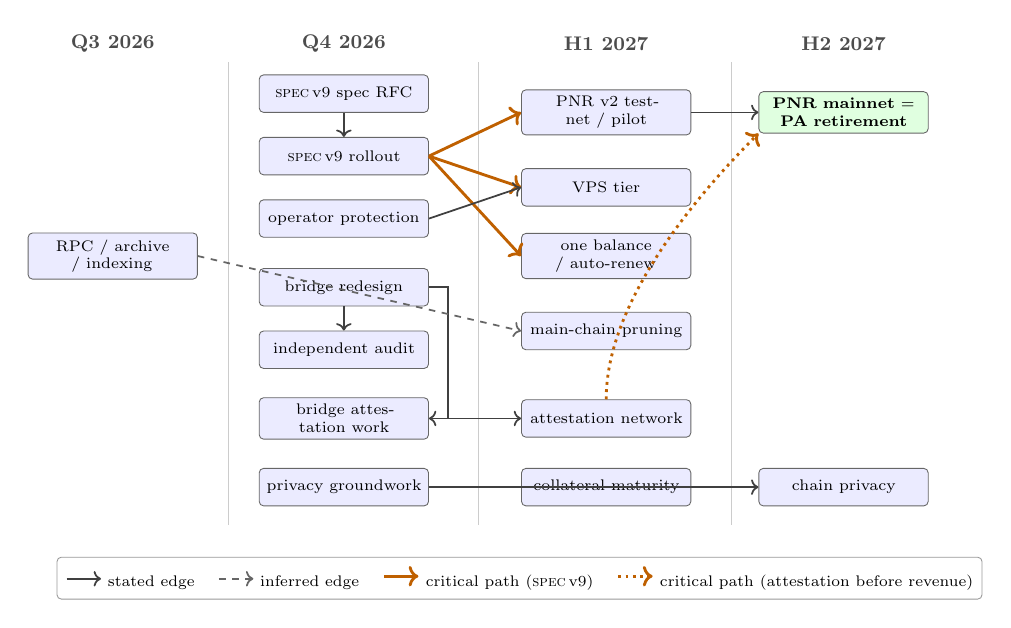
\begin{tikzpicture}[font=\scriptsize,
  n/.style={draw=black!60, rounded corners=2pt, fill=blue!8, align=center, inner sep=3pt,
            text width=2.5cm, minimum height=6mm},
  lane/.style={font=\small\bfseries, text=black!70},
  st/.style={->, thick, black!75},
  inf/.style={->, thick, black!60, dashed},
  cp/.style={->, line width=1.3pt, orange!75!black},
]
\node[lane] at (0,7.0)   {Q3 2026};
\node[lane] at (3.7,7.0) {Q4 2026};
\node[lane] at (7.9,7.0) {H1 2027};
\node[lane] at (11.7,7.0){H2 2027};
\draw[black!20] (1.85,-0.7) -- (1.85,6.7);
\draw[black!20] (5.85,-0.7) -- (5.85,6.7);
\draw[black!20] (9.9,-0.7)  -- (9.9,6.7);

\node[n] (rpc)  at (0,3.6)   {RPC / archive / indexing};
\node[n] (rfc)  at (3.7,6.2) {\specv{9} spec RFC};
\node[n] (v9)   at (3.7,5.2) {\specv{9} rollout};
\node[n] (opro) at (3.7,4.2) {operator protection};
\node[n] (brd)  at (3.7,3.1) {bridge redesign};
\node[n] (aud)  at (3.7,2.1) {independent audit};
\node[n] (att4) at (3.7,1.0) {bridge attestation work};
\node[n] (priv) at (3.7,-0.1){privacy groundwork};

\node[n] (pnr)  at (7.9,5.9) {\PNR{} v2 testnet / pilot};
\node[n] (vps)  at (7.9,4.7) {VPS tier};
\node[n] (bal)  at (7.9,3.6) {one balance / auto-renew};
\node[n] (prun) at (7.9,2.4) {main-chain pruning};
\node[n] (attn) at (7.9,1.0) {attestation network};
\node[n] (coll) at (7.9,-0.1){collateral maturity};

\node[n, fill=green!12] (act) at (11.7,5.9) {\textbf{\PNR{} mainnet $=$ PA retirement}};
\node[n] (chpr) at (11.7,-0.1) {chain privacy};

\draw[st] (rfc) -- (v9);
\draw[cp] (v9.east) -- (pnr.west);
\draw[cp] (v9.east) -- (vps.west);
\draw[cp] (v9.east) -- (bal.west);
\draw[st] (opro.east) -- (vps.west);
\draw[st] (brd) -- (aud);
\draw[st] (brd.east) -- ++(0.3,0) |- (att4.east);
\draw[st] (att4.east) -- (attn.west);
\draw[st] (priv.east) -- (chpr.west);
\draw[st] (pnr.east) -- (act.west);
\draw[inf] (rpc.east) -- (prun.west);
\draw[cp, dotted] (attn.north) .. controls +(0,1.5) and +(-1.1,-1.1) .. (act.south west);

\node[draw=black!40, fill=white, rounded corners=2pt, align=left, inner sep=4pt,
      anchor=south west, font=\scriptsize] at (-0.9,-1.9)
  {\tikz{\draw[st] (0,0)--(0.55,0);} stated edge \quad
   \tikz{\draw[inf] (0,0)--(0.55,0);} inferred edge \quad
   \tikz{\draw[cp] (0,0)--(0.55,0);} critical path (\specv{9}) \quad
   \tikz{\draw[cp,dotted] (0,0)--(0.55,0);} critical path (attestation before revenue)};
\end{tikzpicture}
\caption{Roadmap item dependency graph, clustered by stated quarter.}
\label{fig:e3-depgraph}
\end{figure}

The figure shows the edges of Table~\ref{tab:e3-edges} as a directed graph.


%% =====================================================================
\subsection{Timeline-only items}\label{sec:E4}

\texttt{timeline.html} is a separately hand-authored artifact with its own item set and no prose
counterpart in \texttt{flux-roadmap-public.\allowbreak{}md}; the build pipeline treats the prose document as
the sole source for the rendered PDF and web fragment
\srcdoc{flux-roadmap/public/build-public.sh:7-13}. The 23 items below are reported as a distinct,
lower-weight class of signal — UI tiles, not committed roadmap items — and are never merged into
\S\ref{sec:E1}'s tables.

\begingroup
\footnotesize
\setlength{\tabcolsep}{4pt}
\begin{longtable}{p{0.18\linewidth}p{0.05\linewidth}p{0.13\linewidth}p{0.09\linewidth}p{0.44\linewidth}}
\caption{Items appearing only in \texttt{timeline.html}, reported as weak signals per C12, not commitments.}\label{tab:e4-timeline}\\
\hline
\textbf{Item} & \textbf{Pillar} & \textbf{Maturity} & \textbf{Quarter} & \textbf{Note / citation} \\
\hline
\endfirsthead
\multicolumn{5}{l}{\textit{Table \thetable\ continued}}\\
\hline
\textbf{Item} & \textbf{Pillar} & \textbf{Maturity} & \textbf{Quarter} & \textbf{Note / citation} \\
\hline
\endhead
\hline
\endfoot
\hline
\endlastfoot
bStocks in Zelcore & P8 & IN-PROGRESS & Q3 2026 & \srcroadmap{timeline.html:112-113} \\
Kaspa tokens (``Mass-aware fees $\cdot$ KRC assets'') & P8 & not stated & Q3 2026 & \srcroadmap{timeline.html:115-116} \\
Earn \& staking (``Live APY $\cdot$ Titan'') & P2, P8 & SHIPPED-per-label & Q3 2026 & \srcroadmap{timeline.html:118-119} \\
Fusion transparency (``Per-chain reserves published'') & P8, P2 & not stated & Q3 2026 & \srcroadmap{timeline.html:127-128} \\
SSP Enterprise onboarding (``First marquee clients live'') & P8, P7 & SHIPPED-per-label & Q3 2026 & \srcroadmap{timeline.html:130-131} \\
Flux Foundation (``Ecosystem funding \& governance'') & P7 & not stated & Q3 2026 & \srcroadmap{timeline.html:133-134} \\
FluxAI refocused (``Sellable inference, not chat'') & P6 & not stated & Q3 2026 & \srcroadmap{timeline.html:136-137} \\
Domain Manager overhaul (``Rebuilt $\cdot$ one-click domains'') & P3, P4 & not stated & Q4 2026 & \srcroadmap{timeline.html:175-176} \\
Marketplace push (``Game servers $\cdot$ one-click apps'') & P3 & not stated & Q4 2026 & \srcroadmap{timeline.html:178-179} \\
Inference API (``Paid AI on idle capacity'') & P6 & not stated & Q4 2026 & \srcroadmap{timeline.html:196-197} \\
AI deploy agent (``Chat to deploy $\cdot$ human approval'') & P6 & not stated & Q4 2026 & \srcroadmap{timeline.html:199-200} \\
Zelcore security pack & P8 & not stated & Q4 2026 & Also appears as an H1 2027 sub-item in the prose document. \srcroadmap{timeline.html:202-203} \\
Tax \& CSV export & P8 & not stated & Q4 2026 & Also listed as a sub-item of the Zelcore security pack in \texttt{flux-roadmap-public.\allowbreak{}md}; a separate tile here. \srcroadmap{timeline.html:205-206} \\
SSP Enterprise (``Policy engine $\cdot$ WalletConnect'') & P8, P7 & not stated & Q4 2026 & \srcroadmap{timeline.html:208-209} \\
Transaction screening (``Scam \& drainer warnings'') & P8 & not stated & Q4 2026 & \srcroadmap{timeline.html:211-212} \\
ISO 27001 (``Certification underway'') & P7, P3 & IN-PROGRESS-per-label & Q4 2026 & \srcroadmap{timeline.html:214-215} \\
FluxCore auto-updates (``Self-updating $\cdot$ overclocking controls'') & P1, P9 & not stated & H1 2027 & \srcroadmap{timeline.html:241-242} \\
Torrent application (``Integrated on Flux'') & P3 & not stated & H1 2027 & \srcroadmap{timeline.html:244-245} \\
Fewer, stronger chains (``Long redemption windows'') & P8 & not stated & H1 2027 & Restates the bridge-migration item of Table~\ref{tab:e1-h1} as its own tile. \srcroadmap{timeline.html:247-248} \\
More chains \& assets (``98 chains and growing'') & P8 & SHIPPED-per-label & H1 2027 & The ``98 chains'' figure appears nowhere in \texttt{flux-roadmap-public.\allowbreak{}md}; \notestablished{no corroborating count for parallel-asset chain totals in this paper's corpus}. \srcroadmap{timeline.html:268-269} \\
SSP Key multi-pairing (``One phone, many wallets $\cdot$ CLI'') & P8 & not stated & H1 2027 & Restates the H1 2027 wallets multi-pairing item of Table~\ref{tab:e1-h1} as its own tile. \srcroadmap{timeline.html:274-275} \\
\textbf{New benchmark tool} (``Signed node attestation'') & P1 & not stated & H2 2027 & Bears on \S4 and \S14 together: this paper's benchmark-signature finding is that \texttt{fluxbench}'s result is not bound to the machine that produced it (C13), and this item is the roadmap's own stated fix for exactly that gap (C13). Flagged as the one timeline-only item worth chasing. \srcroadmap{timeline.html:295-296} \\
VPN everywhere (``Windows $\cdot$ Linux'') & P8, P4 & not stated & H2 2027 & Restates the H2 2027 CumulusVPN-platforms item of Table~\ref{tab:e1-h2}, dropping ``Intel macOS.'' \srcroadmap{timeline.html:304-305} \\
\end{longtable}
\endgroup

These items are reported separately, rather than folded into \S\ref{sec:E1}, because the build
pipeline that produces the published PDF and HTML fragment draws only from
\texttt{flux-roadmap-public.\allowbreak{}md}
\srcdoc{flux-roadmap/public/build-public.sh:7-13}: \texttt{timeline.html} is a separately
hand-authored artifact with no equivalent editorial gate, so an item appearing only there carries
materially weaker evidentiary weight than one stated in the prose document.

%% =====================================================================
\subsection{Terminology}\label{sec:E5}

\texttt{notation.tex} is the sole authority for canonical names in this paper; where the roadmap's
own spelling differs from, or is absent relative to, the canonical name, both are given below.

\begingroup
\footnotesize
\begin{longtable}{p{0.22\linewidth}p{0.22\linewidth}p{0.51\linewidth}}
\caption{Roadmap terminology versus this paper's canonical names.}\label{tab:e5-terms}\\
\hline
\textbf{Roadmap's own spelling} & \textbf{Canonical name (\texttt{notation.tex})} & \textbf{Note} \\
\hline
\endfirsthead
\multicolumn{3}{l}{\textit{Table \thetable\ continued}}\\
\hline
\textbf{Roadmap's own spelling} & \textbf{Canonical name (\texttt{notation.tex})} & \textbf{Note} \\
\hline
\endhead
\hline
\endfoot
\hline
\endlastfoot
``FusionX'' (redemption, H1 2027) \srcdoc{flux-roadmap/public/flux-roadmap-public.md:135} and ``Fusion'' (reserve transparency, \texttt{timeline.html}) \srcroadmap{timeline.html:127-128} & \FusionX{} (redemption/exchange product) and \Fusion{} (incumbent custodial bridge) & \texttt{notation.tex} treats these as two distinct canonical names, matching the roadmap's own two distinct usages; the roadmap's bridge-redesign section never names the incumbent bridge it replaces at all, calling it only ``bridge addresses'' \srcdoc{flux-roadmap/public/flux-roadmap-public.md:96-99}. \\
(no tier name used) --- ``operators,'' ``nodes,'' generic ``datacenter tier'' / ``VPS tier'' & \tiers{} = \{\tC{} (\CumulusVPN{} is a product name and is never the Cumulus tier), \tN{}, \tS{}\} & The tier names Cumulus, Nimbus and Stratus appear nowhere in \texttt{public/\allowbreak{}flux-roadmap-public.\allowbreak{}md}, \texttt{public/\allowbreak{}timeline.\allowbreak{}html}, or the PDF text; the canonical names are sourced from \texttt{fluxd}/FluxOS, not from the public roadmap. \\
``FluxCloud'' and ``FluxEdge,'' merged product not separately named \srcdoc{flux-roadmap/public/flux-roadmap-public.md:43} & \FluxCloud{}, \FluxEdge{} & \textbf{Settled: the merged product is \FluxCloud{}} --- ``that's the brand, all available there'' \srcintent{08-answers-round-2.md, round 13}. \FluxEdge{} is retained in this paper only where it names the component as it exists today; the converged product carries the \FluxCloud{} name and no new macro is needed. \\
``PNR v2'' \srcdoc{flux-roadmap/public/flux-roadmap-public.md:111} & \PNR{} (Progressive Node Rewards) & \texttt{notation.tex} flags \PoN{} and \PNR{} as a deliberate terminology hazard: different mechanisms in different layers, trivially confused; both expansions must be given on first use. \\
``FluxOS v9'' / ``v9'' \srcdoc{flux-roadmap/public/flux-roadmap-public.md:52,55} & \specv{9} (the \appspec{} version) & \texttt{notation.tex} reserves ``v9'' exclusively for the application-specification version in this paper; \fluxd{}'s client version 9.1.0 is unrelated and is written out in full, as \daemonversion{}, wherever it appears. \\
``Attestation network'' (opt-in bonded tier, k-of-n verification) \srcdoc{flux-roadmap/public/flux-roadmap-public.md:135} & \SAS{} (System Attestation Service, repo \fluxsas{}) is the \emph{existing} service; the roadmap's bonded network is a distinct, larger, not-yet-built mechanism & The roadmap's item and this paper's \SAS{} share the word ``attestation'' but are not the same mechanism; conflating them is a terminology hazard this paper's evidence flags directly. \\
``VPONs'' / ``Private deployments'' \srcdoc{flux-roadmap/public/flux-roadmap-public.md:83} & \VPON{} (singular macro; private deployment / private overlay network) & The roadmap's plural usage and \texttt{timeline.html}'s ``Private overlay networks'' tile refer to the same singular canonical concept. \\
\end{longtable}
\endgroup

%% Drain this section's float queue before the next begins.
\FloatBarrier


\end{document}
